% -*- Mode:TeX -*-

\documentclass[12pt,twoside]{mitthesis}

%\setcounter{tocdepth}{3}
%\setcounter{secnumdepth}{3}

\usepackage{lgrind}
\usepackage{cmap}
\usepackage[T1]{fontenc}
\pagestyle{plain}

\usepackage[superscript]{cite}

\usepackage{amsmath}
\usepackage{amssymb}
\usepackage{hyperref}

\usepackage{tocloft}

\usepackage{tikz} 
\usepackage{pgfplots}

\usepackage{empheq}
\usepackage[siunitx,cuteinductors,americanvoltages,americancurrents]{circuitikz}
\usepackage{xfrac}

\usepackage{adjustbox}

\usepackage{subcaption}

\usepackage[capitalise]{cleveref}

\usepackage[symbol, flushmargin, hang, perpage]{footmisc}
\renewcommand{\thefootnote}{\fnsymbol{footnote}}

\usepackage[most]{tcolorbox}
\setlength{\parindent}{0pt}
\setlength{\parskip}{6pt}

\newcommand{\listequationsname}{List of Equations}
\newlistof{myequations}{equ}{\listequationsname}
\newcommand{\myequations}[1]{\addcontentsline{equ}{myequations}{\protect\numberline{\theequation} \ \ \, #1}}

\makeatletter
\DeclareRobustCommand{\volume}{\text{\volumedash}V}
\newcommand{\volumedash}{%
  \makebox[0pt][l]{%
    \ooalign{\hfil\hphantom{$\m@th V$}\hfil\cr\kern0.08em--\hfil\cr}%
  }%
}
\makeatother

%% This bit allows you to either specify only the files which you wish to
%% process, or `all' to process all files which you \include.
%% Krishna Sethuraman (1990).

\pgfplotsset{compat=1.3}

\begin{document}

\include{cover}
\pagestyle{plain}
\include{contents}

%\documentclass[11pt]{book}
%
%\setlength{\parindent}{0pt}
%\setlength{\parskip}{8pt}
%
%\usepackage{amsmath}
%\usepackage{amssymb}
%\usepackage{hyperref}
%
%\renewcommand*{\thefootnote}{\fnsymbol{footnote}}
%
%\setcounter{chapter}{0}
%
%\begin{document}
%
%\section*{A Levelized Comparison of \\ Pulsed and Steady-State Tokamaks}
%
%\let\cleardoublepage\relax \tableofcontents \newpage

\chapter{Introducing Fusion Reactor Design}

\begin{figure}
	\centering
\includegraphics[width=0.75\textwidth]{images/fusion_reactor}
	\caption{Cut-Away of Tokamak Reactor} ~\\
	\small The three main components of a magnetic fusion reactor are: the tokamak structure, the plasma fuel, and the spring-like solenoid at the center. Here, the directions of the magnetic field ($B_0$) and plasma current ($I_P$) variables are shown to be in the toroidal direction.
	\label{fig:fusion_reactor}
\end{figure}

\added{The central goal of fusion energy research is to build an economically competitive nuclear reactor. It has long been joked, though, that fusion power will always be twenty years away. This is mainly due to the nonlinearities inherent to a reactor system and the high upfront cost of building new machines. The model developed for this paper uses standard theory and empirical fits to find cost trends from this nonlinear system. An important conclusion is that building an economic reactor using existing technology would be impossible. One solution may be improving magnet technology -- as MIT is exploring with high-temperature superconducting (HTS) tape.}

\added{As can be seen by comparing the European and American/Asian fusion reactor design efforts, though, one of the most important decisions is whether to run the reactor as pulsed (EU\cite{eupulsed,eupulsed_2}) or steady-state (US\cite{ussteady} and Korea\cite{kstar}). The distinction between the two mainly manifests itself in the choice of auxiliary current drive:  inductive  for pulsed and lower hybrid for steady-state.\cite{jeff} With the model built for this thesis, it is possible to perform a direct comparison of these two modes of operations. }

\added{Due to the speed and simplicity of the model, hundreds of reactors can be simulated in minutes. Further, the model has been benchmarked against other ones from the literature\cite{ussteady,arc,process,inputfile}, allowing it to answer several critical questions regarding the comparison of the two modes of operation. A major finding of this is that HTS tape should appear in different places for the two modes of operation: within the central solenoid for pulsed machines and inside the TF coil magnets for steady-state ones. A more basic finding is that pulsed can be competitive and the US should investigate it further. }

\deleted{The central goal of fusion energy research is to build a profitable nuclear reactor. It has long been joked though that fusion power will always be 20-50 years away. This paper lays a framework for exploring reactor space for functional, efficient designs -- based on world experiments during the last half-century. Due to the speed and simplicity of the model, hundreds of reactors can be explored in minutes (outpacing the domestic program slightly).}

\deleted{With this proposed model, interesting reactors can be pinpointed long before engineers hit the blueprints. This should help shorten the time until a profitable reactor, as well as illuminate ways to improve modern plasma theory. Further, it verifies the reasoning of MIT's PSFC to invest in high field, high-temperature superconducting (HTS) tape -- as this technology would lead to much smaller devices.}

\section{Distinguishing Pulsed from Steady-State}

\added{The leading candidate for the first economic, power-producing fusion reactor is a tokamak. As shown in \cref{fig:fusion_reactor}, tokamaks are doughnut-shaped metal structures that use magnets to confine their fusion-grade plasmas. The challenge in building such a device comes from the various physics and engineering constraints it must satisfy -- i.e. not surpassing acceptable levels of neutron damage, plasma pressure, etc.}

\added{One of the most contentious points of reactor design, however, is whether to run it as: pulsed (the European effort\cite{eupulsed,eupulsed_2}) or steady-state (the American/Asian approach\cite{ussteady,kstar}). Here, pulsed operation refers to how a reactor is ramped up and down several times a day. Whereas steady-state implies a machine is functionally kept ramped up the entirety of its fifty-year campaign. These behaviors are shown in \cref{fig:pulses}. The difficulties involves with the two modes of operation are then: cyclical stresses for pulsed and expensive current drive for steady state.\cite{jeff}}

\deleted{When people talk about fusion, they usually talk about plasma physics, and when people talk about plasma physics, they often talk about things like: the sun, lightning, and the aurora borealis. Of these three, the sun is the only nuclear reactor. However, the sun can stay on all day because the massive gravity of its fuel source helps keep it self-contained in space. On Earth, this is not possible -- the plasma fuel needs to be contained by other means (i.e.\ with magnets).}

%\footnote{Plasmas are the fourth state of matter after: solids, liquids, and gases. Fundamentally they are gaseous fluids that respond to electric and magnetic fields.}

\deleted{A tokamak is one of the leading candidates for a profitable fusion reactor. It shares the shape of a doughnut, using magnets to keep a hula hoop of plasma swirling inside it. The difficulty of keeping this plasma swirling though, is that it does not enjoy being spun too fast or squeezed too hard. Conversely, the tokamak housing the plasma does not like taking too much of a beating or being scaled to T-Rex sized proportions. This sets the stage for tokamak reactor design -- building on the various plasma physics and nuclear engineering constraints of the day. }

\deleted{One of the most contentious points of building a tokamak, however, is whether it will be run as: pulsed (the European approach \cite{eupulsed}) or steady-state (the United States effort \cite{ussteady}). Here, pulsed operation refers to how a reactor is turned on and off periodically -- around ten times a day. Whereas, steady state machines are meant to be left on nearly the entirety of their 50-year campaigns. These behaviors are shown in Fig.\ \ref{fig:pulses}.}

\begin{figure}
	\centering
	\begin{adjustbox}{width=0.65\textwidth}
		\large
		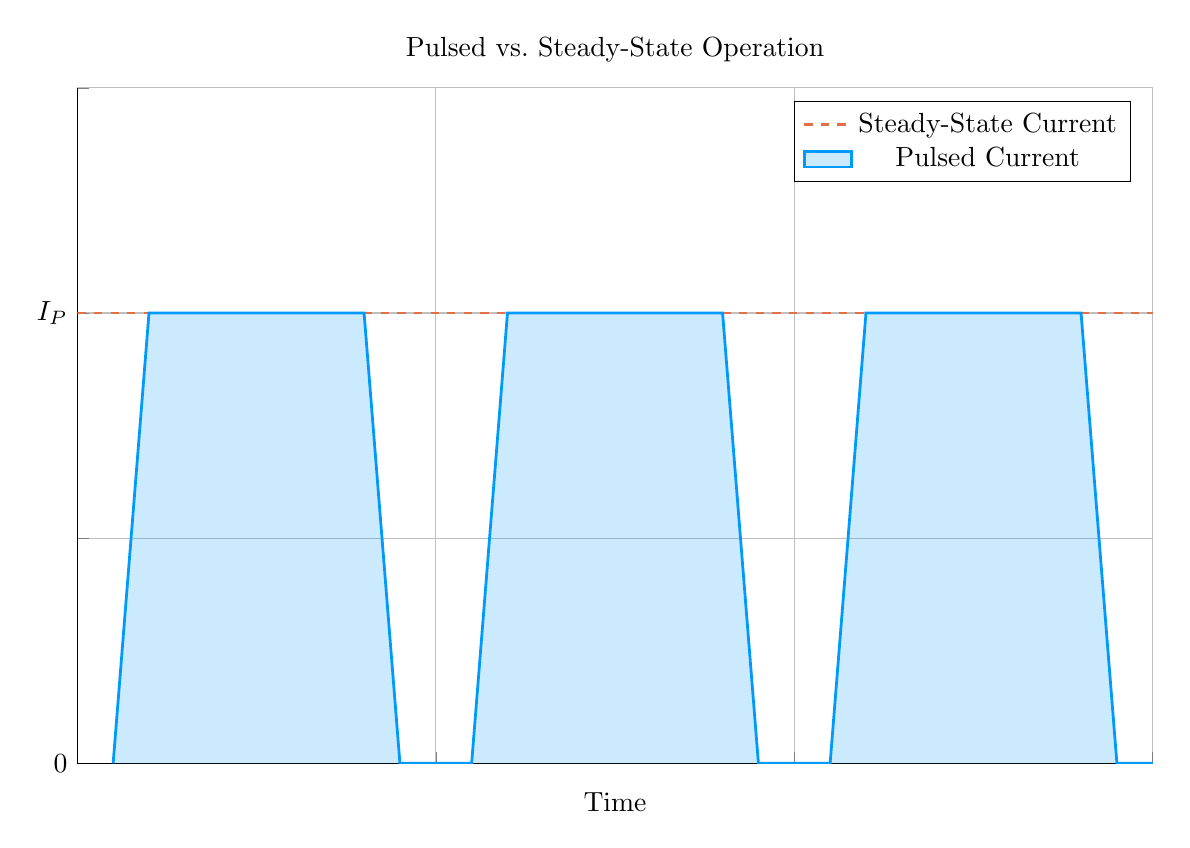
\begin{tikzpicture}[]
\begin{axis}[height = {101.6mm}, ylabel = {}, title = {Pulsed vs.\ Steady-State Operation}, xmin = {0}, xmax = {30}, ymax = {1.5}, xlabel = {Time}, {unbounded coords=jump, scaled x ticks = false, xticklabel style={rotate = 0}, xmajorgrids = true, xtick = {10,20,30}, xticklabels = {}, xtick align = inside, axis lines* = left, scaled y ticks = false, yticklabel style={rotate = 0}, ymajorgrids = true, ytick = {0.0,0.5,1.0,1.5}, yticklabels = {0,,$I_P$,}, ytick align = inside, axis lines* = left,     xshift = 0.0mm,
    yshift = 0.0mm,
    axis background/.style={fill={rgb,1:red,1.00000000;green,1.00000000;blue,1.00000000}}
}, ymin = {0}, width = {152.4mm}]\addplot+ [color = {rgb,1:red,0.88887350;green,0.43564919;blue,0.27812294},
draw opacity=1.0,
line width=1,
dashed,mark = none,
mark size = 2.0,
mark options = {
    color = {rgb,1:red,0.00000000;green,0.00000000;blue,0.00000000}, draw opacity = 1.0,
    fill = {rgb,1:red,0.88887350;green,0.43564919;blue,0.27812294}, fill opacity = 1.0,
    line width = 1,
    rotate = 0,
    solid
}]coordinates {
(0.0, 1.0)
(2.0, 1.0)
(NaN, NaN)
(8.0, 1.0)
(12.0, 1.0)
(NaN, NaN)
(18.0, 1.0)
(22.0, 1.0)
(NaN, NaN)
(28.0, 1.0)
(30.0, 1.0)
};
\addlegendentry{Steady-State Current}
\addplot+ [color = {rgb,1:red,0.00000000;green,0.60560316;blue,0.97868012},
draw opacity=1.0,
line width=1,
solid,mark = none,
mark size = 2.0,
mark options = {
    color = {rgb,1:red,0.00000000;green,0.00000000;blue,0.00000000}, draw opacity = 1.0,
    fill = {rgb,1:red,0.00000000;green,0.60560316;blue,0.97868012}, fill opacity = 1.0,
    line width = 1,
    rotate = 0,
    solid
},fill = {rgb,1:red,0.00000000;green,0.60560316;blue,0.97868012}, fill opacity=0.2,area legend]coordinates {
(1, 0)
(2, 1)
(8, 1)
(9, 0)
(11, 0)
(11, 0)
(12, 1)
(18, 1)
(19, 0)
(21, 0)
(21, 0)
(22, 1)
(28, 1)
(29, 0)
(31, 0)
};
\addlegendentry{Pulsed Current}
\end{axis}

\end{tikzpicture}

	\end{adjustbox}
%	\includegraphics[width=0.85\textwidth]{images/test_image}
	\caption{Comparison of Pulsed and Steady-State Current} ~\\
	\small Inside a pulsed reactor, current is ramped up and down several times a day -- with downtime in-between. Steady state reactors are meant to remain on for weeks or months.
	\label{fig:pulses}
\end{figure}

\replaced{The main way these}{These} two modes of operation, \emph{pulsed} and \emph{steady-state}, \deleted{greatly} influence \replaced{reactor design, though, is}{the design} through the current balance equation (derived later). What this means practically is \replaced{a tokamak plasma requires some current to stay in equilibrium}{tokamaks need current to spin their plasma hoops at some required speed} and this current has to \replaced{be partially generated by auxiliary systems: inductively for pulsed and non-inductively for steady-state.}{come from somewhere. Luckily, the plasma naturally enjoys spinning and provides some assistance through the bootstrap current. The remaining current must then be produced by external means.} \added{To fairly compare the two modes of operation thus requires a generalized handling of current balance that can incorporate both auxiliary systems. }

\deleted{The source of external current drive is what distinguishes pulsed from steady-state devices. Steady-state devices provide the required current assistance either through lasers or particle beams -- this paper's model focusing on a type of laser assistance called lower-hybrid current drive (LHCD). \cite{jeff} Pulsed machines, on the other hand, rely on inductive sources -- which by definition require cycles of charging and discharging several times a day.}

%\footnote{ These inductive sources are akin to a battery on a laptop that must be recharged every so often. }

\deleted{The goal of this document is to show that pulsed and steady-state operation are actually two sides of the same coin. This yields the simple conclusion that a single comprehensive model can run both modes at the flip of a switch. It even opens the opportunity of a hybrid reactor that exists somewhere in between the two.}

%\section{Treating Fusion as a Business}
%
%Plasmas may be interesting, but that is not why countries build billion dollar research experiments. The ultimate goal of fusion research is to develop an energy resource that competes with coal and other base-load power sources (e.g.\ from hydroelectric and nuclear fission power plants). The problem is plasmas are chaotic and hard to contain, while tokamaks are expensive and slow to build. This perfect match has long put the field's projected timeline to that of \emph{fusion never}. \cite{fusionfunding}
%
%\begin{figure}[h]
%	\centering
%	\begin{adjustbox}{width=0.75\textwidth}
%		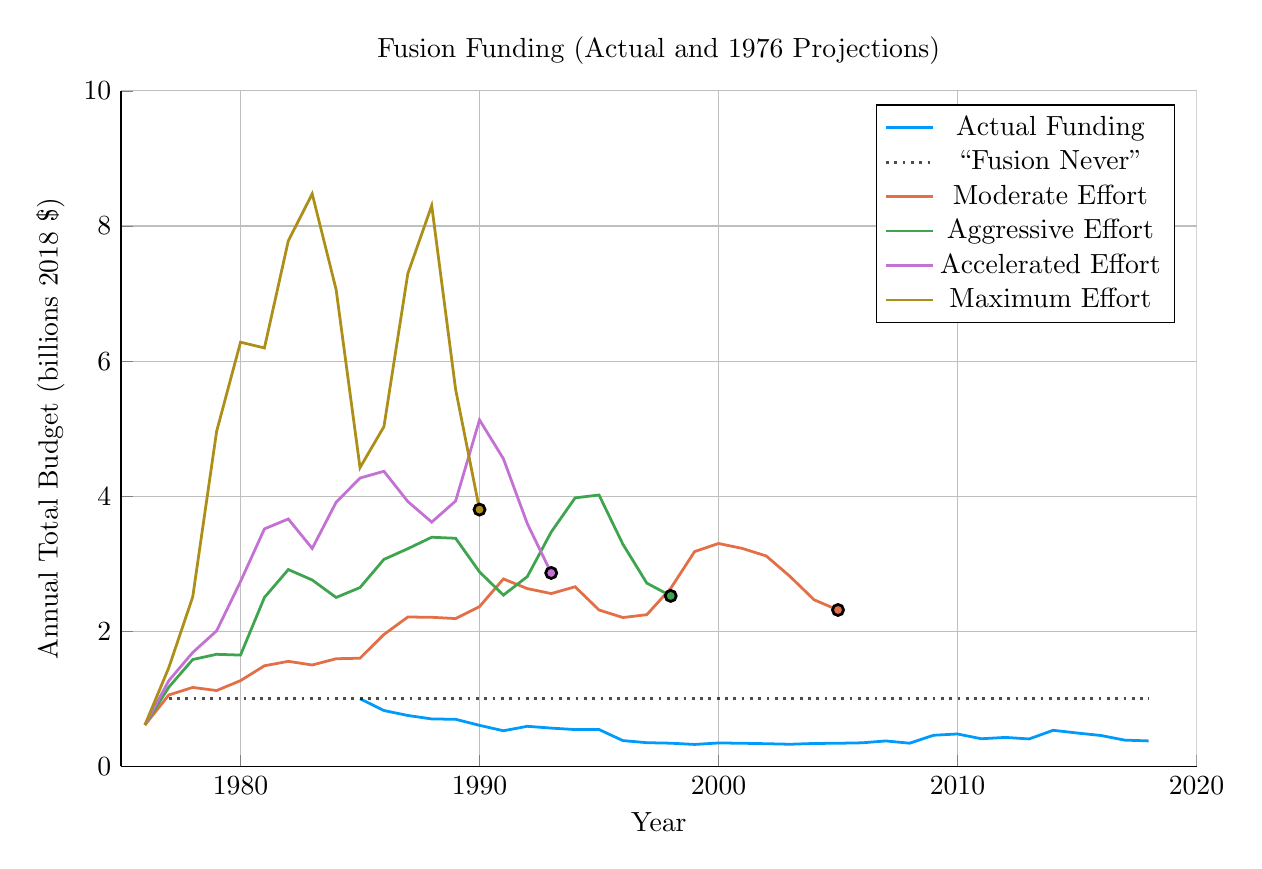
\begin{tikzpicture}[]
\begin{axis}[height = {101.6mm}, ylabel = {Annual Total Budget (billions 2018 \$)}, title = {Fusion Funding (Actual and 1976 Projections)}, xmin = {1975}, xmax = {2020}, ymax = {10}, xlabel = {Year}, {unbounded coords=jump, scaled x ticks = false, xticklabel style={rotate = 0}, xmajorgrids = true, xtick = {1980.0,1990.0,2000.0,2010.0,2020.0}, xticklabels = {1980,1990,2000,2010,2020}, xtick align = inside, axis lines* = left, scaled y ticks = false, yticklabel style={rotate = 0}, ymajorgrids = true, ytick = {0.0,2.0,4.0,6.0,8.0,10.0}, yticklabels = {0,2,4,6,8,10}, ytick align = inside, axis lines* = left,     xshift = 0.0mm,
    yshift = 0.0mm,
    axis background/.style={fill={rgb,1:red,1.00000000;green,1.00000000;blue,1.00000000}}
}, ymin = {0}, width = {152.4mm}]\addplot+ [color = {rgb,1:red,0.00000000;green,0.60560316;blue,0.97868012},
draw opacity=1.0,
line width=1,
solid,mark = none,
mark size = 2.0,
mark options = {
    color = {rgb,1:red,0.00000000;green,0.00000000;blue,0.00000000}, draw opacity = 1.0,
    fill = {rgb,1:red,0.00000000;green,0.60560316;blue,0.97868012}, fill opacity = 1.0,
    line width = 1,
    rotate = 0,
    solid
}]coordinates {
(1985.0, 1.001836)
(1986.0, 0.827367)
(1987.0, 0.754179)
(1988.0, 0.702929)
(1989.0, 0.697497)
(1990.0, 0.608102)
(1991.0, 0.527899)
(1992.0, 0.593976)
(1993.0, 0.567297)
(1994.0, 0.545463)
(1995.0, 0.545963)
(1996.0, 0.382175)
(1997.0, 0.351267)
(1998.0, 0.343818)
(1999.0, 0.325482)
(2000.0, 0.347117)
(2001.0, 0.342814)
(2002.0, 0.336267)
(2003.0, 0.32825)
(2004.0, 0.339832)
(2005.0, 0.342925)
(2006.0, 0.349302)
(2007.0, 0.377075)
(2008.0, 0.343662)
(2009.0, 0.461341)
(2010.0, 0.48051)
(2011.0, 0.409602)
(2012.0, 0.42938)
(2013.0, 0.406833)
(2014.0, 0.534818)
(2015.0, 0.494834)
(2016.0, 0.457833)
(2017.0, 0.389125)
(2018.0, 0.377419)
};
\addlegendentry{Actual Funding}
\addplot+ [color = {rgb,1:red,0.00000000;green,0.00000000;blue,0.00000000},
draw opacity=0.7,
line width=1,
dotted,mark = none,
mark size = 2.0,
mark options = {
    color = {rgb,1:red,0.00000000;green,0.00000000;blue,0.00000000}, draw opacity = 0.7,
    fill = {rgb,1:red,0.00000000;green,0.00000000;blue,0.00000000}, fill opacity = 0.7,
    line width = 1,
    rotate = 0,
    solid
}]coordinates {
(1977, 1)
(2018, 1)
};
\addlegendentry{``Fusion Never''}
\addplot+ [color = {rgb,1:red,0.88887350;green,0.43564919;blue,0.27812294},
draw opacity=1.0,
line width=1,
solid,mark = none,
mark size = 2.0,
mark options = {
    color = {rgb,1:red,0.00000000;green,0.00000000;blue,0.00000000}, draw opacity = 1.0,
    fill = {rgb,1:red,0.88887350;green,0.43564919;blue,0.27812294}, fill opacity = 1.0,
    line width = 1,
    rotate = 0,
    solid
}]coordinates {
(1976.0, 0.61374)
(1977.0, 1.05764)
(1978.0, 1.1695799999999998)
(1979.0, 1.12326)
(1980.0, 1.2699399999999998)
(1981.0, 1.48996)
(1982.0, 1.55558)
(1983.0, 1.5015399999999999)
(1984.0, 1.59418)
(1985.0, 1.6018999999999999)
(1986.0, 1.9531599999999998)
(1987.0, 2.2117799999999996)
(1988.0, 2.2079199999999997)
(1989.0, 2.18862)
(1990.0, 2.36618)
(1991.0, 2.77534)
(1992.0, 2.63252)
(1993.0, 2.55918)
(1994.0, 2.65954)
(1995.0, 2.316)
(1996.0, 2.2040599999999997)
(1997.0, 2.24652)
(1998.0, 2.63638)
(1999.0, 3.18064)
(2000.0, 3.3002999999999996)
(2001.0, 3.2269599999999996)
(2002.0, 3.11502)
(2003.0, 2.8100799999999997)
(2004.0, 2.4665399999999997)
(2005.0, 2.316)
};
\addlegendentry{Moderate Effort}
\addplot+[draw=none, color = {rgb,1:red,0.88887350;green,0.43564919;blue,0.27812294},
draw opacity=1.0,
line width=0,
solid,mark = *,
mark size = 2.0,
mark options = {
    color = {rgb,1:red,0.00000000;green,0.00000000;blue,0.00000000}, draw opacity = 1.0,
    fill = {rgb,1:red,0.88887350;green,0.43564919;blue,0.27812294}, fill opacity = 1.0,
    line width = 1,
    rotate = 0,
    solid
},forget plot] coordinates {
(2005.0, 2.316)
};
\addplot+ [color = {rgb,1:red,0.24222430;green,0.64327509;blue,0.30444865},
draw opacity=1.0,
line width=1,
solid,mark = none,
mark size = 2.0,
mark options = {
    color = {rgb,1:red,0.00000000;green,0.00000000;blue,0.00000000}, draw opacity = 1.0,
    fill = {rgb,1:red,0.24222430;green,0.64327509;blue,0.30444865}, fill opacity = 1.0,
    line width = 1,
    rotate = 0,
    solid
}]coordinates {
(1976.0, 0.61374)
(1977.0, 1.1734399999999998)
(1978.0, 1.5825999999999998)
(1979.0, 1.6598)
(1980.0, 1.6482199999999998)
(1981.0, 2.50128)
(1982.0, 2.9143)
(1983.0, 2.7598999999999996)
(1984.0, 2.50128)
(1985.0, 2.64796)
(1986.0, 3.06484)
(1987.0, 3.2230999999999996)
(1988.0, 3.39294)
(1989.0, 3.3775)
(1990.0, 2.8795599999999997)
(1991.0, 2.5360199999999997)
(1992.0, 2.8100799999999997)
(1993.0, 3.47014)
(1994.0, 3.9757999999999996)
(1995.0, 4.01826)
(1996.0, 3.2887199999999996)
(1997.0, 2.71358)
(1998.0, 2.52444)
};
\addlegendentry{Aggressive Effort}
\addplot+[draw=none, color = {rgb,1:red,0.24222430;green,0.64327509;blue,0.30444865},
draw opacity=1.0,
line width=0,
solid,mark = *,
mark size = 2.0,
mark options = {
    color = {rgb,1:red,0.00000000;green,0.00000000;blue,0.00000000}, draw opacity = 1.0,
    fill = {rgb,1:red,0.24222430;green,0.64327509;blue,0.30444865}, fill opacity = 1.0,
    line width = 1,
    rotate = 0,
    solid
},forget plot] coordinates {
(1998.0, 2.52444)
};
\addplot+ [color = {rgb,1:red,0.76444018;green,0.44411178;blue,0.82429754},
draw opacity=1.0,
line width=1,
solid,mark = none,
mark size = 2.0,
mark options = {
    color = {rgb,1:red,0.00000000;green,0.00000000;blue,0.00000000}, draw opacity = 1.0,
    fill = {rgb,1:red,0.76444018;green,0.44411178;blue,0.82429754}, fill opacity = 1.0,
    line width = 1,
    rotate = 0,
    solid
}]coordinates {
(1976.0, 0.61374)
(1977.0, 1.2699399999999998)
(1978.0, 1.68682)
(1979.0, 2.0071999999999997)
(1980.0, 2.7367399999999997)
(1981.0, 3.51646)
(1982.0, 3.66314)
(1983.0, 3.2269599999999996)
(1984.0, 3.9101799999999995)
(1985.0, 4.269159999999999)
(1986.0, 4.36952)
(1987.0, 3.92176)
(1988.0, 3.6168199999999997)
(1989.0, 3.92948)
(1990.0, 5.1299399999999995)
(1991.0, 4.554799999999999)
(1992.0, 3.59366)
(1993.0, 2.8641199999999998)
};
\addlegendentry{Accelerated Effort}
\addplot+[draw=none, color = {rgb,1:red,0.76444018;green,0.44411178;blue,0.82429754},
draw opacity=1.0,
line width=0,
solid,mark = *,
mark size = 2.0,
mark options = {
    color = {rgb,1:red,0.00000000;green,0.00000000;blue,0.00000000}, draw opacity = 1.0,
    fill = {rgb,1:red,0.76444018;green,0.44411178;blue,0.82429754}, fill opacity = 1.0,
    line width = 1,
    rotate = 0,
    solid
},forget plot] coordinates {
(1993.0, 2.8641199999999998)
};
\addplot+ [color = {rgb,1:red,0.67554396;green,0.55566233;blue,0.09423434},
draw opacity=1.0,
line width=1,
solid,mark = none,
mark size = 2.0,
mark options = {
    color = {rgb,1:red,0.00000000;green,0.00000000;blue,0.00000000}, draw opacity = 1.0,
    fill = {rgb,1:red,0.67554396;green,0.55566233;blue,0.09423434}, fill opacity = 1.0,
    line width = 1,
    rotate = 0,
    solid
}]coordinates {
(1976.0, 0.61374)
(1977.0, 1.46294)
(1978.0, 2.509)
(1979.0, 4.9601)
(1980.0, 6.28022)
(1981.0, 6.1953)
(1982.0, 7.781759999999999)
(1983.0, 8.47656)
(1984.0, 7.059939999999999)
(1985.0, 4.423559999999999)
(1986.0, 5.029579999999999)
(1987.0, 7.2954)
(1988.0, 8.302859999999999)
(1989.0, 5.58156)
(1990.0, 3.8021)
};
\addlegendentry{Maximum Effort}
\addplot+[draw=none, color = {rgb,1:red,0.67554396;green,0.55566233;blue,0.09423434},
draw opacity=1.0,
line width=0,
solid,mark = *,
mark size = 2.0,
mark options = {
    color = {rgb,1:red,0.00000000;green,0.00000000;blue,0.00000000}, draw opacity = 1.0,
    fill = {rgb,1:red,0.67554396;green,0.55566233;blue,0.09423434}, fill opacity = 1.0,
    line width = 1,
    rotate = 0,
    solid
},forget plot] coordinates {
(1990.0, 3.8021)
};
\end{axis}

\end{tikzpicture}

%	\end{adjustbox}
%%	\includegraphics[width=0.75\textwidth]{images/test_image}
%	\caption{Fusion Never Funding Timeline} ~\\
%	\small Comparison of Projected Timelines of Fusion from 1976 with Actual DOE Budgets. \cite{doe87, doe19} \\ The dotted line is popularly referred to in the community as ``Fusion Never.'' \cite{fusionnever}
%\end{figure}
%
%The major problem with containing a plasma in a reactor is that a plasma does not want to be contained. Since the early days of fusion research, plasmas have often found escape mechanisms. When presented with a magnetic bottle, they found their way out the top. In a tokamak, they attack the outer edges like an overinflated tire-tube. Fusion energy has seemed to remain a Tantalizing effort -- within arms reach, but staunchly guarded by a shroud of instabilities.
%
%The truth is plasmas are extremely chaotic: they show nonlinear behavior in almost everything they do. As of now, no theory or supercomputer-backed code can predict even something so fundamental to design as the movement of energy and particles within a tokamak. As such, the field has adopted several rules of thumb and empirical scalings -- based on the last half century of experiments -- which help one navigate around a plasma's finicky behavior.
%
%The two most widely used rules of thumb within the fusion design community are: the Greenwald density limit and the ELMy H-Mode confinement time scaling law. As such, the model in this document heavily utilizes the two to make a quick running code. These two relations are also why this model -- which happens to be zero-dimensional -- can reproduce with high fidelity the answers from three-dimensional codes, which can take days, weeks, or even months to run!
%
%\begin{figure}
%	\centering
%	\begin{adjustbox}{width=0.75\textwidth}
%		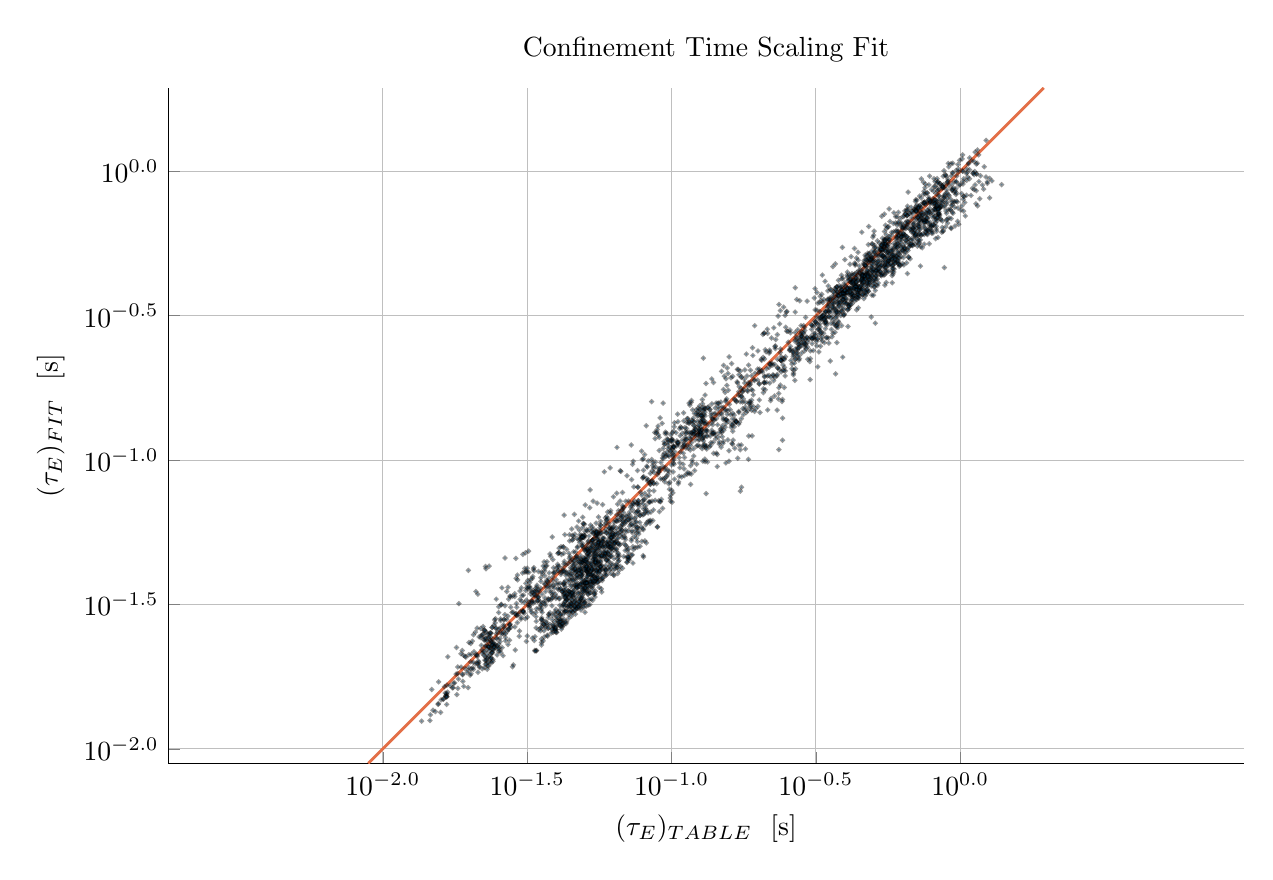
\begin{tikzpicture}[]
\begin{axis}[height = {101.6mm}, axis equal = {true}, ylabel = {$(\tau_E)_{ FIT } \ \ [ \textnormal{s} ]$}, title = {Confinement Time Scaling Fit}, xmin = {0.008904842990761705}, xmax = {1.9473999999999996}, ymax = {1.9473999999999996}, ymode = {log}, xlabel = {$(\tau_E)_{ TABLE } \ \ [ \textnormal{s} ]$}, {unbounded coords=jump, scaled x ticks = false, xticklabel style={rotate = 0}, log basis x=10, xmajorgrids = true, xtick = {0.01,0.03162277660168379,0.1,0.31622776601683794,1.0}, xticklabels = {$10^{-2.0}$,$10^{-1.5}$,$10^{-1.0}$,$10^{-0.5}$,$10^{0.0}$}, xtick align = inside, axis lines* = left, scaled y ticks = false, yticklabel style={rotate = 0}, log basis y=10, ymajorgrids = true, ytick = {0.01,0.03162277660168379,0.1,0.31622776601683794,1.0}, yticklabels = {$10^{-2.0}$,$10^{-1.5}$,$10^{-1.0}$,$10^{-0.5}$,$10^{0.0}$}, ytick align = inside, axis lines* = left,     xshift = 0.0mm,
    yshift = 0.0mm,
    axis background/.style={fill={rgb,1:red,1.00000000;green,1.00000000;blue,1.00000000}}
}, xmode = {log}, ymin = {0.008904842990761705}, width = {152.4mm}]\addplot+[draw=none, color = {rgb,1:red,0.00000000;green,0.60560316;blue,0.97868012},
draw opacity=0.4,
line width=0,
solid,mark = *,
mark size = 0.325,
mark options = {
    color = {rgb,1:red,0.00000000;green,0.00000000;blue,0.00000000}, draw opacity = 0.4,
    fill = {rgb,1:red,0.00000000;green,0.60560316;blue,0.97868012}, fill opacity = 0.4,
    line width = 1,
    rotate = 0,
    solid
},forget plot] coordinates {
(0.048709999999999996, 0.03286927009465151)
(0.047479999999999994, 0.030718782340371346)
(0.056709999999999997, 0.04427687673230967)
(0.06154, 0.040523205193333994)
(0.049249999999999995, 0.031000215657666388)
(0.046439999999999995, 0.03902384637413358)
(0.04536, 0.03366158264691253)
(0.041229999999999996, 0.029311430641277475)
(0.04224, 0.03489492877112558)
(0.05357, 0.03985677848149215)
(0.042449999999999995, 0.030139467297048302)
(0.04393, 0.03525642598465171)
(0.037579999999999995, 0.029115058174186102)
(0.040589999999999994, 0.03552938448965956)
(0.016339999999999997, 0.016414220556232706)
(0.01926, 0.018966660638066977)
(0.014769999999999998, 0.01604916788911629)
(0.020909999999999998, 0.019687625330862386)
(0.014559999999999998, 0.01252323235667468)
(0.016659999999999998, 0.016615842361327)
(0.017099999999999997, 0.016562775820865377)
(0.025429999999999998, 0.024119656293897448)
(0.01834, 0.03183654298531315)
(0.02225, 0.026522518089311862)
(0.02354, 0.023762954142859543)
(0.01883, 0.02190554572449257)
(0.0156, 0.0170549295762654)
(0.01678, 0.020822704009415233)
(0.154, 0.14943255990407037)
(0.17639999999999997, 0.1506224447310805)
(0.7525999999999999, 0.7841653529419872)
(0.7196999999999999, 0.7123510444198007)
(0.7581, 0.7126653992395249)
(0.5971, 0.6636747785042374)
(0.5545, 0.6034081737695671)
(0.5620999999999999, 0.5855426425362842)
(0.7231, 0.611757051674103)
(0.7314999999999999, 0.6000776436052295)
(0.8261999999999999, 0.7332080576221435)
(0.8526999999999999, 0.6874473851854792)
(0.7659999999999999, 0.6249854199535853)
(0.8212999999999999, 0.6647675128338589)
(0.7968, 0.6202645990011652)
(1.1369999999999998, 0.8572954951071405)
(0.8379, 0.709498458538988)
(0.7112999999999999, 0.6481476339591892)
(0.8383999999999999, 0.7100253242029977)
(0.9772, 0.7850517774047457)
(0.6932999999999999, 0.6449986085844157)
(0.7078, 0.5696128161569505)
(0.7666999999999999, 0.6076651618162499)
(0.7231, 0.8218656209469912)
(0.7654, 0.7824204839027497)
(0.8880999999999999, 0.9751544259782554)
(0.9436, 0.987045215482296)
(0.982, 1.0567556111003251)
(1.0659999999999998, 1.0600221351309262)
(1.021, 1.0023421135083617)
(1.037, 0.780421246365204)
(1.0139999999999998, 0.7598649860996711)
(0.9391999999999999, 0.722374477345195)
(0.7876, 0.7737488110528499)
(0.7564, 0.8355652777917266)
(0.8073999999999999, 0.7829615268340135)
(0.6101, 0.662119064106307)
(0.5015, 0.6015695673902948)
(0.7323999999999999, 0.8090796506003152)
(0.6535, 0.7394639493973881)
(0.5972, 0.6975536633839833)
(0.8778999999999999, 0.7874999827504517)
(0.7773, 0.8125562886500788)
(0.6810999999999999, 0.7238692523345119)
(0.6392, 0.701072652615907)
(0.6046999999999999, 0.6507248504722397)
(0.9085, 1.0662323587837632)
(0.746, 0.9171741777262944)
(0.6601999999999999, 0.8477587902173862)
(1.019, 1.1402820961295275)
(0.9123, 1.0371038527895822)
(0.5081, 0.5255375119481419)
(0.7402, 0.6843189302449205)
(0.7313999999999999, 0.6912025500896107)
(1.0779999999999998, 1.1138270195034614)
(0.6314, 0.6309700937894861)
(0.9303999999999999, 0.9647835607071941)
(0.8503, 0.9084098651600415)
(0.8125, 0.8871934724039697)
(0.9943, 1.0920838325900788)
(0.8109999999999999, 0.94316240550339)
(0.7583, 0.9027068941508603)
(0.8357, 0.9197400869136341)
(0.6762999999999999, 0.7509390530838264)
(0.6529999999999999, 0.7031904860947172)
(0.3892, 0.34318485870648646)
(0.34049999999999997, 0.3124029593731834)
(0.45299999999999996, 0.3908324185235881)
(0.44149999999999995, 0.37445805641759866)
(0.5680999999999999, 0.519309036063986)
(0.5427, 0.470258508275619)
(0.3973, 0.3208880474419727)
(0.4023, 0.3620545624474692)
(0.36279999999999996, 0.3723269788644909)
(0.5475, 0.4394327211967968)
(0.3898, 0.37922457801357046)
(0.31279999999999997, 0.303118325347936)
(0.38389999999999996, 0.35281373501460195)
(0.3181, 0.31386085182034285)
(0.7142, 0.6930925801653104)
(0.6252, 0.6626568011479417)
(0.6154999999999999, 0.5263153459242683)
(0.9141999999999999, 0.6902582143865932)
(0.7587999999999999, 0.6215886466745869)
(0.6337999999999999, 0.5997015869390643)
(0.9221999999999999, 0.7382203149764545)
(0.6928, 0.6177290812059213)
(0.7125999999999999, 0.6963967594591091)
(0.21899999999999997, 0.18496435234301067)
(0.20789999999999997, 0.1766203805469118)
(0.26499999999999996, 0.20490261922028621)
(0.4225, 0.34891440428748743)
(0.4118, 0.3421446077261888)
(0.2397, 0.22159945467095882)
(0.26959999999999995, 0.22409261472703068)
(0.3127, 0.2631427459860977)
(0.32389999999999997, 0.2832737570128158)
(0.8515999999999999, 0.9068928303444452)
(0.8177, 0.9220516908419841)
(1.0179999999999998, 1.002889177259622)
(0.5892999999999999, 0.7186483132855688)
(0.9675999999999999, 0.918899482262656)
(0.8809999999999999, 0.4645188486258639)
(1.077, 1.013495270683344)
(0.5667, 0.7415870515780109)
(0.5344, 0.6992580529977903)
(0.5457, 0.7114200487063042)
(0.6599999999999999, 0.568829584256022)
(0.7506999999999999, 0.604323636235005)
(0.7131, 0.5987909231331726)
(0.6576, 0.5815966808550769)
(0.6386, 0.6040200009888924)
(0.4816, 0.6444934910993216)
(0.45589999999999997, 0.6160051006574458)
(0.6427999999999999, 0.7305600248168257)
(0.8285999999999999, 0.7476043736628556)
(0.6534, 0.6544069370264392)
(0.6638999999999999, 0.6723198321350972)
(0.5883999999999999, 0.5629685596654105)
(0.6073999999999999, 0.5947667114406178)
(0.5639, 0.5731530731910407)
(0.6101, 0.6034835968431853)
(0.6638999999999999, 0.5863468310710566)
(0.6346999999999999, 0.5309682418246683)
(0.5062, 0.456996379113654)
(0.6548999999999999, 0.703107054401337)
(0.5526, 0.5545528151553201)
(0.8658999999999999, 0.7858011508612296)
(0.7361, 0.7026740161837454)
(0.734, 0.7080907193345652)
(0.722, 0.7026124938878728)
(0.9287, 1.0629014859458583)
(0.7698999999999999, 0.84074579772222)
(0.8176, 0.8870105921186713)
(0.5843999999999999, 0.5035404234450113)
(0.9373999999999999, 0.8698220688660848)
(0.9337, 0.8623382177770421)
(0.8964, 0.7160170198322513)
(0.7332, 0.9423078640879671)
(0.7831999999999999, 0.963224279565402)
(0.9906999999999999, 0.8952623033567918)
(0.9087, 0.8308130537672082)
(0.7955, 0.8658102097350978)
(0.9360999999999999, 0.9039593399896794)
(0.7863, 0.714131359979918)
(0.8229, 0.740299033130453)
(0.823, 0.760314511413916)
(0.7636999999999999, 0.7163144408463683)
(0.6311, 0.5556779797096207)
(0.6262, 0.6533313908678976)
(0.8946999999999999, 0.9586908006605939)
(0.8576999999999999, 0.7537146014939096)
(0.8473999999999999, 0.7461424250229518)
(0.9255, 0.801575405231461)
(0.8498, 0.7649223531344689)
(0.7823, 0.7268518889656576)
(0.8255999999999999, 0.7470872412684922)
(0.8631, 0.7753860665056598)
(0.7994, 0.728145541191726)
(0.8747999999999999, 0.8208827079316118)
(1.015, 1.1045865073889138)
(1.1609999999999998, 0.9219761380746218)
(0.7623, 0.6715119057586799)
(0.7824, 0.6467686006890678)
(0.5243, 0.564617572937227)
(0.5503999999999999, 0.5783318044105018)
(0.5407, 0.5701439812605221)
(0.5317999999999999, 0.5494542896098417)
(0.5491999999999999, 0.5670933149802504)
(0.5455, 0.5598085924937554)
(0.8478, 0.7018507562099994)
(0.7223999999999999, 0.6570441876740942)
(0.8067, 0.7135500971429034)
(0.7686999999999999, 0.6885128255514706)
(0.7448999999999999, 0.6760240646258281)
(0.7343, 0.6742929760912958)
(0.6597999999999999, 0.7354882011318915)
(0.6793999999999999, 0.7289884081681665)
(0.6546, 0.7051597393592424)
(0.9087999999999999, 0.7368656746766299)
(0.7526999999999999, 0.671806203783079)
(0.7545, 0.8781283223894364)
(0.969, 1.0091726548574242)
(0.9864999999999999, 0.9978820947672817)
(0.9519, 0.8476711232851686)
(0.8273999999999999, 0.778663500363082)
(0.8248, 0.7801934517664398)
(0.6835, 0.6627837535553688)
(0.6928, 0.6114247462326845)
(0.7931999999999999, 0.6269714335560767)
(0.7208, 0.6045147201505461)
(0.6963999999999999, 0.6028585041743847)
(0.8253999999999999, 0.6317543998575686)
(0.6675, 0.5602136085491106)
(0.7319, 0.6026263780884397)
(0.6533, 0.5360321914526158)
(0.564, 0.4904554472531542)
(0.9439, 0.7157171194446946)
(0.7939999999999999, 0.6411620402371146)
(0.8091999999999999, 0.6525781912908896)
(0.7292, 0.5485933677696657)
(0.6357999999999999, 0.503286345980577)
(0.6447999999999999, 0.5185162967617107)
(1.069, 1.0695180372896376)
(0.8583, 0.8908809768320126)
(0.8087, 0.8543034142940075)
(0.8318, 0.9446369769051516)
(0.7786, 0.8979525071302351)
(1.1219999999999999, 0.9996281574893591)
(1.107, 0.9853860242113884)
(1.2109999999999999, 1.0380777356700828)
(1.109, 0.988185626984255)
(0.8967999999999999, 0.7722301840545289)
(0.824, 0.8390911317907782)
(0.8246, 0.7494173273698013)
(0.7246999999999999, 0.6803976433290927)
(0.6926, 0.6607682224597816)
(0.8103999999999999, 0.7710346210832281)
(0.7748999999999999, 0.7325112272388337)
(0.7414999999999999, 0.7062682017319861)
(0.8249, 0.6842066249663288)
(0.8475999999999999, 0.7093971409693103)
(0.7781999999999999, 0.6302194723063099)
(0.7003999999999999, 0.6008831528899192)
(0.6518999999999999, 0.5945976708252837)
(0.7195999999999999, 0.5780911978357602)
(0.7698999999999999, 0.6045774400058568)
(0.6951999999999999, 0.5594902956731888)
(0.6265999999999999, 0.5281946682083224)
(1.0519999999999998, 0.9316449640552941)
(1.011, 0.8373271253227542)
(1.0619999999999998, 0.9564802790915702)
(0.9991, 0.8998058834673238)
(1.1019999999999999, 0.874362127898913)
(0.9502999999999999, 0.7861813492490419)
(1.1929999999999998, 0.8970574608241824)
(1.1409999999999998, 0.9798783118539908)
(1.1389999999999998, 0.981247441890904)
(0.7454, 0.6506062999832742)
(0.7213999999999999, 0.6316980480914915)
(0.7511, 0.6382470829505086)
(1.168, 0.8045488413734408)
(1.1329999999999998, 0.7723998453123871)
(1.2049999999999998, 0.8686731269524)
(0.8418, 0.7105640304650586)
(0.8438, 0.7167529167481481)
(0.8319, 0.6761440014142099)
(0.7971999999999999, 0.647212185326572)
(0.8099999999999999, 0.6507837939912798)
(0.954, 0.7838744415871535)
(1.0279999999999998, 0.8191939822720388)
(1.029, 0.8188141254422304)
(0.9371999999999999, 0.765214397024378)
(1.0219999999999998, 0.9050020965486358)
(1.1449999999999998, 1.0674931488210169)
(1.136, 1.0609598989430766)
(0.9721, 0.9642173576087313)
(0.8966, 0.8641697646781274)
(0.8880999999999999, 0.8373748291165626)
(0.8997999999999999, 0.8442042621804475)
(1.0219999999999998, 0.9220333467704045)
(1.126, 0.897657994702853)
(1.2879999999999998, 0.9272527550966493)
(0.8389, 0.7182547844853155)
(0.9348, 0.7828004050235056)
(1.051, 0.8269739428545848)
(1.0239999999999998, 0.8005745674982954)
(1.158, 1.1412196875478482)
(0.8996, 0.8065770952173787)
(0.9666999999999999, 0.8315473131899693)
(0.8414999999999999, 0.7684067296642498)
(0.8493999999999999, 0.7527319188772996)
(0.8481, 0.7458196646149527)
(0.8429, 0.7423208728716764)
(0.8990999999999999, 0.7842614607464142)
(0.8253999999999999, 0.7485587864344085)
(0.8107, 0.7384132406448961)
(0.8147, 0.7410312659641048)
(0.9854999999999999, 1.0196276084818066)
(1.1469999999999998, 1.1863286392932)
(1.126, 1.1666665208852889)
(0.9404999999999999, 0.8611051902461748)
(0.7303, 0.7213915082892701)
(1.0959999999999999, 1.0877850615898468)
(1.117, 1.0833298051794935)
(1.057, 0.9923729605851154)
(0.9539, 0.9233369235535771)
(1.2289999999999999, 1.2805920757347342)
(0.8688999999999999, 0.8918437252115444)
(0.8352999999999999, 0.8716065387445937)
(0.9081999999999999, 0.9368678123602089)
(0.8755, 0.90002820580841)
(0.8695999999999999, 0.8794079728006472)
(0.8787999999999999, 0.881459737915593)
(0.9007, 0.9104206399267062)
(0.872, 0.8798842972291739)
(0.8658999999999999, 0.8749949687250976)
(0.8429, 0.8633412845042695)
(0.8341, 0.8574697533575164)
(0.7795, 0.80110995309816)
(0.8055, 0.8051314579770487)
(0.7888999999999999, 0.7871440794358052)
(0.7888, 0.78597297922507)
(0.7839999999999999, 0.783736968755363)
(0.8906999999999999, 0.9705362439027034)
(0.8353999999999999, 0.9206177853670467)
(0.9397, 0.9901636819697397)
(0.833, 0.9066645584090964)
(0.7091, 0.7411169895186779)
(0.7263999999999999, 0.7515058392068585)
(0.9071999999999999, 0.9226286568967264)
(0.8681, 0.8888136889786512)
(0.7014999999999999, 0.7549502980032216)
(0.6941999999999999, 0.7414453256597049)
(0.6193, 0.6868705118704591)
(0.7438999999999999, 0.7801456918201667)
(0.6958, 0.7373496835919023)
(0.7162, 0.7545932329675524)
(0.7295999999999999, 0.7653022211346575)
(0.7071, 0.7633267093779594)
(0.7009, 0.79841785676154)
(0.7074999999999999, 0.7960705831433198)
(0.6993999999999999, 0.7869623482126145)
(0.7202, 0.7611057495934285)
(0.7847999999999999, 0.7953466660425729)
(0.7509999999999999, 0.7704143379652046)
(0.6954999999999999, 0.7363969319361924)
(0.6666, 0.7152819454604417)
(0.7485999999999999, 0.7778447754623078)
(0.7101999999999999, 0.7347703554376556)
(0.6983999999999999, 0.7278364728917994)
(0.5580999999999999, 0.4833226862967873)
(0.6591999999999999, 0.5325006454360778)
(0.6224999999999999, 0.507999140907478)
(0.592, 0.4829571034104287)
(0.5678, 0.4750822637133591)
(0.5478999999999999, 0.46940311682153735)
(0.7485999999999999, 0.7775297709191064)
(0.7027, 0.7322537919167466)
(0.7165999999999999, 0.7453502012689315)
(0.7544, 0.7813252510105715)
(0.701, 0.7340106625957865)
(1.0499999999999998, 0.9847941321751483)
(0.7162, 0.7493085145738181)
(0.6687, 0.7135001121348747)
(0.7599999999999999, 0.768274815018355)
(0.7058, 0.7290656456829794)
(0.7031, 0.7275885380278503)
(0.7041, 0.6367181066561843)
(0.688, 0.6354802698552251)
(1.077, 0.943090689087118)
(0.9655999999999999, 0.8715157034912367)
(0.8762, 0.8088387283718785)
(0.8806999999999999, 0.8127564086172461)
(0.5542999999999999, 0.41253102576251693)
(0.5478, 0.4036039372001265)
(0.4941, 0.373031283060472)
(0.5829, 0.512947049410342)
(0.5613999999999999, 0.48664164380957775)
(0.5247999999999999, 0.4527986103525293)
(0.4695, 0.4227065708121077)
(0.48919999999999997, 0.5073610229958332)
(0.6664, 0.5504072752437238)
(0.6019, 0.506184963883185)
(0.5290999999999999, 0.46835384346341935)
(0.6813999999999999, 0.5595253856241379)
(0.5491999999999999, 0.47440537547191425)
(0.5149999999999999, 0.454161051345693)
(0.6145999999999999, 0.5153919313492221)
(0.5720999999999999, 0.48890197499449095)
(0.7011999999999999, 0.5951245600889739)
(0.6801999999999999, 0.5862584147630384)
(0.6436, 0.5779925943174439)
(0.6879, 0.6355711960485161)
(0.7161, 0.6580154715421902)
(0.6805, 0.6403947308683965)
(0.5677, 0.4994502254665087)
(0.6407999999999999, 0.537341813479382)
(0.5336, 0.4735622145714224)
(0.6022, 0.48585628016871496)
(0.5301999999999999, 0.43812776843405565)
(0.5569, 0.4511379734712108)
(0.5309999999999999, 0.4382828143980356)
(0.7189, 0.561283944496514)
(0.6033, 0.49593491486870384)
(0.5882, 0.48791409058918084)
(0.5133, 0.47086714482313546)
(0.6835, 0.5557071339364735)
(0.5457, 0.4595648149111282)
(0.5548, 0.46523133962452173)
(0.47969999999999996, 0.4249658620586939)
(0.4523, 0.415295964493189)
(0.6022, 0.5400209296818028)
(0.5538, 0.5052764641657136)
(0.5436, 0.5055194776119623)
(0.6782999999999999, 0.6163137196828592)
(0.695, 0.6266243673269388)
(0.62, 0.5813674172258797)
(0.6432, 0.5431537583550402)
(0.6287999999999999, 0.5349480622390502)
(0.6376, 0.54586058250559)
(0.5668, 0.4914002086290934)
(0.5511999999999999, 0.47842606650822395)
(0.5179999999999999, 0.4490979395028368)
(0.4926, 0.43740028298001615)
(0.45459999999999995, 0.4189036373559835)
(0.6536, 0.5941545657972782)
(0.5829, 0.5349527992919924)
(0.18815494499765392, 0.1581399078244611)
(0.2146061814556331, 0.19572896069781145)
(0.16599999999999998, 0.13799498658430565)
(0.18969999999999998, 0.14876546786696357)
(0.1833, 0.1482841294703696)
(0.1813, 0.14622039951602703)
(0.17729999999999999, 0.14361309282173648)
(0.1793, 0.14932396239540086)
(0.16018654635778376, 0.14375168149593862)
(0.23608148464163825, 0.20618864049175167)
(0.15090505517866634, 0.13993845766847318)
(0.16462308753545907, 0.14319802218703614)
(0.22867658825412063, 0.2432843316035902)
(0.15437048917401763, 0.19150835096181462)
(0.204407884525842, 0.2234568824525145)
(0.3385921358212541, 0.25515688094639516)
(0.30803062388011077, 0.2920590580475614)
(0.3698439872088892, 0.1989826760084809)
(0.3020055284361583, 0.1900834656284462)
(0.391747288185283, 0.22739364529660014)
(0.18722432262129804, 0.1513418397949884)
(0.35449272544635624, 0.220335621447283)
(0.23145587735894824, 0.1958237725659035)
(0.22568075547813332, 0.1966426493637936)
(0.12419999999999999, 0.12535236963339896)
(0.1362, 0.12116477109254274)
(0.1686, 0.18668565060566708)
(0.2571, 0.24065324034899624)
(0.14309999999999998, 0.10574864224466833)
(0.1001, 0.07861924902447287)
(0.1394, 0.11523665402006138)
(0.13169999999999998, 0.11054302384899538)
(0.1679, 0.16024914750084338)
(0.1679, 0.1592375423514523)
(0.1379, 0.1269124989160874)
(0.13759999999999997, 0.13474346567467413)
(0.15669999999999998, 0.11752104464678922)
(0.1634, 0.11731413030603775)
(0.1513, 0.11615944954854357)
(0.1641, 0.1342046675569159)
(0.1324, 0.11202070716494673)
(0.144, 0.10455225164776064)
(0.08367999999999999, 0.07550572887234856)
(0.08138, 0.06960465607403137)
(0.07985999999999999, 0.06790024415870552)
(0.06914, 0.06133434654420463)
(0.07455999999999999, 0.0659594636095902)
(0.06749, 0.059094960344554005)
(0.07956999999999999, 0.06457109181522346)
(0.07042, 0.06434532605690742)
(0.1243, 0.11740776302358609)
(0.1098, 0.10570841747417169)
(0.11209999999999999, 0.10998875997985506)
(0.12769999999999998, 0.10957807347983331)
(0.10719999999999999, 0.1065573371040371)
(0.13019999999999998, 0.11151703529901563)
(0.11929999999999999, 0.10336177621901224)
(0.18949999999999997, 0.16142608123554003)
(0.13319999999999999, 0.0985814769637825)
(0.122, 0.12133203045600598)
(0.13249999999999998, 0.12167416353208241)
(0.1772, 0.16311084283670516)
(0.11599999999999999, 0.12343156692499643)
(0.118, 0.12364896689819536)
(0.14439999999999997, 0.13258051012966407)
(0.08478999999999999, 0.06604715398119469)
(0.06265, 0.05571638354031536)
(0.06549999999999999, 0.05587664803721788)
(0.07185, 0.06281229971832496)
(0.09925999999999999, 0.07568059816491898)
(0.08231, 0.06687006216262115)
(0.10619999999999999, 0.08785115077712564)
(0.12229999999999999, 0.11192205816899478)
(0.11739999999999999, 0.11521568056327589)
(0.12789999999999999, 0.1567843318502842)
(0.13579999999999998, 0.14986674835019317)
(0.1419, 0.1450258373657531)
(0.16909999999999997, 0.18501546928802198)
(0.17149999999999999, 0.17951957710562474)
(0.1555, 0.1814374863085525)
(0.08192999999999999, 0.060625895818463005)
(0.054299999999999994, 0.04462659847247578)
(0.2382, 0.1819535561143575)
(0.09888999999999999, 0.07391663231244197)
(0.124, 0.14509661104394564)
(0.07007999999999999, 0.08833187686319875)
(0.1354, 0.11128291067705666)
(0.08912999999999999, 0.05866212753957971)
(0.09344, 0.10979611752819195)
(0.08574, 0.09185740084703009)
(0.07637999999999999, 0.08068943179070469)
(0.1404, 0.13841888959775664)
(0.09434999999999999, 0.10565360812919727)
(0.08445, 0.08995215787515654)
(0.07651, 0.08056048684717657)
(0.07107, 0.07211752477661636)
(0.06596999999999999, 0.06504025851381419)
(0.06323, 0.06094593014549412)
(0.12, 0.12630414943307358)
(0.1007, 0.10525729084649234)
(0.1108, 0.1020943378561658)
(0.1661, 0.16132082925344174)
(0.1372, 0.14528321511173972)
(0.15119999999999997, 0.1523332546589318)
(0.1488, 0.14590645549660508)
(0.1263, 0.13574445405586816)
(0.16479999999999997, 0.13044837625750083)
(0.1802, 0.15262991045375698)
(0.15419999999999998, 0.13767198793228275)
(0.2344, 0.16286922831246586)
(0.1619, 0.13198012828918207)
(0.1316, 0.1276676250276773)
(0.1719, 0.13525220987281406)
(0.1177, 0.09988977043209674)
(0.1011, 0.07701041806885227)
(0.1016, 0.09769656334934149)
(0.2014, 0.16156529514473916)
(0.12619999999999998, 0.1453260279389522)
(0.1273, 0.14152422005247894)
(0.10569999999999999, 0.11434661903762405)
(0.1306, 0.1680125891907873)
(0.1319, 0.13503314008427944)
(0.1026, 0.10687459020159086)
(0.09519999999999999, 0.09412923196453649)
(0.08876999999999999, 0.08283955952603496)
(0.10229999999999999, 0.08588833148769484)
(0.08658999999999999, 0.08299779138044373)
(0.12799999999999997, 0.14134838261978305)
(0.10079999999999999, 0.10946905609261658)
(0.09147999999999999, 0.09369943456869442)
(0.08574999999999999, 0.08482791867206357)
(0.08084, 0.0767519431544391)
(0.07662, 0.07222614911256207)
(0.1523, 0.19536945325599323)
(0.11299999999999999, 0.13487967435723913)
(0.10949999999999999, 0.11143501760664376)
(0.09051, 0.09340434624717418)
(0.08438999999999999, 0.08268489965566242)
(0.07891999999999999, 0.07556694845270819)
(0.07379999999999999, 0.07096169353245259)
(0.1397, 0.18575095007051093)
(0.13799999999999998, 0.14010775280450505)
(0.1104, 0.11206507718092389)
(0.102, 0.09676166903886248)
(0.09311, 0.08600781045736207)
(0.08688, 0.07826153594175268)
(0.08052999999999999, 0.07301355683925279)
(0.1487, 0.1442582464317744)
(0.1137, 0.11263854088300114)
(0.09999999999999999, 0.0962223851675817)
(0.09147999999999999, 0.08616202229912978)
(0.08366, 0.07830055417672487)
(0.07941999999999999, 0.0721875693170648)
(0.07307, 0.0675705560076057)
(0.143, 0.13914318897713676)
(0.23379999999999998, 0.31531076056144025)
(0.19399999999999998, 0.29205931398123475)
(0.149, 0.20306944284381495)
(0.09272999999999999, 0.13401719596726916)
(0.08355, 0.0716089079690666)
(0.09022, 0.07228247460420813)
(0.09165, 0.07174064320583198)
(0.11389999999999999, 0.13914314602381422)
(0.1133, 0.13923921674291376)
(0.11889999999999999, 0.1397352499217919)
(0.1568, 0.19945630712290494)
(0.156, 0.2085005358684465)
(0.1306, 0.09881166008611196)
(0.1283, 0.09913341046916643)
(0.08012999999999999, 0.07302668206755579)
(0.06458, 0.06144775295643559)
(0.08765999999999999, 0.07256126399136432)
(0.05644, 0.05559868896061745)
(0.06917999999999999, 0.06275059588936908)
(0.061579999999999996, 0.058396471040249004)
(0.07954, 0.07048587142644203)
(0.1114, 0.11994745431276213)
(0.1113, 0.11733327502135991)
(0.1148, 0.13484774445886444)
(0.11049999999999999, 0.11437476436659133)
(0.10729999999999999, 0.13021477026161207)
(0.1225, 0.13606696165153784)
(0.1157, 0.15513167323708593)
(0.11499999999999999, 0.13411837835876708)
(0.1306, 0.14213468350709502)
(0.08935, 0.08915179338374941)
(0.11009999999999999, 0.14576047007944345)
(0.1278, 0.1619777264626628)
(0.11689999999999999, 0.15853225680858268)
(0.1243, 0.12387254013383525)
(0.1234, 0.14767466023768622)
(0.1273, 0.127599209482771)
(0.11199999999999999, 0.11785537828827053)
(0.13229999999999997, 0.1268143883172406)
(0.12069999999999999, 0.12856174969577555)
(0.1263, 0.13531885730621823)
(0.12649999999999997, 0.1235050552789202)
(0.1498, 0.12054317047255599)
(0.1419, 0.12202374495418274)
(0.12819999999999998, 0.11819378475482076)
(0.1293, 0.1197207947117362)
(0.1249, 0.1320341256906147)
(0.1119, 0.12530666859701617)
(0.12079999999999999, 0.1175727963826226)
(0.1204, 0.12404401900584305)
(0.15419999999999998, 0.16117819943343953)
(0.15519999999999998, 0.1630004223267142)
(0.149, 0.12447480533003696)
(0.1815, 0.23294309109366615)
(0.1515, 0.2128608494637006)
(0.15819999999999998, 0.22787106445763292)
(0.23679999999999998, 0.29618766989262024)
(0.1482, 0.15871540189049393)
(0.1704, 0.16791245305450714)
(0.1541, 0.15959671783996715)
(0.1457, 0.1433583512001976)
(0.1629, 0.14532409688704132)
(0.1392, 0.12337134064185833)
(0.1377, 0.1240380342864336)
(0.1618, 0.11436185846084809)
(0.1304, 0.10081951424495947)
(0.1729, 0.10855438062534839)
(0.12209999999999999, 0.09685894331856996)
(0.09917, 0.0720708881226102)
(0.13179999999999997, 0.07655681296476237)
(0.10039999999999999, 0.07154353600621864)
(0.19299999999999998, 0.18986364317050522)
(0.15849999999999997, 0.1559406980770874)
(0.2203, 0.1607446930750097)
(0.1851, 0.12123867726350177)
(0.17099999999999999, 0.14743911231994888)
(0.1596, 0.14955493831854305)
(0.15419999999999998, 0.09773120055026036)
(0.16909999999999997, 0.2061243181784032)
(0.17029999999999998, 0.2058381027830356)
(0.1606, 0.19290619953642732)
(0.1022, 0.13045114095945723)
(0.09720999999999999, 0.1125395501329079)
(0.1992, 0.23890615900756107)
(0.09857999999999999, 0.08380725082730994)
(0.08400999999999999, 0.0836857170876031)
(0.07471, 0.06121716742820579)
(0.060759999999999995, 0.060182296774004926)
(0.09648, 0.11853897362627272)
(0.10049999999999999, 0.11797322686773393)
(0.11059999999999999, 0.09326023592393005)
(0.102, 0.10089694561208583)
(0.11639999999999999, 0.0957494494183482)
(0.10619999999999999, 0.10201496245161465)
(0.1402, 0.13744893646663867)
(0.1284, 0.13797694791841408)
(0.09651, 0.10670447338174062)
(0.08660999999999999, 0.09403021636813678)
(0.07813999999999999, 0.07734075393518643)
(0.1283, 0.12482444828543321)
(0.1196, 0.12295895913744047)
(0.08606, 0.09579042147664807)
(0.0823, 0.09464568864104099)
(0.056609999999999994, 0.05967258031319823)
(0.055209999999999995, 0.05388213282227408)
(0.1161, 0.11225766369562562)
(0.10869999999999999, 0.11699912494083614)
(0.14839999999999998, 0.1109136505090462)
(0.1901, 0.12128013508649073)
(0.16959999999999997, 0.10151304495153544)
(0.1846, 0.10065505375492664)
(0.1802, 0.10928137721748753)
(0.1581, 0.0991190670353167)
(0.144, 0.09497874232346445)
(0.14559999999999998, 0.15747921112760563)
(0.16469999999999999, 0.16280904518476683)
(0.09311, 0.06809312959312291)
(0.2354, 0.10867715161077376)
(0.1132, 0.08940805796206792)
(0.23859999999999998, 0.24265880726016018)
(0.2014, 0.20649899178209827)
(0.2125, 0.23708492761951952)
(0.1987, 0.2067527428125195)
(0.2582, 0.27595496112874146)
(0.2176, 0.23477458786297317)
(0.21509999999999999, 0.2748956590299204)
(0.2112, 0.24127609628614075)
(0.23559999999999998, 0.34572248038156783)
(0.2445, 0.33877484516585993)
(0.20889999999999997, 0.1860324730832509)
(0.14259999999999998, 0.15760892680189537)
(0.1788, 0.1907498251164262)
(0.20259999999999997, 0.20229735213250857)
(0.25049999999999994, 0.2797364122577605)
(0.24869999999999998, 0.28864117170195547)
(0.2324, 0.27200854100824934)
(0.27259999999999995, 0.24095712361087654)
(0.14479999999999998, 0.15727123584741792)
(0.17099999999999999, 0.146311066352737)
(0.25279999999999997, 0.27915593412286555)
(0.16149999999999998, 0.2159785303177128)
(0.2012, 0.1838662699508891)
(0.17479999999999998, 0.19429681993630987)
(0.1795, 0.20546503367693428)
(0.2065, 0.20172375012643864)
(0.18949999999999997, 0.1960774602491867)
(0.2004, 0.20091302365583058)
(0.20509999999999998, 0.2216737122541796)
(0.1913, 0.23034255208373441)
(0.1671, 0.13608055982080755)
(0.2422, 0.16221177390492433)
(0.1674, 0.13579011535793092)
(0.17079999999999998, 0.13322188934623178)
(0.2422, 0.11709623548612105)
(0.1153, 0.08987545119182616)
(0.11699999999999999, 0.08945266735800408)
(0.09839999999999999, 0.07929935971289688)
(0.09126, 0.07188966657454025)
(0.08113, 0.06571471170536555)
(0.2153, 0.1492539132981206)
(0.1573, 0.13627029545931585)
(0.26739999999999997, 0.1888399985041798)
(0.2473, 0.1957211434435336)
(0.18359999999999999, 0.17325295604505397)
(0.2276, 0.21431505378819005)
(0.21, 0.1955367394519443)
(0.2395, 0.22823459423604212)
(0.20989999999999998, 0.19411397518986154)
(0.18769999999999998, 0.20475009474126396)
(0.23789999999999997, 0.23589564766282592)
(0.16269999999999998, 0.1950964585633041)
(0.1712, 0.19775428241515514)
(0.22219999999999998, 0.21696298191216917)
(0.15119999999999997, 0.1756801334185195)
(0.23329999999999998, 0.20840584050079666)
(0.1793, 0.18506052364877812)
(0.12599999999999997, 0.12287744772297488)
(0.2322, 0.14895050290636133)
(0.1488, 0.1286069479697702)
(0.1866, 0.15734728132882891)
(0.24239999999999998, 0.1397956283398731)
(0.1492, 0.12619156829671674)
(0.17459999999999998, 0.08055313390322363)
(0.07780999999999999, 0.06428661312191306)
(0.17309999999999998, 0.07813376266193288)
(0.09726, 0.08947298251455935)
(0.09426999999999999, 0.08620176021989492)
(0.11599999999999999, 0.10834189064266644)
(0.06767999999999999, 0.05991663837471774)
(0.09945, 0.10692611324801736)
(0.10189999999999999, 0.10409600624325935)
(0.08793, 0.098392083176672)
(0.09173999999999999, 0.09819867560781786)
(0.0881, 0.09467620104667158)
(0.07249, 0.06971858881927705)
(0.06788, 0.0687027184850796)
(0.0638, 0.05214911600923483)
(0.06534, 0.051463869151886554)
(0.09065, 0.10798375106622375)
(0.07407, 0.0808089542364699)
(0.06179, 0.05769612546096603)
(0.05411, 0.04153581887795808)
(0.22119999999999998, 0.16352395227295474)
(0.16269999999999998, 0.13885985821041003)
(0.2412, 0.15953996334513368)
(0.12469999999999999, 0.12551071491627808)
(0.10429999999999999, 0.11657304485547855)
(0.08536999999999999, 0.10049365375288266)
(0.1379, 0.19100894797578152)
(0.1316, 0.18428617507449538)
(0.10239999999999999, 0.13470260690029018)
(0.06288999999999999, 0.07463547168385536)
(0.048319999999999995, 0.05326501666698749)
(0.08302999999999999, 0.09928961207224235)
(0.11729999999999999, 0.1608911209872414)
(0.149, 0.15212784864177845)
(0.18619999999999998, 0.159501776903014)
(0.1284, 0.11939956210704208)
(0.1069, 0.09413987192099378)
(0.11639999999999999, 0.0823526920772639)
(0.18769999999999998, 0.15355776611125668)
(0.1991, 0.15356802969542246)
(0.2287, 0.2487537473757535)
(0.22799999999999998, 0.24700230258041972)
(0.2573, 0.28246695327196)
(0.20989999999999998, 0.22387245009083012)
(0.1329, 0.12554558687880552)
(0.1744, 0.1935795424268048)
(0.18259999999999998, 0.19559326244974617)
(0.2296, 0.2617586433112894)
(0.24969999999999998, 0.325551325400114)
(0.2218, 0.26480813246836626)
(0.1762, 0.17231226581412426)
(0.17609999999999998, 0.1732391867863001)
(0.08295, 0.061486957322273585)
(0.07457, 0.06266876380790434)
(0.07491999999999999, 0.059557100094138865)
(0.07762, 0.06083165347186544)
(0.07651, 0.058267780551432426)
(0.06197999999999999, 0.0577665739122182)
(0.08023999999999999, 0.06499986257129406)
(0.07157999999999999, 0.06150372894319572)
(0.058969999999999995, 0.06309751098303848)
(0.057879999999999994, 0.0537416693041645)
(0.05943, 0.0559945728249867)
(0.059489999999999994, 0.056110927753351775)
(0.042769999999999996, 0.0413682676590617)
(0.03992999999999999, 0.04223255836407681)
(0.041949999999999994, 0.04215722867685451)
(0.030529999999999998, 0.0300339743250663)
(0.030889999999999997, 0.02947397056803015)
(0.06823, 0.06578551977634188)
(0.076, 0.07087353087869819)
(0.06670999999999999, 0.06428197312604807)
(0.07608, 0.07057297019238358)
(0.08127999999999999, 0.06800083709642646)
(0.06728999999999999, 0.0636928217502245)
(0.07306, 0.06297451652537106)
(0.06752999999999999, 0.06006982317240965)
(0.06910999999999999, 0.060465931187406174)
(0.06928999999999999, 0.05735393668498113)
(0.08220999999999999, 0.0747742141627103)
(0.07626999999999999, 0.06653152369237965)
(0.07647, 0.07084263327632506)
(0.08672999999999999, 0.08319125798549942)
(0.08442, 0.08237903544761241)
(0.08524999999999999, 0.08435175719029939)
(0.07744, 0.06573756472416)
(0.09222999999999999, 0.07313801529568059)
(0.08127, 0.06667274731113847)
(0.07221, 0.05982258221378274)
(0.07987, 0.057431530113228595)
(0.07948999999999999, 0.05781483279072657)
(0.06624, 0.05873605187005876)
(0.05848999999999999, 0.056514777560105776)
(0.06298, 0.054616873245672465)
(0.07114, 0.062458481246712584)
(0.06460999999999999, 0.06472646920395032)
(0.07349, 0.07080760838201602)
(0.06549999999999999, 0.0667358866509557)
(0.07398999999999999, 0.06999479702397633)
(0.07737999999999999, 0.07055456609076001)
(0.07214999999999999, 0.06875755572867255)
(0.06960999999999999, 0.06402221874244592)
(0.06441, 0.05817662578647154)
(0.07551999999999999, 0.06382065567962092)
(0.056409999999999995, 0.05694452868487799)
(0.049069999999999996, 0.05462344622251885)
(0.056769999999999994, 0.0613293166979812)
(0.0643, 0.05648369630319677)
(0.05003, 0.04561644832449351)
(0.047779999999999996, 0.0454458249419369)
(0.045739999999999996, 0.04455883579969699)
(0.05465999999999999, 0.05709811483935313)
(0.05341, 0.05584938935322688)
(0.05177, 0.05455199940055293)
(0.054509999999999996, 0.055872293106406304)
(0.05721999999999999, 0.05584146162584512)
(0.05463, 0.05454495200713225)
(0.056729999999999996, 0.055769777958188986)
(0.06764999999999999, 0.06744130324281997)
(0.06692, 0.06688479167403714)
(0.06760999999999999, 0.05540813686444543)
(0.06329, 0.05507643268217983)
(0.06741, 0.05707681444000063)
(0.06866, 0.05440513458870319)
(0.06623, 0.054814540457069995)
(0.06273999999999999, 0.05427589673248694)
(0.061489999999999996, 0.05527004413634945)
(0.09483, 0.08408816730522116)
(0.1566, 0.14820472884968763)
(0.1071, 0.12149261299572511)
(0.1544, 0.13423732792755952)
(0.1283, 0.1384880113792176)
(0.1674, 0.1353148892312939)
(0.1288, 0.13462223185340558)
(0.161, 0.12994450526359577)
(0.1296, 0.13412391229788448)
(0.1421, 0.11851028468528989)
(0.1368, 0.11493579083908262)
(0.1058, 0.08407299739730385)
(0.1084, 0.0874438651574127)
(0.1182, 0.09797171038774165)
(0.1533, 0.1301097475804018)
(0.1228, 0.14218157415906343)
(0.1274, 0.14370143720646936)
(0.1309, 0.15090535522437679)
(0.1512, 0.1380979131720662)
(0.1183, 0.1492713170858393)
(0.1628, 0.1259128126265888)
(0.1248, 0.12722005822535085)
(0.1389, 0.13263042694693655)
(0.1238, 0.15099299116711412)
(0.1297, 0.14411230115170373)
(0.1305, 0.15029373076314514)
(0.04847, 0.045675528167181935)
(0.050379999999999994, 0.044873710407074704)
(0.050749999999999997, 0.04370347874497095)
(0.048479999999999995, 0.043710268049808515)
(0.06319, 0.04559195751176136)
(0.06558, 0.0462767281048458)
(0.08398, 0.061558294911051664)
(0.053509999999999995, 0.07211108621196018)
(0.045829999999999996, 0.054330497917725686)
(0.05207, 0.06842122598337619)
(0.04267, 0.05517926052046134)
(0.055799999999999995, 0.06352502091347549)
(0.05014999999999999, 0.05653506342111358)
(0.04858, 0.053194021280888376)
(0.033209999999999996, 0.0419256579194234)
(0.05023, 0.06991059361959831)
(0.058499999999999996, 0.09112585677836395)
(0.05, 0.054876691080469706)
(0.06470999999999999, 0.1107003689262583)
(0.05523, 0.07092388040718704)
(0.05223, 0.07885854706177597)
(0.05328, 0.05298021417670986)
(0.04557, 0.05316400438323801)
(0.06673, 0.09143741016625018)
(0.057699999999999994, 0.07010510549474457)
(0.125, 0.15393784124347562)
(0.1219, 0.14966336400601812)
(0.07651, 0.0668164568452781)
(0.1345, 0.15305308481153276)
(0.1239, 0.1427402497182206)
(0.1379, 0.15655338527902882)
(0.1292, 0.14906937744964177)
(0.1055, 0.08277935187087547)
(0.129, 0.11639524926090943)
(0.1108, 0.0883125771053816)
(0.1068, 0.09786880127191908)
(0.09776, 0.08277728428981354)
(0.1549, 0.13780788842979494)
(0.12019999999999999, 0.09201427058617603)
(0.15309999999999999, 0.14875740563187737)
(0.14159999999999998, 0.15160597098620893)
(0.13229999999999997, 0.10925760692445917)
(0.15799999999999997, 0.10776553068682639)
(0.08238999999999999, 0.08471609723468296)
(0.07942, 0.08669069291724071)
(0.07976, 0.08706498807067349)
(0.04606, 0.06490335310913804)
(0.04245, 0.0645329376800915)
(0.0973, 0.1096947638706353)
(0.09913, 0.10777002997722854)
(0.0956, 0.10370029408131938)
(0.09354, 0.103938547908765)
(0.1181, 0.13665433557444123)
(0.1198, 0.13567655430912065)
(0.1152, 0.13627982776740938)
(0.0491, 0.044348326049970944)
(0.1002, 0.11823277472074821)
(0.105, 0.1443289348743426)
(0.08746, 0.12465286732832695)
(0.09061, 0.11990519779132883)
(0.08893, 0.12516423419670564)
(0.1301, 0.15214869546469234)
(0.1288, 0.2255155183166059)
(0.09348, 0.15759823893015865)
(0.08528, 0.15941684058432107)
(0.12419999999999999, 0.12195065121186409)
(0.12569999999999998, 0.1374565755280349)
(0.1732, 0.20320665960583337)
(0.13959999999999997, 0.12366910099714125)
(0.14109999999999998, 0.12430754552123721)
(0.12409999999999999, 0.12880032982989656)
(0.15059999999999998, 0.11421111664343418)
(0.16549999999999998, 0.10990801564826941)
(0.1709, 0.11262984028705153)
(0.1744, 0.11286867434901504)
(0.1055, 0.11289515934280171)
(0.1283, 0.11198760726025224)
(0.09007, 0.12225868340047104)
(0.11359999999999999, 0.09068171745435977)
(0.1462, 0.11365702623830429)
(0.14639999999999997, 0.11561011062342046)
(0.13649999999999998, 0.1123931461778589)
(0.1132, 0.12509873540612407)
(0.09333999999999999, 0.09498468586724412)
(0.1251, 0.1116942826507943)
(0.1304, 0.11257872208906217)
(0.1294, 0.12130744690491709)
(0.15019999999999997, 0.13149356252183778)
(0.12589999999999998, 0.12072340901798598)
(0.07783999999999999, 0.06439530806899496)
(0.06775999999999999, 0.06385161520464276)
(0.07626, 0.09201388986727703)
(0.12459999999999999, 0.12714590487008093)
(0.1299, 0.11329191002724368)
(0.13129999999999997, 0.1258856655214462)
(0.09624999999999999, 0.12385402916374029)
(0.09126, 0.140130820406291)
(0.121, 0.13057325091806632)
(0.13849999999999998, 0.13870651374891094)
(0.1142, 0.10995265725315949)
(0.0885, 0.12391235454665024)
(0.06644, 0.09184942445780366)
(0.07164999999999999, 0.06452766437686051)
(0.09735999999999999, 0.11642961582706703)
(0.08070999999999999, 0.10447922483805273)
(0.09434, 0.11360314165418156)
(0.09477999999999999, 0.1135356201973556)
(0.12669999999999998, 0.129975462949832)
(0.08918999999999999, 0.12759437856843164)
(0.109, 0.12380036080640254)
(0.06710999999999999, 0.061818713018713986)
(0.06793999999999999, 0.06133553501580421)
(0.06127, 0.0939913706036707)
(0.121, 0.12771967112435265)
(0.1181, 0.13347411309741714)
(0.11729999999999999, 0.12441504247038145)
(0.12329999999999999, 0.11252768904302743)
(0.16269999999999998, 0.113496351186043)
(0.15589999999999998, 0.14417523179908165)
(0.08771, 0.11859999903705179)
(0.09523, 0.1250204184086543)
(0.11939999999999999, 0.12371081191534117)
(0.11629999999999999, 0.11804369340210522)
(0.10149999999999999, 0.12589039786834094)
(0.10369999999999999, 0.1243916447692094)
(0.1006, 0.12435234256843904)
(0.1399, 0.1055473924806664)
(0.09796999999999999, 0.09163498397751507)
(0.08294, 0.06558549092055614)
(0.07876, 0.10743013860227772)
(0.06841, 0.06845462656277039)
(0.051329999999999994, 0.052057311859872134)
(0.051559999999999995, 0.05254108455984637)
(0.09692999999999999, 0.09217986793723612)
(0.07998, 0.09220581651823166)
(0.06712, 0.0629131318635799)
(0.10099999999999999, 0.09979934695914197)
(0.0861, 0.09800229764971968)
(0.15439999999999998, 0.13860946050196066)
(0.12279999999999999, 0.12210508814948884)
(0.10519999999999999, 0.13584490163220816)
(0.07254, 0.11279009869911553)
(0.11989999999999999, 0.12566268567316524)
(0.11259999999999999, 0.12866661409855143)
(0.1112, 0.1294858844702571)
(0.09941, 0.12232657130752157)
(0.11879999999999999, 0.12601338729640035)
(0.12669999999999998, 0.12426405413897554)
(0.10659999999999999, 0.12845277442343564)
(0.09007, 0.09080934805665608)
(0.09508, 0.1233928617509406)
(0.1294, 0.13667678773620542)
(0.08707, 0.09068530929777574)
(0.1123, 0.12337708199376132)
(0.08198, 0.08639335900843197)
(0.08209999999999999, 0.09523864120856623)
(0.11499999999999999, 0.15767285594551322)
(0.07365999999999999, 0.09907168487830971)
(0.08312, 0.0853612314119027)
(0.09713999999999999, 0.11801143864658041)
(0.07329999999999999, 0.09673907606211848)
(0.06512, 0.063023365872411)
(0.13549999999999998, 0.14955704827553037)
(0.09985, 0.11618485215481959)
(0.09756, 0.11497562639949635)
(0.07457, 0.07221047216387508)
(0.06455999999999999, 0.07674999536987968)
(0.07577999999999999, 0.06590178291411886)
(0.07064999999999999, 0.062222414227090884)
(0.05438, 0.050763778653052906)
(0.06949999999999999, 0.06133222914584153)
(0.05431, 0.051209517320050094)
(0.10079999999999999, 0.10340902849993704)
(0.09806, 0.10294473996353326)
(0.08167999999999999, 0.13155320349132546)
(0.1012, 0.0910179839144466)
(0.09617999999999999, 0.08791569975337975)
(0.08564999999999999, 0.07211056702124978)
(0.10959999999999999, 0.09680617904654507)
(0.12409999999999999, 0.1321602014865297)
(0.14509999999999998, 0.15327592785587155)
(0.12169999999999999, 0.14504819027613808)
(0.07271999999999999, 0.08563754443128341)
(0.1196, 0.1315090384489796)
(0.08979, 0.13122541161208645)
(0.06936999999999999, 0.07202047055670764)
(0.1103, 0.13672581711368698)
(0.104, 0.11185186931596473)
(0.1404, 0.144552147983772)
(0.07677999999999999, 0.07232878130823436)
(0.09974, 0.11698525740125511)
(0.13699999999999998, 0.14243402467920438)
(0.09477, 0.09259434833531666)
(0.08428999999999999, 0.0716081102803995)
(0.1084, 0.12939197175729403)
(0.07917999999999999, 0.10056699555846009)
(0.12549999999999997, 0.1499633270885214)
(0.125, 0.11785049446031891)
(0.1258, 0.12218761772929966)
(0.1176, 0.12024479486655033)
(0.1477, 0.12799981529830304)
(0.12589999999999998, 0.12532263795529228)
(0.12699999999999997, 0.12711880201914286)
(0.11549999999999999, 0.12475342870521901)
(0.13269999999999998, 0.1206690356828618)
(0.1128, 0.11751387493213465)
(0.11499999999999999, 0.11971869826060168)
(0.07988999999999999, 0.1010700832605083)
(0.15339999999999998, 0.17164743250594205)
(0.09304, 0.10172703396904313)
(0.09369999999999999, 0.10115527336607896)
(0.1308, 0.13392963181365516)
(0.1341, 0.13203578883911835)
(0.12749999999999997, 0.1428139857049046)
(0.1175, 0.1370113042456721)
(0.12639999999999998, 0.14261395249606929)
(0.09574999999999999, 0.10327750174654599)
(0.09742999999999999, 0.10404187749552464)
(0.10099999999999999, 0.11045647697951541)
(0.09892999999999999, 0.1103240550664823)
(0.10149999999999999, 0.11176524526508155)
(0.1049, 0.11464659823714847)
(0.102, 0.11144896659771159)
(0.10139999999999999, 0.1115184334913019)
(0.10479999999999999, 0.11514668826256849)
(0.10189999999999999, 0.11074596579716918)
(0.13319999999999999, 0.152134742964813)
(0.1201, 0.1450707224400905)
(0.0953, 0.0871451758926745)
(0.07712, 0.06908716239003389)
(0.08006999999999999, 0.08769541662115697)
(0.06760999999999999, 0.06959655065568175)
(0.1084, 0.11010009805517544)
(0.09054999999999999, 0.09236587853069575)
(0.09047, 0.0908918275722975)
(0.06571999999999999, 0.06171502677099673)
(0.13049999999999998, 0.14669645905988252)
(0.12739999999999999, 0.14902970225305368)
(0.12799999999999997, 0.15208775807296487)
(0.1011, 0.11622942096714987)
(0.09419, 0.11590333943260595)
(0.062139999999999994, 0.043807126805594794)
(0.05121, 0.03758276043879671)
(0.04854, 0.04188928691324043)
(0.058679999999999996, 0.041754403697277835)
(0.051829999999999994, 0.03772453021255255)
(0.056089999999999994, 0.05236381625047371)
(0.09076999999999999, 0.06628979462576573)
(0.07708999999999999, 0.05663764891390501)
(0.052989999999999995, 0.049880565329447395)
(0.08657999999999999, 0.06724796958361724)
(0.07852999999999999, 0.05864519685405708)
(0.057769999999999995, 0.05239550415437296)
(0.08613, 0.061743726336050374)
(0.07558, 0.05363693062268584)
(0.05384, 0.039744205311861486)
(0.04919, 0.03600428248701913)
(0.044059999999999995, 0.03347985370339069)
(0.05755, 0.03826955667730545)
(0.051559999999999995, 0.03512616106470059)
(0.04906, 0.04032372242817625)
(0.058679999999999996, 0.04214444563079101)
(0.05012, 0.037502672969671226)
(0.050129999999999994, 0.042430783157216004)
(0.04822, 0.034792805809842606)
(0.048279999999999997, 0.032619944690633604)
(0.04013, 0.028002041041515307)
(0.04205, 0.029170276562792554)
(0.03738, 0.026162823529597843)
(0.05393, 0.03943172805693677)
(0.050769999999999996, 0.03495612307283419)
(0.043669999999999994, 0.031045632399048853)
(0.04403, 0.031618631445663424)
(0.042699999999999995, 0.029932727265347615)
(0.04108, 0.028925903253109522)
(0.04484, 0.03183738666236927)
(0.045149999999999996, 0.03146721524329628)
(0.039839999999999993, 0.02858424780951381)
(0.0426, 0.02975641390272645)
(0.04357, 0.02996641353096916)
(0.041269999999999994, 0.029193782152619648)
(0.054889999999999994, 0.05500535213193049)
(0.07554999999999999, 0.05591811006975335)
(0.06824, 0.04636280684367296)
(0.05511, 0.04672160286737354)
(0.07113, 0.04584180889427859)
(0.06291, 0.04152720570189643)
(0.054419999999999996, 0.045428123478448955)
(0.06992999999999999, 0.04612361683254559)
(0.06449999999999999, 0.04242120362059848)
(0.061919999999999996, 0.04807160682356552)
(0.07135, 0.045762491094245426)
(0.06363999999999999, 0.04219806322929389)
(0.052, 0.048372279638101104)
(0.07269999999999999, 0.0468040440484844)
(0.06595999999999999, 0.041570472489462135)
(0.05107999999999999, 0.047183085073742595)
(0.07082, 0.0461554492235355)
(0.0629, 0.04006546620834503)
(0.06649999999999999, 0.04287181171264254)
(0.07622999999999999, 0.05837251483801267)
(0.07612999999999999, 0.05215117266301809)
(0.07103999999999999, 0.04759241413313047)
(0.06299999999999999, 0.052817145211616214)
(0.08087, 0.052506486127834665)
(0.07494999999999999, 0.04977898525649905)
(0.056459999999999996, 0.04891705048708967)
(0.07626999999999999, 0.04993263731360597)
(0.07773999999999999, 0.050343045793943254)
(0.07164, 0.06610173472165022)
(0.07299, 0.05615105030368495)
(0.06177, 0.04940751143085813)
(0.06467999999999999, 0.052188354754795545)
(0.07018999999999999, 0.04884134712167059)
(0.052899999999999996, 0.051741716695579455)
(0.07347, 0.05018394405510633)
(0.07013, 0.04421800868229376)
(0.08453999999999999, 0.0617390727633646)
(0.07072999999999999, 0.04529772441151242)
(0.055659999999999994, 0.05451464652476719)
(0.07002, 0.0443650578957311)
(0.05218999999999999, 0.04964667672770208)
(0.08178999999999999, 0.051640094402335475)
(0.07128, 0.045052511376517)
(0.051089999999999997, 0.04874524801561931)
(0.08947, 0.05871229255121658)
(0.06763999999999999, 0.04219320039650211)
(0.07361, 0.05932933487413711)
(0.07380999999999999, 0.04899247538083112)
(0.05916999999999999, 0.03988049695301668)
(0.045739999999999996, 0.03075691624554024)
(0.05014999999999999, 0.035401936689860816)
(0.033449999999999994, 0.023700887298799177)
(0.053309999999999996, 0.032676177975323885)
(0.047099999999999996, 0.03080356662595087)
(0.050699999999999995, 0.03595772068320578)
(0.052719999999999996, 0.033020284032847846)
(0.05067, 0.031184906998317417)
(0.050649999999999994, 0.037656117203829845)
(0.05425, 0.03442624362513712)
(0.05212, 0.03159101870740787)
(0.054439999999999995, 0.035188185934650985)
(0.04645, 0.030224786461125842)
(0.0573, 0.03494551090327198)
(0.048549999999999996, 0.030257084736934982)
(0.04747, 0.04135021016473731)
(0.06317999999999999, 0.03982508027185115)
(0.053959999999999994, 0.0346268854209517)
(0.05143, 0.03427530371566186)
(0.04686, 0.03120614023043205)
(0.056549999999999996, 0.038287530588219355)
(0.048279999999999997, 0.032958921992933446)
(0.053439999999999994, 0.037585052989652805)
(0.039209999999999995, 0.026514308280023078)
(0.05409, 0.037412048857159125)
(0.046639999999999994, 0.03088282794362106)
(0.07297999999999999, 0.05693901026043227)
(0.057769999999999995, 0.046046079564715486)
(0.06492999999999999, 0.043174389389974886)
(0.053149999999999996, 0.03624914998591414)
(0.050219999999999994, 0.03225742769689555)
(0.048229999999999995, 0.03088307422218342)
(0.054299999999999994, 0.0335587098052626)
(0.049749999999999996, 0.031003527657185174)
(0.057109999999999994, 0.0358135779317065)
(0.05143, 0.031485811399370074)
(0.043989999999999994, 0.03761777517924622)
(0.05243, 0.038282480138270826)
(0.04350999999999999, 0.033005142328412534)
(0.08366, 0.07153028553566486)
(0.06323, 0.05176468048260886)
(0.07561, 0.061109348491963394)
(0.06385999999999999, 0.05183748083133759)
(0.054639999999999994, 0.04508115403462853)
(0.07281, 0.05345805985067246)
(0.05962, 0.04523765375910066)
(0.05397, 0.04781061844296936)
(0.06993999999999999, 0.050115911134589464)
(0.05873, 0.04020647496480056)
(0.047779999999999996, 0.04230161759273692)
(0.0658, 0.04488581377727357)
(0.05721, 0.038907659702185675)
(0.04869, 0.03729477101085321)
(0.04049, 0.02974114494857944)
(0.05993999999999999, 0.052024431970484036)
(0.0532, 0.04198675629086556)
(0.043179999999999996, 0.032831826514113836)
(0.057089999999999995, 0.046560287216035466)
(0.04724999999999999, 0.0360910713658527)
(0.042269999999999995, 0.031519775987039554)
(0.049179999999999995, 0.03411621800943581)
(0.047979999999999995, 0.031395409412267636)
(0.04185, 0.026457476863003582)
(0.03143, 0.023559452842022342)
(0.03294, 0.024191193682469768)
(0.03362999999999999, 0.02445319477047692)
(0.05352, 0.04555484255452605)
(0.06036999999999999, 0.04230717245489598)
(0.05898, 0.04092733613909257)
(0.03594, 0.02365069058393874)
(0.0501, 0.037665493374325495)
(0.044899999999999995, 0.029978715337933833)
(0.04405, 0.02834125410198317)
(0.0472, 0.03661553469194371)
(0.04298, 0.03158286755633917)
(0.03859, 0.02805717934692784)
(0.043199999999999995, 0.03378778112236379)
(0.036599999999999994, 0.02763055086580289)
(0.03548, 0.026402444570132584)
(0.045009999999999994, 0.03703011841448374)
(0.045329999999999995, 0.033819895538348514)
(0.03639, 0.02671635397810346)
(0.04436, 0.03496089912997418)
(0.03931, 0.027563793963025496)
(0.04047, 0.026883356729058002)
(0.056429999999999994, 0.04205696457404693)
(0.053689999999999995, 0.037756483483319746)
(0.048769999999999994, 0.033455436981654645)
(0.055729999999999995, 0.04417119268895516)
(0.057519999999999995, 0.041866740635265375)
(0.04887, 0.03385624850789497)
(0.04509, 0.028860198770128964)
(0.04328, 0.027523750313724553)
(0.042129999999999994, 0.026771242589141424)
(0.049539999999999994, 0.036323873064086375)
(0.039119999999999995, 0.026371052445352896)
(0.03961, 0.025854179708570544)
(0.046439999999999995, 0.03301722359260753)
(0.0498, 0.032196506271848294)
(0.043109999999999996, 0.027105912960769706)
(0.07107, 0.049326575054020876)
(0.05538, 0.047189806803314985)
(0.052349999999999994, 0.04296051271539761)
(0.0506, 0.04138058160525018)
(0.05021, 0.037955032628458285)
(0.038669999999999996, 0.02904041064101643)
(0.03943, 0.029289920396264903)
(0.04994, 0.03813699008048943)
(0.03943, 0.0298269422075107)
(0.037489999999999996, 0.028486638285630885)
(0.042499999999999996, 0.035293216474861715)
(0.04323, 0.032761673855646094)
(0.04183, 0.031233257450439693)
(0.05067, 0.041228206190652504)
(0.055299999999999995, 0.04145679364135235)
(0.044879999999999996, 0.03188445303300164)
(0.051579999999999994, 0.048421431277563876)
(0.06305, 0.0491128852804413)
(0.053, 0.03791875345281894)
(0.03585, 0.02786794841954307)
(0.03394, 0.02623117834448156)
(0.035629999999999995, 0.02719573931429382)
(0.036169999999999994, 0.026981104545494138)
(0.035239999999999994, 0.026209812725624077)
(0.03754, 0.029271724901413543)
(0.035989999999999994, 0.027064400898775383)
(0.034629999999999994, 0.025883550055635036)
(0.04742, 0.034555392026848625)
(0.03711999999999999, 0.026894115962422565)
(0.035179999999999996, 0.025633243130909103)
(0.037939999999999995, 0.02695112454493581)
(0.03618, 0.025634398809376048)
(0.04026999999999999, 0.027158340352581127)
(0.036199999999999996, 0.024393946352571364)
(0.05352, 0.0480122407394134)
(0.046259999999999996, 0.036825844828731996)
(0.04248, 0.03214908610941244)
(0.048729999999999996, 0.03604796004122758)
(0.04371, 0.03097584319157523)
(0.061149999999999996, 0.04654581942999267)
(0.05552, 0.04092100373510931)
(0.05021, 0.036408566128837264)
(0.056639999999999996, 0.04160010586103059)
(0.051539999999999996, 0.036650182475572106)
(0.050719999999999994, 0.035366860127939916)
(0.039779999999999996, 0.033184283534412946)
(0.04314, 0.03310277887864934)
(0.042879999999999995, 0.03243468318042962)
(0.03537, 0.028024821149512047)
(0.049839999999999995, 0.03599952802236968)
(0.046139999999999994, 0.031019200946584814)
(0.041229999999999996, 0.02662056645495299)
(0.057019999999999994, 0.039971022591691746)
(0.042199999999999994, 0.027387223798712317)
(0.04153, 0.02595622736579993)
(0.04955, 0.04414358340703178)
(0.04674, 0.04105118737287537)
(0.045599999999999995, 0.04001434425879645)
(0.04416, 0.031072392536260273)
(0.04405, 0.029172748666705474)
(0.04131, 0.026963455158686467)
(0.05307, 0.039939102443030616)
(0.04294, 0.03001031029290522)
(0.04158, 0.028076529913457184)
(0.0482, 0.03715197577398297)
(0.038919999999999996, 0.02660760265621123)
(0.039729999999999994, 0.026371333545799833)
(0.048029999999999996, 0.03178317101479531)
(0.042839999999999996, 0.027559440764451347)
(0.03986, 0.025301463032816076)
(0.04468, 0.03117912257299728)
(0.04246, 0.028088319600306236)
(0.039869999999999996, 0.025883172035342596)
(0.04974, 0.03518875712420223)
(0.04128999999999999, 0.02766285639963346)
(0.0394, 0.025826057456375943)
(0.06481999999999999, 0.04681553415445039)
(0.05177, 0.036144490601876175)
(0.04865, 0.03322277997327565)
(0.049949999999999994, 0.03486760462501651)
(0.045459999999999993, 0.029928672121444885)
(0.04137, 0.026592294764567318)
(0.04631999999999999, 0.032560875988658346)
(0.044379999999999996, 0.02975226714676566)
(0.03938, 0.025910804282523184)
(0.048369999999999996, 0.04230438601068989)
(0.040249999999999994, 0.028629298695145917)
(0.040999999999999995, 0.028013454845046738)
(0.03859, 0.026028936109391845)
(0.05595, 0.040651048020974294)
(0.041229999999999996, 0.028027432153189154)
(0.0389, 0.025306741901049937)
(0.04511, 0.03179471921712473)
(0.040409999999999995, 0.02758606120429414)
(0.03961, 0.026245528738720946)
(0.04622, 0.031238874605723662)
(0.0421, 0.02710348340874567)
(0.040049999999999995, 0.02534401125217854)
(0.046889999999999994, 0.0319978953522729)
(0.04171999999999999, 0.027137277522240388)
(0.039549999999999995, 0.02542923275099463)
(0.05001, 0.04270733316867462)
(0.048819999999999995, 0.03990011739412072)
(0.045689999999999995, 0.035987063029765586)
(0.04321, 0.029963341715362454)
(0.03707, 0.02473775814120398)
(0.035449999999999995, 0.02333833052822582)
(0.051219999999999995, 0.04107922620313101)
(0.04527, 0.03449411206017924)
(0.051879999999999996, 0.04052410773349539)
(0.047479999999999994, 0.03465236967810864)
(0.04946, 0.044796026370465716)
(0.051219999999999995, 0.04061201722646834)
(0.04607, 0.0342101990445086)
(0.06082, 0.058156032358951275)
(0.04373, 0.04037346360760039)
(0.03659, 0.02630697838545053)
(0.035449999999999995, 0.024002694322198023)
(0.0336, 0.02191938919126572)
(0.03723, 0.02456410143773018)
(0.03408, 0.021898138292734654)
(0.044899999999999995, 0.03296744803553329)
(0.03856999999999999, 0.025879606558637504)
(0.033979999999999996, 0.021870743639875723)
(0.04446, 0.03478983476934267)
(0.038799999999999994, 0.02698940111078313)
(0.03365, 0.0217954424138954)
(0.038259999999999995, 0.025160188130300548)
(0.03541, 0.02288524612115034)
(0.05483, 0.038444328645044684)
(0.053259999999999995, 0.03562149453573055)
(0.046819999999999994, 0.030573150028132066)
(0.0658, 0.04693482331225837)
(0.0593, 0.04168611079756195)
(0.043919999999999994, 0.03519771600076149)
(0.04092, 0.02749350239397576)
(0.050859999999999995, 0.04117206139217811)
(0.04131, 0.027568730033184982)
(0.047959999999999996, 0.03357678902249291)
(0.040979999999999996, 0.0268198215038522)
(0.06947999999999999, 0.056322471571686225)
(0.054909999999999994, 0.039180507447196866)
(0.04577, 0.03203521301987455)
(0.0556, 0.039013731832366734)
(0.04545, 0.029684501573588415)
(0.059579999999999994, 0.05181805053938185)
(0.06007, 0.0477458984938311)
(0.05554, 0.04458005175271727)
(0.05964, 0.05127966044286074)
(0.07509999999999999, 0.05710509181060265)
(0.061489999999999996, 0.04648649495034286)
(0.05819, 0.047776706992870226)
(0.06845, 0.05133049158682345)
(0.06064, 0.045837944071215)
(0.04831, 0.041395780527819545)
(0.07251999999999999, 0.05260023656352511)
(0.06391, 0.04306288354098858)
(0.061489999999999996, 0.05054295543010538)
(0.06430999999999999, 0.0492933003922123)
(0.056459999999999996, 0.041483307827431225)
(0.061099999999999995, 0.05000930607013184)
(0.06016, 0.05041839595451042)
(0.05486, 0.04291590518741538)
(0.05298, 0.041550436932967075)
(0.05774, 0.0522281589767972)
(0.06488999999999999, 0.055540984575026375)
(0.05107999999999999, 0.04203718812090458)
(0.05252999999999999, 0.043210938792144875)
(0.06426, 0.04359490611063006)
(0.06478999999999999, 0.042450564314710115)
(0.06741, 0.05393940803467957)
(0.06491, 0.04561127459840459)
(0.05783, 0.03912360915828068)
(0.051179999999999996, 0.0426312349715133)
(0.05712999999999999, 0.04305810278718661)
(0.05508, 0.039529616248591734)
(0.06075, 0.05008749535931189)
(0.06098, 0.04294355608020117)
(0.052439999999999994, 0.03473145039982899)
(0.06388999999999999, 0.05529644883660158)
(0.049769999999999995, 0.0374781494985194)
(0.050809999999999994, 0.03752990586920512)
(0.05255, 0.03992333489812251)
(0.05488, 0.03871516312559054)
(0.05248, 0.03648936403279889)
(0.038509999999999996, 0.03128890418694755)
(0.037919999999999995, 0.029610090390963635)
(0.042499999999999996, 0.031098952591799726)
(0.05916, 0.041532857264628444)
(0.04974, 0.0329483063126124)
(0.055619999999999996, 0.038012113760066385)
(0.04819, 0.031336837068120314)
(0.05227, 0.048454666496922906)
(0.05916999999999999, 0.04644456416277519)
(0.05264, 0.04017404857594558)
(0.056479999999999995, 0.04277695867172708)
(0.058589999999999996, 0.05079197424838071)
(0.0602, 0.05015514312365183)
(0.05635999999999999, 0.04633756360803307)
(0.050929999999999996, 0.04173323455012917)
(0.05522, 0.03754905182335937)
(0.04888, 0.031846553682433436)
(0.05282, 0.04454818747658203)
(0.05245, 0.041161882224101255)
(0.04928, 0.03777537069417967)
(0.05252999999999999, 0.037035319995371456)
(0.05339, 0.03680833694758647)
(0.05479, 0.041400386095808164)
(0.05332, 0.04048032047089661)
(0.050929999999999996, 0.03879256034674798)
(0.06002, 0.052538011386075716)
(0.06046, 0.044779422312630254)
(0.05218999999999999, 0.0376128944515065)
(0.05379, 0.04654214366197547)
(0.05551, 0.03778351219660085)
(0.051359999999999996, 0.03438205656741011)
(0.05925999999999999, 0.047171713083550976)
(0.051449999999999996, 0.040128684667407516)
(0.05606, 0.049878041063484084)
(0.059359999999999996, 0.04500483735227026)
(0.05429, 0.038290772304040745)
(0.060099999999999994, 0.05099245461524577)
(0.05635, 0.044967804581317015)
(0.05298, 0.0417878619726053)
(0.058899999999999994, 0.04728088252737356)
(0.059449999999999996, 0.045017566867429484)
(0.05538, 0.052956042800574206)
(0.05604, 0.05169574481895553)
(0.054669999999999996, 0.049206929902610726)
(0.06045, 0.05514412381137318)
(0.057879999999999994, 0.05027204336303889)
(0.054549999999999994, 0.04742557092488681)
(0.056209999999999996, 0.052535114271623336)
(0.06269, 0.05754602530210281)
(0.05465, 0.05121905861529514)
(0.061489999999999996, 0.0668489892266253)
(0.05862, 0.05967367024187677)
(0.054689999999999996, 0.05493740662994372)
(0.05925, 0.060682410016612884)
(0.05542999999999999, 0.05536244826631737)
(0.05343, 0.05303310781504308)
(0.05434, 0.04430983054107062)
(0.0554, 0.04211920770580433)
(0.050199999999999995, 0.0374338675473437)
(0.03739, 0.03309692417162335)
(0.03387999999999999, 0.02968209716822948)
(0.038669999999999996, 0.03409328513752852)
(0.04285, 0.03400357319125994)
(0.04103, 0.0313985267936527)
(0.05014999999999999, 0.03750884283566652)
(0.06538, 0.044511402466800985)
(0.046169999999999996, 0.030214160297030477)
(0.05626, 0.04334666908089799)
(0.07057, 0.04626667129860035)
(0.05175, 0.03290730440448738)
(0.0382, 0.03278209847144525)
(0.07311999999999999, 0.0470269977484591)
(0.05386, 0.03422438947102727)
(0.060169999999999994, 0.06269833996380637)
(0.06311, 0.05917343865820327)
(0.05737, 0.05263915237303688)
(0.04883, 0.043354986922602076)
(0.051579999999999994, 0.04167475482578621)
(0.04597, 0.03495427684517097)
(0.048929999999999994, 0.04504091425663451)
(0.05663, 0.046937655108107046)
(0.052099999999999994, 0.040174957000100285)
(0.040499999999999994, 0.03733563038602567)
(0.042429999999999995, 0.03549677962595195)
(0.040929999999999994, 0.03320789765877802)
(0.054099999999999995, 0.04871548769637523)
(0.055029999999999996, 0.04133114481814371)
(0.05092, 0.036641925161548176)
(0.04690999999999999, 0.041184548703789924)
(0.046529999999999995, 0.03804736772054051)
(0.042089999999999995, 0.03375303942293149)
(0.037939999999999995, 0.03540797312961206)
(0.04844999999999999, 0.041914336608437935)
(0.051039999999999995, 0.037568714996609166)
(0.04471, 0.03014750947860926)
(0.03351, 0.03440662557935258)
(0.03813999999999999, 0.03476954998348969)
(0.03634999999999999, 0.03236559526246643)
(0.036239999999999994, 0.03736189360112195)
(0.03881999999999999, 0.0381570503955528)
(0.03779, 0.03648970053762369)
(0.03985, 0.03727699665227257)
(0.038799999999999994, 0.03345127248367704)
(0.035649999999999994, 0.029691019501746584)
(0.053489999999999996, 0.04300030245324201)
(0.06910999999999999, 0.04867428601906883)
(0.04786, 0.03232269245875938)
(0.04999, 0.04144444820205272)
(0.050289999999999994, 0.0360723947600714)
(0.04609, 0.032244482728131525)
(0.05586, 0.050802854988832066)
(0.05513, 0.038872733870573405)
(0.055659999999999994, 0.05087725372305442)
(0.07698999999999999, 0.055432650261195246)
(0.05959, 0.04001553205517576)
(0.0518, 0.04688060558559667)
(0.07447999999999999, 0.05458704419645025)
(0.061649999999999996, 0.0421482768796164)
(0.049049999999999996, 0.035493182901452286)
(0.06509, 0.04045751394646205)
(0.050159999999999996, 0.02970807814016159)
(0.055479999999999995, 0.05298923861873267)
(0.06589999999999999, 0.05067097476609811)
(0.05916, 0.043187979054619796)
(0.060759999999999995, 0.058340575702210955)
(0.061309999999999996, 0.056825050388284656)
(0.051739999999999994, 0.047990064291929674)
(0.02872, 0.021991151350571118)
(0.05567999999999999, 0.05600382183293284)
(0.05116999999999999, 0.04415535435910399)
(0.039749999999999994, 0.030400027044893297)
(0.04781, 0.032413782405142075)
(0.055119999999999995, 0.04820939803164962)
(0.060669999999999995, 0.044337518604464984)
(0.044919999999999995, 0.031035606412003307)
(0.045219999999999996, 0.04217874449844669)
(0.054959999999999995, 0.04065656884779951)
(0.04688, 0.03178931623615448)
(0.07088, 0.05694654337189137)
(0.05739, 0.04316363905567389)
(0.05565, 0.03921162167194618)
(0.04752, 0.031019807127883933)
(0.050609999999999995, 0.03869459333360339)
(0.040409999999999995, 0.029689160966617098)
(0.051329999999999994, 0.04194649926197363)
(0.054189999999999995, 0.037961792608831556)
(0.04915, 0.03491641494908949)
(0.04452, 0.03846494689119722)
(0.04999, 0.032104251314690996)
(0.056659999999999995, 0.04274354736297203)
(0.05227999999999999, 0.037961002841612766)
(0.04672, 0.0335418028724764)
(0.053419999999999995, 0.03822814811420505)
(0.05610999999999999, 0.03625793704847974)
(0.046459999999999994, 0.029274393440629005)
(0.047029999999999995, 0.039875433967434516)
(0.06224, 0.043241106786234364)
(0.049609999999999994, 0.031860700377524066)
(0.047499999999999994, 0.03927883260618694)
(0.05214, 0.034685204006533354)
(0.03856999999999999, 0.033341254982174225)
(0.041069999999999995, 0.030238802882683824)
(0.037369999999999994, 0.026200406980571665)
(0.05576999999999999, 0.05165407313766035)
(0.06632999999999999, 0.051182641489536884)
(0.05783, 0.03902240731840701)
(0.05298, 0.04989927065192724)
(0.06283, 0.05038603927316746)
(0.05302, 0.03884168642927923)
(0.06434, 0.048254357295283885)
(0.05431, 0.038989436797381004)
(0.04527, 0.045385418665426995)
(0.052969999999999996, 0.03892774390688113)
(0.053329999999999995, 0.052584995758789034)
(0.06127, 0.04978768503089732)
(0.05635999999999999, 0.04121234160552009)
(0.06381999999999999, 0.06180685564037409)
(0.06892, 0.05384287176181795)
(0.05683, 0.04274892220393436)
(0.03634, 0.041358778322521425)
(0.03988, 0.03849221220497752)
(0.03872, 0.0364638847760882)
(0.036969999999999996, 0.0273369467102266)
(0.028339999999999997, 0.01953658565221176)
(0.02811, 0.019242781803430992)
(0.03548, 0.02841083181107432)
(0.03163, 0.024593035232370938)
(0.6186999999999999, 0.5527520622885186)
(0.7935, 0.6501911657223417)
(0.7838999999999999, 0.6558069471247496)
(0.8281, 0.6209205685695759)
(0.8041999999999999, 0.6111019031483682)
(0.6248999999999999, 0.5931602699826816)
(0.5984999999999999, 0.5495590963889001)
(0.5637, 0.5254674326638633)
(0.5251999999999999, 0.5292139928163043)
(0.5286, 0.5350148428828109)
(0.5480999999999999, 0.5824188670399325)
(0.6879, 0.6131332166799048)
(0.7496999999999999, 0.6722586276927994)
(0.7689999999999999, 0.6891479009085897)
(0.7584, 0.6757704577614778)
(0.8137, 0.6962392034997542)
(0.7645, 0.669458282230263)
(0.7559999999999999, 0.6680306305398734)
(0.7730999999999999, 0.6254221805034001)
(0.7588999999999999, 0.615678046415659)
(0.7423, 0.6072492996984746)
(0.7838999999999999, 0.6685306349734867)
(0.6436999999999999, 0.6013534169948768)
(0.7795, 0.7226702181183312)
(0.8374999999999999, 0.7446003119184083)
(0.7215999999999999, 0.642129517401127)
(0.8435999999999999, 0.7270547589628914)
(0.8321999999999999, 0.6918566270493204)
(0.8918999999999999, 0.7296314454306362)
(0.8785999999999999, 0.7523133179271677)
(0.7173999999999999, 0.6715359801764549)
(0.9473999999999999, 0.8757621312090283)
(0.8279, 0.7918280609461607)
(0.9601, 0.8545487611950366)
(0.8028, 0.7704826799613372)
(0.7684, 0.7345219812622645)
(0.8015, 0.6547620849060369)
(0.5639, 0.5297155209558391)
(0.6742999999999999, 0.5544041006968006)
(0.6440999999999999, 0.52660533817917)
(0.6002, 0.506732855876665)
(0.4936, 0.43319852059539515)
(0.728, 0.46993402046542554)
(1.0059999999999998, 0.7353255046133941)
(1.027, 0.7285942629020193)
(0.8321999999999999, 0.7579760704954372)
(0.7761999999999999, 0.7119546594999552)
(0.8164999999999999, 0.697962591738087)
(0.607, 0.5883559494598027)
(0.5569999999999999, 0.5244571327272487)
(0.5028999999999999, 0.6209462422627147)
(0.8148, 0.7766834122783495)
(0.6269999999999999, 0.5945317740115772)
(0.5134, 0.46369652947037926)
(1.2639999999999998, 0.9452863567895553)
(0.9683999999999999, 0.7883127749368145)
(0.5726, 0.4997364737907523)
(0.5551999999999999, 0.5143226571949301)
(0.4905, 0.42758439984784713)
(0.6840999999999999, 0.5530622904670989)
(0.6013, 0.5113110567817074)
(0.7386999999999999, 0.543747825187262)
(0.6793999999999999, 0.6293992716829699)
(0.6708999999999999, 0.6302672038352027)
(0.6701999999999999, 0.6281538728934806)
(0.6109, 0.6208369136431433)
(0.5482999999999999, 0.5626596153984148)
(0.5404, 0.5498642288986815)
(0.5387, 0.5362787434020904)
(0.3957, 0.371670620454098)
(0.36369999999999997, 0.3342517649698936)
(0.7098, 0.6187989743657507)
(0.5843999999999999, 0.4745062989307511)
(0.5435, 0.4373648036179361)
(0.6564, 0.44258991006029563)
(0.6705, 0.4978919692144581)
(0.6211, 0.4730344620740657)
(0.7021999999999999, 0.6906871811332598)
(0.859, 0.7609540703842953)
(0.8835999999999999, 0.8250835053743938)
(1.1749999999999998, 0.9661237194494905)
(0.8374999999999999, 0.5907794737860472)
(0.8211999999999999, 0.5848245128461818)
(0.8631, 0.6157381661943029)
(0.7814, 0.5614731142811491)
(1.117, 0.8643893058936392)
(1.2639999999999998, 0.8103061689417329)
(1.1489999999999998, 0.7599845449887764)
(1.041, 0.7011731104434227)
(0.8577999999999999, 0.7945274089404176)
(0.7525999999999999, 0.7247827888927846)
(0.9329, 0.7620617336793662)
(0.8993, 0.6827143683604552)
(0.7954, 0.6112160598795201)
(0.979, 0.6719996315122976)
(0.8717999999999999, 0.6190270789464353)
(1.242, 0.9091642004451842)
(1.3909999999999998, 0.8997037634004964)
(1.029, 0.9431365561991832)
(1.228, 0.9569315461607647)
(1.24, 0.9199517501759673)
(0.9561999999999999, 0.7511875654587099)
(0.8561, 0.6793635024017334)
(0.9589, 0.6469155853506282)
(0.9271999999999999, 0.6375662116593728)
(0.9309, 0.634671873118761)
(0.8726999999999999, 0.6240739932420415)
(0.9882, 0.6563166443862991)
(0.5825999999999999, 0.47195818038131104)
(0.625, 0.5444593889382754)
(0.5337, 0.4874086908654478)
(0.8896, 0.6422215636408419)
(0.5942, 0.5442770149509969)
(0.5367, 0.507855317932444)
(0.5076999999999999, 0.4871926581371351)
(0.9412999999999999, 1.0674742403949902)
(0.7488999999999999, 0.8537839354818606)
(0.7673, 0.8438038937773517)
(0.9696999999999999, 0.8422742700686829)
(0.7498999999999999, 0.6779949155189536)
(0.7684, 0.6679290549198155)
(0.8683, 0.6735187301204548)
(0.9292999999999999, 0.6864951082730082)
(0.8147, 0.6773674419889165)
(0.8956, 0.6772935906094765)
(1.0899999999999999, 0.8256780812139015)
(0.9823, 0.7468444410858194)
(0.8821, 0.761736653980472)
(0.9269999999999999, 0.73488143720906)
(0.6962999999999999, 0.5989262553338442)
(0.7801999999999999, 0.6214527387629999)
(0.8323999999999999, 0.6909739794682419)
(0.7594, 0.6331562647988525)
(0.7327999999999999, 0.7479492020275712)
(0.486, 0.4991582966857936)
(0.9149999999999999, 0.8227183330806095)
(0.8291, 0.7652261413720448)
(0.9138, 0.8902480789843931)
(0.8088, 0.7928764688016058)
(0.8230999999999999, 0.7952536788815145)
(0.5046999999999999, 0.527826022582772)
(0.5789, 0.5420752959562744)
(0.7487999999999999, 0.6652834419745871)
(0.5983999999999999, 0.5592398058345223)
(0.5448999999999999, 0.5426500311458502)
(0.6368999999999999, 0.594713909051408)
(0.5412999999999999, 0.5108770291245782)
(0.6254, 0.6065316534637767)
(0.7272, 0.6309317316038652)
(0.6455, 0.5644358580703307)
(0.5795999999999999, 0.4970191351631676)
(0.6164999999999999, 0.49987523022964564)
(0.8259, 0.6454986752210894)
(0.6414, 0.5411219989164773)
(0.5822999999999999, 0.5293738482655047)
(0.9037999999999999, 0.662320167556819)
(0.8654, 0.6394944256912475)
(0.8142999999999999, 0.7979436240116342)
(0.7544, 0.6979738000707932)
(0.8785999999999999, 1.0052833075387289)
(0.873, 0.9628956544520038)
(0.9013, 0.9192952916329703)
(0.7755, 0.7960468262458333)
(0.6855, 0.7142659896924313)
(0.6791999999999999, 0.6904025456064653)
(0.6473, 0.6334222430583282)
(0.5649, 0.6438029937081184)
(0.4981, 0.5919126787129679)
(0.6523, 0.7311576991682788)
(0.5509999999999999, 0.651194634211818)
(0.5709, 0.6706946777584928)
(0.722, 0.6787490884883682)
(0.6888, 0.6550637078863958)
(0.6606, 0.6521585968392247)
(0.8413999999999999, 0.8210216625578244)
(0.5049999999999999, 0.5441800775167654)
(0.5306, 0.5323382659862758)
(0.2475, 0.3172615123064655)
(0.2382, 0.3294006844340666)
(0.209, 0.2749928309583979)
(0.21459999999999999, 0.28411910855072775)
(0.26799999999999996, 0.325732956231735)
(0.2261, 0.2873859614076087)
(0.39859999999999995, 0.49493801425198863)
(0.3878, 0.43662557905925553)
(0.3141, 0.3925456171712394)
(0.3329, 0.437684573712928)
(0.43239999999999995, 0.47359245712157483)
(0.44439999999999996, 0.453359425014722)
(0.5152, 0.5127424016105406)
(0.43589999999999995, 0.42525619704955747)
(0.5395, 0.529847978674794)
(0.43829999999999997, 0.4466543566265977)
(0.5447, 0.5041239589442734)
(0.45909999999999995, 0.4579297960184493)
(0.5273, 0.4654854188961313)
(0.5436, 0.48655294370569163)
(0.48869999999999997, 0.4662386530531713)
(0.5029999999999999, 0.491421681456107)
(0.6093, 0.5644035637608211)
(0.6255, 0.5792368102530077)
(0.5185, 0.4971578858101474)
(0.41869999999999996, 0.5067612356584902)
(0.44229999999999997, 0.525045867630468)
(0.5288999999999999, 0.5406283106008598)
(0.433, 0.47793073021226784)
(0.4725, 0.46853330834963486)
(0.44699999999999995, 0.4702197591365669)
(0.4971, 0.5021731951174488)
(0.4815, 0.4880960629461943)
(0.47309999999999997, 0.4922448144998003)
(0.47829999999999995, 0.5210080778295038)
(0.4195, 0.39340985035495696)
(0.5509999999999999, 0.4853364004218103)
(0.46799999999999997, 0.4427121123729043)
(0.3958, 0.3760872077219361)
(0.4044, 0.38047275422270715)
(0.469, 0.3809976337273325)
(0.3681, 0.3939470615488976)
(0.3559, 0.38910263769908726)
(0.3757, 0.39843410878889796)
(0.5419999999999999, 0.562162199211449)
(0.5585, 0.5359990213560281)
(0.34959999999999997, 0.3274922880312436)
(0.36069999999999997, 0.31400810494941456)
(0.3383, 0.2982060125694586)
(0.3418, 0.3024136488989675)
(0.5876999999999999, 0.617291168754752)
(0.3478, 0.38576285054493525)
(0.3344, 0.3512969310928087)
(0.6492, 0.5773112481246603)
(0.49429999999999996, 0.5617018062877753)
(0.48069999999999996, 0.5577608075259999)
(0.4961, 0.4915687390313487)
(0.5472999999999999, 0.533868687861957)
(0.5222, 0.511595607509166)
(0.6103, 0.721583114271629)
(0.6568999999999999, 0.7578647653665804)
(0.5380999999999999, 0.58673167364013)
(0.5468999999999999, 0.5803884001613453)
(0.5541999999999999, 0.5832675481731866)
(0.3257, 0.29630149409856277)
(0.3188, 0.33069311978705745)
(0.3334, 0.3093212624263834)
(0.40959999999999996, 0.393843922570771)
(0.42639999999999995, 0.41993652939136555)
(0.7837, 0.7463866913630562)
(0.27399999999999997, 0.25236705924290975)
(0.3933, 0.3597659644881242)
(0.3418, 0.3013542940476441)
(0.31779999999999997, 0.29811930821190025)
(0.45849999999999996, 0.43272727588593585)
(0.37849999999999995, 0.4198105996393588)
(0.3559, 0.3902196154187848)
(0.2354, 0.1781720927427736)
(0.24569999999999997, 0.1784944188062051)
(0.23509999999999998, 0.1701486444685744)
(0.3645, 0.38273791458900513)
(0.47619999999999996, 0.4086454209254139)
(0.47759999999999997, 0.40062113641746355)
(0.39299999999999996, 0.38238425674737375)
(0.49889999999999995, 0.4137795084611184)
(0.5124, 0.4354844933619734)
(0.4416, 0.4028271444716223)
(0.5793999999999999, 0.5318857771915588)
(0.6524, 0.6719994366587583)
(0.6092, 0.5525413190418276)
(0.5939, 0.5513985242076849)
(0.28019999999999995, 0.25113411698535454)
(0.2734, 0.24478188882181726)
(0.308, 0.26371974549813526)
(0.3493, 0.3287473119314671)
(0.3334, 0.31638672156510683)
(0.34109999999999996, 0.32808966061437544)
(0.289, 0.28799156217932587)
(0.28909999999999997, 0.2811603568657574)
(0.306, 0.2935438160066862)
(0.40109999999999996, 0.35887720114409677)
(0.4075, 0.3310496759949158)
(0.5319999999999999, 0.4732150982708785)
(0.35679999999999995, 0.29786569580768457)
(0.497, 0.44945242066292035)
(0.4229, 0.3669843425794542)
(0.4836, 0.5189407185656972)
(0.4446, 0.3791696074655237)
(0.5462999999999999, 0.6194057827288045)
(0.45139999999999997, 0.39356001744873575)
(0.5049999999999999, 0.5546939536873218)
(0.42619999999999997, 0.36869118745890045)
(0.6003, 0.6248580764665578)
(0.4916, 0.3131614641771857)
(0.5079999999999999, 0.2980064012408738)
(0.4815, 0.3846423486922374)
(0.5375, 0.4401030652429297)
(0.5167999999999999, 0.4025720088990313)
(0.4673, 0.43012475529919303)
(0.4577, 0.43676292851183474)
(0.4774, 0.450610214757353)
(0.4594, 0.44039633158907343)
(0.4614, 0.4464538188391845)
(0.49579999999999996, 0.46195009361620626)
(0.4699, 0.467675305358842)
(0.35259999999999997, 0.32591301353571034)
(0.357, 0.32645909770093723)
(0.35409999999999997, 0.33212348689064924)
(0.577, 0.6004218143970788)
(0.5886999999999999, 0.5121152718741617)
(0.432, 0.39607097420666565)
(0.5619999999999999, 0.4731294431711675)
(0.5156999999999999, 0.4753678254114378)
(0.42119999999999996, 0.3567443635004734)
(0.3772, 0.3534826496329452)
(0.7509999999999999, 0.559563354280606)
(0.7101999999999999, 0.5510082907056222)
(0.6071, 0.5617135550052029)
(0.6032, 0.5731772900993573)
(0.7191, 0.6461029481391397)
(0.2092, 0.18533128129238874)
(0.2682, 0.22350794909587185)
(0.34369999999999995, 0.3140972520939037)
(0.34149999999999997, 0.30993986233248944)
(0.32839999999999997, 0.30669346259979896)
(0.22779999999999997, 0.19346381137058483)
(0.2102, 0.1851960193169027)
(0.22419999999999998, 0.19746956795001092)
(0.2012, 0.1836304037733235)
(0.28009999999999996, 0.27085772106515443)
(0.27399999999999997, 0.2645623381805092)
(0.2835, 0.2676819837486658)
(0.3026, 0.22476530458707955)
(0.30139999999999995, 0.21943591150998545)
(0.5015, 0.44753649287978114)
(0.45189999999999997, 0.42249321310661514)
(0.37779999999999997, 0.36967727890409696)
(0.4603, 0.37605783752606314)
(0.622, 0.5677105766694989)
(1.117, 0.9737074768110023)
(0.4936, 0.5039659367168183)
(0.6457999999999999, 0.663143552515965)
(0.5301999999999999, 0.5444463633285608)
(0.4856, 0.4064864463964688)
(0.47959999999999997, 0.38399051749583774)
(0.474, 0.38787705248464227)
(0.6987, 0.6798880564391039)
(0.4764, 0.4531090410581006)
(0.4507, 0.4414360531359226)
(0.423, 0.41227020749415816)
(0.5153, 0.4590071423740111)
(0.4708, 0.43790210019664066)
(0.6880999999999999, 0.5801562454034916)
(0.4623, 0.4798659803127579)
(0.43799999999999994, 0.4287419044719971)
(0.4149, 0.43080887937572965)
(0.5331999999999999, 0.5173923199533981)
(0.41659999999999997, 0.38452731572580673)
(0.4079, 0.386068988027759)
(0.5381999999999999, 0.5359761868098799)
(0.48219999999999996, 0.4149827131619387)
(0.48229999999999995, 0.43718463578788097)
(0.5066999999999999, 0.41946171525091175)
(0.4705, 0.398609763354897)
(0.5156999999999999, 0.4241212906479504)
(0.43489999999999995, 0.40586355518506395)
(0.4745, 0.4425318859311907)
(0.44229999999999997, 0.3812508767041467)
(0.3745, 0.34833248747836304)
(0.4301, 0.5404777581119994)
(0.47969999999999996, 0.44304101083732)
(0.47809999999999997, 0.44040345329354663)
(0.4906, 0.4997079101168436)
(0.5370999999999999, 0.5609170206384834)
(0.5471999999999999, 0.5514056057350718)
(0.48839999999999995, 0.49039273545663187)
(0.4644, 0.47521812858950596)
(0.4962, 0.4354542300612929)
(0.45259999999999995, 0.4193006012969606)
(0.46049999999999996, 0.42635507729898764)
(0.49839999999999995, 0.4863397297548647)
(0.46749999999999997, 0.47737135990907337)
(0.46809999999999996, 0.47263990603351286)
(0.5593999999999999, 0.5444857066666406)
(0.4992, 0.41958614314987663)
(0.6364, 0.6074578882131912)
(0.5569, 0.5531515722918277)
(0.4951, 0.47694500836166737)
(0.43139999999999995, 0.4017721676337998)
(0.3776, 0.3031122525761031)
(0.5317, 0.5094606710563269)
(0.48069999999999996, 0.4362700647625468)
(0.407, 0.39221739851210136)
(0.4563, 0.44065147507922797)
(0.34869999999999995, 0.3442367478996655)
(0.3903, 0.3939028400088916)
(0.38809999999999995, 0.4000359448947391)
(0.39709999999999995, 0.41065143838151724)
(0.28059999999999996, 0.27421797238262435)
(0.32349999999999995, 0.2852723645011169)
(0.40169999999999995, 0.3500911567135457)
(0.35159999999999997, 0.31537800838185354)
(0.35969999999999996, 0.2675164225939671)
(0.34919999999999995, 0.264530587510002)
(0.3454, 0.2661462476131233)
(0.25699999999999995, 0.24257277602085928)
(0.2632, 0.23891138461482764)
(0.25649999999999995, 0.2398684849793579)
(0.2733, 0.28289602252030194)
(0.2683, 0.2767936169137675)
(0.2809, 0.2921966513596083)
(0.5798, 0.4500462042270829)
(0.6089, 0.48532089129386274)
(0.5553999999999999, 0.44682491155765935)
(0.4009, 0.3788183018788661)
(0.4003, 0.38039086714757675)
(0.40409999999999996, 0.380086720942035)
(0.2481, 0.227981280569579)
(0.24209999999999998, 0.22435028804346607)
(0.2638, 0.22817848182855105)
(0.712, 0.582722255358281)
(0.6116999999999999, 0.47715011146952724)
(0.6107999999999999, 0.5019343775979342)
(0.5928, 0.4997046716375931)
(0.8456999999999999, 0.8237396321723383)
(0.8220999999999999, 0.7358597242711473)
(0.7146999999999999, 0.6921790230720491)
(0.6335999999999999, 0.6963580324027195)
(0.6450999999999999, 0.712553404770077)
(0.34009999999999996, 0.41614756200402897)
(0.2949, 0.3554602299819364)
(0.2714, 0.360009457222162)
(0.6083999999999999, 0.4893772341411698)
(0.5801, 0.4704083075527772)
(0.349, 0.40090990209128885)
(0.31229999999999997, 0.3644267628998685)
(0.25079999999999997, 0.3275683913969337)
(0.5388999999999999, 0.5103216693537438)
(0.47619999999999996, 0.5103812264051043)
(0.6089, 0.47845966190211314)
(0.5743999999999999, 0.4784282047930035)
(0.46799999999999997, 0.5132255791129375)
(0.4901, 0.4949216954404725)
(0.5862999999999999, 0.4608229543705143)
(0.6378999999999999, 0.4741572408824594)
(0.35229999999999995, 0.363880860196204)
(0.3212, 0.34995673477730466)
(0.6097999999999999, 0.5192705288239727)
(0.5782999999999999, 0.5069078769739742)
(0.5922999999999999, 0.48870106054134266)
(0.5902, 0.45879444352352955)
(0.6305, 0.47975699501578056)
(0.29329999999999995, 0.26675664215028266)
(0.27199999999999996, 0.23605185516886634)
(0.27099999999999996, 0.23429527766831054)
(0.4508, 0.38592073939493543)
(0.35019999999999996, 0.3139331071234615)
(0.36519999999999997, 0.3383798130607952)
(0.373, 0.3285527704468291)
(0.5339999999999999, 0.5541531578587583)
(0.5029999999999999, 0.524807706108491)
(0.5157999999999999, 0.5392374310453111)
(0.2824, 0.235051576814999)
(0.2759, 0.2219780756659216)
(0.2773, 0.22473620320367624)
(0.45449999999999996, 0.4035914408870231)
(0.3262, 0.3126511314437383)
(0.3238, 0.309294535917615)
(0.2764, 0.25997804116804923)
(0.2823, 0.2687960227335888)
(0.29629999999999995, 0.25704167012301143)
(0.26139999999999997, 0.20723797581787948)
(0.2432, 0.21367149868840934)
(0.23229999999999998, 0.19799535377941063)
(0.2395, 0.20209588377681034)
(0.373, 0.39790424834970617)
(0.41709999999999997, 0.4235405336971331)
(0.4114, 0.4209672019696786)
(0.5499999999999999, 0.46416429739143156)
(0.4688, 0.4259334205087105)
(0.4678, 0.422721234572321)
(0.48129999999999995, 0.42832251029964724)
(0.22569999999999998, 0.18836202516107742)
(0.5894999999999999, 0.5168827972451926)
(0.5619999999999999, 0.4901189459832117)
(0.5819, 0.4973226347870648)
(0.5798, 0.5143868663454028)
(0.41509999999999997, 0.476721537813367)
(0.43039999999999995, 0.48104938182045964)
(0.47159999999999996, 0.5054461450023707)
(0.30679999999999996, 0.25332474381204517)
(0.28909999999999997, 0.23901167376002372)
(0.28969999999999996, 0.2466988819291138)
(0.7982999999999999, 0.6961122376763471)
(0.6009, 0.5917737310273858)
(0.6427999999999999, 0.6372286912459286)
(0.6265, 0.6442863518194151)
(0.5942999999999999, 0.480504729812762)
(0.43179999999999996, 0.41987029522478747)
(0.9703999999999999, 0.9216774756422924)
(0.5805999999999999, 0.4356703589915679)
(0.6153, 0.46896839623712355)
(0.3917, 0.38080034613463537)
(0.38589999999999997, 0.3784692304052789)
(0.7660999999999999, 0.6908944093725509)
(0.6198999999999999, 0.6115686020486658)
(0.6359999999999999, 0.6397715676746335)
(0.6297999999999999, 0.6378329959848925)
(0.44289999999999996, 0.4932673726683581)
(0.4065, 0.44822200210563556)
(0.4058, 0.43726566373423337)
(0.5663999999999999, 0.5956778996993985)
(0.5506, 0.5612599769204295)
(0.6591999999999999, 0.6685817014277831)
(0.8461, 0.7963875651436096)
(1.0519999999999998, 1.0208381430624431)
(0.6614, 0.504410622795961)
(0.6630999999999999, 0.5054466116964587)
(0.45799999999999996, 0.4373123108450308)
(0.47009999999999996, 0.4382842988564169)
(0.5811999999999999, 0.41149767218157235)
(0.3473, 0.33799671819604227)
(0.34119999999999995, 0.3232113498635166)
(0.34249999999999997, 0.32728246152399154)
(0.5608, 0.5513552711838428)
(0.5164, 0.5745704813820455)
(0.5646, 0.5815224067550457)
(0.208, 0.1712403878127631)
(0.1851, 0.15697981425542606)
(0.5351999999999999, 0.4432192317059059)
(0.36079999999999995, 0.3411563646508341)
(0.32589999999999997, 0.32711732053306186)
(0.2864, 0.27384360488266024)
(0.30479999999999996, 0.29427771605333)
(0.30539999999999995, 0.2837055858984311)
(0.4124, 0.37425205111119175)
(0.41809999999999997, 0.3860032622499)
(0.1672, 0.1362741202509062)
(0.1745, 0.1391599849158656)
(0.7464999999999999, 0.8342472887518778)
(0.6456, 0.7136860481880529)
(0.6045999999999999, 0.6970710438451209)
(0.5324, 0.5556662907779369)
(0.5065999999999999, 0.5444995887336935)
(0.3621, 0.46826614762423663)
(0.5102, 0.5124954449109967)
(0.4216, 0.44191670364426444)
(0.39209999999999995, 0.4259877990217977)
(0.2077, 0.22699874344497858)
(0.2188, 0.23723324521932798)
(0.2185, 0.24041695631657217)
(0.1863, 0.1819008207683882)
(0.1987, 0.18920776757264632)
(0.18359999999999999, 0.18027101421705202)
(0.17079999999999998, 0.17239476459905867)
(0.17429999999999998, 0.1771969686094261)
(0.178, 0.175878708966568)
(0.3735, 0.3807795192985324)
(0.2689, 0.2607110345832118)
(0.26759999999999995, 0.25812491164044576)
(0.25799999999999995, 0.2478180243712337)
(0.1735, 0.1675836902754422)
(0.17379999999999998, 0.16585232186518112)
(0.175, 0.1663056238107551)
(0.18899999999999997, 0.17562673457211272)
(0.1908, 0.1744014221569851)
(0.183, 0.17439170121844766)
(0.21319999999999997, 0.20729324197779708)
(0.20559999999999998, 0.20425548607294772)
(0.19469999999999998, 0.19999976354449456)
(0.1876, 0.1833220281418334)
(0.18419999999999997, 0.18538484085744217)
(0.1875, 0.18607605364096322)
(0.1462, 0.12452046114629556)
(0.1518, 0.12695838864290354)
(0.14489999999999997, 0.12014657546830881)
(0.2899, 0.26152381623429993)
(0.38939999999999997, 0.36438264843133705)
(0.44549999999999995, 0.3930233047137652)
(0.5105, 0.43250377290528713)
(0.48879999999999996, 0.4243856309852342)
(0.28099999999999997, 0.2629958490361782)
(0.28659999999999997, 0.2922889839207683)
(0.43329999999999996, 0.39876255934046645)
(0.4185, 0.41302828914477185)
(0.42539999999999994, 0.41990809198107454)
(0.3979, 0.40357965637058546)
(0.35429999999999995, 0.35661042073802074)
(0.3636, 0.36593845841166456)
(0.38489999999999996, 0.37209923477111895)
(0.43279999999999996, 0.38008923429115)
(0.4962, 0.5599967357213713)
(0.5608, 0.6413363782826588)
(0.6349999999999999, 0.6106771004628027)
(0.5629, 0.4993296035129141)
(0.36939999999999995, 0.4783774469384774)
(0.5140999999999999, 0.4808253208619202)
(0.36229999999999996, 0.2748954110181749)
(0.33209999999999995, 0.2581643922091723)
(0.34299999999999997, 0.26515097105652835)
(0.49319999999999997, 0.4666604014330104)
(0.45389999999999997, 0.3882168336056837)
(0.4457, 0.39151631563891387)
(0.44639999999999996, 0.3979615125551286)
(0.5309999999999999, 0.5138838630735595)
(0.4342, 0.4279852542270291)
(0.422, 0.4134321890772985)
(0.4623, 0.433984715379028)
(0.35819999999999996, 0.28351572137774)
(0.373, 0.2887724344210701)
(0.37679999999999997, 0.2879723319309903)
(0.2173, 0.19644222272006906)
(0.31889999999999996, 0.38095059284490806)
(0.27809999999999996, 0.3564297834350624)
(0.13909999999999997, 0.12442970368683559)
(0.3198, 0.26229020809032033)
(0.3362, 0.2746600375584639)
(0.3635, 0.3062300836321202)
(0.3324, 0.31564913430733704)
(0.32739999999999997, 0.3696572932703845)
(0.3101, 0.2650112346522011)
(0.31439999999999996, 0.3003766658959321)
(0.31779999999999997, 0.2573238915517321)
(0.34149999999999997, 0.32680824088605304)
(0.31039999999999995, 0.2747501368937305)
(0.3329, 0.3068797049637068)
(0.2914, 0.31221196702094717)
(0.38849999999999996, 0.4249804883034519)
(0.42229999999999995, 0.4363641077065277)
(0.33449999999999996, 0.31847827429464437)
(0.495, 0.5307289584690587)
(0.6383, 0.64753781048754)
(0.598, 0.5827846660869547)
(0.6537999999999999, 0.6420551913903981)
(0.6075999999999999, 0.618046194334855)
(0.599, 0.6187985593494791)
(0.6111, 0.668722515259894)
(0.5865999999999999, 0.6600914004188535)
(0.5548, 0.6333703398949355)
(0.4018, 0.38629310654538307)
(0.2643, 0.19993604266930556)
(0.3026, 0.2391566475290221)
(0.32609999999999995, 0.35145491019652353)
(0.3364, 0.35997515819157605)
(0.5784999999999999, 0.6148604688957735)
(0.39759999999999995, 0.38575672455541893)
(0.3843, 0.3853578339900477)
(0.36379999999999996, 0.3504534853981242)
(0.33059999999999995, 0.2774429145722224)
(0.5242, 0.4889013980751563)
(0.4184, 0.41141322253110185)
(0.23279999999999998, 0.22362590255694373)
(0.2455, 0.22473384729206558)
(0.26439999999999997, 0.23153933909485225)
(0.32889999999999997, 0.3104841029878232)
(0.3208, 0.2634248277481869)
(0.3187, 0.24872713487089207)
(0.37589999999999996, 0.2957279643007974)
(0.32799999999999996, 0.24806004523338387)
(0.31439999999999996, 0.27459178110406657)
(0.26799999999999996, 0.39541541649309775)
(0.4316, 0.44231933519491035)
(0.435, 0.4129397373024623)
(0.3953, 0.376977724983644)
(0.3732, 0.3979534625325265)
(0.3948, 0.37791427023697055)
(0.35259999999999997, 0.3480506250520118)
(0.5315, 0.5370609082531467)
(0.2819, 0.2782650767222861)
(0.29169999999999996, 0.26297836233944094)
(0.4053, 0.3494410542542784)
(0.4849, 0.5182481169360411)
(0.43029999999999996, 0.40188195854587205)
(0.4255, 0.387579146279172)
(0.4251, 0.36748106581068457)
(0.45849999999999996, 0.3735605923598992)
(0.46769999999999995, 0.38648042823765405)
(0.5109999999999999, 0.40474836158916494)
(0.4124, 0.3353633886406595)
(0.2763, 0.2296583119878064)
(0.2463, 0.2093126332833795)
(0.3912, 0.36940586219660143)
(0.5848, 0.4415257564157675)
(0.4764, 0.49218077836610047)
(0.35579999999999995, 0.31048960924046837)
(0.3902, 0.334325690825835)
(0.4579, 0.37445498873548244)
(0.4422, 0.43673793735307526)
(0.40069999999999995, 0.3998785952851859)
(0.41459999999999997, 0.3943774070461519)
(0.29829999999999995, 0.26235640705115315)
(0.2774, 0.24588607266189724)
(0.4068, 0.43061556286877445)
(0.34609999999999996, 0.35739761603539255)
(0.42179999999999995, 0.40881958592951356)
(0.4572, 0.4285204682341951)
(0.45659999999999995, 0.4322751378037804)
(0.45589999999999997, 0.42389383125479996)
(0.479, 0.4079513921026879)
(0.7371, 0.7210274667630912)
(0.6232, 0.5929075557488314)
(0.5510999999999999, 0.5302747932713269)
(0.4577, 0.4369895134217603)
(0.5225, 0.47631592743142315)
(0.5441999999999999, 0.4966338872055408)
(0.5259999999999999, 0.4498241286525777)
(0.47659999999999997, 0.415617977324674)
(0.5089999999999999, 0.4352933708447728)
(0.434, 0.36898881750334167)
(0.36069999999999997, 0.33808121714568207)
(0.567, 0.5613388570817414)
(0.5699, 0.5805415432454181)
(0.49779999999999996, 0.5128469690849604)
(0.45059999999999995, 0.45565094284047086)
(0.37279999999999996, 0.3869971702378465)
(0.33199999999999996, 0.31384890377703534)
(0.4125, 0.3478714495838302)
(0.5183, 0.4875412118230822)
(0.5605, 0.47706697878885596)
(0.41869999999999996, 0.37652046636244707)
(0.49119999999999997, 0.4009309663556469)
(0.5309999999999999, 0.4498806612496407)
(0.5814999999999999, 0.46031730748465716)
(0.4446, 0.3870370417374084)
(0.5673999999999999, 0.5176629414444541)
(0.48779999999999996, 0.41888407247750115)
(0.46559999999999996, 0.4335072593701879)
(0.4834, 0.4218017846277826)
(0.43779999999999997, 0.33146973486767745)
(0.4113, 0.34189856875590363)
(0.37039999999999995, 0.3904664505621129)
(0.40159999999999996, 0.348141633412532)
(0.38389999999999996, 0.3946576272344116)
(0.3645, 0.3811653109776877)
(0.6116999999999999, 0.597665742191542)
(0.5721999999999999, 0.5295535483292371)
(0.39089999999999997, 0.5456284849429804)
(0.45909999999999995, 0.4076362582756084)
(0.41209999999999997, 0.3449438231375068)
(0.38189999999999996, 0.3262440833886876)
(0.2687, 0.2072671947961389)
(0.3122, 0.29123249022926956)
(0.48529999999999995, 0.4944384423808277)
(0.3807, 0.3446879974764788)
(0.36989999999999995, 0.33263097600593367)
(0.4422, 0.3648338534372764)
(0.6054999999999999, 0.5458159945469001)
(0.5939, 0.49479611205855534)
(0.5153, 0.4450116067319009)
(0.6523, 0.48240210254733173)
(0.5021, 0.3981745484771828)
(0.5048999999999999, 0.39865493282997067)
(0.47, 0.472780843591897)
(0.43589999999999995, 0.40469425413165205)
(0.39149999999999996, 0.3512130604710496)
(0.4231, 0.37394501363705607)
(0.34049999999999997, 0.3052574656113735)
(0.32689999999999997, 0.28943645269023954)
(0.34419999999999995, 0.29768037282885473)
(0.3247, 0.2719267876091949)
(0.29059999999999997, 0.2509736691922378)
(0.2959, 0.24635700645894892)
(0.40809999999999996, 0.4190205099830307)
(0.48069999999999996, 0.49932898866671427)
(0.4819, 0.4824236520818924)
(0.4144, 0.39529959221797745)
(0.6174999999999999, 0.4748683276534075)
(0.4695, 0.37097522812395156)
(0.5009999999999999, 0.3724318352309228)
(0.7232, 0.56614520267789)
(0.4718, 0.37584289258248377)
(0.4437, 0.3371122386827327)
(0.46349999999999997, 0.3627338704958744)
(0.4271, 0.4078318459588586)
(0.36819999999999997, 0.2773224973215779)
(0.37079999999999996, 0.29267825611255416)
(0.3882, 0.2923618900979083)
(0.4083, 0.29026540483762037)
(0.3948, 0.3167106328163787)
(0.37339999999999995, 0.2928984224259295)
(0.3237, 0.23699289419207603)
(0.5497, 0.45185717659036906)
(0.433, 0.36316928106089974)
(0.43739999999999996, 0.3598986244733242)
(0.3797, 0.2997273506961995)
(0.5222, 0.45988047955723993)
(0.42379999999999995, 0.37740509972979097)
(0.32039999999999996, 0.2960971405053028)
(0.38539999999999996, 0.3168424491500876)
(0.5486, 0.5735364905228649)
(0.49829999999999997, 0.47570927493112686)
(0.4619, 0.4107352004225035)
(0.429, 0.438166015700742)
(0.5028999999999999, 0.4090942856994187)
(0.4377, 0.417210267506878)
(0.3142, 0.3314649773301977)
(0.47159999999999996, 0.38136701805641865)
(0.4195, 0.3759219004620855)
(0.5200999999999999, 0.410420811010907)
(0.4755, 0.4110787675306708)
(0.19199999999999998, 0.16838546872878785)
(0.24789999999999998, 0.20380853131487123)
(0.2612, 0.21529578424905238)
(0.34099999999999997, 0.28518649265386586)
(0.30429999999999996, 0.2647164459248797)
(0.213, 0.1858854203269478)
(0.2809, 0.24879638524259956)
(0.31039999999999995, 0.26711220460669227)
(0.4074, 0.33291439006208723)
(0.31499999999999995, 0.2693038204390351)
(0.3449, 0.29397486839807985)
(0.30979999999999996, 0.23965467904689514)
(0.3656, 0.2993144181325216)
(0.19399999999999998, 0.14740190447202)
(0.30339999999999995, 0.2679999815701535)
(0.37529999999999997, 0.32023563355558954)
(0.434, 0.39312399663533454)
(0.1918, 0.15348511468878923)
(0.211, 0.17535653719553893)
(0.2428, 0.20491075203470216)
(0.32759999999999995, 0.27996150220259985)
(0.373, 0.31379389268893504)
(0.7019, 0.6065003552462539)
(0.48619999999999997, 0.4523822272438422)
(0.5478999999999999, 0.5011202991341911)
(0.5883999999999999, 0.448141795921577)
(0.728, 0.5792936493926983)
(0.6053, 0.5271685010951435)
(0.5650999999999999, 0.45063583322268785)
(0.6750999999999999, 0.5623057096989867)
(0.292, 0.2524324281097153)
(0.39339999999999997, 0.360827972278034)
(0.42519999999999997, 0.41390323542988583)
(0.37699999999999995, 0.32509200113095055)
(0.29619999999999996, 0.22347210333545608)
(0.3953, 0.3193400621338368)
(0.39209999999999995, 0.35919239727385455)
(0.4461, 0.3641973137570721)
(0.39709999999999995, 0.33461717022557613)
(0.45209999999999995, 0.4008528859700895)
(0.45809999999999995, 0.39223970079037346)
(0.38849999999999996, 0.3277458397393034)
(0.374, 0.25526403339797316)
(0.41559999999999997, 0.3737159405837956)
(0.4402, 0.3805987314586666)
(0.5093, 0.4230730749317468)
(0.2682, 0.24273874052418573)
(0.26249999999999996, 0.23700112108912624)
(0.3867, 0.38843111610193953)
(0.41369999999999996, 0.4382346383801522)
(0.44249999999999995, 0.4185275056191777)
(0.6749999999999999, 0.5765736185396624)
(0.47609999999999997, 0.4368498024641675)
(0.41659999999999997, 0.35872149234614453)
(0.32889999999999997, 0.27550418554669615)
(0.37649999999999995, 0.3380363412495345)
(0.2592, 0.22122319528808096)
(0.22729999999999997, 0.16685248963471214)
(0.18, 0.15870793675060252)
(0.16149999999999998, 0.13331193899391838)
(0.19369999999999998, 0.18867801492420472)
(0.2241, 0.21362211087711028)
(0.21969999999999998, 0.2152827401530821)
(0.27549999999999997, 0.2522481496995114)
(0.24029999999999999, 0.22035228348532993)
(0.2211, 0.1936865208223577)
(0.22089999999999999, 0.21363907373594285)
(0.3065, 0.26392906219390233)
(0.21769999999999998, 0.20952756888073337)
(0.32099999999999995, 0.28349935359076284)
(0.2186, 0.21541755166246682)
(0.28209999999999996, 0.2552735845148249)
(0.2395, 0.22135042537027924)
(0.26449999999999996, 0.23547980197591373)
(0.23299999999999998, 0.20926308677963196)
(0.25339999999999996, 0.25600001743925244)
(0.2717, 0.22981459932248177)
(0.34109999999999996, 0.2995340891837074)
(0.49279999999999996, 0.4549469987600862)
(0.4448, 0.38869909507380485)
(0.47669999999999996, 0.3913949963729598)
(0.4602, 0.4191626690357025)
(0.44799999999999995, 0.39667199224860566)
(0.32099999999999995, 0.21044363521908924)
(0.3302, 0.26281980105674124)
(0.35069999999999996, 0.2542289457669549)
(0.39659999999999995, 0.35110042137048614)
(0.3691, 0.3226678926414647)
(0.495, 0.4484666858227093)
(0.39499999999999996, 0.36893600413455374)
(0.3737, 0.3636013065666249)
(0.36819999999999997, 0.3593276152174325)
(0.37579999999999997, 0.37110612600779347)
(0.35559999999999997, 0.3643545914132001)
(0.34859999999999997, 0.3395774361914745)
(0.3811, 0.40219734668214246)
(0.4997, 0.45735317535889985)
(0.4372, 0.5015535568580463)
(0.17609999999999998, 0.15898330214475997)
(0.1729, 0.15929870173950758)
(0.19579999999999997, 0.15054957914313638)
(0.2024, 0.14625740302778525)
(0.23879999999999998, 0.2223339937095519)
(0.2814, 0.26737819686614184)
(0.2744, 0.2443885452313199)
(0.2895, 0.2540341139565752)
(0.24559999999999998, 0.2232476529430935)
(0.5079999999999999, 0.4476086057546632)
(0.6636, 0.5466670755466212)
(0.5038999999999999, 0.42590226515893675)
(0.44079999999999997, 0.36670160008563657)
(0.3696, 0.32917249508847823)
(0.41119999999999995, 0.3403762880385567)
(0.4209, 0.3949502945704062)
(0.337587851816959, 0.3081004828791023)
(0.28786338628072794, 0.2527926155452161)
(0.4151237045214599, 0.3805310027017808)
(0.43508752598107026, 0.3905350994725226)
(0.37707371389668, 0.3504323115579068)
(0.3876601192072834, 0.3278424861353316)
(0.39725476586625075, 0.3871674048998558)
(0.43604568892061135, 0.3985088624015951)
(0.46010293248077266, 0.4125922978565356)
(0.8375373994364755, 0.7398243642720816)
(0.3641393195040758, 0.34866539534481394)
(0.4157962958166068, 0.4226870305656531)
(0.47670847869140887, 0.45503986969728405)
(0.38086995627883086, 0.3408801488122758)
(0.33134111822425893, 0.3756352467189432)
(0.36521314517185066, 0.2949307233787445)
(0.3322678128302267, 0.2677230211845174)
(0.4785948370157542, 0.4327374777126626)
(0.42779529530548777, 0.3714029147516166)
(0.4293071571278312, 0.3924317586687595)
(0.5104179840101832, 0.4537025597784146)
(0.430983469599404, 0.3563981993821954)
(0.4634293312095987, 0.4025088065463128)
(0.5336766991434906, 0.43505533927365464)
(0.4852810372939498, 0.4117527891795099)
(0.33625421289377566, 0.3169697295670631)
(0.287071192483932, 0.25657229403498755)
(0.4066223812781032, 0.39568472710358743)
(0.2864448683653076, 0.27644315835027633)
(0.27458660678690444, 0.25724089103971115)
(0.28432319552012436, 0.26251926189559294)
(0.29456422626080275, 0.2662402253546249)
(0.4644855136424024, 0.4908859934291456)
(0.37599220542481904, 0.38261603557853463)
(0.35440132929078844, 0.35950769285179734)
(0.40712498109325257, 0.3804494459654061)
(0.43699460680504537, 0.3979553155969574)
(0.32917503444110274, 0.35716408376435616)
(0.3901694144679778, 0.3774963300365497)
(0.40187959320310845, 0.3646184565590088)
(0.37442136345680294, 0.37339268449010266)
(0.315674098480989, 0.3021062918400383)
(0.4439379783797455, 0.37178859171853035)
(0.37040719390013965, 0.3109987564901897)
(0.3727486884666189, 0.3254095722922142)
(0.4364055286447659, 0.41384660353740305)
(0.2927398987056485, 0.24313992823266015)
(0.2665689290704938, 0.21674690971882243)
(0.26402048384305393, 0.19738426336343423)
(0.3891903587945944, 0.38994028594535257)
(0.2701331278708641, 0.266669705163537)
(0.3826219241031703, 0.3577985209042911)
(0.3831223712867374, 0.3513290239573301)
(0.4643105766979794, 0.41476609006586623)
(0.35882577938770316, 0.3480037333673096)
(0.2451072385594004, 0.2042121743764351)
(0.3475185459270383, 0.3606594729769049)
(0.37909328668467807, 0.3705997643726195)
(0.4475959321199367, 0.4467542366641025)
(0.46087846353771567, 0.38852423142417125)
(0.5080341571808104, 0.38683692936995145)
(0.42238752791174744, 0.3597410576594376)
(0.3844031598146132, 0.3761349102124809)
(0.3645115815694952, 0.3562934699751326)
(0.4479171449672546, 0.37078039901111776)
(0.4708125858008124, 0.4945429966255177)
(0.3791406470799335, 0.37154739421188776)
(0.4274860060557844, 0.3953179415154655)
(0.4322241235390518, 0.39999871181252317)
(0.4369493039887258, 0.3889433701644114)
(0.44185330970495806, 0.37521082779432596)
(0.41777966319633986, 0.34547506477122825)
(0.40631179564861886, 0.39324294689050293)
(0.044689999999999994, 0.036535552443545255)
(0.0331, 0.029371238508843024)
(0.04312, 0.03576110146357209)
(0.03661, 0.03135447651891317)
(0.048049999999999995, 0.03951767326830578)
(0.036419999999999994, 0.03332731893382612)
(0.06254, 0.04969449824739488)
(0.03934, 0.03604568070285879)
(0.059919999999999994, 0.04761133589765355)
(0.045509999999999995, 0.03875916288991665)
(0.055119999999999995, 0.049069985903948024)
(0.044689999999999994, 0.04242708553309025)
(0.0511, 0.04735581012925613)
(0.05338, 0.048524557769226394)
(0.057539999999999994, 0.05217217428174564)
(0.037169999999999995, 0.03809536243711238)
(0.025189999999999997, 0.031041886422406094)
(0.03875, 0.0393852534428942)
(0.025699999999999997, 0.03152194984872617)
(0.04384999999999999, 0.04380113608933268)
(0.027669999999999997, 0.03372249103627734)
(0.046979999999999994, 0.04634948005988274)
(0.029859999999999998, 0.035217603326477505)
(0.050519999999999995, 0.049355924910415516)
(0.04656999999999999, 0.0457674643482982)
(0.043039999999999995, 0.043385135551864254)
(0.0842, 0.06039028818182971)
(0.06358, 0.05118167186650033)
(0.04312, 0.04068885146787182)
(0.07561, 0.05835388777224069)
(0.06935, 0.050729794912146)
(0.08137, 0.05973771115665323)
(0.048929999999999994, 0.04016608832145033)
(0.04885, 0.04122595792187791)
(0.053869999999999994, 0.04702521306504706)
(0.04971999999999999, 0.04491488616782333)
(0.06261, 0.055720665812516966)
(0.046799999999999994, 0.04641680264590784)
(0.05105, 0.05082357488821044)
(0.053829999999999996, 0.05313821450303352)
(0.04709, 0.039121543794457)
(0.042409999999999996, 0.03738054169096483)
(0.05239, 0.043885687494973354)
(0.04591, 0.04161462745066014)
(0.05264, 0.05172189664472857)
(0.04917, 0.050187112261243456)
(0.058359999999999995, 0.04979210891647857)
(0.019889999999999998, 0.02335566401561129)
(0.031909999999999994, 0.031366683857804174)
(0.029969999999999997, 0.029914816443881494)
(0.020159999999999997, 0.023141094684878162)
(0.018, 0.02243284738048231)
(0.02377, 0.023244400903859336)
(0.027469999999999998, 0.026862259254050044)
(0.0306, 0.029755902364414052)
(0.02394, 0.026333127543656593)
(0.03292, 0.03240715264910193)
(0.03272, 0.03259516153558812)
(0.021609999999999997, 0.0191832283138307)
(0.01891, 0.018064867456428147)
(0.0215, 0.019941678549304637)
(0.02055, 0.019955278679462535)
(0.024909999999999998, 0.02281185931907646)
(0.023549999999999998, 0.022446884040721954)
(0.027319999999999997, 0.02619748230229979)
(0.0264, 0.026071065000361677)
(0.01866, 0.019186677504934718)
(0.01817, 0.019206387424873284)
(0.022469999999999997, 0.02372080790550348)
(0.017939999999999998, 0.018147867369111906)
(0.020479999999999998, 0.01908767411082696)
(0.019829999999999997, 0.019127939561691232)
(0.022279999999999998, 0.02169644429765814)
(0.02123, 0.020878206719219278)
(0.019799999999999998, 0.018662230127432577)
(0.01886, 0.018151462761339585)
(0.01773, 0.0169167778850327)
(0.01741, 0.016269127630755054)
(0.01661, 0.015544606674045537)
(0.01664, 0.015439137256683838)
(0.01654, 0.01526998545171411)
(0.015919999999999997, 0.014777912009037244)
(0.01653, 0.015217817773538337)
(0.016239999999999997, 0.01489816965952912)
(0.01661, 0.015183575812380492)
(0.01619, 0.014849605999464085)
(0.016679999999999997, 0.01515974384616695)
(0.016569999999999998, 0.015108237074926775)
(0.01644, 0.015598659971223908)
(0.016759999999999997, 0.015710327838544265)
(0.01816, 0.018231202839122558)
(0.018269999999999998, 0.017445355754604427)
(0.01556, 0.014341236893350413)
(0.01492, 0.013595065703730647)
(0.01554, 0.014259555121149382)
(0.0152, 0.013462600519873942)
(0.02623, 0.02494792183684805)
(0.023319999999999997, 0.025046346797610423)
(0.023049999999999998, 0.02496389217289885)
(0.021199999999999997, 0.026193405224934053)
(0.022119999999999997, 0.02489241379479816)
(0.020419999999999997, 0.0236030278073016)
(0.02182, 0.02610414042629343)
(0.020909999999999998, 0.025353524429359422)
(0.025759999999999998, 0.024958951813466596)
(0.02242, 0.025677476047517904)
(0.030649999999999997, 0.03005602906069624)
(0.025189999999999997, 0.029638922779537582)
(0.033819999999999996, 0.03371657779991511)
(0.02865, 0.03370109499978995)
(0.031229999999999997, 0.03534831596462829)
(0.031819999999999994, 0.035921640914582706)
(0.04054, 0.04132428153541446)
(0.031479999999999994, 0.03616396403508814)
(0.04915, 0.05137505667076721)
(0.049109999999999994, 0.05056471805302254)
(0.03476, 0.03514149816534428)
(0.027719999999999998, 0.030928977065758388)
(0.03415, 0.03630212911085102)
(0.03263, 0.03511417019454972)
(0.04452, 0.04470379451496373)
(0.035239999999999994, 0.038029158755666655)
(0.021009999999999997, 0.021209747868707104)
(0.020249999999999997, 0.021250969279941526)
(0.019399999999999997, 0.020770268595232403)
(0.01985, 0.021190209853726015)
(0.01902, 0.02107287911333861)
(0.01865, 0.021330601938752684)
(0.022949999999999998, 0.02207509126840199)
(0.02106, 0.021110881821902305)
(0.01893, 0.017132969657710342)
(0.01758, 0.016871432365765715)
(0.021369999999999997, 0.019727591071475054)
(0.02022, 0.01890795393131482)
(0.024089999999999997, 0.0229697123612274)
(0.021269999999999997, 0.021126129400284955)
(0.02473, 0.024998093685583124)
(0.02328, 0.024409760352210687)
(0.03435, 0.033647028506578046)
(0.02897, 0.02942117710827008)
(0.01461, 0.013116649516874256)
(0.013619999999999998, 0.012466780187066385)
(0.01954, 0.018377917846056555)
(0.017519999999999997, 0.016288746302387167)
(0.022099999999999998, 0.021425357897419197)
(0.02013, 0.020008314406725656)
(0.023729999999999998, 0.023610351383142072)
(0.022049999999999997, 0.02202962380829788)
(0.02618, 0.026890801984807946)
(0.022799999999999997, 0.0237575071582868)
(0.01664, 0.014248022582901112)
(0.01585, 0.013364727852300324)
(0.019059999999999997, 0.016454344098605782)
(0.018189999999999998, 0.016198440708847184)
(0.021199999999999997, 0.019790542258700385)
(0.02139, 0.02015050597946351)
(0.024249999999999997, 0.026783306896378166)
(0.04436, 0.04011494523787679)
(0.035559999999999994, 0.034306492876393285)
(0.041339999999999995, 0.040193211696541734)
(0.03523, 0.03602300339031062)
(0.04724999999999999, 0.05019134797829221)
(0.044509999999999994, 0.04643038433816754)
(0.03881, 0.034786525278038494)
(0.033179999999999994, 0.03195859832819219)
(0.03736, 0.03271949340237314)
(0.03254, 0.03035066495936492)
(0.035149999999999994, 0.03223692450035447)
(0.03213, 0.031039728295001373)
(0.050859999999999995, 0.049136232190362034)
(0.04609, 0.04481798514367188)
(0.03224, 0.036432090833799405)
(0.02863, 0.03446780174800119)
(0.03226, 0.03764445676022847)
(0.03017, 0.0361016390248433)
(0.035629999999999995, 0.04037651159003524)
(0.031279999999999995, 0.037418493488971354)
(0.04579, 0.04806349755849738)
(0.03294, 0.0389258256288225)
(0.03637, 0.039739640874473764)
(0.028079999999999997, 0.033729351179354564)
(0.044969999999999996, 0.04028485921637439)
(0.03897, 0.03687455775579365)
(0.02745, 0.023758541866409744)
(0.026609999999999998, 0.024285924696789026)
(0.026619999999999998, 0.023654195615097115)
(0.0243, 0.02270990553065105)
(0.023239999999999997, 0.019347239078648458)
(0.02404, 0.020419913383657333)
(0.02277, 0.020184304725875856)
(0.020579999999999998, 0.01885361908653592)
(0.019749999999999997, 0.016288942949764983)
(0.018039999999999997, 0.015409453997813977)
(0.02522, 0.02306099829333109)
(0.023979999999999998, 0.022972651056689778)
(0.02974, 0.02557950713182577)
(0.02734, 0.026004893448317638)
(0.035309999999999994, 0.030178013234636557)
(0.03165, 0.028595282049509795)
(0.03231, 0.03137757208722513)
(0.03202, 0.03160644251947692)
(0.03539, 0.03140439647753675)
(0.044129999999999996, 0.0324154587602022)
(0.042289999999999994, 0.03169379921971817)
(0.036789999999999996, 0.0362750025106299)
(0.033659999999999995, 0.03228960057756952)
(0.03059, 0.02991078110047415)
(0.026959999999999998, 0.025528425683443337)
(0.02495, 0.025402513367010035)
(0.02924, 0.02734207025748737)
(0.0266, 0.025053364044711764)
(0.02361, 0.01999291684866895)
(0.02252, 0.019114052326158835)
(0.02608, 0.021017011664404204)
(0.022989999999999997, 0.018877196479006438)
(0.035449999999999995, 0.027990544734232726)
(0.033999999999999996, 0.027644159326533194)
(0.027989999999999998, 0.029658679349777697)
(0.026459999999999997, 0.02916201660878033)
(0.02558, 0.027797371641418926)
(0.02455, 0.028220887336696383)
(0.0339, 0.028709794312986533)
(0.028659999999999998, 0.02646073020731771)
(0.03584, 0.03214314952051601)
(0.029029999999999997, 0.029010408966856697)
(0.042409999999999996, 0.037055456111661576)
(0.03523, 0.03152154496664499)
(0.04121, 0.035842294989470225)
(0.030049999999999997, 0.02811485802740054)
(0.037559999999999996, 0.03293606843934932)
(0.03018, 0.028524676645865076)
(0.03473, 0.030745364445294677)
(0.03639, 0.031842576029545704)
(0.03405, 0.030576449975067085)
(0.02521, 0.025947861893414612)
(0.029189999999999997, 0.02894171504660314)
(0.02623, 0.026530353113422587)
(0.0271, 0.028799501865774114)
(0.020059999999999998, 0.0179984891308908)
(0.0202, 0.018189978051533003)
(0.02589, 0.022401635733943215)
(0.02317, 0.02079721089781263)
(0.029679999999999998, 0.02453230041039539)
(0.02487, 0.021136449572311183)
(0.025429999999999998, 0.02186448918458933)
(0.02293, 0.02059912599144555)
(0.02284, 0.02032509986985659)
(0.022629999999999997, 0.020842277031704663)
(0.02318, 0.019911701824597748)
(0.023629999999999998, 0.02075550337761052)
(0.025599999999999998, 0.021573286865835546)
(0.023549999999999998, 0.020466814413004013)
(0.02285, 0.019699947372883903)
(0.022549999999999997, 0.02027924984768471)
(0.02156, 0.019344371048027484)
(0.02369, 0.020612536274263484)
(0.02208, 0.018932605094980643)
(0.021349999999999997, 0.018408563797546355)
(0.023119999999999998, 0.01941423102108539)
(0.022639999999999997, 0.019610767890856282)
(0.02378, 0.019881012053888484)
(0.024059999999999998, 0.020108418407259677)
(0.02532, 0.022372361193044386)
(0.027149999999999997, 0.022972139074110467)
(0.02513, 0.021800257165840345)
(0.02454, 0.02239663526563439)
(0.0241, 0.022098710704961257)
(0.02385, 0.021998697897189234)
(0.0225, 0.021691054868584962)
(0.02488, 0.022564228047581326)
(0.023379999999999998, 0.02184144632319196)
(0.02431, 0.02303850950899128)
(0.02268, 0.02257461488124156)
(0.027549999999999998, 0.02705796436316865)
(0.023579999999999997, 0.02440231013068204)
(0.025679999999999998, 0.025360421061072638)
(0.023229999999999997, 0.024194873178326703)
(0.02617, 0.025381316386984813)
(0.024059999999999998, 0.023921311507430678)
(0.02778, 0.026355133992087443)
(0.023809999999999998, 0.023343295070400037)
(0.023069999999999997, 0.022745816235528446)
(0.024769999999999997, 0.024233655291555474)
(0.022709999999999998, 0.022770138320561763)
(0.02309, 0.023543075301541178)
(0.021949999999999997, 0.022823833190857363)
(0.023639999999999998, 0.02519879290470948)
(0.02192, 0.02462762667427519)
(0.02369, 0.025152023815034306)
(0.02155, 0.024422510229513694)
(0.02549, 0.026218202522275903)
(0.02259, 0.02424494461616006)
(0.02463, 0.026105420088943235)
(0.02242, 0.023931589028049944)
(0.02388, 0.026300431473586117)
(0.02274, 0.025377072228411953)
(0.02249, 0.025824178429354)
(0.020589999999999997, 0.02484013072540003)
(0.02352, 0.02520960348386551)
(0.022729999999999997, 0.024144654830685956)
(0.024849999999999997, 0.024022536915837143)
(0.02446, 0.023076420131373173)
(0.0241, 0.023253954887831045)
(0.023319999999999997, 0.022495559156734058)
(0.02718, 0.025890065029382407)
(0.02352, 0.022495847224101976)
(0.02546, 0.023509106402064786)
(0.023289999999999998, 0.022539954991664276)
(0.02413, 0.022026187526654993)
(0.02507, 0.02225180310990925)
(0.023209999999999998, 0.022585510482418514)
(0.023899999999999998, 0.0228920200280843)
(0.024339999999999997, 0.022629302790371043)
(0.024249999999999997, 0.022456268444992933)
(0.02388, 0.021469706611630883)
(0.0236, 0.02121294054121689)
(0.023979999999999998, 0.02161030352139741)
(0.022389999999999997, 0.021077782703317987)
(0.023839999999999997, 0.02151308057524317)
(0.02294, 0.021270079840036198)
(0.01928296566811585, 0.020887172876842643)
(0.11069999999999999, 0.11328351044647847)
(0.11919999999999999, 0.10949554021353251)
(0.1054, 0.11506549191105943)
(0.1906, 0.2450873041914369)
(0.2072, 0.2725380304577339)
(0.1573, 0.1746227650196762)
(0.20959999999999998, 0.2756644461580381)
(0.1452, 0.14929684588149789)
(0.18489999999999998, 0.21328428950418513)
(0.0676, 0.07722490279008072)
(0.044289999999999996, 0.05513835171471553)
(0.04994, 0.059942618027705286)
(0.04437, 0.05252257247338417)
(0.049409999999999996, 0.06032444041165781)
(0.0414, 0.050153138316515126)
(0.05962, 0.06373141062218984)
(0.05103, 0.05677010129998985)
(0.05479, 0.06046517655409604)
(0.047729999999999995, 0.05294690357896477)
(0.050789999999999995, 0.05746756869634803)
(0.04529, 0.05275721920574832)
(0.059739999999999994, 0.06208383601538592)
(0.04903999999999999, 0.03718980454904934)
(0.051419999999999993, 0.04755966155857795)
(0.04704, 0.03658306670880609)
(0.051359999999999996, 0.04390163533784122)
(0.04758999999999999, 0.04075793998685861)
(0.042359999999999995, 0.03424714106950546)
(0.06093, 0.05158188351606889)
(0.05144, 0.03997718565336676)
(0.05144, 0.04232843713386519)
(0.04183, 0.035009063811259886)
(0.050269999999999995, 0.04523876429766469)
(0.04758, 0.03729138397007235)
(0.05057, 0.04624979673167925)
(0.04441, 0.03510387231656423)
(0.0537, 0.04617417013144517)
(0.04903999999999999, 0.03882351157360073)
(0.048409999999999995, 0.04670737916135866)
(0.048839999999999995, 0.03967986690675069)
(0.05638, 0.04991795387349136)
(0.0453, 0.03491883447418387)
(0.05121, 0.04940817077061355)
(0.05531, 0.0436444064057351)
(0.057629999999999994, 0.050056454997612375)
(0.05513, 0.044030610352376334)
(0.07994, 0.0461996786788967)
(0.06197, 0.04948385444192772)
(0.05935, 0.05753216337563585)
(0.049769999999999995, 0.04500860401106235)
(0.05715, 0.05080585432469059)
(0.047159999999999994, 0.04418016544486142)
(0.05848999999999999, 0.05362650658647848)
(0.049589999999999995, 0.04585349132335523)
(0.07887999999999999, 0.05228675800327987)
(0.05801, 0.048044507005300136)
(0.06238, 0.0551202094251238)
(0.051559999999999995, 0.04616711245310937)
(0.07977, 0.04669955716538692)
(0.058809999999999994, 0.048014511675940556)
(0.061399999999999996, 0.05345079788295799)
(0.05218999999999999, 0.0470570998520679)
(0.06541999999999999, 0.04758080036738166)
(0.05663, 0.04799983914870152)
(0.055689999999999996, 0.05190921467649165)
(0.05021, 0.04902345307705971)
(0.06273999999999999, 0.058386905899473415)
(0.0499, 0.04880913435136771)
(0.07347, 0.044013426992547414)
(0.05352, 0.045311486494337895)
(0.060869999999999994, 0.041544319834224096)
(0.039549999999999995, 0.03439511579261647)
(0.045259999999999995, 0.0384310812264956)
(0.04561, 0.038215447813893945)
(0.041699999999999994, 0.03509729716310522)
(0.04679, 0.0365700143310241)
(0.048709999999999996, 0.0385084943902809)
(0.03457, 0.032896628957700326)
(0.047779999999999996, 0.036573729985345395)
(0.04622999999999999, 0.037085472203210124)
(0.032709999999999996, 0.03210737135561788)
(0.046979999999999994, 0.03614552045998815)
(0.04693, 0.03595621210953499)
(0.03437, 0.03242241964465294)
(0.05024, 0.04832906206892103)
(0.046849999999999996, 0.042942506082018016)
(0.035519999999999996, 0.03068170842419186)
(0.04305, 0.03826507713013031)
(0.03659, 0.03503389958822592)
(0.052669999999999995, 0.04146762930287538)
(0.046919999999999996, 0.037124169943625066)
(0.04316999999999999, 0.03405671838807229)
(0.03999, 0.03368738772736214)
(0.04539, 0.03409609561876223)
(0.04511, 0.05771418591999429)
(0.049229999999999996, 0.06343178989976109)
(0.049569999999999996, 0.060180063991032685)
(0.04765, 0.061536906478750555)
(0.046099999999999995, 0.04189099518632414)
(0.04221, 0.03717241418710381)
(0.049019999999999994, 0.044168636379086655)
(0.04151, 0.040751954449451705)
(0.03909, 0.04089114633194971)
(0.04224, 0.05001696469000538)
(0.04536, 0.05486622527615805)
(0.04876, 0.05489891700590375)
(0.04792999999999999, 0.057238269182964624)
(0.048799999999999996, 0.053870472695455716)
(0.049139999999999996, 0.05827576857716711)
(0.04708, 0.053558381264105906)
(0.05243, 0.059594901853509456)
(0.04985, 0.0538367959413565)
(0.047009999999999996, 0.05866917893136702)
(0.046239999999999996, 0.05539929564091507)
(0.053189999999999994, 0.058643484101111094)
(0.05182, 0.0575815250578471)
(0.061489999999999996, 0.06556236294199867)
(0.04811, 0.05511159981700338)
(0.05366, 0.05591390504299047)
(0.05468, 0.05653809752658166)
(0.055049999999999995, 0.0558415587592374)
(0.05653, 0.05832072551811888)
(0.04872, 0.05415592654607132)
(0.0528, 0.05651904916538612)
(0.059419999999999994, 0.06191480826513461)
(0.04985, 0.05453726176647355)
(0.05683, 0.059447987980852025)
(0.04935, 0.05414940127235008)
(0.054759999999999996, 0.05608272266563222)
(0.04964, 0.05492567775590057)
(0.055049999999999995, 0.0566055003158289)
(0.060379999999999996, 0.047290736423396096)
(0.06077, 0.048506890315173606)
(0.06202, 0.046654812457916625)
(0.047979999999999995, 0.044167163194341934)
(0.06921, 0.053082698834005834)
(0.06441, 0.049103425316441976)
(0.055229999999999994, 0.049780980087449946)
(0.04833, 0.03719190523810921)
(0.05681, 0.04469220890838415)
(0.042809999999999994, 0.0332848329134431)
(0.054079999999999996, 0.042546524820608486)
(0.060939999999999994, 0.056383943116628116)
(0.0513, 0.03960242535608556)
(0.044109999999999996, 0.04097726688329823)
(0.058219999999999994, 0.04637728790484874)
(0.0448, 0.034145383112834174)
(0.05415, 0.04429213853425076)
(0.043649999999999994, 0.034328211561443854)
(0.05853, 0.0464673313391958)
(0.044539999999999996, 0.03418550981340869)
(0.054599999999999996, 0.043803148612468944)
(0.04588, 0.03522401533458782)
(0.054389999999999994, 0.045671530090693926)
(0.0452, 0.034685857616667176)
(0.050749999999999997, 0.03751784518400152)
(0.058879999999999995, 0.04750038247530907)
(0.044489999999999995, 0.033795890418733675)
(0.055749999999999994, 0.04633867740147464)
(0.04636, 0.0408549171233406)
(0.054479999999999994, 0.04956046776533566)
(0.04509, 0.04135770031104235)
(0.061099999999999995, 0.05407457060531757)
(0.046439999999999995, 0.0418269043186673)
(0.043039999999999995, 0.039837210737018694)
(0.053169999999999995, 0.050651238442049266)
(0.045899999999999996, 0.043334722457067515)
(0.05681, 0.050738334995819125)
(0.06197, 0.054112847984239626)
(0.05058, 0.04230717809613887)
(0.05436, 0.04648443452822288)
(0.06670999999999999, 0.05657032014757507)
(0.05447, 0.044226573323612954)
(0.054569999999999994, 0.045087789783300476)
(0.05746, 0.046555715853135844)
(0.0617, 0.05250790012739748)
(0.06527999999999999, 0.05135681162675191)
(0.062079999999999996, 0.052121915891990896)
(0.06154, 0.05131479281301689)
(0.0672, 0.0572984349676951)
(0.059329999999999994, 0.048781487064656195)
(0.061599999999999995, 0.050245184879470224)
(0.05005999999999999, 0.042800042229292436)
(0.06466, 0.05356958384189124)
(0.05719, 0.04664703641409278)
(0.04881, 0.04092123353109416)
(0.06172999999999999, 0.05376954776317733)
(0.054509999999999996, 0.04425735478196253)
(0.07168, 0.058999113146313203)
(0.05277, 0.04204083638697227)
(0.050089999999999996, 0.042005248941407045)
(0.047099999999999996, 0.039919481328546676)
(0.050699999999999995, 0.04271661690818799)
(0.07293999999999999, 0.060145479892049256)
(0.06336, 0.051394961187440955)
(0.05078, 0.044296000652645724)
(0.0464, 0.04211696309545008)
(0.06523, 0.053570588386277575)
(0.05715, 0.05155680830019954)
(0.05896, 0.05012219523647234)
(0.06175, 0.05392996062167523)
(0.04718, 0.04978174021162874)
(0.03881999999999999, 0.04522551973552221)
(0.049519999999999995, 0.05406467213811921)
(0.04076, 0.049554603437207724)
(0.044079999999999994, 0.03867921968005582)
(0.048049999999999995, 0.05185112068878185)
(0.037009999999999994, 0.04445823070813258)
(0.06466999999999999, 0.061601175249384396)
(0.0662, 0.057744596771405955)
(0.034589999999999996, 0.04111052819280698)
(0.05776, 0.05358899043098397)
(0.036939999999999994, 0.043057367608454286)
(0.038149999999999996, 0.04633541607964236)
(0.04072, 0.0478575449653584)
(0.040679999999999994, 0.04766560779574598)
(0.0423, 0.0475687261989722)
(0.03791, 0.047300671667752286)
(0.03666, 0.04294410654276191)
(0.060079999999999995, 0.06613619295182957)
(0.03304, 0.03954015904013024)
(0.03634, 0.04211861789489728)
(0.035899999999999994, 0.04297175393485735)
(0.04649, 0.048038273880976305)
(0.042499999999999996, 0.04459779424848249)
(0.037579999999999995, 0.03893106961214043)
(0.0372, 0.036389375480062706)
(0.03457, 0.03361324158381026)
(0.047069999999999994, 0.045580732327366195)
(0.04525, 0.03281445603601794)
(0.04042, 0.035954720911021365)
(0.04131, 0.03588590223380064)
(0.04239, 0.037735414366599156)
(0.050719999999999994, 0.042864962875856304)
(0.03439, 0.0326466806853204)
(0.05026, 0.04460886641737668)
(0.05143, 0.045499729329440984)
(0.04427, 0.045658490939640146)
(0.03913, 0.040562406031906535)
(0.04237, 0.04371541077397211)
(0.05225, 0.04968811143376)
(0.053079999999999995, 0.052766506899146345)
(0.052809999999999996, 0.04359750523540746)
(0.04849, 0.04435952311697977)
(0.05066, 0.045176961146679934)
(0.04899, 0.05041359350540966)
(0.02712, 0.036266622556608424)
(0.02686, 0.03508917105231971)
(0.0312, 0.04778522051693336)
(0.031059999999999997, 0.04092750877382609)
(0.031, 0.04212413054476753)
(0.03133, 0.04126231375213189)
(0.031619999999999995, 0.040922110119990265)
(0.03206, 0.040862700151657085)
(0.030459999999999997, 0.04065291341689421)
(0.028949999999999997, 0.038930298988504496)
(0.03163, 0.042213742923373786)
(0.02727, 0.03298299340716785)
(0.03067, 0.03405833217565502)
(0.033019999999999994, 0.03391516873063112)
(0.031939999999999996, 0.036380635436911155)
(0.02754, 0.03382909251030213)
(0.029019999999999997, 0.0318836541828949)
(0.030309999999999997, 0.033907351421626)
(0.029859999999999998, 0.03292935125390598)
(0.03383, 0.03525143235910338)
(0.033249999999999995, 0.035239181632783646)
(0.033819999999999996, 0.03594365870655537)
(0.03244, 0.034447250007414554)
(0.03301, 0.03485861666217372)
(0.034559999999999994, 0.033425134177321104)
(0.033549999999999996, 0.034179145786432226)
(0.031409999999999993, 0.03275750638709042)
(0.03093, 0.03210524524369068)
(0.028239999999999998, 0.02977595645990913)
(0.028739999999999998, 0.02927832747618063)
(0.029439999999999997, 0.029171885494120683)
(0.041819999999999996, 0.04110287118676846)
(0.04079, 0.04280808013799728)
(0.04557, 0.043748700650300135)
(0.034539999999999994, 0.03559341993559352)
(0.037149999999999996, 0.037889178677322215)
(0.040409999999999995, 0.04148281479122505)
(0.029099999999999997, 0.030918946962676434)
(0.03026, 0.03241732619326234)
(0.047729999999999995, 0.04450948975107178)
(0.03553, 0.04097890683820149)
(0.0416, 0.04709635465792673)
(0.031149999999999997, 0.028205473442797092)
(0.032589999999999994, 0.029805360157552592)
(0.050769999999999996, 0.03950241210770951)
(0.03791, 0.03719507764235822)
(0.03652, 0.03715241759063424)
(0.0448, 0.03959486999097749)
(0.043269999999999996, 0.034468825794746416)
(0.042649999999999993, 0.03459262320457434)
(0.04278, 0.03651982898113296)
(0.04078, 0.03304903722836696)
(0.04276, 0.03355048852742553)
(0.03362, 0.034993341040558054)
(0.042199999999999994, 0.04135835174478842)
(0.03768, 0.04066291744673759)
(0.040429999999999994, 0.042876360892568355)
(0.03936, 0.04081608107838329)
(0.044109999999999996, 0.04754394416915782)
(0.0247, 0.033001942037313194)
(0.047779999999999996, 0.04159583922301237)
(0.040319999999999995, 0.043548624508269324)
(0.03698, 0.03836130602974049)
(0.0411, 0.03741159499801661)
(0.04561, 0.04303012792171863)
(0.04844, 0.04033488693618397)
(0.04246, 0.040991510799004406)
(0.03419, 0.036841027967825436)
(0.026359999999999998, 0.02802107059455607)
(0.02684, 0.028061612581991906)
(0.02259, 0.025637188933253566)
(0.02463, 0.026214173586396185)
(0.027549999999999998, 0.02688292302445215)
(0.022189999999999998, 0.024909901227670398)
(0.021859999999999997, 0.02424849290662236)
(0.020679999999999997, 0.02169402707160411)
(0.03181, 0.03832195755284632)
(0.03251999999999999, 0.03856108746822751)
(0.035289999999999995, 0.03917525234726874)
(0.03437, 0.03492003840010694)
(0.039009999999999996, 0.04240083580015435)
(0.032429999999999994, 0.03596644203526033)
(0.032119999999999996, 0.032217661045931774)
(0.029249999999999998, 0.039987690722167755)
(0.029269999999999997, 0.038475104339501374)
(0.02584, 0.03612192811296477)
(0.0334, 0.04132465906295884)
(0.033339999999999995, 0.042421056938875164)
(0.02437, 0.02797099955062651)
(0.02133, 0.034309976209264625)
(0.021009999999999997, 0.035040935585638325)
(0.02575, 0.03165813567177302)
(0.02649, 0.031277941995642315)
(0.02448, 0.02730065912486178)
(0.02556, 0.02818192706175056)
(0.02626, 0.02807165863788451)
(0.01978, 0.041474805156349166)
(0.02267, 0.04279316964217733)
(0.026479999999999997, 0.04579540105341497)
(0.04208, 0.050064009436171515)
(0.053329999999999995, 0.05756813211450312)
(0.04896, 0.054200729296187605)
(0.03619, 0.044391829529588145)
(0.0433, 0.049085249321152206)
(0.06638, 0.07214726120323511)
(0.06503999999999999, 0.07043789560576806)
(0.0404, 0.04752128513819001)
(0.03197, 0.04840947853618693)
(0.02889, 0.04565725353720405)
(0.030549999999999997, 0.047145792633310736)
(0.02276, 0.04206378609928549)
(0.02334, 0.04296326706930354)
(0.03863, 0.05416930236998188)
};
\addplot+ [color = {rgb,1:red,0.88887350;green,0.43564919;blue,0.27812294},
draw opacity=1.0,
line width=1,
solid,mark = none,
mark size = 2.0,
mark options = {
    color = {rgb,1:red,0.00000000;green,0.00000000;blue,0.00000000}, draw opacity = 1.0,
    fill = {rgb,1:red,0.88887350;green,0.43564919;blue,0.27812294}, fill opacity = 1.0,
    line width = 1,
    rotate = 0,
    solid
},forget plot]coordinates {
(0.008904842990761705, 0.008904842990761705)
(1.9473999999999996, 1.9473999999999996)
};
\end{axis}

\end{tikzpicture}

%	\end{adjustbox}
%%	\includegraphics[width=0.75\textwidth]{images/test_image}
%	\caption{H-Mode Confinement Time Scaling} ~\\
%	\small This plot shows how well the ELMy H-Mode Scaling Law does for fitting $\tau_E$ to the ITER98 database of global tokamaks. For most values, the fit is at least 80\% accurate.
%	\label{fig:elmy}
%\end{figure}
%
%The use of the ELMy H-Mode scaling law also brings up another subtlety in the field. To measure the movement of energy within a plasma, scaling relations are needed that correlate to specific modes of plasma behavior -- i.e.\ ones that can robustly be found on a device by technicians. Currently, people rank H-Mode scalings over L-Mode ones (because H stands for high confinement and L stands for low). However, people often seek out other modes that can reliably be found on other machines. These go by names like: I-Mode (i.e.\ intermediate confinement), Enhanced H-Mode, and Reversed Shear modes. \cite{imode,enhanced,shear}
%
%Without going into too much detail, these alternate modes can be extremely valuable, as they often lead to more attractive reactors (than those made under H-Mode scalings). The problem, however, is often not finding a better performing mode on a single machine, but robustly finding it on other ones. This is important, because finding a mode on multiple machines is what allows new scaling relations to be produced and refined.\footnote{ In H-Mode and L-Mode's favor, they have been found on every machine that should see them. }

\section{Pricing a Fusion Reactor}

To \added{truly} compare tokamaks used as fusion \replaced{reactors, though,}{reactors} the obvious metrics are costs. ITER -- the \deleted{second} most expensive experiment \replaced{in the world\cite{nyt,bloomberg}}{today (only behind the LHC)} -- has a history \replaced{full of}{rich in} countries backing out for high \replaced{construction costs}{price tags} and rejoining only \replaced{after}{when} they finally get lowered.\cite{jeff} The problem is \$20B is a lot of money and 20 years is a long time. Moreover, approximating true costs \replaced{is difficult due to the}{becomes even trickier when designers} need to project (or neglect)  economies-of-scale for expensive components, such as the \added{superconducting} magnets and irradiated materials.

\replaced{Therefore,}{As such,} this paper adopts stand-ins for the conventional capital cost and cost-per-watt metrics. This is done for simplicity, \replaced{both in:}{for both:} \replaced{formulating the relations and}{modeling reasons as well as} conveying the two metrics to physicists. \replaced{The approximation for the}{To begin, the relevant approximation for} capital cost -- how much a tokamak costs to build -- is the magnetic energy. \cite{griffiths}
\begin{equation}
	\tcboxmath{
	W_M \propto R^3 B^2
	\label{eq:w_m}
	}
\end{equation}
\myequations{Magnetic Energy -- $W_M$}
In this magnetic energy proportion relation, the tokamak's major radius -- R -- is involved in a volumetric term ($R^3$) and B is the strength (in Teslas) of the \replaced{toroidal magnetic field.}{hooped shape magnetic field that lays nested within the plasma's shell (near its core).} This quantity simply states that the two surefire ways to make a machine more expensive \replaced{are to build it bigger and to use stronger magnets.}{to build are: making it larger and using stronger magnets.} \added{As these terms also improve confinement, this cost introduces a trade-off between size and magnet technology. This is why the proposed ARC reactor -- designed with HTS tape -- could be half the size of ITER, which uses conventional LTS technology.}

The next metric, the cost-per-watt, is defined by dividing the capital cost (i.e.\ the magnetic energy) by the main source of power output. \added{For a tokamak, this source of power is fusion -- discussed in more detail in \cref{chapter:power}.} \added{The cost-per-watt thus measures how economically competitive a reactor will be once it is build. This is how to compare the rate of return for different base-load power sources (e.g. fission, coal, and solar).} \deleted{This quantity measures how profitable a reactor will be once it is built. In a tokamak, the main power output is assumed to be fusion power, which relies on light elements (i.e.\ two Hydrogens) fusing into a heavier one (i.e.\ one Helium) -- hopefully releasing enough energy to offset the expense of causing it to happen in the first place. Although fusion power will not be defined till later, it does highlight the fact that this measure of cost-per-watt actually has units of time!}
\begin{equation}
	\tilde C_W = \frac{W_M}{P_F}
\end{equation}
\added{A final correction can be made on the cost-per-watt to account for reactor downtime, which is fundamental to pulsed operation. This is handled through the duty factor ($f_{duty}$) that is defined as the ratio of a reactor's quasi-steady-state flattop duration to the entire pulse length of a tokamak. In the context of the cost-per-watt, it scales down the fusion power:}
%\footnote{As energy per unit watt has units of time (i.e seconds).
\deleted{The final piece of the costing puzzle is a duty factor that levelizes the comparison of pulsed and steady-state tokamaks. As pulsed machines may be off 20\% of the time, their fusion power output should be reduced by that percentage. This is accounted for in the duty factor, which is simply the ratio of the flattop -- the time when pulsed machines are approximately held at steady-state -- to the entire length of the pulse.}
\deleted{In pulsed machines, the entire pulse includes charging the inductive sources as well as flushing out the tokamak between runs. These non-flattop portions of time can last around thirty minutes (where the reactor makes no money). As steady-state machines lack these non-flattop portions, their duty factors are rightfully one. Analysis in Fig.\ \ref{section:pulse} and discussion with several researchers, however, show that the same will probably hold true for a pulsed reactor, too.}
\deleted{Summarizing, the cost-per-watt coupled with the duty factor provides an ad hoc pricing metric, $C_W$, given by:}
\begin{equation}
	\tcbhighmath{
	C_W = \frac{W_M}{f_{duty} \cdot P_F}
	}
	\label{eq:c_w}
\end{equation}
\myequations{Cost-per-Watt -- $C_W$}
\added{For a steady-state reactor, this duty factor is assumed to be held at one. Pulsed machines, on the other hand, can see around thirty minutes of downtime,\cite{inputfile} which leads to duty factors around 80\%. Analysis in \cref{section:pulse}, however, shows that pulsed reactors may also have duty factors near unity.}

\deleted{It serves as a cornerstone for comparing the entire landscape of tokamak reactors -- whether they run in pulsed or steady-state operation. Although not a true engineering cost metric (i.e.\ in dollars per watt), it does provide an obvious physics meaning. Coupled with the magnetic energy stand-in for capital cost, these two costs allow researchers to pinpoint profitable and inexpensive tokamaks within reactor space.}

\added{Combined, these two cost metrics allow designers to pinpoint economically competitive tokamaks within reactor space. Although not rigorous in an engineering context, these capital cost and cost-per-watt approximations do provide true physics meaning while comparing different machines -- whether they run as pulsed or steady-state.}

\section{Modeling Fusion Systems}

Before reactors can be \replaced{priced}{costed}, though, they have to be modeled. Therefore the first half of this thesis is devoted to the theory behind tokamak design. \replaced{Emphasis}{A priority} is placed more on a physicist's intuition than an engineer's costing rigor. This is justified by the nonlinearities inherent to \deleted{the} fusion systems and rationalized by this paper's results matching more sophisticated \replaced{models}{frameworks} with high fidelity.

\added{Stepping back, a fusion systems model is an approach to designing reactors based on satisfying various physics and engineering constraints. There are many of these models in the field.\cite{hartmann,process,arc,minervini,helios,sycomore,fresco,aries,plasmod} Zero-dimensional (0-D) systems models are then a particular subclass of these that reduce the inherently 3-D problem of design to a collection of scalar, averaged values. This reduction in complexity allows models to be orders of magnitude faster. The natural corollary of this is that hundreds of reactors can be simulated in minutes.}

\added{Within the context of reactor design, these 0-D systems models serve an important role due to their speed and simplicity. Although not truly self-consistent,}\footnote{For speed concerns, 0-D fusion systems models often ignore self consistency in quantities like pressure profiles and use empirical fits to estimate values such as the confinement time.} \added{these models are capable of exploring large areas of reactor space. This is especially important in the early stages of tokamak planning when researchers are selecting a design point. These models also have use in finding general costing trends -- as shown in this document.}

What makes this paper's \added{systems} model different from \replaced{other ones, though,}{others in the field} is \replaced{its}{the} generalized handling of both modes of tokamak operation: pulsed and steady-state. This was necessitated by a desire to \added{fairly} compare the \replaced{two.}{two modes on a level playing field.} \replaced{The most fundamental result of this analysis is that both modes are actually capable of leading to economically competitive reactors}{What this shows is that both pulsed and steady-state tokamaks could make for profitable fusion reactors} -- assuming some technological advancements.

\section{Discussing HTS Magnet Technology}

\added{As mentioned, no economically competitive fusion reactor can be built using existing technology -- regardless of whether it runs as pulsed or steady-state. This is why MIT has been exploring HTS magnet technology for their ARC reactor in an effort to nearly double the maximum achievable field strength. What this paper shows is that this logic is indeed correct and HTS may be the final magnet advancement needed for the conventional fusion paradigm (i.e. D-T fuel, H-Mode, etc.)}

\deleted{One technological advancement that could lead to major wins is improving magnet components. This is why MIT has championed high-field designs for the better part of the last century. In their latest effort, the PSFC team has explored new high-temperature superconducting (HTS) tape capable of doubling the maximum achievable field strength. What this paper shows is that this logic is indeed correct and that HTS tape is all that is needed to build optimum reactors.}

More concretely, this paper shows that new HTS \deleted{tape} technology is capable of lowering \replaced{reactor costs -- both for pulsed and steady-state operation.}{both pulsed and steady-state tokamak costs.} \replaced{Further, this HTS tape has different uses within the two modes of operation -- as set by cost concerns (see \cref{fig:charybdis_intro,fig:proteus_intro}). This analysis shows that HTS should be employed in the TF coils for steady-state reactors \emph{and} in the central solenoid for pulsed ones. This is because pulsed machines require lower toroidal field strengths, which are achievable with less expensive LTS magnets.}{Further, the benefits of doubling the magnet strength bring the situation to a realm of significantly diminished rates of return. HTS is thus the end goal for the conventional D-T fusion paradigm.}

\deleted{Moreover, this model shows that HTS is best utilized in different components for pulsed and steady-state operation. Steady-state tokamaks favor HTS use in the D-shaped magnets that circle the machine (i.e.\ the TF coils). Whereas pulsed devices would benefit from employing HTS in the central solenoid -- that produces most of a reactor's inductive current. A corollary of this is the more conventional low-temperature superconducting (LTS) magnets (i.e.\ less expensive ones) can be used for pulsed TF coils, as their improved confinement levels off at much lower field strengths.}

Now that the problem has been thoroughly introduced, we will go over the theory behind steady-state and, then, pulsed tokamaks. A couple \replaced{detours}{segues} will be taken along the way to show how the model can be incorporated into a fusion systems code. This code -- Fussy.jl -- is the topic of \cref{chapter:fussy} and is freely available at:

{\centering \href{http://git.io/tokamak}{git.io/tokamak} \par } ~

\begin{figure*}[h]
    \centering
    \hfill
    \begin{subfigure}[t]{0.42\textwidth}
        \centering
    \begin{adjustbox}{width=\textwidth}
      \Large
      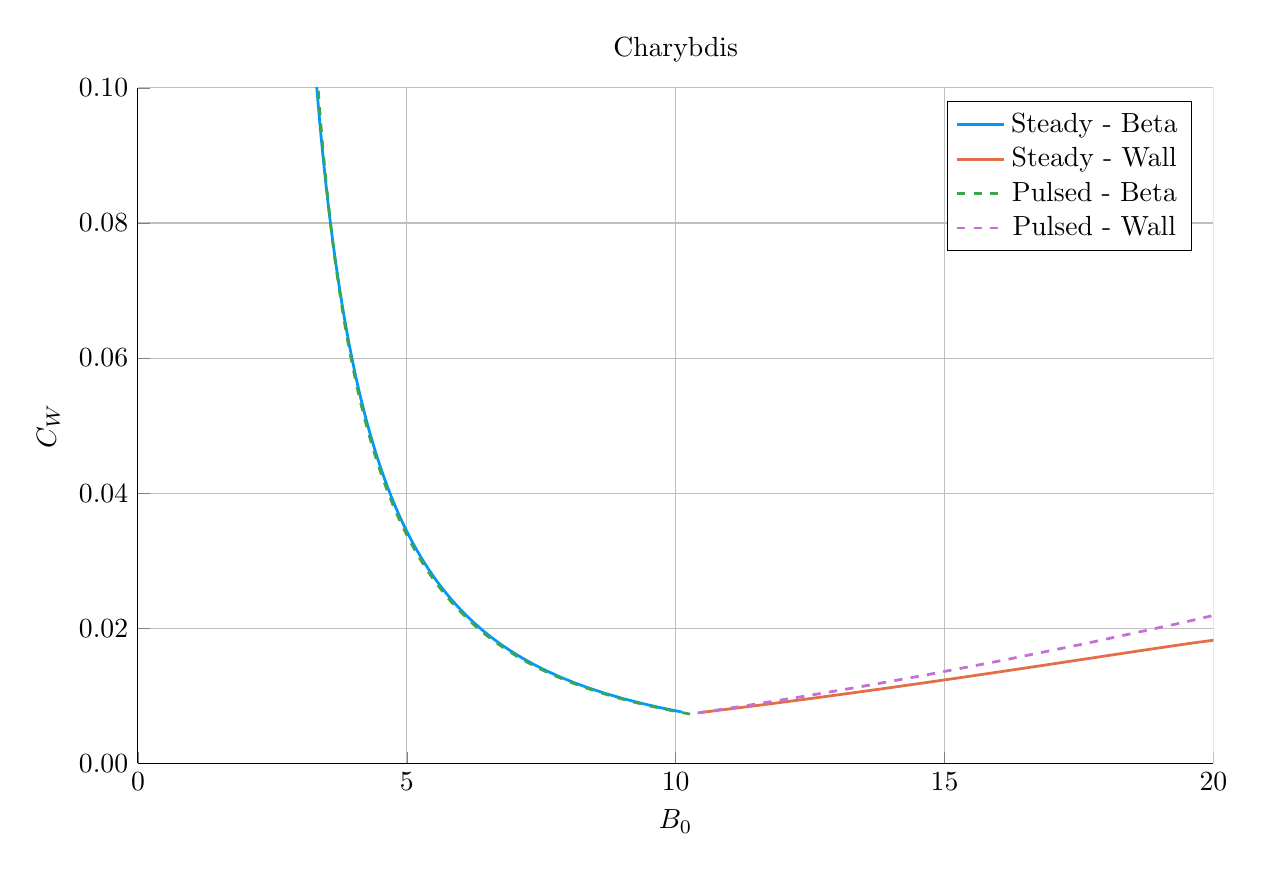
\begin{tikzpicture}[]
\begin{axis}[height = {101.6mm}, ylabel = {${C}_{W}$}, title = {Charybdis}, xmin = {0.0}, xmax = {20.0}, ymax = {0.1}, xlabel = {${B}_{0}$}, {unbounded coords=jump, scaled x ticks = false, xticklabel style={rotate = 0}, xmajorgrids = true, xtick = {0.0,5.0,10.0,15.0,20.0}, xticklabels = {0,5,10,15,20}, xtick align = inside, axis lines* = left, scaled y ticks = false, yticklabel style={rotate = 0}, ymajorgrids = true, ytick = {0.0,0.02,0.04,0.06,0.08,0.1}, yticklabels = {0.00,0.02,0.04,0.06,0.08,0.10}, ytick align = inside, axis lines* = left,     xshift = 0.0mm,
    yshift = 0.0mm,
    axis background/.style={fill={rgb,1:red,1.00000000;green,1.00000000;blue,1.00000000}}
, colorbar style={title=}}, ymin = {0.0}, width = {152.4mm}]\addplot+ [color = {rgb,1:red,0.00000000;green,0.60560316;blue,0.97868012},
draw opacity=1.0,
line width=1,
solid,mark = none,
mark size = 2.0,
mark options = {
    color = {rgb,1:red,0.00000000;green,0.00000000;blue,0.00000000}, draw opacity = 1.0,
    fill = {rgb,1:red,0.00000000;green,0.60560316;blue,0.97868012}, fill opacity = 1.0,
    line width = 1,
    rotate = 0,
    solid
}]coordinates {
(10.112818033153026, 0.007598383414978856)
(9.722156888543116, 0.008230424223188452)
(9.357875603858393, 0.008896404207575682)
(9.017653755630063, 0.009597023567402527)
(8.6995124437054, 0.010332804662622194)
(8.401566530516865, 0.011104394978990672)
(8.122163706328223, 0.011912345200844093)
(7.859819415455661, 0.012757161102175962)
(7.613196557650265, 0.013639302343912054)
(7.381088038653343, 0.014559181429827196)
(7.162401716104116, 0.015517162820285028)
(6.956147367527331, 0.016513562202290014)
(6.761425371986388, 0.017548645913683623)
(6.577416849463348, 0.018622630518712633)
(6.403375044688587, 0.019735682531644493)
(6.2386177769852695, 0.02088791828458706)
(6.0825208065966905, 0.022079403933712667)
(5.934511989185341, 0.02331015560822712)
(5.794066116682695, 0.024580139674436858)
(5.660700347012839, 0.02588927313954039)
(5.533970150598111, 0.027237424167073223)
(5.413465705416883, 0.02862441270831249)
(5.298808685607224, 0.03005001123436344)
(5.189649392059402, 0.031513945582432444)
(5.085664187259174, 0.033015895883282464)
(4.986553195072601, 0.03455549758379169)
(4.892038235455667, 0.03613234255000151)
(4.801860966679364, 0.037745980245626594)
(4.7157812114040425, 0.03939591897965519)
(4.633575445956479, 0.041081627216715676)
(4.5550354347559185, 0.04280253494397791)
(4.479966994069385, 0.04455803508845128)
(4.408188871204256, 0.046347484978679)
(4.33953172691477, 0.048170207844964834)
(4.273837210246432, 0.05002549435242988)
(4.210957116299974, 0.051912604161371986)
(4.15075261849161, 0.053830767509593334)
(4.0930935678432965, 0.05577918681155204)
(4.037857852672517, 0.05775703826940529)
(3.9849308127842145, 0.05976347349121981)
(3.9342047029103653, 0.06179762111185749)
(3.8855782007091695, 0.06385858841225403)
(3.838955955133626, 0.06594546293303978)
(3.7942481714200484, 0.06805731407868133)
(3.7513702293348077, 0.07019319470855978)
(3.710242331663442, 0.07235214271160313)
(3.6707891802306123, 0.0745331825613442)
(3.6329396770109583, 0.07673532684849063)
(3.5966266481325166, 0.07895757778829673)
(3.5617865887889004, 0.08119892870027327)
(3.5283594272686503, 0.08345836545794902)
(3.496288306480746, 0.08573486790664452)
(3.465519381509793, 0.08802741124736263)
(3.4360016318699595, 0.09033496738515884)
(3.4076866872513096, 0.0926565062404898)
(3.380528665662031, 0.09499099702224018)
(3.3544840229690007, 0.09733740946131986)
(3.3295114129297314, 0.09969471500383864)
(3.3055715568879336, 0.10206188796308927)
(3.2826271223788512, 0.10443790662966322)
(3.260642607548369, 0.10682175444066445)
(3.239584247604666, 0.10921242049746493)
(3.2194198921826622, 0.11160890156230109)
(3.2001189373344725, 0.11401020198268878)
(3.181652227422265, 0.11641533509457672)
(3.163991977015565, 0.11882332397376366)
(3.1471116955378684, 0.12123320224599504)
(3.130986116696265, 0.12364401485456963)
(3.115591132350856, 0.1260548187858383)
(3.1009037305081053, 0.12846468375306214)
(3.0869019371473265, 0.13087269283917113)
(3.0735647616124355, 0.13327794309901428)
(3.0608721453218655, 0.13567954612178545)
};
\addlegendentry{Steady - Beta}
\addplot+ [color = {rgb,1:red,0.88887350;green,0.43564919;blue,0.27812294},
draw opacity=1.0,
line width=1,
solid,mark = none,
mark size = 2.0,
mark options = {
    color = {rgb,1:red,0.00000000;green,0.00000000;blue,0.00000000}, draw opacity = 1.0,
    fill = {rgb,1:red,0.88887350;green,0.43564919;blue,0.27812294}, fill opacity = 1.0,
    line width = 1,
    rotate = 0,
    solid
}]coordinates {
(20.758867641064707, 0.018765308409143346)
(20.346250098246923, 0.018594952760163406)
(19.57104597888471, 0.01777146918538113)
(18.681781921115476, 0.016727851446155666)
(17.775790175980152, 0.015638576778075435)
(16.896654716492492, 0.014581653280825104)
(16.063927450323227, 0.013591211730165224)
(15.285557510665852, 0.012680275903338053)
(14.563500533069154, 0.01185123263968419)
(13.896568848875791, 0.01110114677254841)
(13.281970890030232, 0.010424581221258129)
(12.716170469467318, 0.009815118917575654)
(12.195372283741088, 0.00926617943914564)
(11.715794270833433, 0.008771443174384838)
(11.273815669498969, 0.008325054959037046)
(10.866051794088186, 0.007921704192505699)
(10.489365023931143, 0.007556609136513177)
};
\addlegendentry{Steady - Wall}
\addplot+ [color = {rgb,1:red,0.24222430;green,0.64327509;blue,0.30444865},
draw opacity=1.0,
line width=1,
dashed,mark = none,
mark size = 2.0,
mark options = {
    color = {rgb,1:red,0.00000000;green,0.00000000;blue,0.00000000}, draw opacity = 1.0,
    fill = {rgb,1:red,0.24222430;green,0.64327509;blue,0.30444865}, fill opacity = 1.0,
    line width = 1,
    rotate = 0,
    solid
}]coordinates {
(10.26788634689966, 0.007291637162809203)
(9.953967652326213, 0.007763018579561715)
(9.567926244368271, 0.008410560830066265)
(9.207974394987358, 0.009093056690349528)
(8.871841888699304, 0.009811202030777346)
(8.557505525932248, 0.010565644256199823)
(8.263156925406376, 0.01135697964954635)
(7.9871752024348766, 0.01218575089778548)
(7.728103682045175, 0.013052444820635726)
(7.484629973620137, 0.01395749030938975)
(7.255568856523303, 0.014901256485610468)
(7.039847526735421, 0.015884051087442074)
(6.836492834698909, 0.01690611908975986)
(6.644620209081183, 0.01796764156282338)
(6.463424013335149, 0.01906873477252413)
(6.2921691243175495, 0.020209449523749864)
(6.13018355681404, 0.02138977074682875)
(5.97685198655569, 0.022609617323612653)
(5.831610044919842, 0.023868842161338135)
(5.693939286027163, 0.025167232481888336)
(5.563362729090489, 0.026504510357656302)
(5.439440906144732, 0.0278803334592314)
(5.321768347746793, 0.02929429601917866)
(5.209970453003084, 0.030745929990983068)
(5.103700692769835, 0.03223470641747899)
(5.002638109938164, 0.03376003696406285)
(4.906485077678376, 0.03532127563010485)
(4.814965286571576, 0.03691772061565451)
(4.727821933804548, 0.03854861633202897)
(4.644816091323922, 0.04021315554278132)
(4.565725232806084, 0.04191048162126061)
(4.490341901840154, 0.04363969091085349)
(4.418472505906755, 0.04539983517396531)
(4.349936222622964, 0.047189924115870814)
(4.284564006352339, 0.049008927969770806)
(4.222197684694192, 0.05085578012965056)
(4.162689135592264, 0.05272937981792158)
(4.105899536872315, 0.05462859477526984)
(4.051698680949713, 0.056552263960658246)
(3.9999643482627323, 0.058499200250012214)
(3.9505817337017928, 0.06046819312273483)
(3.903442920928527, 0.062458011325916454)
(3.858446400032002, 0.06446740550676137)
(3.8154966244515616, 0.06649511080452623)
(3.7745036035252744, 0.06853984939399767)
(3.7353825273991994, 0.07060033297331114)
(3.6980534213689746, 0.07267526518964869)
(3.6624408270205375, 0.07476334399712868)
(3.62847350780097, 0.07686326394192533)
(3.5960841768845415, 0.07897371837037194)
(3.565209245407392, 0.08109340155652811)
(3.5357885893311605, 0.0832210107463015)
(3.5077653333614305, 0.08535524811591486)
(3.4810856504959875, 0.08749482264305544)
(3.4556985759109375, 0.08963845188964095)
(3.4315558340122845, 0.09178486369563649)
(3.408611677587535, 0.09393279778385825)
(3.3868227380888998, 0.09608100727612065)
(3.36614788616562, 0.09822826012150637)
(3.3465481016421226, 0.10037334043786662)
(3.327986352208224, 0.1025150497680155)
(3.3104274769652595, 0.10465220838353721)
(3.2938380965241474, 0.1067836557197021)
(3.278186482171801, 0.10890825269906537)
(3.263442495132517, 0.11102488135374605)
(3.2495774839156075, 0.1131324463411963)
(3.236564206241785, 0.11522987560063444)
(3.224376752844934, 0.11731612107126856)
(3.212990475972638, 0.11939015934381376)
(3.2023819222517877, 0.12145099224802183)
(3.192528769611062, 0.12349764737898258)
(3.1834097679780142, 0.1255291785649034)
(3.1750046834890777, 0.12754466627907632)
(3.1672942459724482, 0.12954321799866983)
};
\addlegendentry{Pulsed - Beta}
\addplot+ [color = {rgb,1:red,0.76444018;green,0.44411178;blue,0.82429754},
draw opacity=1.0,
line width=1,
dashed,mark = none,
mark size = 2.0,
mark options = {
    color = {rgb,1:red,0.00000000;green,0.00000000;blue,0.00000000}, draw opacity = 1.0,
    fill = {rgb,1:red,0.76444018;green,0.44411178;blue,0.82429754}, fill opacity = 1.0,
    line width = 1,
    rotate = 0,
    solid
}]coordinates {
(48.990476413653056, 0.09724163307501366)
(42.83950920694117, 0.07766994779263652)
(37.687790427214495, 0.06269593244609177)
(33.33937742845888, 0.05109841711622891)
(29.64296398154308, 0.04201539110057761)
(26.48039367255613, 0.034828857187910324)
(23.758442882319894, 0.029089432591006322)
(21.402860298405816, 0.02446606951047545)
(19.353987387634486, 0.020711961258999954)
(17.563502020363714, 0.017641064746807725)
(15.991970371213752, 0.015111701839397276)
(14.606987499719377, 0.013014953187280779)
(13.381751501116137, 0.011266342778060628)
(12.293960329570087, 0.009799811915435606)
(11.32495111804522, 0.00856330563618739)
(10.459023415380802, 0.007515507834648486)
(10.26788634689966, 0.007291637162809203)
};
\addlegendentry{Pulsed - Wall}
\end{axis}

\end{tikzpicture}

    \end{adjustbox}
        \caption{Toroidal Field Sensitivity}
    \end{subfigure}
    \hfill
    \begin{subfigure}[t]{0.48\textwidth}
        \centering
    \begin{adjustbox}{width=\textwidth}
      \Large
      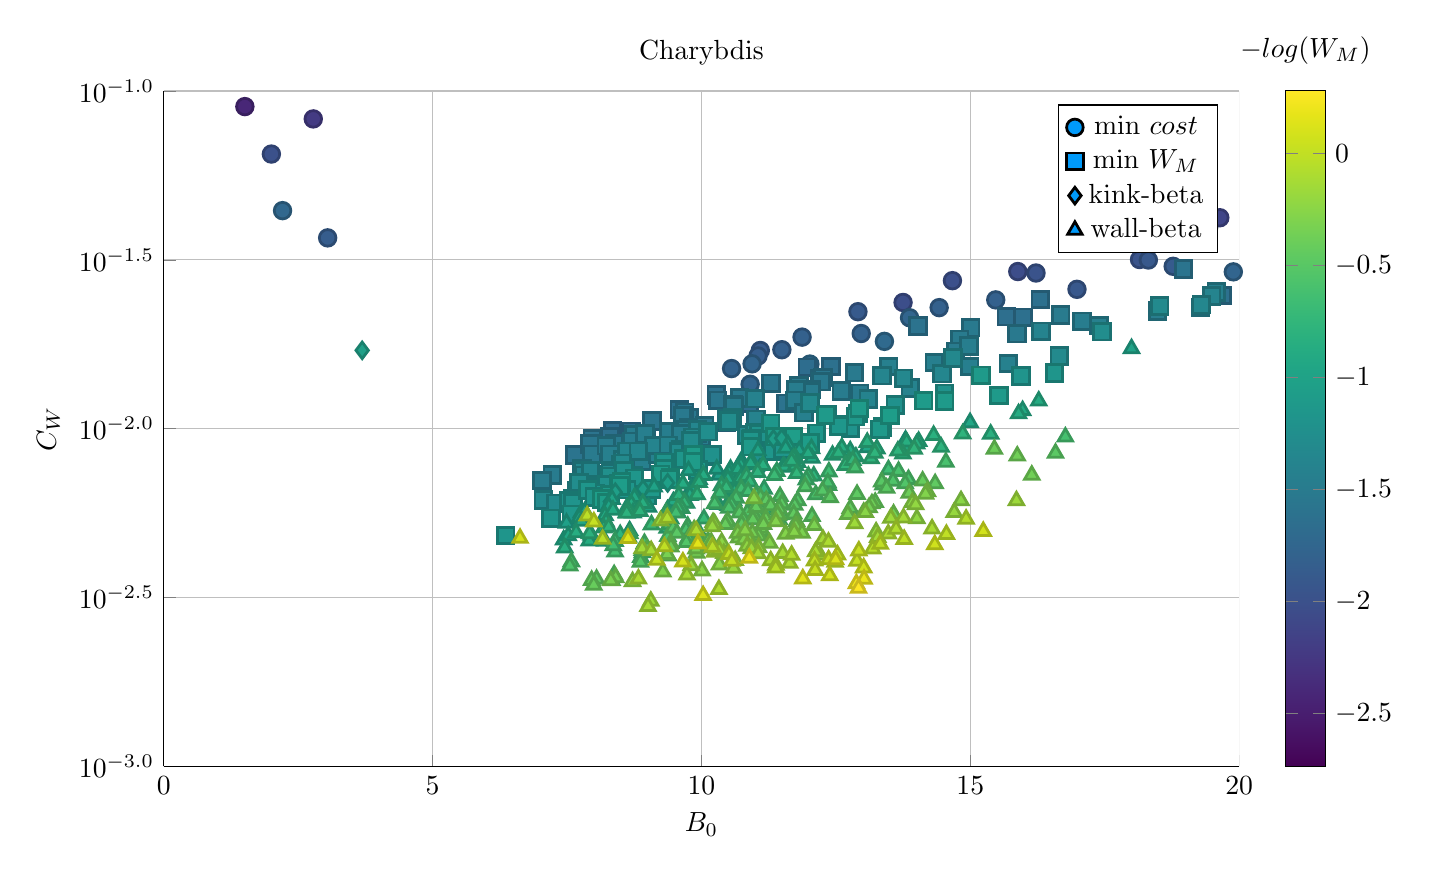
\begin{tikzpicture}[]
\begin{axis}[colorbar = {true}, height = {101.6mm}, ylabel = {${C}_{W}$}, title = {Charybdis}, xmin = {0.0}, xmax = {20.0}, ymax = {0.1}, ymode = {log}, xlabel = {${B}_{0}$}, {unbounded coords=jump, scaled x ticks = false, xticklabel style={rotate = 0}, xmajorgrids = true, xtick = {0.0,5.0,10.0,15.0,20.0}, xticklabels = {0,5,10,15,20}, xtick align = inside, axis lines* = left, scaled y ticks = false, yticklabel style={rotate = 0}, log basis y=10, ymajorgrids = true, ytick = {0.001,0.0031622776601683794,0.01,0.03162277660168379,0.1}, yticklabels = {$10^{-3.0}$,$10^{-2.5}$,$10^{-2.0}$,$10^{-1.5}$,$10^{-1.0}$}, ytick align = inside, axis lines* = left,     xshift = 0.0mm,
    yshift = 0.0mm,
    axis background/.style={fill={rgb,1:red,1.00000000;green,1.00000000;blue,1.00000000}}
, colormap={plots}{rgb=(0.26700400,0.00487400,0.32941500), rgb=(0.27794100,0.05632400,0.38119100), rgb=(0.28291000,0.10539300,0.42690200), rgb=(0.28229000,0.14591200,0.46151000), rgb=(0.27619400,0.19007400,0.49300100), rgb=(0.26514500,0.23295600,0.51659900), rgb=(0.25042500,0.27429000,0.53310300), rgb=(0.23360300,0.31382800,0.54391400), rgb=(0.21813000,0.34743200,0.55003800), rgb=(0.20123900,0.38367000,0.55429400), rgb=(0.18555600,0.41857000,0.55675300), rgb=(0.17117600,0.45253000,0.55796500), rgb=(0.15772900,0.48593200,0.55801300), rgb=(0.14618000,0.51541300,0.55682300), rgb=(0.13374300,0.54853500,0.55354100), rgb=(0.12346300,0.58168700,0.54744500), rgb=(0.11948300,0.61481700,0.53769200), rgb=(0.12632600,0.64410700,0.52531100), rgb=(0.15014800,0.67663100,0.50658900), rgb=(0.19109000,0.70836600,0.48228400), rgb=(0.24607000,0.73891000,0.45202400), rgb=(0.31192500,0.76782200,0.41558600), rgb=(0.37777900,0.79178100,0.37793900), rgb=(0.45867400,0.81636300,0.32972700), rgb=(0.54552400,0.83803900,0.27562600), rgb=(0.63690200,0.85654200,0.21662000), rgb=(0.73088900,0.87191600,0.15602900), rgb=(0.81457600,0.88339300,0.11034700), rgb=(0.90631100,0.89485500,0.09812500), rgb=(0.99324800,0.90615700,0.14393600)}, colorbar style={title=$-log( W_M )$}}, ymin = {0.001}, width = {152.4mm}]\addplot+[scatter, scatter src=explicit, only marks = {true}, color = {rgb,1:red,0.00000000;green,0.60560316;blue,0.97868012},
draw opacity=1,
line width=0,
solid,mark = *,
mark size = 3.0,
mark options = {
    color = {rgb,1:red,0.00000000;green,0.00000000;blue,0.00000000}, draw opacity = 1.0,
    fill = {rgb,1:red,0.00000000;green,0.60560316;blue,0.97868012}, fill opacity = 1,
    line width = 1,
    rotate = 0,
    solid
}] coordinates {
(43.17364371307109, 0.20372611777337152) [-2.737608795379803]
(36.93734773821979, 0.16756698485075783) [-2.687028959846787]
(48.32519073723288, 0.20307732356386315) [-2.590964172611572]
(27.818653653131317, 0.09697011319422226) [-2.5133293798402634]
(24.031609210800628, 0.08246486806905176) [-2.5100019193902536]
(46.9757183374081, 0.19848215388453824) [-2.5025824444647777]
(45.280165981821085, 0.18469850991270712) [-2.5011605733960924]
(34.33588556676648, 0.12156262800516612) [-2.487146433631915]
(49.350050230883724, 0.19851381203738652) [-2.4809660057819647]
(47.77223182347582, 0.18516332132320687) [-2.470276837036607]
(1.509009505191671, 0.08989325143911144) [-2.4120510478783452]
(1.607785753409308, 0.11208716242840429) [-2.40064821683863]
(36.7130287359324, 0.1197463715660703) [-2.3953673323479805]
(1.8837521570225992, 0.16126185747296792) [-2.393026566903574]
(40.03911031913926, 0.12157790627296668) [-2.3890711431592075]
(29.797147437037797, 0.08892691625963052) [-2.3841714318705525]
(49.837627165397436, 0.19098420146344375) [-2.3835230043455686]
(44.09667775143585, 0.1567069747417994) [-2.381290315955617]
(40.10027193508949, 0.12013460973440174) [-2.372431680776573]
(49.50704240080035, 0.18909730733563926) [-2.3528250340145016]
(28.968881363864583, 0.09075329244454268) [-2.3367870360584306]
(42.98831457790196, 0.14161197175057597) [-2.321478568273318]
(20.175934198309292, 0.05204568902739023) [-2.305558880403713]
(39.444164493588694, 0.12356138844469775) [-2.304074016625784]
(18.58289304393365, 0.04451265485552352) [-2.302767677581907]
(48.357898732015734, 0.16063854506387298) [-2.296827704935537]
(37.45895333311772, 0.10163604971512134) [-2.2875898578722627]
(38.208044910992896, 0.11621384520807569) [-2.277792210835674]
(48.821328515678495, 0.1663671711858832) [-2.2429196737605452]
(44.47436973980107, 0.14065371048755002) [-2.2307023150334016]
(36.201327387935265, 0.0992781716492562) [-2.229928759421221]
(24.976048511930994, 0.06165765133592798) [-2.225497521252979]
(2.781115265361342, 0.08264995845897197) [-2.2254079847151558]
(38.524798940282565, 0.10066936171865973) [-2.2222117952587324]
(40.75335661697331, 0.11283696845057267) [-2.2164511971368666]
(31.550557574122383, 0.07858675141449649) [-2.209080463460292]
(22.187409115367732, 0.055353669168383704) [-2.209072102647127]
(30.40343222814581, 0.08246628156983182) [-2.2082284492074966]
(22.891943050812795, 0.05534045927382465) [-2.207545754633005]
(32.48318348912026, 0.0812523499942961) [-2.2073960717358423]
(20.46108539491903, 0.04959003498021099) [-2.1906798686881843]
(24.303991155057293, 0.058916370946488036) [-2.180354292184896]
(20.69670598282277, 0.04458441983079472) [-2.1445063804884623]
(23.83667769146755, 0.05969099272190574) [-2.1441459472897755]
(19.63958505006771, 0.04213154094480493) [-2.1211539010866085]
(40.900769162095195, 0.11416954810746238) [-2.118865769548717]
(21.37751157855586, 0.04953083435602705) [-2.0989534800462293]
(33.36930679768429, 0.08867461574773429) [-2.098220502653117]
(24.013965403457117, 0.0528553369774306) [-2.0935531757786148]
(22.393434928615605, 0.05131047258257683) [-2.0908793980048204]
(29.571629059289982, 0.06966107994211436) [-2.071206080374841]
(20.977574074646927, 0.03996425224364798) [-2.064010547202469]
(18.060179054192336, 0.03708750697043753) [-2.056677518407323]
(35.94446843645834, 0.08410248770893317) [-2.046651526754166]
(15.882761260039363, 0.029196081498388402) [-2.0379011758864283]
(30.46355269165919, 0.07740613615195041) [-2.0346098603711273]
(13.74929111510663, 0.023645385119135078) [-2.0286798881208097]
(14.667163745602908, 0.027435451545116674) [-2.0136110022221563]
(40.970645504124256, 0.11225395679162868) [-2.009422091461703]
(18.86549676786543, 0.038038514881495206) [-2.0046094254929896]
(2.0018449519379766, 0.06504727548043324) [-1.9998626026906214]
(1.333016896105282, 0.1292818470624988) [-1.994011891463306]
(16.221280003397087, 0.028908830411030862) [-1.9684875514336135]
(18.146839242470875, 0.031694615819844695) [-1.962505769886516]
(20.536616448979608, 0.041976164443053174) [-1.9620022465602456]
(26.5908410355429, 0.0558374666834525) [-1.9556964151982232]
(24.564582250767256, 0.051180643617204404) [-1.951439472922028]
(19.431812066409112, 0.03938689654476367) [-1.9407104232831573]
(26.69111333219166, 0.05202238389928039) [-1.9285131737739916]
(16.98328208989546, 0.025864965787053298) [-1.9158089273231942]
(18.310414889815103, 0.0315876708787529) [-1.9026235632381945]
(23.297584692796203, 0.04007799426592172) [-1.8998797107494547]
(31.023963052023834, 0.06078277028813781) [-1.899469008660825]
(12.910038525246692, 0.022206649532263138) [-1.8922403969034376]
(41.62061738174131, 0.10343738795419383) [-1.8906275193753241]
(20.52842536101005, 0.03865878413437627) [-1.888904730447693]
(11.094220133483955, 0.01704724215883986) [-1.881726038777211]
(26.82066656529518, 0.05468787224768575) [-1.8763775212700056]
(35.10552519829791, 0.06894730353059726) [-1.8735628617782005]
(18.772509744848122, 0.030255781340376833) [-1.8728583861908288]
(27.360822192582077, 0.05616340524751281) [-1.8726476950037667]
(24.81797703498571, 0.04508699905590542) [-1.8707673950160981]
(3.0483538111563147, 0.036730885786441146) [-1.8559040168248113]
(29.522060018630928, 0.06072120698828991) [-1.844735439552174]
(39.46604489934323, 0.0887876180917983) [-1.8430067319432535]
(36.423170296938046, 0.06618962633184258) [-1.8418706711323614]
(11.051798631687303, 0.016421469596061083) [-1.839654971931263]
(25.458813886025002, 0.041749778425302704) [-1.8363695553529753]
(11.495131548398012, 0.017133631996777206) [-1.8261042714032643]
(32.71889711711922, 0.06559232169922954) [-1.8156007183182272]
(27.372160767771714, 0.050477285906930965) [-1.814915147975814]
(25.58270520703581, 0.0463768454249938) [-1.8142470512570916]
(14.420380568742246, 0.022826470712123872) [-1.8122133933822206]
(11.871194516454642, 0.018671308945999422) [-1.8120480447424478]
(15.472612894867664, 0.02406843511337114) [-1.810457309558868]
(20.542658667696518, 0.03627504764978015) [-1.8068853182048894]
(12.97099575986033, 0.019138039216325595) [-1.8019457667366159]
(21.252479627137433, 0.03724912279904193) [-1.7968505393892884]
(10.560232043643675, 0.015068032824050809) [-1.7952329403066731]
(45.12856703204009, 0.10460346899306477) [-1.7847262081815998]
(42.21258282310005, 0.09611727933154134) [-1.7840094275762153]
(13.869520871341438, 0.021310065419317785) [-1.76773605949338]
(19.89092632819806, 0.02913495659310822) [-1.7643358761825505]
(10.905382526033923, 0.013537430460188857) [-1.7636964772599824]
(10.941389456318912, 0.015563838196545969) [-1.7631697711543228]
(22.454106310710905, 0.039135813481222324) [-1.7625125196445544]
(30.835040451521607, 0.058991966200443106) [-1.7573515468471756]
(2.20974763812607, 0.04422563848495237) [-1.7287980416000448]
(38.02614384410885, 0.07767888704178068) [-1.7234251960549989]
(32.76556364087757, 0.06204137364185275) [-1.706346162862732]
(13.40240917641803, 0.018138423087163798) [-1.7045486732225623]
(46.55916074836906, 0.09124971330207729) [-1.7014359592573747]
(22.042270993490888, 0.0365316783828158) [-1.6927990438723723]
(12.016385149605648, 0.015536674756802697) [-1.6898457437353114]
(24.29682482728058, 0.04003550886686569) [-1.6732846842044926]
};
\addlegendentry{min $cost$}
\addlegendentry{min $W_M$}
\addlegendentry{kink-beta}
\addlegendentry{wall-beta}
\addplot+[scatter, scatter src=explicit, only marks = {true}, color = {rgb,1:red,0.00000000;green,0.60560316;blue,0.97868012},
draw opacity=1,
line width=0,
solid,mark = square*,
mark size = 3.0,
mark options = {
    color = {rgb,1:red,0.00000000;green,0.00000000;blue,0.00000000}, draw opacity = 1.0,
    fill = {rgb,1:red,0.00000000;green,0.60560316;blue,0.97868012}, fill opacity = 1,
    line width = 1,
    rotate = 0,
    solid
}] coordinates {
(11.967738248169791, 0.015197399614753464) [-1.6681264025020264]
(8.696464418773537, 0.009823451646161325) [-1.663027891651841]
(8.345089297998298, 0.009846202245989184) [-1.6574639825902946]
(10.880655338826603, 0.011920058291303071) [-1.6569597902573525]
(44.33631295480244, 0.07535163980234072) [-1.6567719329389001]
(15.669504585643491, 0.02145281320442147) [-1.6490985707391912]
(10.539028948810953, 0.010980468278747128) [-1.6422304847233504]
(16.300333423271717, 0.024120165421292625) [-1.6325751861823363]
(15.984439076117749, 0.021369208393676346) [-1.6291941426087102]
(32.92820758192895, 0.059322254561326254) [-1.6271960977249518]
(12.410293143428914, 0.015274978962504819) [-1.6270750467611084]
(19.688988499386202, 0.02479273110440336) [-1.626888156587228]
(47.183683314686505, 0.08930149237460469) [-1.6249314455189936]
(8.292561647347492, 0.009464726031912818) [-1.616950986036806]
(9.588347137721799, 0.01140193486941599) [-1.6155813119347568]
(8.006641138103518, 0.008812988458667981) [-1.6136190879018757]
(39.148691259933166, 0.06439016913414505) [-1.6120765470743166]
(10.27384306214681, 0.012585512817446045) [-1.6084381516776733]
(14.028211695717372, 0.02012839274260647) [-1.6020711217447665]
(7.943473491980901, 0.008960652359910951) [-1.5956625490662]
(11.571557791481624, 0.011885919211945236) [-1.5936419030965376]
(21.806471384188846, 0.03445722055743375) [-1.591719437101271]
(7.968648039596557, 0.00935259758229712) [-1.5882416690043395]
(8.97123185854356, 0.00941739351173858) [-1.587943800614445]
(7.642159237594249, 0.008359730036220061) [-1.5878025494857624]
(10.460983583083753, 0.010419937829338555) [-1.5868755906181577]
(18.965059522862617, 0.029697190504060857) [-1.5849823271963874]
(12.194568732238995, 0.014090253789926491) [-1.5820661333237485]
(9.813866298873991, 0.009872769680224545) [-1.571414774494934]
(24.25469890895016, 0.036055486397936085) [-1.561587842338199]
(8.517935684154212, 0.009008401602884603) [-1.5604752308741954]
(9.080862100268657, 0.010548811329102839) [-1.560024208321792]
(9.789660341943907, 0.00975086483062938) [-1.5595172183929409]
(8.133164457566973, 0.008877515881031174) [-1.5547403592804268]
(10.297704899446542, 0.012128004524771618) [-1.5525172912757694]
(9.766479902832291, 0.01075120106159998) [-1.550211325130473]
(12.2632951302657, 0.01417054313300387) [-1.5499921130488996]
(11.291662119925611, 0.013636547782905628) [-1.5488389310082484]
(9.686757381363082, 0.01118682853182229) [-1.548636584215126]
(7.924713370279235, 0.009004515948176011) [-1.5484303677563682]
(8.54226502879131, 0.008589361734950092) [-1.5300696832010154]
(9.64758141032686, 0.010918478084483) [-1.5240418415006989]
(12.21993539420707, 0.013786535741271849) [-1.52035115860342]
(15.867234965970042, 0.019102159289939535) [-1.5187095286365286]
(15.007125908258939, 0.019900882686515825) [-1.5152558703618486]
(10.70858947114034, 0.01233142370653334) [-1.5130633149050525]
(8.529805552034778, 0.008998649144966384) [-1.5127417843169062]
(8.377294862413901, 0.009033035828776036) [-1.512065872282441]
(12.846715954681153, 0.014648425212785676) [-1.508698938344436]
(16.682126583618288, 0.021717369003602268) [-1.5042599211378067]
(10.58390997110411, 0.011787983533386965) [-1.5034350531454859]
(11.810966417691285, 0.013402736400337721) [-1.50170709764633]
(7.965952597674263, 0.008403497514698337) [-1.501622468932281]
(12.052123659751864, 0.013038942564365743) [-1.5014482706318735]
(14.803678461986678, 0.018390392389316428) [-1.4999954524234758]
(14.727306928855038, 0.01694354359189593) [-1.4973617780251773]
(10.061864920509048, 0.010183371556613061) [-1.497105465512374]
(40.24136746900709, 0.062282935043912684) [-1.4929511344473714]
(41.49663881325739, 0.06324187033686292) [-1.4921349419619385]
(11.804455973082419, 0.012548762978995496) [-1.4884591559674822]
(12.029939715648373, 0.012867101009559307) [-1.487363796795517]
(12.601637635718813, 0.012921001622500157) [-1.4866917975345906]
(9.754197703405268, 0.010047951074758055) [-1.4840978906845892]
(21.882416551144317, 0.03303866433608294) [-1.4824521913249147]
(12.942504869667264, 0.012726704506142847) [-1.4821332841886103]
(7.226740691315094, 0.007290805739373347) [-1.48122389777201]
(9.72526998487911, 0.00977012454088988) [-1.4804970319589599]
(7.032760703447595, 0.007020834402326414) [-1.4800609203732897]
(8.228283040534254, 0.008910343679206711) [-1.4785263901161534]
(11.757080569358145, 0.013060328514041545) [-1.4759327339004988]
(8.742108415330497, 0.009568901799246174) [-1.4716802129865878]
(10.608355718332808, 0.011686646580567617) [-1.4714171457200942]
(10.002017917096252, 0.009432683201513142) [-1.4697490463241623]
(17.076056816605465, 0.0207896268155257) [-1.469182095495403]
(9.93096524460024, 0.00970055448692835) [-1.4669160574764228]
(9.646537177073283, 0.009906198335664992) [-1.4650279037766998]
(8.492788974520707, 0.008175296861755412) [-1.4649157170050158]
(39.01795702656691, 0.06304537805517052) [-1.4637589731711664]
(37.319780376430465, 0.058293696935902015) [-1.4637269213699509]
(18.482121616159016, 0.022332692478256824) [-1.4633431723635995]
(8.698182291263416, 0.009175072172052877) [-1.4625771233357587]
(28.127107238558466, 0.03507245292213848) [-1.4624493219359893]
(24.405556044324065, 0.0323252483349636) [-1.456137936078477]
(11.740431759483823, 0.012144991566364045) [-1.4552956920106896]
(9.39566274467647, 0.009807429458519862) [-1.4545765412204814]
(14.971887946904854, 0.017552109366812733) [-1.4536933205355047]
(8.340793691955412, 0.008376880643338882) [-1.4536264367612777]
(20.758621662871732, 0.027928446404318328) [-1.4522195766945736]
(14.989566420933915, 0.015275332383460013) [-1.4474663709891824]
(14.328449262483707, 0.015700047070746036) [-1.4473086055649607]
(9.614108815012006, 0.009670159078421467) [-1.4394573389116623]
(8.946816680478415, 0.00966580645268258) [-1.43910869750835]
(17.39032103778615, 0.02020398851625505) [-1.4359212547397637]
(8.887301811416945, 0.008025741974410725) [-1.4345455569874563]
(8.293678413022477, 0.008395971364345037) [-1.4342039611389994]
(34.870157215661116, 0.055516720625521446) [-1.431939711468657]
(9.215949656599236, 0.008564631451482608) [-1.4318393301192203]
(13.483733389139449, 0.015286328537971657) [-1.4298782830268841]
(11.909294643223976, 0.011144326549623773) [-1.4297531319990848]
(19.28479299500749, 0.022836013108600235) [-1.429493152311542]
(19.574343065749268, 0.02541733792453219) [-1.4257656907023994]
(7.775559573362513, 0.007637958943877289) [-1.4246908118870814]
(25.190615990519625, 0.032702505993041836) [-1.4223151615986427]
(15.706222639321235, 0.015605848032644089) [-1.4209285260987674]
(9.186736487920959, 0.00838874188644035) [-1.4103191250155003]
(7.810243176708771, 0.007287678962320866) [-1.409160412241362]
(10.994509564269785, 0.012263516831132143) [-1.3987487890322283]
(11.014663159593116, 0.010656632838165833) [-1.3961077718749653]
(13.882977876787413, 0.013186567390631069) [-1.39553831950318]
(9.36196654538676, 0.00805251109990194) [-1.3921916689745937]
(16.3128197434878, 0.019423304332311736) [-1.391977480132208]
(21.05130093390351, 0.025114205055596032) [-1.3910450519688433]
(21.18381811006707, 0.026458278303411537) [-1.3854794296349102]
(13.100755547904486, 0.012247975078154037) [-1.3835251244626703]
(9.120715613380417, 0.008921077760690099) [-1.3812630274600655]
(7.896894254399229, 0.007416332681742631) [-1.3791460184166777]
(9.381274310380604, 0.008932161350486465) [-1.376877777579119]
(19.488100600993267, 0.024683476432383993) [-1.375791428631395]
(10.475402655568338, 0.010670268336180793) [-1.3747828318073587]
(9.32515552589659, 0.007870433585163046) [-1.3692376523933565]
(7.9286970308329465, 0.0074378152848894735) [-1.3684330757581267]
(8.538214357510187, 0.008098566001726598) [-1.3642308788975135]
(13.354119232582212, 0.014345667909698757) [-1.3639106630352087]
(8.608422674568363, 0.008572986953587419) [-1.3552608297970883]
(9.925761115396522, 0.00992037446225701) [-1.3550143961305745]
(8.004082331921554, 0.007328347073490059) [-1.3536632792649093]
(7.802422783894211, 0.007510901593863939) [-1.3520272957429909]
(14.471041037539871, 0.014541602438699657) [-1.3510576974042412]
(7.810600769649848, 0.007284218364658594) [-1.3496042220443973]
(19.296422276685288, 0.023274179527198832) [-1.341589260669594]
(8.824939461101431, 0.008576558289309913) [-1.3400141478767358]
(8.49764138867205, 0.00783880949696723) [-1.3300314493551002]
(13.758392145064837, 0.01411038207207742) [-1.3284263237560021]
(7.937511343586117, 0.007486503783717723) [-1.3242939338468662]
(14.679707952711722, 0.016172436730796002) [-1.323178727777929]
(8.319781298347303, 0.007515284989600465) [-1.3213550729926942]
(27.500324284476235, 0.031083172357107024) [-1.3188753969554132]
(7.672777169827471, 0.006572813918743706) [-1.3138992633454782]
(34.26204390685552, 0.04309583371292883) [-1.3112533972207423]
(8.305241116382918, 0.007413444843148486) [-1.3066175516543825]
(18.522037273131268, 0.02306836377257982) [-1.3040612288627607]
(9.843274954742599, 0.00943254285754032) [-1.3038133693852783]
(12.01595379328233, 0.01190899263404481) [-1.301084703290134]
(8.530188695097733, 0.00789699984651379) [-1.3010145120900876]
(7.059381386127842, 0.006149219434619409) [-1.3000605956773916]
(16.655180883583878, 0.016437005811172183) [-1.2981699890610565]
(9.606246685298759, 0.008660055713531614) [-1.2951558801969907]
(10.571439501867458, 0.010749954823506654) [-1.29444309797184]
(7.284894188691189, 0.006015009649024556) [-1.2856101424882644]
(10.842752178226151, 0.009584357937856927) [-1.285263592011844]
(34.353143867925155, 0.04494124949431044) [-1.284383793501614]
(7.905156667937178, 0.00683431321635412) [-1.2828114288158374]
(31.635765029342274, 0.039187382342347976) [-1.2826431650359629]
(8.313601928775393, 0.007231700278305266) [-1.2824255065429995]
(9.578913894726805, 0.00853616645957665) [-1.2813323109549335]
(7.924882086401339, 0.006837657402697755) [-1.2806421539894215]
(9.808329366529762, 0.009211465915111147) [-1.2790915578265545]
(10.511748242466084, 0.010542099378207213) [-1.2707451840708122]
(23.70716861300546, 0.024447750750697092) [-1.2676539939434082]
(11.00520478529279, 0.009098409772603787) [-1.2653553126366786]
(7.876105123562427, 0.006725537497980498) [-1.264293982211982]
(17.45204956258683, 0.019363431367524053) [-1.262045130852001]
(7.719844293445014, 0.006906076996276599) [-1.2611290819783112]
(10.118399421716713, 0.009803145458874337) [-1.2555987795426622]
(7.612390232156273, 0.00619895569247597) [-1.2513270179335647]
(8.729387536492673, 0.007239853513876978) [-1.2453167838780697]
(10.961169543919764, 0.008896586162085272) [-1.2430939343579344]
(10.985358154781366, 0.009719593902466845) [-1.2381773742332136]
(10.055825077383927, 0.008270424440644015) [-1.2346782486332617]
(8.291481327682558, 0.0072241626571935376) [-1.2264046023709216]
(12.335638193913455, 0.01098843719538726) [-1.2247195887884887]
(8.246208566536797, 0.006808974225612837) [-1.2180889658059086]
(8.540264952931636, 0.006611305121542242) [-1.2173874089477876]
(8.556190004184526, 0.007501419726936573) [-1.2146247722956514]
(13.602894240173864, 0.011764386053045915) [-1.2132972156104522]
(10.195221885432844, 0.008378063320530003) [-1.2109120215395388]
(11.049738848862685, 0.008427299987451904) [-1.2084181738286368]
(14.519807280009873, 0.01273555061242485) [-1.20714909048448]
(12.595222602654314, 0.010213320377511352) [-1.2033520253557135]
(26.383495577820405, 0.032086426450625864) [-1.1973567207367808]
(12.639134913781255, 0.01024990923611188) [-1.1946911954531152]
(12.771017041564328, 0.010020735618058307) [-1.194687477055283]
(11.065493657555185, 0.009634752809511687) [-1.1937967228670217]
(15.93895045303613, 0.014319974319254046) [-1.185724861965876]
(28.62771924607459, 0.030946696104817876) [-1.1815951507377263]
(7.535456478096903, 0.006119538485938838) [-1.1806237088701466]
(7.610400378886139, 0.0060467130253046425) [-1.1800813312023146]
(9.303943294896706, 0.007952378649071718) [-1.176244530950471]
(8.033169581940832, 0.006432608194369421) [-1.1748225292203367]
(7.199323628519372, 0.005427058328431804) [-1.1721208310483742]
(8.635658099111911, 0.006744537821609478) [-1.1717373686057835]
(6.357367087501427, 0.004828891223049449) [-1.1708649361692889]
(8.68097527641003, 0.006810003648499363) [-1.1692163263768098]
(10.941107168878954, 0.009353534353065332) [-1.167353919317699]
(16.564321004099757, 0.014618785296867573) [-1.1652399164280889]
(11.54197585545895, 0.008829535690276422) [-1.162809974145342]
(8.753893841415247, 0.007136024429485349) [-1.1600693635040116]
(7.885243678455898, 0.006579111152003091) [-1.157321108695414]
(11.32266327338597, 0.008599780741533768) [-1.1572067562856314]
(10.915418141745553, 0.009251618906581017) [-1.1571634670399211]
(9.667898706541429, 0.008133610271699837) [-1.154357334346231]
(12.910014006891455, 0.011084851654264415) [-1.1506586644938104]
(11.51111009989439, 0.008713510430388705) [-1.150227655836216]
(8.60996222930752, 0.006602548762005154) [-1.1491924102402016]
(8.006315067088401, 0.006272419326365313) [-1.1477835171917188]
(9.30257761823372, 0.007620679601131938) [-1.1465058315496728]
(11.285570988608995, 0.010377192915174936) [-1.145014274974487]
(12.138687953769608, 0.009696220536212618) [-1.1375870233869183]
(12.553842085049038, 0.010180634102852183) [-1.1373650551215082]
(9.934623605013899, 0.007542730978334406) [-1.1357458790371815]
(13.364635095205022, 0.010126349397671063) [-1.133986432515703]
(7.577912363275431, 0.005578205050921048) [-1.1320341014158335]
(12.86501420031779, 0.010846318354017281) [-1.127079592692178]
(8.98804676924596, 0.006331906889150134) [-1.1252988863479554]
(8.452377355502822, 0.006879141460401252) [-1.123003263844327]
(23.025824780010147, 0.022040928898795047) [-1.1207682191899027]
(13.322832437569058, 0.00996173564893061) [-1.1180749050851169]
(9.076598934998714, 0.006626896988025552) [-1.1159299024060154]
(15.198462033251472, 0.014399132022875615) [-1.111366047368976]
(14.521859369334845, 0.01206983625295502) [-1.1093461418096882]
(8.297041065786505, 0.006356432017833017) [-1.1083223146390213]
(15.534651072689927, 0.012535144034281957) [-1.108020004377878]
(10.912955767488512, 0.00883860338226376) [-1.1055395253528022]
(12.308396510673756, 0.010954609847675004) [-1.1018087579792433]
(8.515520072517582, 0.006955673427821012) [-1.1000312304906807]
(12.935222387807004, 0.011476323196829152) [-1.0958683903566835]
(14.133023152666118, 0.012099180088161502) [-1.0918611830445206]
(9.240930260616448, 0.007324655445979312) [-1.084008635561983]
(9.850752183763255, 0.008347799057721199) [-1.0818442729737123]
(9.835917844908545, 0.007973263522900845) [-1.0762205003226006]
(13.503659427877482, 0.010946001598484297) [-1.0742112770850791]
(12.015541559387604, 0.009087852412631436) [-1.0708769548182164]
(8.48180872327906, 0.0067597442860644836) [-1.069695292943837]
(9.426016311012596, 0.007160447099405331) [-1.0603710996179994]
(11.370815749528317, 0.009473258949863166) [-1.058639833713732]
(8.145331814193963, 0.0061899243692649306) [-1.0559914680496412]
(11.710887773696074, 0.009482529791919412) [-1.0537452246128203]
(9.401232433154894, 0.00708059455566661) [-1.0532767994986825]
(8.244715434296548, 0.006035560775312132) [-1.0518252532905286]
};
\addlegendentry{min $cost$}
\addlegendentry{min $W_M$}
\addlegendentry{kink-beta}
\addlegendentry{wall-beta}
\addplot+[scatter, scatter src=explicit, only marks = {true}, color = {rgb,1:red,0.00000000;green,0.60560316;blue,0.97868012},
draw opacity=1,
line width=0,
solid,mark = diamond*,
mark size = 3.0,
mark options = {
    color = {rgb,1:red,0.00000000;green,0.00000000;blue,0.00000000}, draw opacity = 1.0,
    fill = {rgb,1:red,0.00000000;green,0.60560316;blue,0.97868012}, fill opacity = 1,
    line width = 1,
    rotate = 0,
    solid
}] coordinates {
(8.305244154675892, 0.006083501631057066) [-1.0496814932160978]
(8.913067820493207, 0.006629793134010975) [-1.0478282176510978]
(11.088375868477236, 0.00764908073743482) [-1.0476862508436227]
(8.893467896647309, 0.005862884354721373) [-1.0434060376287386]
(11.339319277973114, 0.009322710512378526) [-1.042586757918211]
(8.397189975968995, 0.006487752068877104) [-1.0395059774095508]
(11.489774589946819, 0.009374281366493263) [-1.037130039873791]
(3.690186058729787, 0.0170614588554745) [-1.0308313508546258]
(9.371675394558984, 0.006913114243597262) [-1.0275590312193816]
};
\addlegendentry{min $cost$}
\addlegendentry{min $W_M$}
\addlegendentry{kink-beta}
\addlegendentry{wall-beta}
\addplot+[scatter, scatter src=explicit, only marks = {true}, color = {rgb,1:red,0.00000000;green,0.60560316;blue,0.97868012},
draw opacity=1,
line width=0,
solid,mark = triangle*,
mark size = 3.0,
mark options = {
    color = {rgb,1:red,0.00000000;green,0.00000000;blue,0.00000000}, draw opacity = 1.0,
    fill = {rgb,1:red,0.00000000;green,0.60560316;blue,0.97868012}, fill opacity = 1,
    line width = 1,
    rotate = 0,
    solid
}] coordinates {
(7.490392990216207, 0.005256053052710575) [-1.025114084474608]
(10.324607857349502, 0.007284527271346537) [-1.025064662372027]
(10.786179524347823, 0.00782078493256419) [-1.0135716419780334]
(8.265254899703113, 0.005878041854646887) [-1.0133032391552028]
(9.759627120315386, 0.007516810149579491) [-1.0129395602075102]
(7.765989799277702, 0.005642606316680264) [-1.0090683465802397]
(10.284485653997232, 0.007590586049588419) [-1.00487994972194]
(10.740566234689192, 0.008018904893245096) [-1.0024486517409639]
(7.82952747253988, 0.005687012650490601) [-0.9982503197852052]
(17.997767505161434, 0.017272851302606376) [-0.9980863049007114]
(11.607406337271188, 0.008976011549139531) [-0.9976413099828907]
(9.120664508219399, 0.00672377146821775) [-0.9952427135597887]
(8.33813410692626, 0.006179152610909006) [-0.9882704184280687]
(9.809381065883368, 0.006658577387207133) [-0.9865959618907963]
(11.05015741923656, 0.008611185683760977) [-0.9861502224644026]
(11.81726987578575, 0.00861006159819778) [-0.9834884062410291]
(9.955965615750785, 0.007078972975952707) [-0.9755470230412873]
(10.468778589579204, 0.007165169234302644) [-0.9751682968759733]
(8.275975247764718, 0.00588288059860778) [-0.9745460269854277]
(11.56641933994839, 0.008762707263760248) [-0.9724510296030006]
(7.729666360230168, 0.0054508764537053) [-0.9721723790112873]
(10.728788856458863, 0.007500206088288035) [-0.9683079871351761]
(13.794818258324069, 0.00925430650881406) [-0.9640479639625688]
(10.68702976676658, 0.007713542274813112) [-0.9605456904465843]
(13.086397858972267, 0.008793232884908199) [-0.9509475064598062]
(10.540636515545728, 0.00758530046831779) [-0.9475613034981963]
(14.994597091286334, 0.010432599107525612) [-0.9431073279051986]
(10.771912405971477, 0.006669463740427501) [-0.9395228095882537]
(7.437916255626304, 0.004688262944849126) [-0.9379797386819722]
(9.01626097658872, 0.005855680709409532) [-0.936956260188316]
(7.522698377806809, 0.004823068577046762) [-0.9328401416066296]
(8.754915642687301, 0.006257853989784519) [-0.9307108052550614]
(10.594981119045784, 0.006461854726339168) [-0.9281558619803609]
(12.045885329425058, 0.008735963170322575) [-0.9264995775599043]
(7.771430799983934, 0.005328057424477724) [-0.9262426999191099]
(10.735292233144142, 0.007790932759723544) [-0.9227003718927437]
(10.512921169293449, 0.007406866683715918) [-0.9211202387251416]
(7.950782637474951, 0.004842693465206878) [-0.9122780994598872]
(8.205592174769814, 0.00553456744660005) [-0.9098639973117462]
(10.931685642752342, 0.00799774423691871) [-0.9085892171866993]
(15.972145415340275, 0.011322447729645281) [-0.9043705523492929]
(12.054696727590375, 0.008178982728725071) [-0.903352069757217]
(8.649488124233137, 0.0058981820527739225) [-0.9005612951337819]
(9.785411486209819, 0.006353815969057234) [-0.8985196847828957]
(8.355237320864756, 0.005739892493181049) [-0.8983797144291398]
(10.676348105658398, 0.007583618995886536) [-0.8971261027713628]
(9.478163505938792, 0.006081355532545074) [-0.8962149920198969]
(10.912879849760056, 0.007895141300507174) [-0.8947574466288085]
(11.983353362889243, 0.008446442250875192) [-0.8916300803179569]
(16.272383561884997, 0.012086236110976131) [-0.890947883956792]
(11.52098349265942, 0.007728598763745398) [-0.8865999168444305]
(10.536757160705346, 0.006968625853256571) [-0.8862290860463612]
(9.655565692459556, 0.00686791587727973) [-0.8853692596179883]
(15.897115425748877, 0.011077289150155845) [-0.884029767456243]
(8.695755457607955, 0.005982150284429834) [-0.8837850767800522]
(10.492158100051922, 0.007098671990886852) [-0.8828563557879437]
(10.037701951865458, 0.0072796273438267495) [-0.8804549747402444]
(11.638039502619437, 0.007792003070402551) [-0.8799662830695792]
(11.546710974717332, 0.007704064980519725) [-0.8744133357565225]
(8.726391874140708, 0.0056363780626130485) [-0.8730986298376362]
(8.663680556671139, 0.004988178616679241) [-0.8728030894608018]
(13.787374648539751, 0.008770502666972253) [-0.8727320299344076]
(12.766608989345242, 0.008601244202966506) [-0.8720334149277572]
(7.912625943172549, 0.004655770362479482) [-0.8693487943882443]
(10.513846731080314, 0.006084065906903396) [-0.8630202034214742]
(7.669338719372169, 0.004924842040843803) [-0.861299793442028]
(8.225117880579704, 0.005298172414294102) [-0.8595038240809204]
(8.203452347735475, 0.0046473625238345456) [-0.8567854750862633]
(8.606501005951438, 0.005815101976145971) [-0.8560196956809655]
(12.610505281824743, 0.008787976150626518) [-0.8549409997795642]
(8.607112161141583, 0.005657937584887749) [-0.8549130093089008]
(14.038960987293587, 0.00917703801839012) [-0.8535716907113037]
(12.43732861090992, 0.008347881751030625) [-0.8521148893133685]
(10.730288560624734, 0.007128967537191795) [-0.848258534769848]
(13.814182568957458, 0.009136355586300991) [-0.8460593767435973]
(10.614949449057972, 0.006518603909074656) [-0.8436096023361083]
(8.910346704261844, 0.006010163492689091) [-0.8427994583004987]
(11.789269747471279, 0.007945945585113466) [-0.841947416622939]
(9.721588138355992, 0.0060248058000312785) [-0.840612447094069]
(7.4570907362874745, 0.004440943928455613) [-0.840512586473128]
(11.749954066883152, 0.008192611227802852) [-0.8396933257766793]
(11.145583374518681, 0.007794162811523137) [-0.8357637262102798]
(14.002098633144497, 0.009012091589396549) [-0.8345082268411569]
(11.71396125221291, 0.008170154991858254) [-0.8326261675235949]
(9.954982275936574, 0.006937374865533122) [-0.8320882392153445]
(9.368409582792285, 0.005749714926123568) [-0.8315762378530004]
(10.476236084679716, 0.00662694635784487) [-0.8307347851507457]
(15.378598226574077, 0.009642717688792466) [-0.830544413041331]
(12.871582541696636, 0.008249655917762508) [-0.8297213382977437]
(13.261596482506313, 0.00872151277844613) [-0.8286741188165131]
(13.0829776821363, 0.009115953893059449) [-0.8267848509238259]
(14.317311822247486, 0.009559156785738465) [-0.8225460718617404]
(8.639262951926671, 0.005739050504125615) [-0.8214723162104086]
(11.749576633189198, 0.00777900336077081) [-0.8201412806434945]
(12.546153140118335, 0.008465745314703852) [-0.8151576039795889]
(8.183555235334351, 0.005082760625336129) [-0.8142249848207472]
(11.675608431762104, 0.008019437945510303) [-0.8140641213229001]
(10.313233660105723, 0.005973868428211905) [-0.8103019758142813]
(7.919842291864804, 0.0048937089468515296) [-0.8012431956657198]
(8.609864055202394, 0.005621145192877696) [-0.8003481799777136]
(9.57863964924036, 0.006353153460386551) [-0.7977579467571502]
(13.746798877450388, 0.008421833334043108) [-0.7930251215824343]
(11.044783092119218, 0.007429093264895125) [-0.7890451923079399]
(14.456103371629998, 0.008826772268823495) [-0.787865286509519]
(9.919321037115749, 0.006383916218566666) [-0.7843040366780064]
(8.854683142750217, 0.005696794743220581) [-0.7839186276792087]
(10.597279263558937, 0.006115696804857897) [-0.7832803335041352]
(9.426262484951625, 0.005413509713037376) [-0.7821184247172652]
(13.65357832167086, 0.008596617727968549) [-0.7805782205003577]
(14.85793053450062, 0.009659872283801132) [-0.7798419979328133]
(13.154203573323626, 0.008159117975808313) [-0.779526126485372]
(12.747830729091781, 0.00801636696090187) [-0.7754633993416067]
(13.223550772820014, 0.008468144805643287) [-0.7736782567370082]
(12.088805642739427, 0.007247388825611958) [-0.7730881104428101]
(8.488492913699757, 0.004861686496363432) [-0.771875090323587]
(10.495316608073319, 0.005934301325116477) [-0.7684162906476206]
(9.362567206766446, 0.005077595748671911) [-0.7679743247932476]
(10.372000769339135, 0.006786674226710283) [-0.7648185888526707]
(8.27284371455478, 0.005109733182186724) [-0.7640789887074095]
(13.955087628156079, 0.008706119585241447) [-0.761342175922955]
(10.544958602900675, 0.005941882664679825) [-0.7543127087245246]
(11.77031037870365, 0.007371584809935278) [-0.7536484511278393]
(10.836697344568485, 0.007235631321785017) [-0.7503956953450397]
(12.6755982178082, 0.007794584633403252) [-0.7487808552191573]
(12.814719377106297, 0.008059650365173391) [-0.7476061772087611]
(10.900321708767143, 0.006963610302502873) [-0.7471256555265617]
(10.461287221109892, 0.006698880656946609) [-0.7413304463691416]
(9.558670032438643, 0.005641975327508916) [-0.7367054574686347]
(9.682364623465833, 0.006032870871331476) [-0.7331219552552337]
(11.16543967690182, 0.006626912607429937) [-0.7143600945963312]
(11.401694656436039, 0.007474831733495699) [-0.7106398428950327]
(9.939172881280367, 0.0049761893476396495) [-0.6960873863412442]
(10.046704529687267, 0.005409555517719824) [-0.6958903955949629]
(11.07309218913271, 0.005844386265058715) [-0.6930492540076382]
(9.631413377269118, 0.00580869705512685) [-0.6929516890222392]
(9.0705472826982, 0.005195474212399125) [-0.6915921881710438]
(10.340119383327263, 0.006450299363758911) [-0.6857195379800745]
(11.988661863115587, 0.007235955498415392) [-0.6856480650317041]
(11.356954793810704, 0.007277002386326683) [-0.6825231692879921]
(9.559961062893178, 0.005826409813708321) [-0.6799325504597861]
(11.1835890784689, 0.005748438997690529) [-0.6756496749536086]
(8.391628360065997, 0.004642372121698665) [-0.6668421547656437]
(11.949965044033023, 0.0070613972149505) [-0.6594486343899455]
(9.397214543064022, 0.005204006670639966) [-0.6592191769587943]
(10.74094896614302, 0.006638640066368149) [-0.6536209377575128]
(13.476998824812561, 0.007561107269230883) [-0.650948550154174]
(12.36964710930465, 0.0074536379991662315) [-0.6505954513533947]
(9.341639857223466, 0.00562511440860501) [-0.649384718466127]
(9.524994554706348, 0.0056379604361593005) [-0.6434610863211887]
(8.667648129644444, 0.004893302789367808) [-0.6386314300711667]
(10.86703111417762, 0.006520915492483144) [-0.6385156325462752]
(8.903387056823963, 0.004295648023998173) [-0.6376426431852426]
(8.39310786606612, 0.0043195416112934695) [-0.63745836942971]
(8.35978027986981, 0.004504479712425151) [-0.634161727858793]
(11.107940679063978, 0.00550347046899009) [-0.6307004133850902]
(12.85647542381142, 0.0076645781815444635) [-0.6183303859395417]
(8.639519611289709, 0.004777548127961022) [-0.6130870829164431]
(9.745180550219304, 0.005139848231321853) [-0.6129648030838463]
(16.767571242014334, 0.009455939774823839) [-0.6084696230229766]
(10.246078544026743, 0.005998204689845081) [-0.6069152599086628]
(10.644474286152628, 0.006234008404953501) [-0.6054076068022625]
(10.558536641296014, 0.005960524285263344) [-0.6024296737568321]
(8.8713583098509, 0.004158248718194877) [-0.6015484963981724]
(12.361855328211519, 0.006792484353594769) [-0.6012984238357434]
(9.29332885392237, 0.0053623804243832325) [-0.5960707607608329]
(11.022485713541675, 0.006374522460113841) [-0.5936136176179417]
(14.544923574963594, 0.007967211841028115) [-0.5931302760876686]
(7.580679209591517, 0.0040369634147211595) [-0.5915885524237119]
(12.35005177039308, 0.006918880590157332) [-0.5911727158362008]
(8.939525190055026, 0.004576324737559804) [-0.5900682137185816]
(13.665039848744003, 0.0074842396419395755) [-0.5884302817228046]
(9.713564610860795, 0.005019503207090587) [-0.5877411509443977]
(12.126528919726603, 0.006377695642268969) [-0.5867809186460089]
(11.440704257189838, 0.005390939798069345) [-0.5825897309583699]
(10.508484132698012, 0.005822320038436803) [-0.5801191442990684]
(13.849878080699321, 0.007078947827278213) [-0.5723010609292049]
(9.374762480988647, 0.004797737450304729) [-0.5679221681687051]
(9.752323594641952, 0.004745752868187461) [-0.5631840336886528]
(7.551644254176505, 0.00392267122135458) [-0.5608362242209843]
(13.563019186288107, 0.0069992567132512) [-0.5571205537040459]
(10.980344118197824, 0.006126321093742513) [-0.5485242916279889]
(13.788594176245665, 0.006874419461623871) [-0.5418068538132612]
(13.375319234807094, 0.006822436837333278) [-0.5416427697741687]
(10.855430367894837, 0.005644924884791849) [-0.5402605106654789]
(11.931629567657803, 0.0067352955911504) [-0.5386131387961719]
(11.460783403825179, 0.006300681826786258) [-0.5359571495451664]
(8.900383653315783, 0.004361609192009016) [-0.535080858548875]
(9.718967895206884, 0.004607755561392721) [-0.5306887960741941]
(11.790942156263833, 0.0061242176982959935) [-0.5279445193313689]
(11.11832225535947, 0.005699821777253932) [-0.5261185431060132]
(8.375897572810382, 0.0036996967788339836) [-0.5222207530468324]
(8.865085382679942, 0.0040283964244842855) [-0.5213443855242413]
(12.252425259957667, 0.00654764695467552) [-0.5183202512122866]
(11.487278273941813, 0.005565518290350856) [-0.5127600710400247]
(11.095685417577602, 0.006257154173968822) [-0.5093311143657722]
(9.471660054644722, 0.005081917135024615) [-0.5092608114367078]
(10.70678890662084, 0.005634560391700447) [-0.5060145289105423]
(11.032486649342086, 0.005696558547132009) [-0.4991936251195474]
(13.352670922926903, 0.006963136499419175) [-0.4985513425302997]
(11.734657678462304, 0.005936448000755268) [-0.49568499824767104]
(12.055781244217124, 0.005499933154622071) [-0.49145223309081343]
(10.78233329277987, 0.005365451873400001) [-0.489720395145329]
(9.542508252809819, 0.00491035857559783) [-0.48946631183449096]
(11.05073334272965, 0.005551912726236007) [-0.4844323986419559]
(9.94400856308007, 0.004748719229574022) [-0.48348457652780674]
(16.58389735249392, 0.008465503287908559) [-0.4828289975574789]
(12.39306388158575, 0.006257332981884576) [-0.4809853618707981]
(9.379598213601293, 0.004200694755861984) [-0.4809735664575194]
(11.493178913107707, 0.0059994354167316145) [-0.4808665748655182]
(8.332702974211756, 0.003555536540962884) [-0.47941962356708046]
(13.44284602192036, 0.0066692846879273) [-0.47870566324028313]
(11.206320448126096, 0.006131865359849344) [-0.4657796688745686]
(12.893136948528893, 0.006395516513040164) [-0.46371269394589404]
(10.990275740458832, 0.005496536453572034) [-0.45939503859612524]
(10.747891384870442, 0.005214384126637902) [-0.4580684801880486]
(11.427273011202958, 0.0055399395484132434) [-0.4551930791506963]
(8.049389553757022, 0.0035852448301646562) [-0.4548470636638538]
(14.345231023152648, 0.006879940028304696) [-0.4511448351238025]
(11.287032475635504, 0.005918008902458026) [-0.4506410472161431]
(11.715912126229652, 0.005592591526077269) [-0.44462955271421334]
(11.443687641196867, 0.005788664224478401) [-0.4417671924951601]
(10.489189485475219, 0.00532175252277852) [-0.44063870628617696]
(11.015471630669209, 0.005848263216255258) [-0.437792328306716]
(10.957005752655471, 0.005381947350223633) [-0.4372128319808473]
(12.767874676809946, 0.005807357934085231) [-0.43652773545054785]
(7.958181987834607, 0.0035579027524431407) [-0.4353218816843834]
(11.387029747701952, 0.005420864551162702) [-0.43301226198144244]
(10.122157375190174, 0.004646937579329881) [-0.42496774176553237]
(13.230701978565413, 0.006054896100373839) [-0.4234566027757057]
(10.44434411883204, 0.005209006616931108) [-0.4201824434096411]
(14.112823153995304, 0.007002732156807032) [-0.41942034556894325]
(11.062061797558213, 0.0049133604129482904) [-0.41625636474955513]
(11.105456925958254, 0.004976224512696799) [-0.4153472596885677]
(7.996801458669602, 0.003443555856640112) [-0.413698533116882]
(9.426679654304635, 0.004578061980750892) [-0.40716887268106433]
(8.988447788810735, 0.004403076051908361) [-0.4054968032106688]
(11.19894911187342, 0.005401731740408723) [-0.4052996247784937]
(11.76825986958034, 0.005310951805886482) [-0.4028975857602535]
(15.44687339946091, 0.008698035154467071) [-0.39012186383455005]
(11.415852777468853, 0.005569688147985928) [-0.3893599374140784]
(13.86344621286896, 0.006443553450960519) [-0.3874731327472749]
(9.431074457481548, 0.004467008080186493) [-0.38658238651008303]
(9.952849591589269, 0.004460761734980448) [-0.3844088155607324]
(11.102745537791256, 0.005076162944946042) [-0.3841297559869705]
(11.063005437740118, 0.004818082688701254) [-0.3799233329958369]
(13.17009498491374, 0.005997359653275597) [-0.37864836021510145]
(11.797417013849147, 0.005149154541509343) [-0.36993435073896774]
(15.872912099986983, 0.008306174738593903) [-0.36922049805921237]
(11.153084760742862, 0.005209314390453537) [-0.36517136675970174]
(16.14270329821061, 0.007290638437768607) [-0.36363162472662647]
(8.403879019467869, 0.0036256611613784515) [-0.3560282417598354]
(13.115813468322328, 0.005842256453254562) [-0.3516846326479429]
(10.946014822935268, 0.004905016792320226) [-0.3492105588330574]
(13.57250123618552, 0.005590131426966687) [-0.3472840105385271]
(11.754875170811676, 0.005148015449606661) [-0.3423857768648871]
(9.908698318368758, 0.004286076178376731) [-0.34008473263330824]
(13.016952042703096, 0.0056574013522528305) [-0.33981132719586027]
(12.721738454813128, 0.005572777477606549) [-0.3368100665351775]
(9.363983047959946, 0.004245020651172842) [-0.3261286700088182]
(8.312490793858167, 0.0035524606866130194) [-0.3248828072953213]
(9.898618326327647, 0.0044119162569870325) [-0.3237537030658796]
(10.68953135457854, 0.004750368231083765) [-0.32158297109256706]
(12.098120258532854, 0.005171308764988888) [-0.31633610176099597]
(11.869585156024094, 0.004909553661940458) [-0.3101872292940103]
(10.673795467814978, 0.004909294009190796) [-0.3098160147643643]
(9.864609706286855, 0.00502576457768123) [-0.3093537996509379]
(10.13418981012766, 0.004436392853703478) [-0.3020236790754892]
(14.203404000924808, 0.006511577615926468) [-0.29745070147912883]
(10.18170663047429, 0.00461306470000636) [-0.29735951526414567]
(10.88982583318435, 0.004680465313596841) [-0.297096548566907]
(10.7931970362076, 0.004697469217442598) [-0.29644992799415604]
(9.28264959316486, 0.0037669244430361265) [-0.2938964922996455]
(11.268417417628417, 0.004587575266941993) [-0.28257092790254534]
(14.16688315629684, 0.0064078055838669235) [-0.28099252950211584]
(11.38428238816872, 0.00530715855216879) [-0.28082048228309614]
(11.56617483025201, 0.004877778130689163) [-0.27593193726701837]
(10.81286606047368, 0.0049912232219049505) [-0.2703748605364829]
(10.21521731311282, 0.005273043762881384) [-0.2690545270372634]
(11.72560521137972, 0.004937266497875911) [-0.26717424050172617]
(10.976814102447136, 0.006213446728866137) [-0.265997200376606]
(13.046910966614577, 0.0056524730424728446) [-0.25038689413733667]
(10.335584266613429, 0.003954761985215201) [-0.24780076823439073]
(10.010917187183093, 0.0037967630657851185) [-0.24432516132466198]
(14.8272563231673, 0.006126176695457683) [-0.24228545507340632]
(13.918587840487504, 0.006043677482025348) [-0.24098176705620405]
(10.376366820059857, 0.004606765283521174) [-0.23498602936303697]
(10.243937487329118, 0.005233988553759739) [-0.23384238299419924]
(10.847268506590662, 0.004493731334283636) [-0.22307147750953485]
(14.006116168862748, 0.005417738815022194) [-0.21993321473743283]
(11.062386616188476, 0.004448263928283447) [-0.2187092653207969]
(8.718626855252902, 0.003528184507838447) [-0.2182304394283714]
(13.983583910844501, 0.005959058756527068) [-0.20811612422232886]
(13.247796771542765, 0.004950566138327164) [-0.1949465367242654]
(10.202668462679265, 0.005133692047824322) [-0.1906791623947412]
(14.700206607509946, 0.005653716907312768) [-0.18810565894941653]
(10.416291129437592, 0.004274427302329817) [-0.18713071963852396]
(10.595641202823662, 0.003864016941599036) [-0.18677877294445888]
(10.929061404350323, 0.00441554608508164) [-0.17703877611975558]
(9.238505330802848, 0.005336988341345154) [-0.17123608041269103]
(9.807859890871404, 0.003933529206939484) [-0.16802217090161298]
(13.521641900778313, 0.0054347452369170315) [-0.159632078632109]
(15.85758839281872, 0.006126736142780316) [-0.1584653585633993]
(9.05794453489073, 0.0030873738272408995) [-0.15384637826205888]
(12.849263247326576, 0.005238443186491151) [-0.15261474916905785]
(8.896720166169352, 0.004417302118131127) [-0.1399740101427423]
(13.757609358606302, 0.005445321947113288) [-0.1326527268391873]
(13.278368257880445, 0.0047684556241454085) [-0.13113219309132482]
(10.242383745816138, 0.004308730820813426) [-0.1292786219162588]
(11.511187487940832, 0.004274521004327736) [-0.1287276514871562]
(12.260363730112388, 0.0047020999988556375) [-0.1277634173442259]
(12.20260905211438, 0.004231887627104429) [-0.12738968493207978]
(10.330140219273634, 0.0043748812191618065) [-0.1269755756384773]
(11.051410932591356, 0.004265235011823922) [-0.12633579891447322]
(10.62788322731973, 0.004072522986806291) [-0.12472658311146567]
(9.064829168772716, 0.0043583870179065036) [-0.12390518423353727]
(9.730250588517745, 0.003689222647756418) [-0.11839837879753673]
(9.005938874802066, 0.0029776650111935925) [-0.11670888529278417]
(14.288501931299454, 0.005053754755206823) [-0.1088797827790834]
(8.827093733836227, 0.00359222417326949) [-0.10724377834470548]
(12.123245620220903, 0.004324887110288639) [-0.1057014515796088]
(9.90273041021652, 0.004991657187472934) [-0.09762333047105631]
(11.287886989541104, 0.004066007527325285) [-0.08986115010427638]
(11.641823986429442, 0.00399810728176478) [-0.08972858144092397]
(12.361297444519732, 0.004617875020603879) [-0.08815417484720212]
(13.474131310574805, 0.004884171206849132) [-0.08799047414483956]
(9.364389506795185, 0.0054399968889194406) [-0.08650970832660004]
(10.324641673494636, 0.0033449406828065663) [-0.07833703721847408]
(13.619088757170262, 0.005044147678571036) [-0.07809781976917668]
(11.386005862720326, 0.003945875866690141) [-0.06836893206765238]
(11.676759827185505, 0.004223534548837912) [-0.06760495405668326]
(14.921488635772578, 0.005403026282163361) [-0.061661540452943434]
(13.184711110043622, 0.004408434014542463) [-0.04494064281798065]
(11.380617481180675, 0.0038724933369633707) [-0.04318904098672454]
(10.20521510391574, 0.004460267391873656) [-0.038212612054477985]
(8.16276693983027, 0.004707734601250787) [-0.03133173591244241]
(7.874858789748727, 0.005522119503805925) [-0.023022004136594866]
(13.770047231191834, 0.0047045473818455) [-0.016271910745168695]
(12.485059190740545, 0.004024540177598891) [-0.013950276486558543]
(9.312358733139153, 0.004474130911360584) [-0.0058016737384623505]
(14.55493971443871, 0.00486934716156001) [-0.00432271776304289]
(13.325023878137985, 0.0045544637197796455) [-0.0034234668049169196]
(12.530157166099249, 0.004230145080346881) [0.0008245153063078174]
(12.102667672137938, 0.004063826320255954) [0.0009736941531625351]
(10.510345994080849, 0.004242088244665306) [0.011365608602917526]
(10.565606404055988, 0.004053843666656986) [0.017217287277544974]
(12.891616622188511, 0.004053311634801778) [0.022463112293714088]
(12.363983250719919, 0.0040944555844462105) [0.024356347238311652]
(7.9988973260130205, 0.005301589093750614) [0.024444866029481902]
(9.168830441378368, 0.004081705695114133) [0.024513255745396062]
(12.113229090441378, 0.003808447532264428) [0.030693175440979267]
(12.9268379954392, 0.00434886546170174) [0.033659198538161794]
(14.338970794985244, 0.00453657251614911) [0.06978595592755837]
(13.017028802676457, 0.0038756765128374598) [0.08105387259127383]
(15.240431681685411, 0.004970147185238468) [0.0850573900693481]
(12.385828483494706, 0.003672425930249121) [0.0924093363293227]
(9.655008703897247, 0.004032921363211944) [0.0970147585653836]
(6.626382243487151, 0.004740310225079134) [0.0995058258534219]
(12.495767737733003, 0.004094436086370008) [0.12004841257485119]
(8.634007001419924, 0.004736045243736728) [0.13042403285969037]
(10.030701314412552, 0.003208919299190161) [0.13155686422561652]
(11.884801834480777, 0.0035950709225546947) [0.1464031650577429]
(9.932474072608722, 0.004559290914970883) [0.16139055314319325]
(13.023858875261855, 0.0035888572812232517) [0.19432690543735484]
(10.889767359440034, 0.004139628207801369) [0.20016528780138218]
(12.880652990819826, 0.003476959519620879) [0.22908467155128953]
(12.921153691645934, 0.003372651368355341) [0.2806695016232924]
};
\addlegendentry{min $cost$}
\addlegendentry{min $W_M$}
\addlegendentry{kink-beta}
\addlegendentry{wall-beta}
\end{axis}

\end{tikzpicture}

    \end{adjustbox}
        \caption{Toroidal Field Samplings}
    \end{subfigure}
    \hfill \hfill ~\\ ~\\ ~\\
    \caption{Steady State Magnet Components} ~\\
    \small{\added{Steady-state reactors benefit from increased toroidal field strength until neutron wall loading starts to dominate design (at around 10-15 T for Charybdis). This is well within the range accessible to HTS magnets.}}
    \label{fig:charybdis_intro}
\end{figure*}

\begin{figure*}[h]
    \centering
    \hfill
    \begin{subfigure}[t]{0.42\textwidth}
        \centering
    \begin{adjustbox}{width=\textwidth}
      \Large
      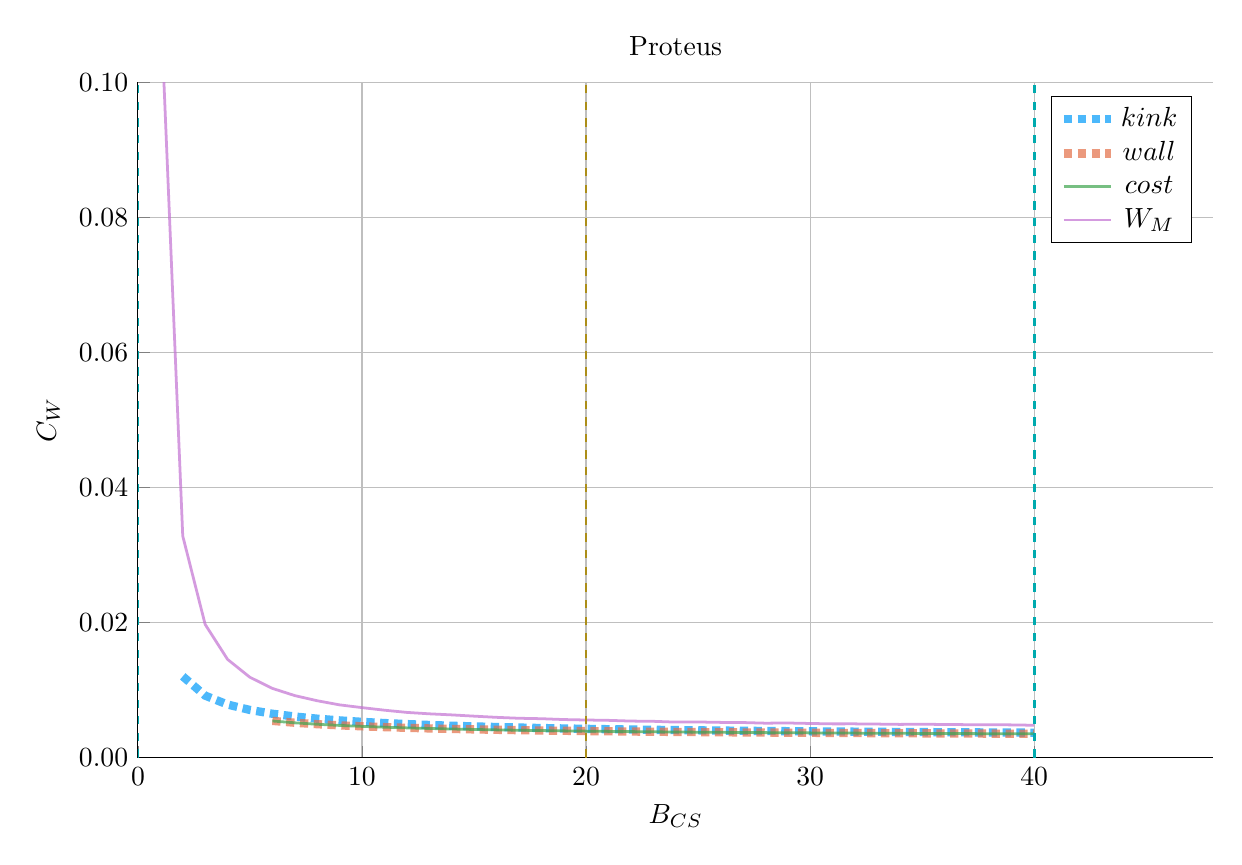
\begin{tikzpicture}[]
\begin{axis}[height = {101.6mm}, ylabel = {${C}_{W}$}, title = {Proteus}, xmin = {0.0}, xmax = {48.0}, ymax = {0.1}, xlabel = {${B}_{CS}$}, {unbounded coords=jump, scaled x ticks = false, xticklabel style={rotate = 0}, xmajorgrids = true, xtick = {0.0,10.0,20.0,30.0,40.0}, xticklabels = {0,10,20,30,40}, xtick align = inside, axis lines* = left, scaled y ticks = false, yticklabel style={rotate = 0}, ymajorgrids = true, ytick = {0.0,0.02,0.04,0.06,0.08,0.1}, yticklabels = {0.00,0.02,0.04,0.06,0.08,0.10}, ytick align = inside, axis lines* = left,     xshift = 0.0mm,
    yshift = 0.0mm,
    axis background/.style={fill={rgb,1:red,1.00000000;green,1.00000000;blue,1.00000000}}
, colorbar style={title=}}, ymin = {0.0}, width = {152.4mm}]\addplot+ [color = {rgb,1:red,0.00000000;green,0.60560316;blue,0.97868012},
draw opacity=0.7,
line width=3,
dotted,mark = none,
mark size = 2.0,
mark options = {
    color = {rgb,1:red,0.00000000;green,0.00000000;blue,0.00000000}, draw opacity = 0.7,
    fill = {rgb,1:red,0.00000000;green,0.60560316;blue,0.97868012}, fill opacity = 0.7,
    line width = 1,
    rotate = 0,
    solid
}]coordinates {
(2.0, 0.01203588028473762)
(3.0, 0.009184398565447248)
(4.0, 0.007862884013421416)
(5.0, 0.007057989599185806)
(6.0, 0.006502613319842857)
(7.0, 0.006090672614199328)
(8.0, 0.005770350019203115)
(9.0, 0.005512859892710094)
(10.0, 0.005300727695239639)
(11.0, 0.005122630604633569)
(12.0, 0.004970854616305319)
(13.0, 0.00483993073972795)
(14.0, 0.0047258536533321)
(15.0, 0.004625609812173743)
(16.0, 0.004536878856245803)
(17.0, 0.004457840030041975)
(18.0, 0.004387039347241793)
(19.0, 0.004323297793305687)
(20.0, 0.004265648725148842)
(21.0, 0.00421328852908289)
(22.0, 0.004165543387382086)
(23.0, 0.0041218418382133306)
(24.0, 0.004081697424729452)
(25.0, 0.004044691025187507)
(26.0, 0.004010460170934446)
(27.0, 0.00397868942182741)
(28.0, 0.003949102890414613)
(29.0, 0.003921458228696752)
(30.0, 0.0038955417483358588)
(31.0, 0.00387116442730114)
(32.0, 0.003848158715413871)
(33.0, 0.0038263753834889853)
(34.0, 0.003805681791784416)
(35.0, 0.0037859598267780737)
(36.0, 0.003767103936991627)
(37.0, 0.003749019788626583)
(38.0, 0.0037316235037579658)
(39.0, 0.0037148400629903496)
(40.0, 0.003698602652227772)
};
\addlegendentry{$kink$}
\addplot+ [color = {rgb,1:red,0.88887350;green,0.43564919;blue,0.27812294},
draw opacity=0.7,
line width=3,
dotted,mark = none,
mark size = 2.0,
mark options = {
    color = {rgb,1:red,0.00000000;green,0.00000000;blue,0.00000000}, draw opacity = 0.7,
    fill = {rgb,1:red,0.88887350;green,0.43564919;blue,0.27812294}, fill opacity = 0.7,
    line width = 1,
    rotate = 0,
    solid
}]coordinates {
(6.0, 0.0054444534313977866)
(7.0, 0.005168634641274746)
(8.0, 0.004954271193511655)
(9.0, 0.004781774855931542)
(10.0, 0.0046393940524333595)
(11.0, 0.004519572327657892)
(12.0, 0.004417187891782309)
(13.0, 0.004328621916738755)
(14.0, 0.004251229863078844)
(15.0, 0.004183024392188461)
(16.0, 0.004122476375660697)
(17.0, 0.004068385219748399)
(18.0, 0.004019791621043741)
(19.0, 0.003975917241919141)
(20.0, 0.003936121998618529)
(21.0, 0.0038998731854890116)
(22.0, 0.0038667227426346573)
(23.0, 0.0038362902440819057)
(24.0, 0.003808249979473852)
(25.0, 0.003782321013899768)
(26.0, 0.003758259446775421)
(27.0, 0.003735852316365348)
(28.0, 0.0037149127505960292)
(29.0, 0.0036952760721994664)
(30.0, 0.003676796641638663)
(31.0, 0.003659345275564596)
(32.0, 0.003642807117806076)
(33.0, 0.0036270798687725717)
(34.0, 0.003612072300608303)
(35.0, 0.0035977030015636596)
(36.0, 0.0035838993052924165)
(37.0, 0.003570596370170802)
(38.0, 0.0035577363809944163)
(39.0, 0.003545267851071995)
(40.0, 0.003533145007184075)
};
\addlegendentry{$wall$}
\addplot+ [color = {rgb,1:red,0.24222430;green,0.64327509;blue,0.30444865},
draw opacity=0.7,
line width=1,
solid,mark = none,
mark size = 2.0,
mark options = {
    color = {rgb,1:red,0.00000000;green,0.00000000;blue,0.00000000}, draw opacity = 0.7,
    fill = {rgb,1:red,0.24222430;green,0.64327509;blue,0.30444865}, fill opacity = 0.7,
    line width = 1,
    rotate = 0,
    solid
}]coordinates {
(6.0, 0.005431918985170686) 
(7.0, 0.005156651927896806)
(8.0, 0.0049427222925668)
(9.0, 0.004770577307210836)
(10.0, 0.004628487505103093)
(11.0, 0.004508911021409933)
(12.0, 0.004406736153465557)
(13.0, 0.004318351239259131)
(14.0, 0.0042411171388798095)
(15.0, 0.004173050519899446)
(16.0, 0.00411262543808849)
(17.0, 0.0040586437812760905)
(18.0, 0.004010148222137883)
(19.0, 0.003966362101140297)
(20.0, 0.003926646631736614)
(21.0, 0.003890470261769361)
(22.0, 0.003857385855340664)
(23.0, 0.003827013846123357)
(24.0, 0.003799029152446192)
(25.0, 0.0037731515135378028)
(26.0, 0.0037491374742800476)
(27.0, 0.003726774572373303)
(28.0, 0.0037058763309042774)
(29.0, 0.0036862784148944654)
(30.0, 0.0036678355176402353)
(31.0, 0.0036504187072176437)
(32.0, 0.0036339133609214515)
(33.0, 0.003618217419267161)
(34.0, 0.003603239855200063)
(35.0, 0.0035888993956205303)
(36.0, 0.003575123536625824)
(37.0, 0.0035618476053302967)
(38.0, 0.00354901385682175)
(39.0, 0.0035365709088021192)
(40.0, 0.0035244731223137145)
};
\addlegendentry{$cost$}
\addplot+ [color = {rgb,1:red,0.76444018;green,0.44411178;blue,0.82429754},
draw opacity=0.7,
line width=1,
solid,mark = none,
mark size = 2.0,
mark options = {
    color = {rgb,1:red,0.00000000;green,0.00000000;blue,0.00000000}, draw opacity = 0.7,
    fill = {rgb,1:red,0.76444018;green,0.44411178;blue,0.82429754}, fill opacity = 0.7,
    line width = 1,
    rotate = 0,
    solid
}]coordinates {
(1.0, 0.11281791824873516)
(2.0, 0.032817502153924004)
(3.0, 0.019728226993225767)
(4.0, 0.014550673387607675)
(5.0, 0.01189537503222638)
(6.0, 0.010254586386818185)
(7.0, 0.009187722848027494)
(8.0, 0.008426409595366063)
(9.0, 0.007814460956383539)
(10.0, 0.007407116893402244)
(11.0, 0.007026609234473925)
(12.0, 0.006699623094822548)
(13.0, 0.006490049586328449)
(14.0, 0.006332285776340749)
(15.0, 0.006145121123500574)
(16.0, 0.005968637732544897)
(17.0, 0.005831116183284295)
(18.0, 0.005766436928694199)
(19.0, 0.005641758652539625)
(20.0, 0.005573536740322697)
(21.0, 0.005522757977005573)
(22.0, 0.005416005772196298)
(23.0, 0.005379655600977924)
(24.0, 0.005261536268439173)
(25.0, 0.005281022329992938)
(26.0, 0.0052218684208626695)
(27.0, 0.005199327855049588)
(28.0, 0.005104248642193906)
(29.0, 0.005130959429711627)
(30.0, 0.005061392939220031)
(31.0, 0.005001395595923804)
(32.0, 0.005003038146366862)
(33.0, 0.004969709625977857)
(34.0, 0.004924506782614121)
(35.0, 0.004946663939864212)
(36.0, 0.004912455965902953)
(37.0, 0.004883749116586274)
(38.0, 0.004871307710986148)
(39.0, 0.004851151446945242)
(40.0, 0.004795575554984452)
};
\addlegendentry{$W_M$}
\addplot+ [color = {rgb,1:red,0.67554396;green,0.55566233;blue,0.09423434},
draw opacity=1.0,
line width=1,
dashed,mark = none,
mark size = 2.0,
mark options = {
    color = {rgb,1:red,0.00000000;green,0.00000000;blue,0.00000000}, draw opacity = 1.0,
    fill = {rgb,1:red,0.67554396;green,0.55566233;blue,0.09423434}, fill opacity = 1.0,
    line width = 1,
    rotate = 0,
    solid
},forget plot]coordinates {
(20.0, 0.0)
(20.0, 0.1)
};
\addplot+ [color = {rgb,1:red,0.00000048;green,0.66575898;blue,0.68099695},
draw opacity=1.0,
line width=1,
dashed,mark = none,
mark size = 2.0,
mark options = {
    color = {rgb,1:red,0.00000000;green,0.00000000;blue,0.00000000}, draw opacity = 1.0,
    fill = {rgb,1:red,0.00000048;green,0.66575898;blue,0.68099695}, fill opacity = 1.0,
    line width = 1,
    rotate = 0,
    solid
},forget plot]coordinates {
(0.0, 0.0)
(0.0, 0.1)
};
\addplot+ [color = {rgb,1:red,0.00000048;green,0.66575898;blue,0.68099695},
draw opacity=1.0,
line width=1,
dashed,mark = none,
mark size = 2.0,
mark options = {
    color = {rgb,1:red,0.00000000;green,0.00000000;blue,0.00000000}, draw opacity = 1.0,
    fill = {rgb,1:red,0.00000048;green,0.66575898;blue,0.68099695}, fill opacity = 1.0,
    line width = 1,
    rotate = 0,
    solid
},forget plot]coordinates {
(40.0, 0.0)
(40.0, 0.1)
};
\end{axis}

\end{tikzpicture}

    \end{adjustbox}
        \caption{Solenoid Strength Sensitivity}
    \end{subfigure}
    \hfill
    \begin{subfigure}[t]{0.48\textwidth}
        \centering
    \begin{adjustbox}{width=\textwidth}
      \Large
      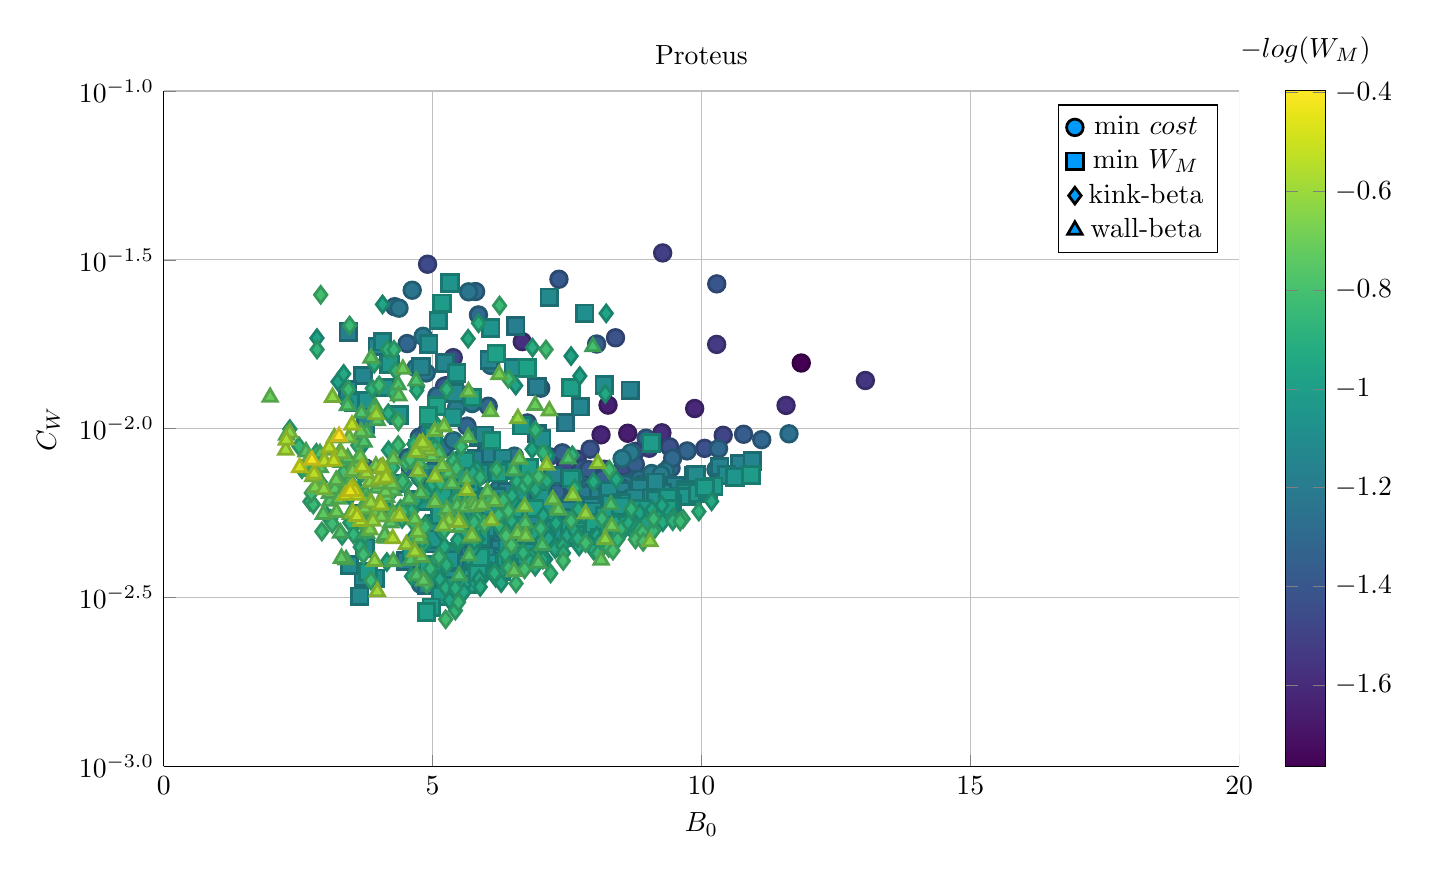
\begin{tikzpicture}[]
\begin{axis}[colorbar = {true}, height = {101.6mm}, ylabel = {${C}_{W}$}, title = {Proteus}, xmin = {0.0}, xmax = {20.0}, ymax = {0.1}, ymode = {log}, xlabel = {${B}_{0}$}, {unbounded coords=jump, scaled x ticks = false, xticklabel style={rotate = 0}, xmajorgrids = true, xtick = {0.0,5.0,10.0,15.0,20.0}, xticklabels = {0,5,10,15,20}, xtick align = inside, axis lines* = left, scaled y ticks = false, yticklabel style={rotate = 0}, log basis y=10, ymajorgrids = true, ytick = {0.001,0.0031622776601683794,0.01,0.03162277660168379,0.1}, yticklabels = {$10^{-3.0}$,$10^{-2.5}$,$10^{-2.0}$,$10^{-1.5}$,$10^{-1.0}$}, ytick align = inside, axis lines* = left,     xshift = 0.0mm,
    yshift = 0.0mm,
    axis background/.style={fill={rgb,1:red,1.00000000;green,1.00000000;blue,1.00000000}}
, colormap={plots}{rgb=(0.26700400,0.00487400,0.32941500), rgb=(0.27794100,0.05632400,0.38119100), rgb=(0.28291000,0.10539300,0.42690200), rgb=(0.28229000,0.14591200,0.46151000), rgb=(0.27619400,0.19007400,0.49300100), rgb=(0.26514500,0.23295600,0.51659900), rgb=(0.25042500,0.27429000,0.53310300), rgb=(0.23360300,0.31382800,0.54391400), rgb=(0.21813000,0.34743200,0.55003800), rgb=(0.20123900,0.38367000,0.55429400), rgb=(0.18555600,0.41857000,0.55675300), rgb=(0.17117600,0.45253000,0.55796500), rgb=(0.15772900,0.48593200,0.55801300), rgb=(0.14618000,0.51541300,0.55682300), rgb=(0.13374300,0.54853500,0.55354100), rgb=(0.12346300,0.58168700,0.54744500), rgb=(0.11948300,0.61481700,0.53769200), rgb=(0.12632600,0.64410700,0.52531100), rgb=(0.15014800,0.67663100,0.50658900), rgb=(0.19109000,0.70836600,0.48228400), rgb=(0.24607000,0.73891000,0.45202400), rgb=(0.31192500,0.76782200,0.41558600), rgb=(0.37777900,0.79178100,0.37793900), rgb=(0.45867400,0.81636300,0.32972700), rgb=(0.54552400,0.83803900,0.27562600), rgb=(0.63690200,0.85654200,0.21662000), rgb=(0.73088900,0.87191600,0.15602900), rgb=(0.81457600,0.88339300,0.11034700), rgb=(0.90631100,0.89485500,0.09812500), rgb=(0.99324800,0.90615700,0.14393600)}, colorbar style={title=$-log( W_M )$}}, ymin = {0.001}, width = {152.4mm}]\addplot+[scatter, scatter src=explicit, only marks = {true}, color = {rgb,1:red,0.00000000;green,0.60560316;blue,0.97868012},
draw opacity=1,
line width=0,
solid,mark = *,
mark size = 3.0,
mark options = {
    color = {rgb,1:red,0.00000000;green,0.00000000;blue,0.00000000}, draw opacity = 1.0,
    fill = {rgb,1:red,0.00000000;green,0.60560316;blue,0.97868012}, fill opacity = 1,
    line width = 1,
    rotate = 0,
    solid
}] coordinates {
(11.855851167264671, 0.015650867313707448) [-1.7651507846396934]
(8.62894306410229, 0.009694646552347688) [-1.652530796858066]
(8.262669569295957, 0.011744038729478485) [-1.647000146345283]
(8.132345586482765, 0.009590177278586947) [-1.6184546481250472]
(9.87352129314419, 0.011474300333025303) [-1.6124908438767973]
(9.26466071494926, 0.00972401084478665) [-1.5828949402967583]
(6.667811597046653, 0.018106858351787505) [-1.577618500437912]
(11.573395463568893, 0.011719738653164523) [-1.56873554690934]
(5.264528343635174, 0.013419897432724169) [-1.5599002750009094]
(13.048135395345042, 0.013892471464509717) [-1.5518482038436605]
(10.282796584070674, 0.017767343192357253) [-1.5302287668791192]
(9.278542294221232, 0.033146306422516245) [-1.5115301730224102]
(7.5044360623009565, 0.007510212646674021) [-1.5013825191439996]
(9.02784009554164, 0.008751202105526691) [-1.4958902811815062]
(8.710683108208965, 0.00816949735167802) [-1.4892617900728689]
(7.687377168804008, 0.008118078139228204) [-1.4884348201277007]
(10.404534949568816, 0.009559158760396884) [-1.4866425610729714]
(5.384524713145202, 0.01623184139531336) [-1.4835478223239928]
(7.472857057569771, 0.007837831837729894) [-1.4780728724015184]
(4.906484287411937, 0.03069401611625924) [-1.4650031348255397]
(7.111580297007043, 0.006765803188842749) [-1.4601242927308113]
(8.773685022223647, 0.008568870415676909) [-1.453691298071198]
(8.545510256202396, 0.007723927816166263) [-1.4489094778079963]
(7.070436548811644, 0.006162431971740805) [-1.432973868001932]
(6.884154096232421, 0.006329451983138475) [-1.4325147285303634]
(9.405921329983288, 0.008839617844718544) [-1.4268866569895065]
(10.057985274469397, 0.008744700190770928) [-1.4268347679685771]
(8.401821549997786, 0.018590297650719324) [-1.4237681445033143]
(8.189937032371649, 0.007587250291191641) [-1.4234658725845162]
(8.234578254729767, 0.007390656211515189) [-1.4109108269606008]
(7.92991212471289, 0.008694085637837138) [-1.4079262096010774]
(6.59839258184741, 0.00634066157530613) [-1.407330123320285]
(10.284931156770094, 0.026840973164111593) [-1.3996791570309395]
(7.3137838143058795, 0.007040053838733538) [-1.3974870797438]
(5.221820332167986, 0.013359280479800206) [-1.3946269662443698]
(7.785957307166937, 0.007634837530984513) [-1.3905305073664083]
(7.069469201177765, 0.006488653571629467) [-1.3895960301339119]
(6.200523563918331, 0.00554611680879456) [-1.381931002288656]
(7.340133149046422, 0.00695131625200887) [-1.3818272949203658]
(7.349866215424601, 0.027704627448181397) [-1.3812563757949996]
(7.351199097200025, 0.00681167564679013) [-1.379699079550137]
(8.120289345307025, 0.006715817539753603) [-1.376650573885692]
(7.90274300232169, 0.00757067906104037) [-1.3758581110553065]
(7.565484576443418, 0.006499559071472007) [-1.375220700855124]
(7.688718501611012, 0.00646934556613389) [-1.3742348635950123]
(7.005633077388933, 0.0063267927368600325) [-1.3713423550361032]
(7.166534585210968, 0.008267480512087599) [-1.370057699317172]
(5.695615872659735, 0.004988896324536347) [-1.3686239973313072]
(6.620180775083285, 0.005540386026064644) [-1.3680076928767484]
(5.712356159098289, 0.005024205798518008) [-1.3672266212882762]
(10.783439028923059, 0.009628839399324697) [-1.3667105305870977]
(6.000471468140266, 0.0050592629231849704) [-1.3651176317240314]
(8.050752136473724, 0.017814080806893125) [-1.3612722200713383]
(8.77043990632116, 0.007840171434328094) [-1.360737823431438]
(7.010340303297389, 0.013182987051350502) [-1.3596008789905631]
(7.295294539644262, 0.006730765435871485) [-1.3568098625263256]
(6.641599582701438, 0.005632641769207446) [-1.3562925407270994]
(6.645748730966029, 0.005613911931897123) [-1.3540300242042478]
(6.054699810485283, 0.005176189759381431) [-1.3527684291391184]
(9.401252816575663, 0.007678792615766904) [-1.3513432280511455]
(5.581708167132495, 0.006888425944911811) [-1.3508742741062625]
(7.803535098905909, 0.006674090356682625) [-1.348444904526092]
(6.76411548346407, 0.010402669872398145) [-1.3482429808137002]
(8.969455503638764, 0.009376571407375644) [-1.3481015746033576]
(5.634510628688515, 0.012583797530216616) [-1.34746159692277]
(8.156032796881272, 0.007115527316776566) [-1.3450418873098828]
(7.056939291922313, 0.006464286011476574) [-1.3449397649071608]
(7.240799475525162, 0.006186516144095541) [-1.344834769873685]
(6.571134452649435, 0.0053864817732829605) [-1.3436955024234147]
(7.4120702527384665, 0.00848434463520388) [-1.3426163725681677]
(5.934011898969639, 0.004938310227983135) [-1.3374912582230194]
(7.37766442956072, 0.006636608478826529) [-1.335539302100867]
(5.026669706190863, 0.007606581585076429) [-1.3352915983538123]
(6.825792187162438, 0.006029019944814239) [-1.331337874103357]
(9.732916904654346, 0.008594819258321628) [-1.3310780697195672]
(5.698038434377145, 0.004728216221281147) [-1.3292068036291638]
(6.854283769326888, 0.005953363383436291) [-1.32828646244698]
(4.7527705925878685, 0.009441137210103956) [-1.3280975618898123]
(6.452485475407575, 0.005079524630506098) [-1.3278697867431468]
(6.6282734062471, 0.005749625528658903) [-1.327757292865828]
(7.362442088263758, 0.006249734903697681) [-1.3253106415861637]
(6.357926345811093, 0.005155209960292018) [-1.3237407060184172]
(9.434691757978365, 0.007650804529712704) [-1.3217246458754282]
(5.945683748997239, 0.004926318213851794) [-1.319376268743699]
(5.716699212704698, 0.004774448071559269) [-1.3182101821558738]
(7.9999703999657505, 0.0066268624262571275) [-1.31770129332637]
(4.526018058829261, 0.017867829271260238) [-1.3171626271127284]
(7.307142270921693, 0.006479743346210051) [-1.3144438328362922]
(5.64022055353738, 0.010177994071422254) [-1.314397397461996]
(11.121291715489328, 0.009279261565995508) [-1.3134452963620502]
(6.890660641840135, 0.005896178522672516) [-1.3126768401499638]
(5.8496112618323926, 0.007223214696135702) [-1.3123916957087167]
(3.755618871416242, 0.007643344629724278) [-1.3117090270675453]
(6.965828665871357, 0.0062843154751196315) [-1.3112976001573549]
(7.132942553696917, 0.006316305209750007) [-1.3102933400586538]
(6.034623082086722, 0.011655743235665423) [-1.3084666426112759]
(9.464190150712176, 0.008181643780093392) [-1.3081739820914746]
(6.735484315816856, 0.005920113041607297) [-1.3081169022767745]
(6.329532230716051, 0.005266304291939928) [-1.3075986397555424]
(6.949512174456946, 0.0056632699287416785) [-1.3038897119548887]
(5.7123865302563095, 0.004515583648974614) [-1.3034916079905217]
(4.588431546307119, 0.00762405310841983) [-1.301506470226052]
(5.8529754306366, 0.021723513711501174) [-1.2978787946122285]
(6.763583440942078, 0.005860560202229156) [-1.297460949292816]
(5.79974352272628, 0.02547444831481485) [-1.2953226778576867]
(4.294506467374343, 0.022974551007964673) [-1.2951062787178942]
(10.317711969577175, 0.008727794605170999) [-1.2946978796261759]
(7.030442720189729, 0.00606442154900928) [-1.293243062455323]
(6.3155245633398005, 0.00478216163852665) [-1.2916316854649297]
(5.594153930448576, 0.004505685536187866) [-1.291573412415986]
(7.0608047385200905, 0.006201757851874389) [-1.2910367642815292]
(8.746159160738731, 0.007056272547770033) [-1.2894268757747884]
(5.790961836119614, 0.004812007322004063) [-1.2891780169645117]
(7.13931972393237, 0.005900795309436559) [-1.2883016772579983]
(5.642350264315365, 0.004575860387174974) [-1.2877120777365891]
(5.500511487756749, 0.007501625869556503) [-1.2825608117529994]
(5.1870060839860015, 0.004048206616482656) [-1.2803416949249293]
(5.0793762257146975, 0.012501014524680899) [-1.2790944723531177]
(4.900710067477188, 0.009849033693022476) [-1.2789599032268324]
(5.416336002756713, 0.004266328381972482) [-1.278637308935949]
(7.047880217226236, 0.00602317781329061) [-1.2752962713941192]
(4.537987048593646, 0.008202673797589401) [-1.2724318730764337]
(6.7947527911354095, 0.005313590913225172) [-1.26778944603233]
(7.547856502776895, 0.005746237915345085) [-1.2652894696394015]
(8.337373800803634, 0.0063394092295352205) [-1.263844406219344]
(5.839234828237175, 0.004670640784960837) [-1.2622412045786418]
(6.307588148065544, 0.005025369604276285) [-1.2622057750392766]
(6.369182324037021, 0.004715175023029078) [-1.2568407944078956]
(7.25221896281004, 0.005515822538041083) [-1.2564369672634057]
(5.207422458409709, 0.008763742702873716) [-1.255580803936347]
(8.846964102011665, 0.007090160917314494) [-1.2542825781236586]
(11.62801313878366, 0.009658252430988482) [-1.253606675738751]
(6.586437041421525, 0.005078101074449218) [-1.2533258835374417]
(5.896819232149536, 0.004668333949768413) [-1.252740293490489]
(7.218625057420257, 0.005623439530060779) [-1.2512906609771755]
(4.770007649977626, 0.007192663750971734) [-1.2505906665339703]
(6.391248250395476, 0.004753912504004936) [-1.2505667349102745]
(6.722228809625436, 0.00547669175115548) [-1.2505409706978425]
(5.9975644347104575, 0.008585550973626429) [-1.2504311283223648]
(6.220483255591395, 0.00536142422310656) [-1.2495193060816674]
(7.131398255569569, 0.005891517799670805) [-1.2472203996667584]
(4.620896334693883, 0.025703839631456088) [-1.246340221801285]
(5.634708074324937, 0.004426672964739238) [-1.246337044553182]
(6.0053836269885, 0.004733745531528537) [-1.2444533586241864]
(6.122472771064873, 0.004373459187272198) [-1.2410504069560844]
(4.881468969197191, 0.014622918962551527) [-1.2404616678069278]
(5.669873863181108, 0.025422666134658947) [-1.2402101811954278]
(9.159921449108527, 0.00699405114862055) [-1.2399625556579728]
(6.619988989498716, 0.005459593535350185) [-1.2395775558220574]
(4.0721743569002395, 0.006780135026174841) [-1.238968027160994]
(8.487125648729805, 0.006381273355008305) [-1.2381935518916032]
(5.785136288326493, 0.005454977773134567) [-1.2372164242860222]
(7.805870043590986, 0.006162937475975255) [-1.2359322527835273]
(6.521775930847536, 0.008295248979234676) [-1.2345953253761524]
(7.299795216034374, 0.005661235915534237) [-1.2333782101635051]
(6.654376116038794, 0.005116145429327062) [-1.2329256482335589]
(8.586321868785943, 0.0068738253515159406) [-1.2318041138227]
(5.871716076416853, 0.007759607253139788) [-1.2286780396839752]
(5.525881431830733, 0.004270512991179436) [-1.225800447150557]
(4.37566370657649, 0.022744869820021597) [-1.2237626122718148]
(5.386416012885563, 0.009221148903357415) [-1.2192315569877235]
(5.735606858683557, 0.011868028475244749) [-1.2191811590789894]
(8.68706974133124, 0.008481483201532794) [-1.2185680785343938]
(8.63032181590475, 0.00622802822970762) [-1.2179132583990178]
(8.508158073563377, 0.006703260233628488) [-1.2171472173843672]
(7.953691408978824, 0.00633213628058925) [-1.2167448502658762]
(6.081331959057098, 0.015392818825938645) [-1.2162995250149307]
(5.225401290559421, 0.003872910530196867) [-1.215703789534109]
(5.988978974443945, 0.004720977485089404) [-1.2156312790675603]
(9.073087462786646, 0.00736963569440644) [-1.2145283350978044]
(7.217725198328268, 0.005383150867826381) [-1.214317974252912]
(5.536577745729214, 0.004178935326843822) [-1.2138536176262873]
(4.776559777248383, 0.0034641548226198885) [-1.2119360055173332]
(5.211688187540344, 0.0038140534914709043) [-1.2104347246988538]
(10.269380266980404, 0.007570292211977012) [-1.2084631186053005]
(6.918845939903695, 0.0052385995930077645) [-1.2083264519217767]
(7.0692693982238906, 0.005083028024589718) [-1.2073346872626274]
(5.874112036399968, 0.004039129704078142) [-1.2071975929322125]
(4.690082401892927, 0.01513911751066285) [-1.2067840670536927]
(7.861161945792819, 0.006395373245847939) [-1.206736577191552]
(9.326423266814658, 0.007483645463069493) [-1.2065799786199445]
(8.029413669351802, 0.005698374888186277) [-1.203843641047789]
(6.959732144718079, 0.005550896360654382) [-1.203724365314369]
(6.960477287319412, 0.005010777712400389) [-1.2024406864855146]
(7.654476699386534, 0.007157947201399507) [-1.2021169810907544]
(4.823547237227045, 0.01877759730610099) [-1.2015933815507112]
(6.062862639710857, 0.004489267037355289) [-1.2014423796656961]
(8.999102001729389, 0.006374667856956503) [-1.2011965112492808]
(7.2717504340335415, 0.00572395742880883) [-1.2005427289121806]
(6.227413325881237, 0.0066192080125215165) [-1.1994215784439877]
(9.247503176233229, 0.007316062816603203) [-1.1975084180232178]
(5.443249511926066, 0.011502671870448664) [-1.1972619972446426]
(6.742357647461489, 0.005266662336518346) [-1.1967371969067386]
(5.926964832086266, 0.004368135902166705) [-1.1965134818457024]
(8.524769827029726, 0.008154332104698897) [-1.196084536648355]
(8.867575034400405, 0.006843978332329513) [-1.1943424204563022]
(6.457339766119646, 0.005029914775543452) [-1.1908054127888088]
};
\addlegendentry{min $cost$}
\addlegendentry{min $W_M$}
\addlegendentry{kink-beta}
\addlegendentry{wall-beta}
\addplot+[scatter, scatter src=explicit, only marks = {true}, color = {rgb,1:red,0.00000000;green,0.60560316;blue,0.97868012},
draw opacity=1,
line width=0,
solid,mark = square*,
mark size = 3.0,
mark options = {
    color = {rgb,1:red,0.00000000;green,0.00000000;blue,0.00000000}, draw opacity = 1.0,
    fill = {rgb,1:red,0.00000000;green,0.60560316;blue,0.97868012}, fill opacity = 1,
    line width = 1,
    rotate = 0,
    solid
}] coordinates {
(7.4724590738720655, 0.010422279639263054) [-1.1890033537880158]
(6.938996985119089, 0.009658294464102987) [-1.1883675827161198]
(6.9393893920794385, 0.013313745665171912) [-1.1879538738656286]
(6.377850385556073, 0.006487414571263668) [-1.1878029685724296]
(6.547487324963764, 0.020145877705477357) [-1.186260879134981]
(8.029613686159495, 0.005801884747670386) [-1.1859242026174677]
(5.6874025972941205, 0.004217349677698315) [-1.183889066210908]
(7.827309596895398, 0.0058827996938258294) [-1.1830291222504283]
(5.8219713598117036, 0.008160599297710009) [-1.1826268505607591]
(6.946718058585209, 0.004857174007518612) [-1.182365307189366]
(3.434094114791118, 0.01935279381255584) [-1.1822251925764147]
(6.23809783755075, 0.00447855648592392) [-1.1813612663460882]
(5.88781791976068, 0.00428725320402622) [-1.1785285195809967]
(4.505121226933233, 0.004053651772674214) [-1.1775655951090325]
(6.553162158329651, 0.005121496915389368) [-1.17705398157876]
(5.8303432949169745, 0.005890819973806921) [-1.1767452937515073]
(8.807822926389145, 0.006104718148251412) [-1.1766083315756861]
(4.18691738643155, 0.01556268699280997) [-1.173888237216638]
(7.55203601905607, 0.005882961839613334) [-1.1734465174435744]
(5.819836385827624, 0.005961179911412564) [-1.1729466514857931]
(9.116693027577789, 0.006287276174883399) [-1.172839252676928]
(3.659189590525744, 0.005599267038542826) [-1.1727769211527406]
(7.004035835152084, 0.005070632392189801) [-1.1727372361954858]
(4.897086463141796, 0.003434292526080427) [-1.1726542785062386]
(8.087708955601924, 0.0062657093568900535) [-1.1703764252048678]
(6.7024429891400565, 0.004942047034638912) [-1.1699166462753263]
(5.893015258208656, 0.004183590560340062) [-1.1681831393061217]
(7.479710666339309, 0.005170881199231806) [-1.1671080842733117]
(9.508375514310952, 0.006777996547666784) [-1.1655606692177785]
(6.075560203652315, 0.008402469668507205) [-1.165303541813206]
(6.61932998550545, 0.004666935296152095) [-1.1643973078802388]
(6.286558265163782, 0.004663766235492665) [-1.1632535008384055]
(5.050068824721165, 0.004566940606242733) [-1.1631989573193973]
(7.688714523679582, 0.0054331000812183365) [-1.1630392685982025]
(8.505800422917172, 0.006544368204474158) [-1.1625753891662707]
(8.975209897762664, 0.006511116933487475) [-1.1617936783337066]
(8.380983437312786, 0.006126048639979384) [-1.159367616011031]
(8.67470730810651, 0.012995381528200805) [-1.1593260324319568]
(5.960621269295445, 0.004013416769217783) [-1.1592024857112633]
(6.282535161243701, 0.004530529794416821) [-1.1590403977294572]
(10.712436821713085, 0.007867971330715704) [-1.1589428109110296]
(7.099415207654768, 0.005330271588661515) [-1.158451320077056]
(10.3395352744249, 0.007724720119696045) [-1.157468772898154]
(6.536306152444655, 0.004436262085616985) [-1.1570637161067505]
(9.855000808062698, 0.007249642226094706) [-1.1563966451418943]
(5.856384724795581, 0.009420901412013665) [-1.1561531921827275]
(7.454679880823048, 0.0057898611640113395) [-1.1538328200442942]
(5.14753239685863, 0.007237376261288284) [-1.1525173430901554]
(6.856563325018079, 0.004881019954742076) [-1.1522162283529644]
(7.618840457764884, 0.0059379940430840635) [-1.151968932860403]
(8.398440991699191, 0.0061407721476487214) [-1.1511586507355254]
(4.781165601129724, 0.015255960449664327) [-1.1509834966159156]
(6.247011281135245, 0.004419080970160178) [-1.1503660387736743]
(3.7553680100049234, 0.01032617135589161) [-1.1500086948877408]
(5.5152996897670015, 0.004014883666259908) [-1.1494080253790357]
(7.800728278542519, 0.005291422749753008) [-1.1493093072503229]
(6.054088477025007, 0.01598351560152435) [-1.1489823622220707]
(5.411295562966824, 0.003915099463846501) [-1.1484511044037433]
(7.052045109627868, 0.005020529922825154) [-1.1483999797493492]
(5.28488049549897, 0.0034947010100993764) [-1.147064765638366]
(7.62011089503286, 0.005859550653426385) [-1.1465028274549764]
(7.468210164743146, 0.005641165149475234) [-1.144883586902141]
(5.595946792423691, 0.007176119328254024) [-1.144368544047569]
(10.943656185786155, 0.00802165691682325) [-1.1435280806157744]
(7.908061023064291, 0.005447269817044685) [-1.1433393449411435]
(8.854582349908517, 0.006668732693209443) [-1.143332108158641]
(6.549837080949351, 0.004886014774808058) [-1.143184585873657]
(3.9729755898485215, 0.017515494611674454) [-1.1428249654095861]
(3.703954177548893, 0.014377117697389604) [-1.1427984862828113]
(3.4213090828497417, 0.013005276311642224) [-1.142397010267489]
(6.02709699747974, 0.005929095379259443) [-1.1423708774410877]
(5.231750077921478, 0.01565086593371781) [-1.1422424769576425]
(7.2349136535832095, 0.007266091038483963) [-1.140012696356206]
(7.647205004097057, 0.005840600330748377) [-1.1399465227440013]
(6.532016233135844, 0.00480284773560221) [-1.1387943392990294]
(7.523885505796154, 0.005752426766742318) [-1.1382802201938975]
(7.750130276532692, 0.011612930840038163) [-1.1380314198362265]
(9.276469763067444, 0.006446360072583165) [-1.137892443914052]
(5.952941013085345, 0.009562541252399106) [-1.1311113631375915]
(7.951426521304668, 0.005743536904522906) [-1.1302954325651586]
(5.952653119927932, 0.0041760314888273755) [-1.1295543261638465]
(8.253192497448524, 0.006161648966500728) [-1.129462828049983]
(5.512192429439468, 0.00369116854025651) [-1.1277963061708562]
(6.180741676638315, 0.006278926396423389) [-1.126807171194116]
(6.608627477861355, 0.004487529275565533) [-1.1267021554022474]
(9.14457555501132, 0.006938744439971839) [-1.1265761162904897]
(5.310301950330671, 0.004304336836767321) [-1.1261385034152473]
(7.969320198807478, 0.005917258047258142) [-1.1260458936236624]
(7.954215183655014, 0.005885263457738176) [-1.1250537668582923]
(6.771595293849517, 0.005616858230043609) [-1.124511019242948]
(6.641944516873176, 0.004843731890681865) [-1.1236988869720232]
(6.896134858333351, 0.005173923137495115) [-1.1235064786985465]
(3.7132325707792995, 0.003624821435760545) [-1.1232730371267585]
(4.936839162331792, 0.007429853985811719) [-1.1231293548483412]
(6.555316024199809, 0.005231942783984398) [-1.1209978185544383]
(6.304604592673814, 0.008169617815892689) [-1.1196911148335087]
(8.737416781995437, 0.0061580609115664325) [-1.1194748634113345]
(6.123815672401932, 0.004188882178419093) [-1.119418152841014]
(8.324353852438948, 0.005791769416647159) [-1.1191123923650526]
(6.830685941792606, 0.004931972266091366) [-1.1181736482095217]
(8.279157421008941, 0.005611347227289511) [-1.1176702646643628]
(7.172394160745635, 0.024480989089009208) [-1.1175403888423328]
(6.753756430979739, 0.004518885765871233) [-1.1174827013795072]
(8.76524294869496, 0.0062233325455323925) [-1.1174414411464733]
(5.952289891041446, 0.006299808378708293) [-1.1171134960728113]
(6.523754565443294, 0.004568184715721437) [-1.1171111976535804]
(5.4096290381473375, 0.012757776435747556) [-1.1168806186241906]
(9.896916686410892, 0.007305420869085463) [-1.1160945644374545]
(8.286804128590813, 0.005340773800773009) [-1.1139896885893594]
(5.399012890266871, 0.0036233885329560954) [-1.1123768792739945]
(8.296167355721272, 0.005311493039288053) [-1.1112153482766423]
(6.778775360762903, 0.0045000578497955725) [-1.1111283014916062]
(3.642453456441478, 0.003188662256079057) [-1.1108869662710774]
(6.918579935305505, 0.004842654136629077) [-1.1089922492653659]
(6.5071710234613676, 0.00452032863173795) [-1.108391782497311]
(7.258592477367294, 0.00535669926333167) [-1.1082929384878708]
(6.6776055936353265, 0.004745534590751309) [-1.1074346113685616]
(5.3226296796509205, 0.004323464728471098) [-1.1074227437950106]
(10.46985584146923, 0.007293078759243216) [-1.1069130893453907]
(3.4547855533452156, 0.003945456212149148) [-1.106325178133445]
(7.57975455174028, 0.004982808461571556) [-1.1060035644106432]
(5.06842585608741, 0.0052409052861536465) [-1.1038776732161713]
(5.698043204630489, 0.0065314531396132094) [-1.10351060592976]
(7.734654274692709, 0.005173060010686301) [-1.1022315889718237]
(6.228402773452205, 0.005951424789746293) [-1.1016702257969113]
(5.288893434740895, 0.007437806150470808) [-1.100448826904311]
(7.254453932047169, 0.005288339533793414) [-1.0998565094908217]
(6.807046489565401, 0.004337170224988449) [-1.0995498480529582]
(8.496667761878552, 0.005750254423520601) [-1.0992970719713648]
(6.506723144546308, 0.004423364554484401) [-1.0987351440216522]
(8.273277101596172, 0.006535275113176343) [-1.0983869460625248]
(7.024499917691516, 0.006822630998366228) [-1.0977261444257258]
(4.929559505548113, 0.017828562633364364) [-1.0969882385788774]
(6.546519891753608, 0.004407786879742766) [-1.096807077081938]
(6.299458688060015, 0.0041501216036249275) [-1.0962033310727437]
(5.917588131126826, 0.003972749736578854) [-1.0948458082881816]
(6.5027787367036485, 0.015155543307471772) [-1.093965318294314]
(8.191093731826841, 0.013471957430229371) [-1.093275686079877]
(5.765417917352738, 0.003923510470624812) [-1.0931318196649105]
(4.067683728143941, 0.01811006730780237) [-1.0926393639694263]
(5.643295069658257, 0.005671433069083637) [-1.09199330517098]
(5.33448260992027, 0.0035546432563184145) [-1.0916603258728452]
(5.996010919360583, 0.005082501155756355) [-1.091508438458307]
(6.130249778803564, 0.003922207642532424) [-1.0911853630489914]
(5.152309500808404, 0.007129588907950501) [-1.0896526200520398]
(6.613976143688219, 0.004468466025444819) [-1.088663441639713]
(7.828710312153846, 0.021949864805969728) [-1.0877780715734315]
(7.029871400370792, 0.009322832924906896) [-1.0870739196827126]
(6.6598420793586, 0.004672088916974179) [-1.0855818982110972]
(6.33097870945106, 0.004039319528471343) [-1.0844715994400023]
(7.702268833143657, 0.0053439960085053) [-1.0842780595786392]
(6.084754710909704, 0.005760793758021615) [-1.084266572782003]
(7.98999393987453, 0.00569380985136289) [-1.0839928767281124]
(5.068992476376386, 0.0039349920083461085) [-1.0828594792618813]
(9.086048642306793, 0.0062405207423892875) [-1.082853352734588]
(7.44906676523106, 0.0054577800846403015) [-1.0824719035597]
(5.375575122544495, 0.0035809652689903063) [-1.0824709528228211]
(7.386984140765724, 0.005148297391297789) [-1.0814366033908964]
(9.702271536107535, 0.006582162000449632) [-1.0809878234039578]
(9.614854186704672, 0.006301853688415234) [-1.0808972954130593]
(4.645688111866446, 0.006161790226168522) [-1.0797863646031054]
(3.927334262139488, 0.0036086053477567665) [-1.079163153355685]
(6.963971610592974, 0.004793357206410555) [-1.0780309855478056]
(8.244956752748422, 0.0054298508521766365) [-1.076806285491668]
(5.769697532800943, 0.00604411217248383) [-1.0765985094568509]
(7.283344319549832, 0.004828662165485411) [-1.0760641298404754]
(5.392578394594405, 0.005661819547798889) [-1.0757730303287785]
(3.7434225317786316, 0.00443044659495794) [-1.0744056068515366]
(7.7252366425534715, 0.005467468655559742) [-1.073726482715373]
(8.506016241294386, 0.006046667097602973) [-1.072815333291583]
(5.722077224788854, 0.006315687038558954) [-1.0718638391063322]
(3.5290681872248832, 0.011989877345034696) [-1.0710072465261937]
(5.408389828424612, 0.006287200186056995) [-1.0706716976099708]
(5.880603880610476, 0.00739594343637032) [-1.069478881808043]
(3.770984054785403, 0.012080600310741674) [-1.0679830462657767]
(9.144669371614333, 0.006138341400017388) [-1.0670572282884458]
(5.3325423351198395, 0.004085658341340117) [-1.0667391835901658]
(8.316799187366927, 0.006004004929014098) [-1.066302608545655]
(6.389619437625667, 0.004440975162005993) [-1.064104157833971]
(5.324355765249537, 0.026972932068461592) [-1.0640878812065675]
(6.511622532652898, 0.004395996587917252) [-1.0635820925869255]
(6.911249511094287, 0.004423420241739423) [-1.062988318250961]
(7.502962627592097, 0.00480727122317776) [-1.0628036997189863]
(5.469724443246719, 0.0034131330547271113) [-1.062700357913494]
(5.706475165604361, 0.0036974585830479817) [-1.0626514373993834]
(7.276669037534987, 0.004776499853086686) [-1.0610739421064752]
(6.526975357350624, 0.004144297606935685) [-1.0588352037418618]
(5.105089902831069, 0.0209014980088616) [-1.0585986545827941]
(4.374531653432859, 0.010988948677442597) [-1.057135771526312]
(4.122473679442906, 0.013241941603829825) [-1.056315661795303]
(6.078673477412938, 0.019862106250452566) [-1.0562734967702754]
(7.427558910001991, 0.004858658731965693) [-1.0561257856094448]
(7.01015270925273, 0.006223828461257365) [-1.0559814704124602]
(5.014809023336614, 0.004706089102701761) [-1.0555859489072712]
(6.029077134394886, 0.003994614402213268) [-1.0549803415205259]
(9.718000396033032, 0.006463993798881436) [-1.0545713902023608]
(5.896086527792721, 0.0038990516235787613) [-1.054205756099488]
(10.62632239203378, 0.007195479612398366) [-1.0536290024409787]
(9.830251746280974, 0.006286763322784177) [-1.0533216125601341]
(5.653429182632709, 0.004822724612666477) [-1.0529307720930816]
(7.148582094551358, 0.005656264568736301) [-1.0525850668019536]
(9.721783343528084, 0.006295530789348686) [-1.052552508886994]
(6.4747129291886205, 0.007550888758433211) [-1.0509835312174363]
(7.5553171987129115, 0.004904482654727138) [-1.0508250621973283]
(5.689433662550519, 0.006571304536184572) [-1.050680345054969]
(6.819358408267933, 0.004560195418506711) [-1.0506245233592775]
(5.372500908480495, 0.01080264515897382) [-1.0505217359121972]
(9.464104357867244, 0.00597835329976134) [-1.049317623712287]
(9.421645636318559, 0.00605275476812188) [-1.0490747591885061]
(6.83923495211403, 0.004511808104116367) [-1.0489907539423449]
(7.595014509377157, 0.0049153150140211965) [-1.0478434867034416]
(6.9492853284169565, 0.004616652674773231) [-1.0473758850488442]
(6.631954997333512, 0.006447737760929581) [-1.046767629611379]
(4.836574702453568, 0.006114416229637186) [-1.0460742739305466]
(5.447392742867525, 0.01461141466329314) [-1.0428746875530057]
(5.278008805745069, 0.0034297894059699906) [-1.0409932776852704]
(6.869290933859089, 0.004324846597058025) [-1.040720375777512]
(4.388359570069462, 0.0068957525832947) [-1.0400494553390642]
(7.730136216039545, 0.0047742837106654985) [-1.03963800286999]
(5.097390647393597, 0.0070972253563865) [-1.0394862991533038]
(5.705197239891871, 0.006107051538135721) [-1.0391370640013136]
(4.211114439903267, 0.015503036624972183) [-1.038354289214968]
(9.925180494788561, 0.006445735380428859) [-1.0380750082543837]
(8.392824243874195, 0.005205902574339689) [-1.0370263081612092]
(7.973811270774484, 0.005283195240312258) [-1.0365321066837632]
(8.49921904371083, 0.005892181423629392) [-1.0364145571368009]
(6.655649338522086, 0.010214094301379546) [-1.0358730287795153]
(6.272206414918943, 0.003781581128188247) [-1.0352797650690977]
(9.40142074331525, 0.0061316127141858145) [-1.0352425491421158]
(4.6061758509773245, 0.004345014451914255) [-1.0335536367675167]
(5.764426452876033, 0.00415632052734694) [-1.0319535365225938]
(9.372888478292797, 0.006253917955260214) [-1.031638330454266]
(5.729013310777877, 0.003613822408322808) [-1.0316283345953763]
(5.883030813164119, 0.00478160347928963) [-1.0312630056422283]
(6.556479558238363, 0.004326998549376461) [-1.030801418278412]
(6.395724956994062, 0.006039359373565179) [-1.0301227610636083]
(5.139256557257989, 0.005550817437725965) [-1.029015666765989]
(10.123332193763748, 0.006583295742064639) [-1.0288573869793878]
(6.568561456688728, 0.004204292638824563) [-1.0245024368116802]
(5.6039086370880105, 0.007145400138218064) [-1.0231385619546913]
(7.648719554707365, 0.004789677204757558) [-1.021449027000752]
(10.226601060349507, 0.00675373673736514) [-1.0213127693885564]
(5.153470412653239, 0.003193542226257652) [-1.0209276741398987]
(7.579001576207003, 0.007121099635585821) [-1.0202684704954939]
(3.8015765702844804, 0.0037708668397859442) [-1.0187837906200732]
(8.894908266877893, 0.005805595496214904) [-1.0179738483919518]
(9.066566182501706, 0.009070154520460257) [-1.0169425110693646]
(8.213444606213486, 0.00501503870041615) [-1.0162045101447212]
(10.062564168396998, 0.00670010251636303) [-1.0149810946438107]
(4.727731778507776, 0.008752580219573484) [-1.014353466976016]
(5.174769297851055, 0.023528952793841592) [-1.0140528730661398]
(8.195915051921629, 0.005527004085356763) [-1.0133093427968076]
(7.054369905297556, 0.004778958682375364) [-1.0128360857902137]
(5.031848935370691, 0.003842216867194081) [-1.0126834015105255]
(10.922140692684003, 0.007300503854095673) [-1.0124869131348806]
(5.915584448350069, 0.0038089628255598917) [-1.0084966915198963]
(5.602678326023923, 0.008048423371546378) [-1.005776006726422]
(7.544600594243294, 0.005136336479510988) [-1.0027757315503723]
(4.977942341177753, 0.0029594317443149176) [-1.002422823826331]
(5.642218938318191, 0.003459304695059543) [-1.0023352556688647]
(8.295019648678474, 0.004988217345842403) [-0.9994656987080655]
(7.070940189155582, 0.004649343635980374) [-0.9991953302395459]
(6.226711465325763, 0.007411548557741582) [-0.9991876183275935]
(6.419292049664728, 0.0038831217844692545) [-0.9971256954762724]
(4.887255844769486, 0.0028654321699102935) [-0.9968293366364798]
(7.7523402111694955, 0.004992975570566671) [-0.9965130838642419]
(5.890289877584987, 0.003830578946172306) [-0.9960911988132904]
(7.574296219984337, 0.013215773066776348) [-0.9953080727443692]
(9.012153601445592, 0.005338097758519931) [-0.994764309342816]
(9.386356586964215, 0.005798704578553127) [-0.9941918143808477]
(6.789856926677994, 0.007661762309327555) [-0.9939974184414383]
(5.741492166499531, 0.012372283627325148) [-0.9936895922796631]
(8.093840230774958, 0.0047417231470052315) [-0.9920762514365737]
(8.423301149042322, 0.005175409039233765) [-0.9891335090238219]
(6.5096125388500665, 0.005799134035216279) [-0.988320863141931]
(6.362065295698958, 0.003975692742134705) [-0.9873980470532571]
(6.898795759334327, 0.005803966541873779) [-0.9872638091155089]
(5.86662772167221, 0.005281651647264406) [-0.9871243344745786]
(5.00980677003057, 0.00954881671016918) [-0.9862026242600886]
(6.0980328290063905, 0.009231911938640338) [-0.9851939256634008]
(8.004532839270633, 0.005233428706224578) [-0.9845137991026185]
(6.760939557779194, 0.015110407509335635) [-0.9844063088607684]
(5.192252043701997, 0.006274740712107015) [-0.9843851675543582]
(6.182612803400956, 0.01666579340898781) [-0.9832677624207663]
(8.112468976523042, 0.004743145828135927) [-0.9823156156623659]
(5.841361480008224, 0.003744148435661381) [-0.9817957805945331]
(7.647006952351862, 0.0048552692105239565) [-0.9817262777133879]
(5.077285700891451, 0.01167873981501713) [-0.980944500204026]
(5.883453787587344, 0.004161496814710868) [-0.9808435285359967]
(4.920420200443467, 0.010903168023481107) [-0.9803069086017846]
(8.471906861597214, 0.005187973951951495) [-0.979926239566149]
(4.915731269106913, 0.0039527765780552285) [-0.9799255860420428]
};
\addlegendentry{min $cost$}
\addlegendentry{min $W_M$}
\addlegendentry{kink-beta}
\addlegendentry{wall-beta}
\addplot+[scatter, scatter src=explicit, only marks = {true}, color = {rgb,1:red,0.00000000;green,0.60560316;blue,0.97868012},
draw opacity=1,
line width=0,
solid,mark = diamond*,
mark size = 3.0,
mark options = {
    color = {rgb,1:red,0.00000000;green,0.00000000;blue,0.00000000}, draw opacity = 1.0,
    fill = {rgb,1:red,0.00000000;green,0.60560316;blue,0.97868012}, fill opacity = 1,
    line width = 1,
    rotate = 0,
    solid
}] coordinates {
(5.163569333804058, 0.0049343734079309275) [-0.9797193514246809]
(7.7377435890937285, 0.014326928101993836) [-0.9793649258547107]
(5.770648171127724, 0.004418560150536774) [-0.9793554194238832]
(4.7261265073999565, 0.007133046942930264) [-0.9793399260652301]
(4.749925847834237, 0.004527202123528333) [-0.9786718824413932]
(3.240965863210715, 0.013777079521683793) [-0.9784247640598123]
(8.408728218761828, 0.005278344797288595) [-0.9784156054323705]
(5.20936895107677, 0.004002965553163199) [-0.9772101816150688]
(6.546367069245276, 0.013418113026562503) [-0.9771245449599791]
(6.406431686907994, 0.004027289040267911) [-0.9768013676267739]
(2.8493674862886933, 0.018551171796247393) [-0.9763993914483391]
(4.701597365840406, 0.006130885121857039) [-0.9762949474128021]
(9.199948291326558, 0.005562603331167774) [-0.9759999361809304]
(7.151824598817379, 0.008328856003390762) [-0.9748577786630778]
(7.102409218167167, 0.004109700372311695) [-0.9738966318394574]
(8.195112351068081, 0.004913914166672265) [-0.9734793512186626]
(8.019705338927611, 0.004665122126804512) [-0.9731032751395803]
(4.288110261014516, 0.006640697404806304) [-0.9726016535105552]
(7.158134609952364, 0.004736078134325021) [-0.9724572780741577]
(8.692965677697089, 0.005647304198937851) [-0.9722087723669882]
(7.04081204863579, 0.004389286248628818) [-0.9718244022964762]
(6.172874474865109, 0.0036192646662402627) [-0.970582002945255]
(5.829412829585688, 0.007574170243236733) [-0.9693863160362324]
(7.575254278646649, 0.016406094197261946) [-0.968978562403945]
(6.893566062723393, 0.004910644527520683) [-0.9682987091511867]
(5.843014132287411, 0.004713875842941002) [-0.9661896439247507]
(4.121615844519561, 0.005899389733384474) [-0.96458538139874]
(8.852159273433807, 0.0056286885015633895) [-0.9644132418595727]
(7.329772367480614, 0.004458328702018249) [-0.9642494738631832]
(5.31195688229714, 0.005896947846453336) [-0.9638749980488863]
(3.697832735744159, 0.008919099387898428) [-0.9633607889353855]
(6.250834556973929, 0.003704995647544644) [-0.9628913890413714]
(6.500149334307347, 0.00612171997200749) [-0.9627420883815555]
(5.897610687949902, 0.003560196433315863) [-0.9623524414535783]
(8.228428756399241, 0.02195538724653361) [-0.9620751879990892]
(5.31447757801713, 0.0031037314795763953) [-0.9616273380898692]
(4.624496397148145, 0.004737846584498155) [-0.9614728013262]
(9.047502524734744, 0.0056288454988440186) [-0.9611621976310423]
(3.471426876486878, 0.006420794710655912) [-0.9607076853432408]
(8.055993344424852, 0.004827398822111102) [-0.9600064809118957]
(4.06945875470874, 0.02333271298987377) [-0.9582788764682687]
(7.8112502642797335, 0.005548252171458194) [-0.9582126253448857]
(4.396839446778801, 0.005664193052715976) [-0.9580357625022031]
(7.059156686353003, 0.005536719771654066) [-0.957784719926681]
(6.4485520230870526, 0.003853864382102105) [-0.9569481934101607]
(9.079267570556611, 0.005755412847229535) [-0.9553125817248839]
(6.850175265995453, 0.008689466677368552) [-0.9542931196842905]
(9.265046294027139, 0.0059335279307082415) [-0.9535689234008579]
(5.556145133044266, 0.00540418577910244) [-0.9533577705177119]
(5.606085450842784, 0.004951751523060612) [-0.9524896594035642]
(5.864773049982009, 0.0035965091424978767) [-0.9519498604980341]
(4.871789867074014, 0.005225320910765454) [-0.9518141933322811]
(4.821265154656363, 0.0064487141747247515) [-0.9516817791582881]
(7.49714796909489, 0.004824944888873151) [-0.9503280372896984]
(7.652085089646745, 0.00494548994415281) [-0.9501901690400224]
(3.6090788861115164, 0.005348280279251544) [-0.9501200807106565]
(5.592765892679784, 0.003451161099821506) [-0.9494094470373718]
(8.211654548745017, 0.012679296138241048) [-0.9485432404545778]
(3.4687639943104416, 0.006306624155522614) [-0.9476409244484506]
(4.715290208355647, 0.013277570668597095) [-0.945668217439486]
(3.3968467639253097, 0.012011087422302516) [-0.9455646191283261]
(6.929080513992421, 0.0042225651663969944) [-0.9452539976263535]
(5.753334163582096, 0.007400046119087899) [-0.9445379968061569]
(6.431026814779499, 0.0038853521635503845) [-0.9442842771351952]
(5.13470470595001, 0.003581425300578328) [-0.9439633256599537]
(3.346771982647369, 0.014533706969027229) [-0.9435190061725043]
(7.296199575307953, 0.005251128867230356) [-0.9431579759120018]
(5.584711216656185, 0.0032803092315458883) [-0.9428483368499935]
(5.759317722724291, 0.005138967929828396) [-0.9422331530579936]
(6.2763056958379275, 0.0034905159514662587) [-0.9396609276523904]
(4.148908790420203, 0.004029446318551389) [-0.939623008122614]
(4.852715089804117, 0.00455015926208741) [-0.9389137302612279]
(7.2815528500474205, 0.00439803335731196) [-0.938282475354221]
(8.414244745385743, 0.007076676002554203) [-0.9381610470878076]
(6.837652278417975, 0.004180164094848145) [-0.9375089447207223]
(8.362247909505692, 0.0047224227678250175) [-0.9369328543779993]
(10.188852826189901, 0.0060949751266714085) [-0.9362670591806482]
(6.3722625009771, 0.005648330019282998) [-0.9352069487820426]
(8.70602103637789, 0.005000154489324483) [-0.9348472459577944]
(4.65445869454244, 0.005297957377087851) [-0.9342522553820941]
(6.8577055008924, 0.006759629185969791) [-0.9338432220939059]
(6.911805980008015, 0.006608248212098614) [-0.9331696663167082]
(5.222906626654739, 0.004476157560195598) [-0.9323821674335669]
(5.462373220366154, 0.004553679627799357) [-0.9312147370194936]
(5.777533206690353, 0.004658130964295737) [-0.930280167995953]
(5.763106093855023, 0.005060711761627857) [-0.9280045677807334]
(5.661287853711494, 0.018476285473848813) [-0.9280031254185547]
(5.886099304722964, 0.0034004941489706427) [-0.9276368843131759]
(8.72982393926539, 0.005166624841841688) [-0.9268239261037757]
(7.993966095669579, 0.004359745755123362) [-0.926124917347277]
(7.709858613265846, 0.005775582114052551) [-0.9257073204007308]
(5.000710041954155, 0.008935057639573897) [-0.924623493423007]
(9.280863770388121, 0.005284834073095107) [-0.9243237059537647]
(7.992982212357834, 0.006960808141066332) [-0.9233834598837832]
(7.725388495469679, 0.004477816754705252) [-0.9228152651263011]
(8.642887767693, 0.005256266572834143) [-0.9225398322566478]
(8.106323440719299, 0.004614605578452094) [-0.9221817845745035]
(5.467084936816215, 0.004684328138894626) [-0.9215264386089611]
(8.780851791680211, 0.005073667236310502) [-0.9182360577808578]
(7.127056236434144, 0.00699448652183368) [-0.9171606639000199]
(7.050193019070159, 0.004096269252840535) [-0.9167994991962954]
(8.504167071645156, 0.004877105036737716) [-0.9148199077007076]
(6.466794968280729, 0.005333658362398189) [-0.9143950266851926]
(6.4762426876721335, 0.0063326000908344015) [-0.9137204603649657]
(4.608410559498858, 0.003656199076187517) [-0.9133127453951064]
(4.874118431629954, 0.006406059775809559) [-0.9121627392578615]
(4.992030378511728, 0.006847766811629225) [-0.9120709030515949]
(3.6261454471826053, 0.006587871594639965) [-0.9120475096142877]
(5.161608445600136, 0.006957117514637042) [-0.9120417957644669]
(5.239590416114853, 0.003379934383470047) [-0.9119544487627024]
(4.011896732092007, 0.010913194864582846) [-0.911708891151293]
(6.811789581560687, 0.004041226194685478) [-0.9111798161472054]
(3.6595530888001493, 0.0073486956507704685) [-0.9107411837742436]
(7.698908400710838, 0.004735506056694406) [-0.9100560207797687]
(5.100881887137048, 0.010112207946458425) [-0.9096645202732524]
(4.180407160338469, 0.008635225183072814) [-0.9087883894803973]
(4.432443411649786, 0.005403661462545021) [-0.9082790009204854]
(6.956153316752639, 0.004047054134608013) [-0.9081431792626627]
(6.908028260305316, 0.003902974011235298) [-0.9067699437470415]
(6.8575179411615865, 0.017382642208156447) [-0.9060971962820227]
(7.419270217881975, 0.004507017121233361) [-0.9060048430542386]
(9.468233477067555, 0.0054677225459759575) [-0.9051444524245076]
(6.350468665669973, 0.004250447610661418) [-0.9046954309394458]
(3.0344651126470925, 0.005523706134151735) [-0.9046460109599029]
(8.852524961116277, 0.005058679669540388) [-0.9046042329773717]
(8.429824505672025, 0.004880341290688154) [-0.9039977279126346]
(3.744595844946886, 0.004848014991264962) [-0.9034337968845987]
(5.423208070923409, 0.0033710581928259836) [-0.9031566859943262]
(5.854967990299706, 0.02051608060889296) [-0.9023267465363606]
(5.260632439324682, 0.00394866132787808) [-0.9008355008980751]
(4.176250216898683, 0.011116102682336754) [-0.9007285357561787]
(6.151982676445439, 0.0037301270643077876) [-0.8972742280672815]
(6.568398224096726, 0.006975150409970039) [-0.897175036870542]
(7.434263593402055, 0.004282665596744035) [-0.8971186814881362]
(4.7045725522240245, 0.012972814791692319) [-0.8969796612342156]
(6.237480125766376, 0.0051618357133361315) [-0.89672282177903]
(3.915156568157962, 0.015575744813995764) [-0.8963952627105445]
(7.6422870146573105, 0.006658522954563811) [-0.8958485488547734]
(3.1061306919040166, 0.005404120857058153) [-0.8943684288096996]
(4.651637430520222, 0.009007603010797853) [-0.8914082601651864]
(2.9116931238222, 0.006944169371814818) [-0.8896483571913044]
(5.604053658526947, 0.006491642132230442) [-0.8869865112217631]
(2.3447738696941314, 0.009974107942199384) [-0.8866075677924622]
(3.8768524181937223, 0.013162396177814029) [-0.8851823316418669]
(4.806668995668227, 0.004826124490303322) [-0.8846740900795415]
(9.950873397294433, 0.005684202227253982) [-0.8840192815000373]
(3.3163864725304015, 0.0048201007942522064) [-0.8839767416908659]
(2.796699494263198, 0.007830361841197038) [-0.8835453569153728]
(5.845373623491452, 0.005186138093663713) [-0.8832514898254401]
(9.465990707647464, 0.0053254692875210185) [-0.8832295476215102]
(5.091098829533018, 0.008573190683116311) [-0.883069564455261]
(3.6554194556792865, 0.004462559243137306) [-0.8830632191913902]
(4.608870374016982, 0.005696949886972815) [-0.8825797897872378]
(4.159834486518271, 0.01716789737474233) [-0.8801231316414504]
(3.461957709000272, 0.005269633409728344) [-0.8791867595932125]
(5.446600645662568, 0.006190708259408953) [-0.877951083604425]
(5.262304519052551, 0.013073202281995273) [-0.8774262288873376]
(5.145509881332488, 0.006886241915548495) [-0.8751523935645794]
(4.937914504418897, 0.003750268079957199) [-0.8748921304141444]
(4.316563676997114, 0.014828542032509849) [-0.874690516784764]
(6.682091561189088, 0.004289107281658671) [-0.8742887892359985]
(8.694827653054606, 0.005786133363621624) [-0.8739921539442262]
(5.044814371961976, 0.008747322528766296) [-0.8716524887679293]
(2.851521374083037, 0.01715728174165555) [-0.8712831508374237]
(7.599350171224736, 0.008344053133431154) [-0.8707782727491976]
(6.707964087851157, 0.006756312980238707) [-0.8688158783682262]
(8.499063750692546, 0.005033506475358252) [-0.8686482360373176]
(2.720184002283725, 0.0060832943243140855) [-0.8685858440662988]
(6.731544640110328, 0.004920623586218273) [-0.8672784286683882]
(3.52951352848754, 0.004866417685086465) [-0.866786932045215]
(5.885273892942349, 0.007171410952306857) [-0.8662743883953999]
(4.813561604112889, 0.004690311648627596) [-0.8651646039969739]
(2.5691810641922643, 0.007587597698564831) [-0.8649542416484729]
(7.055071809944492, 0.008493030870048135) [-0.8638854242016366]
(4.258502368067083, 0.007681026757569149) [-0.8637850725340939]
(4.957528699510972, 0.00385351424497451) [-0.8621520373035888]
(5.832946651653685, 0.005420954062013184) [-0.8611949292176813]
(4.280553079517511, 0.012767830297498842) [-0.8597568594294163]
(5.4236101919168185, 0.0028935280651521448) [-0.859303050958753]
(6.7700394723593345, 0.007054888627501927) [-0.85891018749718]
(5.217260861023469, 0.005004853345841743) [-0.8586165859116928]
(6.911535960841843, 0.009908479871966714) [-0.8586114389950454]
(6.065282585150003, 0.006151478093055551) [-0.8583221454358831]
(3.2738674623080715, 0.006469455145345583) [-0.8577258338037467]
(5.7751786231727715, 0.0052827318377912606) [-0.856994532353176]
(5.481645974933554, 0.0030638188926231558) [-0.8566075426873476]
(5.385506583044884, 0.008039114601071939) [-0.8562684441084778]
(4.280883541253691, 0.01712944125320649) [-0.8558052872802134]
(8.073531613860254, 0.004267584417782998) [-0.8545697779334551]
(2.8392040579287516, 0.008482681890822595) [-0.8538958276429577]
(6.409644241428625, 0.003872739374790015) [-0.8535463695644936]
(2.514320277808639, 0.008873113176598642) [-0.85173359228685]
(7.008327136552047, 0.0050732777646726) [-0.8517054901788327]
(8.442352665513507, 0.004701607268823488) [-0.8493774101081241]
(8.148031613950224, 0.005419475274884782) [-0.8484701682854062]
(6.316167713542666, 0.00613724465859049) [-0.8467333432677736]
(6.189789330037644, 0.007557168723331712) [-0.8464349448005866]
(4.6352075165423, 0.005291739209830012) [-0.8453378253842451]
(9.107643778189926, 0.004983376401809511) [-0.8450087852753472]
(7.195931866197252, 0.003726820437409142) [-0.8448171197590391]
(4.403900232032701, 0.005789125924199343) [-0.8432574743352121]
(6.227392115626739, 0.005549754850410065) [-0.8430436771013377]
(3.175630469470364, 0.006783858344365182) [-0.8427718589011481]
(9.11147345565457, 0.005406145285483184) [-0.8415948084087838]
(9.659660586121168, 0.005406021522066206) [-0.8413272380615733]
(2.781736340373693, 0.005966658469646099) [-0.840505435392519]
(4.487900836996558, 0.006853609897202617) [-0.8403240064715908]
(9.605416701378251, 0.005315540207414598) [-0.8379028159133117]
(5.530331473589358, 0.008857688291635324) [-0.8377789816141492]
(4.500095834838545, 0.007938563015546142) [-0.8372578650925528]
(5.1180363941421, 0.004170239875860694) [-0.8369045170441011]
(4.446762671744573, 0.0056579135553807185) [-0.8359444642160421]
(3.6082156583342995, 0.008931755340602409) [-0.8352235482527809]
(4.440645087448686, 0.006981447071324104) [-0.8348048184219272]
(6.5517248820925245, 0.0034808725102794254) [-0.8343383061127448]
(6.245750692074205, 0.023150613766082406) [-0.833965424798725]
(3.4341154849757043, 0.0130684108929944) [-0.8330108332095327]
(3.4575971581688485, 0.02020816396851675) [-0.8328999767795251]
(4.866122429846157, 0.005117909063290362) [-0.8325894160918027]
(4.360928384599431, 0.008942904219591468) [-0.8305235366709506]
(7.573516533245067, 0.005329721235361873) [-0.8279917628427604]
(4.006532203799648, 0.013442707154089855) [-0.8257253077335049]
(2.940881576078556, 0.004961296668951894) [-0.8244439870918499]
(3.85217798810421, 0.003549416514808207) [-0.8243214968512095]
(8.903737057598516, 0.004936273572913412) [-0.8242933470610456]
(2.7453228911556184, 0.006450216216685992) [-0.823012819256833]
(5.441285944818317, 0.0076278023903487095) [-0.8223450782723788]
(3.7132970420259257, 0.004240662831829435) [-0.8222030505336514]
(7.844347645651706, 0.004583574206680189) [-0.8220930638276832]
(8.285167619412919, 0.007568987706711713) [-0.8220631016600264]
(5.219354497266211, 0.005518205902757275) [-0.8219864216086542]
(3.133964735348043, 0.005230785495605878) [-0.8219312934239001]
(6.410501193983617, 0.014042771210954628) [-0.8200917106540455]
(6.410186075327697, 0.0057025663921860025) [-0.8199389869999576]
(4.893182308960504, 0.003461216371181937) [-0.8184296236132867]
(6.972081871326781, 0.007217320297822837) [-0.8176734758564849]
(8.276667542305814, 0.004437347255537501) [-0.8154036160329199]
(7.108991012539537, 0.01716089273801921) [-0.8153527954342572]
(4.752962405123785, 0.007223735861818005) [-0.8144082854197419]
(4.363736627051301, 0.010504588562265854) [-0.8128175200037216]
(5.317750785182672, 0.005469791669344847) [-0.8124816458921246]
(4.683554404099402, 0.00800956789757918) [-0.811311819724745]
(2.919467974948761, 0.024915969416016464) [-0.8111026189728189]
(8.772147756566394, 0.004696885840713195) [-0.8093556032871382]
(3.702230002294393, 0.007424815290696485) [-0.8081403395005344]
(5.242616968483684, 0.002726446890806165) [-0.8078565007546591]
(7.429821268323427, 0.004060122004748655) [-0.8076401136101801]
(5.968749232485764, 0.00521133009673052) [-0.8058609898285525]
(3.680050411757493, 0.005311081041698119) [-0.8047538384635771]
(6.36797123807192, 0.004818293923541147) [-0.8045321061264834]
(5.703734554705681, 0.006080023629405084) [-0.804095594882759]
(4.182050476436067, 0.006910473351855834) [-0.8037221310081099]
(4.584011173528611, 0.008100775387463259) [-0.8035470296524466]
(4.0849372192137805, 0.007575262106447099) [-0.8029316931085251]
(3.3442067896455874, 0.007394228868903094) [-0.8027212756805284]
(6.710692775140918, 0.0038334779249383955) [-0.8021950738645045]
(8.916589972717246, 0.004623754785007905) [-0.8001182754285723]
(6.4666546955770725, 0.004516682923706159) [-0.8000707725554996]
(8.354731342303536, 0.0043544029690039685) [-0.7981120109543962]
};
\addlegendentry{min $cost$}
\addlegendentry{min $W_M$}
\addlegendentry{kink-beta}
\addlegendentry{wall-beta}
\addplot+[scatter, scatter src=explicit, only marks = {true}, color = {rgb,1:red,0.00000000;green,0.60560316;blue,0.97868012},
draw opacity=1,
line width=0,
solid,mark = triangle*,
mark size = 3.0,
mark options = {
    color = {rgb,1:red,0.00000000;green,0.00000000;blue,0.00000000}, draw opacity = 1.0,
    fill = {rgb,1:red,0.00000000;green,0.60560316;blue,0.97868012}, fill opacity = 1,
    line width = 1,
    rotate = 0,
    solid
}] coordinates {
(7.982186289271877, 0.017490077363632575) [-0.796569715037787]
(3.2703794534567265, 0.006971446105088665) [-0.79441004262747]
(3.7700680738136, 0.004911921812799429) [-0.7933559474809188]
(8.317086445019621, 0.005954017273857897) [-0.793170820712885]
(3.2978194637633975, 0.007955591590128024) [-0.7930383455051904]
(4.758988363113068, 0.007901931985354861) [-0.7901570548309161]
(7.521156355356296, 0.008137353095022991) [-0.7899846868276869]
(7.040825833920544, 0.00451444584006381) [-0.7877812779595144]
(3.775326933700475, 0.009753587016237195) [-0.7866817518906072]
(5.493725267865333, 0.003671094509078405) [-0.7862115386558454]
(4.044146101287071, 0.005984919625817065) [-0.7857827687264937]
(2.6739732720090017, 0.007731178757598179) [-0.7852361561866921]
(4.383409797222648, 0.005487637707476247) [-0.7839377375933054]
(4.701229802777103, 0.0036719603734188056) [-0.7819628551532836]
(6.725347674318221, 0.0052571395699657075) [-0.7811216845856691]
(4.694259764069304, 0.013864387522447816) [-0.7809918721633216]
(4.593444572959526, 0.004076457809715312) [-0.7809175837352759]
(4.3590806325424705, 0.01348942620030939) [-0.7808076935800926]
(5.119162577980096, 0.008463888793993459) [-0.7806814861016669]
(2.7498069256958906, 0.007481884358420134) [-0.7801570592845017]
(3.726046647970594, 0.009121533238626805) [-0.779570124080519]
(4.909504781625994, 0.008320597960456288) [-0.7795292440734509]
(2.906745811964016, 0.008435833537480966) [-0.7778143736900492]
(3.3113079850647438, 0.008142288298726664) [-0.7773545006224067]
(4.224105244662667, 0.006689457230456803) [-0.7764899368885182]
(3.287361803194864, 0.0049083517753881175) [-0.7756195405244002]
(6.505558276268843, 0.007521529262855716) [-0.775153683924341]
(5.696926430611809, 0.004740003739998331) [-0.7750610829327748]
(3.2056338644246307, 0.006724172004779728) [-0.7747436949495959]
(3.4176105890393247, 0.011698217503304088) [-0.7742992479600759]
(3.4708440181749936, 0.006405289888306118) [-0.7742009181502876]
(5.554417332033395, 0.005273402730059259) [-0.7740650517521674]
(5.300614309096901, 0.007399875727122566) [-0.7739873317108487]
(3.677909811172474, 0.01112021819603376) [-0.7725628696347435]
(3.392392352186492, 0.004092971739154845) [-0.7712605585908249]
(3.9317889259985774, 0.011622544197713853) [-0.7710828598045486]
(7.321786350346492, 0.005847108178504653) [-0.7673997285740343]
(6.965596652437369, 0.004002837382643835) [-0.7673383740621305]
(3.761908287399655, 0.006406320488396418) [-0.7672456113797256]
(3.4947623268472614, 0.005660698191622548) [-0.764435393058592]
(3.902024165303857, 0.011426609842125667) [-0.7638357297225782]
(4.026166603652503, 0.007631339242334709) [-0.7626015633802015]
(3.9702515853629077, 0.01056591877280965) [-0.7619966091715842]
(5.633920675122439, 0.007093482393847056) [-0.7612576974946794]
(5.678365104919285, 0.004199528649097035) [-0.7606477643719728]
(3.0898883044164016, 0.0061043171457404255) [-0.7605070169615751]
(5.456072776414409, 0.005910142488032306) [-0.758989724487738]
(4.562083126103043, 0.006191333042698553) [-0.7584940036454934]
(3.783215377526504, 0.005196318355535534) [-0.7578164289426172]
(3.69963159331381, 0.005719494012873511) [-0.7567591049966362]
(2.646115652877054, 0.008543926940425047) [-0.7538617973810071]
(4.169636958974256, 0.0073469528110748335) [-0.7537871731800888]
(4.780525396363716, 0.006441611010764987) [-0.7521304210847025]
(3.5612333508340304, 0.007873808712793464) [-0.7505360316489605]
(3.4227864539388366, 0.008186819140401449) [-0.7500694348357367]
(2.9094781628733806, 0.0076761152805164415) [-0.7494357842274176]
(4.149974065981728, 0.0047411278954142926) [-0.7487383263348856]
(4.222313327749478, 0.005267487206516911) [-0.748295040109479]
(5.503526344628001, 0.00510155095748603) [-0.7479526703994891]
(3.763396783653185, 0.006094955162156969) [-0.7466544801447141]
(4.255348399675368, 0.005639377464652442) [-0.7463294557121921]
(4.272648052766545, 0.00656211934176063) [-0.7456515908681062]
(4.830140150670868, 0.0035438623842295783) [-0.7444648456519638]
(3.085801160026255, 0.006441345668266567) [-0.7439211998146191]
(4.145861118073279, 0.006262467782433261) [-0.7421222250103424]
(3.965581192932127, 0.0066746030671468205) [-0.7403121329507368]
(3.1838030651640414, 0.006622183639274274) [-0.7387273173168031]
(4.3704472716173415, 0.012518345047005714) [-0.7371532712992378]
(5.5983886071400715, 0.00586330527207291) [-0.7360030908345161]
(2.9678289815530667, 0.005573934279152215) [-0.7357478352131354]
(5.358952351411402, 0.006870018393163525) [-0.7339237337939822]
(6.514835801313995, 0.003781081009019496) [-0.7316156433190686]
(3.470144009007478, 0.005576715958847161) [-0.730702553629045]
(3.3055072312112017, 0.004134252470600433) [-0.7303312511957366]
(3.8545888904677232, 0.016171613473295127) [-0.729843436610322]
(4.267061229792734, 0.00404440687451383) [-0.729785410401758]
(4.096485670323546, 0.004753217414856202) [-0.7280136301997069]
(4.1098718270579715, 0.004833924471763445) [-0.7277336612900158]
(5.264152982173128, 0.005768678984885649) [-0.7272359161193896]
(7.3393889846347005, 0.00573908255056886) [-0.7261698897326505]
(3.253725428948601, 0.006183903992389591) [-0.7254945822919602]
(5.661666153711246, 0.009425592036620765) [-0.7248709166727003]
(8.13361055754777, 0.004083762847564463) [-0.7247250045744125]
(3.9421632183183126, 0.00555669738244576) [-0.7243021962618132]
(6.020272298357047, 0.0065008956198242835) [-0.7231361773710641]
(2.286780324082544, 0.009573909711490997) [-0.7199601214619464]
(3.2736818000686214, 0.008493769102557683) [-0.7192904335624307]
(4.793949097323017, 0.004161800763514465) [-0.7181717103320575]
(3.6690349959712614, 0.009774432785564847) [-0.7157082647813301]
(3.535281471794612, 0.00672518720165279) [-0.7133538793997596]
(6.614067187387773, 0.008133758684308967) [-0.713147328980733]
(4.985934699103326, 0.008280513658244542) [-0.7119090304419833]
(5.7550593979875515, 0.006015339197745989) [-0.711874379444345]
(3.207546341546654, 0.007033302783846991) [-0.7093738574733863]
(6.90791534637268, 0.011727088780751) [-0.7092628118222435]
(4.67033497428646, 0.005377543447438159) [-0.7082779809831496]
(4.270234666855647, 0.008128700004840336) [-0.7079149740331597]
(5.795686296493415, 0.0058863833594118755) [-0.7077375314316801]
(1.9790820806062603, 0.012394108558435596) [-0.706334024208209]
(3.4726912762512505, 0.006861678840585157) [-0.7060355945938097]
(4.070272478342615, 0.006864373636908622) [-0.7038135733626147]
(4.447134523453414, 0.015006249425988506) [-0.7037512219734932]
(3.2135272761266185, 0.0056577722783176685) [-0.7035264465900107]
(4.75132236786913, 0.0047465607385720155) [-0.7022436655591267]
(6.5770561564453205, 0.004898438903780831) [-0.7019504846768324]
(3.6547055651245524, 0.008250562988123147) [-0.7016519102010582]
(4.127022864795487, 0.006496474197890071) [-0.7004682671343294]
(8.33284037289304, 0.005145205657743317) [-0.7004607417357811]
(4.250083591929479, 0.006854852769634591) [-0.697257876722007]
(5.044733432332777, 0.006051804862445387) [-0.6953271827789312]
(6.153468801674844, 0.006092815363031721) [-0.6948756488655455]
(5.917870290638942, 0.005948341687370322) [-0.6919725490450255]
(7.238481439547606, 0.0061691154576320574) [-0.6918216720826577]
(4.288353817450597, 0.0054945127517174305) [-0.6886003704823062]
(5.667457667827006, 0.012860214571413951) [-0.6865445113698354]
(6.076378498038616, 0.011227817940353334) [-0.6865379033167814]
(3.7388530278604835, 0.005800308282021995) [-0.6863247651980258]
(2.8007659183578695, 0.007550070260844876) [-0.6862505468129048]
(4.047819032401517, 0.005486969125512323) [-0.6827724197832519]
(6.236594667587364, 0.014464387967398951) [-0.6824631897623205]
(3.514381256898037, 0.0074827989319399095) [-0.6818862739311917]
(6.7323548583617745, 0.004806188895106216) [-0.681045803589209]
(2.705323167992661, 0.00816889826360917) [-0.676519673155459]
(3.079651640463748, 0.008648428702718012) [-0.6719661779681881]
(3.9455786497151437, 0.007745025158563004) [-0.6704735841254407]
(7.1708135559773885, 0.011288445943848816) [-0.6697397033471468]
(5.1809460712901405, 0.007738022382834421) [-0.6679378664124311]
(3.834751683030462, 0.005015581678421179) [-0.664568252574071]
(2.816780025877492, 0.00669592297226573) [-0.6634727256080692]
(5.041344998994057, 0.009819105400840689) [-0.6633739502994719]
(5.214146739829181, 0.010135569818090663) [-0.6603293996125943]
(3.445983293073669, 0.00939249858471365) [-0.65559527704335]
(4.724821980344775, 0.004941346717547644) [-0.6555295241521746]
(5.733904638627086, 0.004816500541784696) [-0.6547058060100277]
(6.71150704308087, 0.005870743901744645) [-0.6537537417688543]
(3.9926963426974877, 0.005932794164922308) [-0.6464043889016696]
(3.839779806917738, 0.006947472050559312) [-0.6441524371503791]
(4.947962683390753, 0.008614150802832586) [-0.6435755088238163]
(9.043541461230836, 0.004628896988884589) [-0.6417612434876113]
(5.302615936004961, 0.005338370482502946) [-0.6411233744130039]
(8.210459343500704, 0.004699744627579453) [-0.640987214146381]
(4.064992065698377, 0.007087487092480624) [-0.6407246446539182]
(5.2001625880823035, 0.00515820561993347) [-0.64043910323564]
(3.924166505526565, 0.004048780696974486) [-0.6389038068208055]
(3.3055646723045466, 0.00843149772202716) [-0.638861148766444]
(2.3431027076360427, 0.009714499389582036) [-0.6294069795917682]
(2.9784020115141594, 0.0066068889503494155) [-0.6275768971661828]
(7.845207137329146, 0.005596317067294422) [-0.6258147083581025]
(3.1395811870263364, 0.012383474644047428) [-0.6240811582101908]
(7.608752753627301, 0.006342206752876274) [-0.623858733293817]
(4.759212352761081, 0.009038977180576242) [-0.6219180031981787]
(3.5512617341673973, 0.006413229068552367) [-0.6211295209142411]
(6.5861350560898355, 0.010716497136382792) [-0.6208626542170634]
(2.7730032352397758, 0.007209680201685642) [-0.6167467450464242]
(4.7279199297230265, 0.007474011503233748) [-0.6161668959029009]
(6.096182475218135, 0.005341623010745903) [-0.6158927687215917]
(3.8526700349117524, 0.006034549350656402) [-0.6151171154024009]
(4.075071149482022, 0.007710534578292543) [-0.611487844722998]
(3.889793695556784, 0.005325687468973261) [-0.6105960450602266]
(3.1734073266530562, 0.009395651952966138) [-0.6072970237328563]
(4.8806109420764425, 0.008849998609604285) [-0.607167934756837]
(3.9521857189597385, 0.011011436412354999) [-0.6068046108992835]
(7.122126103122555, 0.007800196444848983) [-0.6044115520464747]
(3.7702646415340295, 0.0073754945362265924) [-0.6042994837220221]
(5.483592792188756, 0.005285659011122866) [-0.6039904096870199]
(4.5134013960198205, 0.004536101420664817) [-0.6002259639912214]
(8.072413933782823, 0.007893069724651697) [-0.599628654709536]
(4.694507377714824, 0.008506562490937598) [-0.598984163230935]
(4.670619563104218, 0.004316469816027581) [-0.5959261626040724]
(5.0467479639948545, 0.007203992072904583) [-0.5955950405014814]
(5.637388657503325, 0.006569799906212832) [-0.5938202025196627]
(3.972440882280208, 0.003293448348458264) [-0.5924965364478813]
(4.001063351169907, 0.0070697734857009835) [-0.5863105067137702]
(4.8159371689644965, 0.009059683017711614) [-0.5857713266966416]
(2.2690075256983846, 0.008641043968933318) [-0.5816462999976075]
(3.5201947570369465, 0.005633523166219161) [-0.5704137695427589]
(2.280961223613253, 0.009253005496876103) [-0.5696437106298752]
(4.388552565899829, 0.005521854237443246) [-0.5674002220585073]
(4.2587232470646486, 0.004724937285390053) [-0.5659611714323005]
(4.03527701540423, 0.005946042806037286) [-0.5624256589175691]
(3.6582705856346367, 0.00531457081165648) [-0.5623603869588525]
(4.052906848352482, 0.007652522473212391) [-0.5622060582579881]
(4.131944695533454, 0.007158812168546282) [-0.5586016066139208]
(3.6888987396139457, 0.007692772934772429) [-0.5432695620897464]
(2.987155286668649, 0.00799195574835828) [-0.5428363896952032]
(3.5015495514056996, 0.010249112638021826) [-0.539430680583471]
(2.795898731962027, 0.007346405766288606) [-0.5383974392028681]
(3.0767184862058623, 0.008784909565917896) [-0.5373180372652652]
(3.5926277408581435, 0.0055030838414073325) [-0.5326220427069656]
(3.597143484770023, 0.006358422348850781) [-0.5205630703573453]
(3.1639163457733632, 0.008016224358949506) [-0.5202460681153916]
(3.509686673751803, 0.006657238129354447) [-0.4996366974648138]
(3.37753930693142, 0.006356911553311087) [-0.4986461154825478]
(3.5556397060429195, 0.006534404082035447) [-0.49130085436950693]
(2.5279962253282875, 0.007673849676678937) [-0.47853240174435874]
(3.468819096733251, 0.006520797389370089) [-0.4429783531489627]
(2.7565743126313778, 0.008070276950949126) [-0.4191253220081923]
(3.2605654725046955, 0.00948755292374014) [-0.3962980847359198]
};
\addlegendentry{min $cost$}
\addlegendentry{min $W_M$}
\addlegendentry{kink-beta}
\addlegendentry{wall-beta}
\end{axis}

\end{tikzpicture}

    \end{adjustbox}
        \caption{Toroidal Field Samplings}
    \end{subfigure}
    \hfill \hfill ~\\ ~\\ ~\\
    \caption{Pulsed Magnet Components} ~\\
    \small{\added{Pulsed reactors are shown to receive strong decreases in reactor cost as the central solenoid field strength is increased, until around 20 T. However, the TF coils do not receive the same cost reduction with field strength -- as shown by the minimum cost appearing at 5 T.}}
    \label{fig:proteus_intro}
\end{figure*}

\documentclass[11pt]{book}

\setlength{\parindent}{0pt}
\setlength{\parskip}{8pt}

\usepackage{amsmath}
\usepackage{amssymb}
\usepackage{hyperref}

\renewcommand*{\thefootnote}{\fnsymbol{footnote}}

\setcounter{chapter}{1}

\begin{document}

\section*{A Levelized Comparison of \\ Pulsed and Steady-State Tokamaks}

\let\cleardoublepage\relax \tableofcontents \newpage

\chapter{Designing a Steady-State Tokamak}

This chapter explores a simple model for designing steady-state tokamaks. In the next couple chapters, the model is formalized and then generalized to handle pulsed operation. These derivations highlight that the only difference between the two modes is how they generate their auxiliary plasma current: LHCD for steady-state operation and inductive sources when purely pulsed.

Along the way, equations will be derived that get rather complicated. To remedy the situation, a distinction between floating and fixed values is now given, which will allow splitting most equations into fixed and floating parts. Fixed values -- i.e. the tokamak's major radius ($R_0$) and magnet strength ($B_0$), as well as the plasma's current ($I_P$), temperature ($\overline T$), and density ($\overline n$) -- are first-class variables in this model. Everything is derived to relate them. Fixed values, then, are the input of the code, which remain constant throughout an entire scan of reactors.  These include the geometric and profile parameters introduced next section. 

\section{Defining Plasma Parameters}

As mentioned previously, the zero-dimensional model derived here can closely approximate solutions from three-dimensional codes that might take weeks to run. The essence of boiling down three-dimensional behaviors to one dimensional profiles and zero-dimensional averaged values begins with defining the the most important plasma parameters. These are the: current (J), the temperature (T), and the density (n) of the plasma.

Solving this problem most generally usually involves decoupling the geometry of the plasma from the shaping of nearly parabolic radial-profiles -- both of which will be explained shortly.

\subsection{Understanding Tokamak Geometry}

The first thing people see when they look at a tokamak is its geometry. How big is it? Is it stretched out like a tire or smooshed together like a bagel? If it were torn in two, would the halves look like circles, ovals, or triangles?

These questions lend themselves to the three important geometry variables -- the inverse aspect ratio ($\epsilon$), the elongation ($\kappa$), and the triangularity ($\delta$). The inverse aspect ratio is a measure of how stretched out the device is, or formulaically:

\begin{equation}
	\label{eq:a}
	a = \epsilon \cdot R_0
\end{equation}

This says that the minor radius (a), measured in meters, is related to the major radius of the machine ($R_0$). More tangibly, the minor radius is related to the two circles that come from tearing a bagel in two. The major radius is related to the overall circle of the bagel when viewing it from the top.

The remaining two geometric parameters -- $\kappa$ and $\delta$ -- are related to the shape of torn sides. As the name hints, elongation ($\kappa$) is a measure of how stretched out the tokamak is vertically -- is the cross-section a circle or an oval? The triangularity ($\delta$) is then how much the cross-sections point outward from the center of the device. All three's effects can be seen in Fig. N.

These geometric factors allow the volumetric and surface integrals for current, density, and temperature to be condensed to simple radial ones. The only remaining step is to define the radial profiles for these three quantities.

\subsection{Prescribing Plasma Profiles}

The first step in defining radial profiles is realizing that all three quantities are basically parabolas -- i.e. the temperature, density, and current are peaked at some radius (usually the center) and then decay to zero somewhere before the walls of the tokamak enclosure.

\subsubsection{The Density Profile}

To begin, density has the simplest profile. This is because it is relatively flat, remaining near the average value -- $\overline n$ -- throughout the body of the plasma until quickly decaying to zero near the edge of the plasma. For this reason, a parabolic profile with a very low peaking factor -- $\nu_n$ -- is well suited.

\begin{equation}
	n(\rho) = \overline n \cdot ( 1 + \nu_n ) \, \cdot ( 1 - \rho ^ 2 ) ^ {\nu_n}
\end{equation}

\subsubsection{The Temperature Profile}

The use of a parabolic profile for the plasma temperature is slightly more dubious. This is because H-Mode plasmas are actually highly peaked at the center, decaying to a non-zero pedestal temperature near the edge before finally sharply dropping to zero. This model chooses to forego this pedestal representation for a simple parabolic one. Although the pedestal approach is discussed in the Appendix. Here again, $\overline T$ is the average value and $\nu_T$ is the peaking parameter.

\begin{equation}
	T(\rho) = \overline T \cdot ( 1 + \nu_T ) \, \cdot ( 1 - \rho ^ 2 ) ^ {\nu_T}
\end{equation}

\subsubsection{The Current Profile}

The plasma current is the third profile and cannot safely be represented as a simple parabola. This is because having an adequate bootstrap current heavily relies on a profile peaked at some radius -- not at the center. This hollow profile can be modeled with the commonly given plasma internal inductance ($l_i$).

Concretely, the current's hollow profile is described by:

\begin{equation}
	J(\rho) = \bar{J} \cdot \frac{ \gamma ^ 2 \cdot ( 1 - \rho ^ 2 ) \cdot e^{ \gamma \rho^2 } }{ e^\gamma - 1 - \gamma}
\end{equation}

Where $\gamma$ can be numerically solved from the plasma internal inductance through the following relations -- with $b_p$ representing the normalized poloidal magnetic field.

\begin{equation}
	l_i = \frac{4 \kappa}{1+\kappa^2}	 \int_0^1 b_p^2 \ \frac{d\rho}{\rho}
\end{equation}

\begin{equation}
	\label{eq:b_p}
	b_p(\rho) = \frac{ -e^{\gamma\rho^2} ( \gamma\rho^2 - 1 - \gamma ) - 1 - \gamma }{\rho \,( e^\gamma - 1 - \gamma ) }
\end{equation}

Combined, these three geometric parameters and profiles lay the foundation for this zero-dimensional fusion systems model.

\section{Solving the Steady Current}

As suggested, one of the most important equations in a fusion reactor is current balance. In steady-state operation, all of a plasma's current ($I_P$) must come from a combination of its own bootstrap current ($I_{BS}$), as well as auxiliary current drive ($I_{CD}$). This can be represented mathematically as:

\begin{equation}
	\tag{\ref{eq:ibal}}
	I_P = I_{BS} + I_{CD}
\end{equation}

The goal then is to write equations for bootstrap current and driven current. This will make heavy use of the Greenwald density limit. Without spoiling too much, the steady current is shown to be only a function of temperature (i.e. independent of a tokamak's geometry and magnet strength). As will be point out then, a subtlety arises that will then bring a tokamak's configuration back into the picture -- self-consistency in the current drive efficiency ($\eta_{CD}$).

\subsection{Enforcing the Greenwald Density Limit}

The Greenwald density limit is ubiquitous in the fusion energy field. It sets a hard limit on the density and how it scales with current and reactor size. Although currently lacking a true first-principles theoretical explanation, it does have true meaning in the design context. Operate at too low a density and run the risk of never entering H-Mode. Run the density too low, and cause the tokamak's plasma to disrupt catastrophically!

As no theoretical backing exists, the Greenwald density limit can simply be written (with citation) as:

\begin{equation}
	\hat n = N_G \frac{ I_P }{ \pi a^2}
\end{equation}

Here, $\hat n$ has units of $10^{20} \ \frac{\textnormal{particles}}{\textnormal{m}^3}$, $N_G$ is the Greenwald density fraction, $I_P$ is again the plasma current (in mega-amps) and $\pi$ has its usual meaning (3.141592653...). The final variable is the minor radius -- a -- which was previously defined through:

\begin{equation}
	\tag{\ref{eq:a}}
	a = \epsilon \cdot R_0
\end{equation}

The next step is transforming the \emph{line-averaged} density ($\hat n$) into the \emph{volume-averaged} version ($\overline n$)
 used in this model. Harnessing the simplicity of the density's parabolic profile allows this relation to be written in a closed form as:
 
 \begin{equation}
 	\hat n = \frac{\sqrt{\pi}}{2} \cdot \left( \frac{\Gamma \left( \nu_n + 2 \right)}{\Gamma \left( \nu_n + \frac{3}{2} \right)} \right) \cdot \overline n 
 \end{equation}
 
 Where $\Gamma( \, \cdots)$ represents the gamma function -- the non-integer analogue of the factorial function.
 
 Combining these pieces allows the averaged density to be written in standardized units (i.e. the ones we use) as:
 
 \begin{equation}
 	\label{eq:greenwald}
 	\overline n = K_n \cdot \left( \frac{I_P}{R_0^2} \right)
 \end{equation}
 
 \begin{equation}
 	K_n = \frac{2 N_G}{\epsilon^2 \, \pi^{3/2} } \cdot \left( \frac{\Gamma \left( \nu_n + \frac{3}{2} \right)}{\Gamma \left( \nu_n + 2 \right)} \right)
\end{equation}
 
The format of the above equation pair will be used throughout the remainder of the paper. The top equation relates floating variables (i.e. $\overline n$, $I_P$, and $R_0$), while the fixed-value coefficient ($K_n$) lumps together: $N_G$, $\epsilon$, 2, $\pi$, and $\nu_n$.

\subsection{Declaring the Bootstrap Current}

The first term to define in current balance is the bootstrap current. This bootstrap current is a mechanism of tokamak plasmas that helps supply some of the current needed to keep a plasma stable. From a hand-waving perspective, it involves particles stuck in banana-shaped orbits on the outer edges of a tokamak behaving like racing-game style speed boosts that accelerate charged particles along their hooped-shaped race tracks.

To get an equation for bootstrap current, we must first introduce the surface integral -- made possible from our previous choice of geometric parameters:

\begin{equation}
	Q_S = 2 \pi a^2 \kappa g \int_0^1 Q(\rho) \rho \, d\rho
\end{equation}

Here, Q is an arbitrary function of the normalized radius ($\rho$) and g is a geometric factor (of order 1):

\begin{equation}
	g = \frac{1}{8} \cdot \left( 9 - 2 \delta - 0.3 \left( 1 - \delta^2 \right)  \right)
\end{equation}
 
This allows the bootstrap current ($I_{BS}$) to be written in terms of the temperature and density profiles:

\begin{equation}
	I_{BS} = 2 \pi a^2 \kappa g \int_0^1 J_{BS} \, \rho \, d\rho
\end{equation}

\begin{equation}
	J_{BS} = f\left( n , T , \frac{dn}{d\rho} , \frac{dT}{d\rho}  \right)
\end{equation}
 
For a more formal look into the $J_{BS}$ function, check the appendix section on pedestal temperatures. The point to make now is that $J_{BS}$ is a function of the profile's derivatives, leading to on major discrepancy in the model. As show later in the results, bootstrap fractions are often under-predicted by this model. This is due to parabolic profiles (i.e. for temperature) having much less steep declines near the edge (i.e. their derivatives) This implies that the area most positively impacted by a pedestal profile for temperature would be the plasma current.

Getting back on track -- and without completeness -- the bootstrap current can now be written in proportionality form as:

\begin{equation}
	I_{BS} \propto \overline T \cdot \overline n \cdot \left( \frac{R_0^2}{I_P} \right)
\end{equation}

Recognizing that the last term is basically the inverse of the Greenwald density (see Eq. \ref{eq:greenwald}), allows the proportionality to be written in the following form. Note that this implies the bootstrap current is only a function of temperature!

\begin{equation}
	I_{BS} \propto K_n \cdot \overline T
\end{equation}

In standardized units, this proportionality can be written as a concrete relation of the form:

\begin{equation}
	\label{eq:ibs}
	I_{BS} = K_{BS} \cdot \overline T
\end{equation}

\begin{equation}
  K_{BS} = 4.879 \cdot  K_n \cdot \left( \, \frac{1+\kappa^2}{2} \, \right) \cdot \epsilon^{5/2} \cdot H_{BS}
\end{equation}

\begin{equation}
  H_{BS} = ( 1 + \nu_n ) ( 1 + \nu_T ) ( \nu_n + 0.054 \nu_T ) \int_0^1 \frac{ \rho^{\,5/2} \, ( \, 1 - \rho^{\,2} \, )^{\, \nu_n + \nu_T - 1} }{b_p} \, d\rho
\end{equation}

Quickly noting, this $H_{BS}$ term serves as the analogue of fixed-value coefficients (i.e. $K_\square$) when they contain an integral. And $b_p$ represents the poloidal magnet strength given by Eq. \ref{eq:b_p}.

\subsection{Deriving the Fusion Power}

The next segue on our journey to solving the steady current is deriving the fusion power ($P_F$). This requires a more first-principles approach than those used up till now. As such, a quick background is given to motivate the parameters it adds -- i.e. the dilution factor ($f_{D}$) and the Bosch-Hale fusion reactivity ($\sigma v$).

The natural place to start talking about fusion is the binding-energy per nucleon plot (see fig. N). As can be seen, the function reaches a maximum at binding-energy at the element, Iron (A=56). What this means practically is: every element lighter than iron can \emph{fuse} into a heavier one (i.e. hydrogens into helium), whereas every element heavier than iron can \emph{fission} into lighter ones (e.g. uranium into krypton and barium). This is what differentiates fission (uranium-fueled) reactors from fusion (hydrogen-fueled) ones. For fusion reactors, the most common reaction in a first-generation tokamak will be:

\begin{equation}
	{}^2H+ {}^3H \rightarrow {}^4 He + {}^1 n + E_F
\end{equation}

\begin{equation}
	E_F = 17.6 \ \textnormal{MeV}
\end{equation}

What this reaction describes is two isotopes of hydrogen -- i.e. deuterium and tritium -- fusion into a heavier element, helium, while simultaneously ejecting a neutron. The entire energy of the fusion reaction ($E_F$) is 17.6 MeV, which is then divvied up 80-20 between the neutron and helium, respectively. Quantitatively, the helium (hereafter referred to as an alpha particle) receives 3.5 MeV.

The final point to make before returning to the fusion power derivation is the main difference between the two fusion products: helium (i.e. the alpha particle) and the neutron. First, neutrons lack a charge -- they are neutral. This means they cannot be confined with magnetic fields. As such, They simply move in straight lines until they collide with other particles. As the tokamak is solid metal, the neutron is much more likely to collide there than the gaseous plasma, which is orders of magnitude less dense. Conversely, alpha particles are charged -- when stripped of their electrons -- and can therefore be kept within the plasma. What this means practically is that of the 17.6 MeV that comes from every fusion reaction, only 3.5 MeV remains inside the plasma (within the helium particle species).
 
 Returning to the problem at hand, the fusion power -- in megawatts -- is given in Jeff Freidberg's book as:
 
 \begin{equation}
 	\label{eq:pf_int}
 	P_F = \int E_F \, n_D \, n_T \, \langle \sigma v \rangle \, d \vec{\bold{r}}
 \end{equation}
 
 The $n_D$ and $n_T$ in this equation represent the density of the deuterium and tritium ions, respectively. Assuming a 50-50 mix of the two, they can be related to the electron density -- i.e. the one used in this model -- through the dilution factor:
 
 \begin{equation}
 	n_D = n_T = f_D \cdot \left( \frac{n}{2} \right)
 \end{equation}
 
 The fusion reactivity, $\langle \sigma v \rangle$, is then a nonlinear function of the temperature, T, which the model approximates using the Bosch-Hale tabulation (described in the appendix). As this tabulated value appears inside an integral, it seems important to point out that the temperature is now the most difficult floating variable to handle -- over $R_0$, $B_0$, $\overline n$, and $I_P$. This will come into play when the model is formalized next chapter.
 
 The next step in the derivation of fusion power is transforming the three-dimensional volume integral (see Eq. \ref{eq:pf_int}) into a one-dimensional radial one. First, the volume analogue of the previously given surface-area integral integral is:
 
 \begin{equation}
 	Q_V = 4 \pi^2 R_0 a^2 \kappa g \int_0^1 Q(\rho) \rho \, d\rho
 \end{equation}
 
 Where again, Q is an arbitrary function of $\rho$ and g is a geometric factor approximately equal to one. The fusion power can now be written as:
 
 \begin{equation}
 	P_F = \pi^2 E_F f_D^2 R_0 a^2 \kappa g \int_0^1 n^2 \langle \sigma v \rangle \rho \, d\rho
 \end{equation}
 
 In standardized units, this becomes:
 
\begin{equation}
	\label{eq:pf}
	P_F = K_F \cdot \overline{n}^2 \cdot R_0^3  \cdot (\sigma v)
\end{equation}

\begin{equation}
  K_F = 278.3 \cdot f_D^2 \cdot ( \epsilon^2 \kappa g )
\end{equation}

Where the fusion reactivity is now,

\begin{equation}
   (\sigma v) = 10^{21} \, (1+\nu_n)^2 \int\limits_0^1 ( 1 - \rho^2 ) ^ { \, 2 \nu_n} \langle \sigma v \rangle \, \rho \, d\rho
\end{equation}

As mentioned before, this fusion power is divvied up 80-20 between the neutron and alpha particle. These relations will come up shortly. For now, they can be described mathematically as:

\begin{equation}
	P_\alpha = 0.2 \cdot P_F
\end{equation}

\begin{equation}
	P_n = 0.8 \cdot P_F
\end{equation}

At this point, the current drive needed for steady-state can now be defined.

\subsection{Using Current Drive}

As may have been lost along the way, the current mission is to define a formula for steady current -- from the current balance equation for steady-state tokamaks in H-Mode:

\begin{equation}
	\label{eq:ibal}
	I_P = I_{BS} + I_{CD}
\end{equation}

In standardized units, the equation for the current drive is often given in the literature as:

\begin{equation}
	I_{CD} = \eta_{CD} \cdot \left( \frac{P_H}{\overline n R_0} \right)
\end{equation}

Here, $\eta_{CD}$ is the current drive efficiency with units $ \left(
\frac{ \textnormal{MA} }{ \textnormal{MW-m}^2 } \right) $ and $P_H$ is the heating power in megawatts driven by LHCD (and absorbed by the plasma).

Let it be known that driving current in a plasma is hard. Pulsed reactor designers (i.e. the European effort) think it is so difficult, the may even choose to ignore it completely -- focusing on only inductive sources that require downtime. A common current drive efficiency ($\eta_{CD}$) seen in many designs is $0.3 \pm 0.1 $ in the standard units. It is however inherently a function of all the plasma parameters -- this subtlety is put off until the discussion of self-consistency. For now it assumed to have some constant value.

The remaining step is deriving an equation for driven current ($I_{CD}$) is a formula for the heating power ($P_H$). The way fusion systems models -- like this one -- handle the heating power is through the physics gain factor, Q. Sometimes referred to as the big Q, the value represents how many times over the heating power ($P_H$) is amplified as it is transformed into fusion power ($P_F$):

\begin{equation}
	P_H = \frac{P_F}{Q}
\end{equation}

Now, utilizing the previously defined Greenwald density and fusion power:

 \begin{equation}
 	\tag{\ref{eq:greenwald}}
 	\overline n = K_n \cdot \left( \frac{I_P}{R_0^2} \right)
 \end{equation}
 
 \begin{equation}
	\tag{\ref{eq:pf}}
	P_F = K_F \cdot \overline{n}^2 \cdot R_0^3  \cdot (\sigma v)
\end{equation}

The current from LHCD can be written as:

\begin{equation}
	\label{eq:icd}
	I_{CD} = K_{CD} \cdot I_P \cdot ( \sigma v )
\end{equation}

\begin{equation}
	K_{CD} = \left( K_F K_n \right) \cdot \frac{\eta_{CD}}{Q}
\end{equation}

As $\eta_{CD}$ and Q appear within a fixed coefficient, it is implied they are both input values that remain constant during a solve. This subtlety is lifted when handling $\eta_{CD}$ self-consistently, which will be discussed shortly. However, even in that context, it proves beneficial to still think of it as a fixed variable.

\subsection{Completing the Steady Current}

As hinted along the way, the goal of this section has been to derive a simple formula for steady current ($I_P$). The problem started with current balance in a steady-state reactor:

\begin{equation}
	\tag{\ref{eq:ibal}}
	I_P = I_{BS} + I_{CD}
\end{equation}

Two equations were then found for the bootstrap ($I_{BS}$) and driven ($I_{CD}$) current:

\begin{equation}
	\tag{\ref{eq:ibs}}
	I_{BS} = K_{BS} \cdot \overline T
\end{equation}

\begin{equation}
	\tag{\ref{eq:icd}}
	I_{CD} = K_{CD} \cdot I_P \cdot ( \sigma v )
\end{equation}

Combining these three equations and solving for the total plasma current ($I_P$) -- in mega-amps -- yields:

\begin{equation}
	I_P = \frac{ K_{BS} \overline T }{ 1 - K_{CD} ( \sigma v ) }
\end{equation}

This is the answer we have been seeking!

As mentioned before, this simple formula appears to only depend on temperature! Apparently, the plasma should have the same current at some temperature (i.e. $\overline T$ = 15 keV), regardless of the size of the machine or the strength of its magnets. This has the important corollary that each temperature maps to only one current value. As has become a mantra, the subtlety of this behavior lies in the self-consistency of the current-drive efficiency -- $\eta_{CD}$.

\section{Handling Current Drive Self-Consistently}

Although a thorough description of the wave theory behind lower-hybrid current drive (LHCD) is well outside the scope of this text, it does motivate the solving of a tokamak's major radius ($R_0$) and field strength ($B_0$). It also shows how what was apparently a simple problem has now transformed into a rather complex one -- a common occurrence when working with plasmas.

The logic behind finding a self-consistent current-drive efficiency is starting at some plausible value (i.e. $\eta_{CD} = 0.3$), solving for the steady current -- $I_P = f(\overline T)$ -- and then somehow iteratively creeping towards a value deemed self-consistent. What this means is in addition to the solver described in the last section, there needs to be a black-box function the solution is piped through to get a better guess at $\eta_{CD}$. The black-box function we use is a variation of the Ehst-Karney model.

As mentioned, a self-consistent $\eta_{CD}$ is found once a trip through the Ehst-Karney black-box results in the same $\eta_{CD}$ value as was piped in -- to some allowed level of error. As will be tackled in a later chapter, there are sometimes two (or more) values of $\eta_{CD}$ that are physically allowed. These physically allowed values are called the roots of $\eta_{CD}$. How to robustly find all roots and distinguish them (i.e. as high-drive and low-drive) will be put off till then.

The final point to make about the steady current is that the Ehst-Karney model includes dependence on the tokamak configuration. Mathematically,

\begin{equation}
	\tilde \eta_{CD} = f( R_0, B_0, \overline n, \overline T, I_P )
\end{equation}

As such, to recalculate it after every solution of the steady current requires a value for both $B_0$ and $R_0$ -- the targets of this model's primary and secondary constraints. These will be the highlight of the next chapter.

\end{document}

%\documentclass[11pt]{book}
%
%\setlength{\parindent}{0pt}
%\setlength{\parskip}{8pt}
%
%\usepackage{amsmath}
%\usepackage{amssymb}
%\usepackage{hyperref}
%
%\renewcommand*{\thefootnote}{\fnsymbol{footnote}}
%
%\setcounter{chapter}{2}
%
%\begin{document}
%
%\section*{A Levelized Comparison of \\ Pulsed and Steady-State Tokamaks}
%
%\let\cleardoublepage\relax \tableofcontents \newpage

\chapter{Formalizing the Fusion Systems Model}

The goal of this chapter is to step back from the steady current and see the larger picture behind reactor design. As such, a more in-depth description of fixed and floating variables is given. The discussion of floating variables will then lend itself to describing the framework for this fusion systems model. As such, we will derive formulas for the radius and magnetic field of the tokamak. The current will remain a connecting piece while switching gears to pulsed tokamaks and comparing each operation's solving algorithm.

\section{Explaining Fixed Variables} 

In this model, fixed variables are ones that remain constant while solving for a reactor. These include geometric scalings (i.e. $\epsilon$, $\delta$, $\kappa$), peaking parameters (i.e. $\nu_n$, $\nu_T$, $l_i$), and a slew of physics constants related to pulsed and steady-state design (e.g. Q, $N_G$, $f_D$). For a complete list of fixed variables, consult the appendix. Within this model, fixed variables are second-class variables. As such they often reside in fixed coefficients -- $K_\square$ -- which are treated as constants.

\section{Connecting Floating Variables}

Floating variables -- $\overline T$, $\overline n$, $I_P$, $R_0$, $B_0$ -- are first-class variables of this fusion systems model. They represent the fundamental properties of the plasma and tokamak (that constitute a fusion reactor). As such, they will be reintroduced one at a time, explaining how they fit into the model -- and which equation is capable of representing it.

Bluntly, this fusion systems model is just a simple algebra problem: solve five equations with five unknowns (i.e. $\overline T$, $\overline n$, $I_P$, $R_0$, $B_0$). Although this naive approach would work, we can do a little better by wrangling these five equations down to just one. This was already done while deriving the steady current. It just happened that the current was not directly dependent on the tokamak size or magnet strength. 

This will prove more challenging for the generalized current needed for pulsed operation. Even so, this equation will still be boiled down to one equation with a single unknown -- $I_P$. A solution to which can be solved much faster than the naive 5 equation approach. This is one reason the model is so fast. 

\subsubsection{The Plasma Temperature -- $\overline T$}

The plasma temperature, measured in keV (kilo-electron-volts), is one of the most finicky variables in the fusion systems model. It first proved troublesome when it was shown that a pedestal profile -- not a parabolic one used here -- would be needed for an accurate calculation of bootstrap current. The unusual tabulation for reactivity -- ($\sigma v$) -- used in fusion power only further exposed this nonlinearity.

Acknowledging that temperature is the most difficult to handle parameter prompts its use as the scanned variable. What this means practically is scanning temperatures produces curves of reactors. By example, a scan may be run over the average temperatures ($\overline T$): 10, 15, 20, 25, and 30 keV -- each corresponding to its own reactor. In equation form, this becomes:

\begin{equation}
	\label{eq:tbar}
	\overline T = const.
\end{equation}

Where the constant is 10 in one run, 15 in the next, and 30 for the fifth one.

\subsubsection{The Plasma Density -- $\overline n$}

The cornerstone of this fusion systems model has always been the application of the Greenwald density limit from square one. It is for this reason -- as well as being a good approximation -- that a parabolic profile was rationalized over a pedestal (H-Mode) one. Repeated, the Greenwald density limit is:

\begin{equation}
	\label{eq:nbar}
	\overline n = K_n \cdot \frac{I_P}{R_0^2}
\end{equation}

This is an exceptionally simple relationship and why it guided the model. Unlike the next three variables, it is actually used in their derivations. Therefore, any reactor found through this model is considered a \emph{Greenwaldian Reactor} -- one in H-Mode at the Greenwald density limit.

\subsubsection{The Plasma Current -- $I_P$}

The plasma current is what separates steady-state from pulsed operation. From before, the steady current was found to be:

\begin{equation}
	\label{eq:steady}
	I_P = \frac{K_{BS} \overline T}{1 - K_{CD} ( \sigma v ) }
\end{equation}

This was found by setting the total current equal to the two sources of current: bootstrap and current drive. In fractional form,

\begin{equation}
	I_P = I_{BS} + I_{CD} \ \ \rightarrow \, \ \ 1 = f_{BS} + f_{CD}
\end{equation}

This says that the current fractions of bootstrap and current drive must sum to one. As shown next chapter, inductive sources can be included in this flux balance:

\begin{equation}
	1 = f_{BS} + f_{CD} + f_{IN}
\end{equation}

This equation shows how steady-state and pulsed operation can coexist. The final point to make is reducing the model to being purely pulsed -- i.e. neglecting the current drive:

\begin{equation}
	1 = f_{BS} + f_{IN}
\end{equation}

Therefore next chapter will generalize the steady current to allow pulsed operation. As steady current faced self-consistency issues with $\eta_{CD}$, this current will involve its own root solving problem -- the description of which will be given in the following two chapters.

\subsubsection{The Tokamak Magnet Strength -- $B_0$}

The tokamak magnet strength has no obvious equation to eliminate it. With foresight, the one this model chooses to use is power balance in a reactor. Similar to current balance, power balance is what separates a reactor from a toaster. As such, it is referred throughout this document as: the primary constraint. It will be derived later this chapter.

\subsubsection{The Tokamak Major Radius -- $R_0$}

Much like the magnet strength, the major radius has no obvious relation to express it. This is convenient, because the model still has yet to resolve one of its most pressing issues: physical and engineering-based constraints. This laundry list of requirements further restricts reactor space to the curves show in the results section. Collectively, these are referred to as the secondary constraints -- discussed later this chapter. By miracle, these constraints all just happen to depend on the size of the reactor. 

\section{Enforcing Power Balance}

What separates a reactor from a toaster is power balance. It accounts for how the power going into a plasma's core exactly matches the power coming out of it. To approximate this conservation equation, two pairs of powers will be introduced: the sources and the sinks. The sources have already been introduced -- they include the alpha power ($P_\alpha$) and the heating power ($P_H$). The remaining two powers - the sinks -- appear as the radiation and heat conduction losses. Both of which are defined shortly. In equation form, power balance becomes:

\begin{equation}
	\sum_{sources} P = \sum_{sinks} \, P
\end{equation}

or expanded to fit this model:

\begin{equation}
	P_\alpha + P_H = P_{BR} + P_\kappa
\end{equation}

For clarity, the left-hand side of this equality are the sources. The remaining two are the sinks: the Bremsstrahlung radiation ($P_{BR}$) and the heat conduction losses ($P_\kappa$).

\subsection{Collecting Power Sources}

As suggested, the two sources of power in a tokamak are: alpha power ($P_\alpha$) and auxiliary heating ($P_H$). From earlier, it was determined that alpha particles (i.e. Helium) carried 20\% of the total fusion power; or as we put it mathematically:

\begin{equation}
	\label{eq:palpha}
	P_\alpha = \frac{P_F}{5}
\end{equation}

Additionally, it was determined that heating power is what eventually amplified into fusion power, or in equation form:

\begin{equation}
	\label{eq:ph}
	P_H = \frac{P_F}{Q}
\end{equation}

This allows the sources to be combined together with a new fixed coefficient:

\begin{equation}
	P_{src} = P_\alpha + P_H = K_P \cdot P_F
\end{equation}

\begin{equation}
	K_P = \frac{5 + Q}{5 \times Q}
\end{equation}

The two sink terms are described next.

\subsection{Approximating Radiation Losses}

All nuclear reactors emit radiation. From a power balance perspective, this means some power has to always be reserved to recoup from its losses -- measured in megawatts. In a fusion reactor, the three most important types of radiation are: Bremsstrahlung radiation, line radiation, and synchrotron radiation. Without going into too much detail, this model chooses to only model Bremsstrahlung radiation -- as it usually is the most dominant term in the plasma's core.

This radiation power term is therefore one area where the physics model could be greatly improved. Derived shortly, the Bremsstrahlung radiation is almost always the dominant source. However, adding the line-radiation would better handle impurities (i.e. when chunks of the tokamak fall into the plasma) and implementing synchrotron radiation would drive the values closer to real-world experiments (although a description of which is outside the scope of this text).

Bremsstrahlung -- or breaking -- radiation is what occurs when a charged particle (e.g. an electron) is decelerated (e.g. by changing angle). In a tokamak, this happens all the time as charged particles are spun around and around the machine. As given in Jeff Freidberg's book, this value can be written as:

\begin{equation}
	P_{BR} = \int S_{BR} \, d \vec{r}
\end{equation}

For clarity, this is a volume integral where the radiation power density ($S_{BR}$) is given by:

\begin{equation}
	S_{BR} = \left( \frac{\sqrt{2}}{3 \sqrt{\pi^5}} \cdot \frac{e^6}{\epsilon_0^2 c^3 h m_e^{3/2}} \right) \cdot \left( Z_{eff} \, n^2 \, T^{1/2} \right)
\end{equation}

The constants in the left set of parentheses all have their usual physics meanings (i.e. c is the speed of light and $m_e$ is the mass of an electron). What is new is the effective charge: $Z_{eff}$.

The effective charge is a scheme for collapsing the charge that each particle has to a collective value. Fundamental charge, here, is what: neutrons lack, electrons and hydrogen have one of, and helium has two. As such, a plasma with a purely deuterium and tritium fuel would have an effective charge of one. This value would then quickly rise if a Tungsten tile -- with 74 units of fundamental charge -- were to fall from the inside of the tokamak into the plasma core.

Using the volume integral -- seen in the derivation of fusion power -- allows the Bremsstrahlung power to be written as standardized units as:

\begin{equation}
	\label{eq:pbr}
	P_{BR} = K_{BR} \ \overline n ^ 2 \ \overline T ^ {1/2} R_0^3 
\end{equation}

\begin{equation}
	K_{BR} = 0.1056 \, \frac{ (1+\nu_n)^2 \, (1+\nu_T)^{1/2} }{1+2 \, \nu_n + 0.5 \, \nu_T} \, Z_{eff} \, \epsilon^2 \, \kappa \, g
\end{equation}

This power term represents the radiation power losses in power balance. All that is needed now is heat conduction losses -- the hardest plasma behavior to model to date.

\subsection{Estimating Heat Conduction Losses}

Heat is energy that lacks direction on a microscopic level. Macroscopically, it generally moves from hotter areas to colder ones. As hinted by the plasma profile for temperature, heat emanates from the center of the plasma -- and migrates towards the inner surface of the tokamak. It therefore seems an important quantity to calculate when balancing power in a plasma's core.

The difficulty of estimating heat conduction, though, lies in the chaotic nature of plasmas -- no theory or computation today can properly model it. As such reactor designers have turned to experimentalists for empirical scaling laws based on the $\sim15$ strongest tokamaks in the world. These collective are called confinement time scalings, i.e. the ELMy H-Mode Scaling Law.

The derivation of the heat conduction losses ($P_\kappa$) starts in a manner similar to the Bremsstrahlung radiation. To begin, an equation for $P_\kappa$ is given in Jeff Freidberg's book as:

\begin{equation}
	P_\kappa = \frac{1}{\tau_E} \int U d \vec r
\end{equation}

This volume integral includes two new terms: the confinement time ($\tau_E$) and the internal energy (U). Before explaining these terms, a qualitative description is in order. As mentioned previously, the heat -- or microscopically random -- energy is captured by the internal energy (U). Then the confinement time ($\tau_E$) is how long it would take the heat to completely leave the device if the system were immediately turned off.

A formula for confinement time will be delayed to the end of this section, when it is needed to solve for the magnetic field ($B_0$). Moving forward, the internal energy, U, has its typical physics meaning -- where all three species are assumed to be at the electron temperature (T):

\begin{equation}
	U = \frac{3}{2} \left( n + n_D + n_T \right) T
\end{equation}

Here again, $n_D$ and $n_T$ -- the density of deuterium and tritium, respectively -- are related to the electron density (used in this model) through the dilution factor, assuming a 50-50 mix of D-T fuel:

\begin{equation}
	n_D = n_T = f_D \cdot \left( \, \frac{n}{2} \, \right)
\end{equation}

Foregoing the mathematical rigor of previous sections, the equations here can be combined to form an equation for $P_\kappa$ -- the heat conduction losses -- in standardized units:

\begin{equation}
	\label{eq:pkappa}
	P_\kappa = K_\kappa \, \frac{ R_0 ^ 3 \ \overline{n}  \ \overline{T}  }{\tau_E} 
\end{equation}

\begin{equation}
	K_\kappa = 0.4744 \, ( 1 + f_D ) \, \frac{ (1 + \nu_n) \, (1 + \nu_T) }{1 + \nu_n + \nu_T } \, ( \, \epsilon^2 \, \kappa \, g \, )
\end{equation}

Now that all four terms have been defined in power balance, the next step is expanding it and solving for the tokamak's toroidal magnetic field strength: $B_0$.

\subsection{Writing the Lawson Criterion}

Before locking in the primary constraint -- i.e. the magnet strength ($B_0$) equation from power balance -- it seems appropriate to take a detour and explain an intermediate solution: the Lawson Criterion. Within the fusion community, the Lawson Criterion is the cornerstone in any argument on the possibility of a design being used as a reactor (and not just some glorified toaster). 

An equation for the Lawson Criterion is easily found in the literature as:

\begin{equation}
	\label{eq:lawson}
	n \, \tau_E = \frac{ 60 }{ E_F } \cdot \frac{ T }{ \langle \sigma v \rangle }
\end{equation}

Similar to the steady current derived earlier, the right-hand side is only dependent on temperature. Further, as the left-hand side is a measure of difficult to achieve values, the goal is to minimize both sides. This occurs when the plasma temperature is around 15 keV -- a fact memorized by many fusion engineers. As will be seen, this is a simplified result of our mode. This is why $\overline T$ = 15 keV is not always the optimum temperature -- but usually is in the right neighborhood for reasonable reactor designs.

As all the terms in power balance have already been defined, the starting point will be simply repeating the standardized equations for all four powers.

\begin{equation}
	\tag{\ref{eq:palpha}}
	P_\alpha = \frac{P_F}{5}
\end{equation}

\begin{equation}
	\tag{\ref{eq:ph}}
	P_H = \frac{P_F}{Q}
\end{equation}

\begin{equation}
	\tag{\ref{eq:pbr}}
	P_{BR} = K_{BR} \ \overline n ^ 2 \ \overline T ^ {1/2} R_0^3 
\end{equation}

\begin{equation}
	\tag{\ref{eq:pkappa}}
	P_\kappa = K_\kappa \, \frac{ R_0 ^ 3 \ \overline{n}  \ \overline{T}  }{\tau_E} 
\end{equation}

These can then be substituted into power balance:

\begin{equation}
	P_\alpha + P_H = P_{BR} + P_\kappa
\end{equation}

After a couple lines of algebra, power balance can be rewritten in a form analogous to the Lawson Criterion:

\begin{equation}
	\label{eq:ntaue}
	 \overline{n}  \, \tau_E = \frac{ K_{law} \, \overline{T} }{ (\sigma v) - K_{rad} \, \overline{T}^{  \,1/2 } }
\end{equation}

\begin{equation}
	K_{law} = \frac{K_\kappa}{K_{PF}}
\end{equation}

\begin{equation}
	K_{rad} = \frac{K_{BR}}{K_{PF}}
\end{equation}

\begin{equation}
	K_{PF} = K_P K_F
\end{equation}

As can be seen, this is remarkably similar to the simple Lawson Criterion:

\begin{equation}
	\tag{\ref{eq:lawson}}
	n \, \tau_E = \frac{ 60 }{ E_F } \cdot \frac{ T }{ \langle \sigma v \rangle }
\end{equation} 

The main difference is this model does not ignore radiation losses completely. The inclusion of which sets a minimum temperature for a reactor to be physically realizable.\footnote{ The denominator of Eq \ref{eq:ntaue} has a discontinuity when the $K_{rad} \overline T ^ {\,1/2}$ term equals $( \sigma v )$. This temperature sets a barrier between real reactors (for temperatures higher than it) and impossible reactors -- at or below it.} With this intermediate relation in place, the goal is now to give a formula for the confinement time and solve it for the magnet strength ($B_0$) -- the Primary Constraint.

\subsection{Finalizing the Primary Constraint}

The goal now is to transform the Lawson Criterion into an equation for magnet strength ($B_0$). This choice to solve the equation for $B_0$ was completely arbitrary, only motivated by the foresight of how it fits into the fusion systems model. To solve the primary constraint, the confinement time scaling law will need to be introduced. At the end, a messy -- albeit highly useful -- relation will be the reward.

The energy confinement time -- $\tau_E$ -- is one of the most elusive terms in all of fusion energy. It is an attempt to boil all the chaotic nature of plasmas into a simple measure of how fast its internal energy would be ejected from the tokamak if the device was instantaneously shut off. As such, reactor designers have turned toward experimentalists for empirical scalings based on the world's tokamaks. These all share the form:

\begin{equation}
	\tau_E = K_\tau \, H \, \frac{
		I_M^{\,\alpha_I} \, R_0^{\,\alpha_R} \, a^{\,\alpha_a} \, \kappa^{\,\alpha_\kappa} \ \overline{n}_{20}^{\,\alpha_n} \, B_0^{\,\alpha_B} \, A^{\,\alpha_A}
	}{ ( P_{src} ) ^ {\alpha_P} }
\end{equation}

This mouthful of a formula is how the field actually designs machines. Let it be known, though, that this fit does a remarkable job having an error of less than 20\% on interpolated data. The new terms in this equation are: $K_\tau$, H, A, and the $\alpha_{\,\square}$ factors. 

First, $K_\tau$ is simply a constant fit-makers use in their scalings. Next, H is the (H-Mode) scaling factor -- the analogue of $K_\tau$ used by reactor designers -- which can artificially boost the performance of machines (i.e. it helps with cheating). Continuing, A is the average mass number of the fuel source, in atomic mass units. For 50-50 D-T fuel, this is 2.5, as deuterium weighs two amus and tritium weights three. Lastly, the alpha factors (e.g. $\alpha_n$, $\alpha_a$, $\alpha_P$) are fitting parameters that represent each variable's relative importance. 

For ELMy H-Mode this confinement scaling can be written as:

\begin{equation}
	\tau_E = 0.145 \, H \, \frac{
		I_M^{0.93} \, R_0^{1.39} \, a^{0.58} \, \kappa^{0.78} \ \overline{n}_{20}^{\, 0.41} \, B_0^{0.15} \, A^{0.19}
	}{ ( P_{src} ) ^ {0.69} }
\end{equation}

One final remark to make before moving on is that even these fits have subtleties. The value of $\kappa$, for example, may have a slightly different geometric meaning. And the exact definition of source power -- $P_{src}$ -- introduces an even larger area of discrepancy. 

Returning to the problem at hand, this model's Lawson Criterion (eq. \ref{eq:ntaue}) can be simplified after expanding the left-hand side -- $\overline n \tau_E $ using the Greenwald density and a confinement time scaling law. Albeit a little cumbersome, this can be wrangled into an equation for $B_0$!

\begin{equation}
	B_0 = \left( \frac{ G_{PB} }{ K_{PB} } \cdot \left( I_P^{\,\alpha_I^*} \, R_0^{ \alpha_R^* } \right)^{-1} \right) ^ { \frac{1}{ \alpha_B } }
\end{equation}

\begin{equation}
	G_{PB} = \frac{ \overline{T} \cdot  (\sigma v) ^ {\alpha_P} } { (\sigma v) - K_{rad} \, \overline{T}^{  \,1/2 } }
\end{equation}

\begin{equation}
	K_{PB} = H \cdot \left( \frac{ K_\tau  }{ K_{law} } \right) \cdot \frac{ \left( K_{G} \right)^{\alpha_n^*} }{ ( K_{PF} ) ^ {\alpha_P} } \cdot \left( 
     \epsilon^{\,\alpha_a} \, \kappa^{\,\alpha_\kappa} \, A^{\,\alpha_A}\right)
\end{equation}

Where we have added new starred alpha values for the density, current, and major radius:

\begin{equation}
  \alpha_n^* = 1+\alpha_n-2\alpha_P
\end{equation}

\begin{equation}
  \alpha_I^* = \alpha_I + \alpha_n^*
\end{equation}

\begin{equation}
  \alpha_R^* = \alpha_R+ \alpha_a +\alpha_P-2 (1+\alpha_n )
\end{equation}

This equation for $B_0$ -- derived from power balance -- is the primary constraint of our reactor designs. It is the first step in connecting the plasma (i.e. $\overline n$, $\overline T$, and $I_P$) with the tokamak (i.e. $B_0$ and $R_0$). The remaining step is finding an equation -- or in this case, equations -- for the major radius of the device. These equations will collectively be referred to as: the Secondary Constraints.

\section{Collecting Secondary Constraints}

As of now, the only missing equation within our list of fixed variables -- i.e. $R_0$, $B_0$, $\overline T$, $\overline n$, and $I_P$ -- is for the major radius of the tokamak. This equation will come from around five potential limits, either physical or engineering-based. Each limit will correspond to its own curve in reactor space. As will be shown, many of these reactors will be invalid (as they violate each other's secondary constraints).

Before tackling teh subject of finding reactors that exist on the fine line of satysfying all secondary constraints, it is essential to collect them one-by-one. These are: the Troyon Beta Limit, the Kink Safety Factor, the Wall Loading Limit, the Power Cap Constraint, and the Heat Loading Limit. The goal of this section is to solve each of these constraints for the major radius. As with the primary constraint, this choice of solving for $R_0$ was completely arbitrary. It just so happens that each limit described here depends on the size of a reactor.

\subsection{Introducing the Beta Limit}

The Beta Limit is the most important secondary constraint -- especially for steady-state reactors. It sets a maximum on the amount of pressure a plasma is willing to tolerate. As with future secondary constraints, literature-based equations will be transformed into formulas for $R_0$, each with some limiting quantity that can be handled as a fixed variable -- as $\beta_N$ will be used shortly.

The starting point for the beta limit is to define the important plasma physics quantity: $\beta$ -- the plasma beta. This value is a ratio between a plasma's internal pressure and the pressure exerted on it by the tokamak's magnetic configuration. Mathematically,

\begin{equation}
	\label{eq:beta}
	\beta = \frac{\textnormal{plasma pressure}}{\textnormal{magnetic pressure}} = \frac{ \overline p }{ \left( \frac{B_0^2}{2 \mu_0} \right) }
\end{equation}

Using this model's temperature and density profiles, the volume-averaged pressure ($\overline p$) can be written in units of atmospheres (i.e. atm) as:

\begin{equation}
  \overline{p} = 0.1581 \, ( 1 + f_D ) \, \frac{ (1 + \nu_n) \, (1 + \nu_T) }{1 + \nu_n + \nu_T } \, \overline{n} \ \overline{T}
\end{equation}

Moving forward, the final step is plugging this defniiton for plasma beta into the physics-based Troyon Beta Limit. Although outside the scope of this text, it is a stability limit set by treating plasmas as a charge-carrying fluid. This equation can be written in the following form, where $\beta_N$ is the normalized plasma beta -- i.e. a fixed variable in this model usually set between 2\% and 4\%.

\begin{equation}
	\beta = \beta_N \frac{ I_P }{ a B_0 }
\end{equation}

Substituting the plasma $\beta$ from eq. \ref{eq:beta}, into this relation results in the model's first equation for tokamak radius:

\begin{equation}
  R_0 B_0 = K_{TB} \overline{T} 
\end{equation}

\begin{equation}
  K_{TB} = 4.027e{-2} \, ( K_G ) \left( \frac{\epsilon}{\beta_N} \right)  ( 1 + f_D ) \, \frac{ (1 + \nu_n) \, (1 + \nu_T) }{1 + \nu_n + \nu_T }
\end{equation}

As mentioned, this is often the dominating constraint in a steady-state reactor. The dominating constraint for pulsed designs -- the kink safety factor -- will be the focus of the next subsection.

\subsection{Giving the Kink Safety Factor}

Just like how the Troyon Beta Limit set a fluids-based maximum on plasma pressure, the Kink Safety Factor sets one for a plasma's current. This constraint usually only appears in pulsed designs, as it is assumed that getting to this current in steady-state (with only LHCD) would prove extremely unpractical.

The starting point again is an equation from the literature for the kink condition:

\begin{equation}
	q_{95} = 5 \epsilon^2 f_q \cdot  \frac{ R_0 B_0 }{ I_P }
\end{equation}

Here the safety factor -- $q_{95}$ -- is subscripted by 95, an identifier that this value is taken at the 95\% flux surface (i.e. near the statistically drawn edge of the plasma). It typically has values around 3. Next, the $f_q$ variable is a geometric scaling factor:

\begin{equation}
  f_q = \frac{1.17 - 0.65 \epsilon}{2 ( 1 - \epsilon^2 )^2} \cdot  \left( 1 + \kappa^2 * ( 1 + 2 \delta^2 - 1.2 \delta^3 ) \right)
\end{equation}

Combined, the kink safety factor can now be written in standardized units as:

\begin{equation}
   R_0 = \frac{ K_{SF} I_P }{ B_0 }
\end{equation}

\begin{equation}
  K_{SF} = \frac{q_{95}}{5 \epsilon^2 f_q}
\end{equation}

This relation is the secondary constraint important for most pulsed reactor designs. As with the Beta Limit, the two are derived by plasma physics alone. The remaining secondary constraints, however, are engineering-based in origin -- these include: the Wall Loading Limit, the Power Cap Constraint, and the Heat Loading Limit. Each will be defined shortly.

\subsection{Working under the Wall Loading Limit}

The first engineering-based secondary constraint -- the wall loading limit -- will prove to be an important quantity when determining the magnet strength at which reactor cost first starts to increase. As hinted, its definition is nuclear engineering in origin: it is a measure of the maximum neutron damage a tokamak's walls can take over the lifetime of the machine.

The first step in deriving a secondary constraint for wall loading is a description of the problem it models. In a reactor, fusion reactions typically make high-energy neutrons -- at 14.1 MeV -- that continually blast the inner wall of the tokamak. Therefore a quick-and-dirty metric would be limiting the amount of neutron power that can be unloaded on the surface area of a tokamak. This can be written as:

\begin{equation}
	P_W = \frac{ P_n }{ S_P }
\end{equation}

Here, $S_P$ is the surface area of the tokamak's inner wall and $P_n$ is the neutron power derived in the subsection on fusion power. The quantity, $P_W$, then served a role analogous to $\beta_N$ for the beta limit and $q_{95}$ for the kink safety factor -- it is a fixed variable representing the maximum allowed wall loading. For fusion reactors, $P_W$ is assumed to be around 2-4 $\frac{\textnormal{MW}}{\textnormal{m}^2}$. It will be shown that the wall loading limit is important in any tokamak -- regardless of operating mode (i.e. steady-state or pulsed).

\begin{equation}
	S_P = 4 \pi^2 a_P R_0 \cdot \frac{ \left( 1 + \frac{2}{\pi} \left( \kappa_P^2 -1 \right) \right) }{ \kappa_P }
\end{equation}

With the surface area dimensions being subscripted by P's.

\begin{equation}
	a_P = 1.04 \, a
\end{equation}

\begin{equation}
	\kappa_P = 1.3 \, \kappa
\end{equation}

\begin{equation}
	\epsilon_P = \frac{a_P}{R_0}
\end{equation}

Finishing this secondary constraint, the Wall Loading limit can be written in standardized units as:

\begin{equation}
	R_0 = K_{WL} \cdot I_P^{ \, \frac{2}{3} } \cdot (\sigma v) ^{ \, \frac{1}{3} }
\end{equation}

\begin{equation}
	K_{WL} = \left( \frac{ K_F K_n^2 }{ 5 \pi^2 P_W } \cdot \frac{\kappa_P}{\epsilon_P} \cdot \frac{1}{1 + \frac{2}{\pi} \cdot ( \kappa_P^2 - 1 ) } \right) ^ { \frac{1}{3} }
\end{equation}

\subsection{Setting a Maximum Power Cap}

As opposed to the previous three secondary constraints, the maximum power cap is more a rule of thumb. Because no reactor -- coal, solar, or otherwise -- has a 2500 MW reactor, neither should fusion. It makes sense from a practical position after realizing the long history of tokamaks being delayed, underfunded, or completely canceled. Mathematically, this has the simple form:

\begin{equation}
	P_E \le P_{CAP}
\end{equation}

Here, $P_{CAP}$ is the maximum allowed power output of the reactor. Similar to the other limiting quantities, $P_{CAP}$ is treated as a fixed variable (i.e. set to 2500 MW). The electrical power output of the reactor ($P_E$) is then related to the fusion power through:

\begin{equation}
	P_E = 1.273 \, \eta_T \cdot P_F
\end{equation}

The constant in front (1.273) represents some extra power the reactor makes as more fuel is bred when the fusion neutrons pass through a tokamak (inside its blanket). The variable $\eta_T$ is the thermal efficiency of the reactor -- usually around 40\%.

Next, substituting in for fusion power and solving for the tokamak's major radius results in:

\begin{equation}
	R_0 = K_{PC} \cdot I_P^{\,2} \cdot (\sigma v)
\end{equation}

\begin{equation}
	K_{PC} = K_F K_n^2 \cdot \left( \frac{ 1.273 \, \eta_T }{ P_{max} } \right)
\end{equation}

This secondary constraint can be used to create curves of reactors, although it is mainly used as a stopping point for designs -- i.e. if you get to the power-cap regime, you have gone too far. This is different then the next constraint, which is basically a glorified warning sign in the contemporary tokamak paradigm.

\subsection{Listing the Heat Loading Limit}

Plasmas are hot. The commonly given fact is one electron volt is around $20\textnormal{,}000 \, {}^\circ$F. Although a bit deceptive, melting a tokamak is an all too real concern. The problem is there is currently no solution to this problem. Although researchers have explored various types of heat divertors, none have been shown to withstand the gigawatts of heat emitted from a reactor-size tokamak. Further, as it is not as glamorous as plasma physics, attempts to tackle the problem head-on have often gone unfunded.

As such, this model takes the approach that we are no worse than the rest of the field. We almost completely ignore the heat load limit and just refer to it at the end, saying "and then the magical divertor will have to deal with solar corona levels of heat." After which, discussion will quickly be redirect to happier concerns.

For thoroughness though, a secondary constraint will still be derived. The first step is giving the heat load limit commonly found in the literature:

\begin{equation}
  q_{DV} = K_{DV}  \frac{ P_F \, I_P^{\,1.2} }{ R_0^{\,2.2} }
\end{equation}

\begin{equation}
	K_{DV} = \frac{18.31e{-3}}{\epsilon^{1.2}} \cdot K_P \cdot \left( \frac{2}{1+\kappa^2} \right) ^ {0.6}
\end{equation}

After a simple rearrangement and substitution for fusion power, this becomes:

\begin{equation}
	R_0 = K_{DH} \cdot I_P \cdot (\sigma v)^ {\frac{1}{3.2}} 
\end{equation}

\begin{equation}
	K_{DH} = \left( \, \frac{ K_{DV} K_F K_n^2 }{ q_{DV} } \, \right) ^ {\frac{1}{3.2}}
\end{equation}

At this point all the secondary constraints have been defined. The next step is taking a step back and motivating the derivation of a current equation suitable for pulsed tokamaks.

\section{Summarizing the Fusion Systems Model}

This chapter focused on the bigger picture behind designing a zero-dimensional fusion systems model. It started with a description of various design parameters and then segued into explaining the five relations needed to close the model -- i.e. for $\overline T$, $\overline n$, $I_P$, $B_0$, and $R_0$.

Before moving onto generalizing the steady current to model pulsed reactors, a quick recap of the equations will prove beneficial. The first variable tackled was temperature -- i.e. scan five evenly-space $\overline T$ values between 10 and 30 keV. This was then quickly followed by the Greenwald density limit -- the cornerstone of this framework. Through equations, these two can be written as:

\begin{equation}
	\tag{\ref{eq:tbar}}
	\overline T = const.
\end{equation}

\begin{equation}
	\tag{\ref{eq:nbar}}
	\overline n = K_n \cdot \frac{I_P}{R_0^2}
\end{equation}

The next variable handled was the steady current:

\begin{equation}
	\tag{\ref{eq:steady}}
	I_P = \frac{K_{BS} \overline T}{1 - K_{CD} ( \sigma v ) }
\end{equation}

As was mentioned before, this only directly depends on temperature, but is strongly affected by a tokamak's configuration -- $R_0$ and $B_0$ - through the current drive efficiency ($\eta_{CD}$). For pulsed reactors, this equation proves too simple as it ignores inductive current. To remedy this situation, current balance will be revisited next chapter. The main point to make now is the $R_0$ and $B_0$ dependence will now be explicit.

Moving on, the remaining equations were the primary and secondary constraints for $B_0$ and $R_0$, respectively. It was through these relations that a tokamak's configuration was brought into the fold. The choice of solving the two constraints for their respective variables was completely arbitrary -- motivated only by foresight of how they fit into the model. Without repeating them now, they served as the proper vehicles for closing the system of equations. The next step now is to learn how to generalize the current formula and design a pulsed tokamak.

%\end{document}

%\documentclass[11pt]{book}
%
%\setlength{\parindent}{0pt}
%\setlength{\parskip}{8pt}
%
%\usepackage{amsmath}
%\usepackage{amssymb}
%\usepackage{hyperref}
%\usepackage{cleveref}
%
%\renewcommand*{\thefootnote}{\fnsymbol{footnote}}
%
%\setcounter{chapter}{3}
%
%\begin{document}
%
%\section*{A Levelized Comparison of \\ Pulsed and Steady-State Tokamaks}
%
%\let\cleardoublepage\relax \tableofcontents \newpage

\chapter{Designing a Pulsed Tokamak}

Pulsed tokamaks are the flagship of the European fusion effort. As such, this paper's model will now be generalized to accommodate this mode of operation. Fundamentally, this involves transforming current balance into flux balance -- adding inductive (pulsed) sources to stand aside the LHCD (steady-state) ones.

The first step in generalizing current balance will be understanding the problem from a basic electrical engineering perspective -- i.e. with circuit analysis. The resulting equation will then be transformed into flux balance as seen in other models from the literature. All that will need to be done then is solving the problem for plasma current ($I_P$) and simplifying it for various situations -- e.g. steady-state operation.

\section{Modeling Plasmas as Circuits}

Although it may have been lost along the way, what makes plasmas so interesting and versatile -- in comparison to gases -- is their ability to respond to electric and magnetic fields. It seems natural then to model plasma current from a circuit perspective (i.e. with resistors, voltage sources, and inductors). By name, this circuit is referred to as a transformer where: the plasma is the secondary and the yet-to-be discussed central solenoid (of the tokamak) is the primary.

The first step in deriving a current equation is determine the circuit equations governing pulsed operation in a tokamak. This will be done in two steps. First, drawing the circuit diagram and writing the equations that describe them. Next, a schematic of how the current in the transformer changes with time will allow us to boil these differential equations into simple algebraic ones -- as is the hallmark of our model.

\subsection{Drawing the Circuit Diagram}

Understanding a circuit always starts with drawing a simple diagram, see \cref{fig:circuit_diagram}. This figure shows the transformer governing reactor pulses. The left sub-circuit is the transformer's primary -- the central solenoid component of the tokamak that provides most of the inductive current. Here, the central solenoid is a helically-spiraled metal coil that fits within the inner ring of the doughnut. Whereas, the right sub-circuit is the plasma acting as the transformer's secondary. For now, every other flux source (besides the central solenoid) is neglected.

\begin{figure}[h!]
\centering
\begin{circuitikz}
\draw (-1, 2) to [L,l_=$L_1$] (-1, -2) to (-5.5,-2) to [V,l=$V_1$, invert] (-5.5,2) to [short, i_=$I_1$] (-1,2);
\draw (+1,2) to [short, i_<=$I_2$]  (+5.5,2) to [R=$R_2$] (+5.5,-2) to (+1, -2) to [L,l_=$L_2$, invert] (+1, 2);
\draw (0, 1.25) node {$\bold{M}$};
\draw (+0.1, -0.6) to (+0.1, +0.6);
\draw (-0.1, -0.6) to (-0.1, +0.6);
\end{circuitikz}

\caption{A Simple Plasma Transformer Description}
\label{fig:circuit_diagram}
\end{figure}

Hopefully without scaring the reader too much, the circuit equations -- when only modeling voltage sources, resistors, and inductors -- is:

\begin{equation}
	V_i = \sum_j^n \frac{d}{dt} \left( M_{ij} I_j \right) + I_i R_i \ \, , \ \ \ \ \forall \, i = 1,2,..,n
\end{equation}

Without going into the inductances (M) and resistances (R), the variable n is the number of sub-circuits, here being 2. Whereas, the variables i and j are the indices of sub-circuits (i.e. 1 for the primary, 2 for the secondary). For illustrative purposes, this would boil down to the following relation for a battery attached to a lightbulb:

\begin{equation}
	V = I R
\end{equation}

Back to the transformer diagram, the equations for the two can be expanded and greatly simplified. Besides ignoring every inductive source other than the central solenoid, the next powerful assumption is treating the solenoid as a superconductor (i.e. with negligible resistant). Lastly, the inductances between components and themselves are held constant -- independent of time. This allows the coupled transformer equations to be written as:

\begin{align}
	\label{eq:circ1}
	V_1 = L_1 \dot I_1 - M \dot I_2 \\
	\label{eq:circ2}
	-I_2 R_P = L_2 \dot I_2 - M \dot I_1
\end{align}

With $I_1$ and $I_2$ going in opposite directions. Note that the subscripts on M have been dropped, as there are only two components. This was done in conjunction to adding internal (self-)inductance terms. Mathematically, the mapping between variables is:

\begin{equation}
	M = M_{12} = M_{21}
\end{equation}

\begin{equation}
	L_1 = M_{11}\end{equation}

\begin{equation}
	L_2 = M_{22}
\end{equation}

Repeated, the one subscript represents the primary -- the central solenoid -- and the two stands for the plasma as the transformer's secondary. Exact definitions for the inductances will be put off till the end of the next subsection.

\subsection{Plotting Pulse Profiles}

Up till now, little has been discussed that has a time dependence. For steady-state tokamaks, this did not occur because it is an extreme case where pulses basically last the duration of the machine's lifespan (i.e. around 50 years). By definition, pulsed machines have pulses -- with around ten scheduled per day. For this reason, a fusion pulse is now investigated in detail.

\begin{figure}[h!]
\centering
\begin{adjustbox}{width=0.85\textwidth}
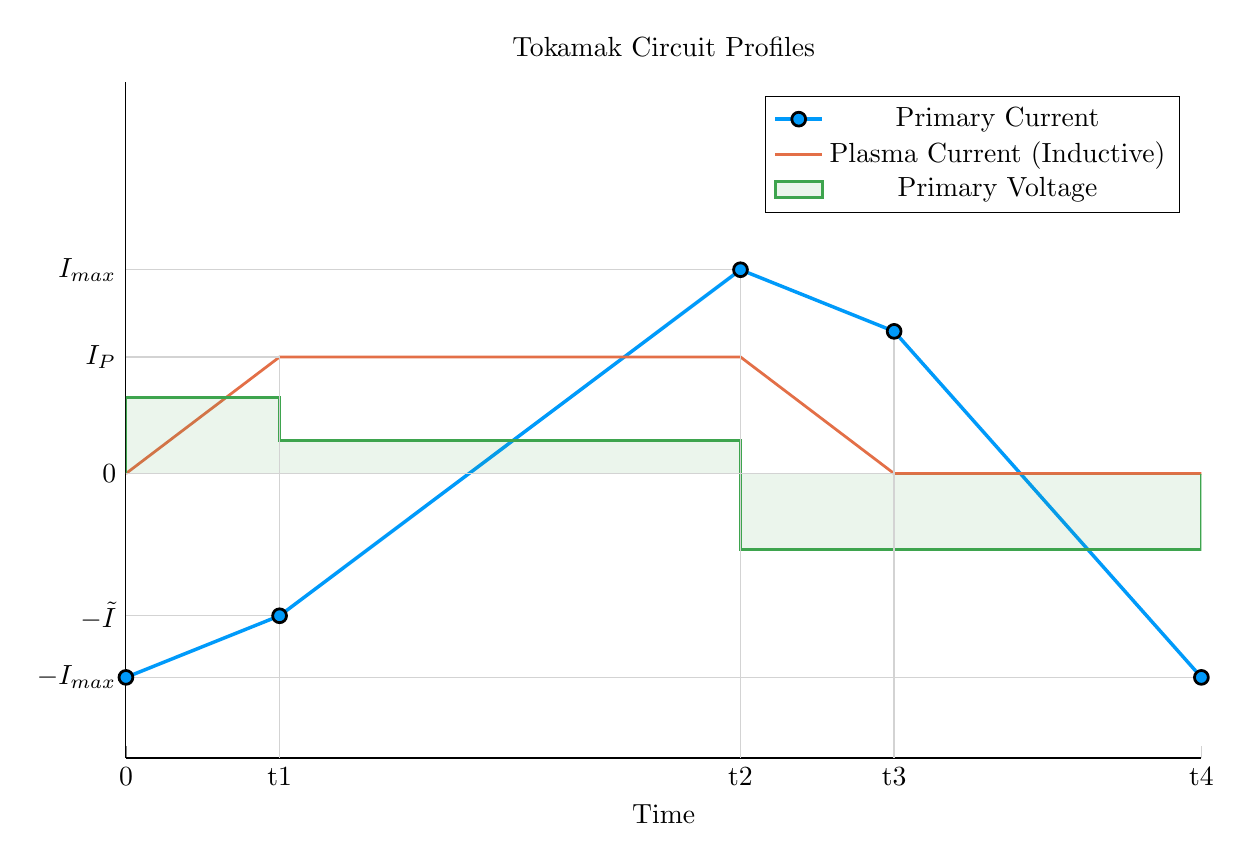
\begin{tikzpicture}[]
\begin{axis}[height = {101.6mm}, ylabel = {}, title = {Tokamak Circuit Profiles}, xmin = {0}, xmax = {7}, ymax = {4.125}, xlabel = {Time}, unbounded coords=jump,scaled x ticks = false,xticklabel style={rotate = 0},xmajorgrids = false,xtick = {0,1,4,5,7},xticklabels = {0,t1,t2,t3,t4},xtick align = inside,axis lines* = left,scaled y ticks = false,yticklabel style={rotate = 0},ymajorgrids = false,ytick = {0.0,-2.15,2.15,1.23,-1.5},yticklabels = {0,${-I_{max}}$,$I_{max}$,$I_P$,${-\tilde{I}}$},ytick align = inside,axis lines* = left,    xshift = 0.0mm,
    yshift = 0.0mm,
    axis background/.style={fill={rgb,1:red,1.00000000;green,1.00000000;blue,1.00000000}}
, ymin = {-3}, width = {152.4mm}]\addplot+ [color = {rgb,1:red,0.00000000;green,0.60560316;blue,0.97868012},
draw opacity=1.0,
line width=1.25,
solid,mark = *,
mark size = 2.5,
mark options = {
    color = {rgb,1:red,0.00000000;green,0.00000000;blue,0.00000000}, draw opacity = 1.0,
    fill = {rgb,1:red,0.00000000;green,0.60560316;blue,0.97868012}, fill opacity = 1.0,
    line width = 1,
    rotate = 0,
    solid
}]coordinates {
(0.0, -2.15)
(1.0, -1.5)
(4.0, 2.15)
(5.0, 1.5)
(7.0, -2.15)
};
\addlegendentry{Primary Current}
\addplot+ [color = {rgb,1:red,0.88887350;green,0.43564919;blue,0.27812294},
draw opacity=1.0,
line width=1,
solid,mark = none,
mark size = 2.0,
mark options = {
    color = {rgb,1:red,0.00000000;green,0.00000000;blue,0.00000000}, draw opacity = 1.0,
    fill = {rgb,1:red,0.88887350;green,0.43564919;blue,0.27812294}, fill opacity = 1.0,
    line width = 1,
    rotate = 0,
    solid
}]coordinates {
(0.0, 0.0)
(1.0, 1.23)
(4.0, 1.23)
(5.0, 0.0)
(7.0, 0.0)
};
\addlegendentry{Plasma Current (Inductive)}
\addplot+ [color = {rgb,1:red,0.24222430;green,0.64327509;blue,0.30444865},
draw opacity=1.0,
line width=1,
solid,mark = none,
mark size = 2.0,
mark options = {
    color = {rgb,1:red,0.00000000;green,0.00000000;blue,0.00000000}, draw opacity = 1.0,
    fill = {rgb,1:red,0.24222430;green,0.64327509;blue,0.30444865}, fill opacity = 1.0,
    line width = 1,
    rotate = 0,
    solid
},fill = {rgb,1:red,0.24222430;green,0.64327509;blue,0.30444865}, fill opacity=0.1,area legend]coordinates {
(0.0, 0.0)
(0.0, 0.8)
(1.0, 0.8)
(1.0, 0.35)
(4.0, 0.35)
(4.0, 0.0)
(NaN, NaN)
(4.0, 0.0)
(4.0, -0.8)
(7.0, -0.8)
(7.0, 0.0)
};
\addlegendentry{Primary Voltage}
\addplot+ [color = {rgb,1:red,0.82745098;green,0.82745098;blue,0.82745098},
draw opacity=1.0,
line width=0.5,
solid,mark = none,
mark size = 2.0,
mark options = {
    color = {rgb,1:red,0.00000000;green,0.00000000;blue,0.00000000}, draw opacity = 1.0,
    fill = {rgb,1:red,0.76444018;green,0.44411178;blue,0.82429754}, fill opacity = 1.0,
    line width = 1,
    rotate = 0,
    solid
},forget plot]coordinates {
(1.0, -4.25)
(1.0, 1.23)
(NaN, NaN)
(4.0, -4.25)
(4.0, 2.15)
(NaN, NaN)
(5.0, -4.25)
(5.0, 1.5)
(NaN, NaN)
(0.0, 1.23)
(1.0, 1.23)
(NaN, NaN)
(0.0, 2.15)
(4.0, 2.15)
(NaN, NaN)
(0.0, -1.5)
(1.0, -1.5)
(NaN, NaN)
(0.0, 0.0)
(5.0, 0.0)
(NaN, NaN)
(0.0, -2.15)
(7.0, -2.15)
};
\end{axis}

\end{tikzpicture}

\end{adjustbox}

\caption{Time Evolution of Circuit Profiles}
\label{fig:circuit_profiles}
\end{figure}

Transformer pulses between the central solenoid and the plasma occur on the timescale of hours. For clarity, each pulse is subdivided into four phases: ramp-up, flattop, ramp-down, and dwell. Pictorially represented in \cref{fig:circuit_profiles}, these divisions allow a simple scheme for transforming the coupled circuit differential equations -- from \cref{eq:circ1,eq:circ2} -- into simple algebraic formulas. 

Along the way, we will approximate derivatives with linear piecewise functions. Using $t_i$ to represent the initial time and $t_f$ the final one, this can be written as:

\begin{equation}
	\dot I = \frac{ I(t_f) - I(t_i) }{t_f - t_i}
\end{equation}

In tabular form, the data from \cref{fig:circuit_profiles} can be written in a piecewise fashion as:

\begin{table}[h!]
\centering	
\caption{Piecewise Linear Scheme for Pulsed Operation}
\hfill
\begin{subtable}[t]{0.4\textwidth}
\centering	
\caption{Currents} ~\\
\begin{tabular}{ c|c|c } 

\textbf{Time} & {$\bold{I_1}$} & {$\bold{I_2}$} \\
\hline
0 & $-I_{max}$ & 0 \\ 
t1 & $-\tilde I \ \ \ \,\, $ & $I_P^{\,*} $ \\ 
t2 & $+I_{max}$ & $I_P^{\,*}$ \\ 
t3 & $+\tilde I \ \ \ \,\, $ & 0 \\ 
t4 & $-I_{max}$ & 0 \\ 
\end{tabular}
\end{subtable}
\hfill
\begin{subtable}[t]{0.5\textwidth}
\centering	
\caption{Voltage} ~\\
\begin{tabular}{ c|c|c|c } 
\textbf{Phase} & $\bold{t_i}$ & $\bold{t_f}$ & $\bold{V_1}$ \\
\hline
Ramp-Up & 0 & $t_1$ & $+V_{max}$ \\ 
Flattop & $t_1$ & $t_2$ & $+ \tilde V$ \ \,\,\, \\ 
Ramp-Down & $t_2$ & $t_3$ & ${-V}_{max}$ \\ 
Dwell & $t_3$ & $t_4$ & ${-V}_{max}$ \\ 
\end{tabular}
\end{subtable}
\hfill
\hfill
\end{table}

\subsubsection{The Ramp-Up Phase -- RU}

The first phase in every plasma pulse is the ramp-up. During ramp-up, the central solenoid starts discharging from its fully charged values, as the plasma is brought to a quasi-steady-state current. As this occurs on the timescale of minutes -- not hours -- resistive effects of the plasma can safely be ignored. This results in the ramp-up equations becoming:

\begin{align}
	V_{max} = \frac{1}{\tau_{RU}} \cdot \left( L_1 \cdot ( I_{max} - \tilde I ) - M \cdot I_{ID} \right) \\
	0 = \frac{1}{\tau_{RU}} \cdot \left( M \cdot ( I_{max} - \tilde I ) - L_2 \cdot I_{ID} \right)
\end{align}

Simplifying these equations will be done shortly, for now the new terms are what is important. The maximum voltage of the solenoid is $V_{max}$. Then, $I_{max}$ is the solenoid's current at the beginning of ramp-up, whereas $\tilde I$ is the magnitude of its current once the plasma is at its flattop inductive-drive current -- $I_{ID}$. Next, the $\tau_{RU}$ quantity is the duration of time it takes to ramp-up (i.e. RU). Again, $L_1$ and $L_2$ are the internal inductances of the solenoid and plasma, respectively, and M is the mutual inductance between them.

The last step in discussing ramp-up is giving the two important formulas that come from it:

\begin{equation}
	\tilde I = I_{max} - I_{ID} \cdot \left( \frac{L_2}{M} \right)
\end{equation}

\begin{equation}
	\label{eq:tauru}
	\tau_{RU} = \frac{I_{ID}}{V_{max}} \cdot \left( \frac{ L_1 L_2 - M^2 }{ M } \right)
\end{equation}

\subsubsection{The Flattop Phase -- FT}

The most important phase in any reactor's pulse is flattop -- the quasi-steady-state time when the tokamak is making electricity (and money). Flattops are assumed to last a couple of hours for a profitable machine, during which the central solenoid completely discharges to overcome a plasma's resistive losses -- keeping it in a quasi-steady-state mode of operation. In a steady-state reactor, this phases constitutes the entirety of the pulse.

Although the resistance cannot be safely neglected for flattop -- as it was for ramp-up -- the plasma's inductive current ($I_{ID}$) is assumed constant. This leads to its derivative in equations cancelling out! Mathematically,

\begin{align}
	\tilde V = \frac{L_1}{\tau_{FT}} \cdot \left( I_{max} + \tilde I \right) \\
	I_{ID} R_P = \frac{M}{\tau_{FT}} \cdot \left( I_{max} + \tilde I \right)
\end{align}

As with ramp-up, the simplifications will be given shortly. The new terms here, however, are an intermediate voltage for the central solenoid ($\tilde V$), and the duration of the flattop ($\tau_{FT}$). The resistance term was given in \cref{eq:rp}. Solutions can then be found by substituting $\tilde I$ into the flattop equations:

\begin{equation}
	\tilde V = I_{ID} R_P \cdot \left( \frac{L_1}{M} \right)	
\end{equation}

\begin{equation}
	\label{eq:tauft}
	\tau_{FT} = \frac{ I_{max} \cdot 2 M - I_{ID} \cdot  L_2 }{I_{ID} R_P}
\end{equation}

\subsubsection{The Ramp-Down Phase -- RD}

Due to the simplicity -- and symmetry -- of the reactor pulse, ramp-down is the exact mirror of ramp-up. It takes the same amount of time and results in the same algebraic equations. For brevity, this will just be represented as:

\begin{equation}
	\label{eq:taurd}
	\tau_{RD} = \tau_{RU}
\end{equation}

For clarity, this is the time when a plasma's current is brought down from its flattop value to zero.

\subsubsection{The Dwell Phase -- DW}

Where the first three phases had little ambiguity, the dwell phase changes definition from model to model. For now, it is assumed to be the time it takes the central solenoid to reset after a plasma has been completely ramped-down to an off-mode. To get a more realistic duty factor for cost estimates, it could include an evacuation time, set to last around thirty minutes. During this evacuation, a plasma is vacuumed out of a device as it undergoes some inter-pulse maintenance.

Ignoring evacuation for now, the dwell phase involves resetting the central solenoid when the plasma's current is negligible. This fundamentally means the secondary of the transformer is nonexistent -- the central solenoid is the entire circuit. In equation form,

\begin{equation}
	V_{max} = \frac{L_1}{\tau_{DW}} \cdot \left( I_{max} + \tilde I \right) 
\end{equation}

Or substituting in $\tilde I$ and solving for $\tau_{DW}$,

\begin{equation}
	\label{eq:taudw}
	\tau_{DW} = \frac{L_1}{M} \cdot \frac{ \left( I_{max} \cdot 2 M - I_{ID} \cdot  L_2 \right) }{V_{max}}
\end{equation}

\subsection{Specifying Circuit Variables}

The goal now is to collect the results from the four phases and introduce the inductance, resistance, voltage, and current terms relevant to this model. This will motivate recasting the problem as flux balance in a reactor -- the form commonly used in the literature (and discussed next section).

First, collecting the phase durations in one place:

\begin{align}
	\tag{\ref{eq:tauru}}
	\tau_{RU} &= \frac{I_{ID}}{V_{max}} \cdot \left( \frac{ L_1 L_2 - M^2 }{ M } \right) \\
	\tag{\ref{eq:tauft}}
	\tau_{FT} &= \frac{ I_{max} \cdot 2 M - I_{ID} \cdot  L_2 }{I_{ID} R_P} \\
	\tag{\ref{eq:taurd}}
	\tau_{RD} &= \tau_{RU} \\
	\tag{\ref{eq:taudw}}
	\tau_{DW} &= \frac{L_1}{M} \cdot \frac{ \left( I_{max} \cdot 2 M - I_{ID} \cdot  L_2 \right) }{V_{max}}
\end{align}

These can be used in the definition of the duty-factor: the percentage of time a reactor is putting electricity on the grid. Formulaically,

\begin{equation}
	\label{eq:duty}
	f_{duty} = \frac{\tau_{FT}}{\tau_{pulse}}
\end{equation}

\begin{equation}
	\tau_{pulse} = \tau_{RU} + \tau_{FT} + \tau_{RD} + \tau_{DW}
\end{equation}

As will turn out, the solving of pulsed current actually only involves \cref{eq:tauft}. What is interesting about this, is it has no explicit dependence on ramp-down or dwell! Whereas ramp-up passes $\tilde I$ to the flattop phase, the other two are just involved in calculating the duty factor.

The remainder of this subsection will then be defining the following circuit variables: $I_{ID}$, $I_{max}$, $V_{max}$, $L_1$, $L_2$, and $M$.

\subsubsection{The Inductive Current -- $I_D$}

The inductive current is the source of current that separates pulsed from steady-state operation. Quickly fitting it into the previous definitions of current balance:

\begin{equation}
	I_{ID} = I_P - ( I_{BS} + I_{CD} )
\end{equation}

As before, $I_P$ is the total plasma current in mega-amps, $I_{BS}$ is the bootstrap current, and $I_{CD}$ is the current from LHCD (i.e. lower hybrid current drive). For this model, the relation can be rewritten as:

\begin{equation}
	I_{ID} = I_P \cdot \Big( 1 - K_{CD} ( \sigma v ) \Big) - K_{BS} \, \overline T
\end{equation}

\subsubsection{The Central Solenoid Maximums -- $V_{max}$ and $I_{max}$}

For this simple model, the central solenoid has two maximum values: the voltage and current. The voltage is the easier to give value. Literature values have this around:

\begin{equation}
	V_{max} \approx 5 \, \textnormal{kV}
\end{equation}

The maximum current, on the other hand, can be defined through Ampere's Law on a helically-shaped central solenoid:

\begin{equation}
	I_{max} = \frac{B_{CS} h_{CS}}{N \mu_0}
\end{equation}

Here, $B_{CS}$ is a magnetic field strength the central solenoid is assumed to operate at (i.e. 20 T), $h_{CS}$ is the height of the solenoid, N is the number of loops, and $\mu_0$ has its usual physics meaning $\left( \textnormal{i.e.} \ 40 \, \pi \, \frac{ \mu \textnormal{H}}{\textnormal{m}} \right)$. As will be seen, the value of N does not affect the model, as it cancels out in the final flux balance. The height of the central solenoid will be the focus of a future section on an in-depth look at tokamak geometry.

\subsubsection{The Central Solenoid Inductance -- $L_1$}

For a central solenoid with circular cross-sections of finite thickness (d), the inductance can be written as:

\begin{equation}
	L_1 = G_{LT} \cdot \left( \frac{\mu_0 \pi N^2}{h_{CS}} \right)
\end{equation}

\begin{equation}
	G_{LT} = \frac{R_{CS}^2 + R_{CS} \cdot ( R_{CS} + d ) + ( R_{CS} + d ) ^ 2 }{3}
\end{equation}

Note that $R_{CS}$ is the inner radius of the central solenoid and $( R_{CS} + d )$ is the outer one. In the limit where d is negligible, this says the inductance is quadratically dependent on the radius of the solenoid, as

\begin{equation}
	\label{eq:glt_simple}
	\underset{d \to 0}{\lim} \ G_{LT} = G_{LT}^{\,\dagger} = R_{CS}^2
\end{equation}

The formulas for both $R_{CS}$ and d will be defined in a few sections.

\subsubsection{The Plasma Inductance -- $L_2$}

The plasma inductance is a composite of several different terms, but overall scales with radius. Through equation,

\begin{equation}
	L_2 = K_{LP} R_0
\end{equation}

This fixed coefficient -- $K_{LP}$ -- then combines three inductive behaviors of the plasma. The first is its own self inductance (through $l_i$). The next is a resistive component through the Ejima coefficient, $C_{ejima}$, which is usually set to $\sim \frac{1}{3}$. And lastly, a geometric component -- involving $\epsilon$ and $\kappa$ -- given by the Hirshman-Neilson model. Mathematically,

\begin{equation}
	K_{LP} = \mu_0 \cdot \left( \frac{l_i}{2} + C_{ejima} + \frac{ ( b_{HN} - a_{HN} ) \, ( 1 - \epsilon ) }{ ( 1 - \epsilon ) + \kappa \, d_{HN} } \right)
\end{equation}

Here the HN values come from the 1985 Hirshman-Neilson paper:

\begin{equation}
	a_{HN}(\epsilon) = 2.0 + 9.25 \sqrt{\epsilon} - 1.21 \, \epsilon
\end{equation}

\begin{equation}
	b_{HN}(\epsilon) = \textnormal{ln} (8/\epsilon) \cdot ( 1 + 1.81 \sqrt{\epsilon} + 2.05 \, \epsilon )
\end{equation}

\begin{equation}
	d_{HN}(\epsilon) = 0.73 \sqrt{\epsilon}  \cdot ( 1 + 2 \epsilon^4 - 6 \epsilon^5 +3.7 \epsilon^6 )
\end{equation}

\subsubsection{The Mutual Inductance -- M}

The mutual inductance -- M -- represents the coupling between the solenoid primary and the plasma secondary. A common method for treating this mutual inductance is through a coupling coefficient, k, that links the two self-inductances. Formulaically, 

\begin{equation}
	M = k \sqrt{ L_1 L_2 }
\end{equation}

The value of the coupling coefficient, k, is always less than (or equal to) 1, but usually has a value around one-third. With all the equations defined, we are now at a position to explain one of the larger nuances of this fusion systems framework: declaring the pulse length of a tokamak.

\subsection{Reasoning the Pulse Length}

\label{section:pulse}

This subsection focuses on a quantitative estimate for how to select a pulse length. As no fusion reactor exists in the world today, the writers believed this to be an acceptable calculation. Further, the resulting length of two hours matches the length of other studies in the literature.

Starting at the end, our goal is to find the pulse length of a tokamak reactor in seconds.  The first piece of information is the expected lifetime of the central solenoid, $ N \approx 10 \ \textnormal{years} $. The next is the desired number of shots the machine will likely have, $ M \approx 50,000 \ \textnormal{shots} $. This gives the ballpark estimate of around 10 pulses a day -- or a pulse length of two hours.

With the pulse length defined, we are now in a position to justify neglecting the duty factor for pulsed reactors in this model. Using ballpark reactor values -- while assuming the central solenoid has around 4000 turns -- leads to the following scalings:

\begin{equation}
	\tau_{FT} \sim \tau_{pulse} \sim \textnormal{O(hours)}
\end{equation}

\begin{equation}
	\tau_{RU} \sim \tau_{RD} \sim \tau_{DW} \sim \textnormal{O(mins)}
\end{equation}

As such, even pulsed tokamak reactors should have a duty factor of around unity:

\begin{equation}
	f_{duty} \approx 1
\end{equation}

Now that all the terms in a pulsed circuit have been explored, we will move on to rearranging the flattop equation to reproduce flux balance. This will then naturally lead to a generalized current equation -- the main goal of this chapter.

\section{Salvaging Flux Balance}

The goal of this section is to arrive at a conservation equation for flux balance that mirrors the ones in the literature. The fusion systems model this one attempts to follow most is the PROCESS code.\cite{process} In a manner similar to power balance, flux balance can be written as:

\begin{equation}
	\sum_{sources} \Phi = \sum_{sinks} \, \Phi
\end{equation}

\subsection{Rearranging the Circuit Equation}

The way to arrive at flux balance from the circuit equation is then to rearrange the flattop phase's duration equation:

\begin{equation}
	\tag{\ref{eq:tauft}}
	\tau_{FT} = \frac{ I_{max} \cdot 2 M - I_{ID} \cdot  L_2 }{I_{ID} R_P}
\end{equation}

Multiplying by the right-hand side's denominator and moving the negative term over yields:

\begin{equation}
	2 M I_{max} = I_{ID} \cdot \left( L_2 + R_P \tau_{FT} \right) 
\end{equation}

This equation is flux balance, where the left-hand side are the sources (e.g. the central solenoid), and the other terms are the sinks (i.e. ramp-up and flattop). The source term can currently be encapsulated in:

\begin{equation}
	\label{eq:phics}
	\Phi_{CS} = 2 M I_{max}
\end{equation}

The sinks, namely the ramp-up inductive losses ($\Phi_{RU}$) and the flattop resistive losses ($\Phi_{FT}$) losses, are what drain up the flux. Again, ramp-down and dwell are not included as sinks because flux balance only tracks till the end of flattop. They come into play when measuring the cost of electricity -- with the duty factor from \cref{eq:duty}.

Relabeling terms, flux balance now has the form:

\begin{equation}
	\Phi_{CS} = \Phi_{RU} + \Phi_{FT}
\end{equation}

With the ramp-up and flattop flux given respectively by:

\begin{equation}
	\label{eq:phiru}
	\Phi_{RU} = L_2 \cdot I_{ID}
\end{equation}

\begin{equation}
	\label{eq:phift}
	\Phi_{FT} = ( R_P \tau_{FT} ) \cdot I_{ID}
\end{equation}

On comparing these quantities to the ones from the PROCESS team, $\Phi_{RU}$ and $\Phi_{FT}$ are exactly the same. The source terms, on the other hand, are off for two reasons -- both related to the central solenoid being the only source term in flux balance. This can partially be remedied by adding the second most dominant source of flux a posteriori -- i.e. the PF coils. The second, and inherently limiting factor, is the simplicity of the current model. All that can be shown to that regard is the $\Phi_{CS}$ terms do reasonably predict the values from PROCESS (see the results chapter).

\subsection{Importing Poloidal Field Coils}

Adding the effect of PF coils -- belts of current driving plates on the outer edges of the tokamak -- leads to a second-order improvement over relying solely on the central solenoid for flux generation. From the literature, this can be modeled as:

\begin{equation}
	\label{eq:phipf}
	\Phi_{PF} = \pi B_V \cdot \left( R_0^2 - ( R_{CS} + d ) ^ 2 \right)
\end{equation}

Where again $R_{CS}$ and $d$ are the inner radius and thickness of the central solenoid, respectively. These will be the topic of the next section.

Moving forward, the vertical field -- $B_V$ -- is a magnetic field oriented up-and-down with the ground. It is needed to prevent a tokamak plasma from spinning out of the machine. From the literature, the magnitude of this vertical field is given by:

\begin{equation}
  |B_V| = \frac{\mu_0 I_P}{4 \pi R_0} \cdot \left( \,\textnormal{ln} \left(\frac{8}{\epsilon}\right) + \beta_{\,p} + \frac{l_i}{2} - \frac{3}{2} \, \right)
\end{equation} 

Analogous to the previously covered plasma beta, the poloidal beta can be represented by:

\begin{equation}
  \beta_p = \frac{\overline{p}}{\left( \frac{\overline{B_p}^{\,2}}{2 \mu_0} \right)}
\end{equation}

Where the average poloidal magnetic field comes from a simple application of Ampere's law:

\begin{equation}
	\overline{B_p} = \frac{\mu_0 I_P}{l_p}
\end{equation}

The variable $l_p$ is then the perimeter of the tokamak's cross-sectional halves:

\begin{equation}
	l_p = 2 \pi a \cdot \sqrt{g_p}
\end{equation}

Here, $g_p$ is another geometric scaling factor,

\begin{equation}
  g_p = \frac{1 + \kappa^2 ( 1 + 2 \delta^2 - 1.2\delta^3 )}{2} 
\end{equation}

Boiled down, this relation for the magnitude of the vertical magnetic field can be written in standardized units as:

\begin{equation}
	|B_V| = \left( \frac{ 1 }{ 10 \cdot R_0} \right) \cdot \left( K_{VI} I_P +  K_{VT\,} \overline{T}  \right)
\end{equation}

\begin{equation}
	K_{VT} = K_{n} \cdot ( \epsilon ^ 2 \, g_P ) \cdot ( 1 + f_D ) \, \frac{ (1 + \nu_n) \, (1 + \nu_T) }{1 + \nu_n + \nu_T }
\end{equation}

\begin{equation}
	K_{VI} = \textnormal{ln} \left(\frac{8}{\epsilon}\right) + \frac{l_i}{2} - \frac{3}{2}
\end{equation}

For clarity, this will be plugged into the new PF coil flux contribution ($\Phi_{PF}$):

\begin{equation}
	\tag{\ref{eq:phipf}}
	\Phi_{PF} = \pi B_V \cdot \left( R_0^2 - ( R_{CS} + d ) ^ 2 \right)
\end{equation}

Which then gets plugged into a more complete flux balance:

\begin{equation}
	\label{eq:full_ibal}
	\Phi_{CS} + \Phi_{PF} = \Phi_{RU} + \Phi_{FT}
\end{equation}

The $R_{CS}$ and $d$ terms found in $\Phi_{PF}$ will now be discussed as they are needed for this more sophisticated tokamak geometry.

\section{Improving Tokamak Geometry}

From before, this fusion systems model has been said to depend on the major and minor radius -- $R_0$ and $a$, respectively -- and along the way, various geometric parameters have been defined (e.g. $\epsilon$, $\kappa$, $\delta$) to describe the geometry further. Now three more thicknesses will be added: $b$, $c$, and $d$. Additionally, two fundamental dimension corresponding to the solenoid will be added: the radius and height -- $R_{CS}$ and $h_{CS}$, respectively. These are the topics of this section.

\subsection{Defining Central Solenoid Dimensions}

The best way to conceptualize tokamak geometry is through cartoon -- see \cref{fig:dims}. What this says is there is a gap at the very center of a tokamak. This gap extends radially outwards to $R_{CS}$ meters where the slinky-shaped central solenoid -- of thickness $d$ -- begins. Between the outer edge of the solenoid and the wall of the torus (i.e. the doughnut) are the blanket and toroidal field (TF) coils.

\begin{figure*}
\centering
\begin{adjustbox}{width=0.85\textwidth}
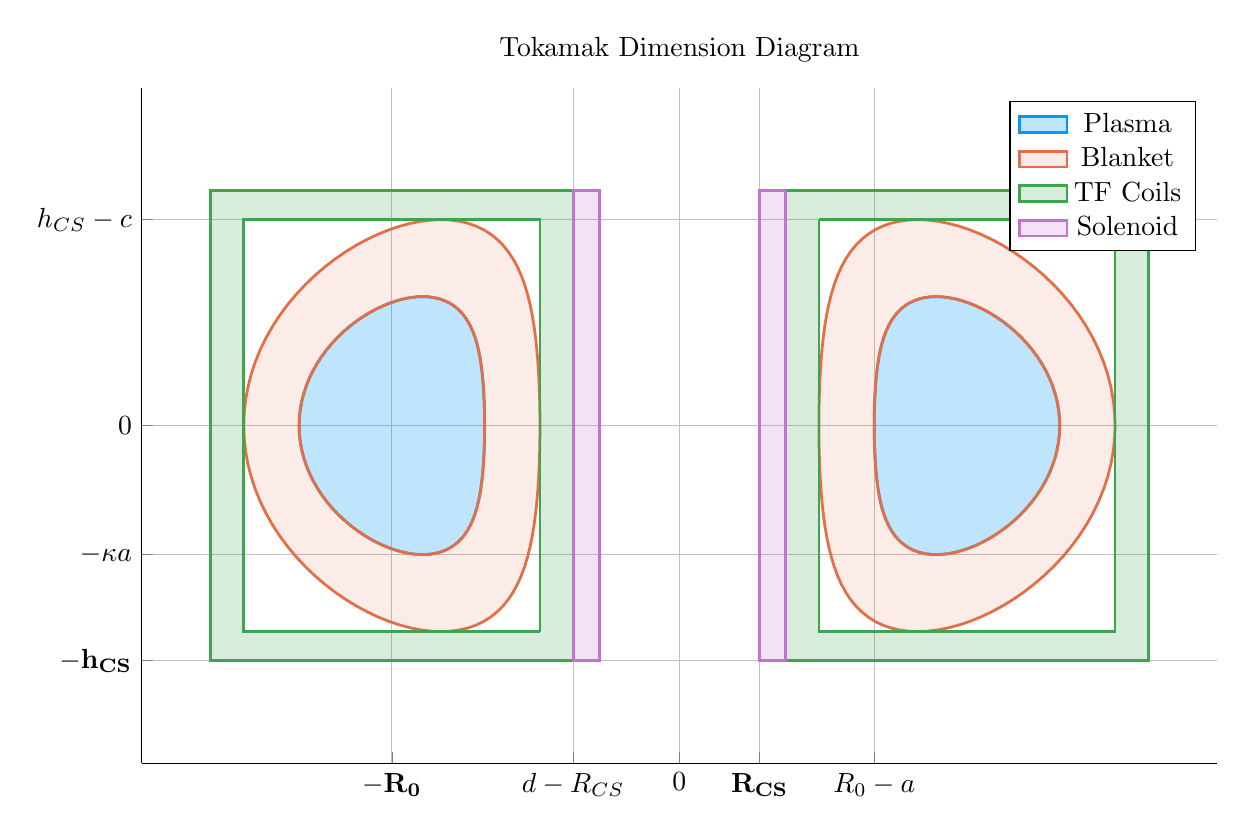
\begin{tikzpicture}[]
\begin{axis}[height = {101.6mm}, ylabel = {}, title = {Tokamak Dimension Diagram}, xmin = {-16.96464}, xmax = {16.96464}, ymax = {12.181706012903225}, xlabel = {}, unbounded coords=jump,scaled x ticks = false,xticklabel style={rotate = 0},xmajorgrids = true,xtick = {0.0,2.5317214541730677,-9.072,6.145548387096774,-3.3497214541730678},xticklabels = {0,$\bf{R_{CS}}$,$\bf{{-R}_0}$,$R_0 - a$,$d - R_{CS}$},xtick align = inside,axis lines* = left,scaled y ticks = false,yticklabel style={rotate = 0},ymajorgrids = true,ytick = {0.0,-8.478922887864822,-4.653058064516129,7.428922887864823},yticklabels = {0,$\bf{{-h}_{CS}}$,${-\kappa} a$,$h_{CS} - c$},ytick align = inside,axis lines* = left,    xshift = 0.0mm,
    yshift = 0.0mm,
    axis background/.style={fill={rgb,1:red,1.00000000;green,1.00000000;blue,1.00000000}}
, ymin = {-12.181706012903225}, width = {152.4mm}]\addplot+ [color = {rgb,1:red,0.00000000;green,0.60560316;blue,0.97868012},
draw opacity=1.0,
line width=1,
solid,mark = none,
mark size = 2.0,
mark options = {
    color = {rgb,1:red,0.00000000;green,0.00000000;blue,0.00000000}, draw opacity = 1.0,
    fill = {rgb,1:red,0.00000000;green,0.60560316;blue,0.97868012}, fill opacity = 1.0,
    line width = 1,
    rotate = 0,
    solid
},fill = {rgb,1:red,0.00000000;green,0.60560316;blue,0.97868012}, fill opacity=0.25,area legend]coordinates {
(-11.998451612903224, 0.0)
(-11.98922207919679, 0.2921679332710291)
(-11.961601612443932, 0.5831828131882695)
(-11.915794116436746, 0.8718961369727396)
(-11.852137762522407, 1.1571684850360338)
(-11.771102473770108, 1.4378740177488842)
(-11.673286377647635, 1.7129049186158334)
(-11.55941120568557, 1.9811757663208256)
(-11.430316617462449, 2.241627818389261)
(-11.286953428530017, 2.4932331895608506)
(-11.130375728034215, 2.7349989083831394)
(-10.96173188200961, 2.9659708360161865)
(-10.782254432669117, 3.1852374317826615)
(-10.59324892230544, 3.391933350602452)
(-10.396081692289423, 3.58524285811436)
(-10.192166732519574, 3.7644030500069485)
(-9.982951683794182, 3.9287068628533244)
(-9.769903124035281, 4.0775058645674545)
(-9.554491298062636, 4.21021281346937)
(-9.338174478579997, 4.326303975859794)
(-9.122383172034585, 4.425321192957779)
(-8.908504405883159, 4.5068736890441015)
(-8.697866352426912, 4.570639613674501)
(-8.491723557735288, 4.616367311876341)
(-8.2912430513685, 4.643876317315818)
(-8.097491612903225, 4.653058064516129)
(-7.911424464141755, 4.643876317315818)
(-7.73387564104738, 4.616367311876341)
(-7.565550276852846, 4.570639613674501)
(-7.4070189976483904, 4.506873689044102)
(-7.258714594546428, 4.42532119295778)
(-7.120931092970638, 4.326303975859795)
(-6.993825290693801, 4.21021281346937)
(-6.877420783129728, 4.077505864567455)
(-6.771614438426758, 3.928706862853325)
(-6.676185227609827, 3.7644030500069485)
(-6.590805257964794, 3.58524285811436)
(-6.515052802686304, 3.391933350602452)
(-6.448427068145589, 3.1852374317826624)
(-6.390364393542622, 2.9659708360161874)
(-6.340255537642832, 2.73499890838314)
(-6.297463675055492, 2.4932331895608506)
(-6.261342701178994, 2.241627818389261)
(-6.231255431364441, 1.9811757663208265)
(-6.206591276608178, 1.7129049186158343)
(-6.186782985455325, 1.4378740177488847)
(-6.171322059752492, 1.1571684850360338)
(-6.159772480089943, 0.8718961369727395)
(-6.151782414579849, 0.5831828131882707)
(-6.147093631099405, 0.29216793327103)
(-6.145548387096774, 5.698352664956456e-16)
(-6.147093631099405, -0.2921679332710289)
(-6.151782414579849, -0.5831828131882696)
(-6.159772480089943, -0.8718961369727383)
(-6.171322059752492, -1.1571684850360326)
(-6.1867829854553245, -1.4378740177488838)
(-6.206591276608178, -1.7129049186158334)
(-6.231255431364441, -1.9811757663208256)
(-6.261342701178992, -2.2416278183892597)
(-6.297463675055493, -2.4932331895608497)
(-6.340255537642832, -2.734998908383139)
(-6.390364393542622, -2.9659708360161865)
(-6.448427068145589, -3.185237431782662)
(-6.515052802686304, -3.3919333506024514)
(-6.590805257964794, -3.5852428581143605)
(-6.676185227609827, -3.7644030500069485)
(-6.771614438426755, -3.928706862853323)
(-6.877420783129727, -4.0775058645674545)
(-6.9938252906938, -4.21021281346937)
(-7.120931092970639, -4.326303975859795)
(-7.258714594546428, -4.425321192957779)
(-7.407018997648389, -4.5068736890441015)
(-7.565550276852846, -4.570639613674501)
(-7.733875641047377, -4.616367311876341)
(-7.9114244641417555, -4.643876317315818)
(-8.097491612903225, -4.653058064516129)
(-8.291243051368498, -4.643876317315818)
(-8.491723557735288, -4.616367311876341)
(-8.69786635242691, -4.570639613674501)
(-8.90850440588316, -4.5068736890441015)
(-9.122383172034585, -4.42532119295778)
(-9.338174478579994, -4.326303975859796)
(-9.554491298062636, -4.21021281346937)
(-9.76990312403528, -4.077505864567455)
(-9.982951683794184, -3.928706862853324)
(-10.192166732519574, -3.7644030500069494)
(-10.396081692289421, -3.5852428581143614)
(-10.59324892230544, -3.391933350602452)
(-10.782254432669115, -3.1852374317826624)
(-10.96173188200961, -2.9659708360161865)
(-11.130375728034215, -2.7349989083831403)
(-11.286953428530017, -2.493233189560853)
(-11.430316617462449, -2.241627818389261)
(-11.559411205685569, -1.981175766320827)
(-11.673286377647635, -1.7129049186158327)
(-11.771102473770108, -1.4378740177488853)
(-11.852137762522407, -1.1571684850360362)
(-11.915794116436746, -0.8718961369727398)
(-11.961601612443932, -0.5831828131882713)
(-11.98922207919679, -0.2921679332710286)
(-11.998451612903224, -1.1396705329912913e-15)
(NaN, NaN)
(11.998451612903224, 0.0)
(11.98922207919679, 0.2921679332710291)
(11.961601612443932, 0.5831828131882695)
(11.915794116436746, 0.8718961369727396)
(11.852137762522407, 1.1571684850360338)
(11.771102473770108, 1.4378740177488842)
(11.673286377647635, 1.7129049186158334)
(11.55941120568557, 1.9811757663208256)
(11.430316617462449, 2.241627818389261)
(11.286953428530017, 2.4932331895608506)
(11.130375728034215, 2.7349989083831394)
(10.96173188200961, 2.9659708360161865)
(10.782254432669117, 3.1852374317826615)
(10.59324892230544, 3.391933350602452)
(10.396081692289423, 3.58524285811436)
(10.192166732519574, 3.7644030500069485)
(9.982951683794182, 3.9287068628533244)
(9.769903124035281, 4.0775058645674545)
(9.554491298062636, 4.21021281346937)
(9.338174478579997, 4.326303975859794)
(9.122383172034585, 4.425321192957779)
(8.908504405883159, 4.5068736890441015)
(8.697866352426912, 4.570639613674501)
(8.491723557735288, 4.616367311876341)
(8.2912430513685, 4.643876317315818)
(8.097491612903225, 4.653058064516129)
(7.911424464141755, 4.643876317315818)
(7.73387564104738, 4.616367311876341)
(7.565550276852846, 4.570639613674501)
(7.4070189976483904, 4.506873689044102)
(7.258714594546428, 4.42532119295778)
(7.120931092970638, 4.326303975859795)
(6.993825290693801, 4.21021281346937)
(6.877420783129728, 4.077505864567455)
(6.771614438426758, 3.928706862853325)
(6.676185227609827, 3.7644030500069485)
(6.590805257964794, 3.58524285811436)
(6.515052802686304, 3.391933350602452)
(6.448427068145589, 3.1852374317826624)
(6.390364393542622, 2.9659708360161874)
(6.340255537642832, 2.73499890838314)
(6.297463675055492, 2.4932331895608506)
(6.261342701178994, 2.241627818389261)
(6.231255431364441, 1.9811757663208265)
(6.206591276608178, 1.7129049186158343)
(6.186782985455325, 1.4378740177488847)
(6.171322059752492, 1.1571684850360338)
(6.159772480089943, 0.8718961369727395)
(6.151782414579849, 0.5831828131882707)
(6.147093631099405, 0.29216793327103)
(6.145548387096774, 5.698352664956456e-16)
(6.147093631099405, -0.2921679332710289)
(6.151782414579849, -0.5831828131882696)
(6.159772480089943, -0.8718961369727383)
(6.171322059752492, -1.1571684850360326)
(6.1867829854553245, -1.4378740177488838)
(6.206591276608178, -1.7129049186158334)
(6.231255431364441, -1.9811757663208256)
(6.261342701178992, -2.2416278183892597)
(6.297463675055493, -2.4932331895608497)
(6.340255537642832, -2.734998908383139)
(6.390364393542622, -2.9659708360161865)
(6.448427068145589, -3.185237431782662)
(6.515052802686304, -3.3919333506024514)
(6.590805257964794, -3.5852428581143605)
(6.676185227609827, -3.7644030500069485)
(6.771614438426755, -3.928706862853323)
(6.877420783129727, -4.0775058645674545)
(6.9938252906938, -4.21021281346937)
(7.120931092970639, -4.326303975859795)
(7.258714594546428, -4.425321192957779)
(7.407018997648389, -4.5068736890441015)
(7.565550276852846, -4.570639613674501)
(7.733875641047377, -4.616367311876341)
(7.9114244641417555, -4.643876317315818)
(8.097491612903225, -4.653058064516129)
(8.291243051368498, -4.643876317315818)
(8.491723557735288, -4.616367311876341)
(8.69786635242691, -4.570639613674501)
(8.90850440588316, -4.5068736890441015)
(9.122383172034585, -4.42532119295778)
(9.338174478579994, -4.326303975859796)
(9.554491298062636, -4.21021281346937)
(9.76990312403528, -4.077505864567455)
(9.982951683794184, -3.928706862853324)
(10.192166732519574, -3.7644030500069494)
(10.396081692289421, -3.5852428581143614)
(10.59324892230544, -3.391933350602452)
(10.782254432669115, -3.1852374317826624)
(10.96173188200961, -2.9659708360161865)
(11.130375728034215, -2.7349989083831403)
(11.286953428530017, -2.493233189560853)
(11.430316617462449, -2.241627818389261)
(11.559411205685569, -1.981175766320827)
(11.673286377647635, -1.7129049186158327)
(11.771102473770108, -1.4378740177488853)
(11.852137762522407, -1.1571684850360362)
(11.915794116436746, -0.8718961369727398)
(11.961601612443932, -0.5831828131882713)
(11.98922207919679, -0.2921679332710286)
(11.998451612903224, -1.1396705329912913e-15)
};
\addlegendentry{Plasma}
\addplot+ [color = {rgb,1:red,0.88887350;green,0.43564919;blue,0.27812294},
draw opacity=1.0,
line width=1,
solid,mark = none,
mark size = 2.0,
mark options = {
    color = {rgb,1:red,0.00000000;green,0.00000000;blue,0.00000000}, draw opacity = 1.0,
    fill = {rgb,1:red,0.88887350;green,0.43564919;blue,0.27812294}, fill opacity = 1.0,
    line width = 1,
    rotate = 0,
    solid
},fill = {rgb,1:red,0.88887350;green,0.43564919;blue,0.27812294}, fill opacity=0.125,area legend]coordinates {
(-13.74427854582693, 0.0)
(-13.72954296908463, 0.46646592767223927)
(-13.685445019996358, 0.9310909274359673)
(-13.612310244800092, 1.392041336684088)
(-13.510678556994915, 1.8474979947395098)
(-13.381300220642846, 2.2956634222512418)
(-13.225130186826302, 2.734768915024204)
(-13.04332074889991, 3.1630815242866377)
(-12.837212480347718, 3.5789108958472036)
(-12.608323422706404, 3.9806159411507194)
(-12.358336500812388, 4.3666113139049525)
(-12.08908515895104, 4.735373666718153)
(-11.802537234387401, 5.08544766305526)
(-11.500777113966619, 5.4154517207863275)
(-11.185986254387002, 5.724083464660006)
(-10.860422186454013, 6.010124866183653)
(-10.526396166917667, 6.272447050625345)
(-10.18624968693083, 6.510014752166694)
(-9.842330092097374, 6.721890399624077)
(-9.496965613725703, 6.907237816613755)
(-9.152440152411872, 7.065325521558049)
(-8.81096819159381, 7.195529614508949)
(-8.474670248460548, 7.297336239396166)
(-8.14554929092694, 7.370343611982296)
(-7.825468560863273, 7.4142636055216355)
(-7.516131244239631, 7.428922887864823)
(-7.2190624174706315, 7.4142636055216355)
(-6.935593675557043, 7.370343611982296)
(-6.666850811544881, 7.297336239396167)
(-6.4137448687014755, 7.195529614508949)
(-6.176966827400615, 7.065325521558051)
(-5.956986119179431, 6.907237816613756)
(-5.754053082320152, 6.721890399624076)
(-5.568205388501765, 6.510014752166695)
(-5.3992783807260825, 6.272447050625345)
(-5.246919171238659, 6.010124866183653)
(-5.110604257075394, 5.724083464660006)
(-4.989660322779391, 5.4154517207863275)
(-4.88328781734585, 5.085447663055262)
(-4.790586818065825, 4.735373666718154)
(-4.7105846299742, 4.366611313904953)
(-4.642264518129107, 3.9806159411507194)
(-4.584594932698949, 3.578910895847203)
(-4.536558565161822, 3.1630815242866395)
(-4.497180568747824, 2.7347689150242047)
(-4.465555288023927, 2.2956634222512426)
(-4.440870871189059, 1.8474979947395103)
(-4.422431183673739, 1.3920413366840876)
(-4.409674501998921, 0.9310909274359696)
(-4.402188541060726, 0.46646592767224077)
(-4.399721454173068, 9.097806635736167e-16)
(-4.402188541060726, -0.466465927672239)
(-4.409674501998921, -0.9310909274359678)
(-4.422431183673739, -1.392041336684086)
(-4.440870871189059, -1.8474979947395083)
(-4.465555288023926, -2.295663422251241)
(-4.497180568747823, -2.734768915024204)
(-4.536558565161822, -3.1630815242866377)
(-4.5845949326989475, -3.5789108958472013)
(-4.642264518129108, -3.980615941150719)
(-4.7105846299742, -4.3666113139049525)
(-4.790586818065825, -4.735373666718153)
(-4.88328781734585, -5.085447663055261)
(-4.989660322779391, -5.415451720786327)
(-5.110604257075395, -5.724083464660007)
(-5.246919171238659, -6.010124866183653)
(-5.399278380726081, -6.272447050625343)
(-5.568205388501764, -6.510014752166694)
(-5.754053082320152, -6.721890399624076)
(-5.956986119179432, -6.907237816613756)
(-6.176966827400615, -7.065325521558049)
(-6.413744868701472, -7.195529614508947)
(-6.666850811544881, -7.297336239396167)
(-6.935593675557041, -7.370343611982296)
(-7.219062417470632, -7.4142636055216355)
(-7.51613124423963, -7.428922887864823)
(-7.8254685608632695, -7.4142636055216355)
(-8.14554929092694, -7.370343611982296)
(-8.474670248460544, -7.297336239396167)
(-8.810968191593812, -7.195529614508949)
(-9.152440152411872, -7.065325521558051)
(-9.4969656137257, -6.9072378166137565)
(-9.842330092097372, -6.721890399624077)
(-10.186249686930825, -6.510014752166696)
(-10.526396166917669, -6.272447050625344)
(-10.860422186454013, -6.010124866183654)
(-11.185986254386998, -5.724083464660007)
(-11.500777113966619, -5.4154517207863275)
(-11.8025372343874, -5.085447663055262)
(-12.08908515895104, -4.735373666718153)
(-12.358336500812388, -4.366611313904954)
(-12.608323422706402, -3.9806159411507234)
(-12.837212480347718, -3.5789108958472036)
(-13.04332074889991, -3.1630815242866404)
(-13.225130186826302, -2.7347689150242034)
(-13.381300220642846, -2.2956634222512435)
(-13.510678556994915, -1.8474979947395136)
(-13.612310244800092, -1.3920413366840885)
(-13.685445019996358, -0.9310909274359703)
(-13.72954296908463, -0.46646592767223843)
(-13.74427854582693, -1.8195613271472333e-15)
(NaN, NaN)
(13.74427854582693, 0.0)
(13.72954296908463, 0.46646592767223927)
(13.685445019996358, 0.9310909274359673)
(13.612310244800092, 1.392041336684088)
(13.510678556994915, 1.8474979947395098)
(13.381300220642846, 2.2956634222512418)
(13.225130186826302, 2.734768915024204)
(13.04332074889991, 3.1630815242866377)
(12.837212480347718, 3.5789108958472036)
(12.608323422706404, 3.9806159411507194)
(12.358336500812388, 4.3666113139049525)
(12.08908515895104, 4.735373666718153)
(11.802537234387401, 5.08544766305526)
(11.500777113966619, 5.4154517207863275)
(11.185986254387002, 5.724083464660006)
(10.860422186454013, 6.010124866183653)
(10.526396166917667, 6.272447050625345)
(10.18624968693083, 6.510014752166694)
(9.842330092097374, 6.721890399624077)
(9.496965613725703, 6.907237816613755)
(9.152440152411872, 7.065325521558049)
(8.81096819159381, 7.195529614508949)
(8.474670248460548, 7.297336239396166)
(8.14554929092694, 7.370343611982296)
(7.825468560863273, 7.4142636055216355)
(7.516131244239631, 7.428922887864823)
(7.2190624174706315, 7.4142636055216355)
(6.935593675557043, 7.370343611982296)
(6.666850811544881, 7.297336239396167)
(6.4137448687014755, 7.195529614508949)
(6.176966827400615, 7.065325521558051)
(5.956986119179431, 6.907237816613756)
(5.754053082320152, 6.721890399624076)
(5.568205388501765, 6.510014752166695)
(5.3992783807260825, 6.272447050625345)
(5.246919171238659, 6.010124866183653)
(5.110604257075394, 5.724083464660006)
(4.989660322779391, 5.4154517207863275)
(4.88328781734585, 5.085447663055262)
(4.790586818065825, 4.735373666718154)
(4.7105846299742, 4.366611313904953)
(4.642264518129107, 3.9806159411507194)
(4.584594932698949, 3.578910895847203)
(4.536558565161822, 3.1630815242866395)
(4.497180568747824, 2.7347689150242047)
(4.465555288023927, 2.2956634222512426)
(4.440870871189059, 1.8474979947395103)
(4.422431183673739, 1.3920413366840876)
(4.409674501998921, 0.9310909274359696)
(4.402188541060726, 0.46646592767224077)
(4.399721454173068, 9.097806635736167e-16)
(4.402188541060726, -0.466465927672239)
(4.409674501998921, -0.9310909274359678)
(4.422431183673739, -1.392041336684086)
(4.440870871189059, -1.8474979947395083)
(4.465555288023926, -2.295663422251241)
(4.497180568747823, -2.734768915024204)
(4.536558565161822, -3.1630815242866377)
(4.5845949326989475, -3.5789108958472013)
(4.642264518129108, -3.980615941150719)
(4.7105846299742, -4.3666113139049525)
(4.790586818065825, -4.735373666718153)
(4.88328781734585, -5.085447663055261)
(4.989660322779391, -5.415451720786327)
(5.110604257075395, -5.724083464660007)
(5.246919171238659, -6.010124866183653)
(5.399278380726081, -6.272447050625343)
(5.568205388501764, -6.510014752166694)
(5.754053082320152, -6.721890399624076)
(5.956986119179432, -6.907237816613756)
(6.176966827400615, -7.065325521558049)
(6.413744868701472, -7.195529614508947)
(6.666850811544881, -7.297336239396167)
(6.935593675557041, -7.370343611982296)
(7.219062417470632, -7.4142636055216355)
(7.51613124423963, -7.428922887864823)
(7.8254685608632695, -7.4142636055216355)
(8.14554929092694, -7.370343611982296)
(8.474670248460544, -7.297336239396167)
(8.810968191593812, -7.195529614508949)
(9.152440152411872, -7.065325521558051)
(9.4969656137257, -6.9072378166137565)
(9.842330092097372, -6.721890399624077)
(10.186249686930825, -6.510014752166696)
(10.526396166917669, -6.272447050625344)
(10.860422186454013, -6.010124866183654)
(11.185986254386998, -5.724083464660007)
(11.500777113966619, -5.4154517207863275)
(11.8025372343874, -5.085447663055262)
(12.08908515895104, -4.735373666718153)
(12.358336500812388, -4.366611313904954)
(12.608323422706402, -3.9806159411507234)
(12.837212480347718, -3.5789108958472036)
(13.04332074889991, -3.1630815242866404)
(13.225130186826302, -2.7347689150242034)
(13.381300220642846, -2.2956634222512435)
(13.510678556994915, -1.8474979947395136)
(13.612310244800092, -1.3920413366840885)
(13.685445019996358, -0.9310909274359703)
(13.72954296908463, -0.46646592767223843)
(13.74427854582693, -1.8195613271472333e-15)
(NaN, NaN)
(11.998451612903224, -1.1396705329912913e-15)
(11.98922207919679, -0.2921679332710286)
(11.961601612443932, -0.5831828131882713)
(11.915794116436746, -0.8718961369727398)
(11.852137762522407, -1.1571684850360362)
(11.771102473770108, -1.4378740177488853)
(11.673286377647635, -1.7129049186158327)
(11.55941120568557, -1.981175766320827)
(11.430316617462449, -2.241627818389261)
(11.286953428530017, -2.493233189560853)
(11.130375728034215, -2.7349989083831403)
(10.96173188200961, -2.9659708360161865)
(10.782254432669117, -3.1852374317826624)
(10.59324892230544, -3.391933350602452)
(10.396081692289423, -3.5852428581143614)
(10.192166732519574, -3.7644030500069494)
(9.982951683794182, -3.928706862853324)
(9.769903124035281, -4.077505864567455)
(9.554491298062636, -4.21021281346937)
(9.338174478579997, -4.326303975859796)
(9.122383172034585, -4.42532119295778)
(8.908504405883159, -4.5068736890441015)
(8.697866352426912, -4.570639613674501)
(8.491723557735288, -4.616367311876341)
(8.2912430513685, -4.643876317315818)
(8.097491612903225, -4.653058064516129)
(7.911424464141755, -4.643876317315818)
(7.73387564104738, -4.616367311876341)
(7.565550276852846, -4.570639613674501)
(7.4070189976483904, -4.5068736890441015)
(7.258714594546428, -4.425321192957779)
(7.120931092970638, -4.326303975859795)
(6.993825290693801, -4.21021281346937)
(6.877420783129728, -4.0775058645674545)
(6.771614438426758, -3.928706862853323)
(6.676185227609827, -3.7644030500069485)
(6.590805257964794, -3.5852428581143605)
(6.515052802686304, -3.3919333506024514)
(6.448427068145589, -3.185237431782662)
(6.390364393542622, -2.9659708360161865)
(6.340255537642832, -2.734998908383139)
(6.297463675055492, -2.4932331895608497)
(6.261342701178994, -2.2416278183892597)
(6.231255431364441, -1.9811757663208256)
(6.206591276608178, -1.7129049186158334)
(6.186782985455325, -1.4378740177488838)
(6.171322059752492, -1.1571684850360326)
(6.159772480089943, -0.8718961369727383)
(6.151782414579849, -0.5831828131882696)
(6.147093631099405, -0.2921679332710289)
(6.145548387096774, 5.698352664956456e-16)
(6.147093631099405, 0.29216793327103)
(6.151782414579849, 0.5831828131882707)
(6.159772480089943, 0.8718961369727395)
(6.171322059752492, 1.1571684850360338)
(6.1867829854553245, 1.4378740177488847)
(6.206591276608178, 1.7129049186158343)
(6.231255431364441, 1.9811757663208265)
(6.261342701178992, 2.241627818389261)
(6.297463675055493, 2.4932331895608506)
(6.340255537642832, 2.73499890838314)
(6.390364393542622, 2.9659708360161874)
(6.448427068145589, 3.1852374317826624)
(6.515052802686304, 3.391933350602452)
(6.590805257964794, 3.58524285811436)
(6.676185227609827, 3.7644030500069485)
(6.771614438426755, 3.928706862853325)
(6.877420783129727, 4.077505864567455)
(6.9938252906938, 4.21021281346937)
(7.120931092970639, 4.326303975859795)
(7.258714594546428, 4.42532119295778)
(7.407018997648389, 4.506873689044102)
(7.565550276852846, 4.570639613674501)
(7.733875641047377, 4.616367311876341)
(7.9114244641417555, 4.643876317315818)
(8.097491612903225, 4.653058064516129)
(8.291243051368498, 4.643876317315818)
(8.491723557735288, 4.616367311876341)
(8.69786635242691, 4.570639613674501)
(8.90850440588316, 4.5068736890441015)
(9.122383172034585, 4.425321192957779)
(9.338174478579994, 4.326303975859794)
(9.554491298062636, 4.21021281346937)
(9.76990312403528, 4.0775058645674545)
(9.982951683794184, 3.9287068628533244)
(10.192166732519574, 3.7644030500069485)
(10.396081692289421, 3.58524285811436)
(10.59324892230544, 3.391933350602452)
(10.782254432669115, 3.1852374317826615)
(10.96173188200961, 2.9659708360161865)
(11.130375728034215, 2.7349989083831394)
(11.286953428530017, 2.4932331895608506)
(11.430316617462449, 2.241627818389261)
(11.559411205685569, 1.9811757663208256)
(11.673286377647635, 1.7129049186158334)
(11.771102473770108, 1.4378740177488842)
(11.852137762522407, 1.1571684850360338)
(11.915794116436746, 0.8718961369727396)
(11.961601612443932, 0.5831828131882695)
(11.98922207919679, 0.2921679332710291)
(11.998451612903224, 0.0)
(NaN, NaN)
(-11.998451612903224, -1.1396705329912913e-15)
(-11.98922207919679, -0.2921679332710286)
(-11.961601612443932, -0.5831828131882713)
(-11.915794116436746, -0.8718961369727398)
(-11.852137762522407, -1.1571684850360362)
(-11.771102473770108, -1.4378740177488853)
(-11.673286377647635, -1.7129049186158327)
(-11.55941120568557, -1.981175766320827)
(-11.430316617462449, -2.241627818389261)
(-11.286953428530017, -2.493233189560853)
(-11.130375728034215, -2.7349989083831403)
(-10.96173188200961, -2.9659708360161865)
(-10.782254432669117, -3.1852374317826624)
(-10.59324892230544, -3.391933350602452)
(-10.396081692289423, -3.5852428581143614)
(-10.192166732519574, -3.7644030500069494)
(-9.982951683794182, -3.928706862853324)
(-9.769903124035281, -4.077505864567455)
(-9.554491298062636, -4.21021281346937)
(-9.338174478579997, -4.326303975859796)
(-9.122383172034585, -4.42532119295778)
(-8.908504405883159, -4.5068736890441015)
(-8.697866352426912, -4.570639613674501)
(-8.491723557735288, -4.616367311876341)
(-8.2912430513685, -4.643876317315818)
(-8.097491612903225, -4.653058064516129)
(-7.911424464141755, -4.643876317315818)
(-7.73387564104738, -4.616367311876341)
(-7.565550276852846, -4.570639613674501)
(-7.4070189976483904, -4.5068736890441015)
(-7.258714594546428, -4.425321192957779)
(-7.120931092970638, -4.326303975859795)
(-6.993825290693801, -4.21021281346937)
(-6.877420783129728, -4.0775058645674545)
(-6.771614438426758, -3.928706862853323)
(-6.676185227609827, -3.7644030500069485)
(-6.590805257964794, -3.5852428581143605)
(-6.515052802686304, -3.3919333506024514)
(-6.448427068145589, -3.185237431782662)
(-6.390364393542622, -2.9659708360161865)
(-6.340255537642832, -2.734998908383139)
(-6.297463675055492, -2.4932331895608497)
(-6.261342701178994, -2.2416278183892597)
(-6.231255431364441, -1.9811757663208256)
(-6.206591276608178, -1.7129049186158334)
(-6.186782985455325, -1.4378740177488838)
(-6.171322059752492, -1.1571684850360326)
(-6.159772480089943, -0.8718961369727383)
(-6.151782414579849, -0.5831828131882696)
(-6.147093631099405, -0.2921679332710289)
(-6.145548387096774, 5.698352664956456e-16)
(-6.147093631099405, 0.29216793327103)
(-6.151782414579849, 0.5831828131882707)
(-6.159772480089943, 0.8718961369727395)
(-6.171322059752492, 1.1571684850360338)
(-6.1867829854553245, 1.4378740177488847)
(-6.206591276608178, 1.7129049186158343)
(-6.231255431364441, 1.9811757663208265)
(-6.261342701178992, 2.241627818389261)
(-6.297463675055493, 2.4932331895608506)
(-6.340255537642832, 2.73499890838314)
(-6.390364393542622, 2.9659708360161874)
(-6.448427068145589, 3.1852374317826624)
(-6.515052802686304, 3.391933350602452)
(-6.590805257964794, 3.58524285811436)
(-6.676185227609827, 3.7644030500069485)
(-6.771614438426755, 3.928706862853325)
(-6.877420783129727, 4.077505864567455)
(-6.9938252906938, 4.21021281346937)
(-7.120931092970639, 4.326303975859795)
(-7.258714594546428, 4.42532119295778)
(-7.407018997648389, 4.506873689044102)
(-7.565550276852846, 4.570639613674501)
(-7.733875641047377, 4.616367311876341)
(-7.9114244641417555, 4.643876317315818)
(-8.097491612903225, 4.653058064516129)
(-8.291243051368498, 4.643876317315818)
(-8.491723557735288, 4.616367311876341)
(-8.69786635242691, 4.570639613674501)
(-8.90850440588316, 4.5068736890441015)
(-9.122383172034585, 4.425321192957779)
(-9.338174478579994, 4.326303975859794)
(-9.554491298062636, 4.21021281346937)
(-9.76990312403528, 4.0775058645674545)
(-9.982951683794184, 3.9287068628533244)
(-10.192166732519574, 3.7644030500069485)
(-10.396081692289421, 3.58524285811436)
(-10.59324892230544, 3.391933350602452)
(-10.782254432669115, 3.1852374317826615)
(-10.96173188200961, 2.9659708360161865)
(-11.130375728034215, 2.7349989083831394)
(-11.286953428530017, 2.4932331895608506)
(-11.430316617462449, 2.241627818389261)
(-11.559411205685569, 1.9811757663208256)
(-11.673286377647635, 1.7129049186158334)
(-11.771102473770108, 1.4378740177488842)
(-11.852137762522407, 1.1571684850360338)
(-11.915794116436746, 0.8718961369727396)
(-11.961601612443932, 0.5831828131882695)
(-11.98922207919679, 0.2921679332710291)
(-11.998451612903224, 0.0)
};
\addlegendentry{Blanket}
\addplot+ [color = {rgb,1:red,0.24222430;green,0.64327509;blue,0.30444865},
draw opacity=1.0,
line width=1,
solid,mark = none,
mark size = 2.0,
mark options = {
    color = {rgb,1:red,0.00000000;green,0.00000000;blue,0.00000000}, draw opacity = 1.0,
    fill = {rgb,1:red,0.24222430;green,0.64327509;blue,0.30444865}, fill opacity = 1.0,
    line width = 1,
    rotate = 0,
    solid
},fill = {rgb,1:red,0.24222430;green,0.64327509;blue,0.30444865}, fill opacity=0.2,area legend]coordinates {
(-4.399721454173068, -7.428922887864823)
(-13.74427854582693, -7.428922887864823)
(-13.74427854582693, 7.428922887864823)
(-4.399721454173068, 7.428922887864823)
(-4.399721454173068, -7.428922887864823)
(NaN, NaN)
(-3.3497214541730678, -8.478922887864822)
(-3.3497214541730678, 8.478922887864822)
(-14.79427854582693, 8.478922887864822)
(-14.79427854582693, -8.478922887864822)
(-3.3497214541730678, -8.478922887864822)
(NaN, NaN)
(4.399721454173068, 7.428922887864823)
(13.74427854582693, 7.428922887864823)
(13.74427854582693, -7.428922887864823)
(4.399721454173068, -7.428922887864823)
(4.399721454173068, 7.428922887864823)
(NaN, NaN)
(3.3497214541730678, 8.478922887864822)
(3.3497214541730678, -8.478922887864822)
(14.79427854582693, -8.478922887864822)
(14.79427854582693, 8.478922887864822)
(3.3497214541730678, 8.478922887864822)
};
\addlegendentry{TF Coils}
\addplot+ [color = {rgb,1:red,0.76444018;green,0.44411178;blue,0.82429754},
draw opacity=1.0,
line width=1,
solid,mark = none,
mark size = 2.0,
mark options = {
    color = {rgb,1:red,0.00000000;green,0.00000000;blue,0.00000000}, draw opacity = 1.0,
    fill = {rgb,1:red,0.76444018;green,0.44411178;blue,0.82429754}, fill opacity = 1.0,
    line width = 1,
    rotate = 0,
    solid
},fill = {rgb,1:red,0.76444018;green,0.44411178;blue,0.82429754}, fill opacity=0.2,area legend]coordinates {
(-3.3497214541730678, -8.478922887864822)
(-3.3497214541730678, 8.478922887864822)
(-2.5317214541730677, 8.478922887864822)
(-2.5317214541730677, -8.478922887864822)
(-3.3497214541730678, -8.478922887864822)
(NaN, NaN)
(3.3497214541730678, 8.478922887864822)
(3.3497214541730678, -8.478922887864822)
(2.5317214541730677, -8.478922887864822)
(2.5317214541730677, 8.478922887864822)
(3.3497214541730678, 8.478922887864822)
};
\addlegendentry{Solenoid}
\end{axis}

\end{tikzpicture}

\end{adjustbox}

\caption{Dimensions of Tokamak Cross-Section}
\label{fig:dims}
\end{figure*}

The blanket and TF coils have thicknesses of $b$ and $c$, respectively. Before defining $b$, $c$, and $d$, though, it proves fruitful to relate all the quantities in equations for the inner radius ($R_{CS}$) and height ($h_{CS}$) of the central solenoid.
 
 \begin{equation}
 	\label{eq:rcs1}
 	R_{CS} = R_0 - ( a + b + c + d )
 \end{equation}
 
 \begin{equation}
	\label{eq:hcs1}
 	h_{CS} = 2 \cdot \left ( \kappa a + b + c \right)
 \end{equation}

Again, this relation is pictorially represented in \cref{fig:dims}. The next step is defining: $b$, $c$, and $d$ -- to close the variable loop.

\subsection{Measuring Component Thicknesses}
 
In between the inner surface of the central solenoid and the major radius of the tokamak are four thicknesses: $a$, $b$, $c$, and $d$. This subsection will go over them one-by-one.
 
\subsubsection{The Minor Radius -- $a$}

The minor radius was the first of these thicknesses we encountered. To calculate it, we introduced the inverse aspect ratio ($\epsilon$) to relate it to the major radius ($R_0$):

\begin{equation}
	\label{eq:aa}
	a = \epsilon \cdot R_0
\end{equation}
 
\subsubsection{The Blanket Thickness -- $b$}

The blanket is an area between the TF coils and the torus that is strongly composed of lithium. It serves to both: protect the superconducting magnet structures from neutron damage, as well as breed a little more tritium fuel from stray fusion neutrons. In equation form, the blanket thickness is given by:

\begin{equation}
	\label{eq:bb}
	b = 1.23 + 0.074 \ \textnormal{ln} \, P_W
\end{equation}

Here, the constant term (i.e. 1.23) is approximately the mean-free-path of fusion neutrons through lithium-7 -- the thickness of lithium needed to reduce the population of neutrons by $\sim 65\%$. While the second term, which includes $P_W$, is a correction to account for extra wall loading (as discussed in the secondary constraint section). 

Moving forward, the remaining two thicknesses -- $c$ and $d$ -- are handled differently, estimating structural steel portions as well as magnetic current-carrying ones.

\subsubsection{The Toroidal Field Coil Thickness -- $c$}

The thickness of the TF coils -- $c$ -- is a little beyond the scope of this paper. It does, however, have a form that combines a structural steel component with a magnetic portion. From one of Jeff's previous models, this can be given as:

\begin{equation}
	\label{eq:cc}
	c = G_{CI} R_0 + G_{CO}
\end{equation}

\begin{equation}
	G_{CI} = \frac{B_{0}^2}{ 4 \mu_0 \sigma_{TF} } \cdot \frac{1}{ ( 1 - \epsilon_b )}  \cdot \left( \frac{ 4 \, \epsilon_b}{1+\epsilon_b} + \ \textnormal{ln} \left( \frac{1+\epsilon_b}{1-\epsilon_b} \right) \right) 
\end{equation}

\begin{equation}
	G_{CO} = \frac{B_{0}}{ \mu_0 J_{TF} } \cdot \frac{1}{ ( 1 - \epsilon_b )}
\end{equation}

The critical stress -- $\sigma_{TF}$ in $G_{CI}$ implies it depends on the structural component, whereas the maximum current density -- $J_{TF}$ -- implies a magnetic predisposition in $G_{CO}$. The use of $G_\square$ in these quantities, instead of $K_\square$ is because they include the toroidal magnetic field strength -- $B_0$. For this reason, they are referred to as floating coefficients. Lastly, the term $\epsilon_b$ represents the blanket inverse aspect ratio that combines the minor radius with blanket thickness:

\begin{equation}
	\epsilon_b = \frac{ a + b }{R_0}
\end{equation}

\subsubsection{The Central Solenoid Thickness -- $d$}

Finishing this discussion where we started, the central solenoid's thickness -- $d$ -- has a form similar to the TF coil's (i.e. $c$). In mathematical form, this can be represented as:

 \begin{equation}
 	\label{eq:dd}
	d = K_{DR} R_{CS} + K_{DO}
\end{equation}

\begin{equation}
	K_{DR} = \frac{3 B_{CS}^2}{ 6 \mu_0 \sigma_{CS}  - B_{CS}^2 }
\end{equation}

\begin{equation}
	K_{DO} = \frac{6 B_{CS} \sigma_{CS}}{ 6 \mu_0 \sigma_{CS}  - B_{CS}^2 } \cdot \left( \frac{1}{J_{OH}} \right)
\end{equation}

Here, the use of $K_\square$ for the coefficients signifies their use as fixed coefficients. Therefore, $B_{CS}$ must be treated as a fixed variable representing the magnetic field strength in the central solenoid. For prospective solenoids using high temperature superconducting (HTS) tape, $B_{CS}$ may be around 20\,T. The values of $\sigma_{CS}$ and $J_{CS}$ have similar meanings to the ones for TF coils. These are collected in a table below with example values representative of our model.

\begin{table}[h!]
\centering	
\caption{Example TF Coils and Central Solenoid Critical Values}
\hfill
\begin{subtable}[t]{0.45\textwidth}
\centering	
\caption{Stresses [MPa]} ~\\
\begin{tabular}{ c|c|c } 

\textbf{Item} & \textbf{Symbol} & \textbf{Limit} \\
\hline
Solenoid & $\sigma_{CS}$ & 300 \\ 
TF Coils & $\sigma_{TF}$ & 600 \\ 
\end{tabular}
\end{subtable}
\hfill
\begin{subtable}[t]{0.45\textwidth}
\centering	
\caption{Current Densities [$\sfrac{\textnormal{MA}}{\textnormal{m}^2}$]} ~\\
\begin{tabular}{ c|c|c } 

\textbf{Item} & \textbf{Symbol} & \textbf{Limit} \\
\hline
Solenoid & $J_{CS}$ & 50 \\ 
TF Coils & $J_{TF}$ & 200 \\ 
\end{tabular}
\end{subtable}
\hfill
\hfill
\end{table}

Before moving on, it seems important to say that although $K_{DI}$ and $K_{DO}$ do not depend on floating variables, $R_{CS}$ most definitely does. This is what makes the central solenoid's thickness difficult.

\subsection{Revisiting Central Solenoid Dimensions}

Now that the various thicknesses have been defined (i.e. $a$, $b$, $c$, and $d$), the equations for the solenoid's dimensions (i.e. $R_{CS}$ and $h_{CS}$), can now be revisited and simplified. From before,

 \begin{equation}
 	\tag{\ref{eq:rcs1}}
 	R_{CS} = R_0 - ( a + b + c + d )
 \end{equation}
 
 \begin{equation}
	\tag{\ref{eq:hcs1}}
 	h_{CS} = 2 \cdot \left ( \kappa a + b + c \right)
 \end{equation}

Utilizing the four thicknesses from before, these can now be expanded to simple formulas. Repeating the thicknesses:

\begin{align}
	\tag{\ref{eq:aa}}
	a &= \epsilon \cdot R_0 \\
	\tag{\ref{eq:bb}}
	b &= 1.23 + 0.074 \ \textnormal{ln} \, P_W \\
	\tag{\ref{eq:cc}}
	c &= G_{CI} R_0 + G_{CO} \\
 	\tag{\ref{eq:dd}}
	d &= K_{DR} R_{CS} + K_{DO} 
\end{align}

Plugging these into the central solenoid's dimensions results in:

\begin{equation}
	h_{CS} = 2 \cdot \left( R_0 \cdot \left( \epsilon \kappa + G_{CI} \right) + \left( b + G_{CO} \right) \right)
\end{equation}

\begin{equation}
	R_{CS} = \frac{ 1 }{ 1 + K_{DR} } \cdot \left( R_0 \cdot \left( 1 - \epsilon - G_{CI}  \right) - \left( K_{DO} + b + G_{CO}  \right) \right)
\end{equation}

These are the complete central solenoid dimension formulas. To make them more tractable to the reader, they will now be simplified one step at a time. (The same simplification exercise will then be done again after the generalized current is derived in a few sections.)

The first simplification to make while estimating central solenoid dimensions is to neglect the magnetic current carrying portions of the central solenoid and TF coils. This results in:

\begin{equation}
	\underset{K_{DO} \to 0}{\underset{G_{CO} \to 0}{\lim}} \ h_{CS} = h_{CS}^{\,\dagger} = 2 R_0 \cdot \left( K_{EK} + \epsilon_b + G_{CI} \right) 
\end{equation}

\begin{equation}
	\underset{K_{DO} \to 0}{\underset{G_{CO} \to 0}{\lim}} \ R_{CS} = R_{CS}^{\,\dagger} = \frac{ R_0 }{ 1 + K_{DR} } \cdot \left( 1 - \epsilon_b - G_{CI}  \right)
\end{equation}

The new fixed coefficient, here, is:

\begin{equation}
	K_{EK} = \epsilon \cdot \left( \kappa - 1 \right)
\end{equation}

The next simplification is ignoring the TF coil thickness -- and thus magnetic field dependence -- altogether:

\begin{equation}
	\label{eq:hcs_simple}
	\underset{G_{CI} \to 0}{\lim} \ h_{CS}^{\,\dagger} = h_{CS}^{\,\ddagger} = 2 R_0 \cdot \left( K_{EK} + \epsilon_b \right) 
\end{equation}

\begin{equation}
	\label{eq:rcs_simple}
	\underset{G_{CI} \to 0}{\lim} \ R_{CS}^{\,\dagger} = R_{CS}^{\,\ddagger} = \frac{ R_0 }{ 1 + K_{DR} } \cdot \left( 1 - \epsilon_b  \right)
\end{equation}

These oversimplifications will be used later this chapter while simplifying the generalized current equation to something more tractable. For now, they highlight how the dimensions change as different components are neglected. The next step is bringing plasma physics back into the flux balance equation and solving for the generalized current.

\section{Piecing Together the Generalized Current}

The goal of this section is to quickly expand flux balance using all the defined quantities and then massage it into an equation for plasma current -- suitable for root solving. This starts with a restatement of flux balance in a reactor:

\begin{equation}
	\tag{\ref{eq:full_ibal}}
	\Phi_{CS} + \Phi_{PF} = \Phi_{RU} + \Phi_{FT}
\end{equation}

\begin{equation}
	\tag{\ref{eq:phics}}
	\Phi_{CS} = 2 M I_{max}
\end{equation}

\begin{equation}
	\tag{\ref{eq:phipf}}
	\Phi_{PF} = \pi B_V \cdot \left( R_0^2 - ( R_{CS} + d ) ^ 2 \right)
\end{equation}

\begin{equation}
	\tag{\ref{eq:phiru}}
	\Phi_{RU} = L_2 \cdot I_{ID}
\end{equation}

\begin{equation}
	\tag{\ref{eq:phift}}
	\Phi_{FT} = ( R_P \tau_{FT} ) \cdot I_{ID}
\end{equation}

The first step is realizing that the central solenoid flux can now be rewritten using the new geometry in a standardized form:

\begin{equation}
	\Phi_{CS} = K_{CS} \cdot \sqrt{ R_0 \, G_{LT} \, h_{CS} }
\end{equation}

\begin{equation}
	K_{CS} = 2 k B_{CS} \cdot \sqrt{ \frac{ \pi K_{LP} }{ \mu_0 } }
\end{equation}

Next, we will slightly simplify the PF coil flux using a floating variable coefficient:

\begin{equation}
	\Phi_{PF} = G_V \cdot \frac{ K_{VI} I_P + K_{VT} \overline T }{R_0}
\end{equation}

\begin{equation}
	G_V = \frac{ \pi }{ 10 } \cdot \big( R_0^2 - \left( R_{CS} + d \right) ^2 \big)
\end{equation}

This allows us to rewrite the generalized current as:

\begin{equation}
	\label{eq:gen_ip}
	\tcbhighmath{
	I_P = \frac{ \left( K_{BS} + \sfrac{ G_{IU} }{ G_{IP} } \right) \cdot \overline T }{ 1 - K_{CD} ( \sigma v ) - \sfrac{ G_{ID} }{ G_{IP} } }
	}
\end{equation}
\myequations{Generalized Current -- $I_P$}

\begin{equation}
	G_{IU} = K_{VT} \, G_V + K_{CS} R_0^{3/2} \cdot \frac{ \sqrt{ h_{CS} \, G_{LT} } }{ \overline T }
\end{equation}

\begin{equation}
	G_{ID} = K_{VI} \, G_V
\end{equation}

\begin{equation}
	\label{eq:gip}
	G_{IP} = K_{LP} R_0^2 + \frac{ K_{RP} \, \tau_{FT} }{ \overline T ^ {3/2} }
\end{equation}

As we will show in the next section, this form not only has a form remarkably similar to the steady current -- it reduces to it in the limit of infinitely long pulses!

\section{Simplifying the Generalized Current}

This section focuses on making various simplifications to the generalized current:

\begin{equation}
	\tag{\ref{eq:gen_ip}}
	I_P = \frac{ \left( K_{BS} + \sfrac{ G_{IU} }{ G_{IP} } \right) \cdot \overline T }{ 1 - K_{CD} ( \sigma v ) - \sfrac{ G_{ID} }{ G_{IP} } }
\end{equation}

As promised, this will start with the simple simplification of the generalized current into steady state. Next it will move on to a basic simplification for the purely pulsed case. These two activities should shed some light on how to interpret the equation in the more complicated hybrid case.

\subsection{Recovering the Steady Current}

The place to start with the steady current is the floating coefficient, $G_{IP}$:

\begin{equation}
	\tag{\ref{eq:gip}}
	G_{IP} = K_{LP} R_0^2 + \frac{ K_{RP} \, \tau_{FT} }{ \overline T ^ {3/2} }
\end{equation}

As can be seen, as $\tau_{FT} \to \infty$, so does the coefficient,

\begin{equation}
	\lim_{\tau_{FT} \to \infty} G_{IP} = \infty
\end{equation}

Because $G_{IU}$ and $G_{ID}$ remain constant, their contribution to plasma current becomes insignificant.

\begin{equation}
	\label{eq:tau_inf}
	\lim_{\tau_{FT} \to \infty} I_P = \frac{ K_{BS} \, \overline T }{ 1 - K_{CD} ( \sigma v ) }
\end{equation}

This is precisely the steady current given by \cref{eq:steady}! The generalized current automatically works when modeling steady-state tokamaks.\footnote{ It should be noted that this is much harder when setting $\tau_{FT}$ to a large, but finite number -- as $\eta_{CD}$ still needs to be solved self-consistently. }

\subsection{Extracting the Pulsed Current}

For pulsed reactors, we have to play a similar game -- except now $\tau_{FT}$ is expected to be a reasonably sized number (i.e. 2 hours).

With an aim at intuition, the reactor is first treated as purely pulsed -- having no current drive assistance:

\begin{equation}
	\lim_{\eta_{CD} \to 0} I_P = \frac{ \left( K_{BS} + \sfrac{ G_{IU} }{ G_{IP} } \right) \cdot \overline T }{ 1 - \left( \sfrac{ G_{ID} }{ G_{IP} } \right) }
\end{equation}

Next, for simplicity-sake, the PF coil contribution to flux balance is assumed negligible, as it was always just a correction term:

\begin{equation}
	\lim_{ \Phi_{PF} \, \ll \, \Phi_{CS} } G_{IU} = K_{CS} R_0^{3/2} \cdot \frac{ \sqrt{ h_{CS} \, G_{LT} } }{ \overline T }
\end{equation}

\begin{equation}
	\lim_{ \Phi_{PF} \, \ll \, \Phi_{CS} } G_{ID} = 0
\end{equation}

Piecing this altogether, we can write a new current for this highly simplified case, 

\begin{equation}
	I_P^\dagger = K_{BS} \, \overline T + \frac{ K_{CS} R_0^{3/2} \cdot \sqrt{ h_{CS} \, G_{LT} } }{ K_{LP} R_0^2 + K_{RP} \, \tau_{FT} \, \overline T ^ {-3/2} }
\end{equation}

As this is not quite simple enough, the following simplifications will be incorporated:

\begin{equation}
	\tag{\ref{eq:glt_simple}}
	G_{LT}^{\,\dagger} = R_{CS}^2
\end{equation}

\begin{equation}
	\tag{\ref{eq:hcs_simple}}
	h_{CS}^{\,\ddagger} = 2 R_0 \cdot \left( K_{EK} + \epsilon_b \right) 
\end{equation}

\begin{equation}
	\tag{\ref{eq:rcs_simple}}
	R_{CS}^{\,\ddagger} = \frac{ R_0 }{ 1 + K_{DR} } \cdot \left( 1 - \epsilon_b  \right)
\end{equation}

Taking these into consideration results in the following current formula:

\begin{equation}
	I_P^\ddagger = K_{BS} \, \overline T + \left( \frac{ K_{CS} R_0^3 }{ K_{LP} R_0^2 + K_{RP} \, \tau_{FT} \, \overline T ^ {-3/2} } \cdot \frac{ ( 1 - \epsilon_b ) \cdot \sqrt{ 2 ( K_{EK} + \epsilon_b ) } }{ 1 + K_{DR} } \right)
\end{equation}

In the limit that the pulse length drops to zero (and bootstrap current is negligible),

\begin{equation}
	\label{eq:tau_zero}
	\lim_{ \tau_{FT} \to 0 } I_P^\ddagger = R_0 \cdot \left( \frac{ K_{CS} }{ K_{LP} } \cdot \frac{ ( 1 - \epsilon_b ) \cdot \sqrt{ 2 ( K_{EK} + \epsilon_b ) } }{ 1 + K_{DR} } \right)
\end{equation}

This implies that the purely pulsed current scales with major radius to leading order.

\subsection{Rationalizing the Generalized Current}

From the previous two subsections, we arrived at equations for infinitely large and infinitely small pulse lengths:

\begin{equation}
	\tag{\ref{eq:tau_inf}}
	\lim_{\tau_{FT} \to \infty} I_P = \frac{ K_{BS} \, \overline T }{ 1 - K_{CD} ( \sigma v ) }
\end{equation}

\begin{equation}
	\tag{\ref{eq:tau_zero}}
	\lim_{ \tau_{FT} \to 0 } I_P^\ddagger = R_0 \cdot \left( \frac{ K_{CS} }{ K_{LP} } \cdot \frac{ ( 1 - \epsilon_b ) \cdot \sqrt{ 2 ( K_{EK} + \epsilon_b ) } }{ 1 + K_{DR} } \right)
\end{equation}

What these imply at an intuitive level is that at small pulses, current scales with the major radius. While for long pulses, current sales with plasma temperature. In the general case, of course, the problem becomes much harder to understand.

%\end{document}

%\documentclass[11pt]{book}
%
%\setlength{\parindent}{0pt}
%\setlength{\parskip}{8pt}
%
%\usepackage{amsmath}
%\usepackage{amssymb}
%\usepackage{hyperref}
%\usepackage{cleveref}
%
%\renewcommand*{\thefootnote}{\fnsymbol{footnote}}
%
%\setcounter{chapter}{3}
%
%\begin{document}
%
%\section*{A Levelized Comparison of \\ Pulsed and Steady-State Tokamaks}
%
%\let\cleardoublepage\relax \tableofcontents \newpage

\chapter{Completing the Systems Model}

\label{chapter:complete}

As opposed to previous chapters, this one will focus on the numerics behind the fusion systems model.  \added{A simple algebra will lead to a generalized solver for exploring reactor space for low cost and interesting machines.} This will then naturally segue into a discussion of how plots are made and should be interpreted. The remaining chapters will then decouple the presentation of results from their analytic conclusions. 

\section{Describing a Simple Algebra}

\replaced{In essence,}{Boiled down,} the systems model used here is a simple algebra problem -- given five equations, solve for five unknowns. The goal is then to pick the five equations that best represent modern fusion reactor design (as shown in \cref{fig:equation_breakdown}). This selection should also be done in such a way that actually reduces the system of equations to a simple univariate root solving equation (i.e.\ one equation with one unknown). As will be shown in the results, this model does \replaced{reasonably}{remarkably} well: matching \replaced{other}{year-long} modeling campaigns in seconds.

\begin{figure}
	\centering
	\begin{adjustbox}{width=0.75\textwidth}
		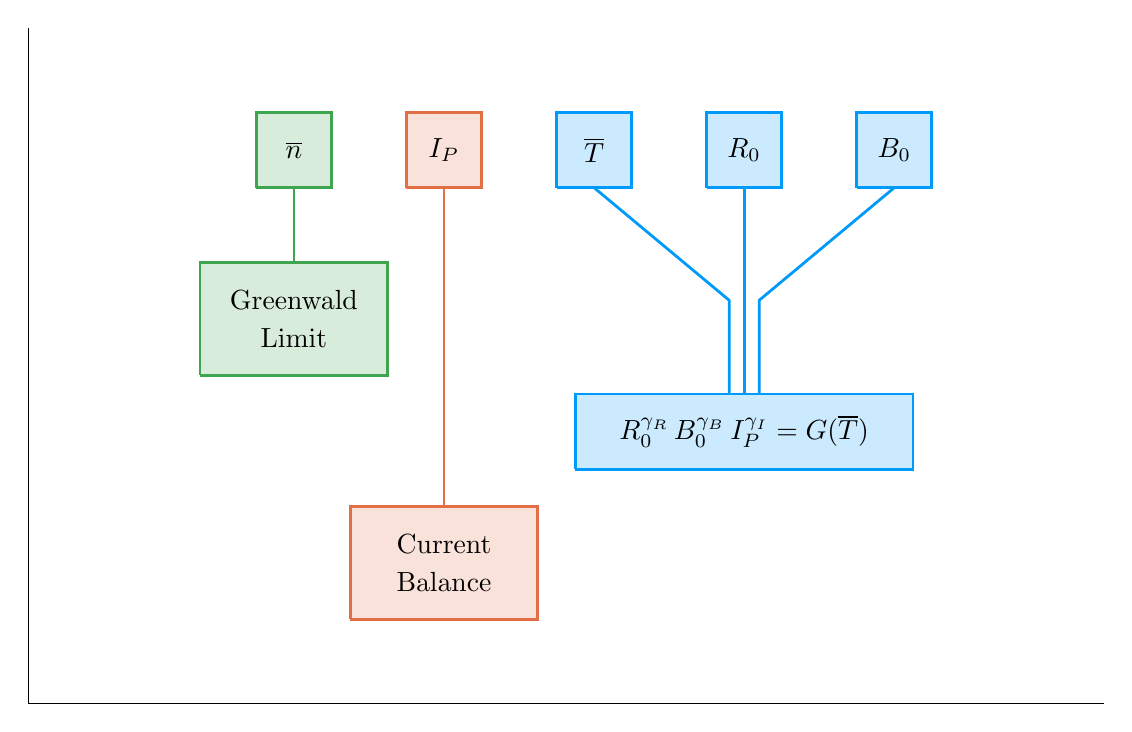
\begin{tikzpicture}[]
\begin{axis}[height = {101.6mm}, axis equal = {true}, ylabel = {}, xmin = {0.25}, xmax = {10.0}, ymax = {9.125}, xlabel = {}, {unbounded coords=jump, scaled x ticks = false, xticklabel style={rotate = 0}, xmajorticks=false, xmajorgrids = false, axis lines* = left, scaled y ticks = false, yticklabel style={rotate = 0}, ymajorticks=false, ymajorgrids = false, axis lines* = left,     xshift = 0.0mm,
    yshift = 0.0mm,
    axis background/.style={fill={rgb,1:red,1.00000000;green,1.00000000;blue,1.00000000}}
, colorbar style={title=}}, ymin = {0.125}, width = {152.4mm}]\addplot+ [color = {rgb,1:red,0.24222430;green,0.64327509;blue,0.30444865},
draw opacity=1.0,
line width=1,
solid,mark = none,
mark size = 2.0,
mark options = {
    color = {rgb,1:red,0.00000000;green,0.00000000;blue,0.00000000}, draw opacity = 1.0,
    fill = {rgb,1:red,0.24222430;green,0.64327509;blue,0.30444865}, fill opacity = 1.0,
    line width = 1,
    rotate = 0,
    solid
},fill = {rgb,1:red,0.24222430;green,0.64327509;blue,0.30444865}, fill opacity=0.2,forget plot]coordinates {
(1, 7)
(2, 7)
(2, 8)
(1, 8)
(1, 7)
};
\addplot+ [color = {rgb,1:red,0.88887350;green,0.43564919;blue,0.27812294},
draw opacity=1.0,
line width=1,
solid,mark = none,
mark size = 2.0,
mark options = {
    color = {rgb,1:red,0.00000000;green,0.00000000;blue,0.00000000}, draw opacity = 1.0,
    fill = {rgb,1:red,0.88887350;green,0.43564919;blue,0.27812294}, fill opacity = 1.0,
    line width = 1,
    rotate = 0,
    solid
},fill = {rgb,1:red,0.88887350;green,0.43564919;blue,0.27812294}, fill opacity=0.2,forget plot]coordinates {
(3, 7)
(4, 7)
(4, 8)
(3, 8)
(3, 7)
};
\addplot+ [color = {rgb,1:red,0.00000000;green,0.60560316;blue,0.97868012},
draw opacity=1.0,
line width=1,
solid,mark = none,
mark size = 2.0,
mark options = {
    color = {rgb,1:red,0.00000000;green,0.00000000;blue,0.00000000}, draw opacity = 1.0,
    fill = {rgb,1:red,0.00000000;green,0.60560316;blue,0.97868012}, fill opacity = 1.0,
    line width = 1,
    rotate = 0,
    solid
},fill = {rgb,1:red,0.00000000;green,0.60560316;blue,0.97868012}, fill opacity=0.2,forget plot]coordinates {
(5, 7)
(6, 7)
(6, 8)
(5, 8)
(5, 7)
};
\addplot+ [color = {rgb,1:red,0.00000000;green,0.60560316;blue,0.97868012},
draw opacity=1.0,
line width=1,
solid,mark = none,
mark size = 2.0,
mark options = {
    color = {rgb,1:red,0.00000000;green,0.00000000;blue,0.00000000}, draw opacity = 1.0,
    fill = {rgb,1:red,0.00000000;green,0.60560316;blue,0.97868012}, fill opacity = 1.0,
    line width = 1,
    rotate = 0,
    solid
},fill = {rgb,1:red,0.00000000;green,0.60560316;blue,0.97868012}, fill opacity=0.2,forget plot]coordinates {
(7, 7)
(8, 7)
(8, 8)
(7, 8)
(7, 7)
};
\addplot+ [color = {rgb,1:red,0.00000000;green,0.60560316;blue,0.97868012},
draw opacity=1.0,
line width=1,
solid,mark = none,
mark size = 2.0,
mark options = {
    color = {rgb,1:red,0.00000000;green,0.00000000;blue,0.00000000}, draw opacity = 1.0,
    fill = {rgb,1:red,0.00000000;green,0.60560316;blue,0.97868012}, fill opacity = 1.0,
    line width = 1,
    rotate = 0,
    solid
},fill = {rgb,1:red,0.00000000;green,0.60560316;blue,0.97868012}, fill opacity=0.2,forget plot]coordinates {
(9, 7)
(10, 7)
(10, 8)
(9, 8)
(9, 7)
};
\addplot+ [color = {rgb,1:red,0.24222430;green,0.64327509;blue,0.30444865},
draw opacity=1.0,
line width=1,
solid,mark = none,
mark size = 2.0,
mark options = {
    color = {rgb,1:red,0.00000000;green,0.00000000;blue,0.00000000}, draw opacity = 1.0,
    fill = {rgb,1:red,0.24222430;green,0.64327509;blue,0.30444865}, fill opacity = 1.0,
    line width = 1,
    rotate = 0,
    solid
},fill = {rgb,1:red,0.24222430;green,0.64327509;blue,0.30444865}, fill opacity=0.2,forget plot]coordinates {
(0.25, 4.5)
(2.75, 4.5)
(2.75, 6.0)
(0.25, 6.0)
(0.25, 4.5)
};
\addplot+ [color = {rgb,1:red,0.88887350;green,0.43564919;blue,0.27812294},
draw opacity=1.0,
line width=1,
solid,mark = none,
mark size = 2.0,
mark options = {
    color = {rgb,1:red,0.00000000;green,0.00000000;blue,0.00000000}, draw opacity = 1.0,
    fill = {rgb,1:red,0.88887350;green,0.43564919;blue,0.27812294}, fill opacity = 1.0,
    line width = 1,
    rotate = 0,
    solid
},fill = {rgb,1:red,0.88887350;green,0.43564919;blue,0.27812294}, fill opacity=0.2,forget plot]coordinates {
(2.25, 1.25)
(4.75, 1.25)
(4.75, 2.75)
(2.25, 2.75)
(2.25, 1.25)
};
\addplot+ [color = {rgb,1:red,0.00000000;green,0.60560316;blue,0.97868012},
draw opacity=1.0,
line width=1,
solid,mark = none,
mark size = 2.0,
mark options = {
    color = {rgb,1:red,0.00000000;green,0.00000000;blue,0.00000000}, draw opacity = 1.0,
    fill = {rgb,1:red,0.00000000;green,0.60560316;blue,0.97868012}, fill opacity = 1.0,
    line width = 1,
    rotate = 0,
    solid
},fill = {rgb,1:red,0.00000000;green,0.60560316;blue,0.97868012}, fill opacity=0.2,forget plot]coordinates {
(5.25, 3.25)
(9.75, 3.25)
(9.75, 4.25)
(5.25, 4.25)
(5.25, 3.25)
};
\addplot+ [color = {rgb,1:red,0.24222430;green,0.64327509;blue,0.30444865},
draw opacity=1.0,
line width=1,
solid,mark = none,
mark size = 2.0,
mark options = {
    color = {rgb,1:red,0.00000000;green,0.00000000;blue,0.00000000}, draw opacity = 1.0,
    fill = {rgb,1:red,0.24222430;green,0.64327509;blue,0.30444865}, fill opacity = 1.0,
    line width = 1,
    rotate = 0,
    solid
},forget plot]coordinates {
(1.5, 6.0)
(1.5, 7.0)
};
\addplot+ [color = {rgb,1:red,0.88887350;green,0.43564919;blue,0.27812294},
draw opacity=1.0,
line width=1,
solid,mark = none,
mark size = 2.0,
mark options = {
    color = {rgb,1:red,0.00000000;green,0.00000000;blue,0.00000000}, draw opacity = 1.0,
    fill = {rgb,1:red,0.88887350;green,0.43564919;blue,0.27812294}, fill opacity = 1.0,
    line width = 1,
    rotate = 0,
    solid
},forget plot]coordinates {
(3.5, 2.75)
(3.5, 7.0)
};
\addplot+ [color = {rgb,1:red,0.00000000;green,0.60560316;blue,0.97868012},
draw opacity=1.0,
line width=1,
solid,mark = none,
mark size = 2.0,
mark options = {
    color = {rgb,1:red,0.00000000;green,0.00000000;blue,0.00000000}, draw opacity = 1.0,
    fill = {rgb,1:red,0.00000000;green,0.60560316;blue,0.97868012}, fill opacity = 1.0,
    line width = 1,
    rotate = 0,
    solid
},forget plot]coordinates {
(5.5, 7.0)
(7.3, 5.5)
(7.3, 4.25)
};
\addplot+ [color = {rgb,1:red,0.00000000;green,0.60560316;blue,0.97868012},
draw opacity=1.0,
line width=1,
solid,mark = none,
mark size = 2.0,
mark options = {
    color = {rgb,1:red,0.00000000;green,0.00000000;blue,0.00000000}, draw opacity = 1.0,
    fill = {rgb,1:red,0.00000000;green,0.60560316;blue,0.97868012}, fill opacity = 1.0,
    line width = 1,
    rotate = 0,
    solid
},forget plot]coordinates {
(7.5, 7.0)
(7.5, 4.25)
};
\addplot+ [color = {rgb,1:red,0.00000000;green,0.60560316;blue,0.97868012},
draw opacity=1.0,
line width=1,
solid,mark = none,
mark size = 2.0,
mark options = {
    color = {rgb,1:red,0.00000000;green,0.00000000;blue,0.00000000}, draw opacity = 1.0,
    fill = {rgb,1:red,0.00000000;green,0.60560316;blue,0.97868012}, fill opacity = 1.0,
    line width = 1,
    rotate = 0,
    solid
},forget plot]coordinates {
(9.5, 7.0)
(7.7, 5.5)
(7.7, 4.25)
};
\node at (axis cs:1.5, 7.5) [,
color={rgb,1:red,0.00000000;green,0.00000000;blue,0.00000000}, draw opacity=1.0,
rotate=0.0
] {$\overline n$};
\node at (axis cs:3.5, 7.5) [,
color={rgb,1:red,0.00000000;green,0.00000000;blue,0.00000000}, draw opacity=1.0,
rotate=0.0
] {$I_P$};
\node at (axis cs:5.5, 7.5) [,
color={rgb,1:red,0.00000000;green,0.00000000;blue,0.00000000}, draw opacity=1.0,
rotate=0.0
] {$\overline T$};
\node at (axis cs:7.5, 7.5) [,
color={rgb,1:red,0.00000000;green,0.00000000;blue,0.00000000}, draw opacity=1.0,
rotate=0.0
] {$R_0$};
\node at (axis cs:9.5, 7.5) [,
color={rgb,1:red,0.00000000;green,0.00000000;blue,0.00000000}, draw opacity=1.0,
rotate=0.0
] {$B_0$};
\node at (axis cs:1.5, 5.5) [,
color={rgb,1:red,0.00000000;green,0.00000000;blue,0.00000000}, draw opacity=1.0,
rotate=0.0
] {Greenwald};
\node at (axis cs:1.5, 5) [,
color={rgb,1:red,0.00000000;green,0.00000000;blue,0.00000000}, draw opacity=1.0,
rotate=0.0
] {Limit};
\node at (axis cs:3.5, 2.25) [,
color={rgb,1:red,0.00000000;green,0.00000000;blue,0.00000000}, draw opacity=1.0,
rotate=0.0
] {Current};
\node at (axis cs:3.5, 1.75) [,
color={rgb,1:red,0.00000000;green,0.00000000;blue,0.00000000}, draw opacity=1.0,
rotate=0.0
] {Balance};
\node at (axis cs:7.5, 3.75) [,
color={rgb,1:red,0.00000000;green,0.00000000;blue,0.00000000}, draw opacity=1.0,
rotate=0.0
] {$R_0^{\gamma_R} \, B_0^{\gamma_B} \, I_P^{\gamma_I} = G(\overline T)$};
\end{axis}

\end{tikzpicture}

	\end{adjustbox}
%	\includegraphics[width=0.75\textwidth]{images/test_image}
	\caption{Equation Selection for Fusion System} ~\\
	\small The goal of this fusion system is to create a set of equations that model the five dynamic variables. These are the Greenwald limit for density, current balance for the plasma current, and three generalized formulas for the temperature, major radius, and toroidal field strength.	
	\label{fig:equation_breakdown}
\end{figure}

The logical place to start in a discussion of this algebra problem is with the three equations fundamental to all reactor-grade tokamaks -- both in steady-state and pulsed operation. These are: the Greenwald density limit, power balance, and current balance. The Greenwald density's importance was hinted early on when it was used to simplify every equation derived thereafter. 
\begin{equation}
	\tag{\ref{eq:greenwald}}
	\overline n = K_n \cdot \frac{I_P}{R_0^2}
\end{equation}
The two balance equations \replaced{proved to be}{prove} slightly more \replaced{complicated.}{dubious.} As was \replaced{shown,}{shown previously,} current balance \deleted{-- the stability requirement for tokamaks --} was \replaced{the more difficult of the two -- bringing}{most peculiar. It brought} forth the notion of self-consistency for steady-state machines and a highly-coupled multi-root equation for pulsed ones. As such, \replaced{current balance}{this equation} stands as the \replaced{equation}{one} everything \replaced{is substituted}{else will be substituted} into to \replaced{do a final}{setup for a} univariate root solve.
\begin{equation}
	\tag{\ref{eq:gen_ip}}
	I_P = \frac{ \left( K_{BS} + \sfrac{ G_{IU} }{ G_{IP} } \right) \cdot \overline T }{ 1 - K_{CD} ( \sigma v ) - \sfrac{ G_{ID} }{ G_{IP} } }
\end{equation}
Although slightly buried in \cref{eq:gen_ip}, the right-hand side actually depends on all the quantities (including $I_P$ through the \added{wall loading term in} blanket thickness). Through equation,
\begin{equation}
	I_P = f(I_P, \overline T, R_0, B_0)
\end{equation}
The remaining equation common to all reactor-grade tokamaks is power balance -- the relation that \replaced{quantifies its net electricity production capabilities.}{separates power plants from toasters.} Due to the use of the ELMy H-Mode scaling law for modeling the diffusion coefficient, this had the complicated form of:
\begin{equation}
	\label{eq:freidberg}
	R_0^{ \alpha_R^* } \cdot B_0^{\,\alpha_B} \cdot I_P^{\,\alpha_I^*} = \frac{ G_{PB} }{ K_{PB} }
\end{equation}
Although being rather cumbersome, this equation actually remains relatively simple in that all three quantities on the left-hand side are separable. To close the system, two more equations of this form are needed. These have the following form and will be described next.
\begin{equation}
	\label{eq:rbi}
	R_0^{\, \gamma_R} \cdot B_0^{\, \gamma_B} \cdot I_P^{\, \gamma_I} = G( \overline T )
\end{equation}

\section{Generalizing Previous Equations}

Where the equations defined up to this point in the chapter are shared among all fusion reactors, the remaining two equations -- needed to close the system -- must be \added{partially} chosen by the user. These \deleted{user-supplied} equations come in three \replaced{varieties:}{flavors:} limits, \replaced{intermediate}{derived} quantities, and \replaced{dynamic}{floating} variables. By convention, we enforce that at least one limit must be used. The other constraint can then come from any of the three defined collections, which we will refer to as the closure equation.

\begin{table}[hb!]
\caption[Main Equation Bank]{Main Equation Bank \\ \small To close the system of equations for potential reactors, different equations can be used to lock down tokamak designs. These include physics and engineering limits (L), as well as ways to set \replaced{dynamic (D)}{floating (F)} or \replaced{intermediate (I)}{derived (D)} variables to constant values.}
\begin{spacing}{1.5}
\begin{tabular}{lccccc}
 Variable & Category & G($\overline T$)  & $\gamma_R$ & $\gamma_B$ & $\gamma_{I}$ \\ \hline
Power Balance & - & $\sfrac{ G_{PB} }{ K_{PB} }$ & $\alpha_R^*$ & $\alpha_B$ & $\alpha_I^*$ \\
Beta ($\beta_N$) & L & $K_{TB} \overline T$ & 1 & 1 & 0 \\
Kink ($q_{\replaced{*}{95}}$) & L & $K_{KF} $ & 1 & 1 & -1 \\
Wall Loading ($P_W$) & L & $K_{WL} ( \sigma v )^{\sfrac{1}{3}} $ & 1 & 0 & -$\sfrac{2}{3}$ \\
Power Cap ($P_E$) & L & $K_{PC} ( \sigma v ) $ & 1 & 0 & -2 \\
Heat Loading ($q_{DV}$) & L & $K_{DV} ( \sigma v )^{\sfrac{1}{3.2}} $ & 1 & 0 & -1 \\
Major Radius ($R_0$) & D & $(R_0)_{const}$ & 1 & 0 & 0 \\
Magnet Strength ($B_0$) & D & $(B_0)_{const}$ & 0 & 1 & 0 \\
Plasma Current ($I_P$) & D & $(I_P)_{const}$ & 0 & 0 & 1 \\
Plasma Temperature ($\overline T$) & D & $\sfrac{ (\overline T)_{const} }{ \, \overline T }$ & 0 & 0 & 0 \\
Electron Density ($\overline n$) & D & $\sfrac{ (\overline n)_{const} }{ K_n }$ & -2 & 0 & 1 \\
Plasma Pressure ($\overline p$) & I & $\sfrac{ (\overline p)_{const} }{ K_n K_{nT} \overline T }$ & -2 & 0 & 1 
\\
Bootstrap Current ($f_{BS}$) & I & $\sfrac{ ( f_{BS} )_{const} }{ K_{BS} \overline T }$ & 0 & 0 & -1 \\
Fusion Power ($P_F$) & I & $\sfrac{ (P_F)_{const} }{ K_F K_n ^ 2 ( \sigma v ) }$ & -1 & 0 & 2 \\
Magnetic Energy ($W_M$) & I & $\sfrac{ (W_M)_{const} }{ K_{WM} }$ & 3 & 2 & 0 \\
Cost-per-Watt ($C_W$) & I & $ (C_W)_{const} \cdot \left( \sfrac{ K_F K_n ^ 2 ( \sigma v ) }{ K_{WM} } \right)$ & 4 & 2 & -2 \\
\end{tabular}
\end{spacing}
\label{table:eq}
\end{table}

\subsection{\replaced{Including Limiting Constraints}{Rehashing the Limits}}

The limits category is \replaced{composed of the limiting constraints given in \cref{chapter:model}.}{simply a rebranding of the secondary constraints given previously.} These include the physics derived limits from MHD theory -- i.e.\ the beta limit ($\beta_N$) and the kink safety factor ($q_{\replaced{*}{95}}$) -- which for clarity, set maximums on the allowed plasma pressure and \replaced{current,}{velocity,} respectively. Additionally, there were several engineering limits also described: wall loading, heat loading, and maximum power capacity. For this paper, wall loading from neutrons ($P_W$) is assumed to be important, whereas the other two engineering limits are not allowed to explicitly guide designs.

Combined all these limits, as well as the yet to be defined \replaced{dynamic}{float} and \replaced{intermediate}{derived} equations, are given in \cref{table:eq}. These share a remarkably similar form to power balance when put into a generalized, separable state. This hints at why the major radius ($R_0$), the toroidal field strength ($B_0$), and the plasma current ($I_P$) can easily be separated and substituted out of the current balance equation.

Before moving on, it proves useful to explain the two limits not used to explicitly guide reactor design -- divertor heat loading and the maximum power capacity. The simpler of the two to reason is the heat loading limit. Although removing the gigawatts\added{-per-square-meter} of heat is extremely difficult, it remains an unsolved problem worthy of its own research \replaced{machine.\cite{adx} }{machine, but currently neglected financially.} As such, it is only kept to provide a human-interpreted  measure of difficulty. The power cap, on the other hand, is just handled informally. If a reactor surpasses it (i.e.\ $ P_E > 4000 MW $), it is considered invalid.

While the maximum power cap informally sets a maximum major radius for a machine, there also exists an implicit minimum major radius. This minimum occurs due to the hole-size constraint -- i.e.\ at some point there is no longer enough room on the inside of the machine to store the central solenoid, blanket, and TF coils.

At this point, we can now explain how various quantities in the systems model can be set to user-given constant values. This basically allows users to treat one \replaced{dynamic}{floating} variable as a \replaced{static}{fixed} one (e.g.\ the temperature and bootstrap fraction).

\subsection{Minimizing \replaced{Intermediate}{Derived} Quantities} 

Whereas the limits from the previous section represented constraints with real physics and engineering repercussions, the \replaced{intermediate}{derived} quantities here are just used to find when reactors reach certain user-supplied values. Most notable are the capital cost (through the magnetic energy -- $W_M$) and the cost-per-watt ($C_W$). The model also, however, allows easily setting values for the bootstrap fraction, plasma pressure, and fusion power. As mentioned previously, they are given in \cref{table:eq} through a generalized representation of the form:
\begin{equation}
	\tag{\ref{eq:rbi}}
	R_0^{\, \gamma_R} \cdot B_0^{\, \gamma_B} \cdot I_P^{\, \gamma_I} = G( \overline T )
\end{equation}
What this collection of variables is really useful for, though, is finding minimum cost reactors -- both in a capital context as well as a cost-per-watt one. \replaced{This}{Without boring the reader, this} is done in a three stage process. \replaced{The first of which is to find a valid reactor -- i.e.\ one that satisfies every limiting constraint. Practically, this is done by searching over a range of scanned temperatures.}{First, some valid reactor is found: it does not matter if it is good, just valid. This of course can be found by systematically throwing darts at a dart board -- see \cref{fig:step_one}.}

%\begin{figure}[h]
%\centering
%\begin{adjustbox}{width=0.8\textwidth}
%	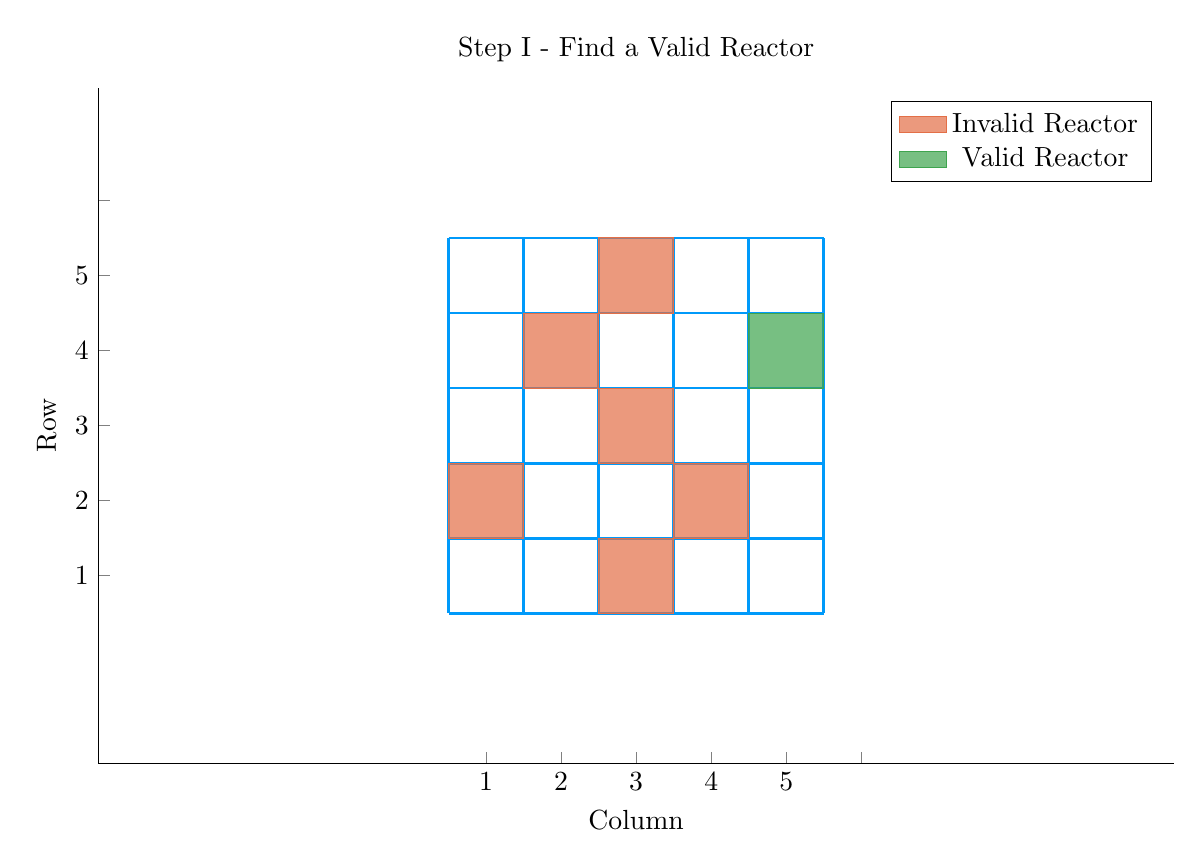
\begin{tikzpicture}[]
\begin{axis}[height = {101.6mm}, axis equal = {true}, ylabel = {Row}, title = {Step I - Find a Valid Reactor}, xmin = {0.0}, xmax = {5.0}, ymax = {7}, xlabel = {Column}, {unbounded coords=jump, xticklabel style={rotate = 0}, xmajorgrids = false, xtick = {0.5,1.5,2.5,3.5,4.5,5.5}, xticklabels = {1,2,3,4,5}, xtick align = inside, axis lines* = left, yticklabel style={rotate = 0}, ymajorgrids = false, ytick = {0.5,1.5,2.5,3.5,4.5,5.5}, yticklabels = {1,2,3,4,5}, ytick align = inside, axis lines* = left,     xshift = 0.0mm,
    yshift = 0.0mm,
    axis background/.style={fill={rgb,1:red,1.00000000;green,1.00000000;blue,1.00000000}}
}, ymin = {-2}, width = {152.4mm}]\addplot+ [color = {rgb,1:red,0.00000000;green,0.60560316;blue,0.97868012},
draw opacity=1.0,
line width=1,
solid,mark = none,
mark size = 2.0,
mark options = {
    color = {rgb,1:red,0.00000000;green,0.00000000;blue,0.00000000}, draw opacity = 1.0,
    fill = {rgb,1:red,0.00000000;green,0.60560316;blue,0.97868012}, fill opacity = 1.0,
    line width = 1,
    rotate = 0,
    solid
},forget plot]coordinates {
(0, 0)
(0, 5)
};
\addplot+ [color = {rgb,1:red,0.00000000;green,0.60560316;blue,0.97868012},
draw opacity=1.0,
line width=1,
solid,mark = none,
mark size = 2.0,
mark options = {
    color = {rgb,1:red,0.00000000;green,0.00000000;blue,0.00000000}, draw opacity = 1.0,
    fill = {rgb,1:red,0.00000000;green,0.60560316;blue,0.97868012}, fill opacity = 1.0,
    line width = 1,
    rotate = 0,
    solid
},forget plot]coordinates {
(0, 0)
(5, 0)
};
\addplot+ [color = {rgb,1:red,0.00000000;green,0.60560316;blue,0.97868012},
draw opacity=1.0,
line width=1,
solid,mark = none,
mark size = 2.0,
mark options = {
    color = {rgb,1:red,0.00000000;green,0.00000000;blue,0.00000000}, draw opacity = 1.0,
    fill = {rgb,1:red,0.00000000;green,0.60560316;blue,0.97868012}, fill opacity = 1.0,
    line width = 1,
    rotate = 0,
    solid
},forget plot]coordinates {
(1, 0)
(1, 5)
};
\addplot+ [color = {rgb,1:red,0.00000000;green,0.60560316;blue,0.97868012},
draw opacity=1.0,
line width=1,
solid,mark = none,
mark size = 2.0,
mark options = {
    color = {rgb,1:red,0.00000000;green,0.00000000;blue,0.00000000}, draw opacity = 1.0,
    fill = {rgb,1:red,0.00000000;green,0.60560316;blue,0.97868012}, fill opacity = 1.0,
    line width = 1,
    rotate = 0,
    solid
},forget plot]coordinates {
(0, 1)
(5, 1)
};
\addplot+ [color = {rgb,1:red,0.00000000;green,0.60560316;blue,0.97868012},
draw opacity=1.0,
line width=1,
solid,mark = none,
mark size = 2.0,
mark options = {
    color = {rgb,1:red,0.00000000;green,0.00000000;blue,0.00000000}, draw opacity = 1.0,
    fill = {rgb,1:red,0.00000000;green,0.60560316;blue,0.97868012}, fill opacity = 1.0,
    line width = 1,
    rotate = 0,
    solid
},forget plot]coordinates {
(2, 0)
(2, 5)
};
\addplot+ [color = {rgb,1:red,0.00000000;green,0.60560316;blue,0.97868012},
draw opacity=1.0,
line width=1,
solid,mark = none,
mark size = 2.0,
mark options = {
    color = {rgb,1:red,0.00000000;green,0.00000000;blue,0.00000000}, draw opacity = 1.0,
    fill = {rgb,1:red,0.00000000;green,0.60560316;blue,0.97868012}, fill opacity = 1.0,
    line width = 1,
    rotate = 0,
    solid
},forget plot]coordinates {
(0, 2)
(5, 2)
};
\addplot+ [color = {rgb,1:red,0.00000000;green,0.60560316;blue,0.97868012},
draw opacity=1.0,
line width=1,
solid,mark = none,
mark size = 2.0,
mark options = {
    color = {rgb,1:red,0.00000000;green,0.00000000;blue,0.00000000}, draw opacity = 1.0,
    fill = {rgb,1:red,0.00000000;green,0.60560316;blue,0.97868012}, fill opacity = 1.0,
    line width = 1,
    rotate = 0,
    solid
},forget plot]coordinates {
(3, 0)
(3, 5)
};
\addplot+ [color = {rgb,1:red,0.00000000;green,0.60560316;blue,0.97868012},
draw opacity=1.0,
line width=1,
solid,mark = none,
mark size = 2.0,
mark options = {
    color = {rgb,1:red,0.00000000;green,0.00000000;blue,0.00000000}, draw opacity = 1.0,
    fill = {rgb,1:red,0.00000000;green,0.60560316;blue,0.97868012}, fill opacity = 1.0,
    line width = 1,
    rotate = 0,
    solid
},forget plot]coordinates {
(0, 3)
(5, 3)
};
\addplot+ [color = {rgb,1:red,0.00000000;green,0.60560316;blue,0.97868012},
draw opacity=1.0,
line width=1,
solid,mark = none,
mark size = 2.0,
mark options = {
    color = {rgb,1:red,0.00000000;green,0.00000000;blue,0.00000000}, draw opacity = 1.0,
    fill = {rgb,1:red,0.00000000;green,0.60560316;blue,0.97868012}, fill opacity = 1.0,
    line width = 1,
    rotate = 0,
    solid
},forget plot]coordinates {
(4, 0)
(4, 5)
};
\addplot+ [color = {rgb,1:red,0.00000000;green,0.60560316;blue,0.97868012},
draw opacity=1.0,
line width=1,
solid,mark = none,
mark size = 2.0,
mark options = {
    color = {rgb,1:red,0.00000000;green,0.00000000;blue,0.00000000}, draw opacity = 1.0,
    fill = {rgb,1:red,0.00000000;green,0.60560316;blue,0.97868012}, fill opacity = 1.0,
    line width = 1,
    rotate = 0,
    solid
},forget plot]coordinates {
(0, 4)
(5, 4)
};
\addplot+ [color = {rgb,1:red,0.00000000;green,0.60560316;blue,0.97868012},
draw opacity=1.0,
line width=1,
solid,mark = none,
mark size = 2.0,
mark options = {
    color = {rgb,1:red,0.00000000;green,0.00000000;blue,0.00000000}, draw opacity = 1.0,
    fill = {rgb,1:red,0.00000000;green,0.60560316;blue,0.97868012}, fill opacity = 1.0,
    line width = 1,
    rotate = 0,
    solid
},forget plot]coordinates {
(5, 0)
(5, 5)
};
\addplot+ [color = {rgb,1:red,0.00000000;green,0.60560316;blue,0.97868012},
draw opacity=1.0,
line width=1,
solid,mark = none,
mark size = 2.0,
mark options = {
    color = {rgb,1:red,0.00000000;green,0.00000000;blue,0.00000000}, draw opacity = 1.0,
    fill = {rgb,1:red,0.00000000;green,0.60560316;blue,0.97868012}, fill opacity = 1.0,
    line width = 1,
    rotate = 0,
    solid
},forget plot]coordinates {
(0, 5)
(5, 5)
};
\addplot+ [color = {rgb,1:red,0.88887350;green,0.43564919;blue,0.27812294},
draw opacity=1.0,
line width=0,
solid,mark = none,
mark size = 2.0,
mark options = {
    color = {rgb,1:red,0.00000000;green,0.00000000;blue,0.00000000}, draw opacity = 1.0,
    fill = {rgb,1:red,0.88887350;green,0.43564919;blue,0.27812294}, fill opacity = 1.0,
    line width = 1,
    rotate = 0,
    solid
},fill = {rgb,1:red,0.88887350;green,0.43564919;blue,0.27812294}, fill opacity=0.7,area legend]coordinates {
(2, 2)
(2, 3)
(3, 3)
(3, 2)
(2, 2)
};
\addlegendentry{Invalid Reactor}
\addplot+ [color = {rgb,1:red,0.88887350;green,0.43564919;blue,0.27812294},
draw opacity=1.0,
line width=0,
solid,mark = none,
mark size = 2.0,
mark options = {
    color = {rgb,1:red,0.00000000;green,0.00000000;blue,0.00000000}, draw opacity = 1.0,
    fill = {rgb,1:red,0.88887350;green,0.43564919;blue,0.27812294}, fill opacity = 1.0,
    line width = 1,
    rotate = 0,
    solid
},fill = {rgb,1:red,0.88887350;green,0.43564919;blue,0.27812294}, fill opacity=0.7,forget plot]coordinates {
(1, 3)
(1, 4)
(2, 4)
(2, 3)
(1, 3)
};
\addplot+ [color = {rgb,1:red,0.88887350;green,0.43564919;blue,0.27812294},
draw opacity=1.0,
line width=0,
solid,mark = none,
mark size = 2.0,
mark options = {
    color = {rgb,1:red,0.00000000;green,0.00000000;blue,0.00000000}, draw opacity = 1.0,
    fill = {rgb,1:red,0.88887350;green,0.43564919;blue,0.27812294}, fill opacity = 1.0,
    line width = 1,
    rotate = 0,
    solid
},fill = {rgb,1:red,0.88887350;green,0.43564919;blue,0.27812294}, fill opacity=0.7,forget plot]coordinates {
(3, 1)
(3, 2)
(4, 2)
(4, 1)
(3, 1)
};
\addplot+ [color = {rgb,1:red,0.88887350;green,0.43564919;blue,0.27812294},
draw opacity=1.0,
line width=0,
solid,mark = none,
mark size = 2.0,
mark options = {
    color = {rgb,1:red,0.00000000;green,0.00000000;blue,0.00000000}, draw opacity = 1.0,
    fill = {rgb,1:red,0.88887350;green,0.43564919;blue,0.27812294}, fill opacity = 1.0,
    line width = 1,
    rotate = 0,
    solid
},fill = {rgb,1:red,0.88887350;green,0.43564919;blue,0.27812294}, fill opacity=0.7,forget plot]coordinates {
(2, 4)
(2, 5)
(3, 5)
(3, 4)
(2, 4)
};
\addplot+ [color = {rgb,1:red,0.88887350;green,0.43564919;blue,0.27812294},
draw opacity=1.0,
line width=0,
solid,mark = none,
mark size = 2.0,
mark options = {
    color = {rgb,1:red,0.00000000;green,0.00000000;blue,0.00000000}, draw opacity = 1.0,
    fill = {rgb,1:red,0.88887350;green,0.43564919;blue,0.27812294}, fill opacity = 1.0,
    line width = 1,
    rotate = 0,
    solid
},fill = {rgb,1:red,0.88887350;green,0.43564919;blue,0.27812294}, fill opacity=0.7,forget plot]coordinates {
(0, 1)
(0, 2)
(1, 2)
(1, 1)
(0, 1)
};
\addplot+ [color = {rgb,1:red,0.88887350;green,0.43564919;blue,0.27812294},
draw opacity=1.0,
line width=0,
solid,mark = none,
mark size = 2.0,
mark options = {
    color = {rgb,1:red,0.00000000;green,0.00000000;blue,0.00000000}, draw opacity = 1.0,
    fill = {rgb,1:red,0.88887350;green,0.43564919;blue,0.27812294}, fill opacity = 1.0,
    line width = 1,
    rotate = 0,
    solid
},fill = {rgb,1:red,0.88887350;green,0.43564919;blue,0.27812294}, fill opacity=0.7,forget plot]coordinates {
(2, 0)
(2, 1)
(3, 1)
(3, 0)
(2, 0)
};
\addplot+ [color = {rgb,1:red,0.24222430;green,0.64327509;blue,0.30444865},
draw opacity=1.0,
line width=0,
solid,mark = none,
mark size = 2.0,
mark options = {
    color = {rgb,1:red,0.00000000;green,0.00000000;blue,0.00000000}, draw opacity = 1.0,
    fill = {rgb,1:red,0.24222430;green,0.64327509;blue,0.30444865}, fill opacity = 1.0,
    line width = 1,
    rotate = 0,
    solid
},fill = {rgb,1:red,0.24222430;green,0.64327509;blue,0.30444865}, fill opacity=0.7,area legend]coordinates {
(4, 3)
(4, 4)
(5, 4)
(5, 3)
(4, 3)
};
\addlegendentry{Valid Reactor}
\end{axis}

\end{tikzpicture}

%\end{adjustbox}
%\caption{Minimize Cost Step I -- Find Valid Reactor}
%\label{fig:step_one}
%\end{figure}

After a valid reactor is found, its cost is recorded leading to a drill-down stage. In this step, the cost is continuously halved until a valid reactor cannot be found. Once this invalid reactor is reached, it sets a bound on the minimum cost reactor. As such, the final stage is a simple bisection step where the minimum cost is honed down to some acceptable margin of error -- see \cref{fig:minimize}.

\begin{figure*}
    \centering
    \begin{subfigure}[t]{0.8\textwidth}
        \centering
		\begin{adjustbox}{width=\textwidth}
			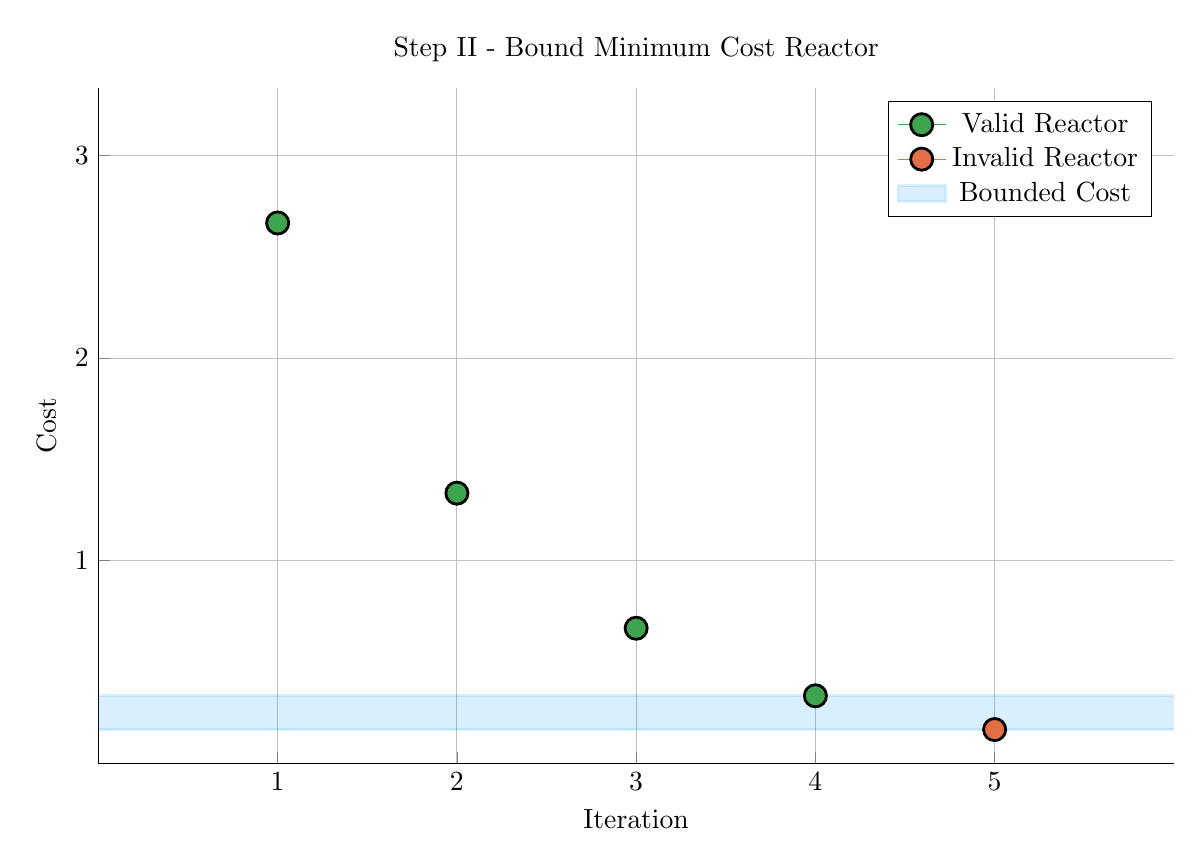
\begin{tikzpicture}[]
\begin{axis}[height = {101.6mm}, ylabel = {Cost}, title = {Step II - Bound Minimum Cost Reactor}, xmin = {0}, xmax = {6}, ymax = {40}, xlabel = {Iteration}, {unbounded coords=jump, xticklabel style={rotate = 0}, xmajorgrids = true, xtick = {1.0,2.0,3.0,4.0,5.0}, xticklabels = {1,2,3,4,5}, xtick align = inside, axis lines* = left, yticklabel style={rotate = 0}, ymajorgrids = true, ytick = {12,24,36}, yticklabels = {1,2,3}, ytick align = inside, axis lines* = left,     xshift = 0.0mm,
    yshift = 0.0mm,
    axis background/.style={fill={rgb,1:red,1.00000000;green,1.00000000;blue,1.00000000}}
}, ymin = {0}, width = {152.4mm}]\addplot+[draw=none, color = {rgb,1:red,0.24222430;green,0.64327509;blue,0.30444865},
draw opacity=1.0,
line width=0,
solid,mark = *,
mark size = 4.0,
mark options = {
    color = {rgb,1:red,0.00000000;green,0.00000000;blue,0.00000000}, draw opacity = 1.0,
    fill = {rgb,1:red,0.24222430;green,0.64327509;blue,0.30444865}, fill opacity = 1.0,
    line width = 1,
    rotate = 0,
    solid
}] coordinates {
(1.0, 32.0)
};
\addlegendentry{Valid Reactor}
\addplot+[draw=none, color = {rgb,1:red,0.24222430;green,0.64327509;blue,0.30444865},
draw opacity=1.0,
line width=0,
solid,mark = *,
mark size = 4.0,
mark options = {
    color = {rgb,1:red,0.00000000;green,0.00000000;blue,0.00000000}, draw opacity = 1.0,
    fill = {rgb,1:red,0.24222430;green,0.64327509;blue,0.30444865}, fill opacity = 1.0,
    line width = 1,
    rotate = 0,
    solid
},forget plot] coordinates {
(2.0, 16.0)
};
\addplot+[draw=none, color = {rgb,1:red,0.24222430;green,0.64327509;blue,0.30444865},
draw opacity=1.0,
line width=0,
solid,mark = *,
mark size = 4.0,
mark options = {
    color = {rgb,1:red,0.00000000;green,0.00000000;blue,0.00000000}, draw opacity = 1.0,
    fill = {rgb,1:red,0.24222430;green,0.64327509;blue,0.30444865}, fill opacity = 1.0,
    line width = 1,
    rotate = 0,
    solid
},forget plot] coordinates {
(3.0, 8.0)
};
\addplot+[draw=none, color = {rgb,1:red,0.24222430;green,0.64327509;blue,0.30444865},
draw opacity=1.0,
line width=0,
solid,mark = *,
mark size = 4.0,
mark options = {
    color = {rgb,1:red,0.00000000;green,0.00000000;blue,0.00000000}, draw opacity = 1.0,
    fill = {rgb,1:red,0.24222430;green,0.64327509;blue,0.30444865}, fill opacity = 1.0,
    line width = 1,
    rotate = 0,
    solid
},forget plot] coordinates {
(4.0, 4.0)
};
\addplot+[draw=none, color = {rgb,1:red,0.88887350;green,0.43564919;blue,0.27812294},
draw opacity=1.0,
line width=0,
solid,mark = *,
mark size = 4.0,
mark options = {
    color = {rgb,1:red,0.00000000;green,0.00000000;blue,0.00000000}, draw opacity = 1.0,
    fill = {rgb,1:red,0.88887350;green,0.43564919;blue,0.27812294}, fill opacity = 1.0,
    line width = 1,
    rotate = 0,
    solid
}] coordinates {
(5.0, 2.0)
};
\addlegendentry{Invalid Reactor}
\addplot+ [color = {rgb,1:red,0.00000000;green,0.60560316;blue,0.97868012},
draw opacity=0.15,
line width=1,
solid,mark = none,
mark size = 2.0,
mark options = {
    color = {rgb,1:red,0.00000000;green,0.00000000;blue,0.00000000}, draw opacity = 0.15,
    fill = {rgb,1:red,0.00000000;green,0.60560316;blue,0.97868012}, fill opacity = 0.15,
    line width = 1,
    rotate = 0,
    solid
},fill = {rgb,1:red,0.00000000;green,0.60560316;blue,0.97868012}, fill opacity=0.15,area legend]coordinates {
(-1.0, 4.0)
(-1.0, 2.0)
(7.0, 2.0)
(7.0, 4.0)
(-1.0, 4.0)
};
\addlegendentry{Bounded Cost}
\end{axis}

\end{tikzpicture}

		\end{adjustbox}
        \caption{ Minimize Step II }
    \end{subfigure} 
    \par \bigskip \par \bigskip 
    \begin{subfigure}[t]{0.8\textwidth}
        \centering
		\begin{adjustbox}{width=\textwidth}
			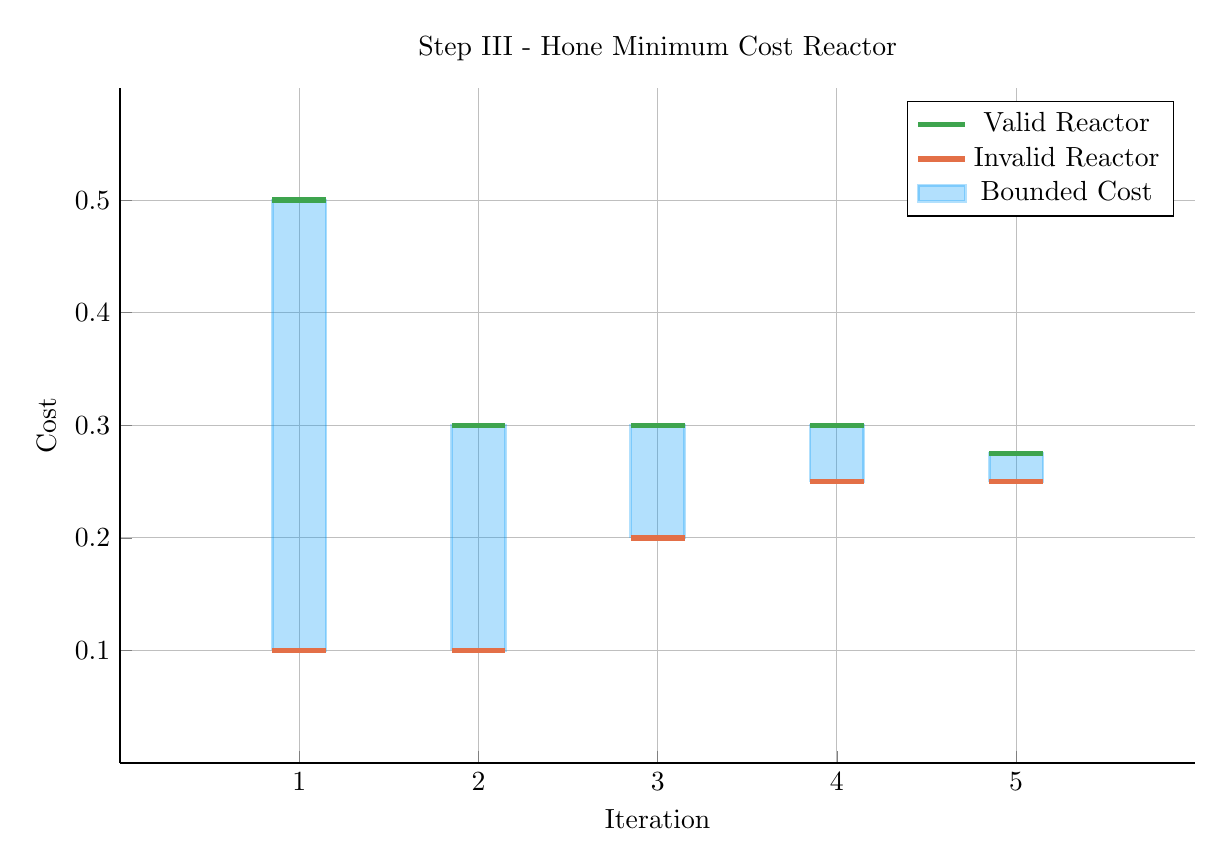
\begin{tikzpicture}[]
\begin{axis}[height = {101.6mm}, ylabel = {Cost}, title = {Step III - Hone Minimum Cost Reactor}, xmin = {0}, xmax = {6}, ymax = {0.6}, xlabel = {Iteration}, {unbounded coords=jump, xticklabel style={rotate = 0}, xmajorgrids = true, xtick = {1.0,2.0,3.0,4.0,5.0}, xticklabels = {1,2,3,4,5}, xtick align = inside, axis lines* = left, yticklabel style={rotate = 0}, ymajorgrids = true, ytick = {0.1,0.2,0.3,0.4,0.5}, yticklabels = {0.1,0.2,0.3,0.4,0.5}, ytick align = inside, axis lines* = left,     xshift = 0.0mm,
    yshift = 0.0mm,
    axis background/.style={fill={rgb,1:red,1.00000000;green,1.00000000;blue,1.00000000}}
}, ymin = {0}, width = {152.4mm}]\addplot+ [color = {rgb,1:red,0.00000000;green,0.60560316;blue,0.97868012},
draw opacity=0.3,
line width=1,
solid,mark = none,
mark size = 2.0,
mark options = {
    color = {rgb,1:red,0.00000000;green,0.00000000;blue,0.00000000}, draw opacity = 0.3,
    fill = {rgb,1:red,0.00000000;green,0.60560316;blue,0.97868012}, fill opacity = 0.3,
    line width = 1,
    rotate = 0,
    solid
},fill = {rgb,1:red,0.00000000;green,0.60560316;blue,0.97868012}, fill opacity=0.3,forget plot]coordinates {
(0.85, 0.1)
(0.85, 0.5)
(1.15, 0.5)
(1.15, 0.1)
(0.85, 0.1)
};
\addplot+ [color = {rgb,1:red,0.24222430;green,0.64327509;blue,0.30444865},
draw opacity=1.0,
line width=2,
solid,mark = none,
mark size = 2.0,
mark options = {
    color = {rgb,1:red,0.00000000;green,0.00000000;blue,0.00000000}, draw opacity = 1.0,
    fill = {rgb,1:red,0.24222430;green,0.64327509;blue,0.30444865}, fill opacity = 1.0,
    line width = 1,
    rotate = 0,
    solid
}]coordinates {
(0.85, 0.5)
(1.15, 0.5)
};
\addlegendentry{Valid Reactor}
\addplot+ [color = {rgb,1:red,0.88887350;green,0.43564919;blue,0.27812294},
draw opacity=1.0,
line width=2,
solid,mark = none,
mark size = 2.0,
mark options = {
    color = {rgb,1:red,0.00000000;green,0.00000000;blue,0.00000000}, draw opacity = 1.0,
    fill = {rgb,1:red,0.88887350;green,0.43564919;blue,0.27812294}, fill opacity = 1.0,
    line width = 1,
    rotate = 0,
    solid
}]coordinates {
(0.85, 0.1)
(1.15, 0.1)
};
\addlegendentry{Invalid Reactor}
\addplot+ [color = {rgb,1:red,0.00000000;green,0.60560316;blue,0.97868012},
draw opacity=0.3,
line width=1,
solid,mark = none,
mark size = 2.0,
mark options = {
    color = {rgb,1:red,0.00000000;green,0.00000000;blue,0.00000000}, draw opacity = 0.3,
    fill = {rgb,1:red,0.00000000;green,0.60560316;blue,0.97868012}, fill opacity = 0.3,
    line width = 1,
    rotate = 0,
    solid
},fill = {rgb,1:red,0.00000000;green,0.60560316;blue,0.97868012}, fill opacity=0.3,area legend]coordinates {
(1.85, 0.1)
(1.85, 0.3)
(2.15, 0.3)
(2.15, 0.1)
(1.85, 0.1)
};
\addlegendentry{Bounded Cost}
\addplot+ [color = {rgb,1:red,0.88887350;green,0.43564919;blue,0.27812294},
draw opacity=1.0,
line width=2,
solid,mark = none,
mark size = 2.0,
mark options = {
    color = {rgb,1:red,0.00000000;green,0.00000000;blue,0.00000000}, draw opacity = 1.0,
    fill = {rgb,1:red,0.88887350;green,0.43564919;blue,0.27812294}, fill opacity = 1.0,
    line width = 1,
    rotate = 0,
    solid
},forget plot]coordinates {
(1.85, 0.1)
(2.15, 0.1)
};
\addplot+ [color = {rgb,1:red,0.24222430;green,0.64327509;blue,0.30444865},
draw opacity=1.0,
line width=2,
solid,mark = none,
mark size = 2.0,
mark options = {
    color = {rgb,1:red,0.00000000;green,0.00000000;blue,0.00000000}, draw opacity = 1.0,
    fill = {rgb,1:red,0.24222430;green,0.64327509;blue,0.30444865}, fill opacity = 1.0,
    line width = 1,
    rotate = 0,
    solid
},forget plot]coordinates {
(1.85, 0.3)
(2.15, 0.3)
};
\addplot+ [color = {rgb,1:red,0.00000000;green,0.60560316;blue,0.97868012},
draw opacity=0.3,
line width=1,
solid,mark = none,
mark size = 2.0,
mark options = {
    color = {rgb,1:red,0.00000000;green,0.00000000;blue,0.00000000}, draw opacity = 0.3,
    fill = {rgb,1:red,0.00000000;green,0.60560316;blue,0.97868012}, fill opacity = 0.3,
    line width = 1,
    rotate = 0,
    solid
},fill = {rgb,1:red,0.00000000;green,0.60560316;blue,0.97868012}, fill opacity=0.3,forget plot]coordinates {
(2.85, 0.2)
(2.85, 0.3)
(3.15, 0.3)
(3.15, 0.2)
(2.85, 0.2)
};
\addplot+ [color = {rgb,1:red,0.88887350;green,0.43564919;blue,0.27812294},
draw opacity=1.0,
line width=2,
solid,mark = none,
mark size = 2.0,
mark options = {
    color = {rgb,1:red,0.00000000;green,0.00000000;blue,0.00000000}, draw opacity = 1.0,
    fill = {rgb,1:red,0.88887350;green,0.43564919;blue,0.27812294}, fill opacity = 1.0,
    line width = 1,
    rotate = 0,
    solid
},forget plot]coordinates {
(2.85, 0.2)
(3.15, 0.2)
};
\addplot+ [color = {rgb,1:red,0.24222430;green,0.64327509;blue,0.30444865},
draw opacity=1.0,
line width=2,
solid,mark = none,
mark size = 2.0,
mark options = {
    color = {rgb,1:red,0.00000000;green,0.00000000;blue,0.00000000}, draw opacity = 1.0,
    fill = {rgb,1:red,0.24222430;green,0.64327509;blue,0.30444865}, fill opacity = 1.0,
    line width = 1,
    rotate = 0,
    solid
},forget plot]coordinates {
(2.85, 0.3)
(3.15, 0.3)
};
\addplot+ [color = {rgb,1:red,0.00000000;green,0.60560316;blue,0.97868012},
draw opacity=0.3,
line width=1,
solid,mark = none,
mark size = 2.0,
mark options = {
    color = {rgb,1:red,0.00000000;green,0.00000000;blue,0.00000000}, draw opacity = 0.3,
    fill = {rgb,1:red,0.00000000;green,0.60560316;blue,0.97868012}, fill opacity = 0.3,
    line width = 1,
    rotate = 0,
    solid
},fill = {rgb,1:red,0.00000000;green,0.60560316;blue,0.97868012}, fill opacity=0.3,forget plot]coordinates {
(3.85, 0.25)
(3.85, 0.3)
(4.15, 0.3)
(4.15, 0.25)
(3.85, 0.25)
};
\addplot+ [color = {rgb,1:red,0.88887350;green,0.43564919;blue,0.27812294},
draw opacity=1.0,
line width=2,
solid,mark = none,
mark size = 2.0,
mark options = {
    color = {rgb,1:red,0.00000000;green,0.00000000;blue,0.00000000}, draw opacity = 1.0,
    fill = {rgb,1:red,0.88887350;green,0.43564919;blue,0.27812294}, fill opacity = 1.0,
    line width = 1,
    rotate = 0,
    solid
},forget plot]coordinates {
(3.85, 0.25)
(4.15, 0.25)
};
\addplot+ [color = {rgb,1:red,0.24222430;green,0.64327509;blue,0.30444865},
draw opacity=1.0,
line width=2,
solid,mark = none,
mark size = 2.0,
mark options = {
    color = {rgb,1:red,0.00000000;green,0.00000000;blue,0.00000000}, draw opacity = 1.0,
    fill = {rgb,1:red,0.24222430;green,0.64327509;blue,0.30444865}, fill opacity = 1.0,
    line width = 1,
    rotate = 0,
    solid
},forget plot]coordinates {
(3.85, 0.3)
(4.15, 0.3)
};
\addplot+ [color = {rgb,1:red,0.00000000;green,0.60560316;blue,0.97868012},
draw opacity=0.3,
line width=1,
solid,mark = none,
mark size = 2.0,
mark options = {
    color = {rgb,1:red,0.00000000;green,0.00000000;blue,0.00000000}, draw opacity = 0.3,
    fill = {rgb,1:red,0.00000000;green,0.60560316;blue,0.97868012}, fill opacity = 0.3,
    line width = 1,
    rotate = 0,
    solid
},fill = {rgb,1:red,0.00000000;green,0.60560316;blue,0.97868012}, fill opacity=0.3,forget plot]coordinates {
(4.85, 0.25)
(4.85, 0.275)
(5.15, 0.275)
(5.15, 0.25)
(4.85, 0.25)
};
\addplot+ [color = {rgb,1:red,0.88887350;green,0.43564919;blue,0.27812294},
draw opacity=1.0,
line width=2,
solid,mark = none,
mark size = 2.0,
mark options = {
    color = {rgb,1:red,0.00000000;green,0.00000000;blue,0.00000000}, draw opacity = 1.0,
    fill = {rgb,1:red,0.88887350;green,0.43564919;blue,0.27812294}, fill opacity = 1.0,
    line width = 1,
    rotate = 0,
    solid
},forget plot]coordinates {
(4.85, 0.25)
(5.15, 0.25)
};
\addplot+ [color = {rgb,1:red,0.24222430;green,0.64327509;blue,0.30444865},
draw opacity=1.0,
line width=2,
solid,mark = none,
mark size = 2.0,
mark options = {
    color = {rgb,1:red,0.00000000;green,0.00000000;blue,0.00000000}, draw opacity = 1.0,
    fill = {rgb,1:red,0.24222430;green,0.64327509;blue,0.30444865}, fill opacity = 1.0,
    line width = 1,
    rotate = 0,
    solid
},forget plot]coordinates {
(4.85, 0.275)
(5.15, 0.275)
};
\end{axis}

\end{tikzpicture}

		\end{adjustbox}
        \caption{ Minimize Step III }
    \end{subfigure}
    \par \bigskip \par \bigskip    
    \caption{Minimize Cost Step II/III -- Optimize Reactor}
    \label{fig:minimize} 
\end{figure*}

\subsection{Pinning \replaced{Dynamic}{Floating} Variables} 

The remaining collection of closure equations is for the five \replaced{dynamic}{floating} variables in the systems model: $R_0$, $B_0$, $\overline n$, $\overline T$, and $I_P$. As we are making equations of the following form, the formulas for $R_0$, $B_0$, and $I_P$ are trivial.
\begin{equation}
	\tag{\ref{eq:rbi}}
	R_0^{\, \gamma_R} \cdot B_0^{\, \gamma_B} \cdot I_P^{\, \gamma_I} = G( \overline T )
\end{equation}
Next, the equation for $\overline n$ -- shown in \cref{table:eq} -- is just a simple undoing of the Greenwald density limit. The remaining equation is then from the original temperature equation:
\begin{equation}
	\tag{\ref{eq:tbar}}
	\overline T = const.
\end{equation}
As was assumed earlier, this is sort of a default equation for the systems model. By this, we mean reactor curves can be created by scanning over temperatures, i.e.\ set $\overline T = 5 \ \textnormal{keV}$ in one run, 10 in the next, etc. This temperature equation also brings up a \replaced{difficulty for the algebraic solver, as it does not depend on:}{subtlety of the model, as it does not depend on} current, radius, or magnet strength. \added{Overcoming this difficulty is discussed next subsection.}

\subsection{Detailing the Equation Solver}

The algorithm that motivated this generalized equation approach most notably bifurcates in the situation where the closure equation does not depend on $R_0$, $B_0$, or $I_P$ (i.e.\ \added{for} the temperature equation). The two scenarios are given in \cref{eq:case_1_R,eq:case_1_B,eq:case_1_I,eq:case_1_gamma,eq:case_2_R,eq:case_2_B,eq:case_2_gamma} -- where at least $R_0$ and $B_0$ are substituted out of the system. In the temperature case, $I_P$ is not needed to be explicitly removed. 

Concretely, the root solve for the temperature  scenario is for the current, whereas it is for the temperature in all other cases. The nomenclature in the code is a \emph{match} for Scenario I (i.e.\ root solving for plasma temperature), and a \emph{solve} for Scenario II (i.e.\ root solving for plasma current).

\subsubsection{Scenario I -- Match for $\overline T$}

\begin{equation}
	\label{eq:case_1_R}
	R_0( \overline T) = \left( 
	G_1 ^ {  \, ( \gamma_{B,2} \, \gamma_{I,3} - \gamma_{B,3} \, \gamma_{I,2} ) } \cdot 
	G_2 ^ {  \, ( \gamma_{B,3} \, \gamma_{I,1} - \gamma_{B,1} \, \gamma_{I,3} ) } \cdot 
	G_3 ^ {  \, ( \gamma_{B,1} \, \gamma_{I,2} - \gamma_{B,2} \, \gamma_{I,1} ) }\right)^{ \frac{1}{\gamma_{RBI}} }
\end{equation}
\begin{equation}
	\label{eq:case_1_B}
	B_0( \overline T) = \left( 
	G_1 ^ {  \, ( \gamma_{I,2} \, \gamma_{R,3} - \gamma_{I,3} \, \gamma_{R,2} ) } \cdot 
	G_2 ^ {  \, ( \gamma_{I,3} \, \gamma_{R,1} - \gamma_{I,1} \, \gamma_{R,3} ) } \cdot 
	G_3 ^ {  \, ( \gamma_{I,1} \, \gamma_{R,2} - \gamma_{I,2} \, \gamma_{R,1} ) }\right)^{ \frac{1}{\gamma_{RBI}} }
\end{equation}
\begin{equation}
	\label{eq:case_1_I}
	I_P( \overline T) = \left( 
	G_1 ^ {  \, ( \gamma_{R,2} \, \gamma_{B,3} - \gamma_{R,3} \, \gamma_{B,2} ) } \cdot 
	G_2 ^ {  \, ( \gamma_{R,3} \, \gamma_{B,1} - \gamma_{R,1} \, \gamma_{B,3} ) } \cdot 
	G_3 ^ {  \, ( \gamma_{R,1} \, \gamma_{B,2} - \gamma_{R,2} \, \gamma_{B,1} ) }\right)^{ \frac{1}{\gamma_{RBI}} }
\end{equation}
\begin{gather}
	\label{eq:case_1_gamma}
	\gamma_{RBI} = ( \gamma_{R,1} \, \gamma_{B,2} \, \gamma_{I,3} +  \gamma_{R,2} \, \gamma_{B,3} \, \gamma_{I,1} + \gamma_{R,3} \, \gamma_{B,1} \, \gamma_{I,2} ) - \\
	\ \ \ \ \ \ \ \ \ \ \ \ \ \ \ ( \gamma_{R,1} \, \gamma_{B,3} \, \gamma_{I,2} +  \gamma_{R,2} \, \gamma_{B,1} \, \gamma_{I,3} + \gamma_{R,3} \, \gamma_{B,2} \, \gamma_{I,1} ) \nonumber
\end{gather}

\subsubsection{Scenario II -- Solve for $I_P$}

\begin{equation}
	\label{eq:case_2_R}
	R_0( \overline T) = \left( 
	G_1 ^ {  \, \gamma_{B,2} } \cdot 
	G_2 ^ {  \, -\gamma_{B,1} } \cdot 
	I_P ^ {  \, ( \gamma_{B,1} \, \gamma_{I,2} - \gamma_{B,2} \, \gamma_{I,1} ) }\right)^{ \frac{1}{\gamma_{RBT}} }
\end{equation}
\begin{equation}
	\label{eq:case_2_B}
	B_0( \overline T) = \left( 
	G_1 ^ {  \, -\gamma_{R,2} } \cdot 
	G_2 ^ {  \, \gamma_{R,1} } \cdot 
	I_P ^ {  \, ( \gamma_{I,1} \, \gamma_{R,2} - \gamma_{I,2} \, \gamma_{R,1} ) }\right)^{ \frac{1}{\gamma_{RBT}} }
\end{equation}
\begin{equation}
	\label{eq:case_2_gamma}
	\gamma_{RBT} = \gamma_{R,1} \, \gamma_{B,2} - \gamma_{R,2} \, \gamma_{B,1}
\end{equation}

\section{Wrapping up the Logic} 

As stated at the beginning of the chapter, this systems model basically \replaced{reduces}{boils down} to a simple 5 equation/5 unknown algebra problem. The Greenwald density was implicitly used in the initial derive to simplify the logic. The current balance was then delegated to be the root solve equation. Lastly, three equations were needed to remove the major radius and magnet strength, as well as either the current or temperature. These 16 equations were given in \cref{table:eq} with the generalized solution given in \cref{eq:case_1_R,eq:case_1_B,eq:case_1_I,eq:case_1_gamma,eq:case_2_R,eq:case_2_B,eq:case_2_gamma}.

This now sets the stage for the most interesting part of the document -- the results. \replaced{These}{In true Dickens fashion, they} will come in several forms. The first result type \deleted{we will encounter} will be temperature \replaced{scans that}{scans. These} allow us to validate the model \replaced{against other}{by comparing it to several} designs from the literature. \replaced{These are created using}{These will use} the Scenario II solver.

\replaced{The}{Moving onto examples of the} Scenario I matcher \replaced{will then be used to create}{are} sensitivity studies and Monte Carlo samplings. The simple one variable sensitivities will reveal local trends from sweeping various \replaced{static}{fixed} (i.e.\ input) variables -- namely H, $\kappa$, $B_{CS}$, etc.\ \added{-- one at a time.} Whereas the samplings will highlight global trends as many \replaced{static}{fixed}/input variables are allowed to vary simultaneously.

 These Scenario I \replaced{matchers}{flavors} are further subdivided in regards to the nature of their closure equation. The first \replaced{type}{flavor} comes from finding so called two limit solutions, which live at the point where the beta and kink (or wall) limits are just marginally satisfied. The second main type is then minimum cost reactors -- measured in either a capital cost or cost-per-watt context. These will be used in depth next chapter.
 
%\end{document}

%\documentclass[11pt]{book}
%
%\setlength{\parindent}{0pt}
%\setlength{\parskip}{8pt}
%
%\usepackage{amsmath}
%\usepackage{amssymb}
%\usepackage{hyperref}
%\usepackage{cleveref}
%
%\renewcommand*{\thefootnote}{\fnsymbol{footnote}}
%
%\setcounter{chapter}{3}
%
%\begin{document}
%
%\section*{A Levelized Comparison of \\ Pulsed and Steady-State Tokamaks}
%
%\let\cleardoublepage\relax \tableofcontents \newpage

\chapter{Presenting the Code Results}

Now that our fusion systems model has been formulated and completed, the next logical step is to \replaced{build a codebase and explore reactor space.}{code it up and run it to produce interesting data.} To this, the code \replaced{encompassing this document's model}{for this document} -- Fussy.jl -- is available at \href{http://git.io/tokamak}{git.io/tokamak} (with a short guide given in \cref{chapter:fussy}). \replaced{The results from this chapter will be divided into}{The results will be given shortly. \\
Before accosting the reader with some twenty plots and tables, though, it makes sense to first warn them what they are getting into. This chapter has} three sections. The first is an attempt to test how \replaced{accurate}{good} the model is by comparing it with other codes in the field.\cite{arc,eupulsed,process}. \replaced{The next will be two prototypes developed to fairly compare pulsed and steady state reactors, the initial motivation for this project.}{Next, we will develop two prototype reactors that pit steady-state against pulsed operation on a levelized playing field.}

This chapter will then conclude with a discussion on how best to lower \replaced{reactor costs.}{the costs of a tokamak reactor.} In line with the MIT mission, this will highlight how using stronger magnets leads to more compact, \replaced{economic}{efficient} machines. The new piece of insight, then, is how to optimally incorporate high-temperature superconducting (HTS) tape technology -- the \replaced{assumed technological advancement}{miracle} found in the ARC design family.

\replaced{Succinctly,}{Without spoiling too much for the reader,} we will show that HTS tape should be used in the TF coils for steady-state tokamaks (i.e.\ $B_0$), whereas it should only be appear in the central solenoid (i.e.\ $B_{CS}$) for pulsed ones. This is a fundamentally new result!

\section{\replaced{Testing the}{Validating} Code \replaced{against}{with} other Models}

\replaced{After developing a new model, the first next step is to make sure its results are sensical.}{When you develop a new model, the first thing you have to do is check that it makes sensical results.} The \replaced{goal, however,}{goal} is \added{to} not \deleted{to}go \replaced{too far, i.e.\ }{overboard, though,} by: comparing it with too many models or requiring perfect matches with \deleted{all}their results. To this, we will compare Fussy.jl with five designs \deleted{coming}from \replaced{the literature}{three separate research teams} -- hopefully casting a wide enough net through reactor-space to prove sufficient. It should be noted that for how simple this model is, it does a remarkable job matching \replaced{the other group's}{these} more sophisticated frameworks. It also highlights how discrepancies arise in this highly non-linear computational problem.

The first reactor design that will provide a basis for comparison is the ARC reactor.\cite{arc} As it was also designed by MIT researchers, the fit is shown to be almost exact. This of course probably involves a fair amount of inherent biases stemming from \replaced{shared scientific philosophies and knowledge base.}{how this ecosystem operates and produces engineers -- most notably as the core of this code comes from Jeff's ongoing interest in the problem.}

The next set of reactor designs come from the ARIES four-act study.\cite{ussteady} This ARIES team is a United States effort to reevaluate the problem of designing a fusion reactor around once a decade. The most recent study focused on how tokamaks \replaced{would look}{shape up} as you assume optimistic and conservative \added{values for} physics and engineering parameters. Although our model recovers their results, it does highlight one peculiarity of their algorithm -- reliance on the minimum achievable value of H.

The final series of reactors comes from the major codebase used among European fusion systems experts: PROCESS.\cite{process} As such, this group actually gives an example for pulsed vs. steady-state tokamaks. Although these designs have the most discrepancies with our model, discussion will be given that remedy some of the shortcomings. These basically \replaced{amount}{boil down} to: alternative definitions for heat loss appearing in the ELMy H-Mode Scaling, as well as the simplified nature of our flux balance equation -- which only accounts for central solenoid and PF coil source terms.

\added{The most important detail to take from the comparisons done in \cref{table:arc,table:act_1,table:act_2,table:demo_steady}, however, is that each steady state design from the literature has H factors and Greenwald densities ($N_G$) that violate standard values (i.e.\ 1.0). What this means, practically, is steady-state reactors are not possible in the current tokamak paradigm -- some technological advancement is needed.}

\subsection{Comparing with the PSFC ARC Reactor}

As mentioned, this model matches the results from the ARC design almost \replaced{perfectly -- see \cref{table:arc,fig:arc_comparison}.}{perfectly.} This probably stems from how both models were developed within the MIT community.  \replaced{Two notable discrepancies between the models, however, are in}{The points to make now, though, is even with how well the results match, there are two notable discrepancies:} the fusion power ($P_F$) and bootstrap current fraction ($f_{BS}$). These \added{discrepancies} \replaced{likely}{mainly} arise from the use of simple parabolic profiles for \replaced{temperature and, thus, can be seen in the subsequent model comparisons.}{temperature.}

\added{Before moving on, though, it is important to explain how the plots and table used for this comparison are made. First, a list of temperatures between 1 and 40 keV is scanned to produce a set of reactors -- each with their own size ($R_0$), magnet strength ($B_0$), etc. These reactors are then turned into the two curves shown in \cref{fig:arc_comparison} by mapping to their respective values. Note that $R_0$ vs. $B_0$ is then a measure of the accuracy in the tokamak's engineering, while $I_P$ vs $\overline T$ is a measure on its plasma's physics.}

\added{Once these curves are created, a design point is chosen on them that has the least distance to the marked point (from the original model's paper). These two points -- or reactors -- are then compared in detail in \cref{table:arc}. Note that the input variables are shared between the original model and this model's input file. The output between the two is what is different. For clarity, $\volume$ is the volume of a tokamak in cubic meters, and the dash on the inductive current fraction $f_{ID}$ implies it makes up $0\%$ of the current.}

\added{The use of a dash for $\beta_N$ brings up the final piece of information needed to understand the plots and table creation process -- limiting constraints. Note that in \cref{fig:arc_comparison}, the solid curve has two portions: \texttt{beta} and \texttt{wall}. These are the portions where the beta limit and the wall loading limit are the driving constraints, respectively. For example at $B_0$ = 5T, the wall loading ($P_W$) will be much less than the maximum allowed $2.5 \, \textnormal{MW}/\textnormal{m}^2$. This is why the dash is next to $\beta_N$ in \cref{table:arc}, as it is held at the maximum allowed value (i.e. $\beta_N = 0.026$.)}

\added{Finally, the reason there is a dashed \texttt{pulsed} curve and a solid \texttt{steady} one is because this reactor was run in both modes of operation. The pulsed label is actually a slight misnomer as it implies the generalized current balance formula is used (over the simple steady current from \cref{eq:steady}). Because pulses are set to 50 years, they are functionally steady-state regardless. The real reason the two curves diverge is because the steady current has a self-consistent current drive efficiency ($\eta_{CD}$).}

\subsection{Contrasting with the ARIES ACT Studies}

Moving on, the ARIES ACT study focuses on how steady-state reactors would look under both a conservative and optimistic perspective. This is highlighted in \cref{fig:act_h_cost}, which shows how costs decreases as the H factor is allowed to increase. Notice that for every value of H, the ACT I study (i.e.\ the optimistic act) has a lower cost than the design from ACT II (i.e.\ the conservative one).

This figure also highlights another peculiarity of the ARIES study -- a reliance on the minimum possible value of H. Note that just left of the reactor point on both plots is a highly erratic portion of the curve. As such, if even a slightly smaller value of H were used in either case, a quite distinct reactor would occur. This is not a robust way to design machines. A better approach would be to build with some safety factor -- i.e at a slightly more \replaced{optimistic value}{magical version} of H. This can be seen in ARC's H-Sweep.

\begin{figure*}[h!]
    \centering
    \hfill
    \begin{subfigure}[t]{0.425\textwidth}
        \centering
    \begin{adjustbox}{width=\textwidth}
      \Large
      \begin{tikzpicture}[]
\begin{axis}[height = {101.6mm}, ylabel = {${C}_{W}$}, title = {ACT I}, xmin = {0.0}, xmax = {3.9599999999999995}, ymax = {0.1}, xlabel = {${H}$}, {unbounded coords=jump, scaled x ticks = false, xticklabel style={rotate = 0}, xmajorgrids = true, xtick = {0.0,1.0,2.0,3.0}, xticklabels = {0,1,2,3}, xtick align = inside, axis lines* = left, scaled y ticks = false, yticklabel style={rotate = 0}, ymajorgrids = true, ytick = {0.0,0.02,0.04,0.06,0.08,0.1}, yticklabels = {0.00,0.02,0.04,0.06,0.08,0.10}, ytick align = inside, axis lines* = left,     xshift = 0.0mm,
    yshift = 0.0mm,
    axis background/.style={fill={rgb,1:red,1.00000000;green,1.00000000;blue,1.00000000}}
, colorbar style={title=}}, ymin = {0.0}, width = {152.4mm}]\addplot+ [color = {rgb,1:red,0.88887350;green,0.43564919;blue,0.27812294},
draw opacity=0.7,
line width=3,
dotted,mark = none,
mark size = 2.0,
mark options = {
    color = {rgb,1:red,0.00000000;green,0.00000000;blue,0.00000000}, draw opacity = 0.7,
    fill = {rgb,1:red,0.88887350;green,0.43564919;blue,0.27812294}, fill opacity = 0.7,
    line width = 1,
    rotate = 0,
    solid
}]coordinates {
(1.65, 0.0038580882449725513)
(1.7325, 0.0034224421580344765)
(1.815, 0.0031242773601625963)
(1.8975, 0.0029076912463966475)
(1.98, 0.0027437459144664237)
(2.0625, 0.002615755758688704)
(2.145, 0.0025133725117807595)
};
\addlegendentry{$wall$}
\addplot+ [color = {rgb,1:red,0.24222430;green,0.64327509;blue,0.30444865},
draw opacity=0.7,
line width=1,
solid,mark = none,
mark size = 2.0,
mark options = {
    color = {rgb,1:red,0.00000000;green,0.00000000;blue,0.00000000}, draw opacity = 0.7,
    fill = {rgb,1:red,0.24222430;green,0.64327509;blue,0.30444865}, fill opacity = 0.7,
    line width = 1,
    rotate = 0,
    solid
}]coordinates {
(1.4025, 0.025918216479107938)
(1.485, 0.012095504772150555)
(1.5675, 0.005882239716429097)
(1.65, 0.0038447827755938714)
(1.7325, 0.0034077229105716356)
(1.815, 0.0031112188891089447)
(1.8975, 0.002896491612881698)
(1.98, 0.002734083771296579)
(2.0625, 0.002607278997942983)
(2.145, 0.002505795370579703)
(2.2275, 0.0024978293322600134)
(2.31, 0.0026050612316072053)
(2.3925, 0.002711328730788369)
(2.475, 0.0028163739703009525)
(2.5575, 0.002920119984789825)
(2.64, 0.0030223238461750735)
(2.7225, 0.003122910039550508)
(2.805, 0.003221795626029453)
(2.8875, 0.003318919864510233)
(2.97, 0.003414240640857473)
(3.0525, 0.003507731326910594)
(3.135, 0.003599378182186399)
(3.2175, 0.00368917819814934)
(3.3, 0.003777137172338829)
};
\addlegendentry{$cost$}
\addplot+ [color = {rgb,1:red,0.76444018;green,0.44411178;blue,0.82429754},
draw opacity=0.7,
line width=1,
solid,mark = none,
mark size = 2.0,
mark options = {
    color = {rgb,1:red,0.00000000;green,0.00000000;blue,0.00000000}, draw opacity = 0.7,
    fill = {rgb,1:red,0.76444018;green,0.44411178;blue,0.82429754}, fill opacity = 0.7,
    line width = 1,
    rotate = 0,
    solid
}]coordinates {
(1.4025, 0.02636776101728183)
(1.485, 0.018483166138998787)
(1.5675, 0.007170526433976295)
(1.65, 0.003841721357482374)
(1.7325, 0.0034053745614292777)
(1.815, 0.0031097242744622163)
(1.8975, 0.002895546190157591)
(1.98, 0.0027334738346990873)
(2.0625, 0.002606876408558846)
(2.145, 0.0025055240752749086)
(2.2275, 0.0024978197141057924)
(2.31, 0.0026050530799257014)
(2.3925, 0.0027113218095688846)
(2.475, 0.0028164020534254693)
(2.5575, 0.0029201149972198264)
(2.64, 0.0030223196276555316)
(2.7225, 0.003122906476745389)
(2.805, 0.0032217926032687013)
(2.8875, 0.0033189173512138603)
(2.97, 0.0034142385345432096)
(3.0525, 0.0035077295453675586)
(3.135, 0.0035993767225118564)
(3.2175, 0.003689176968945425)
(3.3, 0.0037771361544507143)
};
\addlegendentry{$W_M$}
\addplot+ [color = {rgb,1:red,0.67554396;green,0.55566233;blue,0.09423434},
draw opacity=1.0,
line width=1,
dashed,mark = none,
mark size = 2.0,
mark options = {
    color = {rgb,1:red,0.00000000;green,0.00000000;blue,0.00000000}, draw opacity = 1.0,
    fill = {rgb,1:red,0.67554396;green,0.55566233;blue,0.09423434}, fill opacity = 1.0,
    line width = 1,
    rotate = 0,
    solid
},forget plot]coordinates {
(1.65, 0.0)
(1.65, 0.1)
};
\addplot+ [color = {rgb,1:red,0.00000048;green,0.66575898;blue,0.68099695},
draw opacity=1.0,
line width=1,
dashed,mark = none,
mark size = 2.0,
mark options = {
    color = {rgb,1:red,0.00000000;green,0.00000000;blue,0.00000000}, draw opacity = 1.0,
    fill = {rgb,1:red,0.00000048;green,0.66575898;blue,0.68099695}, fill opacity = 1.0,
    line width = 1,
    rotate = 0,
    solid
},forget plot]coordinates {
(0.0, 0.0)
(0.0, 0.1)
};
\addplot+ [color = {rgb,1:red,0.00000048;green,0.66575898;blue,0.68099695},
draw opacity=1.0,
line width=1,
dashed,mark = none,
mark size = 2.0,
mark options = {
    color = {rgb,1:red,0.00000000;green,0.00000000;blue,0.00000000}, draw opacity = 1.0,
    fill = {rgb,1:red,0.00000048;green,0.66575898;blue,0.68099695}, fill opacity = 1.0,
    line width = 1,
    rotate = 0,
    solid
},forget plot]coordinates {
(3.3, 0.0)
(3.3, 0.1)
};
\end{axis}

\end{tikzpicture}

    \end{adjustbox}
        \caption{ACT I H Sweep}
    \end{subfigure}
    \hfill
    \begin{subfigure}[t]{0.425\textwidth}
        \centering
    \begin{adjustbox}{width=\textwidth}
      \Large
      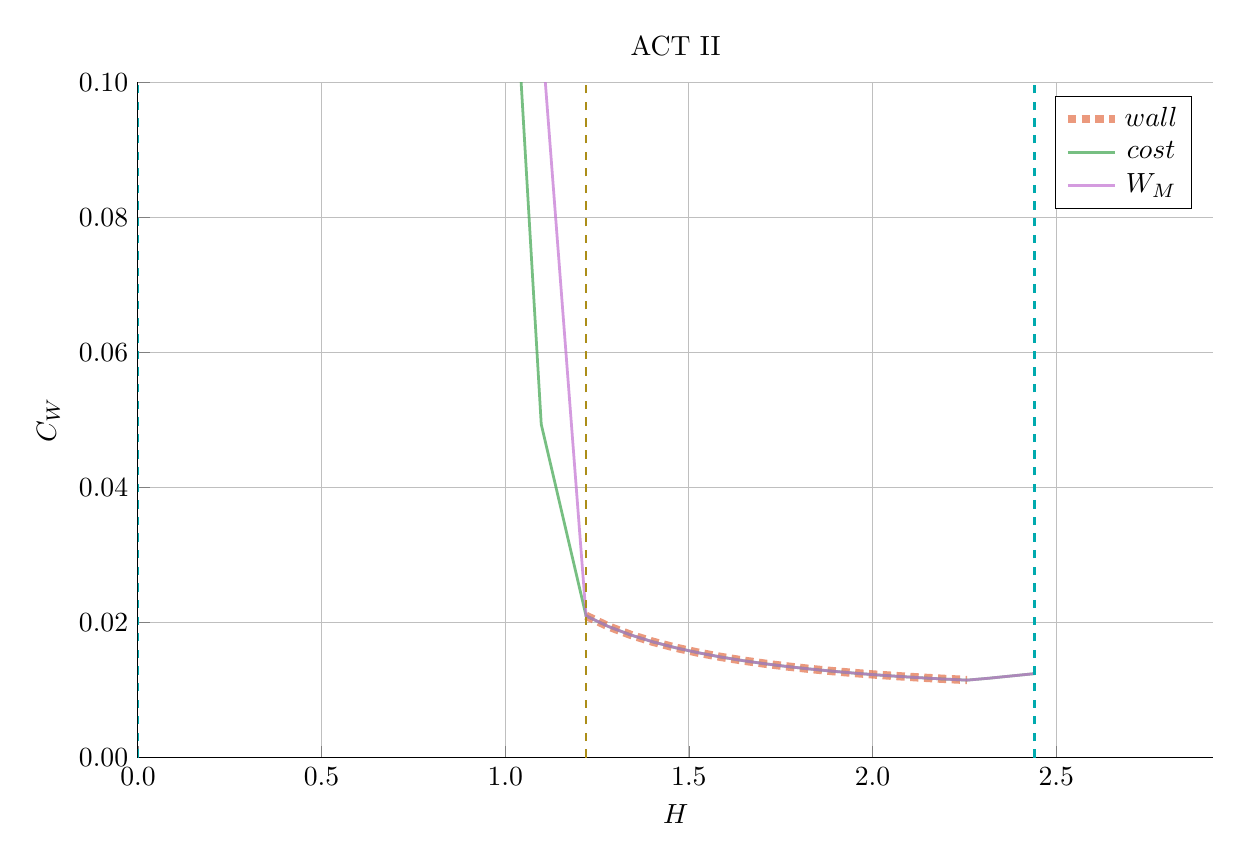
\begin{tikzpicture}[]
\begin{axis}[height = {101.6mm}, ylabel = {${C}_{W}$}, title = {ACT II}, xmin = {0.0}, xmax = {2.928}, ymax = {0.1}, xlabel = {${H}$}, {unbounded coords=jump, scaled x ticks = false, xticklabel style={rotate = 0}, xmajorgrids = true, xtick = {0.0,0.5,1.0,1.5,2.0,2.5}, xticklabels = {0.0,0.5,1.0,1.5,2.0,2.5}, xtick align = inside, axis lines* = left, scaled y ticks = false, yticklabel style={rotate = 0}, ymajorgrids = true, ytick = {0.0,0.02,0.04,0.06,0.08,0.1}, yticklabels = {0.00,0.02,0.04,0.06,0.08,0.10}, ytick align = inside, axis lines* = left,     xshift = 0.0mm,
    yshift = 0.0mm,
    axis background/.style={fill={rgb,1:red,1.00000000;green,1.00000000;blue,1.00000000}}
, colorbar style={title=}}, ymin = {0.0}, width = {152.4mm}]\addplot+ [color = {rgb,1:red,0.88887350;green,0.43564919;blue,0.27812294},
draw opacity=0.7,
line width=3,
dotted,mark = none,
mark size = 2.0,
mark options = {
    color = {rgb,1:red,0.00000000;green,0.00000000;blue,0.00000000}, draw opacity = 0.7,
    fill = {rgb,1:red,0.88887350;green,0.43564919;blue,0.27812294}, fill opacity = 0.7,
    line width = 1,
    rotate = 0,
    solid
}]coordinates {
(1.22, 0.021005512518330174)
(1.281, 0.01942744270360855)
(1.342, 0.018170389811630824)
(1.403, 0.017139710886836464)
(1.464, 0.01627794436788193)
(1.525, 0.015546450836866612)
(1.586, 0.014919600022944367)
(1.647, 0.014377436937475022)
(1.708, 0.013905581766222853)
(1.769, 0.01349265356023887)
(1.83, 0.013129558656358339)
(1.891, 0.01280891244140467)
(1.952, 0.012524569645508304)
(2.013, 0.01227184717788876)
(2.074, 0.012046102834086084)
(2.135, 0.01184360516877147)
(2.196, 0.011661349792575638)
(2.257, 0.011496773538316084)
};
\addlegendentry{$wall$}
\addplot+ [color = {rgb,1:red,0.24222430;green,0.64327509;blue,0.30444865},
draw opacity=0.7,
line width=1,
solid,mark = none,
mark size = 2.0,
mark options = {
    color = {rgb,1:red,0.00000000;green,0.00000000;blue,0.00000000}, draw opacity = 0.7,
    fill = {rgb,1:red,0.24222430;green,0.64327509;blue,0.30444865}, fill opacity = 0.7,
    line width = 1,
    rotate = 0,
    solid
}]coordinates {
(1.037, 0.10576482650233505)
(1.098, 0.04935829436307264)
(1.22, 0.020990970199014802)
(1.281, 0.0194129595370893)
(1.342, 0.01815662533322952)
(1.403, 0.01712672739309554)
(1.464, 0.016265578765863785)
(1.525, 0.015534719386234706)
(1.586, 0.014908297877268767)
(1.647, 0.014366575271189693)
(1.708, 0.013895114510245749)
(1.769, 0.013482541510434981)
(1.83, 0.013119766959557726)
(1.891, 0.012796621459369077)
(1.952, 0.012503284271399288)
(2.013, 0.012246990247871287)
(2.074, 0.012019443303647051)
(2.135, 0.011815835760118812)
(2.196, 0.011632962604193957)
(2.257, 0.011474758216077388)
(2.318, 0.011765579200211946)
(2.379, 0.012101340215422274)
(2.44, 0.012432978177363389)
};
\addlegendentry{$cost$}
\addplot+ [color = {rgb,1:red,0.76444018;green,0.44411178;blue,0.82429754},
draw opacity=0.7,
line width=1,
solid,mark = none,
mark size = 2.0,
mark options = {
    color = {rgb,1:red,0.00000000;green,0.00000000;blue,0.00000000}, draw opacity = 0.7,
    fill = {rgb,1:red,0.76444018;green,0.44411178;blue,0.82429754}, fill opacity = 0.7,
    line width = 1,
    rotate = 0,
    solid
}]coordinates {
(1.098, 0.10789687618345375)
(1.22, 0.020993563020398034)
(1.281, 0.019414381524971283)
(1.342, 0.018157569810455732)
(1.403, 0.017127496371177657)
(1.464, 0.016266077641847662)
(1.525, 0.015535219465132215)
(1.586, 0.014908546212398566)
(1.647, 0.014366740003006752)
(1.708, 0.013895218421357018)
(1.769, 0.01348260263682947)
(1.83, 0.013119799308255348)
(1.891, 0.0127993859843838)
(1.952, 0.012506614611284711)
(2.013, 0.01224686415179682)
(2.074, 0.012019222925033022)
(2.135, 0.011815568425293648)
(2.196, 0.011632678053496345)
(2.257, 0.011474127813480542)
(2.318, 0.011765572318494604)
(2.379, 0.012101333413489)
(2.44, 0.012432971811628111)
};
\addlegendentry{$W_M$}
\addplot+ [color = {rgb,1:red,0.67554396;green,0.55566233;blue,0.09423434},
draw opacity=1.0,
line width=1,
dashed,mark = none,
mark size = 2.0,
mark options = {
    color = {rgb,1:red,0.00000000;green,0.00000000;blue,0.00000000}, draw opacity = 1.0,
    fill = {rgb,1:red,0.67554396;green,0.55566233;blue,0.09423434}, fill opacity = 1.0,
    line width = 1,
    rotate = 0,
    solid
},forget plot]coordinates {
(1.22, 0.0)
(1.22, 0.1)
};
\addplot+ [color = {rgb,1:red,0.00000048;green,0.66575898;blue,0.68099695},
draw opacity=1.0,
line width=1,
dashed,mark = none,
mark size = 2.0,
mark options = {
    color = {rgb,1:red,0.00000000;green,0.00000000;blue,0.00000000}, draw opacity = 1.0,
    fill = {rgb,1:red,0.00000048;green,0.66575898;blue,0.68099695}, fill opacity = 1.0,
    line width = 1,
    rotate = 0,
    solid
},forget plot]coordinates {
(0.0, 0.0)
(0.0, 0.1)
};
\addplot+ [color = {rgb,1:red,0.00000048;green,0.66575898;blue,0.68099695},
draw opacity=1.0,
line width=1,
dashed,mark = none,
mark size = 2.0,
mark options = {
    color = {rgb,1:red,0.00000000;green,0.00000000;blue,0.00000000}, draw opacity = 1.0,
    fill = {rgb,1:red,0.00000048;green,0.66575898;blue,0.68099695}, fill opacity = 1.0,
    line width = 1,
    rotate = 0,
    solid
},forget plot]coordinates {
(2.44, 0.0)
(2.44, 0.1)
};
\end{axis}

\end{tikzpicture}

    \end{adjustbox}
        \caption{ACT II H Sweep}
    \end{subfigure}
    \hfill \hfill ~\\ ~\\ ~\\
    \begin{subfigure}[t]{0.425\textwidth}
        \centering
		\begin{adjustbox}{width=\textwidth}
			\Large
			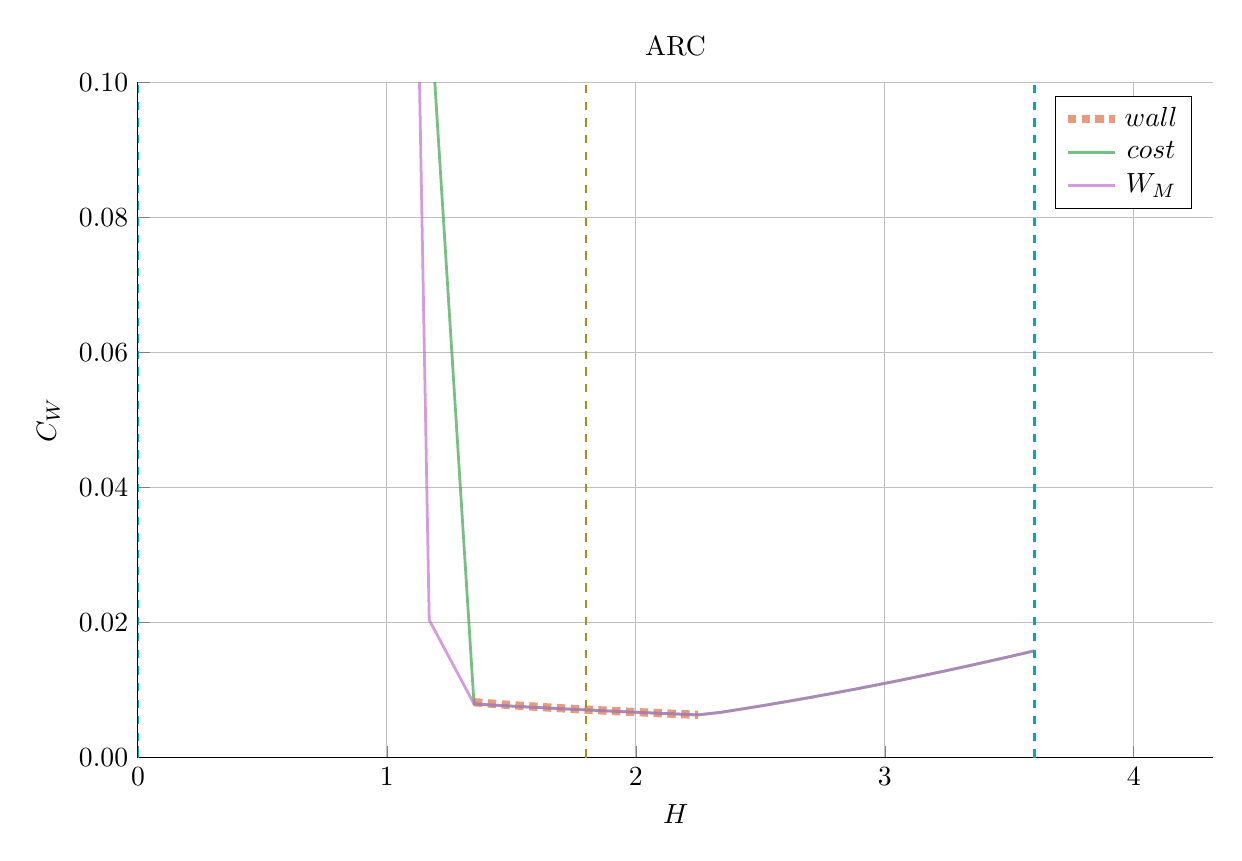
\begin{tikzpicture}[]
\begin{axis}[height = {101.6mm}, ylabel = {${C}_{W}$}, title = {ARC}, xmin = {0.0}, xmax = {4.32}, ymax = {0.1}, xlabel = {${H}$}, {unbounded coords=jump, scaled x ticks = false, xticklabel style={rotate = 0}, xmajorgrids = true, xtick = {0.0,1.0,2.0,3.0,4.0}, xticklabels = {0,1,2,3,4}, xtick align = inside, axis lines* = left, scaled y ticks = false, yticklabel style={rotate = 0}, ymajorgrids = true, ytick = {0.0,0.02,0.04,0.06,0.08,0.1}, yticklabels = {0.00,0.02,0.04,0.06,0.08,0.10}, ytick align = inside, axis lines* = left,     xshift = 0.0mm,
    yshift = 0.0mm,
    axis background/.style={fill={rgb,1:red,1.00000000;green,1.00000000;blue,1.00000000}}
, colorbar style={title=}}, ymin = {0.0}, width = {152.4mm}]\addplot+ [color = {rgb,1:red,0.88887350;green,0.43564919;blue,0.27812294},
draw opacity=0.7,
line width=3,
dotted,mark = none,
mark size = 2.0,
mark options = {
    color = {rgb,1:red,0.00000000;green,0.00000000;blue,0.00000000}, draw opacity = 0.7,
    fill = {rgb,1:red,0.88887350;green,0.43564919;blue,0.27812294}, fill opacity = 0.7,
    line width = 1,
    rotate = 0,
    solid
}]coordinates {
(1.35, 0.008207241762396246)
(1.44, 0.00793667759257354)
(1.53, 0.0076997912429461225)
(1.62, 0.007486816554981894)
(1.71, 0.007291648689881567)
(1.8, 0.007110333347796811)
(1.89, 0.006940248814588952)
(1.98, 0.006779633349026309)
(2.07, 0.006627297197584387)
(2.16, 0.006482438866566955)
(2.25, 0.006344768968841929)
};
\addlegendentry{$wall$}
\addplot+ [color = {rgb,1:red,0.24222430;green,0.64327509;blue,0.30444865},
draw opacity=0.7,
line width=1,
solid,mark = none,
mark size = 2.0,
mark options = {
    color = {rgb,1:red,0.00000000;green,0.00000000;blue,0.00000000}, draw opacity = 0.7,
    fill = {rgb,1:red,0.24222430;green,0.64327509;blue,0.30444865}, fill opacity = 0.7,
    line width = 1,
    rotate = 0,
    solid
}]coordinates {
(1.08, 0.1656933786109522)
(1.35, 0.007956028922350611)
(1.44, 0.007759662745290108)
(1.53, 0.007574913322065527)
(1.62, 0.00739885086770846)
(1.71, 0.0072297906534508185)
(1.8, 0.007066784363464752)
(1.89, 0.00690932755478892)
(1.98, 0.006757201835765392)
(2.07, 0.006610359300650354)
(2.16, 0.0064688545800951625)
(2.25, 0.006332913629979953)
(2.34, 0.00670268792962123)
(2.43, 0.0072243580642261445)
(2.52, 0.007766406785339575)
(2.61, 0.008328785580854575)
(2.7, 0.008911412315791628)
(2.79, 0.00951417119398493)
(2.88, 0.010136912409268534)
(2.97, 0.010779452862615483)
(3.06, 0.011441576670944502)
(3.15, 0.012123036438828786)
(3.24, 0.012823554577929932)
(3.33, 0.0135428254017145)
(3.42, 0.014280516598644705)
(3.51, 0.015036271676563144)
(3.6, 0.01580971210009804)
};
\addlegendentry{$cost$}
\addplot+ [color = {rgb,1:red,0.76444018;green,0.44411178;blue,0.82429754},
draw opacity=0.7,
line width=1,
solid,mark = none,
mark size = 2.0,
mark options = {
    color = {rgb,1:red,0.00000000;green,0.00000000;blue,0.00000000}, draw opacity = 0.7,
    fill = {rgb,1:red,0.76444018;green,0.44411178;blue,0.82429754}, fill opacity = 0.7,
    line width = 1,
    rotate = 0,
    solid
}]coordinates {
(1.08, 0.20419403931121408)
(1.17, 0.02038194154635263)
(1.35, 0.007952462446561684)
(1.44, 0.007756882763096937)
(1.53, 0.007572765485693452)
(1.62, 0.007397214242173672)
(1.71, 0.007228584574974498)
(1.8, 0.007065962995902896)
(1.89, 0.006908746287963411)
(1.98, 0.006756833824238413)
(2.07, 0.0066101524637499)
(2.16, 0.006468686518064958)
(2.25, 0.006332754951862069)
(2.34, 0.00670262687626648)
(2.43, 0.007224172350640052)
(2.52, 0.007766066748915404)
(2.61, 0.008328266004035769)
(2.7, 0.008910694013555907)
(2.79, 0.009513241975770496)
(2.88, 0.010135768084513136)
(2.97, 0.010778097603257038)
(3.06, 0.011440023505553681)
(3.15, 0.01212130721887041)
(3.24, 0.012821680052634414)
(3.33, 0.013540844476435391)
(3.42, 0.014278476232750113)
(3.51, 0.015034225935616565)
(3.6, 0.01580772161808181)
};
\addlegendentry{$W_M$}
\addplot+ [color = {rgb,1:red,0.67554396;green,0.55566233;blue,0.09423434},
draw opacity=1.0,
line width=1,
dashed,mark = none,
mark size = 2.0,
mark options = {
    color = {rgb,1:red,0.00000000;green,0.00000000;blue,0.00000000}, draw opacity = 1.0,
    fill = {rgb,1:red,0.67554396;green,0.55566233;blue,0.09423434}, fill opacity = 1.0,
    line width = 1,
    rotate = 0,
    solid
},forget plot]coordinates {
(1.8, 0.0)
(1.8, 0.1)
};
\addplot+ [color = {rgb,1:red,0.00000048;green,0.66575898;blue,0.68099695},
draw opacity=1.0,
line width=1,
dashed,mark = none,
mark size = 2.0,
mark options = {
    color = {rgb,1:red,0.00000000;green,0.00000000;blue,0.00000000}, draw opacity = 1.0,
    fill = {rgb,1:red,0.00000048;green,0.66575898;blue,0.68099695}, fill opacity = 1.0,
    line width = 1,
    rotate = 0,
    solid
},forget plot]coordinates {
(0.0, 0.0)
(0.0, 0.1)
};
\addplot+ [color = {rgb,1:red,0.00000048;green,0.66575898;blue,0.68099695},
draw opacity=1.0,
line width=1,
dashed,mark = none,
mark size = 2.0,
mark options = {
    color = {rgb,1:red,0.00000000;green,0.00000000;blue,0.00000000}, draw opacity = 1.0,
    fill = {rgb,1:red,0.00000048;green,0.66575898;blue,0.68099695}, fill opacity = 1.0,
    line width = 1,
    rotate = 0,
    solid
},forget plot]coordinates {
(3.6, 0.0)
(3.6, 0.1)
};
\end{axis}

\end{tikzpicture}

		\end{adjustbox}
        \caption{ARC H Sweep}
    \end{subfigure} ~\\ ~\\ ~\\
    \caption{ARC and ACT Studies Cost Dependence on the H Factor} ~\\
    \small The cost of steady-state reactors can usually be reduced by increasing the enhancement factor. As shown, though, none of these reactors are possible at the standard H = 1 value!
	\label{fig:act_h_cost}
\end{figure*}

\subsubsection{ACT I -- Advanced Physics and Engineering}

ACT 1 is the ARIES study that assumes advanced physics and engineering design parameters. Although this paper's model does a \replaced{fair job recovering}{good job matching} the results from their paper -- see \cref{table:act_1,fig:act_1_comparison} -- it does show what optimistic design really means. As can be seen, this design actually only surpasses the minimum possible toroidal field strength by as less than a Tesla! Practically, this means \replaced{their}{the} reactor is barely realizable. \added{Trying to build a 5T device would not be possible using their stated reactor input parameters.}

\subsubsection{ACT II -- Conservative Physics and Engineering}

ARIES more conservative design -- ACT II -- is much more like ARC in nature. From \cref{fig:act_2_comparison}, it is obvious the paper's model is basically right on top of the reactor curve made using Fussy.jl.  Much like ARC, too, it shows how the model overestimates fusion power and underestimates bootstrap fraction due to their selection of a pedestal profile for plasma temperature. This can be seen in \cref{table:act_2}.

\subsection{Benchmarking with the Process DEMO Designs}

The PROCESS team's prospective designs for successors to ITER constitute the final set of model comparisons: the steady-state and pulsed DEMO reactors. As this paper is designed to compare these modes of operation, this study proves most \replaced{informative.}{fruitful.} It also highlights how common model decisions can dramatically alter what reactors come out of the solvers.

The first discrepancy is how the PROCESS team defines the loss term in the ELMy H-Mode scaling law. As shown in their paper, they actually subtract out a Bremsstrahlung component, while leaving the fitting coefficients the same. \cite{process} After modifying Fussy.jl to incorporate this definition, the steady-state reactor is easily reproducible in $R_0$ -- $B_0$ slice of reactor space.
\begin{equation}
	\label{eq:pl_demo}
	P_L^{DEMO} = P_{src} - P_{BR}
\end{equation}

Unlike the steady-state case, however, the modified power loss term does not fix the pulsed case, as it actually draws the reactor curves further from the design in their paper. As such, it is flux balance that is now the main culprit for discrepancies between the two models. This makes sense, as this model uses highly simplified source terms -- namely neglecting anything but the central solenoid and PF coils (as well as ignoring crucial physics for these two components). Even acknowledging the differences between the two models, Fussy.jl still does \replaced{reasonably}{remarkably} well at reproducing their much more sophisticated coding framework.

The final point to make is about selecting optimum points to build as the \replaced{dynamic}{floating} variables are allowed to make curves through reactor space. Up to this point, only steady-state tokamak designs have been explored. In every single one of these, though, the paper values have been very close to the point where the beta curves and wall loading curves cross. This is because they all result in the minimum cost-per-watt.

For pulsed designs, on the other hand, kink curves start to appear for low magnetic field strengths. Just as beta-wall intersections were optimum places to design for low cost-per-watt ($C_W$) reactors, these beta-kink intersections will prove to be the place where minimum capital cost ($W_M$) reactors usually occur. \added{This is discussed in more detail in \cref{subsection:design_point}.}

\subsubsection{DEMO Steady -- A Steady-State ITER Successor}

\deleted{Hands down, this DEMO Steady reactor is the worst modeled reactor using Fussy.jl. As mentioned previously, though, some of the discrepancy was removed by using the PROCESS team's modified version of heat loss. This heavily corrected the $R_0$ -- $B_0$ curve, but had no effect on the $I_P$ -- $\overline T$ one. An interesting aside is that these curves actually show how steady current is independent of \replaced{limiting}{secondary} constraint (as noted).}

\added{As shown in \cref{fig:demo_steady_comparison,table:demo_steady}, the DEMO steady reactor is the design captured worst by the Fussy.jl model. Some discrepancy, however can be removed by using the PROCESS team's modified version of heat loss, as given by \cref{eq:pl_demo}.\cite{process} Although not supported by the official ITER database fit,\cite{iter_confinement} the PROCESS team reduces the absorbed power by the Bremsstrahlung power\cite{process_rad} -- which can lengthen $\tau_E$ by more than 25\%.\cite{inputfile} }

\added{With this correction, the $R_0$ -- $B_0$ curve is drawn to be right on top of their model's design. The same cannot be said for the $I_P$ -- $\overline T$ curve as steady current was shown to have little dependence on tokamak configuration ($R_0$ and $B_0$) and, correspondingly, the limiting constraint (e.g. \texttt{beta} and \texttt{wall}). }

\added{Note that the labels of \texttt{modified} and \texttt{pulsed} are slightly obscure in this context. Pulsed, for starters, is actually the generalized solver that does not rely on self-consistent current drive (i.e. in $\eta_{CD}$). The modified label is then when the pulsed solver uses the $P_L^{DEMO}$ value in approximating heat conductive losses.}

\subsubsection{DEMO Pulsed -- A Pulsed ITER Successor}

This pulsed version of DEMO is the only reactor in our collection that is not run in steady-state. As such, it may be the most important one \added{(i.e. it is the only pulsed reactor)}. The first \replaced{observation from \cref{fig:demo_pulsed_comparison}}{thing that is abundantly clear} is that this design actually has no valid wall loading portion -- only a kink and beta curve exist! Even so, the results match pretty well (see \cref{table:demo_pulsed}). It should be noted, though, that this current drive is treated as an input and not solved self-consistently.

\clearpage

\newpage

\begin{figure*}[t!]
    \centering
    \hfill
    \begin{subfigure}[t]{0.45\textwidth}
        \centering
    \begin{adjustbox}{width=\textwidth}
      \Large
      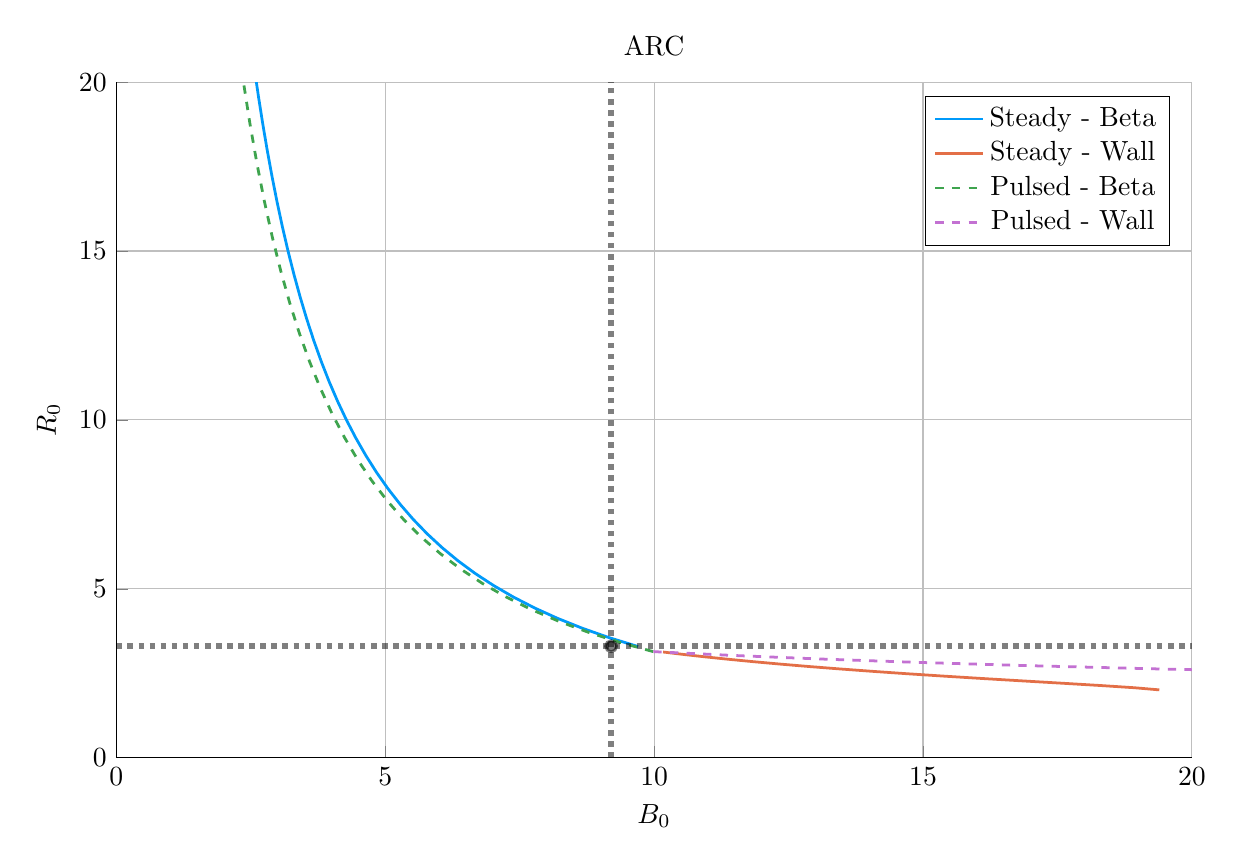
\begin{tikzpicture}[]
\begin{axis}[height = {101.6mm}, ylabel = {${R}_{0}$}, title = {ARC}, xmin = {0.0}, xmax = {20.0}, ymax = {20.0}, xlabel = {${B}_{0}$}, {unbounded coords=jump, scaled x ticks = false, xticklabel style={rotate = 0}, xmajorgrids = true, xtick = {0.0,5.0,10.0,15.0,20.0}, xticklabels = {0,5,10,15,20}, xtick align = inside, axis lines* = left, scaled y ticks = false, yticklabel style={rotate = 0}, ymajorgrids = true, ytick = {0.0,5.0,10.0,15.0,20.0}, yticklabels = {0,5,10,15,20}, ytick align = inside, axis lines* = left,     xshift = 0.0mm,
    yshift = 0.0mm,
    axis background/.style={fill={rgb,1:red,1.00000000;green,1.00000000;blue,1.00000000}}
, colorbar style={title=}}, ymin = {0.0}, width = {152.4mm}]\addplot+ [color = {rgb,1:red,0.00000000;green,0.60560316;blue,0.97868012},
draw opacity=1.0,
line width=1,
solid,mark = none,
mark size = 2.0,
mark options = {
    color = {rgb,1:red,0.00000000;green,0.00000000;blue,0.00000000}, draw opacity = 1.0,
    fill = {rgb,1:red,0.00000000;green,0.60560316;blue,0.97868012}, fill opacity = 1.0,
    line width = 1,
    rotate = 0,
    solid
}]coordinates {
(9.701206080853105, 3.2904233285656006)
(9.162315904693079, 3.553631706046861)
(8.664301107137337, 3.8315748016260343)
(8.203576462497304, 4.124583886864978)
(7.776718537485166, 4.433072975674755)
(7.380720231870917, 4.75741949036414)
(7.012886014999712, 5.097987291342331)
(6.670795005901889, 5.4551257000070565)
(6.352268997292712, 5.829168567645448)
(6.055344682097163, 6.220433393277178)
(5.778249464564785, 6.629220493040615)
(5.519380338856715, 7.05581222339423)
(5.2772854007125325, 7.500472260074458)
(5.050647625972996, 7.963444934423652)
(4.838270606140816, 8.444954628380609)
(4.639065978019038, 8.94520522910952)
(4.4520423235376105, 9.464379643936518)
(4.276295348572609, 10.002639375969222)
(4.110999177018484, 10.56012416048812)
(3.9553986195015125, 11.136951661929974)
(3.8088022956698633, 11.733217231026282)
(3.6705765055641186, 12.34899372141899)
(3.54013975965751, 12.984331364849716)
(3.4169578891619192, 13.639257703809928)
(3.30053966845824, 14.313777580345645)
(3.1904328903033052, 15.007873179535935)
(3.086220842019516, 15.721504126002731)
(2.9875191373772063, 16.45460763166718)
(2.8939728644914635, 17.207098692842226)
(2.8052540149097247, 17.97887033463821)
(2.7210591632720242, 18.7697939005645)
(2.6411073705789065, 19.579719385129263)
(2.565138287279709, 20.40847580717446)
(2.492910435164382, 21.255871621630877)
(2.4241996494611984, 22.12169516733927)
(2.3587976646588236, 23.0057151485579)
(2.296510829425685, 23.907681147764652)
(2.237158937627476, 24.827324167354146)
(2.180574163874242, 25.764357197843207)
(2.126600093288366, 26.71847581021091)
(2.075090836295778, 27.689358770027713)
(2.0259102202234582, 28.676668671060817)
(1.978931050353818, 29.68005258608471)
(1.9340344338545452, 30.69914273267572)
(1.8911091606836798, 31.733557151818793)
(1.8500511361739687, 32.78290039722107)
(1.8107628605384507, 33.846764233283025)
(1.773152951016952, 34.92472833975579)
(1.7371357028100902, 36.01636102117257)
(1.7026306853269466, 37.121219919229354)
(1.6695623706125668, 38.23885272635799)
(1.6378597911249178, 39.368797898817405)
(1.607456224302725, 40.51058536770822)
(1.5782889016090462, 41.663737246396295)
(1.5502987399539199, 42.82776853291479)
(1.5234300935954943, 44.00218780599217)
(1.4976305247952577, 45.18649791343829)
(1.4728505916614916, 46.38019665170201)
(1.4490436517578602, 47.58277743549339)
(1.4261656801829077, 48.79372995643627)
};
\addlegendentry{Steady - Beta}
\addplot+ [color = {rgb,1:red,0.88887350;green,0.43564919;blue,0.27812294},
draw opacity=1.0,
line width=1,
solid,mark = none,
mark size = 2.0,
mark options = {
    color = {rgb,1:red,0.00000000;green,0.00000000;blue,0.00000000}, draw opacity = 1.0,
    fill = {rgb,1:red,0.88887350;green,0.43564919;blue,0.27812294}, fill opacity = 1.0,
    line width = 1,
    rotate = 0,
    solid
}]coordinates {
(19.394007482712425, 2.006855814841082)
(18.932196567189358, 2.070220226465634)
(18.296989378345195, 2.1362327099649083)
(17.587029315408756, 2.2039322514902886)
(16.847882407994106, 2.272885741349308)
(16.111374502564406, 2.3427307443133163)
(15.396027314547156, 2.4132115621474344)
(14.710952688793137, 2.484165095168367)
(14.06168447794857, 2.555449485048069)
(13.450465418483889, 2.6269568263788754)
(12.877644538645335, 2.6986005527245354)
(12.342394470642008, 2.7703103261458715)
(11.843182246608265, 2.8420284550528074)
(11.376441269625893, 2.9137564749008216)
(10.944966372727551, 2.985307257194073)
(10.541663878705513, 3.056795384934831)
(10.165908182236457, 3.128148092221394)
};
\addlegendentry{Steady - Wall}
\addplot+ [color = {rgb,1:red,0.24222430;green,0.64327509;blue,0.30444865},
draw opacity=1.0,
line width=1,
dashed,mark = none,
mark size = 2.0,
mark options = {
    color = {rgb,1:red,0.00000000;green,0.00000000;blue,0.00000000}, draw opacity = 1.0,
    fill = {rgb,1:red,0.24222430;green,0.64327509;blue,0.30444865}, fill opacity = 1.0,
    line width = 1,
    rotate = 0,
    solid
}]coordinates {
(9.980483622051658, 3.1402982942956537)
(9.392786903460065, 3.3984668375583613)
(8.79273598103983, 3.7029994270206985)
(8.23820290909994, 4.029752381934837)
(7.725182218401588, 4.380005330007902)
(7.250078106370205, 4.755088191072525)
(6.80965553466646, 5.15638156809462)
(6.400998063035608, 5.585317075247801)
(6.0214713600430425, 6.043377623224966)
(5.668691517461799, 6.532097691007738)
(5.340497445229901, 7.053063624618788)
(5.034926745580058, 7.607914017422467)
(4.750194564008521, 8.198340243900201)
(4.484674995755211, 8.826087240213646)
(4.236884692979903, 9.49295465115087)
(4.00546837264544, 10.200798495308337)
(3.7891859704718387, 10.951533539957822)
(3.5869012239550364, 11.747136625739826)
(3.3975714987448393, 12.589651241396528)
(3.2202386987489797, 13.481193723261853)
(3.0540211220494466, 14.423961547290066)
(2.8981061427709687, 15.420244298711943)
(2.7517436139566023, 16.472438053930638)
(2.6142398986781377, 17.58306410230943)
(2.4849524463010138, 18.754793188384546)
(2.363284838174807, 19.990476791576892)
(2.248682232019848, 21.293187416028662)
(2.140627136740878, 22.666270490916787)
(2.038635448877246, 24.113411362836906)
(1.9422526775794744, 25.638722123308433)
(1.8510502754751532, 27.246854857488287)
(1.7646219756564088, 28.94315065234289)
(1.6825800061969869, 30.73383791051506)
(1.6045510059627948, 32.62630011975996)
(1.53017138625397, 34.629443897654504)
(1.4590817483192686, 36.754215952550474)
(1.3909197311384796, 39.01434852880224)
(1.3253102336217724, 41.42746903285954)
(1.261851128383913, 44.01681696754988)
(1.20009089049112, 46.81403058684408)
(1.1394908096975784, 49.863950342519615)
};
\addlegendentry{Pulsed - Beta}
\addplot+ [color = {rgb,1:red,0.76444018;green,0.44411178;blue,0.82429754},
draw opacity=1.0,
line width=1,
dashed,mark = none,
mark size = 2.0,
mark options = {
    color = {rgb,1:red,0.00000000;green,0.00000000;blue,0.00000000}, draw opacity = 1.0,
    fill = {rgb,1:red,0.76444018;green,0.44411178;blue,0.82429754}, fill opacity = 1.0,
    line width = 1,
    rotate = 0,
    solid
}]coordinates {
(29.27715761652869, 2.3448804182939873)
(25.4410619834368, 2.4377937236066716)
(22.158819835998365, 2.5322208586485804)
(19.342453256965573, 2.628163744265164)
(16.919364280634177, 2.7256238396687067)
(14.829378672669455, 2.8246020951898183)
(13.022412368922526, 2.9250989082568273)
(11.456617692058645, 3.0271140820266207)
(10.096901921254785, 3.1306467862637533)
(9.980483622051658, 3.1402982942956537)
};
\addlegendentry{Pulsed - Wall}
\addplot+ [color = {rgb,1:red,0.00000000;green,0.00000000;blue,0.00000000},
draw opacity=0.5,
line width=2,
dotted,mark = none,
mark size = 2.0,
mark options = {
    color = {rgb,1:red,0.00000000;green,0.00000000;blue,0.00000000}, draw opacity = 0.5,
    fill = {rgb,1:red,0.00000000;green,0.00000000;blue,0.00000000}, fill opacity = 0.5,
    line width = 1,
    rotate = 0,
    solid
},forget plot]coordinates {
(0.0, 3.3)
(20.0, 3.3)
};
\addplot+ [color = {rgb,1:red,0.00000000;green,0.00000000;blue,0.00000000},
draw opacity=0.5,
line width=2,
dotted,mark = none,
mark size = 2.0,
mark options = {
    color = {rgb,1:red,0.00000000;green,0.00000000;blue,0.00000000}, draw opacity = 0.5,
    fill = {rgb,1:red,0.00000000;green,0.00000000;blue,0.00000000}, fill opacity = 0.5,
    line width = 1,
    rotate = 0,
    solid
},forget plot]coordinates {
(9.2, 0.0)
(9.2, 20.0)
};
\addplot+[draw=none, color = {rgb,1:red,0.00000000;green,0.00000000;blue,0.00000000},
draw opacity=0.5,
line width=0,
solid,mark = *,
mark size = 2.0,
mark options = {
    color = {rgb,1:red,0.00000000;green,0.00000000;blue,0.00000000}, draw opacity = 0.5,
    fill = {rgb,1:red,0.00000000;green,0.00000000;blue,0.00000000}, fill opacity = 0.5,
    line width = 1,
    rotate = 0,
    solid
},forget plot] coordinates {
(9.2, 3.3)
};
\end{axis}

\end{tikzpicture}

    \end{adjustbox}
        \caption{$R_0$ vs $B_0$}
    \end{subfigure}
    \hfill
    \begin{subfigure}[t]{0.45\textwidth}
        \centering
    \begin{adjustbox}{width=\textwidth}
      \Large
      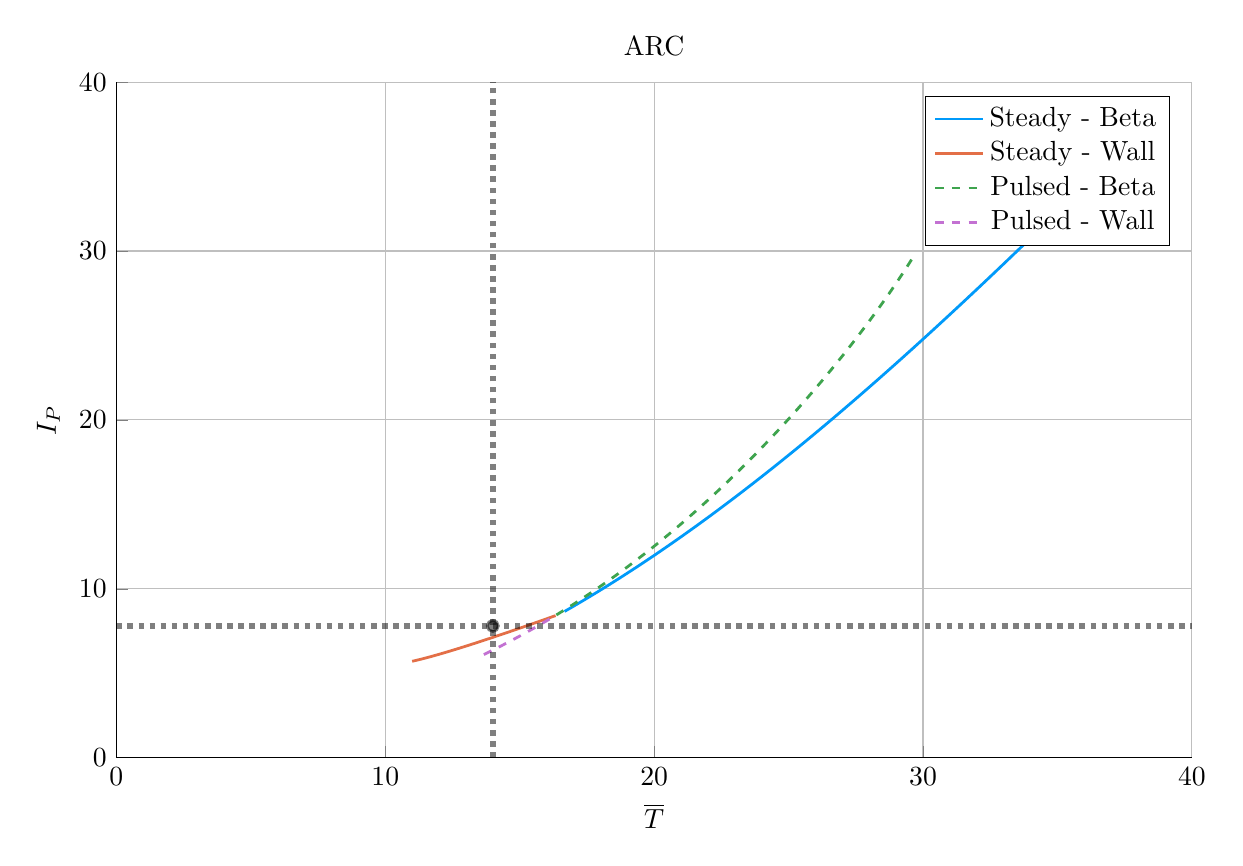
\begin{tikzpicture}[]
\begin{axis}[height = {101.6mm}, ylabel = {${I}_{P}$}, title = {ARC}, xmin = {0.0}, xmax = {40.0}, ymax = {40.0}, xlabel = {$\overline {T}$}, {unbounded coords=jump, scaled x ticks = false, xticklabel style={rotate = 0}, xmajorgrids = true, xtick = {0.0,10.0,20.0,30.0,40.0}, xticklabels = {0,10,20,30,40}, xtick align = inside, axis lines* = left, scaled y ticks = false, yticklabel style={rotate = 0}, ymajorgrids = true, ytick = {0.0,10.0,20.0,30.0,40.0}, yticklabels = {0,10,20,30,40}, ytick align = inside, axis lines* = left,     xshift = 0.0mm,
    yshift = 0.0mm,
    axis background/.style={fill={rgb,1:red,1.00000000;green,1.00000000;blue,1.00000000}}
, colorbar style={title=}}, ymin = {0.0}, width = {152.4mm}]\addplot+ [color = {rgb,1:red,0.00000000;green,0.60560316;blue,0.97868012},
draw opacity=1.0,
line width=1,
solid,mark = none,
mark size = 2.0,
mark options = {
    color = {rgb,1:red,0.00000000;green,0.00000000;blue,0.00000000}, draw opacity = 1.0,
    fill = {rgb,1:red,0.00000000;green,0.60560316;blue,0.97868012}, fill opacity = 1.0,
    line width = 1,
    rotate = 0,
    solid
}]coordinates {
(16.666666666666668, 8.658343870907427)
(17.0, 8.964855141636448)
(17.333333333333332, 9.277118721367206)
(17.666666666666668, 9.595036914426)
(18.0, 9.918585776352757)
(18.333333333333332, 10.247718935951552)
(18.666666666666668, 10.582387319200262)
(19.0, 10.922539274323045)
(19.333333333333332, 11.26812069483817)
(19.666666666666668, 11.61907514056121)
(20.0, 11.975343956529299)
(20.333333333333332, 12.336866389803589)
(20.666666666666668, 12.703579704100664)
(21.0, 13.07541929220057)
(21.333333333333332, 13.452318786079019)
(21.666666666666668, 13.834210164711733)
(22.0, 14.221023859501257)
(22.333333333333332, 14.61268885728139)
(22.666666666666668, 15.009132800857182)
(23.0, 15.410282087044596)
(23.333333333333332, 15.816061962178953)
(23.666666666666668, 16.226396615066992)
(24.0, 16.64120926736311)
(24.333333333333332, 17.060422261356294)
(24.666666666666668, 17.483957145159597)
(25.0, 17.91173475530017)
(25.333333333333332, 18.343675296712746)
(25.666666666666668, 18.77969842014449)
(26.0, 19.2197232969848)
(26.333333333333332, 19.663668691537165)
(26.666666666666668, 20.11145303075519)
(27.0, 20.562994471468567)
(27.333333333333332, 21.018210965128485)
(27.666666666666668, 21.477020320105293)
(28.0, 21.939340261574117)
(28.333333333333332, 22.405088489026962)
(28.666666666666668, 22.874182731452617)
(29.0, 23.34654080022686)
(29.333333333333332, 23.82208063975841)
(29.666666666666668, 24.300720375936947)
(30.0, 24.782378362431352)
(30.333333333333332, 25.26697322488704)
(30.666666666666668, 25.754423903072542)
(31.0, 26.244649691026318)
(31.333333333333332, 26.737570275254438)
(31.666666666666668, 27.233105771031717)
(32.0, 27.731176756857092)
(32.333333333333336, 28.23170430711659)
(32.666666666666664, 28.734610023004112)
(33.0, 29.23981606175298)
(33.333333333333336, 29.747245164229085)
(33.666666666666664, 30.256820680936514)
(34.0, 30.768466596486252)
(34.333333333333336, 31.282107552577845)
(34.666666666666664, 31.797668869543177)
(35.0, 32.31507656650066)
(35.333333333333336, 32.83425738016771)
(35.666666666666664, 33.35513878237846)
(36.0, 33.87764899635294)
(36.333333333333336, 34.40171701176134)
};
\addlegendentry{Steady - Beta}
\addplot+ [color = {rgb,1:red,0.88887350;green,0.43564919;blue,0.27812294},
draw opacity=1.0,
line width=1,
solid,mark = none,
mark size = 2.0,
mark options = {
    color = {rgb,1:red,0.00000000;green,0.00000000;blue,0.00000000}, draw opacity = 1.0,
    fill = {rgb,1:red,0.88887350;green,0.43564919;blue,0.27812294}, fill opacity = 1.0,
    line width = 1,
    rotate = 0,
    solid
}]coordinates {
(11.0, 5.705363947896813)
(11.333333333333334, 5.831631927327359)
(11.666666666666666, 5.971358416795512)
(12.0, 6.120248050030096)
(12.333333333333334, 6.27635241161913)
(12.666666666666666, 6.438084943966173)
(13.0, 6.6043437111573775)
(13.333333333333334, 6.774432932493379)
(13.666666666666666, 6.9477586358526295)
(14.0, 7.123875039246037)
(14.333333333333334, 7.302428845502918)
(14.666666666666666, 7.483135839919747)
(15.0, 7.66576464137543)
(15.333333333333334, 7.850323804140159)
(15.666666666666666, 8.036059275223955)
(16.0, 8.223435700494395)
(16.333333333333332, 8.412159667095638)
};
\addlegendentry{Steady - Wall}
\addplot+ [color = {rgb,1:red,0.24222430;green,0.64327509;blue,0.30444865},
draw opacity=1.0,
line width=1,
dashed,mark = none,
mark size = 2.0,
mark options = {
    color = {rgb,1:red,0.00000000;green,0.00000000;blue,0.00000000}, draw opacity = 1.0,
    fill = {rgb,1:red,0.24222430;green,0.64327509;blue,0.30444865}, fill opacity = 1.0,
    line width = 1,
    rotate = 0,
    solid
}]coordinates {
(16.364160609330686, 8.45211123232532)
(16.666666666666668, 8.749174237506722)
(17.0, 9.084875445329175)
(17.333333333333332, 9.429466194729264)
(17.666666666666668, 9.783065958753857)
(18.0, 10.145791398086809)
(18.333333333333332, 10.517756265001724)
(18.666666666666668, 10.899071333792335)
(19.0, 11.28984436597908)
(19.333333333333332, 11.690180120182706)
(19.666666666666668, 12.100180418434789)
(20.0, 12.519944282916168)
(20.333333333333332, 12.949568159742276)
(20.666666666666668, 13.389146249526421)
(21.0, 13.838770968145022)
(21.333333333333332, 14.298533565526986)
(21.666666666666668, 14.768524935556082)
(22.0, 15.2488366565296)
(22.333333333333332, 15.739562309352701)
(22.666666666666668, 16.240799130174846)
(23.0, 16.752650066058415)
(23.333333333333332, 17.27522631730515)
(23.666666666666668, 17.808650469386293)
(24.0, 18.353060342640163)
(24.333333333333332, 18.908613721362002)
(24.666666666666668, 19.475494169025602)
(25.0, 20.053918198206937)
(25.333333333333332, 20.644144149900036)
(25.666666666666668, 21.246483258877372)
(26.0, 21.861313557471373)
(26.333333333333332, 22.48909752802998)
(26.666666666666668, 23.130404800381292)
(27.0, 23.785941781633092)
(27.333333333333332, 24.456591033172632)
(27.666666666666668, 25.143464707502787)
(28.0, 25.84797885666414)
(28.333333333333332, 26.571959755666764)
(28.666666666666668, 27.3178012356156)
(29.0, 28.088707029156687)
(29.333333333333332, 28.889082725820668)
(29.666666666666668, 29.725209471035893)
};
\addlegendentry{Pulsed - Beta}
\addplot+ [color = {rgb,1:red,0.76444018;green,0.44411178;blue,0.82429754},
draw opacity=1.0,
line width=1,
dashed,mark = none,
mark size = 2.0,
mark options = {
    color = {rgb,1:red,0.00000000;green,0.00000000;blue,0.00000000}, draw opacity = 1.0,
    fill = {rgb,1:red,0.76444018;green,0.44411178;blue,0.82429754}, fill opacity = 1.0,
    line width = 1,
    rotate = 0,
    solid
}]coordinates {
(13.666666666666666, 6.106956435644008)
(14.0, 6.368429153074452)
(14.333333333333334, 6.637611037727747)
(14.666666666666666, 6.914640849606676)
(15.0, 7.199655680909235)
(15.333333333333334, 7.492790823032018)
(15.666666666666666, 7.794179619860046)
(16.0, 8.103953307930404)
(16.333333333333332, 8.422240844292133)
(16.364160609330686, 8.45211123232532)
};
\addlegendentry{Pulsed - Wall}
\addplot+ [color = {rgb,1:red,0.00000000;green,0.00000000;blue,0.00000000},
draw opacity=0.5,
line width=2,
dotted,mark = none,
mark size = 2.0,
mark options = {
    color = {rgb,1:red,0.00000000;green,0.00000000;blue,0.00000000}, draw opacity = 0.5,
    fill = {rgb,1:red,0.00000000;green,0.00000000;blue,0.00000000}, fill opacity = 0.5,
    line width = 1,
    rotate = 0,
    solid
},forget plot]coordinates {
(0.0, 7.8)
(40.0, 7.8)
};
\addplot+ [color = {rgb,1:red,0.00000000;green,0.00000000;blue,0.00000000},
draw opacity=0.5,
line width=2,
dotted,mark = none,
mark size = 2.0,
mark options = {
    color = {rgb,1:red,0.00000000;green,0.00000000;blue,0.00000000}, draw opacity = 0.5,
    fill = {rgb,1:red,0.00000000;green,0.00000000;blue,0.00000000}, fill opacity = 0.5,
    line width = 1,
    rotate = 0,
    solid
},forget plot]coordinates {
(14.0, 0.0)
(14.0, 40.0)
};
\addplot+[draw=none, color = {rgb,1:red,0.00000000;green,0.00000000;blue,0.00000000},
draw opacity=0.5,
line width=0,
solid,mark = *,
mark size = 2.0,
mark options = {
    color = {rgb,1:red,0.00000000;green,0.00000000;blue,0.00000000}, draw opacity = 0.5,
    fill = {rgb,1:red,0.00000000;green,0.00000000;blue,0.00000000}, fill opacity = 0.5,
    line width = 1,
    rotate = 0,
    solid
},forget plot] coordinates {
(14.0, 7.8)
};
\end{axis}

\end{tikzpicture}

    \end{adjustbox}
        \caption{$I_P$ vs $\overline T$}
    \end{subfigure}
    \hfill \hfill ~\\ ~\\ ~\\
    \caption{ARC Model Comparison} ~\\
    \label{fig:arc_comparison}
\end{figure*}

\begin{table}[b!]
\centering
\caption{ARC Variables}
\hfill
\begin{subtable}[t]{0.4\textwidth}
\centering
\caption{Input Variables} ~\\
\begin{tabular}{ c|c }

Input            & Value           \\
\hline
$H$              & 1.8             \\
$Q$              & 13.6            \\
$N_{G}$          & 0.67            \\
$\varepsilon$       & 0.333          \\
$\kappa_{95}$    & 1.84            \\
$\delta_{95}$    & 0.333           \\
$\nu_{n}$        & 0.385           \\
$\nu_{T}$        & 0.929           \\
$l_{i}$          & 0.670            \\
$A$              & 2.5             \\
$Z_{eff}$        & 1.2             \\
$f_{D}$          & 0.9             \\
$\tau_{FT}$      & 1.6e9           \\
$B_{CS}$         & 12.77           \\

\end{tabular}
\end{subtable}
\hfill
\begin{subtable}[t]{0.5\textwidth}
\centering
\caption{Output Variables} ~\\
\begin{tabular}{ c|c|c }

Output           & Original         & Fussy.jl        \\
\hline
$R_{0}$          & 3.3              & 3.4           \\
$B_{0}$          & 9.2              & 9.5           \\
$I_{P}$          & 7.8              & 8.8           \\
$\overline n$    & 1.3              & 1.3           \\
$\overline T$    & 14.0             & 16.8           \\
$\beta_{N}$       & 0.026           & -          \\
$q_{95}$         & 7.2              & 6.1           \\
$P_{W}$          & 2.5              & 2.2           \\
$f_{BS}$         & 0.63             & 0.56          \\
$f_{CD}$         & 0.37             & 0.44          \\
$f_{ID}$         & -              & -             \\
$\volume$         & 141            & 157           \\
$P_{F}$          & 525            & 726           \\
$\eta_{CD}$      & 0.321            & 0.316          \\

\end{tabular}
\end{subtable}
\hfill
\hfill
\label{table:arc}
\end{table}

\begin{figure*}[t!]
    \centering
    \hfill
    \begin{subfigure}[t]{0.45\textwidth}
        \centering
    \begin{adjustbox}{width=\textwidth}
      \Large
      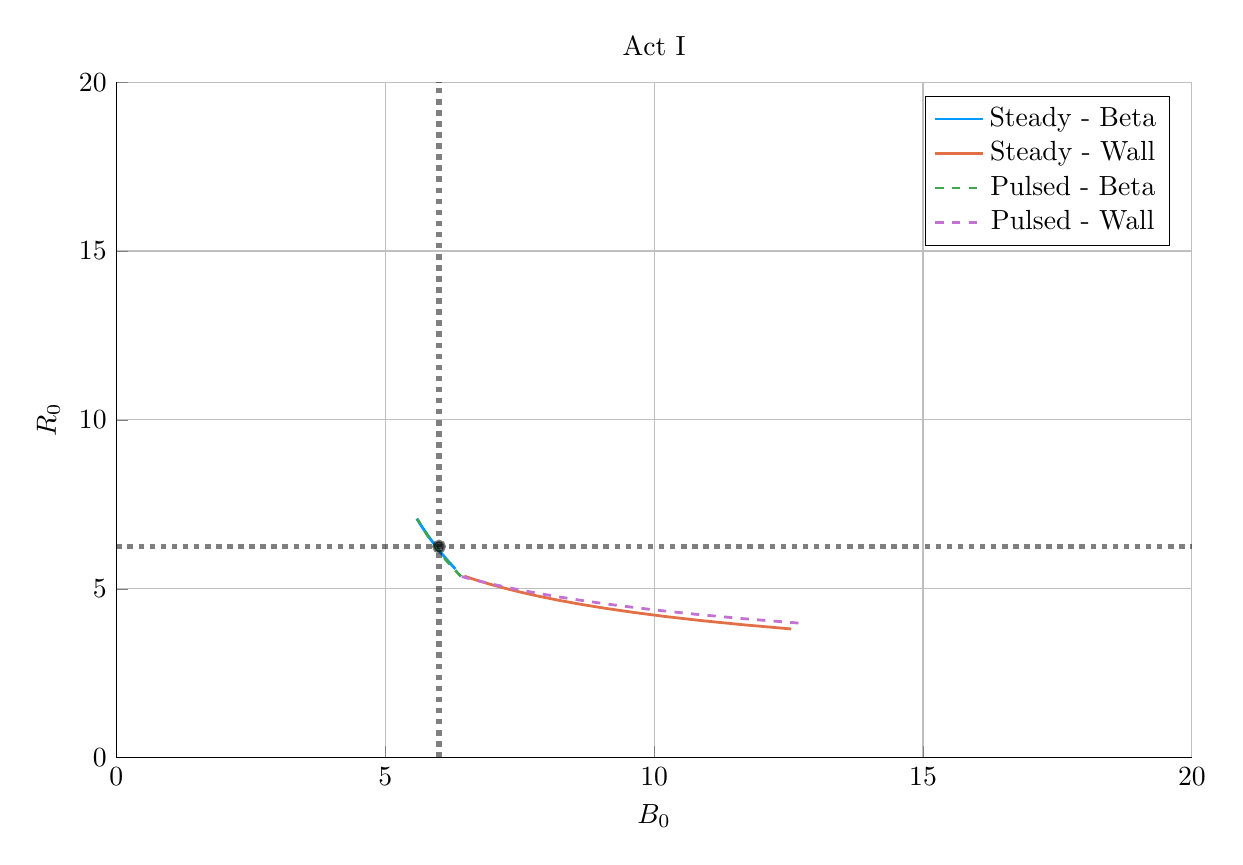
\begin{tikzpicture}[]
\begin{axis}[height = {101.6mm}, ylabel = {${R}_{0}$}, title = {Act I}, xmin = {0.0}, xmax = {20.0}, ymax = {20.0}, xlabel = {${B}_{0}$}, {unbounded coords=jump, scaled x ticks = false, xticklabel style={rotate = 0}, xmajorgrids = true, xtick = {0.0,5.0,10.0,15.0,20.0}, xticklabels = {0,5,10,15,20}, xtick align = inside, axis lines* = left, scaled y ticks = false, yticklabel style={rotate = 0}, ymajorgrids = true, ytick = {0.0,5.0,10.0,15.0,20.0}, yticklabels = {0,5,10,15,20}, ytick align = inside, axis lines* = left,     xshift = 0.0mm,
    yshift = 0.0mm,
    axis background/.style={fill={rgb,1:red,1.00000000;green,1.00000000;blue,1.00000000}}
, colorbar style={title=}}, ymin = {0.0}, width = {152.4mm}]\addplot+ [color = {rgb,1:red,0.00000000;green,0.60560316;blue,0.97868012},
draw opacity=1.0,
line width=1,
solid,mark = none,
mark size = 2.0,
mark options = {
    color = {rgb,1:red,0.00000000;green,0.00000000;blue,0.00000000}, draw opacity = 1.0,
    fill = {rgb,1:red,0.00000000;green,0.60560316;blue,0.97868012}, fill opacity = 1.0,
    line width = 1,
    rotate = 0,
    solid
}]coordinates {
(6.30336807958207, 5.587199391496101)
(6.162193069273141, 5.831838137107903)
(6.030717178404645, 6.078157823726375)
(5.908065509576601, 6.325994353145188)
(5.793464904530972, 6.57518910191267)
(5.686229631357383, 6.825588847053452)
(5.585749511271037, 7.077045564754442)
};
\addlegendentry{Steady - Beta}
\addplot+ [color = {rgb,1:red,0.88887350;green,0.43564919;blue,0.27812294},
draw opacity=1.0,
line width=1,
solid,mark = none,
mark size = 2.0,
mark options = {
    color = {rgb,1:red,0.00000000;green,0.00000000;blue,0.00000000}, draw opacity = 1.0,
    fill = {rgb,1:red,0.88887350;green,0.43564919;blue,0.27812294}, fill opacity = 1.0,
    line width = 1,
    rotate = 0,
    solid
}]coordinates {
(12.549536249695134, 3.8108352245940957)
(11.658754653696462, 3.934083270736017)
(10.883719833507003, 4.057046546594516)
(10.206258129789394, 4.179626810883221)
(9.611335769312953, 4.301750356443285)
(9.086446934250878, 4.423366229113912)
(8.62129895070743, 4.544434218016914)
(8.207216040989662, 4.6649335402400025)
(7.837119555085499, 4.78484200403474)
(7.505047858717157, 4.9041467319817595)
(7.20604322925957, 5.022835870779136)
(6.935884710193303, 5.1409045607718795)
(6.691016583192173, 5.258349129805506)
(6.468415485086983, 5.375167957409874)
};
\addlegendentry{Steady - Wall}
\addplot+ [color = {rgb,1:red,0.24222430;green,0.64327509;blue,0.30444865},
draw opacity=1.0,
line width=1,
dashed,mark = none,
mark size = 2.0,
mark options = {
    color = {rgb,1:red,0.00000000;green,0.00000000;blue,0.00000000}, draw opacity = 1.0,
    fill = {rgb,1:red,0.24222430;green,0.64327509;blue,0.30444865}, fill opacity = 1.0,
    line width = 1,
    rotate = 0,
    solid
}]coordinates {
(6.408263337806559, 5.366131328829866)
(6.408263337806564, 5.366131328829862)
(6.385466513301022, 5.402805883604879)
(6.245492502072912, 5.638974714472524)
(6.116010320461132, 5.875875066688821)
(5.9960421481916395, 6.113307727774442)
(5.884727159112828, 6.351082733498888)
(5.781304768121868, 6.589019058920955)
(5.685100648450046, 6.826944315253105)
(5.595515000321003, 7.064694456596427)
};
\addlegendentry{Pulsed - Beta}
\addplot+ [color = {rgb,1:red,0.76444018;green,0.44411178;blue,0.82429754},
draw opacity=1.0,
line width=1,
dashed,mark = none,
mark size = 2.0,
mark options = {
    color = {rgb,1:red,0.00000000;green,0.00000000;blue,0.00000000}, draw opacity = 1.0,
    fill = {rgb,1:red,0.76444018;green,0.44411178;blue,0.82429754}, fill opacity = 1.0,
    line width = 1,
    rotate = 0,
    solid
}]coordinates {
(12.684248532650473, 3.9847907768802657)
(11.66307871570063, 4.114684512780648)
(10.781888309639141, 4.244124103742294)
(10.016282491385791, 4.373086052625054)
(9.346943280276514, 4.501549309887817)
(8.758420158941194, 4.6294950281779785)
(8.238241792953433, 4.756906348757686)
(7.776255600865612, 4.883768212546736)
(7.364131118520045, 5.010067192354689)
(6.994982564641668, 5.135791343697217)
(6.66307916140573, 5.260930071474144)
(6.408263337806559, 5.366131328829866)
(6.408263337806564, 5.366131328829862)
};
\addlegendentry{Pulsed - Wall}
\addplot+ [color = {rgb,1:red,0.00000000;green,0.00000000;blue,0.00000000},
draw opacity=0.5,
line width=2,
dotted,mark = none,
mark size = 2.0,
mark options = {
    color = {rgb,1:red,0.00000000;green,0.00000000;blue,0.00000000}, draw opacity = 0.5,
    fill = {rgb,1:red,0.00000000;green,0.00000000;blue,0.00000000}, fill opacity = 0.5,
    line width = 1,
    rotate = 0,
    solid
},forget plot]coordinates {
(0.0, 6.25)
(20.0, 6.25)
};
\addplot+ [color = {rgb,1:red,0.00000000;green,0.00000000;blue,0.00000000},
draw opacity=0.5,
line width=2,
dotted,mark = none,
mark size = 2.0,
mark options = {
    color = {rgb,1:red,0.00000000;green,0.00000000;blue,0.00000000}, draw opacity = 0.5,
    fill = {rgb,1:red,0.00000000;green,0.00000000;blue,0.00000000}, fill opacity = 0.5,
    line width = 1,
    rotate = 0,
    solid
},forget plot]coordinates {
(6.0, 0.0)
(6.0, 20.0)
};
\addplot+[draw=none, color = {rgb,1:red,0.00000000;green,0.00000000;blue,0.00000000},
draw opacity=0.5,
line width=0,
solid,mark = *,
mark size = 2.0,
mark options = {
    color = {rgb,1:red,0.00000000;green,0.00000000;blue,0.00000000}, draw opacity = 0.5,
    fill = {rgb,1:red,0.00000000;green,0.00000000;blue,0.00000000}, fill opacity = 0.5,
    line width = 1,
    rotate = 0,
    solid
},forget plot] coordinates {
(6.0, 6.25)
};
\end{axis}

\end{tikzpicture}

    \end{adjustbox}
        \caption{$R_0$ vs $B_0$}
    \end{subfigure}
    \hfill
    \begin{subfigure}[t]{0.45\textwidth}
        \centering
    \begin{adjustbox}{width=\textwidth}
      \Large
      \input{images/comparisons/act_1_I_P_vs_T_bar}
    \end{adjustbox}
        \caption{$I_P$ vs $\overline T$}
    \end{subfigure}
    \hfill \hfill ~\\ ~\\ ~\\
    \caption{ARIES ACT I Model Comparison} ~\\
    \label{fig:act_1_comparison}
\end{figure*}

\begin{table}[b!]
\centering
\caption{ACT I Variables}
\hfill
\begin{subtable}[t]{0.4\textwidth}
\centering
\caption{Input Variables} ~\\
\begin{tabular}{ c|c }

Input            & Value           \\
\hline
$H$              & 1.65            \\
$Q$              & 42.5            \\
$N_{G}$          & 1.0             \\
$\varepsilon$       & 0.25            \\
$\kappa_{95}$    & 2.1             \\
$\delta_{95}$    & 0.4             \\
$\nu_{n}$        & 0.27            \\
$\nu_{T}$        & 1.15            \\
$l_{i}$          & 0.359         \\
$A$              & 2.5             \\
$Z_{eff}$        & 2.11            \\
$f_{D}$          & 0.75            \\
$\tau_{FT}$      & 1.6e9           \\
$B_{CS}$         & 12.77           \\

\end{tabular}
\end{subtable}
\hfill
\begin{subtable}[t]{0.5\textwidth}
\centering
\caption{Output Variables} ~\\
\begin{tabular}{ c|c|c }

Output           & Original         & Fussy.jl        \\
\hline
$R_{0}$          & 6.25             & 6.23           \\
$B_{0}$          & 6.0              & 6.0           \\
$I_{P}$          & 10.95            & 10.78           \\
$\overline n$    & 1.3              & 1.3           \\
$\overline T$    & 20.6             & 17.2            \\
$\beta_{N}$       & 0.0427           & -          \\
$q_{95}$         & 4.5              & 4.0           \\
$P_{W}$          & 2.45             & 2.00           \\
$f_{BS}$         & 0.91             & 0.91           \\
$f_{CD}$         & 0.09             & 0.09           \\
$f_{ID}$         & -              & -             \\
$\volume$         & 582.0            & 621.4           \\
$P_{F}$          & 1813           & 1865          \\
$\eta_{CD}$      & 0.188            & 0.185          \\

\end{tabular}
\end{subtable}
\hfill
\hfill
\label{table:act_1}
\end{table}

\begin{figure*}[t!]
    \centering
    \hfill
    \begin{subfigure}[t]{0.45\textwidth}
        \centering
    \begin{adjustbox}{width=\textwidth}
      \Large
      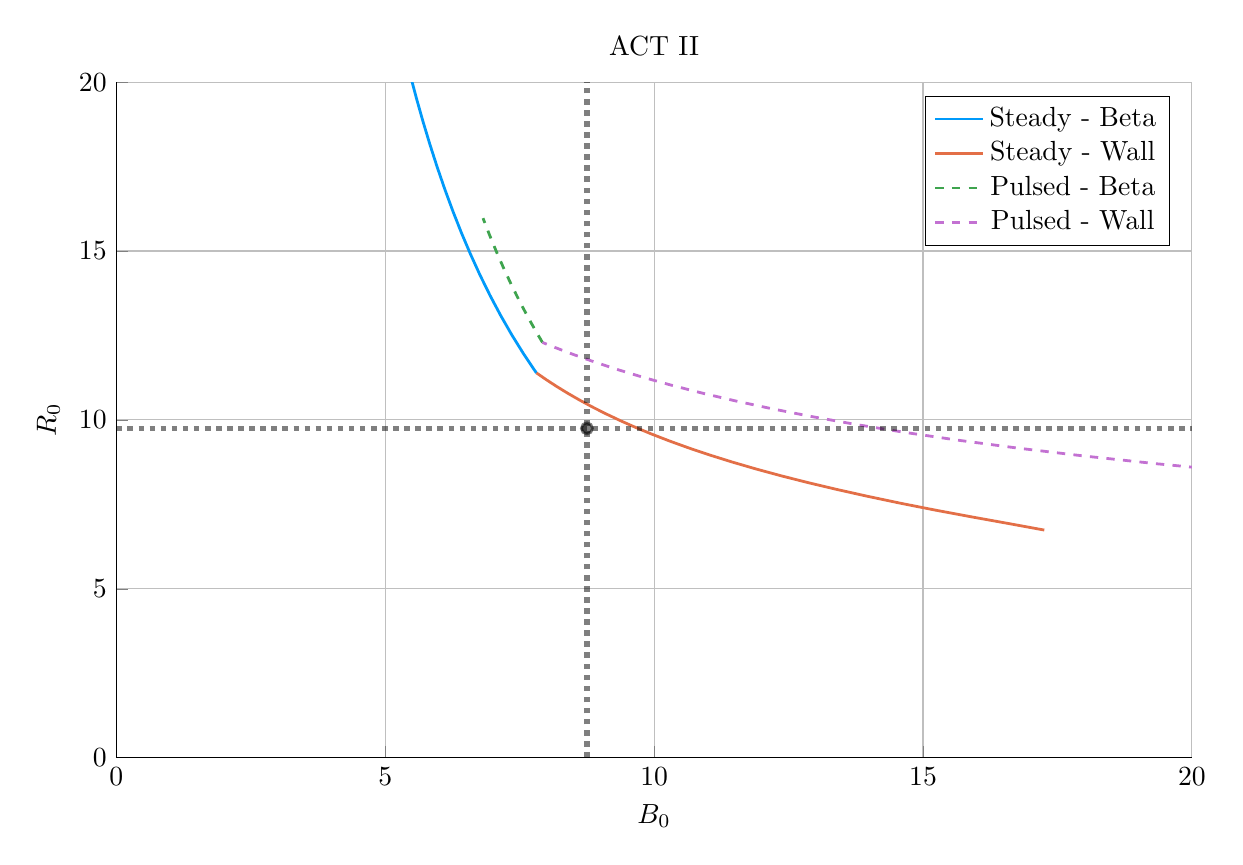
\begin{tikzpicture}[]
\begin{axis}[height = {101.6mm}, ylabel = {${R}_{0}$}, title = {ACT II}, xmin = {0.0}, xmax = {20.0}, ymax = {20.0}, xlabel = {${B}_{0}$}, {unbounded coords=jump, scaled x ticks = false, xticklabel style={rotate = 0}, xmajorgrids = true, xtick = {0.0,5.0,10.0,15.0,20.0}, xticklabels = {0,5,10,15,20}, xtick align = inside, axis lines* = left, scaled y ticks = false, yticklabel style={rotate = 0}, ymajorgrids = true, ytick = {0.0,5.0,10.0,15.0,20.0}, yticklabels = {0,5,10,15,20}, ytick align = inside, axis lines* = left,     xshift = 0.0mm,
    yshift = 0.0mm,
    axis background/.style={fill={rgb,1:red,1.00000000;green,1.00000000;blue,1.00000000}}
, colorbar style={title=}}, ymin = {0.0}, width = {152.4mm}]\addplot+ [color = {rgb,1:red,0.00000000;green,0.60560316;blue,0.97868012},
draw opacity=1.0,
line width=1,
solid,mark = none,
mark size = 2.0,
mark options = {
    color = {rgb,1:red,0.00000000;green,0.00000000;blue,0.00000000}, draw opacity = 1.0,
    fill = {rgb,1:red,0.00000000;green,0.60560316;blue,0.97868012}, fill opacity = 1.0,
    line width = 1,
    rotate = 0,
    solid
}]coordinates {
(7.810935944285959, 11.389141268081966)
(7.57736049850867, 11.942634046586162)
(7.354864292609041, 12.51245847357923)
(7.145167234136329, 13.0943365692581)
(6.9473303865083675, 13.687993788149779)
(6.760499508614096, 14.293145886478186)
(6.583897990324067, 14.909495325365516)
(6.416817229618043, 15.536734694045393)
(6.258609820663305, 16.1745467994937)
(6.108683264880386, 16.82260538899235)
(5.966494431410919, 17.480575868750975)
(5.831544666176381, 18.148116014600475)
(5.703375459679132, 18.824876684423757)
(5.581564609582325, 19.510502502077443)
(5.465722802994068, 20.20463254880097)
(5.355490573482678, 20.906901035327614)
(5.25053558682053, 21.616937949657327)
(5.1505502068221745, 22.334369714080776)
(5.0552493196883175, 23.058819802110854)
};
\addlegendentry{Steady - Beta}
\addplot+ [color = {rgb,1:red,0.88887350;green,0.43564919;blue,0.27812294},
draw opacity=1.0,
line width=1,
solid,mark = none,
mark size = 2.0,
mark options = {
    color = {rgb,1:red,0.00000000;green,0.00000000;blue,0.00000000}, draw opacity = 1.0,
    fill = {rgb,1:red,0.88887350;green,0.43564919;blue,0.27812294}, fill opacity = 1.0,
    line width = 1,
    rotate = 0,
    solid
}]coordinates {
(17.25550839059296, 6.738604635617289)
(16.594334962335296, 6.931178286222189)
(15.9071755430688, 7.128187388035985)
(15.233983138507648, 7.327817939330552)
(14.594239858921854, 7.528927553154291)
(13.989673082630297, 7.7312042898700515)
(13.414782495717416, 7.934790159202381)
(12.872659546281994, 8.139273115071695)
(12.364365715508608, 8.344321605506495)
(11.889507953196574, 8.549679244077495)
(11.44685939646348, 8.755144058838903)
(11.034739998180656, 8.960554762148757)
(10.651252523287319, 9.165781242855727)
(10.294428800132035, 9.370717743724994)
(9.962319203963213, 9.57527782549947)
(9.653045819449929, 9.779390564591205)
(9.364832254395445, 9.982997628553138)
(9.096018465506306, 10.186050992034668)
(8.844373144802077, 10.388606525997883)
(8.61055754360846, 10.590345571972314)
(8.391192178573277, 10.791527736428888)
(8.18577947665566, 10.992035979756642)
(7.99323348423048, 11.1918525509058)
(7.812301489248497, 11.391007917726574)
};
\addlegendentry{Steady - Wall}
\addplot+ [color = {rgb,1:red,0.24222430;green,0.64327509;blue,0.30444865},
draw opacity=1.0,
line width=1,
dashed,mark = none,
mark size = 2.0,
mark options = {
    color = {rgb,1:red,0.00000000;green,0.00000000;blue,0.00000000}, draw opacity = 1.0,
    fill = {rgb,1:red,0.24222430;green,0.64327509;blue,0.30444865}, fill opacity = 1.0,
    line width = 1,
    rotate = 0,
    solid
}]coordinates {
(7.923668284887995, 12.293879059492616)
(7.923668284887995, 12.293879059492635)
(7.836759696043437, 12.52591633746021)
(7.6662731560983355, 13.00454403942661)
(7.50499428233835, 13.488375025456907)
(7.35232773269976, 13.977065733125242)
(7.207727224738343, 14.470269937628656)
(7.070690693175276, 14.967639476613451)
(6.940756001029682, 15.46882496625731)
(6.817497143644154, 15.973476480630131)
};
\addlegendentry{Pulsed - Beta}
\addplot+ [color = {rgb,1:red,0.76444018;green,0.44411178;blue,0.82429754},
draw opacity=1.0,
line width=1,
dashed,mark = none,
mark size = 2.0,
mark options = {
    color = {rgb,1:red,0.00000000;green,0.00000000;blue,0.00000000}, draw opacity = 1.0,
    fill = {rgb,1:red,0.76444018;green,0.44411178;blue,0.82429754}, fill opacity = 1.0,
    line width = 1,
    rotate = 0,
    solid
}]coordinates {
(22.56106430311702, 8.239911323116141)
(20.85607192394036, 8.471453471694678)
(19.335265246056654, 8.703260993170346)
(17.974121547130903, 8.935277031603567)
(16.751976718553127, 9.167446093344447)
(15.651329744019142, 9.399714010238458)
(14.65728744097675, 9.632027927077594)
(13.757118584462601, 9.864336290607328)
(12.939893642194303, 10.096588839007167)
(12.196191964860315, 10.328736591776112)
(11.517862472405039, 10.560731839999896)
(10.897827027335556, 10.792528137074703)
(10.329918077124672, 11.02408028901105)
(9.808743940706389, 11.255344346143936)
(9.329576544487265, 11.486277593626015)
(8.888257451278507, 11.716838542453242)
(8.481118883411932, 11.946986920205564)
(8.10491708701527, 12.17668366154026)
(7.923668284887995, 12.293879059492616)
(7.923668284887995, 12.293879059492635)
};
\addlegendentry{Pulsed - Wall}
\addplot+ [color = {rgb,1:red,0.00000000;green,0.00000000;blue,0.00000000},
draw opacity=0.5,
line width=2,
dotted,mark = none,
mark size = 2.0,
mark options = {
    color = {rgb,1:red,0.00000000;green,0.00000000;blue,0.00000000}, draw opacity = 0.5,
    fill = {rgb,1:red,0.00000000;green,0.00000000;blue,0.00000000}, fill opacity = 0.5,
    line width = 1,
    rotate = 0,
    solid
},forget plot]coordinates {
(0.0, 9.75)
(20.0, 9.75)
};
\addplot+ [color = {rgb,1:red,0.00000000;green,0.00000000;blue,0.00000000},
draw opacity=0.5,
line width=2,
dotted,mark = none,
mark size = 2.0,
mark options = {
    color = {rgb,1:red,0.00000000;green,0.00000000;blue,0.00000000}, draw opacity = 0.5,
    fill = {rgb,1:red,0.00000000;green,0.00000000;blue,0.00000000}, fill opacity = 0.5,
    line width = 1,
    rotate = 0,
    solid
},forget plot]coordinates {
(8.75, 0.0)
(8.75, 20.0)
};
\addplot+[draw=none, color = {rgb,1:red,0.00000000;green,0.00000000;blue,0.00000000},
draw opacity=0.5,
line width=0,
solid,mark = *,
mark size = 2.0,
mark options = {
    color = {rgb,1:red,0.00000000;green,0.00000000;blue,0.00000000}, draw opacity = 0.5,
    fill = {rgb,1:red,0.00000000;green,0.00000000;blue,0.00000000}, fill opacity = 0.5,
    line width = 1,
    rotate = 0,
    solid
},forget plot] coordinates {
(8.75, 9.75)
};
\end{axis}

\end{tikzpicture}

    \end{adjustbox}
        \caption{$R_0$ vs $B_0$}
    \end{subfigure}
    \hfill
    \begin{subfigure}[t]{0.45\textwidth}
        \centering
    \begin{adjustbox}{width=\textwidth}
      \Large
      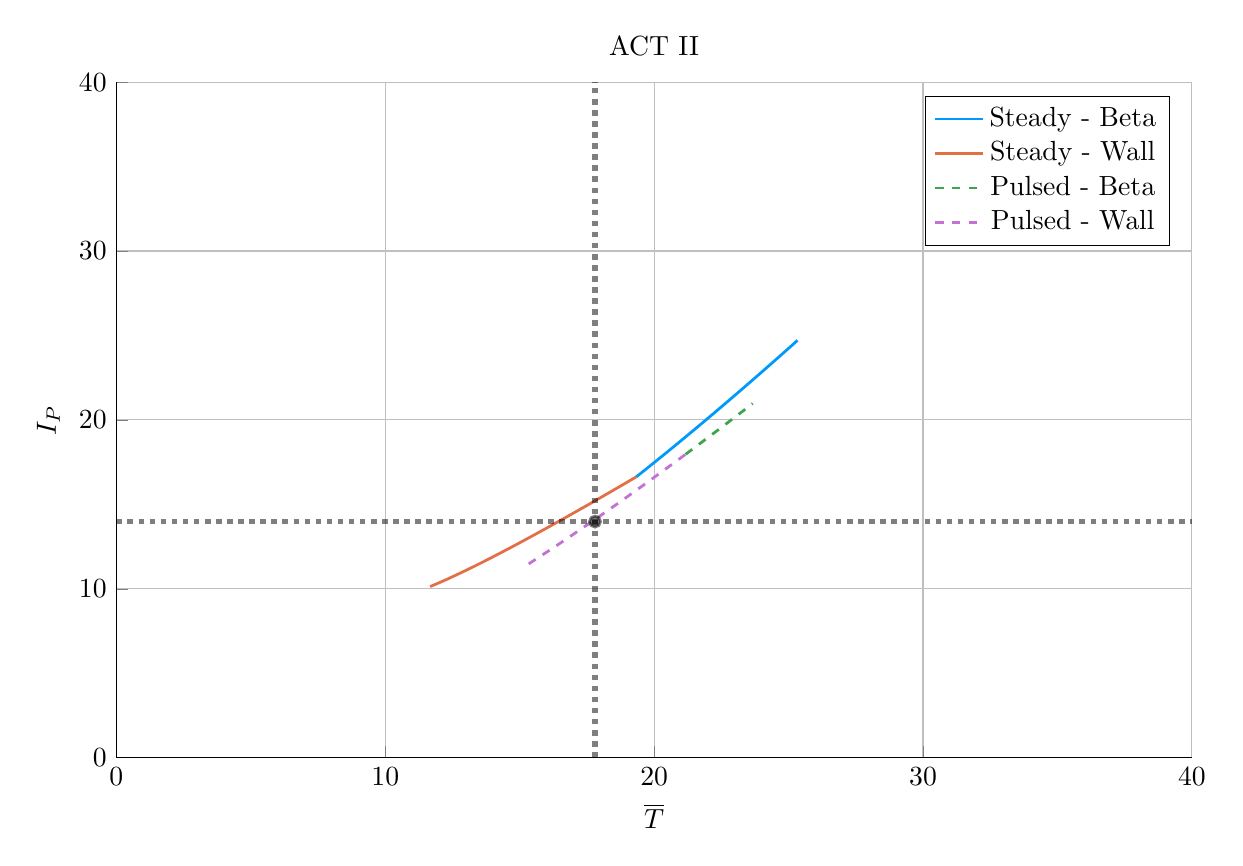
\begin{tikzpicture}[]
\begin{axis}[height = {101.6mm}, ylabel = {${I}_{P}$}, title = {ACT II}, xmin = {0.0}, xmax = {40.0}, ymax = {40.0}, xlabel = {$\overline {T}$}, {unbounded coords=jump, scaled x ticks = false, xticklabel style={rotate = 0}, xmajorgrids = true, xtick = {0.0,10.0,20.0,30.0,40.0}, xticklabels = {0,10,20,30,40}, xtick align = inside, axis lines* = left, scaled y ticks = false, yticklabel style={rotate = 0}, ymajorgrids = true, ytick = {0.0,10.0,20.0,30.0,40.0}, yticklabels = {0,10,20,30,40}, ytick align = inside, axis lines* = left,     xshift = 0.0mm,
    yshift = 0.0mm,
    axis background/.style={fill={rgb,1:red,1.00000000;green,1.00000000;blue,1.00000000}}
, colorbar style={title=}}, ymin = {0.0}, width = {152.4mm}]\addplot+ [color = {rgb,1:red,0.00000000;green,0.60560316;blue,0.97868012},
draw opacity=1.0,
line width=1,
solid,mark = none,
mark size = 2.0,
mark options = {
    color = {rgb,1:red,0.00000000;green,0.00000000;blue,0.00000000}, draw opacity = 1.0,
    fill = {rgb,1:red,0.00000000;green,0.60560316;blue,0.97868012}, fill opacity = 1.0,
    line width = 1,
    rotate = 0,
    solid
}]coordinates {
(19.333333333333332, 16.626976584120992)
(19.666666666666668, 17.04714126565062)
(20.0, 17.4728205159228)
(20.333333333333332, 17.902037802268676)
(20.666666666666668, 18.334710756318135)
(21.0, 18.770758343299946)
(21.333333333333332, 19.21009903030823)
(21.666666666666668, 19.652652028291016)
(22.0, 20.098337062332053)
(22.333333333333332, 20.547074418426956)
(22.666666666666668, 20.998784986741654)
(23.0, 21.453390301179443)
(23.333333333333332, 21.910812577709113)
(23.666666666666668, 22.37097474604109)
(24.0, 22.833800482195542)
(24.333333333333332, 23.299214237115898)
(24.666666666666668, 23.767141260842724)
(25.0, 24.237507628970306)
(25.333333333333332, 24.710240262329886)
};
\addlegendentry{Steady - Beta}
\addplot+ [color = {rgb,1:red,0.88887350;green,0.43564919;blue,0.27812294},
draw opacity=1.0,
line width=1,
solid,mark = none,
mark size = 2.0,
mark options = {
    color = {rgb,1:red,0.00000000;green,0.00000000;blue,0.00000000}, draw opacity = 1.0,
    fill = {rgb,1:red,0.88887350;green,0.43564919;blue,0.27812294}, fill opacity = 1.0,
    line width = 1,
    rotate = 0,
    solid
}]coordinates {
(11.666666666666666, 10.131702672149428)
(12.0, 10.354462623384137)
(12.333333333333334, 10.591104956642406)
(12.666666666666666, 10.837356598740662)
(13.0, 11.09054386610192)
(13.333333333333334, 11.349883742416331)
(13.666666666666666, 11.61561327802365)
(14.0, 11.886764241828663)
(14.333333333333334, 12.16256217004895)
(14.666666666666666, 12.44240841774136)
(15.0, 12.72583049098312)
(15.333333333333334, 13.012449288635679)
(15.666666666666666, 13.301956539143166)
(16.0, 13.59409872387861)
(16.333333333333332, 13.888665310111481)
(16.666666666666668, 14.185479949266789)
(17.0, 14.48439377498311)
(17.333333333333332, 14.785280223642218)
(17.666666666666668, 15.088238807947413)
(18.0, 15.392552774473998)
(18.333333333333332, 15.698764813772398)
(18.666666666666668, 16.00659672680533)
(19.0, 16.315986303185774)
(19.333333333333332, 16.626976584120992)
};
\addlegendentry{Steady - Wall}
\addplot+ [color = {rgb,1:red,0.24222430;green,0.64327509;blue,0.30444865},
draw opacity=1.0,
line width=1,
dashed,mark = none,
mark size = 2.0,
mark options = {
    color = {rgb,1:red,0.00000000;green,0.00000000;blue,0.00000000}, draw opacity = 1.0,
    fill = {rgb,1:red,0.24222430;green,0.64327509;blue,0.30444865}, fill opacity = 1.0,
    line width = 1,
    rotate = 0,
    solid
}]coordinates {
(21.17034352159018, 17.96627417153032)
(21.170343521590212, 17.966274171530337)
(21.333333333333332, 18.1591936305205)
(21.666666666666668, 18.555297107283753)
(22.0, 18.953426399022014)
(22.333333333333332, 19.353497539767794)
(22.666666666666668, 19.7554274455778)
(23.0, 20.159133974954596)
(23.333333333333332, 20.564535986760628)
(23.666666666666668, 20.971553389451927)
};
\addlegendentry{Pulsed - Beta}
\addplot+ [color = {rgb,1:red,0.76444018;green,0.44411178;blue,0.82429754},
draw opacity=1.0,
line width=1,
dashed,mark = none,
mark size = 2.0,
mark options = {
    color = {rgb,1:red,0.00000000;green,0.00000000;blue,0.00000000}, draw opacity = 1.0,
    fill = {rgb,1:red,0.76444018;green,0.44411178;blue,0.82429754}, fill opacity = 1.0,
    line width = 1,
    rotate = 0,
    solid
}]coordinates {
(15.333333333333334, 11.474678053719876)
(15.666666666666666, 11.819475032994422)
(16.0, 12.167858357397087)
(16.333333333333332, 12.51974460671026)
(16.666666666666668, 12.875049128346197)
(17.0, 13.233686175102404)
(17.333333333333332, 13.595569077154208)
(17.666666666666668, 13.96061040317257)
(18.0, 14.328722110173729)
(18.333333333333332, 14.699815683529526)
(18.666666666666668, 15.073802268415148)
(19.0, 15.450592793824576)
(19.333333333333332, 15.830098089115069)
(19.666666666666668, 16.21222899561205)
(20.0, 16.596896471191773)
(20.333333333333332, 16.984011690059134)
(20.666666666666668, 17.37348613728185)
(21.0, 17.765231698435688)
(21.17034352159018, 17.96627417153032)
(21.170343521590212, 17.966274171530337)
};
\addlegendentry{Pulsed - Wall}
\addplot+ [color = {rgb,1:red,0.00000000;green,0.00000000;blue,0.00000000},
draw opacity=0.5,
line width=2,
dotted,mark = none,
mark size = 2.0,
mark options = {
    color = {rgb,1:red,0.00000000;green,0.00000000;blue,0.00000000}, draw opacity = 0.5,
    fill = {rgb,1:red,0.00000000;green,0.00000000;blue,0.00000000}, fill opacity = 0.5,
    line width = 1,
    rotate = 0,
    solid
},forget plot]coordinates {
(0.0, 13.98)
(40.0, 13.98)
};
\addplot+ [color = {rgb,1:red,0.00000000;green,0.00000000;blue,0.00000000},
draw opacity=0.5,
line width=2,
dotted,mark = none,
mark size = 2.0,
mark options = {
    color = {rgb,1:red,0.00000000;green,0.00000000;blue,0.00000000}, draw opacity = 0.5,
    fill = {rgb,1:red,0.00000000;green,0.00000000;blue,0.00000000}, fill opacity = 0.5,
    line width = 1,
    rotate = 0,
    solid
},forget plot]coordinates {
(17.8, 0.0)
(17.8, 40.0)
};
\addplot+[draw=none, color = {rgb,1:red,0.00000000;green,0.00000000;blue,0.00000000},
draw opacity=0.5,
line width=0,
solid,mark = *,
mark size = 2.0,
mark options = {
    color = {rgb,1:red,0.00000000;green,0.00000000;blue,0.00000000}, draw opacity = 0.5,
    fill = {rgb,1:red,0.00000000;green,0.00000000;blue,0.00000000}, fill opacity = 0.5,
    line width = 1,
    rotate = 0,
    solid
},forget plot] coordinates {
(17.8, 13.98)
};
\end{axis}

\end{tikzpicture}

    \end{adjustbox}
        \caption{$I_P$ vs $\overline T$}
    \end{subfigure}
    \hfill \hfill ~\\ ~\\ ~\\
    \caption{ARIES ACT II Model Comparison} ~\\
    \label{fig:act_2_comparison}
\end{figure*}

\begin{table}[b!]
\centering
\caption{ACT II Variables}
\hfill
\begin{subtable}[t]{0.4\textwidth}
\centering
\caption{Input Variables} ~\\
\begin{tabular}{ c|c }

Input            & Value           \\
\hline
$H$              & 1.22            \\
$Q$              & 25.0            \\
$N_{G}$          & 1.3             \\
$\varepsilon$       & 0.25            \\
$\kappa_{95}$    & 1.964           \\
$\delta_{95}$    & 0.42            \\
$\nu_{n}$        & 0.41            \\
$\nu_{T}$        & 1.15            \\
$l_{i}$          & 0.603         \\
$A$              & 2.5             \\
$Z_{eff}$        & 2.12            \\
$f_{D}$          & 0.74            \\
$\tau_{FT}$      & 1.6e9           \\
$B_{CS}$         & 12.77           \\

\end{tabular}
\end{subtable}
\hfill
\begin{subtable}[t]{0.5\textwidth}
\centering
\caption{Output Variables} ~\\
\begin{tabular}{ c|c|c }

Output           & Original         & Fussy.jl        \\
\hline
$R_{0}$          & 9.75             & 10.22           \\
$B_{0}$          & 8.75             & 9.05           \\
$I_{P}$          & 13.98            & 14.84           \\
$\overline n$    & 0.86             & 0.82          \\
$\overline T$    & 17.8             & 17.4           \\
$\beta_{N}$       & 0.026            & 0.023          \\
$q_{95}$         & 8.0              & 6.6           \\
$P_{W}$          & 1.46             & -            \\
$f_{BS}$         & 0.77             & 0.66           \\
$f_{CD}$         & 0.23             & 0.34           \\
$f_{ID}$         & -              & -             \\
$\volume$         & 2209           & 2559          \\
$P_{F}$          & 2637           & 3460          \\
$\eta_{CD}$      & 0.256            & 0.307           \\

\end{tabular}
\end{subtable}
\hfill
\hfill
\label{table:act_2}
\end{table}

\begin{figure*}[t!]
    \centering
    \hfill
    \begin{subfigure}[t]{0.45\textwidth}
        \centering
    \begin{adjustbox}{width=\textwidth}
      \Large
      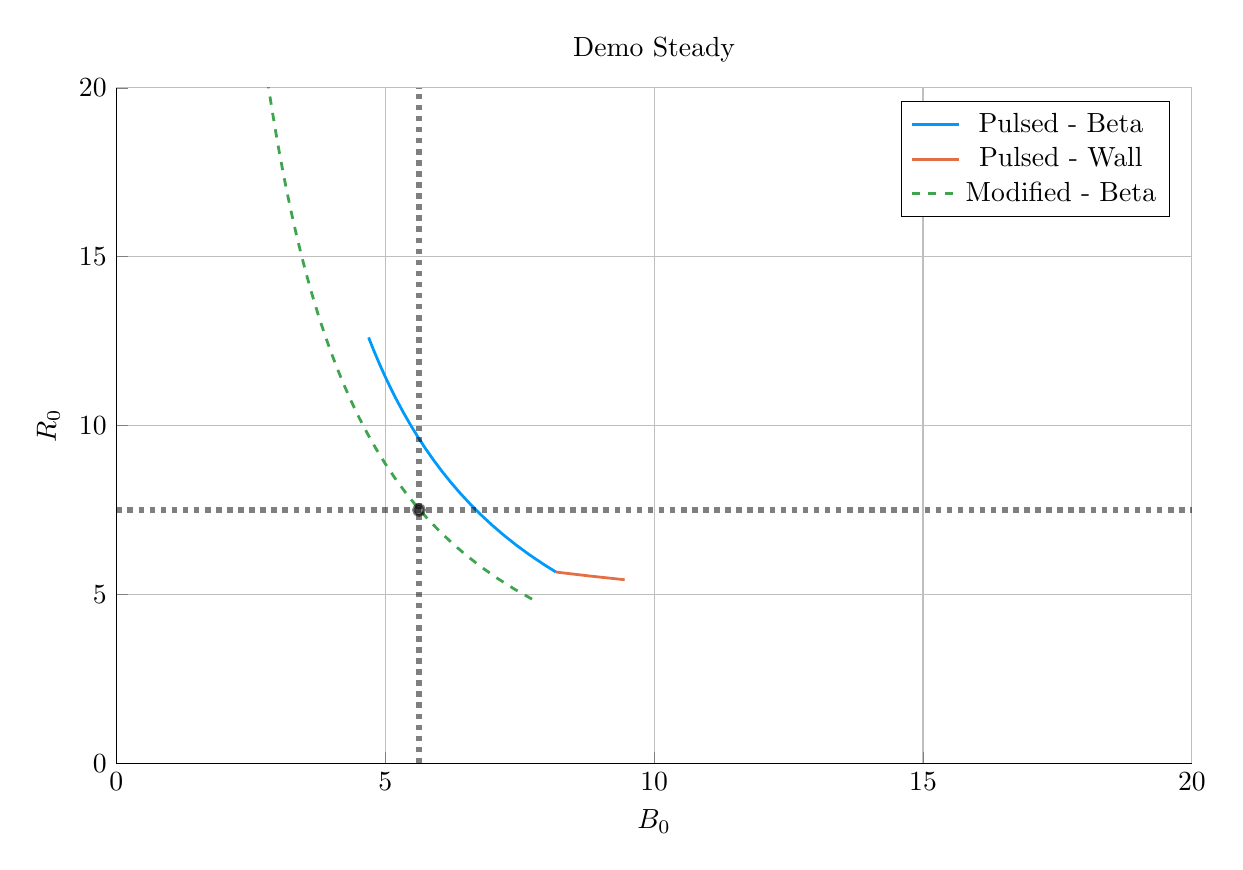
\begin{tikzpicture}[]
\begin{axis}[height = {101.6mm}, ylabel = {${R}_{0}$}, title = {Demo Steady}, xmin = {0.0}, xmax = {20.0}, ymax = {20.0}, xlabel = {${B}_{0}$}, {unbounded coords=jump, scaled x ticks = false, xticklabel style={rotate = 0}, xmajorgrids = true, xtick = {0.0,5.0,10.0,15.0,20.0}, xticklabels = {0,5,10,15,20}, xtick align = inside, axis lines* = left, scaled y ticks = false, yticklabel style={rotate = 0}, ymajorgrids = true, ytick = {0.0,5.0,10.0,15.0,20.0}, yticklabels = {0,5,10,15,20}, ytick align = inside, axis lines* = left,     xshift = 0.0mm,
    yshift = 0.0mm,
    axis background/.style={fill={rgb,1:red,1.00000000;green,1.00000000;blue,1.00000000}}
, colorbar style={title=}}, ymin = {0.0}, width = {152.4mm}]\addplot+ [color = {rgb,1:red,0.00000000;green,0.60560316;blue,0.97868012},
draw opacity=1.0,
line width=1,
solid,mark = none,
mark size = 2.0,
mark options = {
    color = {rgb,1:red,0.00000000;green,0.00000000;blue,0.00000000}, draw opacity = 1.0,
    fill = {rgb,1:red,0.00000000;green,0.60560316;blue,0.97868012}, fill opacity = 1.0,
    line width = 1,
    rotate = 0,
    solid
}]coordinates {
(8.173486873088942, 5.664794455960266)
(7.942780080136996, 5.894389477908349)
(7.682110747013332, 6.174587309854596)
(7.436076373351653, 6.4617259587740365)
(7.203701032854224, 6.7556817964635885)
(6.984087846006315, 7.056316762210614)
(6.776411507024863, 7.363478485110443)
(6.579911624110169, 7.677000456183209)
(6.393886772782909, 7.996702249919802)
(6.217689175869905, 8.322389794615686)
(6.050719935402341, 8.653855690575247)
(5.892424751644716, 8.990879574996331)
(5.742290072962272, 9.333228532083597)
(5.599839627496144, 9.680657546690735)
(5.464631293842628, 10.03290999955685)
(5.33625427328881, 10.389718201981736)
(5.214326530771975, 10.75080396758328)
(5.098492475718857, 11.115879218594692)
(4.98842085737482, 11.484646623994054)
(4.88380285223036, 11.85680026661456)
(4.784350323760147, 12.232026336259217)
(4.689794236961777, 12.610003845742904)
};
\addlegendentry{Pulsed - Beta}
\addplot+ [color = {rgb,1:red,0.88887350;green,0.43564919;blue,0.27812294},
draw opacity=1.0,
line width=1,
solid,mark = none,
mark size = 2.0,
mark options = {
    color = {rgb,1:red,0.00000000;green,0.00000000;blue,0.00000000}, draw opacity = 1.0,
    fill = {rgb,1:red,0.88887350;green,0.43564919;blue,0.27812294}, fill opacity = 1.0,
    line width = 1,
    rotate = 0,
    solid
}]coordinates {
(9.452194760190558, 5.436039445052516)
(8.82895875946862, 5.541751345019407)
(8.260410483462291, 5.64769543408014)
(8.173486873088942, 5.664794455960266)
};
\addlegendentry{Pulsed - Wall}
\addplot+ [color = {rgb,1:red,0.24222430;green,0.64327509;blue,0.30444865},
draw opacity=1.0,
line width=1,
dashed,mark = none,
mark size = 2.0,
mark options = {
    color = {rgb,1:red,0.00000000;green,0.00000000;blue,0.00000000}, draw opacity = 1.0,
    fill = {rgb,1:red,0.24222430;green,0.64327509;blue,0.30444865}, fill opacity = 1.0,
    line width = 1,
    rotate = 0,
    solid
}]coordinates {
(7.729015258613306, 4.861871150043874)
(7.398090906424027, 5.162615732748398)
(7.087604971989989, 5.475689582149146)
(6.796029845186129, 5.801261884855786)
(6.5219747916377235, 6.139486028413868)
(6.264171517105504, 6.490498735804173)
(6.021461495247516, 6.854419238072999)
(5.792784817023639, 7.231348485954994)
(5.57717035299729, 7.621368405021026)
(5.3737270519036775, 8.024541198865679)
(5.1816362256187425, 8.440908704652248)
(5.000144692923053, 8.870491805097014)
(4.828558673035444, 9.313289900712723)
(4.666238335465348, 9.769280445839089)
(4.512592925835539, 10.23841855166636)
(4.367076398389423, 10.720636659108127)
(4.229183495269078, 11.215844284001262)
(4.098446220614958, 11.723927836706606)
(3.974430664327246, 12.244750517759236)
(3.856734136133517, 12.778152290770123)
(3.744982575583214, 13.323949933321568)
(3.6388282078672565, 13.881937166125676)
(3.537947419047361, 14.45188486023713)
(3.4420388274654035, 15.033541321628862)
(3.3508215308612357, 15.626632651963563)
(3.2640335111230074, 16.230863183919308)
(3.18143018067718, 16.84591598897328)
(3.1027830563428513, 17.471453455103656)
(3.0278785480626333, 18.107117931452404)
(2.956516851312625, 18.752532436599008)
(2.888510933213844, 19.407301426734122)
(2.823685603439882, 20.071011619694055)
(2.761876661959762, 20.74323287052923)
(2.702930116488407, 21.423519094029906)
(2.646701463253573, 22.111409229427537)
(2.593055025340143, 22.806428242329144)
};
\addlegendentry{Modified - Beta}
\addplot+ [color = {rgb,1:red,0.00000000;green,0.00000000;blue,0.00000000},
draw opacity=0.5,
line width=2,
dotted,mark = none,
mark size = 2.0,
mark options = {
    color = {rgb,1:red,0.00000000;green,0.00000000;blue,0.00000000}, draw opacity = 0.5,
    fill = {rgb,1:red,0.00000000;green,0.00000000;blue,0.00000000}, fill opacity = 0.5,
    line width = 1,
    rotate = 0,
    solid
},forget plot]coordinates {
(0.0, 7.5)
(20.0, 7.5)
};
\addplot+ [color = {rgb,1:red,0.00000000;green,0.00000000;blue,0.00000000},
draw opacity=0.5,
line width=2,
dotted,mark = none,
mark size = 2.0,
mark options = {
    color = {rgb,1:red,0.00000000;green,0.00000000;blue,0.00000000}, draw opacity = 0.5,
    fill = {rgb,1:red,0.00000000;green,0.00000000;blue,0.00000000}, fill opacity = 0.5,
    line width = 1,
    rotate = 0,
    solid
},forget plot]coordinates {
(5.627, 0.0)
(5.627, 20.0)
};
\addplot+[draw=none, color = {rgb,1:red,0.00000000;green,0.00000000;blue,0.00000000},
draw opacity=0.5,
line width=0,
solid,mark = *,
mark size = 2.0,
mark options = {
    color = {rgb,1:red,0.00000000;green,0.00000000;blue,0.00000000}, draw opacity = 0.5,
    fill = {rgb,1:red,0.00000000;green,0.00000000;blue,0.00000000}, fill opacity = 0.5,
    line width = 1,
    rotate = 0,
    solid
},forget plot] coordinates {
(5.627, 7.5)
};
\end{axis}

\end{tikzpicture}

    \end{adjustbox}
        \caption{$R_0$ vs $B_0$}
    \end{subfigure}
    \hfill
    \begin{subfigure}[t]{0.45\textwidth}
        \centering
    \begin{adjustbox}{width=\textwidth}
      \Large
      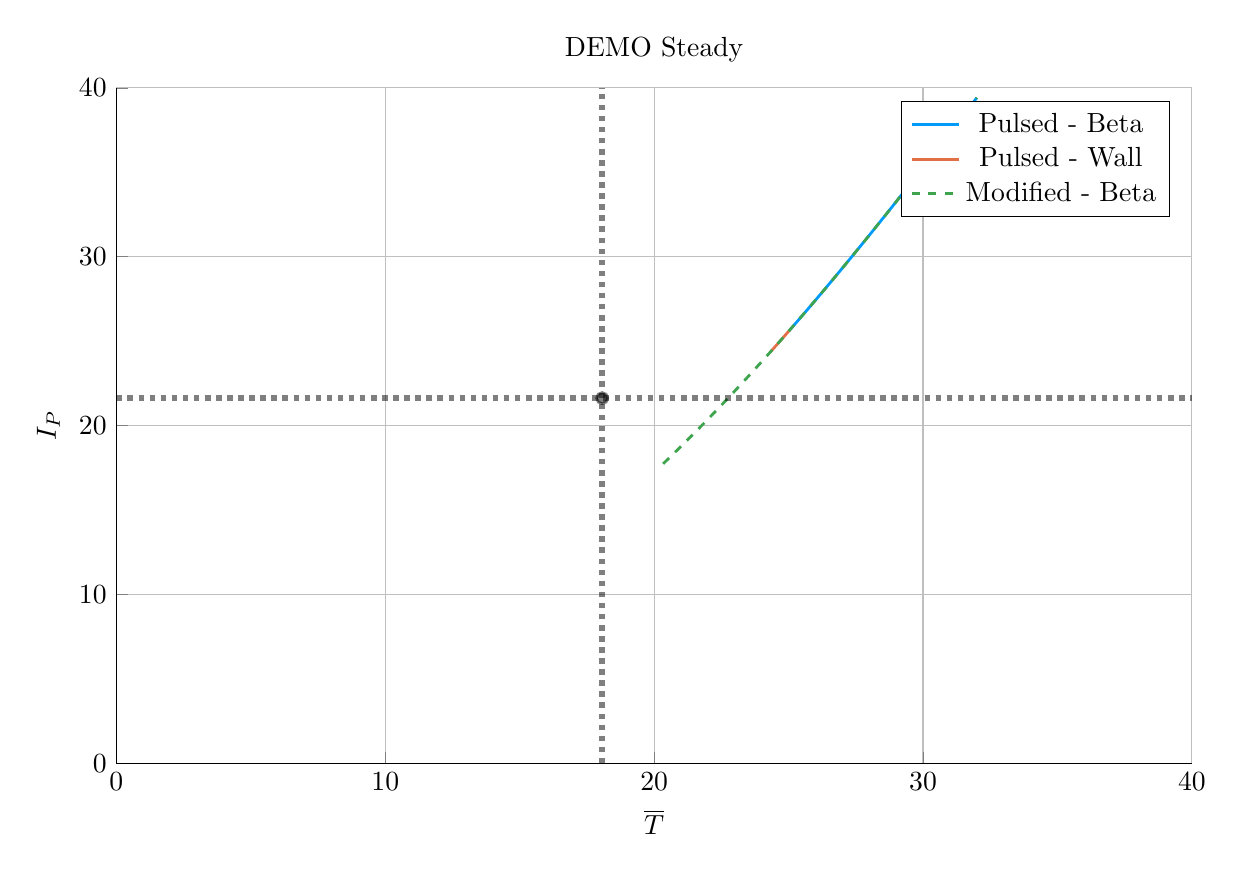
\begin{tikzpicture}[]
\begin{axis}[height = {101.6mm}, ylabel = {${I}_{P}$}, title = {DEMO Steady}, xmin = {0.0}, xmax = {40.0}, ymax = {40.0}, xlabel = {$\overline {T}$}, {unbounded coords=jump, scaled x ticks = false, xticklabel style={rotate = 0}, xmajorgrids = true, xtick = {0.0,10.0,20.0,30.0,40.0}, xticklabels = {0,10,20,30,40}, xtick align = inside, axis lines* = left, scaled y ticks = false, yticklabel style={rotate = 0}, ymajorgrids = true, ytick = {0.0,10.0,20.0,30.0,40.0}, yticklabels = {0,10,20,30,40}, ytick align = inside, axis lines* = left,     xshift = 0.0mm,
    yshift = 0.0mm,
    axis background/.style={fill={rgb,1:red,1.00000000;green,1.00000000;blue,1.00000000}}
, colorbar style={title=}}, ymin = {0.0}, width = {152.4mm}]\addplot+ [color = {rgb,1:red,0.00000000;green,0.60560316;blue,0.97868012},
draw opacity=1.0,
line width=1,
solid,mark = none,
mark size = 2.0,
mark options = {
    color = {rgb,1:red,0.00000000;green,0.00000000;blue,0.00000000}, draw opacity = 1.0,
    fill = {rgb,1:red,0.00000000;green,0.60560316;blue,0.97868012}, fill opacity = 1.0,
    line width = 1,
    rotate = 0,
    solid
}]coordinates {
(25.053735982163357, 25.677558860299992)
(25.333333333333332, 26.189593064380034)
(25.666666666666668, 26.80548085953921)
(26.0, 27.427148406840605)
(26.333333333333332, 28.054440831282633)
(26.666666666666668, 28.68719962041386)
(27.0, 29.325262818659787)
(27.333333333333332, 29.968465226287904)
(27.666666666666668, 30.6166386025962)
(28.0, 31.269611872884024)
(28.333333333333332, 31.92721133872904)
(28.666666666666668, 32.589260891064264)
(29.0, 33.25558222552837)
(29.333333333333332, 33.925995059549685)
(29.666666666666668, 34.60031735061725)
(30.0, 35.27836551518855)
(30.333333333333332, 35.95995464768734)
(30.666666666666668, 36.644898739049395)
(31.0, 37.333010894283476)
(31.333333333333332, 38.02410354852819)
(31.666666666666668, 38.717988681099214)
(32.0, 39.41447802704077)
};
\addlegendentry{Pulsed - Beta}
\addplot+ [color = {rgb,1:red,0.88887350;green,0.43564919;blue,0.27812294},
draw opacity=1.0,
line width=1,
solid,mark = none,
mark size = 2.0,
mark options = {
    color = {rgb,1:red,0.00000000;green,0.00000000;blue,0.00000000}, draw opacity = 1.0,
    fill = {rgb,1:red,0.88887350;green,0.43564919;blue,0.27812294}, fill opacity = 1.0,
    line width = 1,
    rotate = 0,
    solid
}]coordinates {
(24.333333333333332, 24.378107374495485)
(24.666666666666668, 24.975762903314084)
(25.0, 25.579637086786484)
(25.053735982163357, 25.677558860299992)
};
\addlegendentry{Pulsed - Wall}
\addplot+ [color = {rgb,1:red,0.24222430;green,0.64327509;blue,0.30444865},
draw opacity=1.0,
line width=1,
dashed,mark = none,
mark size = 2.0,
mark options = {
    color = {rgb,1:red,0.00000000;green,0.00000000;blue,0.00000000}, draw opacity = 1.0,
    fill = {rgb,1:red,0.24222430;green,0.64327509;blue,0.30444865}, fill opacity = 1.0,
    line width = 1,
    rotate = 0,
    solid
}]coordinates {
(20.333333333333332, 17.737142606162497)
(20.666666666666668, 18.250736761644205)
(21.0, 18.771889258341997)
(21.333333333333332, 19.300518519223587)
(21.666666666666668, 19.836537357082282)
(22.0, 20.37985305559639)
(22.333333333333332, 20.930367463801495)
(22.666666666666668, 21.487977099646507)
(23.0, 22.05257326267931)
(23.333333333333332, 22.62404215595106)
(23.666666666666668, 23.202265017123075)
(24.0, 23.787118258664318)
(24.333333333333332, 24.378473616949)
(24.666666666666668, 24.976198309995638)
(25.0, 25.58015520352756)
(25.333333333333332, 26.19020298497985)
(25.666666666666668, 26.806196345025047)
(26.0, 27.427986166140983)
(26.333333333333332, 28.055419717698932)
(26.666666666666668, 28.688340857006587)
(27.0, 29.3265902357016)
(27.333333333333332, 29.970005510854897)
(27.666666666666668, 30.61842156011136)
(28.0, 31.27167070016686)
(28.333333333333332, 31.92958290785876)
(28.666666666666668, 32.591986043126525)
(29.0, 33.25870607308836)
(29.333333333333332, 33.929567296470175)
(29.666666666666668, 34.604392567622554)
(30.0, 35.28300351936469)
(30.333333333333332, 35.96522078390488)
(30.666666666666668, 36.650864211102025)
(31.0, 37.3397530833557)
(31.333333333333332, 38.03170632643894)
(31.666666666666668, 38.726542715621264)
(32.0, 39.424081076468326)
};
\addlegendentry{Modified - Beta}
\addplot+ [color = {rgb,1:red,0.00000000;green,0.00000000;blue,0.00000000},
draw opacity=0.5,
line width=2,
dotted,mark = none,
mark size = 2.0,
mark options = {
    color = {rgb,1:red,0.00000000;green,0.00000000;blue,0.00000000}, draw opacity = 0.5,
    fill = {rgb,1:red,0.00000000;green,0.00000000;blue,0.00000000}, fill opacity = 0.5,
    line width = 1,
    rotate = 0,
    solid
},forget plot]coordinates {
(0.0, 21.627)
(40.0, 21.627)
};
\addplot+ [color = {rgb,1:red,0.00000000;green,0.00000000;blue,0.00000000},
draw opacity=0.5,
line width=2,
dotted,mark = none,
mark size = 2.0,
mark options = {
    color = {rgb,1:red,0.00000000;green,0.00000000;blue,0.00000000}, draw opacity = 0.5,
    fill = {rgb,1:red,0.00000000;green,0.00000000;blue,0.00000000}, fill opacity = 0.5,
    line width = 1,
    rotate = 0,
    solid
},forget plot]coordinates {
(18.067, 0.0)
(18.067, 40.0)
};
\addplot+[draw=none, color = {rgb,1:red,0.00000000;green,0.00000000;blue,0.00000000},
draw opacity=0.5,
line width=0,
solid,mark = *,
mark size = 2.0,
mark options = {
    color = {rgb,1:red,0.00000000;green,0.00000000;blue,0.00000000}, draw opacity = 0.5,
    fill = {rgb,1:red,0.00000000;green,0.00000000;blue,0.00000000}, fill opacity = 0.5,
    line width = 1,
    rotate = 0,
    solid
},forget plot] coordinates {
(18.067, 21.627)
};
\end{axis}

\end{tikzpicture}

    \end{adjustbox}
        \caption{$I_P$ vs $\overline T$}
    \end{subfigure}
    \hfill \hfill ~\\ ~\\ ~\\
    \caption{DEMO Steady Model Comparison} ~\\
    \label{fig:demo_steady_comparison}
\end{figure*}

\begin{table}[b!]
\centering
\caption{DEMO Steady Variables}
\hfill
\begin{subtable}[t]{0.4\textwidth}
\centering
\caption{Input Variables} ~\\
\begin{tabular}{ c|c }

Input            & Value           \\
\hline
$H$              & 1.4             \\
$Q$              & 24.46           \\
$N_{G}$          & 1.2             \\
$\varepsilon$       & 0.385           \\
$\kappa_{95}$    & 1.8             \\
$\delta_{95}$    & 0.333           \\
$\nu_{n}$        & 0.3972          \\
$\nu_{T}$        & 0.9187          \\
$l_{i}$          & 0.900             \\
$A$              & 2.856           \\
$Z_{eff}$        & 4.708           \\
$f_{D}$          & 0.7366          \\
$\tau_{FT}$      & 1.6e9           \\
$B_{CS}$         & 12.85           \\

\end{tabular}
\end{subtable}
\hfill
\begin{subtable}[t]{0.5\textwidth}
\centering
\caption{Output Variables} ~\\
\begin{tabular}{ c|c|c|c }

Output           & Original         & Fussy.jl  & Modified      \\
\hline
$R_{0}$          & 7.5              & 8.2  &  7.6        \\
$B_{0}$          & 5.627            & 6.307  & 5.577         \\
$I_{P}$          & 21.63            & 30.93   &  22.05       \\
$\overline n$    & 0.875           & 1.048   & 0.855        \\
$\overline T$    & 18.07            & 27.83    &  23.00       \\
$\beta_{N}$       & 0.038            & - & -         \\
$q_{95}$         & 4.405            & 3.761 &   4.360         \\
$P_{W}$          & 1.911            & 4.151 &    2.281       \\
$f_{BS}$         & 0.611            & 0.424  &  0.492       \\
$f_{CD}$         & 0.389            & 0.576 &  0.508        \\
$f_{ID}$         & -              & -             & - \\
$\volume$         & 2217           & 2879 &  2351        \\
$P_{F}$          & 3255           & 8971 & 4306         \\
$\eta_{CD}$      & 0.4152           & -  & -        \\

\end{tabular}
\end{subtable}
\hfill
\hfill
\label{table:demo_steady}
\end{table}

\begin{figure*}[t!]
    \centering
    \hfill
    \begin{subfigure}[t]{0.45\textwidth}
        \centering
    \begin{adjustbox}{width=\textwidth}
      \Large
      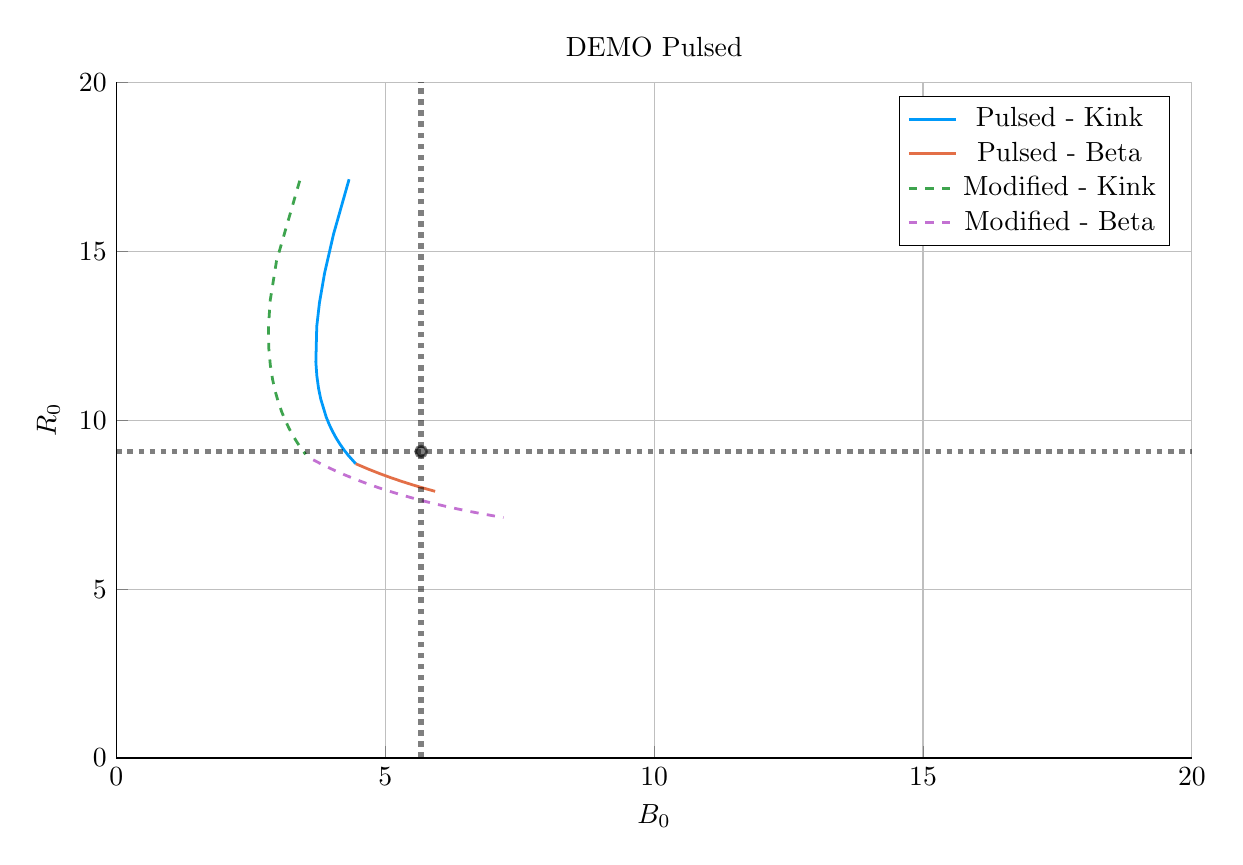
\begin{tikzpicture}[]
\begin{axis}[height = {101.6mm}, ylabel = {${R}_{0}$}, title = {DEMO Pulsed}, xmin = {0.0}, xmax = {20.0}, ymax = {20.0}, xlabel = {${B}_{0}$}, {unbounded coords=jump, scaled x ticks = false, xticklabel style={rotate = 0}, xmajorgrids = true, xtick = {0.0,5.0,10.0,15.0,20.0}, xticklabels = {0,5,10,15,20}, xtick align = inside, axis lines* = left, scaled y ticks = false, yticklabel style={rotate = 0}, ymajorgrids = true, ytick = {0.0,5.0,10.0,15.0,20.0}, yticklabels = {0,5,10,15,20}, ytick align = inside, axis lines* = left,     xshift = 0.0mm,
    yshift = 0.0mm,
    axis background/.style={fill={rgb,1:red,1.00000000;green,1.00000000;blue,1.00000000}}
, colorbar style={title=}}, ymin = {0.0}, width = {152.4mm}]\addplot+ [color = {rgb,1:red,0.00000000;green,0.60560316;blue,0.97868012},
draw opacity=1.0,
line width=1,
solid,mark = none,
mark size = 2.0,
mark options = {
    color = {rgb,1:red,0.00000000;green,0.00000000;blue,0.00000000}, draw opacity = 1.0,
    fill = {rgb,1:red,0.00000000;green,0.60560316;blue,0.97868012}, fill opacity = 1.0,
    line width = 1,
    rotate = 0,
    solid
}]coordinates {
(4.327031075670194, 17.134796748649162)
(4.038214026054326, 15.511755022601415)
(3.8713719163129245, 14.355562963913712)
(3.7758613845615545, 13.476675762289453)
(3.7257856761317214, 12.778294295391971)
(3.7090473695925437, 11.723065749829066)
(3.727711597554826, 11.30970201784727)
(3.7586131667481433, 10.94971275897184)
(3.799052518631718, 10.632190690377048)
(3.901290136389271, 10.09455415135144)
(3.960577465316514, 9.863813619410237)
(4.0241209645210345, 9.653307397969705)
(4.0912717805663785, 9.460162902699798)
(4.161514602943343, 9.28206292757184)
(4.2344343960723005, 9.117114543572253)
(4.309692554546368, 8.963753917462126)
(4.450417240491067, 8.712493965092264)
};
\addlegendentry{Pulsed - Kink}
\addplot+ [color = {rgb,1:red,0.88887350;green,0.43564919;blue,0.27812294},
draw opacity=1.0,
line width=1,
solid,mark = none,
mark size = 2.0,
mark options = {
    color = {rgb,1:red,0.00000000;green,0.00000000;blue,0.00000000}, draw opacity = 1.0,
    fill = {rgb,1:red,0.88887350;green,0.43564919;blue,0.27812294}, fill opacity = 1.0,
    line width = 1,
    rotate = 0,
    solid
}]coordinates {
(4.450417240491067, 8.712493965092264)
(4.490148631384312, 8.684308742646298)
(4.692490181445514, 8.547262773806349)
(4.8960344619053355, 8.41947837460442)
(5.100651132702229, 8.30014929484307)
(5.306202822090688, 8.188581738801314)
(5.512545696627038, 8.084175191078112)
(5.719530043226767, 7.986407002697611)
(5.927000883375481, 7.894819882619234)
};
\addlegendentry{Pulsed - Beta}
\addplot+ [color = {rgb,1:red,0.24222430;green,0.64327509;blue,0.30444865},
draw opacity=1.0,
line width=1,
dashed,mark = none,
mark size = 2.0,
mark options = {
    color = {rgb,1:red,0.00000000;green,0.00000000;blue,0.00000000}, draw opacity = 1.0,
    fill = {rgb,1:red,0.24222430;green,0.64327509;blue,0.30444865}, fill opacity = 1.0,
    line width = 1,
    rotate = 0,
    solid
}]coordinates {
(3.4087424183072135, 17.090884129081292)
(2.977074181068944, 14.713048632784332)
(2.8592500074202523, 13.541171522519205)
(2.827199220063259, 12.740024138753894)
(2.8339789008667826, 12.12574468151967)
(2.862412302880871, 11.626187613249266)
(2.9044598258085443, 11.205091848948229)
(2.95577893007882, 10.841432203317366)
(3.0137895352525907, 10.521822649209419)
(3.076849710218805, 10.23716073884787)
(3.1438583711612704, 9.980947801083442)
(3.214045733980633, 9.748367275345563)
(3.2868548955983727, 9.535742205343247)
(3.361871149981842, 9.340197658526863)
(3.4387778750377818, 9.15944098345979)
(3.5173279629378453, 8.991613349767409)
};
\addlegendentry{Modified - Kink}
\addplot+ [color = {rgb,1:red,0.76444018;green,0.44411178;blue,0.82429754},
draw opacity=1.0,
line width=1,
dashed,mark = none,
mark size = 2.0,
mark options = {
    color = {rgb,1:red,0.00000000;green,0.00000000;blue,0.00000000}, draw opacity = 1.0,
    fill = {rgb,1:red,0.76444018;green,0.44411178;blue,0.82429754}, fill opacity = 1.0,
    line width = 1,
    rotate = 0,
    solid
}]coordinates {
(3.6607028750648505, 8.825949645171955)
(3.8574448036470477, 8.664618827122876)
(4.056375867871351, 8.51434867582932)
(4.257366397480293, 8.374075613831488)
(4.460279103534801, 8.242896218794312)
(4.664969389370631, 8.12003771613466)
(4.871285596007394, 8.004834914067093)
(5.07906923307514, 7.896711937521184)
(5.288155233306219, 7.795167587687744)
(5.498372259673351, 7.699763475973523)
(5.709543087166185, 7.610114306522102)
(5.921485076209294, 7.525879840414137)
(6.134010749367255, 7.446758190646709)
(6.346928478632384, 7.372480180910637)
(6.560043285872518, 7.302804563889649)
(6.773157754368795, 7.237513941672651)
(6.986073044284746, 7.176411266758267)
(7.198590001107076, 7.119316828230052)
};
\addlegendentry{Modified - Beta}
\addplot+ [color = {rgb,1:red,0.00000000;green,0.00000000;blue,0.00000000},
draw opacity=0.5,
line width=2,
dotted,mark = none,
mark size = 2.0,
mark options = {
    color = {rgb,1:red,0.00000000;green,0.00000000;blue,0.00000000}, draw opacity = 0.5,
    fill = {rgb,1:red,0.00000000;green,0.00000000;blue,0.00000000}, fill opacity = 0.5,
    line width = 1,
    rotate = 0,
    solid
},forget plot]coordinates {
(0.0, 9.072)
(20.0, 9.072)
};
\addplot+ [color = {rgb,1:red,0.00000000;green,0.00000000;blue,0.00000000},
draw opacity=0.5,
line width=2,
dotted,mark = none,
mark size = 2.0,
mark options = {
    color = {rgb,1:red,0.00000000;green,0.00000000;blue,0.00000000}, draw opacity = 0.5,
    fill = {rgb,1:red,0.00000000;green,0.00000000;blue,0.00000000}, fill opacity = 0.5,
    line width = 1,
    rotate = 0,
    solid
},forget plot]coordinates {
(5.667, 0.0)
(5.667, 20.0)
};
\addplot+[draw=none, color = {rgb,1:red,0.00000000;green,0.00000000;blue,0.00000000},
draw opacity=0.5,
line width=0,
solid,mark = *,
mark size = 2.0,
mark options = {
    color = {rgb,1:red,0.00000000;green,0.00000000;blue,0.00000000}, draw opacity = 0.5,
    fill = {rgb,1:red,0.00000000;green,0.00000000;blue,0.00000000}, fill opacity = 0.5,
    line width = 1,
    rotate = 0,
    solid
},forget plot] coordinates {
(5.667, 9.072)
};
\end{axis}

\end{tikzpicture}

    \end{adjustbox}
        \caption{$R_0$ vs $B_0$}
    \end{subfigure}
    \hfill
    \begin{subfigure}[t]{0.45\textwidth}
        \centering
    \begin{adjustbox}{width=\textwidth}
      \Large
      \input{images/comparisons/demo_pulsed_I_P_vs_T_bar}
    \end{adjustbox}
        \caption{$I_P$ vs $\overline T$}
    \end{subfigure}
    \hfill \hfill ~\\ ~\\ ~\\
    \caption{DEMO Pulsed Model Comparison} ~\\
    \label{fig:demo_pulsed_comparison}
\end{figure*}

\begin{table}[b!]
\centering
\caption{DEMO Pulsed Variables}
\hfill
\begin{subtable}[t]{0.4\textwidth}
\centering
\caption{Input Variables} ~\\
\begin{tabular}{ c|c }

Input            & Value           \\
\hline
$H$              & 1.1             \\
$Q$              & 39.86           \\
$N_{G}$          & 1.2             \\
$\varepsilon$       & 0.3226          \\
$\kappa_{95}$    & 1.59            \\
$\delta_{95}$    & 0.333           \\
$\nu_{n}$        & 0.27            \\
$\nu_{T}$        & 1.094           \\
$l_{i}$          & 1.155           \\
$A$              & 2.735           \\
$Z_{eff}$        & 2.584           \\
$f_{D}$          & 0.7753          \\
$\tau_{FT}$      & 7273          \\
$B_{CS}$         & 12.77           \\

\end{tabular}
\end{subtable}
\hfill
\begin{subtable}[t]{0.5\textwidth}
\centering
\caption{Output Variables} ~\\
\begin{tabular}{ c|c|c|c }

Output           & Original         & Fussy.jl  & Modified      \\
\hline
$R_{0}$          & 9.07            & 8.10   & 7.61           \\
$B_{0}$          & 5.67            & 5.48   &  5.71        \\
$I_{P}$          & 19.6             & 19.3 &   16.3       \\
$\overline n$    & 0.7983           & 0.9795 &   0.9384      \\
$\overline T$    & 13.06            & 13.28 & 13.00         \\
$\beta_{N}$       & 0.0259           & - & -         \\
$q_{95}$         & 3.247            & 2.853 & 3.303          \\
$P_{W}$          & 1.05             & 1.47 & 1.23          \\
$f_{BS}$         & 0.348            & 0.164 & 0.190         \\
$f_{CD}$         & 0.096            & 0.106 &  0.103        \\
$f_{ID}$         & 0.557            & 0.730  & 0.707         \\
$\volume$         & 2502           & 1751  & 1452        \\
$P_{F}$          & 2037           & 2376 & 1756         \\
$\eta_{CD}$      & 0.2721           & - & -

\end{tabular}
\end{subtable}
\hfill
\hfill
\label{table:demo_pulsed}
\end{table}

\clearpage

\newpage

\section{Developing Prototype Reactors}

Now that the model used in Fussy.jl has been tested against other fusion systems codes in the field, we will develop our own prototype reactors. Because this paper is about making a levelized comparison of pulsed and steady-state tokamaks, we will develop middle-of-the-road reactors that only differ by operating mode. \added{The parameters for these two designs are captured in \cref{table:charybdis,table:proteus}.}

\replaced{To compare the two modes of operation, the}{The} steady-state prototype, Charybdis, is the obvious choice to start with -- as the model was tested against four of these typed reactors. It was also pointed out that the model did remarkably well when recreating ARC. As the authors share many of the ARC team's philosophies, Charybdis uses \replaced{static}{fixed} parameters very similar to them.\cite{arc}

Next, although led to believe Charybdis' pulsed twin reactor -- Proteus -- would be created by a simple flip of the switch, it was a slight oversimplification. The first difference is that the pulsed twin, Proteus, is assumed to be purely pulsed: $\eta_{CD} = 0$. Further, the bootstrap current is much less important than it was for steady-state tokamaks. This corresponds to a current profile peaked at the origin -- i.e.\ a parabola. Numerically, this is done by raising $l_i$ from around \replaced{0.55}{5.5} to \replaced{0.6}{6}.

The final difference creates the largest change in the twin reactors: the choice of \replaced{necessary technological advancement.}{miracle.} As \replaced{mentioned}{hinted} several times before, the H factor is a common way designers artificially boost the confinement of their machines. This H value will thus be the \replaced{technological advancement needed}{miracle} for Charybdis, the steady-state prototype. Next, as the main conclusion of this paper is to state the advantages of high magnetic field, \replaced{an inexpensive way to strengthen the}{a free way to boost a} central solenoid of Proteus -- through $B_{CS}$ -- will be employed using HTS coils.

\deleted{Opposite the order of how they were designed, the goal now is to lock down a value of $B_{CS}$ for Proteus and then use it to set the H factor for Charybdis. This selection algorithm is depicted in Fig.\ \ref{fig:selection}. For Proteus, the point locked down was $B_{CS} = 20 \ \textnormal{T}$, which occurred at a fusion power ($P_F$) of around 1250 MW. As shown in the cost curve, this was at a point where the ratio between the minimum capital cost and the minimum cost-per-watt saturated. This choice of a 1250 MW reactor then led to Charybdis having an H factor of 1.7.}

\added{The goal now is to impose a constraint on a reactor's economic competitiveness by setting the fusion power to a relatively low value for both designs -- i.e.\ 1250 MW. As \cref{fig:selection} shows, this results in Charybdis having an H factor of 1.7 and Proteus having a $B_{CS}$ of around 20T. As shown in the Proteus cost curve, this was at a point where the ratio between the minimum capital cost and the minimum cost-per-watt leveled off. }

\added{Note that these technological advancements (in H and $B_{CS}$) are necessary to get economic -- or even physically realizable -- reactors. This is the same reason why all the literature reactors used values for H and $N_G$ that violate standard values.}

\begin{figure}[b!]
\centering
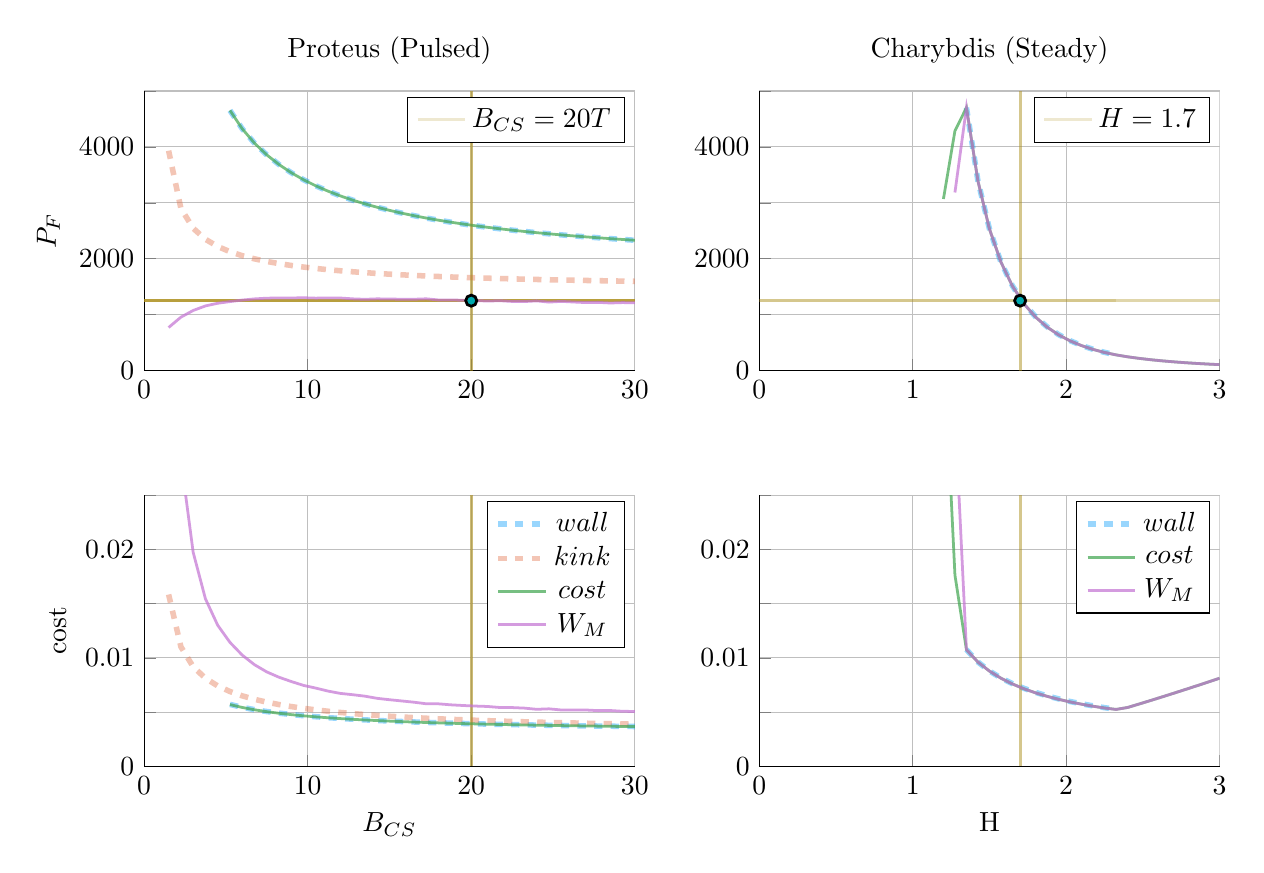
\begin{tikzpicture}[]
\begin{axis}[height = {51.32916666666667mm}, ylabel = {$P_F$}, title = {Proteus (Pulsed)}, xmin = {0}, xmax = {30.0}, ymax = {5000.0}, xlabel = {}, {unbounded coords=jump, scaled x ticks = false, xticklabel style={rotate = 0}, xmajorgrids = true, xtick = {0.0,10.0,20.0,30.0}, xticklabels = {0,10,20,30}, xtick align = inside, axis lines* = left, scaled y ticks = false, yticklabel style={rotate = 0}, ymajorgrids = true, ytick = {0,1000,2000,3000,4000,5000}, yticklabels = {0,,2000,,4000,}, ytick align = inside, axis lines* = left,     xshift = 0.0mm,
    yshift = 50.27mm,
    axis background/.style={fill={rgb,1:red,1.00000000;green,1.00000000;blue,1.00000000}}
}, ymin = {2.220446049250313e-16}, width = {78.14027777777778mm}]\addplot+ [color = {rgb,1:red,0.67554396;green,0.55566233;blue,0.09423434},
draw opacity=0.2,
line width=1,
solid,mark = none,
mark size = 2.0,
mark options = {
    color = {rgb,1:red,0.00000000;green,0.00000000;blue,0.00000000}, draw opacity = 1.0,
    fill = {rgb,1:red,0.67554396;green,0.55566233;blue,0.09423434}, fill opacity = 1.0,
    line width = 1,
    rotate = 0,
    solid
}]coordinates {
(20.0, 2.220446049250313e-16)
(20.0, 5000.0)
};
\addlegendentry{$B_{CS} = 20 T$}
\addplot+ [color = {rgb,1:red,0.67554396;green,0.55566233;blue,0.09423434},
draw opacity=0.2,
line width=1,
solid,mark = none,
mark size = 2.0,
mark options = {
    color = {rgb,1:red,0.00000000;green,0.00000000;blue,0.00000000}, draw opacity = 1.0,
    fill = {rgb,1:red,0.67554396;green,0.55566233;blue,0.09423434}, fill opacity = 1.0,
    line width = 1,
    rotate = 0,
    solid
},forget plot]coordinates {
(0.0, 1250.0)
(30.0, 1250.0)
};
\addplot+[draw=none, color = {rgb,1:red,0.00000048;green,0.66575898;blue,0.68099695},
draw opacity=1.0,
line width=0,
solid,mark = *,
mark size = 2.0,
mark options = {
    color = {rgb,1:red,0.00000000;green,0.00000000;blue,0.00000000}, draw opacity = 1.0,
    fill = {rgb,1:red,0.00000048;green,0.66575898;blue,0.68099695}, fill opacity = 1.0,
    line width = 1,
    rotate = 0,
    solid
},forget plot] coordinates {
(20, 1250)
};
\addplot+ [color = {rgb,1:red,0.67554396;green,0.55566233;blue,0.09423434},
draw opacity=0.2,
line width=1,
solid,mark = none,
mark size = 2.0,
mark options = {
    color = {rgb,1:red,0.00000000;green,0.00000000;blue,0.00000000}, draw opacity = 1.0,
    fill = {rgb,1:red,0.67554396;green,0.55566233;blue,0.09423434}, fill opacity = 1.0,
    line width = 1,
    rotate = 0,
    solid
},forget plot]coordinates {
(0.0, 1250.0)
(30.0, 1250.0)
};
\addplot+ [color = {rgb,1:red,0.00000000;green,0.60560316;blue,0.97868012},
draw opacity=0.4,
line width=2,
dashed,mark = none,
mark size = 2.0,
mark options = {
    color = {rgb,1:red,0.00000000;green,0.00000000;blue,0.00000000}, draw opacity = 1.0,
    fill = {rgb,1:red,0.00000000;green,0.60560316;blue,0.97868012}, fill opacity = 1.0,
    line width = 1,
    rotate = 0,
    solid
},forget plot]coordinates {
(5.25, 4651.734735476011)
(6.0, 4323.6250098364)
(6.75, 4065.99692078527)
(7.5, 3857.273578687972)
(8.25, 3684.1342593418663)
(9.0, 3537.844669896544)
(9.75, 3412.404653539425)
(10.5, 3303.536032694244)
(11.25, 3208.094051273514)
(12.0, 3123.707522754923)
(12.75, 3048.5495054628623)
(13.5, 2981.185980181023)
(14.25, 2920.472987010462)
(15.0, 2865.484885250518)
(15.75, 2815.463186166668)
(16.5, 2769.7793320244814)
(17.25, 2727.9071420752607)
(18.0, 2689.4020933235493)
(18.75, 2653.885520176901)
(19.5, 2621.0324111911764)
(20.25, 2590.561874678777)
(21.0, 2562.2296107375955)
(21.75, 2535.8219099446264)
(22.5, 2511.150826555893)
(23.25, 2488.050264495335)
(24.0, 2466.372779394113)
(24.75, 2445.986947213969)
(25.5, 2426.775184780072)
(26.25, 2408.6319334297787)
(27.0, 2391.4621364565396)
(27.75, 2375.1799557182867)
(28.5, 2359.707684182671)
(29.25, 2344.974819785335)
(30.0, 2330.917272823136)
};
\addplot+ [color = {rgb,1:red,0.67554396;green,0.55566233;blue,0.09423434},
draw opacity=0.2,
line width=1,
solid,mark = none,
mark size = 2.0,
mark options = {
    color = {rgb,1:red,0.00000000;green,0.00000000;blue,0.00000000}, draw opacity = 1.0,
    fill = {rgb,1:red,0.67554396;green,0.55566233;blue,0.09423434}, fill opacity = 1.0,
    line width = 1,
    rotate = 0,
    solid
},forget plot]coordinates {
(20.0, 2.220446049250313e-16)
(20.0, 5000.0)
};
\addplot+ [color = {rgb,1:red,0.67554396;green,0.55566233;blue,0.09423434},
draw opacity=0.2,
line width=1,
solid,mark = none,
mark size = 2.0,
mark options = {
    color = {rgb,1:red,0.00000000;green,0.00000000;blue,0.00000000}, draw opacity = 1.0,
    fill = {rgb,1:red,0.67554396;green,0.55566233;blue,0.09423434}, fill opacity = 1.0,
    line width = 1,
    rotate = 0,
    solid
},forget plot]coordinates {
(0.0, 1250.0)
(30.0, 1250.0)
};
\addplot+ [color = {rgb,1:red,0.67554396;green,0.55566233;blue,0.09423434},
draw opacity=0.2,
line width=1,
solid,mark = none,
mark size = 2.0,
mark options = {
    color = {rgb,1:red,0.00000000;green,0.00000000;blue,0.00000000}, draw opacity = 1.0,
    fill = {rgb,1:red,0.67554396;green,0.55566233;blue,0.09423434}, fill opacity = 1.0,
    line width = 1,
    rotate = 0,
    solid
},forget plot]coordinates {
(0.0, 1250.0)
(30.0, 1250.0)
};
\addplot+ [color = {rgb,1:red,0.88887350;green,0.43564919;blue,0.27812294},
draw opacity=0.4,
line width=2,
dashed,mark = none,
mark size = 2.0,
mark options = {
    color = {rgb,1:red,0.00000000;green,0.00000000;blue,0.00000000}, draw opacity = 1.0,
    fill = {rgb,1:red,0.88887350;green,0.43564919;blue,0.27812294}, fill opacity = 1.0,
    line width = 1,
    rotate = 0,
    solid
},forget plot]coordinates {
(1.5, 3931.6170696070676)
(2.25, 2900.7235747979908)
(3.0, 2544.8446560898715)
(3.75, 2348.228116500571)
(4.5, 2219.0134794713767)
(5.25, 2125.815532966674)
(6.0, 2054.566085735622)
(6.75, 1997.8824990557177)
(7.5, 1951.4633680592258)
(8.25, 1912.6074536455505)
(9.0, 1879.5196356674505)
(9.75, 1850.953068441656)
(10.5, 1826.0101459658863)
(11.25, 1804.02551415983)
(12.0, 1784.493638745381)
(12.75, 1767.0222758941622)
(13.5, 1751.3015387280175)
(14.25, 1737.0827328069474)
(15.0, 1724.1634044428295)
(15.75, 1712.376890482151)
(16.5, 1701.5841921715175)
(17.25, 1691.6685698179294)
(18.0, 1682.530881991843)
(18.75, 1674.0861755860074)
(19.5, 1666.2615100001372)
(20.25, 1658.9932835127363)
(21.0, 1652.2262595201232)
(21.75, 1645.91179207308)
(22.5, 1640.0070406407558)
(23.25, 1634.4738680952948)
(24.0, 1629.2785569006053)
(24.75, 1624.3908184475338)
(25.5, 1619.7835209277835)
(26.25, 1615.432247074283)
(27.0, 1611.314956936522)
(27.75, 1607.4117026157203)
(28.5, 1603.7043856927105)
(29.25, 1600.1765499289672)
(30.0, 1596.813203261599)
};
\addplot+ [color = {rgb,1:red,0.67554396;green,0.55566233;blue,0.09423434},
draw opacity=0.2,
line width=1,
solid,mark = none,
mark size = 2.0,
mark options = {
    color = {rgb,1:red,0.00000000;green,0.00000000;blue,0.00000000}, draw opacity = 1.0,
    fill = {rgb,1:red,0.67554396;green,0.55566233;blue,0.09423434}, fill opacity = 1.0,
    line width = 1,
    rotate = 0,
    solid
},forget plot]coordinates {
(20.0, 2.220446049250313e-16)
(20.0, 5000.0)
};
\addplot+ [color = {rgb,1:red,0.67554396;green,0.55566233;blue,0.09423434},
draw opacity=0.2,
line width=1,
solid,mark = none,
mark size = 2.0,
mark options = {
    color = {rgb,1:red,0.00000000;green,0.00000000;blue,0.00000000}, draw opacity = 1.0,
    fill = {rgb,1:red,0.67554396;green,0.55566233;blue,0.09423434}, fill opacity = 1.0,
    line width = 1,
    rotate = 0,
    solid
},forget plot]coordinates {
(0.0, 1250.0)
(30.0, 1250.0)
};
\addplot+ [color = {rgb,1:red,0.67554396;green,0.55566233;blue,0.09423434},
draw opacity=0.2,
line width=1,
solid,mark = none,
mark size = 2.0,
mark options = {
    color = {rgb,1:red,0.00000000;green,0.00000000;blue,0.00000000}, draw opacity = 1.0,
    fill = {rgb,1:red,0.67554396;green,0.55566233;blue,0.09423434}, fill opacity = 1.0,
    line width = 1,
    rotate = 0,
    solid
},forget plot]coordinates {
(0.0, 1250.0)
(30.0, 1250.0)
};
\addplot+ [color = {rgb,1:red,0.24222430;green,0.64327509;blue,0.30444865},
draw opacity=0.7,
line width=1,
solid,mark = none,
mark size = 2.0,
mark options = {
    color = {rgb,1:red,0.00000000;green,0.00000000;blue,0.00000000}, draw opacity = 1.0,
    fill = {rgb,1:red,0.24222430;green,0.64327509;blue,0.30444865}, fill opacity = 1.0,
    line width = 1,
    rotate = 0,
    solid
},forget plot]coordinates {
(5.25, 4651.856974626446)
(6.0, 4323.626574700689)
(6.75, 4065.9133365013354)
(7.5, 3857.1264771824617)
(8.25, 3683.9377449687768)
(9.0, 3537.608432111376)
(9.75, 3412.1356303067523)
(10.5, 3303.239361854739)
(11.25, 3207.7736468791713)
(12.0, 3123.3664382128795)
(12.75, 3048.1901722862794)
(13.5, 2980.810371417949)
(14.25, 2920.082728006143)
(15.0, 2865.081335141082)
(15.75, 2815.0474968726217)
(16.5, 2769.352491750233)
(17.25, 2727.4700069605415)
(18.0, 2688.955412764386)
(18.75, 2653.4299583736)
(19.5, 2620.5685580410595)
(20.25, 2590.0902617025704)
(21.0, 2561.7507209540713)
(21.75, 2535.3361812985195)
(22.5, 2510.65866319561)
(23.25, 2487.5520396570964)
(24.0, 2465.868837737164)
(24.75, 2445.477613655657)
(25.5, 2426.2607621440256)
(26.25, 2408.1127073411044)
(27.0, 2390.9383771738235)
(27.75, 2374.651919394813)
(28.5, 2359.1756148307045)
(29.25, 2344.438950143004)
(30.0, 2330.377825995788)
};
\addplot+ [color = {rgb,1:red,0.67554396;green,0.55566233;blue,0.09423434},
draw opacity=0.2,
line width=1,
solid,mark = none,
mark size = 2.0,
mark options = {
    color = {rgb,1:red,0.00000000;green,0.00000000;blue,0.00000000}, draw opacity = 1.0,
    fill = {rgb,1:red,0.67554396;green,0.55566233;blue,0.09423434}, fill opacity = 1.0,
    line width = 1,
    rotate = 0,
    solid
},forget plot]coordinates {
(20.0, 2.220446049250313e-16)
(20.0, 5000.0)
};
\addplot+ [color = {rgb,1:red,0.67554396;green,0.55566233;blue,0.09423434},
draw opacity=0.2,
line width=1,
solid,mark = none,
mark size = 2.0,
mark options = {
    color = {rgb,1:red,0.00000000;green,0.00000000;blue,0.00000000}, draw opacity = 1.0,
    fill = {rgb,1:red,0.67554396;green,0.55566233;blue,0.09423434}, fill opacity = 1.0,
    line width = 1,
    rotate = 0,
    solid
},forget plot]coordinates {
(0.0, 1250.0)
(30.0, 1250.0)
};
\addplot+ [color = {rgb,1:red,0.67554396;green,0.55566233;blue,0.09423434},
draw opacity=0.2,
line width=1,
solid,mark = none,
mark size = 2.0,
mark options = {
    color = {rgb,1:red,0.00000000;green,0.00000000;blue,0.00000000}, draw opacity = 1.0,
    fill = {rgb,1:red,0.67554396;green,0.55566233;blue,0.09423434}, fill opacity = 1.0,
    line width = 1,
    rotate = 0,
    solid
},forget plot]coordinates {
(0.0, 1250.0)
(30.0, 1250.0)
};
\addplot+ [color = {rgb,1:red,0.76444018;green,0.44411178;blue,0.82429754},
draw opacity=0.7,
line width=1,
solid,mark = none,
mark size = 2.0,
mark options = {
    color = {rgb,1:red,0.00000000;green,0.00000000;blue,0.00000000}, draw opacity = 1.0,
    fill = {rgb,1:red,0.76444018;green,0.44411178;blue,0.82429754}, fill opacity = 1.0,
    line width = 1,
    rotate = 0,
    solid
},forget plot]coordinates {
(1.5, 770.4535163440595)
(2.25, 954.8730192598816)
(3.0, 1074.7019495723541)
(3.75, 1156.024788273215)
(4.5, 1204.0200711633677)
(5.25, 1233.7948079824048)
(6.0, 1260.6547091987875)
(6.75, 1281.8429530808678)
(7.5, 1294.6082412516207)
(8.25, 1298.1292122440111)
(9.0, 1298.1210010392879)
(9.75, 1302.223238135332)
(10.5, 1295.054060000207)
(11.25, 1299.5652880713872)
(12.0, 1297.6289491073692)
(12.75, 1282.6829774082355)
(13.5, 1274.473146838615)
(14.25, 1282.8743293523935)
(15.0, 1279.4366420169024)
(15.75, 1276.1045609204925)
(16.5, 1275.52105613002)
(17.25, 1283.4690177878747)
(18.0, 1262.712514215648)
(18.75, 1262.7843385038082)
(19.5, 1257.6056644505838)
(20.25, 1251.4051011388665)
(21.0, 1243.4899440635038)
(21.75, 1249.4484707880504)
(22.5, 1236.3207332951713)
(23.25, 1234.0894652277675)
(24.0, 1246.6870760568188)
(24.75, 1224.0642650291306)
(25.5, 1237.4485384154398)
(26.25, 1226.0446362827531)
(27.0, 1215.9720878560222)
(27.75, 1219.8261291156418)
(28.5, 1208.2813208095588)
(29.25, 1215.812124675399)
(30.0, 1211.4870892754757)
};
\end{axis}
\begin{axis}[height = {51.32916666666667mm}, ylabel = {}, title = {Charybdis (Steady)}, xmin = {0}, xmax = {3.0}, ymax = {5000.0}, xlabel = {}, {unbounded coords=jump, scaled x ticks = false, xticklabel style={rotate = 0}, xmajorgrids = true, xtick = {0.0,1.0,2.0,3.0}, xticklabels = {0,1,2,3}, xtick align = inside, axis lines* = left, scaled y ticks = false, yticklabel style={rotate = 0}, ymajorgrids = true, ytick = {0,1000,2000,3000,4000,5000}, yticklabels = {0,,2000,,4000,}, ytick align = inside, axis lines* = left,     xshift = 78.14027777777778mm,
    yshift = 50.27mm,
    axis background/.style={fill={rgb,1:red,1.00000000;green,1.00000000;blue,1.00000000}}
}, ymin = {2.220446049250313e-16}, width = {74.25972222222222mm}]\addplot+ [color = {rgb,1:red,0.67554396;green,0.55566233;blue,0.09423434},
draw opacity=0.2,
line width=1,
solid,mark = none,
mark size = 2.0,
mark options = {
    color = {rgb,1:red,0.00000000;green,0.00000000;blue,0.00000000}, draw opacity = 1.0,
    fill = {rgb,1:red,0.67554396;green,0.55566233;blue,0.09423434}, fill opacity = 1.0,
    line width = 1,
    rotate = 0,
    solid
}]coordinates {
(1.7, 2.220446049250313e-16)
(1.7, 5000.0)
};
\addlegendentry{$H = 1.7$}
\addplot+ [color = {rgb,1:red,0.67554396;green,0.55566233;blue,0.09423434},
draw opacity=0.2,
line width=1,
solid,mark = none,
mark size = 2.0,
mark options = {
    color = {rgb,1:red,0.00000000;green,0.00000000;blue,0.00000000}, draw opacity = 1.0,
    fill = {rgb,1:red,0.67554396;green,0.55566233;blue,0.09423434}, fill opacity = 1.0,
    line width = 1,
    rotate = 0,
    solid
},forget plot]coordinates {
(0.0, 1250.0)
(2.325, 1250.0)
};
\addplot+[draw=none, color = {rgb,1:red,0.00000048;green,0.66575898;blue,0.68099695},
draw opacity=1.0,
line width=0,
solid,mark = *,
mark size = 2.0,
mark options = {
    color = {rgb,1:red,0.00000000;green,0.00000000;blue,0.00000000}, draw opacity = 1.0,
    fill = {rgb,1:red,0.00000048;green,0.66575898;blue,0.68099695}, fill opacity = 1.0,
    line width = 1,
    rotate = 0,
    solid
},forget plot] coordinates {
(1.7, 1250.0)
};
\addplot+ [color = {rgb,1:red,0.00000000;green,0.60560316;blue,0.97868012},
draw opacity=0.4,
line width=2,
dashed,mark = none,
mark size = 2.0,
mark options = {
    color = {rgb,1:red,0.00000000;green,0.00000000;blue,0.00000000}, draw opacity = 1.0,
    fill = {rgb,1:red,0.00000000;green,0.60560316;blue,0.97868012}, fill opacity = 1.0,
    line width = 1,
    rotate = 0,
    solid
},forget plot]coordinates {
(1.35, 4702.419771261358)
(1.425, 3389.739729501066)
(1.5, 2531.7367375233785)
(1.575, 1938.5570892600988)
(1.65, 1513.711721274854)
(1.725, 1200.1687454499686)
(1.8, 964.3328758303221)
(1.875, 784.1982422273053)
(1.95, 644.8519631594907)
(2.025, 535.8348429353653)
(2.1, 449.6995270356)
(2.175, 381.0209603225493)
(2.25, 325.79222945707494)
(2.325, 281.0170460687302)
};
\addplot+ [color = {rgb,1:red,0.67554396;green,0.55566233;blue,0.09423434},
draw opacity=0.2,
line width=1,
solid,mark = none,
mark size = 2.0,
mark options = {
    color = {rgb,1:red,0.00000000;green,0.00000000;blue,0.00000000}, draw opacity = 1.0,
    fill = {rgb,1:red,0.67554396;green,0.55566233;blue,0.09423434}, fill opacity = 1.0,
    line width = 1,
    rotate = 0,
    solid
},forget plot]coordinates {
(1.7, 2.220446049250313e-16)
(1.7, 5000.0)
};
\addplot+ [color = {rgb,1:red,0.67554396;green,0.55566233;blue,0.09423434},
draw opacity=0.2,
line width=1,
solid,mark = none,
mark size = 2.0,
mark options = {
    color = {rgb,1:red,0.00000000;green,0.00000000;blue,0.00000000}, draw opacity = 1.0,
    fill = {rgb,1:red,0.67554396;green,0.55566233;blue,0.09423434}, fill opacity = 1.0,
    line width = 1,
    rotate = 0,
    solid
},forget plot]coordinates {
(0.0, 1250.0)
(3.0, 1250.0)
};
\addplot+ [color = {rgb,1:red,0.24222430;green,0.64327509;blue,0.30444865},
draw opacity=0.7,
line width=1,
solid,mark = none,
mark size = 2.0,
mark options = {
    color = {rgb,1:red,0.00000000;green,0.00000000;blue,0.00000000}, draw opacity = 1.0,
    fill = {rgb,1:red,0.24222430;green,0.64327509;blue,0.30444865}, fill opacity = 1.0,
    line width = 1,
    rotate = 0,
    solid
},forget plot]coordinates {
(1.2, 3068.343606355172)
(1.275, 4286.260736815682)
(1.35, 4701.710701951617)
(1.425, 3388.877819042802)
(1.5, 2531.10959033651)
(1.575, 1938.9724494012169)
(1.65, 1509.401812434612)
(1.725, 1194.4826335617477)
(1.8, 958.6889855821258)
(1.875, 779.1702454071224)
(1.95, 640.597451863543)
(2.025, 532.3571298076668)
(2.1, 446.9177644738313)
(2.175, 378.82904019299)
(2.25, 324.08335892453823)
(2.325, 281.0958675842298)
(2.4, 246.5983680765812)
(2.475, 218.57873818292612)
(2.55, 194.68877419879524)
(2.625, 174.21242277866037)
(2.7, 156.57438414009331)
(2.775, 141.30840500712233)
(2.85, 128.03547590420067)
(2.925, 116.44528649040114)
(3.0, 106.28251642550786)
};
\addplot+ [color = {rgb,1:red,0.67554396;green,0.55566233;blue,0.09423434},
draw opacity=0.2,
line width=1,
solid,mark = none,
mark size = 2.0,
mark options = {
    color = {rgb,1:red,0.00000000;green,0.00000000;blue,0.00000000}, draw opacity = 1.0,
    fill = {rgb,1:red,0.67554396;green,0.55566233;blue,0.09423434}, fill opacity = 1.0,
    line width = 1,
    rotate = 0,
    solid
},forget plot]coordinates {
(1.7, 2.220446049250313e-16)
(1.7, 5000.0)
};
\addplot+ [color = {rgb,1:red,0.67554396;green,0.55566233;blue,0.09423434},
draw opacity=0.2,
line width=1,
solid,mark = none,
mark size = 2.0,
mark options = {
    color = {rgb,1:red,0.00000000;green,0.00000000;blue,0.00000000}, draw opacity = 1.0,
    fill = {rgb,1:red,0.67554396;green,0.55566233;blue,0.09423434}, fill opacity = 1.0,
    line width = 1,
    rotate = 0,
    solid
},forget plot]coordinates {
(0.0, 1250.0)
(3.0, 1250.0)
};
\addplot+ [color = {rgb,1:red,0.76444018;green,0.44411178;blue,0.82429754},
draw opacity=0.7,
line width=1,
solid,mark = none,
mark size = 2.0,
mark options = {
    color = {rgb,1:red,0.00000000;green,0.00000000;blue,0.00000000}, draw opacity = 1.0,
    fill = {rgb,1:red,0.76444018;green,0.44411178;blue,0.82429754}, fill opacity = 1.0,
    line width = 1,
    rotate = 0,
    solid
},forget plot]coordinates {
(1.275, 3184.7544513979055)
(1.35, 4702.336497990941)
(1.425, 3388.9574757185483)
(1.5, 2531.1205717652433)
(1.575, 1938.799888683301)
(1.65, 1508.8938538316263)
(1.725, 1193.8896388912244)
(1.8, 958.1150115203263)
(1.875, 778.6581601462384)
(1.95, 640.1615648471053)
(2.025, 531.9977422035347)
(2.1, 446.62839995026565)
(2.175, 378.60033344126833)
(2.25, 323.90523713971857)
(2.325, 280.72617729356347)
(2.4, 246.59420337797187)
(2.475, 218.57531693530026)
(2.55, 194.6859804122245)
(2.625, 174.2102899084507)
(2.7, 156.57254493780485)
(2.775, 141.30691976562986)
(2.85, 128.0342791712537)
(2.925, 116.44432378465737)
(3.0, 106.2817429069081)
};
\end{axis}
\begin{axis}[height = {50.27083333333333mm}, ylabel = {cost}, xmin = {0}, xmax = {30.0}, ymax = {0.025}, xlabel = {$B_{CS}$}, {unbounded coords=jump, scaled x ticks = false, xticklabel style={rotate = 0}, xmajorgrids = true, xtick = {0.0,10.0,20.0,30.0}, xticklabels = {0,10,20,30}, xtick align = inside, axis lines* = left, scaled y ticks = false, yticklabel style={rotate = 0}, ymajorgrids = true, ytick = {0.0,0.005,0.01,0.015,0.02,0.025}, yticklabels = {0,,0.01,,0.02,}, ytick align = inside, axis lines* = left,     xshift = 0.0mm,
    yshift = 0.0mm,
    axis background/.style={fill={rgb,1:red,1.00000000;green,1.00000000;blue,1.00000000}}
}, ymin = {2.220446049250313e-16}, width = {78.14027777777778mm}]\addplot+ [color = {rgb,1:red,0.67554396;green,0.55566233;blue,0.09423434},
draw opacity=0.2,
line width=1,
solid,mark = none,
mark size = 2.0,
mark options = {
    color = {rgb,1:red,0.00000000;green,0.00000000;blue,0.00000000}, draw opacity = 1.0,
    fill = {rgb,1:red,0.67554396;green,0.55566233;blue,0.09423434}, fill opacity = 1.0,
    line width = 1,
    rotate = 0,
    solid
},forget plot]coordinates {
(20.0, 2.220446049250313e-16)
(20.0, 0.025)
};
\addplot+ [color = {rgb,1:red,0.00000000;green,0.60560316;blue,0.97868012},
draw opacity=0.4,
line width=2,
dashed,mark = none,
mark size = 2.0,
mark options = {
    color = {rgb,1:red,0.00000000;green,0.00000000;blue,0.00000000}, draw opacity = 1.0,
    fill = {rgb,1:red,0.00000000;green,0.60560316;blue,0.97868012}, fill opacity = 1.0,
    line width = 1,
    rotate = 0,
    solid
}]coordinates {
(5.25, 0.005712169507610721)
(6.0, 0.0054444534313977866)
(6.75, 0.005230803362268402)
(7.5, 0.005055242790193239)
(8.25, 0.004907777182901757)
(9.0, 0.0047817748559315625)
(9.75, 0.004672630374322221)
(10.5, 0.004577026917421361)
(11.25, 0.004492503453970045)
(12.0, 0.004417187891782309)
(12.75, 0.004349625699874065)
(13.5, 0.004288666003441743)
(14.25, 0.004233383629634849)
(15.0, 0.004183024392188465)
(15.75, 0.0041369658312621765)
(16.5, 0.0040946884909867755)
(17.25, 0.00405575454151269)
(18.0, 0.004019791621043743)
(18.75, 0.003986480453414949)
(19.5, 0.003955545239870983)
(20.25, 0.003926746118584195)
(21.0, 0.0038998731854889943)
(21.75, 0.0038747417080940948)
(22.5, 0.0038511882607775326)
(23.25, 0.003829067578986908)
(24.0, 0.003808249979473855)
(24.75, 0.0037886192299880117)
(25.5, 0.0037700707786679946)
(26.25, 0.003752510273376433)
(27.0, 0.003735852316365348)
(27.75, 0.003720019411012883)
(28.5, 0.0037049410664172205)
(29.25, 0.003690553032237887)
(30.0, 0.003676796641638663)
};
\addlegendentry{$wall$}
\addplot+ [color = {rgb,1:red,0.67554396;green,0.55566233;blue,0.09423434},
draw opacity=0.2,
line width=1,
solid,mark = none,
mark size = 2.0,
mark options = {
    color = {rgb,1:red,0.00000000;green,0.00000000;blue,0.00000000}, draw opacity = 1.0,
    fill = {rgb,1:red,0.67554396;green,0.55566233;blue,0.09423434}, fill opacity = 1.0,
    line width = 1,
    rotate = 0,
    solid
},forget plot]coordinates {
(20.0, 2.220446049250313e-16)
(20.0, 0.025)
};
\addplot+ [color = {rgb,1:red,0.88887350;green,0.43564919;blue,0.27812294},
draw opacity=0.4,
line width=2,
dashed,mark = none,
mark size = 2.0,
mark options = {
    color = {rgb,1:red,0.00000000;green,0.00000000;blue,0.00000000}, draw opacity = 1.0,
    fill = {rgb,1:red,0.88887350;green,0.43564919;blue,0.27812294}, fill opacity = 1.0,
    line width = 1,
    rotate = 0,
    solid
}]coordinates {
(1.5, 0.015842084276554803)
(2.25, 0.011027723360657306)
(3.0, 0.009184398565447206)
(3.75, 0.008127289094349444)
(4.5, 0.00741869039022264)
(5.25, 0.006901347357456164)
(6.0, 0.006502613319842857)
(6.75, 0.00618357378444017)
(7.5, 0.005921212780220669)
(8.25, 0.005700909685618601)
(9.0, 0.005512859892710094)
(9.75, 0.005350203362180274)
(10.5, 0.005207971705396623)
(11.25, 0.005082463540278267)
(12.0, 0.004970854616305341)
(12.75, 0.004870945672054286)
(13.5, 0.004780993822536362)
(14.25, 0.004699596605104463)
(15.0, 0.004625609671370743)
(15.75, 0.004558089085527066)
(16.5, 0.004496246202265874)
(17.25, 0.00443941766214106)
(18.0, 0.004387039347241793)
(18.75, 0.004338627299893744)
(19.5, 0.004293765577662339)
(20.25, 0.00425209115915401)
(21.0, 0.00421328852908289)
(21.75, 0.004177079626068539)
(22.5, 0.004143219429166407)
(23.25, 0.004111489704198208)
(24.0, 0.004081697424729452)
(24.75, 0.004053669127067244)
(25.5, 0.0040272493764508255)
(26.25, 0.00400229825081617)
(27.0, 0.00397868942182741)
(27.75, 0.003956308530105813)
(28.5, 0.003935051802461753)
(29.25, 0.0039148248692859764)
(30.0, 0.0038955417483358588)
};
\addlegendentry{$kink$}
\addplot+ [color = {rgb,1:red,0.67554396;green,0.55566233;blue,0.09423434},
draw opacity=0.2,
line width=1,
solid,mark = none,
mark size = 2.0,
mark options = {
    color = {rgb,1:red,0.00000000;green,0.00000000;blue,0.00000000}, draw opacity = 1.0,
    fill = {rgb,1:red,0.67554396;green,0.55566233;blue,0.09423434}, fill opacity = 1.0,
    line width = 1,
    rotate = 0,
    solid
},forget plot]coordinates {
(20.0, 2.220446049250313e-16)
(20.0, 0.025)
};
\addplot+ [color = {rgb,1:red,0.24222430;green,0.64327509;blue,0.30444865},
draw opacity=0.7,
line width=1,
solid,mark = none,
mark size = 2.0,
mark options = {
    color = {rgb,1:red,0.00000000;green,0.00000000;blue,0.00000000}, draw opacity = 1.0,
    fill = {rgb,1:red,0.24222430;green,0.64327509;blue,0.30444865}, fill opacity = 1.0,
    line width = 1,
    rotate = 0,
    solid
}]coordinates {
(5.25, 0.005699108286967114)
(6.0, 0.005431918985170679)
(6.75, 0.005218695597593083)
(7.5, 0.00504348909712318)
(8.25, 0.004896322814082233)
(9.0, 0.004770577307210836)
(9.75, 0.0046616558552848835)
(10.5, 0.004566248011640114)
(11.25, 0.00448189757652828)
(12.0, 0.004406736153465555)
(12.75, 0.004339312108727203)
(13.5, 0.004278476921148212)
(14.25, 0.004223307271331157)
(15.0, 0.004173050519899408)
(15.75, 0.004127085500622218)
(16.5, 0.0040848938438373915)
(17.25, 0.004046038614993616)
(18.0, 0.004010148222137879)
(18.75, 0.00397690409614773)
(19.5, 0.003946030963240186)
(20.25, 0.003917289495264197)
(21.0, 0.003890470261769372)
(21.75, 0.003865388865284866)
(22.5, 0.003841882268902024)
(23.25, 0.003819805513198085)
(24.0, 0.003799029152446171)
(24.75, 0.003779437261914396)
(25.5, 0.003760925475183273)
(26.25, 0.0037433996492244382)
(27.0, 0.0037267745723733076)
(27.75, 0.0037109729093953285)
(28.5, 0.0036959243249772844)
(29.25, 0.0036815647050791557)
(30.0, 0.0036678355176402375)
};
\addlegendentry{$cost$}
\addplot+ [color = {rgb,1:red,0.67554396;green,0.55566233;blue,0.09423434},
draw opacity=0.2,
line width=1,
solid,mark = none,
mark size = 2.0,
mark options = {
    color = {rgb,1:red,0.00000000;green,0.00000000;blue,0.00000000}, draw opacity = 1.0,
    fill = {rgb,1:red,0.67554396;green,0.55566233;blue,0.09423434}, fill opacity = 1.0,
    line width = 1,
    rotate = 0,
    solid
},forget plot]coordinates {
(20.0, 2.220446049250313e-16)
(20.0, 0.025)
};
\addplot+ [color = {rgb,1:red,0.76444018;green,0.44411178;blue,0.82429754},
draw opacity=0.7,
line width=1,
solid,mark = none,
mark size = 2.0,
mark options = {
    color = {rgb,1:red,0.00000000;green,0.00000000;blue,0.00000000}, draw opacity = 1.0,
    fill = {rgb,1:red,0.76444018;green,0.44411178;blue,0.82429754}, fill opacity = 1.0,
    line width = 1,
    rotate = 0,
    solid
}]coordinates {
(1.5, 0.05223210501542239)
(2.25, 0.02833040148612962)
(3.0, 0.019732274618891227)
(3.75, 0.015446981617283367)
(4.5, 0.013008492254036925)
(5.25, 0.011429385904544741)
(6.0, 0.010255297100209866)
(6.75, 0.009370308159988431)
(7.5, 0.008707398302373198)
(8.25, 0.008214961790840908)
(9.0, 0.007821656853953102)
(9.75, 0.007463109307240802)
(10.5, 0.0072148694257092635)
(11.25, 0.006938470614651945)
(12.0, 0.006727619695413485)
(12.75, 0.006607789272603787)
(13.5, 0.006472556510230988)
(14.25, 0.006271680008440839)
(15.0, 0.006145123991398349)
(15.75, 0.006031078710959066)
(16.5, 0.005915472007059153)
(17.25, 0.005771538677745611)
(18.0, 0.005766296073041771)
(18.75, 0.005674040666347106)
(19.5, 0.0056123068722334)
(20.25, 0.00556107150454927)
(21.0, 0.005522751053130744)
(21.75, 0.005428199766117318)
(22.5, 0.005421656764476662)
(23.25, 0.005371407215177307)
(24.0, 0.00526158749530259)
(24.75, 0.0053056994490001605)
(25.5, 0.005198962345185956)
(26.25, 0.0052003537942846585)
(27.0, 0.005198849728449561)
(27.75, 0.005140344393809157)
(28.5, 0.005149300170841572)
(29.25, 0.0050795270300204465)
(30.0, 0.0050613944422245455)
};
\addlegendentry{$W_M$}
\end{axis}
\begin{axis}[height = {50.27083333333333mm}, ylabel = {}, xmin = {0}, xmax = {3.0}, ymax = {0.025}, xlabel = {H}, {unbounded coords=jump, scaled x ticks = false, xticklabel style={rotate = 0}, xmajorgrids = true, xtick = {0.0,1.0,2.0,3.0}, xticklabels = {0,1,2,3}, xtick align = inside, axis lines* = left, scaled y ticks = false, yticklabel style={rotate = 0}, ymajorgrids = true, ytick = {0.0,0.005,0.01,0.015,0.02,0.025}, yticklabels = {0,,0.01,,0.02,}, ytick align = inside, axis lines* = left,     xshift = 78.14027777777778mm,
    yshift = 0.0mm,
    axis background/.style={fill={rgb,1:red,1.00000000;green,1.00000000;blue,1.00000000}}
}, ymin = {2.220446049250313e-16}, width = {74.25972222222222mm}]\addplot+ [color = {rgb,1:red,0.67554396;green,0.55566233;blue,0.09423434},
draw opacity=0.2,
line width=1,
solid,mark = none,
mark size = 2.0,
mark options = {
    color = {rgb,1:red,0.00000000;green,0.00000000;blue,0.00000000}, draw opacity = 1.0,
    fill = {rgb,1:red,0.67554396;green,0.55566233;blue,0.09423434}, fill opacity = 1.0,
    line width = 1,
    rotate = 0,
    solid
},forget plot]coordinates {
(1.7, 2.220446049250313e-16)
(1.7, 0.025)
};
\addplot+ [color = {rgb,1:red,0.00000000;green,0.60560316;blue,0.97868012},
draw opacity=0.4,
line width=2,
dashed,mark = none,
mark size = 2.0,
mark options = {
    color = {rgb,1:red,0.00000000;green,0.00000000;blue,0.00000000}, draw opacity = 1.0,
    fill = {rgb,1:red,0.00000000;green,0.60560316;blue,0.97868012}, fill opacity = 1.0,
    line width = 1,
    rotate = 0,
    solid
}]coordinates {
(1.35, 0.010760789339450592)
(1.425, 0.009619732155513792)
(1.5, 0.008790232219442471)
(1.575, 0.008146191975740865)
(1.65, 0.007626898115139337)
(1.725, 0.007192476002664734)
(1.8, 0.006822575452014479)
(1.875, 0.006503593633824443)
(1.95, 0.0062261453756207365)
(2.025, 0.005983128714839427)
(2.1, 0.005769265207076111)
(2.175, 0.005580354114326208)
(2.25, 0.005412981470921174)
(2.325, 0.005264307742085152)
};
\addlegendentry{$wall$}
\addplot+ [color = {rgb,1:red,0.67554396;green,0.55566233;blue,0.09423434},
draw opacity=0.2,
line width=1,
solid,mark = none,
mark size = 2.0,
mark options = {
    color = {rgb,1:red,0.00000000;green,0.00000000;blue,0.00000000}, draw opacity = 1.0,
    fill = {rgb,1:red,0.67554396;green,0.55566233;blue,0.09423434}, fill opacity = 1.0,
    line width = 1,
    rotate = 0,
    solid
},forget plot]coordinates {
(1.7, 2.220446049250313e-16)
(1.7, 0.025)
};
\addplot+ [color = {rgb,1:red,0.24222430;green,0.64327509;blue,0.30444865},
draw opacity=0.7,
line width=1,
solid,mark = none,
mark size = 2.0,
mark options = {
    color = {rgb,1:red,0.00000000;green,0.00000000;blue,0.00000000}, draw opacity = 1.0,
    fill = {rgb,1:red,0.24222430;green,0.64327509;blue,0.30444865}, fill opacity = 1.0,
    line width = 1,
    rotate = 0,
    solid
}]coordinates {
(1.2, 0.03955604782212376)
(1.275, 0.017626268319405003)
(1.35, 0.010752340035232979)
(1.425, 0.009611551048557565)
(1.5, 0.0087828479937872)
(1.575, 0.008128572834245925)
(1.65, 0.007595410831335045)
(1.725, 0.0071543615675789905)
(1.8, 0.006781886166659966)
(1.875, 0.006462738781500925)
(1.95, 0.006186432417976108)
(2.025, 0.0059453885417352845)
(2.1, 0.005733897923299464)
(2.175, 0.0055475060627055185)
(2.25, 0.00538263545086886)
(2.325, 0.005253142678967394)
(2.4, 0.005427786793601137)
(2.475, 0.005746521058004576)
(2.55, 0.006071280283520698)
(2.625, 0.0064016264412292325)
(2.7, 0.0067371256054170785)
(2.775, 0.0070773474574213485)
(2.85, 0.00742187127058562)
(2.925, 0.007770286622950337)
(3.0, 0.00812219532133706)
};
\addlegendentry{$cost$}
\addplot+ [color = {rgb,1:red,0.67554396;green,0.55566233;blue,0.09423434},
draw opacity=0.2,
line width=1,
solid,mark = none,
mark size = 2.0,
mark options = {
    color = {rgb,1:red,0.00000000;green,0.00000000;blue,0.00000000}, draw opacity = 1.0,
    fill = {rgb,1:red,0.67554396;green,0.55566233;blue,0.09423434}, fill opacity = 1.0,
    line width = 1,
    rotate = 0,
    solid
},forget plot]coordinates {
(1.7, 2.220446049250313e-16)
(1.7, 0.025)
};
\addplot+ [color = {rgb,1:red,0.76444018;green,0.44411178;blue,0.82429754},
draw opacity=0.7,
line width=1,
solid,mark = none,
mark size = 2.0,
mark options = {
    color = {rgb,1:red,0.00000000;green,0.00000000;blue,0.00000000}, draw opacity = 1.0,
    fill = {rgb,1:red,0.76444018;green,0.44411178;blue,0.82429754}, fill opacity = 1.0,
    line width = 1,
    rotate = 0,
    solid
}]coordinates {
(1.275, 0.03264708523270401)
(1.35, 0.010753340743983937)
(1.425, 0.00961170510614119)
(1.5, 0.008782873413673694)
(1.575, 0.008128099556360414)
(1.65, 0.007593766537561769)
(1.725, 0.007152108504984691)
(1.8, 0.006779338556104632)
(1.875, 0.006460094676034919)
(1.95, 0.00618382358702477)
(2.025, 0.0059429032795105825)
(2.1, 0.0057315925106183425)
(2.175, 0.005545412165487934)
(2.25, 0.005380765853367499)
(2.325, 0.005248715055615644)
(2.4, 0.00542778246571542)
(2.475, 0.005746516116775585)
(2.55, 0.006071274753887745)
(2.625, 0.006401620641767468)
(2.7, 0.006737118898236894)
(2.775, 0.007077340266624284)
(2.85, 0.007421863685601813)
(2.925, 0.007770278683276702)
(3.0, 0.008122187063544624)
};
\addlegendentry{$W_M$}
\end{axis}

\end{tikzpicture}

\caption{\replaced{Designing Reactor Prototypes}{How to Build a Fusion Reactor}} ~ \\
\small As is convention in fusion engineering, \replaced{designs are built using one assumed technological advancement.}{a good design only relies on one miracle.} For steady-state reactors, we assume \replaced{a method for improving}{we can get better} confinement -- by increasing $H$. While in the pulsed case, the \replaced{advancement is inexpensive magnet technology for stronger fields in}{miracle is assuming strong magnets for} the central solenoid -- $B_{CS}$. ~ \\ ~ \\ ~ \\ ~ \\
\label{fig:selection}
\end{figure}

\clearpage

\newpage

\begin{figure*}[t!]
    \centering
    \hfill
    \begin{subfigure}[t]{0.45\textwidth}
        \centering
    \begin{adjustbox}{width=\textwidth}
      \Large
      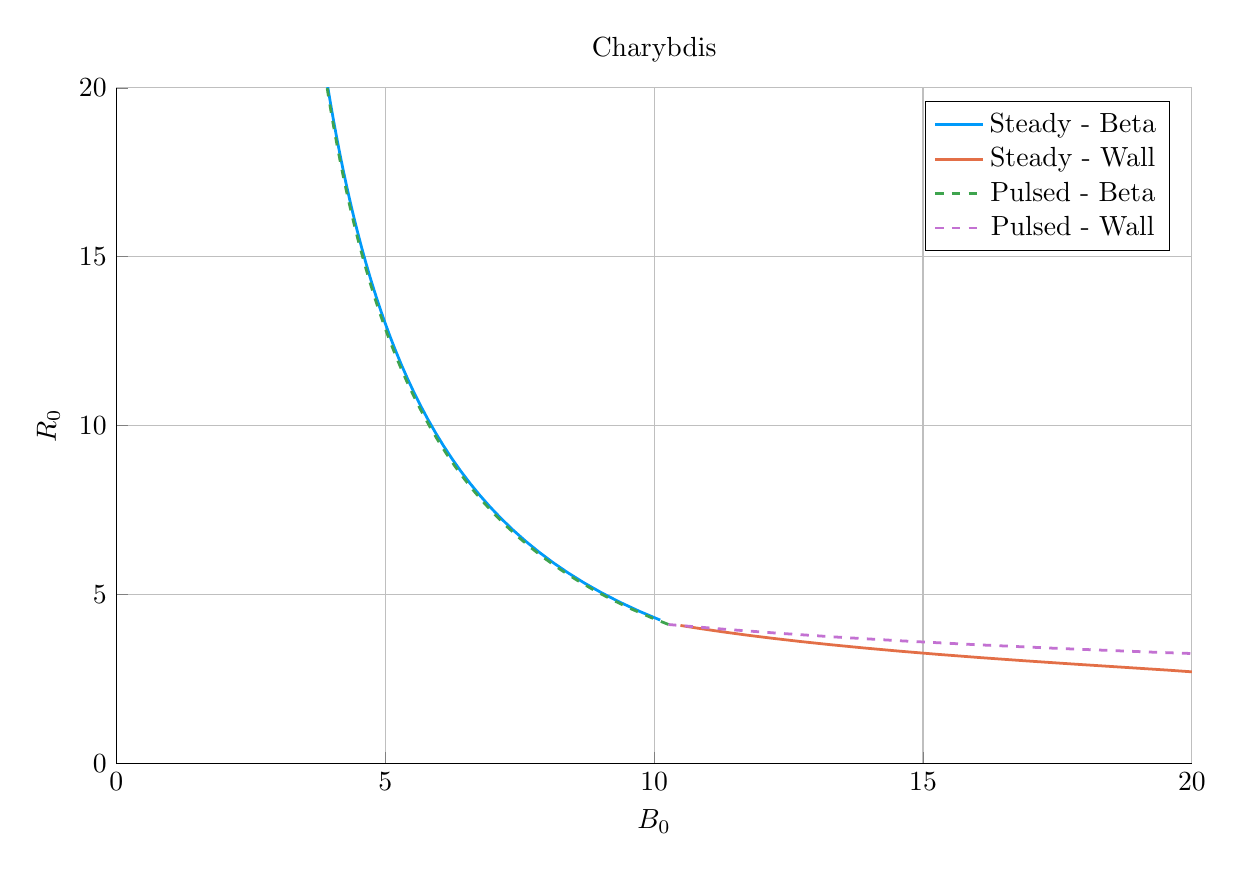
\begin{tikzpicture}[]
\begin{axis}[height = {101.6mm}, ylabel = {${R}_{0}$}, title = {Charybdis}, xmin = {0.0}, xmax = {20.0}, ymax = {20.0}, xlabel = {${B}_{0}$}, {unbounded coords=jump, scaled x ticks = false, xticklabel style={rotate = 0}, xmajorgrids = true, xtick = {0.0,5.0,10.0,15.0,20.0}, xticklabels = {0,5,10,15,20}, xtick align = inside, axis lines* = left, scaled y ticks = false, yticklabel style={rotate = 0}, ymajorgrids = true, ytick = {0.0,5.0,10.0,15.0,20.0}, yticklabels = {0,5,10,15,20}, ytick align = inside, axis lines* = left,     xshift = 0.0mm,
    yshift = 0.0mm,
    axis background/.style={fill={rgb,1:red,1.00000000;green,1.00000000;blue,1.00000000}}
, colorbar style={title=}}, ymin = {0.0}, width = {152.4mm}]\addplot+ [color = {rgb,1:red,0.00000000;green,0.60560316;blue,0.97868012},
draw opacity=1.0,
line width=1,
solid,mark = none,
mark size = 2.0,
mark options = {
    color = {rgb,1:red,0.00000000;green,0.00000000;blue,0.00000000}, draw opacity = 1.0,
    fill = {rgb,1:red,0.00000000;green,0.60560316;blue,0.97868012}, fill opacity = 1.0,
    line width = 1,
    rotate = 0,
    solid
}]coordinates {
(10.112818033153026, 4.241771689478311)
(9.722156888543116, 4.504138117525138)
(9.357875603858393, 4.77497367032698)
(9.017653755630063, 5.054228410858618)
(8.6995124437054, 5.34178832481448)
(8.401566530516865, 5.637594610921002)
(8.122163706328223, 5.941556970897918)
(7.859819415455661, 6.2535750482800845)
(7.613196557650265, 6.5735387749268055)
(7.381088038653343, 6.901328733442317)
(7.162401716104116, 7.236816533350192)
(6.956147367527331, 7.579865198961832)
(6.761425371986388, 7.930329566972662)
(6.577416849463348, 8.28805669191591)
(6.403375044688587, 8.652886257700402)
(6.2386177769852695, 9.02465099355178)
(6.0825208065966905, 9.403177092267818)
(5.934511989185341, 9.788284632344096)
(5.794066116682695, 10.179787994954152)
(5.660700347012839, 10.577496284633074)
(5.533970150598111, 10.981213744847159)
(5.413465705416883, 11.390740170754555)
(5.298808685607224, 11.805871315185586)
(5.189649392059402, 12.226399293085946)
(5.085664187259174, 12.652112975136994)
(4.986553195072601, 13.082798376170517)
(4.892038235455667, 13.518239035062717)
(4.801860966679364, 13.958216385902286)
(4.7157812114040425, 14.402510119861804)
(4.633575445956479, 14.850898537267405)
(4.5550354347559185, 15.303158889428241)
(4.479966994069385, 15.759067709846747)
(4.408188871204256, 16.21840113449116)
(4.33953172691477, 16.680935210866018)
(4.273837210246432, 17.14644619566822)
(4.210957116299974, 17.614710840865197)
(4.15075261849161, 18.085506668079862)
(4.0930935678432965, 18.558612231207235)
(4.037857852672517, 19.03380736722975)
(3.9849308127842145, 19.510873435234036)
(3.9342047029103653, 19.98959354366903)
(3.8855782007091695, 20.46975276591405)
(3.838955955133626, 20.951138344257103)
(3.7942481714200484, 21.433539882408354)
(3.7513702293348077, 21.91674952670236)
(3.710242331663442, 22.400562136158193)
(3.6707891802306123, 22.88477544159215)
(3.6329396770109583, 23.369190193993973)
(3.5966266481325166, 23.853610302391182)
(3.5617865887889004, 24.33784296144382)
(3.5283594272686503, 24.821698769019683)
(3.496288306480746, 25.30499183401733)
(3.465519381509793, 25.787539874702443)
(3.4360016318699595, 26.2691643078435)
(3.4076866872513096, 26.74969032892794)
(3.380528665662031, 27.228946983749)
(3.3544840229690007, 27.706767231660894)
(3.3295114129297314, 28.18298800079238)
(3.3055715568879336, 28.6574502355218)
(3.2826271223788512, 29.129998936506894)
(3.260642607548369, 29.600483215419466)
(3.239584247604666, 30.068756211731234)
(3.2194198921826622, 30.53467533068977)
(3.2001189373344725, 30.998102038032528)
(3.181652227422265, 31.45890197647381)
(3.163991977015565, 31.916944945395528)
(3.1471116955378684, 32.37210489697581)
(3.130986116696265, 32.82425992717794)
(3.115591132350856, 33.27329226186858)
(3.1009037305081053, 33.719088238329654)
(3.0869019371473265, 34.16153828242195)
(3.0735647616124355, 34.600536881650775)
(3.0608721453218655, 35.035982554380354)
};
\addlegendentry{Steady - Beta}
\addplot+ [color = {rgb,1:red,0.88887350;green,0.43564919;blue,0.27812294},
draw opacity=1.0,
line width=1,
solid,mark = none,
mark size = 2.0,
mark options = {
    color = {rgb,1:red,0.00000000;green,0.00000000;blue,0.00000000}, draw opacity = 1.0,
    fill = {rgb,1:red,0.88887350;green,0.43564919;blue,0.27812294}, fill opacity = 1.0,
    line width = 1,
    rotate = 0,
    solid
}]coordinates {
(20.758867641064707, 2.5885674971573294)
(20.346250098246923, 2.6701608818805265)
(19.57104597888471, 2.7580768645580767)
(18.681781921115476, 2.84914579801761)
(17.775790175980152, 2.942053074257325)
(16.896654716492492, 3.036102404206255)
(16.063927450323227, 3.1308756359103893)
(15.285557510665852, 3.226095678435203)
(14.563500533069154, 3.3215674678202314)
(13.896568848875791, 3.417147967307318)
(13.281970890030232, 3.5127292434426214)
(12.716170469467318, 3.6082281475654683)
(12.195372283741088, 3.7035796419955296)
(11.715794270833433, 3.798732281084355)
(11.273815669498969, 3.8936450383948094)
(10.866051794088186, 3.9882850129983627)
(10.489365023931143, 4.08262666943062)
};
\addlegendentry{Steady - Wall}
\addplot+ [color = {rgb,1:red,0.24222430;green,0.64327509;blue,0.30444865},
draw opacity=1.0,
line width=1,
dashed,mark = none,
mark size = 2.0,
mark options = {
    color = {rgb,1:red,0.00000000;green,0.00000000;blue,0.00000000}, draw opacity = 1.0,
    fill = {rgb,1:red,0.24222430;green,0.64327509;blue,0.30444865}, fill opacity = 1.0,
    line width = 1,
    rotate = 0,
    solid
}]coordinates {
(10.26788634689966, 4.1112515557786775)
(9.953967652326213, 4.3094639978912825)
(9.567926244368271, 4.576742787082168)
(9.207974394987358, 4.852707848855866)
(8.871841888699304, 5.137296446755483)
(8.557505525932248, 5.430432251844937)
(8.263156925406376, 5.732025498645217)
(7.9871752024348766, 6.041973183885721)
(7.728103682045175, 6.3601593098028015)
(7.484629973620137, 6.686455168691173)
(7.255568856523303, 7.020719666856628)
(7.039847526735421, 7.362799685753208)
(6.836492834698909, 7.712530477959993)
(6.644620209081183, 8.06973609553486)
(6.463424013335149, 8.43422984818008)
(6.2921691243175495, 8.80581478856818)
(6.13018355681404, 9.184284222105854)
(5.97685198655569, 9.569422237740964)
(5.831610044919842, 9.961004260702955)
(5.693939286027163, 10.358797615092055)
(5.563362729090489, 10.762562105803609)
(5.439440906144732, 11.172050607751359)
(5.321768347746793, 11.587009663771289)
(5.209970453003084, 12.007180084871303)
(5.103700692769835, 12.43229755779498)
(5.002638109938164, 12.862093246958203)
(4.906485077678376, 13.296294396161224)
(4.814965286571576, 13.734624924501638)
(4.727821933804548, 14.176806014771396)
(4.644816091323922, 14.622556692215932)
(4.565725232806084, 15.071594391671503)
(4.490341901840154, 15.523635511246878)
(4.418472505906755, 15.978395950871612)
(4.349936222622964, 16.435591634187325)
(4.284564006352339, 16.89493901242702)
(4.222197684694192, 17.3561555490841)
(4.162689135592264, 17.818960184341037)
(4.105899536872315, 18.283073778386605)
(4.051698680949713, 18.748219532911282)
(3.9999643482627323, 19.214123390225897)
(3.9505817337017928, 19.680514409594025)
(3.903442920928527, 20.147125120523665)
(3.858446400032002, 20.613691852887264)
(3.8154966244515616, 21.079955043879853)
(3.7745036035252744, 21.545659521938795)
(3.7353825273991994, 22.010554767868463)
(3.6980534213689746, 22.47439515350876)
(3.6624408270205375, 22.936940158387063)
(3.62847350780097, 23.397954564874027)
(3.5960841768845415, 23.85720863243935)
(3.565209245407392, 24.314478251672824)
(3.5357885893311605, 24.769545078785413)
(3.5077653333614305, 25.22219665136009)
(3.4810856504959875, 25.672226486155235)
(3.4556985759109375, 26.119434159797105)
(3.4315558340122845, 26.563625373217942)
(3.408611677587535, 27.004612000714285)
(3.3868227380888998, 27.44221212450356)
(3.36614788616562, 27.876250055664674)
(3.3465481016421226, 28.306556342336567)
(3.327986352208224, 28.732967766047434)
(3.3104274769652595, 29.155327355093103)
(3.2938380965241474, 29.573484219331384)
(3.278186482171801, 29.987293796610192)
(3.263442495132517, 30.396617529277517)
(3.2495774839156075, 30.801322953869263)
(3.236564206241785, 31.2012836153002)
(3.224376752844934, 31.596379002720997)
(3.212990475972638, 31.98649447963656)
(3.2023819222517877, 32.371521208907616)
(3.192528769611062, 32.751356073231776)
(3.1834097679780142, 33.12590159165121)
(3.1750046834890777, 33.49506583261046)
(3.1672942459724482, 33.8587623240416)
};
\addlegendentry{Pulsed - Beta}
\addplot+ [color = {rgb,1:red,0.76444018;green,0.44411178;blue,0.82429754},
draw opacity=1.0,
line width=1,
dashed,mark = none,
mark size = 2.0,
mark options = {
    color = {rgb,1:red,0.00000000;green,0.00000000;blue,0.00000000}, draw opacity = 1.0,
    fill = {rgb,1:red,0.76444018;green,0.44411178;blue,0.82429754}, fill opacity = 1.0,
    line width = 1,
    rotate = 0,
    solid
}]coordinates {
(48.990476413653056, 2.408463256282958)
(42.83950920694117, 2.5157944044289065)
(37.687790427214495, 2.623911121514849)
(33.33937742845888, 2.732773154793489)
(29.64296398154308, 2.8423415573543895)
(26.48039367255613, 2.9525785265823425)
(23.758442882319894, 3.0634472709719978)
(21.402860298405816, 3.174911900538905)
(19.353987387634486, 3.2869373368800954)
(17.563502020363714, 3.3994892396762393)
(15.991970371213752, 3.512533946790301)
(14.606987499719377, 3.6260384258753686)
(13.381751501116137, 3.7399702354868722)
(12.293960329570087, 3.854297494171075)
(11.32495111804522, 3.9689888562032056)
(10.459023415380802, 4.084013492866982)
(10.26788634689966, 4.1112515557786775)
};
\addlegendentry{Pulsed - Wall}
\end{axis}

\end{tikzpicture}

    \end{adjustbox}
        \caption{Charybdis Reactor}
    \end{subfigure}
    \hfill
    \begin{subfigure}[t]{0.45\textwidth}
        \centering
    \begin{adjustbox}{width=\textwidth}
      \Large
      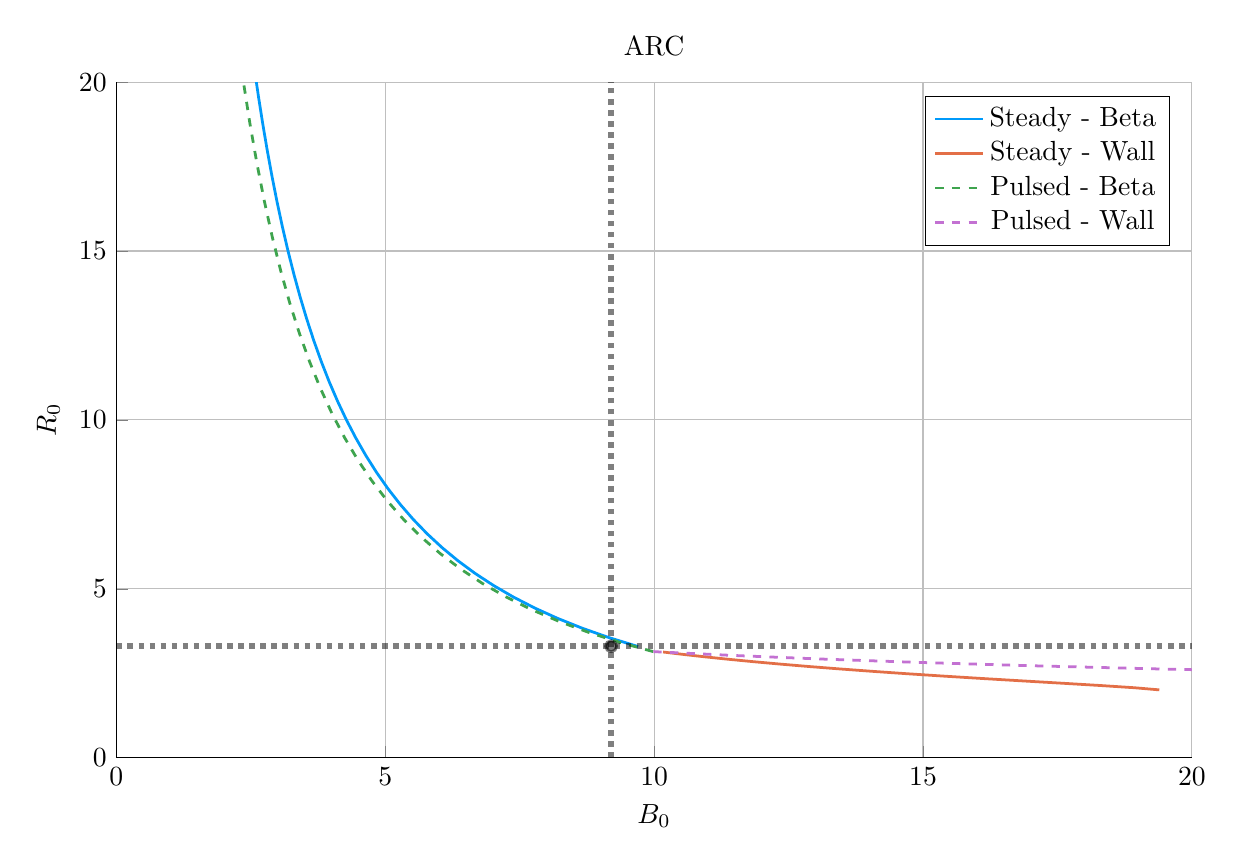
\begin{tikzpicture}[]
\begin{axis}[height = {101.6mm}, ylabel = {${R}_{0}$}, title = {ARC}, xmin = {0.0}, xmax = {20.0}, ymax = {20.0}, xlabel = {${B}_{0}$}, {unbounded coords=jump, scaled x ticks = false, xticklabel style={rotate = 0}, xmajorgrids = true, xtick = {0.0,5.0,10.0,15.0,20.0}, xticklabels = {0,5,10,15,20}, xtick align = inside, axis lines* = left, scaled y ticks = false, yticklabel style={rotate = 0}, ymajorgrids = true, ytick = {0.0,5.0,10.0,15.0,20.0}, yticklabels = {0,5,10,15,20}, ytick align = inside, axis lines* = left,     xshift = 0.0mm,
    yshift = 0.0mm,
    axis background/.style={fill={rgb,1:red,1.00000000;green,1.00000000;blue,1.00000000}}
, colorbar style={title=}}, ymin = {0.0}, width = {152.4mm}]\addplot+ [color = {rgb,1:red,0.00000000;green,0.60560316;blue,0.97868012},
draw opacity=1.0,
line width=1,
solid,mark = none,
mark size = 2.0,
mark options = {
    color = {rgb,1:red,0.00000000;green,0.00000000;blue,0.00000000}, draw opacity = 1.0,
    fill = {rgb,1:red,0.00000000;green,0.60560316;blue,0.97868012}, fill opacity = 1.0,
    line width = 1,
    rotate = 0,
    solid
}]coordinates {
(9.701206080853105, 3.2904233285656006)
(9.162315904693079, 3.553631706046861)
(8.664301107137337, 3.8315748016260343)
(8.203576462497304, 4.124583886864978)
(7.776718537485166, 4.433072975674755)
(7.380720231870917, 4.75741949036414)
(7.012886014999712, 5.097987291342331)
(6.670795005901889, 5.4551257000070565)
(6.352268997292712, 5.829168567645448)
(6.055344682097163, 6.220433393277178)
(5.778249464564785, 6.629220493040615)
(5.519380338856715, 7.05581222339423)
(5.2772854007125325, 7.500472260074458)
(5.050647625972996, 7.963444934423652)
(4.838270606140816, 8.444954628380609)
(4.639065978019038, 8.94520522910952)
(4.4520423235376105, 9.464379643936518)
(4.276295348572609, 10.002639375969222)
(4.110999177018484, 10.56012416048812)
(3.9553986195015125, 11.136951661929974)
(3.8088022956698633, 11.733217231026282)
(3.6705765055641186, 12.34899372141899)
(3.54013975965751, 12.984331364849716)
(3.4169578891619192, 13.639257703809928)
(3.30053966845824, 14.313777580345645)
(3.1904328903033052, 15.007873179535935)
(3.086220842019516, 15.721504126002731)
(2.9875191373772063, 16.45460763166718)
(2.8939728644914635, 17.207098692842226)
(2.8052540149097247, 17.97887033463821)
(2.7210591632720242, 18.7697939005645)
(2.6411073705789065, 19.579719385129263)
(2.565138287279709, 20.40847580717446)
(2.492910435164382, 21.255871621630877)
(2.4241996494611984, 22.12169516733927)
(2.3587976646588236, 23.0057151485579)
(2.296510829425685, 23.907681147764652)
(2.237158937627476, 24.827324167354146)
(2.180574163874242, 25.764357197843207)
(2.126600093288366, 26.71847581021091)
(2.075090836295778, 27.689358770027713)
(2.0259102202234582, 28.676668671060817)
(1.978931050353818, 29.68005258608471)
(1.9340344338545452, 30.69914273267572)
(1.8911091606836798, 31.733557151818793)
(1.8500511361739687, 32.78290039722107)
(1.8107628605384507, 33.846764233283025)
(1.773152951016952, 34.92472833975579)
(1.7371357028100902, 36.01636102117257)
(1.7026306853269466, 37.121219919229354)
(1.6695623706125668, 38.23885272635799)
(1.6378597911249178, 39.368797898817405)
(1.607456224302725, 40.51058536770822)
(1.5782889016090462, 41.663737246396295)
(1.5502987399539199, 42.82776853291479)
(1.5234300935954943, 44.00218780599217)
(1.4976305247952577, 45.18649791343829)
(1.4728505916614916, 46.38019665170201)
(1.4490436517578602, 47.58277743549339)
(1.4261656801829077, 48.79372995643627)
};
\addlegendentry{Steady - Beta}
\addplot+ [color = {rgb,1:red,0.88887350;green,0.43564919;blue,0.27812294},
draw opacity=1.0,
line width=1,
solid,mark = none,
mark size = 2.0,
mark options = {
    color = {rgb,1:red,0.00000000;green,0.00000000;blue,0.00000000}, draw opacity = 1.0,
    fill = {rgb,1:red,0.88887350;green,0.43564919;blue,0.27812294}, fill opacity = 1.0,
    line width = 1,
    rotate = 0,
    solid
}]coordinates {
(19.394007482712425, 2.006855814841082)
(18.932196567189358, 2.070220226465634)
(18.296989378345195, 2.1362327099649083)
(17.587029315408756, 2.2039322514902886)
(16.847882407994106, 2.272885741349308)
(16.111374502564406, 2.3427307443133163)
(15.396027314547156, 2.4132115621474344)
(14.710952688793137, 2.484165095168367)
(14.06168447794857, 2.555449485048069)
(13.450465418483889, 2.6269568263788754)
(12.877644538645335, 2.6986005527245354)
(12.342394470642008, 2.7703103261458715)
(11.843182246608265, 2.8420284550528074)
(11.376441269625893, 2.9137564749008216)
(10.944966372727551, 2.985307257194073)
(10.541663878705513, 3.056795384934831)
(10.165908182236457, 3.128148092221394)
};
\addlegendentry{Steady - Wall}
\addplot+ [color = {rgb,1:red,0.24222430;green,0.64327509;blue,0.30444865},
draw opacity=1.0,
line width=1,
dashed,mark = none,
mark size = 2.0,
mark options = {
    color = {rgb,1:red,0.00000000;green,0.00000000;blue,0.00000000}, draw opacity = 1.0,
    fill = {rgb,1:red,0.24222430;green,0.64327509;blue,0.30444865}, fill opacity = 1.0,
    line width = 1,
    rotate = 0,
    solid
}]coordinates {
(9.980483622051658, 3.1402982942956537)
(9.392786903460065, 3.3984668375583613)
(8.79273598103983, 3.7029994270206985)
(8.23820290909994, 4.029752381934837)
(7.725182218401588, 4.380005330007902)
(7.250078106370205, 4.755088191072525)
(6.80965553466646, 5.15638156809462)
(6.400998063035608, 5.585317075247801)
(6.0214713600430425, 6.043377623224966)
(5.668691517461799, 6.532097691007738)
(5.340497445229901, 7.053063624618788)
(5.034926745580058, 7.607914017422467)
(4.750194564008521, 8.198340243900201)
(4.484674995755211, 8.826087240213646)
(4.236884692979903, 9.49295465115087)
(4.00546837264544, 10.200798495308337)
(3.7891859704718387, 10.951533539957822)
(3.5869012239550364, 11.747136625739826)
(3.3975714987448393, 12.589651241396528)
(3.2202386987489797, 13.481193723261853)
(3.0540211220494466, 14.423961547290066)
(2.8981061427709687, 15.420244298711943)
(2.7517436139566023, 16.472438053930638)
(2.6142398986781377, 17.58306410230943)
(2.4849524463010138, 18.754793188384546)
(2.363284838174807, 19.990476791576892)
(2.248682232019848, 21.293187416028662)
(2.140627136740878, 22.666270490916787)
(2.038635448877246, 24.113411362836906)
(1.9422526775794744, 25.638722123308433)
(1.8510502754751532, 27.246854857488287)
(1.7646219756564088, 28.94315065234289)
(1.6825800061969869, 30.73383791051506)
(1.6045510059627948, 32.62630011975996)
(1.53017138625397, 34.629443897654504)
(1.4590817483192686, 36.754215952550474)
(1.3909197311384796, 39.01434852880224)
(1.3253102336217724, 41.42746903285954)
(1.261851128383913, 44.01681696754988)
(1.20009089049112, 46.81403058684408)
(1.1394908096975784, 49.863950342519615)
};
\addlegendentry{Pulsed - Beta}
\addplot+ [color = {rgb,1:red,0.76444018;green,0.44411178;blue,0.82429754},
draw opacity=1.0,
line width=1,
dashed,mark = none,
mark size = 2.0,
mark options = {
    color = {rgb,1:red,0.00000000;green,0.00000000;blue,0.00000000}, draw opacity = 1.0,
    fill = {rgb,1:red,0.76444018;green,0.44411178;blue,0.82429754}, fill opacity = 1.0,
    line width = 1,
    rotate = 0,
    solid
}]coordinates {
(29.27715761652869, 2.3448804182939873)
(25.4410619834368, 2.4377937236066716)
(22.158819835998365, 2.5322208586485804)
(19.342453256965573, 2.628163744265164)
(16.919364280634177, 2.7256238396687067)
(14.829378672669455, 2.8246020951898183)
(13.022412368922526, 2.9250989082568273)
(11.456617692058645, 3.0271140820266207)
(10.096901921254785, 3.1306467862637533)
(9.980483622051658, 3.1402982942956537)
};
\addlegendentry{Pulsed - Wall}
\addplot+ [color = {rgb,1:red,0.00000000;green,0.00000000;blue,0.00000000},
draw opacity=0.5,
line width=2,
dotted,mark = none,
mark size = 2.0,
mark options = {
    color = {rgb,1:red,0.00000000;green,0.00000000;blue,0.00000000}, draw opacity = 0.5,
    fill = {rgb,1:red,0.00000000;green,0.00000000;blue,0.00000000}, fill opacity = 0.5,
    line width = 1,
    rotate = 0,
    solid
},forget plot]coordinates {
(0.0, 3.3)
(20.0, 3.3)
};
\addplot+ [color = {rgb,1:red,0.00000000;green,0.00000000;blue,0.00000000},
draw opacity=0.5,
line width=2,
dotted,mark = none,
mark size = 2.0,
mark options = {
    color = {rgb,1:red,0.00000000;green,0.00000000;blue,0.00000000}, draw opacity = 0.5,
    fill = {rgb,1:red,0.00000000;green,0.00000000;blue,0.00000000}, fill opacity = 0.5,
    line width = 1,
    rotate = 0,
    solid
},forget plot]coordinates {
(9.2, 0.0)
(9.2, 20.0)
};
\addplot+[draw=none, color = {rgb,1:red,0.00000000;green,0.00000000;blue,0.00000000},
draw opacity=0.5,
line width=0,
solid,mark = *,
mark size = 2.0,
mark options = {
    color = {rgb,1:red,0.00000000;green,0.00000000;blue,0.00000000}, draw opacity = 0.5,
    fill = {rgb,1:red,0.00000000;green,0.00000000;blue,0.00000000}, fill opacity = 0.5,
    line width = 1,
    rotate = 0,
    solid
},forget plot] coordinates {
(9.2, 3.3)
};
\end{axis}

\end{tikzpicture}

    \end{adjustbox}
        \caption{ARC Reactor}
    \end{subfigure}
    \hfill \hfill ~\\ ~\\ ~\\
    \caption{Steady State Prototype Comparison} ~\\
    \label{fig:charybdis}
\end{figure*}

\begin{table}[b!]
\centering
\caption{Charybdis Variables}
\hfill
\begin{subtable}[t]{0.4\textwidth}
\centering
\caption{Input Variables} ~\\
\begin{tabular}{ c|c }

Input            & Value           \\
\hline
$H$              & 1.7              \\
$Q$              & 25.0             \\
$N_{G}$          & 0.9              \\
$\varepsilon$       & 0.3              \\
$\kappa_{95}$    & 1.8              \\
$\delta_{95}$    & 0.35             \\
$\nu_{n}$        & 0.4              \\
$\nu_{T}$        & 1.1              \\
$l_{i}$          & 0.558         \\
$A$              & 2.5              \\
$Z_{eff}$        & 1.75             \\
$f_{D}$          & 0.9              \\
$\tau_{FT}$      & 1.6e9            \\
$B_{CS}$         & 12.0             \\

\end{tabular}
\end{subtable}
\hfill
\begin{subtable}[t]{0.5\textwidth}
\centering
\caption{Output Variables} ~\\
\begin{tabular}{ c|c }

Output           & Value       \\
\hline
$R_{0}$          & 4.13            \\
$B_{0}$          & 10.28            \\
$I_{P}$          & 8.98            \\
$\overline n$    & 1.47            \\
$\overline T$    & 15.81           \\
$\beta_{N}$       & 0.028            \\
$q_{95}$         & 6.089            \\
$P_{W}$          & 3.003            \\
$f_{BS}$         & 0.723           \\
$f_{CD}$         & 0.277           \\
$f_{ID}$         & 0.0              \\
$\volume$         & 225.5            \\
$P_{F}$          & 1294           \\
$\eta_{CD}$      & 0.291           \\

\end{tabular}
\end{subtable}
\hfill
\hfill
\label{table:charybdis}
\end{table}

\begin{figure*}[t!]
    \centering
    \hfill
    \begin{subfigure}[t]{0.45\textwidth}
        \centering
    \begin{adjustbox}{width=\textwidth}
      \Large
      \input{images/comparisons/proteus_R_0_vs_B_0}
    \end{adjustbox}
        \caption{Proteus Reactor}
    \end{subfigure}
    \hfill
    \begin{subfigure}[t]{0.45\textwidth}
        \centering
    \begin{adjustbox}{width=\textwidth}
      \Large
      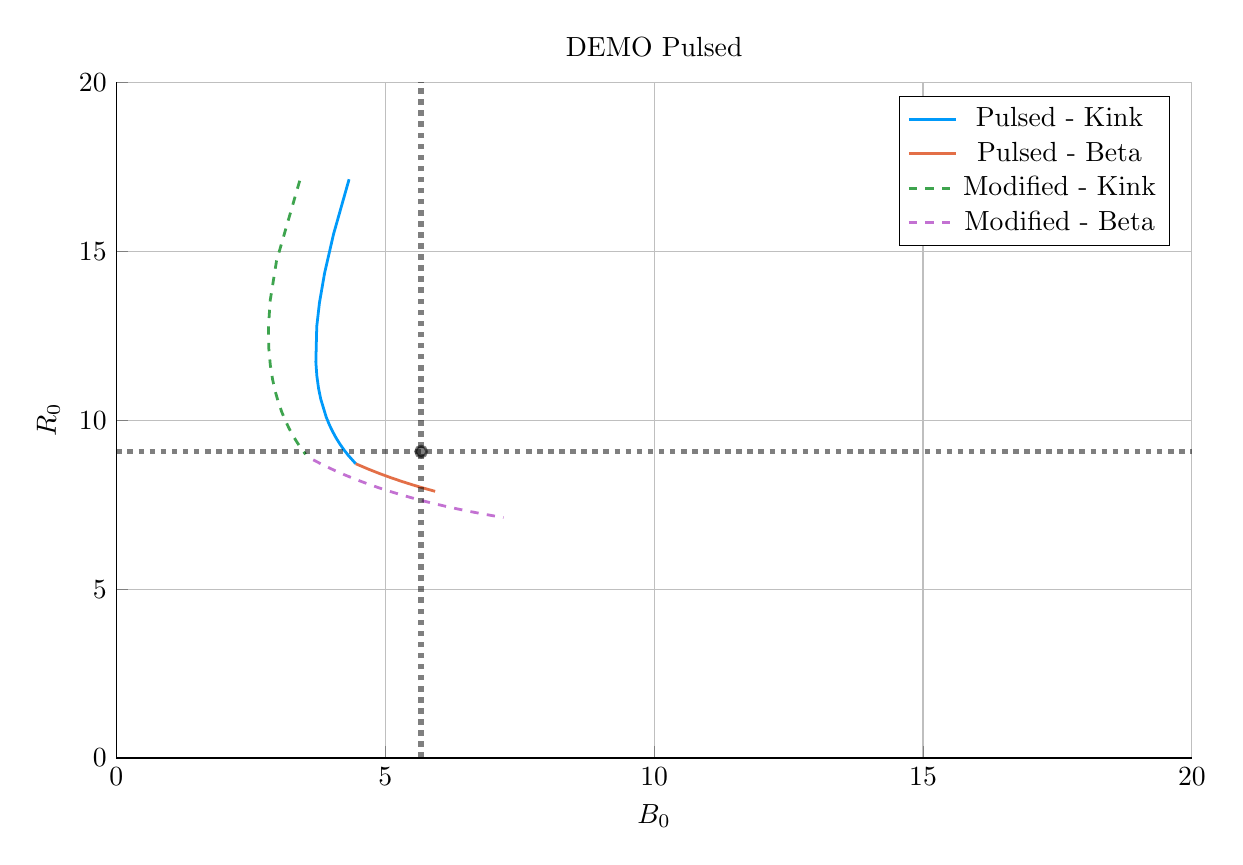
\begin{tikzpicture}[]
\begin{axis}[height = {101.6mm}, ylabel = {${R}_{0}$}, title = {DEMO Pulsed}, xmin = {0.0}, xmax = {20.0}, ymax = {20.0}, xlabel = {${B}_{0}$}, {unbounded coords=jump, scaled x ticks = false, xticklabel style={rotate = 0}, xmajorgrids = true, xtick = {0.0,5.0,10.0,15.0,20.0}, xticklabels = {0,5,10,15,20}, xtick align = inside, axis lines* = left, scaled y ticks = false, yticklabel style={rotate = 0}, ymajorgrids = true, ytick = {0.0,5.0,10.0,15.0,20.0}, yticklabels = {0,5,10,15,20}, ytick align = inside, axis lines* = left,     xshift = 0.0mm,
    yshift = 0.0mm,
    axis background/.style={fill={rgb,1:red,1.00000000;green,1.00000000;blue,1.00000000}}
, colorbar style={title=}}, ymin = {0.0}, width = {152.4mm}]\addplot+ [color = {rgb,1:red,0.00000000;green,0.60560316;blue,0.97868012},
draw opacity=1.0,
line width=1,
solid,mark = none,
mark size = 2.0,
mark options = {
    color = {rgb,1:red,0.00000000;green,0.00000000;blue,0.00000000}, draw opacity = 1.0,
    fill = {rgb,1:red,0.00000000;green,0.60560316;blue,0.97868012}, fill opacity = 1.0,
    line width = 1,
    rotate = 0,
    solid
}]coordinates {
(4.327031075670194, 17.134796748649162)
(4.038214026054326, 15.511755022601415)
(3.8713719163129245, 14.355562963913712)
(3.7758613845615545, 13.476675762289453)
(3.7257856761317214, 12.778294295391971)
(3.7090473695925437, 11.723065749829066)
(3.727711597554826, 11.30970201784727)
(3.7586131667481433, 10.94971275897184)
(3.799052518631718, 10.632190690377048)
(3.901290136389271, 10.09455415135144)
(3.960577465316514, 9.863813619410237)
(4.0241209645210345, 9.653307397969705)
(4.0912717805663785, 9.460162902699798)
(4.161514602943343, 9.28206292757184)
(4.2344343960723005, 9.117114543572253)
(4.309692554546368, 8.963753917462126)
(4.450417240491067, 8.712493965092264)
};
\addlegendentry{Pulsed - Kink}
\addplot+ [color = {rgb,1:red,0.88887350;green,0.43564919;blue,0.27812294},
draw opacity=1.0,
line width=1,
solid,mark = none,
mark size = 2.0,
mark options = {
    color = {rgb,1:red,0.00000000;green,0.00000000;blue,0.00000000}, draw opacity = 1.0,
    fill = {rgb,1:red,0.88887350;green,0.43564919;blue,0.27812294}, fill opacity = 1.0,
    line width = 1,
    rotate = 0,
    solid
}]coordinates {
(4.450417240491067, 8.712493965092264)
(4.490148631384312, 8.684308742646298)
(4.692490181445514, 8.547262773806349)
(4.8960344619053355, 8.41947837460442)
(5.100651132702229, 8.30014929484307)
(5.306202822090688, 8.188581738801314)
(5.512545696627038, 8.084175191078112)
(5.719530043226767, 7.986407002697611)
(5.927000883375481, 7.894819882619234)
};
\addlegendentry{Pulsed - Beta}
\addplot+ [color = {rgb,1:red,0.24222430;green,0.64327509;blue,0.30444865},
draw opacity=1.0,
line width=1,
dashed,mark = none,
mark size = 2.0,
mark options = {
    color = {rgb,1:red,0.00000000;green,0.00000000;blue,0.00000000}, draw opacity = 1.0,
    fill = {rgb,1:red,0.24222430;green,0.64327509;blue,0.30444865}, fill opacity = 1.0,
    line width = 1,
    rotate = 0,
    solid
}]coordinates {
(3.4087424183072135, 17.090884129081292)
(2.977074181068944, 14.713048632784332)
(2.8592500074202523, 13.541171522519205)
(2.827199220063259, 12.740024138753894)
(2.8339789008667826, 12.12574468151967)
(2.862412302880871, 11.626187613249266)
(2.9044598258085443, 11.205091848948229)
(2.95577893007882, 10.841432203317366)
(3.0137895352525907, 10.521822649209419)
(3.076849710218805, 10.23716073884787)
(3.1438583711612704, 9.980947801083442)
(3.214045733980633, 9.748367275345563)
(3.2868548955983727, 9.535742205343247)
(3.361871149981842, 9.340197658526863)
(3.4387778750377818, 9.15944098345979)
(3.5173279629378453, 8.991613349767409)
};
\addlegendentry{Modified - Kink}
\addplot+ [color = {rgb,1:red,0.76444018;green,0.44411178;blue,0.82429754},
draw opacity=1.0,
line width=1,
dashed,mark = none,
mark size = 2.0,
mark options = {
    color = {rgb,1:red,0.00000000;green,0.00000000;blue,0.00000000}, draw opacity = 1.0,
    fill = {rgb,1:red,0.76444018;green,0.44411178;blue,0.82429754}, fill opacity = 1.0,
    line width = 1,
    rotate = 0,
    solid
}]coordinates {
(3.6607028750648505, 8.825949645171955)
(3.8574448036470477, 8.664618827122876)
(4.056375867871351, 8.51434867582932)
(4.257366397480293, 8.374075613831488)
(4.460279103534801, 8.242896218794312)
(4.664969389370631, 8.12003771613466)
(4.871285596007394, 8.004834914067093)
(5.07906923307514, 7.896711937521184)
(5.288155233306219, 7.795167587687744)
(5.498372259673351, 7.699763475973523)
(5.709543087166185, 7.610114306522102)
(5.921485076209294, 7.525879840414137)
(6.134010749367255, 7.446758190646709)
(6.346928478632384, 7.372480180910637)
(6.560043285872518, 7.302804563889649)
(6.773157754368795, 7.237513941672651)
(6.986073044284746, 7.176411266758267)
(7.198590001107076, 7.119316828230052)
};
\addlegendentry{Modified - Beta}
\addplot+ [color = {rgb,1:red,0.00000000;green,0.00000000;blue,0.00000000},
draw opacity=0.5,
line width=2,
dotted,mark = none,
mark size = 2.0,
mark options = {
    color = {rgb,1:red,0.00000000;green,0.00000000;blue,0.00000000}, draw opacity = 0.5,
    fill = {rgb,1:red,0.00000000;green,0.00000000;blue,0.00000000}, fill opacity = 0.5,
    line width = 1,
    rotate = 0,
    solid
},forget plot]coordinates {
(0.0, 9.072)
(20.0, 9.072)
};
\addplot+ [color = {rgb,1:red,0.00000000;green,0.00000000;blue,0.00000000},
draw opacity=0.5,
line width=2,
dotted,mark = none,
mark size = 2.0,
mark options = {
    color = {rgb,1:red,0.00000000;green,0.00000000;blue,0.00000000}, draw opacity = 0.5,
    fill = {rgb,1:red,0.00000000;green,0.00000000;blue,0.00000000}, fill opacity = 0.5,
    line width = 1,
    rotate = 0,
    solid
},forget plot]coordinates {
(5.667, 0.0)
(5.667, 20.0)
};
\addplot+[draw=none, color = {rgb,1:red,0.00000000;green,0.00000000;blue,0.00000000},
draw opacity=0.5,
line width=0,
solid,mark = *,
mark size = 2.0,
mark options = {
    color = {rgb,1:red,0.00000000;green,0.00000000;blue,0.00000000}, draw opacity = 0.5,
    fill = {rgb,1:red,0.00000000;green,0.00000000;blue,0.00000000}, fill opacity = 0.5,
    line width = 1,
    rotate = 0,
    solid
},forget plot] coordinates {
(5.667, 9.072)
};
\end{axis}

\end{tikzpicture}

    \end{adjustbox}
        \caption{DEMO Pulsed Reactor}
    \end{subfigure}
    \hfill \hfill ~\\ ~\\ ~\\
    \caption{Pulsed Prototype Comparison} ~\\
    \label{fig:proteus}
\end{figure*}

\begin{table}[b!]
\centering
\caption{Proteus Variables}
\hfill
\begin{subtable}[t]{0.4\textwidth}
\centering
\caption{Input Variables} ~\\
\begin{tabular}{ c|c }

Input            & Value           \\
\hline
$H$              & 1.0              \\
$Q$              & 25.0             \\
$N_{G}$          & 0.9              \\
$\varepsilon$       & 0.3              \\
$\kappa_{95}$    & 1.8              \\
$\delta_{95}$    & 0.35             \\
$\nu_{n}$        & 0.4              \\
$\nu_{T}$        & 1.1              \\
$l_{i}$          & 0.633         \\
$A$              & 2.5              \\
$Z_{eff}$        & 1.75             \\
$f_{D}$          & 0.9              \\
$\tau_{FT}$      & 7200           \\
$B_{CS}$         & 20.0             \\

\end{tabular}
\end{subtable}
\hfill
\begin{subtable}[t]{0.5\textwidth}
\centering
\caption{Output Variables} ~\\
\begin{tabular}{ c|c }

Output           & Value       \\
\hline
$R_{0}$          & 6.11             \\
$B_{0}$          & 4.93            \\
$I_{P}$          & 15.54            \\
$\overline n$    & 1.16            \\
$\overline T$    & 11.25            \\
$\beta_{N}$       & 0.028            \\
$q_{95}$         & 2.5              \\
$P_{W}$          & 1.763            \\
$f_{BS}$         & 0.2675           \\
$f_{CD}$         & 0.0              \\
$f_{ID}$         & 0.7325           \\
$\volume$         & 732.6            \\
$P_{F}$          & 1667           \\
$\eta_{CD}$      & 0.0              \\

\end{tabular}
\end{subtable}
\hfill
\hfill
\label{table:proteus}
\end{table}

\clearpage

\newpage

\subsection{Navigating around Charybdis}

The Charybdis reactor is the steady-state twin developed for this paper. As mentioned, its parameters are similar to the ARC design. This is shown in \cref{fig:charybdis}, where the two $R_0$ -- $B_0$ curves are almost interchangeable. Before moving on, it proves useful to note that the optimum place to build on these curves is where the two portions intersect -- as it minimizes costs. \added{These cost curves are shown in \cref{fig:steady_cost}.}

\subsection{Pinning down Proteus}

The pulsed twin reactor, Proteus, highlights the effects of a high field central solenoid. When compared to the Pulsed DEMO design, the $R_0$ -- $B_0$ curve looks far more favorable -- i.e.\ each machine built at a certain magnet strength would be more compact (and cheaper). An interesting facet of Proteus is that it exhibits all three used limits: kink safety factor, Troyon beta, and wall loading. \added{Cost curves are shown in \cref{fig:pulsed_costs}.}

\begin{table}[b!]
\centering
\caption{Proteus and Charybdis Comparison} ~ \\
\small{ The twin pulsed and steady-state prototypes show general trends in terms of what value values the dynamic variables will have. As can be seen, the radius ($R_0$) of the pulsed prototype (Proteus) is two meters larger than its steady-state twin (Charybdis). }
\hfill
\begin{subtable}[t]{0.45\textwidth}
\centering
\caption{Charybdis} ~\\
\begin{tabular}{ c|c }

Output           & Value       \\
\hline
$R_{0}$          & 4.13            \\
$B_{0}$          & 10.28            \\
$I_{P}$          & 8.98            \\
$\overline n$    & 1.47            \\
$\overline T$    & 15.81           \\
$f_{BS}$ & 0.72 \\
$f_{CD}$ & 0.28 \\
$P_F$ & 1300 \\
$W_M$ & 9.48 \\
$C_W$ & 0.007 \\
\end{tabular}
\end{subtable}
\hfill
\begin{subtable}[t]{0.45\textwidth}
\centering
\caption{Proteus} ~\\
\begin{tabular}{ c|c }

Output           & Value       \\
\hline
$R_{0}$          & 6.11             \\
$B_{0}$          & 4.93            \\
$I_{P}$          & 15.54            \\
$\overline n$    & 1.16            \\
$\overline T$    & 11.25            \\
$f_{BS}$ & 0.27 \\
$f_{ID}$ & 0.73 \\
$P_F$ & 1650 \\
$W_M$ & 7.09 \\
$C_W$ & 0.004 \\
\end{tabular}
\end{subtable}
\hfill
\hfill
\label{table:proteus_charybdis} ~ \\ ~ \\ ~ \\  ~ \\
\end{table}

\newpage

\subsection{Highlighting Operation Differences}

\label{subsection:operation_differences}

\added{Before moving onto general conclusions taken from the data, a quick investigation into the pulsed vs steady-state twin results is in order. A comparison between the two is best abridged in \cref{table:proteus_charybdis}.}

\added{Most apparently, pulsed reactors are typically larger than steady-state ones and are meant to be run at higher plasma currents. The former behavior was seen with the DEMO designs,\cite{process,inputfile} -- as the larger size was needed for long pulse lengths.\cite{giruzzi} The latter was then already mentioned in discussing how steady-state reactors never saw a kink (current limiting) regime. Additionally pulsed machines can be run at much lower temperatures because their higher current improves confinement. }

\added{These combined effects lead to the minimum cost reactors for steady-state operation having much higher toroidal field strengths than their pulsed counterparts. This is discussed in \cref{subsection:high_field} when explaining optimum use of HTS tape. }
\section{Learning from the Data}

Now that the model has been properly vetted and prototypes designed, we can explore how pulsed and steady-state tokamaks scale. \replaced{This will lead to}{Fitting with the Dickens theme, there will be} three mostly independent results. The first result will explore how to minimize costs for a reactor by choosing optimum design points. The next will be an argument for how to properly utilize the HTS magnet technology in component design. Lastly, we will take a cursory look at the other parameters capable of lowering machine costs.

\subsection{Picking a Design Point}

\label{subsection:design_point}

With more than twenty design parameters, finding the most \replaced{economic}{efficient} reactor is \replaced{computationally intractable.}{a fool's errand.} Intuition building aside, finding \replaced{optimum}{good} reactors becomes much more feasible when only focusing on \replaced{dynamic}{floating} variables -- i.e.\ when keeping \replaced{static}{fixed} variables constant. This method, for example, is how all the $R_0$ -- $B_0$ curves have been produced this chapter. Once these curves are produced, it is up to the user to choose which reactor on them to build. However, the guiding metric usually involves lowering some cost, either: capital cost or cost-per-watt.

Regardless of reactor type, most \replaced{economic}{efficient} tokamaks operate near the beta limit -- where plasma pressure is greatest. Besides being a regime highly sensitive to magnetic field strength, the beta limit is a constraint that occurs on every reactor (seen by the authors). This beta limit \added{($\beta_N$)} is usually nested between the kink limit \added{($q_*$)} to lower $B_0$ values and wall loading \added{($P_W$)} to higher ones. Understanding these regimes is the first step towards building an intuition favoring \replaced{economic}{efficient} machines -- see \cref{fig:limit_regimes}.

\begin{figure}
\centering
\begin{adjustbox}{width=0.8\textwidth}
	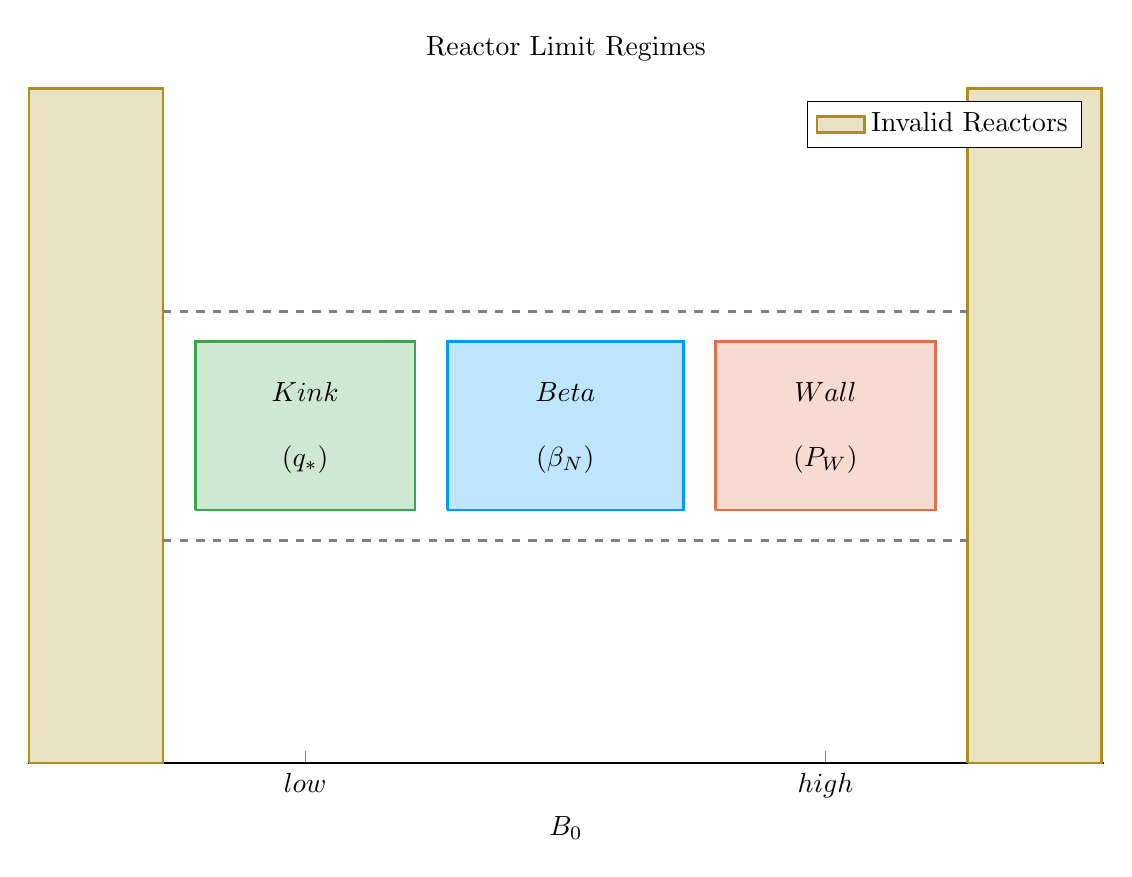
\begin{tikzpicture}[]
\begin{axis}[height = {101.6mm}, ylabel = {}, title = {Reactor Limit Regimes}, xmin = {-0.005}, xmax = {8.015}, ymax = {1.0015}, xlabel = {$B_0$}, {unbounded coords=jump, scaled x ticks = false, xticklabel style={rotate = 0}, xmajorgrids = false, xtick = {2.06,5.94}, xticklabels = {$low$,$high$}, xtick align = inside, axis lines* = left, scaled y ticks = false, yticklabel style={rotate = 0}, ymajorticks=false, ymajorgrids = false, axis lines* = left,     xshift = 0.0mm,
    yshift = 0.0mm,
    axis background/.style={fill={rgb,1:red,1.00000000;green,1.00000000;blue,1.00000000}}
, colorbar style={title=}}, ymin = {0}, width = {152.4mm}]\addplot+ [color = {rgb,1:red,0.67554396;green,0.55566233;blue,0.09423434},
draw opacity=1.0,
line width=1,
solid,mark = none,
mark size = 2.0,
mark options = {
    color = {rgb,1:red,0.00000000;green,0.00000000;blue,0.00000000}, draw opacity = 1.0,
    fill = {rgb,1:red,0.67554396;green,0.55566233;blue,0.09423434}, fill opacity = 1.0,
    line width = 1,
    rotate = 0,
    solid
},fill = {rgb,1:red,0.67554396;green,0.55566233;blue,0.09423434}, fill opacity=0.25,area legend]coordinates {
(0, 0)
(1, 0)
(1, 1)
(0, 1)
(0, 0)
};
\addlegendentry{Invalid Reactors}
\addplot+ [color = {rgb,1:red,0.67554396;green,0.55566233;blue,0.09423434},
draw opacity=1.0,
line width=1,
solid,mark = none,
mark size = 2.0,
mark options = {
    color = {rgb,1:red,0.00000000;green,0.00000000;blue,0.00000000}, draw opacity = 1.0,
    fill = {rgb,1:red,0.67554396;green,0.55566233;blue,0.09423434}, fill opacity = 1.0,
    line width = 1,
    rotate = 0,
    solid
},fill = {rgb,1:red,0.67554396;green,0.55566233;blue,0.09423434}, fill opacity=0.25,forget plot]coordinates {
(7, 0)
(8, 0)
(8, 1)
(7, 1)
(7, 0)
};
\addplot+ [color = {rgb,1:red,0.24222430;green,0.64327509;blue,0.30444865},
draw opacity=1.0,
line width=1,
solid,mark = none,
mark size = 2.0,
mark options = {
    color = {rgb,1:red,0.00000000;green,0.00000000;blue,0.00000000}, draw opacity = 1.0,
    fill = {rgb,1:red,0.24222430;green,0.64327509;blue,0.30444865}, fill opacity = 1.0,
    line width = 1,
    rotate = 0,
    solid
},fill = {rgb,1:red,0.24222430;green,0.64327509;blue,0.30444865}, fill opacity=0.25,forget plot]coordinates {
(1.24, 0.375)
(2.88, 0.375)
(2.88, 0.625)
(1.24, 0.625)
(1.24, 0.375)
};
\addplot+ [color = {rgb,1:red,0.00000000;green,0.60560316;blue,0.97868012},
draw opacity=1.0,
line width=1,
solid,mark = none,
mark size = 2.0,
mark options = {
    color = {rgb,1:red,0.00000000;green,0.00000000;blue,0.00000000}, draw opacity = 1.0,
    fill = {rgb,1:red,0.00000000;green,0.60560316;blue,0.97868012}, fill opacity = 1.0,
    line width = 1,
    rotate = 0,
    solid
},fill = {rgb,1:red,0.00000000;green,0.60560316;blue,0.97868012}, fill opacity=0.25,forget plot]coordinates {
(3.12, 0.375)
(4.88, 0.375)
(4.88, 0.625)
(3.12, 0.625)
(3.12, 0.375)
};
\addplot+ [color = {rgb,1:red,0.88887350;green,0.43564919;blue,0.27812294},
draw opacity=1.0,
line width=1,
solid,mark = none,
mark size = 2.0,
mark options = {
    color = {rgb,1:red,0.00000000;green,0.00000000;blue,0.00000000}, draw opacity = 1.0,
    fill = {rgb,1:red,0.88887350;green,0.43564919;blue,0.27812294}, fill opacity = 1.0,
    line width = 1,
    rotate = 0,
    solid
},fill = {rgb,1:red,0.88887350;green,0.43564919;blue,0.27812294}, fill opacity=0.25,forget plot]coordinates {
(5.12, 0.375)
(6.76, 0.375)
(6.76, 0.625)
(5.12, 0.625)
(5.12, 0.375)
};
\addplot+ [color = {rgb,1:red,0.50196078;green,0.50196078;blue,0.50196078},
draw opacity=1.0,
line width=1,
dashed,mark = none,
mark size = 2.0,
mark options = {
    color = {rgb,1:red,0.00000000;green,0.00000000;blue,0.00000000}, draw opacity = 1.0,
    fill = {rgb,1:red,0.50196078;green,0.50196078;blue,0.50196078}, fill opacity = 1.0,
    line width = 1,
    rotate = 0,
    solid
},forget plot]coordinates {
(1.0, 0.67)
(7.0, 0.67)
};
\addplot+ [color = {rgb,1:red,0.50196078;green,0.50196078;blue,0.50196078},
draw opacity=1.0,
line width=1,
dashed,mark = none,
mark size = 2.0,
mark options = {
    color = {rgb,1:red,0.00000000;green,0.00000000;blue,0.00000000}, draw opacity = 1.0,
    fill = {rgb,1:red,0.50196078;green,0.50196078;blue,0.50196078}, fill opacity = 1.0,
    line width = 1,
    rotate = 0,
    solid
},forget plot]coordinates {
(1.0, 0.32999999999999996)
(7.0, 0.32999999999999996)
};
\node at (axis cs:2.06, 0.55) [,
color={rgb,1:red,0.00000000;green,0.00000000;blue,0.00000000}, draw opacity=1.0,
rotate=0.0
] {$Kink$};
\node at (axis cs:4, 0.55) [,
color={rgb,1:red,0.00000000;green,0.00000000;blue,0.00000000}, draw opacity=1.0,
rotate=0.0
] {$Beta$};
\node at (axis cs:5.94, 0.55) [,
color={rgb,1:red,0.00000000;green,0.00000000;blue,0.00000000}, draw opacity=1.0,
rotate=0.0
] {$Wall$};
\node at (axis cs:2.06, 0.45) [,
color={rgb,1:red,0.00000000;green,0.00000000;blue,0.00000000}, draw opacity=1.0,
rotate=0.0
] {$(q_{*})$};
\node at (axis cs:4, 0.45) [,
color={rgb,1:red,0.00000000;green,0.00000000;blue,0.00000000}, draw opacity=1.0,
rotate=0.0
] {$(\beta_N)$};
\node at (axis cs:5.94, 0.45) [,
color={rgb,1:red,0.00000000;green,0.00000000;blue,0.00000000}, draw opacity=1.0,
rotate=0.0
] {$(P_W)$};
\end{axis}

\end{tikzpicture}

\end{adjustbox}
\caption{\replaced{Limiting Constraint Regimes}{Limit Regimes as function of $B_0$}} ~ \\
\added{\small At a simple level, a reactor has around three regimes of design limiting constraints. At low fields, the kink safety factor -- through $q_*$ and \cref{eq:r_kink} -- drives design. Then at high fields, wall loading -- through $P_W$ and \cref{eq:r_wall} -- guide reactors. And between the two, the beta limit -- through $\beta_N$ and \cref{eq:r_beta} -- are the limiting constraint. }
\label{fig:limit_regimes}
\end{figure}

Now that the beta limit curve has been designated as the most \replaced{economic}{efficient} regime to operate in (usually), the goal is to select which reactor on it is the best one to build. Starting with the easier of the two, the optimum design point for steady-state reactors is the point where wall loading first starts to dominate \added{the} design. \replaced{Due to the wall loading relation (see \cref{eq:r_wall}), this causes}{Here, engineering concerns cause} the reactor to start increasing in size and cost -- which is bad. This conclusion is justified by the cost curves for all five reactors in \cref{fig:steady_cost}. As these show, it is also where these reactor designers pinned down their tokamaks.\footnote{ Simply stated, the optimum reactor for steady-state tokamaks is one that just barely satisfies the beta and wall loading limit simultaneously -- i.e.\ where the two curves intersect. }

The problem of selecting an optimum design is more difficult for the pulsed case. This is mainly due to \replaced{there being a regime where the kink safety factor can actually be a guiding limiting constraint.}{the kink limit regime being actually achievable.} Following the conclusion from steady-state reactors would be an oversimplification because there are actually two costs relevant to a reactor: capital cost and cost-per-watt. These beta-wall reactors are actually the points often best for minimizing cost-per-watt (i.e.\ your rate of return). The new beta-kink reactors, then, lead to cheap to build machines -- as they minimize capital cost. These conclusions are shown in \cref{fig:pulsed_costs}.

Summarizing the conclusions of this subsection, the beta limit is usually the best constraint to operate at. For lowering the cost-per-watt, a reactor should always be run at the highest magnetic field strength ($B_0$) that \replaced{has the beta limit at its maximum allowed value.}{satisfies the beta limit.} This most often occurs when wall loading takes over (for steady-state reactors) or reactors start being physically unrealizable (for pulsed ones). Building cheap to build reactors -- i.e.\ minimizing capital cost -- then actually proved to make pulsed design one of trade-offs. This is because the beta-kink curve intersection produces a low capital cost reactor, but at the price of operating at a subpar cost-per-watt. Designers should therefore balance the two cost \replaced{metrics when pinning down a pulsed reactor.}{metrics.}

\clearpage

\newpage

\begin{figure*}
    \centering
    \hfill
    \begin{subfigure}[t]{0.45\textwidth}
        \centering
		\begin{adjustbox}{width=\textwidth}
			\Large
			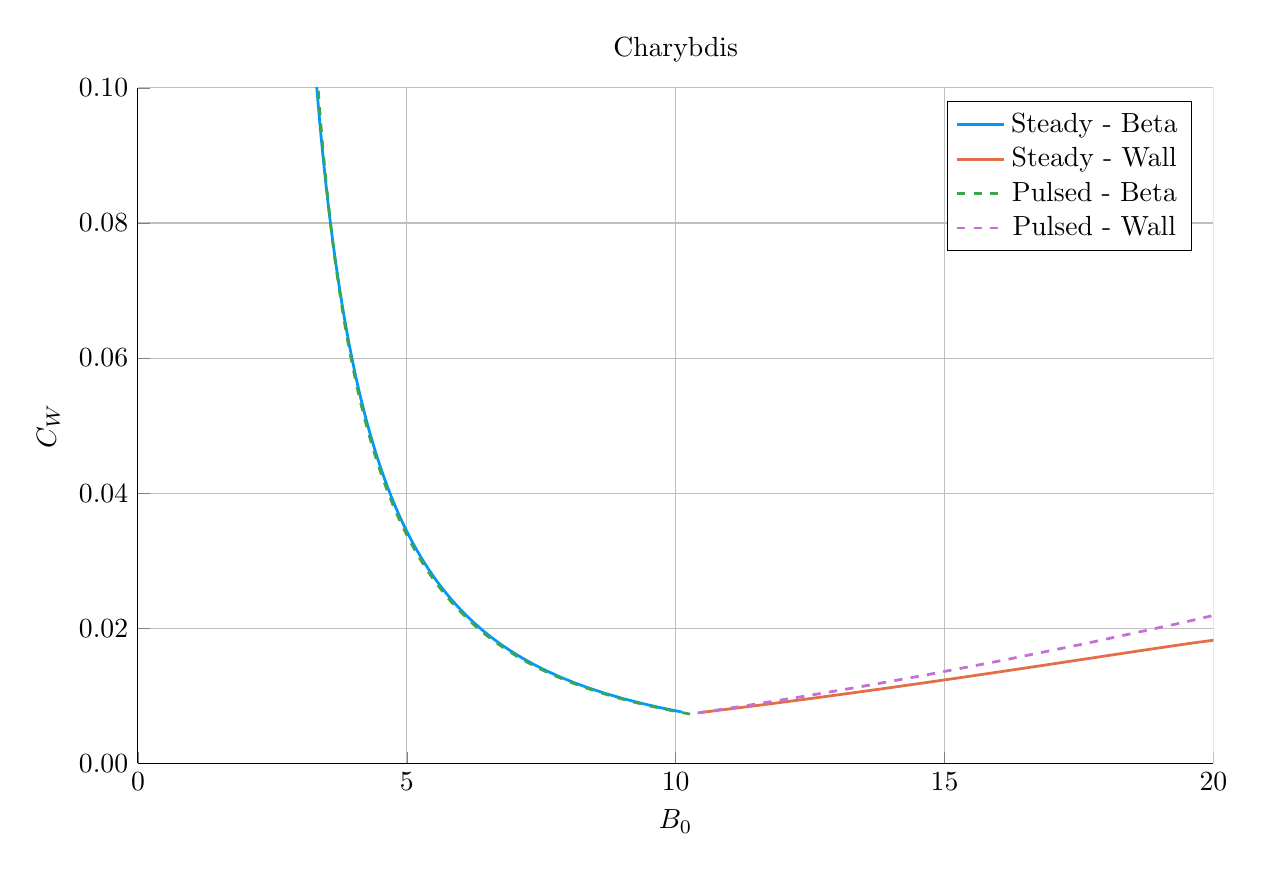
\begin{tikzpicture}[]
\begin{axis}[height = {101.6mm}, ylabel = {${C}_{W}$}, title = {Charybdis}, xmin = {0.0}, xmax = {20.0}, ymax = {0.1}, xlabel = {${B}_{0}$}, {unbounded coords=jump, scaled x ticks = false, xticklabel style={rotate = 0}, xmajorgrids = true, xtick = {0.0,5.0,10.0,15.0,20.0}, xticklabels = {0,5,10,15,20}, xtick align = inside, axis lines* = left, scaled y ticks = false, yticklabel style={rotate = 0}, ymajorgrids = true, ytick = {0.0,0.02,0.04,0.06,0.08,0.1}, yticklabels = {0.00,0.02,0.04,0.06,0.08,0.10}, ytick align = inside, axis lines* = left,     xshift = 0.0mm,
    yshift = 0.0mm,
    axis background/.style={fill={rgb,1:red,1.00000000;green,1.00000000;blue,1.00000000}}
, colorbar style={title=}}, ymin = {0.0}, width = {152.4mm}]\addplot+ [color = {rgb,1:red,0.00000000;green,0.60560316;blue,0.97868012},
draw opacity=1.0,
line width=1,
solid,mark = none,
mark size = 2.0,
mark options = {
    color = {rgb,1:red,0.00000000;green,0.00000000;blue,0.00000000}, draw opacity = 1.0,
    fill = {rgb,1:red,0.00000000;green,0.60560316;blue,0.97868012}, fill opacity = 1.0,
    line width = 1,
    rotate = 0,
    solid
}]coordinates {
(10.112818033153026, 0.007598383414978856)
(9.722156888543116, 0.008230424223188452)
(9.357875603858393, 0.008896404207575682)
(9.017653755630063, 0.009597023567402527)
(8.6995124437054, 0.010332804662622194)
(8.401566530516865, 0.011104394978990672)
(8.122163706328223, 0.011912345200844093)
(7.859819415455661, 0.012757161102175962)
(7.613196557650265, 0.013639302343912054)
(7.381088038653343, 0.014559181429827196)
(7.162401716104116, 0.015517162820285028)
(6.956147367527331, 0.016513562202290014)
(6.761425371986388, 0.017548645913683623)
(6.577416849463348, 0.018622630518712633)
(6.403375044688587, 0.019735682531644493)
(6.2386177769852695, 0.02088791828458706)
(6.0825208065966905, 0.022079403933712667)
(5.934511989185341, 0.02331015560822712)
(5.794066116682695, 0.024580139674436858)
(5.660700347012839, 0.02588927313954039)
(5.533970150598111, 0.027237424167073223)
(5.413465705416883, 0.02862441270831249)
(5.298808685607224, 0.03005001123436344)
(5.189649392059402, 0.031513945582432444)
(5.085664187259174, 0.033015895883282464)
(4.986553195072601, 0.03455549758379169)
(4.892038235455667, 0.03613234255000151)
(4.801860966679364, 0.037745980245626594)
(4.7157812114040425, 0.03939591897965519)
(4.633575445956479, 0.041081627216715676)
(4.5550354347559185, 0.04280253494397791)
(4.479966994069385, 0.04455803508845128)
(4.408188871204256, 0.046347484978679)
(4.33953172691477, 0.048170207844964834)
(4.273837210246432, 0.05002549435242988)
(4.210957116299974, 0.051912604161371986)
(4.15075261849161, 0.053830767509593334)
(4.0930935678432965, 0.05577918681155204)
(4.037857852672517, 0.05775703826940529)
(3.9849308127842145, 0.05976347349121981)
(3.9342047029103653, 0.06179762111185749)
(3.8855782007091695, 0.06385858841225403)
(3.838955955133626, 0.06594546293303978)
(3.7942481714200484, 0.06805731407868133)
(3.7513702293348077, 0.07019319470855978)
(3.710242331663442, 0.07235214271160313)
(3.6707891802306123, 0.0745331825613442)
(3.6329396770109583, 0.07673532684849063)
(3.5966266481325166, 0.07895757778829673)
(3.5617865887889004, 0.08119892870027327)
(3.5283594272686503, 0.08345836545794902)
(3.496288306480746, 0.08573486790664452)
(3.465519381509793, 0.08802741124736263)
(3.4360016318699595, 0.09033496738515884)
(3.4076866872513096, 0.0926565062404898)
(3.380528665662031, 0.09499099702224018)
(3.3544840229690007, 0.09733740946131986)
(3.3295114129297314, 0.09969471500383864)
(3.3055715568879336, 0.10206188796308927)
(3.2826271223788512, 0.10443790662966322)
(3.260642607548369, 0.10682175444066445)
(3.239584247604666, 0.10921242049746493)
(3.2194198921826622, 0.11160890156230109)
(3.2001189373344725, 0.11401020198268878)
(3.181652227422265, 0.11641533509457672)
(3.163991977015565, 0.11882332397376366)
(3.1471116955378684, 0.12123320224599504)
(3.130986116696265, 0.12364401485456963)
(3.115591132350856, 0.1260548187858383)
(3.1009037305081053, 0.12846468375306214)
(3.0869019371473265, 0.13087269283917113)
(3.0735647616124355, 0.13327794309901428)
(3.0608721453218655, 0.13567954612178545)
};
\addlegendentry{Steady - Beta}
\addplot+ [color = {rgb,1:red,0.88887350;green,0.43564919;blue,0.27812294},
draw opacity=1.0,
line width=1,
solid,mark = none,
mark size = 2.0,
mark options = {
    color = {rgb,1:red,0.00000000;green,0.00000000;blue,0.00000000}, draw opacity = 1.0,
    fill = {rgb,1:red,0.88887350;green,0.43564919;blue,0.27812294}, fill opacity = 1.0,
    line width = 1,
    rotate = 0,
    solid
}]coordinates {
(20.758867641064707, 0.018765308409143346)
(20.346250098246923, 0.018594952760163406)
(19.57104597888471, 0.01777146918538113)
(18.681781921115476, 0.016727851446155666)
(17.775790175980152, 0.015638576778075435)
(16.896654716492492, 0.014581653280825104)
(16.063927450323227, 0.013591211730165224)
(15.285557510665852, 0.012680275903338053)
(14.563500533069154, 0.01185123263968419)
(13.896568848875791, 0.01110114677254841)
(13.281970890030232, 0.010424581221258129)
(12.716170469467318, 0.009815118917575654)
(12.195372283741088, 0.00926617943914564)
(11.715794270833433, 0.008771443174384838)
(11.273815669498969, 0.008325054959037046)
(10.866051794088186, 0.007921704192505699)
(10.489365023931143, 0.007556609136513177)
};
\addlegendentry{Steady - Wall}
\addplot+ [color = {rgb,1:red,0.24222430;green,0.64327509;blue,0.30444865},
draw opacity=1.0,
line width=1,
dashed,mark = none,
mark size = 2.0,
mark options = {
    color = {rgb,1:red,0.00000000;green,0.00000000;blue,0.00000000}, draw opacity = 1.0,
    fill = {rgb,1:red,0.24222430;green,0.64327509;blue,0.30444865}, fill opacity = 1.0,
    line width = 1,
    rotate = 0,
    solid
}]coordinates {
(10.26788634689966, 0.007291637162809203)
(9.953967652326213, 0.007763018579561715)
(9.567926244368271, 0.008410560830066265)
(9.207974394987358, 0.009093056690349528)
(8.871841888699304, 0.009811202030777346)
(8.557505525932248, 0.010565644256199823)
(8.263156925406376, 0.01135697964954635)
(7.9871752024348766, 0.01218575089778548)
(7.728103682045175, 0.013052444820635726)
(7.484629973620137, 0.01395749030938975)
(7.255568856523303, 0.014901256485610468)
(7.039847526735421, 0.015884051087442074)
(6.836492834698909, 0.01690611908975986)
(6.644620209081183, 0.01796764156282338)
(6.463424013335149, 0.01906873477252413)
(6.2921691243175495, 0.020209449523749864)
(6.13018355681404, 0.02138977074682875)
(5.97685198655569, 0.022609617323612653)
(5.831610044919842, 0.023868842161338135)
(5.693939286027163, 0.025167232481888336)
(5.563362729090489, 0.026504510357656302)
(5.439440906144732, 0.0278803334592314)
(5.321768347746793, 0.02929429601917866)
(5.209970453003084, 0.030745929990983068)
(5.103700692769835, 0.03223470641747899)
(5.002638109938164, 0.03376003696406285)
(4.906485077678376, 0.03532127563010485)
(4.814965286571576, 0.03691772061565451)
(4.727821933804548, 0.03854861633202897)
(4.644816091323922, 0.04021315554278132)
(4.565725232806084, 0.04191048162126061)
(4.490341901840154, 0.04363969091085349)
(4.418472505906755, 0.04539983517396531)
(4.349936222622964, 0.047189924115870814)
(4.284564006352339, 0.049008927969770806)
(4.222197684694192, 0.05085578012965056)
(4.162689135592264, 0.05272937981792158)
(4.105899536872315, 0.05462859477526984)
(4.051698680949713, 0.056552263960658246)
(3.9999643482627323, 0.058499200250012214)
(3.9505817337017928, 0.06046819312273483)
(3.903442920928527, 0.062458011325916454)
(3.858446400032002, 0.06446740550676137)
(3.8154966244515616, 0.06649511080452623)
(3.7745036035252744, 0.06853984939399767)
(3.7353825273991994, 0.07060033297331114)
(3.6980534213689746, 0.07267526518964869)
(3.6624408270205375, 0.07476334399712868)
(3.62847350780097, 0.07686326394192533)
(3.5960841768845415, 0.07897371837037194)
(3.565209245407392, 0.08109340155652811)
(3.5357885893311605, 0.0832210107463015)
(3.5077653333614305, 0.08535524811591486)
(3.4810856504959875, 0.08749482264305544)
(3.4556985759109375, 0.08963845188964095)
(3.4315558340122845, 0.09178486369563649)
(3.408611677587535, 0.09393279778385825)
(3.3868227380888998, 0.09608100727612065)
(3.36614788616562, 0.09822826012150637)
(3.3465481016421226, 0.10037334043786662)
(3.327986352208224, 0.1025150497680155)
(3.3104274769652595, 0.10465220838353721)
(3.2938380965241474, 0.1067836557197021)
(3.278186482171801, 0.10890825269906537)
(3.263442495132517, 0.11102488135374605)
(3.2495774839156075, 0.1131324463411963)
(3.236564206241785, 0.11522987560063444)
(3.224376752844934, 0.11731612107126856)
(3.212990475972638, 0.11939015934381376)
(3.2023819222517877, 0.12145099224802183)
(3.192528769611062, 0.12349764737898258)
(3.1834097679780142, 0.1255291785649034)
(3.1750046834890777, 0.12754466627907632)
(3.1672942459724482, 0.12954321799866983)
};
\addlegendentry{Pulsed - Beta}
\addplot+ [color = {rgb,1:red,0.76444018;green,0.44411178;blue,0.82429754},
draw opacity=1.0,
line width=1,
dashed,mark = none,
mark size = 2.0,
mark options = {
    color = {rgb,1:red,0.00000000;green,0.00000000;blue,0.00000000}, draw opacity = 1.0,
    fill = {rgb,1:red,0.76444018;green,0.44411178;blue,0.82429754}, fill opacity = 1.0,
    line width = 1,
    rotate = 0,
    solid
}]coordinates {
(48.990476413653056, 0.09724163307501366)
(42.83950920694117, 0.07766994779263652)
(37.687790427214495, 0.06269593244609177)
(33.33937742845888, 0.05109841711622891)
(29.64296398154308, 0.04201539110057761)
(26.48039367255613, 0.034828857187910324)
(23.758442882319894, 0.029089432591006322)
(21.402860298405816, 0.02446606951047545)
(19.353987387634486, 0.020711961258999954)
(17.563502020363714, 0.017641064746807725)
(15.991970371213752, 0.015111701839397276)
(14.606987499719377, 0.013014953187280779)
(13.381751501116137, 0.011266342778060628)
(12.293960329570087, 0.009799811915435606)
(11.32495111804522, 0.00856330563618739)
(10.459023415380802, 0.007515507834648486)
(10.26788634689966, 0.007291637162809203)
};
\addlegendentry{Pulsed - Wall}
\end{axis}

\end{tikzpicture}

		\end{adjustbox}
        \caption{Charybdis}
    \end{subfigure}
    \hfill
    \begin{subfigure}[t]{0.45\textwidth}
        \centering
		\begin{adjustbox}{width=\textwidth}
			\Large
			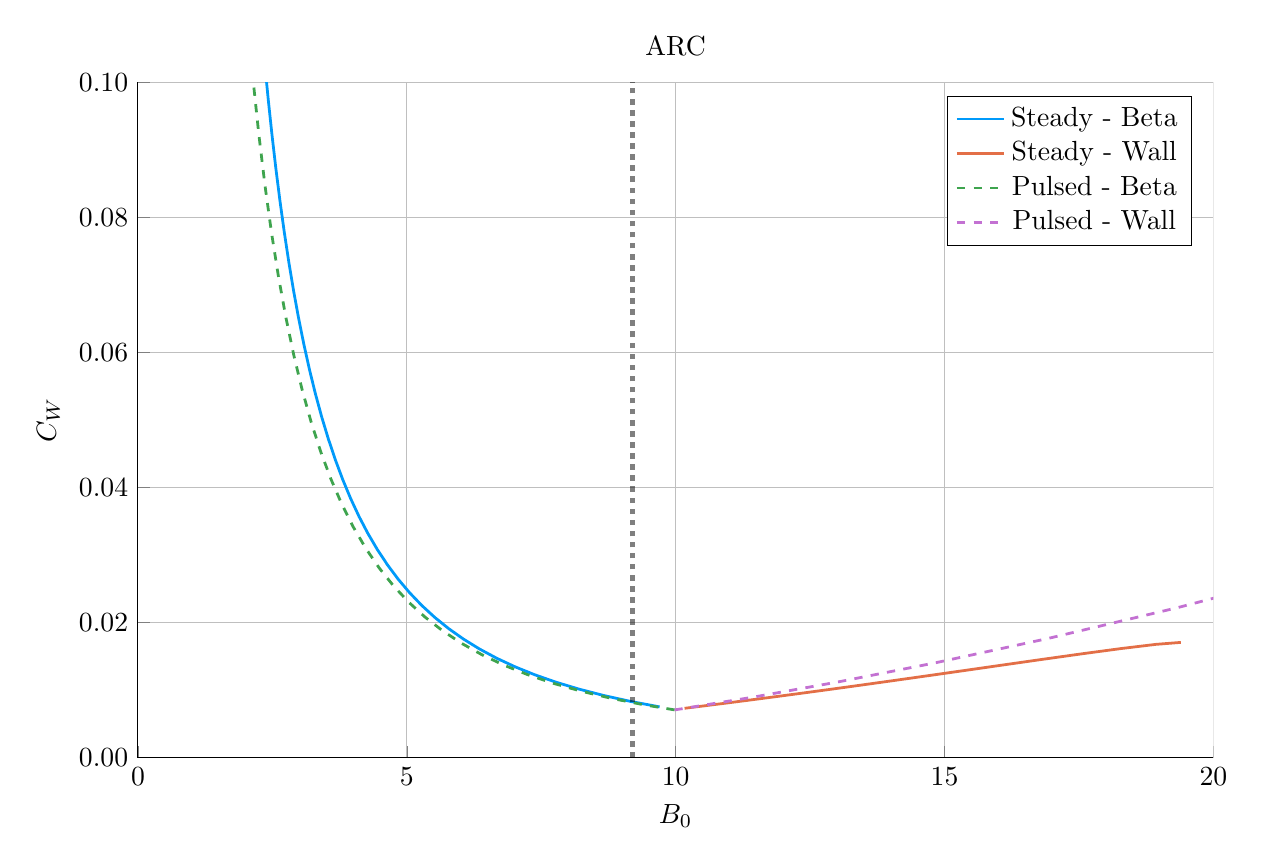
\begin{tikzpicture}[]
\begin{axis}[height = {101.6mm}, ylabel = {${C}_{W}$}, title = {ARC}, xmin = {0.0}, xmax = {20.0}, ymax = {0.1}, xlabel = {${B}_{0}$}, {unbounded coords=jump, scaled x ticks = false, xticklabel style={rotate = 0}, xmajorgrids = true, xtick = {0.0,5.0,10.0,15.0,20.0}, xticklabels = {0,5,10,15,20}, xtick align = inside, axis lines* = left, scaled y ticks = false, yticklabel style={rotate = 0}, ymajorgrids = true, ytick = {0.0,0.02,0.04,0.06,0.08,0.1}, yticklabels = {0.00,0.02,0.04,0.06,0.08,0.10}, ytick align = inside, axis lines* = left,     xshift = 0.0mm,
    yshift = 0.0mm,
    axis background/.style={fill={rgb,1:red,1.00000000;green,1.00000000;blue,1.00000000}}
, colorbar style={title=}}, ymin = {0.0}, width = {152.4mm}]\addplot+ [color = {rgb,1:red,0.00000000;green,0.60560316;blue,0.97868012},
draw opacity=1.0,
line width=1,
solid,mark = none,
mark size = 2.0,
mark options = {
    color = {rgb,1:red,0.00000000;green,0.00000000;blue,0.00000000}, draw opacity = 1.0,
    fill = {rgb,1:red,0.00000000;green,0.60560316;blue,0.97868012}, fill opacity = 1.0,
    line width = 1,
    rotate = 0,
    solid
}]coordinates {
(9.701206080853105, 0.00751651377736839)
(9.162315904693079, 0.008323905812934898)
(8.664301107137337, 0.009198905086222158)
(8.203576462497304, 0.010145151644824739)
(7.776718537485166, 0.011166668317960562)
(7.380720231870917, 0.012267478183796882)
(7.012886014999712, 0.013451673110529961)
(6.670795005901889, 0.014723405583659413)
(6.352268997292712, 0.01608688012694734)
(6.055344682097163, 0.017546344352390175)
(5.778249464564785, 0.019106079676451882)
(5.519380338856715, 0.020770391741442663)
(5.2772854007125325, 0.02254360058225732)
(5.050647625972996, 0.02443003057971548)
(4.838270606140816, 0.026434000242494555)
(4.639065978019038, 0.028559811860080504)
(4.4520423235376105, 0.030811741069328453)
(4.276295348572609, 0.03319402637711819)
(4.110999177018484, 0.03571085868120887)
(3.9553986195015125, 0.038366370830779505)
(3.8088022956698633, 0.041164627267286334)
(3.6705765055641186, 0.04410961378519341)
(3.54013975965751, 0.047205227450858)
(3.4169578891619192, 0.050455266716399376)
(3.30053966845824, 0.05386342176374704)
(3.1904328903033052, 0.05743326511231589)
(3.086220842019516, 0.061168242521834885)
(2.9875191373772063, 0.0650716642198721)
(2.8939728644914635, 0.0691466964814904)
(2.8052540149097247, 0.07339635358630757)
(2.7210591632720242, 0.07782349017600093)
(2.6411073705789065, 0.08243079403304142)
(2.565138287279709, 0.08722077929915266)
(2.492910435164382, 0.09219578014969385)
(2.4241996494611984, 0.09735794493788336)
(2.3587976646588236, 0.10270923082049731)
(2.296510829425685, 0.10825139887447487)
(2.237158937627476, 0.11398600971161459)
(2.180574163874242, 0.11991441959647205)
(2.126600093288366, 0.1260377770704313)
(2.075090836295778, 0.1323570200829707)
(2.0259102202234582, 0.13887287362917833)
(1.978931050353818, 0.14558584789074455)
(1.9340344338545452, 0.15249623687593467)
(1.8911091606836798, 0.1596041175523241)
(1.8500511361739687, 0.16690934946459546)
(1.8107628605384507, 0.17441157482817518)
(1.773152951016952, 0.1821102190881948)
(1.7371357028100902, 0.19000449193192903)
(1.7026306853269466, 0.19809338874181076)
(1.6695623706125668, 0.2063756924750063)
(1.6378597911249178, 0.21484997595463062)
(1.607456224302725, 0.22351460455684893)
(1.5782889016090462, 0.23236773927733403)
(1.5502987399539199, 0.24140734015998855)
(1.5234300935954943, 0.2506311700702061)
(1.4976305247952577, 0.26003679879456143)
(1.4728505916614916, 0.26962160744844355)
(1.4490436517578602, 0.2793827931728701)
(1.4261656801829077, 0.2893173741014787)
};
\addlegendentry{Steady - Beta}
\addplot+ [color = {rgb,1:red,0.88887350;green,0.43564919;blue,0.27812294},
draw opacity=1.0,
line width=1,
solid,mark = none,
mark size = 2.0,
mark options = {
    color = {rgb,1:red,0.00000000;green,0.00000000;blue,0.00000000}, draw opacity = 1.0,
    fill = {rgb,1:red,0.88887350;green,0.43564919;blue,0.27812294}, fill opacity = 1.0,
    line width = 1,
    rotate = 0,
    solid
}]coordinates {
(19.394007482712425, 0.017062717610395756)
(18.932196567189358, 0.01677318247708789)
(18.296989378345195, 0.01616608087020061)
(17.587029315408756, 0.015409201334794807)
(16.847882407994106, 0.014583614099307054)
(16.111374502564406, 0.01374625755936427)
(15.396027314547156, 0.012930331454144767)
(14.710952688793137, 0.012152313568351602)
(14.06168447794857, 0.011421914699879928)
(13.450465418483889, 0.010742972750322424)
(12.877644538645335, 0.010115989865118968)
(12.342394470642008, 0.009539468548127306)
(11.843182246608265, 0.00901077532361949)
(11.376441269625893, 0.008524384373336923)
(10.944966372727551, 0.008083786116178366)
(10.541663878705513, 0.007678592362816001)
(10.165908182236457, 0.0073076305932358344)
};
\addlegendentry{Steady - Wall}
\addplot+ [color = {rgb,1:red,0.24222430;green,0.64327509;blue,0.30444865},
draw opacity=1.0,
line width=1,
dashed,mark = none,
mark size = 2.0,
mark options = {
    color = {rgb,1:red,0.00000000;green,0.00000000;blue,0.00000000}, draw opacity = 1.0,
    fill = {rgb,1:red,0.24222430;green,0.64327509;blue,0.30444865}, fill opacity = 1.0,
    line width = 1,
    rotate = 0,
    solid
}]coordinates {
(9.980483622051658, 0.007070839678110688)
(9.392786903460065, 0.007852618677281367)
(8.79273598103983, 0.008801125480455354)
(8.23820290909994, 0.009848957316818736)
(7.725182218401588, 0.011005021009379608)
(7.250078106370205, 0.012278877224830715)
(6.80965553466646, 0.013680774995781924)
(6.400998063035608, 0.01522168706241675)
(6.0214713600430425, 0.01691334607316053)
(5.668691517461799, 0.01876828173242221)
(5.340497445229901, 0.020799859050557753)
(5.034926745580058, 0.02302231794191222)
(4.750194564008521, 0.02545081453735327)
(4.484674995755211, 0.028101464735781394)
(4.236884692979903, 0.030991390724248)
(4.00546837264544, 0.03413877146046793)
(3.7891859704718387, 0.03756289844971818)
(3.5869012239550364, 0.04128423857957625)
(3.3975714987448393, 0.04532450632539042)
(3.2202386987489797, 0.04970674833925621)
(3.0540211220494466, 0.05445544432876858)
(2.8981061427709687, 0.059596629277403584)
(2.7517436139566023, 0.06515804353669719)
(2.6142398986781377, 0.07116931924441194)
(2.4849524463010138, 0.07766221405391976)
(2.363284838174807, 0.08467090653190464)
(2.248682232019848, 0.09223237213933476)
(2.140627136740878, 0.10038686497222395)
(2.038635448877246, 0.10917853919500715)
(1.9422526775794744, 0.11865625658225108)
(1.8510502754751532, 0.12887464475233826)
(1.7646219756564088, 0.1398954977169483)
(1.6825800061969869, 0.15178965160557917)
(1.6045510059627948, 0.16463953300974782)
(1.53017138625397, 0.17854268160508957)
(1.4590817483192686, 0.19361672262027943)
(1.3909197311384796, 0.21000656636649426)
(1.3253102336217724, 0.22789515931839086)
(1.261851128383913, 0.24752015854836598)
(1.20009089049112, 0.2692010388315911)
(1.1394908096975784, 0.2933858656724498)
};
\addlegendentry{Pulsed - Beta}
\addplot+ [color = {rgb,1:red,0.76444018;green,0.44411178;blue,0.82429754},
draw opacity=1.0,
line width=1,
dashed,mark = none,
mark size = 2.0,
mark options = {
    color = {rgb,1:red,0.00000000;green,0.00000000;blue,0.00000000}, draw opacity = 1.0,
    fill = {rgb,1:red,0.76444018;green,0.44411178;blue,0.82429754}, fill opacity = 1.0,
    line width = 1,
    rotate = 0,
    solid
}]coordinates {
(29.27715761652869, 0.045433420664911836)
(25.4410619834368, 0.0356668159806907)
(22.158819835998365, 0.02810552804100701)
(19.342453256965573, 0.02222656993153558)
(16.919364280634177, 0.0176372518175528)
(14.829378672669455, 0.014041066675248008)
(13.022412368922526, 0.011212962182114766)
(11.456617692058645, 0.00898128637894181)
(10.096901921254785, 0.00721451699843558)
(9.980483622051658, 0.007070839678110688)
};
\addlegendentry{Pulsed - Wall}
\addplot+ [color = {rgb,1:red,0.00000000;green,0.00000000;blue,0.00000000},
draw opacity=0.5,
line width=2,
dotted,mark = none,
mark size = 2.0,
mark options = {
    color = {rgb,1:red,0.00000000;green,0.00000000;blue,0.00000000}, draw opacity = 0.5,
    fill = {rgb,1:red,0.00000000;green,0.00000000;blue,0.00000000}, fill opacity = 0.5,
    line width = 1,
    rotate = 0,
    solid
},forget plot]coordinates {
(0.0, NaN)
(20.0, NaN)
};
\addplot+ [color = {rgb,1:red,0.00000000;green,0.00000000;blue,0.00000000},
draw opacity=0.5,
line width=2,
dotted,mark = none,
mark size = 2.0,
mark options = {
    color = {rgb,1:red,0.00000000;green,0.00000000;blue,0.00000000}, draw opacity = 0.5,
    fill = {rgb,1:red,0.00000000;green,0.00000000;blue,0.00000000}, fill opacity = 0.5,
    line width = 1,
    rotate = 0,
    solid
},forget plot]coordinates {
(9.2, 0.0)
(9.2, 0.1)
};
\addplot+[draw=none, color = {rgb,1:red,0.00000000;green,0.00000000;blue,0.00000000},
draw opacity=0.5,
line width=0,
solid,mark = *,
mark size = 2.0,
mark options = {
    color = {rgb,1:red,0.00000000;green,0.00000000;blue,0.00000000}, draw opacity = 0.5,
    fill = {rgb,1:red,0.00000000;green,0.00000000;blue,0.00000000}, fill opacity = 0.5,
    line width = 1,
    rotate = 0,
    solid
},forget plot] coordinates {
(9.2, NaN)
};
\end{axis}

\end{tikzpicture}

		\end{adjustbox}
        \caption{ARC}
    \end{subfigure}
    \hfill \hfill ~\\ ~\\ ~\\ ~\\
    \hfill
    \begin{subfigure}[t]{0.45\textwidth}
        \centering
		\begin{adjustbox}{width=\textwidth}
			\Large
			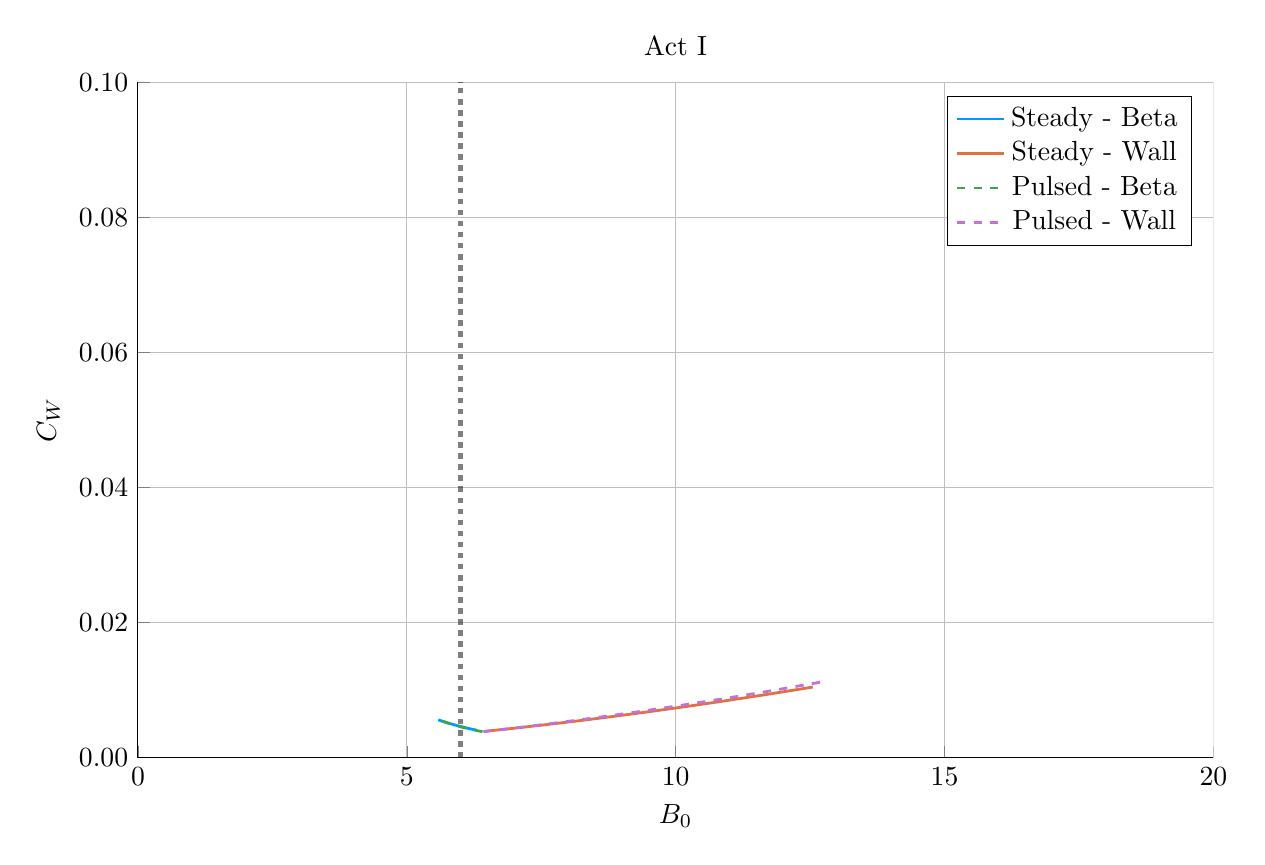
\begin{tikzpicture}[]
\begin{axis}[height = {101.6mm}, ylabel = {${C}_{W}$}, title = {Act I}, xmin = {0.0}, xmax = {20.0}, ymax = {0.1}, xlabel = {${B}_{0}$}, {unbounded coords=jump, scaled x ticks = false, xticklabel style={rotate = 0}, xmajorgrids = true, xtick = {0.0,5.0,10.0,15.0,20.0}, xticklabels = {0,5,10,15,20}, xtick align = inside, axis lines* = left, scaled y ticks = false, yticklabel style={rotate = 0}, ymajorgrids = true, ytick = {0.0,0.02,0.04,0.06,0.08,0.1}, yticklabels = {0.00,0.02,0.04,0.06,0.08,0.10}, ytick align = inside, axis lines* = left,     xshift = 0.0mm,
    yshift = 0.0mm,
    axis background/.style={fill={rgb,1:red,1.00000000;green,1.00000000;blue,1.00000000}}
, colorbar style={title=}}, ymin = {0.0}, width = {152.4mm}]\addplot+ [color = {rgb,1:red,0.00000000;green,0.60560316;blue,0.97868012},
draw opacity=1.0,
line width=1,
solid,mark = none,
mark size = 2.0,
mark options = {
    color = {rgb,1:red,0.00000000;green,0.00000000;blue,0.00000000}, draw opacity = 1.0,
    fill = {rgb,1:red,0.00000000;green,0.60560316;blue,0.97868012}, fill opacity = 1.0,
    line width = 1,
    rotate = 0,
    solid
}]coordinates {
(6.30336807958207, 0.004055552148042579)
(6.162193069273141, 0.004300298316165893)
(6.030717178404645, 0.004550498291731095)
(5.908065509576601, 0.004805976791051415)
(5.793464904530972, 0.005066558265934883)
(5.686229631357383, 0.005332067188485748)
(5.585749511271037, 0.005602328191394613)
};
\addlegendentry{Steady - Beta}
\addplot+ [color = {rgb,1:red,0.88887350;green,0.43564919;blue,0.27812294},
draw opacity=1.0,
line width=1,
solid,mark = none,
mark size = 2.0,
mark options = {
    color = {rgb,1:red,0.00000000;green,0.00000000;blue,0.00000000}, draw opacity = 1.0,
    fill = {rgb,1:red,0.88887350;green,0.43564919;blue,0.27812294}, fill opacity = 1.0,
    line width = 1,
    rotate = 0,
    solid
}]coordinates {
(12.549536249695134, 0.010450364750783054)
(11.658754653696462, 0.009311160177277214)
(10.883719833507003, 0.008367979762533702)
(10.206258129789394, 0.007581000508027489)
(9.611335769312953, 0.0069194030019139735)
(9.086446934250878, 0.006359119854353646)
(8.62129895070743, 0.0058814059200114925)
(8.207216040989662, 0.005471332591600982)
(7.837119555085499, 0.005117248050094358)
(7.505047858717157, 0.00480979217186778)
(7.20604322925957, 0.0045414928704811935)
(6.935884710193303, 0.0043062495703983395)
(6.691016583192173, 0.004099109819554263)
(6.468415485086983, 0.0039160098791423655)
};
\addlegendentry{Steady - Wall}
\addplot+ [color = {rgb,1:red,0.24222430;green,0.64327509;blue,0.30444865},
draw opacity=1.0,
line width=1,
dashed,mark = none,
mark size = 2.0,
mark options = {
    color = {rgb,1:red,0.00000000;green,0.00000000;blue,0.00000000}, draw opacity = 1.0,
    fill = {rgb,1:red,0.24222430;green,0.64327509;blue,0.30444865}, fill opacity = 1.0,
    line width = 1,
    rotate = 0,
    solid
}]coordinates {
(6.408263337806559, 0.003837054084878144)
(6.408263337806564, 0.0038370540848781357)
(6.385466513301022, 0.003872993818821736)
(6.245492502072912, 0.004106512578517519)
(6.116010320461132, 0.004344317387601225)
(5.9960421481916395, 0.004586160922256416)
(5.884727159112828, 0.004831799090393476)
(5.781304768121868, 0.00508099132781059)
(5.685100648450046, 0.005333500860613775)
(5.595515000321003, 0.005589094940610307)
};
\addlegendentry{Pulsed - Beta}
\addplot+ [color = {rgb,1:red,0.76444018;green,0.44411178;blue,0.82429754},
draw opacity=1.0,
line width=1,
dashed,mark = none,
mark size = 2.0,
mark options = {
    color = {rgb,1:red,0.00000000;green,0.00000000;blue,0.00000000}, draw opacity = 1.0,
    fill = {rgb,1:red,0.76444018;green,0.44411178;blue,0.82429754}, fill opacity = 1.0,
    line width = 1,
    rotate = 0,
    solid
}]coordinates {
(12.684248532650473, 0.011163257244949718)
(11.66307871570063, 0.009745831059904)
(10.781888309639141, 0.008590800927445573)
(10.016282491385791, 0.007639361749178777)
(9.346943280276514, 0.006847895899781745)
(8.758420158941194, 0.0061835958355957316)
(8.238241792953433, 0.005621466066992172)
(7.776255600865612, 0.005142236201168238)
(7.364131118520045, 0.0047308861724008975)
(6.994982564641668, 0.00437558945422717)
(6.66307916140573, 0.004066945929726434)
(6.408263337806559, 0.003837054084878144)
(6.408263337806564, 0.0038370540848781357)
};
\addlegendentry{Pulsed - Wall}
\addplot+ [color = {rgb,1:red,0.00000000;green,0.00000000;blue,0.00000000},
draw opacity=0.5,
line width=2,
dotted,mark = none,
mark size = 2.0,
mark options = {
    color = {rgb,1:red,0.00000000;green,0.00000000;blue,0.00000000}, draw opacity = 0.5,
    fill = {rgb,1:red,0.00000000;green,0.00000000;blue,0.00000000}, fill opacity = 0.5,
    line width = 1,
    rotate = 0,
    solid
},forget plot]coordinates {
(0.0, NaN)
(20.0, NaN)
};
\addplot+ [color = {rgb,1:red,0.00000000;green,0.00000000;blue,0.00000000},
draw opacity=0.5,
line width=2,
dotted,mark = none,
mark size = 2.0,
mark options = {
    color = {rgb,1:red,0.00000000;green,0.00000000;blue,0.00000000}, draw opacity = 0.5,
    fill = {rgb,1:red,0.00000000;green,0.00000000;blue,0.00000000}, fill opacity = 0.5,
    line width = 1,
    rotate = 0,
    solid
},forget plot]coordinates {
(6.0, 0.0)
(6.0, 0.1)
};
\addplot+[draw=none, color = {rgb,1:red,0.00000000;green,0.00000000;blue,0.00000000},
draw opacity=0.5,
line width=0,
solid,mark = *,
mark size = 2.0,
mark options = {
    color = {rgb,1:red,0.00000000;green,0.00000000;blue,0.00000000}, draw opacity = 0.5,
    fill = {rgb,1:red,0.00000000;green,0.00000000;blue,0.00000000}, fill opacity = 0.5,
    line width = 1,
    rotate = 0,
    solid
},forget plot] coordinates {
(6.0, NaN)
};
\end{axis}

\end{tikzpicture}

		\end{adjustbox}
        \caption{ACT I}
    \end{subfigure}
    \hfill
    \begin{subfigure}[t]{0.45\textwidth}
        \centering
		\begin{adjustbox}{width=\textwidth}
			\Large
			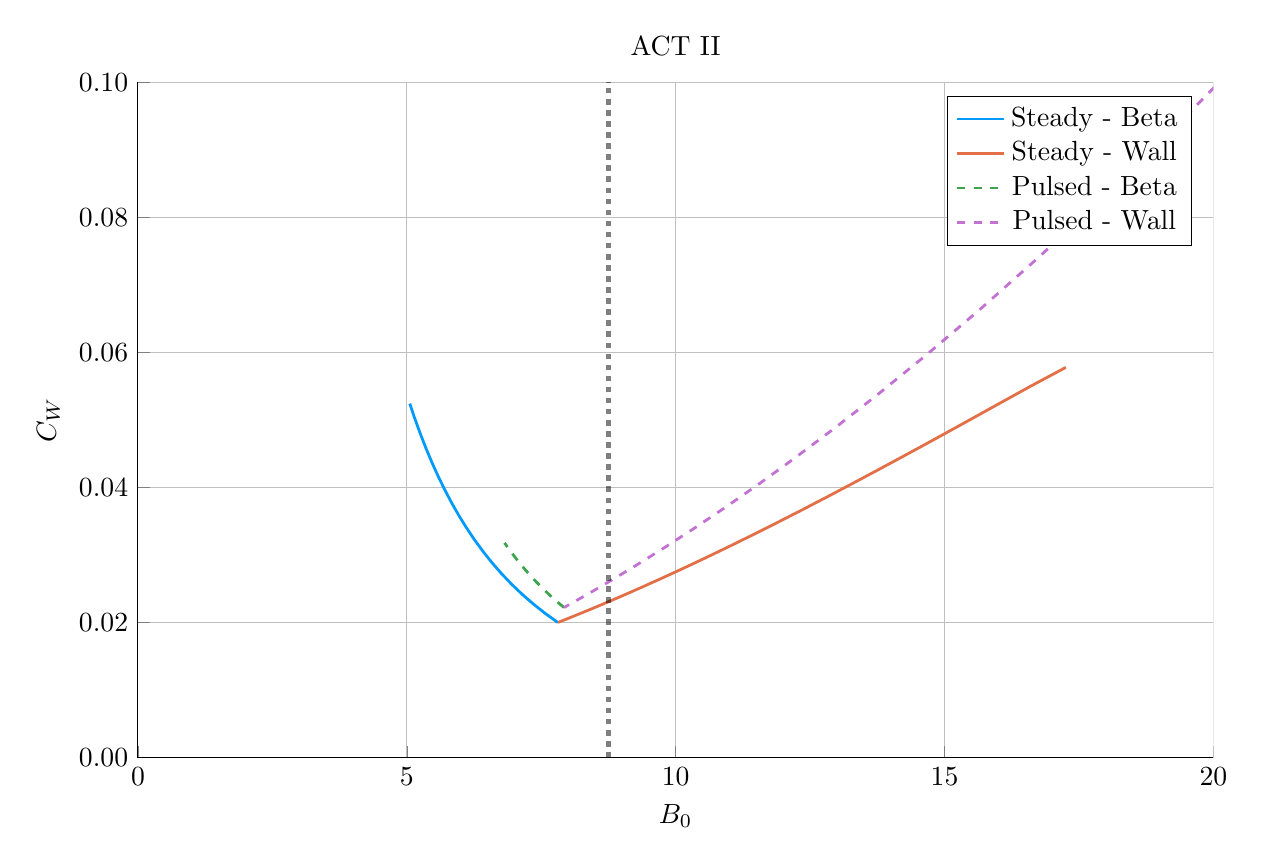
\begin{tikzpicture}[]
\begin{axis}[height = {101.6mm}, ylabel = {${C}_{W}$}, title = {ACT II}, xmin = {0.0}, xmax = {20.0}, ymax = {0.1}, xlabel = {${B}_{0}$}, {unbounded coords=jump, scaled x ticks = false, xticklabel style={rotate = 0}, xmajorgrids = true, xtick = {0.0,5.0,10.0,15.0,20.0}, xticklabels = {0,5,10,15,20}, xtick align = inside, axis lines* = left, scaled y ticks = false, yticklabel style={rotate = 0}, ymajorgrids = true, ytick = {0.0,0.02,0.04,0.06,0.08,0.1}, yticklabels = {0.00,0.02,0.04,0.06,0.08,0.10}, ytick align = inside, axis lines* = left,     xshift = 0.0mm,
    yshift = 0.0mm,
    axis background/.style={fill={rgb,1:red,1.00000000;green,1.00000000;blue,1.00000000}}
, colorbar style={title=}}, ymin = {0.0}, width = {152.4mm}]\addplot+ [color = {rgb,1:red,0.00000000;green,0.60560316;blue,0.97868012},
draw opacity=1.0,
line width=1,
solid,mark = none,
mark size = 2.0,
mark options = {
    color = {rgb,1:red,0.00000000;green,0.00000000;blue,0.00000000}, draw opacity = 1.0,
    fill = {rgb,1:red,0.00000000;green,0.60560316;blue,0.97868012}, fill opacity = 1.0,
    line width = 1,
    rotate = 0,
    solid
}]coordinates {
(7.810935944285959, 0.019999870342781445)
(7.57736049850867, 0.02133467083845229)
(7.354864292609041, 0.022732819748494743)
(7.145167234136329, 0.024185030975062572)
(6.9473303865083675, 0.025691491983248542)
(6.760499508614096, 0.027252320661142464)
(6.583897990324067, 0.028867554534578326)
(6.416817229618043, 0.030537157829042417)
(6.258609820663305, 0.032261020375438675)
(6.108683264880386, 0.034038958296321455)
(5.966494431410919, 0.03587071487617403)
(5.831544666176381, 0.0377559616009066)
(5.703375459679132, 0.03969429938840844)
(5.581564609582325, 0.04168525992229865)
(5.465722802994068, 0.04372830718110872)
(5.355490573482678, 0.04582283908419109)
(5.25053558682053, 0.047968189231402746)
(5.1505502068221745, 0.0501636288266544)
(5.0552493196883175, 0.0524083686363995)
};
\addlegendentry{Steady - Beta}
\addplot+ [color = {rgb,1:red,0.88887350;green,0.43564919;blue,0.27812294},
draw opacity=1.0,
line width=1,
solid,mark = none,
mark size = 2.0,
mark options = {
    color = {rgb,1:red,0.00000000;green,0.00000000;blue,0.00000000}, draw opacity = 1.0,
    fill = {rgb,1:red,0.88887350;green,0.43564919;blue,0.27812294}, fill opacity = 1.0,
    line width = 1,
    rotate = 0,
    solid
}]coordinates {
(17.25550839059296, 0.057778872694714996)
(16.594334962335296, 0.05496298917461432)
(15.9071755430688, 0.05194082278283737)
(15.233983138507648, 0.04897170009560995)
(14.594239858921854, 0.04617848140750687)
(13.989673082630297, 0.04357183498888427)
(13.414782495717416, 0.041119354314331134)
(12.872659546281994, 0.03883879592226187)
(12.364365715508608, 0.03673485145929315)
(11.889507953196574, 0.03480335845855904)
(11.44685939646348, 0.0330353994524836)
(11.034739998180656, 0.03141974653036777)
(10.651252523287319, 0.02994431754557875)
(10.294428800132035, 0.02859703023052943)
(9.962319203963213, 0.02736628585076568)
(9.653045819449929, 0.0262412244397216)
(9.364832254395445, 0.02521184000785315)
(9.096018465506306, 0.02426901119368965)
(8.844373144802077, 0.023401030424376988)
(8.61055754360846, 0.022610816631964757)
(8.391192178573277, 0.021881336042883122)
(8.18577947665566, 0.021210054866812295)
(7.99323348423048, 0.020591621521449808)
(7.812301489248497, 0.02001998340874561)
};
\addlegendentry{Steady - Wall}
\addplot+ [color = {rgb,1:red,0.24222430;green,0.64327509;blue,0.30444865},
draw opacity=1.0,
line width=1,
dashed,mark = none,
mark size = 2.0,
mark options = {
    color = {rgb,1:red,0.00000000;green,0.00000000;blue,0.00000000}, draw opacity = 1.0,
    fill = {rgb,1:red,0.24222430;green,0.64327509;blue,0.30444865}, fill opacity = 1.0,
    line width = 1,
    rotate = 0,
    solid
}]coordinates {
(7.923668284887995, 0.02222721640664124)
(7.923668284887995, 0.022227216406641305)
(7.836759696043437, 0.022801804106215327)
(7.6662731560983355, 0.023999703560063156)
(7.50499428233835, 0.025227714472706875)
(7.35232773269976, 0.026485173676255868)
(7.207727224738343, 0.02777136956552452)
(7.070690693175276, 0.029085544281911353)
(6.940756001029682, 0.03042689602188544)
(6.817497143644154, 0.0317945813900804)
};
\addlegendentry{Pulsed - Beta}
\addplot+ [color = {rgb,1:red,0.76444018;green,0.44411178;blue,0.82429754},
draw opacity=1.0,
line width=1,
dashed,mark = none,
mark size = 2.0,
mark options = {
    color = {rgb,1:red,0.00000000;green,0.00000000;blue,0.00000000}, draw opacity = 1.0,
    fill = {rgb,1:red,0.76444018;green,0.44411178;blue,0.82429754}, fill opacity = 1.0,
    line width = 1,
    rotate = 0,
    solid
}]coordinates {
(22.56106430311702, 0.12077728813238993)
(20.85607192394036, 0.10611249618735387)
(19.335265246056654, 0.09369703436900484)
(17.974121547130903, 0.08312792497015177)
(16.751976718553127, 0.07408393734926945)
(15.651329744019142, 0.06630720048423838)
(14.65728744097675, 0.05958933132558854)
(13.757118584462601, 0.05376088392733976)
(12.939893642194303, 0.04868326015323384)
(12.196191964860315, 0.04424246074454113)
(11.517862472405039, 0.04034422355142677)
(10.897827027335556, 0.0369102154096456)
(10.329918077124672, 0.0338750302375444)
(9.808743940706389, 0.031183808185534914)
(9.329576544487265, 0.02879033654896873)
(8.888257451278507, 0.026655526551708646)
(8.481118883411932, 0.024746185235479588)
(8.10491708701527, 0.02303402032897385)
(7.923668284887995, 0.02222721640664124)
(7.923668284887995, 0.022227216406641305)
};
\addlegendentry{Pulsed - Wall}
\addplot+ [color = {rgb,1:red,0.00000000;green,0.00000000;blue,0.00000000},
draw opacity=0.5,
line width=2,
dotted,mark = none,
mark size = 2.0,
mark options = {
    color = {rgb,1:red,0.00000000;green,0.00000000;blue,0.00000000}, draw opacity = 0.5,
    fill = {rgb,1:red,0.00000000;green,0.00000000;blue,0.00000000}, fill opacity = 0.5,
    line width = 1,
    rotate = 0,
    solid
},forget plot]coordinates {
(0.0, NaN)
(20.0, NaN)
};
\addplot+ [color = {rgb,1:red,0.00000000;green,0.00000000;blue,0.00000000},
draw opacity=0.5,
line width=2,
dotted,mark = none,
mark size = 2.0,
mark options = {
    color = {rgb,1:red,0.00000000;green,0.00000000;blue,0.00000000}, draw opacity = 0.5,
    fill = {rgb,1:red,0.00000000;green,0.00000000;blue,0.00000000}, fill opacity = 0.5,
    line width = 1,
    rotate = 0,
    solid
},forget plot]coordinates {
(8.75, 0.0)
(8.75, 0.1)
};
\addplot+[draw=none, color = {rgb,1:red,0.00000000;green,0.00000000;blue,0.00000000},
draw opacity=0.5,
line width=0,
solid,mark = *,
mark size = 2.0,
mark options = {
    color = {rgb,1:red,0.00000000;green,0.00000000;blue,0.00000000}, draw opacity = 0.5,
    fill = {rgb,1:red,0.00000000;green,0.00000000;blue,0.00000000}, fill opacity = 0.5,
    line width = 1,
    rotate = 0,
    solid
},forget plot] coordinates {
(8.75, NaN)
};
\end{axis}

\end{tikzpicture}

		\end{adjustbox}
        \caption{ACT II}
    \end{subfigure}
    \hfill \hfill ~\\ ~\\ ~\\
    \caption{Steady State Cost Curves}
    \label{fig:steady_cost} ~ \\
    \added{\small Steady state reactors typically have two regimes -- a lower magnet strength \texttt{beta} limiting one and a high field \texttt{wall} loading one. As shown, each steady state scan produces a minimum cost reactor at the point where the two regimes meet.}
\end{figure*}

\clearpage

\newpage

\begin{figure*}
    \centering
    \hfill
    \begin{subfigure}[t]{0.45\textwidth}
        \centering
		\begin{adjustbox}{width=\textwidth}
			\Large
			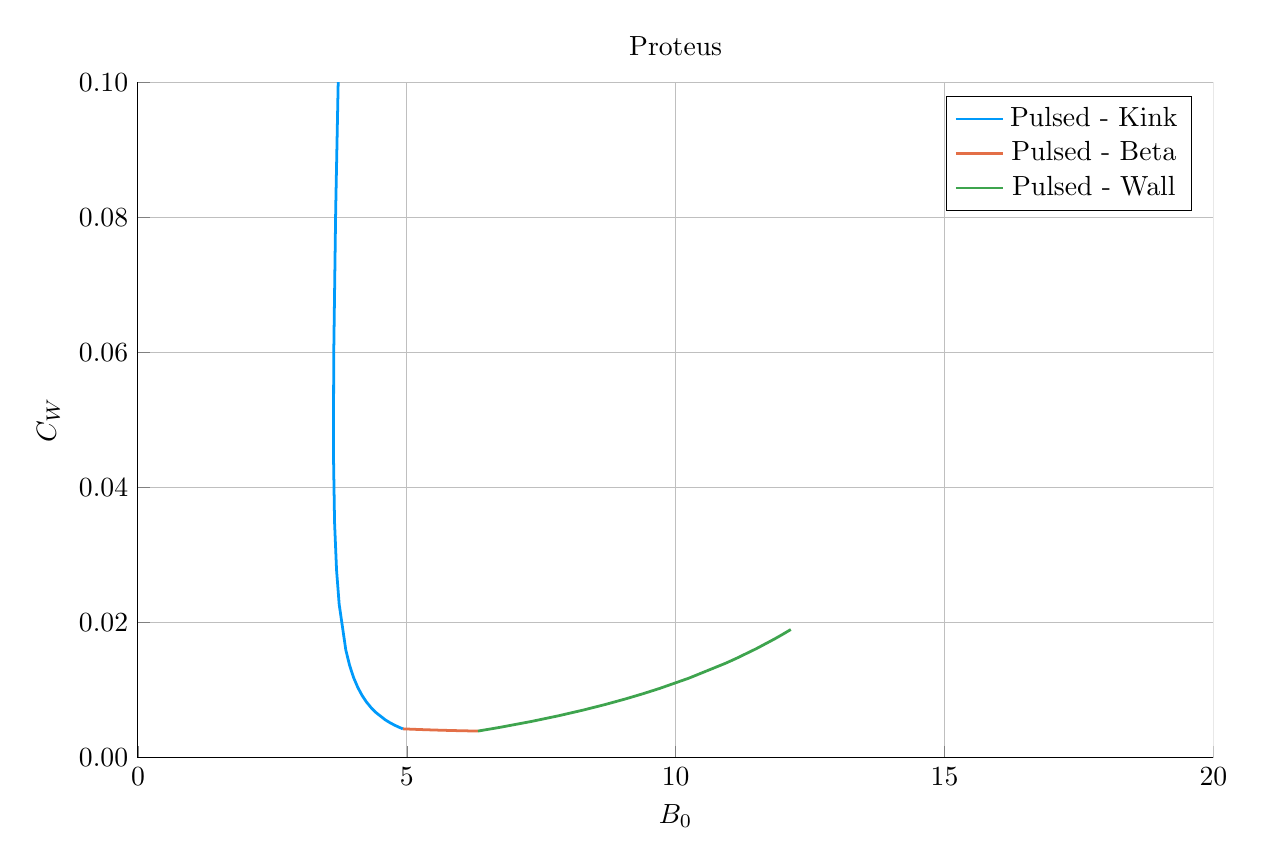
\begin{tikzpicture}[]
\begin{axis}[height = {101.6mm}, ylabel = {${C}_{W}$}, title = {Proteus}, xmin = {0.0}, xmax = {20.0}, ymax = {0.1}, xlabel = {${B}_{0}$}, {unbounded coords=jump, scaled x ticks = false, xticklabel style={rotate = 0}, xmajorgrids = true, xtick = {0.0,5.0,10.0,15.0,20.0}, xticklabels = {0,5,10,15,20}, xtick align = inside, axis lines* = left, scaled y ticks = false, yticklabel style={rotate = 0}, ymajorgrids = true, ytick = {0.0,0.02,0.04,0.06,0.08,0.1}, yticklabels = {0.00,0.02,0.04,0.06,0.08,0.10}, ytick align = inside, axis lines* = left,     xshift = 0.0mm,
    yshift = 0.0mm,
    axis background/.style={fill={rgb,1:red,1.00000000;green,1.00000000;blue,1.00000000}}
, colorbar style={title=}}, ymin = {0.0}, width = {152.4mm}]\addplot+ [color = {rgb,1:red,0.00000000;green,0.60560316;blue,0.97868012},
draw opacity=1.0,
line width=1,
solid,mark = none,
mark size = 2.0,
mark options = {
    color = {rgb,1:red,0.00000000;green,0.00000000;blue,0.00000000}, draw opacity = 1.0,
    fill = {rgb,1:red,0.00000000;green,0.60560316;blue,0.97868012}, fill opacity = 1.0,
    line width = 1,
    rotate = 0,
    solid
}]coordinates {
(4.658732060637907, 0.5238680720960677)
(4.211109766361548, 0.29158377814463826)
(3.9293920326356777, 0.17767190497429325)
(3.7651903683456465, 0.1166072358238225)
(3.6776039543745567, 0.08112372927887979)
(3.6402437753208394, 0.05909652489757084)
(3.6366994671255806, 0.04467306876996977)
(3.656621534643579, 0.03480923074663025)
(3.693300156736026, 0.02781736023114741)
(3.7422515017241134, 0.022710208007687336)
(3.865532743079537, 0.015952709019313158)
(3.936096932264377, 0.013665127664349888)
(4.010907188015084, 0.01184965388633812)
(4.089072356933184, 0.010387577045642686)
(4.169903401491354, 0.009194676609194867)
(4.252857906625248, 0.008210013517334984)
(4.337501757261618, 0.007388710643319612)
(4.42348218754058, 0.006697190814676216)
(4.5983381267510195, 0.005607443376267891)
(4.686766232902671, 0.005174363801875551)
(4.775618142770625, 0.004798727872321348)
(4.864743502376605, 0.004470996685456748)
(4.927312314219091, 0.004265648977267023)
};
\addlegendentry{Pulsed - Kink}
\addplot+ [color = {rgb,1:red,0.88887350;green,0.43564919;blue,0.27812294},
draw opacity=1.0,
line width=1,
solid,mark = none,
mark size = 2.0,
mark options = {
    color = {rgb,1:red,0.00000000;green,0.00000000;blue,0.00000000}, draw opacity = 1.0,
    fill = {rgb,1:red,0.88887350;green,0.43564919;blue,0.27812294}, fill opacity = 1.0,
    line width = 1,
    rotate = 0,
    solid
}]coordinates {
(4.927312314219091, 0.004265648977267023)
(4.984545814413324, 0.004246004028390513)
(5.17452482724068, 0.0041849470602593405)
(5.362091669637646, 0.0041306604637180565)
(5.54700293215903, 0.004082678433657853)
(5.729042482638278, 0.004040568150841258)
(5.908022832274664, 0.004003927180150204)
(6.083785777786694, 0.003972381072297988)
(6.256202341425288, 0.003945581215430235)
(6.324169421042356, 0.003936121998618512)
};
\addlegendentry{Pulsed - Beta}
\addplot+ [color = {rgb,1:red,0.24222430;green,0.64327509;blue,0.30444865},
draw opacity=1.0,
line width=1,
solid,mark = none,
mark size = 2.0,
mark options = {
    color = {rgb,1:red,0.00000000;green,0.00000000;blue,0.00000000}, draw opacity = 1.0,
    fill = {rgb,1:red,0.24222430;green,0.64327509;blue,0.30444865}, fill opacity = 1.0,
    line width = 1,
    rotate = 0,
    solid
}]coordinates {
(6.324169421042356, 0.003936121998618512)
(6.727338549778396, 0.004479602725986452)
(7.320469048424473, 0.005364564868057796)
(7.835746509376305, 0.006224935802002464)
(8.290245520072391, 0.007063234029306885)
(8.696162676727877, 0.00788223849893927)
(9.0624397222742, 0.00868451845222651)
(9.395798186463841, 0.00947231261660997)
(9.701405747258567, 0.010247527923592582)
(10.244760202900984, 0.011766415534875542)
(10.930275827723788, 0.013983337609097824)
(11.131878682735255, 0.014709436843559874)
(11.50278450645086, 0.01614615622924262)
(11.83715172742864, 0.017565397423788643)
(11.992609772603878, 0.018269423189653803)
(12.141110720831467, 0.018970135151011147)
};
\addlegendentry{Pulsed - Wall}
\end{axis}

\end{tikzpicture}

		\end{adjustbox}
        \caption{Proteus Cost-per-Watt}
    \end{subfigure}
    \hfill
    \begin{subfigure}[t]{0.45\textwidth}
        \centering
		\begin{adjustbox}{width=\textwidth}
			\Large
			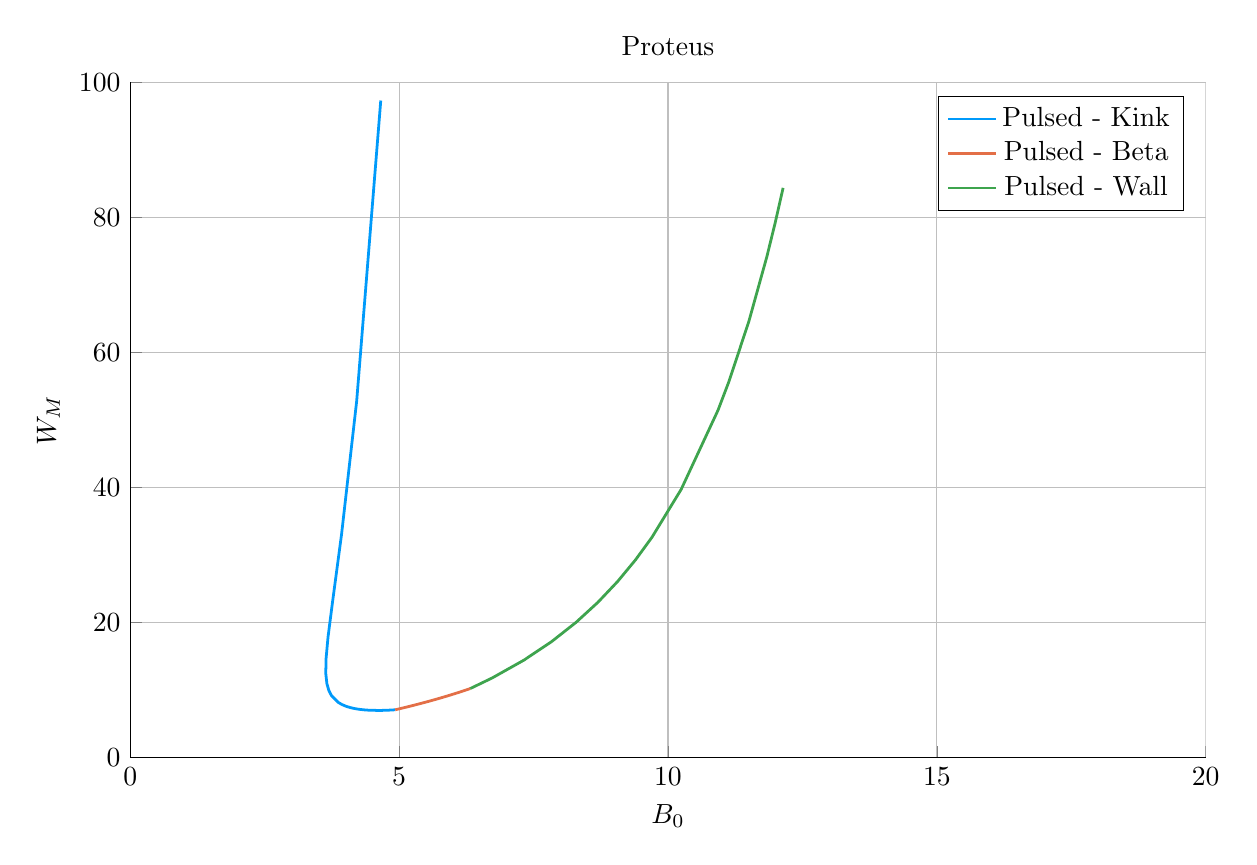
\begin{tikzpicture}[]
\begin{axis}[height = {101.6mm}, ylabel = {${W}_{M}$}, title = {Proteus}, xmin = {0.0}, xmax = {20.0}, ymax = {100.0}, xlabel = {${B}_{0}$}, {unbounded coords=jump, scaled x ticks = false, xticklabel style={rotate = 0}, xmajorgrids = true, xtick = {0.0,5.0,10.0,15.0,20.0}, xticklabels = {0,5,10,15,20}, xtick align = inside, axis lines* = left, scaled y ticks = false, yticklabel style={rotate = 0}, ymajorgrids = true, ytick = {0.0,20.0,40.0,60.0,80.0,100.0}, yticklabels = {0,20,40,60,80,100}, ytick align = inside, axis lines* = left,     xshift = 0.0mm,
    yshift = 0.0mm,
    axis background/.style={fill={rgb,1:red,1.00000000;green,1.00000000;blue,1.00000000}}
, colorbar style={title=}}, ymin = {0.0}, width = {152.4mm}]\addplot+ [color = {rgb,1:red,0.00000000;green,0.60560316;blue,0.97868012},
draw opacity=1.0,
line width=1,
solid,mark = none,
mark size = 2.0,
mark options = {
    color = {rgb,1:red,0.00000000;green,0.00000000;blue,0.00000000}, draw opacity = 1.0,
    fill = {rgb,1:red,0.00000000;green,0.60560316;blue,0.97868012}, fill opacity = 1.0,
    line width = 1,
    rotate = 0,
    solid
}]coordinates {
(4.658732060637907, 97.28232425378617)
(4.211109766361548, 52.81528522659042)
(3.9293920326356777, 33.045940900779435)
(3.7651903683456465, 23.247661382566328)
(3.6776039543745567, 17.827034690374397)
(3.6402437753208394, 14.548456710153735)
(3.6366994671255806, 12.424185075208992)
(3.656621534643579, 10.973706805818463)
(3.693300156736026, 9.943115007776825)
(3.7422515017241134, 9.18863958559583)
(3.865532743079537, 8.195040941316238)
(3.936096932264377, 7.866037710488523)
(4.010907188015084, 7.612872940496481)
(4.089072356933184, 7.418652478460303)
(4.169903401491354, 7.271257368183174)
(4.252857906625248, 7.16179941021134)
(4.337501757261618, 7.083633084260422)
(4.42348218754058, 7.031705491759868)
(4.5983381267510195, 6.991823293679325)
(4.686766232902671, 6.998413622496496)
(4.775618142770625, 7.019967223555443)
(4.864743502376605, 7.054937735216179)
(4.927312314219091, 7.086769144908002)
};
\addlegendentry{Pulsed - Kink}
\addplot+ [color = {rgb,1:red,0.88887350;green,0.43564919;blue,0.27812294},
draw opacity=1.0,
line width=1,
solid,mark = none,
mark size = 2.0,
mark options = {
    color = {rgb,1:red,0.00000000;green,0.00000000;blue,0.00000000}, draw opacity = 1.0,
    fill = {rgb,1:red,0.88887350;green,0.43564919;blue,0.27812294}, fill opacity = 1.0,
    line width = 1,
    rotate = 0,
    solid
}]coordinates {
(4.927312314219091, 7.086769144908002)
(4.984545814413324, 7.193516773221651)
(5.17452482724068, 7.558989804600146)
(5.362091669637646, 7.937858802904825)
(5.54700293215903, 8.330611438237515)
(5.729042482638278, 8.737734587814298)
(5.908022832274664, 9.159710709615348)
(6.083785777786694, 9.597014749238335)
(6.256202341425288, 10.050111620812826)
(6.324169421042356, 10.235766195929495)
};
\addlegendentry{Pulsed - Beta}
\addplot+ [color = {rgb,1:red,0.24222430;green,0.64327509;blue,0.30444865},
draw opacity=1.0,
line width=1,
solid,mark = none,
mark size = 2.0,
mark options = {
    color = {rgb,1:red,0.00000000;green,0.00000000;blue,0.00000000}, draw opacity = 1.0,
    fill = {rgb,1:red,0.24222430;green,0.64327509;blue,0.30444865}, fill opacity = 1.0,
    line width = 1,
    rotate = 0,
    solid
}]coordinates {
(6.324169421042356, 10.235766195929495)
(6.727338549778396, 11.783493156592025)
(7.320469048424473, 14.433662866898274)
(7.835746509376305, 17.179550950209588)
(8.290245520072391, 20.029490714669382)
(8.696162676727877, 22.99147222981706)
(9.0624397222742, 26.07266302814804)
(9.395798186463841, 29.27939084761122)
(9.701405747258567, 32.61725020270231)
(10.244760202900984, 39.70580850721064)
(10.930275827723788, 51.43239308745394)
(11.131878682735255, 55.64715526987581)
(11.50278450645086, 64.55415559202683)
(11.83715172742864, 74.11630708302644)
(11.992609772603878, 79.14953842129572)
(12.141110720831467, 84.35411724014395)
};
\addlegendentry{Pulsed - Wall}
\end{axis}

\end{tikzpicture}

		\end{adjustbox}
        \caption{Proteus Capital Cost}
    \end{subfigure}
    \hfill \hfill ~\\ ~\\ ~\\ ~\\
    \hfill
    \begin{subfigure}[t]{0.45\textwidth}
        \centering
		\begin{adjustbox}{width=\textwidth}
			\Large
			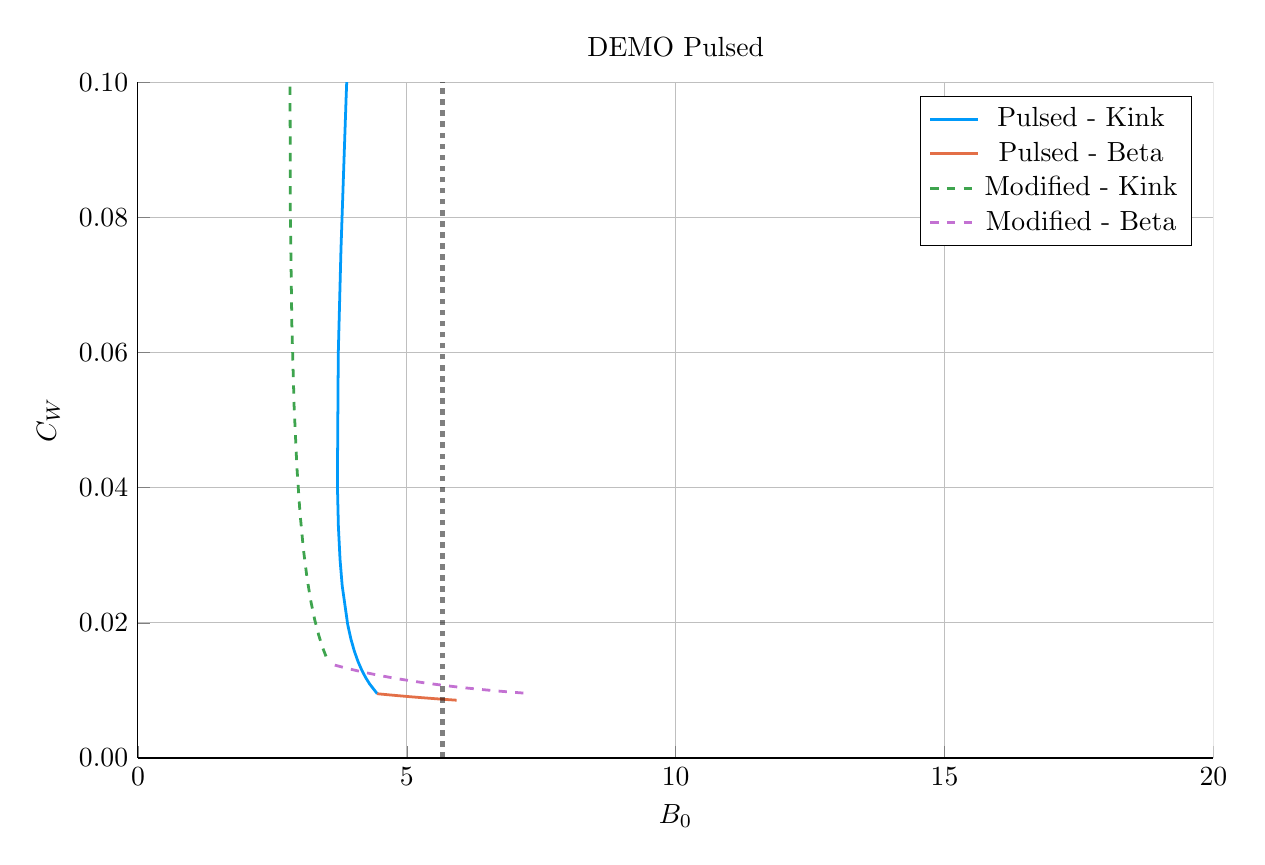
\begin{tikzpicture}[]
\begin{axis}[height = {101.6mm}, ylabel = {${C}_{W}$}, title = {DEMO Pulsed}, xmin = {0.0}, xmax = {20.0}, ymax = {0.1}, xlabel = {${B}_{0}$}, {unbounded coords=jump, scaled x ticks = false, xticklabel style={rotate = 0}, xmajorgrids = true, xtick = {0.0,5.0,10.0,15.0,20.0}, xticklabels = {0,5,10,15,20}, xtick align = inside, axis lines* = left, scaled y ticks = false, yticklabel style={rotate = 0}, ymajorgrids = true, ytick = {0.0,0.02,0.04,0.06,0.08,0.1}, yticklabels = {0.00,0.02,0.04,0.06,0.08,0.10}, ytick align = inside, axis lines* = left,     xshift = 0.0mm,
    yshift = 0.0mm,
    axis background/.style={fill={rgb,1:red,1.00000000;green,1.00000000;blue,1.00000000}}
, colorbar style={title=}}, ymin = {0.0}, width = {152.4mm}]\addplot+ [color = {rgb,1:red,0.00000000;green,0.60560316;blue,0.97868012},
draw opacity=1.0,
line width=1,
solid,mark = none,
mark size = 2.0,
mark options = {
    color = {rgb,1:red,0.00000000;green,0.00000000;blue,0.00000000}, draw opacity = 1.0,
    fill = {rgb,1:red,0.00000000;green,0.60560316;blue,0.97868012}, fill opacity = 1.0,
    line width = 1,
    rotate = 0,
    solid
}]coordinates {
(4.327031075670194, 0.1892287825513326)
(4.038214026054326, 0.13206162052102163)
(3.8713719163129245, 0.09770836377510679)
(3.7758613845615545, 0.0753228145367537)
(3.7257856761317214, 0.05989044017674145)
(3.7090473695925437, 0.04055229837333577)
(3.727711597554826, 0.03426367140819575)
(3.7586131667481433, 0.029359319233913946)
(3.799052518631718, 0.025462690957960717)
(3.901290136389271, 0.019741499311841708)
(3.960577465316514, 0.017607284508542168)
(4.0241209645210345, 0.015819330878112364)
(4.0912717805663785, 0.014306863958145555)
(4.161514602943343, 0.013016229386127556)
(4.2344343960723005, 0.0119061698584303)
(4.309692554546368, 0.010944552619225426)
(4.450417240491067, 0.009508186007059894)
};
\addlegendentry{Pulsed - Kink}
\addplot+ [color = {rgb,1:red,0.88887350;green,0.43564919;blue,0.27812294},
draw opacity=1.0,
line width=1,
solid,mark = none,
mark size = 2.0,
mark options = {
    color = {rgb,1:red,0.00000000;green,0.00000000;blue,0.00000000}, draw opacity = 1.0,
    fill = {rgb,1:red,0.88887350;green,0.43564919;blue,0.27812294}, fill opacity = 1.0,
    line width = 1,
    rotate = 0,
    solid
}]coordinates {
(4.450417240491067, 0.009508186007059894)
(4.490148631384312, 0.009477474217304566)
(4.692490181445514, 0.009325449924582748)
(4.8960344619053355, 0.009179881556836224)
(5.100651132702229, 0.00904086745514222)
(5.306202822090688, 0.008908420253381469)
(5.512545696627038, 0.008782491226353)
(5.719530043226767, 0.008662988371093566)
(5.927000883375481, 0.00854978980550123)
};
\addlegendentry{Pulsed - Beta}
\addplot+ [color = {rgb,1:red,0.24222430;green,0.64327509;blue,0.30444865},
draw opacity=1.0,
line width=1,
dashed,mark = none,
mark size = 2.0,
mark options = {
    color = {rgb,1:red,0.00000000;green,0.00000000;blue,0.00000000}, draw opacity = 1.0,
    fill = {rgb,1:red,0.24222430;green,0.64327509;blue,0.30444865}, fill opacity = 1.0,
    line width = 1,
    rotate = 0,
    solid
}]coordinates {
(3.4087424183072135, 0.34025279914240075)
(2.977074181068944, 0.20266043375242454)
(2.8592500074202523, 0.14107963570535767)
(2.827199220063259, 0.10460917631328934)
(2.8339789008667826, 0.08069963800921795)
(2.862412302880871, 0.06408640910554732)
(2.9044598258085443, 0.05207050885933721)
(2.95577893007882, 0.04311069749575431)
(3.0137895352525907, 0.03626387631819784)
(3.076849710218805, 0.03092374739004359)
(3.1438583711612704, 0.02668548743841045)
(3.214045733980633, 0.023270423882766844)
(3.2868548955983727, 0.020481784288090023)
(3.361871149981842, 0.018177576354657807)
(3.4387778750377818, 0.016253383634250513)
(3.5173279629378453, 0.014631131503744007)
};
\addlegendentry{Modified - Kink}
\addplot+ [color = {rgb,1:red,0.76444018;green,0.44411178;blue,0.82429754},
draw opacity=1.0,
line width=1,
dashed,mark = none,
mark size = 2.0,
mark options = {
    color = {rgb,1:red,0.00000000;green,0.00000000;blue,0.00000000}, draw opacity = 1.0,
    fill = {rgb,1:red,0.76444018;green,0.44411178;blue,0.82429754}, fill opacity = 1.0,
    line width = 1,
    rotate = 0,
    solid
}]coordinates {
(3.6607028750648505, 0.013744899135556416)
(3.8574448036470477, 0.013332033203155177)
(4.056375867871351, 0.012949491171136135)
(4.257366397480293, 0.012594759179481692)
(4.460279103534801, 0.012265542491796714)
(4.664969389370631, 0.011959760748489753)
(4.871285596007394, 0.011675536110154509)
(5.07906923307514, 0.01141117796484883)
(5.288155233306219, 0.011165166374807946)
(5.498372259673351, 0.010936135522073528)
(5.709543087166185, 0.010722857854384784)
(5.921485076209294, 0.010524229289897682)
(6.134010749367255, 0.010339255636975386)
(6.346928478632384, 0.0101670402635639)
(6.560043285872518, 0.010006772983002756)
(6.773157754368795, 0.009857720087022352)
(6.986073044284746, 0.009719215441404045)
(7.198590001107076, 0.00959065255201969)
};
\addlegendentry{Modified - Beta}
\addplot+ [color = {rgb,1:red,0.00000000;green,0.00000000;blue,0.00000000},
draw opacity=0.5,
line width=2,
dotted,mark = none,
mark size = 2.0,
mark options = {
    color = {rgb,1:red,0.00000000;green,0.00000000;blue,0.00000000}, draw opacity = 0.5,
    fill = {rgb,1:red,0.00000000;green,0.00000000;blue,0.00000000}, fill opacity = 0.5,
    line width = 1,
    rotate = 0,
    solid
},forget plot]coordinates {
(0.0, NaN)
(20.0, NaN)
};
\addplot+ [color = {rgb,1:red,0.00000000;green,0.00000000;blue,0.00000000},
draw opacity=0.5,
line width=2,
dotted,mark = none,
mark size = 2.0,
mark options = {
    color = {rgb,1:red,0.00000000;green,0.00000000;blue,0.00000000}, draw opacity = 0.5,
    fill = {rgb,1:red,0.00000000;green,0.00000000;blue,0.00000000}, fill opacity = 0.5,
    line width = 1,
    rotate = 0,
    solid
},forget plot]coordinates {
(5.667, 0.0)
(5.667, 0.1)
};
\addplot+[draw=none, color = {rgb,1:red,0.00000000;green,0.00000000;blue,0.00000000},
draw opacity=0.5,
line width=0,
solid,mark = *,
mark size = 2.0,
mark options = {
    color = {rgb,1:red,0.00000000;green,0.00000000;blue,0.00000000}, draw opacity = 0.5,
    fill = {rgb,1:red,0.00000000;green,0.00000000;blue,0.00000000}, fill opacity = 0.5,
    line width = 1,
    rotate = 0,
    solid
},forget plot] coordinates {
(5.667, NaN)
};
\end{axis}

\end{tikzpicture}

		\end{adjustbox}
        \caption{DEMO Pulsed Cost-per-Watt}
    \end{subfigure}
    \hfill
    \begin{subfigure}[t]{0.45\textwidth}
        \centering
		\begin{adjustbox}{width=\textwidth}
			\Large
			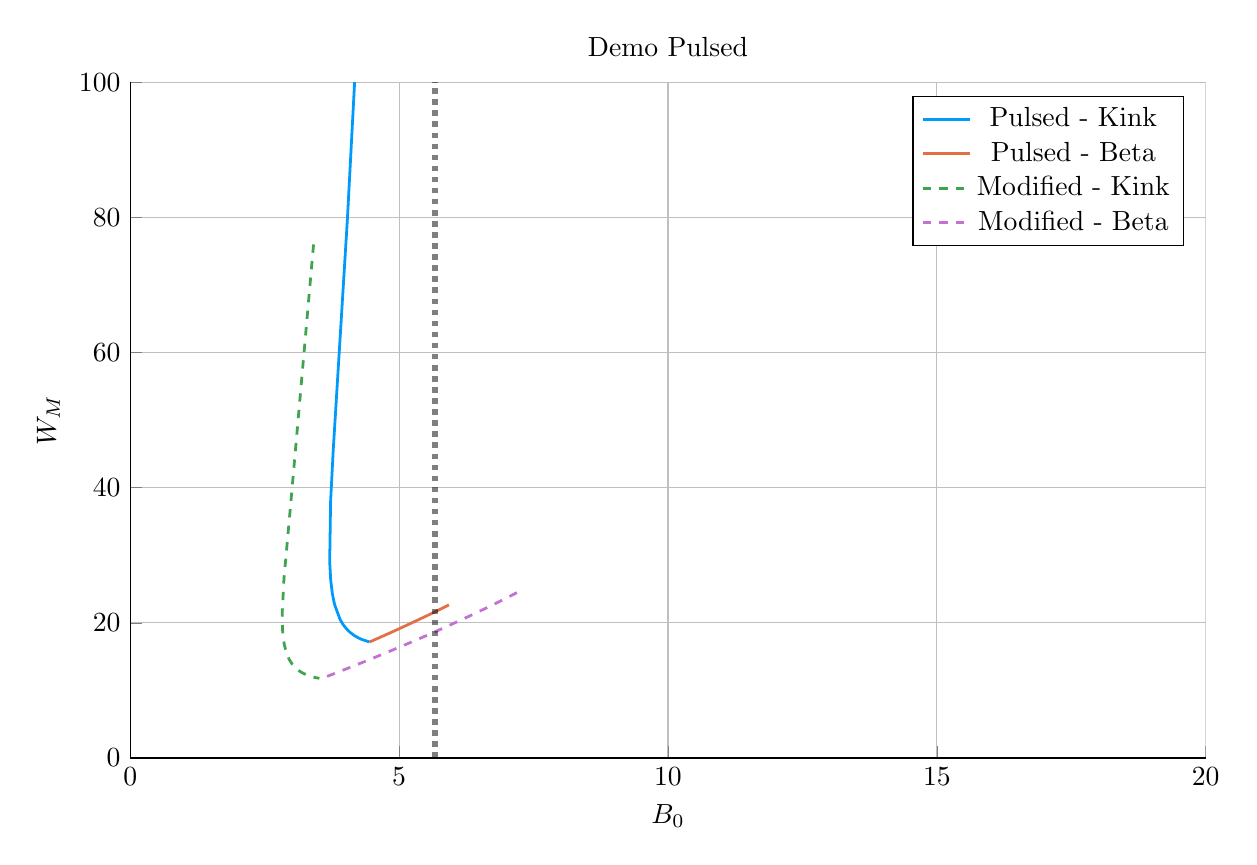
\begin{tikzpicture}[]
\begin{axis}[height = {101.6mm}, ylabel = {${W}_{M}$}, title = {Demo Pulsed}, xmin = {0.0}, xmax = {20.0}, ymax = {100.0}, xlabel = {${B}_{0}$}, {unbounded coords=jump, scaled x ticks = false, xticklabel style={rotate = 0}, xmajorgrids = true, xtick = {0.0,5.0,10.0,15.0,20.0}, xticklabels = {0,5,10,15,20}, xtick align = inside, axis lines* = left, scaled y ticks = false, yticklabel style={rotate = 0}, ymajorgrids = true, ytick = {0.0,20.0,40.0,60.0,80.0,100.0}, yticklabels = {0,20,40,60,80,100}, ytick align = inside, axis lines* = left,     xshift = 0.0mm,
    yshift = 0.0mm,
    axis background/.style={fill={rgb,1:red,1.00000000;green,1.00000000;blue,1.00000000}}
, colorbar style={title=}}, ymin = {0.0}, width = {152.4mm}]\addplot+ [color = {rgb,1:red,0.00000000;green,0.60560316;blue,0.97868012},
draw opacity=1.0,
line width=1,
solid,mark = none,
mark size = 2.0,
mark options = {
    color = {rgb,1:red,0.00000000;green,0.00000000;blue,0.00000000}, draw opacity = 1.0,
    fill = {rgb,1:red,0.00000000;green,0.60560316;blue,0.97868012}, fill opacity = 1.0,
    line width = 1,
    rotate = 0,
    solid
}]coordinates {
(4.327031075670194, 123.44373673332173)
(4.038214026054326, 79.76523284023226)
(3.8713719163129245, 58.108897430981536)
(3.7758613845615545, 45.733304605517155)
(3.7257856761317214, 37.95828264093558)
(3.7090473695925437, 29.04694896379975)
(3.727711597554826, 26.344517979953586)
(3.7586131667481433, 24.306117941226923)
(3.799052518631718, 22.733747168495924)
(3.901290136389271, 20.517766605492294)
(3.960577465316514, 19.728940193613518)
(4.0241209645210345, 19.090733790490855)
(4.0912717805663785, 18.572256162198553)
(4.161514602943343, 18.150497380470465)
(4.2344343960723005, 17.808002600991745)
(4.309692554546368, 17.531315861496644)
(4.450417240491067, 17.166473566094577)
};
\addlegendentry{Pulsed - Kink}
\addplot+ [color = {rgb,1:red,0.88887350;green,0.43564919;blue,0.27812294},
draw opacity=1.0,
line width=1,
solid,mark = none,
mark size = 2.0,
mark options = {
    color = {rgb,1:red,0.00000000;green,0.00000000;blue,0.00000000}, draw opacity = 1.0,
    fill = {rgb,1:red,0.88887350;green,0.43564919;blue,0.27812294}, fill opacity = 1.0,
    line width = 1,
    rotate = 0,
    solid
}]coordinates {
(4.450417240491067, 17.166473566094577)
(4.490148631384312, 17.305309015848636)
(4.692490181445514, 18.019389484737392)
(4.8960344619053355, 18.749800407200777)
(5.100651132702229, 19.496700146051747)
(5.306202822090688, 20.26030213940914)
(5.512545696627038, 21.04087102241869)
(5.719530043226767, 21.83871936060431)
(5.927000883375481, 22.654204785704835)
};
\addlegendentry{Pulsed - Beta}
\addplot+ [color = {rgb,1:red,0.24222430;green,0.64327509;blue,0.30444865},
draw opacity=1.0,
line width=1,
dashed,mark = none,
mark size = 2.0,
mark options = {
    color = {rgb,1:red,0.00000000;green,0.00000000;blue,0.00000000}, draw opacity = 1.0,
    fill = {rgb,1:red,0.24222430;green,0.64327509;blue,0.30444865}, fill opacity = 1.0,
    line width = 1,
    rotate = 0,
    solid
}]coordinates {
(3.4087424183072135, 76.02109466923234)
(2.977074181068944, 36.99469776498375)
(2.8592500074202523, 26.602664601337402)
(2.827199220063259, 21.660862067495565)
(2.8339789008667826, 18.765953821795108)
(2.862412302880871, 16.874407011263102)
(2.9044598258085443, 15.553537101768894)
(2.95577893007882, 14.590024878457532)
(3.0137895352525907, 13.865991589551562)
(3.076849710218805, 13.310773511983673)
(3.1438583711612704, 12.879335564625128)
(3.214045733980633, 12.54157019826116)
(3.2868548955983727, 12.276561049231674)
(3.361871149981842, 12.069311294803374)
(3.4387778750377818, 11.90878112839417)
(3.5173279629378453, 11.786660090388734)
};
\addlegendentry{Modified - Kink}
\addplot+ [color = {rgb,1:red,0.76444018;green,0.44411178;blue,0.82429754},
draw opacity=1.0,
line width=1,
dashed,mark = none,
mark size = 2.0,
mark options = {
    color = {rgb,1:red,0.00000000;green,0.00000000;blue,0.00000000}, draw opacity = 1.0,
    fill = {rgb,1:red,0.76444018;green,0.44411178;blue,0.82429754}, fill opacity = 1.0,
    line width = 1,
    rotate = 0,
    solid
}]coordinates {
(3.6607028750648505, 12.074397140834275)
(3.8574448036470477, 12.685277919648211)
(4.056375867871351, 13.310146449544076)
(4.257366397480293, 13.949057026240864)
(4.460279103534801, 14.602113733589642)
(4.664969389370631, 15.269467629207359)
(4.871285596007394, 15.951314711845848)
(5.07906923307514, 16.647894398080105)
(5.288155233306219, 17.359488308762714)
(5.498372259673351, 18.086419214151615)
(5.709543087166185, 18.82905002156669)
(5.921485076209294, 19.587782712469505)
(6.134010749367255, 20.363057156601585)
(6.346928478632384, 21.155349745799302)
(6.560043285872518, 21.965171804607706)
(6.773157754368795, 22.79306774804729)
(6.986073044284746, 23.639612971086876)
(7.198590001107076, 24.50541146426436)
};
\addlegendentry{Modified - Beta}
\addplot+ [color = {rgb,1:red,0.00000000;green,0.00000000;blue,0.00000000},
draw opacity=0.5,
line width=2,
dotted,mark = none,
mark size = 2.0,
mark options = {
    color = {rgb,1:red,0.00000000;green,0.00000000;blue,0.00000000}, draw opacity = 0.5,
    fill = {rgb,1:red,0.00000000;green,0.00000000;blue,0.00000000}, fill opacity = 0.5,
    line width = 1,
    rotate = 0,
    solid
},forget plot]coordinates {
(0.0, NaN)
(20.0, NaN)
};
\addplot+ [color = {rgb,1:red,0.00000000;green,0.00000000;blue,0.00000000},
draw opacity=0.5,
line width=2,
dotted,mark = none,
mark size = 2.0,
mark options = {
    color = {rgb,1:red,0.00000000;green,0.00000000;blue,0.00000000}, draw opacity = 0.5,
    fill = {rgb,1:red,0.00000000;green,0.00000000;blue,0.00000000}, fill opacity = 0.5,
    line width = 1,
    rotate = 0,
    solid
},forget plot]coordinates {
(5.667, 0.0)
(5.667, 100.0)
};
\addplot+[draw=none, color = {rgb,1:red,0.00000000;green,0.00000000;blue,0.00000000},
draw opacity=0.5,
line width=0,
solid,mark = *,
mark size = 2.0,
mark options = {
    color = {rgb,1:red,0.00000000;green,0.00000000;blue,0.00000000}, draw opacity = 0.5,
    fill = {rgb,1:red,0.00000000;green,0.00000000;blue,0.00000000}, fill opacity = 0.5,
    line width = 1,
    rotate = 0,
    solid
},forget plot] coordinates {
(5.667, NaN)
};
\end{axis}

\end{tikzpicture}

		\end{adjustbox}
        \caption{DEMO Pulsed Capital Cost}
    \end{subfigure}
    \hfill \hfill ~\\ ~\\ ~\\
    \caption{Pulsed Cost Curves}
    \label{fig:pulsed_costs} ~ \\
    \added{\small Pulsed reactor design is slightly more ambiguous than steady-state in terms of selecting an operating point. These plots show that the cost-per-watt is reduced at the highest field strength available to \texttt{beta} regime reactors. The minimum capital cost then occurs when the \texttt{beta} and \texttt{kink} limit are both just marginally satisfied. }
\end{figure*}

\clearpage

\newpage

\subsection{Utilizing High Field Magnets}

\label{subsection:high_field}

The main conclusion for this paper is that high field magnets are the way to go to build an \replaced{economic}{efficient}, compact fusion reactor. In line with the MIT ARC effort, these high fields will be built with high-temperature superconducting (HTS) tape. This innovation is set to \added{nearly} double the strength of conventional magnets. The real question is how best to use this technology.

At a very simple level, there are two main places strong magnets can be employed: the toroidal fields ($B_0$) and the central solenoid ($B_{CS}$). The easier mode of operation to start with is steady-state. This is because steady-state tokamaks do not rely on a central solenoid \replaced{to run their functionally infinite length pulses.}{for the profitability of their machines.} Further, the cost curves in \cref{fig:steady_cost} show that all these designs would benefit from toroidal fields ($B_0$) not achievable with conventional magnets -- which can only reach around \replaced{13 T.\cite{hartmann}}{10 T on a good day.}

The more interesting result is that pulsed reactors gain no real benefit from using HTS toroidal field magnets \added{-- as mentioned previously in \cref{subsection:operation_differences}}. Within the modern paradigm (i.e.\ D-T fuel, H-Mode, etc), pulsed reactors never have to exceed the limits of \replaced{less expensive LTS magnets.}{inexpensive, copper magnets.} The place HTS can really help is with the central solenoid, which governs how long a pulse can last. Further, \replaced{improvements to}{the effect of improving} the central solenoid \replaced{have diminishing returns past}{saturates within} the range accessible to HTS tape. Again, HTS would be more than adequate for the modern paradigm. These conclusions are shown in \cref{fig:pulsed_sensitivities,fig:pulsed_samplings}.

\begin{figure*}
    \centering
    \hfill
    \begin{subfigure}[t]{0.45\textwidth}
        \centering
    \begin{adjustbox}{width=\textwidth}
      \Large
      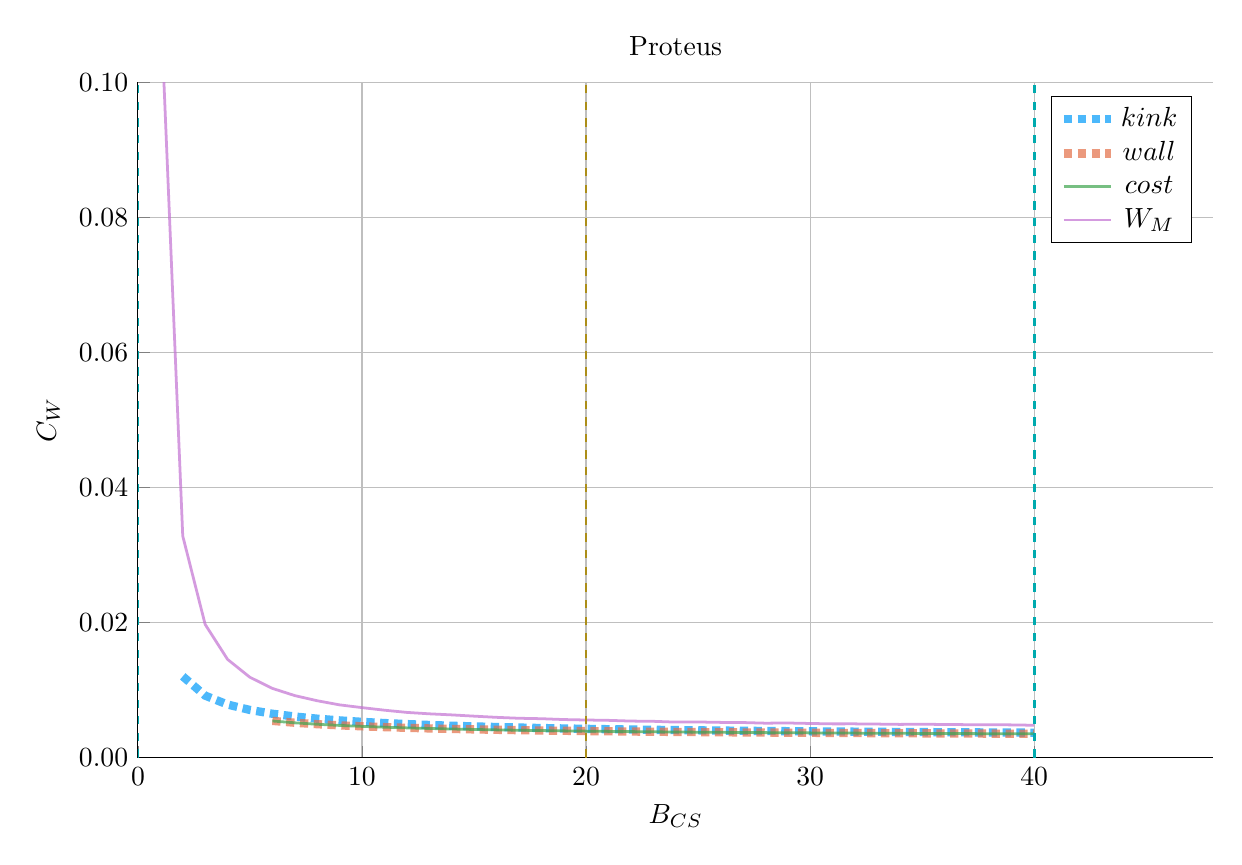
\begin{tikzpicture}[]
\begin{axis}[height = {101.6mm}, ylabel = {${C}_{W}$}, title = {Proteus}, xmin = {0.0}, xmax = {48.0}, ymax = {0.1}, xlabel = {${B}_{CS}$}, {unbounded coords=jump, scaled x ticks = false, xticklabel style={rotate = 0}, xmajorgrids = true, xtick = {0.0,10.0,20.0,30.0,40.0}, xticklabels = {0,10,20,30,40}, xtick align = inside, axis lines* = left, scaled y ticks = false, yticklabel style={rotate = 0}, ymajorgrids = true, ytick = {0.0,0.02,0.04,0.06,0.08,0.1}, yticklabels = {0.00,0.02,0.04,0.06,0.08,0.10}, ytick align = inside, axis lines* = left,     xshift = 0.0mm,
    yshift = 0.0mm,
    axis background/.style={fill={rgb,1:red,1.00000000;green,1.00000000;blue,1.00000000}}
, colorbar style={title=}}, ymin = {0.0}, width = {152.4mm}]\addplot+ [color = {rgb,1:red,0.00000000;green,0.60560316;blue,0.97868012},
draw opacity=0.7,
line width=3,
dotted,mark = none,
mark size = 2.0,
mark options = {
    color = {rgb,1:red,0.00000000;green,0.00000000;blue,0.00000000}, draw opacity = 0.7,
    fill = {rgb,1:red,0.00000000;green,0.60560316;blue,0.97868012}, fill opacity = 0.7,
    line width = 1,
    rotate = 0,
    solid
}]coordinates {
(2.0, 0.01203588028473762)
(3.0, 0.009184398565447248)
(4.0, 0.007862884013421416)
(5.0, 0.007057989599185806)
(6.0, 0.006502613319842857)
(7.0, 0.006090672614199328)
(8.0, 0.005770350019203115)
(9.0, 0.005512859892710094)
(10.0, 0.005300727695239639)
(11.0, 0.005122630604633569)
(12.0, 0.004970854616305319)
(13.0, 0.00483993073972795)
(14.0, 0.0047258536533321)
(15.0, 0.004625609812173743)
(16.0, 0.004536878856245803)
(17.0, 0.004457840030041975)
(18.0, 0.004387039347241793)
(19.0, 0.004323297793305687)
(20.0, 0.004265648725148842)
(21.0, 0.00421328852908289)
(22.0, 0.004165543387382086)
(23.0, 0.0041218418382133306)
(24.0, 0.004081697424729452)
(25.0, 0.004044691025187507)
(26.0, 0.004010460170934446)
(27.0, 0.00397868942182741)
(28.0, 0.003949102890414613)
(29.0, 0.003921458228696752)
(30.0, 0.0038955417483358588)
(31.0, 0.00387116442730114)
(32.0, 0.003848158715413871)
(33.0, 0.0038263753834889853)
(34.0, 0.003805681791784416)
(35.0, 0.0037859598267780737)
(36.0, 0.003767103936991627)
(37.0, 0.003749019788626583)
(38.0, 0.0037316235037579658)
(39.0, 0.0037148400629903496)
(40.0, 0.003698602652227772)
};
\addlegendentry{$kink$}
\addplot+ [color = {rgb,1:red,0.88887350;green,0.43564919;blue,0.27812294},
draw opacity=0.7,
line width=3,
dotted,mark = none,
mark size = 2.0,
mark options = {
    color = {rgb,1:red,0.00000000;green,0.00000000;blue,0.00000000}, draw opacity = 0.7,
    fill = {rgb,1:red,0.88887350;green,0.43564919;blue,0.27812294}, fill opacity = 0.7,
    line width = 1,
    rotate = 0,
    solid
}]coordinates {
(6.0, 0.0054444534313977866)
(7.0, 0.005168634641274746)
(8.0, 0.004954271193511655)
(9.0, 0.004781774855931542)
(10.0, 0.0046393940524333595)
(11.0, 0.004519572327657892)
(12.0, 0.004417187891782309)
(13.0, 0.004328621916738755)
(14.0, 0.004251229863078844)
(15.0, 0.004183024392188461)
(16.0, 0.004122476375660697)
(17.0, 0.004068385219748399)
(18.0, 0.004019791621043741)
(19.0, 0.003975917241919141)
(20.0, 0.003936121998618529)
(21.0, 0.0038998731854890116)
(22.0, 0.0038667227426346573)
(23.0, 0.0038362902440819057)
(24.0, 0.003808249979473852)
(25.0, 0.003782321013899768)
(26.0, 0.003758259446775421)
(27.0, 0.003735852316365348)
(28.0, 0.0037149127505960292)
(29.0, 0.0036952760721994664)
(30.0, 0.003676796641638663)
(31.0, 0.003659345275564596)
(32.0, 0.003642807117806076)
(33.0, 0.0036270798687725717)
(34.0, 0.003612072300608303)
(35.0, 0.0035977030015636596)
(36.0, 0.0035838993052924165)
(37.0, 0.003570596370170802)
(38.0, 0.0035577363809944163)
(39.0, 0.003545267851071995)
(40.0, 0.003533145007184075)
};
\addlegendentry{$wall$}
\addplot+ [color = {rgb,1:red,0.24222430;green,0.64327509;blue,0.30444865},
draw opacity=0.7,
line width=1,
solid,mark = none,
mark size = 2.0,
mark options = {
    color = {rgb,1:red,0.00000000;green,0.00000000;blue,0.00000000}, draw opacity = 0.7,
    fill = {rgb,1:red,0.24222430;green,0.64327509;blue,0.30444865}, fill opacity = 0.7,
    line width = 1,
    rotate = 0,
    solid
}]coordinates {
(6.0, 0.005431918985170686) 
(7.0, 0.005156651927896806)
(8.0, 0.0049427222925668)
(9.0, 0.004770577307210836)
(10.0, 0.004628487505103093)
(11.0, 0.004508911021409933)
(12.0, 0.004406736153465557)
(13.0, 0.004318351239259131)
(14.0, 0.0042411171388798095)
(15.0, 0.004173050519899446)
(16.0, 0.00411262543808849)
(17.0, 0.0040586437812760905)
(18.0, 0.004010148222137883)
(19.0, 0.003966362101140297)
(20.0, 0.003926646631736614)
(21.0, 0.003890470261769361)
(22.0, 0.003857385855340664)
(23.0, 0.003827013846123357)
(24.0, 0.003799029152446192)
(25.0, 0.0037731515135378028)
(26.0, 0.0037491374742800476)
(27.0, 0.003726774572373303)
(28.0, 0.0037058763309042774)
(29.0, 0.0036862784148944654)
(30.0, 0.0036678355176402353)
(31.0, 0.0036504187072176437)
(32.0, 0.0036339133609214515)
(33.0, 0.003618217419267161)
(34.0, 0.003603239855200063)
(35.0, 0.0035888993956205303)
(36.0, 0.003575123536625824)
(37.0, 0.0035618476053302967)
(38.0, 0.00354901385682175)
(39.0, 0.0035365709088021192)
(40.0, 0.0035244731223137145)
};
\addlegendentry{$cost$}
\addplot+ [color = {rgb,1:red,0.76444018;green,0.44411178;blue,0.82429754},
draw opacity=0.7,
line width=1,
solid,mark = none,
mark size = 2.0,
mark options = {
    color = {rgb,1:red,0.00000000;green,0.00000000;blue,0.00000000}, draw opacity = 0.7,
    fill = {rgb,1:red,0.76444018;green,0.44411178;blue,0.82429754}, fill opacity = 0.7,
    line width = 1,
    rotate = 0,
    solid
}]coordinates {
(1.0, 0.11281791824873516)
(2.0, 0.032817502153924004)
(3.0, 0.019728226993225767)
(4.0, 0.014550673387607675)
(5.0, 0.01189537503222638)
(6.0, 0.010254586386818185)
(7.0, 0.009187722848027494)
(8.0, 0.008426409595366063)
(9.0, 0.007814460956383539)
(10.0, 0.007407116893402244)
(11.0, 0.007026609234473925)
(12.0, 0.006699623094822548)
(13.0, 0.006490049586328449)
(14.0, 0.006332285776340749)
(15.0, 0.006145121123500574)
(16.0, 0.005968637732544897)
(17.0, 0.005831116183284295)
(18.0, 0.005766436928694199)
(19.0, 0.005641758652539625)
(20.0, 0.005573536740322697)
(21.0, 0.005522757977005573)
(22.0, 0.005416005772196298)
(23.0, 0.005379655600977924)
(24.0, 0.005261536268439173)
(25.0, 0.005281022329992938)
(26.0, 0.0052218684208626695)
(27.0, 0.005199327855049588)
(28.0, 0.005104248642193906)
(29.0, 0.005130959429711627)
(30.0, 0.005061392939220031)
(31.0, 0.005001395595923804)
(32.0, 0.005003038146366862)
(33.0, 0.004969709625977857)
(34.0, 0.004924506782614121)
(35.0, 0.004946663939864212)
(36.0, 0.004912455965902953)
(37.0, 0.004883749116586274)
(38.0, 0.004871307710986148)
(39.0, 0.004851151446945242)
(40.0, 0.004795575554984452)
};
\addlegendentry{$W_M$}
\addplot+ [color = {rgb,1:red,0.67554396;green,0.55566233;blue,0.09423434},
draw opacity=1.0,
line width=1,
dashed,mark = none,
mark size = 2.0,
mark options = {
    color = {rgb,1:red,0.00000000;green,0.00000000;blue,0.00000000}, draw opacity = 1.0,
    fill = {rgb,1:red,0.67554396;green,0.55566233;blue,0.09423434}, fill opacity = 1.0,
    line width = 1,
    rotate = 0,
    solid
},forget plot]coordinates {
(20.0, 0.0)
(20.0, 0.1)
};
\addplot+ [color = {rgb,1:red,0.00000048;green,0.66575898;blue,0.68099695},
draw opacity=1.0,
line width=1,
dashed,mark = none,
mark size = 2.0,
mark options = {
    color = {rgb,1:red,0.00000000;green,0.00000000;blue,0.00000000}, draw opacity = 1.0,
    fill = {rgb,1:red,0.00000048;green,0.66575898;blue,0.68099695}, fill opacity = 1.0,
    line width = 1,
    rotate = 0,
    solid
},forget plot]coordinates {
(0.0, 0.0)
(0.0, 0.1)
};
\addplot+ [color = {rgb,1:red,0.00000048;green,0.66575898;blue,0.68099695},
draw opacity=1.0,
line width=1,
dashed,mark = none,
mark size = 2.0,
mark options = {
    color = {rgb,1:red,0.00000000;green,0.00000000;blue,0.00000000}, draw opacity = 1.0,
    fill = {rgb,1:red,0.00000048;green,0.66575898;blue,0.68099695}, fill opacity = 1.0,
    line width = 1,
    rotate = 0,
    solid
},forget plot]coordinates {
(40.0, 0.0)
(40.0, 0.1)
};
\end{axis}

\end{tikzpicture}

    \end{adjustbox}
        \caption{Proteus Cost-per-Watt}
    \end{subfigure}
    \hfill
    \begin{subfigure}[t]{0.45\textwidth}
        \centering
    \begin{adjustbox}{width=\textwidth}
      \Large
      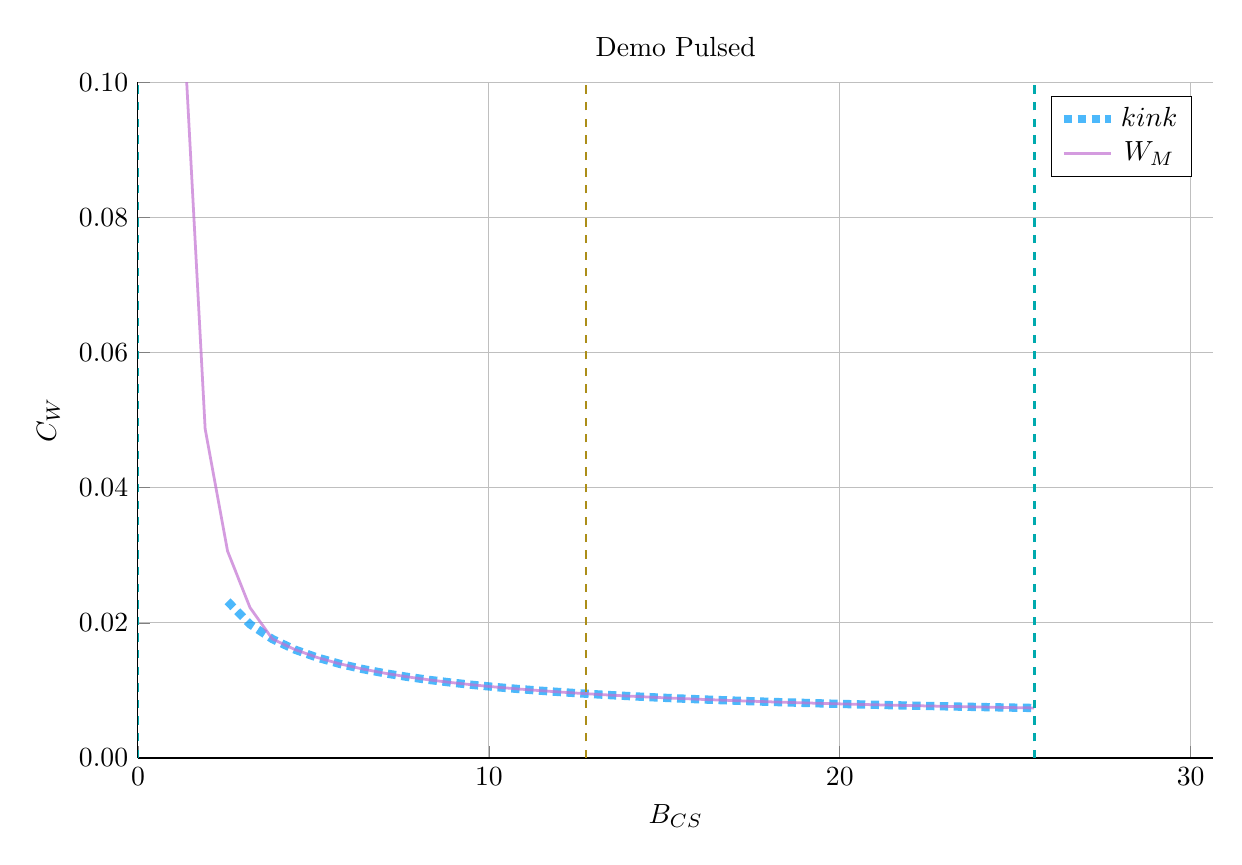
\begin{tikzpicture}[]
\begin{axis}[height = {101.6mm}, ylabel = {${C}_{W}$}, title = {Demo Pulsed}, xmin = {0.0}, xmax = {30.647999999999996}, ymax = {0.1}, xlabel = {${B}_{CS}$}, {unbounded coords=jump, scaled x ticks = false, xticklabel style={rotate = 0}, xmajorgrids = true, xtick = {0.0,10.0,20.0,30.0}, xticklabels = {0,10,20,30}, xtick align = inside, axis lines* = left, scaled y ticks = false, yticklabel style={rotate = 0}, ymajorgrids = true, ytick = {0.0,0.02,0.04,0.06,0.08,0.1}, yticklabels = {0.00,0.02,0.04,0.06,0.08,0.10}, ytick align = inside, axis lines* = left,     xshift = 0.0mm,
    yshift = 0.0mm,
    axis background/.style={fill={rgb,1:red,1.00000000;green,1.00000000;blue,1.00000000}}
, colorbar style={title=}}, ymin = {0.0}, width = {152.4mm}]\addplot+ [color = {rgb,1:red,0.00000000;green,0.60560316;blue,0.97868012},
draw opacity=0.7,
line width=3,
dotted,mark = none,
mark size = 2.0,
mark options = {
    color = {rgb,1:red,0.00000000;green,0.00000000;blue,0.00000000}, draw opacity = 0.7,
    fill = {rgb,1:red,0.00000000;green,0.60560316;blue,0.97868012}, fill opacity = 0.7,
    line width = 1,
    rotate = 0,
    solid
}]coordinates {
(2.554, 0.02318734520558535)
(3.1925, 0.01979476107899613)
(3.831, 0.017603355037552698)
(4.4695, 0.016044799178348484)
(5.108, 0.014866250639298402)
(5.7465, 0.013936482483239419)
(6.385, 0.01317990783855962)
(7.0235, 0.012549576851985598)
(7.662, 0.012014608821880964)
(8.3005, 0.0115537578450752)
(8.939, 0.011151866449576242)
(9.5775, 0.010797792385662914)
(10.216, 0.01048313680344431)
(10.8545, 0.010201432064429045)
(11.493, 0.009947605124186827)
(12.1315, 0.009717612480587775)
(12.77, 0.009508186007059894)
(13.4085, 0.00931664851451733)
(14.047, 0.0091407869999344)
(14.6855, 0.008978750314220367)
(15.324, 0.008828974406358622)
(15.9625, 0.008690131290406682)
(16.601, 0.00856108205364691)
(17.2395, 0.00844084383977025)
(17.878, 0.008328561855196386)
(18.5165, 0.008223492959290063)
(19.155, 0.008124981083533659)
(19.7935, 0.008032448226206816)
(20.432, 0.00794538294556649)
(21.0705, 0.007863325416792471)
(21.709, 0.007785870780985343)
(22.3475, 0.007712652483079618)
(22.986, 0.007643337657768243)
(23.6245, 0.007577631727123891)
(24.263, 0.007515260912787025)
(24.9015, 0.007455982613051396)
(25.54, 0.0073995698561812534)
};
\addlegendentry{$kink$}
\addplot+ [color = {rgb,1:red,0.76444018;green,0.44411178;blue,0.82429754},
draw opacity=0.7,
line width=1,
solid,mark = none,
mark size = 2.0,
mark options = {
    color = {rgb,1:red,0.00000000;green,0.00000000;blue,0.00000000}, draw opacity = 0.7,
    fill = {rgb,1:red,0.76444018;green,0.44411178;blue,0.82429754}, fill opacity = 0.7,
    line width = 1,
    rotate = 0,
    solid
}]coordinates {
(1.277, 0.11103962259635594)
(1.9155, 0.04872207778751838)
(2.554, 0.030623786781632356)
(3.1925, 0.02227209817598041)
(3.831, 0.017616907013725057)
(4.4695, 0.016056698056099362)
(5.108, 0.014876903024892953)
(5.7465, 0.013946157004488027)
(6.385, 0.013188791795150938)
(7.0235, 0.01255780643010704)
(7.662, 0.012022286474819083)
(8.3005, 0.011560962727119612)
(8.939, 0.011158661188546642)
(9.5775, 0.010804227420746708)
(10.216, 0.010489253514917194)
(10.8545, 0.010207264779534897)
(11.493, 0.009953182722525435)
(12.1315, 0.009722959528177274)
(12.77, 0.00951332304230177)
(13.4085, 0.009321594890974848)
(14.047, 0.009145558054080098)
(14.6855, 0.008983359034690068)
(15.324, 0.008833434022137314)
(15.9625, 0.008694452806924206)
(16.601, 0.008565275282310096)
(17.2395, 0.008444917567257735)
(17.878, 0.008332525241857281)
(18.5165, 0.008227351925267778)
(19.155, 0.008128742121807565)
(19.7935, 0.008036117248420337)
(20.432, 0.007948964229775446)
(21.0705, 0.007866826138305198)
(21.709, 0.007789294347336472)
(22.3475, 0.007716002134627253)
(22.986, 0.007646619130621194)
(23.6245, 0.007580846791208588)
(24.263, 0.007518414534202099)
(24.9015, 0.007459076306986172)
(25.54, 0.00740260787168551)
};
\addlegendentry{$W_M$}
\addplot+ [color = {rgb,1:red,0.67554396;green,0.55566233;blue,0.09423434},
draw opacity=1.0,
line width=1,
dashed,mark = none,
mark size = 2.0,
mark options = {
    color = {rgb,1:red,0.00000000;green,0.00000000;blue,0.00000000}, draw opacity = 1.0,
    fill = {rgb,1:red,0.67554396;green,0.55566233;blue,0.09423434}, fill opacity = 1.0,
    line width = 1,
    rotate = 0,
    solid
},forget plot]coordinates {
(12.77, 0.0)
(12.77, 0.1)
};
\addplot+ [color = {rgb,1:red,0.00000048;green,0.66575898;blue,0.68099695},
draw opacity=1.0,
line width=1,
dashed,mark = none,
mark size = 2.0,
mark options = {
    color = {rgb,1:red,0.00000000;green,0.00000000;blue,0.00000000}, draw opacity = 1.0,
    fill = {rgb,1:red,0.00000048;green,0.66575898;blue,0.68099695}, fill opacity = 1.0,
    line width = 1,
    rotate = 0,
    solid
},forget plot]coordinates {
(0.0, 0.0)
(0.0, 0.1)
};
\addplot+ [color = {rgb,1:red,0.00000048;green,0.66575898;blue,0.68099695},
draw opacity=1.0,
line width=1,
dashed,mark = none,
mark size = 2.0,
mark options = {
    color = {rgb,1:red,0.00000000;green,0.00000000;blue,0.00000000}, draw opacity = 1.0,
    fill = {rgb,1:red,0.00000048;green,0.66575898;blue,0.68099695}, fill opacity = 1.0,
    line width = 1,
    rotate = 0,
    solid
},forget plot]coordinates {
(25.54, 0.0)
(25.54, 0.1)
};
\end{axis}

\end{tikzpicture}

    \end{adjustbox}
        \caption{DEMO Pulsed Cost-per-Watt}
    \end{subfigure}
    \hfill \hfill ~\\ ~\\ ~\\ ~\\
    \hfill
    \begin{subfigure}[t]{0.45\textwidth}
        \centering
    \begin{adjustbox}{width=\textwidth}
      \Large
      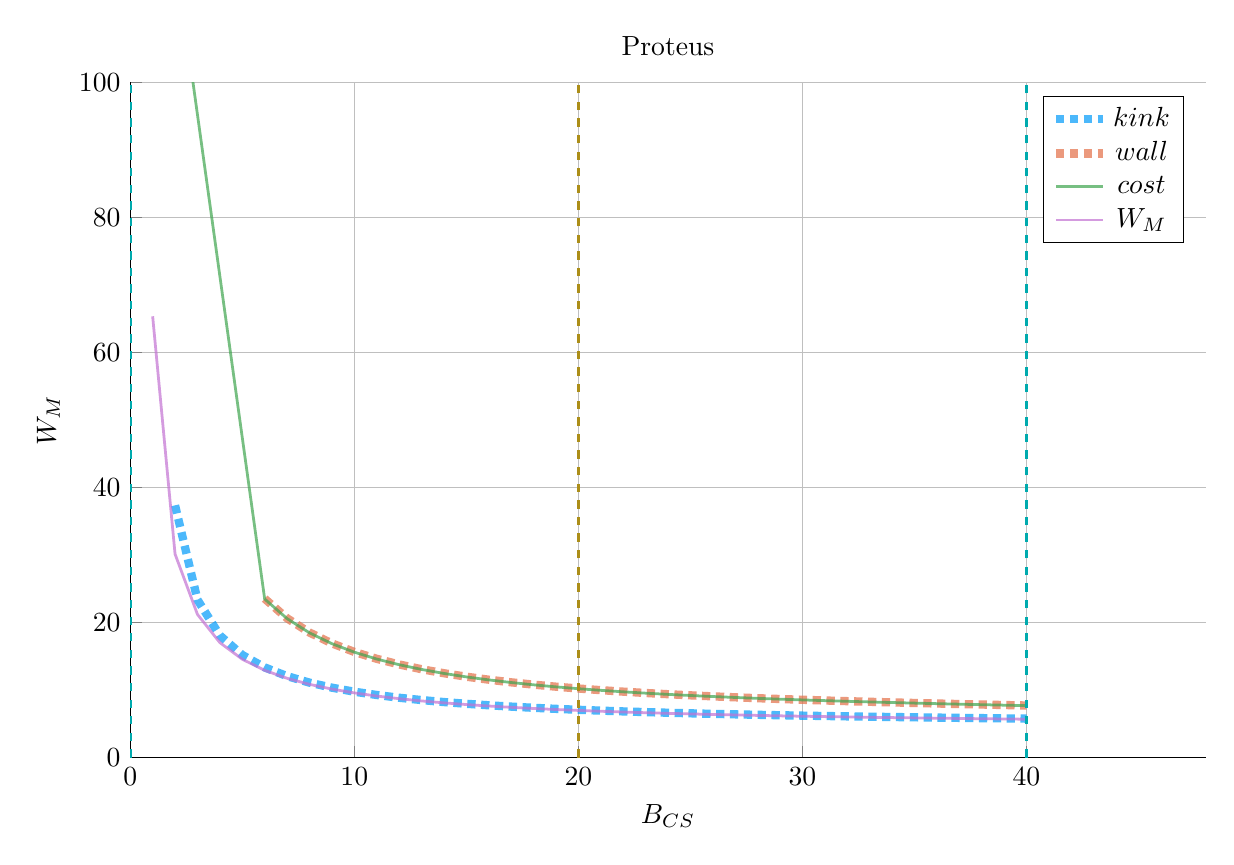
\begin{tikzpicture}[]
\begin{axis}[height = {101.6mm}, ylabel = {${W}_{M}$}, title = {Proteus}, xmin = {0.0}, xmax = {48.0}, ymax = {100.0}, xlabel = {${B}_{CS}$}, {unbounded coords=jump, scaled x ticks = false, xticklabel style={rotate = 0}, xmajorgrids = true, xtick = {0.0,10.0,20.0,30.0,40.0}, xticklabels = {0,10,20,30,40}, xtick align = inside, axis lines* = left, scaled y ticks = false, yticklabel style={rotate = 0}, ymajorgrids = true, ytick = {0.0,20.0,40.0,60.0,80.0,100.0}, yticklabels = {0,20,40,60,80,100}, ytick align = inside, axis lines* = left,     xshift = 0.0mm,
    yshift = 0.0mm,
    axis background/.style={fill={rgb,1:red,1.00000000;green,1.00000000;blue,1.00000000}}
, colorbar style={title=}}, ymin = {0.0}, width = {152.4mm}]\addplot+ [color = {rgb,1:red,0.00000000;green,0.60560316;blue,0.97868012},
draw opacity=0.7,
line width=3,
dotted,mark = none,
mark size = 2.0,
mark options = {
    color = {rgb,1:red,0.00000000;green,0.00000000;blue,0.00000000}, draw opacity = 0.7,
    fill = {rgb,1:red,0.00000000;green,0.60560316;blue,0.97868012}, fill opacity = 0.7,
    line width = 1,
    rotate = 0,
    solid
}]coordinates {
(2.0, 37.352716134550086)
(3.0, 23.372867608677893)
(4.0, 18.082969056077573)
(5.0, 15.20248682872566)
(6.0, 13.360048795601857)
(7.0, 12.068220612170562)
(8.0, 11.107021756467589)
(9.0, 10.361528417032178)
(10.0, 9.76538711385606)
(11.0, 9.277385884813329)
(12.0, 8.87045844192495)
(13.0, 8.526026311176693)
(14.0, 8.230871667306326)
(15.0, 7.975307275089902)
(16.0, 7.752051704511229)
(17.0, 7.55551626516457)
(18.0, 7.381329182247653)
(19.0, 7.226013408774766)
(20.0, 7.086768538488137)
(21.0, 6.961305946685665)
(22.0, 6.847736860963425)
(23.0, 6.744483725215405)
(24.0, 6.650222089868119)
(25.0, 6.563826322348436)
(26.0, 6.484335109054439)
(27.0, 6.4109217743956295)
(28.0, 6.34287136916924)
(29.0, 6.279562456405846)
(30.0, 6.220452497599473)
(31.0, 6.165066025474409)
(32.0, 6.11298521832458)
(33.0, 6.063841029942971)
(34.0, 6.017307885145791)
(35.0, 5.973097892102034)
(36.0, 5.930955507004097)
(37.0, 5.890653770007234)
(38.0, 5.85199197498705)
(39.0, 5.814791589808901)
(40.0, 5.778894374832782)
};
\addlegendentry{$kink$}
\addplot+ [color = {rgb,1:red,0.88887350;green,0.43564919;blue,0.27812294},
draw opacity=0.7,
line width=3,
dotted,mark = none,
mark size = 2.0,
mark options = {
    color = {rgb,1:red,0.00000000;green,0.00000000;blue,0.00000000}, draw opacity = 0.7,
    fill = {rgb,1:red,0.88887350;green,0.43564919;blue,0.27812294}, fill opacity = 0.7,
    line width = 1,
    rotate = 0,
    solid
}]coordinates {
(6.0, 23.539775020881077)
(7.0, 20.6320001321457)
(8.0, 18.521552626504068)
(9.0, 16.91717668670272)
(10.0, 15.655395334877854)
(11.0, 14.636976458282254)
(12.0, 13.798003046982357)
(13.0, 13.095339225722636)
(14.0, 12.498754821540345)
(15.0, 11.986393170450276)
(16.0, 11.542031521017869)
(17.0, 11.153355822447628)
(18.0, 10.810836000359506)
(19.0, 10.506970591915177)
(20.0, 10.235766195929521)
(21.0, 9.992370553981477)
(22.0, 9.772808716032094)
(23.0, 9.573789937689266)
(24.0, 9.392564086502505)
(25.0, 9.226813326462848)
(26.0, 9.074569347415679)
(27.0, 8.934149361981188)
(28.0, 8.804106072497458)
(29.0, 8.683188162252165)
(30.0, 8.570308800653658)
(31.0, 8.464520311489284)
(32.0, 8.364993623352605)
(33.0, 8.271001461166389)
(34.0, 8.181904486333885)
(35.0, 8.097139777010295)
(36.0, 8.016211177559283)
(37.0, 7.938681150182887)
(38.0, 7.86416384094757)
(39.0, 7.792319133366558)
(40.0, 7.722847509932094)
};
\addlegendentry{$wall$}
\addplot+ [color = {rgb,1:red,0.24222430;green,0.64327509;blue,0.30444865},
draw opacity=0.7,
line width=1,
solid,mark = none,
mark size = 2.0,
mark options = {
    color = {rgb,1:red,0.00000000;green,0.00000000;blue,0.00000000}, draw opacity = 0.7,
    fill = {rgb,1:red,0.24222430;green,0.64327509;blue,0.30444865}, fill opacity = 0.7,
    line width = 1,
    rotate = 0,
    solid
}]coordinates {
(1.0, 142.99282415442713)
(6.0, 23.485589275905202)
(7.0, 20.583617680434923)
(8.0, 18.477480950488083)
(9.0, 16.876434508028233)
(10.0, 15.61730160769167)
(11.0, 14.6010383114463)
(12.0, 13.763851803793637)
(13.0, 13.062691421921969)
(14.0, 12.467387968434226)
(15.0, 11.956129155164682)
(16.0, 11.512725769754612)
(17.0, 11.124889356884182)
(18.0, 10.78310976790515)
(19.0, 10.479901535174305)
(20.0, 10.209283873179716)
(21.0, 9.966414997938033)
(22.0, 9.747328453115049)
(23.0, 9.548740761808915)
(24.0, 9.3679076006721)
(25.0, 9.20251640114714)
(26.0, 9.05060297162576)
(27.0, 8.910488348162888)
(28.0, 8.780728417974629)
(29.0, 8.660074609796615)
(30.0, 8.547442559708593)
(31.0, 8.441886634212462)
(32.0, 8.342579576538721)
(33.0, 8.248795785080748)
(34.0, 8.159897358494677)
(35.0, 8.07532253868397)
(36.0, 7.9945762899445185)
(37.0, 7.917222117737104)
(38.0, 7.84287488878461)
(39.0, 7.771195220941283)
(40.0, 7.70188433978773)
};
\addlegendentry{$cost$}
\addplot+ [color = {rgb,1:red,0.76444018;green,0.44411178;blue,0.82429754},
draw opacity=0.7,
line width=1,
solid,mark = none,
mark size = 2.0,
mark options = {
    color = {rgb,1:red,0.00000000;green,0.00000000;blue,0.00000000}, draw opacity = 0.7,
    fill = {rgb,1:red,0.76444018;green,0.44411178;blue,0.82429754}, fill opacity = 0.7,
    line width = 1,
    rotate = 0,
    solid
}]coordinates {
(1.0, 65.34155060768514)
(2.0, 30.1396998290261)
(3.0, 21.20631400241935)
(4.0, 17.031733361268905)
(5.0, 14.569846532592615)
(6.0, 12.92838858361226)
(7.0, 11.747935636375395)
(8.0, 10.854761799937048)
(9.0, 10.153457025039408)
(10.0, 9.587712682509892)
(11.0, 9.121118498094127)
(12.0, 8.729954207268294)
(13.0, 8.397249636791653)
(14.0, 8.111029493345612)
(15.0, 7.862296804332222)
(16.0, 7.644402111831462)
(17.0, 7.452065437086496)
(18.0, 7.281174212102364)
(19.0, 7.128455611694994)
(20.0, 6.991275094865535)
(21.0, 6.867485398134194)
(22.0, 6.755230934308156)
(23.0, 6.6529345555822195)
(24.0, 6.559553129935918)
(25.0, 6.473692619754001)
(26.0, 6.394660734853869)
(27.0, 6.321656158752529)
(28.0, 6.253886397075824)
(29.0, 6.19081500501821)
(30.0, 6.131814020485674)
(31.0, 6.076616951082212)
(32.0, 6.024623729762463)
(33.0, 5.9755547119435315)
(34.0, 5.9291530074992895)
(35.0, 5.885014491486683)
(36.0, 5.842965715961846)
(37.0, 5.8027768609843235)
(38.0, 5.764251375308554)
(39.0, 5.7272021864970775)
(40.0, 5.691504716134858)
};
\addlegendentry{$W_M$}
\addplot+ [color = {rgb,1:red,0.67554396;green,0.55566233;blue,0.09423434},
draw opacity=1.0,
line width=1,
dashed,mark = none,
mark size = 2.0,
mark options = {
    color = {rgb,1:red,0.00000000;green,0.00000000;blue,0.00000000}, draw opacity = 1.0,
    fill = {rgb,1:red,0.67554396;green,0.55566233;blue,0.09423434}, fill opacity = 1.0,
    line width = 1,
    rotate = 0,
    solid
},forget plot]coordinates {
(20.0, 0.0)
(20.0, 100.0)
};
\addplot+ [color = {rgb,1:red,0.00000048;green,0.66575898;blue,0.68099695},
draw opacity=1.0,
line width=1,
dashed,mark = none,
mark size = 2.0,
mark options = {
    color = {rgb,1:red,0.00000000;green,0.00000000;blue,0.00000000}, draw opacity = 1.0,
    fill = {rgb,1:red,0.00000048;green,0.66575898;blue,0.68099695}, fill opacity = 1.0,
    line width = 1,
    rotate = 0,
    solid
},forget plot]coordinates {
(0.0, 0.0)
(0.0, 100.0)
};
\addplot+ [color = {rgb,1:red,0.00000048;green,0.66575898;blue,0.68099695},
draw opacity=1.0,
line width=1,
dashed,mark = none,
mark size = 2.0,
mark options = {
    color = {rgb,1:red,0.00000000;green,0.00000000;blue,0.00000000}, draw opacity = 1.0,
    fill = {rgb,1:red,0.00000048;green,0.66575898;blue,0.68099695}, fill opacity = 1.0,
    line width = 1,
    rotate = 0,
    solid
},forget plot]coordinates {
(40.0, 0.0)
(40.0, 100.0)
};
\end{axis}

\end{tikzpicture}

    \end{adjustbox}
        \caption{Proteus Capital Cost}
    \end{subfigure}
    \hfill
    \begin{subfigure}[t]{0.45\textwidth}
        \centering
    \begin{adjustbox}{width=\textwidth}
      \Large
      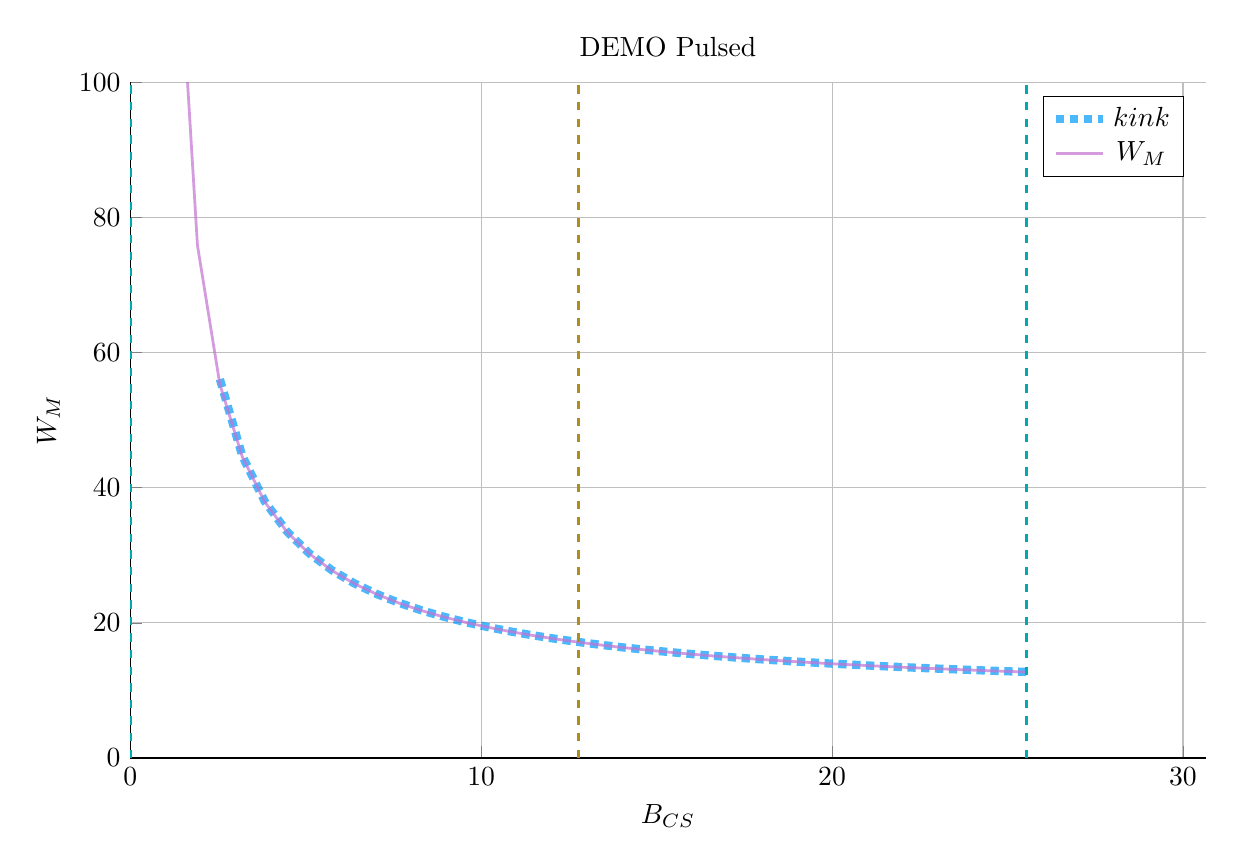
\begin{tikzpicture}[]
\begin{axis}[height = {101.6mm}, ylabel = {${W}_{M}$}, title = {DEMO Pulsed}, xmin = {0.0}, xmax = {30.647999999999996}, ymax = {100.0}, xlabel = {${B}_{CS}$}, {unbounded coords=jump, scaled x ticks = false, xticklabel style={rotate = 0}, xmajorgrids = true, xtick = {0.0,10.0,20.0,30.0}, xticklabels = {0,10,20,30}, xtick align = inside, axis lines* = left, scaled y ticks = false, yticklabel style={rotate = 0}, ymajorgrids = true, ytick = {0.0,20.0,40.0,60.0,80.0,100.0}, yticklabels = {0,20,40,60,80,100}, ytick align = inside, axis lines* = left,     xshift = 0.0mm,
    yshift = 0.0mm,
    axis background/.style={fill={rgb,1:red,1.00000000;green,1.00000000;blue,1.00000000}}
, colorbar style={title=}}, ymin = {0.0}, width = {152.4mm}]\addplot+ [color = {rgb,1:red,0.00000000;green,0.60560316;blue,0.97868012},
draw opacity=0.7,
line width=3,
dotted,mark = none,
mark size = 2.0,
mark options = {
    color = {rgb,1:red,0.00000000;green,0.00000000;blue,0.00000000}, draw opacity = 0.7,
    fill = {rgb,1:red,0.00000000;green,0.60560316;blue,0.97868012}, fill opacity = 0.7,
    line width = 1,
    rotate = 0,
    solid
}]coordinates {
(2.554, 56.07719132875428)
(3.1925, 44.70978735818654)
(3.831, 37.988804737609954)
(4.4695, 33.496637725626464)
(5.108, 30.25557091641782)
(5.7465, 27.792084909829864)
(6.385, 25.847698616953984)
(7.0235, 24.26870740237538)
(7.662, 22.957634145310223)
(8.3005, 21.849475745180996)
(8.939, 20.8991014117893)
(9.5775, 20.074123603397076)
(10.216, 19.350648410482226)
(10.8545, 18.71062990061846)
(11.493, 18.14016149214523)
(12.1315, 17.628337293215974)
(12.77, 17.166473566094577)
(13.4085, 16.747555956157687)
(14.047, 16.365859907242562)
(14.6855, 16.01665516516569)
(15.324, 15.69599151025235)
(15.9625, 15.400550163564295)
(16.601, 15.127514152010027)
(17.2395, 14.874476070125503)
(17.878, 14.639361958039018)
(18.5165, 14.420383545361142)
(19.155, 14.215976454606855)
(19.7935, 14.024773313662244)
(20.432, 13.84557329418479)
(21.0705, 13.677306042635895)
(21.709, 13.519034266108502)
(22.3475, 13.369916027516416)
(22.986, 13.229192567054229)
(23.6245, 13.096195240500935)
(24.263, 12.970308060981914)
(24.9015, 12.850987074408986)
(25.54, 12.737727596814343)
};
\addlegendentry{$kink$}
\addplot+ [color = {rgb,1:red,0.76444018;green,0.44411178;blue,0.82429754},
draw opacity=0.7,
line width=1,
solid,mark = none,
mark size = 2.0,
mark options = {
    color = {rgb,1:red,0.00000000;green,0.00000000;blue,0.00000000}, draw opacity = 0.7,
    fill = {rgb,1:red,0.76444018;green,0.44411178;blue,0.82429754}, fill opacity = 0.7,
    line width = 1,
    rotate = 0,
    solid
}]coordinates {
(1.277, 130.40706024791734)
(1.9155, 75.88512258940752)
(2.554, 55.316757608952784)
(3.1925, 44.59467119661246)
(3.831, 37.928300802944165)
(4.4695, 33.44504682714259)
(5.108, 30.2101384502726)
(5.7465, 27.751178232691146)
(6.385, 25.81026716048573)
(7.0235, 24.234033460451204)
(7.662, 22.925204299162786)
(8.3005, 21.81890952309676)
(8.939, 20.870108279005954)
(9.5775, 20.046476622347228)
(10.216, 19.324166359349746)
(10.8545, 18.685166010834994)
(11.493, 18.115594934733192)
(12.1315, 17.60456729376528)
(12.77, 17.14341399674411)
(13.4085, 16.725136862339944)
(14.047, 16.34401819290831)
(14.6855, 15.995334981567458)
(15.324, 15.675148109309111)
(15.9625, 15.38014257310665)
(16.601, 15.107506335019977)
(17.2395, 14.854836171949092)
(17.878, 14.620064127853686)
(18.5165, 14.401399811466803)
(19.155, 14.197284002303897)
(19.7935, 14.006351608513064)
(20.432, 13.827401551536152)
(21.0705, 13.659372012090312)
(21.709, 13.501320519301304)
(22.3475, 13.3524067154305)
(22.986, 13.211878951832537)
(23.6245, 13.079062267577786)
(24.263, 12.953348383803398)
(24.9015, 12.834187990844306)
(25.54, 12.721083008291227)
};
\addlegendentry{$W_M$}
\addplot+ [color = {rgb,1:red,0.67554396;green,0.55566233;blue,0.09423434},
draw opacity=1.0,
line width=1,
dashed,mark = none,
mark size = 2.0,
mark options = {
    color = {rgb,1:red,0.00000000;green,0.00000000;blue,0.00000000}, draw opacity = 1.0,
    fill = {rgb,1:red,0.67554396;green,0.55566233;blue,0.09423434}, fill opacity = 1.0,
    line width = 1,
    rotate = 0,
    solid
},forget plot]coordinates {
(12.77, 0.0)
(12.77, 100.0)
};
\addplot+ [color = {rgb,1:red,0.00000048;green,0.66575898;blue,0.68099695},
draw opacity=1.0,
line width=1,
dashed,mark = none,
mark size = 2.0,
mark options = {
    color = {rgb,1:red,0.00000000;green,0.00000000;blue,0.00000000}, draw opacity = 1.0,
    fill = {rgb,1:red,0.00000048;green,0.66575898;blue,0.68099695}, fill opacity = 1.0,
    line width = 1,
    rotate = 0,
    solid
},forget plot]coordinates {
(0.0, 0.0)
(0.0, 100.0)
};
\addplot+ [color = {rgb,1:red,0.00000048;green,0.66575898;blue,0.68099695},
draw opacity=1.0,
line width=1,
dashed,mark = none,
mark size = 2.0,
mark options = {
    color = {rgb,1:red,0.00000000;green,0.00000000;blue,0.00000000}, draw opacity = 1.0,
    fill = {rgb,1:red,0.00000048;green,0.66575898;blue,0.68099695}, fill opacity = 1.0,
    line width = 1,
    rotate = 0,
    solid
},forget plot]coordinates {
(25.54, 0.0)
(25.54, 100.0)
};
\end{axis}

\end{tikzpicture}

    \end{adjustbox}
        \caption{DEMO Pulsed Capital Cost}
    \end{subfigure}
    \hfill \hfill ~\\ ~\\ ~\\
    \hfill
    \begin{subfigure}[t]{0.45\textwidth}
        \centering
    \begin{adjustbox}{width=\textwidth}
      \Large
      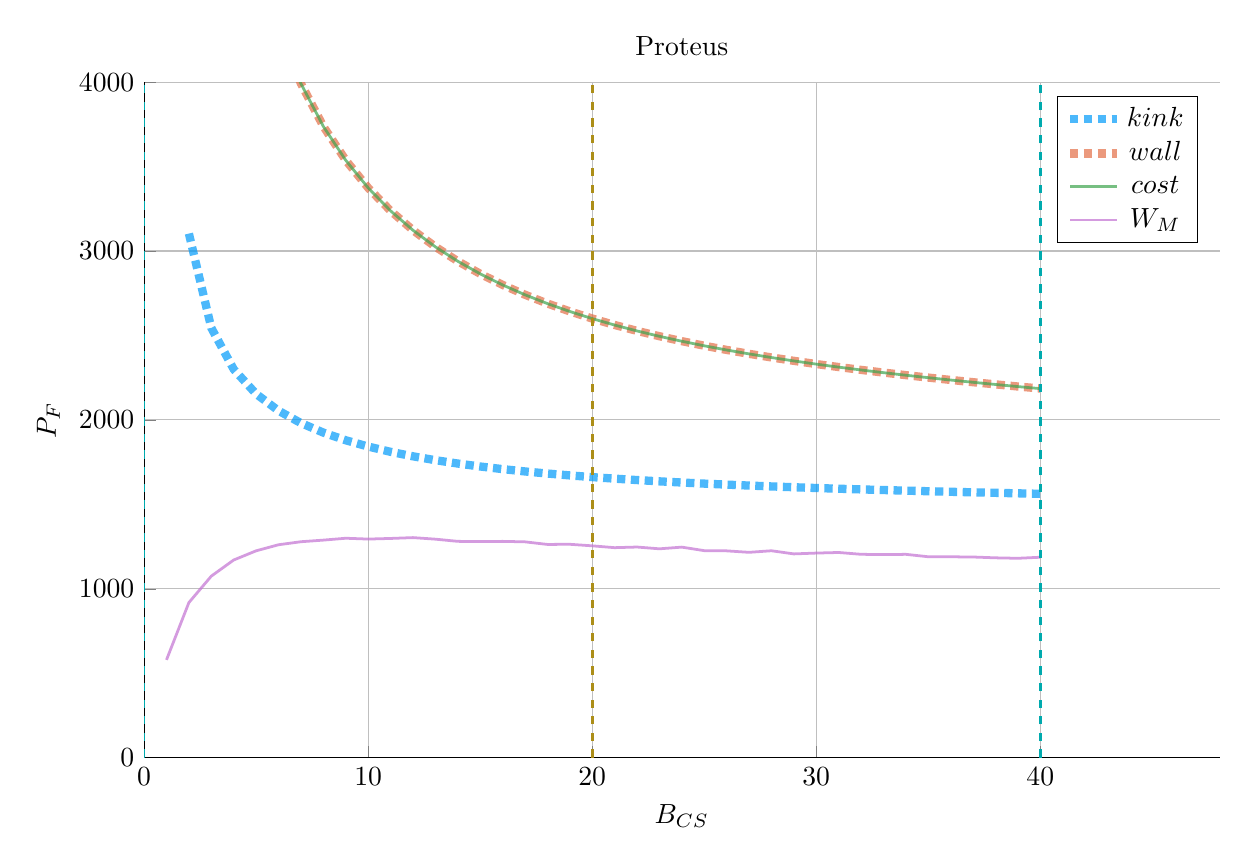
\begin{tikzpicture}[]
\begin{axis}[height = {101.6mm}, ylabel = {${P}_{F}$}, title = {Proteus}, xmin = {0.0}, xmax = {48.0}, ymax = {4000.0}, xlabel = {${B}_{CS}$}, {unbounded coords=jump, scaled x ticks = false, xticklabel style={rotate = 0}, xmajorgrids = true, xtick = {0.0,10.0,20.0,30.0,40.0}, xticklabels = {0,10,20,30,40}, xtick align = inside, axis lines* = left, scaled y ticks = false, yticklabel style={rotate = 0}, ymajorgrids = true, ytick = {0.0,1000.0,2000.0,3000.0,4000.0}, yticklabels = {0,1000,2000,3000,4000}, ytick align = inside, axis lines* = left,     xshift = 0.0mm,
    yshift = 0.0mm,
    axis background/.style={fill={rgb,1:red,1.00000000;green,1.00000000;blue,1.00000000}}
, colorbar style={title=}}, ymin = {0.0}, width = {152.4mm}]\addplot+ [color = {rgb,1:red,0.00000000;green,0.60560316;blue,0.97868012},
draw opacity=0.7,
line width=3,
dotted,mark = none,
mark size = 2.0,
mark options = {
    color = {rgb,1:red,0.00000000;green,0.00000000;blue,0.00000000}, draw opacity = 0.7,
    fill = {rgb,1:red,0.00000000;green,0.60560316;blue,0.97868012}, fill opacity = 0.7,
    line width = 1,
    rotate = 0,
    solid
}]coordinates {
(2.0, 3103.446964483028)
(3.0, 2544.8446560898697)
(4.0, 2299.7883505862683)
(5.0, 2153.9401008014215)
(6.0, 2054.566085735622)
(7.0, 1981.4265807089412)
(8.0, 1924.8436783738584)
(9.0, 1879.5196356674505)
(10.0, 1842.2729246450338)
(11.0, 1811.058926720514)
(12.0, 1784.4936387453804)
(13.0, 1761.6008925896194)
(14.0, 1741.6687589347825)
(15.0, 1724.1634290251588)
(16.0, 1708.675049552884)
(17.0, 1694.8827715321645)
(18.0, 1682.530881991843)
(19.0, 1671.41236950268)
(20.0, 1661.3577430103219)
(21.0, 1652.2262595201232)
(22.0, 1643.9000207526378)
(23.0, 1636.2791174294293)
(24.0, 1629.2785569006053)
(25.0, 1622.8251506662725)
(26.0, 1616.8556306952612)
(27.0, 1611.314956936522)
(28.0, 1606.1550041060862)
(29.0, 1601.3335066156708)
(30.0, 1596.813203261599)
(31.0, 1592.5611379345382)
(32.0, 1588.5481006380803)
(33.0, 1584.7480767592144)
(34.0, 1581.137944358817)
(35.0, 1577.697113913979)
(36.0, 1574.4071855210084)
(37.0, 1571.2517143488374)
(38.0, 1568.2160778261118)
(39.0, 1565.2871970827582)
(40.0, 1562.4534231467098)
};
\addlegendentry{$kink$}
\addplot+ [color = {rgb,1:red,0.88887350;green,0.43564919;blue,0.27812294},
draw opacity=0.7,
line width=3,
dotted,mark = none,
mark size = 2.0,
mark options = {
    color = {rgb,1:red,0.00000000;green,0.00000000;blue,0.00000000}, draw opacity = 0.7,
    fill = {rgb,1:red,0.88887350;green,0.43564919;blue,0.27812294}, fill opacity = 0.7,
    line width = 1,
    rotate = 0,
    solid
}]coordinates {
(6.0, 4323.6250098364)
(7.0, 3991.769889747364)
(8.0, 3738.5019719471065)
(9.0, 3537.844669896544)
(10.0, 3374.4482917260734)
(11.0, 3238.5755547510726)
(12.0, 3123.707522754923)
(13.0, 3025.2906069442192)
(14.0, 2940.0327020869304)
(15.0, 2865.4848852505193)
(16.0, 2799.781119223045)
(17.0, 2741.4699493813873)
(18.0, 2689.4020933235506)
(19.0, 2642.653242662454)
(20.0, 2600.4697515783287)
(21.0, 2562.2296107375905)
(22.0, 2527.4138764273603)
(23.0, 2495.5854037525905)
(24.0, 2466.372779394115)
(25.0, 2439.458018649117)
(26.0, 2414.5670292139203)
(27.0, 2391.4621364565396)
(28.0, 2369.9361636649223)
(29.0, 2349.807698422879)
(30.0, 2330.917272823136)
(31.0, 2313.1242542242217)
(32.0, 2296.3042930448983)
(33.0, 2280.3472105413966)
(34.0, 2265.1552364984454)
(35.0, 2250.64152696625)
(36.0, 2236.728907456072)
(37.0, 2223.34879867789)
(38.0, 2210.440290899089)
(39.0, 2197.9493399942594)
(40.0, 2185.8280637304556)
};
\addlegendentry{$wall$}
\addplot+ [color = {rgb,1:red,0.24222430;green,0.64327509;blue,0.30444865},
draw opacity=0.7,
line width=1,
solid,mark = none,
mark size = 2.0,
mark options = {
    color = {rgb,1:red,0.00000000;green,0.00000000;blue,0.00000000}, draw opacity = 0.7,
    fill = {rgb,1:red,0.24222430;green,0.64327509;blue,0.30444865}, fill opacity = 0.7,
    line width = 1,
    rotate = 0,
    solid
}]coordinates {
(6.0, 4323.626574700694)
(7.0, 3991.6631892643886)
(8.0, 3738.320677711505)
(9.0, 3537.608432111376)
(10.0, 3374.169551170435)
(11.0, 3238.26268518392)
(12.0, 3123.3664382128786)
(13.0, 3024.925648281227)
(14.0, 2939.6471637487452)
(15.0, 2865.0813351410798)
(16.0, 2799.36161050096)
(17.0, 2741.036157991272)
(18.0, 2688.955412764389)
(19.0, 2642.1948546153712)
(20.0, 2600.0006699519377)
(21.0, 2561.750720954071)
(22.0, 2526.9259593565384)
(23.0, 2495.0891597848504)
(24.0, 2465.868837737165)
(25.0, 2438.946956709572)
(26.0, 2414.0493736799453)
(27.0, 2390.9383771738217)
(28.0, 2369.4067567095603)
(29.0, 2349.2730703154293)
(30.0, 2330.3778259957894)
(31.0, 2312.580367156535)
(32.0, 2295.756323266687)
(33.0, 2279.7954985113834)
(34.0, 2264.600106129103)
(35.0, 2250.0832841784704)
(36.0, 2236.1678437242876)
(37.0, 2222.7851932488634)
(38.0, 2209.8744060154622)
(39.0, 2197.3814243621327)
(40.0, 2185.25835564655)
};
\addlegendentry{$cost$}
\addplot+ [color = {rgb,1:red,0.76444018;green,0.44411178;blue,0.82429754},
draw opacity=0.7,
line width=1,
solid,mark = none,
mark size = 2.0,
mark options = {
    color = {rgb,1:red,0.00000000;green,0.00000000;blue,0.00000000}, draw opacity = 0.7,
    fill = {rgb,1:red,0.76444018;green,0.44411178;blue,0.82429754}, fill opacity = 0.7,
    line width = 1,
    rotate = 0,
    solid
}]coordinates {
(1.0, 579.1770635549526)
(2.0, 918.4032254393342)
(3.0, 1074.9224453723655)
(4.0, 1170.511694377957)
(5.0, 1224.8328861528692)
(6.0, 1260.7420812438745)
(7.0, 1278.6558574628261)
(8.0, 1288.1834994000776)
(9.0, 1299.316367656194)
(10.0, 1294.3919774035123)
(11.0, 1298.0825023461)
(12.0, 1303.0515424091216)
(13.0, 1293.865250965231)
(14.0, 1280.9007331366447)
(15.0, 1279.4372391236866)
(16.0, 1280.7616167001067)
(17.0, 1277.9826713878344)
(18.0, 1262.6816701784642)
(19.0, 1263.51658245539)
(20.0, 1254.3696077727395)
(21.0, 1243.4883851017005)
(22.0, 1247.271738332874)
(23.0, 1236.6841019289109)
(24.0, 1246.6992139316376)
(25.0, 1225.840796579752)
(26.0, 1224.5924675745566)
(27.0, 1215.860267902309)
(28.0, 1225.2315346432224)
(29.0, 1206.5608956425033)
(30.0, 1211.487449032281)
(31.0, 1214.9842647989544)
(32.0, 1204.193043008769)
(33.0, 1202.3951421040542)
(34.0, 1204.0095118625998)
(35.0, 1189.6936123071723)
(36.0, 1189.4184409015577)
(37.0, 1188.1807853881828)
(38.0, 1183.3067663347506)
(39.0, 1180.5861451931135)
(40.0, 1186.8241154535017)
};
\addlegendentry{$W_M$}
\addplot+ [color = {rgb,1:red,0.67554396;green,0.55566233;blue,0.09423434},
draw opacity=1.0,
line width=1,
dashed,mark = none,
mark size = 2.0,
mark options = {
    color = {rgb,1:red,0.00000000;green,0.00000000;blue,0.00000000}, draw opacity = 1.0,
    fill = {rgb,1:red,0.67554396;green,0.55566233;blue,0.09423434}, fill opacity = 1.0,
    line width = 1,
    rotate = 0,
    solid
},forget plot]coordinates {
(20.0, 0.0)
(20.0, 4000.0)
};
\addplot+ [color = {rgb,1:red,0.00000048;green,0.66575898;blue,0.68099695},
draw opacity=1.0,
line width=1,
dashed,mark = none,
mark size = 2.0,
mark options = {
    color = {rgb,1:red,0.00000000;green,0.00000000;blue,0.00000000}, draw opacity = 1.0,
    fill = {rgb,1:red,0.00000048;green,0.66575898;blue,0.68099695}, fill opacity = 1.0,
    line width = 1,
    rotate = 0,
    solid
},forget plot]coordinates {
(0.0, 0.0)
(0.0, 4000.0)
};
\addplot+ [color = {rgb,1:red,0.00000048;green,0.66575898;blue,0.68099695},
draw opacity=1.0,
line width=1,
dashed,mark = none,
mark size = 2.0,
mark options = {
    color = {rgb,1:red,0.00000000;green,0.00000000;blue,0.00000000}, draw opacity = 1.0,
    fill = {rgb,1:red,0.00000048;green,0.66575898;blue,0.68099695}, fill opacity = 1.0,
    line width = 1,
    rotate = 0,
    solid
},forget plot]coordinates {
(40.0, 0.0)
(40.0, 4000.0)
};
\end{axis}

\end{tikzpicture}

    \end{adjustbox}
        \caption{Proteus Fusion Power}
    \end{subfigure}
    \hfill
    \begin{subfigure}[t]{0.45\textwidth}
        \centering
    \begin{adjustbox}{width=\textwidth}
      \Large
      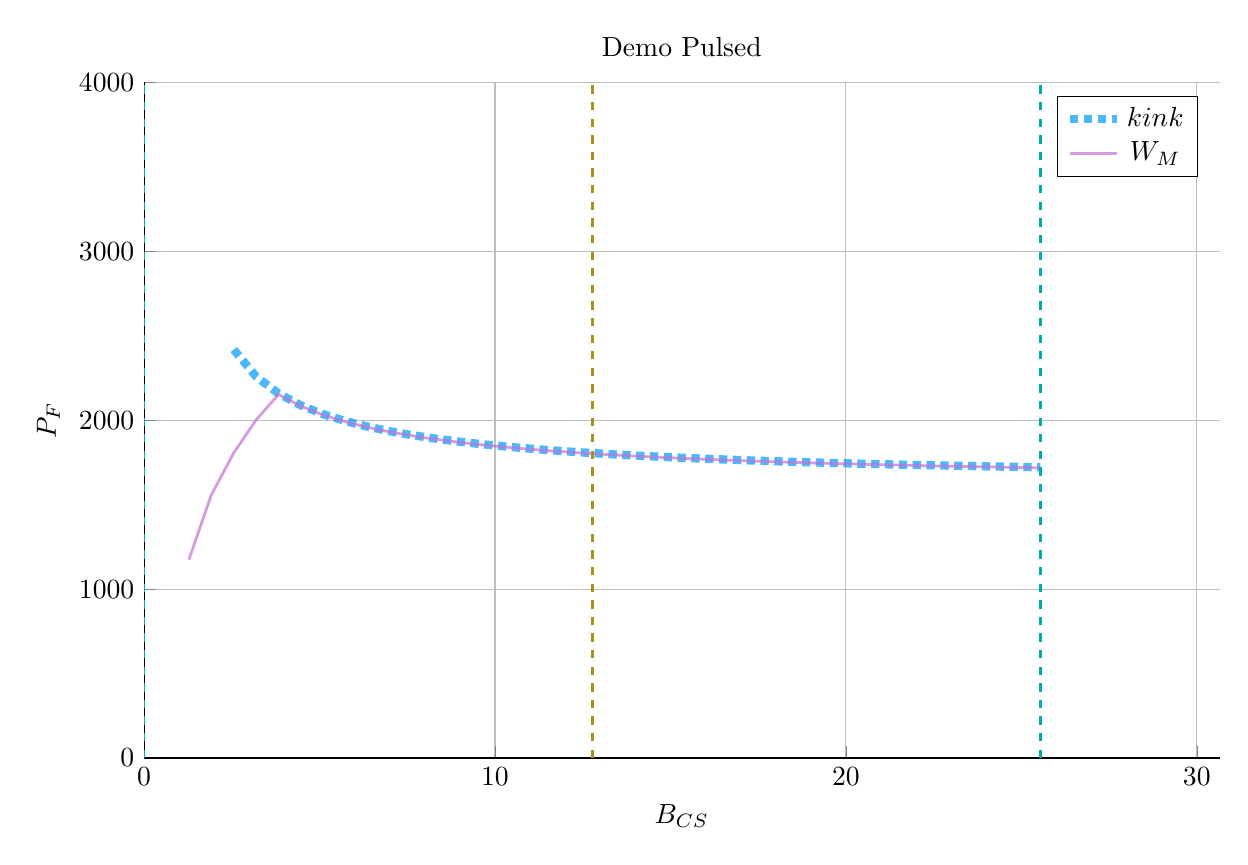
\begin{tikzpicture}[]
\begin{axis}[height = {101.6mm}, ylabel = {${P}_{F}$}, title = {Demo Pulsed}, xmin = {0.0}, xmax = {30.647999999999996}, ymax = {4000.0}, xlabel = {${B}_{CS}$}, {unbounded coords=jump, scaled x ticks = false, xticklabel style={rotate = 0}, xmajorgrids = true, xtick = {0.0,10.0,20.0,30.0}, xticklabels = {0,10,20,30}, xtick align = inside, axis lines* = left, scaled y ticks = false, yticklabel style={rotate = 0}, ymajorgrids = true, ytick = {0.0,1000.0,2000.0,3000.0,4000.0}, yticklabels = {0,1000,2000,3000,4000}, ytick align = inside, axis lines* = left,     xshift = 0.0mm,
    yshift = 0.0mm,
    axis background/.style={fill={rgb,1:red,1.00000000;green,1.00000000;blue,1.00000000}}
, colorbar style={title=}}, ymin = {0.0}, width = {152.4mm}]\addplot+ [color = {rgb,1:red,0.00000000;green,0.60560316;blue,0.97868012},
draw opacity=0.7,
line width=3,
dotted,mark = none,
mark size = 2.0,
mark options = {
    color = {rgb,1:red,0.00000000;green,0.00000000;blue,0.00000000}, draw opacity = 0.7,
    fill = {rgb,1:red,0.00000000;green,0.60560316;blue,0.97868012}, fill opacity = 0.7,
    line width = 1,
    rotate = 0,
    solid
}]coordinates {
(2.554, 2418.439490660037)
(3.1925, 2258.667693929749)
(3.831, 2158.0434330029475)
(4.4695, 2087.6944206835706)
(5.108, 2035.1850409704718)
(5.7465, 1994.1965229213151)
(6.385, 1961.1441091669103)
(7.0235, 1933.826748790783)
(7.662, 1910.809955252131)
(8.3005, 1891.1142191277927)
(8.939, 1874.045166007475)
(9.5775, 1859.0951637532023)
(10.216, 1845.8834195623997)
(10.8545, 1834.1179730892675)
(11.493, 1823.5707253838252)
(12.1315, 1814.0605347693095)
(12.77, 1805.4414957120475)
(13.4085, 1797.5944815414484)
(14.047, 1790.4213179193448)
(14.6855, 1783.840134166425)
(15.324, 1777.781969664348)
(15.9625, 1772.1884340879249)
(16.601, 1767.0095972933589)
(17.2395, 1762.2024944996933)
(17.878, 1757.7298713228834)
(18.5165, 1753.5594201574)
(19.155, 1749.6627140975622)
(19.7935, 1746.0147788945287)
(20.432, 1742.5935778099401)
(21.0705, 1739.3793742056532)
(21.709, 1736.35482098222)
(22.3475, 1733.5042719541648)
(22.986, 1730.8135737806701)
(23.6245, 1728.2702184672714)
(24.263, 1725.8626428941761)
(24.9015, 1723.5806118852602)
(25.54, 1721.4146017114554)
};
\addlegendentry{$kink$}
\addplot+ [color = {rgb,1:red,0.76444018;green,0.44411178;blue,0.82429754},
draw opacity=0.7,
line width=1,
solid,mark = none,
mark size = 2.0,
mark options = {
    color = {rgb,1:red,0.00000000;green,0.00000000;blue,0.00000000}, draw opacity = 0.7,
    fill = {rgb,1:red,0.76444018;green,0.44411178;blue,0.82429754}, fill opacity = 0.7,
    line width = 1,
    rotate = 0,
    solid
}]coordinates {
(1.277, 1174.4191595640114)
(1.9155, 1557.5099838793772)
(2.554, 1806.3330313588413)
(3.1925, 2002.266281526456)
(3.831, 2152.948912848028)
(4.4695, 2082.9342814002794)
(5.108, 2030.6738841896818)
(5.7465, 1989.8799521445594)
(6.385, 1956.9849582412296)
(7.0235, 1929.7982968068923)
(7.662, 1906.8921995146331)
(8.3005, 1887.2917453417733)
(8.939, 1870.3057585821527)
(9.5775, 1855.4289762406506)
(10.216, 1842.2823256076385)
(10.8545, 1830.575224059819)
(11.493, 1820.0806153930123)
(12.1315, 1810.6181808889562)
(12.77, 1802.0426638004947)
(13.4085, 1794.2355420887463)
(14.047, 1787.0990590472247)
(14.6855, 1780.5516755814833)
(15.324, 1774.524841644359)
(15.9625, 1768.9603836664687)
(16.601, 1763.8086152609226)
(17.2395, 1759.0267819242679)
(17.878, 1754.5778384698829)
(18.5165, 1750.4295358069392)
(19.155, 1746.5536228804472)
(19.7935, 1742.9252430663948)
(20.432, 1739.5224273045656)
(21.0705, 1736.3256505161612)
(21.709, 1733.3175403646217)
(22.3475, 1730.482506673844)
(22.986, 1727.8065934950305)
(23.6245, 1725.2772187330588)
(24.263, 1722.8829728498188)
(24.9015, 1720.6135803737259)
(25.54, 1718.4596602703402)
};
\addlegendentry{$W_M$}
\addplot+ [color = {rgb,1:red,0.67554396;green,0.55566233;blue,0.09423434},
draw opacity=1.0,
line width=1,
dashed,mark = none,
mark size = 2.0,
mark options = {
    color = {rgb,1:red,0.00000000;green,0.00000000;blue,0.00000000}, draw opacity = 1.0,
    fill = {rgb,1:red,0.67554396;green,0.55566233;blue,0.09423434}, fill opacity = 1.0,
    line width = 1,
    rotate = 0,
    solid
},forget plot]coordinates {
(12.77, 0.0)
(12.77, 4000.0)
};
\addplot+ [color = {rgb,1:red,0.00000048;green,0.66575898;blue,0.68099695},
draw opacity=1.0,
line width=1,
dashed,mark = none,
mark size = 2.0,
mark options = {
    color = {rgb,1:red,0.00000000;green,0.00000000;blue,0.00000000}, draw opacity = 1.0,
    fill = {rgb,1:red,0.00000048;green,0.66575898;blue,0.68099695}, fill opacity = 1.0,
    line width = 1,
    rotate = 0,
    solid
},forget plot]coordinates {
(0.0, 0.0)
(0.0, 4000.0)
};
\addplot+ [color = {rgb,1:red,0.00000048;green,0.66575898;blue,0.68099695},
draw opacity=1.0,
line width=1,
dashed,mark = none,
mark size = 2.0,
mark options = {
    color = {rgb,1:red,0.00000000;green,0.00000000;blue,0.00000000}, draw opacity = 1.0,
    fill = {rgb,1:red,0.00000048;green,0.66575898;blue,0.68099695}, fill opacity = 1.0,
    line width = 1,
    rotate = 0,
    solid
},forget plot]coordinates {
(25.54, 0.0)
(25.54, 4000.0)
};
\end{axis}

\end{tikzpicture}

    \end{adjustbox}
        \caption{DEMO Pulsed Fusion Power}
    \end{subfigure}
    \hfill \hfill ~\\ ~\\ ~\\
    \caption{Pulsed $B_{CS}$ Sensitivities}
    \label{fig:pulsed_sensitivities} ~ \\
    \small{ Pulsed machines become more economically attractive as their central solenoid is strengthened. However as these plots show, the positive benefits of this have rapidly diminishing returns. HTS tape's magnet range happens to be inside regime. }
\end{figure*}

\begin{figure*}
    \centering
    \hfill
    \begin{subfigure}[t]{0.45\textwidth}
        \centering
		\begin{adjustbox}{width=\textwidth}
			\Large
			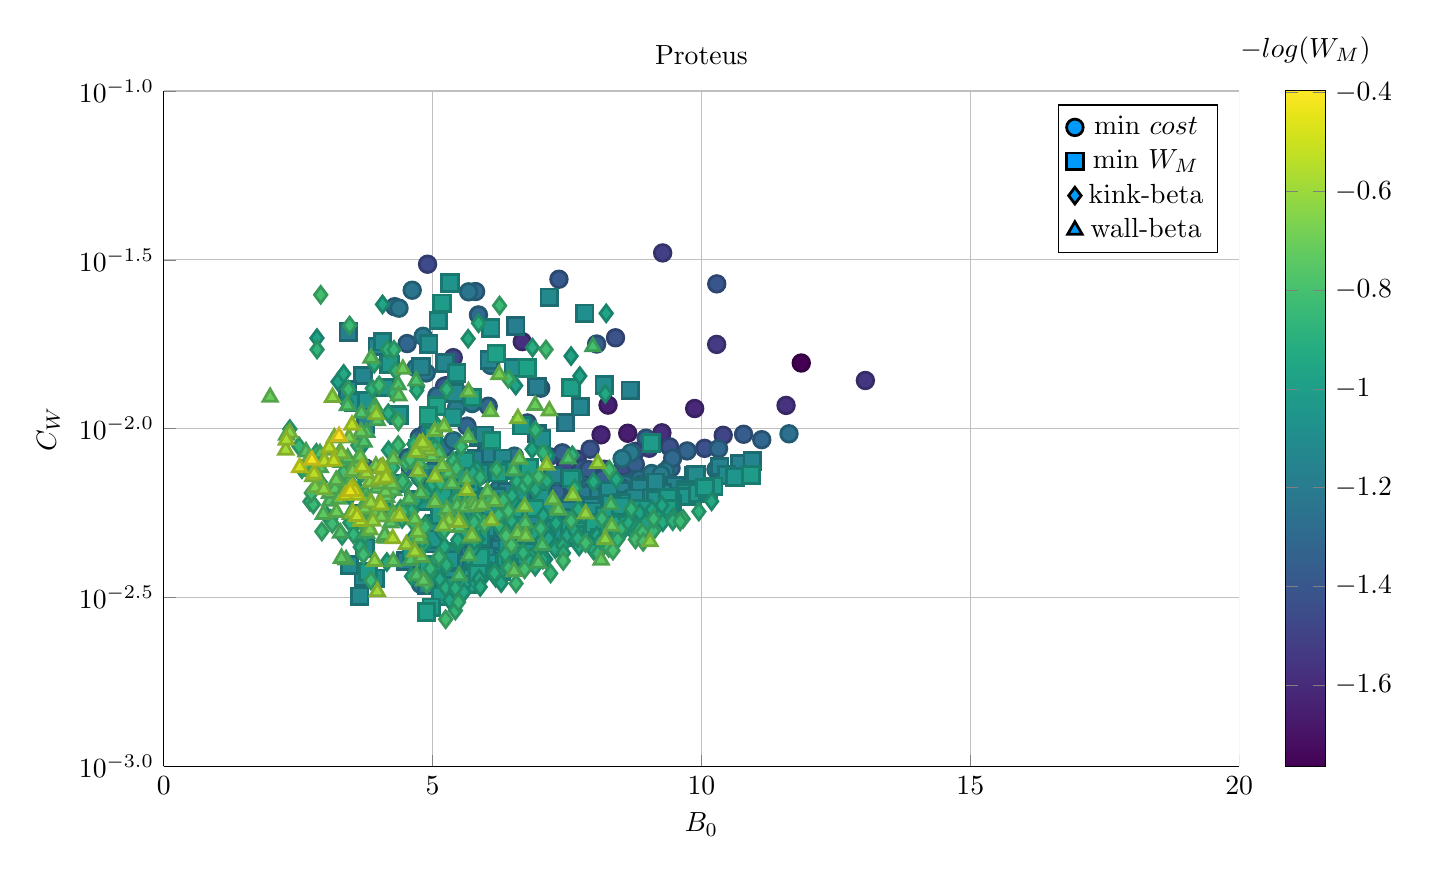
\begin{tikzpicture}[]
\begin{axis}[colorbar = {true}, height = {101.6mm}, ylabel = {${C}_{W}$}, title = {Proteus}, xmin = {0.0}, xmax = {20.0}, ymax = {0.1}, ymode = {log}, xlabel = {${B}_{0}$}, {unbounded coords=jump, scaled x ticks = false, xticklabel style={rotate = 0}, xmajorgrids = true, xtick = {0.0,5.0,10.0,15.0,20.0}, xticklabels = {0,5,10,15,20}, xtick align = inside, axis lines* = left, scaled y ticks = false, yticklabel style={rotate = 0}, log basis y=10, ymajorgrids = true, ytick = {0.001,0.0031622776601683794,0.01,0.03162277660168379,0.1}, yticklabels = {$10^{-3.0}$,$10^{-2.5}$,$10^{-2.0}$,$10^{-1.5}$,$10^{-1.0}$}, ytick align = inside, axis lines* = left,     xshift = 0.0mm,
    yshift = 0.0mm,
    axis background/.style={fill={rgb,1:red,1.00000000;green,1.00000000;blue,1.00000000}}
, colormap={plots}{rgb=(0.26700400,0.00487400,0.32941500), rgb=(0.27794100,0.05632400,0.38119100), rgb=(0.28291000,0.10539300,0.42690200), rgb=(0.28229000,0.14591200,0.46151000), rgb=(0.27619400,0.19007400,0.49300100), rgb=(0.26514500,0.23295600,0.51659900), rgb=(0.25042500,0.27429000,0.53310300), rgb=(0.23360300,0.31382800,0.54391400), rgb=(0.21813000,0.34743200,0.55003800), rgb=(0.20123900,0.38367000,0.55429400), rgb=(0.18555600,0.41857000,0.55675300), rgb=(0.17117600,0.45253000,0.55796500), rgb=(0.15772900,0.48593200,0.55801300), rgb=(0.14618000,0.51541300,0.55682300), rgb=(0.13374300,0.54853500,0.55354100), rgb=(0.12346300,0.58168700,0.54744500), rgb=(0.11948300,0.61481700,0.53769200), rgb=(0.12632600,0.64410700,0.52531100), rgb=(0.15014800,0.67663100,0.50658900), rgb=(0.19109000,0.70836600,0.48228400), rgb=(0.24607000,0.73891000,0.45202400), rgb=(0.31192500,0.76782200,0.41558600), rgb=(0.37777900,0.79178100,0.37793900), rgb=(0.45867400,0.81636300,0.32972700), rgb=(0.54552400,0.83803900,0.27562600), rgb=(0.63690200,0.85654200,0.21662000), rgb=(0.73088900,0.87191600,0.15602900), rgb=(0.81457600,0.88339300,0.11034700), rgb=(0.90631100,0.89485500,0.09812500), rgb=(0.99324800,0.90615700,0.14393600)}, colorbar style={title=$-log( W_M )$}}, ymin = {0.001}, width = {152.4mm}]\addplot+[scatter, scatter src=explicit, only marks = {true}, color = {rgb,1:red,0.00000000;green,0.60560316;blue,0.97868012},
draw opacity=1,
line width=0,
solid,mark = *,
mark size = 3.0,
mark options = {
    color = {rgb,1:red,0.00000000;green,0.00000000;blue,0.00000000}, draw opacity = 1.0,
    fill = {rgb,1:red,0.00000000;green,0.60560316;blue,0.97868012}, fill opacity = 1,
    line width = 1,
    rotate = 0,
    solid
}] coordinates {
(11.855851167264671, 0.015650867313707448) [-1.7651507846396934]
(8.62894306410229, 0.009694646552347688) [-1.652530796858066]
(8.262669569295957, 0.011744038729478485) [-1.647000146345283]
(8.132345586482765, 0.009590177278586947) [-1.6184546481250472]
(9.87352129314419, 0.011474300333025303) [-1.6124908438767973]
(9.26466071494926, 0.00972401084478665) [-1.5828949402967583]
(6.667811597046653, 0.018106858351787505) [-1.577618500437912]
(11.573395463568893, 0.011719738653164523) [-1.56873554690934]
(5.264528343635174, 0.013419897432724169) [-1.5599002750009094]
(13.048135395345042, 0.013892471464509717) [-1.5518482038436605]
(10.282796584070674, 0.017767343192357253) [-1.5302287668791192]
(9.278542294221232, 0.033146306422516245) [-1.5115301730224102]
(7.5044360623009565, 0.007510212646674021) [-1.5013825191439996]
(9.02784009554164, 0.008751202105526691) [-1.4958902811815062]
(8.710683108208965, 0.00816949735167802) [-1.4892617900728689]
(7.687377168804008, 0.008118078139228204) [-1.4884348201277007]
(10.404534949568816, 0.009559158760396884) [-1.4866425610729714]
(5.384524713145202, 0.01623184139531336) [-1.4835478223239928]
(7.472857057569771, 0.007837831837729894) [-1.4780728724015184]
(4.906484287411937, 0.03069401611625924) [-1.4650031348255397]
(7.111580297007043, 0.006765803188842749) [-1.4601242927308113]
(8.773685022223647, 0.008568870415676909) [-1.453691298071198]
(8.545510256202396, 0.007723927816166263) [-1.4489094778079963]
(7.070436548811644, 0.006162431971740805) [-1.432973868001932]
(6.884154096232421, 0.006329451983138475) [-1.4325147285303634]
(9.405921329983288, 0.008839617844718544) [-1.4268866569895065]
(10.057985274469397, 0.008744700190770928) [-1.4268347679685771]
(8.401821549997786, 0.018590297650719324) [-1.4237681445033143]
(8.189937032371649, 0.007587250291191641) [-1.4234658725845162]
(8.234578254729767, 0.007390656211515189) [-1.4109108269606008]
(7.92991212471289, 0.008694085637837138) [-1.4079262096010774]
(6.59839258184741, 0.00634066157530613) [-1.407330123320285]
(10.284931156770094, 0.026840973164111593) [-1.3996791570309395]
(7.3137838143058795, 0.007040053838733538) [-1.3974870797438]
(5.221820332167986, 0.013359280479800206) [-1.3946269662443698]
(7.785957307166937, 0.007634837530984513) [-1.3905305073664083]
(7.069469201177765, 0.006488653571629467) [-1.3895960301339119]
(6.200523563918331, 0.00554611680879456) [-1.381931002288656]
(7.340133149046422, 0.00695131625200887) [-1.3818272949203658]
(7.349866215424601, 0.027704627448181397) [-1.3812563757949996]
(7.351199097200025, 0.00681167564679013) [-1.379699079550137]
(8.120289345307025, 0.006715817539753603) [-1.376650573885692]
(7.90274300232169, 0.00757067906104037) [-1.3758581110553065]
(7.565484576443418, 0.006499559071472007) [-1.375220700855124]
(7.688718501611012, 0.00646934556613389) [-1.3742348635950123]
(7.005633077388933, 0.0063267927368600325) [-1.3713423550361032]
(7.166534585210968, 0.008267480512087599) [-1.370057699317172]
(5.695615872659735, 0.004988896324536347) [-1.3686239973313072]
(6.620180775083285, 0.005540386026064644) [-1.3680076928767484]
(5.712356159098289, 0.005024205798518008) [-1.3672266212882762]
(10.783439028923059, 0.009628839399324697) [-1.3667105305870977]
(6.000471468140266, 0.0050592629231849704) [-1.3651176317240314]
(8.050752136473724, 0.017814080806893125) [-1.3612722200713383]
(8.77043990632116, 0.007840171434328094) [-1.360737823431438]
(7.010340303297389, 0.013182987051350502) [-1.3596008789905631]
(7.295294539644262, 0.006730765435871485) [-1.3568098625263256]
(6.641599582701438, 0.005632641769207446) [-1.3562925407270994]
(6.645748730966029, 0.005613911931897123) [-1.3540300242042478]
(6.054699810485283, 0.005176189759381431) [-1.3527684291391184]
(9.401252816575663, 0.007678792615766904) [-1.3513432280511455]
(5.581708167132495, 0.006888425944911811) [-1.3508742741062625]
(7.803535098905909, 0.006674090356682625) [-1.348444904526092]
(6.76411548346407, 0.010402669872398145) [-1.3482429808137002]
(8.969455503638764, 0.009376571407375644) [-1.3481015746033576]
(5.634510628688515, 0.012583797530216616) [-1.34746159692277]
(8.156032796881272, 0.007115527316776566) [-1.3450418873098828]
(7.056939291922313, 0.006464286011476574) [-1.3449397649071608]
(7.240799475525162, 0.006186516144095541) [-1.344834769873685]
(6.571134452649435, 0.0053864817732829605) [-1.3436955024234147]
(7.4120702527384665, 0.00848434463520388) [-1.3426163725681677]
(5.934011898969639, 0.004938310227983135) [-1.3374912582230194]
(7.37766442956072, 0.006636608478826529) [-1.335539302100867]
(5.026669706190863, 0.007606581585076429) [-1.3352915983538123]
(6.825792187162438, 0.006029019944814239) [-1.331337874103357]
(9.732916904654346, 0.008594819258321628) [-1.3310780697195672]
(5.698038434377145, 0.004728216221281147) [-1.3292068036291638]
(6.854283769326888, 0.005953363383436291) [-1.32828646244698]
(4.7527705925878685, 0.009441137210103956) [-1.3280975618898123]
(6.452485475407575, 0.005079524630506098) [-1.3278697867431468]
(6.6282734062471, 0.005749625528658903) [-1.327757292865828]
(7.362442088263758, 0.006249734903697681) [-1.3253106415861637]
(6.357926345811093, 0.005155209960292018) [-1.3237407060184172]
(9.434691757978365, 0.007650804529712704) [-1.3217246458754282]
(5.945683748997239, 0.004926318213851794) [-1.319376268743699]
(5.716699212704698, 0.004774448071559269) [-1.3182101821558738]
(7.9999703999657505, 0.0066268624262571275) [-1.31770129332637]
(4.526018058829261, 0.017867829271260238) [-1.3171626271127284]
(7.307142270921693, 0.006479743346210051) [-1.3144438328362922]
(5.64022055353738, 0.010177994071422254) [-1.314397397461996]
(11.121291715489328, 0.009279261565995508) [-1.3134452963620502]
(6.890660641840135, 0.005896178522672516) [-1.3126768401499638]
(5.8496112618323926, 0.007223214696135702) [-1.3123916957087167]
(3.755618871416242, 0.007643344629724278) [-1.3117090270675453]
(6.965828665871357, 0.0062843154751196315) [-1.3112976001573549]
(7.132942553696917, 0.006316305209750007) [-1.3102933400586538]
(6.034623082086722, 0.011655743235665423) [-1.3084666426112759]
(9.464190150712176, 0.008181643780093392) [-1.3081739820914746]
(6.735484315816856, 0.005920113041607297) [-1.3081169022767745]
(6.329532230716051, 0.005266304291939928) [-1.3075986397555424]
(6.949512174456946, 0.0056632699287416785) [-1.3038897119548887]
(5.7123865302563095, 0.004515583648974614) [-1.3034916079905217]
(4.588431546307119, 0.00762405310841983) [-1.301506470226052]
(5.8529754306366, 0.021723513711501174) [-1.2978787946122285]
(6.763583440942078, 0.005860560202229156) [-1.297460949292816]
(5.79974352272628, 0.02547444831481485) [-1.2953226778576867]
(4.294506467374343, 0.022974551007964673) [-1.2951062787178942]
(10.317711969577175, 0.008727794605170999) [-1.2946978796261759]
(7.030442720189729, 0.00606442154900928) [-1.293243062455323]
(6.3155245633398005, 0.00478216163852665) [-1.2916316854649297]
(5.594153930448576, 0.004505685536187866) [-1.291573412415986]
(7.0608047385200905, 0.006201757851874389) [-1.2910367642815292]
(8.746159160738731, 0.007056272547770033) [-1.2894268757747884]
(5.790961836119614, 0.004812007322004063) [-1.2891780169645117]
(7.13931972393237, 0.005900795309436559) [-1.2883016772579983]
(5.642350264315365, 0.004575860387174974) [-1.2877120777365891]
(5.500511487756749, 0.007501625869556503) [-1.2825608117529994]
(5.1870060839860015, 0.004048206616482656) [-1.2803416949249293]
(5.0793762257146975, 0.012501014524680899) [-1.2790944723531177]
(4.900710067477188, 0.009849033693022476) [-1.2789599032268324]
(5.416336002756713, 0.004266328381972482) [-1.278637308935949]
(7.047880217226236, 0.00602317781329061) [-1.2752962713941192]
(4.537987048593646, 0.008202673797589401) [-1.2724318730764337]
(6.7947527911354095, 0.005313590913225172) [-1.26778944603233]
(7.547856502776895, 0.005746237915345085) [-1.2652894696394015]
(8.337373800803634, 0.0063394092295352205) [-1.263844406219344]
(5.839234828237175, 0.004670640784960837) [-1.2622412045786418]
(6.307588148065544, 0.005025369604276285) [-1.2622057750392766]
(6.369182324037021, 0.004715175023029078) [-1.2568407944078956]
(7.25221896281004, 0.005515822538041083) [-1.2564369672634057]
(5.207422458409709, 0.008763742702873716) [-1.255580803936347]
(8.846964102011665, 0.007090160917314494) [-1.2542825781236586]
(11.62801313878366, 0.009658252430988482) [-1.253606675738751]
(6.586437041421525, 0.005078101074449218) [-1.2533258835374417]
(5.896819232149536, 0.004668333949768413) [-1.252740293490489]
(7.218625057420257, 0.005623439530060779) [-1.2512906609771755]
(4.770007649977626, 0.007192663750971734) [-1.2505906665339703]
(6.391248250395476, 0.004753912504004936) [-1.2505667349102745]
(6.722228809625436, 0.00547669175115548) [-1.2505409706978425]
(5.9975644347104575, 0.008585550973626429) [-1.2504311283223648]
(6.220483255591395, 0.00536142422310656) [-1.2495193060816674]
(7.131398255569569, 0.005891517799670805) [-1.2472203996667584]
(4.620896334693883, 0.025703839631456088) [-1.246340221801285]
(5.634708074324937, 0.004426672964739238) [-1.246337044553182]
(6.0053836269885, 0.004733745531528537) [-1.2444533586241864]
(6.122472771064873, 0.004373459187272198) [-1.2410504069560844]
(4.881468969197191, 0.014622918962551527) [-1.2404616678069278]
(5.669873863181108, 0.025422666134658947) [-1.2402101811954278]
(9.159921449108527, 0.00699405114862055) [-1.2399625556579728]
(6.619988989498716, 0.005459593535350185) [-1.2395775558220574]
(4.0721743569002395, 0.006780135026174841) [-1.238968027160994]
(8.487125648729805, 0.006381273355008305) [-1.2381935518916032]
(5.785136288326493, 0.005454977773134567) [-1.2372164242860222]
(7.805870043590986, 0.006162937475975255) [-1.2359322527835273]
(6.521775930847536, 0.008295248979234676) [-1.2345953253761524]
(7.299795216034374, 0.005661235915534237) [-1.2333782101635051]
(6.654376116038794, 0.005116145429327062) [-1.2329256482335589]
(8.586321868785943, 0.0068738253515159406) [-1.2318041138227]
(5.871716076416853, 0.007759607253139788) [-1.2286780396839752]
(5.525881431830733, 0.004270512991179436) [-1.225800447150557]
(4.37566370657649, 0.022744869820021597) [-1.2237626122718148]
(5.386416012885563, 0.009221148903357415) [-1.2192315569877235]
(5.735606858683557, 0.011868028475244749) [-1.2191811590789894]
(8.68706974133124, 0.008481483201532794) [-1.2185680785343938]
(8.63032181590475, 0.00622802822970762) [-1.2179132583990178]
(8.508158073563377, 0.006703260233628488) [-1.2171472173843672]
(7.953691408978824, 0.00633213628058925) [-1.2167448502658762]
(6.081331959057098, 0.015392818825938645) [-1.2162995250149307]
(5.225401290559421, 0.003872910530196867) [-1.215703789534109]
(5.988978974443945, 0.004720977485089404) [-1.2156312790675603]
(9.073087462786646, 0.00736963569440644) [-1.2145283350978044]
(7.217725198328268, 0.005383150867826381) [-1.214317974252912]
(5.536577745729214, 0.004178935326843822) [-1.2138536176262873]
(4.776559777248383, 0.0034641548226198885) [-1.2119360055173332]
(5.211688187540344, 0.0038140534914709043) [-1.2104347246988538]
(10.269380266980404, 0.007570292211977012) [-1.2084631186053005]
(6.918845939903695, 0.0052385995930077645) [-1.2083264519217767]
(7.0692693982238906, 0.005083028024589718) [-1.2073346872626274]
(5.874112036399968, 0.004039129704078142) [-1.2071975929322125]
(4.690082401892927, 0.01513911751066285) [-1.2067840670536927]
(7.861161945792819, 0.006395373245847939) [-1.206736577191552]
(9.326423266814658, 0.007483645463069493) [-1.2065799786199445]
(8.029413669351802, 0.005698374888186277) [-1.203843641047789]
(6.959732144718079, 0.005550896360654382) [-1.203724365314369]
(6.960477287319412, 0.005010777712400389) [-1.2024406864855146]
(7.654476699386534, 0.007157947201399507) [-1.2021169810907544]
(4.823547237227045, 0.01877759730610099) [-1.2015933815507112]
(6.062862639710857, 0.004489267037355289) [-1.2014423796656961]
(8.999102001729389, 0.006374667856956503) [-1.2011965112492808]
(7.2717504340335415, 0.00572395742880883) [-1.2005427289121806]
(6.227413325881237, 0.0066192080125215165) [-1.1994215784439877]
(9.247503176233229, 0.007316062816603203) [-1.1975084180232178]
(5.443249511926066, 0.011502671870448664) [-1.1972619972446426]
(6.742357647461489, 0.005266662336518346) [-1.1967371969067386]
(5.926964832086266, 0.004368135902166705) [-1.1965134818457024]
(8.524769827029726, 0.008154332104698897) [-1.196084536648355]
(8.867575034400405, 0.006843978332329513) [-1.1943424204563022]
(6.457339766119646, 0.005029914775543452) [-1.1908054127888088]
};
\addlegendentry{min $cost$}
\addlegendentry{min $W_M$}
\addlegendentry{kink-beta}
\addlegendentry{wall-beta}
\addplot+[scatter, scatter src=explicit, only marks = {true}, color = {rgb,1:red,0.00000000;green,0.60560316;blue,0.97868012},
draw opacity=1,
line width=0,
solid,mark = square*,
mark size = 3.0,
mark options = {
    color = {rgb,1:red,0.00000000;green,0.00000000;blue,0.00000000}, draw opacity = 1.0,
    fill = {rgb,1:red,0.00000000;green,0.60560316;blue,0.97868012}, fill opacity = 1,
    line width = 1,
    rotate = 0,
    solid
}] coordinates {
(7.4724590738720655, 0.010422279639263054) [-1.1890033537880158]
(6.938996985119089, 0.009658294464102987) [-1.1883675827161198]
(6.9393893920794385, 0.013313745665171912) [-1.1879538738656286]
(6.377850385556073, 0.006487414571263668) [-1.1878029685724296]
(6.547487324963764, 0.020145877705477357) [-1.186260879134981]
(8.029613686159495, 0.005801884747670386) [-1.1859242026174677]
(5.6874025972941205, 0.004217349677698315) [-1.183889066210908]
(7.827309596895398, 0.0058827996938258294) [-1.1830291222504283]
(5.8219713598117036, 0.008160599297710009) [-1.1826268505607591]
(6.946718058585209, 0.004857174007518612) [-1.182365307189366]
(3.434094114791118, 0.01935279381255584) [-1.1822251925764147]
(6.23809783755075, 0.00447855648592392) [-1.1813612663460882]
(5.88781791976068, 0.00428725320402622) [-1.1785285195809967]
(4.505121226933233, 0.004053651772674214) [-1.1775655951090325]
(6.553162158329651, 0.005121496915389368) [-1.17705398157876]
(5.8303432949169745, 0.005890819973806921) [-1.1767452937515073]
(8.807822926389145, 0.006104718148251412) [-1.1766083315756861]
(4.18691738643155, 0.01556268699280997) [-1.173888237216638]
(7.55203601905607, 0.005882961839613334) [-1.1734465174435744]
(5.819836385827624, 0.005961179911412564) [-1.1729466514857931]
(9.116693027577789, 0.006287276174883399) [-1.172839252676928]
(3.659189590525744, 0.005599267038542826) [-1.1727769211527406]
(7.004035835152084, 0.005070632392189801) [-1.1727372361954858]
(4.897086463141796, 0.003434292526080427) [-1.1726542785062386]
(8.087708955601924, 0.0062657093568900535) [-1.1703764252048678]
(6.7024429891400565, 0.004942047034638912) [-1.1699166462753263]
(5.893015258208656, 0.004183590560340062) [-1.1681831393061217]
(7.479710666339309, 0.005170881199231806) [-1.1671080842733117]
(9.508375514310952, 0.006777996547666784) [-1.1655606692177785]
(6.075560203652315, 0.008402469668507205) [-1.165303541813206]
(6.61932998550545, 0.004666935296152095) [-1.1643973078802388]
(6.286558265163782, 0.004663766235492665) [-1.1632535008384055]
(5.050068824721165, 0.004566940606242733) [-1.1631989573193973]
(7.688714523679582, 0.0054331000812183365) [-1.1630392685982025]
(8.505800422917172, 0.006544368204474158) [-1.1625753891662707]
(8.975209897762664, 0.006511116933487475) [-1.1617936783337066]
(8.380983437312786, 0.006126048639979384) [-1.159367616011031]
(8.67470730810651, 0.012995381528200805) [-1.1593260324319568]
(5.960621269295445, 0.004013416769217783) [-1.1592024857112633]
(6.282535161243701, 0.004530529794416821) [-1.1590403977294572]
(10.712436821713085, 0.007867971330715704) [-1.1589428109110296]
(7.099415207654768, 0.005330271588661515) [-1.158451320077056]
(10.3395352744249, 0.007724720119696045) [-1.157468772898154]
(6.536306152444655, 0.004436262085616985) [-1.1570637161067505]
(9.855000808062698, 0.007249642226094706) [-1.1563966451418943]
(5.856384724795581, 0.009420901412013665) [-1.1561531921827275]
(7.454679880823048, 0.0057898611640113395) [-1.1538328200442942]
(5.14753239685863, 0.007237376261288284) [-1.1525173430901554]
(6.856563325018079, 0.004881019954742076) [-1.1522162283529644]
(7.618840457764884, 0.0059379940430840635) [-1.151968932860403]
(8.398440991699191, 0.0061407721476487214) [-1.1511586507355254]
(4.781165601129724, 0.015255960449664327) [-1.1509834966159156]
(6.247011281135245, 0.004419080970160178) [-1.1503660387736743]
(3.7553680100049234, 0.01032617135589161) [-1.1500086948877408]
(5.5152996897670015, 0.004014883666259908) [-1.1494080253790357]
(7.800728278542519, 0.005291422749753008) [-1.1493093072503229]
(6.054088477025007, 0.01598351560152435) [-1.1489823622220707]
(5.411295562966824, 0.003915099463846501) [-1.1484511044037433]
(7.052045109627868, 0.005020529922825154) [-1.1483999797493492]
(5.28488049549897, 0.0034947010100993764) [-1.147064765638366]
(7.62011089503286, 0.005859550653426385) [-1.1465028274549764]
(7.468210164743146, 0.005641165149475234) [-1.144883586902141]
(5.595946792423691, 0.007176119328254024) [-1.144368544047569]
(10.943656185786155, 0.00802165691682325) [-1.1435280806157744]
(7.908061023064291, 0.005447269817044685) [-1.1433393449411435]
(8.854582349908517, 0.006668732693209443) [-1.143332108158641]
(6.549837080949351, 0.004886014774808058) [-1.143184585873657]
(3.9729755898485215, 0.017515494611674454) [-1.1428249654095861]
(3.703954177548893, 0.014377117697389604) [-1.1427984862828113]
(3.4213090828497417, 0.013005276311642224) [-1.142397010267489]
(6.02709699747974, 0.005929095379259443) [-1.1423708774410877]
(5.231750077921478, 0.01565086593371781) [-1.1422424769576425]
(7.2349136535832095, 0.007266091038483963) [-1.140012696356206]
(7.647205004097057, 0.005840600330748377) [-1.1399465227440013]
(6.532016233135844, 0.00480284773560221) [-1.1387943392990294]
(7.523885505796154, 0.005752426766742318) [-1.1382802201938975]
(7.750130276532692, 0.011612930840038163) [-1.1380314198362265]
(9.276469763067444, 0.006446360072583165) [-1.137892443914052]
(5.952941013085345, 0.009562541252399106) [-1.1311113631375915]
(7.951426521304668, 0.005743536904522906) [-1.1302954325651586]
(5.952653119927932, 0.0041760314888273755) [-1.1295543261638465]
(8.253192497448524, 0.006161648966500728) [-1.129462828049983]
(5.512192429439468, 0.00369116854025651) [-1.1277963061708562]
(6.180741676638315, 0.006278926396423389) [-1.126807171194116]
(6.608627477861355, 0.004487529275565533) [-1.1267021554022474]
(9.14457555501132, 0.006938744439971839) [-1.1265761162904897]
(5.310301950330671, 0.004304336836767321) [-1.1261385034152473]
(7.969320198807478, 0.005917258047258142) [-1.1260458936236624]
(7.954215183655014, 0.005885263457738176) [-1.1250537668582923]
(6.771595293849517, 0.005616858230043609) [-1.124511019242948]
(6.641944516873176, 0.004843731890681865) [-1.1236988869720232]
(6.896134858333351, 0.005173923137495115) [-1.1235064786985465]
(3.7132325707792995, 0.003624821435760545) [-1.1232730371267585]
(4.936839162331792, 0.007429853985811719) [-1.1231293548483412]
(6.555316024199809, 0.005231942783984398) [-1.1209978185544383]
(6.304604592673814, 0.008169617815892689) [-1.1196911148335087]
(8.737416781995437, 0.0061580609115664325) [-1.1194748634113345]
(6.123815672401932, 0.004188882178419093) [-1.119418152841014]
(8.324353852438948, 0.005791769416647159) [-1.1191123923650526]
(6.830685941792606, 0.004931972266091366) [-1.1181736482095217]
(8.279157421008941, 0.005611347227289511) [-1.1176702646643628]
(7.172394160745635, 0.024480989089009208) [-1.1175403888423328]
(6.753756430979739, 0.004518885765871233) [-1.1174827013795072]
(8.76524294869496, 0.0062233325455323925) [-1.1174414411464733]
(5.952289891041446, 0.006299808378708293) [-1.1171134960728113]
(6.523754565443294, 0.004568184715721437) [-1.1171111976535804]
(5.4096290381473375, 0.012757776435747556) [-1.1168806186241906]
(9.896916686410892, 0.007305420869085463) [-1.1160945644374545]
(8.286804128590813, 0.005340773800773009) [-1.1139896885893594]
(5.399012890266871, 0.0036233885329560954) [-1.1123768792739945]
(8.296167355721272, 0.005311493039288053) [-1.1112153482766423]
(6.778775360762903, 0.0045000578497955725) [-1.1111283014916062]
(3.642453456441478, 0.003188662256079057) [-1.1108869662710774]
(6.918579935305505, 0.004842654136629077) [-1.1089922492653659]
(6.5071710234613676, 0.00452032863173795) [-1.108391782497311]
(7.258592477367294, 0.00535669926333167) [-1.1082929384878708]
(6.6776055936353265, 0.004745534590751309) [-1.1074346113685616]
(5.3226296796509205, 0.004323464728471098) [-1.1074227437950106]
(10.46985584146923, 0.007293078759243216) [-1.1069130893453907]
(3.4547855533452156, 0.003945456212149148) [-1.106325178133445]
(7.57975455174028, 0.004982808461571556) [-1.1060035644106432]
(5.06842585608741, 0.0052409052861536465) [-1.1038776732161713]
(5.698043204630489, 0.0065314531396132094) [-1.10351060592976]
(7.734654274692709, 0.005173060010686301) [-1.1022315889718237]
(6.228402773452205, 0.005951424789746293) [-1.1016702257969113]
(5.288893434740895, 0.007437806150470808) [-1.100448826904311]
(7.254453932047169, 0.005288339533793414) [-1.0998565094908217]
(6.807046489565401, 0.004337170224988449) [-1.0995498480529582]
(8.496667761878552, 0.005750254423520601) [-1.0992970719713648]
(6.506723144546308, 0.004423364554484401) [-1.0987351440216522]
(8.273277101596172, 0.006535275113176343) [-1.0983869460625248]
(7.024499917691516, 0.006822630998366228) [-1.0977261444257258]
(4.929559505548113, 0.017828562633364364) [-1.0969882385788774]
(6.546519891753608, 0.004407786879742766) [-1.096807077081938]
(6.299458688060015, 0.0041501216036249275) [-1.0962033310727437]
(5.917588131126826, 0.003972749736578854) [-1.0948458082881816]
(6.5027787367036485, 0.015155543307471772) [-1.093965318294314]
(8.191093731826841, 0.013471957430229371) [-1.093275686079877]
(5.765417917352738, 0.003923510470624812) [-1.0931318196649105]
(4.067683728143941, 0.01811006730780237) [-1.0926393639694263]
(5.643295069658257, 0.005671433069083637) [-1.09199330517098]
(5.33448260992027, 0.0035546432563184145) [-1.0916603258728452]
(5.996010919360583, 0.005082501155756355) [-1.091508438458307]
(6.130249778803564, 0.003922207642532424) [-1.0911853630489914]
(5.152309500808404, 0.007129588907950501) [-1.0896526200520398]
(6.613976143688219, 0.004468466025444819) [-1.088663441639713]
(7.828710312153846, 0.021949864805969728) [-1.0877780715734315]
(7.029871400370792, 0.009322832924906896) [-1.0870739196827126]
(6.6598420793586, 0.004672088916974179) [-1.0855818982110972]
(6.33097870945106, 0.004039319528471343) [-1.0844715994400023]
(7.702268833143657, 0.0053439960085053) [-1.0842780595786392]
(6.084754710909704, 0.005760793758021615) [-1.084266572782003]
(7.98999393987453, 0.00569380985136289) [-1.0839928767281124]
(5.068992476376386, 0.0039349920083461085) [-1.0828594792618813]
(9.086048642306793, 0.0062405207423892875) [-1.082853352734588]
(7.44906676523106, 0.0054577800846403015) [-1.0824719035597]
(5.375575122544495, 0.0035809652689903063) [-1.0824709528228211]
(7.386984140765724, 0.005148297391297789) [-1.0814366033908964]
(9.702271536107535, 0.006582162000449632) [-1.0809878234039578]
(9.614854186704672, 0.006301853688415234) [-1.0808972954130593]
(4.645688111866446, 0.006161790226168522) [-1.0797863646031054]
(3.927334262139488, 0.0036086053477567665) [-1.079163153355685]
(6.963971610592974, 0.004793357206410555) [-1.0780309855478056]
(8.244956752748422, 0.0054298508521766365) [-1.076806285491668]
(5.769697532800943, 0.00604411217248383) [-1.0765985094568509]
(7.283344319549832, 0.004828662165485411) [-1.0760641298404754]
(5.392578394594405, 0.005661819547798889) [-1.0757730303287785]
(3.7434225317786316, 0.00443044659495794) [-1.0744056068515366]
(7.7252366425534715, 0.005467468655559742) [-1.073726482715373]
(8.506016241294386, 0.006046667097602973) [-1.072815333291583]
(5.722077224788854, 0.006315687038558954) [-1.0718638391063322]
(3.5290681872248832, 0.011989877345034696) [-1.0710072465261937]
(5.408389828424612, 0.006287200186056995) [-1.0706716976099708]
(5.880603880610476, 0.00739594343637032) [-1.069478881808043]
(3.770984054785403, 0.012080600310741674) [-1.0679830462657767]
(9.144669371614333, 0.006138341400017388) [-1.0670572282884458]
(5.3325423351198395, 0.004085658341340117) [-1.0667391835901658]
(8.316799187366927, 0.006004004929014098) [-1.066302608545655]
(6.389619437625667, 0.004440975162005993) [-1.064104157833971]
(5.324355765249537, 0.026972932068461592) [-1.0640878812065675]
(6.511622532652898, 0.004395996587917252) [-1.0635820925869255]
(6.911249511094287, 0.004423420241739423) [-1.062988318250961]
(7.502962627592097, 0.00480727122317776) [-1.0628036997189863]
(5.469724443246719, 0.0034131330547271113) [-1.062700357913494]
(5.706475165604361, 0.0036974585830479817) [-1.0626514373993834]
(7.276669037534987, 0.004776499853086686) [-1.0610739421064752]
(6.526975357350624, 0.004144297606935685) [-1.0588352037418618]
(5.105089902831069, 0.0209014980088616) [-1.0585986545827941]
(4.374531653432859, 0.010988948677442597) [-1.057135771526312]
(4.122473679442906, 0.013241941603829825) [-1.056315661795303]
(6.078673477412938, 0.019862106250452566) [-1.0562734967702754]
(7.427558910001991, 0.004858658731965693) [-1.0561257856094448]
(7.01015270925273, 0.006223828461257365) [-1.0559814704124602]
(5.014809023336614, 0.004706089102701761) [-1.0555859489072712]
(6.029077134394886, 0.003994614402213268) [-1.0549803415205259]
(9.718000396033032, 0.006463993798881436) [-1.0545713902023608]
(5.896086527792721, 0.0038990516235787613) [-1.054205756099488]
(10.62632239203378, 0.007195479612398366) [-1.0536290024409787]
(9.830251746280974, 0.006286763322784177) [-1.0533216125601341]
(5.653429182632709, 0.004822724612666477) [-1.0529307720930816]
(7.148582094551358, 0.005656264568736301) [-1.0525850668019536]
(9.721783343528084, 0.006295530789348686) [-1.052552508886994]
(6.4747129291886205, 0.007550888758433211) [-1.0509835312174363]
(7.5553171987129115, 0.004904482654727138) [-1.0508250621973283]
(5.689433662550519, 0.006571304536184572) [-1.050680345054969]
(6.819358408267933, 0.004560195418506711) [-1.0506245233592775]
(5.372500908480495, 0.01080264515897382) [-1.0505217359121972]
(9.464104357867244, 0.00597835329976134) [-1.049317623712287]
(9.421645636318559, 0.00605275476812188) [-1.0490747591885061]
(6.83923495211403, 0.004511808104116367) [-1.0489907539423449]
(7.595014509377157, 0.0049153150140211965) [-1.0478434867034416]
(6.9492853284169565, 0.004616652674773231) [-1.0473758850488442]
(6.631954997333512, 0.006447737760929581) [-1.046767629611379]
(4.836574702453568, 0.006114416229637186) [-1.0460742739305466]
(5.447392742867525, 0.01461141466329314) [-1.0428746875530057]
(5.278008805745069, 0.0034297894059699906) [-1.0409932776852704]
(6.869290933859089, 0.004324846597058025) [-1.040720375777512]
(4.388359570069462, 0.0068957525832947) [-1.0400494553390642]
(7.730136216039545, 0.0047742837106654985) [-1.03963800286999]
(5.097390647393597, 0.0070972253563865) [-1.0394862991533038]
(5.705197239891871, 0.006107051538135721) [-1.0391370640013136]
(4.211114439903267, 0.015503036624972183) [-1.038354289214968]
(9.925180494788561, 0.006445735380428859) [-1.0380750082543837]
(8.392824243874195, 0.005205902574339689) [-1.0370263081612092]
(7.973811270774484, 0.005283195240312258) [-1.0365321066837632]
(8.49921904371083, 0.005892181423629392) [-1.0364145571368009]
(6.655649338522086, 0.010214094301379546) [-1.0358730287795153]
(6.272206414918943, 0.003781581128188247) [-1.0352797650690977]
(9.40142074331525, 0.0061316127141858145) [-1.0352425491421158]
(4.6061758509773245, 0.004345014451914255) [-1.0335536367675167]
(5.764426452876033, 0.00415632052734694) [-1.0319535365225938]
(9.372888478292797, 0.006253917955260214) [-1.031638330454266]
(5.729013310777877, 0.003613822408322808) [-1.0316283345953763]
(5.883030813164119, 0.00478160347928963) [-1.0312630056422283]
(6.556479558238363, 0.004326998549376461) [-1.030801418278412]
(6.395724956994062, 0.006039359373565179) [-1.0301227610636083]
(5.139256557257989, 0.005550817437725965) [-1.029015666765989]
(10.123332193763748, 0.006583295742064639) [-1.0288573869793878]
(6.568561456688728, 0.004204292638824563) [-1.0245024368116802]
(5.6039086370880105, 0.007145400138218064) [-1.0231385619546913]
(7.648719554707365, 0.004789677204757558) [-1.021449027000752]
(10.226601060349507, 0.00675373673736514) [-1.0213127693885564]
(5.153470412653239, 0.003193542226257652) [-1.0209276741398987]
(7.579001576207003, 0.007121099635585821) [-1.0202684704954939]
(3.8015765702844804, 0.0037708668397859442) [-1.0187837906200732]
(8.894908266877893, 0.005805595496214904) [-1.0179738483919518]
(9.066566182501706, 0.009070154520460257) [-1.0169425110693646]
(8.213444606213486, 0.00501503870041615) [-1.0162045101447212]
(10.062564168396998, 0.00670010251636303) [-1.0149810946438107]
(4.727731778507776, 0.008752580219573484) [-1.014353466976016]
(5.174769297851055, 0.023528952793841592) [-1.0140528730661398]
(8.195915051921629, 0.005527004085356763) [-1.0133093427968076]
(7.054369905297556, 0.004778958682375364) [-1.0128360857902137]
(5.031848935370691, 0.003842216867194081) [-1.0126834015105255]
(10.922140692684003, 0.007300503854095673) [-1.0124869131348806]
(5.915584448350069, 0.0038089628255598917) [-1.0084966915198963]
(5.602678326023923, 0.008048423371546378) [-1.005776006726422]
(7.544600594243294, 0.005136336479510988) [-1.0027757315503723]
(4.977942341177753, 0.0029594317443149176) [-1.002422823826331]
(5.642218938318191, 0.003459304695059543) [-1.0023352556688647]
(8.295019648678474, 0.004988217345842403) [-0.9994656987080655]
(7.070940189155582, 0.004649343635980374) [-0.9991953302395459]
(6.226711465325763, 0.007411548557741582) [-0.9991876183275935]
(6.419292049664728, 0.0038831217844692545) [-0.9971256954762724]
(4.887255844769486, 0.0028654321699102935) [-0.9968293366364798]
(7.7523402111694955, 0.004992975570566671) [-0.9965130838642419]
(5.890289877584987, 0.003830578946172306) [-0.9960911988132904]
(7.574296219984337, 0.013215773066776348) [-0.9953080727443692]
(9.012153601445592, 0.005338097758519931) [-0.994764309342816]
(9.386356586964215, 0.005798704578553127) [-0.9941918143808477]
(6.789856926677994, 0.007661762309327555) [-0.9939974184414383]
(5.741492166499531, 0.012372283627325148) [-0.9936895922796631]
(8.093840230774958, 0.0047417231470052315) [-0.9920762514365737]
(8.423301149042322, 0.005175409039233765) [-0.9891335090238219]
(6.5096125388500665, 0.005799134035216279) [-0.988320863141931]
(6.362065295698958, 0.003975692742134705) [-0.9873980470532571]
(6.898795759334327, 0.005803966541873779) [-0.9872638091155089]
(5.86662772167221, 0.005281651647264406) [-0.9871243344745786]
(5.00980677003057, 0.00954881671016918) [-0.9862026242600886]
(6.0980328290063905, 0.009231911938640338) [-0.9851939256634008]
(8.004532839270633, 0.005233428706224578) [-0.9845137991026185]
(6.760939557779194, 0.015110407509335635) [-0.9844063088607684]
(5.192252043701997, 0.006274740712107015) [-0.9843851675543582]
(6.182612803400956, 0.01666579340898781) [-0.9832677624207663]
(8.112468976523042, 0.004743145828135927) [-0.9823156156623659]
(5.841361480008224, 0.003744148435661381) [-0.9817957805945331]
(7.647006952351862, 0.0048552692105239565) [-0.9817262777133879]
(5.077285700891451, 0.01167873981501713) [-0.980944500204026]
(5.883453787587344, 0.004161496814710868) [-0.9808435285359967]
(4.920420200443467, 0.010903168023481107) [-0.9803069086017846]
(8.471906861597214, 0.005187973951951495) [-0.979926239566149]
(4.915731269106913, 0.0039527765780552285) [-0.9799255860420428]
};
\addlegendentry{min $cost$}
\addlegendentry{min $W_M$}
\addlegendentry{kink-beta}
\addlegendentry{wall-beta}
\addplot+[scatter, scatter src=explicit, only marks = {true}, color = {rgb,1:red,0.00000000;green,0.60560316;blue,0.97868012},
draw opacity=1,
line width=0,
solid,mark = diamond*,
mark size = 3.0,
mark options = {
    color = {rgb,1:red,0.00000000;green,0.00000000;blue,0.00000000}, draw opacity = 1.0,
    fill = {rgb,1:red,0.00000000;green,0.60560316;blue,0.97868012}, fill opacity = 1,
    line width = 1,
    rotate = 0,
    solid
}] coordinates {
(5.163569333804058, 0.0049343734079309275) [-0.9797193514246809]
(7.7377435890937285, 0.014326928101993836) [-0.9793649258547107]
(5.770648171127724, 0.004418560150536774) [-0.9793554194238832]
(4.7261265073999565, 0.007133046942930264) [-0.9793399260652301]
(4.749925847834237, 0.004527202123528333) [-0.9786718824413932]
(3.240965863210715, 0.013777079521683793) [-0.9784247640598123]
(8.408728218761828, 0.005278344797288595) [-0.9784156054323705]
(5.20936895107677, 0.004002965553163199) [-0.9772101816150688]
(6.546367069245276, 0.013418113026562503) [-0.9771245449599791]
(6.406431686907994, 0.004027289040267911) [-0.9768013676267739]
(2.8493674862886933, 0.018551171796247393) [-0.9763993914483391]
(4.701597365840406, 0.006130885121857039) [-0.9762949474128021]
(9.199948291326558, 0.005562603331167774) [-0.9759999361809304]
(7.151824598817379, 0.008328856003390762) [-0.9748577786630778]
(7.102409218167167, 0.004109700372311695) [-0.9738966318394574]
(8.195112351068081, 0.004913914166672265) [-0.9734793512186626]
(8.019705338927611, 0.004665122126804512) [-0.9731032751395803]
(4.288110261014516, 0.006640697404806304) [-0.9726016535105552]
(7.158134609952364, 0.004736078134325021) [-0.9724572780741577]
(8.692965677697089, 0.005647304198937851) [-0.9722087723669882]
(7.04081204863579, 0.004389286248628818) [-0.9718244022964762]
(6.172874474865109, 0.0036192646662402627) [-0.970582002945255]
(5.829412829585688, 0.007574170243236733) [-0.9693863160362324]
(7.575254278646649, 0.016406094197261946) [-0.968978562403945]
(6.893566062723393, 0.004910644527520683) [-0.9682987091511867]
(5.843014132287411, 0.004713875842941002) [-0.9661896439247507]
(4.121615844519561, 0.005899389733384474) [-0.96458538139874]
(8.852159273433807, 0.0056286885015633895) [-0.9644132418595727]
(7.329772367480614, 0.004458328702018249) [-0.9642494738631832]
(5.31195688229714, 0.005896947846453336) [-0.9638749980488863]
(3.697832735744159, 0.008919099387898428) [-0.9633607889353855]
(6.250834556973929, 0.003704995647544644) [-0.9628913890413714]
(6.500149334307347, 0.00612171997200749) [-0.9627420883815555]
(5.897610687949902, 0.003560196433315863) [-0.9623524414535783]
(8.228428756399241, 0.02195538724653361) [-0.9620751879990892]
(5.31447757801713, 0.0031037314795763953) [-0.9616273380898692]
(4.624496397148145, 0.004737846584498155) [-0.9614728013262]
(9.047502524734744, 0.0056288454988440186) [-0.9611621976310423]
(3.471426876486878, 0.006420794710655912) [-0.9607076853432408]
(8.055993344424852, 0.004827398822111102) [-0.9600064809118957]
(4.06945875470874, 0.02333271298987377) [-0.9582788764682687]
(7.8112502642797335, 0.005548252171458194) [-0.9582126253448857]
(4.396839446778801, 0.005664193052715976) [-0.9580357625022031]
(7.059156686353003, 0.005536719771654066) [-0.957784719926681]
(6.4485520230870526, 0.003853864382102105) [-0.9569481934101607]
(9.079267570556611, 0.005755412847229535) [-0.9553125817248839]
(6.850175265995453, 0.008689466677368552) [-0.9542931196842905]
(9.265046294027139, 0.0059335279307082415) [-0.9535689234008579]
(5.556145133044266, 0.00540418577910244) [-0.9533577705177119]
(5.606085450842784, 0.004951751523060612) [-0.9524896594035642]
(5.864773049982009, 0.0035965091424978767) [-0.9519498604980341]
(4.871789867074014, 0.005225320910765454) [-0.9518141933322811]
(4.821265154656363, 0.0064487141747247515) [-0.9516817791582881]
(7.49714796909489, 0.004824944888873151) [-0.9503280372896984]
(7.652085089646745, 0.00494548994415281) [-0.9501901690400224]
(3.6090788861115164, 0.005348280279251544) [-0.9501200807106565]
(5.592765892679784, 0.003451161099821506) [-0.9494094470373718]
(8.211654548745017, 0.012679296138241048) [-0.9485432404545778]
(3.4687639943104416, 0.006306624155522614) [-0.9476409244484506]
(4.715290208355647, 0.013277570668597095) [-0.945668217439486]
(3.3968467639253097, 0.012011087422302516) [-0.9455646191283261]
(6.929080513992421, 0.0042225651663969944) [-0.9452539976263535]
(5.753334163582096, 0.007400046119087899) [-0.9445379968061569]
(6.431026814779499, 0.0038853521635503845) [-0.9442842771351952]
(5.13470470595001, 0.003581425300578328) [-0.9439633256599537]
(3.346771982647369, 0.014533706969027229) [-0.9435190061725043]
(7.296199575307953, 0.005251128867230356) [-0.9431579759120018]
(5.584711216656185, 0.0032803092315458883) [-0.9428483368499935]
(5.759317722724291, 0.005138967929828396) [-0.9422331530579936]
(6.2763056958379275, 0.0034905159514662587) [-0.9396609276523904]
(4.148908790420203, 0.004029446318551389) [-0.939623008122614]
(4.852715089804117, 0.00455015926208741) [-0.9389137302612279]
(7.2815528500474205, 0.00439803335731196) [-0.938282475354221]
(8.414244745385743, 0.007076676002554203) [-0.9381610470878076]
(6.837652278417975, 0.004180164094848145) [-0.9375089447207223]
(8.362247909505692, 0.0047224227678250175) [-0.9369328543779993]
(10.188852826189901, 0.0060949751266714085) [-0.9362670591806482]
(6.3722625009771, 0.005648330019282998) [-0.9352069487820426]
(8.70602103637789, 0.005000154489324483) [-0.9348472459577944]
(4.65445869454244, 0.005297957377087851) [-0.9342522553820941]
(6.8577055008924, 0.006759629185969791) [-0.9338432220939059]
(6.911805980008015, 0.006608248212098614) [-0.9331696663167082]
(5.222906626654739, 0.004476157560195598) [-0.9323821674335669]
(5.462373220366154, 0.004553679627799357) [-0.9312147370194936]
(5.777533206690353, 0.004658130964295737) [-0.930280167995953]
(5.763106093855023, 0.005060711761627857) [-0.9280045677807334]
(5.661287853711494, 0.018476285473848813) [-0.9280031254185547]
(5.886099304722964, 0.0034004941489706427) [-0.9276368843131759]
(8.72982393926539, 0.005166624841841688) [-0.9268239261037757]
(7.993966095669579, 0.004359745755123362) [-0.926124917347277]
(7.709858613265846, 0.005775582114052551) [-0.9257073204007308]
(5.000710041954155, 0.008935057639573897) [-0.924623493423007]
(9.280863770388121, 0.005284834073095107) [-0.9243237059537647]
(7.992982212357834, 0.006960808141066332) [-0.9233834598837832]
(7.725388495469679, 0.004477816754705252) [-0.9228152651263011]
(8.642887767693, 0.005256266572834143) [-0.9225398322566478]
(8.106323440719299, 0.004614605578452094) [-0.9221817845745035]
(5.467084936816215, 0.004684328138894626) [-0.9215264386089611]
(8.780851791680211, 0.005073667236310502) [-0.9182360577808578]
(7.127056236434144, 0.00699448652183368) [-0.9171606639000199]
(7.050193019070159, 0.004096269252840535) [-0.9167994991962954]
(8.504167071645156, 0.004877105036737716) [-0.9148199077007076]
(6.466794968280729, 0.005333658362398189) [-0.9143950266851926]
(6.4762426876721335, 0.0063326000908344015) [-0.9137204603649657]
(4.608410559498858, 0.003656199076187517) [-0.9133127453951064]
(4.874118431629954, 0.006406059775809559) [-0.9121627392578615]
(4.992030378511728, 0.006847766811629225) [-0.9120709030515949]
(3.6261454471826053, 0.006587871594639965) [-0.9120475096142877]
(5.161608445600136, 0.006957117514637042) [-0.9120417957644669]
(5.239590416114853, 0.003379934383470047) [-0.9119544487627024]
(4.011896732092007, 0.010913194864582846) [-0.911708891151293]
(6.811789581560687, 0.004041226194685478) [-0.9111798161472054]
(3.6595530888001493, 0.0073486956507704685) [-0.9107411837742436]
(7.698908400710838, 0.004735506056694406) [-0.9100560207797687]
(5.100881887137048, 0.010112207946458425) [-0.9096645202732524]
(4.180407160338469, 0.008635225183072814) [-0.9087883894803973]
(4.432443411649786, 0.005403661462545021) [-0.9082790009204854]
(6.956153316752639, 0.004047054134608013) [-0.9081431792626627]
(6.908028260305316, 0.003902974011235298) [-0.9067699437470415]
(6.8575179411615865, 0.017382642208156447) [-0.9060971962820227]
(7.419270217881975, 0.004507017121233361) [-0.9060048430542386]
(9.468233477067555, 0.0054677225459759575) [-0.9051444524245076]
(6.350468665669973, 0.004250447610661418) [-0.9046954309394458]
(3.0344651126470925, 0.005523706134151735) [-0.9046460109599029]
(8.852524961116277, 0.005058679669540388) [-0.9046042329773717]
(8.429824505672025, 0.004880341290688154) [-0.9039977279126346]
(3.744595844946886, 0.004848014991264962) [-0.9034337968845987]
(5.423208070923409, 0.0033710581928259836) [-0.9031566859943262]
(5.854967990299706, 0.02051608060889296) [-0.9023267465363606]
(5.260632439324682, 0.00394866132787808) [-0.9008355008980751]
(4.176250216898683, 0.011116102682336754) [-0.9007285357561787]
(6.151982676445439, 0.0037301270643077876) [-0.8972742280672815]
(6.568398224096726, 0.006975150409970039) [-0.897175036870542]
(7.434263593402055, 0.004282665596744035) [-0.8971186814881362]
(4.7045725522240245, 0.012972814791692319) [-0.8969796612342156]
(6.237480125766376, 0.0051618357133361315) [-0.89672282177903]
(3.915156568157962, 0.015575744813995764) [-0.8963952627105445]
(7.6422870146573105, 0.006658522954563811) [-0.8958485488547734]
(3.1061306919040166, 0.005404120857058153) [-0.8943684288096996]
(4.651637430520222, 0.009007603010797853) [-0.8914082601651864]
(2.9116931238222, 0.006944169371814818) [-0.8896483571913044]
(5.604053658526947, 0.006491642132230442) [-0.8869865112217631]
(2.3447738696941314, 0.009974107942199384) [-0.8866075677924622]
(3.8768524181937223, 0.013162396177814029) [-0.8851823316418669]
(4.806668995668227, 0.004826124490303322) [-0.8846740900795415]
(9.950873397294433, 0.005684202227253982) [-0.8840192815000373]
(3.3163864725304015, 0.0048201007942522064) [-0.8839767416908659]
(2.796699494263198, 0.007830361841197038) [-0.8835453569153728]
(5.845373623491452, 0.005186138093663713) [-0.8832514898254401]
(9.465990707647464, 0.0053254692875210185) [-0.8832295476215102]
(5.091098829533018, 0.008573190683116311) [-0.883069564455261]
(3.6554194556792865, 0.004462559243137306) [-0.8830632191913902]
(4.608870374016982, 0.005696949886972815) [-0.8825797897872378]
(4.159834486518271, 0.01716789737474233) [-0.8801231316414504]
(3.461957709000272, 0.005269633409728344) [-0.8791867595932125]
(5.446600645662568, 0.006190708259408953) [-0.877951083604425]
(5.262304519052551, 0.013073202281995273) [-0.8774262288873376]
(5.145509881332488, 0.006886241915548495) [-0.8751523935645794]
(4.937914504418897, 0.003750268079957199) [-0.8748921304141444]
(4.316563676997114, 0.014828542032509849) [-0.874690516784764]
(6.682091561189088, 0.004289107281658671) [-0.8742887892359985]
(8.694827653054606, 0.005786133363621624) [-0.8739921539442262]
(5.044814371961976, 0.008747322528766296) [-0.8716524887679293]
(2.851521374083037, 0.01715728174165555) [-0.8712831508374237]
(7.599350171224736, 0.008344053133431154) [-0.8707782727491976]
(6.707964087851157, 0.006756312980238707) [-0.8688158783682262]
(8.499063750692546, 0.005033506475358252) [-0.8686482360373176]
(2.720184002283725, 0.0060832943243140855) [-0.8685858440662988]
(6.731544640110328, 0.004920623586218273) [-0.8672784286683882]
(3.52951352848754, 0.004866417685086465) [-0.866786932045215]
(5.885273892942349, 0.007171410952306857) [-0.8662743883953999]
(4.813561604112889, 0.004690311648627596) [-0.8651646039969739]
(2.5691810641922643, 0.007587597698564831) [-0.8649542416484729]
(7.055071809944492, 0.008493030870048135) [-0.8638854242016366]
(4.258502368067083, 0.007681026757569149) [-0.8637850725340939]
(4.957528699510972, 0.00385351424497451) [-0.8621520373035888]
(5.832946651653685, 0.005420954062013184) [-0.8611949292176813]
(4.280553079517511, 0.012767830297498842) [-0.8597568594294163]
(5.4236101919168185, 0.0028935280651521448) [-0.859303050958753]
(6.7700394723593345, 0.007054888627501927) [-0.85891018749718]
(5.217260861023469, 0.005004853345841743) [-0.8586165859116928]
(6.911535960841843, 0.009908479871966714) [-0.8586114389950454]
(6.065282585150003, 0.006151478093055551) [-0.8583221454358831]
(3.2738674623080715, 0.006469455145345583) [-0.8577258338037467]
(5.7751786231727715, 0.0052827318377912606) [-0.856994532353176]
(5.481645974933554, 0.0030638188926231558) [-0.8566075426873476]
(5.385506583044884, 0.008039114601071939) [-0.8562684441084778]
(4.280883541253691, 0.01712944125320649) [-0.8558052872802134]
(8.073531613860254, 0.004267584417782998) [-0.8545697779334551]
(2.8392040579287516, 0.008482681890822595) [-0.8538958276429577]
(6.409644241428625, 0.003872739374790015) [-0.8535463695644936]
(2.514320277808639, 0.008873113176598642) [-0.85173359228685]
(7.008327136552047, 0.0050732777646726) [-0.8517054901788327]
(8.442352665513507, 0.004701607268823488) [-0.8493774101081241]
(8.148031613950224, 0.005419475274884782) [-0.8484701682854062]
(6.316167713542666, 0.00613724465859049) [-0.8467333432677736]
(6.189789330037644, 0.007557168723331712) [-0.8464349448005866]
(4.6352075165423, 0.005291739209830012) [-0.8453378253842451]
(9.107643778189926, 0.004983376401809511) [-0.8450087852753472]
(7.195931866197252, 0.003726820437409142) [-0.8448171197590391]
(4.403900232032701, 0.005789125924199343) [-0.8432574743352121]
(6.227392115626739, 0.005549754850410065) [-0.8430436771013377]
(3.175630469470364, 0.006783858344365182) [-0.8427718589011481]
(9.11147345565457, 0.005406145285483184) [-0.8415948084087838]
(9.659660586121168, 0.005406021522066206) [-0.8413272380615733]
(2.781736340373693, 0.005966658469646099) [-0.840505435392519]
(4.487900836996558, 0.006853609897202617) [-0.8403240064715908]
(9.605416701378251, 0.005315540207414598) [-0.8379028159133117]
(5.530331473589358, 0.008857688291635324) [-0.8377789816141492]
(4.500095834838545, 0.007938563015546142) [-0.8372578650925528]
(5.1180363941421, 0.004170239875860694) [-0.8369045170441011]
(4.446762671744573, 0.0056579135553807185) [-0.8359444642160421]
(3.6082156583342995, 0.008931755340602409) [-0.8352235482527809]
(4.440645087448686, 0.006981447071324104) [-0.8348048184219272]
(6.5517248820925245, 0.0034808725102794254) [-0.8343383061127448]
(6.245750692074205, 0.023150613766082406) [-0.833965424798725]
(3.4341154849757043, 0.0130684108929944) [-0.8330108332095327]
(3.4575971581688485, 0.02020816396851675) [-0.8328999767795251]
(4.866122429846157, 0.005117909063290362) [-0.8325894160918027]
(4.360928384599431, 0.008942904219591468) [-0.8305235366709506]
(7.573516533245067, 0.005329721235361873) [-0.8279917628427604]
(4.006532203799648, 0.013442707154089855) [-0.8257253077335049]
(2.940881576078556, 0.004961296668951894) [-0.8244439870918499]
(3.85217798810421, 0.003549416514808207) [-0.8243214968512095]
(8.903737057598516, 0.004936273572913412) [-0.8242933470610456]
(2.7453228911556184, 0.006450216216685992) [-0.823012819256833]
(5.441285944818317, 0.0076278023903487095) [-0.8223450782723788]
(3.7132970420259257, 0.004240662831829435) [-0.8222030505336514]
(7.844347645651706, 0.004583574206680189) [-0.8220930638276832]
(8.285167619412919, 0.007568987706711713) [-0.8220631016600264]
(5.219354497266211, 0.005518205902757275) [-0.8219864216086542]
(3.133964735348043, 0.005230785495605878) [-0.8219312934239001]
(6.410501193983617, 0.014042771210954628) [-0.8200917106540455]
(6.410186075327697, 0.0057025663921860025) [-0.8199389869999576]
(4.893182308960504, 0.003461216371181937) [-0.8184296236132867]
(6.972081871326781, 0.007217320297822837) [-0.8176734758564849]
(8.276667542305814, 0.004437347255537501) [-0.8154036160329199]
(7.108991012539537, 0.01716089273801921) [-0.8153527954342572]
(4.752962405123785, 0.007223735861818005) [-0.8144082854197419]
(4.363736627051301, 0.010504588562265854) [-0.8128175200037216]
(5.317750785182672, 0.005469791669344847) [-0.8124816458921246]
(4.683554404099402, 0.00800956789757918) [-0.811311819724745]
(2.919467974948761, 0.024915969416016464) [-0.8111026189728189]
(8.772147756566394, 0.004696885840713195) [-0.8093556032871382]
(3.702230002294393, 0.007424815290696485) [-0.8081403395005344]
(5.242616968483684, 0.002726446890806165) [-0.8078565007546591]
(7.429821268323427, 0.004060122004748655) [-0.8076401136101801]
(5.968749232485764, 0.00521133009673052) [-0.8058609898285525]
(3.680050411757493, 0.005311081041698119) [-0.8047538384635771]
(6.36797123807192, 0.004818293923541147) [-0.8045321061264834]
(5.703734554705681, 0.006080023629405084) [-0.804095594882759]
(4.182050476436067, 0.006910473351855834) [-0.8037221310081099]
(4.584011173528611, 0.008100775387463259) [-0.8035470296524466]
(4.0849372192137805, 0.007575262106447099) [-0.8029316931085251]
(3.3442067896455874, 0.007394228868903094) [-0.8027212756805284]
(6.710692775140918, 0.0038334779249383955) [-0.8021950738645045]
(8.916589972717246, 0.004623754785007905) [-0.8001182754285723]
(6.4666546955770725, 0.004516682923706159) [-0.8000707725554996]
(8.354731342303536, 0.0043544029690039685) [-0.7981120109543962]
};
\addlegendentry{min $cost$}
\addlegendentry{min $W_M$}
\addlegendentry{kink-beta}
\addlegendentry{wall-beta}
\addplot+[scatter, scatter src=explicit, only marks = {true}, color = {rgb,1:red,0.00000000;green,0.60560316;blue,0.97868012},
draw opacity=1,
line width=0,
solid,mark = triangle*,
mark size = 3.0,
mark options = {
    color = {rgb,1:red,0.00000000;green,0.00000000;blue,0.00000000}, draw opacity = 1.0,
    fill = {rgb,1:red,0.00000000;green,0.60560316;blue,0.97868012}, fill opacity = 1,
    line width = 1,
    rotate = 0,
    solid
}] coordinates {
(7.982186289271877, 0.017490077363632575) [-0.796569715037787]
(3.2703794534567265, 0.006971446105088665) [-0.79441004262747]
(3.7700680738136, 0.004911921812799429) [-0.7933559474809188]
(8.317086445019621, 0.005954017273857897) [-0.793170820712885]
(3.2978194637633975, 0.007955591590128024) [-0.7930383455051904]
(4.758988363113068, 0.007901931985354861) [-0.7901570548309161]
(7.521156355356296, 0.008137353095022991) [-0.7899846868276869]
(7.040825833920544, 0.00451444584006381) [-0.7877812779595144]
(3.775326933700475, 0.009753587016237195) [-0.7866817518906072]
(5.493725267865333, 0.003671094509078405) [-0.7862115386558454]
(4.044146101287071, 0.005984919625817065) [-0.7857827687264937]
(2.6739732720090017, 0.007731178757598179) [-0.7852361561866921]
(4.383409797222648, 0.005487637707476247) [-0.7839377375933054]
(4.701229802777103, 0.0036719603734188056) [-0.7819628551532836]
(6.725347674318221, 0.0052571395699657075) [-0.7811216845856691]
(4.694259764069304, 0.013864387522447816) [-0.7809918721633216]
(4.593444572959526, 0.004076457809715312) [-0.7809175837352759]
(4.3590806325424705, 0.01348942620030939) [-0.7808076935800926]
(5.119162577980096, 0.008463888793993459) [-0.7806814861016669]
(2.7498069256958906, 0.007481884358420134) [-0.7801570592845017]
(3.726046647970594, 0.009121533238626805) [-0.779570124080519]
(4.909504781625994, 0.008320597960456288) [-0.7795292440734509]
(2.906745811964016, 0.008435833537480966) [-0.7778143736900492]
(3.3113079850647438, 0.008142288298726664) [-0.7773545006224067]
(4.224105244662667, 0.006689457230456803) [-0.7764899368885182]
(3.287361803194864, 0.0049083517753881175) [-0.7756195405244002]
(6.505558276268843, 0.007521529262855716) [-0.775153683924341]
(5.696926430611809, 0.004740003739998331) [-0.7750610829327748]
(3.2056338644246307, 0.006724172004779728) [-0.7747436949495959]
(3.4176105890393247, 0.011698217503304088) [-0.7742992479600759]
(3.4708440181749936, 0.006405289888306118) [-0.7742009181502876]
(5.554417332033395, 0.005273402730059259) [-0.7740650517521674]
(5.300614309096901, 0.007399875727122566) [-0.7739873317108487]
(3.677909811172474, 0.01112021819603376) [-0.7725628696347435]
(3.392392352186492, 0.004092971739154845) [-0.7712605585908249]
(3.9317889259985774, 0.011622544197713853) [-0.7710828598045486]
(7.321786350346492, 0.005847108178504653) [-0.7673997285740343]
(6.965596652437369, 0.004002837382643835) [-0.7673383740621305]
(3.761908287399655, 0.006406320488396418) [-0.7672456113797256]
(3.4947623268472614, 0.005660698191622548) [-0.764435393058592]
(3.902024165303857, 0.011426609842125667) [-0.7638357297225782]
(4.026166603652503, 0.007631339242334709) [-0.7626015633802015]
(3.9702515853629077, 0.01056591877280965) [-0.7619966091715842]
(5.633920675122439, 0.007093482393847056) [-0.7612576974946794]
(5.678365104919285, 0.004199528649097035) [-0.7606477643719728]
(3.0898883044164016, 0.0061043171457404255) [-0.7605070169615751]
(5.456072776414409, 0.005910142488032306) [-0.758989724487738]
(4.562083126103043, 0.006191333042698553) [-0.7584940036454934]
(3.783215377526504, 0.005196318355535534) [-0.7578164289426172]
(3.69963159331381, 0.005719494012873511) [-0.7567591049966362]
(2.646115652877054, 0.008543926940425047) [-0.7538617973810071]
(4.169636958974256, 0.0073469528110748335) [-0.7537871731800888]
(4.780525396363716, 0.006441611010764987) [-0.7521304210847025]
(3.5612333508340304, 0.007873808712793464) [-0.7505360316489605]
(3.4227864539388366, 0.008186819140401449) [-0.7500694348357367]
(2.9094781628733806, 0.0076761152805164415) [-0.7494357842274176]
(4.149974065981728, 0.0047411278954142926) [-0.7487383263348856]
(4.222313327749478, 0.005267487206516911) [-0.748295040109479]
(5.503526344628001, 0.00510155095748603) [-0.7479526703994891]
(3.763396783653185, 0.006094955162156969) [-0.7466544801447141]
(4.255348399675368, 0.005639377464652442) [-0.7463294557121921]
(4.272648052766545, 0.00656211934176063) [-0.7456515908681062]
(4.830140150670868, 0.0035438623842295783) [-0.7444648456519638]
(3.085801160026255, 0.006441345668266567) [-0.7439211998146191]
(4.145861118073279, 0.006262467782433261) [-0.7421222250103424]
(3.965581192932127, 0.0066746030671468205) [-0.7403121329507368]
(3.1838030651640414, 0.006622183639274274) [-0.7387273173168031]
(4.3704472716173415, 0.012518345047005714) [-0.7371532712992378]
(5.5983886071400715, 0.00586330527207291) [-0.7360030908345161]
(2.9678289815530667, 0.005573934279152215) [-0.7357478352131354]
(5.358952351411402, 0.006870018393163525) [-0.7339237337939822]
(6.514835801313995, 0.003781081009019496) [-0.7316156433190686]
(3.470144009007478, 0.005576715958847161) [-0.730702553629045]
(3.3055072312112017, 0.004134252470600433) [-0.7303312511957366]
(3.8545888904677232, 0.016171613473295127) [-0.729843436610322]
(4.267061229792734, 0.00404440687451383) [-0.729785410401758]
(4.096485670323546, 0.004753217414856202) [-0.7280136301997069]
(4.1098718270579715, 0.004833924471763445) [-0.7277336612900158]
(5.264152982173128, 0.005768678984885649) [-0.7272359161193896]
(7.3393889846347005, 0.00573908255056886) [-0.7261698897326505]
(3.253725428948601, 0.006183903992389591) [-0.7254945822919602]
(5.661666153711246, 0.009425592036620765) [-0.7248709166727003]
(8.13361055754777, 0.004083762847564463) [-0.7247250045744125]
(3.9421632183183126, 0.00555669738244576) [-0.7243021962618132]
(6.020272298357047, 0.0065008956198242835) [-0.7231361773710641]
(2.286780324082544, 0.009573909711490997) [-0.7199601214619464]
(3.2736818000686214, 0.008493769102557683) [-0.7192904335624307]
(4.793949097323017, 0.004161800763514465) [-0.7181717103320575]
(3.6690349959712614, 0.009774432785564847) [-0.7157082647813301]
(3.535281471794612, 0.00672518720165279) [-0.7133538793997596]
(6.614067187387773, 0.008133758684308967) [-0.713147328980733]
(4.985934699103326, 0.008280513658244542) [-0.7119090304419833]
(5.7550593979875515, 0.006015339197745989) [-0.711874379444345]
(3.207546341546654, 0.007033302783846991) [-0.7093738574733863]
(6.90791534637268, 0.011727088780751) [-0.7092628118222435]
(4.67033497428646, 0.005377543447438159) [-0.7082779809831496]
(4.270234666855647, 0.008128700004840336) [-0.7079149740331597]
(5.795686296493415, 0.0058863833594118755) [-0.7077375314316801]
(1.9790820806062603, 0.012394108558435596) [-0.706334024208209]
(3.4726912762512505, 0.006861678840585157) [-0.7060355945938097]
(4.070272478342615, 0.006864373636908622) [-0.7038135733626147]
(4.447134523453414, 0.015006249425988506) [-0.7037512219734932]
(3.2135272761266185, 0.0056577722783176685) [-0.7035264465900107]
(4.75132236786913, 0.0047465607385720155) [-0.7022436655591267]
(6.5770561564453205, 0.004898438903780831) [-0.7019504846768324]
(3.6547055651245524, 0.008250562988123147) [-0.7016519102010582]
(4.127022864795487, 0.006496474197890071) [-0.7004682671343294]
(8.33284037289304, 0.005145205657743317) [-0.7004607417357811]
(4.250083591929479, 0.006854852769634591) [-0.697257876722007]
(5.044733432332777, 0.006051804862445387) [-0.6953271827789312]
(6.153468801674844, 0.006092815363031721) [-0.6948756488655455]
(5.917870290638942, 0.005948341687370322) [-0.6919725490450255]
(7.238481439547606, 0.0061691154576320574) [-0.6918216720826577]
(4.288353817450597, 0.0054945127517174305) [-0.6886003704823062]
(5.667457667827006, 0.012860214571413951) [-0.6865445113698354]
(6.076378498038616, 0.011227817940353334) [-0.6865379033167814]
(3.7388530278604835, 0.005800308282021995) [-0.6863247651980258]
(2.8007659183578695, 0.007550070260844876) [-0.6862505468129048]
(4.047819032401517, 0.005486969125512323) [-0.6827724197832519]
(6.236594667587364, 0.014464387967398951) [-0.6824631897623205]
(3.514381256898037, 0.0074827989319399095) [-0.6818862739311917]
(6.7323548583617745, 0.004806188895106216) [-0.681045803589209]
(2.705323167992661, 0.00816889826360917) [-0.676519673155459]
(3.079651640463748, 0.008648428702718012) [-0.6719661779681881]
(3.9455786497151437, 0.007745025158563004) [-0.6704735841254407]
(7.1708135559773885, 0.011288445943848816) [-0.6697397033471468]
(5.1809460712901405, 0.007738022382834421) [-0.6679378664124311]
(3.834751683030462, 0.005015581678421179) [-0.664568252574071]
(2.816780025877492, 0.00669592297226573) [-0.6634727256080692]
(5.041344998994057, 0.009819105400840689) [-0.6633739502994719]
(5.214146739829181, 0.010135569818090663) [-0.6603293996125943]
(3.445983293073669, 0.00939249858471365) [-0.65559527704335]
(4.724821980344775, 0.004941346717547644) [-0.6555295241521746]
(5.733904638627086, 0.004816500541784696) [-0.6547058060100277]
(6.71150704308087, 0.005870743901744645) [-0.6537537417688543]
(3.9926963426974877, 0.005932794164922308) [-0.6464043889016696]
(3.839779806917738, 0.006947472050559312) [-0.6441524371503791]
(4.947962683390753, 0.008614150802832586) [-0.6435755088238163]
(9.043541461230836, 0.004628896988884589) [-0.6417612434876113]
(5.302615936004961, 0.005338370482502946) [-0.6411233744130039]
(8.210459343500704, 0.004699744627579453) [-0.640987214146381]
(4.064992065698377, 0.007087487092480624) [-0.6407246446539182]
(5.2001625880823035, 0.00515820561993347) [-0.64043910323564]
(3.924166505526565, 0.004048780696974486) [-0.6389038068208055]
(3.3055646723045466, 0.00843149772202716) [-0.638861148766444]
(2.3431027076360427, 0.009714499389582036) [-0.6294069795917682]
(2.9784020115141594, 0.0066068889503494155) [-0.6275768971661828]
(7.845207137329146, 0.005596317067294422) [-0.6258147083581025]
(3.1395811870263364, 0.012383474644047428) [-0.6240811582101908]
(7.608752753627301, 0.006342206752876274) [-0.623858733293817]
(4.759212352761081, 0.009038977180576242) [-0.6219180031981787]
(3.5512617341673973, 0.006413229068552367) [-0.6211295209142411]
(6.5861350560898355, 0.010716497136382792) [-0.6208626542170634]
(2.7730032352397758, 0.007209680201685642) [-0.6167467450464242]
(4.7279199297230265, 0.007474011503233748) [-0.6161668959029009]
(6.096182475218135, 0.005341623010745903) [-0.6158927687215917]
(3.8526700349117524, 0.006034549350656402) [-0.6151171154024009]
(4.075071149482022, 0.007710534578292543) [-0.611487844722998]
(3.889793695556784, 0.005325687468973261) [-0.6105960450602266]
(3.1734073266530562, 0.009395651952966138) [-0.6072970237328563]
(4.8806109420764425, 0.008849998609604285) [-0.607167934756837]
(3.9521857189597385, 0.011011436412354999) [-0.6068046108992835]
(7.122126103122555, 0.007800196444848983) [-0.6044115520464747]
(3.7702646415340295, 0.0073754945362265924) [-0.6042994837220221]
(5.483592792188756, 0.005285659011122866) [-0.6039904096870199]
(4.5134013960198205, 0.004536101420664817) [-0.6002259639912214]
(8.072413933782823, 0.007893069724651697) [-0.599628654709536]
(4.694507377714824, 0.008506562490937598) [-0.598984163230935]
(4.670619563104218, 0.004316469816027581) [-0.5959261626040724]
(5.0467479639948545, 0.007203992072904583) [-0.5955950405014814]
(5.637388657503325, 0.006569799906212832) [-0.5938202025196627]
(3.972440882280208, 0.003293448348458264) [-0.5924965364478813]
(4.001063351169907, 0.0070697734857009835) [-0.5863105067137702]
(4.8159371689644965, 0.009059683017711614) [-0.5857713266966416]
(2.2690075256983846, 0.008641043968933318) [-0.5816462999976075]
(3.5201947570369465, 0.005633523166219161) [-0.5704137695427589]
(2.280961223613253, 0.009253005496876103) [-0.5696437106298752]
(4.388552565899829, 0.005521854237443246) [-0.5674002220585073]
(4.2587232470646486, 0.004724937285390053) [-0.5659611714323005]
(4.03527701540423, 0.005946042806037286) [-0.5624256589175691]
(3.6582705856346367, 0.00531457081165648) [-0.5623603869588525]
(4.052906848352482, 0.007652522473212391) [-0.5622060582579881]
(4.131944695533454, 0.007158812168546282) [-0.5586016066139208]
(3.6888987396139457, 0.007692772934772429) [-0.5432695620897464]
(2.987155286668649, 0.00799195574835828) [-0.5428363896952032]
(3.5015495514056996, 0.010249112638021826) [-0.539430680583471]
(2.795898731962027, 0.007346405766288606) [-0.5383974392028681]
(3.0767184862058623, 0.008784909565917896) [-0.5373180372652652]
(3.5926277408581435, 0.0055030838414073325) [-0.5326220427069656]
(3.597143484770023, 0.006358422348850781) [-0.5205630703573453]
(3.1639163457733632, 0.008016224358949506) [-0.5202460681153916]
(3.509686673751803, 0.006657238129354447) [-0.4996366974648138]
(3.37753930693142, 0.006356911553311087) [-0.4986461154825478]
(3.5556397060429195, 0.006534404082035447) [-0.49130085436950693]
(2.5279962253282875, 0.007673849676678937) [-0.47853240174435874]
(3.468819096733251, 0.006520797389370089) [-0.4429783531489627]
(2.7565743126313778, 0.008070276950949126) [-0.4191253220081923]
(3.2605654725046955, 0.00948755292374014) [-0.3962980847359198]
};
\addlegendentry{min $cost$}
\addlegendentry{min $W_M$}
\addlegendentry{kink-beta}
\addlegendentry{wall-beta}
\end{axis}

\end{tikzpicture}

		\end{adjustbox}
        \caption{Proteus $B_0$ Sampling}
    \end{subfigure}
    \hfill
    \begin{subfigure}[t]{0.45\textwidth}
        \centering
		\begin{adjustbox}{width=\textwidth}
			\Large
			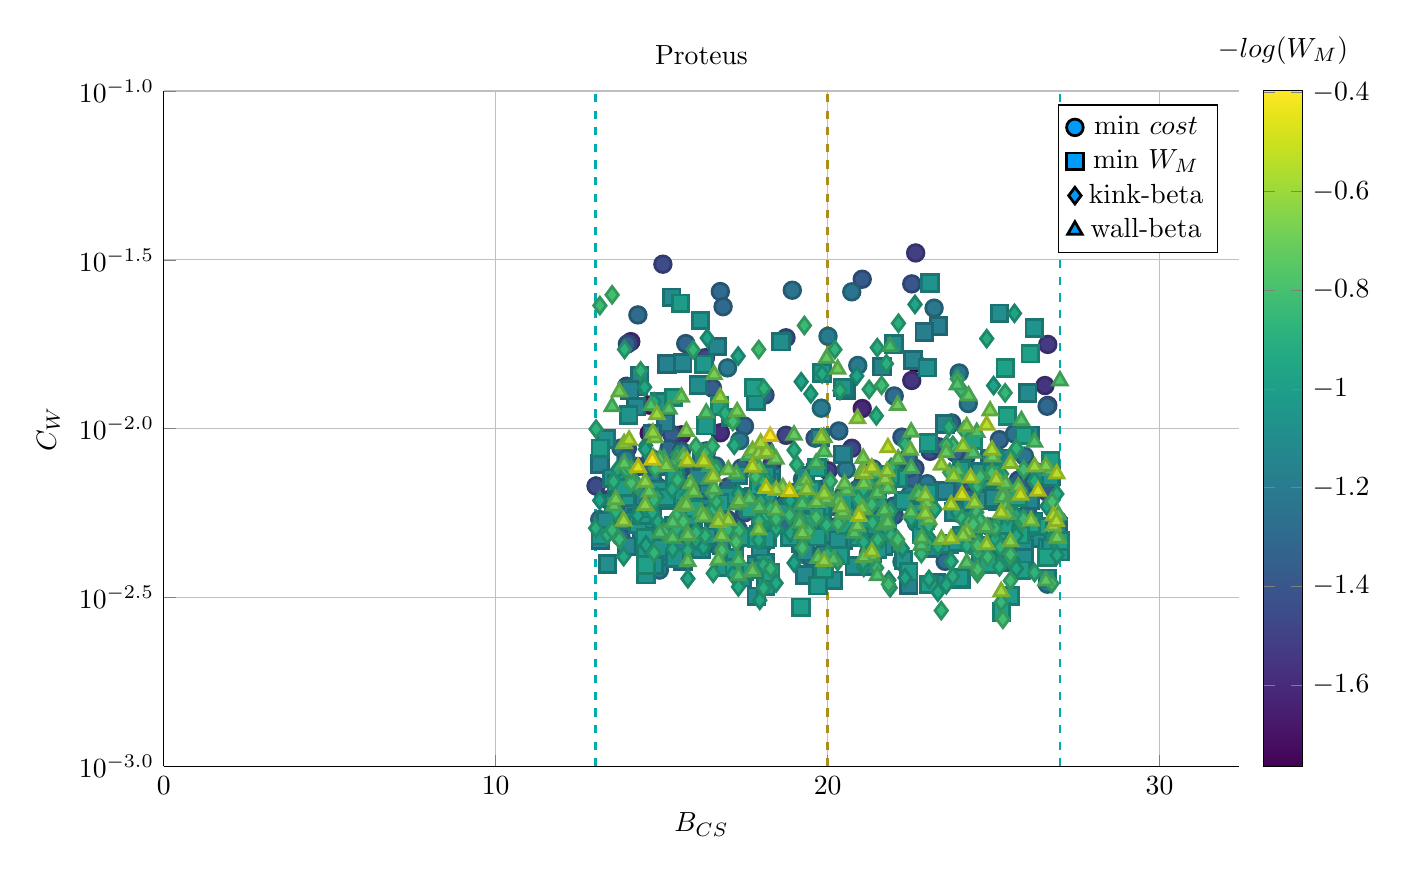
\begin{tikzpicture}[]
\begin{axis}[colorbar = {true}, height = {101.6mm}, ylabel = {${C}_{W}$}, title = {Proteus}, xmin = {0.0}, xmax = {32.398879571197455}, ymax = {0.1}, ymode = {log}, xlabel = {${B}_{CS}$}, {unbounded coords=jump, scaled x ticks = false, xticklabel style={rotate = 0}, xmajorgrids = true, xtick = {0.0,10.0,20.0,30.0}, xticklabels = {0,10,20,30}, xtick align = inside, axis lines* = left, scaled y ticks = false, yticklabel style={rotate = 0}, log basis y=10, ymajorgrids = true, ytick = {0.001,0.0031622776601683794,0.01,0.03162277660168379,0.1}, yticklabels = {$10^{-3.0}$,$10^{-2.5}$,$10^{-2.0}$,$10^{-1.5}$,$10^{-1.0}$}, ytick align = inside, axis lines* = left,     xshift = 0.0mm,
    yshift = 0.0mm,
    axis background/.style={fill={rgb,1:red,1.00000000;green,1.00000000;blue,1.00000000}}
, colormap={plots}{rgb=(0.26700400,0.00487400,0.32941500), rgb=(0.27794100,0.05632400,0.38119100), rgb=(0.28291000,0.10539300,0.42690200), rgb=(0.28229000,0.14591200,0.46151000), rgb=(0.27619400,0.19007400,0.49300100), rgb=(0.26514500,0.23295600,0.51659900), rgb=(0.25042500,0.27429000,0.53310300), rgb=(0.23360300,0.31382800,0.54391400), rgb=(0.21813000,0.34743200,0.55003800), rgb=(0.20123900,0.38367000,0.55429400), rgb=(0.18555600,0.41857000,0.55675300), rgb=(0.17117600,0.45253000,0.55796500), rgb=(0.15772900,0.48593200,0.55801300), rgb=(0.14618000,0.51541300,0.55682300), rgb=(0.13374300,0.54853500,0.55354100), rgb=(0.12346300,0.58168700,0.54744500), rgb=(0.11948300,0.61481700,0.53769200), rgb=(0.12632600,0.64410700,0.52531100), rgb=(0.15014800,0.67663100,0.50658900), rgb=(0.19109000,0.70836600,0.48228400), rgb=(0.24607000,0.73891000,0.45202400), rgb=(0.31192500,0.76782200,0.41558600), rgb=(0.37777900,0.79178100,0.37793900), rgb=(0.45867400,0.81636300,0.32972700), rgb=(0.54552400,0.83803900,0.27562600), rgb=(0.63690200,0.85654200,0.21662000), rgb=(0.73088900,0.87191600,0.15602900), rgb=(0.81457600,0.88339300,0.11034700), rgb=(0.90631100,0.89485500,0.09812500), rgb=(0.99324800,0.90615700,0.14393600)}, colorbar style={title=$-log( W_M )$}}, ymin = {0.001}, width = {152.4mm}]\addplot+[scatter, scatter src=explicit, only marks = {true}, color = {rgb,1:red,0.00000000;green,0.60560316;blue,0.97868012},
draw opacity=1,
line width=0,
solid,mark = *,
mark size = 3.0,
mark options = {
    color = {rgb,1:red,0.00000000;green,0.00000000;blue,0.00000000}, draw opacity = 1.0,
    fill = {rgb,1:red,0.00000000;green,0.60560316;blue,0.97868012}, fill opacity = 1,
    line width = 1,
    rotate = 0,
    solid
}] coordinates {
(22.651942134178245, 0.015650867313707448) [-1.7651507846396934]
(14.624587492471523, 0.009694646552347688) [-1.652530796858066]
(14.624587492471523, 0.011744038729478485) [-1.647000146345283]
(15.59515103457413, 0.009590177278586947) [-1.6184546481250472]
(21.041924335629172, 0.011474300333025303) [-1.6124908438767973]
(16.768060529085655, 0.00972401084478665) [-1.5828949402967583]
(14.070903864396604, 0.018106858351787505) [-1.577618500437912]
(26.63211955782928, 0.011719738653164523) [-1.56873554690934]
(26.54729756362062, 0.013419897432724169) [-1.5599002750009094]
(22.534449427914588, 0.013892471464509717) [-1.5518482038436605]
(26.63211955782928, 0.017767343192357253) [-1.5302287668791192]
(22.651942134178245, 0.033146306422516245) [-1.5115301730224102]
(20.011081752470886, 0.007510212646674021) [-1.5013825191439996]
(20.72766466016537, 0.008751202105526691) [-1.4958902811815062]
(15.146473848919625, 0.00816949735167802) [-1.4892617900728689]
(24.953221543185066, 0.008118078139228204) [-1.4884348201277007]
(18.74607790769805, 0.009559158760396884) [-1.4866425610729714]
(16.318569485171636, 0.01623184139531336) [-1.4835478223239928]
(18.31823242637104, 0.007837831837729894) [-1.4780728724015184]
(15.036815235314387, 0.03069401611625924) [-1.4650031348255397]
(13.023841119875671, 0.006765803188842749) [-1.4601242927308113]
(23.08827436791659, 0.008568870415676909) [-1.453691298071198]
(14.283963091120235, 0.007723927816166263) [-1.4489094778079963]
(13.382063426709323, 0.006162431971740805) [-1.432973868001932]
(18.11370115924847, 0.006329451983138475) [-1.4325147285303634]
(23.34059635854204, 0.008839617844718544) [-1.4268866569895065]
(13.967685136763796, 0.008744700190770928) [-1.4268347679685771]
(18.74607790769805, 0.018590297650719324) [-1.4237681445033143]
(16.531939570236105, 0.007587250291191641) [-1.4234658725845162]
(18.117461030315134, 0.007390656211515189) [-1.4109108269606008]
(18.117461030315134, 0.008694085637837138) [-1.4079262096010774]
(19.068604275965242, 0.00634066157530613) [-1.407330123320285]
(22.534449427914588, 0.026840973164111593) [-1.3996791570309395]
(25.747123007837175, 0.007040053838733538) [-1.3974870797438]
(13.944355842468203, 0.013359280479800206) [-1.3946269662443698]
(22.631885608490197, 0.007634837530984513) [-1.3905305073664083]
(26.612756674676874, 0.006488653571629467) [-1.3895960301339119]
(16.513096841535003, 0.00554611680879456) [-1.381931002288656]
(21.069685019437017, 0.00695131625200887) [-1.3818272949203658]
(21.041924335629172, 0.027704627448181397) [-1.3812563757949996]
(14.736556573901334, 0.00681167564679013) [-1.379699079550137]
(15.578926279356907, 0.006715817539753603) [-1.376650573885692]
(15.578926279356907, 0.00757067906104037) [-1.3758581110553065]
(24.170613812194496, 0.006499559071472007) [-1.375220700855124]
(23.73345635781125, 0.00646934556613389) [-1.3742348635950123]
(18.987744543833536, 0.0063267927368600325) [-1.3713423550361032]
(24.170613812194496, 0.008267480512087599) [-1.370057699317172]
(21.364079170448615, 0.004988896324536347) [-1.3686239973313072]
(22.006250519027304, 0.005540386026064644) [-1.3680076928767484]
(16.643751715736272, 0.005024205798518008) [-1.3672266212882762]
(15.300354897105095, 0.009628839399324697) [-1.3667105305870977]
(25.983749051053568, 0.0050592629231849704) [-1.3651176317240314]
(13.967685136763796, 0.017814080806893125) [-1.3612722200713383]
(15.565992883535738, 0.007840171434328094) [-1.360737823431438]
(16.531939570236105, 0.013182987051350502) [-1.3596008789905631]
(17.009377486662636, 0.006730765435871485) [-1.3568098625263256]
(17.49511712424178, 0.005632641769207446) [-1.3562925407270994]
(23.9635738853514, 0.005613911931897123) [-1.3540300242042478]
(20.336854083719853, 0.005176189759381431) [-1.3527684291391184]
(19.620614991884782, 0.007678792615766904) [-1.3513432280511455]
(25.983749051053568, 0.006888425944911811) [-1.3508742741062625]
(23.84218963638598, 0.006674090356682625) [-1.348444904526092]
(23.73345635781125, 0.010402669872398145) [-1.3482429808137002]
(19.620614991884782, 0.009376571407375644) [-1.3481015746033576]
(18.11370115924847, 0.012583797530216616) [-1.34746159692277]
(22.569231891000115, 0.007115527316776566) [-1.3450418873098828]
(24.492468867569784, 0.006464286011476574) [-1.3449397649071608]
(13.63676824165126, 0.006186516144095541) [-1.344834769873685]
(16.985654434835766, 0.0053864817732829605) [-1.3436955024234147]
(23.84218963638598, 0.00848434463520388) [-1.3426163725681677]
(15.156092946594729, 0.004938310227983135) [-1.3374912582230194]
(19.892081526120066, 0.006636608478826529) [-1.335539302100867]
(21.364079170448615, 0.007606581585076429) [-1.3352915983538123]
(14.277566761363651, 0.006029019944814239) [-1.331337874103357]
(16.34367742556589, 0.008594819258321628) [-1.3310780697195672]
(16.372753180241236, 0.004728216221281147) [-1.3292068036291638]
(18.651304149911, 0.005953363383436291) [-1.32828646244698]
(22.23750424468451, 0.009441137210103956) [-1.3280975618898123]
(14.816548429122673, 0.005079524630506098) [-1.3278697867431468]
(16.278758069854046, 0.005749625528658903) [-1.327757292865828]
(24.236502870832883, 0.006249734903697681) [-1.3253106415861637]
(21.376974447323292, 0.005155209960292018) [-1.3237407060184172]
(17.406035904117076, 0.007650804529712704) [-1.3217246458754282]
(16.676591700948407, 0.004926318213851794) [-1.319376268743699]
(20.218859975126456, 0.004774448071559269) [-1.3182101821558738]
(20.90842789138097, 0.0066268624262571275) [-1.31770129332637]
(15.726344083812931, 0.017867829271260238) [-1.3171626271127284]
(20.509174541398565, 0.006479743346210051) [-1.3144438328362922]
(17.49511712424178, 0.010177994071422254) [-1.314397397461996]
(25.17536025842546, 0.009279261565995508) [-1.3134452963620502]
(16.443823660899717, 0.005896178522672516) [-1.3126768401499638]
(21.376974447323292, 0.007223214696135702) [-1.3123916957087167]
(14.585638446869181, 0.007643344629724278) [-1.3117090270675453]
(14.29222630999366, 0.0062843154751196315) [-1.3112976001573549]
(19.34016378549167, 0.006316305209750007) [-1.3102933400586538]
(26.612756674676874, 0.011655743235665423) [-1.3084666426112759]
(14.677311567391737, 0.008181643780093392) [-1.3081739820914746]
(23.930583881480565, 0.005920113041607297) [-1.3081169022767745]
(18.59998810930447, 0.005266304291939928) [-1.3075986397555424]
(21.639804877968437, 0.0056632699287416785) [-1.3038897119548887]
(14.341073675298674, 0.004515583648974614) [-1.3034916079905217]
(22.44852739031052, 0.00762405310841983) [-1.301506470226052]
(14.283963091120235, 0.021723513711501174) [-1.2978787946122285]
(23.797921766937304, 0.005860560202229156) [-1.297460949292816]
(16.768060529085655, 0.02547444831481485) [-1.2953226778576867]
(16.850723243246257, 0.022974551007964673) [-1.2951062787178942]
(15.221638230176215, 0.008727794605170999) [-1.2946978796261759]
(21.194827607120533, 0.00606442154900928) [-1.293243062455323]
(13.773496878720852, 0.00478216163852665) [-1.2916316854649297]
(16.312384742623273, 0.004505685536187866) [-1.291573412415986]
(19.299286366301942, 0.006201757851874389) [-1.2910367642815292]
(14.715733335251208, 0.007056272547770033) [-1.2894268757747884]
(14.861104082210852, 0.004812007322004063) [-1.2891780169645117]
(21.99387616545991, 0.005900795309436559) [-1.2883016772579983]
(18.07568232599605, 0.004575860387174974) [-1.2877120777365891]
(16.5278219937302, 0.007501625869556503) [-1.2825608117529994]
(23.540570660663604, 0.004048206616482656) [-1.2803416949249293]
(22.006250519027304, 0.012501014524680899) [-1.2790944723531177]
(20.336854083719853, 0.009849033693022476) [-1.2789599032268324]
(21.229554500357366, 0.004266328381972482) [-1.278637308935949]
(14.019194247307421, 0.00602317781329061) [-1.2752962713941192]
(22.427243379042164, 0.008202673797589401) [-1.2724318730764337]
(19.80983944525114, 0.005313590913225172) [-1.26778944603233]
(15.630962235184002, 0.005746237915345085) [-1.2652894696394015]
(16.169659899199626, 0.0063394092295352205) [-1.263844406219344]
(19.370057307761773, 0.004670640784960837) [-1.2622412045786418]
(17.31176227830558, 0.005025369604276285) [-1.2622057750392766]
(17.350614255078973, 0.004715175023029078) [-1.2568407944078956]
(25.92926544649174, 0.005515822538041083) [-1.2564369672634057]
(13.773496878720852, 0.008763742702873716) [-1.255580803936347]
(19.24342166986986, 0.007090160917314494) [-1.2542825781236586]
(25.62853126166569, 0.009658252430988482) [-1.253606675738751]
(16.629549912781222, 0.005078101074449218) [-1.2533258835374417]
(21.331324879071882, 0.004668333949768413) [-1.252740293490489]
(26.02926384975561, 0.005623439530060779) [-1.2512906609771755]
(21.229554500357366, 0.007192663750971734) [-1.2505906665339703]
(26.93045024335227, 0.004753912504004936) [-1.2505667349102745]
(21.770706681119528, 0.00547669175115548) [-1.2505409706978425]
(15.59515103457413, 0.008585550973626429) [-1.2504311283223648]
(26.93045024335227, 0.00536142422310656) [-1.2495193060816674]
(22.748668314502247, 0.005891517799670805) [-1.2472203996667584]
(18.935691126914783, 0.025703839631456088) [-1.246340221801285]
(25.42163009914487, 0.004426672964739238) [-1.246337044553182]
(20.46656298748178, 0.004733745531528537) [-1.2444533586241864]
(19.245483292983383, 0.004373459187272198) [-1.2410504069560844]
(23.9635738853514, 0.014622918962551527) [-1.2404616678069278]
(20.72766466016537, 0.025422666134658947) [-1.2402101811954278]
(26.22602836680247, 0.00699405114862055) [-1.2399625556579728]
(19.15392842040434, 0.005459593535350185) [-1.2395775558220574]
(16.17194115370324, 0.006780135026174841) [-1.238968027160994]
(14.289259863079467, 0.006381273355008305) [-1.2381935518916032]
(19.245483292983383, 0.005454977773134567) [-1.2372164242860222]
(14.084051213081182, 0.006162937475975255) [-1.2359322527835273]
(25.92926544649174, 0.008295248979234676) [-1.2345953253761524]
(13.882021490725897, 0.005661235915534237) [-1.2333782101635051]
(24.89028576683355, 0.005116145429327062) [-1.2329256482335589]
(23.00100122686372, 0.0068738253515159406) [-1.2318041138227]
(16.629549912781222, 0.007759607253139788) [-1.2286780396839752]
(19.836396597287973, 0.004270512991179436) [-1.225800447150557]
(23.207115019583632, 0.022744869820021597) [-1.2237626122718148]
(17.350614255078973, 0.009221148903357415) [-1.2192315569877235]
(24.236502870832883, 0.011868028475244749) [-1.2191811590789894]
(16.34367742556589, 0.008481483201532794) [-1.2185680785343938]
(15.115258956268827, 0.00622802822970762) [-1.2179132583990178]
(14.90981948109104, 0.006703260233628488) [-1.2171472173843672]
(14.749136049291781, 0.00633213628058925) [-1.2167448502658762]
(20.90842789138097, 0.015392818825938645) [-1.2162995250149307]
(17.846164384152665, 0.003872910530196867) [-1.215703789534109]
(20.52604477006502, 0.004720977485089404) [-1.2156312790675603]
(22.124486957585535, 0.00736963569440644) [-1.2145283350978044]
(13.134678555839974, 0.005383150867826381) [-1.214317974252912]
(19.4366251326122, 0.004178935326843822) [-1.2138536176262873]
(26.62064413932083, 0.0034641548226198885) [-1.2119360055173332]
(14.931149108977916, 0.0038140534914709043) [-1.2104347246988538]
(20.557603047451465, 0.007570292211977012) [-1.2084631186053005]
(19.77593528714308, 0.0052385995930077645) [-1.2083264519217767]
(19.161909349795547, 0.005083028024589718) [-1.2073346872626274]
(22.23981527386949, 0.004039129704078142) [-1.2071975929322125]
(16.985654434835766, 0.01513911751066285) [-1.2067840670536927]
(22.486042313795984, 0.006395373245847939) [-1.206736577191552]
(26.236300999552455, 0.007483645463069493) [-1.2065799786199445]
(13.956526564952654, 0.005698374888186277) [-1.203843641047789]
(21.81360757918857, 0.005550896360654382) [-1.203724365314369]
(20.463153166774777, 0.005010777712400389) [-1.2024406864855146]
(14.715733335251208, 0.007157947201399507) [-1.2021169810907544]
(20.011081752470886, 0.01877759730610099) [-1.2015933815507112]
(14.00713301228089, 0.004489267037355289) [-1.2014423796656961]
(13.92658713143997, 0.006374667856956503) [-1.2011965112492808]
(14.486497670639796, 0.00572395742880883) [-1.2005427289121806]
(14.736556573901334, 0.0066192080125215165) [-1.1994215784439877]
(22.133490212694397, 0.007316062816603203) [-1.1975084180232178]
(19.80983944525114, 0.011502671870448664) [-1.1972619972446426]
(22.67137053609239, 0.005266662336518346) [-1.1967371969067386]
(26.735167824179122, 0.004368135902166705) [-1.1965134818457024]
(13.92658713143997, 0.008154332104698897) [-1.196084536648355]
(15.58476565413219, 0.006843978332329513) [-1.1943424204563022]
(25.30217158353333, 0.005029914775543452) [-1.1908054127888088]
};
\addlegendentry{min $cost$}
\addlegendentry{min $W_M$}
\addlegendentry{kink-beta}
\addlegendentry{wall-beta}
\addplot+[scatter, scatter src=explicit, only marks = {true}, color = {rgb,1:red,0.00000000;green,0.60560316;blue,0.97868012},
draw opacity=1,
line width=0,
solid,mark = square*,
mark size = 3.0,
mark options = {
    color = {rgb,1:red,0.00000000;green,0.00000000;blue,0.00000000}, draw opacity = 1.0,
    fill = {rgb,1:red,0.00000000;green,0.60560316;blue,0.97868012}, fill opacity = 1,
    line width = 1,
    rotate = 0,
    solid
}] coordinates {
(15.115258956268827, 0.010422279639263054) [-1.1890033537880158]
(14.715733335251208, 0.009658294464102987) [-1.1883675827161198]
(14.289259863079467, 0.013313745665171912) [-1.1879538738656286]
(19.892081526120066, 0.006487414571263668) [-1.1878029685724296]
(23.34059635854204, 0.020145877705477357) [-1.186260879134981]
(16.751068465480447, 0.005801884747670386) [-1.1859242026174677]
(20.313030948006798, 0.004217349677698315) [-1.183889066210908]
(20.08100946018568, 0.0058827996938258294) [-1.1830291222504283]
(24.89028576683355, 0.008160599297710009) [-1.1826268505607591]
(14.406348579120323, 0.004857174007518612) [-1.182365307189366]
(22.908762374221453, 0.01935279381255584) [-1.1822251925764147]
(20.278362500869783, 0.00447855648592392) [-1.1813612663460882]
(21.35046825241222, 0.00428725320402622) [-1.1785285195809967]
(15.6446694279654, 0.004053651772674214) [-1.1775655951090325]
(26.95198308809553, 0.005121496915389368) [-1.17705398157876]
(14.277566761363651, 0.005890819973806921) [-1.1767452937515073]
(25.12415251137596, 0.006104718148251412) [-1.1766083315756861]
(15.156092946594729, 0.01556268699280997) [-1.173888237216638]
(16.269054087414798, 0.005882961839613334) [-1.1734465174435744]
(20.278362500869783, 0.005961179911412564) [-1.1729466514857931]
(14.227206890976186, 0.006287276174883399) [-1.172839252676928]
(14.119035956708807, 0.005599267038542826) [-1.1727769211527406]
(26.11020939532839, 0.005070632392189801) [-1.1727372361954858]
(22.439521795398957, 0.003434292526080427) [-1.1726542785062386]
(17.248393366297435, 0.0062657093568900535) [-1.1703764252048678]
(16.5796794571122, 0.004942047034638912) [-1.1699166462753263]
(17.970910867302806, 0.004183590560340062) [-1.1681831393061217]
(16.624697426657203, 0.005170881199231806) [-1.1671080842733117]
(16.379855484535224, 0.006777996547666784) [-1.1655606692177785]
(20.463153166774777, 0.008402469668507205) [-1.165303541813206]
(13.151972673873539, 0.004666935296152095) [-1.1643973078802388]
(20.460136716993496, 0.004663766235492665) [-1.1632535008384055]
(19.2031189942159, 0.004566940606242733) [-1.1631989573193973]
(19.83550100861325, 0.0054331000812183365) [-1.1630392685982025]
(23.569327548205543, 0.006544368204474158) [-1.1625753891662707]
(13.671384109436172, 0.006511116933487475) [-1.1617936783337066]
(22.51827341524219, 0.006126048639979384) [-1.159367616011031]
(20.557603047451465, 0.012995381528200805) [-1.1593260324319568]
(18.135261940423753, 0.004013416769217783) [-1.1592024857112633]
(15.652603562708304, 0.004530529794416821) [-1.1590403977294572]
(13.139446789187307, 0.007867971330715704) [-1.1589428109110296]
(16.76328611632, 0.005330271588661515) [-1.158451320077056]
(14.857639167188884, 0.007724720119696045) [-1.157468772898154]
(24.758718787792066, 0.004436262085616985) [-1.1570637161067505]
(16.10076446545596, 0.007249642226094706) [-1.1563966451418943]
(19.77593528714308, 0.009420901412013665) [-1.1561531921827275]
(24.04992975868823, 0.0057898611640113395) [-1.1538328200442942]
(26.735167824179122, 0.007237376261288284) [-1.1525173430901554]
(17.092107947023983, 0.004881019954742076) [-1.1522162283529644]
(17.644214712877762, 0.0059379940430840635) [-1.151968932860403]
(26.108450807284747, 0.0061407721476487214) [-1.1511586507355254]
(21.639804877968437, 0.015255960449664327) [-1.1509834966159156]
(23.06727295287375, 0.004419080970160178) [-1.1503660387736743]
(23.540570660663604, 0.01032617135589161) [-1.1500086948877408]
(25.200810274108626, 0.004014883666259908) [-1.1494080253790357]
(19.32885457468507, 0.005291422749753008) [-1.1493093072503229]
(22.569231891000115, 0.01598351560152435) [-1.1489823622220707]
(21.074369777477393, 0.003915099463846501) [-1.1484511044037433]
(25.27069929453632, 0.005020529922825154) [-1.1483999797493492]
(23.27207804604334, 0.0034947010100993764) [-1.147064765638366]
(14.719150012234948, 0.005859550653426385) [-1.1465028274549764]
(24.247203750488318, 0.005641165149475234) [-1.144883586902141]
(18.31823242637104, 0.007176119328254024) [-1.144368544047569]
(16.20920986207578, 0.00802165691682325) [-1.1435280806157744]
(14.246324004196616, 0.005447269817044685) [-1.1433393449411435]
(25.35315185019304, 0.006668732693209443) [-1.143332108158641]
(19.971681515811508, 0.004886014774808058) [-1.143184585873657]
(16.676591700948407, 0.017515494611674454) [-1.1428249654095861]
(14.341073675298674, 0.014377117697389604) [-1.1427984862828113]
(14.040817864118065, 0.013005276311642224) [-1.142397010267489]
(21.194827607120533, 0.005929095379259443) [-1.1423708774410877]
(15.630962235184002, 0.01565086593371781) [-1.1422424769576425]
(19.32885457468507, 0.007266091038483963) [-1.140012696356206]
(20.5792220239773, 0.005840600330748377) [-1.1399465227440013]
(25.415403683525007, 0.00480284773560221) [-1.1387943392990294]
(19.654837660739332, 0.005752426766742318) [-1.1382802201938975]
(14.227206890976186, 0.011612930840038163) [-1.1380314198362265]
(19.150893512430507, 0.006446360072583165) [-1.137892443914052]
(26.11020939532839, 0.009562541252399106) [-1.1311113631375915]
(20.922532876081345, 0.005743536904522906) [-1.1302954325651586]
(24.59831707555059, 0.0041760314888273755) [-1.1295543261638465]
(14.802199219727623, 0.006161648966500728) [-1.129462828049983]
(19.31280667855182, 0.00369116854025651) [-1.1277963061708562]
(21.467959067562802, 0.006278926396423389) [-1.126807171194116]
(13.95165441994897, 0.004487529275565533) [-1.1267021554022474]
(18.269334848839954, 0.006938744439971839) [-1.1265761162904897]
(19.31280667855182, 0.004304336836767321) [-1.1261385034152473]
(15.968611966724305, 0.005917258047258142) [-1.1260458936236624]
(18.85019132037221, 0.005885263457738176) [-1.1250537668582923]
(14.486497670639796, 0.005616858230043609) [-1.124511019242948]
(17.9238683493206, 0.004843731890681865) [-1.1236988869720232]
(25.85696228036533, 0.005173923137495115) [-1.1235064786985465]
(19.860778911496865, 0.003624821435760545) [-1.1232730371267585]
(18.135261940423753, 0.007429853985811719) [-1.1231293548483412]
(14.36713722146902, 0.005231942783984398) [-1.1209978185544383]
(25.27069929453632, 0.008169617815892689) [-1.1196911148335087]
(24.792905974230315, 0.0061580609115664325) [-1.1194748634113345]
(14.94576539459215, 0.004188882178419093) [-1.119418152841014]
(17.83202655689412, 0.005791769416647159) [-1.1191123923650526]
(21.037434506959272, 0.004931972266091366) [-1.1181736482095217]
(16.33802128070243, 0.005611347227289511) [-1.1176702646643628]
(15.300354897105095, 0.024480989089009208) [-1.1175403888423328]
(16.804752354132532, 0.004518885765871233) [-1.1174827013795072]
(24.9997310960539, 0.0062233325455323925) [-1.1174414411464733]
(13.95165441994897, 0.006299808378708293) [-1.1171134960728113]
(21.91021863095728, 0.004568184715721437) [-1.1171111976535804]
(26.02926384975561, 0.012757776435747556) [-1.1168806186241906]
(18.159403641727735, 0.007305420869085463) [-1.1160945644374545]
(13.321210613736467, 0.005340773800773009) [-1.1139896885893594]
(17.421485223983048, 0.0036233885329560954) [-1.1123768792739945]
(26.198956758292148, 0.005311493039288053) [-1.1112153482766423]
(21.686800668420936, 0.0045000578497955725) [-1.1111283014916062]
(17.850925724336616, 0.003188662256079057) [-1.1108869662710774]
(19.233603569785046, 0.004842654136629077) [-1.1089922492653659]
(25.347291504394295, 0.00452032863173795) [-1.108391782497311]
(14.504420816138161, 0.00535669926333167) [-1.1082929384878708]
(26.32188665435516, 0.004745534590751309) [-1.1074346113685616]
(17.970910867302806, 0.004323464728471098) [-1.1074227437950106]
(17.30594937629188, 0.007293078759243216) [-1.1069130893453907]
(17.850925724336616, 0.003945456212149148) [-1.106325178133445]
(21.792402805381546, 0.004982808461571556) [-1.1060035644106432]
(17.970910867302806, 0.0052409052861536465) [-1.1038776732161713]
(21.069685019437017, 0.0065314531396132094) [-1.10351060592976]
(15.354808162096106, 0.005173060010686301) [-1.1022315889718237]
(17.92907707816459, 0.005951424789746293) [-1.1016702257969113]
(24.59831707555059, 0.007437806150470808) [-1.100448826904311]
(15.948854285961046, 0.005288339533793414) [-1.0998565094908217]
(14.961732146234509, 0.004337170224988449) [-1.0995498480529582]
(25.430993986088392, 0.005750254423520601) [-1.0992970719713648]
(25.92565373787029, 0.004423364554484401) [-1.0987351440216522]
(25.430993986088392, 0.006535275113176343) [-1.0983869460625248]
(21.792402805381546, 0.006822630998366228) [-1.0977261444257258]
(21.99387616545991, 0.017828562633364364) [-1.0969882385788774]
(16.191435661836504, 0.004407786879742766) [-1.096807077081938]
(25.920441712682297, 0.0041501216036249275) [-1.0962033310727437]
(13.367816836249185, 0.003972749736578854) [-1.0948458082881816]
(23.00100122686372, 0.015155543307471772) [-1.093965318294314]
(16.10076446545596, 0.013471957430229371) [-1.093275686079877]
(20.800547804595237, 0.003923510470624812) [-1.0931318196649105]
(18.59998810930447, 0.01811006730780237) [-1.0926393639694263]
(23.797921766937304, 0.005671433069083637) [-1.09199330517098]
(20.172158161026072, 0.0035546432563184145) [-1.0916603258728452]
(25.920441712682297, 0.005082501155756355) [-1.091508438458307]
(21.322964695317083, 0.003922207642532424) [-1.0911853630489914]
(13.508356065492707, 0.007129588907950501) [-1.0896526200520398]
(25.41312647977644, 0.004468466025444819) [-1.088663441639713]
(25.17536025842546, 0.021949864805969728) [-1.0877780715734315]
(13.321210613736467, 0.009322832924906896) [-1.0870739196827126]
(20.321218652713394, 0.004672088916974179) [-1.0855818982110972]
(17.197220657946232, 0.004039319528471343) [-1.0844715994400023]
(13.872957163284784, 0.0053439960085053) [-1.0842780595786392]
(22.748668314502247, 0.005760793758021615) [-1.084266572782003]
(21.108662110316036, 0.00569380985136289) [-1.0839928767281124]
(14.775761073278609, 0.0039349920083461085) [-1.0828594792618813]
(14.806549696522097, 0.0062405207423892875) [-1.082853352734588]
(18.145601806636947, 0.0054577800846403015) [-1.0824719035597]
(24.020772375357197, 0.0035809652689903063) [-1.0824709528228211]
(21.25065104433097, 0.005148297391297789) [-1.0814366033908964]
(15.662032516582798, 0.006582162000449632) [-1.0809878234039578]
(17.764718157329845, 0.006301853688415234) [-1.0808972954130593]
(17.421485223983048, 0.006161790226168522) [-1.0797863646031054]
(26.62064413932083, 0.0036086053477567665) [-1.079163153355685]
(16.368956330173987, 0.004793357206410555) [-1.0780309855478056]
(15.902251231898113, 0.0054298508521766365) [-1.076806285491668]
(19.34016378549167, 0.00604411217248383) [-1.0765985094568509]
(24.032420298396573, 0.004828662165485411) [-1.0760641298404754]
(18.651304149911, 0.005661819547798889) [-1.0757730303287785]
(26.62064413932083, 0.00443044659495794) [-1.0744056068515366]
(15.866386736192135, 0.005467468655559742) [-1.073726482715373]
(24.306579484746003, 0.006046667097602973) [-1.072815333291583]
(17.009377486662636, 0.006315687038558954) [-1.0718638391063322]
(14.931149108977916, 0.011989877345034696) [-1.0710072465261937]
(21.322964695317083, 0.006287200186056995) [-1.0706716976099708]
(26.32188665435516, 0.00739594343637032) [-1.069478881808043]
(17.846164384152665, 0.012080600310741674) [-1.0679830462657767]
(15.30993412600253, 0.006138341400017388) [-1.0670572282884458]
(22.284343035497017, 0.004085658341340117) [-1.0667391835901658]
(17.736283735115194, 0.006004004929014098) [-1.066302608545655]
(14.961732146234509, 0.004440975162005993) [-1.064104157833971]
(23.08827436791659, 0.026972932068461592) [-1.0640878812065675]
(21.508022779864863, 0.004395996587917252) [-1.0635820925869255]
(26.716640036139204, 0.004423420241739423) [-1.062988318250961]
(19.11527100708343, 0.00480727122317776) [-1.0628036997189863]
(18.131669417857122, 0.0034131330547271113) [-1.062700357913494]
(14.529712726466656, 0.0036974585830479817) [-1.0626514373993834]
(18.173944283111027, 0.004776499853086686) [-1.0610739421064752]
(15.401502456170876, 0.004144297606935685) [-1.0588352037418618]
(16.169659899199626, 0.0209014980088616) [-1.0585986545827941]
(14.00713301228089, 0.010988948677442597) [-1.057135771526312]
(20.46656298748178, 0.013241941603829825) [-1.056315661795303]
(26.22602836680247, 0.019862106250452566) [-1.0562734967702754]
(22.819346636869057, 0.004858658731965693) [-1.0561257856094448]
(19.11527100708343, 0.006223828461257365) [-1.0559814704124602]
(18.131669417857122, 0.004706089102701761) [-1.0555859489072712]
(18.079332919029085, 0.003994614402213268) [-1.0549803415205259]
(20.87914774430368, 0.006463993798881436) [-1.0545713902023608]
(16.908681604757444, 0.0038990516235787613) [-1.054205756099488]
(26.711777515939247, 0.007195479612398366) [-1.0536290024409787]
(13.929572546627387, 0.006286763322784177) [-1.0533216125601341]
(13.151972673873539, 0.004822724612666477) [-1.0529307720930816]
(22.819346636869057, 0.005656264568736301) [-1.0525850668019536]
(15.477350070944595, 0.006295530789348686) [-1.052552508886994]
(24.032420298396573, 0.007550888758433211) [-1.0509835312174363]
(15.45268981247694, 0.004904482654727138) [-1.0508250621973283]
(14.961732146234509, 0.006571304536184572) [-1.050680345054969]
(23.655268515644366, 0.004560195418506711) [-1.0506245233592775]
(17.092107947023983, 0.01080264515897382) [-1.0505217359121972]
(13.55338844221082, 0.00597835329976134) [-1.049317623712287]
(17.625908695494353, 0.00605275476812188) [-1.0490747591885061]
(24.537224497440306, 0.004511808104116367) [-1.0489907539423449]
(24.391233921325668, 0.0049153150140211965) [-1.0478434867034416]
(23.909126603799116, 0.004616652674773231) [-1.0473758850488442]
(18.173944283111027, 0.006447737760929581) [-1.046767629611379]
(22.284343035497017, 0.006114416229637186) [-1.0460742739305466]
(19.83550100861325, 0.01461141466329314) [-1.0428746875530057]
(19.710045895289856, 0.0034297894059699906) [-1.0409932776852704]
(26.99666218082735, 0.004324846597058025) [-1.040720375777512]
(13.63676824165126, 0.0068957525832947) [-1.0400494553390642]
(18.87182730714039, 0.0047742837106654985) [-1.03963800286999]
(24.953221543185066, 0.0070972253563865) [-1.0394862991533038]
(20.509174541398565, 0.006107051538135721) [-1.0391370640013136]
(16.278758069854046, 0.015503036624972183) [-1.038354289214968]
(23.035515049672192, 0.006445735380428859) [-1.0380750082543837]
(14.279438101093232, 0.005205902574339689) [-1.0370263081612092]
(21.737554950575895, 0.005283195240312258) [-1.0365321066837632]
(19.806577545472447, 0.005892181423629392) [-1.0364145571368009]
(16.33802128070243, 0.010214094301379546) [-1.0358730287795153]
(17.48698733172037, 0.003781581128188247) [-1.0352797650690977]
(21.495458720132525, 0.0061316127141858145) [-1.0352425491421158]
(14.518866161482416, 0.004345014451914255) [-1.0335536367675167]
(17.197220657946232, 0.00415632052734694) [-1.0319535365225938]
(15.134079464405815, 0.006253917955260214) [-1.031638330454266]
(23.993469701679754, 0.003613822408322808) [-1.0316283345953763]
(17.48698733172037, 0.00478160347928963) [-1.0312630056422283]
(24.747450186073678, 0.004326998549376461) [-1.030801418278412]
(16.751068465480447, 0.006039359373565179) [-1.0301227610636083]
(14.406348579120323, 0.005550817437725965) [-1.029015666765989]
(19.493426492317983, 0.006583295742064639) [-1.0288573869793878]
(20.37163275163815, 0.004204292638824563) [-1.0245024368116802]
(15.401502456170876, 0.007145400138218064) [-1.0231385619546913]
(19.68119459959854, 0.004789677204757558) [-1.021449027000752]
(17.924682632407837, 0.00675373673736514) [-1.0213127693885564]
(25.50482023490044, 0.003193542226257652) [-1.0209276741398987]
(22.124486957585535, 0.007121099635585821) [-1.0202684704954939]
(22.439521795398957, 0.0037708668397859442) [-1.0187837906200732]
(15.743591734002468, 0.005805595496214904) [-1.0179738483919518]
(23.035515049672192, 0.009070154520460257) [-1.0169425110693646]
(15.5630871969197, 0.00501503870041615) [-1.0162045101447212]
(13.869405436882781, 0.00670010251636303) [-1.0149810946438107]
(13.151972673873539, 0.008752580219573484) [-1.014353466976016]
(15.565992883535738, 0.023528952793841592) [-1.0140528730661398]
(19.665351838058136, 0.005527004085356763) [-1.0133093427968076]
(20.943775733817652, 0.004778958682375364) [-1.0128360857902137]
(18.033648098721542, 0.003842216867194081) [-1.0126834015105255]
(21.878860060352352, 0.007300503854095673) [-1.0124869131348806]
(25.83788180341901, 0.0038089628255598917) [-1.0084966915198963]
(26.716640036139204, 0.008048423371546378) [-1.005776006726422]
(26.339525393761082, 0.005136336479510988) [-1.0027757315503723]
(19.193829077288807, 0.0029594317443149176) [-1.002422823826331]
(23.0540274641531, 0.003459304695059543) [-1.0023352556688647]
(25.143925437510074, 0.004988217345842403) [-0.9994656987080655]
(26.999066309331212, 0.004649343635980374) [-0.9991953302395459]
(24.969602727169466, 0.007411548557741582) [-0.9991876183275935]
(17.18725041495652, 0.0038831217844692545) [-0.9971256954762724]
(25.239953702493796, 0.0028654321699102935) [-0.9968293366364798]
(24.38577334322156, 0.004992975570566671) [-0.9965130838642419]
(19.895557019888, 0.003830578946172306) [-0.9960911988132904]
(17.764718157329845, 0.013215773066776348) [-0.9953080727443692]
(22.937595078654155, 0.005338097758519931) [-0.994764309342816]
(14.62322740320338, 0.005798704578553127) [-0.9941918143808477]
(19.68119459959854, 0.007661762309327555) [-0.9939974184414383]
(15.354808162096106, 0.012372283627325148) [-0.9936895922796631]
(14.509582689075785, 0.0047417231470052315) [-0.9920762514365737]
(25.357682218729416, 0.005175409039233765) [-0.9891335090238219]
(17.644214712877762, 0.005799134035216279) [-0.988320863141931]
(24.822975077806525, 0.003975692742134705) [-0.9873980470532571]
(15.968611966724305, 0.005803966541873779) [-0.9872638091155089]
(19.372259092318934, 0.005281651647264406) [-0.9871243344745786]
(25.92565373787029, 0.00954881671016918) [-0.9862026242600886]
(24.391233921325668, 0.009231911938640338) [-0.9851939256634008]
(26.125739860092395, 0.005233428706224578) [-0.9845137991026185]
(25.35315185019304, 0.015110407509335635) [-0.9844063088607684]
(25.747123007837175, 0.006274740712107015) [-0.9843851675543582]
(26.108450807284747, 0.01666579340898781) [-0.9832677624207663]
(17.860630065422363, 0.004743145828135927) [-0.9823156156623659]
(18.28268228926236, 0.003744148435661381) [-0.9817957805945331]
(25.812435546384016, 0.0048552692105239565) [-0.9817262777133879]
(16.751068465480447, 0.01167873981501713) [-0.980944500204026]
(26.605009277171177, 0.004161496814710868) [-0.9808435285359967]
(25.41312647977644, 0.010903168023481107) [-0.9803069086017846]
(20.536092995679923, 0.005187973951951495) [-0.979926239566149]
(14.529712726466656, 0.0039527765780552285) [-0.9799255860420428]
};
\addlegendentry{min $cost$}
\addlegendentry{min $W_M$}
\addlegendentry{kink-beta}
\addlegendentry{wall-beta}
\addplot+[scatter, scatter src=explicit, only marks = {true}, color = {rgb,1:red,0.00000000;green,0.60560316;blue,0.97868012},
draw opacity=1,
line width=0,
solid,mark = diamond*,
mark size = 3.0,
mark options = {
    color = {rgb,1:red,0.00000000;green,0.00000000;blue,0.00000000}, draw opacity = 1.0,
    fill = {rgb,1:red,0.00000000;green,0.60560316;blue,0.97868012}, fill opacity = 1,
    line width = 1,
    rotate = 0,
    solid
}] coordinates {
(21.711893029131566, 0.0049343734079309275) [-0.9797193514246809]
(20.87914774430368, 0.014326928101993836) [-0.9793649258547107]
(22.249101100040285, 0.004418560150536774) [-0.9793554194238832]
(23.993469701679754, 0.007133046942930264) [-0.9793399260652301]
(14.529712726466656, 0.004527202123528333) [-0.9786718824413932]
(19.2031189942159, 0.013777079521683793) [-0.9784247640598123]
(25.079354543031585, 0.005278344797288595) [-0.9784156054323705]
(18.989026003231032, 0.004002965553163199) [-0.9772101816150688]
(24.9997310960539, 0.013418113026562503) [-0.9771245449599791]
(25.62847037709553, 0.004027289040267911) [-0.9768013676267739]
(16.372753180241236, 0.018551171796247393) [-0.9763993914483391]
(13.134678555839974, 0.006130885121857039) [-0.9762949474128021]
(16.427208297726143, 0.005562603331167774) [-0.9759999361809304]
(25.143925437510074, 0.008328856003390762) [-0.9748577786630778]
(19.99680496969866, 0.004109700372311695) [-0.9738966318394574]
(13.56697824167195, 0.004913914166672265) [-0.9734793512186626]
(16.03107337465876, 0.004665122126804512) [-0.9731032751395803]
(18.033648098721542, 0.006640697404806304) [-0.9726016535105552]
(24.427094392002633, 0.004736078134325021) [-0.9724572780741577]
(23.908352016960492, 0.005647304198937851) [-0.9722087723669882]
(24.79132961055872, 0.004389286248628818) [-0.9718244022964762]
(22.332295899617375, 0.0036192646662402627) [-0.970582002945255]
(13.671384109436172, 0.007574170243236733) [-0.9693863160362324]
(17.30594937629188, 0.016406094197261946) [-0.968978562403945]
(18.87182730714039, 0.004910644527520683) [-0.9682987091511867]
(21.62636840883897, 0.004713875842941002) [-0.9661896439247507]
(19.193829077288807, 0.005899389733384474) [-0.96458538139874]
(21.793166599979934, 0.0056286885015633895) [-0.9644132418595727]
(16.260430864278227, 0.004458328702018249) [-0.9642494738631832]
(26.605009277171177, 0.005896947846453336) [-0.9638749980488863]
(14.518866161482416, 0.008919099387898428) [-0.9633607889353855]
(17.144948028029052, 0.003704995647544644) [-0.9628913890413714]
(18.87182730714039, 0.00612171997200749) [-0.9627420883815555]
(21.843108678301228, 0.003560196433315863) [-0.9623524414535783]
(25.62853126166569, 0.02195538724653361) [-0.9620751879990892]
(17.955918213319755, 0.0031037314795763953) [-0.9616273380898692]
(23.06727295287375, 0.004737846584498155) [-0.9614728013262]
(22.9924640163578, 0.0056288454988440186) [-0.9611621976310423]
(17.31176227830558, 0.006420794710655912) [-0.9607076853432408]
(25.68282437564652, 0.004827398822111102) [-0.9600064809118957]
(22.631885608490197, 0.02333271298987377) [-0.9582788764682687]
(25.68282437564652, 0.005548252171458194) [-0.9582126253448857]
(23.06727295287375, 0.005664193052715976) [-0.9580357625022031]
(14.279438101093232, 0.005536719771654066) [-0.957784719926681]
(25.68559192901304, 0.003853864382102105) [-0.9569481934101607]
(16.556270886342375, 0.005755412847229535) [-0.9553125817248839]
(14.509582689075785, 0.008689466677368552) [-0.9542931196842905]
(16.58107133568487, 0.0059335279307082415) [-0.9535689234008579]
(22.517026888269854, 0.00540418577910244) [-0.9533577705177119]
(20.77275422833572, 0.004951751523060612) [-0.9524896594035642]
(15.790739414166003, 0.0035965091424978767) [-0.9519498604980341]
(16.804752354132532, 0.005225320910765454) [-0.9518141933322811]
(21.467959067562802, 0.0064487141747247515) [-0.9516817791582881]
(26.80433260075194, 0.004824944888873151) [-0.9503280372896984]
(24.08056889459325, 0.00494548994415281) [-0.9501901690400224]
(14.861104082210852, 0.005348280279251544) [-0.9501200807106565]
(23.575238252030694, 0.003451161099821506) [-0.9494094470373718]
(19.493426492317983, 0.012679296138241048) [-0.9485432404545778]
(14.861104082210852, 0.006306624155522614) [-0.9476409244484506]
(14.486497670639796, 0.013277570668597095) [-0.945668217439486]
(14.775761073278609, 0.012011087422302516) [-0.9455646191283261]
(26.913506127016916, 0.0042225651663969944) [-0.9452539976263535]
(21.817575837477094, 0.007400046119087899) [-0.9445379968061569]
(21.088494147417737, 0.0038853521635503845) [-0.9442842771351952]
(23.0540274641531, 0.003581425300578328) [-0.9439633256599537]
(19.836396597287973, 0.014533706969027229) [-0.9435190061725043]
(21.495170330924516, 0.005251128867230356) [-0.9431579759120018]
(23.32241055960176, 0.0032803092315458883) [-0.9428483368499935]
(16.76328611632, 0.005138967929828396) [-0.9422331530579936]
(18.447686620108747, 0.0034905159514662587) [-0.9396609276523904]
(21.074369777477393, 0.004029446318551389) [-0.939623008122614]
(23.0540274641531, 0.00455015926208741) [-0.9389137302612279]
(15.33021544852462, 0.00439803335731196) [-0.938282475354221]
(18.159403641727735, 0.007076676002554203) [-0.9381610470878076]
(13.855662151001413, 0.004180164094848145) [-0.9375089447207223]
(25.047879452913545, 0.0047224227678250175) [-0.9369328543779993]
(17.98391484948191, 0.0060949751266714085) [-0.9362670591806482]
(14.719150012234948, 0.005648330019282998) [-0.9352069487820426]
(24.387769811025546, 0.005000154489324483) [-0.9348472459577944]
(17.955918213319755, 0.005297957377087851) [-0.9342522553820941]
(21.495170330924516, 0.006759629185969791) [-0.9338432220939059]
(15.30993412600253, 0.006608248212098614) [-0.9331696663167082]
(23.32241055960176, 0.004476157560195598) [-0.9323821674335669]
(22.834131439170747, 0.004553679627799357) [-0.9312147370194936]
(24.537224497440306, 0.004658130964295737) [-0.930280167995953]
(18.447686620108747, 0.005060711761627857) [-0.9280045677807334]
(24.792905974230315, 0.018476285473848813) [-0.9280031254185547]
(17.312868144499753, 0.0034004941489706427) [-0.9276368843131759]
(24.59404027903679, 0.005166624841841688) [-0.9268239261037757]
(15.785946454503529, 0.004359745755123362) [-0.926124917347277]
(23.23495821442244, 0.005775582114052551) [-0.9257073204007308]
(17.18725041495652, 0.008935057639573897) [-0.924623493423007]
(19.158825560243013, 0.005284834073095107) [-0.9243237059537647]
(24.387769811025546, 0.006960808141066332) [-0.9233834598837832]
(24.764249505652145, 0.004477816754705252) [-0.9228152651263011]
(15.610110935591706, 0.005256266572834143) [-0.9225398322566478]
(21.086014975073198, 0.004614605578452094) [-0.9221817845745035]
(17.9238683493206, 0.004684328138894626) [-0.9215264386089611]
(13.011374727983977, 0.005073667236310502) [-0.9182360577808578]
(26.236300999552455, 0.00699448652183368) [-0.9171606639000199]
(25.496539583465434, 0.004096269252840535) [-0.9167994991962954]
(24.105981493227365, 0.004877105036737716) [-0.9148199077007076]
(18.145601806636947, 0.005333658362398189) [-0.9143950266851926]
(15.772215710533262, 0.0063326000908344015) [-0.9137204603649657]
(23.77209082045688, 0.003656199076187517) [-0.9133127453951064]
(26.905013263566943, 0.006406059775809559) [-0.9121627392578615]
(21.843108678301228, 0.006847766811629225) [-0.9120709030515949]
(21.074369777477393, 0.006587871594639965) [-0.9120475096142877]
(24.537224497440306, 0.006957117514637042) [-0.9120417957644669]
(21.88346447009828, 0.003379934383470047) [-0.9119544487627024]
(21.467959067562802, 0.010913194864582846) [-0.911708891151293]
(20.30332931675502, 0.004041226194685478) [-0.9111798161472054]
(25.239953702493796, 0.0073486956507704685) [-0.9107411837742436]
(26.79882485524314, 0.004735506056694406) [-0.9100560207797687]
(23.655268515644366, 0.010112207946458425) [-0.9096645202732524]
(18.989026003231032, 0.008635225183072814) [-0.9087883894803973]
(21.686800668420936, 0.005403661462545021) [-0.9082790009204854]
(23.71920555338414, 0.004047054134608013) [-0.9081431792626627]
(25.17696423356227, 0.003902974011235298) [-0.9067699437470415]
(21.495458720132525, 0.017382642208156447) [-0.9060971962820227]
(24.194837362132866, 0.004507017121233361) [-0.9060048430542386]
(18.442422810906905, 0.0054677225459759575) [-0.9051444524245076]
(19.99680496969866, 0.004250447610661418) [-0.9046954309394458]
(25.42163009914487, 0.005523706134151735) [-0.9046460109599029]
(15.469368499099941, 0.005058679669540388) [-0.9046042329773717]
(19.15808110804699, 0.004880341290688154) [-0.9039977279126346]
(13.367816836249185, 0.004848014991264962) [-0.9034337968845987]
(18.072238642477593, 0.0033710581928259836) [-0.9031566859943262]
(22.133490212694397, 0.02051608060889296) [-0.9023267465363606]
(18.072238642477593, 0.00394866132787808) [-0.9008355008980751]
(16.908681604757444, 0.011116102682336754) [-0.9007285357561787]
(16.552565712961382, 0.0037301270643077876) [-0.8972742280672815]
(13.55338844221082, 0.006975150409970039) [-0.897175036870542]
(24.511261732188537, 0.004282665596744035) [-0.8971186814881362]
(20.37163275163815, 0.012972814791692319) [-0.8969796612342156]
(23.05056195453426, 0.0051618357133361315) [-0.89672282177903]
(21.770706681119528, 0.015575744813995764) [-0.8963952627105445]
(18.269334848839954, 0.006658522954563811) [-0.8958485488547734]
(18.07568232599605, 0.005404120857058153) [-0.8943684288096996]
(22.332295899617375, 0.009007603010797853) [-0.8914082601651864]
(18.07568232599605, 0.006944169371814818) [-0.8896483571913044]
(19.99680496969866, 0.006491642132230442) [-0.8869865112217631]
(13.023841119875671, 0.009974107942199384) [-0.8866075677924622]
(18.079332919029085, 0.013162396177814029) [-0.8851823316418669]
(21.91021863095728, 0.004826124490303322) [-0.8846740900795415]
(13.616480154545364, 0.005684202227253982) [-0.8840192815000373]
(16.312384742623273, 0.0048201007942522064) [-0.8839767416908659]
(19.068604275965242, 0.007830361841197038) [-0.8835453569153728]
(19.968999576205356, 0.005186138093663713) [-0.8832514898254401]
(17.93627510472957, 0.0053254692875210185) [-0.8832295476215102]
(25.62847037709553, 0.008573190683116311) [-0.883069564455261]
(25.200810274108626, 0.004462559243137306) [-0.8830632191913902]
(21.88346447009828, 0.005696949886972815) [-0.8825797897872378]
(13.882021490725897, 0.01716789737474233) [-0.8801231316414504]
(21.35046825241222, 0.005269633409728344) [-0.8791867595932125]
(20.922532876081345, 0.006190708259408953) [-0.877951083604425]
(21.25065104433097, 0.013073202281995273) [-0.8774262288873376]
(15.902251231898113, 0.006886241915548495) [-0.8751523935645794]
(26.232326861807465, 0.003750268079957199) [-0.8748921304141444]
(14.36713722146902, 0.014828542032509849) [-0.874690516784764]
(14.771138015954458, 0.004289107281658671) [-0.8742887892359985]
(16.58107133568487, 0.005786133363621624) [-0.8739921539442262]
(25.68559192901304, 0.008747322528766296) [-0.8716524887679293]
(20.218859975126456, 0.01715728174165555) [-0.8712831508374237]
(15.469368499099941, 0.008344053133431154) [-0.8707782727491976]
(24.511261732188537, 0.006756312980238707) [-0.8688158783682262]
(17.009893524049446, 0.005033506475358252) [-0.8686482360373176]
(16.643751715736272, 0.0060832943243140855) [-0.8685858440662988]
(16.03107337465876, 0.004920623586218273) [-0.8672784286683882]
(19.370057307761773, 0.004866417685086465) [-0.866786932045215]
(25.17696423356227, 0.007171410952306857) [-0.8662743883953999]
(21.508022779864863, 0.004690311648627596) [-0.8651646039969739]
(16.643751715736272, 0.007587597698564831) [-0.8649542416484729]
(16.20920986207578, 0.008493030870048135) [-0.8638854242016366]
(21.91021863095728, 0.007681026757569149) [-0.8637850725340939]
(18.28268228926236, 0.00385351424497451) [-0.8621520373035888]
(24.04992975868823, 0.005420954062013184) [-0.8611949292176813]
(25.347291504394295, 0.012767830297498842) [-0.8597568594294163]
(23.423616029838065, 0.0028935280651521448) [-0.859303050958753]
(15.477350070944595, 0.007054888627501927) [-0.85891018749718]
(13.508455039987684, 0.005004853345841743) [-0.8586165859116928]
(24.105981493227365, 0.009908479871966714) [-0.8586114389950454]
(14.771138015954458, 0.006151478093055551) [-0.8583221454358831]
(19.370057307761773, 0.006469455145345583) [-0.8577258338037467]
(24.247203750488318, 0.0052827318377912606) [-0.856994532353176]
(25.228628745964095, 0.0030638188926231558) [-0.8566075426873476]
(16.379855484535224, 0.008039114601071939) [-0.8562684441084778]
(15.948854285961046, 0.01712944125320649) [-0.8558052872802134]
(22.824087425680514, 0.004267584417782998) [-0.8545697779334551]
(16.312384742623273, 0.008482681890822595) [-0.8538958276429577]
(21.47813011726619, 0.003872739374790015) [-0.8535463695644936]
(16.5278219937302, 0.008873113176598642) [-0.85173359228685]
(25.047879452913545, 0.0050732777646726) [-0.8517054901788327]
(13.726047247124878, 0.004701607268823488) [-0.8493774101081241]
(19.158825560243013, 0.005419475274884782) [-0.8484701682854062]
(22.937595078654155, 0.00613724465859049) [-0.8467333432677736]
(13.929572546627387, 0.007557168723331712) [-0.8464349448005866]
(25.85696228036533, 0.005291739209830012) [-0.8453378253842451]
(17.331198319361267, 0.004983376401809511) [-0.8450087852753472]
(24.51457558642517, 0.003726820437409142) [-0.8448171197590391]
(18.28268228926236, 0.005789125924199343) [-0.8432574743352121]
(18.85019132037221, 0.005549754850410065) [-0.8430436771013377]
(14.277566761363651, 0.006783858344365182) [-0.8427718589011481]
(25.903908026071807, 0.005406145285483184) [-0.8415948084087838]
(18.448679664153556, 0.005406021522066206) [-0.8413272380615733]
(21.331324879071882, 0.005966658469646099) [-0.840505435392519]
(14.246324004196616, 0.006853609897202617) [-0.8403240064715908]
(20.409971582846815, 0.005315540207414598) [-0.8379028159133117]
(16.03107337465876, 0.008857688291635324) [-0.8377789816141492]
(14.90981948109104, 0.007938563015546142) [-0.8372578650925528]
(24.822975077806525, 0.004170239875860694) [-0.8369045170441011]
(24.492468867569784, 0.0056579135553807185) [-0.8359444642160421]
(23.77209082045688, 0.008931755340602409) [-0.8352235482527809]
(20.08100946018568, 0.006981447071324104) [-0.8348048184219272]
(26.75919220891685, 0.0034808725102794254) [-0.8343383061127448]
(13.139446789187307, 0.023150613766082406) [-0.833965424798725]
(24.020772375357197, 0.0130684108929944) [-0.8330108332095327]
(19.299286366301942, 0.02020816396851675) [-0.8328999767795251]
(24.822975077806525, 0.005117909063290362) [-0.8325894160918027]
(23.575238252030694, 0.008942904219591468) [-0.8305235366709506]
(24.59404027903679, 0.005329721235361873) [-0.8279917628427604]
(21.62636840883897, 0.013442707154089855) [-0.8257253077335049]
(19.4366251326122, 0.004961296668951894) [-0.8244439870918499]
(25.50482023490044, 0.003549416514808207) [-0.8243214968512095]
(15.070376902383966, 0.004936273572913412) [-0.8242933470610456]
(16.513096841535003, 0.006450216216685992) [-0.823012819256833]
(14.806549696522097, 0.0076278023903487095) [-0.8223450782723788]
(25.50482023490044, 0.004240662831829435) [-0.8222030505336514]
(22.113655252880513, 0.004583574206680189) [-0.8220930638276832]
(25.903908026071807, 0.007568987706711713) [-0.8220631016600264]
(15.45268981247694, 0.005518205902757275) [-0.8219864216086542]
(20.313030948006798, 0.005230785495605878) [-0.8219312934239001]
(23.908352016960492, 0.014042771210954628) [-0.8200917106540455]
(20.536092995679923, 0.0057025663921860025) [-0.8199389869999576]
(21.83179616436196, 0.003461216371181937) [-0.8184296236132867]
(24.59404027903679, 0.007217320297822837) [-0.8176734758564849]
(19.239362922333935, 0.004437347255537501) [-0.8154036160329199]
(17.924682632407837, 0.01716089273801921) [-0.8153527954342572]
(17.83202655689412, 0.007223735861818005) [-0.8144082854197419]
(17.144948028029052, 0.010504588562265854) [-0.8128175200037216]
(19.654837660739332, 0.005469791669344847) [-0.8124816458921246]
(15.45268981247694, 0.00800956789757918) [-0.811311819724745]
(13.508356065492707, 0.024915969416016464) [-0.8111026189728189]
(22.110321392556187, 0.004696885840713195) [-0.8093556032871382]
(23.676571204968464, 0.007424815290696485) [-0.8081403395005344]
(25.279679700751608, 0.002726446890806165) [-0.8078565007546591]
(19.886196105853493, 0.004060122004748655) [-0.8076401136101801]
(24.38577334322156, 0.00521133009673052) [-0.8058609898285525]
(15.652603562708304, 0.005311081041698119) [-0.8047538384635771]
(15.785946454503529, 0.004818293923541147) [-0.8045321061264834]
(26.75919220891685, 0.006080023629405084) [-0.804095594882759]
(14.084051213081182, 0.006910473351855834) [-0.8037221310081099]
(15.58476565413219, 0.008100775387463259) [-0.8035470296524466]
(14.084051213081182, 0.007575262106447099) [-0.8029316931085251]
(24.953221543185066, 0.007394228868903094) [-0.8027212756805284]
(24.51457558642517, 0.0038334779249383955) [-0.8021950738645045]
(17.24469713700245, 0.004623754785007905) [-0.8001182754285723]
(24.51457558642517, 0.004516682923706159) [-0.8000707725554996]
(16.807954356556944, 0.0043544029690039685) [-0.7981120109543962]
};
\addlegendentry{min $cost$}
\addlegendentry{min $W_M$}
\addlegendentry{kink-beta}
\addlegendentry{wall-beta}
\addplot+[scatter, scatter src=explicit, only marks = {true}, color = {rgb,1:red,0.00000000;green,0.60560316;blue,0.97868012},
draw opacity=1,
line width=0,
solid,mark = triangle*,
mark size = 3.0,
mark options = {
    color = {rgb,1:red,0.00000000;green,0.00000000;blue,0.00000000}, draw opacity = 1.0,
    fill = {rgb,1:red,0.00000000;green,0.60560316;blue,0.97868012}, fill opacity = 1,
    line width = 1,
    rotate = 0,
    solid
}] coordinates {
(21.878860060352352, 0.017490077363632575) [-0.796569715037787]
(21.194827607120533, 0.006971446105088665) [-0.79441004262747]
(14.94576539459215, 0.004911921812799429) [-0.7933559474809188]
(17.24469713700245, 0.005954017273857897) [-0.793170820712885]
(15.652603562708304, 0.007955591590128024) [-0.7930383455051904]
(19.654837660739332, 0.007901931985354861) [-0.7901570548309161]
(15.070376902383966, 0.008137353095022991) [-0.7899846868276869]
(22.824087425680514, 0.00451444584006381) [-0.7877812779595144]
(24.492468867569784, 0.009753587016237195) [-0.7866817518906072]
(21.50197112243447, 0.003671094509078405) [-0.7862115386558454]
(19.233603569785046, 0.005984919625817065) [-0.7857827687264937]
(16.443823660899717, 0.007731178757598179) [-0.7852361561866921]
(16.368956330173987, 0.005487637707476247) [-0.7839377375933054]
(17.312868144499753, 0.0036719603734188056) [-0.7819628551532836]
(19.15808110804699, 0.0052571395699657075) [-0.7811216845856691]
(26.999066309331212, 0.013864387522447816) [-0.7809918721633216]
(17.312868144499753, 0.004076457809715312) [-0.7809175837352759]
(23.909126603799116, 0.01348942620030939) [-0.7808076935800926]
(24.38577334322156, 0.008463888793993459) [-0.7806814861016669]
(23.930583881480565, 0.007481884358420134) [-0.7801570592845017]
(26.232326861807465, 0.009121533238626805) [-0.779570124080519]
(17.625908695494353, 0.008320597960456288) [-0.7795292440734509]
(18.31823242637104, 0.008435833537480966) [-0.7778143736900492]
(14.94576539459215, 0.008142288298726664) [-0.7773545006224067]
(21.83179616436196, 0.006689457230456803) [-0.7764899368885182]
(20.800547804595237, 0.0049083517753881175) [-0.7756195405244002]
(26.711777515939247, 0.007521529262855716) [-0.775153683924341]
(15.33021544852462, 0.004740003739998331) [-0.7750610829327748]
(19.15392842040434, 0.006724172004779728) [-0.7747436949495959]
(14.677311567391737, 0.011698217503304088) [-0.7742992479600759]
(22.67137053609239, 0.006405289888306118) [-0.7742009181502876]
(15.33021544852462, 0.005273402730059259) [-0.7740650517521674]
(21.47813011726619, 0.007399875727122566) [-0.7739873317108487]
(16.34367742556589, 0.01112021819603376) [-0.7725628696347435]
(20.172158161026072, 0.004092971739154845) [-0.7712605585908249]
(13.508455039987684, 0.011622544197713853) [-0.7710828598045486]
(17.93627510472957, 0.005847108178504653) [-0.7673997285740343]
(24.190608387466142, 0.004002837382643835) [-0.7673383740621305]
(22.748668314502247, 0.006406320488396418) [-0.7672456113797256]
(16.191435661836504, 0.005660698191622548) [-0.764435393058592]
(15.221638230176215, 0.011426609842125667) [-0.7638357297225782]
(22.51827341524219, 0.007631339242334709) [-0.7626015633802015]
(25.83788180341901, 0.01056591877280965) [-0.7619966091715842]
(16.427208297726143, 0.007093482393847056) [-0.7612576974946794]
(21.33239828922411, 0.004199528649097035) [-0.7606477643719728]
(20.172158161026072, 0.0061043171457404255) [-0.7605070169615751]
(13.56697824167195, 0.005910142488032306) [-0.758989724487738]
(17.644214712877762, 0.006191333042698553) [-0.7584940036454934]
(21.711893029131566, 0.005196318355535534) [-0.7578164289426172]
(21.711893029131566, 0.005719494012873511) [-0.7567591049966362]
(19.892081526120066, 0.008543926940425047) [-0.7538617973810071]
(17.248393366297435, 0.0073469528110748335) [-0.7537871731800888]
(21.50197112243447, 0.006441611010764987) [-0.7521304210847025]
(13.872957163284784, 0.007873808712793464) [-0.7505360316489605]
(14.749136049291781, 0.008186819140401449) [-0.7500694348357367]
(17.92907707816459, 0.0076761152805164415) [-0.7494357842274176]
(22.834131439170747, 0.0047411278954142926) [-0.7487383263348856]
(21.81360757918857, 0.005267487206516911) [-0.748295040109479]
(24.764249505652145, 0.00510155095748603) [-0.7479526703994891]
(20.321218652713394, 0.006094955162156969) [-0.7466544801447141]
(22.517026888269854, 0.005639377464652442) [-0.7463294557121921]
(20.5792220239773, 0.00656211934176063) [-0.7456515908681062]
(26.57397685761885, 0.0035438623842295783) [-0.7444648456519638]
(25.30217158353333, 0.006441345668266567) [-0.7439211998146191]
(25.279679700751608, 0.006262467782433261) [-0.7421222250103424]
(21.81360757918857, 0.0066746030671468205) [-0.7403121329507368]
(16.5796794571122, 0.006622183639274274) [-0.7387273173168031]
(24.247203750488318, 0.012518345047005714) [-0.7371532712992378]
(25.357682218729416, 0.00586330527207291) [-0.7360030908345161]
(20.52604477006502, 0.005573934279152215) [-0.7357478352131354]
(25.357682218729416, 0.006870018393163525) [-0.7339237337939822]
(17.73863700050444, 0.003781081009019496) [-0.7316156433190686]
(25.415403683525007, 0.005576715958847161) [-0.730702553629045]
(19.710045895289856, 0.004134252470600433) [-0.7303312511957366]
(19.968999576205356, 0.016171613473295127) [-0.729843436610322]
(15.790739414166003, 0.00404440687451383) [-0.729785410401758]
(26.95198308809553, 0.004753217414856202) [-0.7280136301997069]
(15.790739414166003, 0.004833924471763445) [-0.7277336612900158]
(21.086014975073198, 0.005768678984885649) [-0.7272359161193896]
(18.442422810906905, 0.00573908255056886) [-0.7261698897326505]
(19.971681515811508, 0.006183903992389591) [-0.7254945822919602]
(19.886196105853493, 0.009425592036620765) [-0.7248709166727003]
(16.706793066848114, 0.004083762847564463) [-0.7247250045744125]
(26.95198308809553, 0.00555669738244576) [-0.7243021962618132]
(14.62322740320338, 0.0065008956198242835) [-0.7231361773710641]
(18.987744543833536, 0.009573909711490997) [-0.7199601214619464]
(23.569327548205543, 0.008493769102557683) [-0.7192904335624307]
(21.088494147417737, 0.004161800763514465) [-0.7181717103320575]
(22.517026888269854, 0.009774432785564847) [-0.7157082647813301]
(25.747123007837175, 0.00672518720165279) [-0.7133538793997596]
(18.442422810906905, 0.008133758684308967) [-0.713147328980733]
(15.662032516582798, 0.008280513658244542) [-0.7119090304419833]
(22.9924640163578, 0.006015339197745989) [-0.711874379444345]
(19.34016378549167, 0.007033302783846991) [-0.7093738574733863]
(22.110321392556187, 0.011727088780751) [-0.7092628118222435]
(23.05056195453426, 0.005377543447438159) [-0.7082779809831496]
(22.124486957585535, 0.008128700004840336) [-0.7079149740331597]
(15.610110935591706, 0.0058863833594118755) [-0.7077375314316801]
(15.59515103457413, 0.012394108558435596) [-0.706334024208209]
(20.509174541398565, 0.006861678840585157) [-0.7060355945938097]
(15.866386736192135, 0.006864373636908622) [-0.7038135733626147]
(20.30332931675502, 0.015006249425988506) [-0.7037512219734932]
(20.460136716993496, 0.0056577722783176685) [-0.7035264465900107]
(26.913506127016916, 0.0047465607385720155) [-0.7022436655591267]
(19.239362922333935, 0.004898438903780831) [-0.7019504846768324]
(24.969602727169466, 0.008250562988123147) [-0.7016519102010582]
(15.968611966724305, 0.006496474197890071) [-0.7004682671343294]
(20.901135540071117, 0.005145205657743317) [-0.7004607417357811]
(21.088494147417737, 0.006854852769634591) [-0.697257876722007]
(19.665351838058136, 0.006051804862445387) [-0.6953271827789312]
(17.331198319361267, 0.006092815363031721) [-0.6948756488655455]
(15.743591734002468, 0.005948341687370322) [-0.6919725490450255]
(13.616480154545364, 0.0061691154576320574) [-0.6918216720826577]
(16.260430864278227, 0.0054945127517174305) [-0.6886003704823062]
(13.726047247124878, 0.012860214571413951) [-0.6865445113698354]
(17.274852976599064, 0.011227817940353334) [-0.6865379033167814]
(21.037434506959272, 0.005800308282021995) [-0.6863247651980258]
(17.009377486662636, 0.007550070260844876) [-0.6862505468129048]
(16.76328611632, 0.005486969125512323) [-0.6827724197832519]
(16.58107133568487, 0.014464387967398951) [-0.6824631897623205]
(21.037434506959272, 0.0074827989319399095) [-0.6818862739311917]
(16.807954356556944, 0.004806188895106216) [-0.681045803589209]
(21.069685019437017, 0.00816889826360917) [-0.676519673155459]
(22.486042313795984, 0.008648428702718012) [-0.6719661779681881]
(26.57397685761885, 0.007745025158563004) [-0.6704735841254407]
(24.894140788700845, 0.011288445943848816) [-0.6697397033471468]
(15.134079464405815, 0.007738022382834421) [-0.6679378664124311]
(17.9238683493206, 0.005015581678421179) [-0.664568252574071]
(18.651304149911, 0.00669592297226573) [-0.6634727256080692]
(15.743591734002468, 0.009819105400840689) [-0.6633739502994719]
(24.190608387466142, 0.010135569818090663) [-0.6603293996125943]
(14.802199219727623, 0.00939249858471365) [-0.65559527704335]
(24.194837362132866, 0.004941346717547644) [-0.6555295241521746]
(24.08056889459325, 0.004816500541784696) [-0.6547058060100277]
(20.409971582846815, 0.005870743901744645) [-0.6537537417688543]
(14.504420816138161, 0.005932794164922308) [-0.6464043889016696]
(14.504420816138161, 0.006947472050559312) [-0.6441524371503791]
(17.73863700050444, 0.008614150802832586) [-0.6435755088238163]
(25.507534342078195, 0.004628896988884589) [-0.6417612434876113]
(26.125739860092395, 0.005338370482502946) [-0.6411233744130039]
(23.427377594633388, 0.004699744627579453) [-0.640987214146381]
(21.737554950575895, 0.007087487092480624) [-0.6407246446539182]
(26.79882485524314, 0.00515820561993347) [-0.64043910323564]
(19.895557019888, 0.004048780696974486) [-0.6389038068208055]
(17.9238683493206, 0.00843149772202716) [-0.638861148766444]
(14.736556573901334, 0.009714499389582036) [-0.6294069795917682]
(19.372259092318934, 0.0066068889503494155) [-0.6275768971661828]
(22.94603564581136, 0.005596317067294422) [-0.6258147083581025]
(16.76328611632, 0.012383474644047428) [-0.6240811582101908]
(22.94603564581136, 0.006342206752876274) [-0.623858733293817]
(13.869405436882781, 0.009038977180576242) [-0.6219180031981787]
(19.895557019888, 0.006413229068552367) [-0.6211295209142411]
(20.901135540071117, 0.010716497136382792) [-0.6208626542170634]
(23.797921766937304, 0.007209680201685642) [-0.6167467450464242]
(21.793166599979934, 0.007474011503233748) [-0.6161668959029009]
(17.009893524049446, 0.005341623010745903) [-0.6158927687215917]
(24.427094392002633, 0.006034549350656402) [-0.6151171154024009]
(26.236300999552455, 0.007710534578292543) [-0.611487844722998]
(13.855662151001413, 0.005325687468973261) [-0.6105960450602266]
(19.806577545472447, 0.009395651952966138) [-0.6072970237328563]
(24.08056889459325, 0.008849998609604285) [-0.607167934756837]
(14.857639167188884, 0.011011436412354999) [-0.6068046108992835]
(23.427377594633388, 0.007800196444848983) [-0.6044115520464747]
(21.108662110316036, 0.0073754945362265924) [-0.6042994837220221]
(16.706793066848114, 0.005285659011122866) [-0.6039904096870199]
(24.79132961055872, 0.004536101420664817) [-0.6002259639912214]
(25.507534342078195, 0.007893069724651697) [-0.599628654709536]
(18.159403641727735, 0.008506562490937598) [-0.598984163230935]
(21.33239828922411, 0.004316469816027581) [-0.5959261626040724]
(16.556270886342375, 0.007203992072904583) [-0.5955950405014814]
(18.448679664153556, 0.006569799906212832) [-0.5938202025196627]
(25.228628745964095, 0.003293448348458264) [-0.5924965364478813]
(25.079354543031585, 0.0070697734857009835) [-0.5863105067137702]
(17.98391484948191, 0.009059683017711614) [-0.5857713266966416]
(24.94963630462124, 0.008641043968933318) [-0.5816462999976075]
(25.228628745964095, 0.005633523166219161) [-0.5704137695427589]
(14.019194247307421, 0.009253005496876103) [-0.5696437106298752]
(26.80433260075194, 0.005521854237443246) [-0.5674002220585073]
(23.71920555338414, 0.004724937285390053) [-0.5659611714323005]
(23.71920555338414, 0.005946042806037286) [-0.5624256589175691]
(26.890395392361725, 0.00531457081165648) [-0.5623603869588525]
(21.33239828922411, 0.007652522473212391) [-0.5622060582579881]
(24.306579484746003, 0.007158812168546282) [-0.5586016066139208]
(17.736283735115194, 0.007692772934772429) [-0.5432695620897464]
(16.269054087414798, 0.00799195574835828) [-0.5428363896952032]
(24.79132961055872, 0.010249112638021826) [-0.539430680583471]
(26.905013263566943, 0.007346405766288606) [-0.5383974392028681]
(21.817575837477094, 0.008784909565917896) [-0.5373180372652652]
(20.943775733817652, 0.0055030838414073325) [-0.5326220427069656]
(25.812435546384016, 0.006358422348850781) [-0.5205630703573453]
(15.772215710533262, 0.008016224358949506) [-0.5202460681153916]
(18.145601806636947, 0.006657238129354447) [-0.4996366974648138]
(24.04992975868823, 0.006356911553311087) [-0.4986461154825478]
(26.339525393761082, 0.006534404082035447) [-0.49130085436950693]
(14.29222630999366, 0.007673849676678937) [-0.47853240174435874]
(18.85019132037221, 0.006520797389370089) [-0.4429783531489627]
(14.719150012234948, 0.008070276950949126) [-0.4191253220081923]
(18.269334848839954, 0.00948755292374014) [-0.3962980847359198]
};
\addlegendentry{min $cost$}
\addlegendentry{min $W_M$}
\addlegendentry{kink-beta}
\addlegendentry{wall-beta}
\addplot+ [color = {rgb,1:red,0.00000048;green,0.66575898;blue,0.68099695},
draw opacity=1.0,
line width=1,
dashed,mark = none,
mark size = 2.0,
mark options = {
    color = {rgb,1:red,0.00000000;green,0.00000000;blue,0.00000000}, draw opacity = 1.0,
    fill = {rgb,1:red,0.00000048;green,0.66575898;blue,0.68099695}, fill opacity = 1.0,
    line width = 1,
    rotate = 0,
    solid
},forget plot]coordinates {
(13.0, 0.001)
(13.0, 0.1)
};
\addplot+ [color = {rgb,1:red,0.67554396;green,0.55566233;blue,0.09423434},
draw opacity=1.0,
line width=1,
dashed,mark = none,
mark size = 2.0,
mark options = {
    color = {rgb,1:red,0.00000000;green,0.00000000;blue,0.00000000}, draw opacity = 1.0,
    fill = {rgb,1:red,0.67554396;green,0.55566233;blue,0.09423434}, fill opacity = 1.0,
    line width = 1,
    rotate = 0,
    solid
},forget plot]coordinates {
(20.0, 0.001)
(20.0, 0.1)
};
\addplot+ [color = {rgb,1:red,0.00000048;green,0.66575898;blue,0.68099695},
draw opacity=1.0,
line width=1,
dashed,mark = none,
mark size = 2.0,
mark options = {
    color = {rgb,1:red,0.00000000;green,0.00000000;blue,0.00000000}, draw opacity = 1.0,
    fill = {rgb,1:red,0.00000048;green,0.66575898;blue,0.68099695}, fill opacity = 1.0,
    line width = 1,
    rotate = 0,
    solid
},forget plot]coordinates {
(27.0, 0.001)
(27.0, 0.1)
};
\end{axis}

\end{tikzpicture}

		\end{adjustbox}
        \caption{Proteus $B_{CS}$ Sampling}
    \end{subfigure}
    \hfill \hfill ~\\ ~\\ ~\\ ~\\
    \hfill
    \begin{subfigure}[t]{0.45\textwidth}
        \centering
		\begin{adjustbox}{width=\textwidth}
			\Large
			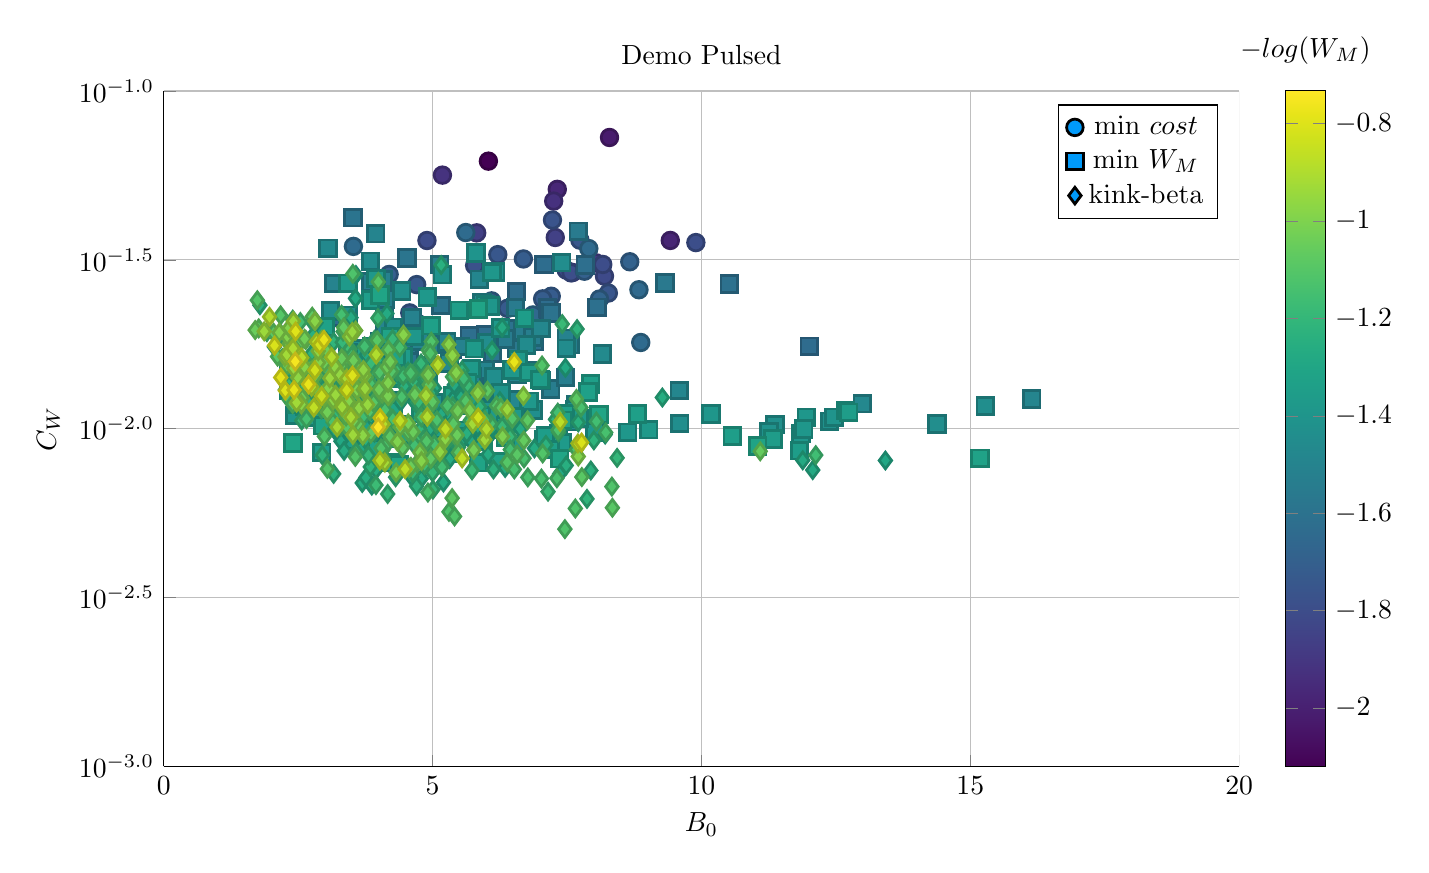
\begin{tikzpicture}[]
\begin{axis}[colorbar = {true}, height = {101.6mm}, ylabel = {${C}_{W}$}, title = {Demo Pulsed}, xmin = {0.0}, xmax = {20.0}, ymax = {0.1}, ymode = {log}, xlabel = {${B}_{0}$}, {unbounded coords=jump, scaled x ticks = false, xticklabel style={rotate = 0}, xmajorgrids = true, xtick = {0.0,5.0,10.0,15.0,20.0}, xticklabels = {0,5,10,15,20}, xtick align = inside, axis lines* = left, scaled y ticks = false, yticklabel style={rotate = 0}, log basis y=10, ymajorgrids = true, ytick = {0.001,0.0031622776601683794,0.01,0.03162277660168379,0.1}, yticklabels = {$10^{-3.0}$,$10^{-2.5}$,$10^{-2.0}$,$10^{-1.5}$,$10^{-1.0}$}, ytick align = inside, axis lines* = left,     xshift = 0.0mm,
    yshift = 0.0mm,
    axis background/.style={fill={rgb,1:red,1.00000000;green,1.00000000;blue,1.00000000}}
, colormap={plots}{rgb=(0.26700400,0.00487400,0.32941500), rgb=(0.27794100,0.05632400,0.38119100), rgb=(0.28291000,0.10539300,0.42690200), rgb=(0.28229000,0.14591200,0.46151000), rgb=(0.27619400,0.19007400,0.49300100), rgb=(0.26514500,0.23295600,0.51659900), rgb=(0.25042500,0.27429000,0.53310300), rgb=(0.23360300,0.31382800,0.54391400), rgb=(0.21813000,0.34743200,0.55003800), rgb=(0.20123900,0.38367000,0.55429400), rgb=(0.18555600,0.41857000,0.55675300), rgb=(0.17117600,0.45253000,0.55796500), rgb=(0.15772900,0.48593200,0.55801300), rgb=(0.14618000,0.51541300,0.55682300), rgb=(0.13374300,0.54853500,0.55354100), rgb=(0.12346300,0.58168700,0.54744500), rgb=(0.11948300,0.61481700,0.53769200), rgb=(0.12632600,0.64410700,0.52531100), rgb=(0.15014800,0.67663100,0.50658900), rgb=(0.19109000,0.70836600,0.48228400), rgb=(0.24607000,0.73891000,0.45202400), rgb=(0.31192500,0.76782200,0.41558600), rgb=(0.37777900,0.79178100,0.37793900), rgb=(0.45867400,0.81636300,0.32972700), rgb=(0.54552400,0.83803900,0.27562600), rgb=(0.63690200,0.85654200,0.21662000), rgb=(0.73088900,0.87191600,0.15602900), rgb=(0.81457600,0.88339300,0.11034700), rgb=(0.90631100,0.89485500,0.09812500), rgb=(0.99324800,0.90615700,0.14393600)}, colorbar style={title=$-log( W_M )$}}, ymin = {0.001}, width = {152.4mm}]\addplot+[scatter, scatter src=explicit, only marks = {true}, color = {rgb,1:red,0.00000000;green,0.60560316;blue,0.97868012},
draw opacity=1,
line width=0,
solid,mark = *,
mark size = 3.0,
mark options = {
    color = {rgb,1:red,0.00000000;green,0.00000000;blue,0.00000000}, draw opacity = 1.0,
    fill = {rgb,1:red,0.00000000;green,0.60560316;blue,0.97868012}, fill opacity = 1,
    line width = 1,
    rotate = 0,
    solid
}] coordinates {
(6.0376291897873084, 0.06197483174638786) [-2.119809409407475]
(8.29014098058992, 0.07282952610606806) [-2.022107373269494]
(9.420103794137964, 0.03609135913093006) [-1.9777667149411715]
(7.318722954994432, 0.051130362720294704) [-1.969913275543008]
(7.25219757869589, 0.047199699242522014) [-1.9276279243167613]
(5.1830212243548095, 0.05634035623848662) [-1.9180907603558137]
(7.605075373452645, 0.0290156978870517) [-1.8866814459155106]
(8.038027414173005, 0.030992141550921816) [-1.8810042714594786]
(5.819960412661949, 0.03801538835634297) [-1.861231108978198]
(7.281484484411212, 0.03683114347875789) [-1.8558362580925096]
(8.196367519793338, 0.028291519575269056) [-1.811508198071671]
(4.895214337316329, 0.03607745072820276) [-1.8048956433290855]
(8.164740419623248, 0.030644555029908985) [-1.797922304180305]
(7.485375190378305, 0.02949537628440487) [-1.7974494679074275]
(7.575835693873996, 0.028933124859920306) [-1.7961193741663348]
(9.896061646161176, 0.03557653455378664) [-1.7922955251500743]
(5.781753762991258, 0.030417392770278703) [-1.7763653379983415]
(7.2293817061271435, 0.04147970255534964) [-1.762574168304495]
(8.268196094729024, 0.025210912703269035) [-1.7524000959584443]
(7.738981336245074, 0.036173737778618126) [-1.7467043012053995]
(6.212564476265189, 0.032766263996239824) [-1.7445197156480476]
(4.575558741192934, 0.02202338694073385) [-1.7362913649987812]
(4.703832637956078, 0.026714074548194577) [-1.7340594740544224]
(6.392336735687798, 0.022713661122324157) [-1.7289223235866222]
(7.206811582654181, 0.02466928657304406) [-1.719614121069955]
(7.047211448521989, 0.024233508820652228) [-1.7167136137505041]
(6.688671457635685, 0.03181143352229567) [-1.7154437116459917]
(4.191978956537718, 0.028622291298276443) [-1.7060722509483957]
(7.823016295826839, 0.02926238447048653) [-1.6937830944780397]
(8.667006322370625, 0.03120868171359675) [-1.6889812321302553]
(6.097668524082785, 0.023905595143656186) [-1.686209077026567]
(8.103448360984764, 0.024204963735087338) [-1.6786883535604935]
(4.743339804248675, 0.020413682949498045) [-1.6734478593396724]
(6.86661111430788, 0.02171708878277083) [-1.650681965327452]
(8.837409416541565, 0.025789595420542006) [-1.6458495153344535]
(7.905189202860984, 0.034141771708853026) [-1.6412636709027566]
(5.617445394262159, 0.03809649700399676) [-1.6393314314904326]
(3.5279604177676442, 0.0346599142742729) [-1.6390302509540549]
(8.87108059531098, 0.018002375584230325) [-1.6381696948341165]
};
\addlegendentry{min $cost$}
\addlegendentry{min $W_M$}
\addlegendentry{kink-beta}
\addplot+[scatter, scatter src=explicit, only marks = {true}, color = {rgb,1:red,0.00000000;green,0.60560316;blue,0.97868012},
draw opacity=1,
line width=0,
solid,mark = square*,
mark size = 3.0,
mark options = {
    color = {rgb,1:red,0.00000000;green,0.00000000;blue,0.00000000}, draw opacity = 1.0,
    fill = {rgb,1:red,0.00000000;green,0.60560316;blue,0.97868012}, fill opacity = 1,
    line width = 1,
    rotate = 0,
    solid
}] coordinates {
(12.006327167234412, 0.017540808339758972) [-1.6348798048481208]
(7.13617498148303, 0.022785258097976623) [-1.6277277898588538]
(7.070736325233126, 0.030625514244526048) [-1.627684330571819]
(6.56017053121773, 0.025489957683783454) [-1.6248467182009472]
(5.980925581195891, 0.0189830433690413) [-1.62256122166559]
(5.681680569563924, 0.018838350678554387) [-1.6197529434592726]
(7.838353199376363, 0.030553347689269015) [-1.619473374550493]
(3.1599502425274832, 0.0213568595963161) [-1.6190205769362032]
(5.370255019403915, 0.017173711360022336) [-1.617478678707941]
(8.057787659408406, 0.022891816741403965) [-1.6135161817566324]
(10.515719243031652, 0.026834336105762403) [-1.6079101518459553]
(6.442976568556264, 0.01976733422078956) [-1.6005797137016178]
(6.892650960552643, 0.01811055755791537) [-1.5991182248913247]
(7.198509347079774, 0.02202289176749285) [-1.595836360479248]
(3.517726346433672, 0.042161103004000076) [-1.589397412964098]
(5.159769580238814, 0.0231728109038665) [-1.589205111302375]
(3.8365890735140322, 0.015450272567257462) [-1.5875377953010883]
(4.522678122476023, 0.0319953061173649) [-1.5845809864087244]
(4.56749863701147, 0.016164039710660088) [-1.5775674018565111]
(6.114630190971535, 0.016693759971981265) [-1.5713155071601692]
(6.555603899680141, 0.01726409176752251) [-1.5652457853616617]
(9.324368979144754, 0.02698353416604086) [-1.5643952661253622]
(4.546856339243231, 0.01769761001811183) [-1.5595601870169422]
(6.5407531731873325, 0.02281153437267921) [-1.552568848396255]
(7.709084001143297, 0.038423068705951594) [-1.5520441226990631]
(4.10568363851079, 0.022224095489930037) [-1.544925041354305]
(6.355103453558186, 0.01841847429182733) [-1.5430023738862098]
(6.679865116269665, 0.019477644457703495) [-1.5396243114452017]
(4.896210634322484, 0.01449908817629988) [-1.538692217528126]
(7.198003119281151, 0.013092644307368572) [-1.5373740781698282]
(5.131173117670862, 0.030574977212997605) [-1.5350312948909135]
(7.472740510067807, 0.014205258889817484) [-1.5317433014682034]
(6.8683725940871865, 0.018689708848548738) [-1.5311850486265117]
(5.766565183000099, 0.01387590038164943) [-1.5287451237254033]
(5.73965239781306, 0.013905952265261586) [-1.526526816139614]
(3.850247344392022, 0.027241135712482305) [-1.519178921439465]
(3.724681151757905, 0.016910779414334946) [-1.517891032933806]
(4.124143130105857, 0.024191852864153648) [-1.5130165343032327]
(7.561125230807454, 0.01773125993862434) [-1.5126055054907948]
(4.0802413603524945, 0.027530426264504002) [-1.5122759735909235]
(6.754598599599373, 0.014899481481132758) [-1.5121531835443067]
(5.140825889424527, 0.01778122202031051) [-1.5121518481580156]
(7.487694805484361, 0.01852162588841651) [-1.509963665969106]
(4.706543051446386, 0.013259386458548635) [-1.5098191352881933]
(4.023530685620901, 0.018078145365757758) [-1.5094600237705913]
(4.619206299311601, 0.02134336001409843) [-1.5091677016781566]
(5.515733266875538, 0.017507453096671365) [-1.505813383704145]
(3.1665229051711936, 0.026909424888676328) [-1.5035180904231982]
(4.7606297434625375, 0.018116695499993292) [-1.4998070828001184]
(2.6908911342489987, 0.01226652304303364) [-1.4993412700061268]
(5.9813285749518785, 0.014898889997617197) [-1.4970388348465338]
(5.73832856833363, 0.014279317114283529) [-1.4968151314329754]
(3.9410419383640107, 0.03778412752723575) [-1.4959262215207656]
(3.430490492055365, 0.012007443130458324) [-1.495878750102406]
(3.3992707879943804, 0.014131383104205364) [-1.4911760171512294]
(3.8869352833553514, 0.013847785437885679) [-1.4909012021072667]
(3.492353905872561, 0.013113327535403696) [-1.4904727997922445]
(16.140534236107158, 0.012253217681920671) [-1.4902975254497872]
(4.106645540108447, 0.020179920200301855) [-1.4899596862430686]
(6.569539440995961, 0.014465480638895564) [-1.484315053758591]
(9.588346294205625, 0.012974868808400592) [-1.4832272441818983]
(5.870682126151471, 0.02767164571202513) [-1.481908947186888]
(3.925275118526448, 0.012700241486954703) [-1.481610811848838]
(5.262489226894273, 0.018066556725317685) [-1.4808315890609627]
(5.861692393922073, 0.012152582495637852) [-1.4803924190961808]
(5.918313590579109, 0.023591043628319753) [-1.4777813991456452]
(3.8833429023200345, 0.014987126189756067) [-1.476226145125234]
(6.481366220083333, 0.012179602718049342) [-1.476103765156545]
(7.019026450980214, 0.0198044997246676) [-1.4759532635696884]
(12.992560883586702, 0.011854698849849837) [-1.4744693843941874]
(5.3126270403520905, 0.015665176708494814) [-1.4721189566530006]
(4.653270023129369, 0.012892988065699775) [-1.4694765884704042]
(5.56336817143885, 0.011723605612914264) [-1.4684762544315009]
(5.887370453127917, 0.01146148363735155) [-1.4673712598422484]
(4.769173324013478, 0.01403086783418577) [-1.4665127712450712]
(3.0555463671233567, 0.03422172209265897) [-1.466465342676487]
(7.658132277548963, 0.011814056076879775) [-1.4656409913573911]
(8.15735419014013, 0.01666169164744686) [-1.4607639902508311]
(3.6997605874700903, 0.011797068547740396) [-1.454804800167485]
(6.7465287199750925, 0.017714850999176746) [-1.454016548396377]
(7.488515154319888, 0.01730924236440855) [-1.449126660054787]
(4.899466318563284, 0.015350811156516968) [-1.4450317564339483]
(7.901350621283068, 0.010700521525178483) [-1.4442476160174416]
(6.002415704010382, 0.017999193081243068) [-1.4428695943470562]
(3.846424137063846, 0.03129913412451443) [-1.4416527786165851]
(7.401783272746636, 0.030992801350489627) [-1.4412978501823663]
(7.020304767734094, 0.013876797144792313) [-1.4410674847520173]
(14.381919368485658, 0.0103371343106061) [-1.4407593364531412]
(3.1028814474410384, 0.022291694526716137) [-1.4382523340904476]
(3.7705732972432857, 0.011033535668865918) [-1.4374618391296154]
(5.967712362691083, 0.011578760205733224) [-1.437309497392895]
(6.135496498952566, 0.014225493350487712) [-1.437004502630189]
(15.280361971651645, 0.011662685993065088) [-1.4369516286418977]
(9.595768152006077, 0.010363517857158673) [-1.4359296968945898]
(2.706516860566676, 0.012593943496598788) [-1.4348111698815942]
(7.531253395446069, 0.010486068251726523) [-1.4347403934029699]
(6.873696165627944, 0.011351647420548932) [-1.432162507533083]
(6.006312634325258, 0.010703895251080882) [-1.4298959659652046]
(11.369550336874795, 0.010279170294604838) [-1.429141349371285]
(4.426279201300683, 0.025557043779995653) [-1.4288294492620477]
(4.273188204709541, 0.019981046165081038) [-1.4275892047251812]
(3.284854781128933, 0.014011150106021747) [-1.42664672926539]
(3.563101077929043, 0.017276630179413652) [-1.4239039330716527]
(7.65153347612068, 0.01135063897630595) [-1.4237047673472223]
(3.427537242139707, 0.021651736693319764) [-1.4220880228019461]
(6.174362312871966, 0.029124606257697153) [-1.4214589216983458]
(12.38255150794347, 0.010524080735331771) [-1.4192750546166355]
(3.96419825273711, 0.012152497168515361) [-1.4188846212567885]
(4.984822443753677, 0.010654264771940928) [-1.418142111238707]
(4.177511278387798, 0.012093014306414056) [-1.4175771687309422]
(4.494983202230982, 0.010307835186267926) [-1.4166515403180218]
(11.258702848316975, 0.009802839106844477) [-1.4151591623618127]
(4.167168689552534, 0.012089411129630757) [-1.415086999740124]
(3.4268121903746978, 0.016771907819218872) [-1.4150518254702726]
(2.3537099631543916, 0.01479570625667246) [-1.412750376425469]
(5.182420388292304, 0.02858609969916251) [-1.4118418857799215]
(3.927997304454704, 0.009976658176736495) [-1.411745253778192]
(5.018593701573295, 0.011899859669740264) [-1.4101129990450592]
(3.885531120492574, 0.010975696046095008) [-1.4098064292280077]
(5.2474162565909435, 0.010078193568331789) [-1.4071217370506766]
(6.2004105061477235, 0.012567870805096065) [-1.4069653518342513]
(12.464033848113864, 0.010809590548122633) [-1.4053188021751997]
(3.762648000098064, 0.013228123351848638) [-1.4040831795581317]
(3.7635564019241006, 0.012756284815624411) [-1.403783408224447]
(6.2439977027647595, 0.011849909135487101) [-1.4034059706684434]
(4.011269493628918, 0.015391572104901911) [-1.4031334212883295]
(5.948372401188327, 0.011370525417095621) [-1.4027031557706915]
(6.105240096014571, 0.010883116023126084) [-1.4023409214316394]
(5.807785740293634, 0.03314304390232683) [-1.4018234466267534]
(6.240369813761391, 0.010943279854872806) [-1.4001967788421508]
(6.270554586884656, 0.012776602146795163) [-1.3983213447403338]
(10.178788051574003, 0.011065372696240975) [-1.3946316971345938]
(7.342798909437036, 0.009697674748088487) [-1.393981306323598]
(5.515659388841616, 0.012316212001497684) [-1.3939743444895971]
(5.981611630666005, 0.023293627402023516) [-1.3938659098694006]
(3.371060773893557, 0.012799262525216688) [-1.3934317035795]
(6.064709438936184, 0.02306752096780418) [-1.3919378361313393]
(2.855332574063217, 0.011575943181240602) [-1.3913501343623875]
(2.4437405695506387, 0.010938935413839007) [-1.3899986150261634]
(6.469695877217161, 0.014916276865219583) [-1.3888953225499234]
(11.950718647766315, 0.010811642128190005) [-1.3883849558567678]
(5.747775187553233, 0.012086573842968483) [-1.3880683151937296]
(8.62770676217042, 0.00974951527611275) [-1.3879257169733152]
(4.661434120932319, 0.01875474559032549) [-1.387200255154835]
(6.101706649362307, 0.028992717747430105) [-1.3869139374162498]
(4.921653466094031, 0.014275341697562267) [-1.385982080919773]
(11.85196051673142, 0.009658736241223327) [-1.385951966541943]
(11.902146743793873, 0.009979205376142167) [-1.384341496966052]
(8.017011891149473, 0.009781750047901397) [-1.3836628266676982]
(3.9453588859348705, 0.027837899406166513) [-1.383138617240496]
(2.7450573045264335, 0.013692957043690078) [-1.3831333668949872]
(6.793555399638037, 0.012055028195149642) [-1.3823755173012382]
(4.903012581972081, 0.02457168150365556) [-1.381386436684111]
(3.8233047461789904, 0.013467436970042478) [-1.381013926041926]
(3.9360749856112256, 0.01632900764605371) [-1.3807582017142732]
(4.3204944514848105, 0.016233342907168043) [-1.3795912650626003]
(6.26763114858317, 0.019856726760879642) [-1.3784744825946547]
(9.017994817618085, 0.009937020814786353) [-1.3784050115817357]
(5.662871931648498, 0.012947457233964572) [-1.3727350903904059]
(3.423561741004342, 0.02692798924274793) [-1.3726382795387042]
(6.527451391525709, 0.00894061047284123) [-1.3726183217257064]
(6.511799045245276, 0.01083618948017438) [-1.370506635821487]
(6.061861020595905, 0.010820381028973857) [-1.3702834841058706]
(5.720454003557526, 0.01507474130083674) [-1.3699905172740252]
(6.595551058907596, 0.016024901755414496) [-1.3694510931398833]
(7.0656961487120595, 0.009286958803152093) [-1.3690194932725448]
(5.7756989121996005, 0.01725165686414962) [-1.3685993689556193]
(7.407124185747266, 0.009100422809121853) [-1.3680782620249432]
(5.940087524048422, 0.009358898748733285) [-1.3659937757563743]
(7.721929512311208, 0.010741593794976297) [-1.3655266043175585]
(4.375024347794328, 0.00935804014953258) [-1.365489135635999]
(4.45788760453061, 0.01631624677926724) [-1.365314944668722]
(12.678530079731434, 0.011316654652064283) [-1.3620488306806053]
(2.8403626573133516, 0.010811158792461435) [-1.3600883836878876]
(6.791476575808721, 0.014663988794896813) [-1.3569999482959285]
(11.332959766691456, 0.009327975573933072) [-1.3565369493574833]
(3.5993697558328135, 0.009591330831744169) [-1.3564434514013937]
(7.094333669876596, 0.009510520762087537) [-1.355670949654743]
(11.824184374151493, 0.008600603815848054) [-1.3550689180362785]
(6.708017904184935, 0.0212306523206366) [-1.3545717493575382]
(3.9462715514882833, 0.011027495783414606) [-1.3536406793714741]
(3.846707059253749, 0.02403578580290836) [-1.3522480304376618]
(5.54278675314685, 0.01277987363566607) [-1.351683168790268]
(12.739777598462709, 0.011181317227288103) [-1.3509416538039447]
(6.996720111065061, 0.013988110662625983) [-1.350917699634303]
(5.58993729043943, 0.011706003302806382) [-1.3498675794038522]
(3.872376016258126, 0.01744787935363008) [-1.3480954361555229]
(10.572844829384726, 0.009513333911267541) [-1.3474307155472665]
(2.938257234568377, 0.008506399274340092) [-1.345835600508895]
(5.495169200054534, 0.022402494346273383) [-1.3441619287129023]
(3.5507214607316238, 0.011568935524735228) [-1.343173024895477]
(5.504907463368559, 0.009888039453025594) [-1.3431102335422052]
(5.65163629087646, 0.013676025720795522) [-1.3418959513921676]
(7.466637754651223, 0.011055478792069253) [-1.3416390955818198]
(7.940566023194332, 0.013562184857025608) [-1.3412225668983788]
(4.645128912048539, 0.013928329166195007) [-1.3411223781363122]
(3.5178351993254204, 0.008957609956171385) [-1.3409980727589041]
(8.80912527255541, 0.011061155580644737) [-1.3407774046291352]
(4.414263871815846, 0.014142372730384274) [-1.340736718067575]
(3.5324039876905395, 0.014931289500105476) [-1.340172101894623]
(7.191161190692271, 0.008673821452175847) [-1.339371225527388]
(7.889566195214564, 0.012851757813003692) [-1.3355889626958743]
(5.053734570947225, 0.009585198585080813) [-1.3353537500446666]
(3.197632928999906, 0.011502571386254939) [-1.3352936153265889]
(4.973690447707013, 0.020177908654106694) [-1.3347167954999664]
(5.902248798024801, 0.010934192827515073) [-1.3333464153994234]
(6.352797677366824, 0.010187040046408826) [-1.3319467069356516]
(5.715498297799574, 0.012093243108414115) [-1.3317606682979195]
(6.242863088777295, 0.0099544891977854) [-1.330878268232421]
(5.056377266744529, 0.00892167491417854) [-1.329838199225075]
(3.0039565360029306, 0.020024514359414238) [-1.3275817805394716]
(3.774870490274173, 0.010377685225384297) [-1.3271981479523673]
(3.4560894708307504, 0.00923521460571462) [-1.3257753666633474]
(3.739062356737302, 0.016536435428404248) [-1.324805801675252]
(15.176586722658566, 0.008177838551829547) [-1.3236480395933032]
(3.419819319784293, 0.01320289357034274) [-1.3223872875360454]
(6.352130677917973, 0.009416665871049234) [-1.320790714548859]
(2.322477510691322, 0.012966997564871513) [-1.3198610091294973]
(2.324248942944489, 0.014941915896507264) [-1.3173999901029887]
(4.846244775501472, 0.014705731648914599) [-1.3172398911361078]
(4.214745039825576, 0.018745840734049092) [-1.3155841266914403]
(11.045339988929378, 0.008883845818604448) [-1.3144429555765318]
(4.3255410851853195, 0.016334708642476756) [-1.3140984246311314]
(6.235375099026929, 0.007999169369094802) [-1.3136141988883636]
(7.418567204666788, 0.010593671042148305) [-1.3130409307938926]
(3.522574707719547, 0.011696426000066894) [-1.312883593567563]
(5.395063115984087, 0.008437215022084032) [-1.3113636666391015]
(2.9623590695188793, 0.010210442889078589) [-1.3110543205827916]
(2.619151065722938, 0.01161135507437133) [-1.3101666476591896]
(4.251202424158484, 0.010715857251244127) [-1.3094281744638252]
(5.850851943214601, 0.007935513211517508) [-1.3092819198295769]
(2.800331008488367, 0.01527961135499392) [-1.3091789421820008]
(3.962750439094108, 0.008718673720708605) [-1.308657609117127]
(3.9491153183500765, 0.012115862676003172) [-1.30815684782275]
(5.368732790803233, 0.012528702800938256) [-1.3073192126014976]
(5.531029878673032, 0.009466859805614364) [-1.306104667504652]
(4.019577892699671, 0.024862203238592617) [-1.3061029424340123]
(5.854899512854821, 0.022588731344076834) [-1.3059932173472433]
(3.4111150555142538, 0.010067194372351543) [-1.3053424100316993]
(5.9474935100169155, 0.009194414774426339) [-1.3048906180553326]
(4.442986113810117, 0.014224364223609164) [-1.3043596581137094]
(4.484605690017701, 0.00966642720928779) [-1.304157201921016]
(4.235072291257464, 0.007934056288357859) [-1.3040523349428945]
(2.481542761360737, 0.011830250137913223) [-1.3039439069452712]
(7.36295762251903, 0.008152912507864905) [-1.3022467953572583]
(4.272648359589559, 0.011323662495891916) [-1.3012176243848619]
(2.403751630196505, 0.009074217857747638) [-1.3011866801418175]
(8.097817905088668, 0.011011974496683653) [-1.3004916659282275]
(4.379478185125185, 0.007824745570931163) [-1.3001880033121107]
(4.787155359091795, 0.011078402389842862) [-1.2993649239636758]
};
\addlegendentry{min $cost$}
\addlegendentry{min $W_M$}
\addlegendentry{kink-beta}
\addplot+[scatter, scatter src=explicit, only marks = {true}, color = {rgb,1:red,0.00000000;green,0.60560316;blue,0.97868012},
draw opacity=1,
line width=0,
solid,mark = diamond*,
mark size = 3.0,
mark options = {
    color = {rgb,1:red,0.00000000;green,0.00000000;blue,0.00000000}, draw opacity = 1.0,
    fill = {rgb,1:red,0.00000000;green,0.60560316;blue,0.97868012}, fill opacity = 1,
    line width = 1,
    rotate = 0,
    solid
}] coordinates {
(3.5121202416558273, 0.012133883145293747) [-1.2971735267311564]
(5.277662377204398, 0.008497507185750146) [-1.2963451470925318]
(4.933311521981375, 0.011968595839803002) [-1.2939289874566402]
(13.420827419108324, 0.008051203599652048) [-1.2928570974581939]
(5.71174352009151, 0.009198462479520332) [-1.2926592596370523]
(5.012096245785827, 0.009976448637174172) [-1.2918359622137705]
(3.8248114438663654, 0.011200517330116096) [-1.2901565279273088]
(2.959247673493197, 0.014778677283745992) [-1.2885231243501492]
(4.219667355934983, 0.009645840422057206) [-1.2873870680148987]
(3.9368699206088387, 0.015368153744705897) [-1.2867189599495152]
(5.3763072490644115, 0.012200186404574626) [-1.2866608738447551]
(6.009303119414782, 0.009314200607444962) [-1.2862989627940875]
(7.363118579080014, 0.007351086075188858) [-1.2856479743658245]
(4.035860790767533, 0.011184811263709776) [-1.283461572944208]
(3.5737740510711875, 0.028511756618296732) [-1.282628142229196]
(3.295672492906566, 0.0091809969411667) [-1.282318795548118]
(7.469892811394071, 0.015147418693115068) [-1.2809419797501462]
(3.716712298492769, 0.009441743395354373) [-1.2802239523296417]
(5.842646483303914, 0.010115067051441084) [-1.279661807174519]
(3.655882587201946, 0.008682653521467484) [-1.2793586996677089]
(5.000424842433475, 0.00919694313697991) [-1.279241431080542]
(11.883710143751259, 0.008062649665833432) [-1.2791738597664242]
(3.769661149622435, 0.016537125137685977) [-1.2777724695025643]
(3.565755959498115, 0.024311609583825906) [-1.2776560252665474]
(12.069034139998493, 0.007543708329813699) [-1.2776226586446298]
(5.402872542958727, 0.013472425466080754) [-1.2772080908839465]
(3.5721530790668217, 0.010591022499429533) [-1.2768888641183538]
(6.113391779890812, 0.010068814155906535) [-1.2749252706301877]
(5.281892154588248, 0.011122028940902477) [-1.27405635520294]
(2.8318856035975837, 0.020592443763116842) [-1.273999627133777]
(3.171270658752047, 0.009932693135460512) [-1.2739263340884897]
(5.035138050414791, 0.013177764718534145) [-1.273686836355838]
(4.151495259485247, 0.021930543698997433) [-1.272060671091855]
(3.9079897018955214, 0.01703366147805158) [-1.2717552020206426]
(3.0490838025892786, 0.013199694993892157) [-1.2715552113887816]
(3.026643094075235, 0.018137179053328113) [-1.2711256143593725]
(5.509559307824704, 0.009089213335736035) [-1.2706918059143955]
(6.2933025717891, 0.019922160606497104) [-1.270659241243097]
(8.209845211268025, 0.009612072783370788) [-1.2706266042708976]
(2.738511903007871, 0.011815687417752718) [-1.2699973230973551]
(5.3168436208878225, 0.008127375094877596) [-1.2694883213650459]
(3.8713710824000858, 0.011108460101523684) [-1.269469949244091]
(4.40489854224676, 0.01200413289507089) [-1.2693810054133523]
(3.4817589149659844, 0.021322131632939743) [-1.2685038799823198]
(6.893437951158227, 0.008746022086925008) [-1.268011220133286]
(6.250792601428729, 0.012071261699451271) [-1.2676767161765092]
(3.8480774904528383, 0.015027760071695463) [-1.2672360183442966]
(5.528072317285266, 0.012386782250268949) [-1.2670329245716005]
(6.631542703995221, 0.00997135774995843) [-1.266521603924258]
(3.402074742995083, 0.014743359804979298) [-1.265829536383991]
(5.157191379781698, 0.011015221663609409) [-1.2655850749955841]
(4.081908569510066, 0.009754591610171831) [-1.2651606387913807]
(6.032688069883985, 0.008391084675782472) [-1.2650267302153226]
(6.323926257057424, 0.011459660264397842) [-1.2643165163116283]
(5.673390538312956, 0.01314380020899071) [-1.2638630587832318]
(4.962600203221328, 0.0100188505842072) [-1.263682663264664]
(5.202158247710273, 0.006930908540990179) [-1.2635507051033026]
(6.3498106860494135, 0.007655768190498255) [-1.2630930817893484]
(3.3542410941806997, 0.008595102325139414) [-1.2620028969039807]
(5.408801595842229, 0.008993269936185943) [-1.2617711256664215]
(4.060468748765856, 0.013435175267701598) [-1.2607622270815175]
(4.3458863312043015, 0.010399130132164968) [-1.2599969566754825]
(4.941827638049582, 0.011066872440514844) [-1.2580199333772297]
(3.7865968807980463, 0.014164623239439114) [-1.257674742909116]
(3.8700982106168342, 0.006784814729690784) [-1.256920205986828]
(3.860117954844053, 0.010847484174753686) [-1.2558826127376497]
(4.667259329944255, 0.012006910499828622) [-1.2545784323742915]
(9.273036766388604, 0.012367303307791636) [-1.2541769145790829]
(3.6923348872456994, 0.006909773766752695) [-1.2538081670568602]
(4.789726542521002, 0.007118806510545466) [-1.2537331036632384]
(3.7600070371379886, 0.007163920014099904) [-1.2523947287534352]
(4.421298005693511, 0.01409766195530951) [-1.252161894882265]
(4.610630866671953, 0.007191926525759095) [-1.2517841257242934]
(5.20128149593585, 0.010140660180167243) [-1.2510148685101052]
(4.053725242509742, 0.009947685467565285) [-1.2503817284236358]
(3.9490509942400003, 0.00755783116205777) [-1.2500618007814928]
(6.105587908907182, 0.01705584468677382) [-1.249408930050928]
(7.485181266118961, 0.007782048369656626) [-1.248434923528094]
(5.429695722081377, 0.009638865392082259) [-1.246475793101881]
(5.6359771653268504, 0.009668090359024908) [-1.2453083223674235]
(3.585647465370671, 0.01181801423349667) [-1.2430271033455136]
(4.967782040145293, 0.012765537294567253) [-1.2425009663963265]
(2.836991692259108, 0.014096920088512531) [-1.2420036959161107]
(3.851942066673645, 0.014638041989732616) [-1.2406291651922927]
(3.86783106759803, 0.011330221246013529) [-1.2404081246835275]
(4.144235850020982, 0.009882346466549934) [-1.2402721066912186]
(5.159714665590853, 0.030517882462548936) [-1.2399829928026451]
(2.7744066236166, 0.018855374361929193) [-1.2398403601837327]
(2.9616080503895255, 0.013105067185166342) [-1.2382227382575577]
(1.789190176158448, 0.023206171452307512) [-1.2372685823332665]
(2.057072816922599, 0.01748239328622686) [-1.2369979991721363]
(7.709371728502172, 0.010436966421480154) [-1.2364971528125899]
(3.754765214297292, 0.00929031971105747) [-1.235918342000411]
(2.4390459870956867, 0.01224311754662533) [-1.235332112263366]
(4.477287158856502, 0.013377000135851953) [-1.235230354209212]
(7.942543848452732, 0.00752176857171885) [-1.2348662947331168]
(6.132444327284232, 0.007577390318458053) [-1.2331237451825037]
(7.107404657748289, 0.008954934736687754) [-1.2314216648450123]
(3.1603738338503238, 0.007348723496235854) [-1.2276908244938955]
(4.701751679050523, 0.00675688814735783) [-1.2234874983546444]
(3.1402652758611795, 0.01611655322423877) [-1.2224132121245386]
(7.999091158540905, 0.009234491873309686) [-1.2212129344183997]
(3.445549117779653, 0.012691970303684906) [-1.221000044288545]
(3.3885426284661953, 0.011032294768272291) [-1.2201668573985105]
(5.5456091712090725, 0.014875616723151944) [-1.2200113852982524]
(4.54243872092666, 0.014755597501979523) [-1.2200110437170943]
(2.4705292036298423, 0.015480160187022769) [-1.2199386530853975]
(7.687093361817087, 0.019725018407248666) [-1.2192027637421239]
(3.3454463511646835, 0.01227428321856098) [-1.218844626416703]
(2.8137615251130303, 0.013727476887235461) [-1.2187513907488479]
(4.312486225133877, 0.007184219051293641) [-1.2182120816961266]
(4.772997377730909, 0.011425165896800414) [-1.2178523450390264]
(2.7578042878780122, 0.01671459075301228) [-1.217564445140848]
(3.8197074658287047, 0.01316079396243774) [-1.2148287908302686]
(7.285303183831831, 0.010653867811546877) [-1.2144650329368094]
(7.87104962823073, 0.006198307301760009) [-1.2142295699793069]
(3.9206245950101466, 0.009725241928162248) [-1.2114971471794018]
(2.949515743068061, 0.00834877000609595) [-1.2110590840755884]
(6.340610180985918, 0.010394495894857034) [-1.210956786812969]
(5.875295019857379, 0.01160689504064373) [-1.210625479626572]
(3.8412979296256804, 0.007709496307162327) [-1.210548450407708]
(4.861863097960495, 0.01196700634860152) [-1.2101072964851303]
(3.685725743106405, 0.014267222031421351) [-1.2097043828037173]
(3.0450965804813084, 0.017649120721508472) [-1.2090548152300868]
(5.178245200408863, 0.00786922573538261) [-1.2089432452477198]
(3.1609089410843576, 0.018050177035811292) [-1.2088567702310062]
(4.648811455834014, 0.01374396978202603) [-1.208355792529063]
(2.6748681285923954, 0.012119563498851512) [-1.2079597098695036]
(3.4809700733273528, 0.01476620759208673) [-1.2069143247822283]
(2.5693210089699696, 0.014425121215984256) [-1.2060355587049236]
(5.48357638584481, 0.008818373193963157) [-1.2051439881244612]
(3.5314903256684156, 0.014347196234709005) [-1.2048202874468241]
(2.7372435536225725, 0.013090961135950088) [-1.20412102013171]
(8.431693660708335, 0.008195788944222735) [-1.2006084749599055]
(3.22168634343002, 0.011017845567179161) [-1.1997509076464346]
(2.71871093880185, 0.01471498897475931) [-1.1989561148134826]
(2.566609676009112, 0.010576750792174504) [-1.1977552093777106]
(3.976434539417637, 0.015955953274896677) [-1.1973464324024234]
(4.873125471162229, 0.014024797653122234) [-1.1952843257986516]
(4.765913327506254, 0.009913142251828634) [-1.194608172565493]
(4.100942713127369, 0.012231614304186931) [-1.1943983553124515]
(3.211186770718166, 0.012895825589119291) [-1.1943709063726027]
(3.8064949992758947, 0.008341248647504823) [-1.193465520169887]
(5.000301151056601, 0.007422215660710276) [-1.1934529196767811]
(3.320155156974005, 0.018029259293378272) [-1.1932608414538086]
(3.75169525130439, 0.01475503745943627) [-1.1930245850534404]
(4.785428924434849, 0.01559839957452813) [-1.19275308105931]
(5.006411779829835, 0.006601321305241876) [-1.1925650410586528]
(4.729161558851959, 0.012849471675853265) [-1.1916847830033912]
(4.164290783750659, 0.006406786662781295) [-1.1906829642457115]
(3.8087569173433318, 0.015231829402577652) [-1.1905171502567853]
(4.25698051374954, 0.018424630927819426) [-1.1868792227109848]
(3.5466435162495946, 0.012087057868798792) [-1.1860893620286155]
(5.358611559304756, 0.016048418150957987) [-1.1858875370196502]
(4.738906273187223, 0.011972397837837176) [-1.1854558952607928]
(2.328150699298343, 0.013483711604703155) [-1.1848213366225184]
(3.6344930189881155, 0.011761816070313931) [-1.1847475832442582]
(4.630903293878455, 0.007399398212169979) [-1.1837916630431773]
(3.5912206702417406, 0.010413257435217902) [-1.1834175022102877]
(6.439604151254825, 0.009470444499328991) [-1.1831305353511883]
(3.8587290599416177, 0.015647472969860403) [-1.1828511911535706]
(7.410839889439496, 0.020407456319850734) [-1.181840770808167]
(7.14687725893768, 0.006510208938595967) [-1.1814651012301538]
(6.293989671314393, 0.010147346100150811) [-1.1809344434678004]
(5.074144294813995, 0.010306295906351105) [-1.1788261142099545]
(7.342502353808642, 0.00975845363999315) [-1.1783873972417303]
(3.983645541941601, 0.021255557406142055) [-1.1773891261145735]
(5.733227859571759, 0.007530050850229014) [-1.1772489110999693]
(4.863020029854074, 0.008856286376022381) [-1.1771937197283155]
(2.752607478621478, 0.02079595788529988) [-1.1768483795316644]
(4.34034532964977, 0.01477464262853022) [-1.1754670828809672]
(5.651026413557157, 0.013447350775475101) [-1.1748259721272571]
(3.5729145749442672, 0.008533818365309384) [-1.1743579362801864]
(4.828275081463438, 0.00926629982316415) [-1.1731424023398116]
(5.256321718375727, 0.009127162071787865) [-1.1728411497954707]
(3.9468845539429505, 0.006808109484569134) [-1.172547785671985]
(3.524962730858139, 0.009974514104150454) [-1.171293732602548]
(2.4431003187410245, 0.014894587057756483) [-1.1706435645347975]
(3.366739715078965, 0.014934801738779929) [-1.1704804143126533]
(3.919159617305408, 0.018312728464608994) [-1.1694340492000508]
(3.985672010289093, 0.013038425730797958) [-1.1664836698360914]
(3.9602939466659524, 0.011350876468389677) [-1.166021933665907]
(5.57816396320116, 0.014066615859663486) [-1.1653547583030963]
(3.7135886044363273, 0.01085952514652926) [-1.1637013339225117]
(3.732292225677101, 0.013377410828925157) [-1.1629231949973953]
(2.810904316594346, 0.013971916288186385) [-1.1625677338545028]
(3.034206239153093, 0.01498663044146402) [-1.1615160270969884]
(3.928029894091704, 0.011904820041118874) [-1.1613847421954753]
(2.6232376070221903, 0.013362365525672213) [-1.161380763910868]
(2.181980964430949, 0.019049310191542535) [-1.1612715538980343]
(3.2907142155592495, 0.010122141818818486) [-1.1608808882180581]
(5.371075061307033, 0.011629604231527799) [-1.1602959592128257]
(4.087463063508947, 0.008169777889897055) [-1.1601187846950554]
(12.12505747378403, 0.00834966465898116) [-1.1597072302883453]
(4.633851247354028, 0.014522157751088465) [-1.1596295654776811]
(4.45330922540737, 0.014324434384547807) [-1.1584930595938716]
(4.978980932820263, 0.008145962416336265) [-1.1583013384515075]
(4.072239550506503, 0.008646050418225202) [-1.1578217536561153]
(4.85035182175716, 0.007816314398845932) [-1.1564044749404534]
(4.69723552523336, 0.009241849076330648) [-1.1562110876559482]
(5.176056215218096, 0.007695271029389756) [-1.1558406723410226]
(2.324733000713789, 0.015939165384127457) [-1.1551976368183803]
(8.046084775778542, 0.010505037613581628) [-1.1547723960660046]
(3.463079612931359, 0.01720072822154318) [-1.1547042721803664]
(4.667433759545879, 0.008918107308299703) [-1.1544971334332936]
(7.328473923137891, 0.011156083675037292) [-1.1514583143146417]
(2.3995830140586842, 0.021035989307587558) [-1.150606587165903]
(3.735684839444669, 0.017520815218592205) [-1.1497568820513546]
(1.9186754281020504, 0.019315926185319167) [-1.1488471764736738]
(3.495720099796872, 0.016442878704583205) [-1.14854127278881]
(3.3507099367400888, 0.0147653907680726) [-1.1481443824350337]
(2.5403709550525817, 0.02069244645197561) [-1.1475056240535222]
(3.307281211177642, 0.021750535713550727) [-1.147314943378139]
(2.9349707147715516, 0.011413531346774588) [-1.1452162507505037]
(4.961675340508142, 0.011657490769208391) [-1.1440985305669964]
(6.445744456978382, 0.008671087589979474) [-1.143892607737901]
(5.031670650768643, 0.008990361186615302) [-1.1425154271844815]
(3.2137147299766298, 0.012558201977665608) [-1.1419282223298928]
(5.70066075923312, 0.010576229210216307) [-1.1414111342865825]
(4.790896832026144, 0.010807673225691976) [-1.1409606377195203]
(6.081644185908986, 0.010350872866134037) [-1.140632380055554]
(4.262584437785491, 0.010685556097930418) [-1.1405059694207205]
(2.655348617855336, 0.010680444710790922) [-1.1402761489506106]
(4.884538532888361, 0.01443507208815689) [-1.1390460916159142]
(6.52011178404498, 0.007579718089160525) [-1.1390342976608838]
(8.219749035826943, 0.009743368571375198) [-1.1383859727853913]
(7.7593463773798765, 0.011556690979889052) [-1.1378233474839952]
(4.388904498390582, 0.01739508549026366) [-1.1377132966757475]
(2.87524697467844, 0.011726874929476301) [-1.1376503199229564]
(7.024157829306849, 0.007116540390245059) [-1.1370921105287648]
(3.8400502604153073, 0.013630883580602493) [-1.136359546149739]
(2.4136732196953496, 0.01526251681202216) [-1.1362968805162]
(3.335636087343369, 0.019391120833403556) [-1.1358988321292471]
(3.77790333569627, 0.011860427509089479) [-1.1358539207185072]
(6.699557534343957, 0.008170611753766615) [-1.1356493088623822]
(6.7708197765220905, 0.007176648981252689) [-1.1354932328782563]
(7.311852681214439, 0.007134995489417047) [-1.1335001124055868]
(4.114267644468652, 0.011362840629455528) [-1.1323762690185122]
(4.590968546060674, 0.014605309967466338) [-1.1314565774222176]
(2.262672175094441, 0.013041177771875015) [-1.1310401855629826]
(4.912560401468473, 0.006470994712702174) [-1.130758874865596]
(4.425797376165855, 0.01241454353087534) [-1.1307392487451149]
(5.276947328747049, 0.011706749993287805) [-1.129690412643984]
(5.081053708467179, 0.01058602765458819) [-1.1289684185709847]
(3.1092112052594736, 0.016110870179123358) [-1.128250192514324]
(3.9460119406257674, 0.012109336313631335) [-1.1252475037678356]
(4.11423481085022, 0.008853551975990904) [-1.1245713568718563]
(7.673924172524263, 0.008673362533302236) [-1.1245104109679405]
(3.148239982482193, 0.010444270942938963) [-1.1242443075431308]
(7.332926397268772, 0.009907337069737673) [-1.1228938533825863]
(2.2060310557580083, 0.01617284927660436) [-1.1226570193988834]
(5.971667930097295, 0.010615516830489545) [-1.1219052279962924]
(3.51663552302443, 0.028747991383312018) [-1.1209037456306452]
(4.076712007747793, 0.012621272074607764) [-1.1208704370485616]
(5.3703261256374555, 0.014241574824224812) [-1.1207611585447455]
(3.9821638371433923, 0.018202292531005245) [-1.1203998091578635]
(2.834794233096108, 0.015435434654215487) [-1.1196814354947495]
(2.3348428892798987, 0.012169534423588058) [-1.117569159173303]
(7.460329569062209, 0.0050427739927004075) [-1.1174068253287153]
(8.334229534807674, 0.006738702814170826) [-1.1173159767010323]
(7.6542407588474095, 0.005804967663435989) [-1.1167239479963635]
(4.919718382849936, 0.01708642425533479) [-1.1164863253635564]
(2.814414855353182, 0.015330930676524145) [-1.115952177835906]
(4.041976031153369, 0.008749260299038544) [-1.1155484203276729]
(2.721112964282182, 0.015236234381945615) [-1.1150664792325955]
(3.517694706079986, 0.01592115312572862) [-1.1149932168726697]
(5.304584897418863, 0.005673676576267031) [-1.1142370448232701]
(4.01262924726297, 0.014668129539502894) [-1.1135938253905195]
(3.274377767656206, 0.011593058914657943) [-1.1130822843587194]
(4.975992266252103, 0.018098045276528054) [-1.1129520921882257]
(7.047376020362222, 0.00844667203200266) [-1.1124547143505663]
(4.954924426801322, 0.016721953817190965) [-1.1117755817247388]
(3.0436651254797384, 0.007606086700097335) [-1.111280366817552]
(7.035576200010004, 0.015386499810507239) [-1.1101740400684632]
(4.888281729137064, 0.009178873934432705) [-1.1096152505342232]
(2.9884438297689817, 0.00948558206580523) [-1.1091336694254372]
(5.408975488413491, 0.00549921046195563) [-1.1089472925298762]
(6.483666029911607, 0.010705864396776125) [-1.1083325350959032]
(5.618556937678765, 0.0120664731399153) [-1.1057691769416944]
(6.186800619034442, 0.01170188649136221) [-1.1052306881057743]
(4.23600155774913, 0.014780625174291278) [-1.1048342524266368]
(3.5626153752236394, 0.00825332130192428) [-1.1040791363201474]
(2.3538347979996055, 0.018112214499183755) [-1.10372942218946]
(3.833450231097823, 0.011298605446639833) [-1.103582476347948]
(2.6829809786237804, 0.013827700265786854) [-1.1030780605127657]
(1.7410705895023475, 0.024010256521613826) [-1.101931522650141]
(3.3679161726742315, 0.015522113628368707) [-1.101867046977712]
(6.386997924076926, 0.00795138947787912) [-1.1003667806450579]
(2.1736698824761405, 0.02165989163141366) [-1.0990677594380822]
(4.1107398352731535, 0.013037664993115445) [-1.0985681498236441]
(3.1379344010073895, 0.016081592594581397) [-1.09689970293996]
(3.415755120567788, 0.012393747498706212) [-1.096821122554822]
(4.211582969630022, 0.012434985279067572) [-1.0964121374005271]
(2.3972092151335223, 0.01183751115186516) [-1.0959153745200985]
(3.3655384332701184, 0.015872207284849116) [-1.0951138603994395]
(3.9036653836950026, 0.01193697612442737) [-1.0935630581131108]
(3.397642733250171, 0.010142382786196016) [-1.0930015853658588]
(3.9689356062063674, 0.01826314367748472) [-1.0926807345542335]
(3.5673375862826595, 0.01049669131167502) [-1.092358598815151]
(8.343962316263303, 0.0058331827187052395) [-1.0903108179825227]
(5.4799799062856565, 0.00850518416165101) [-1.0903092411067585]
(5.413159732575749, 0.009561398406421407) [-1.0901290311849905]
(3.990419079811774, 0.027205946824018463) [-1.0891338311139125]
(6.573225062757982, 0.008379371285638391) [-1.0890689103299427]
(7.775448300559045, 0.007192120489657057) [-1.0872838223167207]
(5.386459538552328, 0.010341548832271355) [-1.0871255562405924]
(2.116762025381024, 0.016346655642766064) [-1.0849442496417345]
(2.043365312658265, 0.019226877194134302) [-1.0838020887753101]
(7.675055822164445, 0.012250091200159203) [-1.082628205245438]
(4.442385865328871, 0.008783854738357962) [-1.0805808343660834]
(4.997462336161856, 0.012016404540784148) [-1.080271054774451]
(5.3631149896067996, 0.006231165693590567) [-1.0801595841738052]
(3.5589133049557615, 0.013504120583666778) [-1.0797421538416174]
(4.550539440886837, 0.009757261618363352) [-1.079288519162156]
(4.207585737712764, 0.009463688383061955) [-1.078476820875754]
(6.766248056461148, 0.010592864005372684) [-1.0780266788757749]
(6.019942290198816, 0.012954883136352588) [-1.0778476034611482]
(4.935393340160778, 0.013485988782771218) [-1.0764469259579614]
(4.963641375535833, 0.008147359422943883) [-1.075063487440137]
(4.178802451627272, 0.017121290387016014) [-1.074879773463421]
(1.7664922729346562, 0.019817131514923786) [-1.0740149328437256]
(2.7614526074607335, 0.021464616763908376) [-1.0738486066759012]
(6.270886560940824, 0.01152399518787241) [-1.0711312260692225]
(3.7686375484743015, 0.014191943547651131) [-1.06928079157637]
(3.3454851708246482, 0.019944682504313412) [-1.0687088115271801]
(3.851107871940013, 0.00966386312232761) [-1.0687077904852316]
(4.712591723549669, 0.007911353552645295) [-1.0684521463151042]
(5.873190453062931, 0.012936324683862861) [-1.067705362244033]
(2.8457401211182614, 0.01302714756844631) [-1.0655267787537868]
(3.2925175255317862, 0.015314284651039565) [-1.0615113046411393]
(6.696286641542485, 0.009228879677939469) [-1.0601691840599428]
(2.5592241862606206, 0.018206791342032624) [-1.0589514838793361]
(2.6421054695655553, 0.01831936902127058) [-1.057868448815426]
(2.292902909285389, 0.01537226128126389) [-1.05778433360521]
(11.093032555645918, 0.008570917001261924) [-1.0568804837212673]
(3.0696064782308428, 0.012747186808444161) [-1.0558941400665218]
(3.608070377185917, 0.015129775261064222) [-1.0556473195862826]
(3.3914033003167976, 0.010873415711863395) [-1.054537168258577]
(2.4398714751300834, 0.01557809794008186) [-1.0527531823194762]
(4.671277634580594, 0.01262330089114446) [-1.052629914880558]
(4.562466601970792, 0.0076605529720722675) [-1.052592177785885]
(3.3101651137376225, 0.016142309967701485) [-1.0515929911990265]
(4.064215049918993, 0.012702859866525635) [-1.0512633810141836]
(3.613237846005256, 0.010326490113221454) [-1.0499535278243906]
(3.391541024108422, 0.012721093941805501) [-1.0470131328477104]
(4.636960015836354, 0.00978857712726557) [-1.0463807341618387]
(5.456831819179769, 0.009576228642880297) [-1.0462935483529803]
(1.7006882736433009, 0.01959483555357529) [-1.0458514083535777]
(4.596405855563096, 0.007709997902679842) [-1.0438399840013235]
(3.5295135345171857, 0.015919495457267906) [-1.0435406101596871]
(3.346676253339364, 0.01239071710559281) [-1.040783011596233]
(2.9867541929139168, 0.015679966644429933) [-1.0397187130780394]
(4.1530375605709455, 0.015230745214026807) [-1.038247722514853]
(5.466416625572618, 0.011289609790172883) [-1.0380430812464003]
(2.937599216632024, 0.012466606692627022) [-1.0375845475228176]
(3.0464780015152564, 0.016865354045895356) [-1.0368953623416206]
(2.8190743451438043, 0.014372585210775795) [-1.036306884282499]
(2.576324883886435, 0.012320590593519882) [-1.03570319837104]
(4.004251962408269, 0.013053530609874004) [-1.0355122952268063]
(3.0408903139263304, 0.01119079805160066) [-1.0314745727869084]
(2.6186765928072866, 0.01845494685618777) [-1.0312301734130327]
(4.2116574452748745, 0.015793791584382592) [-1.030440445576239]
(3.324476927573184, 0.012737974739451104) [-1.0277141672361532]
(3.5300096106424967, 0.010537856507594746) [-1.027168996773148]
(4.39589897090039, 0.010110424501825947) [-1.0270904095688818]
(2.7469214347726245, 0.01484214906483406) [-1.0261311177700465]
(3.5848028120016533, 0.01431876725563697) [-1.0229229786890355]
(5.765726827226014, 0.008648691604744576) [-1.0223114579623158]
(3.3512596716739727, 0.012114230566454042) [-1.022068958565089]
(4.91969999500615, 0.014437350776910517) [-1.0211839464847208]
(3.2951822141353118, 0.012281065567738654) [-1.0176691351432716]
(4.322455426014604, 0.0074175528932745784) [-1.0165856318635014]
(4.546428189621743, 0.010374612701823249) [-1.0143252462539298]
(4.7624514726426055, 0.008510706864103686) [-1.0142381177837942]
(4.1730290452605985, 0.01248674262164791) [-1.0129232396078671]
(2.3306050050865417, 0.017806652585430665) [-1.0125647444997738]
(5.693287432013725, 0.011345347104865946) [-1.0037207776560917]
(2.978030260316961, 0.012373708117367271) [-1.003198322784066]
(6.301677392422665, 0.009482032659361695) [-1.0029689177259722]
(4.173421727861645, 0.013653948448114187) [-0.9990450070913021]
(4.346003874874251, 0.009154514135333249) [-0.9973195610857978]
(3.5936197367539533, 0.013010311450122575) [-0.9946211340894029]
(2.2946397179884763, 0.018810162139571717) [-0.9923924029785707]
(2.3340695198503636, 0.019881256237823264) [-0.9917007607924544]
(7.709054582698628, 0.008275062911537892) [-0.9916408303747891]
(5.4388033196047525, 0.014649907924485782) [-0.9913644302494574]
(2.148434894566656, 0.01926253175043295) [-0.9902497290573777]
(2.87842976501757, 0.015699046117576176) [-0.9894138041424901]
(3.433918341386283, 0.012051961166103624) [-0.9893651807241918]
(4.79273494452215, 0.008022066095410205) [-0.9848530297568319]
(3.711670999228989, 0.013026773852249103) [-0.9836046576227765]
(4.4588514654876805, 0.018974529948271136) [-0.9828523956209834]
(5.30282726822093, 0.017764833856116085) [-0.9822772518639555]
(3.0632979144824652, 0.01321866453770391) [-0.9818697425508119]
(3.569158538171769, 0.019515514826855127) [-0.9818303154949269]
(2.6159599466788808, 0.015244228888508071) [-0.9813294435043906]
(2.8129213440414267, 0.020814356464294765) [-0.9787593685481131]
(3.152928957135997, 0.012157063253184249) [-0.978398478853704]
(2.5602345761176393, 0.011799508153218364) [-0.977594229932504]
(5.840116888972459, 0.012747899020449044) [-0.9773468123760518]
(2.943007567313833, 0.018335220000733964) [-0.9767034115455528]
(6.689832919182652, 0.012508914828378579) [-0.9746427265048894]
(5.237119581326119, 0.009328943024758587) [-0.9725459029393491]
(5.369408308720781, 0.016481230341295856) [-0.9716405943168136]
(3.7030895503735666, 0.00954790705512384) [-0.9711313594454524]
(3.6341408081197715, 0.011513241929680599) [-0.9698069120874547]
(3.7204352362088327, 0.014394374762589314) [-0.9692348801123526]
(2.8734720766553297, 0.016973844610320355) [-0.9685280402150523]
(3.714049966974234, 0.014933868721669082) [-0.9658704234165245]
(3.1979776459836056, 0.015126882500275341) [-0.9651233563826583]
(2.4903327365658305, 0.014193705859900426) [-0.9650653407742441]
(5.135726517477304, 0.00853426793643652) [-0.9640058204057418]
(3.4557099187487355, 0.01872533288925579) [-0.962599170148611]
(2.2525393005855836, 0.016332052998598235) [-0.9612580786893828]
(3.281597363357241, 0.01441939914698694) [-0.9557302132604478]
(3.79296063378707, 0.0117752900265999) [-0.9490457656520759]
(3.5071675990450526, 0.0193395482333729) [-0.947639501737266]
(3.744083894232828, 0.013149847709433896) [-0.943706190260544]
(2.4136978715118502, 0.015117637580625787) [-0.9434139280888936]
(3.1956073797008466, 0.0125879248679175) [-0.9429865850699829]
(3.087684380601319, 0.01411191113322616) [-0.9415585192797086]
(6.387314862316656, 0.011409837229783748) [-0.941057394208844]
(1.868064252827002, 0.019423148038513603) [-0.9368881636948871]
(3.517612380644655, 0.009583075514758963) [-0.9355224585398421]
(3.3169647867100376, 0.011601055195807888) [-0.9329946610339073]
(2.4113956792484283, 0.020824461540300807) [-0.930899016546229]
(5.97165821045443, 0.009277012241569243) [-0.928211875302435]
(2.470462523186365, 0.01194518813440339) [-0.9269970117755183]
(5.749830889031981, 0.01034681118675942) [-0.9249792600672752]
(2.290860986751017, 0.016564555950340787) [-0.9238001596608555]
(4.877577995461517, 0.012537063381613154) [-0.922014130631664]
(4.112672255586944, 0.007937635686294072) [-0.9204666741583009]
(3.480967559692731, 0.010812971109687099) [-0.914072576053112]
(3.224447641671065, 0.010102362204229972) [-0.9118760043446604]
(3.405449306836143, 0.014080741930932915) [-0.908693924700854]
(2.404725250268494, 0.01728519914250651) [-0.9049486466860257]
(2.7508462248614443, 0.013296173149159578) [-0.8977567259052364]
(4.900929316673321, 0.010843573117275596) [-0.8968922665062005]
(3.9513200998813183, 0.016577460516901916) [-0.896766650637696]
(6.002371575888343, 0.009970301586313984) [-0.8953301684016652]
(3.1228226964864993, 0.01629280703467291) [-0.8924318318951231]
(1.9676536018156454, 0.021441063732677262) [-0.8922851321088905]
(5.100359245686042, 0.015451121002499882) [-0.886480854863251]
(4.079793285318206, 0.010319060333131864) [-0.8837672701068697]
(4.020908516311921, 0.008047516429286845) [-0.8820728267598327]
(2.5674577068239675, 0.01623520567382345) [-0.8776403803265223]
(7.702414380114129, 0.009044886324446817) [-0.8763347000439937]
(2.839582511008348, 0.018070892938301306) [-0.8754346538193333]
(7.372463114246075, 0.010473377825552466) [-0.8739466995315889]
(4.488822903197981, 0.007592143372577419) [-0.87066983037706]
(5.549794347551548, 0.00816729963459539) [-0.8694361154003535]
(5.239665075959274, 0.009979177172225535) [-0.8664814403169281]
(2.7917679202407, 0.011549733298793134) [-0.8639662009465794]
(4.395691921609646, 0.010548888956089592) [-0.8620931343403532]
(2.9362532658557066, 0.012488678340143755) [-0.840955719386174]
(5.849206941960216, 0.010794263424081567) [-0.8315760425583171]
(3.4019444230496036, 0.013007373009313476) [-0.8312306132779664]
(2.811418719178725, 0.014897707205617198) [-0.8285741403172917]
(2.8991497590152715, 0.0177058716450299) [-0.821784651239698]
(2.060120326949792, 0.017615629761432165) [-0.8099437102147425]
(7.770976541770383, 0.009100723900022924) [-0.8091618349588163]
(3.5100373909372937, 0.014372728741544227) [-0.8032208532092399]
(2.261415140919025, 0.01297088586642092) [-0.7997756668480064]
(2.453408007246705, 0.01942433491623158) [-0.7975271742553942]
(2.1762763821535813, 0.014178118941249575) [-0.7894418689262699]
(4.024331654058713, 0.010762176457395184) [-0.7829195755943013]
(2.424135747698611, 0.013026699000218344) [-0.7795507187745973]
(2.9811677222658117, 0.018336227163211427) [-0.778805784428531]
(6.519875652004668, 0.015764788034774865) [-0.776844481853121]
(2.6921268947817842, 0.013530680861585825) [-0.7757599622193818]
(2.4460803864319978, 0.01581936597576546) [-0.7511173894782736]
(3.98794755541278, 0.010099849386817005) [-0.7328899684473231]
};
\addlegendentry{min $cost$}
\addlegendentry{min $W_M$}
\addlegendentry{kink-beta}
\end{axis}

\end{tikzpicture}

		\end{adjustbox}
        \caption{DEMO Pulsed $B_0$ Sampling}
    \end{subfigure}
    \hfill
    \begin{subfigure}[t]{0.45\textwidth}
        \centering
		\begin{adjustbox}{width=\textwidth}
			\Large
			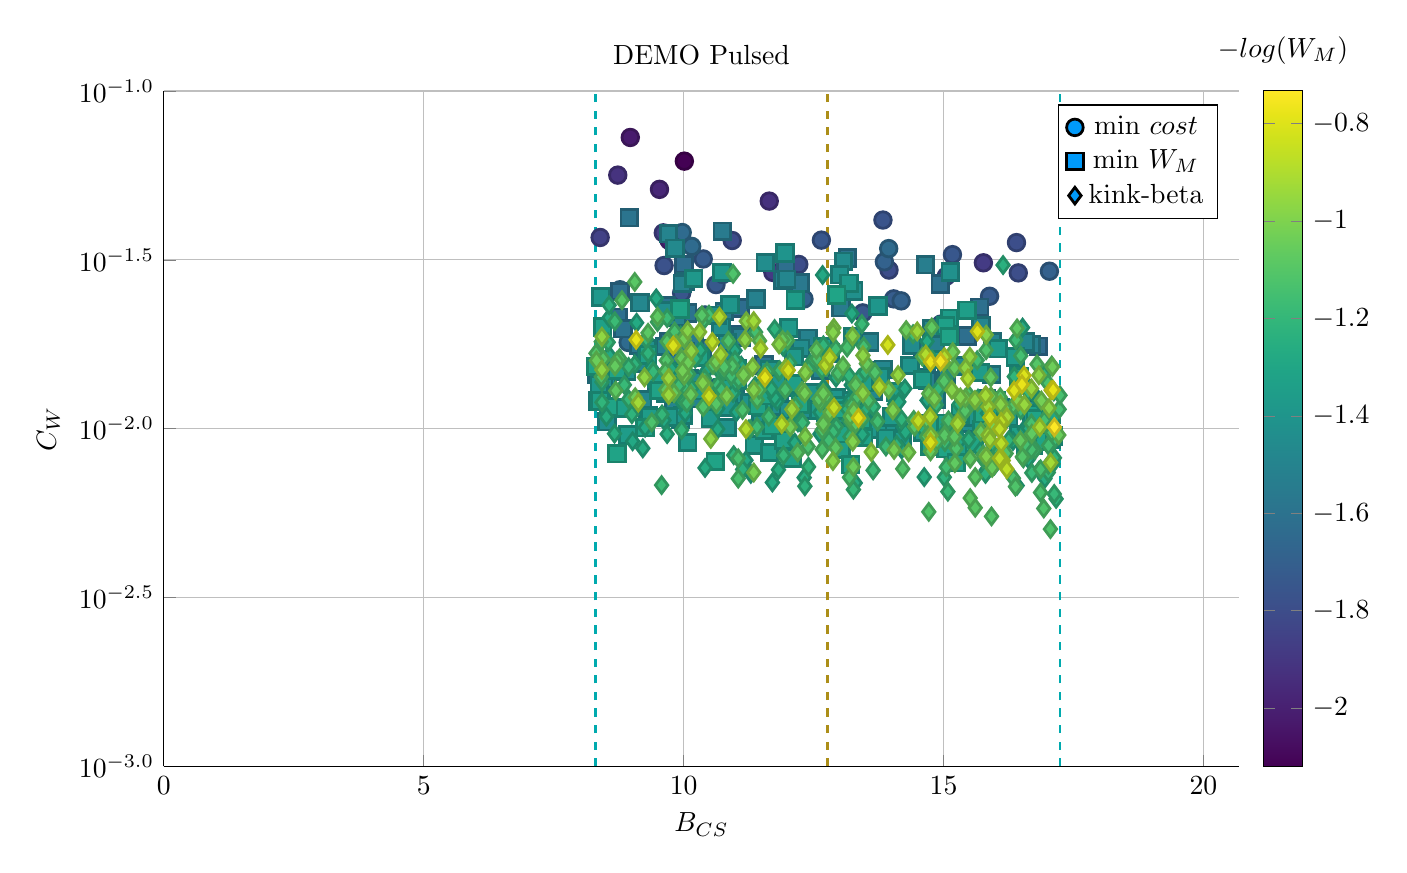
\begin{tikzpicture}[]
\begin{axis}[colorbar = {true}, height = {101.6mm}, ylabel = {${C}_{W}$}, title = {DEMO Pulsed}, xmin = {0.0}, xmax = {20.686629468551892}, ymax = {0.1}, ymode = {log}, xlabel = {${B}_{CS}$}, {unbounded coords=jump, scaled x ticks = false, xticklabel style={rotate = 0}, xmajorgrids = true, xtick = {0.0,5.0,10.0,15.0,20.0}, xticklabels = {0,5,10,15,20}, xtick align = inside, axis lines* = left, scaled y ticks = false, yticklabel style={rotate = 0}, log basis y=10, ymajorgrids = true, ytick = {0.001,0.0031622776601683794,0.01,0.03162277660168379,0.1}, yticklabels = {$10^{-3.0}$,$10^{-2.5}$,$10^{-2.0}$,$10^{-1.5}$,$10^{-1.0}$}, ytick align = inside, axis lines* = left,     xshift = 0.0mm,
    yshift = 0.0mm,
    axis background/.style={fill={rgb,1:red,1.00000000;green,1.00000000;blue,1.00000000}}
, colormap={plots}{rgb=(0.26700400,0.00487400,0.32941500), rgb=(0.27794100,0.05632400,0.38119100), rgb=(0.28291000,0.10539300,0.42690200), rgb=(0.28229000,0.14591200,0.46151000), rgb=(0.27619400,0.19007400,0.49300100), rgb=(0.26514500,0.23295600,0.51659900), rgb=(0.25042500,0.27429000,0.53310300), rgb=(0.23360300,0.31382800,0.54391400), rgb=(0.21813000,0.34743200,0.55003800), rgb=(0.20123900,0.38367000,0.55429400), rgb=(0.18555600,0.41857000,0.55675300), rgb=(0.17117600,0.45253000,0.55796500), rgb=(0.15772900,0.48593200,0.55801300), rgb=(0.14618000,0.51541300,0.55682300), rgb=(0.13374300,0.54853500,0.55354100), rgb=(0.12346300,0.58168700,0.54744500), rgb=(0.11948300,0.61481700,0.53769200), rgb=(0.12632600,0.64410700,0.52531100), rgb=(0.15014800,0.67663100,0.50658900), rgb=(0.19109000,0.70836600,0.48228400), rgb=(0.24607000,0.73891000,0.45202400), rgb=(0.31192500,0.76782200,0.41558600), rgb=(0.37777900,0.79178100,0.37793900), rgb=(0.45867400,0.81636300,0.32972700), rgb=(0.54552400,0.83803900,0.27562600), rgb=(0.63690200,0.85654200,0.21662000), rgb=(0.73088900,0.87191600,0.15602900), rgb=(0.81457600,0.88339300,0.11034700), rgb=(0.90631100,0.89485500,0.09812500), rgb=(0.99324800,0.90615700,0.14393600)}, colorbar style={title=$-log( W_M )$}}, ymin = {0.001}, width = {152.4mm}]\addplot+[scatter, scatter src=explicit, only marks = {true}, color = {rgb,1:red,0.00000000;green,0.60560316;blue,0.97868012},
draw opacity=1,
line width=0,
solid,mark = *,
mark size = 3.0,
mark options = {
    color = {rgb,1:red,0.00000000;green,0.00000000;blue,0.00000000}, draw opacity = 1.0,
    fill = {rgb,1:red,0.00000000;green,0.60560316;blue,0.97868012}, fill opacity = 1,
    line width = 1,
    rotate = 0,
    solid
}] coordinates {
(10.014310061470209, 0.06197483174638786) [-2.119809409407475]
(8.974351824202143, 0.07282952610606806) [-2.022107373269494]
(9.720840649522977, 0.03609135913093006) [-1.9777667149411715]
(9.535747921961464, 0.051130362720294704) [-1.969913275543008]
(11.64719575750508, 0.047199699242522014) [-1.9276279243167613]
(8.733488072843636, 0.05634035623848662) [-1.9180907603558137]
(11.717151268119157, 0.0290156978870517) [-1.8866814459155106]
(15.76615725864231, 0.030992141550921816) [-1.8810042714594786]
(9.609717770109604, 0.03801538835634297) [-1.861231108978198]
(8.394527886005427, 0.03683114347875789) [-1.8558362580925096]
(15.053294230728687, 0.028291519575269056) [-1.811508198071671]
(10.934532396569558, 0.03607745072820276) [-1.8048956433290855]
(12.215380678409446, 0.030644555029908985) [-1.797922304180305]
(13.950900000393457, 0.02949537628440487) [-1.7974494679074275]
(16.437201647022366, 0.028933124859920306) [-1.7961193741663348]
(16.40261361811642, 0.03557653455378664) [-1.7922955251500743]
(9.624471357573801, 0.030417392770278703) [-1.7763653379983415]
(13.834221351663881, 0.04147970255534964) [-1.762574168304495]
(9.962006621581514, 0.025210912703269035) [-1.7524000959584443]
(12.65031002841598, 0.036173737778618126) [-1.7467043012053995]
(15.171180859324355, 0.032766263996239824) [-1.7445197156480476]
(13.447185867051214, 0.02202338694073385) [-1.7362913649987812]
(10.622905984575329, 0.026714074548194577) [-1.7340594740544224]
(9.687508349386887, 0.022713661122324157) [-1.7289223235866222]
(15.885358349462447, 0.02466928657304406) [-1.719614121069955]
(14.041145822343132, 0.024233508820652228) [-1.7167136137505041]
(10.377907964259716, 0.03181143352229567) [-1.7154437116459917]
(10.753780577931199, 0.028622291298276443) [-1.7060722509483957]
(17.03614113083419, 0.02926238447048653) [-1.6937830944780397]
(13.861622812084057, 0.03120868171359675) [-1.6889812321302553]
(14.184282250063832, 0.023905595143656186) [-1.686209077026567]
(12.315442430684204, 0.024204963735087338) [-1.6786883535604935]
(14.950434999553853, 0.020413682949498045) [-1.6734478593396724]
(10.4122328117203, 0.02171708878277083) [-1.650681965327452]
(8.776130848827346, 0.025789595420542006) [-1.6458495153344535]
(13.944616671700327, 0.034141771708853026) [-1.6412636709027566]
(9.972964073735131, 0.03809649700399676) [-1.6393314314904326]
(10.155668028711606, 0.0346599142742729) [-1.6390302509540549]
(8.93332912842768, 0.018002375584230325) [-1.6381696948341165]
};
\addlegendentry{min $cost$}
\addlegendentry{min $W_M$}
\addlegendentry{kink-beta}
\addplot+[scatter, scatter src=explicit, only marks = {true}, color = {rgb,1:red,0.00000000;green,0.60560316;blue,0.97868012},
draw opacity=1,
line width=0,
solid,mark = square*,
mark size = 3.0,
mark options = {
    color = {rgb,1:red,0.00000000;green,0.00000000;blue,0.00000000}, draw opacity = 1.0,
    fill = {rgb,1:red,0.00000000;green,0.60560316;blue,0.97868012}, fill opacity = 1,
    line width = 1,
    rotate = 0,
    solid
}] coordinates {
(16.82228492576424, 0.017540808339758972) [-1.6348798048481208]
(11.091923619988552, 0.022785258097976623) [-1.6277277898588538]
(10.00476818341642, 0.030625514244526048) [-1.627684330571819]
(8.777176250808912, 0.025489957683783454) [-1.6248467182009472]
(10.991846079958428, 0.0189830433690413) [-1.62256122166559]
(15.458683088869776, 0.018838350678554387) [-1.6197529434592726]
(11.964070298839442, 0.030553347689269015) [-1.619473374550493]
(8.73450389120548, 0.0213568595963161) [-1.6190205769362032]
(14.592694375647465, 0.017173711360022336) [-1.617478678707941]
(15.693294727899161, 0.022891816741403965) [-1.6135161817566324]
(14.936949374526826, 0.026834336105762403) [-1.6079101518459553]
(8.83184401567771, 0.01976733422078956) [-1.6005797137016178]
(9.72150547040655, 0.01811055755791537) [-1.5991182248913247]
(10.078203743630864, 0.02202289176749285) [-1.595836360479248]
(8.954209756242996, 0.042161103004000076) [-1.589397412964098]
(9.673607099925281, 0.0231728109038665) [-1.589205111302375]
(11.543935756448146, 0.015450272567257462) [-1.5875377953010883]
(13.151617966814817, 0.0319953061173649) [-1.5845809864087244]
(9.781030534247606, 0.016164039710660088) [-1.5775674018565111]
(9.303102469493684, 0.016693759971981265) [-1.5713155071601692]
(10.359872502096119, 0.01726409176752251) [-1.5652457853616617]
(12.237632180874417, 0.02698353416604086) [-1.5643952661253622]
(9.144801617136775, 0.01769761001811183) [-1.5595601870169422]
(13.029635600163276, 0.02281153437267921) [-1.552568848396255]
(10.7422001331706, 0.038423068705951594) [-1.5520441226990631]
(10.780757247562724, 0.022224095489930037) [-1.544925041354305]
(10.200715682654506, 0.01841847429182733) [-1.5430023738862098]
(15.017329028039686, 0.019477644457703495) [-1.5396243114452017]
(8.334002624663501, 0.01449908817629988) [-1.538692217528126]
(10.555701885198872, 0.013092644307368572) [-1.5373740781698282]
(14.65414605441725, 0.030574977212997605) [-1.5350312948909135]
(14.660222353908768, 0.014205258889817484) [-1.5317433014682034]
(11.106568774256633, 0.018689708848548738) [-1.5311850486265117]
(14.689056206740792, 0.01387590038164943) [-1.5287451237254033]
(9.473959265162193, 0.013905952265261586) [-1.526526816139614]
(10.035372496295135, 0.027241135712482305) [-1.519178921439465]
(10.039027121575653, 0.016910779414334946) [-1.517891032933806]
(11.39227618908412, 0.024191852864153648) [-1.5130165343032327]
(16.679321236285688, 0.01773125993862434) [-1.5126055054907948]
(11.906042879430306, 0.027530426264504002) [-1.5122759735909235]
(13.642157714321597, 0.014899481481132758) [-1.5121531835443067]
(14.850116736119897, 0.01778122202031051) [-1.5121518481580156]
(12.392450828732116, 0.01852162588841651) [-1.509963665969106]
(11.613487062213123, 0.013259386458548635) [-1.5098191352881933]
(13.579000388347866, 0.018078145365757758) [-1.5094600237705913]
(9.867201865947047, 0.02134336001409843) [-1.5091677016781566]
(9.643385161260726, 0.017507453096671365) [-1.505813383704145]
(9.97586799244543, 0.026909424888676328) [-1.5035180904231982]
(15.94212072748298, 0.018116695499993292) [-1.4998070828001184]
(10.309179324950696, 0.01226652304303364) [-1.4993412700061268]
(12.638042249859588, 0.014898889997617197) [-1.4970388348465338]
(15.055675671525783, 0.014279317114283529) [-1.4968151314329754]
(9.710222870228767, 0.03778412752723575) [-1.4959262215207656]
(9.813107231605422, 0.012007443130458324) [-1.495878750102406]
(9.685925965003944, 0.014131383104205364) [-1.4911760171512294]
(11.714098265194735, 0.013847785437885679) [-1.4909012021072667]
(10.994639674638705, 0.013113327535403696) [-1.4904727997922445]
(15.819989093254375, 0.012253217681920671) [-1.4902975254497872]
(15.716610680795545, 0.020179920200301855) [-1.4899596862430686]
(15.924465247564154, 0.014465480638895564) [-1.484315053758591]
(8.416214966248592, 0.012974868808400592) [-1.4832272441818983]
(11.981607928881237, 0.02767164571202513) [-1.481908947186888]
(11.711067257135763, 0.012700241486954703) [-1.481610811848838]
(16.57758432667383, 0.018066556725317685) [-1.4808315890609627]
(9.214130290028436, 0.012152582495637852) [-1.4803924190961808]
(9.16252648162826, 0.023591043628319753) [-1.4777813991456452]
(13.841485576616298, 0.014987126189756067) [-1.476226145125234]
(14.86036210936636, 0.012179602718049342) [-1.476103765156545]
(14.771702357628312, 0.0198044997246676) [-1.4759532635696884]
(11.751019990155784, 0.011854698849849837) [-1.4744693843941874]
(9.214130290028436, 0.015665176708494814) [-1.4721189566530006]
(13.644386027863185, 0.012892988065699775) [-1.4694765884704042]
(12.673551051198132, 0.011723605612914264) [-1.4684762544315009]
(16.7437460203336, 0.01146148363735155) [-1.4673712598422484]
(10.114476569413018, 0.01403086783418577) [-1.4665127712450712]
(9.836829838606402, 0.03422172209265897) [-1.466465342676487]
(15.478205114940627, 0.011814056076879775) [-1.4656409913573911]
(10.852786830516008, 0.01666169164744686) [-1.4607639902508311]
(12.451557765219139, 0.011797068547740396) [-1.454804800167485]
(14.385054216404878, 0.017714850999176746) [-1.454016548396377]
(12.250517419581046, 0.01730924236440855) [-1.449126660054787]
(15.399238782030915, 0.015350811156516968) [-1.4450317564339483]
(15.323964495196108, 0.010700521525178483) [-1.4442476160174416]
(10.840350242413816, 0.017999193081243068) [-1.4428695943470562]
(13.07657469813823, 0.03129913412451443) [-1.4416527786165851]
(11.571153759168391, 0.030992801350489627) [-1.4412978501823663]
(10.159175807081688, 0.013876797144792313) [-1.4410674847520173]
(14.65870048492913, 0.0103371343106061) [-1.4407593364531412]
(9.64911680597678, 0.022291694526716137) [-1.4382523340904476]
(11.824660750219888, 0.011033535668865918) [-1.4374618391296154]
(16.090603216081107, 0.011578760205733224) [-1.437309497392895]
(8.526794202732354, 0.014225493350487712) [-1.437004502630189]
(11.836002040544534, 0.011662685993065088) [-1.4369516286418977]
(15.4684670810238, 0.010363517857158673) [-1.4359296968945898]
(11.551257449345478, 0.012593943496598788) [-1.4348111698815942]
(8.523380131000312, 0.010486068251726523) [-1.4347403934029699]
(12.329900028804074, 0.011351647420548932) [-1.432162507533083]
(13.236600826453692, 0.010703895251080882) [-1.4298959659652046]
(16.83282359352303, 0.010279170294604838) [-1.429141349371285]
(13.269307990860742, 0.025557043779995653) [-1.4288294492620477]
(10.717109038917776, 0.019981046165081038) [-1.4275892047251812]
(8.463326863230373, 0.014011150106021747) [-1.42664672926539]
(9.292495803166666, 0.017276630179413652) [-1.4239039330716527]
(12.01294221545527, 0.01135063897630595) [-1.4237047673472223]
(10.642574031409726, 0.021651736693319764) [-1.4220880228019461]
(15.130371291452986, 0.029124606257697153) [-1.4214589216983458]
(13.449121379363364, 0.010524080735331771) [-1.4192750546166355]
(10.598536227766495, 0.012152497168515361) [-1.4188846212567885]
(9.94286005160173, 0.010654264771940928) [-1.418142111238707]
(8.354283940274188, 0.012093014306414056) [-1.4175771687309422]
(11.490654672775422, 0.010307835186267926) [-1.4166515403180218]
(13.927755889931667, 0.009802839106844477) [-1.4151591623618127]
(12.896498202515414, 0.012089411129630757) [-1.415086999740124]
(12.813665090982388, 0.016771907819218872) [-1.4150518254702726]
(8.905845640255238, 0.01479570625667246) [-1.412750376425469]
(13.001742838316293, 0.02858609969916251) [-1.4118418857799215]
(14.802174067631956, 0.009976658176736495) [-1.411745253778192]
(11.208912070421409, 0.011899859669740264) [-1.4101129990450592]
(12.913000276070724, 0.010975696046095008) [-1.4098064292280077]
(10.84161307277213, 0.010078193568331789) [-1.4071217370506766]
(10.952245284131447, 0.012567870805096065) [-1.4069653518342513]
(15.465550241086678, 0.010809590548122633) [-1.4053188021751997]
(11.888760566686239, 0.013228123351848638) [-1.4040831795581317]
(9.656977955682123, 0.012756284815624411) [-1.403783408224447]
(12.357969070297273, 0.011849909135487101) [-1.4034059706684434]
(14.354705949019486, 0.015391572104901911) [-1.4031334212883295]
(15.759091197715701, 0.011370525417095621) [-1.4027031557706915]
(15.93492167661274, 0.010883116023126084) [-1.4023409214316394]
(11.950351989604266, 0.03314304390232683) [-1.4018234466267534]
(9.31395933016945, 0.010943279854872806) [-1.4001967788421508]
(12.501198744996175, 0.012776602146795163) [-1.3983213447403338]
(16.691702745627914, 0.011065372696240975) [-1.3946316971345938]
(12.793680134727829, 0.009697674748088487) [-1.393981306323598]
(12.945145532203291, 0.012316212001497684) [-1.3939743444895971]
(10.895241072523511, 0.023293627402023516) [-1.3938659098694006]
(10.624418674781085, 0.012799262525216688) [-1.3934317035795]
(13.736998867652822, 0.02306752096780418) [-1.3919378361313393]
(10.86446674023058, 0.011575943181240602) [-1.3913501343623875]
(9.989604552735361, 0.010938935413839007) [-1.3899986150261634]
(11.65036209258509, 0.014916276865219583) [-1.3888953225499234]
(16.253794354777128, 0.010811642128190005) [-1.3883849558567678]
(13.237511348589962, 0.012086573842968483) [-1.3880683151937296]
(13.3098445206835, 0.00974951527611275) [-1.3879257169733152]
(13.250391582535599, 0.01875474559032549) [-1.387200255154835]
(10.737511566041665, 0.028992717747430105) [-1.3869139374162498]
(13.77662330230216, 0.014275341697562267) [-1.385982080919773]
(15.808216920395289, 0.009658736241223327) [-1.385951966541943]
(13.731078012406766, 0.009979205376142167) [-1.384341496966052]
(14.597629824496682, 0.009781750047901397) [-1.3836628266676982]
(10.193517952021443, 0.027837899406166513) [-1.383138617240496]
(11.85882016006122, 0.013692957043690078) [-1.3831333668949872]
(15.990533435344123, 0.012055028195149642) [-1.3823755173012382]
(8.403151177328072, 0.02457168150365556) [-1.381386436684111]
(8.38045546510813, 0.013467436970042478) [-1.381013926041926]
(12.120810510968868, 0.01632900764605371) [-1.3807582017142732]
(10.203415923531363, 0.016233342907168043) [-1.3795912650626003]
(12.022820996636117, 0.019856726760879642) [-1.3784744825946547]
(14.941654987190931, 0.009937020814786353) [-1.3784050115817357]
(10.30431640058217, 0.012947457233964572) [-1.3727350903904059]
(13.179314023604123, 0.02692798924274793) [-1.3726382795387042]
(11.360939883051167, 0.00894061047284123) [-1.3726183217257064]
(9.712824116971364, 0.01083618948017438) [-1.370506635821487]
(13.999353699862713, 0.010820381028973857) [-1.3702834841058706]
(11.029519708444795, 0.01507474130083674) [-1.3699905172740252]
(14.790388677939154, 0.016024901755414496) [-1.3694510931398833]
(14.2011289491935, 0.009286958803152093) [-1.3690194932725448]
(16.05186059099198, 0.01725165686414962) [-1.3685993689556193]
(10.079551280694128, 0.009100422809121853) [-1.3680782620249432]
(13.891099279827657, 0.009358898748733285) [-1.3659937757563743]
(10.51469839684549, 0.010741593794976297) [-1.3655266043175585]
(16.97679926285361, 0.00935804014953258) [-1.365489135635999]
(16.382025622806193, 0.01631624677926724) [-1.365314944668722]
(12.601871821561915, 0.011316654652064283) [-1.3620488306806053]
(9.342717740515683, 0.010811158792461435) [-1.3600883836878876]
(15.699013106793902, 0.014663988794896813) [-1.3569999482959285]
(17.08124053314885, 0.009327975573933072) [-1.3565369493574833]
(8.929819918270683, 0.009591330831744169) [-1.3564434514013937]
(17.107810871536294, 0.009510520762087537) [-1.355670949654743]
(15.272532347809275, 0.008600603815848054) [-1.3550689180362785]
(15.113272758939148, 0.0212306523206366) [-1.3545717493575382]
(12.758115395547385, 0.011027495783414606) [-1.3536406793714741]
(12.146510141523258, 0.02403578580290836) [-1.3522480304376618]
(9.802895887224908, 0.01277987363566607) [-1.351683168790268]
(12.731812711004267, 0.011181317227288103) [-1.3509416538039447]
(14.597629824496682, 0.013988110662625983) [-1.350917699634303]
(12.937418062164188, 0.011706003302806382) [-1.3498675794038522]
(12.680634700802198, 0.01744787935363008) [-1.3480954361555229]
(16.547895069902516, 0.009513333911267541) [-1.3474307155472665]
(11.653216567545261, 0.008506399274340092) [-1.345835600508895]
(15.44880839508013, 0.022402494346273383) [-1.3441619287129023]
(11.525312140201327, 0.011568935524735228) [-1.343173024895477]
(11.552250427675727, 0.009888039453025594) [-1.3431102335422052]
(13.467268933575436, 0.013676025720795522) [-1.3418959513921676]
(15.323265928492141, 0.011055478792069253) [-1.3416390955818198]
(12.121641590617898, 0.013562184857025608) [-1.3412225668983788]
(11.024065356801717, 0.013928329166195007) [-1.3411223781363122]
(16.734724817567656, 0.008957609956171385) [-1.3409980727589041]
(16.769045540215842, 0.011061155580644737) [-1.3407774046291352]
(9.473959265162193, 0.014142372730384274) [-1.340736718067575]
(8.74505555084563, 0.014931289500105476) [-1.340172101894623]
(13.027598279499255, 0.008673821452175847) [-1.339371225527388]
(14.069726621490684, 0.012851757813003692) [-1.3355889626958743]
(16.45157670371507, 0.009585198585080813) [-1.3353537500446666]
(8.828372531773972, 0.011502571386254939) [-1.3352936153265889]
(15.043191855376238, 0.020177908654106694) [-1.3347167954999664]
(15.87555423129121, 0.010934192827515073) [-1.3333464153994234]
(14.74050555979749, 0.010187040046408826) [-1.3319467069356516]
(8.394635001603197, 0.012093243108414115) [-1.3317606682979195]
(15.737459460817936, 0.0099544891977854) [-1.330878268232421]
(16.577004376563345, 0.00892167491417854) [-1.329838199225075]
(8.442119987401155, 0.020024514359414238) [-1.3275817805394716]
(15.03780769292473, 0.010377685225384297) [-1.3271981479523673]
(11.923687420170552, 0.00923521460571462) [-1.3257753666633474]
(9.311244990438865, 0.016536435428404248) [-1.324805801675252]
(12.08205721926947, 0.008177838551829547) [-1.3236480395933032]
(10.75205842676705, 0.01320289357034274) [-1.3223872875360454]
(13.461717625918478, 0.009416665871049234) [-1.320790714548859]
(9.519960674752117, 0.012966997564871513) [-1.3198610091294973]
(8.715815013641683, 0.014941915896507264) [-1.3173999901029887]
(9.815532890733682, 0.014705731648914599) [-1.3172398911361078]
(15.109422453252336, 0.018745840734049092) [-1.3155841266914403]
(14.740296253242736, 0.008883845818604448) [-1.3144429555765318]
(10.31653236444549, 0.016334708642476756) [-1.3140984246311314]
(10.60954534582113, 0.007999169369094802) [-1.3136141988883636]
(13.432319600929263, 0.010593671042148305) [-1.3130409307938926]
(11.42823386655995, 0.011696426000066894) [-1.312883593567563]
(8.719380611168567, 0.008437215022084032) [-1.3113636666391015]
(11.696923395666094, 0.010210442889078589) [-1.3110543205827916]
(8.560854879579562, 0.01161135507437133) [-1.3101666476591896]
(16.764368284085073, 0.010715857251244127) [-1.3094281744638252]
(15.192999611497397, 0.007935513211517508) [-1.3092819198295769]
(8.315725665672304, 0.01527961135499392) [-1.3091789421820008]
(15.043366759433116, 0.008718673720708605) [-1.308657609117127]
(16.021238035205084, 0.012115862676003172) [-1.30815684782275]
(11.593073557294613, 0.012528702800938256) [-1.3073192126014976]
(15.192999611497397, 0.009466859805614364) [-1.306104667504652]
(12.945145532203291, 0.024862203238592617) [-1.3061029424340123]
(9.927382980222017, 0.022588731344076834) [-1.3059932173472433]
(9.256949266351661, 0.010067194372351543) [-1.3053424100316993]
(16.82199006964077, 0.009194414774426339) [-1.3048906180553326]
(16.45157670371507, 0.014224364223609164) [-1.3043596581137094]
(13.051048964875424, 0.00966642720928779) [-1.304157201921016]
(15.244913096432274, 0.007934056288357859) [-1.3040523349428945]
(12.245141259071001, 0.011830250137913223) [-1.3039439069452712]
(16.026769470614276, 0.008152912507864905) [-1.3022467953572583]
(13.051048964875424, 0.011323662495891916) [-1.3012176243848619]
(15.591542980066137, 0.009074217857747638) [-1.3011866801418175]
(17.068912884842916, 0.011011974496683653) [-1.3004916659282275]
(13.212953491584514, 0.007824745570931163) [-1.3001880033121107]
(15.749170807222828, 0.011078402389842862) [-1.2993649239636758]
};
\addlegendentry{min $cost$}
\addlegendentry{min $W_M$}
\addlegendentry{kink-beta}
\addplot+[scatter, scatter src=explicit, only marks = {true}, color = {rgb,1:red,0.00000000;green,0.60560316;blue,0.97868012},
draw opacity=1,
line width=0,
solid,mark = diamond*,
mark size = 3.0,
mark options = {
    color = {rgb,1:red,0.00000000;green,0.00000000;blue,0.00000000}, draw opacity = 1.0,
    fill = {rgb,1:red,0.00000000;green,0.60560316;blue,0.97868012}, fill opacity = 1,
    line width = 1,
    rotate = 0,
    solid
}] coordinates {
(14.682772921069034, 0.012133883145293747) [-1.2971735267311564]
(16.555137236197424, 0.008497507185750146) [-1.2963451470925318]
(13.179991464330723, 0.011968595839803002) [-1.2939289874566402]
(15.888696111510232, 0.008051203599652048) [-1.2928570974581939]
(16.651463466334494, 0.009198462479520332) [-1.2926592596370523]
(16.555137236197424, 0.009976448637174172) [-1.2918359622137705]
(11.015371517921224, 0.011200517330116096) [-1.2901565279273088]
(10.43448368514836, 0.014778677283745992) [-1.2885231243501492]
(12.62262254375668, 0.009645840422057206) [-1.2873870680148987]
(11.10781988195937, 0.015368153744705897) [-1.2867189599495152]
(16.82199006964077, 0.012200186404574626) [-1.2866608738447551]
(15.327000264646497, 0.009314200607444962) [-1.2862989627940875]
(11.293041040527157, 0.007351086075188858) [-1.2856479743658245]
(12.62262254375668, 0.011184811263709776) [-1.283461572944208]
(12.673551051198132, 0.028511756618296732) [-1.282628142229196]
(9.018740260054527, 0.0091809969411667) [-1.282318795548118]
(9.378254722237372, 0.015147418693115068) [-1.2809419797501462]
(16.67207354194001, 0.009441743395354373) [-1.2802239523296417]
(14.221898977802105, 0.010115067051441084) [-1.279661807174519]
(14.193898850417899, 0.008682653521467484) [-1.2793586996677089]
(16.335988065907316, 0.00919694313697991) [-1.279241431080542]
(11.199032883922865, 0.008062649665833432) [-1.2791738597664242]
(8.565625511562189, 0.016537125137685977) [-1.2777724695025643]
(9.473959265162193, 0.024311609583825906) [-1.2776560252665474]
(15.820537682670786, 0.007543708329813699) [-1.2776226586446298]
(13.223938971427943, 0.013472425466080754) [-1.2772080908839465]
(9.6224419440208, 0.010591022499429533) [-1.2768888641183538]
(9.259381405997736, 0.010068814155906535) [-1.2749252706301877]
(10.02950074316046, 0.011122028940902477) [-1.27405635520294]
(9.096410727756737, 0.020592443763116842) [-1.273999627133777]
(11.250274296159523, 0.009932693135460512) [-1.2739263340884897]
(16.651463466334494, 0.013177764718534145) [-1.273686836355838]
(13.236600826453692, 0.021930543698997433) [-1.272060671091855]
(10.988390518242154, 0.01703366147805158) [-1.2717552020206426]
(12.689774417510133, 0.013199694993892157) [-1.2715552113887816]
(14.682772921069034, 0.018137179053328113) [-1.2711256143593725]
(12.138235311074201, 0.009089213335736035) [-1.2706918059143955]
(16.51983071545539, 0.019922160606497104) [-1.270659241243097]
(13.440224729488612, 0.009612072783370788) [-1.2706266042708976]
(14.056438663449487, 0.011815687417752718) [-1.2699973230973551]
(16.632293213183402, 0.008127375094877596) [-1.2694883213650459]
(15.843105813982604, 0.011108460101523684) [-1.269469949244091]
(14.139022745673238, 0.01200413289507089) [-1.2693810054133523]
(8.565625511562189, 0.021322131632939743) [-1.2685038799823198]
(9.215460716271485, 0.008746022086925008) [-1.268011220133286]
(11.79925508433291, 0.012071261699451271) [-1.2676767161765092]
(9.767648689516832, 0.015027760071695463) [-1.2672360183442966]
(9.905927226247794, 0.012386782250268949) [-1.2670329245716005]
(10.65725161660864, 0.00997135774995843) [-1.266521603924258]
(10.055681915858392, 0.014743359804979298) [-1.265829536383991]
(12.138235311074201, 0.011015221663609409) [-1.2655850749955841]
(14.267102900143742, 0.009754591610171831) [-1.2651606387913807]
(16.568716501758974, 0.008391084675782472) [-1.2650267302153226]
(10.65725161660864, 0.011459660264397842) [-1.2643165163116283]
(14.25689481086506, 0.01314380020899071) [-1.2638630587832318]
(16.632293213183402, 0.0100188505842072) [-1.263682663264664]
(11.707584495779955, 0.006930908540990179) [-1.2635507051033026]
(10.412391370371594, 0.007655768190498255) [-1.2630930817893484]
(15.707955638238712, 0.008595102325139414) [-1.2620028969039807]
(15.941689167985352, 0.008993269936185943) [-1.2617711256664215]
(11.618449420251658, 0.013435175267701598) [-1.2607622270815175]
(11.906052951232901, 0.010399130132164968) [-1.2599969566754825]
(13.422765787398976, 0.011066872440514844) [-1.2580199333772297]
(12.931935336308614, 0.014164623239439114) [-1.257674742909116]
(16.4155019400067, 0.006784814729690784) [-1.256920205986828]
(8.514832197721942, 0.010847484174753686) [-1.2558826127376497]
(9.960307841751561, 0.012006910499828622) [-1.2545784323742915]
(11.751019990155784, 0.012367303307791636) [-1.2541769145790829]
(13.300908706718086, 0.006909773766752695) [-1.2538081670568602]
(16.949195577210475, 0.007118806510545466) [-1.2537331036632384]
(12.318542112721676, 0.007163920014099904) [-1.2523947287534352]
(9.960307841751561, 0.01409766195530951) [-1.252161894882265]
(14.628561786858135, 0.007191926525759095) [-1.2517841257242934]
(15.90674460516089, 0.010140660180167243) [-1.2510148685101052]
(12.87923916901645, 0.009947685467565285) [-1.2503817284236358]
(11.824591933033416, 0.00755783116205777) [-1.2500618007814928]
(10.31927503264005, 0.01705584468677382) [-1.249408930050928]
(15.977434181824485, 0.007782048369656626) [-1.248434923528094]
(9.683456615169344, 0.009638865392082259) [-1.246475793101881]
(8.671623187801623, 0.009668090359024908) [-1.2453083223674235]
(15.299311115315916, 0.01181801423349667) [-1.2430271033455136]
(10.952245284131447, 0.012765537294567253) [-1.2425009663963265]
(13.37865937666007, 0.014096920088512531) [-1.2420036959161107]
(11.040941770182885, 0.014638041989732616) [-1.2406291651922927]
(13.488578301097156, 0.011330221246013529) [-1.2404081246835275]
(14.628561786858135, 0.009882346466549934) [-1.2402721066912186]
(16.145232878087864, 0.030517882462548936) [-1.2399829928026451]
(9.943887569980818, 0.018855374361929193) [-1.2398403601837327]
(11.689159647203805, 0.013105067185166342) [-1.2382227382575577]
(8.567148568313412, 0.023206171452307512) [-1.2372685823332665]
(11.915585134033648, 0.01748239328622686) [-1.2369979991721363]
(12.198645212509877, 0.010436966421480154) [-1.2364971528125899]
(15.48431465614079, 0.00929031971105747) [-1.235918342000411]
(9.047649397424134, 0.01224311754662533) [-1.235332112263366]
(11.376707871371156, 0.013377000135851953) [-1.235230354209212]
(16.840748740961537, 0.00752176857171885) [-1.2348662947331168]
(11.136175174634447, 0.007577390318458053) [-1.2331237451825037]
(14.097655097755435, 0.008954934736687754) [-1.2314216648450123]
(15.807042377277515, 0.007348723496235854) [-1.2276908244938955]
(12.33207356829479, 0.00675688814735783) [-1.2234874983546444]
(10.222252038737434, 0.01611655322423877) [-1.2224132121245386]
(16.251358747135995, 0.009234491873309686) [-1.2212129344183997]
(12.723834447815875, 0.012691970303684906) [-1.221000044288545]
(9.004625505986517, 0.011032294768272291) [-1.2201668573985105]
(10.678976402706837, 0.014875616723151944) [-1.2200113852982524]
(13.05961095465478, 0.014755597501979523) [-1.2200110437170943]
(9.058040813922531, 0.015480160187022769) [-1.2199386530853975]
(11.751019990155784, 0.019725018407248666) [-1.2192027637421239]
(15.662199761760458, 0.01227428321856098) [-1.218844626416703]
(11.002753780917594, 0.013727476887235461) [-1.2187513907488479]
(15.014532020154196, 0.007184219051293641) [-1.2182120816961266]
(13.148749979709805, 0.011425165896800414) [-1.2178523450390264]
(9.316969297353253, 0.01671459075301228) [-1.217564445140848]
(10.154270603961049, 0.01316079396243774) [-1.2148287908302686]
(14.19279870188835, 0.010653867811546877) [-1.2144650329368094]
(17.165092473837838, 0.006198307301760009) [-1.2142295699793069]
(15.014532020154196, 0.009725241928162248) [-1.2114971471794018]
(10.964602796324286, 0.00834877000609595) [-1.2110590840755884]
(12.25459113238908, 0.010394495894857034) [-1.210956786812969]
(13.649393629962841, 0.01160689504064373) [-1.210625479626572]
(12.40274647042282, 0.007709496307162327) [-1.210548450407708]
(8.42941267292461, 0.01196700634860152) [-1.2101072964851303]
(16.360665913232772, 0.014267222031421351) [-1.2097043828037173]
(12.688686022519612, 0.017649120721508472) [-1.2090548152300868]
(17.101933862003563, 0.00786922573538261) [-1.2089432452477198]
(13.212953491584514, 0.018050177035811292) [-1.2088567702310062]
(8.42941267292461, 0.01374396978202603) [-1.208355792529063]
(15.807042377277515, 0.012119563498851512) [-1.2079597098695036]
(11.826932290539112, 0.01476620759208673) [-1.2069143247822283]
(16.937250320827843, 0.014425121215984256) [-1.2060355587049236]
(16.56929514507332, 0.008818373193963157) [-1.2051439881244612]
(13.181524156722897, 0.014347196234709005) [-1.2048202874468241]
(14.89986738586979, 0.013090961135950088) [-1.20412102013171]
(17.131922906542755, 0.008195788944222735) [-1.2006084749599055]
(9.584782689444218, 0.011017845567179161) [-1.1997509076464346]
(13.490860552242111, 0.01471498897475931) [-1.1989561148134826]
(13.176473234117513, 0.010576750792174504) [-1.1977552093777106]
(10.988245035999599, 0.015955953274896677) [-1.1973464324024234]
(15.038409502255757, 0.014024797653122234) [-1.1952843257986516]
(9.961762717388044, 0.009913142251828634) [-1.194608172565493]
(8.942050925672243, 0.012231614304186931) [-1.1943983553124515]
(17.120985015074893, 0.012895825589119291) [-1.1943709063726027]
(11.920999462954518, 0.008341248647504823) [-1.193465520169887]
(17.014436731421398, 0.007422215660710276) [-1.1934529196767811]
(8.548963250971841, 0.018029259293378272) [-1.1932608414538086]
(9.416726619046099, 0.01475503745943627) [-1.1930245850534404]
(12.4394525554187, 0.01559839957452813) [-1.19275308105931]
(13.265902368751764, 0.006601321305241876) [-1.1925650410586528]
(16.6299411017185, 0.012849471675853265) [-1.1916847830033912]
(17.129202501787184, 0.006406786662781295) [-1.1906829642457115]
(8.942050925672243, 0.015231829402577652) [-1.1905171502567853]
(9.27906715150467, 0.018424630927819426) [-1.1868792227109848]
(10.021428108030735, 0.012087057868798792) [-1.1860893620286155]
(14.77757376918867, 0.016048418150957987) [-1.1858875370196502]
(10.454025691365954, 0.011972397837837176) [-1.1854558952607928]
(8.86037108397972, 0.013483711604703155) [-1.1848213366225184]
(14.860405552114257, 0.011761816070313931) [-1.1847475832442582]
(16.697734081097174, 0.007399398212169979) [-1.1837916630431773]
(12.287202704452202, 0.010413257435217902) [-1.1834175022102877]
(13.199631705820181, 0.009470444499328991) [-1.1831305353511883]
(12.04002156741698, 0.015647472969860403) [-1.1828511911535706]
(13.429268295632518, 0.020407456319850734) [-1.181840770808167]
(15.083042498987238, 0.006510208938595967) [-1.1814651012301538]
(12.93585934283502, 0.010147346100150811) [-1.1809344434678004]
(15.08903520717264, 0.010306295906351105) [-1.1788261142099545]
(12.874280008939282, 0.00975845363999315) [-1.1783873972417303]
(9.683456615169344, 0.021255557406142055) [-1.1773891261145735]
(13.645133488301468, 0.007530050850229014) [-1.1772489110999693]
(13.89170225379231, 0.008856286376022381) [-1.1771937197283155]
(8.67737182027737, 0.02079595788529988) [-1.1768483795316644]
(10.771643002371896, 0.01477464262853022) [-1.1754670828809672]
(10.657856383500425, 0.013447350775475101) [-1.1748259721272571]
(16.06471023259536, 0.008533818365309384) [-1.1743579362801864]
(17.1316836490387, 0.00926629982316415) [-1.1731424023398116]
(15.026041337358697, 0.009127162071787865) [-1.1728411497954707]
(9.576609781620636, 0.006808109484569134) [-1.172547785671985]
(11.279560489781714, 0.009974514104150454) [-1.171293732602548]
(11.847882069406987, 0.014894587057756483) [-1.1706435645347975]
(12.662794223849232, 0.014934801738779929) [-1.1704804143126533]
(16.3897848180077, 0.018312728464608994) [-1.1694340492000508]
(10.730031930410188, 0.013038425730797958) [-1.1664836698360914]
(16.484580953127526, 0.011350876468389677) [-1.166021933665907]
(10.407320998161198, 0.014066615859663486) [-1.1653547583030963]
(11.639069714872814, 0.01085952514652926) [-1.1637013339225117]
(10.006343137186239, 0.013377410828925157) [-1.1629231949973953]
(11.059345377913772, 0.013971916288186385) [-1.1625677338545028]
(12.40274647042282, 0.01498663044146402) [-1.1615160270969884]
(10.06408250853542, 0.011904820041118874) [-1.1613847421954753]
(9.902431073117565, 0.013362365525672213) [-1.161380763910868]
(14.413146086048558, 0.019049310191542535) [-1.1612715538980343]
(11.410705501319088, 0.010122141818818486) [-1.1608808882180581]
(16.090315471306553, 0.011629604231527799) [-1.1602959592128257]
(16.535372216388026, 0.008169777889897055) [-1.1601187846950554]
(16.106899256187383, 0.00834966465898116) [-1.1597072302883453]
(10.09639230576176, 0.014522157751088465) [-1.1596295654776811]
(10.914467071854592, 0.014324434384547807) [-1.1584930595938716]
(15.760042238713773, 0.008145962416336265) [-1.1583013384515075]
(16.758572280032737, 0.008646050418225202) [-1.1578217536561153]
(17.018646604266053, 0.007816314398845932) [-1.1564044749404534]
(12.796253779221516, 0.009241849076330648) [-1.1562110876559482]
(15.052414924338043, 0.007695271029389756) [-1.1558406723410226]
(15.647072980506872, 0.015939165384127457) [-1.1551976368183803]
(13.731078012406766, 0.010505037613581628) [-1.1547723960660046]
(12.92675278881294, 0.01720072822154318) [-1.1547042721803664]
(17.018646604266053, 0.008918107308299703) [-1.1544971334332936]
(16.253794354777128, 0.011156083675037292) [-1.1514583143146417]
(10.39603038372212, 0.021035989307587558) [-1.150606587165903]
(13.463766396551701, 0.017520815218592205) [-1.1497568820513546]
(11.384733765960362, 0.019315926185319167) [-1.1488471764736738]
(16.484580953127526, 0.016442878704583205) [-1.14854127278881]
(11.604112098987112, 0.0147653907680726) [-1.1481443824350337]
(9.497296911957019, 0.02069244645197561) [-1.1475056240535222]
(10.488224449472721, 0.021750535713550727) [-1.147314943378139]
(17.223162892419708, 0.011413531346774588) [-1.1452162507505037]
(12.150894786402327, 0.011657490769208391) [-1.1440985305669964]
(16.68930628775202, 0.008671087589979474) [-1.143892607737901]
(16.569886893433157, 0.008990361186615302) [-1.1425154271844815]
(17.23885789045991, 0.012558201977665608) [-1.1419282223298928]
(16.936340179186345, 0.010576229210216307) [-1.1414111342865825]
(14.737732430469173, 0.010807673225691976) [-1.1409606377195203]
(16.68930628775202, 0.010350872866134037) [-1.140632380055554]
(13.442192340718403, 0.010685556097930418) [-1.1405059694207205]
(16.212323704366778, 0.010680444710790922) [-1.1402761489506106]
(11.549625061051866, 0.01443507208815689) [-1.1390460916159142]
(16.86604828682311, 0.007579718089160525) [-1.1390342976608838]
(17.08124053314885, 0.009743368571375198) [-1.1383859727853913]
(15.465550241086678, 0.011556690979889052) [-1.1378233474839952]
(13.14480493296275, 0.01739508549026366) [-1.1377132966757475]
(13.247068833500391, 0.011726874929476301) [-1.1376503199229564]
(11.050777266016288, 0.007116540390245059) [-1.1370921105287648]
(17.00860271346254, 0.013630883580602493) [-1.136359546149739]
(12.74928812237468, 0.01526251681202216) [-1.1362968805162]
(9.828339372234877, 0.019391120833403556) [-1.1358988321292471]
(16.412079199162257, 0.011860427509089479) [-1.1358539207185072]
(11.050777266016288, 0.008170611753766615) [-1.1356493088623822]
(13.190058867236672, 0.007176648981252689) [-1.1354932328782563]
(16.343118613330425, 0.007134995489417047) [-1.1335001124055868]
(11.133919631731134, 0.011362840629455528) [-1.1323762690185122]
(12.973701334746814, 0.014605309967466338) [-1.1314565774222176]
(11.954226224374837, 0.013041177771875015) [-1.1310401855629826]
(16.86506841916708, 0.006470994712702174) [-1.130758874865596]
(13.342005434244879, 0.01241454353087534) [-1.1307392487451149]
(16.12398815332631, 0.011706749993287805) [-1.129690412643984]
(15.094274129902931, 0.01058602765458819) [-1.1289684185709847]
(12.56748354328549, 0.016110870179123358) [-1.128250192514324]
(13.554151997056962, 0.012109336313631335) [-1.1252475037678356]
(12.394305575398981, 0.008853551975990904) [-1.1245713568718563]
(12.666314398171494, 0.008673362533302236) [-1.1245104109679405]
(9.38696353728333, 0.010444270942938963) [-1.1242443075431308]
(12.666314398171494, 0.009907337069737673) [-1.1228938533825863]
(8.76764666380086, 0.01617284927660436) [-1.1226570193988834]
(14.427153110649943, 0.010615516830489545) [-1.1219052279962924]
(10.952245284131447, 0.028747991383312018) [-1.1209037456306452]
(15.478205114940627, 0.012621272074607764) [-1.1208704370485616]
(8.416214966248592, 0.014241574824224812) [-1.1207611585447455]
(10.861478291017514, 0.018202292531005245) [-1.1203998091578635]
(10.565503795542257, 0.015435434654215487) [-1.1196814354947495]
(11.416396882862225, 0.012169534423588058) [-1.117569159173303]
(17.056046623244733, 0.0050427739927004075) [-1.1174068253287153]
(16.382905849179593, 0.006738702814170826) [-1.1173159767010323]
(16.927370682421678, 0.005804967663435989) [-1.1167239479963635]
(15.819310539767171, 0.01708642425533479) [-1.1164863253635564]
(10.935292177538425, 0.015330930676524145) [-1.115952177835906]
(15.239908563209354, 0.008749260299038544) [-1.1155484203276729]
(10.779261519279597, 0.015236234381945615) [-1.1150664792325955]
(9.666784021208144, 0.01592115312572862) [-1.1149932168726697]
(14.715771391147522, 0.005673676576267031) [-1.1142370448232701]
(13.680348432326898, 0.014668129539502894) [-1.1135938253905195]
(10.376299721045067, 0.011593058914657943) [-1.1130822843587194]
(8.416214966248592, 0.018098045276528054) [-1.1129520921882257]
(16.203212144020178, 0.00844667203200266) [-1.1124547143505663]
(8.3150929357084, 0.016721953817190965) [-1.1117755817247388]
(14.214820563676106, 0.007606086700097335) [-1.111280366817552]
(17.08124053314885, 0.015386499810507239) [-1.1101740400684632]
(14.874445961744078, 0.009178873934432705) [-1.1096152505342232]
(14.672482884458876, 0.00948558206580523) [-1.1091336694254372]
(15.922543129962769, 0.00549921046195563) [-1.1089472925298762]
(16.203212144020178, 0.010705864396776125) [-1.1083325350959032]
(15.5516399592509, 0.0120664731399153) [-1.1057691769416944]
(16.343118613330425, 0.01170188649136221) [-1.1052306881057743]
(9.648292020157323, 0.014780625174291278) [-1.1048342524266368]
(16.51628138673719, 0.00825332130192428) [-1.1040791363201474]
(9.681715451502004, 0.018112214499183755) [-1.10372942218946]
(15.414896999567594, 0.011298605446639833) [-1.103582476347948]
(15.009780791796173, 0.013827700265786854) [-1.1030780605127657]
(8.814332075489222, 0.024010256521613826) [-1.101931522650141]
(16.797173981743242, 0.015522113628368707) [-1.101867046977712]
(17.056046623244733, 0.00795138947787912) [-1.1003667806450579]
(10.352335102686904, 0.02165989163141366) [-1.0990677594380822]
(11.451280856994098, 0.013037664993115445) [-1.0985681498236441]
(8.452615406027144, 0.016081592594581397) [-1.09689970293996]
(16.090603216081107, 0.012393747498706212) [-1.096821122554822]
(12.734897998052263, 0.012434985279067572) [-1.0964121374005271]
(10.628802191532834, 0.01183751115186516) [-1.0959153745200985]
(8.719715276295174, 0.015872207284849116) [-1.0951138603994395]
(12.625983424173063, 0.01193697612442737) [-1.0935630581131108]
(14.441565116440211, 0.010142382786196016) [-1.0930015853658588]
(11.999367064518468, 0.01826314367748472) [-1.0926807345542335]
(13.229170763420015, 0.01049669131167502) [-1.092358598815151]
(15.608937873185686, 0.0058331827187052395) [-1.0903108179825227]
(12.193541408467336, 0.00850518416165101) [-1.0903092411067585]
(15.019675662549972, 0.009561398406421407) [-1.0901290311849905]
(9.060221474382915, 0.027205946824018463) [-1.0891338311139125]
(15.764959446173226, 0.008379371285638391) [-1.0890689103299427]
(15.608937873185686, 0.007192120489657057) [-1.0872838223167207]
(13.3098445206835, 0.010341548832271355) [-1.0871255562405924]
(14.59138120111165, 0.016346655642766064) [-1.0849442496417345]
(9.315924162741839, 0.019226877194134302) [-1.0838020887753101]
(12.601871821561915, 0.012250091200159203) [-1.082628205245438]
(12.924031262737543, 0.008783854738357962) [-1.0805808343660834]
(15.653030555639692, 0.012016404540784148) [-1.080271054774451]
(15.512646895146803, 0.006231165693590567) [-1.0801595841738052]
(10.4293241314824, 0.013504120583666778) [-1.0797421538416174]
(15.922543129962769, 0.009757261618363352) [-1.079288519162156]
(15.2097039166877, 0.009463688383061955) [-1.078476820875754]
(14.675109774815514, 0.010592864005372684) [-1.0780266788757749]
(8.694275292655156, 0.012954883136352588) [-1.0778476034611482]
(13.3098445206835, 0.013485988782771218) [-1.0764469259579614]
(15.512646895146803, 0.008147359422943883) [-1.075063487440137]
(12.555043265968752, 0.017121290387016014) [-1.074879773463421]
(16.414193717365954, 0.019817131514923786) [-1.0740149328437256]
(9.499489200261518, 0.021464616763908376) [-1.0738486066759012]
(16.179906978781567, 0.01152399518787241) [-1.0711312260692225]
(15.907195365462307, 0.014191943547651131) [-1.06928079157637]
(14.773038471572836, 0.019944682504313412) [-1.0687088115271801]
(16.697626601085982, 0.00966386312232761) [-1.0687077904852316]
(15.21727889922035, 0.007911353552645295) [-1.0684521463151042]
(12.279561833433904, 0.012936324683862861) [-1.067705362244033]
(9.654430505463313, 0.01302714756844631) [-1.0655267787537868]
(8.68070242731715, 0.015314284651039565) [-1.0615113046411393]
(16.476097378317537, 0.009228879677939469) [-1.0601691840599428]
(11.460381977998352, 0.018206791342032624) [-1.0589514838793361]
(11.90294919631721, 0.01831936902127058) [-1.057868448815426]
(13.066220917397487, 0.01537226128126389) [-1.05778433360521]
(14.749153369639833, 0.008570917001261924) [-1.0568804837212673]
(9.814238842275277, 0.012747186808444161) [-1.0558941400665218]
(15.2097039166877, 0.015129775261064222) [-1.0556473195862826]
(13.203286173018427, 0.010873415711863395) [-1.054537168258577]
(13.515063543084086, 0.01557809794008186) [-1.0527531823194762]
(10.138069851208272, 0.01262330089114446) [-1.052629914880558]
(15.935040283403353, 0.0076605529720722675) [-1.052592177785885]
(9.964319726285012, 0.016142309967701485) [-1.0515929911990265]
(14.715771391147522, 0.012702859866525635) [-1.0512633810141836]
(12.686021808116777, 0.010326490113221454) [-1.0499535278243906]
(12.686021808116777, 0.012721093941805501) [-1.0470131328477104]
(15.717195872034022, 0.00978857712726557) [-1.0463807341618387]
(17.216791638431197, 0.009576228642880297) [-1.0462935483529803]
(14.281087434524585, 0.01959483555357529) [-1.0458514083535777]
(13.265030478377277, 0.007709997902679842) [-1.0438399840013235]
(8.322156024399444, 0.015919495457267906) [-1.0435406101596871]
(9.069471296088397, 0.01239071710559281) [-1.040783011596233]
(10.088575094977713, 0.015679966644429933) [-1.0397187130780394]
(17.094397200160145, 0.015230745214026807) [-1.038247722514853]
(13.27364358785741, 0.011289609790172883) [-1.0380430812464003]
(15.911378389800987, 0.012466606692627022) [-1.0375845475228176]
(15.1769425422912, 0.016865354045895356) [-1.0368953623416206]
(10.010878107922569, 0.014372585210775795) [-1.036306884282499]
(15.417226195379788, 0.012320590593519882) [-1.03570319837104]
(13.943417209174838, 0.013053530609874004) [-1.0355122952268063]
(12.814282185332162, 0.01119079805160066) [-1.0314745727869084]
(10.010878107922569, 0.01845494685618777) [-1.0312301734130327]
(10.626014515568746, 0.015793791584382592) [-1.030440445576239]
(12.329900028804074, 0.012737974739451104) [-1.0277141672361532]
(15.2843742804862, 0.010537856507594746) [-1.027168996773148]
(12.050413004937628, 0.010110424501825947) [-1.0270904095688818]
(9.978373821449097, 0.01484214906483406) [-1.0261311177700465]
(11.16204357795087, 0.01431876725563697) [-1.0229229786890355]
(14.048427188388485, 0.008648691604744576) [-1.0223114579623158]
(16.881212861187286, 0.012114230566454042) [-1.022068958565089]
(11.152598063296692, 0.014437350776910517) [-1.0211839464847208]
(14.822659105865004, 0.012281065567738654) [-1.0176691351432716]
(11.349510271822611, 0.0074175528932745784) [-1.0165856318635014]
(15.920719316002788, 0.010374612701823249) [-1.0143252462539298]
(14.328459345620294, 0.008510706864103686) [-1.0142381177837942]
(10.830134238512382, 0.01248674262164791) [-1.0129232396078671]
(9.856957746799111, 0.017806652585430665) [-1.0125647444997738]
(14.02537193418998, 0.011345347104865946) [-1.0037207776560917]
(15.323964495196108, 0.012373708117367271) [-1.003198322784066]
(12.34030270216915, 0.009482032659361695) [-1.0029689177259722]
(10.367905903639103, 0.013653948448114187) [-0.9990450070913021]
(13.253477366721526, 0.009154514135333249) [-0.9973195610857978]
(11.349510271822611, 0.013010311450122575) [-0.9946211340894029]
(13.250383827531609, 0.018810162139571717) [-0.9923924029785707]
(12.889228543990498, 0.019881256237823264) [-0.9917007607924544]
(15.820537682670786, 0.008275062911537892) [-0.9916408303747891]
(12.34030270216915, 0.014649907924485782) [-0.9913644302494574]
(12.875172558478717, 0.01926253175043295) [-0.9902497290573777]
(15.002408956800256, 0.015699046117576176) [-0.9894138041424901]
(16.440352839627238, 0.012051961166103624) [-0.9893651807241918]
(12.872082491519821, 0.008022066095410205) [-0.9848530297568319]
(15.160383583979094, 0.013026773852249103) [-0.9836046576227765]
(15.819989093254375, 0.018974529948271136) [-0.9828523956209834]
(11.836002040544534, 0.017764833856116085) [-0.9822772518639555]
(16.456059903854435, 0.01321866453770391) [-0.9818697425508119]
(10.077388123953416, 0.019515514826855127) [-0.9818303154949269]
(11.328829118873387, 0.015244228888508071) [-0.9813294435043906]
(11.205492624701558, 0.020814356464294765) [-0.9787593685481131]
(15.60441498416289, 0.012157063253184249) [-0.978398478853704]
(16.096781837402784, 0.011799508153218364) [-0.977594229932504]
(13.449121379363364, 0.012747899020449044) [-0.9773468123760518]
(11.180848380941647, 0.018335220000733964) [-0.9767034115455528]
(15.820537682670786, 0.012508914828378579) [-0.9746427265048894]
(10.522119955483676, 0.009328943024758587) [-0.9725459029393491]
(13.449121379363364, 0.016481230341295856) [-0.9716405943168136]
(14.756649927426192, 0.00954790705512384) [-0.9711313594454524]
(17.030214973528146, 0.011513241929680599) [-0.9698069120874547]
(16.83282359352303, 0.014394374762589314) [-0.9692348801123526]
(10.148256191979867, 0.016973844610320355) [-0.9685280402150523]
(8.428260485669103, 0.014933868721669082) [-0.9658704234165245]
(15.424095436239192, 0.015126882500275341) [-0.9651233563826583]
(9.247661850797837, 0.014193705859900426) [-0.9650653407742441]
(13.609266632716565, 0.00853426793643652) [-0.9640058204057418]
(8.428260485669103, 0.01872533288925579) [-0.962599170148611]
(15.505745720978474, 0.016332052998598235) [-0.9612580786893828]
(14.125164492461812, 0.01441939914698694) [-0.9557302132604478]
(16.55426736880549, 0.0117752900265999) [-0.9490457656520759]
(10.307817357789839, 0.0193395482333729) [-0.947639501737266]
(16.691702745627914, 0.013149847709433896) [-0.943706190260544]
(11.964125015546244, 0.015117637580625787) [-0.9434139280888936]
(9.712824116971364, 0.0125879248679175) [-0.9429865850699829]
(9.712824116971364, 0.01411191113322616) [-0.9415585192797086]
(12.08205721926947, 0.011409837229783748) [-0.941057394208844]
(14.493073484355865, 0.019423148038513603) [-0.9368881636948871]
(15.855976748574687, 0.009583075514758963) [-0.9355224585398421]
(15.855976748574687, 0.011601055195807888) [-0.9329946610339073]
(11.348471130428882, 0.020824461540300807) [-0.930899016546229]
(15.892129020887786, 0.009277012241569243) [-0.928211875302435]
(9.128969219164322, 0.01194518813440339) [-0.9269970117755183]
(15.272532347809275, 0.01034681118675942) [-0.9249792600672752]
(10.713582667587563, 0.016564555950340787) [-0.9238001596608555]
(15.808216920395289, 0.012537063381613154) [-0.922014130631664]
(17.05977599192584, 0.007937635686294072) [-0.9204666741583009]
(16.217367449213253, 0.010812971109687099) [-0.914072576053112]
(16.85054223425724, 0.010102362204229972) [-0.9118760043446604]
(15.4684670810238, 0.014080741930932915) [-0.908693924700854]
(11.481088331589127, 0.01728519914250651) [-0.9049486466860257]
(13.76765080793323, 0.013296173149159578) [-0.8977567259052364]
(14.740296253242736, 0.010843573117275596) [-0.8968922665062005]
(14.65870048492913, 0.016577460516901916) [-0.896766650637696]
(11.199032883922865, 0.009970301586313984) [-0.8953301684016652]
(15.015818348942519, 0.01629280703467291) [-0.8924318318951231]
(10.689875172245227, 0.021441063732677262) [-0.8922851321088905]
(12.731812711004267, 0.015451121002499882) [-0.886480854863251]
(11.887043773276378, 0.010319060333131864) [-0.8837672701068697]
(16.147883266873734, 0.008047516429286845) [-0.8820728267598327]
(12.809844174659062, 0.01623520567382345) [-0.8776403803265223]
(16.106899256187383, 0.009044886324446817) [-0.8763347000439937]
(10.552114089884526, 0.018070892938301306) [-0.8754346538193333]
(16.106899256187383, 0.010473377825552466) [-0.8739466995315889]
(16.21700927413456, 0.007592143372577419) [-0.87066983037706]
(16.07610603403395, 0.00816729963459539) [-0.8694361154003535]
(16.07610603403395, 0.009979177172225535) [-0.8664814403169281]
(12.893501605498717, 0.011549733298793134) [-0.8639662009465794]
(14.513288757667308, 0.010548888956089592) [-0.8620931343403532]
(10.490050109779498, 0.012488678340143755) [-0.840955719386174]
(15.888696111510232, 0.010794263424081567) [-0.8315760425583171]
(17.068912884842916, 0.013007373009313476) [-0.8312306132779664]
(12.01294221545527, 0.014897707205617198) [-0.8285741403172917]
(13.927755889931667, 0.0177058716450299) [-0.821784651239698]
(9.800170159790909, 0.017615629761432165) [-0.8099437102147425]
(14.749153369639833, 0.009100723900022924) [-0.8091618349588163]
(16.547895069902516, 0.014372728741544227) [-0.8032208532092399]
(16.356869144913418, 0.01297088586642092) [-0.7997756668480064]
(15.651268395095487, 0.01942433491623158) [-0.7975271742553942]
(11.566149972050328, 0.014178118941249575) [-0.7894418689262699]
(13.363593094097782, 0.010762176457395184) [-0.7829195755943013]
(17.107810871536294, 0.013026699000218344) [-0.7795507187745973]
(9.087171038765048, 0.018336227163211427) [-0.778805784428531]
(14.749153369639833, 0.015764788034774865) [-0.776844481853121]
(16.508178220387336, 0.013530680861585825) [-0.7757599622193818]
(14.941654987190931, 0.01581936597576546) [-0.7511173894782736]
(17.131922906542755, 0.010099849386817005) [-0.7328899684473231]
};
\addlegendentry{min $cost$}
\addlegendentry{min $W_M$}
\addlegendentry{kink-beta}
\addplot+ [color = {rgb,1:red,0.00000048;green,0.66575898;blue,0.68099695},
draw opacity=1.0,
line width=1,
dashed,mark = none,
mark size = 2.0,
mark options = {
    color = {rgb,1:red,0.00000000;green,0.00000000;blue,0.00000000}, draw opacity = 1.0,
    fill = {rgb,1:red,0.00000048;green,0.66575898;blue,0.68099695}, fill opacity = 1.0,
    line width = 1,
    rotate = 0,
    solid
},forget plot]coordinates {
(8.3005, 0.001)
(8.3005, 0.1)
};
\addplot+ [color = {rgb,1:red,0.67554396;green,0.55566233;blue,0.09423434},
draw opacity=1.0,
line width=1,
dashed,mark = none,
mark size = 2.0,
mark options = {
    color = {rgb,1:red,0.00000000;green,0.00000000;blue,0.00000000}, draw opacity = 1.0,
    fill = {rgb,1:red,0.67554396;green,0.55566233;blue,0.09423434}, fill opacity = 1.0,
    line width = 1,
    rotate = 0,
    solid
},forget plot]coordinates {
(12.77, 0.001)
(12.77, 0.1)
};
\addplot+ [color = {rgb,1:red,0.00000048;green,0.66575898;blue,0.68099695},
draw opacity=1.0,
line width=1,
dashed,mark = none,
mark size = 2.0,
mark options = {
    color = {rgb,1:red,0.00000000;green,0.00000000;blue,0.00000000}, draw opacity = 1.0,
    fill = {rgb,1:red,0.00000048;green,0.66575898;blue,0.68099695}, fill opacity = 1.0,
    line width = 1,
    rotate = 0,
    solid
},forget plot]coordinates {
(17.2395, 0.001)
(17.2395, 0.1)
};
\end{axis}

\end{tikzpicture}

		\end{adjustbox}
        \caption{DEMO Pulsed $B_{CS}$ Sampling}
    \end{subfigure}
    \hfill \hfill ~\\ ~\\ ~\\
    \caption{Pulsed Monte Carlo Sampling} ~ \\
    \small{ As shown, pulsed machines have a preference towards small toroidal field strengths ($B_0$) -- as they minimize both capital costs and costs-per-watt. Further, increasing central solenoid strength ($B_{CS}$) can lead to dramatically more competitive reactors. This effect saturates at higher field strengths, however, as is shown in subfigure\,(b). }
    \label{fig:pulsed_samplings}
\end{figure*}

\replaced{Summarizing this subsection,}{Rehashing this section,} HTS tape is \added{one of} the best \replaced{ways}{way} to lower the cost of fusion reactors at a commercial scale. For steady-state reactors, HTS works best in the toroidal field coils ($B_0$), while the tape would fare better in the central solenoid ($B_{CS}$) of pulsed reactors. Further, both effects saturate within the range of this HTS tape, rendering more sophisticated magnetic technology unnecessary. HTS is \replaced{thus one technological advancement that could help usher in an era of}{truly the answer to} affordable fusion energy.\footnote{This notion of HTS technology leading the way to affordable fusion energy is in line with the 2018 FESAC TEC\cite{fesac} and NAS burning plasma\cite{nas} reports.}

\subsection{Looking at Design Alternatives}

Even in this relatively simple fusion model, there are more than twenty \replaced{static}{fixed}/input variable knobs a designer can tune to improve reactor feasibility. Many have practical limits, such as being physically realizable or fitting within the ELMy H-Mode database. Thus, the goal of this subsection is to investigate some of the more interesting results. Although many more plots are available in \cref{chapter:extra}.

\subsubsection{Capitalizing the Bootstrap Current}

Besides artificially enhancing a plasmas confinement with the H-factor, steady-state reactor designers may also heavily rely on high bootstrap currents. This is because bootstrap current is the portion of current you do not have to pay for. The research \replaced{groups}{camp} most focused on this \replaced{technological advancement are}{miracle is} General Atomic's DIII-D\cite{iterdb} in San \replaced{Diego and PPPL's NSTX-U in New Jersey.\cite{nstx}}{Diego.} This \replaced{advancement}{miracle} relies on tailoring current profiles to be \replaced{much more}{extremely} hollow.

Quickly reasoning this \deleted{camp's}thought process are two sets of plots. The first plot (\cref{fig:bootstrap_samplings}) highlights how the cheapest possible steady-state designs have bootstrap fractions approaching unity -- they use almost no current drive. This makes sense as current drive is extremely cost prohibitive (i.e.\ why people consider pulsed tokamaks).

\begin{figure*}
    \centering
    \hfill
    \begin{subfigure}[t]{0.45\textwidth}
        \centering
		\begin{adjustbox}{width=\textwidth}
			\Large
			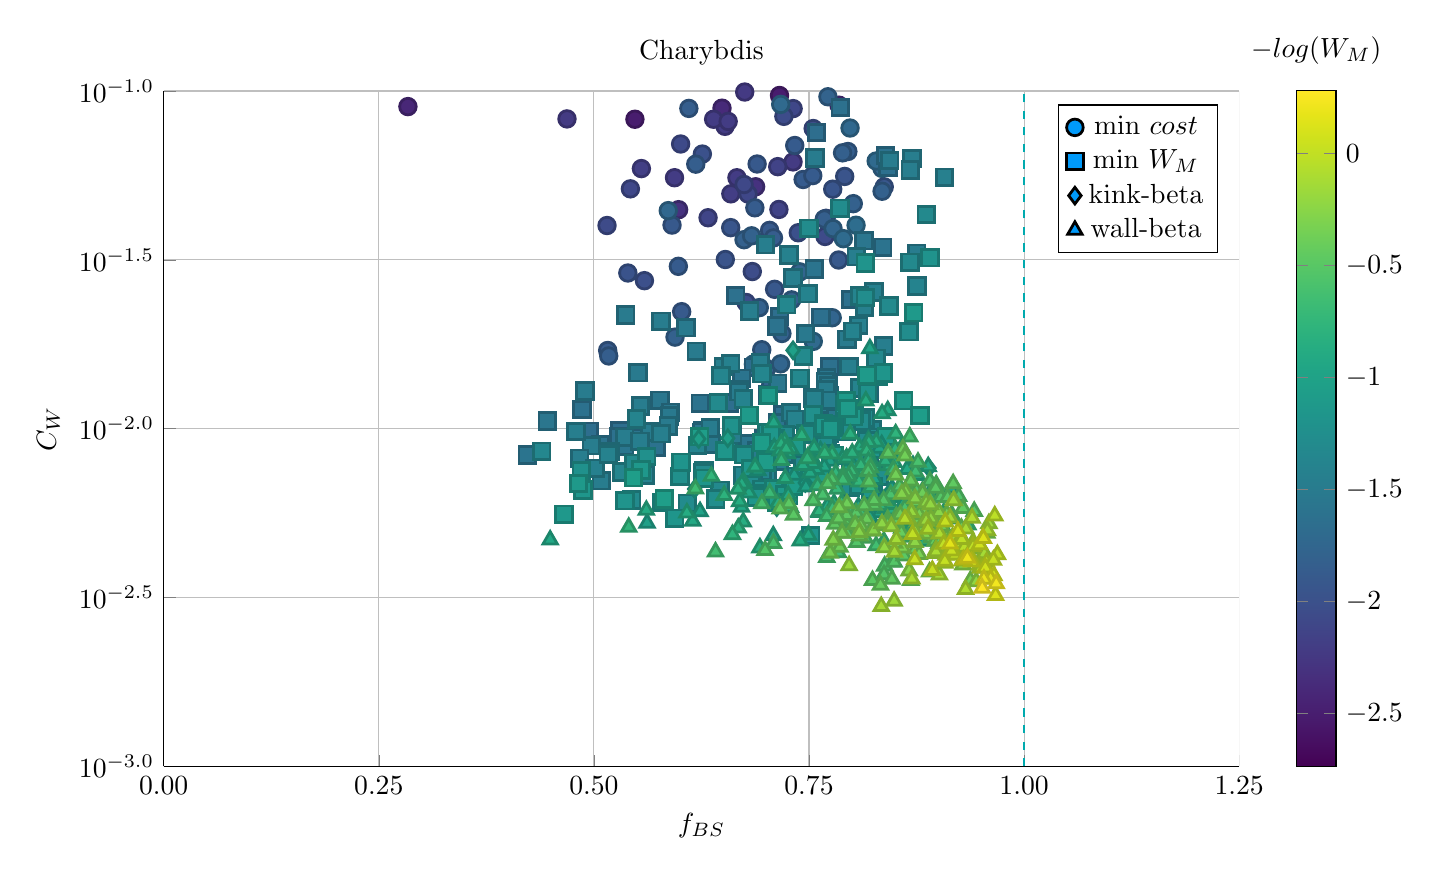
\begin{tikzpicture}[]
\begin{axis}[colorbar = {true}, height = {101.6mm}, ylabel = {${C}_{W}$}, title = {Charybdis}, xmin = {0.0}, xmax = {1.25}, ymax = {0.1}, ymode = {log}, xlabel = {${f}_{BS}$}, {unbounded coords=jump, scaled x ticks = false, xticklabel style={rotate = 0}, xmajorgrids = true, xtick = {0.0,0.25,0.5,0.75,1.0,1.25}, xticklabels = {0.00,0.25,0.50,0.75,1.00,1.25}, xtick align = inside, axis lines* = left, scaled y ticks = false, yticklabel style={rotate = 0}, log basis y=10, ymajorgrids = true, ytick = {0.001,0.0031622776601683794,0.01,0.03162277660168379,0.1}, yticklabels = {$10^{-3.0}$,$10^{-2.5}$,$10^{-2.0}$,$10^{-1.5}$,$10^{-1.0}$}, ytick align = inside, axis lines* = left,     xshift = 0.0mm,
    yshift = 0.0mm,
    axis background/.style={fill={rgb,1:red,1.00000000;green,1.00000000;blue,1.00000000}}
, colormap={plots}{rgb=(0.26700400,0.00487400,0.32941500), rgb=(0.27794100,0.05632400,0.38119100), rgb=(0.28291000,0.10539300,0.42690200), rgb=(0.28229000,0.14591200,0.46151000), rgb=(0.27619400,0.19007400,0.49300100), rgb=(0.26514500,0.23295600,0.51659900), rgb=(0.25042500,0.27429000,0.53310300), rgb=(0.23360300,0.31382800,0.54391400), rgb=(0.21813000,0.34743200,0.55003800), rgb=(0.20123900,0.38367000,0.55429400), rgb=(0.18555600,0.41857000,0.55675300), rgb=(0.17117600,0.45253000,0.55796500), rgb=(0.15772900,0.48593200,0.55801300), rgb=(0.14618000,0.51541300,0.55682300), rgb=(0.13374300,0.54853500,0.55354100), rgb=(0.12346300,0.58168700,0.54744500), rgb=(0.11948300,0.61481700,0.53769200), rgb=(0.12632600,0.64410700,0.52531100), rgb=(0.15014800,0.67663100,0.50658900), rgb=(0.19109000,0.70836600,0.48228400), rgb=(0.24607000,0.73891000,0.45202400), rgb=(0.31192500,0.76782200,0.41558600), rgb=(0.37777900,0.79178100,0.37793900), rgb=(0.45867400,0.81636300,0.32972700), rgb=(0.54552400,0.83803900,0.27562600), rgb=(0.63690200,0.85654200,0.21662000), rgb=(0.73088900,0.87191600,0.15602900), rgb=(0.81457600,0.88339300,0.11034700), rgb=(0.90631100,0.89485500,0.09812500), rgb=(0.99324800,0.90615700,0.14393600)}, colorbar style={title=$-log( W_M )$}}, ymin = {0.001}, width = {152.4mm}]\addplot+[scatter, scatter src=explicit, only marks = {true}, color = {rgb,1:red,0.00000000;green,0.60560316;blue,0.97868012},
draw opacity=1,
line width=0,
solid,mark = *,
mark size = 3.0,
mark options = {
    color = {rgb,1:red,0.00000000;green,0.00000000;blue,0.00000000}, draw opacity = 1.0,
    fill = {rgb,1:red,0.00000000;green,0.60560316;blue,0.97868012}, fill opacity = 1,
    line width = 1,
    rotate = 0,
    solid
}] coordinates {
(0.7359024750431782, 0.20372611777337152) [-2.737608795379803]
(0.5851953957160873, 0.16756698485075783) [-2.687028959846787]
(0.5364581048179937, 0.20307732356386315) [-2.590964172611572]
(0.7157155795294491, 0.09697011319422226) [-2.5133293798402634]
(0.5476668344586882, 0.08246486806905176) [-2.5100019193902536]
(0.5752437728161253, 0.19848215388453824) [-2.5025824444647777]
(0.7822657902821669, 0.18469850991270712) [-2.5011605733960924]
(0.7330176082872631, 0.12156262800516612) [-2.487146433631915]
(0.6068870363747878, 0.19851381203738652) [-2.4809660057819647]
(0.6590347940805605, 0.18516332132320687) [-2.470276837036607]
(0.2838228884486824, 0.08989325143911144) [-2.4120510478783452]
(0.5708561611145753, 0.11208716242840429) [-2.40064821683863]
(0.6846120659221104, 0.1197463715660703) [-2.3953673323479805]
(0.4540491134456154, 0.16126185747296792) [-2.393026566903574]
(0.664870722620742, 0.12157790627296668) [-2.3890711431592075]
(0.6488772614768177, 0.08892691625963052) [-2.3841714318705525]
(0.7962903980838778, 0.19098420146344375) [-2.3835230043455686]
(0.5527152139738948, 0.1567069747417994) [-2.381290315955617]
(0.5688566985496978, 0.12013460973440174) [-2.372431680776573]
(0.7534891693764634, 0.18909730733563926) [-2.3528250340145016]
(0.7848680602764574, 0.09075329244454268) [-2.3367870360584306]
(0.6786405769951752, 0.14161197175057597) [-2.321478568273318]
(0.6879316398295171, 0.05204568902739023) [-2.305558880403713]
(0.6025332208962126, 0.12356138844469775) [-2.304074016625784]
(0.5984321265445931, 0.04451265485552352) [-2.302767677581907]
(0.7386606591169115, 0.16063854506387298) [-2.296827704935537]
(0.6511502088521184, 0.10163604971512134) [-2.2875898578722627]
(0.7194233620171044, 0.11621384520807569) [-2.277792210835674]
(0.7567514313688793, 0.1663671711858832) [-2.2429196737605452]
(0.7579186381402687, 0.14065371048755002) [-2.2307023150334016]
(0.6752700403564966, 0.0992781716492562) [-2.229928759421221]
(0.7314415782128092, 0.06165765133592798) [-2.225497521252979]
(0.4687064864215902, 0.08264995845897197) [-2.2254079847151558]
(0.798488185414572, 0.10066936171865973) [-2.2222117952587324]
(0.7999537680483143, 0.11283696845057267) [-2.2164511971368666]
(0.6523833432801946, 0.07858675141449649) [-2.209080463460292]
(0.5936775460828698, 0.055353669168383704) [-2.209072102647127]
(0.639129584480767, 0.08246628156983182) [-2.2082284492074966]
(0.666208795279778, 0.05534045927382465) [-2.207545754633005]
(0.6560427480245121, 0.0812523499942961) [-2.2073960717358423]
(0.6591405401085446, 0.04959003498021099) [-2.1906798686881843]
(0.5551837247381063, 0.058916370946488036) [-2.180354292184896]
(0.7150132537788763, 0.04458441983079472) [-2.1445063804884623]
(0.7136491796753617, 0.05969099272190574) [-2.1441459472897755]
(0.6326692663477658, 0.04213154094480493) [-2.1211539010866085]
(0.7506892183015275, 0.11416954810746238) [-2.118865769548717]
(0.6791864978600942, 0.04953083435602705) [-2.0989534800462293]
(0.7315469652365952, 0.08867461574773429) [-2.098220502653117]
(0.6745347277267081, 0.0528553369774306) [-2.0935531757786148]
(0.5424055033322877, 0.05131047258257683) [-2.0908793980048204]
(0.6007799858607985, 0.06966107994211436) [-2.071206080374841]
(0.5152474997516242, 0.03996425224364798) [-2.064010547202469]
(0.7686026115092387, 0.03708750697043753) [-2.056677518407323]
(0.7207865714460837, 0.08410248770893317) [-2.046651526754166]
(0.6840849685675889, 0.029196081498388402) [-2.0379011758864283]
(0.7548350354881133, 0.07740613615195041) [-2.0346098603711273]
(0.6768336159103454, 0.023645385119135078) [-2.0286798881208097]
(0.5587072189827298, 0.027435451545116674) [-2.0136110022221563]
(0.7350235456977134, 0.11225395679162868) [-2.009422091461703]
(0.7375305044186223, 0.038038514881495206) [-2.0046094254929896]
(0.626054073537986, 0.06504727548043324) [-1.9998626026906214]
(0.5912300263829029, 0.1292818470624988) [-1.994011891463306]
(0.5394375501946231, 0.028908830411030862) [-1.9684875514336135]
(0.6527344577201069, 0.031694615819844695) [-1.962505769886516]
(0.7698840234200133, 0.041976164443053174) [-1.9620022465602456]
(0.7914883153195793, 0.0558374666834525) [-1.9556964151982232]
(0.7775684313579326, 0.051180643617204404) [-1.951439472922028]
(0.658985769190255, 0.03938689654476367) [-1.9407104232831573]
(0.8374522478389551, 0.05202238389928039) [-1.9285131737739916]
(0.7100254506306457, 0.025864965787053298) [-1.9158089273231942]
(0.7844213227435214, 0.0315876708787529) [-1.9026235632381945]
(0.5907921919303644, 0.04007799426592172) [-1.8998797107494547]
(0.6896895825351187, 0.06078277028813781) [-1.899469008660825]
(0.6019792525002452, 0.022206649532263138) [-1.8922403969034376]
(0.6914159704451317, 0.10343738795419383) [-1.8906275193753241]
(0.7041896502823766, 0.03865878413437627) [-1.888904730447693]
(0.5160181017136422, 0.01704724215883986) [-1.881726038777211]
(0.743187295487432, 0.05468787224768575) [-1.8763775212700056]
(0.7334309591956334, 0.06894730353059726) [-1.8735628617782005]
(0.5981394027328019, 0.030255781340376833) [-1.8728583861908288]
(0.7543798247443579, 0.05616340524751281) [-1.8726476950037667]
(0.6870514960504185, 0.04508699905590542) [-1.8707673950160981]
(0.7087125757213878, 0.036730885786441146) [-1.8559040168248113]
(0.6183905781152413, 0.06072120698828991) [-1.844735439552174]
(0.6103504198051167, 0.0887876180917983) [-1.8430067319432535]
(0.7951817179395599, 0.06618962633184258) [-1.8418706711323614]
(0.5172145933348372, 0.016421469596061083) [-1.839654971931263]
(0.7677643488639188, 0.041749778425302704) [-1.8363695553529753]
(0.6950647568960668, 0.017133631996777206) [-1.8261042714032643]
(0.7890113216319079, 0.06559232169922954) [-1.8156007183182272]
(0.8349557353351424, 0.050477285906930965) [-1.814915147975814]
(0.8014700349403633, 0.0463768454249938) [-1.8142470512570916]
(0.6922025322322042, 0.022826470712123872) [-1.8122133933822206]
(0.5942649107552632, 0.018671308945999422) [-1.8120480447424478]
(0.7298578035996299, 0.02406843511337114) [-1.810457309558868]
(0.6744865705831616, 0.03627504764978015) [-1.8068853182048894]
(0.7185012463149602, 0.019138039216325595) [-1.8019457667366159]
(0.6832930480165496, 0.03724912279904193) [-1.7968505393892884]
(0.7007625467971873, 0.015068032824050809) [-1.7952329403066731]
(0.8529644136574135, 0.10460346899306477) [-1.7847262081815998]
(0.7719812027452927, 0.09611727933154134) [-1.7840094275762153]
(0.7769681596557587, 0.021310065419317785) [-1.76773605949338]
(0.7393128324823182, 0.02913495659310822) [-1.7643358761825505]
(0.7056419712157331, 0.013537430460188857) [-1.7636964772599824]
(0.7169853719943156, 0.015563838196545969) [-1.7631697711543228]
(0.7779068969066241, 0.039135813481222324) [-1.7625125196445544]
(0.8348226277408363, 0.058991966200443106) [-1.7573515468471756]
(0.5863935693560001, 0.04422563848495237) [-1.7287980416000448]
(0.7977038871187261, 0.07767888704178068) [-1.7234251960549989]
(0.8280920948475081, 0.06204137364185275) [-1.706346162862732]
(0.7549772489845689, 0.018138423087163798) [-1.7045486732225623]
(0.7171125889592607, 0.09124971330207729) [-1.7014359592573747]
(0.7899075292932638, 0.0365316783828158) [-1.6927990438723723]
(0.6853958214714885, 0.015536674756802697) [-1.6898457437353114]
(0.804693703903259, 0.04003550886686569) [-1.6732846842044926]
};
\addlegendentry{min $cost$}
\addlegendentry{min $W_M$}
\addlegendentry{kink-beta}
\addlegendentry{wall-beta}
\addplot+[scatter, scatter src=explicit, only marks = {true}, color = {rgb,1:red,0.00000000;green,0.60560316;blue,0.97868012},
draw opacity=1,
line width=0,
solid,mark = square*,
mark size = 3.0,
mark options = {
    color = {rgb,1:red,0.00000000;green,0.00000000;blue,0.00000000}, draw opacity = 1.0,
    fill = {rgb,1:red,0.00000000;green,0.60560316;blue,0.97868012}, fill opacity = 1,
    line width = 1,
    rotate = 0,
    solid
}] coordinates {
(0.6851210809340392, 0.015197399614753464) [-1.6681264025020264]
(0.4941964393824304, 0.009823451646161325) [-1.663027891651841]
(0.530160434168107, 0.009846202245989184) [-1.6574639825902946]
(0.657378449413485, 0.011920058291303071) [-1.6569597902573525]
(0.7586216148428655, 0.07535163980234072) [-1.6567719329389001]
(0.7158310476944133, 0.02145281320442147) [-1.6490985707391912]
(0.7192558858327268, 0.010980468278747128) [-1.6422304847233504]
(0.7981807918170106, 0.024120165421292625) [-1.6325751861823363]
(0.7640459388499986, 0.021369208393676346) [-1.6291941426087102]
(0.8417754201260752, 0.059322254561326254) [-1.6271960977249518]
(0.7743051372156727, 0.015274978962504819) [-1.6270750467611084]
(0.664700618113425, 0.02479273110440336) [-1.626888156587228]
(0.7863682794539396, 0.08930149237460469) [-1.6249314455189936]
(0.5291119244133525, 0.009464726031912818) [-1.616950986036806]
(0.48595797227950854, 0.01140193486941599) [-1.6155813119347568]
(0.5723299817732307, 0.008812988458667981) [-1.6136190879018757]
(0.8388405409449038, 0.06439016913414505) [-1.6120765470743166]
(0.70226409417234, 0.012585512817446045) [-1.6084381516776733]
(0.7130021869125045, 0.02012839274260647) [-1.6020711217447665]
(0.5077104629720907, 0.008960652359910951) [-1.5956625490662]
(0.623540667348531, 0.011885919211945236) [-1.5936419030965376]
(0.8357083811774292, 0.03445722055743375) [-1.591719437101271]
(0.6974358183207425, 0.00935259758229712) [-1.5882416690043395]
(0.5494745058252606, 0.00941739351173858) [-1.587943800614445]
(0.4225576148062277, 0.008359730036220061) [-1.5878025494857624]
(0.7131882171897006, 0.010419937829338555) [-1.5868755906181577]
(0.7562368917045845, 0.029697190504060857) [-1.5849823271963874]
(0.6716640548925399, 0.014090253789926491) [-1.5820661333237485]
(0.6267086866070536, 0.009872769680224545) [-1.571414774494934]
(0.8140161912399068, 0.036055486397936085) [-1.561587842338199]
(0.6792373315387156, 0.009008401602884603) [-1.5604752308741954]
(0.44591630111536584, 0.010548811329102839) [-1.560024208321792]
(0.6253833131119283, 0.00975086483062938) [-1.5595172183929409]
(0.5357717637014691, 0.008877515881031174) [-1.5547403592804268]
(0.5767804998324492, 0.012128004524771618) [-1.5525172912757694]
(0.7804693216914177, 0.01075120106159998) [-1.550211325130473]
(0.7706256099884414, 0.01417054313300387) [-1.5499921130488996]
(0.7136233520662059, 0.013636547782905628) [-1.5488389310082484]
(0.5890435534060732, 0.01118682853182229) [-1.548636584215126]
(0.6960995570081354, 0.009004515948176011) [-1.5484303677563682]
(0.6891089745706832, 0.008589361734950092) [-1.5300696832010154]
(0.5877673649863151, 0.010918478084483) [-1.5240418415006989]
(0.7689373516155897, 0.013786535741271849) [-1.52035115860342]
(0.7458916933725457, 0.019102159289939535) [-1.5187095286365286]
(0.607104129340485, 0.019900882686515825) [-1.5152558703618486]
(0.7547906590532093, 0.01233142370653334) [-1.5130633149050525]
(0.6362345823351421, 0.008998649144966384) [-1.5127417843169062]
(0.727050378229241, 0.009033035828776036) [-1.512065872282441]
(0.5513544713967212, 0.014648425212785676) [-1.508698938344436]
(0.5368536810825235, 0.021717369003602268) [-1.5042599211378067]
(0.7620316566255821, 0.011787983533386965) [-1.5034350531454859]
(0.7725639125650813, 0.013402736400337721) [-1.50170709764633]
(0.681235287648052, 0.008403497514698337) [-1.501622468932281]
(0.6691676415273751, 0.013038942564365743) [-1.5014482706318735]
(0.7939788263529484, 0.018390392389316428) [-1.4999954524234758]
(0.6189955986913707, 0.01694354359189593) [-1.4973617780251773]
(0.5863662794504805, 0.010183371556613061) [-1.497105465512374]
(0.8436473841822292, 0.062282935043912684) [-1.4929511344473714]
(0.7571308398620893, 0.06324187033686292) [-1.4921349419619385]
(0.7738151286426059, 0.012548762978995496) [-1.4884591559674822]
(0.6686415918300896, 0.012867101009559307) [-1.487363796795517]
(0.4895966961882071, 0.012921001622500157) [-1.4866917975345906]
(0.6353463643428903, 0.010047951074758055) [-1.4840978906845892]
(0.8751665097475697, 0.03303866433608294) [-1.4824521913249147]
(0.8201318460604853, 0.012726704506142847) [-1.4821332841886103]
(0.5495938989749863, 0.007290805739373347) [-1.48122389777201]
(0.5651448258793007, 0.00977012454088988) [-1.4804970319589599]
(0.5085409731766444, 0.007020834402326414) [-1.4800609203732897]
(0.497047495750633, 0.008910343679206711) [-1.4785263901161534]
(0.7700846921982628, 0.013060328514041545) [-1.4759327339004988]
(0.6613546957182095, 0.009568901799246174) [-1.4716802129865878]
(0.5541661197172657, 0.011686646580567617) [-1.4714171457200942]
(0.5357853528313937, 0.009432683201513142) [-1.4697490463241623]
(0.5780574343855402, 0.0207896268155257) [-1.469182095495403]
(0.749496638108765, 0.00970055448692835) [-1.4669160574764228]
(0.7750171669992052, 0.009906198335664992) [-1.4650279037766998]
(0.48334514281038826, 0.008175296861755412) [-1.4649157170050158]
(0.8695060800287956, 0.06304537805517052) [-1.4637589731711664]
(0.8678168316150046, 0.058293696935902015) [-1.4637269213699509]
(0.6810497144003721, 0.022332692478256824) [-1.4633431723635995]
(0.553769872193598, 0.009175072172052877) [-1.4625771233357587]
(0.6993360633065318, 0.03507245292213848) [-1.4624493219359893]
(0.8048754097940412, 0.0323252483349636) [-1.456137936078477]
(0.7724185214963187, 0.012144991566364045) [-1.4552956920106896]
(0.47939065080719445, 0.009807429458519862) [-1.4545765412204814]
(0.83685598069093, 0.017552109366812733) [-1.4536933205355047]
(0.7008512611510139, 0.008376880643338882) [-1.4536264367612777]
(0.7313032608836818, 0.027928446404318328) [-1.4522195766945736]
(0.7965110041064016, 0.015275332383460013) [-1.4474663709891824]
(0.6932958919872281, 0.015700047070746036) [-1.4473086055649607]
(0.7730881776814797, 0.009670159078421467) [-1.4394573389116623]
(0.5779570147935796, 0.00966580645268258) [-1.43910869750835]
(0.8078038051086585, 0.02020398851625505) [-1.4359212547397637]
(0.715499444782145, 0.008025741974410725) [-1.4345455569874563]
(0.7208841307372137, 0.008395971364345037) [-1.4342039611389994]
(0.9074238589733309, 0.055516720625521446) [-1.431939711468657]
(0.5190051987619015, 0.008564631451482608) [-1.4318393301192203]
(0.6504475928061844, 0.015286328537971657) [-1.4298782830268841]
(0.7292085089618878, 0.011144326549623773) [-1.4297531319990848]
(0.81448792065999, 0.022836013108600235) [-1.429493152311542]
(0.825574988161768, 0.02541733792453219) [-1.4257656907023994]
(0.501465121842191, 0.007637958943877289) [-1.4246908118870814]
(0.7266226606300097, 0.032702505993041836) [-1.4223151615986427]
(0.6591067142233716, 0.015605848032644089) [-1.4209285260987674]
(0.5167081891349604, 0.00838874188644035) [-1.4103191250155003]
(0.5596505617132486, 0.007287678962320866) [-1.409160412241362]
(0.7557455862541304, 0.012263516831132143) [-1.3987487890322283]
(0.7341248325017325, 0.010656632838165833) [-1.3961077718749653]
(0.8092287508171119, 0.013186567390631069) [-1.39553831950318]
(0.8203576874800285, 0.00805251109990194) [-1.3921916689745937]
(0.8004943813587586, 0.019423304332311736) [-1.391977480132208]
(0.7489120391350832, 0.025114205055596032) [-1.3910450519688433]
(0.8754057461611234, 0.026458278303411537) [-1.3854794296349102]
(0.6735716252835262, 0.012247975078154037) [-1.3835251244626703]
(0.7665028038099523, 0.008921077760690099) [-1.3812630274600655]
(0.7015621857164597, 0.007416332681742631) [-1.3791460184166777]
(0.6202964877938695, 0.008932161350486465) [-1.376877777579119]
(0.8087590580422906, 0.024683476432383993) [-1.375791428631395]
(0.5494124765358024, 0.010670268336180793) [-1.3747828318073587]
(0.8149159088702812, 0.007870433585163046) [-1.3692376523933565]
(0.5320990994872573, 0.0074378152848894735) [-1.3684330757581267]
(0.7481734016173558, 0.008098566001726598) [-1.3642308788975135]
(0.6476576358282994, 0.014345667909698757) [-1.3639106630352087]
(0.6558906704773511, 0.008572986953587419) [-1.3552608297970883]
(0.8237471775593819, 0.00992037446225701) [-1.3550143961305745]
(0.7982100921053328, 0.007328347073490059) [-1.3536632792649093]
(0.6953629282134552, 0.007510901593863939) [-1.3520272957429909]
(0.6953230050470768, 0.014541602438699657) [-1.3510576974042412]
(0.6730211677715083, 0.007284218364658594) [-1.3496042220443973]
(0.7239679168228259, 0.023274179527198832) [-1.341589260669594]
(0.4393956478215161, 0.008576558289309913) [-1.3400141478767358]
(0.7426807786520446, 0.00783880949696723) [-1.3300314493551002]
(0.7395236873382182, 0.01411038207207742) [-1.3284263237560021]
(0.684855303548374, 0.007486503783717723) [-1.3242939338468662]
(0.8278021824532116, 0.016172436730796002) [-1.323178727777929]
(0.627797840186422, 0.007515284989600465) [-1.3213550729926942]
(0.8674653533336951, 0.031083172357107024) [-1.3188753969554132]
(0.6467532218081451, 0.006572813918743706) [-1.3138992633454782]
(0.8864160782387862, 0.04309583371292883) [-1.3112533972207423]
(0.6269156989625477, 0.007413444843148486) [-1.3066175516543825]
(0.8431393595924693, 0.02306836377257982) [-1.3040612288627607]
(0.8197076367002643, 0.00943254285754032) [-1.3038133693852783]
(0.6445239701337245, 0.01190899263404481) [-1.301084703290134]
(0.5463650306744098, 0.00789699984651379) [-1.3010145120900876]
(0.5437906828898529, 0.006149219434619409) [-1.3000605956773916]
(0.7434166628060613, 0.016437005811172183) [-1.2981699890610565]
(0.7146749298387812, 0.008660055713531614) [-1.2951558801969907]
(0.8148780528301931, 0.010749954823506654) [-1.29444309797184]
(0.6084531928479563, 0.006015009649024556) [-1.2856101424882644]
(0.7220256115514188, 0.009584357937856927) [-1.285263592011844]
(0.7859463410460376, 0.04494124949431044) [-1.284383793501614]
(0.799675832204197, 0.00683431321635412) [-1.2828114288158374]
(0.7499713034119133, 0.039187382342347976) [-1.2826431650359629]
(0.734351532241878, 0.007231700278305266) [-1.2824255065429995]
(0.713445223919135, 0.00853616645957665) [-1.2813323109549335]
(0.790122159696273, 0.006837657402697755) [-1.2806421539894215]
(0.8175324002405339, 0.009211465915111147) [-1.2790915578265545]
(0.8109413385537045, 0.010542099378207213) [-1.2707451840708122]
(0.8154085690878763, 0.024447750750697092) [-1.2676539939434082]
(0.771441058879269, 0.009098409772603787) [-1.2653553126366786]
(0.7976978951094078, 0.006725537497980498) [-1.264293982211982]
(0.8663731578909948, 0.019363431367524053) [-1.262045130852001]
(0.6826626081076077, 0.006906076996276599) [-1.2611290819783112]
(0.7930953306749782, 0.009803145458874337) [-1.2555987795426622]
(0.6414699980625864, 0.00619895569247597) [-1.2513270179335647]
(0.8316118369664839, 0.007239853513876978) [-1.2453167838780697]
(0.7681268084076656, 0.008896586162085272) [-1.2430939343579344]
(0.7009518612475429, 0.009719593902466845) [-1.2381773742332136]
(0.5613695492397395, 0.008270424440644015) [-1.2346782486332617]
(0.60010992732849, 0.0072241626571935376) [-1.2264046023709216]
(0.7548991538536438, 0.01098843719538726) [-1.2247195887884887]
(0.7269708164874584, 0.006808974225612837) [-1.2180889658059086]
(0.6946997618970708, 0.006611305121542242) [-1.2173874089477876]
(0.48544389569163865, 0.007501419726936573) [-1.2146247722956514]
(0.7909335635528599, 0.011764386053045915) [-1.2132972156104522]
(0.6745620250506631, 0.008378063320530003) [-1.2109120215395388]
(0.7747592904603993, 0.008427299987451904) [-1.2084181738286368]
(0.8180761130344034, 0.01273555061242485) [-1.20714909048448]
(0.6600048470179246, 0.010213320377511352) [-1.2033520253557135]
(0.8904893803598241, 0.032086426450625864) [-1.1973567207367808]
(0.7794460337871526, 0.01024990923611188) [-1.1946911954531152]
(0.7685171934523852, 0.010020735618058307) [-1.194687477055283]
(0.74643037518658, 0.009634752809511687) [-1.1937967228670217]
(0.8305632837722567, 0.014319974319254046) [-1.185724861965876]
(0.8154688896102296, 0.030946696104817876) [-1.1815951507377263]
(0.5359199492602275, 0.006119538485938838) [-1.1806237088701466]
(0.5790003431047352, 0.0060467130253046425) [-1.1800813312023146]
(0.6010234873787892, 0.007952378649071718) [-1.176244530950471]
(0.6903543708921169, 0.006432608194369421) [-1.1748225292203367]
(0.5938066341086683, 0.005427058328431804) [-1.1721208310483742]
(0.8244672749127927, 0.006744537821609478) [-1.1717373686057835]
(0.7520366981220118, 0.004828891223049449) [-1.1708649361692889]
(0.8079347587629624, 0.006810003648499363) [-1.1692163263768098]
(0.7113020735368382, 0.009353534353065332) [-1.167353919317699]
(0.8366541770603382, 0.014618785296867573) [-1.1652399164280889]
(0.8261711137782428, 0.008829535690276422) [-1.162809974145342]
(0.6281137770625854, 0.007136024429485349) [-1.1600693635040116]
(0.48744515553761025, 0.006579111152003091) [-1.157321108695414]
(0.651991884299557, 0.008599780741533768) [-1.1572067562856314]
(0.7107092242352311, 0.009251618906581017) [-1.1571634670399211]
(0.8088839694703398, 0.008133610271699837) [-1.154357334346231]
(0.8027929243249681, 0.011084851654264415) [-1.1506586644938104]
(0.823695688879586, 0.008713510430388705) [-1.150227655836216]
(0.822008562445382, 0.006602548762005154) [-1.1491924102402016]
(0.688612348505278, 0.006272419326365313) [-1.1477835171917188]
(0.6820414615312915, 0.007620679601131938) [-1.1465058315496728]
(0.7665548771358827, 0.010377192915174936) [-1.145014274974487]
(0.705868708485792, 0.009696220536212618) [-1.1375870233869183]
(0.767634347550663, 0.010180634102852183) [-1.1373650551215082]
(0.5547128257478453, 0.007542730978334406) [-1.1357458790371815]
(0.7783986920955023, 0.010126349397671063) [-1.133986432515703]
(0.4651362590200956, 0.005578205050921048) [-1.1320341014158335]
(0.8015228446950137, 0.010846318354017281) [-1.127079592692178]
(0.726461760542858, 0.006331906889150134) [-1.1252988863479554]
(0.48208147962640285, 0.006879141460401252) [-1.123003263844327]
(0.8717607864580118, 0.022040928898795047) [-1.1207682191899027]
(0.774982528534528, 0.00996173564893061) [-1.1180749050851169]
(0.7093096094323664, 0.006626896988025552) [-1.1159299024060154]
(0.8171791685966094, 0.014399132022875615) [-1.111366047368976]
(0.7932954390046818, 0.01206983625295502) [-1.1093461418096882]
(0.7219772506321358, 0.006356432017833017) [-1.1083223146390213]
(0.7029191591245791, 0.012535144034281957) [-1.108020004377878]
(0.7346977255426123, 0.00883860338226376) [-1.1055395253528022]
(0.6805779282507709, 0.010954609847675004) [-1.1018087579792433]
(0.7375539791268741, 0.006955673427821012) [-1.1000312304906807]
(0.7953037368390077, 0.011476323196829152) [-1.0958683903566835]
(0.8599427472738629, 0.012099180088161502) [-1.0918611830445206]
(0.7644072104571058, 0.007324655445979312) [-1.084008635561983]
(0.779650226067546, 0.008347799057721199) [-1.0818442729737123]
(0.6998274928068458, 0.007973263522900845) [-1.0762205003226006]
(0.87917336532856, 0.010946001598484297) [-1.0742112770850791]
(0.694879746234392, 0.009087852412631436) [-1.0708769548182164]
(0.7321698469384964, 0.0067597442860644836) [-1.069695292943837]
(0.545938699421471, 0.007160447099405331) [-1.0603710996179994]
(0.6228473762742924, 0.009473258949863166) [-1.058639833713732]
(0.5819104753803194, 0.0061899243692649306) [-1.0559914680496412]
(0.8398342477938563, 0.009482529791919412) [-1.0537452246128203]
(0.7506931030637808, 0.00708059455566661) [-1.0532767994986825]
(0.7126332937977515, 0.006035560775312132) [-1.0518252532905286]
};
\addlegendentry{min $cost$}
\addlegendentry{min $W_M$}
\addlegendentry{kink-beta}
\addlegendentry{wall-beta}
\addplot+[scatter, scatter src=explicit, only marks = {true}, color = {rgb,1:red,0.00000000;green,0.60560316;blue,0.97868012},
draw opacity=1,
line width=0,
solid,mark = diamond*,
mark size = 3.0,
mark options = {
    color = {rgb,1:red,0.00000000;green,0.00000000;blue,0.00000000}, draw opacity = 1.0,
    fill = {rgb,1:red,0.00000000;green,0.60560316;blue,0.97868012}, fill opacity = 1,
    line width = 1,
    rotate = 0,
    solid
}] coordinates {
(0.834626495849728, 0.006083501631057066) [-1.0496814932160978]
(0.6170409460102284, 0.006629793134010975) [-1.0478282176510978]
(0.8894694614486488, 0.00764908073743482) [-1.0476862508436227]
(0.7124945816098436, 0.005862884354721373) [-1.0434060376287386]
(0.6218172305989085, 0.009322710512378526) [-1.042586757918211]
(0.8441447569005192, 0.006487752068877104) [-1.0395059774095508]
(0.6555943522609418, 0.009374281366493263) [-1.037130039873791]
(0.7314329599011424, 0.0170614588554745) [-1.0308313508546258]
(0.745698806783015, 0.006913114243597262) [-1.0275590312193816]
};
\addlegendentry{min $cost$}
\addlegendentry{min $W_M$}
\addlegendentry{kink-beta}
\addlegendentry{wall-beta}
\addplot+[scatter, scatter src=explicit, only marks = {true}, color = {rgb,1:red,0.00000000;green,0.60560316;blue,0.97868012},
draw opacity=1,
line width=0,
solid,mark = triangle*,
mark size = 3.0,
mark options = {
    color = {rgb,1:red,0.00000000;green,0.00000000;blue,0.00000000}, draw opacity = 1.0,
    fill = {rgb,1:red,0.00000000;green,0.60560316;blue,0.97868012}, fill opacity = 1,
    line width = 1,
    rotate = 0,
    solid
}] coordinates {
(0.561781693172161, 0.005256053052710575) [-1.025114084474608]
(0.7328778253267054, 0.007284527271346537) [-1.025064662372027]
(0.8007534210560534, 0.00782078493256419) [-1.0135716419780334]
(0.8262131393427226, 0.005878041854646887) [-1.0133032391552028]
(0.6905506855070277, 0.007516810149579491) [-1.0129395602075102]
(0.8321644284749603, 0.005642606316680264) [-1.0090683465802397]
(0.7950726411527982, 0.007590586049588419) [-1.00487994972194]
(0.7745441322154459, 0.008018904893245096) [-1.0024486517409639]
(0.6233290112259804, 0.005687012650490601) [-0.9982503197852052]
(0.8207534028698369, 0.017272851302606376) [-0.9980863049007114]
(0.8345152086201154, 0.008976011549139531) [-0.9976413099828907]
(0.7463634982112085, 0.00672377146821775) [-0.9952427135597887]
(0.8372618582030043, 0.006179152610909006) [-0.9882704184280687]
(0.8464783361909116, 0.006658577387207133) [-0.9865959618907963]
(0.7633220600898417, 0.008611185683760977) [-0.9861502224644026]
(0.7552278550565529, 0.00861006159819778) [-0.9834884062410291]
(0.8264185188855481, 0.007078972975952707) [-0.9755470230412873]
(0.7923915340714205, 0.007165169234302644) [-0.9751682968759733]
(0.8074567550650718, 0.00588288059860778) [-0.9745460269854277]
(0.8318914609825181, 0.008762707263760248) [-0.9724510296030006]
(0.8213035185218059, 0.0054508764537053) [-0.9721723790112873]
(0.7930318484620907, 0.007500206088288035) [-0.9683079871351761]
(0.8188945200120549, 0.00925430650881406) [-0.9640479639625688]
(0.767842670848498, 0.007713542274813112) [-0.9605456904465843]
(0.7096157753674764, 0.008793232884908199) [-0.9509475064598062]
(0.7580155421129163, 0.00758530046831779) [-0.9475613034981963]
(0.7089024870209081, 0.010432599107525612) [-0.9431073279051986]
(0.9149131868692663, 0.006669463740427501) [-0.9395228095882537]
(0.4491718650706183, 0.004688262944849126) [-0.9379797386819722]
(0.6716296429821872, 0.005855680709409532) [-0.936956260188316]
(0.7084973783953123, 0.004823068577046762) [-0.9328401416066296]
(0.8473084623363518, 0.006257853989784519) [-0.9307108052550614]
(0.680102277451425, 0.006461854726339168) [-0.9281558619803609]
(0.7286173554216664, 0.008735963170322575) [-0.9264995775599043]
(0.6148265392179618, 0.005328057424477724) [-0.9262426999191099]
(0.8708623476098649, 0.007790932759723544) [-0.9227003718927437]
(0.7511842078366924, 0.007406866683715918) [-0.9211202387251416]
(0.7492906727437184, 0.004842693465206878) [-0.9122780994598872]
(0.7955701829594555, 0.00553456744660005) [-0.9098639973117462]
(0.7558381020157489, 0.00799774423691871) [-0.9085892171866993]
(0.8415001071316417, 0.011322447729645281) [-0.9043705523492929]
(0.7890506006382549, 0.008178982728725071) [-0.903352069757217]
(0.7712915128293827, 0.0058981820527739225) [-0.9005612951337819]
(0.7258140216436932, 0.006353815969057234) [-0.8985196847828957]
(0.5609209176660367, 0.005739892493181049) [-0.8983797144291398]
(0.8639203180223186, 0.007583618995886536) [-0.8971261027713628]
(0.8607562916265183, 0.006081355532545074) [-0.8962149920198969]
(0.754373466724369, 0.007895141300507174) [-0.8947574466288085]
(0.7247460265098778, 0.008446442250875192) [-0.8916300803179569]
(0.8160520408511582, 0.012086236110976131) [-0.890947883956792]
(0.8885362197506304, 0.007728598763745398) [-0.8865999168444305]
(0.6739713276486742, 0.006968625853256571) [-0.8862290860463612]
(0.6718514222391598, 0.00686791587727973) [-0.8853692596179883]
(0.8349391514029897, 0.011077289150155845) [-0.884029767456243]
(0.8386840624601364, 0.005982150284429834) [-0.8837850767800522]
(0.7926189511510549, 0.007098671990886852) [-0.8828563557879437]
(0.8755325354782295, 0.0072796273438267495) [-0.8804549747402444]
(0.7429355983125893, 0.007792003070402551) [-0.8799662830695792]
(0.6873358671749346, 0.007704064980519725) [-0.8744133357565225]
(0.608078559277003, 0.0056363780626130485) [-0.8730986298376362]
(0.8650491065103372, 0.004988178616679241) [-0.8728030894608018]
(0.755949029174458, 0.008770502666972253) [-0.8727320299344076]
(0.7164979559318809, 0.008601244202966506) [-0.8720334149277572]
(0.7397597050644923, 0.004655770362479482) [-0.8693487943882443]
(0.6693564574335278, 0.006084065906903396) [-0.8630202034214742]
(0.8948336018025309, 0.004924842040843803) [-0.861299793442028]
(0.6735677102568205, 0.005298172414294102) [-0.8595038240809204]
(0.884070817557377, 0.0046473625238345456) [-0.8567854750862633]
(0.8392200926952157, 0.005815101976145971) [-0.8560196956809655]
(0.8086377049101, 0.008787976150626518) [-0.8549409997795642]
(0.7620585480612541, 0.005657937584887749) [-0.8549130093089008]
(0.721608466453812, 0.00917703801839012) [-0.8535716907113037]
(0.8574731878954547, 0.008347881751030625) [-0.8521148893133685]
(0.7223023329248925, 0.007128967537191795) [-0.848258534769848]
(0.828082086272923, 0.009136355586300991) [-0.8460593767435973]
(0.8914338433470699, 0.006518603909074656) [-0.8436096023361083]
(0.7790818338019714, 0.006010163492689091) [-0.8427994583004987]
(0.8489823330394292, 0.007945945585113466) [-0.841947416622939]
(0.7140164502630464, 0.0060248058000312785) [-0.840612447094069]
(0.692960158641591, 0.004440943928455613) [-0.840512586473128]
(0.7936846601062392, 0.008192611227802852) [-0.8396933257766793]
(0.8253036422768626, 0.007794162811523137) [-0.8357637262102798]
(0.7176577445146243, 0.009012091589396549) [-0.8345082268411569]
(0.8411026749122155, 0.008170154991858254) [-0.8326261675235949]
(0.8673453392641903, 0.006937374865533122) [-0.8320882392153445]
(0.8443535134063129, 0.005749714926123568) [-0.8315762378530004]
(0.6674327583656098, 0.00662694635784487) [-0.8307347851507457]
(0.7979229568222829, 0.009642717688792466) [-0.830544413041331]
(0.7486196493214454, 0.008249655917762508) [-0.8297213382977437]
(0.7234408795670257, 0.00872151277844613) [-0.8286741188165131]
(0.8195077166471576, 0.009115953893059449) [-0.8267848509238259]
(0.7415863096812476, 0.009559156785738465) [-0.8225460718617404]
(0.882628421673329, 0.005739050504125615) [-0.8214723162104086]
(0.8441514595814047, 0.00777900336077081) [-0.8201412806434945]
(0.8002081668892973, 0.008465745314703852) [-0.8151576039795889]
(0.6677669744096973, 0.005082760625336129) [-0.8142249848207472]
(0.8388338734372748, 0.008019437945510303) [-0.8140641213229001]
(0.844349544914433, 0.005973868428211905) [-0.8103019758142813]
(0.8655797889605916, 0.0048937089468515296) [-0.8012431956657198]
(0.8767235956859443, 0.005621145192877696) [-0.8003481799777136]
(0.6514463008690072, 0.006353153460386551) [-0.7977579467571502]
(0.7768358242558124, 0.008421833334043108) [-0.7930251215824343]
(0.8131055308236846, 0.007429093264895125) [-0.7890451923079399]
(0.8577409198580296, 0.008826772268823495) [-0.787865286509519]
(0.8571117381670891, 0.006383916218566666) [-0.7843040366780064]
(0.7617613692882175, 0.005696794743220581) [-0.7839186276792087]
(0.8399957501289924, 0.006115696804857897) [-0.7832803335041352]
(0.9154813470712311, 0.005413509713037376) [-0.7821184247172652]
(0.8169552335864975, 0.008596617727968549) [-0.7805782205003577]
(0.8507297272541241, 0.009659872283801132) [-0.7798419979328133]
(0.7480474290724733, 0.008159117975808313) [-0.779526126485372]
(0.8190855489333428, 0.00801636696090187) [-0.7754633993416067]
(0.7683076772552567, 0.008468144805643287) [-0.7736782567370082]
(0.8036381327462332, 0.007247388825611958) [-0.7730881104428101]
(0.6609890516858297, 0.004861686496363432) [-0.771875090323587]
(0.8208529541828645, 0.005934301325116477) [-0.7684162906476206]
(0.857888157512953, 0.005077595748671911) [-0.7679743247932476]
(0.7599118957144253, 0.006786674226710283) [-0.7648185888526707]
(0.5404722311866441, 0.005109733182186724) [-0.7640789887074095]
(0.850303323221387, 0.008706119585241447) [-0.761342175922955]
(0.8324703962569376, 0.005941882664679825) [-0.7543127087245246]
(0.7810180143390126, 0.007371584809935278) [-0.7536484511278393]
(0.6365120126946172, 0.007235631321785017) [-0.7503956953450397]
(0.8102664427840746, 0.007794584633403252) [-0.7487808552191573]
(0.7179080344472686, 0.008059650365173391) [-0.7476061772087611]
(0.8081839139783411, 0.006963610302502873) [-0.7471256555265617]
(0.8215135890335709, 0.006698880656946609) [-0.7413304463691416]
(0.906510252238872, 0.005641975327508916) [-0.7367054574686347]
(0.7879258843595898, 0.006032870871331476) [-0.7331219552552337]
(0.7827283817945546, 0.006626912607429937) [-0.7143600945963312]
(0.7993934646487343, 0.007474831733495699) [-0.7106398428950327]
(0.8887316474556182, 0.0049761893476396495) [-0.6960873863412442]
(0.881376398190137, 0.005409555517719824) [-0.6958903955949629]
(0.7284595482955875, 0.005844386265058715) [-0.6930492540076382]
(0.7771753343842193, 0.00580869705512685) [-0.6929516890222392]
(0.9346631437744438, 0.005195474212399125) [-0.6915921881710438]
(0.7042690087414297, 0.006450299363758911) [-0.6857195379800745]
(0.7957275168756369, 0.007235955498415392) [-0.6856480650317041]
(0.7897107828861115, 0.007277002386326683) [-0.6825231692879921]
(0.7973600098611778, 0.005826409813708321) [-0.6799325504597861]
(0.784228905597579, 0.005748438997690529) [-0.6756496749536086]
(0.8370184847542357, 0.004642372121698665) [-0.6668421547656437]
(0.7893582740009938, 0.0070613972149505) [-0.6594486343899455]
(0.9040400511046615, 0.005204006670639966) [-0.6592191769587943]
(0.6179292248677679, 0.006638640066368149) [-0.6536209377575128]
(0.8480642947896218, 0.007561107269230883) [-0.650948550154174]
(0.8737967946784376, 0.0074536379991662315) [-0.6505954513533947]
(0.8104512110396144, 0.00562511440860501) [-0.649384718466127]
(0.7872802988853757, 0.0056379604361593005) [-0.6434610863211887]
(0.8727513962004305, 0.004893302789367808) [-0.6386314300711667]
(0.8816223373482828, 0.006520915492483144) [-0.6385156325462752]
(0.7840350618679737, 0.004295648023998173) [-0.6376426431852426]
(0.6413221738351599, 0.0043195416112934695) [-0.63745836942971]
(0.8280408116192789, 0.004504479712425151) [-0.634161727858793]
(0.770629091366626, 0.00550347046899009) [-0.6307004133850902]
(0.8214244494729275, 0.0076645781815444635) [-0.6183303859395417]
(0.8651481856574186, 0.004777548127961022) [-0.6130870829164431]
(0.7962746747618027, 0.005139848231321853) [-0.6129648030838463]
(0.8671409497325202, 0.009455939774823839) [-0.6084696230229766]
(0.6952012284346729, 0.005998204689845081) [-0.6069152599086628]
(0.8912308167445621, 0.006234008404953501) [-0.6054076068022625]
(0.8712898879417955, 0.005960524285263344) [-0.6024296737568321]
(0.7706299004977172, 0.004158248718194877) [-0.6015484963981724]
(0.8977757862883986, 0.006792484353594769) [-0.6012984238357434]
(0.7997545861464158, 0.0053623804243832325) [-0.5960707607608329]
(0.7659594279780312, 0.006374522460113841) [-0.5936136176179417]
(0.8766607778850557, 0.007967211841028115) [-0.5931302760876686]
(0.846288022283653, 0.0040369634147211595) [-0.5915885524237119]
(0.8686741183403025, 0.006918880590157332) [-0.5911727158362008]
(0.7087237194035546, 0.004576324737559804) [-0.5900682137185816]
(0.8186632676533585, 0.0074842396419395755) [-0.5884302817228046]
(0.7900183388819731, 0.005019503207090587) [-0.5877411509443977]
(0.8449348419583856, 0.006377695642268969) [-0.5867809186460089]
(0.8894386439718743, 0.005390939798069345) [-0.5825897309583699]
(0.861458778960287, 0.005822320038436803) [-0.5801191442990684]
(0.7765230116766165, 0.007078947827278213) [-0.5723010609292049]
(0.8930353233119908, 0.004797737450304729) [-0.5679221681687051]
(0.8152095416974562, 0.004745752868187461) [-0.5631840336886528]
(0.8379455009974563, 0.00392267122135458) [-0.5608362242209843]
(0.8905134159362131, 0.0069992567132512) [-0.5571205537040459]
(0.754839738401019, 0.006126321093742513) [-0.5485242916279889]
(0.77159018447825, 0.006874419461623871) [-0.5418068538132612]
(0.8978282334851548, 0.006822436837333278) [-0.5416427697741687]
(0.8815859891084225, 0.005644924884791849) [-0.5402605106654789]
(0.8553304998012851, 0.0067352955911504) [-0.5386131387961719]
(0.9239134830651885, 0.006300681826786258) [-0.5359571495451664]
(0.6988911750990952, 0.004361609192009016) [-0.535080858548875]
(0.8055259375096102, 0.004607755561392721) [-0.5306887960741941]
(0.8367259402516638, 0.0061242176982959935) [-0.5279445193313689]
(0.8748863967569592, 0.005699821777253932) [-0.5261185431060132]
(0.8371729333582552, 0.0036996967788339836) [-0.5222207530468324]
(0.8488949558629858, 0.0040283964244842855) [-0.5213443855242413]
(0.8749285008369249, 0.00654764695467552) [-0.5183202512122866]
(0.9158953519092266, 0.005565518290350856) [-0.5127600710400247]
(0.9031002442664525, 0.006257154173968822) [-0.5093311143657722]
(0.8790111178540976, 0.005081917135024615) [-0.5092608114367078]
(0.8045809142404459, 0.005634560391700447) [-0.5060145289105423]
(0.9420096803870313, 0.005696558547132009) [-0.4991936251195474]
(0.8196674588798039, 0.006963136499419175) [-0.4985513425302997]
(0.8257700225656487, 0.005936448000755268) [-0.49568499824767104]
(0.9153141979650739, 0.005499933154622071) [-0.49145223309081343]
(0.7909072663757235, 0.005365451873400001) [-0.489720395145329]
(0.7940227144675952, 0.00491035857559783) [-0.48946631183449096]
(0.7320787810157223, 0.005551912726236007) [-0.4844323986419559]
(0.8927497803271689, 0.004748719229574022) [-0.48348457652780674]
(0.8420010977641849, 0.008465503287908559) [-0.4828289975574789]
(0.9110449050232763, 0.006257332981884576) [-0.4809853618707981]
(0.86039695942421, 0.004200694755861984) [-0.4809735664575194]
(0.7265808068427371, 0.0059994354167316145) [-0.4808665748655182]
(0.8238098981143183, 0.003555536540962884) [-0.47941962356708046]
(0.8972231176808156, 0.0066692846879273) [-0.47870566324028313]
(0.8256400317835417, 0.006131865359849344) [-0.4657796688745686]
(0.8686293024747704, 0.006395516513040164) [-0.46371269394589404]
(0.8514644923481995, 0.005496536453572034) [-0.45939503859612524]
(0.7799019216828753, 0.005214384126637902) [-0.4580684801880486]
(0.7938394409052723, 0.0055399395484132434) [-0.4551930791506963]
(0.8464021941983755, 0.0035852448301646562) [-0.4548470636638538]
(0.9175291713709409, 0.006879940028304696) [-0.4511448351238025]
(0.8141188915667769, 0.005918008902458026) [-0.4506410472161431]
(0.9009640556412939, 0.005592591526077269) [-0.44462955271421334]
(0.7163979727195185, 0.005788664224478401) [-0.4417671924951601]
(0.8505177854313649, 0.00532175252277852) [-0.44063870628617696]
(0.8920869625339607, 0.005848263216255258) [-0.437792328306716]
(0.8413875479481865, 0.005381947350223633) [-0.4372128319808473]
(0.9289177551894326, 0.005807357934085231) [-0.43652773545054785]
(0.8682949722579286, 0.0035579027524431407) [-0.4353218816843834]
(0.7843097302577535, 0.005420864551162702) [-0.43301226198144244]
(0.8964830647760125, 0.004646937579329881) [-0.42496774176553237]
(0.8745426212493882, 0.006054896100373839) [-0.4234566027757057]
(0.8414632584737313, 0.005209006616931108) [-0.4201824434096411]
(0.8682872105207565, 0.007002732156807032) [-0.41942034556894325]
(0.8573424977816416, 0.0049133604129482904) [-0.41625636474955513]
(0.8212694674949965, 0.004976224512696799) [-0.4153472596885677]
(0.8330587016869412, 0.003443555856640112) [-0.413698533116882]
(0.9010449971024423, 0.004578061980750892) [-0.40716887268106433]
(0.8737702130691167, 0.004403076051908361) [-0.4054968032106688]
(0.8169925126444579, 0.005401731740408723) [-0.4052996247784937]
(0.8759172148862289, 0.005310951805886482) [-0.4028975857602535]
(0.8591367153039695, 0.008698035154467071) [-0.39012186383455005]
(0.8560617406515993, 0.005569688147985928) [-0.3893599374140784]
(0.881963623925512, 0.006443553450960519) [-0.3874731327472749]
(0.7805343997879001, 0.004467008080186493) [-0.38658238651008303]
(0.7859678282204032, 0.004460761734980448) [-0.3844088155607324]
(0.927107662864025, 0.005076162944946042) [-0.3841297559869705]
(0.8088001349045256, 0.004818082688701254) [-0.3799233329958369]
(0.7940920333223207, 0.005997359653275597) [-0.37864836021510145]
(0.8101992223388763, 0.005149154541509343) [-0.36993435073896774]
(0.8614894682048851, 0.008306174738593903) [-0.36922049805921237]
(0.8036344625940746, 0.005209314390453537) [-0.36517136675970174]
(0.8508628415378322, 0.007290638437768607) [-0.36363162472662647]
(0.9616677715876509, 0.0036256611613784515) [-0.3560282417598354]
(0.7850672781503891, 0.005842256453254562) [-0.3516846326479429]
(0.7884853903565926, 0.004905016792320226) [-0.3492105588330574]
(0.910169512329282, 0.005590131426966687) [-0.3472840105385271]
(0.9039440652436351, 0.005148015449606661) [-0.3423857768648871]
(0.7744730851799961, 0.004286076178376731) [-0.34008473263330824]
(0.8840619578965901, 0.0056574013522528305) [-0.33981132719586027]
(0.8781653190114052, 0.005572777477606549) [-0.3368100665351775]
(0.8779072907085302, 0.004245020651172842) [-0.3261286700088182]
(0.9375739663685452, 0.0035524606866130194) [-0.3248828072953213]
(0.9365676046014594, 0.0044119162569870325) [-0.3237537030658796]
(0.910239217692858, 0.004750368231083765) [-0.32158297109256706]
(0.8341490394102822, 0.005171308764988888) [-0.31633610176099597]
(0.8729330910809704, 0.004909553661940458) [-0.3101872292940103]
(0.956643592324788, 0.004909294009190796) [-0.3098160147643643]
(0.8821023749729797, 0.00502576457768123) [-0.3093537996509379]
(0.8588216977915929, 0.004436392853703478) [-0.3020236790754892]
(0.8623039387137502, 0.006511577615926468) [-0.29745070147912883]
(0.9118473269879757, 0.00461306470000636) [-0.29735951526414567]
(0.7781589643248866, 0.004680465313596841) [-0.297096548566907]
(0.9282571276501653, 0.004697469217442598) [-0.29644992799415604]
(0.8901284992413939, 0.0037669244430361265) [-0.2938964922996455]
(0.8494115521088278, 0.004587575266941993) [-0.28257092790254534]
(0.8577877328126653, 0.0064078055838669235) [-0.28099252950211584]
(0.9041403115797212, 0.00530715855216879) [-0.28082048228309614]
(0.8847938188145168, 0.004877778130689163) [-0.27593193726701837]
(0.8248405696783646, 0.0049912232219049505) [-0.2703748605364829]
(0.8827348437717529, 0.005273043762881384) [-0.2690545270372634]
(0.808400359255531, 0.004937266497875911) [-0.26717424050172617]
(0.8733799011357899, 0.006213446728866137) [-0.265997200376606]
(0.9010842836889638, 0.0056524730424728446) [-0.25038689413733667]
(0.9289488972861801, 0.003954761985215201) [-0.24780076823439073]
(0.8663760405803379, 0.0037967630657851185) [-0.24432516132466198]
(0.9187439399772247, 0.006126176695457683) [-0.24228545507340632]
(0.8860788171905449, 0.006043677482025348) [-0.24098176705620405]
(0.8732207619221588, 0.004606765283521174) [-0.23498602936303697]
(0.8348235846735506, 0.005233988553759739) [-0.23384238299419924]
(0.9326594965469017, 0.004493731334283636) [-0.22307147750953485]
(0.8916295483227494, 0.005417738815022194) [-0.21993321473743283]
(0.8375634067089345, 0.004448263928283447) [-0.2187092653207969]
(0.944379437348003, 0.003528184507838447) [-0.2182304394283714]
(0.8911145186496828, 0.005959058756527068) [-0.20811612422232886]
(0.8735019537648611, 0.004950566138327164) [-0.1949465367242654]
(0.8457029273963736, 0.005133692047824322) [-0.1906791623947412]
(0.869117290774014, 0.005653716907312768) [-0.18810565894941653]
(0.9541303333499361, 0.004274427302329817) [-0.18713071963852396]
(0.9487859315052685, 0.003864016941599036) [-0.18677877294445888]
(0.9445878636806585, 0.00441554608508164) [-0.17703877611975558]
(0.8860306234948858, 0.005336988341345154) [-0.17123608041269103]
(0.7966115927421442, 0.003933529206939484) [-0.16802217090161298]
(0.8647995837922147, 0.0054347452369170315) [-0.159632078632109]
(0.9178396622031678, 0.006126736142780316) [-0.1584653585633993]
(0.8489101631993583, 0.0030873738272408995) [-0.15384637826205888]
(0.9591075857618796, 0.005238443186491151) [-0.15261474916905785]
(0.9079901122322624, 0.004417302118131127) [-0.1399740101427423]
(0.9138414808995943, 0.005445321947113288) [-0.1326527268391873]
(0.9168051376873553, 0.0047684556241454085) [-0.13113219309132482]
(0.849432669325961, 0.004308730820813426) [-0.1292786219162588]
(0.8963941929872106, 0.004274521004327736) [-0.1287276514871562]
(0.8515024898625437, 0.0047020999988556375) [-0.1277634173442259]
(0.9520866271727871, 0.004231887627104429) [-0.12738968493207978]
(0.8975993150087279, 0.0043748812191618065) [-0.1269755756384773]
(0.9537532855732727, 0.004265235011823922) [-0.12633579891447322]
(0.9301055136157557, 0.004072522986806291) [-0.12472658311146567]
(0.923703352317645, 0.0043583870179065036) [-0.12390518423353727]
(0.9015783057350449, 0.003689222647756418) [-0.11839837879753673]
(0.8339285346776052, 0.0029776650111935925) [-0.11670888529278417]
(0.9323383253598436, 0.005053754755206823) [-0.1088797827790834]
(0.8695507891026808, 0.00359222417326949) [-0.10724377834470548]
(0.8976565363064207, 0.004324887110288639) [-0.1057014515796088]
(0.9573553371766189, 0.004991657187472934) [-0.09762333047105631]
(0.9308825816363819, 0.004066007527325285) [-0.08986115010427638]
(0.9078383749650842, 0.00399810728176478) [-0.08972858144092397]
(0.9407253066850251, 0.004617875020603879) [-0.08815417484720212]
(0.901647813297115, 0.004884171206849132) [-0.08799047414483956]
(0.9395341769553432, 0.0054399968889194406) [-0.08650970832660004]
(0.9319565706996895, 0.0033449406828065663) [-0.07833703721847408]
(0.8881700115965967, 0.005044147678571036) [-0.07809781976917668]
(0.9480739003377701, 0.003945875866690141) [-0.06836893206765238]
(0.909254389790068, 0.004223534548837912) [-0.06760495405668326]
(0.8614190660501688, 0.005403026282163361) [-0.061661540452943434]
(0.9237969649647858, 0.004408434014542463) [-0.04494064281798065]
(0.9500397648150889, 0.0038724933369633707) [-0.04318904098672454]
(0.9305835225005081, 0.004460267391873656) [-0.038212612054477985]
(0.9254292527964281, 0.004707734601250787) [-0.03133173591244241]
(0.9658695363503789, 0.005522119503805925) [-0.023022004136594866]
(0.9274881152004941, 0.0047045473818455) [-0.016271910745168695]
(0.9562591061815394, 0.004024540177598891) [-0.013950276486558543]
(0.9405794808125287, 0.004474130911360584) [-0.0058016737384623505]
(0.8703838719412478, 0.00486934716156001) [-0.00432271776304289]
(0.906550708683284, 0.0045544637197796455) [-0.0034234668049169196]
(0.9197124458220632, 0.004230145080346881) [0.0008245153063078174]
(0.9279862649169306, 0.004063826320255954) [0.0009736941531625351]
(0.9689701442939856, 0.004242088244665306) [0.011365608602917526]
(0.907884172661371, 0.004053843666656986) [0.017217287277544974]
(0.9407797912359374, 0.004053311634801778) [0.022463112293714088]
(0.8728786039425144, 0.0040944555844462105) [0.024356347238311652]
(0.908323858732787, 0.005301589093750614) [0.024444866029481902]
(0.9643187002653288, 0.004081705695114133) [0.024513255745396062]
(0.8933623691791993, 0.003808447532264428) [0.030693175440979267]
(0.9156710045098972, 0.00434886546170174) [0.033659198538161794]
(0.948050089148129, 0.00453657251614911) [0.06978595592755837]
(0.9549162506059938, 0.0038756765128374598) [0.08105387259127383]
(0.9230547071918007, 0.004970147185238468) [0.0850573900693481]
(0.9649418059925563, 0.003672425930249121) [0.0924093363293227]
(0.9389129986533887, 0.004032921363211944) [0.0970147585653836]
(0.9518236196814693, 0.004740310225079134) [0.0995058258534219]
(0.9297117487565377, 0.004094436086370008) [0.12004841257485119]
(0.9526477402440025, 0.004736045243736728) [0.13042403285969037]
(0.9668293054315091, 0.003208919299190161) [0.13155686422561652]
(0.9610615461039912, 0.0035950709225546947) [0.1464031650577429]
(0.9139214260612656, 0.004559290914970883) [0.16139055314319325]
(0.9533043433398901, 0.0035888572812232517) [0.19432690543735484]
(0.9340611213693844, 0.004139628207801369) [0.20016528780138218]
(0.9675870518871016, 0.003476959519620879) [0.22908467155128953]
(0.9512758233375257, 0.003372651368355341) [0.2806695016232924]
};
\addlegendentry{min $cost$}
\addlegendentry{min $W_M$}
\addlegendentry{kink-beta}
\addlegendentry{wall-beta}
\addplot+ [color = {rgb,1:red,0.00000048;green,0.66575898;blue,0.68099695},
draw opacity=1.0,
line width=1,
dashed,mark = none,
mark size = 2.0,
mark options = {
    color = {rgb,1:red,0.00000000;green,0.00000000;blue,0.00000000}, draw opacity = 1.0,
    fill = {rgb,1:red,0.00000048;green,0.66575898;blue,0.68099695}, fill opacity = 1.0,
    line width = 1,
    rotate = 0,
    solid
},forget plot]coordinates {
(1.0, 0.001)
(1.0, 0.1)
};
\end{axis}

\end{tikzpicture}

		\end{adjustbox}
        \caption{Charybdis $l_i$ Sampling}
    \end{subfigure}
    \hfill
    \begin{subfigure}[t]{0.45\textwidth}
        \centering
		\begin{adjustbox}{width=\textwidth}
			\Large
			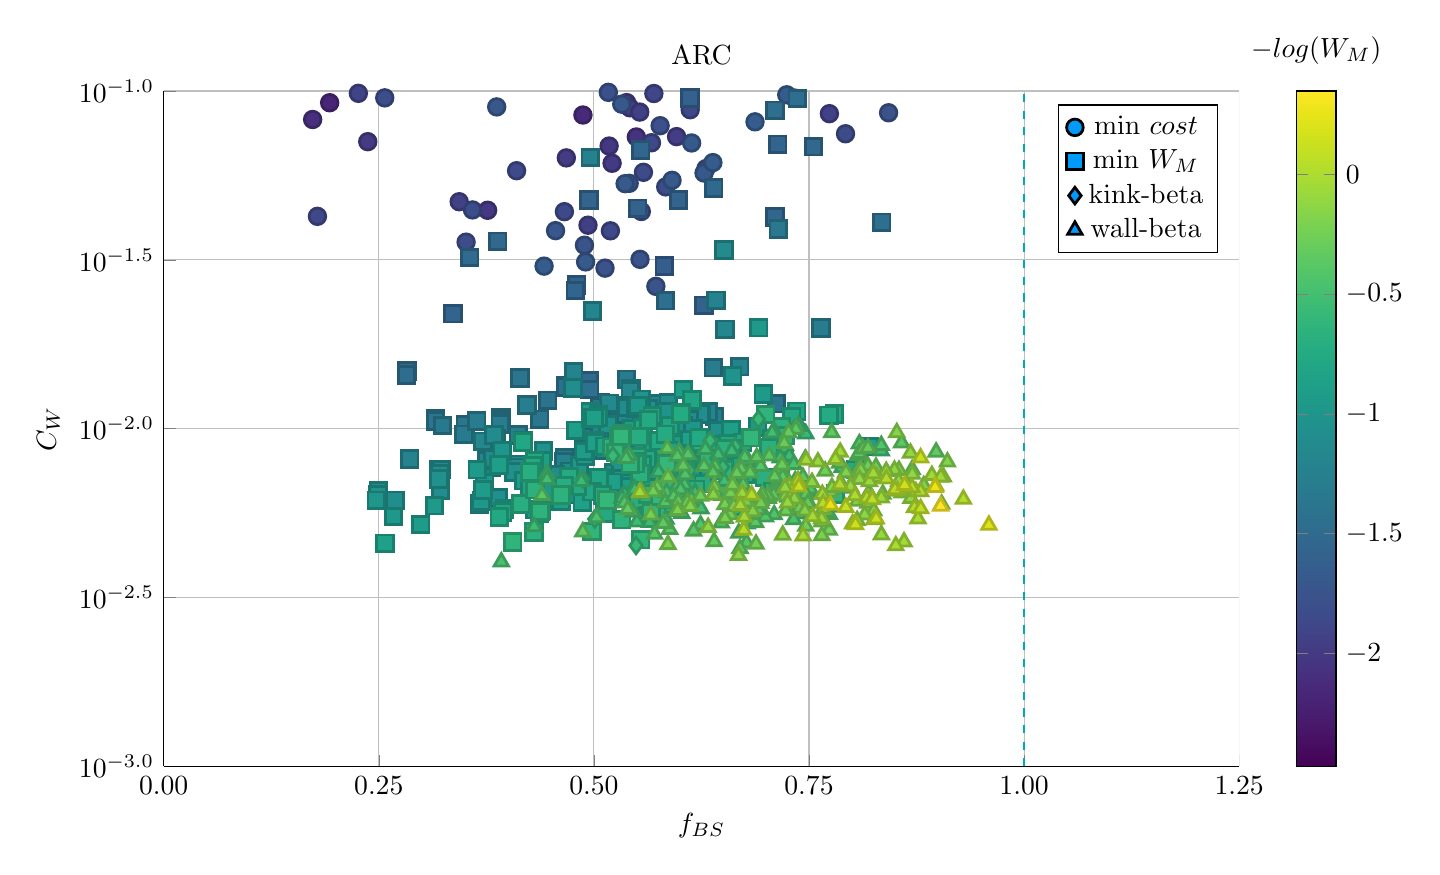
\begin{tikzpicture}[]
\begin{axis}[colorbar = {true}, height = {101.6mm}, ylabel = {${C}_{W}$}, title = {ARC}, xmin = {0.0}, xmax = {1.25}, ymax = {0.1}, ymode = {log}, xlabel = {${f}_{BS}$}, {unbounded coords=jump, scaled x ticks = false, xticklabel style={rotate = 0}, xmajorgrids = true, xtick = {0.0,0.25,0.5,0.75,1.0,1.25}, xticklabels = {0.00,0.25,0.50,0.75,1.00,1.25}, xtick align = inside, axis lines* = left, scaled y ticks = false, yticklabel style={rotate = 0}, log basis y=10, ymajorgrids = true, ytick = {0.001,0.0031622776601683794,0.01,0.03162277660168379,0.1}, yticklabels = {$10^{-3.0}$,$10^{-2.5}$,$10^{-2.0}$,$10^{-1.5}$,$10^{-1.0}$}, ytick align = inside, axis lines* = left,     xshift = 0.0mm,
    yshift = 0.0mm,
    axis background/.style={fill={rgb,1:red,1.00000000;green,1.00000000;blue,1.00000000}}
, colormap={plots}{rgb=(0.26700400,0.00487400,0.32941500), rgb=(0.27794100,0.05632400,0.38119100), rgb=(0.28291000,0.10539300,0.42690200), rgb=(0.28229000,0.14591200,0.46151000), rgb=(0.27619400,0.19007400,0.49300100), rgb=(0.26514500,0.23295600,0.51659900), rgb=(0.25042500,0.27429000,0.53310300), rgb=(0.23360300,0.31382800,0.54391400), rgb=(0.21813000,0.34743200,0.55003800), rgb=(0.20123900,0.38367000,0.55429400), rgb=(0.18555600,0.41857000,0.55675300), rgb=(0.17117600,0.45253000,0.55796500), rgb=(0.15772900,0.48593200,0.55801300), rgb=(0.14618000,0.51541300,0.55682300), rgb=(0.13374300,0.54853500,0.55354100), rgb=(0.12346300,0.58168700,0.54744500), rgb=(0.11948300,0.61481700,0.53769200), rgb=(0.12632600,0.64410700,0.52531100), rgb=(0.15014800,0.67663100,0.50658900), rgb=(0.19109000,0.70836600,0.48228400), rgb=(0.24607000,0.73891000,0.45202400), rgb=(0.31192500,0.76782200,0.41558600), rgb=(0.37777900,0.79178100,0.37793900), rgb=(0.45867400,0.81636300,0.32972700), rgb=(0.54552400,0.83803900,0.27562600), rgb=(0.63690200,0.85654200,0.21662000), rgb=(0.73088900,0.87191600,0.15602900), rgb=(0.81457600,0.88339300,0.11034700), rgb=(0.90631100,0.89485500,0.09812500), rgb=(0.99324800,0.90615700,0.14393600)}, colorbar style={title=$-log( W_M )$}}, ymin = {0.001}, width = {152.4mm}]\addplot+[scatter, scatter src=explicit, only marks = {true}, color = {rgb,1:red,0.00000000;green,0.60560316;blue,0.97868012},
draw opacity=1,
line width=0,
solid,mark = *,
mark size = 3.0,
mark options = {
    color = {rgb,1:red,0.00000000;green,0.00000000;blue,0.00000000}, draw opacity = 1.0,
    fill = {rgb,1:red,0.00000000;green,0.60560316;blue,0.97868012}, fill opacity = 1,
    line width = 1,
    rotate = 0,
    solid
}] coordinates {
(0.5241958664809654, 0.20287227770679064) [-2.471255345772589]
(0.6576174121055033, 0.2306439147061058) [-2.4448353783501813]
(0.5667366204542917, 0.21229572622839188) [-2.3420433442606363]
(0.5527453887086349, 0.17601810120802597) [-2.317452102945315]
(0.5061500178726741, 0.15646026161547585) [-2.271586680020917]
(0.2819526564955794, 0.23313397035671538) [-2.2454926622107947]
(0.5154131085826593, 0.30695982711321923) [-2.240477125239761]
(0.5121074780521085, 0.12981873154201856) [-2.221001617157497]
(0.36855232237120356, 0.20412561186382183) [-2.2185595731398573]
(0.4242321290991145, 0.17283887577812557) [-2.217742719332761]
(0.4047617309441989, 0.1723168352757067) [-2.1943652895954826]
(0.19286791326705938, 0.09228957678154598) [-2.180611452056678]
(0.5532714654641776, 0.18069474612421305) [-2.178533974810608]
(0.23145882806732, 0.17575721123179697) [-2.1613119546549586]
(0.564515028561278, 0.14737248164629663) [-2.153481889652779]
(0.2747981030966843, 0.15121971859178504) [-2.1532666027476224]
(0.4872417045079029, 0.08487876383400252) [-2.137355128792399]
(0.612166701787264, 0.18468615468864133) [-2.117721604472264]
(0.5023741300351264, 0.10225619683254578) [-2.112364994691398]
(0.17309553189891597, 0.08231272723595219) [-2.0932729799082814]
(0.8291596430779791, 0.18191471123359046) [-2.088330487139694]
(0.31718430150640886, 0.1065828154014555) [-2.0864754038765376]
(0.5273579873776012, 0.1272047508604084) [-2.0803726509713845]
(0.5595793743294597, 0.11257905190542687) [-2.0743439417542344]
(0.4605098153393489, 0.1600333280328488) [-2.060818046402037]
(0.5493219691145695, 0.07308016714475707) [-2.0557180072115067]
(0.31128212610729583, 0.12592715347430458) [-2.0556926961078257]
(0.37645603539027617, 0.044334788818868265) [-2.0190103037593397]
(0.5176809217159155, 0.06869458193202499) [-2.0160407406558845]
(0.7081188681434396, 0.1481536198793765) [-2.013932053549837]
(0.5211323398937894, 0.06108685421726483) [-2.00409352685897]
(0.5380552721473089, 0.09236557707945936) [-1.9956061889121497]
(0.23715847834480255, 0.07078434635359439) [-1.990719111417077]
(0.46795448687244745, 0.06336605700824453) [-1.9900844504935096]
(0.6557560817291185, 0.11627768440359171) [-1.9837616587056666]
(0.35068098774722584, 0.25526434794478386) [-1.9822717418460247]
(0.5960363570257688, 0.07325842242370716) [-1.9712120847707018]
(0.541926025336331, 0.08913847457348267) [-1.9636002811445543]
(0.7410857770713545, 0.15979638765383897) [-1.9571238190242108]
(0.3701358669693677, 0.20418232424592905) [-1.9546253727806209]
(0.5532971016447703, 0.08659458120814034) [-1.9463665380941702]
(0.4931141469968015, 0.040041103525576084) [-1.944009739142569]
(0.6750992151231566, 0.13342994620782112) [-1.9434041917067464]
(0.773711576159501, 0.08565629392349437) [-1.9426970317490913]
(0.34341778727051797, 0.04698977973717222) [-1.9371763921573384]
(0.40004180408095424, 0.11657734913990186) [-1.928537217281344]
(0.22621961396755902, 0.09839586000912476) [-1.9107205293107241]
(0.33982734439703416, 0.12275477488785659) [-1.9004071431399057]
(0.5696717164152757, 0.09825956480008603) [-1.8918218222163223]
(0.6089203094451604, 0.12138563536401357) [-1.8887149281050344]
(0.7855174188311217, 0.10048378866349675) [-1.8819056386780568]
(0.519165742162139, 0.03854677190172235) [-1.869430211714412]
(0.56689423388905, 0.07025107210769377) [-1.8651124798448722]
(0.17865306360793093, 0.04253804397177868) [-1.8644786123967394]
(0.6118904337598889, 0.08799392557650451) [-1.860496893823878]
(0.46571538383754973, 0.04391723622012491) [-1.8542903424441743]
(0.5575934736377758, 0.05743494936487108) [-1.8495112242429361]
(0.41012249247804866, 0.058061403117541356) [-1.846257438745883]
(0.7924354191473056, 0.07470510715125366) [-1.8416117842187498]
(0.5550986570410285, 0.04396908701659585) [-1.841317185146719]
(0.665840917415036, 0.14962201583537357) [-1.8309301799846331]
(0.6302313196317723, 0.05890018945608892) [-1.82730525270959]
(0.6638598475520857, 0.1158423978677618) [-1.826901690940231]
(0.2568814608902971, 0.09540606509282185) [-1.8239153211364227]
(0.6535189993672528, 0.12701003424511964) [-1.8168455226783244]
(0.3514379080061537, 0.03567637571358925) [-1.8166454759701696]
(0.35890190840174097, 0.0444388756442925) [-1.81017737836428]
(0.5834421319112952, 0.05199865811744338) [-1.8086978288671451]
(0.6467507601284886, 0.1251127775635393) [-1.798447628719369]
(0.7506773056708338, 0.14005152172406524) [-1.7969021740981885]
(0.5769610885682936, 0.0789099851468337) [-1.7945906278673165]
(0.5167473074126737, 0.09906247923337126) [-1.779933055929714]
(0.8424743258288371, 0.08619366633116249) [-1.7676381685595108]
(0.5128998814964993, 0.02988638548757804) [-1.7674346288089102]
(0.4890123747581225, 0.0349357030811516) [-1.748385793611066]
(0.5719886607137856, 0.026398091660566128) [-1.7474067398666728]
(0.5535801579795155, 0.0317308779482479) [-1.7473345345195481]
(0.6646042636427472, 0.13550842427034193) [-1.74675304289594]
(0.5410133779521771, 0.05327415376487706) [-1.7440444912963449]
(0.7331805458227827, 0.09528385676184899) [-1.7420641858951875]
(0.5323465099100665, 0.09137626462030565) [-1.7106233078102575]
(0.4554042355140383, 0.03859073092462427) [-1.7101957038204436]
(0.6280080521317699, 0.057157670859899604) [-1.6976377627866777]
(0.3870013471271922, 0.08970301543530995) [-1.6951046172778514]
(0.5908033630086555, 0.05437969052103555) [-1.6845366899487946]
(0.5362845083298821, 0.053158707255175616) [-1.6842882715798002]
(0.6135591627510759, 0.07015118809375721) [-1.6798255842338246]
(0.4903582554642052, 0.0311795818387021) [-1.678803886594569]
(0.7241153127543816, 0.09743173539150955) [-1.6644466872035906]
(0.44208173753609914, 0.03029149365815447) [-1.661845596221059]
(0.6382751599025954, 0.06136233850066078) [-1.6570891122908413]
(0.6872315803634489, 0.08102586935633366) [-1.6543345543312795]
};
\addlegendentry{min $cost$}
\addlegendentry{min $W_M$}
\addlegendentry{kink-beta}
\addlegendentry{wall-beta}
\addplot+[scatter, scatter src=explicit, only marks = {true}, color = {rgb,1:red,0.00000000;green,0.60560316;blue,0.97868012},
draw opacity=1,
line width=0,
solid,mark = square*,
mark size = 3.0,
mark options = {
    color = {rgb,1:red,0.00000000;green,0.00000000;blue,0.00000000}, draw opacity = 1.0,
    fill = {rgb,1:red,0.00000000;green,0.60560316;blue,0.97868012}, fill opacity = 1,
    line width = 1,
    rotate = 0,
    solid
}] coordinates {
(0.5817114877806479, 0.03030964076750237) [-1.6347176951799236]
(0.6118616823524671, 0.09519865042001042) [-1.6073278771107937]
(0.550825513446965, 0.04494796053659054) [-1.584364281605552]
(0.47990293428614395, 0.026650965215041525) [-1.5820971810203286]
(0.6280353944665124, 0.023183384776903366) [-1.581333652067033]
(0.49437603226420324, 0.047519264379099695) [-1.5776358054595747]
(0.3362571361359799, 0.021900164864569343) [-1.5739276291567563]
(0.5982172603264796, 0.04756226129621259) [-1.572108505738868]
(0.7135274551952335, 0.06954867549545035) [-1.5672962391673115]
(0.47833927674197335, 0.02566305684475041) [-1.5665040064849882]
(0.7103341191962936, 0.04235079729891905) [-1.5555149127719143]
(0.5543093285365798, 0.06695317015759708) [-1.543581310599075]
(0.7551306424351277, 0.06841478633789891) [-1.5260699424888133]
(0.3881783683118415, 0.03590196542626109) [-1.524227611937092]
(0.6393151095771953, 0.05163649629310236) [-1.5216893138751995]
(0.355597836411217, 0.032143280375917176) [-1.5039859914912947]
(0.4945318173106939, 0.013866958448834382) [-1.493326092363065]
(0.28281884884932085, 0.014801741304267257) [-1.487901247382047]
(0.28211632020593413, 0.014412667219330384) [-1.4777729839057352]
(0.7104365991482212, 0.08761412553231249) [-1.4621624345903141]
(0.7363692362152062, 0.09498385047870876) [-1.4604586034356677]
(0.8344486043341511, 0.04081913693413996) [-1.4587214825346047]
(0.46708133454393946, 0.01340972738128021) [-1.4490727286546803]
(0.5831555839731757, 0.023945948554713548) [-1.4457290774204032]
(0.5075718306406568, 0.011911642809951824) [-1.4426440160762033]
(0.46706461267458904, 0.013297745600298047) [-1.4402960124898458]
(0.4950737862291223, 0.013059974842794808) [-1.4297123303293562]
(0.5067238822314855, 0.0116292993719446) [-1.4185999884517813]
(0.44619912372103193, 0.012144168284609194) [-1.4088672496121717]
(0.31605802663087745, 0.010680636478422217) [-1.3865730777653493]
(0.41428673202754596, 0.0141353915084305) [-1.3853300727274243]
(0.712239885615206, 0.011858386666639936) [-1.3837167890494473]
(0.350431541268587, 0.01028527278110118) [-1.3831077459191452]
(0.43685814056517275, 0.010657247043679216) [-1.3769740136231394]
(0.3159315431374323, 0.010544710114440428) [-1.3745163187278553]
(0.5413118800861578, 0.01102120660236595) [-1.3615967553395791]
(0.7142435030748111, 0.039062963614451315) [-1.3533380016716623]
(0.3240459840226499, 0.010216036443098337) [-1.3372087645633441]
(0.3920447348241641, 0.010766373691067175) [-1.3345129020147544]
(0.6388083334581369, 0.01515074267205838) [-1.3192755308000974]
(0.39164878205902165, 0.010549186267561154) [-1.314224057600752]
(0.3488127094714696, 0.009622849310238562) [-1.3119655997760449]
(0.5378910611821822, 0.014012905880008366) [-1.3067859154211212]
(0.7641042278711495, 0.01987362470678978) [-1.306488109771051]
(0.36380256670479283, 0.010543596556449621) [-1.300448172019359]
(0.42213038169068423, 0.011753733588622684) [-1.2909613135050368]
(0.39123076658058537, 0.01032210691217398) [-1.290941195447848]
(0.412247493693321, 0.009573931433783737) [-1.288382478225186]
(0.4659585061159808, 0.008214078605189646) [-1.2848508011023854]
(0.38667992917631405, 0.009313214534419275) [-1.2663273942574376]
(0.6399920560778708, 0.010859939566305288) [-1.2628532071739471]
(0.4932184016134092, 0.00942852126782232) [-1.2571675985941009]
(0.4646455314624805, 0.007979384853642458) [-1.2548029920250783]
(0.3808496705423307, 0.007684943962399527) [-1.2437033135541056]
(0.4958659013831641, 0.06352567671838111) [-1.2369052187227225]
(0.5000213263897932, 0.009002465988456979) [-1.2270518720108157]
(0.5308438797997663, 0.011035208951789109) [-1.226245033465833]
(0.6694205694501582, 0.015249972586931702) [-1.2235700920501882]
(0.5693740544983247, 0.00868692401548569) [-1.2226473193604595]
(0.6417688448023928, 0.023992084814044464) [-1.2216425458700924]
(0.5487244266906349, 0.008820048824892238) [-1.2211984240451863]
(0.2858601406466925, 0.008128091853447697) [-1.2182589804749475]
(0.5156304286810139, 0.009127494309245325) [-1.2142161347607898]
(0.47639998325402977, 0.014715113037040341) [-1.2132136425529505]
(0.5288813993673583, 0.010793413620685892) [-1.206641818571807]
(0.5402250120741555, 0.009362601672990878) [-1.191936852103939]
(0.5727465096226879, 0.008532248708843341) [-1.1915692690246116]
(0.4984364208598661, 0.022329699785653967) [-1.1862171477514327]
(0.6327644843335064, 0.011220902449602043) [-1.1850949532660688]
(0.5065941888585173, 0.009964976977277301) [-1.1849042685186388]
(0.3751135189163956, 0.008046818607636182) [-1.1783816195421168]
(0.5288430725634312, 0.010502630239530353) [-1.1745570808178625]
(0.5743220494611327, 0.011831696332363917) [-1.1739049960816583]
(0.49014706797846697, 0.008338714638816998) [-1.1727262972250005]
(0.5428976258536967, 0.013100649505701023) [-1.1685715861060364]
(0.4876473654064088, 0.008679297866717622) [-1.1678361124508785]
(0.37098217471657124, 0.009176059619375874) [-1.1638475083020863]
(0.6512553694339193, 0.009147667338886346) [-1.163646396682439]
(0.5119225508554565, 0.008821522947817238) [-1.1625884970295683]
(0.6522013945133583, 0.01969269746480885) [-1.161263163747147]
(0.5367974717464423, 0.011052820822833412) [-1.1612436952445022]
(0.5422654663131025, 0.012951176392377263) [-1.1564975464369418]
(0.5110846173942302, 0.00865659180620948) [-1.1564777605259131]
(0.5353295518280365, 0.008539920889371473) [-1.153669555256764]
(0.5173196862178037, 0.011881223263670228) [-1.1449033146577834]
(0.6129510277633284, 0.011182674502441104) [-1.1446379399297224]
(0.3201525037042981, 0.00758528934201417) [-1.1369019245716605]
(0.642193788855941, 0.009173443590563553) [-1.1296752949778874]
(0.5535992683176709, 0.008338540154559412) [-1.1286199217371102]
(0.6513872112772378, 0.03379772419568562) [-1.1227901581286868]
(0.5384174946071185, 0.011716658365690755) [-1.1213706798498402]
(0.44262055397654837, 0.006600498288231924) [-1.120744758255219]
(0.38214281120318244, 0.008128082189126142) [-1.1202374603300567]
(0.4722194839752176, 0.007485071081146149) [-1.1198130519550673]
(0.3228255089630173, 0.00757188435534942) [-1.1197010006946204]
(0.38371417796295587, 0.0095811845612121) [-1.1171509659015317]
(0.624252275623572, 0.011241415941032132) [-1.1142292859317902]
(0.5355455264892967, 0.009608134033428447) [-1.111737343141002]
(0.5727668427351763, 0.01112408759755598) [-1.109744376511266]
(0.4114801256653036, 0.007847073705149175) [-1.1077966249084845]
(0.5382787031018355, 0.011559534016906275) [-1.1071823666105103]
(0.31965994829173516, 0.0073510161641234155) [-1.104798498774279]
(0.5384075099986052, 0.007531141843880735) [-1.1010716645822378]
(0.5864126224331899, 0.011959627018568285) [-1.1002751733513731]
(0.557617660880907, 0.007903291194171595) [-1.100001261719793]
(0.47549886995354823, 0.013186084887405795) [-1.0994225265487236]
(0.623037942078233, 0.011066567940261007) [-1.0985618635225085]
(0.5033268621050487, 0.00915283698682942) [-1.0949280603220852]
(0.2688518460791765, 0.006133703525212153) [-1.0934361516365225]
(0.6110478224857046, 0.010640115882783727) [-1.0929493330528903]
(0.558520760663903, 0.008947359142857395) [-1.0928608320296447]
(0.32155511158393607, 0.0073486051811523) [-1.087706069497112]
(0.4758264456361486, 0.006376305301764062) [-1.0862007240731857]
(0.4097926766511398, 0.007683528007593692) [-1.0852670263146056]
(0.5502315352756275, 0.008000466946774797) [-1.0851636190972072]
(0.5566953268770855, 0.0076693437218355535) [-1.0840894132396022]
(0.3216722475930553, 0.006579330015555362) [-1.0835229356564555]
(0.45567205862575944, 0.007297986251593657) [-1.082817350704825]
(0.36696671117349405, 0.005986051223044731) [-1.0820717451803519]
(0.3891852359575543, 0.006234773177915995) [-1.072577404791479]
(0.24971176414080096, 0.00656095951928795) [-1.0722121269518887]
(0.5633918208276852, 0.011424148754591202) [-1.0713713808748146]
(0.6042975616419993, 0.01019215515273024) [-1.0693614816162402]
(0.5485022627546088, 0.011520946380794598) [-1.0668579057002654]
(0.5553825174671281, 0.008690353228069395) [-1.0614717160120588]
(0.6436681416631705, 0.009857214240237989) [-1.0539224257593203]
(0.5231064369976265, 0.007410533138876833) [-1.0510937327305279]
(0.4070604216031404, 0.007449838707835127) [-1.0497007973704187]
(0.3198885646073333, 0.007088919319303044) [-1.0471558619826447]
(0.4414420283273741, 0.008599918404779687) [-1.0461189694088024]
(0.24867057556472014, 0.006377309887140109) [-1.0418966319978196]
(0.6376541673006868, 0.0075647796759351965) [-1.038421761130219]
(0.6009251138878389, 0.009882058577592544) [-1.036521934372695]
(0.41776764665149635, 0.009223959289867847) [-1.0356215569640665]
(0.5842492103852158, 0.011206142984745959) [-1.032265172493932]
(0.5159535753171318, 0.010275809470086928) [-1.0209529420786516]
(0.4959672719731226, 0.006909070463416791) [-1.017778295850808]
(0.661391258299459, 0.014318337912922812) [-1.0164185835880817]
(0.5608498014090172, 0.010831709750721097) [-1.0158514857486804]
(0.6151725048676855, 0.009969004456469335) [-1.0092640911327964]
(0.5314443614911326, 0.0076830709125841655) [-1.0065489183190215]
(0.5286944439645233, 0.007109903886026088) [-1.0049567352420634]
(0.5552755893210628, 0.012210250424143995) [-1.0009019288888164]
(0.5581675745958038, 0.007769954338030814) [-1.0006461053349212]
(0.24716026898994242, 0.00614165224338566) [-0.9994054785850832]
(0.504350487641437, 0.006788464214574843) [-0.9973161692403991]
(0.3934424737113256, 0.008588102458327246) [-0.9969035241117329]
(0.4796243766218075, 0.006868288351132624) [-0.9965363238277729]
(0.52700034066082, 0.0068423979356222785) [-0.9922669644795622]
(0.37317354020546645, 0.006930487452016415) [-0.9885003181225582]
(0.6089875710029672, 0.008132058870519111) [-0.9840022040037167]
(0.4213909625587017, 0.007028212307439231) [-0.9804048117014232]
(0.4833180602931159, 0.007774353597955766) [-0.979522354913071]
(0.26710604767533075, 0.0054956368744154315) [-0.9765348801577157]
(0.42944101394074274, 0.007267240459298835) [-0.9755629318997818]
(0.3691943435583234, 0.0061040685529331245) [-0.9749892927335156]
(0.49008340947678686, 0.008312108043668191) [-0.9674264957309127]
(0.43100817708896116, 0.005754155204131383) [-0.966984586559087]
(0.3146511741196146, 0.005916229247218672) [-0.963620689023264]
(0.6915196643186565, 0.019907252097557806) [-0.9635570646594878]
(0.6969186730398873, 0.012656834856123324) [-0.9589381201418358]
(0.5343246872696013, 0.006890734339357853) [-0.9584027445972434]
(0.5516547055046426, 0.01170966388492377) [-0.9563855192144691]
(0.45055913702267586, 0.00648495859205545) [-0.9554467273670927]
(0.36443125720312075, 0.0075610875798886755) [-0.9545632580533228]
(0.6903219512667356, 0.010114178702367332) [-0.9528002583069045]
(0.592139488874089, 0.009004872969664781) [-0.9496533928753537]
(0.49580893715304947, 0.011207230671626593) [-0.9413852860902241]
(0.6235670164997241, 0.007146213704940033) [-0.9370119952675158]
(0.37108589969685146, 0.006581879826789411) [-0.9331828097449962]
(0.6437665262857747, 0.008767448947945771) [-0.9329352040317512]
(0.4888947150611439, 0.008557021700551098) [-0.9324303568969876]
(0.2986086480277226, 0.005203512160232155) [-0.9311662336138826]
(0.6255293508491894, 0.008081114013096696) [-0.9287944685604638]
(0.6140870094258984, 0.007628598443188674) [-0.926890870969113]
(0.41876798527701836, 0.007018485606889323) [-0.92386498939783]
(0.5054852519528996, 0.011015711855547592) [-0.919580931517054]
(0.4786536293159207, 0.009893013391436023) [-0.9180169825194476]
(0.5441671870525477, 0.009982337828276887) [-0.9154453649397588]
(0.5007878466101845, 0.0091944581117192) [-0.9139490923741643]
(0.561487282467392, 0.007833072636536566) [-0.9132133538239265]
(0.6514919308345418, 0.008840033410607953) [-0.9121378643433682]
(0.6039078741957786, 0.013068265001934793) [-0.9110784645494641]
(0.6227409498560608, 0.007938450262022891) [-0.9098658111730449]
(0.6435481039076728, 0.008553630272950136) [-0.9070051498915257]
(0.6010749539644062, 0.007575552407024117) [-0.9067782074518957]
(0.5348620647926116, 0.006729621026089755) [-0.9060762300599821]
(0.8195604933647264, 0.008858181214516578) [-0.9039670080592699]
(0.4960911849247666, 0.010768315647388733) [-0.9014867608639769]
(0.5049187404089968, 0.010808877533630424) [-0.9007952929826429]
(0.5008305537160933, 0.009078214918907012) [-0.9007062506970809]
(0.5137960656889574, 0.007073305102824147) [-0.900208401387847]
(0.4299758063065358, 0.007716380916945232) [-0.8984405159461796]
(0.461950405654823, 0.006106767180219444) [-0.8982477432771846]
(0.6509355541893169, 0.008695264992095957) [-0.896003666359785]
(0.5225903676252684, 0.006941829479120447) [-0.8955056224321819]
(0.3894845570414093, 0.007814299518066377) [-0.8942100046557695]
(0.4394904947732839, 0.008028972189491295) [-0.8890699913254794]
(0.5003005570537615, 0.010728044838137048) [-0.8876712498055658]
(0.5845386590677969, 0.008310610689471132) [-0.8863260728535448]
(0.6591714169241578, 0.00991040208694835) [-0.8837201982810288]
(0.5754886167651249, 0.00719216253641406) [-0.8834009298105716]
(0.42859653650833, 0.007585939375582381) [-0.8806916777259077]
(0.6118081005357805, 0.009272863725182066) [-0.8796719383127752]
(0.48641611954822667, 0.006055492371240138) [-0.8726396490009896]
(0.257229546671479, 0.004580349740413994) [-0.8672923383997936]
(0.426462607268772, 0.007407120757886044) [-0.8535433362712267]
(0.5686669963907276, 0.008621646255895433) [-0.8533325571574846]
(0.6175106036050393, 0.006609354191499301) [-0.853129954975184]
(0.5877104639523651, 0.008626640245331227) [-0.8458427202328871]
(0.5716419045548307, 0.007926356626055567) [-0.8399949391566971]
(0.3962776710982887, 0.005783758781719592) [-0.8344337866440044]
(0.4255334400440256, 0.006679285642911387) [-0.8328143677232719]
(0.43857941286956165, 0.005735056256784172) [-0.8320308752066863]
(0.5769445652964436, 0.007843029441706253) [-0.8221569652352421]
(0.6611817268556156, 0.008093343165007398) [-0.8172218943340012]
(0.5126668648272711, 0.008863355456490663) [-0.8131136245599477]
(0.3941080030492619, 0.005668771371327368) [-0.8122740065328773]
(0.506119518337849, 0.007155161987838886) [-0.8080036926936133]
(0.6141107199137688, 0.008031459191263671) [-0.8071539542338575]
(0.6139955223319464, 0.012167930923139617) [-0.8069124707651293]
(0.6417146223223801, 0.008948962637139601) [-0.8052829756994823]
(0.5669733040046213, 0.006679423174117699) [-0.8020427686638395]
(0.7356948340040768, 0.011264900432107284) [-0.8005903298305235]
(0.5882544255345495, 0.0101736730249019) [-0.7977331662395057]
(0.6728655549820258, 0.009118819889961022) [-0.7969461494732382]
(0.5679841220109311, 0.01094150991845671) [-0.7969287961306641]
(0.6222675762661165, 0.009204618947872185) [-0.7946481033628194]
(0.4310732454261373, 0.008047254921185912) [-0.7926515245490977]
(0.4177825334190035, 0.009132260578460593) [-0.7893816917258589]
(0.4369556767367021, 0.005606722466908005) [-0.7891633883074732]
(0.4977504961312478, 0.006506117273958602) [-0.7806626165140812]
(0.5618987698011563, 0.008151671842735457) [-0.7792790884221499]
(0.556998592933926, 0.010062331825114089) [-0.7784524078397926]
(0.6554923199603303, 0.009001558635684543) [-0.7779808320754125]
(0.39004777043616934, 0.0054810011900626385) [-0.7720609309973395]
(0.5562151504078756, 0.00782695612444411) [-0.7652054854871606]
(0.5635456677693395, 0.010602248839245204) [-0.7637174087569671]
(0.7298248277431699, 0.010869712908743537) [-0.763435051327913]
(0.5099920259552589, 0.006363325083353543) [-0.7618517639809802]
(0.7795217235236127, 0.01105835991924475) [-0.7614993450910051]
(0.5128038581202035, 0.005635574040670621) [-0.7611032574956281]
(0.5843531099526409, 0.007945573763413242) [-0.7586493247490348]
(0.6783775994948534, 0.00746361599356464) [-0.7555286255013439]
(0.4287240355308217, 0.0077689317654998065) [-0.7546589867802752]
(0.615129822924657, 0.008443992254390653) [-0.7545235423813055]
(0.6198452199457032, 0.008351019459044646) [-0.7530552699688687]
(0.575573732558629, 0.009207860738462068) [-0.7525689023877592]
(0.6510139446420534, 0.0076258608035912135) [-0.750871938891472]
(0.6224512800040214, 0.009388924409384974) [-0.750814319098593]
(0.6012103864677005, 0.01118644198035734) [-0.748723305421913]
(0.7069020464705562, 0.009345849525045828) [-0.7483206071488305]
(0.4805514422966483, 0.006768249757897973) [-0.7464367414626797]
(0.4708373767438117, 0.007223518482823314) [-0.7461140334995429]
(0.7731485889984414, 0.010949849394014196) [-0.7445921563372909]
(0.8037621486342045, 0.0075644226280255) [-0.7405170531585982]
(0.6757344825134481, 0.007343719666417131) [-0.7390004613202035]
(0.6594328314470048, 0.008700856720017821) [-0.7387616236204831]
(0.626762429902987, 0.00688316527472499) [-0.7380863769707697]
(0.5829650043598863, 0.00962175642804203) [-0.7368937154713704]
(0.6007965815988566, 0.011034885333216478) [-0.7342730225098203]
(0.5580883743814108, 0.006379564580150208) [-0.733902575813519]
(0.5441864591828873, 0.005838014810087431) [-0.733366320896288]
(0.570430479648329, 0.005798113597019041) [-0.7194953671868318]
(0.4653459017068548, 0.006758912533271294) [-0.7147746128167595]
(0.5523041252103958, 0.009475051889139297) [-0.7131077088888362]
(0.41526223236330206, 0.005978841286873692) [-0.7060108538400767]
(0.42552016721166286, 0.007437940638478416) [-0.7054470522681139]
(0.6239617621329132, 0.008396523209957296) [-0.7043302537280044]
(0.6279845069667198, 0.008135075629052014) [-0.7004921579289034]
(0.5881492261240776, 0.006868958471786255) [-0.7001780528099326]
(0.5506350458775752, 0.00825632250348302) [-0.6977184423457128]
(0.6979968249478757, 0.007177220657115959) [-0.6956779138722414]
(0.6568303568061684, 0.007022224715140027) [-0.6951251649106842]
(0.6182818991073687, 0.006613282053180216) [-0.6924358169248216]
(0.5510239579883293, 0.0061493207913365135) [-0.6909665152137748]
(0.5702234268112552, 0.006107066134008809) [-0.6835279600057703]
(0.703320903908008, 0.008780796565424387) [-0.6827611083117922]
(0.7077673334600145, 0.0065261506973616846) [-0.6795072230761997]
(0.5495829548416775, 0.00800959338461906) [-0.677700463862544]
(0.4314935730470368, 0.006600686007871915) [-0.6763055623723756]
(0.43054195576046844, 0.004950028138324652) [-0.6703030174757271]
(0.5635130294426022, 0.005539486392576543) [-0.6677810778235018]
(0.553595959152619, 0.007362527200082348) [-0.6673391087292244]
(0.6519599706166325, 0.008739904111948478) [-0.6667743364683484]
(0.5824517878555476, 0.006646109301375384) [-0.6628604680937062]
(0.7176408995573551, 0.010112687007456347) [-0.6619264755699156]
(0.5770682825422682, 0.005808955328171345) [-0.6609430387636127]
(0.6024550183113115, 0.006226486976685874) [-0.6608237273970524]
(0.5478348614019433, 0.007880168654276763) [-0.6591974827031457]
(0.5208453986930105, 0.00880835203629707) [-0.6555251605106848]
(0.5959294410528901, 0.0069051641790013815) [-0.6502439759277362]
(0.46157053437184653, 0.006370154893781598) [-0.6501176336530103]
(0.716721708615555, 0.007046016170190783) [-0.6471624229162491]
(0.5422497797368149, 0.00786400613866977) [-0.642689222490187]
(0.676581400539928, 0.006126476505793275) [-0.6426719680934136]
(0.43755139645655033, 0.00568605172293329) [-0.6421657799692642]
(0.5322226344638359, 0.005380439014465079) [-0.6408278053086536]
(0.6315922459562998, 0.008151332535041496) [-0.6390518480231551]
(0.5289646632563154, 0.009445426881617458) [-0.637387036100165]
(0.5629402113776424, 0.006410449458406456) [-0.6331856765913819]
(0.6064256092688981, 0.007534711658278645) [-0.6317878364268024]
(0.699534914937192, 0.011020608245919671) [-0.6302067113060754]
(0.7227329826277413, 0.009531906181488446) [-0.6300141158962402]
(0.5326012265639793, 0.009634058044917598) [-0.6280804941242557]
(0.6330084093380534, 0.008014239654104959) [-0.6280494211696446]
(0.6507439971206197, 0.007547331772442004) [-0.6280078234260247]
(0.40558390299155495, 0.004613850780468482) [-0.6272747005855834]
(0.7806276684554971, 0.006403443257132637) [-0.6249924315441349]
(0.5542724771727453, 0.004688384323580258) [-0.6203497363094942]
(0.7379632139747722, 0.00673286293260975) [-0.6186335699037506]
(0.6491547712439395, 0.006536718541121758) [-0.616611980354735]
(0.4976979810985317, 0.004961181636973083) [-0.6158983852690758]
(0.5922925103137072, 0.005978684032577509) [-0.6126591649688387]
(0.6603227030387234, 0.005906726926903094) [-0.6115944493416251]
(0.5316308102551144, 0.00947881794063107) [-0.610433329147383]
(0.6827036729203786, 0.009411403397962845) [-0.6100633867421124]
(0.587302343499971, 0.006804926481153247) [-0.6086993044360022]
(0.576987349595759, 0.006194075724438983) [-0.5997038129358795]
(0.5849100380517773, 0.007840734610599833) [-0.5989923200136442]
(0.5667143656682501, 0.005628681372057809) [-0.596937261397637]
(0.525146575549925, 0.008492276760383373) [-0.5958587738741902]
(0.515389531675495, 0.006157094838169622) [-0.5927256123541282]
};
\addlegendentry{min $cost$}
\addlegendentry{min $W_M$}
\addlegendentry{kink-beta}
\addlegendentry{wall-beta}
\addplot+[scatter, scatter src=explicit, only marks = {true}, color = {rgb,1:red,0.00000000;green,0.60560316;blue,0.97868012},
draw opacity=1,
line width=0,
solid,mark = diamond*,
mark size = 3.0,
mark options = {
    color = {rgb,1:red,0.00000000;green,0.00000000;blue,0.00000000}, draw opacity = 1.0,
    fill = {rgb,1:red,0.00000000;green,0.60560316;blue,0.97868012}, fill opacity = 1,
    line width = 1,
    rotate = 0,
    solid
}] coordinates {
(0.6426659794233436, 0.00815561907827368) [-0.5919909182692854]
(0.5467348022827744, 0.006659517069337427) [-0.5900649293210665]
(0.7190311064983813, 0.007508093393788605) [-0.5846116951906657]
(0.6111339025872151, 0.007527132152211165) [-0.5833148125881625]
(0.6497883761170222, 0.007696247444472184) [-0.5830287350896988]
(0.6912674151371413, 0.010658010749014063) [-0.5820887710705529]
(0.5010169539514072, 0.005401882204713616) [-0.5820189989610497]
(0.535207082269819, 0.006378967305214437) [-0.5810074819933287]
(0.738016225952711, 0.010217682877138867) [-0.580249699669254]
(0.6642282356732003, 0.008850762543020996) [-0.5794750614001255]
(0.7241697567719548, 0.008618003799358996) [-0.5792296887118283]
(0.6755643086904745, 0.007360374433648833) [-0.5788547078152965]
(0.5490007479996606, 0.004512048645314757) [-0.57645307994183]
(0.7689819041990633, 0.006116989896278519) [-0.5763924759645073]
(0.5220335653648919, 0.008318627601371252) [-0.5729750222272765]
(0.4868290703396239, 0.007101945083232647) [-0.571357101904463]
(0.8201613481545499, 0.0074318775027898635) [-0.5687383147863687]
(0.6349821386738914, 0.00921889738378825) [-0.5664495516615029]
};
\addlegendentry{min $cost$}
\addlegendentry{min $W_M$}
\addlegendentry{kink-beta}
\addlegendentry{wall-beta}
\addplot+[scatter, scatter src=explicit, only marks = {true}, color = {rgb,1:red,0.00000000;green,0.60560316;blue,0.97868012},
draw opacity=1,
line width=0,
solid,mark = triangle*,
mark size = 3.0,
mark options = {
    color = {rgb,1:red,0.00000000;green,0.00000000;blue,0.00000000}, draw opacity = 1.0,
    fill = {rgb,1:red,0.00000000;green,0.60560316;blue,0.97868012}, fill opacity = 1,
    line width = 1,
    rotate = 0,
    solid
}] coordinates {
(0.7462328069126333, 0.009658524804105862) [-0.5601806209906858]
(0.733172140132461, 0.009987089667958969) [-0.5562142102431887]
(0.5325765388928654, 0.006226980540213371) [-0.5546880975085333]
(0.48540116680452616, 0.006988389031410877) [-0.5546446379212883]
(0.7213776765994893, 0.008732199148890674) [-0.5527698445398843]
(0.5646666533871787, 0.0052782873859023235) [-0.5511724233466424]
(0.6714883414104902, 0.006758297452000886) [-0.5458972121667514]
(0.6601590663603173, 0.008578141254814193) [-0.5458860807447207]
(0.61755852581437, 0.006467365285710576) [-0.5458790392173498]
(0.6069869283782695, 0.006443372817331658) [-0.5442175823270508]
(0.5750781331317051, 0.007444861036885179) [-0.5413629376616981]
(0.727120523648623, 0.008302826464105732) [-0.5407622305316014]
(0.8128499975149293, 0.007384818258648993) [-0.5380836133571618]
(0.4306345366490387, 0.0051300400638977835) [-0.5271444131838583]
(0.8339385882595673, 0.008602828358081035) [-0.5255090614858061]
(0.5500607622948984, 0.005298542813562824) [-0.5253112111160531]
(0.7164670912246649, 0.00819333918907477) [-0.5250086452090449]
(0.5474078932391263, 0.006599322440552919) [-0.5242581607842178]
(0.4452999137040005, 0.007353208884415579) [-0.5231634782341672]
(0.7094608911319944, 0.009826071077992524) [-0.5227222290441186]
(0.6704331503746649, 0.007775498450419187) [-0.5219300178618078]
(0.6444318946293824, 0.008375722675050382) [-0.5198234212377003]
(0.7146410804813309, 0.007439576027519643) [-0.5189423618344886]
(0.8072587227386677, 0.007085938022585789) [-0.5186559955617387]
(0.6515622757906024, 0.006989705805817807) [-0.5166768825560152]
(0.5836822932756094, 0.005403589710063612) [-0.5164750444191784]
(0.6780755069604057, 0.00522792590340526) [-0.5150980193064546]
(0.7071972425081949, 0.009714078296726672) [-0.5116011475894415]
(0.679146758206047, 0.008045443940040638) [-0.5108110236477874]
(0.6808115221769371, 0.006168650038348271) [-0.5086504350341889]
(0.7374570975653366, 0.010169283525689762) [-0.5058613464182684]
(0.8044487812948686, 0.007149224983922412) [-0.5044722675881411]
(0.6296116692519093, 0.008692377887529698) [-0.5031231924360503]
(0.44561234746837186, 0.007078098376377251) [-0.5028014569802962]
(0.7371135032871843, 0.005600084111327829) [-0.49869154414562766]
(0.6021442829696081, 0.0056125112484924035) [-0.4964599787823767]
(0.7378562224611037, 0.006989055802710069) [-0.4945330849408947]
(0.6013683340726933, 0.007748863368021302) [-0.49445009887788993]
(0.7119963782427297, 0.006902280893600737) [-0.49421586588303207]
(0.5455023731513893, 0.00566014678548545) [-0.4927895263450095]
(0.7255648759242043, 0.006279314886066035) [-0.49104432776578616]
(0.60544395537041, 0.0068196328329766425) [-0.4894491120094672]
(0.7255010248872851, 0.00586645675685587) [-0.4893731598482633]
(0.5961553356023347, 0.006713212862122576) [-0.48832643657065083]
(0.5405651809371826, 0.008344152391720813) [-0.4837586148470547]
(0.6244169439986023, 0.005795513687709428) [-0.4825057004434148]
(0.6699821798782176, 0.006822419925958226) [-0.4783695632105468]
(0.7884090567905805, 0.0076750515586257026) [-0.4778398107696417]
(0.7519821815458965, 0.006526727405836678) [-0.47615589494341126]
(0.606748467416823, 0.006076553561977724) [-0.4730246070917381]
(0.392373899848176, 0.004034790840437016) [-0.470381466184941]
(0.5844565869358972, 0.006479697957912273) [-0.46993988320225344]
(0.5374613782498835, 0.008165717336542033) [-0.4599766548042699]
(0.7321744577656044, 0.00538496287190979) [-0.45679107520810514]
(0.7323003853039213, 0.007848284231912143) [-0.4556219511821275]
(0.6005621660529309, 0.006600712155717754) [-0.4541668738184995]
(0.5031187110819957, 0.005454374636268768) [-0.4541064555241812]
(0.6126170800310774, 0.006125431816143641) [-0.4482955765676848]
(0.668355629932245, 0.0049059331399938155) [-0.44330924134877586]
(0.5946405329652326, 0.0056884836810024665) [-0.4427268704486458]
(0.606127810669948, 0.00731015290010166) [-0.44041188876301346]
(0.5990118160542135, 0.008551905531982902) [-0.4365732513919964]
(0.7456229467861399, 0.006367061568570841) [-0.43442596765666475]
(0.7202208309321447, 0.006761746354812581) [-0.43387758013866323]
(0.70952783567679, 0.005563916117757399) [-0.4286538673039319]
(0.699400290911475, 0.005480365884552941) [-0.4276593825982841]
(0.7393643087306998, 0.0062328465646338095) [-0.42677922558914155]
(0.6754629940735157, 0.00823395238579714) [-0.4265845359620904]
(0.7735702723950867, 0.005576683303865097) [-0.4263068075286862]
(0.6409170657777765, 0.007743741682150177) [-0.4248706605294772]
(0.5355224195610914, 0.0060366402560654946) [-0.42413966208895976]
(0.6479845635204572, 0.005263353300940577) [-0.4238953032901039]
(0.8085801490222563, 0.009024229969660702) [-0.4219301249136499]
(0.7118120504162843, 0.006671380181833438) [-0.4212383781626998]
(0.6595230555223146, 0.006486848222760267) [-0.4211778292210473]
(0.7756989961427158, 0.005863656687390416) [-0.42083484997410747]
(0.6239423318389465, 0.0051872913966039755) [-0.4176858743982254]
(0.8340073111971985, 0.008923153267776813) [-0.4125562162366198]
(0.751253706001916, 0.006633187100771731) [-0.41169860837029726]
(0.6131944579781969, 0.006189362812918045) [-0.4099354279936363]
(0.6093952446214297, 0.0083818741421803) [-0.4085744725915447]
(0.5826706652528132, 0.006049286496410891) [-0.4069630403485362]
(0.5968306925560191, 0.008297436412824197) [-0.4049846840705445]
(0.6937388488296713, 0.007742960768709124) [-0.4042004215441917]
(0.807827302186393, 0.007710669480181297) [-0.40320375837586364]
(0.7493153652493619, 0.006046061667925805) [-0.4028688677214397]
(0.5704013306287763, 0.004876529539216102) [-0.40001632289493805]
(0.5926248386168477, 0.006291433392085979) [-0.39976440163800875]
(0.7457396490099157, 0.008125237867570167) [-0.39804950655742244]
(0.6735584244562056, 0.006832906261032673) [-0.3970770857727276]
(0.7113953447902368, 0.006432248216156749) [-0.3908177018779014]
(0.7339871047747247, 0.007013862412780068) [-0.38805955987639323]
(0.7898500761552186, 0.006674804159855323) [-0.3864584691344222]
(0.6415707821544318, 0.006515832091950333) [-0.38429551664195744]
(0.6773994051537632, 0.004594344989791947) [-0.38405297410594313]
(0.6909900491216344, 0.005763218077573875) [-0.3831646466050567]
(0.6878883276184834, 0.005276300390961798) [-0.38294236861775216]
(0.7696564625783999, 0.005655464618579456) [-0.38288131062137803]
(0.43972942177297236, 0.006343046844021776) [-0.3823751133382093]
(0.6279411180967263, 0.00773200722515927) [-0.38146928666653984]
(0.8066328176721882, 0.008319222350851295) [-0.3795965309572695]
(0.5880353468087063, 0.005035636185664139) [-0.3740567262619664]
(0.6384363974416298, 0.0074073940583266225) [-0.37299740292253786]
(0.7464667473070459, 0.006389790707824904) [-0.3718977586029718]
(0.6158214440985598, 0.004979442746730671) [-0.3704439735448674]
(0.7214914188453198, 0.007296148641962362) [-0.3699388031456463]
(0.7088888557638892, 0.0065537429344493196) [-0.3673465484223324]
(0.7088839124292632, 0.006366328648950684) [-0.3663620347324109]
(0.554740742245829, 0.0065777201335919366) [-0.36473337871738076]
(0.7036680845446371, 0.008314725163938977) [-0.3621711889526386]
(0.8081121115464637, 0.008453236325245295) [-0.3621650615964567]
(0.7347906764983646, 0.009973310900945706) [-0.36211407373184695]
(0.785627176052173, 0.007908310098930752) [-0.358208177595687]
(0.85769284659742, 0.009085903374204375) [-0.3540595481577626]
(0.7292127935645752, 0.006346372007983234) [-0.353783118987174]
(0.7025239274779016, 0.0062192322127949005) [-0.35222463984026725]
(0.6904176389091119, 0.006037846604665242) [-0.3509025316268699]
(0.68923863079158, 0.008219213212955191) [-0.3505156401151719]
(0.7194618784241424, 0.0071884275030477075) [-0.34878832738313265]
(0.5556996388457375, 0.00640473519456716) [-0.3487293927724059]
(0.5806449815867873, 0.005242566183300256) [-0.3486265306507511]
(0.487101447577098, 0.004953286831218666) [-0.34709862801790886]
(0.6788253617118697, 0.005579652995774056) [-0.34579538401191395]
(0.6712687791027109, 0.007605183233966239) [-0.3424563617974656]
(0.5852531196610041, 0.008735028669940696) [-0.3416033910693547]
(0.6037941347834902, 0.007765678335692214) [-0.34067853168746914]
(0.669849925543272, 0.0044186510908645555) [-0.3399736780843229]
(0.5981621229953624, 0.00608996017461546) [-0.338097158267768]
(0.7764273811030159, 0.009734075214323398) [-0.3365189504472298]
(0.7429306227701317, 0.007182100285560063) [-0.3342891730139759]
(0.6814458296939387, 0.007395805129436751) [-0.33167488909851983]
(0.5393204677113422, 0.005770841448209159) [-0.3291558439371231]
(0.8977658080716024, 0.008531080054659001) [-0.3288043116425627]
(0.7023598722922598, 0.006310173960896718) [-0.32476450154274666]
(0.710081245288327, 0.007214539121290076) [-0.32435318438981625]
(0.8127952118927109, 0.008710866915913636) [-0.319394408736133]
(0.7262796040046966, 0.009745344842135342) [-0.318059813885549]
(0.7486340841195007, 0.006011707372419077) [-0.315839426619473]
(0.6660543607455871, 0.007379264780228708) [-0.3097939012350434]
(0.639724902525852, 0.004628681860959736) [-0.3065933727635902]
(0.5736264569495717, 0.006703155347445825) [-0.30207724924682977]
(0.701807469828968, 0.006303028558376165) [-0.2998550211328211]
(0.6956810800924564, 0.006372591850870413) [-0.29794233341211723]
(0.7211102957287179, 0.00905567845008256) [-0.2957856879215621]
(0.8185437419932546, 0.008767297354048045) [-0.2956291144058926]
(0.7186061348800985, 0.007817202485502895) [-0.2913679368241041]
(0.8294770662199363, 0.007470383962024203) [-0.2892288702213878]
(0.8698781921971915, 0.007570713841279498) [-0.2889717939061934]
(0.6086034388962854, 0.006057119581475122) [-0.28582397758261613]
(0.818452695053748, 0.007750609916263712) [-0.27872240290015404]
(0.7390974224738026, 0.005817210212530085) [-0.2782573603807452]
(0.7231121446213085, 0.005709584831919902) [-0.2758529279617783]
(0.8196288190944696, 0.006454640437957425) [-0.2753323324253393]
(0.7462418295304968, 0.005146834580969183) [-0.2708264347333128]
(0.8278348593662632, 0.007695726194025762) [-0.2682442835091777]
(0.5689460980737393, 0.006509235276863953) [-0.2674626671640477]
(0.6238629942776989, 0.006318881515013118) [-0.26741282542154104]
(0.6946961166713417, 0.006120838805400191) [-0.26712646329604073]
(0.768752235964598, 0.0074896767763484254) [-0.25797579946913735]
(0.6584598321220839, 0.0055696467286360865) [-0.2579027443089387]
(0.7734848172910634, 0.00500787807202677) [-0.25774335340749316]
(0.5861808951097021, 0.00718770720298848) [-0.2517354526381776]
(0.8357874380667064, 0.0064036107050744985) [-0.24899458817073455]
(0.6939983541911309, 0.0060083465319723545) [-0.24640907157258907]
(0.6400287197618183, 0.006731804838665094) [-0.24566906194686852]
(0.6522519206240542, 0.005960252685171891) [-0.2439370302166464]
(0.6769220211279855, 0.006073695964664229) [-0.242546439527727]
(0.5662073871717048, 0.005556320680076271) [-0.24127851531664316]
(0.6588597226805268, 0.0064449748969832125) [-0.23790440379280495]
(0.6672302630670783, 0.006017056809109401) [-0.23764410278160322]
(0.6883664651235504, 0.0045538885725679755) [-0.23726332240561498]
(0.8640245778254136, 0.006761707436381943) [-0.2358918782915462]
(0.6611874844914585, 0.006809040310707722) [-0.2293009154681569]
(0.7270199471580867, 0.006451742438255083) [-0.2292760475904712]
(0.652483021879907, 0.005427292440590511) [-0.2290400750558334]
(0.7748034984521754, 0.006504467272453129) [-0.2286228129741043]
(0.5972311422831272, 0.005727096507468503) [-0.22060447559405102]
(0.7648985759723459, 0.004823213684787116) [-0.21532495482366293]
(0.6626552660209708, 0.005891943712409091) [-0.21379134105307132]
(0.5861321055771932, 0.00454145490038565) [-0.2122957417153717]
(0.805093310689793, 0.007246865658438558) [-0.21047508973575615]
(0.7648610914567063, 0.00529611058299594) [-0.20862523634067837]
(0.7226086848522125, 0.006325586453104039) [-0.2074772085163014]
(0.7926876401805967, 0.007406838740792255) [-0.20355363500163973]
(0.793017812023627, 0.00741438306075499) [-0.19844599674838564]
(0.8064445109898608, 0.006108071427937504) [-0.1901247538033815]
(0.8833965304653766, 0.00678513906167099) [-0.1885678677505738]
(0.8101892803044269, 0.007545118501260609) [-0.18811224183426054]
(0.6119899157554857, 0.00589107103112634) [-0.18781827671418258]
(0.6846931894163412, 0.005678195917827886) [-0.18328162657106833]
(0.7452237620549921, 0.005707941646518042) [-0.1789185547046587]
(0.9108816791666159, 0.007973892554092232) [-0.1771450317333012]
(0.8183683507912389, 0.006022633676851321) [-0.17658873946587111]
(0.8545763435596597, 0.007532870199549815) [-0.1683300392082366]
(0.6388008014927414, 0.006364988997482037) [-0.16680418744067016]
(0.7766590291822977, 0.006699428788189136) [-0.1660081749082205]
(0.825248153760637, 0.005711189131683799) [-0.1651839472380793]
(0.8520043281157216, 0.009740855647016029) [-0.16050933632948614]
(0.7301053863256995, 0.006387629492890933) [-0.15626280536061213]
(0.766457057863859, 0.0057827373266862) [-0.15152374568247604]
(0.6680359673753143, 0.004216027779299589) [-0.1482058792097885]
(0.8582989374608982, 0.006461136418953031) [-0.14092054352999814]
(0.7534953070998378, 0.0069331300066181045) [-0.13944238763443884]
(0.8147465503483524, 0.005556473420961337) [-0.13737698663584022]
(0.7329618526614866, 0.006203939335259352) [-0.13617373071900404]
(0.7194756929386725, 0.004842118563749754) [-0.13504558710533476]
(0.8222278500042632, 0.007164681892742702) [-0.13451213819871954]
(0.904186621411842, 0.0059789615814439334) [-0.13292661885208504]
(0.6327760930811774, 0.005103508365686952) [-0.1295558479003157]
(0.8059372781064317, 0.005351006563194957) [-0.12940413985183102]
(0.8493009936658256, 0.0075396870334418645) [-0.12541603576495297]
(0.7270027256868162, 0.006781251821435982) [-0.12363081634602571]
(0.8685381995551598, 0.0062211838876303285) [-0.1210977387900045]
(0.8700324339826738, 0.007337867324346634) [-0.12021227762824636]
(0.8087797681076238, 0.007084406209388117) [-0.12006998606670206]
(0.8229715526812866, 0.0062443903709948805) [-0.11713531264706036]
(0.8542567576045215, 0.0069789291991515096) [-0.11016160615213699]
(0.8396924162047626, 0.00748091311918575) [-0.10943875858212557]
(0.72221213476968, 0.006680756551704172) [-0.10743870798907854]
(0.7251251621965026, 0.006033897381442514) [-0.10455073258546234]
(0.8679331776829754, 0.008466817459612936) [-0.10224356008614692]
(0.8341350490718753, 0.0048525355137410305) [-0.09450630864085342]
(0.8287012966353895, 0.007188437592254638) [-0.09392507791214896]
(0.9061093052011759, 0.007198046905800105) [-0.09219569252453229]
(0.6724204840950484, 0.006433398869407004) [-0.08706793954388792]
(0.7603987374264853, 0.007972751830123463) [-0.08463625108216742]
(0.798100602467171, 0.006740790903901583) [-0.08200548752545715]
(0.8202556732313708, 0.006975401270818324) [-0.07633419632415508]
(0.7646467336580397, 0.005407832753660986) [-0.07587815441838633]
(0.8340030394655596, 0.0062399571428048755) [-0.05642520784744257]
(0.7654750435536241, 0.0063919784300841154) [-0.0556453221370932]
(0.8927769675210585, 0.007272847819282023) [-0.051404634117480835]
(0.8256383901421249, 0.005377385103987626) [-0.05007861745564673]
(0.8246904384999362, 0.007365224958055614) [-0.049315153958355326]
(0.874165217242322, 0.006510710764417185) [-0.04887524602727663]
(0.6747865659827124, 0.005469921502944937) [-0.048112361618931745]
(0.7467334319477067, 0.008070690143098701) [-0.04617832935256609]
(0.5533899590041654, 0.006482146631119881) [-0.04602356380922464]
(0.9031755173402964, 0.007195574598677701) [-0.04446741213936838]
(0.6701575491400646, 0.0059255468790460585) [-0.04412449410181517]
(0.7541859345203495, 0.005491507161752405) [-0.041747461352672065]
(0.8528976270621307, 0.006534227598882461) [-0.04105234108484922]
(0.8604372327871443, 0.004625818399409291) [-0.04077306245505352]
(0.7862688846121088, 0.008522328876927786) [-0.039997924790500905]
(0.7807840091811129, 0.00811165477871357) [-0.03690948102668633]
(0.7431831348953784, 0.004815071936154128) [-0.02626944582521289]
(0.876654977684003, 0.005412704334659349) [-0.014116868858873975]
(0.8508685594444204, 0.0045042574356038345) [-0.013365803319500127]
(0.7370178349270304, 0.007012349445816524) [-0.009112355412263204]
(0.8006514070220124, 0.005225701907404475) [-0.0020701732389319786]
(0.8034717201297873, 0.006339971373185479) [-0.00037627533951310423]
(0.7858846368438406, 0.006831685739564225) [0.0033203180854202295]
(0.8797706400551903, 0.006510357443519246) [0.004010185131619383]
(0.6833452187846092, 0.006362227266924838) [0.009440182601058032]
(0.8172392553702567, 0.0062349456403441575) [0.01237327352389116]
(0.8399437240244684, 0.007104701830229025) [0.01272267470953887]
(0.7663606330797664, 0.0060050119195149835) [0.013696204685198473]
(0.8697446538430676, 0.006691618737386036) [0.021402449368906343]
(0.8725903354511247, 0.005838114159861146) [0.025342009418133263]
(0.9294120797189183, 0.006184014506432167) [0.02931485440537276]
(0.6741035315733777, 0.005006924597387941) [0.031098440267108986]
(0.8498254773025214, 0.006596935406494935) [0.03946362050916765]
(0.8972253661391966, 0.0067716607445926485) [0.04230179393881513]
(0.8236290131525498, 0.006167554903653965) [0.04554992266096691]
(0.8798054123876651, 0.005797013550316686) [0.08107956565399374]
(0.7927162544342592, 0.005851065392718002) [0.10188417682222108]
(0.738277038007156, 0.0067235053934206765) [0.10255419553787228]
(0.8280537499632832, 0.005412871965856849) [0.114811751143917]
(0.8797081069014421, 0.00820320207350791) [0.116563727804043]
(0.8039680131867956, 0.0052022151760168995) [0.13390910695210287]
(0.8611965501190594, 0.006797027323113708) [0.14675263292080945]
(0.959081044608038, 0.005183830617665872) [0.2109166896444364]
(0.7749461075426916, 0.0059371764317893115) [0.24412811437920756]
(0.8966054376274184, 0.006706734090113108) [0.25577448153141824]
(0.9030374842191644, 0.005897598407995135) [0.3479006093030463]
};
\addlegendentry{min $cost$}
\addlegendentry{min $W_M$}
\addlegendentry{kink-beta}
\addlegendentry{wall-beta}
\addplot+ [color = {rgb,1:red,0.00000048;green,0.66575898;blue,0.68099695},
draw opacity=1.0,
line width=1,
dashed,mark = none,
mark size = 2.0,
mark options = {
    color = {rgb,1:red,0.00000000;green,0.00000000;blue,0.00000000}, draw opacity = 1.0,
    fill = {rgb,1:red,0.00000048;green,0.66575898;blue,0.68099695}, fill opacity = 1.0,
    line width = 1,
    rotate = 0,
    solid
},forget plot]coordinates {
(1.0, 0.001)
(1.0, 0.1)
};
\end{axis}

\end{tikzpicture}

		\end{adjustbox}
        \caption{ARC $l_i$ Sampling}
    \end{subfigure}
    \hfill \hfill ~\\ ~\\ ~\\ ~\\
    \hfill
    \begin{subfigure}[t]{0.45\textwidth}
        \centering
		\begin{adjustbox}{width=\textwidth}
			\Large
			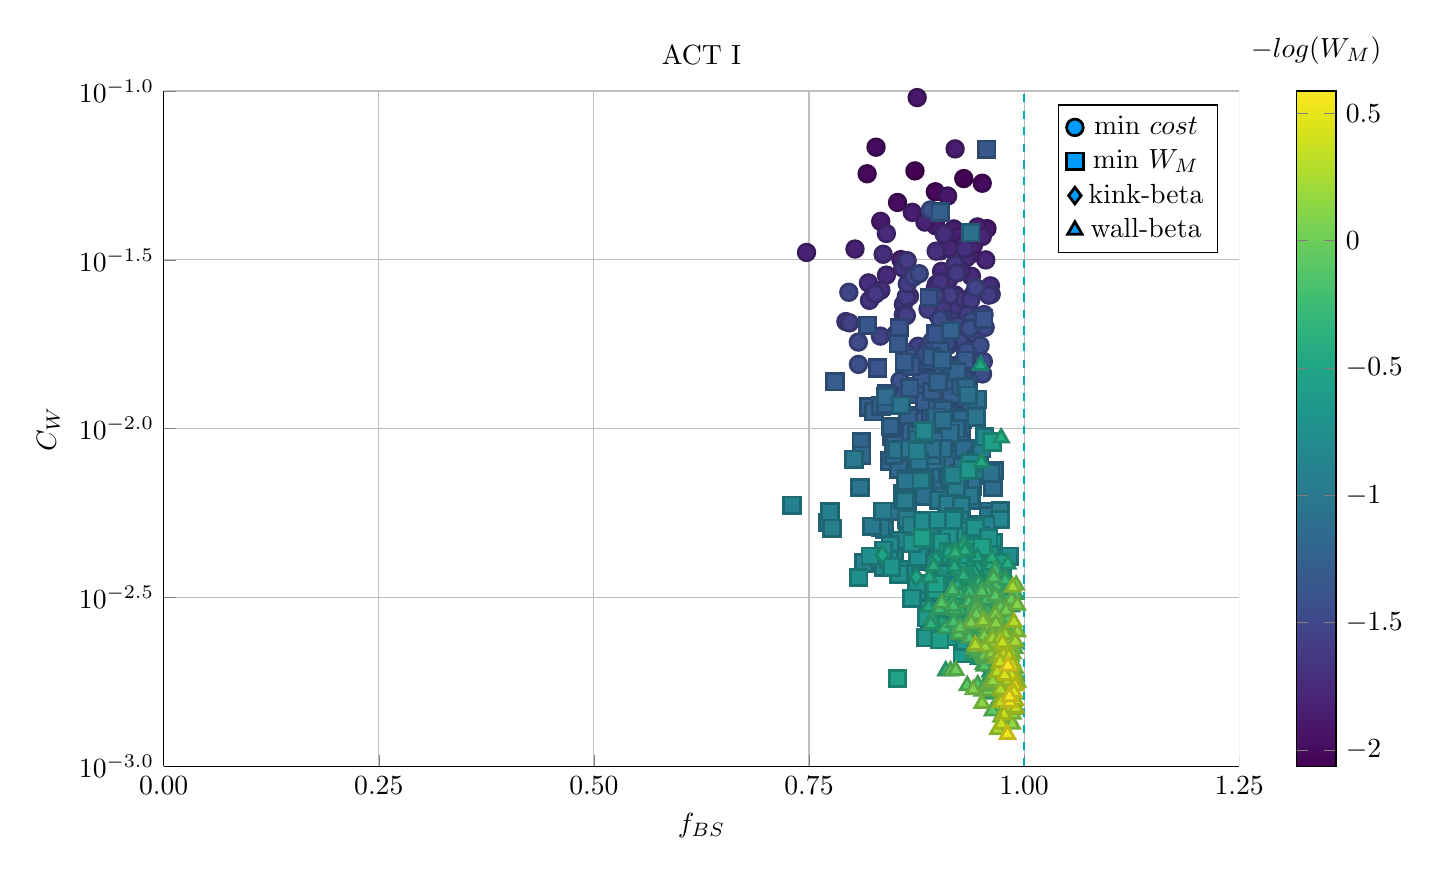
\begin{tikzpicture}[]
\begin{axis}[colorbar = {true}, height = {101.6mm}, ylabel = {${C}_{W}$}, title = {ACT I}, xmin = {0.0}, xmax = {1.25}, ymax = {0.1}, ymode = {log}, xlabel = {${f}_{BS}$}, {unbounded coords=jump, scaled x ticks = false, xticklabel style={rotate = 0}, xmajorgrids = true, xtick = {0.0,0.25,0.5,0.75,1.0,1.25}, xticklabels = {0.00,0.25,0.50,0.75,1.00,1.25}, xtick align = inside, axis lines* = left, scaled y ticks = false, yticklabel style={rotate = 0}, log basis y=10, ymajorgrids = true, ytick = {0.001,0.0031622776601683794,0.01,0.03162277660168379,0.1}, yticklabels = {$10^{-3.0}$,$10^{-2.5}$,$10^{-2.0}$,$10^{-1.5}$,$10^{-1.0}$}, ytick align = inside, axis lines* = left,     xshift = 0.0mm,
    yshift = 0.0mm,
    axis background/.style={fill={rgb,1:red,1.00000000;green,1.00000000;blue,1.00000000}}
, colormap={plots}{rgb=(0.26700400,0.00487400,0.32941500), rgb=(0.27794100,0.05632400,0.38119100), rgb=(0.28291000,0.10539300,0.42690200), rgb=(0.28229000,0.14591200,0.46151000), rgb=(0.27619400,0.19007400,0.49300100), rgb=(0.26514500,0.23295600,0.51659900), rgb=(0.25042500,0.27429000,0.53310300), rgb=(0.23360300,0.31382800,0.54391400), rgb=(0.21813000,0.34743200,0.55003800), rgb=(0.20123900,0.38367000,0.55429400), rgb=(0.18555600,0.41857000,0.55675300), rgb=(0.17117600,0.45253000,0.55796500), rgb=(0.15772900,0.48593200,0.55801300), rgb=(0.14618000,0.51541300,0.55682300), rgb=(0.13374300,0.54853500,0.55354100), rgb=(0.12346300,0.58168700,0.54744500), rgb=(0.11948300,0.61481700,0.53769200), rgb=(0.12632600,0.64410700,0.52531100), rgb=(0.15014800,0.67663100,0.50658900), rgb=(0.19109000,0.70836600,0.48228400), rgb=(0.24607000,0.73891000,0.45202400), rgb=(0.31192500,0.76782200,0.41558600), rgb=(0.37777900,0.79178100,0.37793900), rgb=(0.45867400,0.81636300,0.32972700), rgb=(0.54552400,0.83803900,0.27562600), rgb=(0.63690200,0.85654200,0.21662000), rgb=(0.73088900,0.87191600,0.15602900), rgb=(0.81457600,0.88339300,0.11034700), rgb=(0.90631100,0.89485500,0.09812500), rgb=(0.99324800,0.90615700,0.14393600)}, colorbar style={title=$-log( W_M )$}}, ymin = {0.001}, width = {152.4mm}]\addplot+[scatter, scatter src=explicit, only marks = {true}, color = {rgb,1:red,0.00000000;green,0.60560316;blue,0.97868012},
draw opacity=1,
line width=0,
solid,mark = *,
mark size = 3.0,
mark options = {
    color = {rgb,1:red,0.00000000;green,0.00000000;blue,0.00000000}, draw opacity = 1.0,
    fill = {rgb,1:red,0.00000000;green,0.60560316;blue,0.97868012}, fill opacity = 1,
    line width = 1,
    rotate = 0,
    solid
}] coordinates {
(0.8731583161087341, 0.057989258974827255) [-2.064962192389615]
(0.9298987639499251, 0.05502891594035146) [-2.050664082112704]
(0.8175467269590015, 0.05687405434298921) [-2.011767848487962]
(0.8968400727254129, 0.050297633592903325) [-2.009622310352661]
(0.8278998542362663, 0.06815552403146177) [-1.9979243426522733]
(0.9513172575512551, 0.0533071875450231) [-1.994929116630603]
(0.8528960525907812, 0.0467551640065516) [-1.9816591878685617]
(0.9110472238863242, 0.048856385398415615) [-1.9009357710890913]
(0.8756963278874996, 0.0955979106687745) [-1.9008410294477762]
(0.9568899267308207, 0.03913936102967274) [-1.8936707664226742]
(0.9038182735666613, 0.1016010514296217) [-1.88521103333311]
(0.8333207346473064, 0.04110929026091933) [-1.880964135698036]
(0.9197980139432043, 0.06737330593861776) [-1.8704830664747163]
(0.8974258881767438, 0.039880718652559814) [-1.8671602945516401]
(0.9272334069505606, 0.03552984785224197) [-1.8618595778785045]
(0.8700423982602555, 0.04370244723091091) [-1.8536550241998961]
(0.896264080513227, 0.04394725128364261) [-1.847107537048139]
(0.9182912055110312, 0.03904834505521419) [-1.845402906369208]
(0.9387755804676575, 0.03298266782702717) [-1.8299247064069584]
(0.9457850749264366, 0.03958498907028018) [-1.829338701662785]
(0.8034547513068042, 0.03404367677522339) [-1.8264739776199668]
(0.9246342918025143, 0.03712165869616768) [-1.8254736433338]
(0.9287361879267101, 0.03498163225660961) [-1.8213905780263324]
(0.8847474436704043, 0.04090408182009932) [-1.8110274827797526]
(0.856795859521427, 0.03167659938041034) [-1.8095831862560878]
(0.7471314354367964, 0.0332541407704371) [-1.8081577018045512]
(0.9410251229466832, 0.034919301353402016) [-1.8052282629113163]
(0.9553924992121228, 0.03160954199142242) [-1.794038121640695]
(0.9027109137951399, 0.03363661760525415) [-1.7922769049476923]
(0.9514525624218795, 0.03709266074378335) [-1.7862000983802733]
(0.9257525573046983, 0.03034628787303085) [-1.7852152332211932]
(0.9126142462724679, 0.03418438821960477) [-1.7772380652900426]
(0.9137711281814827, 0.028893150793615218) [-1.762233286346124]
(0.9229419485607372, 0.029679536940788936) [-1.757619916562725]
(0.9387544327064793, 0.028272317581563573) [-1.7541482977205345]
(0.8399908446535905, 0.028494444671935192) [-1.74919856251915]
(0.9330063198718748, 0.032094980075716116) [-1.747084370881807]
(0.9063829544808711, 0.027966816127232584) [-1.7470546081344984]
(0.8399078918577088, 0.03785249464890645) [-1.7442108348393488]
(0.9126714878088179, 0.027768727927201312) [-1.7420526933193456]
(0.9040493373469549, 0.029239023742660956) [-1.7395327755770893]
(0.9263873900569953, 0.02939344172802083) [-1.7194177486385185]
(0.8190620873895971, 0.027016419839008144) [-1.719386672725069]
(0.9608485147869371, 0.026478979134740822) [-1.7169068826642142]
(0.89672100112121, 0.02601353823911718) [-1.7158560236705473]
(0.8335103664153296, 0.025717415997762467) [-1.7110377836485957]
(0.8361586338341608, 0.032841764983913675) [-1.7108276685719623]
(0.9070013488697205, 0.03768314208183477) [-1.709665884336222]
(0.9311210648665087, 0.03408240796385454) [-1.6986723169730482]
(0.8977814047825817, 0.033552619629254835) [-1.6917720816198454]
(0.8979339043288382, 0.026734133388752808) [-1.6830702313615284]
(0.920096146584318, 0.024877717887061637) [-1.6818639287776478]
(0.9190311076672922, 0.02919080947335078) [-1.667258093217262]
(0.902083744032784, 0.027165378557205796) [-1.665200843447988]
(0.8202655212580311, 0.023985969206987357) [-1.66217138739501]
(0.9379149059771016, 0.024369099798012727) [-1.6616987570129709]
(0.8590574607971557, 0.029926873126084393) [-1.6608624949428865]
(0.8597162435331946, 0.023350604040071967) [-1.6542636311884442]
(0.9185584139892619, 0.022733615388835223) [-1.65363376409944]
(0.9200377378936719, 0.03074573955404929) [-1.6499261984079694]
(0.8989974045287558, 0.021769443299714454) [-1.6484233463349593]
(0.8718753959829374, 0.02860848134593445) [-1.6470118901263007]
(0.9418850072877972, 0.025250245321948275) [-1.6438624547347034]
(0.9366435359764497, 0.022365397187800617) [-1.6410421830745392]
(0.8272649318479791, 0.02504410573519034) [-1.6395041975177727]
(0.8668228410582832, 0.024666593634892982) [-1.6243573447802595]
(0.9217351814736208, 0.028901356853889247) [-1.6188313334564102]
(0.8968900959049646, 0.024870707244338257) [-1.6157329420330897]
(0.9049171939361385, 0.022969634317882806) [-1.6146571362099007]
(0.9307115846083037, 0.024077156878874784) [-1.614148731181496]
(0.9379312484272587, 0.02402881672676728) [-1.6095005691221438]
(0.9477409900819321, 0.0213102395674736) [-1.6092867324036153]
(0.9128640642999587, 0.020843342235322113) [-1.606635632554758]
(0.9617530768801122, 0.025003512509316483) [-1.606526739230697]
(0.8641075780272186, 0.03145376067268257) [-1.6054664027569479]
(0.7928641998948353, 0.020759493215449603) [-1.6036698390910544]
(0.8630240833375084, 0.024586269311698983) [-1.6025929165372244]
(0.8899699098575933, 0.02396900141580778) [-1.601873650665826]
(0.8595397653225256, 0.02173039511371947) [-1.6001281654735064]
(0.9588881971051215, 0.024851813061130205) [-1.5927988322260167]
(0.8642522328187694, 0.026860543755753686) [-1.5904529771214546]
(0.9134881848837252, 0.024815855265830314) [-1.58811206678891]
(0.8882619509730663, 0.022585530362625818) [-1.5852343487621334]
(0.8631856102877079, 0.02162169573243782) [-1.582687569840729]
(0.934056025980493, 0.02173125537760968) [-1.5805683995222133]
(0.7970138681074869, 0.020578686019115836) [-1.5616593837754646]
(0.8974438078752208, 0.0247399675666878) [-1.5545497681585543]
(0.9168089411359047, 0.02087834014908712) [-1.5504546678365727]
(0.8766721420501833, 0.01754547485137827) [-1.5489678431306624]
(0.8329698462406033, 0.01880088916330476) [-1.547222990629499]
(0.9313401534450555, 0.017954533760819902) [-1.5437410994768777]
(0.9063113702518492, 0.021211686613504643) [-1.5255698667472164]
(0.871445793631103, 0.028101067905464787) [-1.5206640942520917]
(0.9397631726706575, 0.018515106277898145) [-1.520578888956828]
(0.9077584139943392, 0.018879475562532277) [-1.5201607060653763]
(0.9227664842238432, 0.020162124791840028) [-1.517243514284296]
(0.9412253367039378, 0.01912604393689236) [-1.516001511335505]
(0.953452460582578, 0.02177699641289885) [-1.5127243295363797]
(0.9438615045031515, 0.02615640746740752) [-1.511222347964319]
(0.7962888966851867, 0.025345623651159097) [-1.502701591213217]
(0.9547380811291167, 0.019956615828691068) [-1.4983595788523634]
(0.8505719985854386, 0.01901365472017092) [-1.4975433274881913]
(0.899430644463361, 0.01625632266260828) [-1.4955435878672778]
(0.9201283417538595, 0.01537976653434252) [-1.4952511123493635]
(0.9309774985170253, 0.01624903115292776) [-1.4946977016701204]
(0.9376439198751291, 0.01616057272154418) [-1.491361147189787]
(0.9048534492341767, 0.016312938747661723) [-1.4862110854022101]
(0.925277958000399, 0.018052944734037228) [-1.481891473964466]
(0.9003094838292903, 0.017937749457507764) [-1.4799320170752728]
(0.8781116629474472, 0.028777552856445426) [-1.4795268228707887]
(0.9124042050421236, 0.017703624284785665) [-1.4795161068178337]
(0.8874100536029459, 0.017229927300776254) [-1.478794127235364]
(0.9299945195152068, 0.015225640153675678) [-1.4782749606324128]
(0.9161525972420332, 0.01946493284584485) [-1.4776976554667125]
(0.807334203101037, 0.018049212942760347) [-1.4759943912462838]
(0.9526456571529169, 0.015822574957211174) [-1.4744008984669785]
(0.9020920748075824, 0.021091946279007116) [-1.4733664186274853]
(0.921096776641852, 0.014982074855591734) [-1.470256415712286]
(0.9197524753995123, 0.014601174892861163) [-1.4657264924078404]
(0.9100402267973169, 0.017519770324100396) [-1.4622648103665985]
(0.9105130508409129, 0.01870406946961632) [-1.460868219021949]
(0.9204517436104007, 0.014392434992574372) [-1.4591279030736708]
(0.9032916286327085, 0.015543275856823037) [-1.4545703062138304]
(0.9098830294136144, 0.0178630357754997) [-1.4542955403831663]
(0.8618675014440598, 0.016835249428121063) [-1.4541997747641515]
(0.9516794080259597, 0.014530439682258098) [-1.4536072075076547]
(0.8074486816468343, 0.015504579589192491) [-1.4354993828498328]
(0.8773929747525714, 0.01586953423288717) [-1.4354866486000943]
(0.9487796918474358, 0.01764532719276209) [-1.4338583259741084]
(0.8951064297729344, 0.014716680911382386) [-1.4312674151204707]
(0.9387703969701673, 0.020843842366528337) [-1.4287189021457418]
(0.9331988731571469, 0.01696521637728643) [-1.4273925553382794]
(0.8670248952645595, 0.013340097264397483) [-1.4261610258499517]
(0.8911158581027104, 0.04442496675209589) [-1.4254440140277673]
(0.8854310169804341, 0.016560321493328565) [-1.42482226273413]
(0.9402601091187515, 0.015724531625960336) [-1.4225696979479532]
(0.9366331162927167, 0.019897722591771878) [-1.4120206972836251]
(0.9367488229696038, 0.01984475440507257) [-1.4098371032229988]
(0.8557087953810512, 0.013870037469952114) [-1.405975517390751]
(0.9336191151312027, 0.01581527557473546) [-1.4043018072199474]
(0.8931481570105053, 0.018214076204701567) [-1.4008019722945715]
(0.934367626111147, 0.013913111202702319) [-1.4005031963379073]
(0.9006796543319567, 0.015224038090080667) [-1.3999492210183218]
(0.8593933801817952, 0.012496931004535753) [-1.395557363349914]
};
\addlegendentry{min $cost$}
\addlegendentry{min $W_M$}
\addlegendentry{kink-beta}
\addlegendentry{wall-beta}
\addplot+[scatter, scatter src=explicit, only marks = {true}, color = {rgb,1:red,0.00000000;green,0.60560316;blue,0.97868012},
draw opacity=1,
line width=0,
solid,mark = square*,
mark size = 3.0,
mark options = {
    color = {rgb,1:red,0.00000000;green,0.00000000;blue,0.00000000}, draw opacity = 1.0,
    fill = {rgb,1:red,0.00000000;green,0.60560316;blue,0.97868012}, fill opacity = 1,
    line width = 1,
    rotate = 0,
    solid
}] coordinates {
(0.9271167760173109, 0.012445200437289321) [-1.3948646368052584]
(0.8549191496769539, 0.019927789901543477) [-1.3939537522252607]
(0.8799693920666783, 0.01314653896174034) [-1.392720101640072]
(0.8840883019018607, 0.014634720837625735) [-1.3866843034020317]
(0.9282463743720426, 0.013531122619790758) [-1.3787415633888773]
(0.8297318245194182, 0.015141818780145063) [-1.3757535398176242]
(0.8899071840495214, 0.024471157047317834) [-1.3752064107168462]
(0.9035475853680445, 0.014228443732750187) [-1.3749098088959892]
(0.9529741929254569, 0.02110676259399258) [-1.3739849131883028]
(0.93235118554593, 0.012256911562073732) [-1.3738531102934994]
(0.9014172243392794, 0.01330678684829131) [-1.3663541792461127]
(0.8778691210417414, 0.012962838848090586) [-1.3656599999201575]
(0.8969519049829034, 0.019050032640328597) [-1.3610117218468736]
(0.921562044788768, 0.01466611566297692) [-1.3573180864248318]
(0.864127365726556, 0.01616266376516514) [-1.3539978288520549]
(0.8180300548996796, 0.02022915729296448) [-1.3526036033103022]
(0.892574653228103, 0.014902347651238618) [-1.3518512539407643]
(0.8859492948655946, 0.01417644155990844) [-1.3492681452505735]
(0.8815164284149091, 0.013855965560709034) [-1.3352848695692758]
(0.956613991688453, 0.06723687686431194) [-1.33496858373192]
(0.8690737446612168, 0.015329274535082153) [-1.3328072948817369]
(0.8539133069876077, 0.01784511293289267) [-1.3313031998767464]
(0.8979877157834256, 0.011330055498166416) [-1.322748849742168]
(0.8397096010237105, 0.012679730072722432) [-1.3201016347693193]
(0.9215237604303135, 0.010156176015821517) [-1.315112649155682]
(0.9318984227066295, 0.01595337289689437) [-1.3137236413304165]
(0.8968767088385567, 0.012247545212491192) [-1.3091528292933776]
(0.876709873475441, 0.010892962462246563) [-1.3069473000965746]
(0.8735967833955901, 0.012601150633741464) [-1.3031541960229396]
(0.9025134685769323, 0.01697434802243184) [-1.2931806668520078]
(0.78038272871762, 0.013783864423757071) [-1.292511856848582]
(0.9350737398239659, 0.013475298350403871) [-1.291824809841371]
(0.8849689255593775, 0.012027127277753598) [-1.2898768957519178]
(0.860694823617397, 0.01571361767672998) [-1.2891587449819788]
(0.8926973187110631, 0.016322351172723598) [-1.285228192005334]
(0.8670116920112156, 0.013183257245795298) [-1.2828328944136962]
(0.9150950258835746, 0.012671641181110452) [-1.2825421072988568]
(0.9105634519289036, 0.010985300395990126) [-1.2800431569731807]
(0.9383400775725146, 0.011814811005805458) [-1.2782446441540516]
(0.913996516900395, 0.013863201694102639) [-1.2775473203773224]
(0.9121820439610082, 0.015027301664507256) [-1.2767406237155188]
(0.8723989867889326, 0.010547820414817374) [-1.2761629204758234]
(0.8902896550731525, 0.009931862296416103) [-1.2758557981370644]
(0.9158421037667931, 0.009498142916512152) [-1.2757288295353457]
(0.8925383407041332, 0.012893329705558294) [-1.2744847837776876]
(0.8192563180348535, 0.011606796760736388) [-1.2735549705057247]
(0.9161057579223539, 0.01475971281582095) [-1.2726652036752184]
(0.9025687723545689, 0.04385064317226166) [-1.2725563531490864]
(0.9176423466313344, 0.00956494266353577) [-1.2722662263080966]
(0.8991796141625694, 0.01145377372543799) [-1.2700642653169505]
(0.920538508471723, 0.010133330755881341) [-1.2679487567038392]
(0.9165797234269246, 0.009123134682627944) [-1.2616514169448798]
(0.8634478673767971, 0.009795622872305737) [-1.2594613969180772]
(0.8652451113775445, 0.01079410220229538) [-1.2586087657706206]
(0.8974734735996593, 0.0088934936775186) [-1.2559318752922384]
(0.8972097836781053, 0.00878637495619299) [-1.2524032337696909]
(0.9146956817162654, 0.01954536936309829) [-1.2500915845956104]
(0.9266577237247744, 0.013401347258256273) [-1.2491939573401372]
(0.9060566912781703, 0.009287974505863453) [-1.2465820537241712]
(0.8461463841435856, 0.009508338508488968) [-1.243935477994714]
(0.9180394857798562, 0.009032887794110376) [-1.240347841326793]
(0.8562897903410046, 0.008840699433936929) [-1.2384200469490936]
(0.9157222626166746, 0.008939458902182977) [-1.2370382372338191]
(0.8774564802835889, 0.009500681442262262) [-1.234594616796923]
(0.8997140678463201, 0.013750191876996646) [-1.2345143468522275]
(0.8255430755693288, 0.011226325606846698) [-1.2333943003160397]
(0.8338112522107382, 0.011680936250442807) [-1.2317476546541377]
(0.8685627242411781, 0.009765734724622308) [-1.2309520865359098]
(0.8971615157301666, 0.010568167602651573) [-1.230822839476929]
(0.838843805052853, 0.011811831633915183) [-1.2301871906487212]
(0.8789107801666443, 0.00916985873364138) [-1.2298215185804844]
(0.8919234914358547, 0.008206632432567867) [-1.2262871207474173]
(0.9214414379326734, 0.008184707349761693) [-1.2251252918595636]
(0.9275904428089702, 0.009543389942473697) [-1.2247092653793519]
(0.9143231802086956, 0.008412326051837992) [-1.2226672824447191]
(0.9216123853497962, 0.014763516356953353) [-1.2220223430792259]
(0.9044002301485325, 0.01597138256674089) [-1.219978616872189]
(0.9027130017667216, 0.00839744989573872) [-1.219457473300232]
(0.9211645176611111, 0.010746093594156849) [-1.2188777190787354]
(0.8786258539538101, 0.008033832445301942) [-1.2169302951859435]
(0.8494484079850726, 0.008975990584934701) [-1.21686127758645]
(0.9221310289995527, 0.009398677017548424) [-1.2167616565149533]
(0.84466182771518, 0.010149128207773273) [-1.2150613565699149]
(0.9208861119140008, 0.008396583729988576) [-1.2136335595316654]
(0.9053639683207135, 0.01140115444851449) [-1.213449396676557]
(0.9018392826470298, 0.00807858566271283) [-1.2090424219749658]
(0.8107793492157458, 0.009150247244763429) [-1.2068811791719494]
(0.9260034079845344, 0.00910352225246922) [-1.2043566377787012]
(0.8442941324782789, 0.008030436201599676) [-1.203115426690566]
(0.8621899253038897, 0.00829525893430832) [-1.2026712887263624]
(0.9475382029731105, 0.0076660148584983805) [-1.1966917975345508]
(0.9152752571057894, 0.010646380662135389) [-1.1947338618724224]
(0.8593153099539642, 0.008370016806452012) [-1.1927672386559536]
(0.8544491568392304, 0.007597051992083297) [-1.1848263349710841]
(0.8757227850487023, 0.009575551810758922) [-1.1808013668049147]
(0.9251889351463798, 0.007741558979980694) [-1.1794231767577772]
(0.811212783417515, 0.008342037909753687) [-1.178329489639351]
(0.9043967242186975, 0.01061614690368138) [-1.1776120518997013]
(0.9187473583725516, 0.008028594314197455) [-1.1770966259473905]
(0.9325685727720403, 0.013299033663900294) [-1.1736537021823468]
(0.8904003702289742, 0.008292790623650929) [-1.1709553925305785]
(0.8482856059746025, 0.008348409776511478) [-1.1702773251540795]
(0.9134364460032778, 0.008067808434749702) [-1.167112460757148]
(0.9244771021986321, 0.007367175811164478) [-1.1651375230967302]
(0.9279526851295172, 0.010664194028670942) [-1.164965492702215]
(0.8973994172179647, 0.010811857237065516) [-1.16397652023692]
(0.9394191821156371, 0.007049158619545943) [-1.160208221592745]
(0.9265691326442036, 0.007024176248113807) [-1.1587174467250145]
(0.9280658506320641, 0.007717544771526665) [-1.1570209420480233]
(0.9303231791026377, 0.008736514143459023) [-1.1478957642324041]
(0.9006608632246583, 0.009218200163918491) [-1.1469002727681683]
(0.9411405362226928, 0.007253865516894526) [-1.1400875045234886]
(0.9650109382613667, 0.007524944567097975) [-1.1391691710531666]
(0.8391428834450059, 0.012439153670574864) [-1.1379833555384578]
(0.9262309554101665, 0.0069967893818347416) [-1.1377170826120309]
(0.9208209619324543, 0.010002872629106504) [-1.1340145582937184]
(0.9637544328450613, 0.006715015712432569) [-1.121639283140209]
(0.9400709731105008, 0.006729229846129435) [-1.119539806519794]
(0.9014204193264993, 0.00641032554112888) [-1.1190022218812188]
(0.8923890653126869, 0.0073365166963547295) [-1.1185629451884402]
(0.882251161202865, 0.009102128960090845) [-1.1149656449984597]
(0.9018049683243878, 0.006567068570130298) [-1.112782188839356]
(0.8853454131125228, 0.006812914645648147) [-1.1117603631555923]
(0.9391048518724179, 0.006254604192766126) [-1.1083219728450635]
(0.87681385329431, 0.009301357270274212) [-1.1068629047281389]
(0.9244645109147069, 0.006851310091732623) [-1.1063474773659798]
(0.9141312650810365, 0.009696451234501371) [-1.1001422615629064]
(0.8978057921219315, 0.008046176359548657) [-1.0997982629203031]
(0.9209594912343368, 0.0061171437643153005) [-1.098670828295362]
(0.9054893907504951, 0.010596545096731845) [-1.0986241378865482]
(0.8877315508685263, 0.008577289597829926) [-1.0966387184251443]
(0.9452449245553554, 0.008169596287759642) [-1.0964883993749868]
(0.9132214581978662, 0.007121767916062895) [-1.0945790180182455]
(0.9150525541207138, 0.007187659319073351) [-1.0926081998530923]
(0.9058219953417993, 0.008724343791351657) [-1.0921043707901013]
(0.947802134523662, 0.008329953635747183) [-1.0913882990792323]
(0.8933038303627091, 0.008322658254688352) [-1.0910813694377977]
(0.8833011988886175, 0.006304319577189367) [-1.0901679951720686]
(0.8929811603643258, 0.008690684170777426) [-1.089367091074117]
(0.9145080171681728, 0.006583412820443741) [-1.0891727565542524]
(0.9453955802025471, 0.012211134116054666) [-1.0880555961261078]
(0.9350836555291349, 0.012548811552576346) [-1.086936622940194]
(0.8589137292175502, 0.0064141553047330985) [-1.0863825614156546]
(0.8836849391290048, 0.0071097507635516565) [-1.0751044594117714]
(0.9610484127018367, 0.007374731494224653) [-1.0737380492352289]
(0.9389985571359603, 0.006145695209859947) [-1.070616517292677]
(0.9379977248665374, 0.03802674603286673) [-1.069913767001807]
(0.9213417260466619, 0.005970957417198659) [-1.0690750828665614]
(0.8548598275117848, 0.005698307632946107) [-1.0678680329287458]
(0.8522098522639113, 0.008661247168726348) [-1.0674080884082333]
(0.9439305152507809, 0.010817648781713476) [-1.0654260064541108]
(0.8567559640448742, 0.011722467292523471) [-1.065193792118979]
(0.920196530172107, 0.005714167148636787) [-1.0629774807936423]
(0.8640983076229167, 0.00711622998416048) [-1.0618319340909603]
(0.8592709820297094, 0.006173537615536586) [-1.0600703364411528]
(0.8583017671103392, 0.006233626320552047) [-1.0598646582955382]
(0.8841777194347801, 0.009626390481863662) [-1.0577742882294356]
(0.9122660365302591, 0.005936752040130104) [-1.0548470198030315]
(0.9587389518915752, 0.0056904737038728165) [-1.0541768592648042]
(0.9108628990594947, 0.006032343424076769) [-1.0487285499150356]
(0.9584682101650461, 0.005521470027251347) [-1.0462570464475487]
(0.9173449278328639, 0.0070995694405497235) [-1.0460234006078977]
(0.8628552558040238, 0.007007981654725635) [-1.0452759731087355]
(0.8668509459578728, 0.008683290730999459) [-1.0445119467109005]
(0.9105499342272777, 0.0055299967565469975) [-1.0384000215358105]
(0.8638198429570266, 0.005998532550171044) [-1.038305441802928]
(0.9208568729989152, 0.00528018761380554) [-1.0347714947666997]
(0.8093436631281515, 0.0066967057377454575) [-1.0308440378796533]
(0.8779579874197121, 0.008036724741540775) [-1.0305940259463149]
(0.906869624199176, 0.0062926123227946265) [-1.025221203256898]
(0.900789950373511, 0.0061379044438670954) [-1.0179285117664867]
(0.9375398126250842, 0.006334972879805434) [-1.0176162076457083]
(0.8024708047377667, 0.008112959181062486) [-1.0169975029536151]
(0.8375801334207545, 0.005049047597761542) [-1.0141985821053012]
(0.9324121317714827, 0.005064450169828918) [-1.0124724404696706]
(0.833350555301248, 0.005088814715939496) [-1.0103391716309778]
(0.9513980291319009, 0.004962576605235948) [-1.001427881081934]
(0.9271181895900452, 0.005884671104664021) [-0.9993824808081277]
(0.9099503941424658, 0.005418776785282774) [-0.9941634259261274]
(0.7720181731709707, 0.005280889139989257) [-0.9936318009336389]
(0.9505960598919263, 0.008723874856120134) [-0.9908776434018548]
(0.8943895369875628, 0.00491490634866398) [-0.9892483689799706]
(0.9417125317554466, 0.004961736780563244) [-0.9883704068819422]
(0.8233418299878267, 0.005137841489967903) [-0.9826953741849849]
(0.8934787894059866, 0.004754734001145322) [-0.9811279654336956]
(0.9403526918266536, 0.004647560340984803) [-0.9793471772630553]
(0.9723583859212274, 0.005703060525950649) [-0.9776886993834442]
(0.8611589318505539, 0.006131488667777248) [-0.9769724317666026]
(0.9410654966962836, 0.004745131633522655) [-0.9769267723302241]
(0.9399901789088603, 0.005212687153670182) [-0.976835072767447]
(0.9567462107415136, 0.0046034051010616075) [-0.9752013352458598]
(0.8636848687114632, 0.005388412680270176) [-0.9746899157531883]
(0.9075358432123548, 0.0045774223618013105) [-0.9727431242330735]
(0.9447314559272533, 0.004552413603526284) [-0.9703638528440552]
(0.9414650087723526, 0.004525683131963228) [-0.9678062840180223]
(0.8357492652861911, 0.005692276004720247) [-0.9676725483675591]
(0.9005181216481226, 0.004498229501695765) [-0.9651637505902915]
(0.9206601577164616, 0.0067323238980037245) [-0.961259110326393]
(0.9083905113541957, 0.004736392493078221) [-0.9563360314157324]
(0.9301172641173069, 0.004854184151533866) [-0.9558845590306136]
(0.9194947604180831, 0.004573806166601441) [-0.9532763546481751]
(0.941953192362469, 0.004793440229443098) [-0.9511957035164516]
(0.8806212569679992, 0.004877743614014347) [-0.9508596108314747]
(0.9329503575731299, 0.004350998493140003) [-0.9507110729257874]
(0.911454495262883, 0.006001608290604688) [-0.949683613164744]
(0.8879558751803653, 0.004290521076860756) [-0.944632180714094]
(0.9184319984465406, 0.0043767749507575135) [-0.9438112967734156]
(0.9271750473353343, 0.005920276984804288) [-0.943373672256531]
(0.9105611701686498, 0.005363684807666859) [-0.940593168106771]
(0.7767420971999245, 0.005068452256325543) [-0.9348384496596517]
(0.9038987139905713, 0.0049263739241811695) [-0.9347532688355591]
(0.8759023691861031, 0.008601524715605227) [-0.9342019527454238]
(0.8549702147859954, 0.004640144515353838) [-0.9329513708540818]
(0.8803983184588043, 0.0070257271621669455) [-0.9316183752161744]
(0.9259016565967537, 0.005358998371858679) [-0.9286370269103483]
(0.9616193719002063, 0.00413086470485901) [-0.9281631121842467]
(0.8741693390281038, 0.004765635288464319) [-0.9277381641373396]
(0.8490865721871718, 0.0040620137628436526) [-0.9208635313499342]
(0.8814246252669371, 0.0040488305993979234) [-0.9194517468501666]
(0.7743381134865549, 0.005678582545669974) [-0.919260894818004]
(0.8140652070684143, 0.0040019705744028635) [-0.9143960307834678]
(0.8956167430991006, 0.005105193674380799) [-0.9143339304202898]
(0.923307386920103, 0.004202079139621733) [-0.9117699942132877]
(0.9090872570665293, 0.004239308070694324) [-0.9111513250328139]
(0.9186515311897197, 0.005481038677141083) [-0.9106272870974846]
(0.8651143294304927, 0.004774812507931078) [-0.9099002226686804]
(0.9212576993079015, 0.003944067969601837) [-0.9080665243282653]
(0.9288275574225838, 0.004788438955058866) [-0.9070188756981697]
(0.9170518000340987, 0.007279773971914604) [-0.9043577198452432]
(0.9063089707483508, 0.004734796732954004) [-0.9038476343568516]
(0.9417824172363041, 0.007562673512498189) [-0.8994655785667166]
(0.7301551050698963, 0.005931441653675227) [-0.8989662338456113]
(0.9221426597591885, 0.003977844960348454) [-0.8984429206195617]
(0.924185246169707, 0.003852765847835788) [-0.8978947560680902]
(0.9113180230450746, 0.003844792233549059) [-0.8969950165065196]
(0.915991064143121, 0.0038178462182025725) [-0.8939405705697983]
(0.9184306750512461, 0.004330108994839308) [-0.8939109716982566]
(0.8906172680403811, 0.004992871742589902) [-0.8925148817167516]
(0.8413904437613173, 0.003881299542388103) [-0.8913217265447397]
(0.9127227138669043, 0.003772719391214399) [-0.8887766390600081]
(0.908016086635955, 0.003988034719656209) [-0.8874455768491046]
(0.9229973452568307, 0.003741945120882656) [-0.8852195535706585]
(0.9042193119427263, 0.0039058028277476073) [-0.8842325860222515]
(0.9626746195716175, 0.0037216011971632503) [-0.882851972521222]
(0.9136705428571793, 0.005315372520692716) [-0.8819881369375219]
(0.9255182413778642, 0.004466619068705632) [-0.8808109550697729]
(0.9332929151781738, 0.004730802817477606) [-0.8806633070174894]
(0.9455320084521668, 0.005113228457075696) [-0.8805814649771261]
(0.9059749221374921, 0.004582507032171267) [-0.8799678258438864]
(0.8687604466888538, 0.005177586923248842) [-0.8768550082578233]
(0.906638161832524, 0.0037611740992579295) [-0.8726983150888058]
(0.9142503324644239, 0.003993806119831429) [-0.8703497234695906]
(0.9005945327194729, 0.0045270286179628335) [-0.8696853700725911]
(0.9125504162559055, 0.004726535412937384) [-0.8641851323647479]
(0.8894648886019335, 0.004089711851258383) [-0.8640642580417203]
(0.84906414633368, 0.004221088787393515) [-0.8560530688301973]
(0.9539183047560731, 0.009465725470453552) [-0.8558368077947285]
(0.8365167684350138, 0.003886605388747585) [-0.8512125553695333]
(0.9717681447799739, 0.005381883944145375) [-0.8506650866802525]
(0.9413045252603143, 0.0034368070052375275) [-0.8482772851581519]
(0.9371247405745184, 0.007913375166879979) [-0.8464932034376795]
(0.9553776236479619, 0.005205559212542438) [-0.8445031740165281]
(0.9335984452174588, 0.003401911815632122) [-0.8438451898892435]
(0.899362439922284, 0.0036969679593135867) [-0.8422027975238203]
(0.9073351601479548, 0.003987547217632283) [-0.8387200271046066]
(0.8562092207533517, 0.004668264864015146) [-0.8364691763469672]
(0.8837759321999247, 0.009844996004785781) [-0.8348845112947673]
(0.9527366094531792, 0.0042937690240102055) [-0.8334732362359846]
(0.9489776318197072, 0.004829578534215681) [-0.8314604487141729]
(0.9406793011442216, 0.0033045292752156012) [-0.8312317421172319]
(0.9066275099303774, 0.003944865613295989) [-0.8300993342247266]
(0.9525847470320502, 0.0036964164829665054) [-0.8257124339268005]
(0.8444119719816215, 0.004543282198622211) [-0.8240402889058517]
(0.8428732433620125, 0.004091458079546767) [-0.8237101255156289]
(0.8792038820199741, 0.0044798519520400275) [-0.8212814607963961]
(0.9128010485164441, 0.003865354216978021) [-0.8184309573457651]
(0.9408107529966464, 0.003517618433797349) [-0.8179460037153172]
(0.907201661370005, 0.004172133397045878) [-0.8177471845862596]
(0.9147419729006552, 0.0032035011715418273) [-0.8177470190925474]
(0.9341737972997356, 0.00486116253252262) [-0.8115196740923352]
(0.880427881452171, 0.003291086034139362) [-0.8109601097483452]
(0.9369616057293777, 0.003137434005415254) [-0.8086967395269018]
(0.9368507058055328, 0.004970208362256673) [-0.7960351903235757]
(0.8759951589174462, 0.004399209393210064) [-0.7927306784842179]
(0.8824674295611945, 0.0053371866278534704) [-0.7914765499147394]
(0.9379258499987612, 0.003498945953927069) [-0.789558366829936]
(0.9198630378378857, 0.0036511274139089086) [-0.7884146729758114]
(0.8944594126549716, 0.003059756391991388) [-0.780563955995713]
(0.8365394691215563, 0.004362695965775012) [-0.7773019949176746]
(0.9490480155902238, 0.0033800793800363477) [-0.7771403289080958]
(0.9131766240023282, 0.0038433908405004595) [-0.7759893078752428]
(0.9174522110836529, 0.005361590568500423) [-0.7757750986160458]
(0.9828063504707286, 0.004188332285621625) [-0.773903866721892]
(0.860373325745603, 0.003814507127921371) [-0.7720119659547495]
(0.916412698271093, 0.004563472793394545) [-0.7712260807781841]
(0.8993603428221363, 0.005353933823001906) [-0.763713355476829]
(0.9229671461890366, 0.00443577956251074) [-0.7611487713118793]
(0.9135746793667092, 0.0035425697821227136) [-0.7583244805207935]
(0.910163554471783, 0.004316533455984555) [-0.75431667125663]
(0.9530775482444933, 0.004013911959896482) [-0.7523987856492388]
(0.8765992248443446, 0.004167145198855743) [-0.7521837169110341]
(0.8211767177946366, 0.00419041579250737) [-0.7520281092582939]
(0.899188988809008, 0.004640432958808489) [-0.7480037221630257]
(0.9196475384979264, 0.004637571540936418) [-0.7479709949279421]
(0.941544518760215, 0.0029690205808463126) [-0.7433492218430673]
(0.8548068550317491, 0.00371133233538681) [-0.7429682997042104]
(0.9076295967230273, 0.0037176890833071395) [-0.742916937139166]
(0.9629606418977977, 0.003573548669295098) [-0.742391688221943]
(0.9132986441445263, 0.004342699202151464) [-0.7387214685527604]
(0.9425549117040624, 0.004120352722007335) [-0.7376833551276831]
(0.8876167102132334, 0.0029344519800280494) [-0.7361332571045444]
(0.9192007895561155, 0.0026407580062505036) [-0.7338507300143334]
(0.9190838352844859, 0.004642553663675521) [-0.7338020684083535]
(0.8076734375543824, 0.003625959959243182) [-0.7337899099402782]
(0.8755348906962087, 0.003471864499773886) [-0.7327475728465653]
(0.9192982155145527, 0.004787324827841368) [-0.7317731615704781]
(0.9128657943764739, 0.0032492446650530782) [-0.7295946657832332]
(0.9643502521670281, 0.004590135412859294) [-0.7278656799085517]
(0.9436063499469458, 0.002781573765952152) [-0.7275349704092896]
(0.9124911104830998, 0.004786847520366514) [-0.7260638209608133]
(0.8701208160624356, 0.0045831738993045434) [-0.7223530950014921]
(0.8903186381182336, 0.002706327638391427) [-0.7222465976506431]
(0.9221605488926754, 0.0038384358624846005) [-0.7206838995228373]
(0.8697565045491886, 0.0031485580487720824) [-0.7200286244342213]
(0.9304077214790845, 0.0025439466913436885) [-0.7176301464195668]
(0.9277282929298999, 0.0032994837811560433) [-0.7172574131133485]
(0.9083357619132455, 0.0029608346461731517) [-0.7146734939586027]
(0.9386095594667047, 0.0038416894509805963) [-0.7135338154993714]
(0.9622893760246558, 0.003978944435631734) [-0.7134219342397831]
(0.9244732248388806, 0.00294062590420396) [-0.7111824287105687]
(0.9074754137233341, 0.002616774757125684) [-0.7110478679106434]
(0.9283660526071763, 0.002703036682855945) [-0.7101349740556314]
(0.9333747341388989, 0.0038042134944218514) [-0.708793386355897]
(0.9430505809327492, 0.005100030907026268) [-0.7086868054853989]
(0.9427900983410764, 0.0029638877995658438) [-0.7060021380009439]
(0.9398200782334812, 0.00420966050281472) [-0.7051679285913526]
(0.9604861518997936, 0.004243872080162761) [-0.7047135863350958]
(0.9589708628544776, 0.004746158897630676) [-0.7042552774527877]
(0.8457887824363216, 0.0038984799726810644) [-0.7040543449813873]
(0.9446655949709295, 0.003681874907434521) [-0.7029065147187739]
(0.9255802437476592, 0.003518446922920876) [-0.7024908064183792]
(0.9430578726532933, 0.0031358132900712187) [-0.7020173640529951]
(0.9358114830098702, 0.0034846556769238916) [-0.7002858883929466]
(0.9154923073284251, 0.002420499336307095) [-0.6886136022852183]
(0.9487125552664237, 0.0030008632151973602) [-0.6883840449068117]
(0.9749351638619993, 0.0036390786158231932) [-0.6856303672495035]
(0.9354490208131545, 0.0075440190367227515) [-0.683929391159688]
(0.8861740952059259, 0.0024047709432785456) [-0.6820666452179769]
(0.9399550230633152, 0.003179486303873929) [-0.677506260008208]
(0.9172222823672502, 0.002743556277657468) [-0.6766480250628556]
(0.8971448208467913, 0.0033449553430014638) [-0.6742373084561588]
(0.9498796899572547, 0.003589950489194691) [-0.6693580918378859]
(0.9614003416076418, 0.0027885517140979043) [-0.6663261681981373]
(0.904051942834427, 0.004612234783079175) [-0.6640820182002938]
(0.8870769402218344, 0.002756794030954554) [-0.654540142215377]
(0.9145144637231343, 0.003011986481013787) [-0.6541170476368723]
(0.9386740677642995, 0.0023920692653461198) [-0.6479269306921259]
(0.9272166472611978, 0.002907917303840169) [-0.6474513086378696]
(0.9652245577162768, 0.003970372686667843) [-0.6471618340133566]
(0.9361938078592776, 0.004183393535167865) [-0.6464557691155365]
(0.9282205063877679, 0.0021562827004047414) [-0.645827839166682]
(0.9428246002353234, 0.003935863383612764) [-0.6392562670118296]
(0.9332729807874064, 0.0033071434441903505) [-0.6390324015661447]
(0.965299692734038, 0.0029382720604000773) [-0.6356690770784437]
(0.9307544297265398, 0.003213331172803855) [-0.6356557512792106]
(0.9020078833291566, 0.0034338634182182544) [-0.6319127156425483]
(0.9637226872809501, 0.0026258384701233024) [-0.6311782107023105]
(0.9311304196250344, 0.002344563264707828) [-0.6306618545653738]
(0.9362327301699095, 0.0043309424812136305) [-0.6294646208449958]
(0.9571595789927293, 0.0035648943963739244) [-0.6281694872206178]
(0.9373951586764807, 0.004473909353971782) [-0.623997332545462]
(0.9246735358540317, 0.003055298672515709) [-0.6239428210926011]
(0.9604091908555257, 0.0033667157021052925) [-0.6220841804266346]
(0.8970165492513017, 0.003322033041865016) [-0.6194634144361497]
(0.9463845319434011, 0.0026017333836386653) [-0.6157020019788386]
(0.963381254766795, 0.002981595770740583) [-0.6128668873662166]
(0.9386459319770583, 0.0029654442870923124) [-0.6087223349615605]
(0.9378475201084454, 0.0027835646988952733) [-0.6079986647506345]
(0.9662961539484464, 0.0035338295468618167) [-0.607409669430742]
(0.9676799600416237, 0.003208776600520151) [-0.6057755138787592]
(0.9548162111293393, 0.0024649747969395317) [-0.6023349029229402]
(0.9437686876752717, 0.00428654565390444) [-0.6021966320137805]
(0.9313542688063162, 0.0036421375219878684) [-0.601256050165278]
(0.9810116318859735, 0.0032082112461564497) [-0.6004710736804056]
(0.9210211525451228, 0.0033480033632593445) [-0.5989376185886022]
(0.9261414327388798, 0.004184088897695592) [-0.5988379503314065]
(0.9451747550689351, 0.0021588377429705994) [-0.5983904370889932]
(0.9603531355012247, 0.002371262429759035) [-0.5972702626291994]
(0.9145691707746888, 0.003153537233065522) [-0.5971677630195633]
(0.9332687303609898, 0.002738950954618617) [-0.5943817111698461]
(0.9017811764393036, 0.002374076549827175) [-0.5925805266117682]
(0.9529087666605505, 0.0035156750139523495) [-0.5892976849983818]
(0.8818050628541011, 0.004748358787901646) [-0.5871411238278668]
(0.9410709712036359, 0.0028576481981739026) [-0.5871026900807895]
(0.9118739529147474, 0.004310975115774645) [-0.5855555754858193]
(0.9270393774931934, 0.002622282088332502) [-0.582078933118425]
(0.9471345660347393, 0.0027290583320010026) [-0.5810302095860215]
(0.9709522317939191, 0.004011340237339877) [-0.5752080843644548]
(0.9373730580166739, 0.003188972111543657) [-0.5747894604151379]
(0.9625216290079742, 0.009121559432388153) [-0.5726182655122839]
(0.9328769641864062, 0.003781132407311784) [-0.5681761634850476]
(0.9477741047064356, 0.0035193905138756446) [-0.5675125713590323]
(0.897813303968198, 0.003476123369301586) [-0.563542896843953]
(0.9444020460316636, 0.003526213328274809) [-0.5617459654165032]
(0.9367882704708124, 0.0030283854486626957) [-0.5606455598520448]
(0.9591748673290499, 0.003698026746714474) [-0.5561768160153511]
(0.9161540099636023, 0.003037543717331452) [-0.5554794435604244]
(0.9544577117139241, 0.003123058961705477) [-0.5527929477248187]
(0.949948991371526, 0.003063222342257361) [-0.5501170234905265]
(0.9512932862322991, 0.004453634731593786) [-0.549388250021666]
(0.9704366682428202, 0.002634748468893335) [-0.5492540867532439]
(0.9706397193138688, 0.0029729026877479644) [-0.5480705365568839]
(0.9209369867443455, 0.002890688526532444) [-0.545336361217705]
(0.9727226532153145, 0.0029512333115660695) [-0.5441402349163921]
(0.9654875864077215, 0.0033237315785907802) [-0.5415522046162035]
(0.9153924411701821, 0.004254172680928966) [-0.5404988012673853]
(0.9438711844295444, 0.0028783860919469858) [-0.5391201246551751]
(0.8528119086554116, 0.0018217622549288588) [-0.5378589410507132]
(0.9399210599276655, 0.0029280615221428286) [-0.5375464729950068]
(0.9656845492175761, 0.003605866681887626) [-0.5363826507452838]
};
\addlegendentry{min $cost$}
\addlegendentry{min $W_M$}
\addlegendentry{kink-beta}
\addlegendentry{wall-beta}
\addplot+[scatter, scatter src=explicit, only marks = {true}, color = {rgb,1:red,0.00000000;green,0.60560316;blue,0.97868012},
draw opacity=1,
line width=0,
solid,mark = diamond*,
mark size = 3.0,
mark options = {
    color = {rgb,1:red,0.00000000;green,0.00000000;blue,0.00000000}, draw opacity = 1.0,
    fill = {rgb,1:red,0.00000000;green,0.60560316;blue,0.97868012}, fill opacity = 1,
    line width = 1,
    rotate = 0,
    solid
}] coordinates {
(0.9387315044574429, 0.0026801888273270944) [-0.5362477970958698]
(0.9188676920673408, 0.003015899524278956) [-0.5319316345767685]
(0.9402750910418581, 0.003937320309019732) [-0.5311726618261826]
(0.9497566997238739, 0.002676245927362068) [-0.5263288636267944]
(0.9578205337936164, 0.002870837451508785) [-0.5247247581053419]
(0.9377452621123799, 0.0036932959279301603) [-0.5234426911679817]
(0.9236521135109587, 0.0037417097390243918) [-0.5218292719861799]
(0.8746520089629003, 0.0036365094358458082) [-0.521460274671524]
(0.9465267456827315, 0.003836260132829497) [-0.5210413145984053]
(0.9414429637766969, 0.0035893000080833405) [-0.5203271708770874]
(0.8975678911738616, 0.004109858290155805) [-0.5199020238276453]
(0.95491686971008, 0.0037200592776891026) [-0.5183158834743817]
(0.9759243558794375, 0.0028015521912634306) [-0.5173345034609598]
(0.8351619950547207, 0.004230376861424109) [-0.515292403587272]
(0.911974433569001, 0.004287050052594506) [-0.512831160599956]
(0.9451890358998748, 0.00385875121306247) [-0.5125342981633305]
(0.9573604100369881, 0.0024821104525564698) [-0.5110529951676259]
(0.9255709718590797, 0.002644344245828979) [-0.5107257930504342]
(0.9014823759874409, 0.002951817009326848) [-0.5100450482708185]
(0.9342743233933991, 0.0036294488088753976) [-0.50815885357027]
(0.9386447741605193, 0.00293906318241377) [-0.5068673822722911]
(0.9434533574756855, 0.0033114367041341864) [-0.5065015706006631]
(0.9645103989085381, 0.00315022051140993) [-0.5028304672765428]
(0.965810101196494, 0.003265777243065683) [-0.5020774334996001]
(0.940852716473451, 0.002195233443131404) [-0.5006102606405294]
(0.9269508172989578, 0.0029561853413927267) [-0.4999881748262777]
};
\addlegendentry{min $cost$}
\addlegendentry{min $W_M$}
\addlegendentry{kink-beta}
\addlegendentry{wall-beta}
\addplot+[scatter, scatter src=explicit, only marks = {true}, color = {rgb,1:red,0.00000000;green,0.60560316;blue,0.97868012},
draw opacity=1,
line width=0,
solid,mark = triangle*,
mark size = 3.0,
mark options = {
    color = {rgb,1:red,0.00000000;green,0.00000000;blue,0.00000000}, draw opacity = 1.0,
    fill = {rgb,1:red,0.00000000;green,0.60560316;blue,0.97868012}, fill opacity = 1,
    line width = 1,
    rotate = 0,
    solid
}] coordinates {
(0.9637825785469384, 0.002418031031362927) [-0.498048892810302]
(0.9828868114547558, 0.0034404977503060406) [-0.4963542958643768]
(0.9417630512196451, 0.003776085604922812) [-0.49628974660312986]
(0.9492250000053065, 0.01540146473031375) [-0.4934359099515097]
(0.9528731459467576, 0.0035153091327000956) [-0.49249004910762223]
(0.9423833026459857, 0.002494247580013818) [-0.49140410679398333]
(0.9457792108846419, 0.00416125103061467) [-0.4852361666757575]
(0.9881577775397556, 0.0023204725608605052) [-0.4804115307603524]
(0.9684130895026871, 0.002093548495356325) [-0.4801206531671318]
(0.9317207652243386, 0.00284573975236386) [-0.47768993884134897]
(0.9045268350433837, 0.002672085055478309) [-0.47763997399503283]
(0.934107896081881, 0.0042968350893615405) [-0.47748483227356914]
(0.956153940041833, 0.0027283486462771588) [-0.47710934625073764]
(0.9504424943308272, 0.007954298543771714) [-0.47443162890256063]
(0.9653194212047426, 0.0034997930230070513) [-0.4730103351970393]
(0.9485975480554657, 0.003084116536456388) [-0.46957975685881903]
(0.8888799663257206, 0.002965009685568973) [-0.46566614748110147]
(0.9486063771337456, 0.0033818570105314436) [-0.4649012306603411]
(0.9370503936999514, 0.0027326785960835984) [-0.46367023078588027]
(0.9751148974972959, 0.0021589205831240984) [-0.4608405143654578]
(0.9674139205875375, 0.002909388047886919) [-0.4559980166467371]
(0.922320661557035, 0.003804219838416559) [-0.4557530150298407]
(0.9617531036033169, 0.0019740686546661367) [-0.4531031573331743]
(0.9720919152815786, 0.002865519155805154) [-0.45102557337314547]
(0.980962555274262, 0.0035904404442790834) [-0.4498801205421611]
(0.946983470396084, 0.0020770215253626836) [-0.44934749702523663]
(0.9611200201095378, 0.003946973381825038) [-0.44691387139898353]
(0.9423559591891613, 0.0021324454337363157) [-0.4467784211878218]
(0.9722802466644753, 0.0034454822663482288) [-0.44543367276420787]
(0.9783180452946528, 0.002782106060611568) [-0.4452644336485217]
(0.9196744854606606, 0.002683981555832874) [-0.4442292803657962]
(0.919083328393837, 0.003903022328021505) [-0.443911172249478]
(0.8898006726939861, 0.003625566982744672) [-0.4436886749023339]
(0.92242541783831, 0.0034353021273270624) [-0.4428673152256711]
(0.9431609264388685, 0.0029639232525875054) [-0.442238228799892]
(0.9358243168882298, 0.0037655549686147634) [-0.43652345648336177]
(0.9503286495330018, 0.00316522398873329) [-0.43264010832961963]
(0.9207873219189756, 0.0030700324868674126) [-0.4320972745079676]
(0.9377557419395087, 0.003176641543542351) [-0.42987155892029094]
(0.8949789010922767, 0.003915956445463101) [-0.4296439742036936]
(0.9759525328731052, 0.002390393629432453) [-0.4247534556148279]
(0.9356006610018043, 0.0036007806434798697) [-0.424149565057673]
(0.9574249801685056, 0.003539095491390182) [-0.4205236931986052]
(0.9275740991213478, 0.0024211809823555977) [-0.42019149809413414]
(0.9302760961483995, 0.004563891593018241) [-0.4197034422744706]
(0.9425672326920357, 0.0032856394117234847) [-0.41794543148337715]
(0.9760510560418263, 0.0027967003623514523) [-0.41678804196626223]
(0.9733626734052071, 0.00939464568044268) [-0.4165344070166825]
(0.9667677622156696, 0.0023850426517976657) [-0.41610390181296675]
(0.9811161937084777, 0.003976369722968889) [-0.41504401225288956]
(0.9627875479660791, 0.004131558509006773) [-0.4123238967763576]
(0.9682163110315346, 0.002480526294810785) [-0.41152198567356807]
(0.9213450026541719, 0.0027953596024665873) [-0.4112038942283755]
(0.948003368809075, 0.002908194002865418) [-0.40443861763435524]
(0.970824830278417, 0.0031509219796267978) [-0.40439477308945854]
(0.978413175175616, 0.00339721031225261) [-0.40338973957807817]
(0.9311897624930034, 0.004349911096016139) [-0.4030415600388741]
(0.9496201135347039, 0.003290400715978174) [-0.40289755527840704]
(0.9683050960972667, 0.0028030854340314122) [-0.4014505433547788]
(0.9584415756432187, 0.0034529644355774437) [-0.4001808646663969]
(0.9467228957774027, 0.003146073711407124) [-0.39739544195307136]
(0.966212109881682, 0.0022106236218850106) [-0.39694963709739944]
(0.9604928388260168, 0.0019035407229546452) [-0.3963062967743845]
(0.8932484709144216, 0.0027278955338643357) [-0.39516887549856156]
(0.9774347337184184, 0.0029116530286545247) [-0.3951332072545033]
(0.9619965305624404, 0.0021685930793473884) [-0.3941022330693172]
(0.9300294057368946, 0.0024151906231217376) [-0.3907955867090377]
(0.9672161397751312, 0.002518216932252145) [-0.38953420209200085]
(0.9199593546698408, 0.0027251737271486174) [-0.38868299787281246]
(0.9642814816569392, 0.002183317183672608) [-0.3871061422148591]
(0.9754991993658442, 0.0029833969525940494) [-0.38501115835920763]
(0.9530920288221355, 0.0026684516909069264) [-0.3845328258663582]
(0.9443562367823123, 0.0024879890917625298) [-0.3834242121013558]
(0.9623765466518088, 0.003655954697826326) [-0.3819367797682986]
(0.9326447166989683, 0.002488879500771219) [-0.37899373798674496]
(0.9720816671195145, 0.0020666968280716653) [-0.37516416142339837]
(0.9622052566843505, 0.0024395821599044053) [-0.375129987767684]
(0.9297444601862986, 0.0036644341203870955) [-0.3748382854290722]
(0.9150566655713741, 0.0030586381806454337) [-0.3745507229538232]
(0.9133610337183463, 0.003179187242845302) [-0.37093215507637706]
(0.972096763982525, 0.0031181483696268095) [-0.370860683821838]
(0.9225670639714466, 0.0030883227329530187) [-0.3692883055721877]
(0.9853971063017231, 0.002966478815919587) [-0.36760154394371947]
(0.9510518950173066, 0.0029570580142845608) [-0.36524383683968237]
(0.9599750204360344, 0.0029852251639127586) [-0.3638482043566207]
(0.9427119251480792, 0.0030358174867236025) [-0.36231450019402767]
(0.891877408125153, 0.0026328945605836366) [-0.3621858165203833]
(0.9429590278442413, 0.0022148975823869073) [-0.3619585856255774]
(0.9198483370442592, 0.004291203531154024) [-0.3568831232112342]
(0.9776462700668251, 0.003175703167915062) [-0.3556754323430047]
(0.9288618433276212, 0.0032779409029994335) [-0.35567331892297693]
(0.9155425638925508, 0.0030644415650614406) [-0.3556670724429746]
(0.9686835520078774, 0.00259187780750135) [-0.35479411799238875]
(0.9783503097383198, 0.0025253231097666683) [-0.34792123903872263]
(0.9841819381719665, 0.002766906309717226) [-0.3475887133765248]
(0.9781478278916914, 0.0025842746240436363) [-0.3471120773494338]
(0.9648009062110531, 0.002577394603124822) [-0.34328896209876775]
(0.9642379937189014, 0.0030886999739549196) [-0.33932041284082726]
(0.9260563141569522, 0.003223857461754199) [-0.3374421655936082]
(0.9341458008628171, 0.0028893452926402946) [-0.33703298479531296]
(0.9611868445919979, 0.0031359326991707193) [-0.33479947008780186]
(0.9674567888213536, 0.002401766168637323) [-0.33282535558534737]
(0.9412841289647799, 0.0021401413509209953) [-0.32867611704736716]
(0.9468854156876246, 0.0024221764613484194) [-0.3281938994980089]
(0.9828603784879738, 0.002409036976182426) [-0.32613779656790104]
(0.9463408643029921, 0.002792839399411325) [-0.3260484574903376]
(0.9718108314557059, 0.0023011616817359038) [-0.3231449708318324]
(0.9657373036683132, 0.003344652050554178) [-0.3226169265470922]
(0.9495303612286113, 0.003096272473787435) [-0.32252451914998254]
(0.9534780870904124, 0.002084179676703066) [-0.32198128026628525]
(0.972982856630189, 0.0022290225743271702) [-0.3171435707807322]
(0.9639293279355846, 0.00302215835060811) [-0.31639356754105835]
(0.9598183345007985, 0.0029737725217830655) [-0.31473912876874727]
(0.9395976542406091, 0.0025100985854714123) [-0.31472052189851046]
(0.92608427329217, 0.0029095926034887116) [-0.3146762490366152]
(0.9469197875863078, 0.0024766048975689904) [-0.31095438280643983]
(0.9613944113080214, 0.002731067820589479) [-0.30908386654674097]
(0.9581821408782994, 0.0025131018973431245) [-0.30906623334553796]
(0.9585874600750244, 0.003404917132826377) [-0.30565460683498497]
(0.951976063665898, 0.00286931910817907) [-0.3049177166009599]
(0.9089288169075519, 0.0019186501134558103) [-0.3043143925210263]
(0.965972597265275, 0.002901348329904656) [-0.303883585777675]
(0.9470525164643718, 0.0034760880745023765) [-0.3038268718598005]
(0.9676899172391555, 0.0030303327882392705) [-0.30283802543717314]
(0.9528539568510388, 0.0030392798008905195) [-0.29990122647555106]
(0.9048035148171504, 0.0029429378139929885) [-0.2985064970897343]
(0.9724557211969483, 0.0023614888879795186) [-0.2982550296076076]
(0.9494968110608784, 0.0026149093195393623) [-0.2975448257295623]
(0.943198302264652, 0.0032786568619946315) [-0.29728863827701546]
(0.9194787946841737, 0.002590688048235836) [-0.28960170444931554]
(0.9709958612249958, 0.0021868227968150264) [-0.28925283012838215]
(0.9485033514901418, 0.002550389077767697) [-0.28921401237569716]
(0.9521765650599248, 0.002864123883190375) [-0.28329685676202926]
(0.9686168162329691, 0.002744550207726235) [-0.2829964042001405]
(0.9739036920972487, 0.002232291378813165) [-0.2820016654873647]
(0.9631123527144966, 0.0016390564716328372) [-0.280458855264254]
(0.9831481032181402, 0.002611870268696698) [-0.2786408314702858]
(0.9645054678582284, 0.0022216285178908736) [-0.2768552155041899]
(0.9778869111165756, 0.0022080244113996065) [-0.27621380807501555]
(0.943892250645066, 0.0022699161922005782) [-0.2739076773074268]
(0.9016559674055623, 0.0029188057178885576) [-0.2717163548443835]
(0.9499508382579094, 0.0033425380514317737) [-0.2709731353544864]
(0.9411308198005988, 0.0025361002288903554) [-0.270447550572453]
(0.9367402811374104, 0.0032816012977964345) [-0.2652358661223484]
(0.9781900657023064, 0.00355167551851219) [-0.2641421986438745]
(0.9755807600696951, 0.0021660054976683383) [-0.2628859454720707]
(0.9585856352652004, 0.002988537821044881) [-0.26237715826579344]
(0.9789862322268544, 0.0026031392637285863) [-0.2609295912915398]
(0.9543265963583982, 0.0031893658909068015) [-0.2602151793555287]
(0.9529720488052196, 0.0025489691648708) [-0.2601420196804739]
(0.9662095744969388, 0.003813873574975074) [-0.25945693809779474]
(0.9668376044977935, 0.0025672293093058256) [-0.25884728115160527]
(0.9576397976247968, 0.002601656861472998) [-0.2586354578198001]
(0.9082795367043592, 0.002559937229450157) [-0.2552860730909287]
(0.9654322956266803, 0.003155154175518159) [-0.25520631929322996]
(0.9765573713934409, 0.0021318524203922068) [-0.25223212641014764]
(0.9384696858890026, 0.0026763058970362035) [-0.2493204602990467]
(0.9416610727331767, 0.0025634197989095066) [-0.24773887061359193]
(0.9702201461716866, 0.002922710293582878) [-0.24668194877056843]
(0.9441958671664368, 0.0030220467420415493) [-0.2451971621092015]
(0.9699151775543388, 0.003325518182059952) [-0.24202673414440606]
(0.9743959709184197, 0.0017933686529350889) [-0.2407450197649217]
(0.9633945395058285, 0.0022588694004041167) [-0.240531238847603]
(0.9574080104069508, 0.003077509539698712) [-0.23997131712746392]
(0.9578915398847445, 0.0028785674477583016) [-0.23505558809823676]
(0.9722638247687286, 0.002630639208558469) [-0.2324725312663406]
(0.9190082900253707, 0.002899260032557514) [-0.23242669817788525]
(0.9787056806276898, 0.002066267571362357) [-0.23174480377840362]
(0.9561432151478088, 0.0031138982024476076) [-0.23164829408990684]
(0.9586674735807372, 0.002639605888654429) [-0.229518084896658]
(0.9425263169432151, 0.0029624916237195875) [-0.22458607417453766]
(0.9535235344686551, 0.0023349238700664365) [-0.22438927012805587]
(0.9761212926998424, 0.0027415105948681287) [-0.22361036657428038]
(0.9782032746856834, 0.002019045131536658) [-0.22201289528068435]
(0.9749108983533905, 0.0028705028872218407) [-0.22138101332386798]
(0.9779927366371471, 0.0027656544519622573) [-0.22125930162899238]
(0.9587404039941579, 0.0020868024195798466) [-0.22011960954751292]
(0.9561544813031303, 0.002763081140135438) [-0.21752363529904803]
(0.9745348946583029, 0.002411943893380267) [-0.21701568075723218]
(0.9649374122278729, 0.002069662048624762) [-0.2085455340852163]
(0.9461356833553618, 0.002454991958710448) [-0.2062422464120848]
(0.948346610354497, 0.002433966357212983) [-0.2058947721650836]
(0.9179684217907718, 0.0026694968414961127) [-0.20309179243612238]
(0.9688046526772326, 0.0021512224383383235) [-0.2022277104198636]
(0.9682736751472067, 0.0020295336367934687) [-0.2015796490108759]
(0.9719719752200847, 0.0018105418291575232) [-0.20060636186993597]
(0.9674479747753998, 0.0034212647220798406) [-0.19842878871677896]
(0.9177962986546013, 0.0029814444469800448) [-0.19839968604858108]
(0.9498894868917844, 0.002591519798644135) [-0.19537876709866525]
(0.9698203042293749, 0.0021416172280508323) [-0.19303596481997465]
(0.9727499536825135, 0.0018665014443788703) [-0.19300823738173115]
(0.9746327872184698, 0.0021742190085236174) [-0.1904617218688305]
(0.9168719856109088, 0.0033239261154829358) [-0.18933928978816245]
(0.9637908990501863, 0.0025615303410036847) [-0.1886354190278565]
(0.9786708164677742, 0.0029275470508017265) [-0.18688661140378465]
(0.9614839358866832, 0.0020450490122796896) [-0.18684784978252275]
(0.9602253573661388, 0.0018491992198515178) [-0.18528829360964047]
(0.9774144941936239, 0.0019252347481005755) [-0.1851480864256199]
(0.9586939021962232, 0.003373218375964766) [-0.1848509611214805]
(0.9357347407504358, 0.0027021026650632337) [-0.17761126742568076]
(0.9358643528853412, 0.0030607944198098188) [-0.17593360231903984]
(0.9544538010815303, 0.0028157887008228386) [-0.17494915133168618]
(0.9449322205995047, 0.0030799121077330484) [-0.17382665743128084]
(0.9687632504261612, 0.002295923134311095) [-0.17090833853290727]
(0.9401058722719934, 0.0026090626523716837) [-0.1684964947265009]
(0.9633449593075294, 0.0022316955959719035) [-0.16838823846336964]
(0.9784689073057771, 0.0020012954509739988) [-0.1643594739398149]
(0.9606276300419065, 0.0023420109613805366) [-0.16374170455488357]
(0.9714527175302838, 0.00277929556269723) [-0.1634714253146212]
(0.9687508665181339, 0.0025336844902875888) [-0.16100057858928238]
(0.9770789766720448, 0.001988375439942092) [-0.15775586567848673]
(0.972707218396767, 0.0030989792089112264) [-0.15661154644093767]
(0.9527878532065908, 0.002005902243410825) [-0.15577729653627176]
(0.9900873892574361, 0.003233337450920763) [-0.1541622419471505]
(0.9541705674938175, 0.0023440583417166567) [-0.15304537787326095]
(0.9725470038049857, 0.002618640853819898) [-0.15212073195184284]
(0.9802273422695043, 0.0019049994229494724) [-0.14934771955273538]
(0.9826250934882146, 0.0018952688386218363) [-0.14917022026255328]
(0.9656153357822518, 0.002668431268731279) [-0.14714217366442287]
(0.9434660462962985, 0.0030001955295247927) [-0.14481689794822417]
(0.978602618266723, 0.0027381154062280535) [-0.14401687753397918]
(0.988850655070431, 0.0023620728581970484) [-0.14349815184998113]
(0.985977921668728, 0.002314264726775312) [-0.14119507029526965]
(0.9575914109408049, 0.00327516992802533) [-0.14091660755558377]
(0.9822144139188993, 0.002747019469980524) [-0.14069235197292068]
(0.9677642934029475, 0.0022201692102598895) [-0.14005062298712614]
(0.9682689259394598, 0.002599491425321744) [-0.13758550106741183]
(0.9647110334783473, 0.003616280282174012) [-0.13673292183455776]
(0.9409313946486061, 0.0026127445546365565) [-0.13472616467953277]
(0.9517946860600498, 0.002149107422596656) [-0.13381998273921553]
(0.9687720221379101, 0.0029336517169612835) [-0.1281663643835741]
(0.9886415069032191, 0.0025431765094207563) [-0.1261435772906832]
(0.9836670754745531, 0.0021378487242193957) [-0.12483896284246795]
(0.9508730923954861, 0.0032855018802870526) [-0.12479159942693763]
(0.9043795684682808, 0.0030459441117015977) [-0.12290560376805092]
(0.9538722393918251, 0.001981112371205534) [-0.12157438146163871]
(0.9363902588316463, 0.0023977066152774122) [-0.11858713018458314]
(0.9461485558613296, 0.0017457057289905658) [-0.11779237997960348]
(0.9579651593538905, 0.0021944853120308373) [-0.11063307967133379]
(0.9236619536104491, 0.002465483617005592) [-0.11028906092937224]
(0.9434005864333586, 0.0029291221181677305) [-0.10752603411672178]
(0.9741116152166922, 0.0022365609729155015) [-0.10737067242320587]
(0.9742229062626672, 0.0025232515115150202) [-0.1063486408031249]
(0.9714368553042172, 0.002387073141189216) [-0.10557448309734392]
(0.9533038156651426, 0.002470153835103682) [-0.1053158209404088]
(0.966487908559761, 0.0031942486210342395) [-0.10340521942415716]
(0.9646822825125034, 0.00264061835446683) [-0.10264713099257568]
(0.9466960905249953, 0.00217424552673813) [-0.10200233241377374]
(0.9821182306597097, 0.001578224123008697) [-0.09952506026224961]
(0.9649681621343936, 0.0018946140121033352) [-0.09814495818686551]
(0.9661058388692525, 0.002219530340126265) [-0.09541193296629244]
(0.9541654333340863, 0.0021467182615348746) [-0.09463497512450911]
(0.9795245238567091, 0.0024449716349027734) [-0.09440908827252867]
(0.9663215699992677, 0.0021889067172849016) [-0.09208190911836922]
(0.9885211768278661, 0.0030380979037215685) [-0.09066034148949968]
(0.9865084657907205, 0.0019005763803193981) [-0.08551200658511057]
(0.9145653555154544, 0.0019192932426724016) [-0.08325277219827396]
(0.960610665383151, 0.002318578627897815) [-0.07988671643419942]
(0.9816382298792, 0.0019346533461097974) [-0.07760705086668258]
(0.9603777134261468, 0.0025259985030120723) [-0.07699441326271607]
(0.93392636731011, 0.0017340906061019152) [-0.07630965200682523]
(0.9752752540977626, 0.0021628600856233777) [-0.07057499833721415]
(0.9827765542208814, 0.0022049857365871836) [-0.07027502974910159]
(0.9257811771758221, 0.002572802063540905) [-0.06946579823970572]
(0.9631242693143864, 0.0014609795711325723) [-0.0670619311012525]
(0.9763553486563019, 0.0016780185120804899) [-0.06599321948404174]
(0.9795231329369718, 0.001522829660283931) [-0.06522264546168806]
(0.9687348114608918, 0.002267370858372295) [-0.06454404775330601]
(0.9494000051535315, 0.0027612863728862956) [-0.06071062292317681]
(0.9513270173889129, 0.0016712526941429745) [-0.05830229686674786]
(0.9712051842093736, 0.0026063194347859626) [-0.057773936240513114]
(0.9728747273009406, 0.0016646030874063443) [-0.05621402873794189]
(0.9856878938105665, 0.0017559271814185018) [-0.05408345235489356]
(0.9650792056956763, 0.002623948312554099) [-0.051873444757720745]
(0.98424488524882, 0.002238802190702388) [-0.049441687609037485]
(0.9792186116020746, 0.0019396059885642464) [-0.04799550917525649]
(0.9706401117171012, 0.002951871242674294) [-0.03988771380343469]
(0.9543542276844175, 0.0020904999364302537) [-0.03959652690352173]
(0.986607146094904, 0.0018861814213313568) [-0.0375508128560957]
(0.9416726375605102, 0.002224305453167942) [-0.03728680364671008]
(0.967028565387035, 0.0022684295264713246) [-0.036899357762078]
(0.9534281850831148, 0.002128764827445813) [-0.03656009113612318]
(0.9684101903193203, 0.002555758611250922) [-0.03632457523678053]
(0.9616932499608458, 0.0026537688447189813) [-0.035010374837464685]
(0.9724558883065039, 0.0029491285533203757) [-0.033762542633891786]
(0.9866852602157177, 0.002159253053297961) [-0.03167170957285212]
(0.9690516397270517, 0.0024868758790989676) [-0.029918699940402964]
(0.9742287063839911, 0.0026403513731933356) [-0.028568106245342808]
(0.9473524932830862, 0.0028684268857860355) [-0.028000578730933413]
(0.9726843578763525, 0.0015698802909987904) [-0.02301360306208399]
(0.991643551875436, 0.0017809628908916654) [-0.022728811731675746]
(0.9578066071103375, 0.0027012556748646443) [-0.02106034465641123]
(0.978156199891205, 0.002120054878183802) [-0.021042968473212076]
(0.9804309539549672, 0.0021868611283929924) [-0.018315934238432283]
(0.9753158223124374, 0.002195253707190186) [-0.017828955019773378]
(0.9636425701248095, 0.0022475930532019008) [-0.017334147859922003]
(0.9857094374652755, 0.0020499486294243297) [-0.016969173507305854]
(0.9766536863392974, 0.002025370185284237) [-0.016378041068684065]
(0.9672030986963334, 0.002455853375489892) [-0.015137268812427468]
(0.973036376196266, 0.0026810432782696) [-0.013248772861082123]
(0.9826089902844041, 0.002144487230699294) [-0.012084595685356803]
(0.9446242815306948, 0.0028175469851872133) [-0.01190846010995078]
(0.9824680942963107, 0.0016886657977458952) [-0.010524460371417372]
(0.9851625776792012, 0.003113836981191581) [-0.009695085955875041]
(0.9206249109125048, 0.001924425754816775) [-0.006277646730278532]
(0.974170595718454, 0.001761192112847157) [-0.0037971097147457456]
(0.9750958238339612, 0.0025188018742081765) [-0.0010238618099429279]
(0.9701747277952119, 0.0016672080317219836) [0.0031396620432002685]
(0.9659715767657013, 0.0017595365370960785) [0.004553637223152645]
(0.9873756325083021, 0.0015594635970892189) [0.004555988813425542]
(0.9761884521765707, 0.0024510321194689297) [0.007268391459956431]
(0.9731958779525286, 0.0017811587382416904) [0.00806325341872171]
(0.9708874692528705, 0.001770139113766471) [0.014342467015660488]
(0.9765153594191679, 0.0022530233450923595) [0.01918112285296815]
(0.976782865807895, 0.001619261341214227) [0.0197835912141383]
(0.9763944333341328, 0.0020640116757842048) [0.02527934168195441]
(0.9893064722055411, 0.0022332971471521476) [0.02759736079168437]
(0.9793134933534312, 0.002062434721925797) [0.02784303360796758]
(0.9610463811053734, 0.0023638248672139674) [0.02854998214821346]
(0.9865813648350823, 0.001932771719365799) [0.029775815505223357]
(0.9790698353337005, 0.0028880858559464507) [0.03305330443527238]
(0.9844556836701438, 0.002117704390257735) [0.037783882629921176]
(0.9577900079220516, 0.001675204189138898) [0.03813766992589298]
(0.9903776758145918, 0.001863620495813046) [0.0386008568756455]
(0.973332644943312, 0.0017797115608332065) [0.04312438467719357]
(0.9707559330605546, 0.0022236336981303687) [0.04816742261505014]
(0.9702165537747197, 0.002137356883179287) [0.04899890944545531]
(0.9837381557825091, 0.0016059233796246754) [0.04928450734693228]
(0.9383392303059246, 0.0026628051997313515) [0.05026518074338368]
(0.982759738364862, 0.0021395952826888972) [0.05112981165259892]
(0.9821996907382865, 0.0023874540951332726) [0.05339336728078196]
(0.9727883407548473, 0.002460651537183975) [0.053475496911630754]
(0.9814891947102021, 0.0016344052472937148) [0.054762440268909786]
(0.981793382785217, 0.0018599999221151418) [0.05579473896924954]
(0.9818733774142459, 0.0013929967009039493) [0.05878545382651089]
(0.957581156105411, 0.0017308611634730296) [0.060632172386635125]
(0.9580318362282421, 0.002597481533728884) [0.06308476767307408]
(0.982139882472519, 0.0023795484262587926) [0.06526063935191082]
(0.953762900747891, 0.002428491863693886) [0.06534952285738409]
(0.9789965905751457, 0.0019358277654092288) [0.07063963159062032]
(0.9600450289992802, 0.0017610666210679) [0.07145250092952722]
(0.975194564800875, 0.002471662316872003) [0.074235393197449]
(0.9802417928061607, 0.002130686975405416) [0.07446258566519694]
(0.9763004312959234, 0.0014438286404303202) [0.07509291090854137]
(0.9900047480390619, 0.0019463396716687604) [0.08328979507829753]
(0.972357464470561, 0.0020858996288256027) [0.08330120001177589]
(0.9408975390550443, 0.0016882564784660452) [0.08653720296622679]
(0.9908159050177825, 0.0034438836366643545) [0.08769822464821429]
(0.9920642847841146, 0.00300513242030019) [0.09053421595453588]
(0.9776640198095375, 0.0016973160243349745) [0.09146855872960734]
(0.9863947555995298, 0.0020294508834727484) [0.09261272742780105]
(0.9854501859211502, 0.0018346310038922621) [0.0932736162421019]
(0.9676405689390702, 0.002335710796509191) [0.09327982355424508]
(0.9666775892462974, 0.0028118840854947096) [0.09348676017598805]
(0.9803075696373689, 0.002450391874851529) [0.09841709808751378]
(0.9640184832457752, 0.002247316681236876) [0.10034925661539265]
(0.9841072537705143, 0.0023250308240431346) [0.10124542527799883]
(0.98034212853014, 0.0016991839285371993) [0.1016736852286843]
(0.9673188661043335, 0.0026458300460331045) [0.10663248634200377]
(0.9763862600134234, 0.0018568151696525942) [0.11181077869423939]
(0.9865965342036438, 0.002302171031073287) [0.11226413639620023]
(0.9839049038396112, 0.0017754957233916185) [0.11356500893554862]
(0.970956541547513, 0.0018559255324930727) [0.12180059660084375]
(0.9715590100128796, 0.0020028288267802683) [0.12456585773376834]
(0.9730879926646779, 0.0014007885491171639) [0.12913962679687457]
(0.9841498062185599, 0.0020124154420974186) [0.1295218076742869]
(0.972186348402045, 0.0015692909232167187) [0.13589959334457452]
(0.9628047043059568, 0.0021626802302155304) [0.13759955430971388]
(0.9678547775629269, 0.002090337087041296) [0.13846836128085724]
(0.9510426741528965, 0.001536479950308474) [0.13909150650632227]
(0.9808184627864622, 0.0023382558477391168) [0.14074610126969558]
(0.9860402876706587, 0.0015579016860376876) [0.1407870261904915]
(0.9701537016047003, 0.001950338641011368) [0.14201267110373733]
(0.9767459142650472, 0.002206214225088389) [0.14252416969075518]
(0.9848421367664967, 0.0017382727941389086) [0.1440426604680784]
(0.968410000929987, 0.0022789017396974594) [0.14556340930515188]
(0.9760051281565866, 0.001950212127552271) [0.15010755294668615]
(0.9523023053787961, 0.00268934567056859) [0.15018832406049556]
(0.9770362648832412, 0.0016672834680763662) [0.15100132595275784]
(0.9644820991334162, 0.0023238733331631106) [0.1518946136841619]
(0.9863260472826535, 0.0013341568368537354) [0.15606108055598206]
(0.9870291871704062, 0.0014295145394596367) [0.15623320467416868]
(0.973917572014615, 0.001612961635199721) [0.1565729949994726]
(0.9634785804804389, 0.001785223105984563) [0.15818983392063612]
(0.986870602893204, 0.0021528930666433856) [0.16225171637369334]
(0.9924237763553789, 0.0025031657620638) [0.17316544919464305]
(0.9834451501537976, 0.0019178255676750686) [0.17675369766893517]
(0.9851967053789976, 0.0021829005558289707) [0.1772121463849045]
(0.973341874516969, 0.0016710716796015028) [0.17934043412055153]
(0.9780127706246758, 0.0024566920132349174) [0.17972538244110495]
(0.9879380335179251, 0.0016398825698253768) [0.1816205172212116]
(0.9769729952679612, 0.0016360955381268347) [0.18598416650663213]
(0.9547535490850613, 0.0022622256954250883) [0.18721558713325517]
(0.9863880736748705, 0.0015520381259979052) [0.1894881244035288]
(0.9870081539932107, 0.0017873121885814513) [0.1993792790178268]
(0.9879848779571333, 0.0014751700996498646) [0.20167401643918142]
(0.9632799340938556, 0.002386694254724105) [0.21128696537021951]
(0.9867223139956045, 0.0033974912364222076) [0.21252817487212058]
(0.97228654175043, 0.002396703443056079) [0.21728132973552403]
(0.9860740511203081, 0.001813383720654865) [0.227958124788829]
(0.9897516360173072, 0.002339461463500103) [0.22834345562087538]
(0.9709380335186751, 0.002138087135085322) [0.238346088998087]
(0.9693617014893096, 0.001285845641794026) [0.24301496534613204]
(0.9799457670858501, 0.0018280822356935122) [0.24599343914035462]
(0.976727434380344, 0.001923473362794582) [0.2541603742221788]
(0.99260137512373, 0.0017780264071907003) [0.26261676255219657]
(0.9714134939695385, 0.002012525751139404) [0.2655063818485309]
(0.9780284644964989, 0.0022327798704545785) [0.26839924867347]
(0.9431266708730565, 0.0022858602667532486) [0.27110877231111197]
(0.9821783041450465, 0.001691534230276681) [0.2718742490176357]
(0.9727184317458678, 0.0016861573675460227) [0.2755055299171136]
(0.9823328074622969, 0.0021199435191663484) [0.2788827225254113]
(0.9799630729449357, 0.001486710527931535) [0.2812475251528383]
(0.981928661280293, 0.001795006425935071) [0.2884882463972585]
(0.9873886531363841, 0.0019004071809910774) [0.2912927221139578]
(0.9902359257545634, 0.0017611884381872746) [0.3002516878581944]
(0.988200039129964, 0.0026745476360810804) [0.30219196068973603]
(0.9687440572997053, 0.001903077874142885) [0.3197560155933751]
(0.9906644056965975, 0.0014888924625026828) [0.32920581411105426]
(0.9830646840295901, 0.001956239475177925) [0.338091665217787]
(0.9760933089859003, 0.0022808394940456987) [0.3389718604849345]
(0.9865936896476603, 0.002003258549558986) [0.34015801588561495]
(0.9765867568971485, 0.0021318123282037587) [0.3507736129001245]
(0.9747996479293284, 0.002325820147399286) [0.35328804873308256]
(0.9897246514674399, 0.0015701897005726837) [0.35579234216713335]
(0.9765210590658654, 0.0014239105488563085) [0.3582793311014721]
(0.9731875925387841, 0.0015451143929897924) [0.3582805190070871]
(0.9824520427334876, 0.002111302545967261) [0.3654037692174868]
(0.9732706030665436, 0.0013348504522774402) [0.3676040250562554]
(0.9864403788021939, 0.0019973771019411095) [0.3683600257190736]
(0.9720878480862464, 0.002034466309506443) [0.38331630608775763]
(0.9856752283421809, 0.001852037110178584) [0.3933552866270357]
(0.9773540375693937, 0.001861503954011223) [0.4406674902620917]
(0.9896146633548573, 0.0017312477003224244) [0.4554218566657434]
(0.9881392667538137, 0.0016563270190866788) [0.48513982050793186]
(0.983219978188849, 0.0015502027002495386) [0.5284874373574076]
(0.9806312296619673, 0.0012449111655146975) [0.5375864681763587]
(0.9829522531947876, 0.0016105617221175651) [0.5484511621688624]
(0.9812392405568485, 0.001986200870793504) [0.5882283507035705]
};
\addlegendentry{min $cost$}
\addlegendentry{min $W_M$}
\addlegendentry{kink-beta}
\addlegendentry{wall-beta}
\addplot+ [color = {rgb,1:red,0.00000048;green,0.66575898;blue,0.68099695},
draw opacity=1.0,
line width=1,
dashed,mark = none,
mark size = 2.0,
mark options = {
    color = {rgb,1:red,0.00000000;green,0.00000000;blue,0.00000000}, draw opacity = 1.0,
    fill = {rgb,1:red,0.00000048;green,0.66575898;blue,0.68099695}, fill opacity = 1.0,
    line width = 1,
    rotate = 0,
    solid
},forget plot]coordinates {
(1.0, 0.001)
(1.0, 0.1)
};
\end{axis}

\end{tikzpicture}

		\end{adjustbox}
        \caption{ACT I $l_i$ Sampling}
    \end{subfigure}
    \hfill
    \begin{subfigure}[t]{0.45\textwidth}
        \centering
		\begin{adjustbox}{width=\textwidth}
			\Large
			\begin{tikzpicture}[]
\begin{axis}[colorbar = {true}, height = {101.6mm}, ylabel = {${C}_{W}$}, title = {Act II}, xmin = {0.0}, xmax = {1.25}, ymax = {0.1}, ymode = {log}, xlabel = {${f}_{BS}$}, {unbounded coords=jump, scaled x ticks = false, xticklabel style={rotate = 0}, xmajorgrids = true, xtick = {0.0,0.25,0.5,0.75,1.0,1.25}, xticklabels = {0.00,0.25,0.50,0.75,1.00,1.25}, xtick align = inside, axis lines* = left, scaled y ticks = false, yticklabel style={rotate = 0}, log basis y=10, ymajorgrids = true, ytick = {0.001,0.0031622776601683794,0.01,0.03162277660168379,0.1}, yticklabels = {$10^{-3.0}$,$10^{-2.5}$,$10^{-2.0}$,$10^{-1.5}$,$10^{-1.0}$}, ytick align = inside, axis lines* = left,     xshift = 0.0mm,
    yshift = 0.0mm,
    axis background/.style={fill={rgb,1:red,1.00000000;green,1.00000000;blue,1.00000000}}
, colormap={plots}{rgb=(0.26700400,0.00487400,0.32941500), rgb=(0.27794100,0.05632400,0.38119100), rgb=(0.28291000,0.10539300,0.42690200), rgb=(0.28229000,0.14591200,0.46151000), rgb=(0.27619400,0.19007400,0.49300100), rgb=(0.26514500,0.23295600,0.51659900), rgb=(0.25042500,0.27429000,0.53310300), rgb=(0.23360300,0.31382800,0.54391400), rgb=(0.21813000,0.34743200,0.55003800), rgb=(0.20123900,0.38367000,0.55429400), rgb=(0.18555600,0.41857000,0.55675300), rgb=(0.17117600,0.45253000,0.55796500), rgb=(0.15772900,0.48593200,0.55801300), rgb=(0.14618000,0.51541300,0.55682300), rgb=(0.13374300,0.54853500,0.55354100), rgb=(0.12346300,0.58168700,0.54744500), rgb=(0.11948300,0.61481700,0.53769200), rgb=(0.12632600,0.64410700,0.52531100), rgb=(0.15014800,0.67663100,0.50658900), rgb=(0.19109000,0.70836600,0.48228400), rgb=(0.24607000,0.73891000,0.45202400), rgb=(0.31192500,0.76782200,0.41558600), rgb=(0.37777900,0.79178100,0.37793900), rgb=(0.45867400,0.81636300,0.32972700), rgb=(0.54552400,0.83803900,0.27562600), rgb=(0.63690200,0.85654200,0.21662000), rgb=(0.73088900,0.87191600,0.15602900), rgb=(0.81457600,0.88339300,0.11034700), rgb=(0.90631100,0.89485500,0.09812500), rgb=(0.99324800,0.90615700,0.14393600)}, colorbar style={title=$-log( W_M )$}}, ymin = {0.001}, width = {152.4mm}]\addplot+[scatter, scatter src=explicit, only marks = {true}, color = {rgb,1:red,0.00000000;green,0.60560316;blue,0.97868012},
draw opacity=1,
line width=0,
solid,mark = *,
mark size = 3.0,
mark options = {
    color = {rgb,1:red,0.00000000;green,0.00000000;blue,0.00000000}, draw opacity = 1.0,
    fill = {rgb,1:red,0.00000000;green,0.60560316;blue,0.97868012}, fill opacity = 1,
    line width = 1,
    rotate = 0,
    solid
}] coordinates {
(0.7979189762117018, 0.3525334463506062) [-3.255509616138261]
(0.6508511545785957, 0.32947614433956524) [-3.216252832590707]
(0.6207384309764692, 0.3207996295573022) [-3.193009746949994]
(0.7167613746331214, 0.3195481651386946) [-3.177336917116179]
(0.5465767979417996, 0.2581946115377663) [-3.163082372497818]
(0.5529193823663706, 0.2556016866474049) [-3.1626898499465734]
(0.6258847920796543, 0.2803637294509153) [-3.131636779049092]
(0.7917064562365171, 0.251684341414183) [-3.128608643733907]
(0.6571540834017132, 0.2347670840515791) [-3.119490221134428]
(0.7078850901696574, 0.2531440976749766) [-3.109013706519167]
(0.6481638127586685, 0.24990475647251612) [-3.0723306681647147]
(0.6001738293431487, 0.25149441927577304) [-3.052997592637265]
(0.6187389242723457, 0.19130437039826143) [-2.985459255755186]
(0.8495051628857725, 0.18734420194272688) [-2.972314680603446]
(0.7513839499901442, 0.23636228370087514) [-2.944203488565631]
(0.6267065904748437, 0.20245309053686275) [-2.939426129442136]
(0.7241045938835861, 0.20206452850935733) [-2.9330649613663526]
(0.5997525648188614, 0.22794890538650692) [-2.9086175714766993]
(0.7608981275848871, 0.2572349061533023) [-2.883358537184045]
(0.6729097143836795, 0.15434188617247882) [-2.869587308706841]
(0.8757746521895015, 0.16503500153487385) [-2.8642959019839966]
(0.43708561978268146, 0.1540027626199074) [-2.863135499604444]
(0.7737427190330176, 0.1308567738252286) [-2.8571208829882417]
(0.6363044108947997, 0.14971122500360737) [-2.847665218291671]
(0.6336775044410045, 0.16717090103553298) [-2.828598673427815]
(0.6300615768846511, 0.16494453147496302) [-2.828596956391912]
(0.7408717404157776, 0.15144342387609486) [-2.814759126159071]
(0.7973215927503069, 0.1332740186775533) [-2.8111020272923937]
(0.5865353617625098, 0.14502808357996907) [-2.807494730604305]
(0.8920229985384143, 0.18346224251646642) [-2.7988840198100475]
(0.7123981171757686, 0.17577648532919513) [-2.7958756446562494]
(0.8827741971891491, 0.18905695463469122) [-2.7895857162205058]
(0.7770104327826911, 0.15749740379751354) [-2.788746180881234]
(0.6668890153048119, 0.10825265856197185) [-2.7747968746529765]
(0.6418342507827607, 0.11040113988842348) [-2.7708483682382896]
(0.5360832780210509, 0.13338372498410395) [-2.765381217832583]
(0.48591301415870997, 0.1262635120681312) [-2.750591284495743]
(0.8208893899246482, 0.13112338682847605) [-2.7496570559943283]
(0.6826862875440329, 0.15471664525360293) [-2.7416893322109965]
(0.7295311602634156, 0.1412848303800151) [-2.7407501785088124]
(0.7886146632293054, 0.15992855848243978) [-2.7279128729627558]
(0.4222211709016993, 0.10205386518632108) [-2.7258832880958646]
(0.8041946444067724, 0.1537674142036653) [-2.722669285884286]
(0.797307871709929, 0.20286098967446037) [-2.7137612752545364]
(0.7155219569163337, 0.09129627993779868) [-2.7058415620165075]
(0.7839209589323894, 0.09053072224482875) [-2.7028513112666714]
(0.6735514367003905, 0.12001928383918958) [-2.702539859226739]
(0.7781218488522512, 0.1493905369137678) [-2.7023314979575495]
(0.7010648820342178, 0.1037888693016025) [-2.6986339494848854]
(0.7760129209173986, 0.1282449221971978) [-2.6945131020122393]
(0.6990844832209311, 0.1518494521129543) [-2.6791898144381876]
(0.5157995903181049, 0.11667660417497452) [-2.667221125879658]
(0.5823914406465404, 0.10123661778358888) [-2.662660388533524]
(0.5657679431897674, 0.08978187897561334) [-2.6592104485205015]
(0.44749693388894063, 0.13184100351151226) [-2.659078095692512]
(0.5932639482079353, 0.12126631960090636) [-2.65417483710913]
(0.6006546652483065, 0.14162272300343587) [-2.6465645182344044]
(0.5611592944763378, 0.12406919888964466) [-2.6439079819500275]
(0.6911007545926149, 0.11077301491166988) [-2.643696606760721]
(0.7190952149198193, 0.14136171690241212) [-2.640274953402133]
(0.7935005089048651, 0.08309177436606868) [-2.6389176247261594]
(0.7569727025172034, 0.10438808420307069) [-2.6348583782850965]
(0.8024172249496806, 0.15506968293946363) [-2.633251362205558]
(0.8044844370549882, 0.14568324029420993) [-2.628616217379343]
(0.6501793067445676, 0.12693953041669434) [-2.6221141400359933]
(0.7482240633816143, 0.12915735993257627) [-2.6219701923903314]
(0.621764694236391, 0.09641540752157231) [-2.62021595668027]
(0.6592084591590777, 0.12425057651658952) [-2.6147786924049647]
(0.47498517192921386, 0.07289575931420596) [-2.6108221310142987]
(0.4746073853690456, 0.07442364358441783) [-2.605977496081299]
(0.7073486888992542, 0.07847755818800044) [-2.6059699936470437]
(0.6635802472556908, 0.09433825212721927) [-2.5991149525328985]
(0.850954226108881, 0.16713897953620743) [-2.596522935029069]
(0.7438077003960138, 0.0776034126835965) [-2.5952895440733643]
(0.740832976025679, 0.09674674961871782) [-2.585009715337299]
(0.6819729090898469, 0.09857346802331704) [-2.5726509401256643]
(0.686543708388746, 0.08741170684272051) [-2.5725206056757606]
(0.7429105107513022, 0.12936480365836264) [-2.5712497358357154]
(0.6843380338837277, 0.10827230865818141) [-2.564546384231115]
(0.710461808472579, 0.08152119828768783) [-2.5611558991442283]
(0.6762974928856863, 0.1552147025888255) [-2.560527472693454]
(0.715586258869275, 0.06987831618306047) [-2.5592296059708355]
(0.5597844872639409, 0.14085121588272498) [-2.5566843195594604]
(0.7243901373741771, 0.13500017083551635) [-2.5535065866374245]
(0.7280931433532607, 0.12696411777102987) [-2.550740759147308]
(0.6605309873109939, 0.13658873076312603) [-2.5470898857164714]
(0.8355860723725822, 0.11941141738168941) [-2.546206356047881]
(0.7570790485303656, 0.07474738776803291) [-2.5448929680999894]
(0.6786596326251756, 0.10737232651542196) [-2.541474413454408]
(0.7340894798757129, 0.08137452488442802) [-2.537514922795527]
(0.7678322508114538, 0.09136972215165017) [-2.530396423439506]
(0.47114566159008625, 0.1241862768299083) [-2.5150281080837993]
(0.7172945176883795, 0.10923926788923422) [-2.504401804188623]
(0.7481719873715575, 0.08676712224154062) [-2.5023742525367814]
(0.6300392398845994, 0.08338877273150372) [-2.4922625920325645]
(0.6128808203114678, 0.11753681347905565) [-2.487389630851791]
(0.8071640262672946, 0.13435566502497315) [-2.4844945253254624]
(0.7364372722040354, 0.060332641073069196) [-2.4805830368264354]
(0.6074404065469607, 0.07088351332761872) [-2.4785378260843847]
(0.745394573778061, 0.08924008056477738) [-2.472802645920396]
(0.5891419046048868, 0.06977660511757817) [-2.4674178083837037]
(0.5128334577016697, 0.11312298793095699) [-2.466421064277025]
(0.6666521590485631, 0.061573035953788734) [-2.4661166441626214]
(0.41567510391015144, 0.09005659645562718) [-2.462349221395808]
(0.7343893549709765, 0.0984035005548994) [-2.4580995195017694]
(0.7624709680270455, 0.07386191484198576) [-2.452107085174769]
(0.5289955984608532, 0.061603010938046245) [-2.439581368097774]
(0.6631653996596117, 0.0668165076127358) [-2.43556616415459]
};
\addlegendentry{min $cost$}
\addlegendentry{min $W_M$}
\addlegendentry{kink-beta}
\addlegendentry{wall-beta}
\addplot+[scatter, scatter src=explicit, only marks = {true}, color = {rgb,1:red,0.00000000;green,0.60560316;blue,0.97868012},
draw opacity=1,
line width=0,
solid,mark = square*,
mark size = 3.0,
mark options = {
    color = {rgb,1:red,0.00000000;green,0.00000000;blue,0.00000000}, draw opacity = 1.0,
    fill = {rgb,1:red,0.00000000;green,0.60560316;blue,0.97868012}, fill opacity = 1,
    line width = 1,
    rotate = 0,
    solid
}] coordinates {
(0.661464986212126, 0.10974281066537613) [-2.4306307415017843]
(0.7370157733118908, 0.06290604980372316) [-2.424503848137307]
(0.690598661244174, 0.05091548186645167) [-2.420755581201114]
(0.6110332541653926, 0.05858792284393493) [-2.42029590337962]
(0.6501673609257999, 0.11549844358820005) [-2.4141790371623215]
(0.44587667440612394, 0.050141893810974954) [-2.405601237337489]
(0.5620376604250926, 0.06198098521320176) [-2.4024504686412866]
(0.5331847803427727, 0.06341629334440174) [-2.4008644769598204]
(0.74550979710501, 0.08986704512841737) [-2.385303932466634]
(0.6170840429656683, 0.07975071269614381) [-2.3823606631180922]
(0.7351913096719348, 0.0474340690264479) [-2.3815657465744873]
(0.7434927105437699, 0.09186053798374796) [-2.3807722033222922]
(0.6547142049783566, 0.05291391783764062) [-2.379361711103625]
(0.5923718590259175, 0.057089449850007606) [-2.376710844371153]
(0.7339386170283714, 0.04672513349204677) [-2.374327117562279]
(0.7818639646250091, 0.06187465275821013) [-2.3669163111549576]
(0.6786561652806867, 0.05507510194286022) [-2.3631562063698692]
(0.6318904696378785, 0.050697785929454287) [-2.3524541321467844]
(0.7968514952930517, 0.11484809509830482) [-2.344395998367181]
(0.5611693136528799, 0.04103096851706722) [-2.3330913745161674]
(0.7526465794695323, 0.06492210862375562) [-2.3308494031705096]
(0.583020991258734, 0.04209512316597471) [-2.3243681014773663]
(0.719598350762157, 0.0444701106192048) [-2.321057354229076]
(0.7075416069600512, 0.041611663804789) [-2.3099860750527217]
(0.6911305744202555, 0.04576911614498876) [-2.309856205567148]
(0.43244129149250926, 0.03558731274537493) [-2.296581994258459]
(0.6106466677783976, 0.049435012836320257) [-2.2936628719119274]
(0.7849852290380233, 0.05841718863942089) [-2.2871388438649003]
(0.6581369952431696, 0.05397945676504642) [-2.28620876350506]
(0.5748621068441041, 0.03390346024106417) [-2.284352778580142]
(0.6068241978195111, 0.06389678262807066) [-2.275569346907024]
(0.8483848256259394, 0.11453427689842018) [-2.2719687954516363]
(0.8005542007676206, 0.035944140990222695) [-2.270834259062699]
(0.6762652074135871, 0.033926880980726694) [-2.265316297870996]
(0.6430487911671428, 0.052019271065142814) [-2.261664374153362]
(0.690176556067605, 0.040301090484386695) [-2.259848997689232]
(0.6332086139166538, 0.03350083776877989) [-2.2468563010632123]
(0.6624227293490839, 0.031855163498655414) [-2.2457344778364328]
(0.6718053831064826, 0.03090828675529357) [-2.2389914823826476]
(0.5048186250214238, 0.0352012784627346) [-2.2377802921083663]
(0.7019734125243335, 0.05903385354600774) [-2.2342380240743074]
(0.8121176305574418, 0.10969210605285884) [-2.231882297590924]
(0.7903734546200499, 0.034242231307391666) [-2.2294360395026733]
(0.7367663862417018, 0.034924411585111115) [-2.228035836657154]
(0.6704124708860207, 0.032282610822604835) [-2.2174424846206926]
(0.5543099820057378, 0.05175689825632595) [-2.2004811397983373]
(0.6682687098778607, 0.028546322131979412) [-2.185139746320853]
(0.4115404116505872, 0.02810331475808988) [-2.168617871701111]
(0.7950065526437716, 0.0272165314482977) [-2.1647004422479483]
(0.6892985130606427, 0.0317981754636441) [-2.1625687401622105]
(0.694751362041878, 0.06994869676451551) [-2.158758527339496]
(0.7795431083671721, 0.025736452853010065) [-2.1515824844406435]
(0.8218667610241887, 0.04521704877276718) [-2.121990629237416]
(0.7234788593078672, 0.05319946560770676) [-2.120883978806128]
(0.601727381132028, 0.025603626969486912) [-2.1207524337948858]
(0.6423299242995562, 0.029306143991929875) [-2.1201230360983208]
(0.6419300631478283, 0.02906168667526003) [-2.110957023317937]
(0.7504505045074754, 0.022736616298764143) [-2.110380035626549]
(0.6007928001001274, 0.025269195546582173) [-2.1081798456926863]
(0.7697749457010993, 0.05897628607425957) [-2.1067343696105527]
(0.7873060088473159, 0.07161891533416112) [-2.1044579025353145]
(0.6912549105855668, 0.023056958298379608) [-2.101566916256625]
(0.7336421240137444, 0.02613053987073653) [-2.0955802379813457]
(0.7451074741194247, 0.05023579454817505) [-2.084973796814333]
(0.5804505005130721, 0.02151331900190502) [-2.076661850227192]
(0.6242581356920376, 0.027638229223194255) [-2.071490832126067]
(0.6046723929311217, 0.02085479165741199) [-2.069941543407263]
(0.769788121302985, 0.025476612815906984) [-2.0677398411602286]
(0.7635268313674726, 0.022934435495967638) [-2.067409046634433]
(0.5211801885121364, 0.02696996832903912) [-2.064269413912341]
(0.6480874108866086, 0.021601312621323646) [-2.0630315311568608]
(0.6899660212605968, 0.023028993425581536) [-2.0626720924750783]
(0.5850517516052548, 0.04087236955903056) [-2.0538004833692094]
(0.8216243545301457, 0.03829236070332894) [-2.0478939607487705]
(0.7628280730392782, 0.022450092513324634) [-2.0465869927525664]
(0.5324798814823938, 0.020104032121128417) [-2.043557674536744]
(0.6890536830365273, 0.052306726953055445) [-2.0428854364599407]
(0.7788478296863959, 0.02012731448362406) [-2.0423563845025035]
(0.6224577485166921, 0.02464476744428728) [-2.0409243426100203]
(0.7307979150077781, 0.024747950913845577) [-2.040046916152514]
(0.7942304799588185, 0.02537901959969792) [-2.034992533530133]
(0.577461080103995, 0.020640091953131344) [-2.033682476525125]
(0.7779284015524115, 0.026740305901528618) [-2.0310047462120218]
(0.6769291261483851, 0.022560855578882422) [-2.030140567625061]
(0.6353273376932878, 0.019730894484219712) [-2.0274539708881183]
(0.7299639789020798, 0.02440441251419844) [-2.0254028188959325]
(0.5537276388202754, 0.02274030826812891) [-2.0250296365608]
(0.7013111433063811, 0.021697132785661457) [-2.0235785655390583]
(0.5813909087320678, 0.019249263390753116) [-2.0214640585606505]
(0.48743762693577436, 0.02244283453693701) [-2.0200629502616403]
(0.6828397406261851, 0.02203814594228242) [-2.0178425392087607]
(0.4440730615508788, 0.022035211829585857) [-2.0138571764634126]
(0.7515258162028294, 0.07369952986440338) [-2.0135845232118634]
(0.5806654687052556, 0.01907300472793101) [-2.0116905759590398]
(0.6498383055715868, 0.023599926592991906) [-2.010149141557996]
(0.44363452928466746, 0.021831211029723768) [-2.0041930594629993]
(0.7018838410995365, 0.02927306927657322) [-2.0033873272588893]
(0.6972347311275683, 0.021201286808730763) [-2.0011427851405754]
(0.7015769145098381, 0.02913494556354498) [-1.9980234867666669]
(0.6645178610845728, 0.01783938814428187) [-1.9974121702726013]
(0.7321316198336201, 0.02235619021006874) [-1.9950019275945676]
(0.4771771833688903, 0.020886434957250323) [-1.9916414351920695]
(0.6236343599349558, 0.025741017212500165) [-1.990564180292392]
(0.712727225994588, 0.05013311589865279) [-1.9874677312101774]
(0.47652497084149686, 0.020706550326060617) [-1.9837289345498252]
(0.5799439056403491, 0.025041858971509973) [-1.9821147432630368]
(0.6409047748223142, 0.01861582974219078) [-1.9801214965101408]
(0.7541332326057676, 0.01655332174813224) [-1.9749621477739816]
(0.6939183808542294, 0.016797358420123053) [-1.9742296307534244]
(0.5795647235017277, 0.017651648294396863) [-1.9730322510376286]
(0.7841082850109605, 0.042042427337200795) [-1.971389529347601]
(0.6833451595878389, 0.02258381532739581) [-1.9690801869137136]
(0.4846778071403146, 0.021238808369931157) [-1.9626226567046496]
(0.6909628962455928, 0.016548416960404565) [-1.9596270004025225]
(0.5767303440630349, 0.020608512142775547) [-1.958566257945259]
(0.7862802971578733, 0.020599779821979403) [-1.9584820738977198]
(0.7162305112239143, 0.0195177718557608) [-1.954614699115696]
(0.7010347667205691, 0.017040782196874372) [-1.9516708088965276]
(0.6722985157734648, 0.02820222474619141) [-1.9442417891089077]
(0.5656138444137282, 0.02250903467289796) [-1.943873015227273]
(0.565536588821747, 0.026960735925007598) [-1.9427336840285732]
(0.7500685041488271, 0.019332240169876686) [-1.9412579214168701]
(0.7947273212404282, 0.020235695016080246) [-1.9405216947536645]
(0.6805355911014854, 0.025742640357107202) [-1.9325487809339823]
(0.5648058072642934, 0.026603852920062725) [-1.9300873432572263]
(0.8496698518990481, 0.020950775799135048) [-1.9278968643333516]
(0.6579807735398269, 0.024732267535457635) [-1.9276877476527245]
(0.6858091765949128, 0.033391572860488994) [-1.9253231269259206]
(0.5708861139178157, 0.01542840036873154) [-1.9241573414037796]
(0.5910559087252202, 0.01840617725809541) [-1.9233406525196413]
(0.49355969243905806, 0.018260636567552755) [-1.921724789293247]
(0.575157090796294, 0.014637866122214844) [-1.920961736713682]
(0.6934701122157155, 0.01617866914900222) [-1.9187786672199458]
(0.8474953908053612, 0.02070784723390955) [-1.9179865476163513]
(0.7238644822140956, 0.026116835664069596) [-1.9161243062954265]
(0.5363647024122804, 0.016498478570976718) [-1.9143735660644603]
(0.6245725978051111, 0.023866125977571147) [-1.9129187582920881]
(0.7700840154529631, 0.020055932556902554) [-1.9103813974649502]
(0.5018333880946574, 0.018413360294461657) [-1.9088564479888415]
(0.6225054382029354, 0.015368891923046057) [-1.9071998823783851]
(0.6367376179047646, 0.02068382408350092) [-1.9071726014562609]
(0.5295894358084615, 0.016880442428434343) [-1.897974050231251]
(0.6960934824057288, 0.01612411954699371) [-1.8952146302298467]
(0.7426902749138502, 0.02075365260121706) [-1.8938471256212772]
(0.568704237775972, 0.016379710518860197) [-1.8923800441580798]
(0.8036907192437505, 0.014426095962196493) [-1.8897323461694462]
(0.7013203697502467, 0.025505940183094107) [-1.8896025003898504]
(0.5446910677261172, 0.013606302736985727) [-1.8892656634711473]
(0.630889496009857, 0.024905237287315165) [-1.8867582855849152]
(0.6279587919746425, 0.01715148775139446) [-1.882347291055687]
(0.5279648780253892, 0.016558367422903602) [-1.878514829400224]
(0.7105538194684243, 0.02009945768197721) [-1.8778787042091885]
(0.6746951647117155, 0.014479760535701483) [-1.8775947409001372]
(0.542293043100309, 0.01339420829636863) [-1.8732552921128083]
(0.6193122034603253, 0.02767015607394487) [-1.8697993694586394]
(0.7839885834596628, 0.023049355770092206) [-1.8683750435163595]
(0.7216732534757493, 0.033509656125841565) [-1.8677696545788083]
(0.6190250817058932, 0.02748742676505846) [-1.8624097136249032]
(0.5689129347612959, 0.012767822498015982) [-1.8583802932715203]
(0.6151530785874423, 0.014683666893368951) [-1.8574631662150787]
(0.7057769613785234, 0.01751499395644414) [-1.8572895827474112]
(0.6844810134469411, 0.016472273945645852) [-1.8524141700254084]
(0.773635434589481, 0.025198327774631348) [-1.8455171374668375]
(0.792654261453748, 0.013681807567042396) [-1.8385336896572113]
(0.6671435051365248, 0.02496879653899852) [-1.8379981866098642]
(0.5904604397426086, 0.01673941961670631) [-1.8377604849672826]
(0.7666802979827171, 0.02215780908994168) [-1.8334504894389683]
(0.6668097092658632, 0.013870599133405456) [-1.8310127021619171]
(0.7098608245796145, 0.013838791381864052) [-1.8303193689631094]
(0.8054238157512907, 0.021595741757864245) [-1.8289967987219982]
(0.7777188217260086, 0.01376995330170414) [-1.8289040844482014]
(0.781906417020649, 0.03757949039374782) [-1.827554309315621]
(0.6911195041881739, 0.023936582407024766) [-1.8273285755235564]
(0.8048325389616982, 0.021407108284845194) [-1.827200804312974]
(0.7677142381343021, 0.02446003238954006) [-1.8175659191037286]
(0.7152695002223722, 0.019200426003813362) [-1.8168268682337156]
(0.8028502273539799, 0.021283453714909327) [-1.815450986387065]
(0.6836350870936511, 0.012041095014908928) [-1.8126910051980765]
(0.628592104107572, 0.01291346412914029) [-1.8084880440443398]
(0.7631468014994672, 0.050527733393898) [-1.8047994300965564]
(0.7148425638701482, 0.018906858129500544) [-1.8021401154097612]
(0.6470132237632268, 0.01912270586218771) [-1.797704376803326]
(0.5317120643017875, 0.02226583104331943) [-1.7942097853667236]
(0.7424444946037219, 0.027087223311014125) [-1.793491055375234]
(0.6891835376450286, 0.023141087842830272) [-1.7932717403517806]
(0.7770891459148613, 0.020401627221198242) [-1.7894175042201266]
(0.5905174304523498, 0.016723645051687296) [-1.7890530467236028]
(0.5483986928561851, 0.015408130045209871) [-1.7888243529988825]
(0.688859366048084, 0.02301891335039678) [-1.7877136731744465]
(0.5314455106348428, 0.022118529472878953) [-1.7875074347787134]
(0.4274446154942061, 0.012870248723292016) [-1.7837527102877537]
(0.6245047084878231, 0.01260435562894728) [-1.782541611849789]
(0.3796873559941388, 0.013575300034685508) [-1.7790464912523964]
(0.7506208119684119, 0.02342349126521232) [-1.778895445154011]
(0.7233252623099441, 0.017144106473549164) [-1.7714741418782838]
(0.6514218007653796, 0.022914510362698183) [-1.7658936547639612]
(0.8066387483299897, 0.013754397713078726) [-1.764468261837453]
(0.8114336067278799, 0.019143363101630503) [-1.7608302881276638]
(0.7840203897719732, 0.022549750581146864) [-1.758602667193809]
(0.5927329634497353, 0.020422010382537395) [-1.7585010879819967]
(0.6003833781806555, 0.018074242861441603) [-1.756996605404297]
(0.8083920156696353, 0.0189766549148386) [-1.7542805597559368]
(0.6255893892908847, 0.014118662086227647) [-1.7505582033578162]
(0.5988087822527128, 0.017939619250896526) [-1.7500934973153621]
(0.5920216272278206, 0.020256759791424363) [-1.7500334399560231]
(0.7569256367502607, 0.013405307478597901) [-1.7472261906643993]
(0.7874126209259023, 0.02419388957884314) [-1.746682083554902]
(0.8002082164139681, 0.013486675525972136) [-1.746096349326717]
(0.6546258711019086, 0.02357220774846327) [-1.7447580338123476]
(0.5152727776002618, 0.014218446038373668) [-1.744312789986098]
(0.5912172153380305, 0.02010433034226924) [-1.7417418377451568]
(0.7564620723123564, 0.029104896727906955) [-1.7415250046665096]
(0.6457219777667617, 0.014894957040775453) [-1.7412238353155394]
(0.7637505468474293, 0.017939449851622418) [-1.7411299185628226]
(0.5997719558533602, 0.013974274248041367) [-1.738180908045962]
(0.5141931481275667, 0.014117636537660166) [-1.7379493752882689]
(0.6688681240713672, 0.012065781098155766) [-1.7355996958629567]
(0.7794327952990046, 0.019580500348777397) [-1.7326337893718133]
(0.5055186591086885, 0.02066626323270659) [-1.7298549153551994]
(0.6443431702836002, 0.02207237227490677) [-1.7290376820854896]
(0.5124731011428076, 0.013995232804540202) [-1.7282495483556752]
(0.597730217611765, 0.013821785168088184) [-1.727660935507992]
(0.6291789447530073, 0.0136582368693206) [-1.7267105597212837]
(0.45724678194324825, 0.010322088549041144) [-1.725259302096351]
(0.5009956048947217, 0.019077601745993645) [-1.7252009536194264]
(0.8067076340494599, 0.027596176543065832) [-1.7247724234149295]
(0.7144607193282578, 0.0194618140438115) [-1.7238452093782186]
(0.8394015176351165, 0.019251366017915536) [-1.7233992414036838]
(0.566727654847354, 0.01592545730334687) [-1.721095646599682]
(0.7008193261928308, 0.026214129309446717) [-1.7197879690571987]
(0.6301590679475084, 0.015317758062376783) [-1.7194261647044857]
(0.5569499754769649, 0.014599569603833174) [-1.7176951138074539]
(0.5548737682185445, 0.01622912438695158) [-1.7159212174046297]
(0.749938416506126, 0.015548141668362832) [-1.7154343910199206]
(0.805077876563099, 0.016511487187904156) [-1.7152364100930921]
(0.505081072851444, 0.02034931573615192) [-1.7137146048461926]
(0.8832703789161188, 0.01694314067471596) [-1.7130697923553257]
(0.5994765669956786, 0.017414449586085994) [-1.7113330264584932]
(0.8123329425752991, 0.01759386845400357) [-1.711008311762398]
(0.35990367859365535, 0.010137795303924007) [-1.7110001128600978]
(0.7212984156407557, 0.012377995228641003) [-1.7086397826249196]
(0.554696990662245, 0.014458097812438845) [-1.7084719105024766]
(0.6300399549338288, 0.017425831129038206) [-1.7064544131254253]
(0.598355593571199, 0.017308190087748174) [-1.7046060908643599]
(0.3766710822431675, 0.012653057489209665) [-1.7040675703047592]
(0.6638485228747999, 0.0117059662403124) [-1.703202134356769]
(0.7016388084887906, 0.02075998777434103) [-1.7030757309309679]
(0.5735590098298153, 0.019554234789839017) [-1.702622521361834]
(0.504616008782472, 0.020086633015094994) [-1.6997645477508523]
(0.83469594139174, 0.0181903627108964) [-1.696851904940144]
(0.7748772568245458, 0.011615967203161676) [-1.6960415495347418]
(0.6916881185314842, 0.014521159855979892) [-1.6953208270444688]
(0.7986395194652386, 0.016132360346757284) [-1.69504975679679]
(0.5001349243569534, 0.01851904560954049) [-1.6950374418108667]
(0.6402173982163226, 0.011401764722293923) [-1.6889601462509058]
(0.7916321819646072, 0.018187989568727594) [-1.6880264634485147]
(0.5368604078760845, 0.013239606119546703) [-1.6851700918160517]
(0.8159023915755333, 0.020028858328755644) [-1.6835087760477487]
(0.8224969978479914, 0.04313848285475978) [-1.6744813433688244]
(0.6850134649994303, 0.014199586136017074) [-1.6738729070205243]
(0.6732450581236977, 0.017940534735604526) [-1.6717642597891038]
(0.8805571687824683, 0.014044218308111731) [-1.67133201545491]
(0.8510549564630846, 0.021018410614982816) [-1.669280148123924]
(0.6594032075614399, 0.015369545974667817) [-1.6687112321335544]
(0.543104788329551, 0.01549104846164413) [-1.666883215596056]
(0.7829757106136712, 0.01774072617859006) [-1.6662111057335172]
(0.7020803126598293, 0.017288637325639455) [-1.6620335489482105]
(0.8724826946771909, 0.013823569918908126) [-1.6604710222785115]
(0.6032235716053207, 0.012965386105559244) [-1.6601208098191504]
(0.8419078770811601, 0.017125705760294884) [-1.6600202948828224]
(0.6782873077769153, 0.01078451988007799) [-1.6592676966433364]
(0.7322305471022669, 0.015475684627675663) [-1.6587659909376915]
(0.8089032593356332, 0.015516606724815942) [-1.6575006537213521]
(0.8950867510581765, 0.015448369789043721) [-1.6565537181077967]
(0.6213987423559226, 0.012777059141344142) [-1.6557076455143553]
(0.8362668825798195, 0.017802949265934568) [-1.6551218389287718]
(0.7724482845925338, 0.01427965541476533) [-1.6549253512903646]
(0.7561305278900777, 0.012875417406428637) [-1.6533491185988054]
(0.7315646205429555, 0.015371333842334689) [-1.6510880916655832]
(0.6348672268694433, 0.013950721195708211) [-1.6507819655378744]
(0.5692481507228967, 0.018576023932282013) [-1.6487396862283223]
};
\addlegendentry{min $cost$}
\addlegendentry{min $W_M$}
\addlegendentry{kink-beta}
\addlegendentry{wall-beta}
\addplot+[scatter, scatter src=explicit, only marks = {true}, color = {rgb,1:red,0.00000000;green,0.60560316;blue,0.97868012},
draw opacity=1,
line width=0,
solid,mark = diamond*,
mark size = 3.0,
mark options = {
    color = {rgb,1:red,0.00000000;green,0.00000000;blue,0.00000000}, draw opacity = 1.0,
    fill = {rgb,1:red,0.00000000;green,0.60560316;blue,0.97868012}, fill opacity = 1,
    line width = 1,
    rotate = 0,
    solid
}] coordinates {
(0.7185000747593917, 0.01422515042763289) [-1.646438736811751]
};
\addlegendentry{min $cost$}
\addlegendentry{min $W_M$}
\addlegendentry{kink-beta}
\addlegendentry{wall-beta}
\addplot+[scatter, scatter src=explicit, only marks = {true}, color = {rgb,1:red,0.00000000;green,0.60560316;blue,0.97868012},
draw opacity=1,
line width=0,
solid,mark = triangle*,
mark size = 3.0,
mark options = {
    color = {rgb,1:red,0.00000000;green,0.00000000;blue,0.00000000}, draw opacity = 1.0,
    fill = {rgb,1:red,0.00000000;green,0.60560316;blue,0.97868012}, fill opacity = 1,
    line width = 1,
    rotate = 0,
    solid
}] coordinates {
(0.6311197958817455, 0.011957380345402484) [-1.643042565808283]
(0.7582441653604353, 0.011108467862856556) [-1.6423319534513396]
(0.6931064907917183, 0.019535815244331765) [-1.640777244754808]
(0.8300836193269945, 0.017487263260373368) [-1.639221876284111]
(0.6037181675223692, 0.011442088566307322) [-1.6333133834684435]
(0.6872236704168008, 0.01236017109437429) [-1.632965171465297]
(0.7401375444502246, 0.018903756827728994) [-1.6315939840817788]
(0.6844738325068446, 0.019850203149887533) [-1.6312146651728654]
(0.6908969583189651, 0.013104716382950417) [-1.6280817950792132]
(0.44371763261023844, 0.013868549703083988) [-1.6241595906556447]
(0.7574137692390281, 0.01375096435798323) [-1.6236013622276577]
(0.6529161403918602, 0.015182530991955082) [-1.6228047710962017]
(0.7368322785041793, 0.018706655276352954) [-1.6220666148078193]
(0.5580431469661301, 0.014556976982034783) [-1.621952251890808]
(0.7367375521343846, 0.014403289577337152) [-1.6215920184178423]
(0.512526386622637, 0.008161329762295352) [-1.6210091931126354]
(0.6782577239800752, 0.01432854450008374) [-1.618927798748872]
(0.8384377659407821, 0.018146714775031252) [-1.6170623169314409]
(0.48422645670683806, 0.016958271228531874) [-1.616382019877173]
(0.7266472036438298, 0.014563498414899205) [-1.6161622453478632]
(0.6166818733877115, 0.01974854179439184) [-1.6161570213800949]
(0.7247638994629263, 0.017971212251721488) [-1.614542692980794]
(0.44049476009554833, 0.017522649292804678) [-1.6145209017409743]
(0.6292971460452397, 0.013445926670462191) [-1.6116048581596103]
(0.7482933110299739, 0.010771368239357053) [-1.611534614569856]
(0.763658522020206, 0.022148385119972545) [-1.6111378951415813]
(0.7925109151284998, 0.018988318454185676) [-1.610149674607234]
(0.44201361517895554, 0.013672235563415623) [-1.6099909886091608]
(0.48392882775626395, 0.016819394857412875) [-1.6078917791615435]
(0.43733130069402604, 0.009310807818968229) [-1.607743543820338]
(0.864305230174445, 0.01800025118991833) [-1.6036602029724008]
(0.8285261026135398, 0.016454525606269164) [-1.6020241393785943]
(0.7355201630583571, 0.012785938400356595) [-1.5999225299582958]
(0.5196453285989356, 0.012211963891429607) [-1.5991723646523734]
(0.7006220673225357, 0.018397839481491554) [-1.5977458918232372]
(0.7562839792579852, 0.021740628999940625) [-1.5974016193528744]
(0.8620266871415313, 0.01780524184403982) [-1.594452410520862]
(0.7116653004812366, 0.015513011034140182) [-1.593994194232442]
(0.7343913447835282, 0.010444278055928029) [-1.5936858060919608]
(0.6555144127716128, 0.01011718374306493) [-1.591397922325545]
(0.439416009095898, 0.013413579761554176) [-1.5889500828796077]
(0.844780682700243, 0.016637848986608337) [-1.5876067848734392]
(0.6399729359263495, 0.01358109270638293) [-1.5851721171486621]
(0.7791719025737752, 0.016595558848056784) [-1.584524510420682]
(0.7169308474455603, 0.017986619528064067) [-1.5837605102664487]
(0.759653671827968, 0.012669794334412328) [-1.583431339878637]
(0.6796226878396112, 0.01598437293116136) [-1.582579661814279]
(0.6698682770649632, 0.01704223090004215) [-1.58254824230054]
(0.7866687489301921, 0.01813561795940901) [-1.5782874231799235]
(0.6519494273366689, 0.01666388876908953) [-1.5775603382208592]
(0.6810774645893191, 0.012481041135650815) [-1.57691182446182]
(0.6138891419459702, 0.018996299920836554) [-1.576414236089486]
(0.6703307473871568, 0.011717309015560342) [-1.5751504846718982]
(0.8372814378046771, 0.016333627906911542) [-1.5724782812607778]
(0.7766142762619312, 0.016384123578811645) [-1.5724775050016113]
(0.8324306669394973, 0.018651698074430414) [-1.5709179439563137]
(0.6777831213235018, 0.018730631836117465) [-1.5704090936997153]
(0.7530106962183227, 0.021954111137064247) [-1.5702206629127438]
(0.6944921740783251, 0.015799833666457246) [-1.5673098902214302]
(0.5864762498294772, 0.010716322214688368) [-1.565071208714134]
(0.862644544730601, 0.0206551437356325) [-1.5633715250188638]
(0.7002477414970433, 0.011241326563817782) [-1.562850398324037]
(0.6769428405948807, 0.015671331358834917) [-1.5622598064556534]
(0.8737486870967232, 0.01866713656983572) [-1.562193357859922]
(0.845429653689547, 0.013495053157351401) [-1.5609006122749491]
(0.6936663282425067, 0.015665240713829985) [-1.5581504760319127]
(0.437139597354088, 0.016608501930922365) [-1.5581002477100843]
(0.7515605955388661, 0.01869971493207412) [-1.5570326447083804]
(0.6209674005547403, 0.014698104172115228) [-1.5565979804719317]
(0.6730053086177847, 0.014432359414128331) [-1.5554082919617958]
(0.6957698896909281, 0.01765502828342102) [-1.554945197373983]
(0.6233558745289712, 0.01100161562477409) [-1.5547596129791712]
(0.798058696817344, 0.014298720832390546) [-1.5535625342786037]
(0.7306655275003455, 0.013131538889864906) [-1.5534039971370353]
(0.7866695548793657, 0.013546876773104444) [-1.5501529255911566]
(0.7029232410198644, 0.015658705784582727) [-1.549445596593962]
(0.6434881016939706, 0.01896761035049055) [-1.5489435238065508]
(0.8397620904125087, 0.013284856210484001) [-1.5471797462188024]
(0.717359496715404, 0.009969248576619828) [-1.5446347894377386]
(0.7332485919620294, 0.015826339234998477) [-1.541266077478649]
(0.7159117274318698, 0.012014186806033491) [-1.5403018643869486]
(0.7835915318890174, 0.01339409704832976) [-1.5389703051646737]
(0.6166741280693453, 0.01439840233559954) [-1.5350573568418904]
(0.633821998112911, 0.012941961678745326) [-1.5339340799637358]
(0.7591704113820822, 0.019513163303461797) [-1.5312117683334996]
(0.7761504418209141, 0.014559343972861842) [-1.5307460877402002]
(0.6587324098757158, 0.016256389571880216) [-1.5228978664376092]
(0.7301852628673831, 0.015514236909604552) [-1.521832921489891]
(0.6576978830852115, 0.016145546425161975) [-1.515729771633405]
(0.81499015390891, 0.01778179036363044) [-1.513630959409841]
(0.7548783435217022, 0.015911171465456474) [-1.5125041225683304]
(0.7357285740087037, 0.015438155452338993) [-1.5111101431337597]
(0.8914592312756313, 0.013048230181507922) [-1.5092434361014522]
(0.8042266379693425, 0.015165123622893035) [-1.5081635187775795]
(0.7143429209371238, 0.017396326182720072) [-1.5079004665032858]
(0.7106546049776539, 0.01705902254823231) [-1.5062535250464817]
(0.8149595888592437, 0.018516065442475586) [-1.5055927645098854]
(0.6790675991569898, 0.010620725637609863) [-1.5036473207553296]
(0.7263021314438379, 0.01276400588366559) [-1.5023132270207713]
(0.8082959854970523, 0.017501115262627605) [-1.5014348012362577]
(0.644206353529444, 0.012999780153019941) [-1.4991576938374862]
(0.5652726268599519, 0.01595250490442865) [-1.4985359535035265]
(0.7409028369333873, 0.011379775042071525) [-1.4976140962554152]
(0.8525936649214375, 0.017022722224714085) [-1.4966256535092697]
(0.6731323800031858, 0.012123937149914889) [-1.4963366486664067]
(0.794258081171785, 0.016884645135495764) [-1.4932940887021753]
(0.8491221320594042, 0.016877705453300775) [-1.490769198863134]
(0.6606221553518741, 0.013572712784142016) [-1.4903066150781474]
(0.6365115908671835, 0.014812366066278766) [-1.4902753978181227]
(0.698025206737869, 0.011892686690958403) [-1.4902098128895507]
(0.8006325924553926, 0.02294946865378379) [-1.4879353610493]
(0.7312473471464312, 0.0150296355931279) [-1.4839560120603044]
(0.7296317461824722, 0.013588436152737218) [-1.4820439420749398]
(0.6643927224965965, 0.010988676561320621) [-1.4818245705240802]
(0.8818746609117645, 0.015512663790347407) [-1.4812846326350237]
(0.5716681209951134, 0.013758306799242856) [-1.47918844752837]
(0.7019016191748508, 0.016586825363563623) [-1.4784093458682719]
(0.7179877169479433, 0.012454067343383328) [-1.475450492500311]
(0.5608429523532796, 0.015605815957211158) [-1.4747283010824395]
(0.8254737179943745, 0.010706316235513463) [-1.4743446333247474]
(0.7134949866519656, 0.01252952023915475) [-1.4724402875849865]
(0.6386442082590895, 0.012661010708688341) [-1.4715722989768207]
(0.7091780944446543, 0.017420462601206436) [-1.4714857974824802]
(0.7768799795283793, 0.018599806875752512) [-1.4660769216335126]
(0.7138679431480269, 0.011637136699450157) [-1.4647393485582307]
(0.7889526984947632, 0.014453602820187388) [-1.4642398928207598]
(0.7514593158363027, 0.014646400327190036) [-1.4632475994695588]
(0.7483748365137632, 0.013188028157014645) [-1.4627570960518173]
(0.7689030913378709, 0.014992017306240162) [-1.4621262258605858]
(0.9086160751395228, 0.012610442551457213) [-1.4608331013284017]
(0.6736319882181669, 0.018386297428673846) [-1.4592047090200009]
(0.8602710040539581, 0.018375289881343824) [-1.456062319781608]
(0.7158536251686359, 0.013065858856265105) [-1.455536606674486]
(0.6312034180253293, 0.014338289857539464) [-1.4551441312477937]
(0.6842107362565554, 0.016011133350273567) [-1.4550264491991063]
(0.8166413778963588, 0.010490717152993295) [-1.4546079058245875]
(0.8038946210110074, 0.012512538511187441) [-1.4524216104529217]
(0.7253970128236559, 0.013190416768742712) [-1.4512894176116071]
(0.7398530148610076, 0.013058079009232629) [-1.4485556211690722]
(0.8683275099870394, 0.01445380766187149) [-1.4484048810658854]
(0.7757049470190662, 0.01583738294537185) [-1.447827893323938]
(0.6320986387822952, 0.014401012305676196) [-1.4477911002710917]
(0.7095700740504097, 0.011451078951374274) [-1.447547252872805]
(0.8533320108358273, 0.018134028893536453) [-1.447064327609177]
(0.7015808745937036, 0.01701016840471858) [-1.446962882224679]
(0.6809011183945177, 0.015814283798342453) [-1.442801635336501]
(0.7468618453563519, 0.017210162525073) [-1.4427665962214753]
(0.7029265516085115, 0.01341861759657511) [-1.4419746962975288]
(0.7729447381807139, 0.0154167939345581) [-1.4418202869361083]
(0.6401490678816055, 0.012843047050616951) [-1.4414408507394698]
(0.5546511921489885, 0.015092203097265616) [-1.4401670821315686]
(0.8369189847406674, 0.012370078016864275) [-1.4365005858604962]
(0.7271601504533461, 0.010764605563431043) [-1.4362852674891815]
(0.6545941973821089, 0.017113829277376466) [-1.4353336748637542]
(0.83730799707553, 0.01230542875790783) [-1.4335960181347085]
(0.8642748554140802, 0.014217115467473167) [-1.4332076772103557]
(0.8591177437883227, 0.018069625347707154) [-1.4325360351804108]
(0.744692114902789, 0.01254039299533034) [-1.4303317803109008]
(0.7720825896422514, 0.015512017231569421) [-1.427501567848664]
(0.6450976591307117, 0.01041563985641259) [-1.4253033245677857]
(0.7016106537013979, 0.013199067210748885) [-1.424467730606251]
(0.7932422842928847, 0.01214961570743756) [-1.4231002906450272]
(0.8486206904022962, 0.012759691542513012) [-1.4216781469070137]
(0.7651277077779999, 0.015052401942199202) [-1.4189001751593049]
(0.6499004776672259, 0.012568476484747054) [-1.41833361018015]
(0.7468441851636304, 0.018208203061754368) [-1.4162329987544118]
(0.8413757646253268, 0.013515995366956494) [-1.4155721639276562]
(0.8821002961530937, 0.012494038607562102) [-1.4145515245289384]
(0.7371647066538344, 0.012537101480623952) [-1.4108365583003502]
(0.8268385428230587, 0.012002609348078582) [-1.409076294613873]
(0.8524220663316042, 0.015361827479679138) [-1.4090326650511302]
(0.7493488209028417, 0.013020667893253115) [-1.406373031288638]
(0.8369740252258785, 0.013343011801627355) [-1.4049560262744434]
(0.736467741023487, 0.016549665055312992) [-1.4047563528081177]
(0.8437902621307617, 0.01252803721391313) [-1.4043895092023018]
(0.7831971648694067, 0.015932800392846988) [-1.404173626898408]
(0.7760277514230873, 0.016358179284748888) [-1.4023686733295546]
(0.6429968433643665, 0.011931124436664475) [-1.4016206637129285]
(0.7539989813901147, 0.01461149790895501) [-1.397024818172782]
(0.7706190351786399, 0.015159329466703213) [-1.3968614152904222]
(0.7379542397898925, 0.012137377239591915) [-1.3959029594514516]
(0.8198710015233398, 0.016699637953468287) [-1.3916598265412876]
(0.714247100531362, 0.014143727996921667) [-1.3883633874448145]
(0.6578918394886474, 0.010825087435484135) [-1.3880312315362853]
(0.6229039606005311, 0.013613598975867376) [-1.3874617218511183]
(0.7839060606196045, 0.019672506399601233) [-1.3872036434806692]
(0.8945411124249156, 0.013375238696701344) [-1.38697901214861]
(0.8316532620823853, 0.013740114048392838) [-1.3846957819945453]
(0.8105344848695942, 0.01698568487596307) [-1.383828835169896]
(0.678944589993957, 0.016594904366226446) [-1.381775324953039]
(0.8894270189848091, 0.013219706975820847) [-1.3771633347087096]
(0.6384680312659078, 0.016113769323901628) [-1.375512459911651]
(0.8067981871905224, 0.016802690162302802) [-1.3746205580618287]
(0.6378407699069514, 0.012071770627017805) [-1.3743315638371858]
(0.8232503375360749, 0.016757270866106865) [-1.3740148263309282]
(0.8253044011164942, 0.013536984996237456) [-1.3716792526349624]
(0.6377791354466593, 0.011581084185020055) [-1.3700923688132394]
(0.7823161396481406, 0.011606882955578083) [-1.3681667330136331]
(0.6976354608832781, 0.015444033047224012) [-1.3666052322916116]
(0.8256444150010732, 0.011863036441000719) [-1.3649829382620662]
(0.7301576843737896, 0.01456775118335594) [-1.3640705189379334]
(0.7947228629990066, 0.01489280763586952) [-1.3585198589250538]
(0.8852608877000995, 0.012729066389646266) [-1.3565935204567006]
(0.8070688860788532, 0.012400260538805654) [-1.3564751262763801]
(0.8509507442511094, 0.0167128384735583) [-1.351473954153016]
(0.697815302091973, 0.016152303702228896) [-1.3481682159134525]
(0.8322374860885978, 0.011538085240067051) [-1.346993116922072]
(0.812678770383777, 0.011581081741012196) [-1.3435894913269941]
(0.8563585452182935, 0.010097073390939305) [-1.3435331149154779]
(0.7486239762475406, 0.010078781618252586) [-1.3430159394185939]
(0.7586902644694065, 0.015506706786710447) [-1.3398586060696667]
(0.8145940205282202, 0.016490665665914745) [-1.3368201025766182]
(0.8083920408390057, 0.01101776478903974) [-1.3315809886184231]
(0.6865273689258738, 0.014908051955135768) [-1.3309045298779927]
(0.6559187677173682, 0.016046275220657998) [-1.3260036261258312]
(0.8128220992833043, 0.014544434136943774) [-1.3238401611536983]
(0.5721463613293154, 0.012253477656543462) [-1.321256802912694]
(0.75235005778488, 0.015202785039761827) [-1.3206093712463856]
(0.6811784408647148, 0.012588656633960502) [-1.3194256187810434]
(0.88887269591947, 0.013684122702504908) [-1.318071599420516]
(0.8055383651287182, 0.01483503144817611) [-1.3179670437742086]
(0.8369403720951931, 0.012288984556921678) [-1.317828353466683]
(0.7718362914284145, 0.016019467052707494) [-1.3161349019359834]
(0.8228528332017351, 0.011189072959651254) [-1.315933603421898]
(0.6796269178591329, 0.013888279137749418) [-1.3141790233841646]
(0.6222992763725705, 0.010202068294731984) [-1.313144542266674]
(0.7390471882477437, 0.014941236051144027) [-1.3113682925171615]
(0.8038171567694445, 0.014717282341574163) [-1.3109429979139129]
(0.7183921211325701, 0.011910085556243278) [-1.309372125511862]
(0.7684466145126639, 0.015864544513062098) [-1.3071691357120685]
(0.8029734776003514, 0.014248737417105705) [-1.3046977784814981]
(0.7457541419263942, 0.016056591774270774) [-1.3025703125445802]
(0.8422841323050287, 0.013203970264066311) [-1.3005616871122994]
(0.840265556253404, 0.012615186453809279) [-1.3002921900442928]
(0.8303189972786346, 0.012026649703891017) [-1.2988472650706806]
(0.7379824629166711, 0.009652456232370694) [-1.2982796492460857]
(0.8688631987936926, 0.015513448728613892) [-1.2955194103267933]
(0.7553174074604612, 0.012769810565269588) [-1.2945248417209707]
(0.8497311199265203, 0.020110766489847675) [-1.292867454032078]
(0.6051497200603236, 0.014113307404692856) [-1.2908922794934181]
(0.7204536437204339, 0.01317698597914337) [-1.2858788776424053]
(0.7037236784205013, 0.0125261535324546) [-1.2845182494342804]
(0.7276603676026377, 0.014530903531332639) [-1.284181082895186]
(0.8694257292987653, 0.01413859199435929) [-1.2817763493361751]
(0.5693856623324954, 0.011617943765812587) [-1.2788311426055003]
(0.9122738286938411, 0.012303290690253826) [-1.2732310666997158]
(0.8969480471013183, 0.012321239987320123) [-1.272942333188413]
(0.6494823903516777, 0.01015398058126053) [-1.272670278921937]
(0.6388629279464566, 0.011613733735744184) [-1.2718919889201332]
(0.7922783211254797, 0.014799421740279664) [-1.2717012372720022]
(0.7005910682746495, 0.012359217604213728) [-1.2709635745412124]
(0.8623099581829817, 0.013888905579139396) [-1.266888963610956]
(0.5676421853341262, 0.011477750564731057) [-1.2667925209334823]
(0.7884778728955592, 0.014657143187487561) [-1.263414273706133]
(0.8946060241138036, 0.012645106884096416) [-1.2623978734750432]
(0.9061243941401732, 0.009889861997959708) [-1.2609268559147524]
(0.889009728059008, 0.012120958998293596) [-1.2603486826728139]
(0.9023451890438121, 0.01256010485796388) [-1.2603387143491278]
(0.773400562339612, 0.01461415726329041) [-1.2591135123566226]
(0.5991020009858513, 0.01369237968282258) [-1.2586437273293951]
(0.8899703330660784, 0.012541527523495959) [-1.257653219851325]
(0.7376230224097893, 0.012286926968559252) [-1.2561210915813497]
(0.8517469553571062, 0.0136337642943094) [-1.255368451886125]
(0.8310600091864557, 0.01121214505467198) [-1.2548793145438668]
(0.7463767079119895, 0.018674483010578485) [-1.2512638217028496]
(0.9010953161455407, 0.00977433077244536) [-1.2508797544185108]
(0.7708084845070091, 0.01445226067935465) [-1.2483881975700346]
(0.8255911895303738, 0.014810410864156564) [-1.2472111495180525]
(0.6456889630234938, 0.010801319399384545) [-1.2461997489620957]
(0.7211206255852547, 0.014822874842934698) [-1.2418625029140806]
(0.8212435765459043, 0.01465291764892327) [-1.2379995353756044]
(0.8124106215521333, 0.012184198873488754) [-1.237493864731498]
(0.7773617952030372, 0.011365478091521037) [-1.234135730311014]
(0.6012269905062186, 0.00943024217488651) [-1.2290480585366261]
(0.6822646003191638, 0.013294538688928005) [-1.226535075176338]
(0.7715760698999713, 0.016313912238560754) [-1.2245765023063588]
(0.6394599559527891, 0.009692623044267795) [-1.2205912294761325]
(0.8778575910479186, 0.013424043119551074) [-1.2202282901047126]
(0.8019239914949399, 0.011910043296521748) [-1.2162624283663717]
(0.6952679442175284, 0.010687666973582014) [-1.216086509297852]
(0.7317625637140489, 0.012330739546211958) [-1.21390928237209]
(0.842755408696742, 0.01215930137847683) [-1.2049966301404438]
(0.8389669084464072, 0.01150325833203817) [-1.2028519625289822]
(0.7530473416398337, 0.013035397004774626) [-1.2017262807398885]
(0.8820785476236526, 0.009301145332038834) [-1.2014767991416744]
(0.8343149074377907, 0.012419137314354196) [-1.1974933870834255]
(0.7357075286074418, 0.012866951754200074) [-1.1902268010386523]
(0.6363750412326489, 0.010250374516218385) [-1.1897384323587963]
(0.8393687651664384, 0.01265322941070475) [-1.184690201740547]
(0.69353160604751, 0.012043129558995997) [-1.1824787036075495]
(0.7813811749481642, 0.009737455861362002) [-1.1808858550280483]
(0.82312990693351, 0.015201335495023468) [-1.1781326616624272]
(0.8230125850446273, 0.012111892614755496) [-1.1777544033937284]
(0.8113330722036027, 0.014497113124643852) [-1.1767713500639074]
(0.8151433740010974, 0.011360692844488932) [-1.1763851472141231]
(0.7212726504485895, 0.010993209125132675) [-1.1710046722732435]
(0.6906836593755131, 0.011873108025089065) [-1.168064001469266]
(0.8335582258475951, 0.01551684893294213) [-1.1641390547368031]
(0.8397877730881088, 0.014435683021864657) [-1.1590154051437593]
(0.8077889232819103, 0.011133219242928594) [-1.156719055806647]
(0.8457004982517811, 0.011598274765611892) [-1.153859959499507]
(0.7997486547078345, 0.011195300959476255) [-1.1511509149367658]
(0.6754638865508275, 0.010035803760267933) [-1.1483727579139014]
(0.7651889142799113, 0.0094080192606344) [-1.147105832517893]
(0.8245678050026981, 0.011995225527156074) [-1.1453947736271883]
(0.7859979698894712, 0.013365277618352068) [-1.1452404623261505]
(0.893299490957302, 0.010186035899141098) [-1.1451816190996513]
(0.9050526879154615, 0.011334530949821734) [-1.1446532223243113]
(0.6642394260086819, 0.01021123269482473) [-1.1400919625251364]
(0.672416445613222, 0.01195592909100127) [-1.1390956800435426]
(0.8469029397972263, 0.012735988750448667) [-1.1386372425544071]
(0.8378925522661699, 0.011373713628310371) [-1.1358940070608368]
(0.8390207981736643, 0.00982386795341639) [-1.135681514185642]
(0.7072454567231232, 0.010610674356319873) [-1.135165267470295]
(0.8537078011785187, 0.013810994201479724) [-1.1332899010842914]
(0.8176502578366862, 0.011837559393240335) [-1.13313920209278]
(0.7303730036989917, 0.012096251950497844) [-1.1307498874595736]
(0.894013996908693, 0.010497513784941466) [-1.127968963904733]
(0.7816453004288693, 0.010834008197391748) [-1.12386756745346]
(0.8374212130377817, 0.012467361173172) [-1.1215587926222255]
(0.8427999604173193, 0.013535996445327877) [-1.121496864445471]
(0.8282914956410142, 0.009646722759962213) [-1.120489276300089]
(0.7297691603664651, 0.011569661309773186) [-1.1184055953309242]
(0.8320705165048677, 0.013807513435897366) [-1.1181592404462695]
(0.8896163477116564, 0.00899022314859978) [-1.11727638544861]
(0.8488615529169612, 0.016244323813180382) [-1.1157863931853709]
(0.917135410698358, 0.012075661203497881) [-1.1152893394825385]
(0.8379419053360844, 0.013415311693851309) [-1.1147254655918233]
(0.6312043050337759, 0.01260299051150895) [-1.1110721919268842]
(0.8983105025174212, 0.01332771142026984) [-1.110900623566253]
(0.885351265072503, 0.015330361242962491) [-1.1102178959125066]
(0.8087211722311475, 0.011352559077866435) [-1.1065637050760246]
(0.8943370090651046, 0.01322563487331611) [-1.1055185111305836]
(0.9047382401512668, 0.015443585785573642) [-1.104513956272333]
(0.7246235014150954, 0.011397535860200515) [-1.1032817598575653]
(0.8750741551870631, 0.015180088195150168) [-1.102413872968577]
(0.8790731029814186, 0.0134320665083267) [-1.0976081941747866]
(0.6262877505019419, 0.012410135763042724) [-1.0960422057486803]
(0.74647209508259, 0.015710188085172192) [-1.0908223470837244]
(0.9145445175929484, 0.009416494887639834) [-1.0901798613450124]
(0.6739379291616313, 0.011950330291897161) [-1.0895239334380136]
(0.798713588111754, 0.010302183604603485) [-1.0819707722700944]
(0.6705941774315217, 0.011781112313774076) [-1.074757862571252]
(0.8712568609040067, 0.009953672306844926) [-1.0646247705781775]
(0.8293776375253815, 0.012529471726161237) [-1.061634359556082]
(0.7905572156565129, 0.010083847832352364) [-1.0600956611746053]
(0.8593725840136144, 0.009928133893917744) [-1.0596254236181546]
(0.6129308097183813, 0.011966322509718732) [-1.057368504037735]
(0.8573442630715564, 0.009681667371421088) [-1.0565554871926919]
(0.8611676740206385, 0.010691691035459546) [-1.0537891320708912]
(0.9426739289422088, 0.011486077050440274) [-1.04986917283876]
(0.8185235390136167, 0.012292882091147163) [-1.0455609247586943]
(0.8460752873247276, 0.009530561897370601) [-1.0452172255175898]
(0.8482858666033886, 0.009729002321664978) [-1.0428358674069769]
(0.8451724979224685, 0.014575387501866556) [-1.039901763406582]
(0.8628054828549602, 0.00947356502622826) [-1.0389907356074144]
(0.8608227332547408, 0.009674610417963237) [-1.0385143992937391]
(0.8931149172988149, 0.011807111154597752) [-1.0342806593516065]
(0.7446465532782998, 0.011176208487319431) [-1.0342733550292629]
(0.9063469500741413, 0.013180443572509375) [-1.0277452020904507]
(0.9015425066983972, 0.013079381492890091) [-1.0231184927600263]
(0.8868548323368646, 0.012467541057991872) [-1.014480859446761]
(0.7869791979733861, 0.01369139591582246) [-1.0143022984006733]
(0.8133076369841958, 0.010906621011059782) [-1.0119941373404269]
(0.8608478207457898, 0.008491096978099041) [-1.0018416320745183]
(0.9215695881050738, 0.010922748298841226) [-0.9929535525024817]
(0.8025151408671897, 0.00841789073748284) [-0.9894291146448607]
(0.9360622329224974, 0.012640368074675423) [-0.9863753440678572]
(0.7971178835760543, 0.010560312689328725) [-0.984748777374235]
(0.8772406259344445, 0.008060111656535808) [-0.9828312076920769]
(0.8124276875467605, 0.011043921456953326) [-0.9671614250059299]
(0.9302857302897223, 0.010049939978986342) [-0.9588341781257976]
(0.8849557090540082, 0.012587255211307845) [-0.9559077487615911]
(0.8357770277720186, 0.010692244192616846) [-0.9550279719211583]
(0.9020594673841236, 0.009394203027706034) [-0.9530739329383017]
(0.8812729705330123, 0.011875902168419222) [-0.9523094842842953]
(0.9041870110761893, 0.00886218364662139) [-0.9443733077337034]
(0.8500366352517474, 0.011692840854153322) [-0.9389066887263714]
(0.9039162498590035, 0.012088768216592539) [-0.938718731273603]
(0.8116200312519593, 0.009873846925000044) [-0.9368220763401279]
(0.8983774109908026, 0.011985445552666077) [-0.9338499055050675]
(0.820464847854049, 0.010417116602885905) [-0.9320199493225862]
(0.8843133057410291, 0.013724205308149058) [-0.9299360593988208]
(0.8563674650178192, 0.010039835769091158) [-0.9254830601542069]
(0.8586449265826853, 0.010632326673406257) [-0.9177947234167438]
(0.7955837503816072, 0.009618156275270644) [-0.9110248491185311]
(0.9216137886121949, 0.010202468666222132) [-0.910255608760031]
(0.8485781402839475, 0.009862813893055277) [-0.9087309290200033]
(0.8226633013231592, 0.009617356766200968) [-0.9071167674774879]
(0.8472170390833825, 0.010459816469032294) [-0.9069228085429362]
(0.8158631361456505, 0.013336941021222104) [-0.9012193459269542]
(0.7881487533500626, 0.009211323142223135) [-0.8955780050272362]
(0.9381999951129822, 0.009343910498799778) [-0.8933161335121345]
(0.8803401921411356, 0.008372851970004534) [-0.8930419732360771]
(0.9133927793035722, 0.00907072512178995) [-0.8918346519545955]
(0.9067663787137008, 0.009623400857030357) [-0.89144729138945]
(0.816256836915202, 0.009443043533545779) [-0.888899846836759]
(0.8208847736701266, 0.009473962015038109) [-0.8855085355474239]
(0.8713135819539694, 0.008266202480666536) [-0.8847739413810434]
(0.840183845958757, 0.011644648814523576) [-0.8844033061643041]
(0.8582829008420433, 0.007565406000956704) [-0.8757064563443095]
(0.8148734133865592, 0.009364903942846628) [-0.8752130243312761]
(0.9447921539123566, 0.010497601675246136) [-0.8735123104376383]
(0.8510933760061492, 0.007432232654899479) [-0.857777575430145]
(0.9169530110018537, 0.01122792294531789) [-0.8521104842000996]
(0.7771638249759684, 0.010360618428916071) [-0.8317136706966171]
(0.8780027063131941, 0.011829183524206692) [-0.8282322662317392]
(0.8900989858251497, 0.010386187143878832) [-0.8236382617419924]
(0.8385657406662046, 0.007274304586793455) [-0.8182707043090822]
(0.8994170598745475, 0.008796601702267225) [-0.816574798417258]
(0.9264691512067383, 0.008077559702919766) [-0.8017991777009724]
(0.8953674722871903, 0.008984149049243224) [-0.7963475526884611]
(0.8228638598364941, 0.007065713081305555) [-0.792512235520203]
(0.8843519513605289, 0.008863210685214288) [-0.7886491137533254]
(0.9068434829587347, 0.009614384932251367) [-0.7859589112061925]
(0.8441936870918764, 0.009803091719826367) [-0.7855587468920852]
(0.795195330186583, 0.009233251065538626) [-0.7846782722559245]
(0.8379259727633699, 0.008882362960772126) [-0.7789165425502128]
(0.9015492919799136, 0.009511474877739953) [-0.7767397769810044]
(0.827186368518997, 0.008236835640706432) [-0.7659728569178655]
(0.9286980581689553, 0.010513825095306002) [-0.7612366628570103]
(0.7855196102124484, 0.008951530949801032) [-0.7509876539770305]
(0.8168180745109146, 0.008011940841449515) [-0.7391271780145358]
(0.8010536666905443, 0.00855489391676945) [-0.7054527932453033]
(0.9259588799167481, 0.010008848514648037) [-0.6848908242429158]
(0.7897320855863864, 0.00834551568243046) [-0.6812678712644065]
(0.9292483679059809, 0.008576192775533141) [-0.6756061545310171]
(0.8743266272501374, 0.008241144070801919) [-0.6739602998385263]
(0.9365046535466279, 0.00897130340792402) [-0.6642851794810503]
(0.910279153280067, 0.008668304282515152) [-0.6535759824011087]
(0.9602367452182844, 0.007951334012599445) [-0.5746045676839148]
(0.9161618961363623, 0.0073565768554252) [-0.5618173228824405]
(0.9398958911545593, 0.008137722391679258) [-0.5591823521052834]
(0.8433586013356281, 0.00843813948044561) [-0.5508144644637797]
(0.9566973138966702, 0.007769849764460444) [-0.5201034007347762]
(0.9102893107680471, 0.007355361549158748) [-0.3603172686032916]
};
\addlegendentry{min $cost$}
\addlegendentry{min $W_M$}
\addlegendentry{kink-beta}
\addlegendentry{wall-beta}
\addplot+ [color = {rgb,1:red,0.00000048;green,0.66575898;blue,0.68099695},
draw opacity=1.0,
line width=1,
dashed,mark = none,
mark size = 2.0,
mark options = {
    color = {rgb,1:red,0.00000000;green,0.00000000;blue,0.00000000}, draw opacity = 1.0,
    fill = {rgb,1:red,0.00000048;green,0.66575898;blue,0.68099695}, fill opacity = 1.0,
    line width = 1,
    rotate = 0,
    solid
},forget plot]coordinates {
(1.0, 0.001)
(1.0, 0.1)
};
\end{axis}

\end{tikzpicture}

		\end{adjustbox}
        \caption{ACT II $l_i$ Sampling}
    \end{subfigure}
    \hfill \hfill ~\\ ~\\ ~\\
    \caption{Bootstrap Current Monte Carlo Sampling}
    \label{fig:bootstrap_samplings} ~ \\
    \added{\small The purpose of these plots is to show that a high bootstrap current always reduces the cost of a steady state reactor -- highly independent of actual input quantities (i.e. $\varepsilon$, $l_i$, etc.)}
\end{figure*}

The next plot \added{(\cref{fig:inductance_sensitivities})} is the parameter that determines a current profile's peak radius: $l_i$. As can be seen, the current peak approaches the outer edge of the plasma as $l_i$ decreases. This in turn boosts the bootstrap fraction closer to one -- leading to inexpensive reactors.

\begin{figure*}
    \centering
    \hfill
    \begin{subfigure}[t]{0.45\textwidth}
        \centering
		\begin{adjustbox}{width=\textwidth}
			\Large
			\begin{tikzpicture}[]
\begin{axis}[height = {101.6mm}, ylabel = {${\rho}_{m}$}, title = {ARC}, xmin = {0.0}, xmax = {1.608}, ymax = {1.1138397976901306}, xlabel = {${l}_{i}$}, {unbounded coords=jump, scaled x ticks = false, xticklabel style={rotate = 0}, xmajorgrids = true, xtick = {0.0,0.5,1.0,1.5}, xticklabels = {0.0,0.5,1.0,1.5}, xtick align = inside, axis lines* = left, scaled y ticks = false, yticklabel style={rotate = 0}, ymajorgrids = true, ytick = {0.0,0.25,0.5,0.75,1.0}, yticklabels = {0.00,0.25,0.50,0.75,1.00}, ytick align = inside, axis lines* = left,     xshift = 0.0mm,
    yshift = 0.0mm,
    axis background/.style={fill={rgb,1:red,1.00000000;green,1.00000000;blue,1.00000000}}
, colorbar style={title=}}, ymin = {0.0}, width = {152.4mm}]\addplot+ [color = {rgb,1:red,0.00000000;green,0.60560316;blue,0.97868012},
draw opacity=0.7,
line width=3,
dotted,mark = none,
mark size = 2.0,
mark options = {
    color = {rgb,1:red,0.00000000;green,0.00000000;blue,0.00000000}, draw opacity = 0.7,
    fill = {rgb,1:red,0.00000000;green,0.60560316;blue,0.97868012}, fill opacity = 0.7,
    line width = 1,
    rotate = 0,
    solid
}]coordinates {
(0.2345, 0.9012554395329321)
};
\addlegendentry{$kink$}
\addplot+ [color = {rgb,1:red,0.88887350;green,0.43564919;blue,0.27812294},
draw opacity=0.7,
line width=3,
dotted,mark = none,
mark size = 2.0,
mark options = {
    color = {rgb,1:red,0.00000000;green,0.00000000;blue,0.00000000}, draw opacity = 0.7,
    fill = {rgb,1:red,0.88887350;green,0.43564919;blue,0.27812294}, fill opacity = 0.7,
    line width = 1,
    rotate = 0,
    solid
}]coordinates {
(0.402, 0.8097578932696892)
(0.4355, 0.7813881988360357)
(0.469, 0.7460807709758508)
(0.5025, 0.7003128400554752)
(0.536, 0.6375996141396295)
(0.5695, 0.5439347841396138)
(0.603, 0.3769651924898696)
(0.6365, 0.0)
(0.67, 0.0)
(0.7035, 0.0)
(0.737, 0.0)
(0.804, 0.0)
(0.8375, 0.0)
(0.871, 0.0)
(0.9045, 0.0)
(0.938, 0.0)
(0.9715, 0.0)
(1.005, 0.0)
(1.0385, 0.0)
(1.072, 0.0)
(1.1055, 0.0)
(1.139, 0.0)
(1.1725, 0.0)
(1.206, 0.0)
(1.2395, 0.0)
(1.273, 0.0)
(1.3065, 0.0)
(1.34, 0.0)
};
\addlegendentry{$wall$}
\addplot+ [color = {rgb,1:red,0.24222430;green,0.64327509;blue,0.30444865},
draw opacity=0.7,
line width=1,
solid,mark = none,
mark size = 2.0,
mark options = {
    color = {rgb,1:red,0.00000000;green,0.00000000;blue,0.00000000}, draw opacity = 0.7,
    fill = {rgb,1:red,0.24222430;green,0.64327509;blue,0.30444865}, fill opacity = 0.7,
    line width = 1,
    rotate = 0,
    solid
}]coordinates {
(0.1675, 0.9281998314084423)
(0.201, 0.9149279593755997)
(0.2345, 0.9012554395329321)
(0.268, 0.8867623689514805)
(0.3015, 0.8709916945680435)
(0.335, 0.8534031690137241)
(0.3685, 0.83330636296198)
(0.402, 0.8097578932696893)
(0.4355, 0.7813881988360357)
(0.469, 0.7460807709758508)
(0.5025, 0.7003128400554761)
(0.536, 0.6375996141396301)
(0.5695, 0.5439347841396126)
(0.603, 0.3769651924898652)
(0.6365, 0.0)
(0.67, 0.0)
(0.7035, 0.0)
(0.737, 0.0)
(0.804, 0.0)
(0.8375, 0.0)
(0.871, 0.0)
(0.9045, 0.0)
(0.938, 0.0)
(0.9715, 0.0)
(1.005, 0.0)
(1.0385, 0.0)
(1.072, 0.0)
(1.1055, 0.0)
(1.139, 0.0)
(1.1725, 0.0)
(1.206, 0.0)
(1.2395, 0.0)
(1.273, 0.0)
(1.3065, 0.0)
(1.34, 0.0)
};
\addlegendentry{$cost$}
\addplot+ [color = {rgb,1:red,0.76444018;green,0.44411178;blue,0.82429754},
draw opacity=0.7,
line width=1,
solid,mark = none,
mark size = 2.0,
mark options = {
    color = {rgb,1:red,0.00000000;green,0.00000000;blue,0.00000000}, draw opacity = 0.7,
    fill = {rgb,1:red,0.76444018;green,0.44411178;blue,0.82429754}, fill opacity = 0.7,
    line width = 1,
    rotate = 0,
    solid
}]coordinates {
(0.1675, 0.9281998314084423)
(0.201, 0.9149279593755996)
(0.2345, 0.9012554395329321)
(0.268, 0.8867623689514806)
(0.3015, 0.8709916945680435)
(0.335, 0.8534031690137243)
(0.3685, 0.8333063629619801)
(0.402, 0.8097578932696893)
(0.4355, 0.7813881988360356)
(0.469, 0.7460807709758505)
(0.5025, 0.7003128400554756)
(0.536, 0.6375996141396283)
(0.5695, 0.5439347841396114)
(0.603, 0.3769651924898696)
(0.6365, 0.0)
(0.67, 0.0)
(0.7035, 0.0)
(0.737, 0.0)
(0.804, 0.0)
(0.8375, 0.0)
(0.871, 0.0)
(0.9045, 0.0)
(0.938, 0.0)
(0.9715, 0.0)
(1.005, 0.0)
(1.0385, 0.0)
(1.072, 0.0)
(1.1055, 0.0)
(1.139, 0.0)
(1.1725, 0.0)
(1.206, 0.0)
(1.2395, 0.0)
(1.273, 0.0)
(1.3065, 0.0)
(1.34, 0.0)
};
\addlegendentry{$W_M$}
\addplot+ [color = {rgb,1:red,0.67554396;green,0.55566233;blue,0.09423434},
draw opacity=1.0,
line width=1,
dashed,mark = none,
mark size = 2.0,
mark options = {
    color = {rgb,1:red,0.00000000;green,0.00000000;blue,0.00000000}, draw opacity = 1.0,
    fill = {rgb,1:red,0.67554396;green,0.55566233;blue,0.09423434}, fill opacity = 1.0,
    line width = 1,
    rotate = 0,
    solid
},forget plot]coordinates {
(0.67, 0.0)
(0.67, 1.1138397976901306)
};
\addplot+ [color = {rgb,1:red,0.00000048;green,0.66575898;blue,0.68099695},
draw opacity=1.0,
line width=1,
dashed,mark = none,
mark size = 2.0,
mark options = {
    color = {rgb,1:red,0.00000000;green,0.00000000;blue,0.00000000}, draw opacity = 1.0,
    fill = {rgb,1:red,0.00000048;green,0.66575898;blue,0.68099695}, fill opacity = 1.0,
    line width = 1,
    rotate = 0,
    solid
},forget plot]coordinates {
(0.0, 0.0)
(0.0, 1.1138397976901306)
};
\addplot+ [color = {rgb,1:red,0.00000048;green,0.66575898;blue,0.68099695},
draw opacity=1.0,
line width=1,
dashed,mark = none,
mark size = 2.0,
mark options = {
    color = {rgb,1:red,0.00000000;green,0.00000000;blue,0.00000000}, draw opacity = 1.0,
    fill = {rgb,1:red,0.00000048;green,0.66575898;blue,0.68099695}, fill opacity = 1.0,
    line width = 1,
    rotate = 0,
    solid
},forget plot]coordinates {
(1.34, 0.0)
(1.34, 1.1138397976901306)
};
\end{axis}

\end{tikzpicture}

		\end{adjustbox}
        \caption{ARC Peak Radius}
    \end{subfigure}
    \hfill
    \begin{subfigure}[t]{0.45\textwidth}
        \centering
		\begin{adjustbox}{width=\textwidth}
			\Large
			\begin{tikzpicture}[]
\begin{axis}[height = {101.6mm}, ylabel = {${f}_{BS}$}, title = {ARC}, xmin = {0.0}, xmax = {1.608}, ymax = {1.25}, xlabel = {${l}_{i}$}, {unbounded coords=jump, scaled x ticks = false, xticklabel style={rotate = 0}, xmajorgrids = true, xtick = {0.0,0.5,1.0,1.5}, xticklabels = {0.0,0.5,1.0,1.5}, xtick align = inside, axis lines* = left, scaled y ticks = false, yticklabel style={rotate = 0}, ymajorgrids = true, ytick = {0.0,0.25,0.5,0.75,1.0,1.25}, yticklabels = {0.00,0.25,0.50,0.75,1.00,1.25}, ytick align = inside, axis lines* = left,     xshift = 0.0mm,
    yshift = 0.0mm,
    axis background/.style={fill={rgb,1:red,1.00000000;green,1.00000000;blue,1.00000000}}
, colorbar style={title=}}, ymin = {0.0}, width = {152.4mm}]\addplot+ [color = {rgb,1:red,0.00000000;green,0.60560316;blue,0.97868012},
draw opacity=0.7,
line width=3,
dotted,mark = none,
mark size = 2.0,
mark options = {
    color = {rgb,1:red,0.00000000;green,0.00000000;blue,0.00000000}, draw opacity = 0.7,
    fill = {rgb,1:red,0.00000000;green,0.60560316;blue,0.97868012}, fill opacity = 0.7,
    line width = 1,
    rotate = 0,
    solid
}]coordinates {
(0.2345, 0.8373605572700633)
};
\addlegendentry{$kink$}
\addplot+ [color = {rgb,1:red,0.88887350;green,0.43564919;blue,0.27812294},
draw opacity=0.7,
line width=3,
dotted,mark = none,
mark size = 2.0,
mark options = {
    color = {rgb,1:red,0.00000000;green,0.00000000;blue,0.00000000}, draw opacity = 0.7,
    fill = {rgb,1:red,0.88887350;green,0.43564919;blue,0.27812294}, fill opacity = 0.7,
    line width = 1,
    rotate = 0,
    solid
}]coordinates {
(0.402, 0.7778429668023923)
(0.4355, 0.7385456499366047)
(0.469, 0.7035984194176615)
(0.5025, 0.6728143818043109)
(0.536, 0.6457593330895538)
(0.5695, 0.6219484162933255)
(0.603, 0.6009247321658296)
(0.6365, 0.5822863164959389)
(0.67, 0.5656903971194747)
(0.7035, 0.550848767765784)
(0.737, 0.5375653627640481)
(0.804, 0.5148461106446713)
(0.8375, 0.505044282258706)
(0.871, 0.49611561283989136)
(0.9045, 0.48795965835495697)
(0.938, 0.4804907656131146)
(0.9715, 0.4736355956555263)
(1.005, 0.46733119931176653)
(1.0385, 0.4615225695777275)
(1.072, 0.4561624108775711)
(1.1055, 0.45120926331567796)
(1.139, 0.4466270062945045)
(1.1725, 0.44238296127016713)
(1.206, 0.4384493652480151)
(1.2395, 0.4348007432883604)
(1.273, 0.4314145815305194)
(1.3065, 0.42827069893599723)
(1.34, 0.4253509307508245)
};
\addlegendentry{$wall$}
\addplot+ [color = {rgb,1:red,0.24222430;green,0.64327509;blue,0.30444865},
draw opacity=0.7,
line width=1,
solid,mark = none,
mark size = 2.0,
mark options = {
    color = {rgb,1:red,0.00000000;green,0.00000000;blue,0.00000000}, draw opacity = 0.7,
    fill = {rgb,1:red,0.24222430;green,0.64327509;blue,0.30444865}, fill opacity = 0.7,
    line width = 1,
    rotate = 0,
    solid
}]coordinates {
(0.1675, 0.994394175560277)
(0.201, 0.9818529707000287)
(0.2345, 0.9613934936186131)
(0.268, 0.931686215541755)
(0.3015, 0.8957867379388088)
(0.335, 0.8578289978814656)
(0.3685, 0.8209553526132518)
(0.402, 0.7715734138747784)
(0.4355, 0.7332039696170186)
(0.469, 0.6992332814159262)
(0.5025, 0.6693544241975884)
(0.536, 0.6430950331641413)
(0.5695, 0.6199563362679248)
(0.603, 0.599496486020824)
(0.6365, 0.5813285590613185)
(0.67, 0.5651250207534905)
(0.7035, 0.5506108564381363)
(0.737, 0.5375193454901965)
(0.804, 0.5148981203267973)
(0.8375, 0.5050933952221953)
(0.871, 0.49616207070012264)
(0.9045, 0.4880037042617222)
(0.938, 0.4805326246409504)
(0.9715, 0.47367547557737566)
(1.005, 0.4673692879298085)
(1.0385, 0.4615590325049926)
(1.072, 0.456197404935721)
(1.1055, 0.4512429285562491)
(1.139, 0.4466593026245695)
(1.1725, 0.4424144315184798)
(1.206, 0.43847985875616463)
(1.2395, 0.43483035315026786)
(1.273, 0.431443390848523)
(1.3065, 0.4282987834096123)
(1.34, 0.42537835835741883)
};
\addlegendentry{$cost$}
\addplot+ [color = {rgb,1:red,0.76444018;green,0.44411178;blue,0.82429754},
draw opacity=0.7,
line width=1,
solid,mark = none,
mark size = 2.0,
mark options = {
    color = {rgb,1:red,0.00000000;green,0.00000000;blue,0.00000000}, draw opacity = 0.7,
    fill = {rgb,1:red,0.76444018;green,0.44411178;blue,0.82429754}, fill opacity = 0.7,
    line width = 1,
    rotate = 0,
    solid
}]coordinates {
(0.1675, 0.9944198627863302)
(0.201, 0.9819059074378215)
(0.2345, 0.9613842169518296)
(0.268, 0.9316593404170291)
(0.3015, 0.8957878194011487)
(0.335, 0.8578987517843718)
(0.3685, 0.8210596679790136)
(0.402, 0.7712064797892098)
(0.4355, 0.7329323556741948)
(0.469, 0.6990422667149186)
(0.5025, 0.6692223879065246)
(0.536, 0.6430003916909991)
(0.5695, 0.619891974054685)
(0.603, 0.5994542678490119)
(0.6365, 0.5813027169320684)
(0.67, 0.5651118564352317)
(0.7035, 0.5506062484282669)
(0.737, 0.537622027431239)
(0.804, 0.5148886625905493)
(0.8375, 0.505080624165798)
(0.871, 0.49614628893372903)
(0.9045, 0.48798521446567283)
(0.938, 0.48051170555863815)
(0.9715, 0.47365238323435893)
(1.005, 0.4673442475211828)
(1.0385, 0.46153224797239606)
(1.072, 0.45616906244759703)
(1.1055, 0.45121323699556887)
(1.139, 0.44662845604624607)
(1.1725, 0.44238249177665445)
(1.206, 0.4384469450989514)
(1.2395, 0.4347965721118043)
(1.273, 0.43140883828356774)
(1.3065, 0.4282633280545119)
(1.34, 0.4253422943441257)
};
\addlegendentry{$W_M$}
\addplot+ [color = {rgb,1:red,0.67554396;green,0.55566233;blue,0.09423434},
draw opacity=1.0,
line width=1,
dashed,mark = none,
mark size = 2.0,
mark options = {
    color = {rgb,1:red,0.00000000;green,0.00000000;blue,0.00000000}, draw opacity = 1.0,
    fill = {rgb,1:red,0.67554396;green,0.55566233;blue,0.09423434}, fill opacity = 1.0,
    line width = 1,
    rotate = 0,
    solid
},forget plot]coordinates {
(0.67, 0.0)
(0.67, 1.25)
};
\addplot+ [color = {rgb,1:red,0.00000048;green,0.66575898;blue,0.68099695},
draw opacity=1.0,
line width=1,
dashed,mark = none,
mark size = 2.0,
mark options = {
    color = {rgb,1:red,0.00000000;green,0.00000000;blue,0.00000000}, draw opacity = 1.0,
    fill = {rgb,1:red,0.00000048;green,0.66575898;blue,0.68099695}, fill opacity = 1.0,
    line width = 1,
    rotate = 0,
    solid
},forget plot]coordinates {
(0.0, 0.0)
(0.0, 1.25)
};
\addplot+ [color = {rgb,1:red,0.00000048;green,0.66575898;blue,0.68099695},
draw opacity=1.0,
line width=1,
dashed,mark = none,
mark size = 2.0,
mark options = {
    color = {rgb,1:red,0.00000000;green,0.00000000;blue,0.00000000}, draw opacity = 1.0,
    fill = {rgb,1:red,0.00000048;green,0.66575898;blue,0.68099695}, fill opacity = 1.0,
    line width = 1,
    rotate = 0,
    solid
},forget plot]coordinates {
(1.34, 0.0)
(1.34, 1.25)
};
\end{axis}

\end{tikzpicture}

		\end{adjustbox}
        \caption{ARC Bootstrap Fraction}
    \end{subfigure}
    \hfill \hfill ~\\ ~\\ ~\\ ~\\
    \hfill
    \begin{subfigure}[t]{0.45\textwidth}
        \centering
		\begin{adjustbox}{width=\textwidth}
			\Large
			\begin{tikzpicture}[]
\begin{axis}[height = {101.6mm}, ylabel = {${\rho}_{m}$}, title = {Act I}, xmin = {0.0}, xmax = {0.5385899999999999}, ymax = {1.119646537068762}, xlabel = {${l}_{i}$}, {unbounded coords=jump, scaled x ticks = false, xticklabel style={rotate = 0}, xmajorgrids = true, xtick = {0.0,0.1,0.2,0.30000000000000004,0.4,0.5}, xticklabels = {0.0,0.1,0.2,0.3,0.4,0.5}, xtick align = inside, axis lines* = left, scaled y ticks = false, yticklabel style={rotate = 0}, ymajorgrids = true, ytick = {0.0,0.25,0.5,0.75,1.0}, yticklabels = {0.00,0.25,0.50,0.75,1.00}, ytick align = inside, axis lines* = left,     xshift = 0.0mm,
    yshift = 0.0mm,
    axis background/.style={fill={rgb,1:red,1.00000000;green,1.00000000;blue,1.00000000}}
, colorbar style={title=}}, ymin = {0.0}, width = {152.4mm}]\addplot+ [color = {rgb,1:red,0.00000000;green,0.60560316;blue,0.97868012},
draw opacity=0.7,
line width=3,
dotted,mark = none,
mark size = 2.0,
mark options = {
    color = {rgb,1:red,0.00000000;green,0.00000000;blue,0.00000000}, draw opacity = 0.7,
    fill = {rgb,1:red,0.00000000;green,0.60560316;blue,0.97868012}, fill opacity = 0.7,
    line width = 1,
    rotate = 0,
    solid
}]coordinates {
(0.251342, 0.8851086012444654)
};
\addlegendentry{$kink$}
\addplot+ [color = {rgb,1:red,0.88887350;green,0.43564919;blue,0.27812294},
draw opacity=0.7,
line width=3,
dotted,mark = none,
mark size = 2.0,
mark options = {
    color = {rgb,1:red,0.00000000;green,0.00000000;blue,0.00000000}, draw opacity = 0.7,
    fill = {rgb,1:red,0.88887350;green,0.43564919;blue,0.27812294}, fill opacity = 0.7,
    line width = 1,
    rotate = 0,
    solid
}]coordinates {
(0.251342, 0.8851086012444652)
(0.269295, 0.87606986359606)
(0.287248, 0.8664841109943121)
(0.305201, 0.8562356045511645)
(0.323154, 0.8451895999929044)
(0.341107, 0.8331857572197536)
(0.35906, 0.8200293573708509)
};
\addlegendentry{$wall$}
\addplot+ [color = {rgb,1:red,0.24222430;green,0.64327509;blue,0.30444865},
draw opacity=0.7,
line width=1,
solid,mark = none,
mark size = 2.0,
mark options = {
    color = {rgb,1:red,0.00000000;green,0.00000000;blue,0.00000000}, draw opacity = 0.7,
    fill = {rgb,1:red,0.24222430;green,0.64327509;blue,0.30444865}, fill opacity = 0.7,
    line width = 1,
    rotate = 0,
    solid
}]coordinates {
(0.143624, 0.9330387808906351)
(0.161577, 0.9253838422375279)
(0.17953, 0.917702462935453)
(0.197483, 0.9099154043022427)
(0.215436, 0.9019425781129675)
(0.233389, 0.8937021639390689)
(0.251342, 0.8851086012444653)
(0.269295, 0.8760698635960599)
(0.287248, 0.8664841109943121)
(0.305201, 0.8562356045511645)
(0.323154, 0.8451895999929047)
(0.341107, 0.8331857572197536)
(0.35906, 0.820029357370851)
(0.377013, 0.8054792350807263)
(0.394966, 0.7892306944297426)
(0.412919, 0.7708905627422878)
(0.430872, 0.7499395022888798)
(0.448825, 0.7256727825282991)
};
\addlegendentry{$cost$}
\addplot+ [color = {rgb,1:red,0.76444018;green,0.44411178;blue,0.82429754},
draw opacity=0.7,
line width=1,
solid,mark = none,
mark size = 2.0,
mark options = {
    color = {rgb,1:red,0.00000000;green,0.00000000;blue,0.00000000}, draw opacity = 0.7,
    fill = {rgb,1:red,0.76444018;green,0.44411178;blue,0.82429754}, fill opacity = 0.7,
    line width = 1,
    rotate = 0,
    solid
}]coordinates {
(0.143624, 0.933038780890635)
(0.161577, 0.925383842237528)
(0.17953, 0.9177024629354528)
(0.197483, 0.9099154043022427)
(0.215436, 0.9019425781129675)
(0.233389, 0.8937021639390689)
(0.251342, 0.8851086012444654)
(0.269295, 0.8760698635960601)
(0.287248, 0.8664841109943121)
(0.305201, 0.8562356045511644)
(0.323154, 0.8451895999929045)
(0.341107, 0.8331857572197536)
(0.35906, 0.8200293573708509)
(0.377013, 0.8054792350807263)
(0.394966, 0.7892306944297426)
(0.412919, 0.7708905627422878)
(0.430872, 0.74993950228888)
(0.448825, 0.7256727825282994)
};
\addlegendentry{$W_M$}
\addplot+ [color = {rgb,1:red,0.67554396;green,0.55566233;blue,0.09423434},
draw opacity=1.0,
line width=1,
dashed,mark = none,
mark size = 2.0,
mark options = {
    color = {rgb,1:red,0.00000000;green,0.00000000;blue,0.00000000}, draw opacity = 1.0,
    fill = {rgb,1:red,0.67554396;green,0.55566233;blue,0.09423434}, fill opacity = 1.0,
    line width = 1,
    rotate = 0,
    solid
},forget plot]coordinates {
(0.35906, 0.0)
(0.35906, 1.119646537068762)
};
\addplot+ [color = {rgb,1:red,0.00000048;green,0.66575898;blue,0.68099695},
draw opacity=1.0,
line width=1,
dashed,mark = none,
mark size = 2.0,
mark options = {
    color = {rgb,1:red,0.00000000;green,0.00000000;blue,0.00000000}, draw opacity = 1.0,
    fill = {rgb,1:red,0.00000048;green,0.66575898;blue,0.68099695}, fill opacity = 1.0,
    line width = 1,
    rotate = 0,
    solid
},forget plot]coordinates {
(0.0, 0.0)
(0.0, 1.119646537068762)
};
\addplot+ [color = {rgb,1:red,0.00000048;green,0.66575898;blue,0.68099695},
draw opacity=1.0,
line width=1,
dashed,mark = none,
mark size = 2.0,
mark options = {
    color = {rgb,1:red,0.00000000;green,0.00000000;blue,0.00000000}, draw opacity = 1.0,
    fill = {rgb,1:red,0.00000048;green,0.66575898;blue,0.68099695}, fill opacity = 1.0,
    line width = 1,
    rotate = 0,
    solid
},forget plot]coordinates {
(0.71812, 0.0)
(0.71812, 1.119646537068762)
};
\end{axis}

\end{tikzpicture}

		\end{adjustbox}
        \caption{ACT I Peak Radius}
    \end{subfigure}
    \hfill
    \begin{subfigure}[t]{0.45\textwidth}
        \centering
		\begin{adjustbox}{width=\textwidth}
			\Large
			\begin{tikzpicture}[]
\begin{axis}[height = {101.6mm}, ylabel = {${f}_{BS}$}, title = {ACT I}, xmin = {0.0}, xmax = {0.5385899999999999}, ymax = {1.25}, xlabel = {${l}_{i}$}, {unbounded coords=jump, scaled x ticks = false, xticklabel style={rotate = 0}, xmajorgrids = true, xtick = {0.0,0.1,0.2,0.30000000000000004,0.4,0.5}, xticklabels = {0.0,0.1,0.2,0.3,0.4,0.5}, xtick align = inside, axis lines* = left, scaled y ticks = false, yticklabel style={rotate = 0}, ymajorgrids = true, ytick = {0.0,0.25,0.5,0.75,1.0,1.25}, yticklabels = {0.00,0.25,0.50,0.75,1.00,1.25}, ytick align = inside, axis lines* = left,     xshift = 0.0mm,
    yshift = 0.0mm,
    axis background/.style={fill={rgb,1:red,1.00000000;green,1.00000000;blue,1.00000000}}
, colorbar style={title=}}, ymin = {0.0}, width = {152.4mm}]\addplot+ [color = {rgb,1:red,0.00000000;green,0.60560316;blue,0.97868012},
draw opacity=0.7,
line width=3,
dotted,mark = none,
mark size = 2.0,
mark options = {
    color = {rgb,1:red,0.00000000;green,0.00000000;blue,0.00000000}, draw opacity = 0.7,
    fill = {rgb,1:red,0.00000000;green,0.60560316;blue,0.97868012}, fill opacity = 0.7,
    line width = 1,
    rotate = 0,
    solid
}]coordinates {
(0.251342, 0.9696030028328079)
};
\addlegendentry{$kink$}
\addplot+ [color = {rgb,1:red,0.88887350;green,0.43564919;blue,0.27812294},
draw opacity=0.7,
line width=3,
dotted,mark = none,
mark size = 2.0,
mark options = {
    color = {rgb,1:red,0.00000000;green,0.00000000;blue,0.00000000}, draw opacity = 0.7,
    fill = {rgb,1:red,0.88887350;green,0.43564919;blue,0.27812294}, fill opacity = 0.7,
    line width = 1,
    rotate = 0,
    solid
}]coordinates {
(0.251342, 0.978390751679801)
(0.269295, 0.9720986271034725)
(0.287248, 0.9642571574237495)
(0.305201, 0.9546457701988796)
(0.323154, 0.9430671446437034)
(0.341107, 0.9293485896194813)
(0.35906, 0.9133153826691774)
};
\addlegendentry{$wall$}
\addplot+ [color = {rgb,1:red,0.24222430;green,0.64327509;blue,0.30444865},
draw opacity=0.7,
line width=1,
solid,mark = none,
mark size = 2.0,
mark options = {
    color = {rgb,1:red,0.00000000;green,0.00000000;blue,0.00000000}, draw opacity = 0.7,
    fill = {rgb,1:red,0.24222430;green,0.64327509;blue,0.30444865}, fill opacity = 0.7,
    line width = 1,
    rotate = 0,
    solid
}]coordinates {
(0.143624, 0.9929804464046398)
(0.161577, 0.9923030142510472)
(0.17953, 0.991015050866744)
(0.197483, 0.9890965947845473)
(0.215436, 0.9864075747184604)
(0.233389, 0.9827200373518228)
(0.251342, 0.9777143624359533)
(0.269295, 0.9711704934003316)
(0.287248, 0.9630778239630123)
(0.305201, 0.9532824413525581)
(0.323154, 0.9416818430664083)
(0.341107, 0.9282170879023031)
(0.35906, 0.9128235165006966)
(0.377013, 0.897511189122376)
(0.394966, 0.8878778890807072)
(0.412919, 0.8787493121917717)
(0.430872, 0.8699777046780948)
(0.448825, 0.8924895907906419)
};
\addlegendentry{$cost$}
\addplot+ [color = {rgb,1:red,0.76444018;green,0.44411178;blue,0.82429754},
draw opacity=0.7,
line width=1,
solid,mark = none,
mark size = 2.0,
mark options = {
    color = {rgb,1:red,0.00000000;green,0.00000000;blue,0.00000000}, draw opacity = 0.7,
    fill = {rgb,1:red,0.76444018;green,0.44411178;blue,0.82429754}, fill opacity = 0.7,
    line width = 1,
    rotate = 0,
    solid
}]coordinates {
(0.143624, 0.9929810667704344)
(0.161577, 0.9923050590584696)
(0.17953, 0.99101779250524)
(0.197483, 0.9890988108125024)
(0.215436, 0.9864065443793834)
(0.233389, 0.9827091710899777)
(0.251342, 0.9776791928925961)
(0.269295, 0.9710989320429835)
(0.287248, 0.9629528965707805)
(0.305201, 0.9530910256378358)
(0.323154, 0.9414257974679184)
(0.341107, 0.9279315661369091)
(0.35906, 0.912636558725213)
(0.377013, 0.903811645293124)
(0.394966, 0.9028566905661166)
(0.412919, 0.9040751250575536)
(0.430872, 0.892489590790642)
(0.448825, 0.8924895907906422)
};
\addlegendentry{$W_M$}
\addplot+ [color = {rgb,1:red,0.67554396;green,0.55566233;blue,0.09423434},
draw opacity=1.0,
line width=1,
dashed,mark = none,
mark size = 2.0,
mark options = {
    color = {rgb,1:red,0.00000000;green,0.00000000;blue,0.00000000}, draw opacity = 1.0,
    fill = {rgb,1:red,0.67554396;green,0.55566233;blue,0.09423434}, fill opacity = 1.0,
    line width = 1,
    rotate = 0,
    solid
},forget plot]coordinates {
(0.35906, 0.0)
(0.35906, 1.25)
};
\addplot+ [color = {rgb,1:red,0.00000048;green,0.66575898;blue,0.68099695},
draw opacity=1.0,
line width=1,
dashed,mark = none,
mark size = 2.0,
mark options = {
    color = {rgb,1:red,0.00000000;green,0.00000000;blue,0.00000000}, draw opacity = 1.0,
    fill = {rgb,1:red,0.00000048;green,0.66575898;blue,0.68099695}, fill opacity = 1.0,
    line width = 1,
    rotate = 0,
    solid
},forget plot]coordinates {
(0.0, 0.0)
(0.0, 1.25)
};
\addplot+ [color = {rgb,1:red,0.00000048;green,0.66575898;blue,0.68099695},
draw opacity=1.0,
line width=1,
dashed,mark = none,
mark size = 2.0,
mark options = {
    color = {rgb,1:red,0.00000000;green,0.00000000;blue,0.00000000}, draw opacity = 1.0,
    fill = {rgb,1:red,0.00000048;green,0.66575898;blue,0.68099695}, fill opacity = 1.0,
    line width = 1,
    rotate = 0,
    solid
},forget plot]coordinates {
(0.71812, 0.0)
(0.71812, 1.25)
};
\end{axis}

\end{tikzpicture}

		\end{adjustbox}
        \caption{ACT I Bootstrap Fraction}
    \end{subfigure}
    \hfill \hfill ~\\ ~\\ ~\\ ~\\
    \hfill
    \begin{subfigure}[t]{0.45\textwidth}
        \centering
		\begin{adjustbox}{width=\textwidth}
			\Large
			\begin{tikzpicture}[]
\begin{axis}[height = {101.6mm}, ylabel = {${\rho}_{m}$}, title = {Act II}, xmin = {0.0}, xmax = {1.0849499999999999}, ymax = {1.1191149984068893}, xlabel = {${l}_{i}$}, {unbounded coords=jump, scaled x ticks = false, xticklabel style={rotate = 0}, xmajorgrids = true, xtick = {0.0,0.25,0.5,0.75,1.0}, xticklabels = {0.00,0.25,0.50,0.75,1.00}, xtick align = inside, axis lines* = left, scaled y ticks = false, yticklabel style={rotate = 0}, ymajorgrids = true, ytick = {0.0,0.25,0.5,0.75,1.0}, yticklabels = {0.00,0.25,0.50,0.75,1.00}, ytick align = inside, axis lines* = left,     xshift = 0.0mm,
    yshift = 0.0mm,
    axis background/.style={fill={rgb,1:red,1.00000000;green,1.00000000;blue,1.00000000}}
, colorbar style={title=}}, ymin = {0.0}, width = {152.4mm}]\addplot+ [color = {rgb,1:red,0.88887350;green,0.43564919;blue,0.27812294},
draw opacity=0.7,
line width=3,
dotted,mark = none,
mark size = 2.0,
mark options = {
    color = {rgb,1:red,0.00000000;green,0.00000000;blue,0.00000000}, draw opacity = 0.7,
    fill = {rgb,1:red,0.88887350;green,0.43564919;blue,0.27812294}, fill opacity = 0.7,
    line width = 1,
    rotate = 0,
    solid
}]coordinates {
(0.2712375, 0.8806148204118965)
(0.301375, 0.8653360652102908)
(0.3315125, 0.8482916552470681)
(0.36165, 0.8288701250926883)
(0.3917875, 0.8062408264324945)
(0.421925, 0.7792148539986927)
(0.4520625, 0.7459941408070427)
(0.4822, 0.7036750754408452)
(0.5123375, 0.6471402309036279)
(0.542475, 0.5660883461899422)
(0.5726125, 0.43389574174946466)
(0.60275, 0.002161634542349489)
(0.6328875, 0.0)
(0.663025, 0.0)
};
\addlegendentry{$wall$}
\addplot+ [color = {rgb,1:red,0.24222430;green,0.64327509;blue,0.30444865},
draw opacity=0.7,
line width=1,
solid,mark = none,
mark size = 2.0,
mark options = {
    color = {rgb,1:red,0.00000000;green,0.00000000;blue,0.00000000}, draw opacity = 0.7,
    fill = {rgb,1:red,0.24222430;green,0.64327509;blue,0.30444865}, fill opacity = 0.7,
    line width = 1,
    rotate = 0,
    solid
}]coordinates {
(0.1506875, 0.9325958320057411)
(0.180825, 0.9202502226250152)
(0.2109625, 0.9076981644853267)
(0.2411, 0.8946038489442804)
(0.2712375, 0.8806148204118966)
(0.301375, 0.8653360652102907)
(0.3315125, 0.848291655247068)
(0.36165, 0.8288701250926882)
(0.3917875, 0.8062408264324945)
(0.421925, 0.7792148539986927)
(0.4520625, 0.7459941408070427)
(0.4822, 0.7036750754408454)
(0.5123375, 0.6471402309036269)
(0.542475, 0.5660883461899405)
(0.5726125, 0.43389574174946843)
(0.60275, 0.00216163454214405)
(0.6328875, 0.0)
(0.663025, 0.0)
(0.7233, 0.0)
(0.7534375, 0.0)
(0.783575, 0.0)
(0.8137125, 0.0)
(0.84385, 0.0)
(0.8739875, 0.0)
(0.904125, 0.0)
};
\addlegendentry{$cost$}
\addplot+ [color = {rgb,1:red,0.76444018;green,0.44411178;blue,0.82429754},
draw opacity=0.7,
line width=1,
solid,mark = none,
mark size = 2.0,
mark options = {
    color = {rgb,1:red,0.00000000;green,0.00000000;blue,0.00000000}, draw opacity = 0.7,
    fill = {rgb,1:red,0.76444018;green,0.44411178;blue,0.82429754}, fill opacity = 0.7,
    line width = 1,
    rotate = 0,
    solid
}]coordinates {
(0.1506875, 0.9325958320057409)
(0.180825, 0.9202502226250147)
(0.2109625, 0.9076981644853267)
(0.2411, 0.8946038489442804)
(0.2712375, 0.8806148204118963)
(0.301375, 0.8653360652102908)
(0.3315125, 0.8482916552470682)
(0.36165, 0.8288701250926886)
(0.3917875, 0.8062408264324947)
(0.421925, 0.779214853998693)
(0.4520625, 0.7459941408070427)
(0.4822, 0.7036750754408455)
(0.5123375, 0.6471402309036273)
(0.542475, 0.5660883461899405)
(0.5726125, 0.43389574174946755)
(0.60275, 0.0021616345408086934)
(0.6328875, 0.0)
(0.663025, 0.0)
(0.7233, 0.0)
(0.7534375, 0.0)
(0.783575, 0.0)
(0.8137125, 0.0)
};
\addlegendentry{$W_M$}
\addplot+ [color = {rgb,1:red,0.67554396;green,0.55566233;blue,0.09423434},
draw opacity=1.0,
line width=1,
dashed,mark = none,
mark size = 2.0,
mark options = {
    color = {rgb,1:red,0.00000000;green,0.00000000;blue,0.00000000}, draw opacity = 1.0,
    fill = {rgb,1:red,0.67554396;green,0.55566233;blue,0.09423434}, fill opacity = 1.0,
    line width = 1,
    rotate = 0,
    solid
},forget plot]coordinates {
(0.60275, 0.0)
(0.60275, 1.1191149984068893)
};
\addplot+ [color = {rgb,1:red,0.00000048;green,0.66575898;blue,0.68099695},
draw opacity=1.0,
line width=1,
dashed,mark = none,
mark size = 2.0,
mark options = {
    color = {rgb,1:red,0.00000000;green,0.00000000;blue,0.00000000}, draw opacity = 1.0,
    fill = {rgb,1:red,0.00000048;green,0.66575898;blue,0.68099695}, fill opacity = 1.0,
    line width = 1,
    rotate = 0,
    solid
},forget plot]coordinates {
(0.0, 0.0)
(0.0, 1.1191149984068893)
};
\addplot+ [color = {rgb,1:red,0.00000048;green,0.66575898;blue,0.68099695},
draw opacity=1.0,
line width=1,
dashed,mark = none,
mark size = 2.0,
mark options = {
    color = {rgb,1:red,0.00000000;green,0.00000000;blue,0.00000000}, draw opacity = 1.0,
    fill = {rgb,1:red,0.00000048;green,0.66575898;blue,0.68099695}, fill opacity = 1.0,
    line width = 1,
    rotate = 0,
    solid
},forget plot]coordinates {
(1.2055, 0.0)
(1.2055, 1.1191149984068893)
};
\end{axis}

\end{tikzpicture}

		\end{adjustbox}
        \caption{ACT II Peak Radius}
    \end{subfigure}
    \hfill
    \begin{subfigure}[t]{0.45\textwidth}
        \centering
		\begin{adjustbox}{width=\textwidth}
			\Large
			\begin{tikzpicture}[]
\begin{axis}[height = {101.6mm}, ylabel = {${f}_{BS}$}, title = {ACT II}, xmin = {0.0}, xmax = {1.0849499999999999}, ymax = {1.25}, xlabel = {${l}_{i}$}, {unbounded coords=jump, scaled x ticks = false, xticklabel style={rotate = 0}, xmajorgrids = true, xtick = {0.0,0.25,0.5,0.75,1.0}, xticklabels = {0.00,0.25,0.50,0.75,1.00}, xtick align = inside, axis lines* = left, scaled y ticks = false, yticklabel style={rotate = 0}, ymajorgrids = true, ytick = {0.0,0.25,0.5,0.75,1.0,1.25}, yticklabels = {0.00,0.25,0.50,0.75,1.00,1.25}, ytick align = inside, axis lines* = left,     xshift = 0.0mm,
    yshift = 0.0mm,
    axis background/.style={fill={rgb,1:red,1.00000000;green,1.00000000;blue,1.00000000}}
, colorbar style={title=}}, ymin = {0.0}, width = {152.4mm}]\addplot+ [color = {rgb,1:red,0.88887350;green,0.43564919;blue,0.27812294},
draw opacity=0.7,
line width=3,
dotted,mark = none,
mark size = 2.0,
mark options = {
    color = {rgb,1:red,0.00000000;green,0.00000000;blue,0.00000000}, draw opacity = 0.7,
    fill = {rgb,1:red,0.88887350;green,0.43564919;blue,0.27812294}, fill opacity = 0.7,
    line width = 1,
    rotate = 0,
    solid
}]coordinates {
(0.2712375, 0.945768815749713)
(0.301375, 0.9250106384697369)
(0.3315125, 0.8999898310074997)
(0.36165, 0.8717362821014283)
(0.3917875, 0.8416501471992826)
(0.421925, 0.811099919466637)
(0.4520625, 0.7811575032095794)
(0.4822, 0.7525898335408499)
(0.5123375, 0.7259971657203301)
(0.542475, 0.7012410038364986)
(0.5726125, 0.6783088266487727)
(0.60275, 0.6571060030654019)
(0.6328875, 0.6375068757553635)
(0.663025, 0.6193632746844691)
};
\addlegendentry{$wall$}
\addplot+ [color = {rgb,1:red,0.24222430;green,0.64327509;blue,0.30444865},
draw opacity=0.7,
line width=1,
solid,mark = none,
mark size = 2.0,
mark options = {
    color = {rgb,1:red,0.00000000;green,0.00000000;blue,0.00000000}, draw opacity = 0.7,
    fill = {rgb,1:red,0.24222430;green,0.64327509;blue,0.30444865}, fill opacity = 0.7,
    line width = 1,
    rotate = 0,
    solid
}]coordinates {
(0.1506875, 0.981343377436681)
(0.180825, 0.978396601376748)
(0.2109625, 0.9714184274346895)
(0.2411, 0.9599381301711771)
(0.2712375, 0.9427525343273128)
(0.301375, 0.9210032370912685)
(0.3315125, 0.8954095126207788)
(0.36165, 0.8672317152489013)
(0.3917875, 0.837863200045813)
(0.421925, 0.8084884612310679)
(0.4520625, 0.7799401100642639)
(0.4822, 0.7526478350077306)
(0.5123375, 0.7260661853694742)
(0.542475, 0.7013162910532953)
(0.5726125, 0.678387389033931)
(0.60275, 0.6571862028703379)
(0.6328875, 0.637588501426561)
(0.663025, 0.6194476020408427)
(0.7233, 0.6099474641801359)
(0.7534375, 0.6063857323409275)
(0.783575, 0.6028283872308784)
(0.8137125, 0.5994402215386627)
(0.84385, 0.5962607663212237)
(0.8739875, 0.593292640311373)
(0.904125, 0.5905270970377445)
};
\addlegendentry{$cost$}
\addplot+ [color = {rgb,1:red,0.76444018;green,0.44411178;blue,0.82429754},
draw opacity=0.7,
line width=1,
solid,mark = none,
mark size = 2.0,
mark options = {
    color = {rgb,1:red,0.00000000;green,0.00000000;blue,0.00000000}, draw opacity = 0.7,
    fill = {rgb,1:red,0.76444018;green,0.44411178;blue,0.82429754}, fill opacity = 0.7,
    line width = 1,
    rotate = 0,
    solid
}]coordinates {
(0.1506875, 0.9813536850683049)
(0.180825, 0.9784148538314168)
(0.2109625, 0.971433828275815)
(0.2411, 0.9599201850896092)
(0.2712375, 0.9426621091385493)
(0.301375, 0.9208121727384578)
(0.3315125, 0.8951317092257599)
(0.36165, 0.8669198983037378)
(0.3917875, 0.8375793628181188)
(0.421925, 0.8082860600578722)
(0.4520625, 0.7798449919220848)
(0.4822, 0.7526503453313852)
(0.5123375, 0.7260740832005117)
(0.542475, 0.7013272369810847)
(0.5726125, 0.678398847271037)
(0.60275, 0.657196611307558)
(0.6328875, 0.6375969323800256)
(0.663025, 0.6194546402361586)
(0.7233, 0.6522504808869147)
(0.7534375, 0.6556416125520123)
(0.783575, 0.6519819046272082)
(0.8137125, 0.6489284946814213)
};
\addlegendentry{$W_M$}
\addplot+ [color = {rgb,1:red,0.67554396;green,0.55566233;blue,0.09423434},
draw opacity=1.0,
line width=1,
dashed,mark = none,
mark size = 2.0,
mark options = {
    color = {rgb,1:red,0.00000000;green,0.00000000;blue,0.00000000}, draw opacity = 1.0,
    fill = {rgb,1:red,0.67554396;green,0.55566233;blue,0.09423434}, fill opacity = 1.0,
    line width = 1,
    rotate = 0,
    solid
},forget plot]coordinates {
(0.60275, 0.0)
(0.60275, 1.25)
};
\addplot+ [color = {rgb,1:red,0.00000048;green,0.66575898;blue,0.68099695},
draw opacity=1.0,
line width=1,
dashed,mark = none,
mark size = 2.0,
mark options = {
    color = {rgb,1:red,0.00000000;green,0.00000000;blue,0.00000000}, draw opacity = 1.0,
    fill = {rgb,1:red,0.00000048;green,0.66575898;blue,0.68099695}, fill opacity = 1.0,
    line width = 1,
    rotate = 0,
    solid
},forget plot]coordinates {
(0.0, 0.0)
(0.0, 1.25)
};
\addplot+ [color = {rgb,1:red,0.00000048;green,0.66575898;blue,0.68099695},
draw opacity=1.0,
line width=1,
dashed,mark = none,
mark size = 2.0,
mark options = {
    color = {rgb,1:red,0.00000000;green,0.00000000;blue,0.00000000}, draw opacity = 1.0,
    fill = {rgb,1:red,0.00000048;green,0.66575898;blue,0.68099695}, fill opacity = 1.0,
    line width = 1,
    rotate = 0,
    solid
},forget plot]coordinates {
(1.2055, 0.0)
(1.2055, 1.25)
};
\end{axis}

\end{tikzpicture}

		\end{adjustbox}
        \caption{ACT II Bootstrap Fraction}
    \end{subfigure}
    \hfill \hfill ~\\ ~\\ ~\\ ~\\
    \caption{Internal Inductance Sensitivities} ~ \\
    \added{\small The internal inductance has a strong influence on the peaking radius ($\rho_m$) of the hollow profile and the bootstrap current fraction ($f_{BS}$). Lowering the internal inductance thus makes a profile more hollow, which in turn increases the bootstrap fraction. }
    \label{fig:inductance_sensitivities}
\end{figure*}

\subsubsection{Contextualizing the H-Factor}

From before, increasing the H-factor always led to more cost effective steady-state reactors. This is because the enhanced confinement allows for smaller machines. This was already heavily explored in \cref{fig:act_h_cost}. These plots also show that steady state reactors would not be physically possible using a default H factor of one! In other words, steady-state tokamaks require some technical advancement before they can ever be used as fusion reactors. The same cannot be said for pulsed machines.

For pulsed reactors, increasing H always reduces capital cost, but may actually increase the cost-per-watt. \replaced{This is because the fusion power can decrease at a faster rate than the capital cost in a pulsed tokamak -- both of which appear in \cref{eq:c_w} defining the cost-per-watt.}{The reason for this is because fusion powers are much smaller in pulsed machines.} This interesting result demonstrates the unusual behaviors of highly non-linear systems: masterclass intuition may not match model results.

\begin{figure*}
    \centering
    \hfill
    \begin{subfigure}[t]{0.45\textwidth}
        \centering
		\begin{adjustbox}{width=\textwidth}
			\Large
			\begin{tikzpicture}[]
\begin{axis}[height = {101.6mm}, ylabel = {${C}_{W}$}, title = {Proteus}, xmin = {0.0}, xmax = {2.4}, ymax = {0.1}, xlabel = {${H}$}, {unbounded coords=jump, scaled x ticks = false, xticklabel style={rotate = 0}, xmajorgrids = true, xtick = {0.0,0.5,1.0,1.5,2.0}, xticklabels = {0.0,0.5,1.0,1.5,2.0}, xtick align = inside, axis lines* = left, scaled y ticks = false, yticklabel style={rotate = 0}, ymajorgrids = true, ytick = {0.0,0.02,0.04,0.06,0.08,0.1}, yticklabels = {0.00,0.02,0.04,0.06,0.08,0.10}, ytick align = inside, axis lines* = left,     xshift = 0.0mm,
    yshift = 0.0mm,
    axis background/.style={fill={rgb,1:red,1.00000000;green,1.00000000;blue,1.00000000}}
, colorbar style={title=}}, ymin = {0.0}, width = {152.4mm}]\addplot+ [color = {rgb,1:red,0.00000000;green,0.60560316;blue,0.97868012},
draw opacity=0.7,
line width=3,
dotted,mark = none,
mark size = 2.0,
mark options = {
    color = {rgb,1:red,0.00000000;green,0.00000000;blue,0.00000000}, draw opacity = 0.7,
    fill = {rgb,1:red,0.00000000;green,0.60560316;blue,0.97868012}, fill opacity = 0.7,
    line width = 1,
    rotate = 0,
    solid
}]coordinates {
(0.95, 0.003813408855944681)
(1.0, 0.004265648977267023)
(1.05, 0.004752668146662768)
(1.1, 0.005271613491882024)
(1.15, 0.0058201404107927224)
(1.2, 0.006396183772570443)
(1.25, 0.006997835782236724)
(1.3, 0.0076232953530691394)
(1.35, 0.008270841443829582)
(1.4, 0.008938822056036154)
(1.45, 0.009625650669899507)
(1.5, 0.010329806212420205)
(1.55, 0.011049834442804687)
(1.6, 0.01178434962200705)
(1.65, 0.012532035875733484)
(1.7, 0.013291647978620374)
(1.75, 0.014062011464491491)
(1.8, 0.014842022069343515)
(1.85, 0.015630644567704882)
(1.9, 0.016426911088780652)
(1.95, 0.01722991900758117)
(2.0, 0.018038828505044485)
};
\addlegendentry{$kink$}
\addplot+ [color = {rgb,1:red,0.88887350;green,0.43564919;blue,0.27812294},
draw opacity=0.7,
line width=3,
dotted,mark = none,
mark size = 2.0,
mark options = {
    color = {rgb,1:red,0.00000000;green,0.00000000;blue,0.00000000}, draw opacity = 0.7,
    fill = {rgb,1:red,0.88887350;green,0.43564919;blue,0.27812294}, fill opacity = 0.7,
    line width = 1,
    rotate = 0,
    solid
}]coordinates {
(0.95, 0.003666946839795346)
(1.0, 0.0039361219986185116)
(1.05, 0.004218135275999639)
(1.1, 0.004515096432908966)
(1.15, 0.004829564370185442)
(1.2, 0.005164630631420896)
(1.25, 0.005524018627298141)
(1.3, 0.005912200100926477)
(1.35, 0.006334527895446957)
(1.4, 0.0067973755206943215)
(1.45, 0.007308245119986767)
(1.5, 0.00787570051155573)
(1.55, 0.008508529553855641)
};
\addlegendentry{$wall$}
\addplot+ [color = {rgb,1:red,0.24222430;green,0.64327509;blue,0.30444865},
draw opacity=0.7,
line width=1,
solid,mark = none,
mark size = 2.0,
mark options = {
    color = {rgb,1:red,0.00000000;green,0.00000000;blue,0.00000000}, draw opacity = 0.7,
    fill = {rgb,1:red,0.24222430;green,0.64327509;blue,0.30444865}, fill opacity = 0.7,
    line width = 1,
    rotate = 0,
    solid
}]coordinates {
(0.6, 0.006019077014978464)
(0.65, 0.005385886897052109)
(0.7, 0.004860407749972578)
(0.75, 0.004418196734456711)
(0.8, 0.004041544969852703)
(0.85, 0.003717336065565805)
(0.9, 0.0034356659911458534)
(0.95, 0.00365825706976454)
(1.0, 0.0039266466317365994)
(1.05, 0.004207796818733193)
(1.1, 0.004503801283721318)
(1.15, 0.004817199216122392)
(1.2, 0.005151057850506862)
(1.25, 0.005509070949676484)
(1.3, 0.005863026988877018)
(1.35, 0.006224389157755859)
(1.4, 0.006593207598014843)
(1.45, 0.006969199536400499)
(1.5, 0.007352115069518713)
(1.55, 0.007741609312154366)
(1.6, 0.00813752027135465)
(1.65, 0.008539562167230447)
(1.7, 0.008947416585436338)
(1.75, 0.009360876610350743)
(1.8, 0.009779664536750452)
(1.85, 0.010203472803315714)
(1.9, 0.010632108441138773)
(1.95, 0.011065202739676538)
(2.0, 0.011502557051621561)
};
\addlegendentry{$cost$}
\addplot+ [color = {rgb,1:red,0.76444018;green,0.44411178;blue,0.82429754},
draw opacity=0.7,
line width=1,
solid,mark = none,
mark size = 2.0,
mark options = {
    color = {rgb,1:red,0.00000000;green,0.00000000;blue,0.00000000}, draw opacity = 0.7,
    fill = {rgb,1:red,0.76444018;green,0.44411178;blue,0.82429754}, fill opacity = 0.7,
    line width = 1,
    rotate = 0,
    solid
}]coordinates {
(0.4, 0.016624506347810413)
(0.45, 0.01439742578556475)
(0.5, 0.012644217189325842)
(0.55, 0.011371080089774575)
(0.6, 0.010278715067173667)
(0.65, 0.009296214397712091)
(0.7, 0.008552733752259851)
(0.75, 0.0078672896176646)
(0.8, 0.007271126613604533)
(0.85, 0.0067844273503643825)
(0.9, 0.00632204592081946)
(0.95, 0.0059213060667176)
(1.0, 0.005573526121297312)
(1.05, 0.0047558341929866445)
(1.1, 0.005275181950267517)
(1.15, 0.005824086044617991)
(1.2, 0.006400480635204526)
(1.25, 0.007002459241165188)
(1.3, 0.007628220586818361)
(1.35, 0.008276043128948368)
(1.4, 0.008944274286954117)
(1.45, 0.009631327032234294)
(1.5, 0.01033567995641998)
(1.55, 0.011055878583326427)
(1.6, 0.011750726400721365)
(1.65, 0.012496629078464067)
(1.7, 0.013254462253826522)
(1.75, 0.014023053840465982)
(1.8, 0.014801301333054103)
(1.85, 0.015588171303544868)
(1.9, 0.016382696875007947)
(1.95, 0.017183976997357922)
(2.0, 0.01799117249644402)
};
\addlegendentry{$W_M$}
\addplot+ [color = {rgb,1:red,0.67554396;green,0.55566233;blue,0.09423434},
draw opacity=1.0,
line width=1,
dashed,mark = none,
mark size = 2.0,
mark options = {
    color = {rgb,1:red,0.00000000;green,0.00000000;blue,0.00000000}, draw opacity = 1.0,
    fill = {rgb,1:red,0.67554396;green,0.55566233;blue,0.09423434}, fill opacity = 1.0,
    line width = 1,
    rotate = 0,
    solid
},forget plot]coordinates {
(1.0, 0.0)
(1.0, 0.1)
};
\addplot+ [color = {rgb,1:red,0.00000048;green,0.66575898;blue,0.68099695},
draw opacity=1.0,
line width=1,
dashed,mark = none,
mark size = 2.0,
mark options = {
    color = {rgb,1:red,0.00000000;green,0.00000000;blue,0.00000000}, draw opacity = 1.0,
    fill = {rgb,1:red,0.00000048;green,0.66575898;blue,0.68099695}, fill opacity = 1.0,
    line width = 1,
    rotate = 0,
    solid
},forget plot]coordinates {
(0.0, 0.0)
(0.0, 0.1)
};
\addplot+ [color = {rgb,1:red,0.00000048;green,0.66575898;blue,0.68099695},
draw opacity=1.0,
line width=1,
dashed,mark = none,
mark size = 2.0,
mark options = {
    color = {rgb,1:red,0.00000000;green,0.00000000;blue,0.00000000}, draw opacity = 1.0,
    fill = {rgb,1:red,0.00000048;green,0.66575898;blue,0.68099695}, fill opacity = 1.0,
    line width = 1,
    rotate = 0,
    solid
},forget plot]coordinates {
(2.0, 0.0)
(2.0, 0.1)
};
\end{axis}

\end{tikzpicture}

		\end{adjustbox}
        \caption{Proteus Cost-per-Watt}
    \end{subfigure}
    \hfill
    \begin{subfigure}[t]{0.45\textwidth}
        \centering
		\begin{adjustbox}{width=\textwidth}
			\Large
			\begin{tikzpicture}[]
\begin{axis}[height = {101.6mm}, ylabel = {${C}_{W}$}, title = {DEMO Pulsed}, xmin = {0.0}, xmax = {2.64}, ymax = {0.1}, xlabel = {${H}$}, {unbounded coords=jump, scaled x ticks = false, xticklabel style={rotate = 0}, xmajorgrids = true, xtick = {0.0,0.5,1.0,1.5,2.0,2.5}, xticklabels = {0.0,0.5,1.0,1.5,2.0,2.5}, xtick align = inside, axis lines* = left, scaled y ticks = false, yticklabel style={rotate = 0}, ymajorgrids = true, ytick = {0.0,0.02,0.04,0.06,0.08,0.1}, yticklabels = {0.00,0.02,0.04,0.06,0.08,0.10}, ytick align = inside, axis lines* = left,     xshift = 0.0mm,
    yshift = 0.0mm,
    axis background/.style={fill={rgb,1:red,1.00000000;green,1.00000000;blue,1.00000000}}
, colorbar style={title=}}, ymin = {0.0}, width = {152.4mm}]\addplot+ [color = {rgb,1:red,0.00000000;green,0.60560316;blue,0.97868012},
draw opacity=0.7,
line width=3,
dotted,mark = none,
mark size = 2.0,
mark options = {
    color = {rgb,1:red,0.00000000;green,0.00000000;blue,0.00000000}, draw opacity = 0.7,
    fill = {rgb,1:red,0.00000000;green,0.60560316;blue,0.97868012}, fill opacity = 0.7,
    line width = 1,
    rotate = 0,
    solid
}]coordinates {
(1.045, 0.008562900525474038)
(1.1, 0.009508186007059894)
(1.155, 0.010481303686531522)
(1.21, 0.011477221559201868)
(1.265, 0.012491405352808934)
(1.32, 0.013519771604802265)
(1.375, 0.01455865347279675)
(1.43, 0.01560476996557831)
(1.485, 0.01665520307882568)
(1.54, 0.01770736668237151)
(1.595, 0.018758981919712155)
(1.65, 0.019808050448382786)
(1.705, 0.020852828872326035)
(1.76, 0.02189180427909744)
(1.815, 0.022923671140831523)
(1.87, 0.023947309749696298)
(1.925, 0.024961766278888086)
(1.98, 0.0259662344951517)
(2.035, 0.02696003909922041)
(2.09, 0.02794262063490018)
(2.145, 0.028913521883941425)
(2.2, 0.029872378263278255)
};
\addlegendentry{$kink$}
\addplot+ [color = {rgb,1:red,0.24222430;green,0.64327509;blue,0.30444865},
draw opacity=0.7,
line width=1,
solid,mark = none,
mark size = 2.0,
mark options = {
    color = {rgb,1:red,0.00000000;green,0.00000000;blue,0.00000000}, draw opacity = 0.7,
    fill = {rgb,1:red,0.24222430;green,0.64327509;blue,0.30444865}, fill opacity = 0.7,
    line width = 1,
    rotate = 0,
    solid
}]coordinates {
(1.595, 0.012837618472183183)
(1.65, 0.01351605589807452)
(1.705, 0.014205803608469922)
(1.76, 0.014906425135137746)
(1.815, 0.015617503524478405)
(1.87, 0.016338645399656185)
(1.925, 0.01706942648235716)
(1.98, 0.017809426151890045)
(2.035, 0.018558272861644666)
(2.09, 0.019315572142598544)
(2.145, 0.02008091818544739)
(2.2, 0.02085393261082531)
};
\addlegendentry{$cost$}
\addplot+ [color = {rgb,1:red,0.76444018;green,0.44411178;blue,0.82429754},
draw opacity=0.7,
line width=1,
solid,mark = none,
mark size = 2.0,
mark options = {
    color = {rgb,1:red,0.00000000;green,0.00000000;blue,0.00000000}, draw opacity = 0.7,
    fill = {rgb,1:red,0.76444018;green,0.44411178;blue,0.82429754}, fill opacity = 0.7,
    line width = 1,
    rotate = 0,
    solid
}]coordinates {
(1.045, 0.008567863214519583)
(1.1, 0.009513323042301788)
(1.155, 0.010486539256799338)
(1.21, 0.011482480931373953)
(1.265, 0.012496617059929858)
(1.32, 0.013524867014744198)
(1.375, 0.014563566741331857)
(1.43, 0.015564622420606586)
(1.485, 0.01661309026146188)
(1.54, 0.01766334833375915)
(1.595, 0.01871311887654211)
(1.65, 0.019760403448633695)
(1.705, 0.020803458139051708)
(1.76, 0.02184076903618252)
(1.815, 0.022871029910387922)
(1.87, 0.023893118992242245)
(1.925, 0.024906081344326696)
(1.98, 0.025909109004890754)
(2.035, 0.02690152473392302)
(2.09, 0.027882767406153194)
(2.145, 0.02885237787071432)
(2.2, 0.029809986950531903)
};
\addlegendentry{$W_M$}
\addplot+ [color = {rgb,1:red,0.67554396;green,0.55566233;blue,0.09423434},
draw opacity=1.0,
line width=1,
dashed,mark = none,
mark size = 2.0,
mark options = {
    color = {rgb,1:red,0.00000000;green,0.00000000;blue,0.00000000}, draw opacity = 1.0,
    fill = {rgb,1:red,0.67554396;green,0.55566233;blue,0.09423434}, fill opacity = 1.0,
    line width = 1,
    rotate = 0,
    solid
},forget plot]coordinates {
(1.1, 0.0)
(1.1, 0.1)
};
\addplot+ [color = {rgb,1:red,0.00000048;green,0.66575898;blue,0.68099695},
draw opacity=1.0,
line width=1,
dashed,mark = none,
mark size = 2.0,
mark options = {
    color = {rgb,1:red,0.00000000;green,0.00000000;blue,0.00000000}, draw opacity = 1.0,
    fill = {rgb,1:red,0.00000048;green,0.66575898;blue,0.68099695}, fill opacity = 1.0,
    line width = 1,
    rotate = 0,
    solid
},forget plot]coordinates {
(0.0, 0.0)
(0.0, 0.1)
};
\addplot+ [color = {rgb,1:red,0.00000048;green,0.66575898;blue,0.68099695},
draw opacity=1.0,
line width=1,
dashed,mark = none,
mark size = 2.0,
mark options = {
    color = {rgb,1:red,0.00000000;green,0.00000000;blue,0.00000000}, draw opacity = 1.0,
    fill = {rgb,1:red,0.00000048;green,0.66575898;blue,0.68099695}, fill opacity = 1.0,
    line width = 1,
    rotate = 0,
    solid
},forget plot]coordinates {
(2.2, 0.0)
(2.2, 0.1)
};
\end{axis}

\end{tikzpicture}

		\end{adjustbox}
        \caption{DEMO Pulsed Cost-per-Watt}
    \end{subfigure}
    \hfill \hfill ~\\ ~\\ ~\\ ~\\
    \hfill
    \begin{subfigure}[t]{0.45\textwidth}
        \centering
		\begin{adjustbox}{width=\textwidth}
			\Large
			\begin{tikzpicture}[]
\begin{axis}[height = {101.6mm}, ylabel = {${W}_{M}$}, title = {Proteus}, xmin = {0.0}, xmax = {2.4}, ymax = {100.0}, xlabel = {${H}$}, {unbounded coords=jump, scaled x ticks = false, xticklabel style={rotate = 0}, xmajorgrids = true, xtick = {0.0,0.5,1.0,1.5,2.0}, xticklabels = {0.0,0.5,1.0,1.5,2.0}, xtick align = inside, axis lines* = left, scaled y ticks = false, yticklabel style={rotate = 0}, ymajorgrids = true, ytick = {0.0,20.0,40.0,60.0,80.0,100.0}, yticklabels = {0,20,40,60,80,100}, ytick align = inside, axis lines* = left,     xshift = 0.0mm,
    yshift = 0.0mm,
    axis background/.style={fill={rgb,1:red,1.00000000;green,1.00000000;blue,1.00000000}}
, colorbar style={title=}}, ymin = {0.0}, width = {152.4mm}]\addplot+ [color = {rgb,1:red,0.00000000;green,0.60560316;blue,0.97868012},
draw opacity=0.7,
line width=3,
dotted,mark = none,
mark size = 2.0,
mark options = {
    color = {rgb,1:red,0.00000000;green,0.00000000;blue,0.00000000}, draw opacity = 0.7,
    fill = {rgb,1:red,0.00000000;green,0.60560316;blue,0.97868012}, fill opacity = 0.7,
    line width = 1,
    rotate = 0,
    solid
}]coordinates {
(0.95, 8.296183844039575)
(1.0, 7.086769144908002)
(1.05, 6.181775721785971)
(1.1, 5.480949366373466)
(1.15, 4.923567135900637)
(1.2, 4.470692462177921)
(1.25, 4.096203887561972)
(1.3, 3.781933899884536)
(1.35, 3.5148629760075054)
(1.4, 3.2854236582043734)
(1.45, 3.086433169755101)
(1.5, 2.9123984603325805)
(1.55, 2.7590503991858912)
(1.6, 2.623023575982203)
(1.65, 2.5016312892415593)
(1.7, 2.392704302243594)
(1.75, 2.294473270577388)
(1.8, 2.2054816662324273)
(1.85, 2.1245203747463592)
(1.9, 2.050577940627468)
(1.95, 1.9828022746721614)
(2.0, 1.9204708676110047)
};
\addlegendentry{$kink$}
\addplot+ [color = {rgb,1:red,0.88887350;green,0.43564919;blue,0.27812294},
draw opacity=0.7,
line width=3,
dotted,mark = none,
mark size = 2.0,
mark options = {
    color = {rgb,1:red,0.00000000;green,0.00000000;blue,0.00000000}, draw opacity = 0.7,
    fill = {rgb,1:red,0.88887350;green,0.43564919;blue,0.27812294}, fill opacity = 0.7,
    line width = 1,
    rotate = 0,
    solid
}]coordinates {
(0.95, 10.024797897545305)
(1.0, 10.235766195929495)
(1.05, 10.488899487146755)
(1.1, 10.792220508626738)
(1.15, 11.155583907507257)
(1.2, 11.59113518979512)
(1.25, 12.11390937209129)
(1.3, 12.7426069957449)
(1.35, 13.500585565271978)
(1.4, 14.41707662205331)
(1.45, 15.528503875992053)
(1.5, 16.879217126464745)
(1.55, 18.518391800244235)
};
\addlegendentry{$wall$}
\addplot+ [color = {rgb,1:red,0.24222430;green,0.64327509;blue,0.30444865},
draw opacity=0.7,
line width=1,
solid,mark = none,
mark size = 2.0,
mark options = {
    color = {rgb,1:red,0.00000000;green,0.00000000;blue,0.00000000}, draw opacity = 0.7,
    fill = {rgb,1:red,0.24222430;green,0.64327509;blue,0.30444865}, fill opacity = 0.7,
    line width = 1,
    rotate = 0,
    solid
}]coordinates {
(0.6, 27.288407387481286)
(0.65, 22.353214318264936)
(0.7, 18.58662099411197)
(0.75, 15.652775301870053)
(0.8, 13.327232992105616)
(0.85, 11.455653248049614)
(0.9, 9.929237961369754)
(0.95, 9.999829968313627)
(1.0, 10.209283873179677)
(1.05, 10.460586375883373)
(1.1, 10.761688822197176)
(1.15, 11.122355391106282)
(1.2, 11.554615652339638)
(1.25, 12.073355976030422)
(1.3, 10.344173940091109)
(1.35, 9.869323307746308)
(1.4, 9.46482276601677)
(1.45, 9.114978686182061)
(1.5, 8.691786747556352)
(1.55, 8.409278897807058)
(1.6, 8.096934466381395)
(1.65, 7.789975454077516)
(1.7, 7.4959456967285645)
(1.75, 7.230113816710395)
(1.8, 6.989817608716943)
(1.85, 6.739134070201202)
(1.9, 6.527265957329837)
(1.95, 6.2841346987171605)
(2.0, 6.0958161232525665)
};
\addlegendentry{$cost$}
\addplot+ [color = {rgb,1:red,0.76444018;green,0.44411178;blue,0.82429754},
draw opacity=0.7,
line width=1,
solid,mark = none,
mark size = 2.0,
mark options = {
    color = {rgb,1:red,0.00000000;green,0.00000000;blue,0.00000000}, draw opacity = 0.7,
    fill = {rgb,1:red,0.76444018;green,0.44411178;blue,0.82429754}, fill opacity = 0.7,
    line width = 1,
    rotate = 0,
    solid
}]coordinates {
(0.4, 72.03178052102763)
(0.45, 53.23576620731215)
(0.5, 40.673388569316366)
(0.55, 31.91045571415749)
(0.6, 25.583005245105895)
(0.65, 20.881993779606706)
(0.7, 17.30564486911384)
(0.75, 14.528953468426364)
(0.8, 12.335297009669484)
(0.85, 10.575816011821674)
(0.9, 9.145463815576935)
(0.95, 7.969061443373584)
(1.0, 6.991275094865506)
(1.05, 6.170456951860706)
(1.1, 5.471837294898814)
(1.15, 4.916064964372644)
(1.2, 4.464401308044445)
(1.25, 4.090848888293192)
(1.3, 3.7773186041717763)
(1.35, 3.5108430536736326)
(1.4, 3.281890559671486)
(1.45, 3.083303583025399)
(1.5, 2.909607292188191)
(1.55, 2.756546032188435)
(1.6, 2.620573165427533)
(1.65, 2.4991743461601748)
(1.7, 2.390247946407766)
(1.75, 2.292022826965956)
(1.8, 2.2030410998030234)
(1.85, 2.1220926426292905)
(1.9, 2.048165205240727)
(1.95, 1.980406132168879)
(2.0, 1.918092444652833)
};
\addlegendentry{$W_M$}
\addplot+ [color = {rgb,1:red,0.67554396;green,0.55566233;blue,0.09423434},
draw opacity=1.0,
line width=1,
dashed,mark = none,
mark size = 2.0,
mark options = {
    color = {rgb,1:red,0.00000000;green,0.00000000;blue,0.00000000}, draw opacity = 1.0,
    fill = {rgb,1:red,0.67554396;green,0.55566233;blue,0.09423434}, fill opacity = 1.0,
    line width = 1,
    rotate = 0,
    solid
},forget plot]coordinates {
(1.0, 0.0)
(1.0, 100.0)
};
\addplot+ [color = {rgb,1:red,0.00000048;green,0.66575898;blue,0.68099695},
draw opacity=1.0,
line width=1,
dashed,mark = none,
mark size = 2.0,
mark options = {
    color = {rgb,1:red,0.00000000;green,0.00000000;blue,0.00000000}, draw opacity = 1.0,
    fill = {rgb,1:red,0.00000048;green,0.66575898;blue,0.68099695}, fill opacity = 1.0,
    line width = 1,
    rotate = 0,
    solid
},forget plot]coordinates {
(0.0, 0.0)
(0.0, 100.0)
};
\addplot+ [color = {rgb,1:red,0.00000048;green,0.66575898;blue,0.68099695},
draw opacity=1.0,
line width=1,
dashed,mark = none,
mark size = 2.0,
mark options = {
    color = {rgb,1:red,0.00000000;green,0.00000000;blue,0.00000000}, draw opacity = 1.0,
    fill = {rgb,1:red,0.00000048;green,0.66575898;blue,0.68099695}, fill opacity = 1.0,
    line width = 1,
    rotate = 0,
    solid
},forget plot]coordinates {
(2.0, 0.0)
(2.0, 100.0)
};
\end{axis}

\end{tikzpicture}

		\end{adjustbox}
        \caption{Proteus Capital Cost}
    \end{subfigure}
    \hfill
    \begin{subfigure}[t]{0.45\textwidth}
        \centering
		\begin{adjustbox}{width=\textwidth}
			\Large
			\begin{tikzpicture}[]
\begin{axis}[height = {101.6mm}, ylabel = {${W}_{M}$}, title = {Demo Pulsed}, xmin = {0.0}, xmax = {2.64}, ymax = {100.0}, xlabel = {${H}$}, {unbounded coords=jump, scaled x ticks = false, xticklabel style={rotate = 0}, xmajorgrids = true, xtick = {0.0,0.5,1.0,1.5,2.0,2.5}, xticklabels = {0.0,0.5,1.0,1.5,2.0,2.5}, xtick align = inside, axis lines* = left, scaled y ticks = false, yticklabel style={rotate = 0}, ymajorgrids = true, ytick = {0.0,20.0,40.0,60.0,80.0,100.0}, yticklabels = {0,20,40,60,80,100}, ytick align = inside, axis lines* = left,     xshift = 0.0mm,
    yshift = 0.0mm,
    axis background/.style={fill={rgb,1:red,1.00000000;green,1.00000000;blue,1.00000000}}
, colorbar style={title=}}, ymin = {0.0}, width = {152.4mm}]\addplot+ [color = {rgb,1:red,0.00000000;green,0.60560316;blue,0.97868012},
draw opacity=0.7,
line width=3,
dotted,mark = none,
mark size = 2.0,
mark options = {
    color = {rgb,1:red,0.00000000;green,0.00000000;blue,0.00000000}, draw opacity = 0.7,
    fill = {rgb,1:red,0.00000000;green,0.60560316;blue,0.97868012}, fill opacity = 0.7,
    line width = 1,
    rotate = 0,
    solid
}]coordinates {
(1.045, 19.266036575091096)
(1.1, 17.166473566094577)
(1.155, 15.5019442407049)
(1.21, 14.153966782219351)
(1.265, 13.042936912510411)
(1.32, 12.113471642815448)
(1.375, 11.325909627415403)
(1.43, 10.651146390371457)
(1.485, 10.06737684757331)
(1.54, 9.55796365667095)
(1.595, 9.110010367825117)
(1.65, 8.713378468404333)
(1.705, 8.35999688264097)
(1.76, 8.043367452396877)
(1.815, 7.758204726005019)
(1.87, 7.500169552604314)
(1.925, 7.265669320970731)
(1.98, 7.051706282910641)
(2.035, 6.855761060829623)
(2.09, 6.675702232904676)
(2.145, 6.509715475260026)
(2.2, 6.356247978269343)
};
\addlegendentry{$kink$}
\addplot+ [color = {rgb,1:red,0.24222430;green,0.64327509;blue,0.30444865},
draw opacity=0.7,
line width=1,
solid,mark = none,
mark size = 2.0,
mark options = {
    color = {rgb,1:red,0.00000000;green,0.00000000;blue,0.00000000}, draw opacity = 0.7,
    fill = {rgb,1:red,0.24222430;green,0.64327509;blue,0.30444865}, fill opacity = 0.7,
    line width = 1,
    rotate = 0,
    solid
}]coordinates {
(1.595, 33.86772395124183)
(1.65, 32.48229097350921)
(1.705, 31.188301761541396)
(1.76, 30.042407894531546)
(1.815, 28.907311828796562)
(1.87, 27.917272999401945)
(1.925, 26.914825706659318)
(1.98, 25.973854740340027)
(2.035, 25.055352661147893)
(2.09, 24.20869371627589)
(2.145, 23.486616271247453)
(2.2, 22.643825907165436)
};
\addlegendentry{$cost$}
\addplot+ [color = {rgb,1:red,0.76444018;green,0.44411178;blue,0.82429754},
draw opacity=0.7,
line width=1,
solid,mark = none,
mark size = 2.0,
mark options = {
    color = {rgb,1:red,0.00000000;green,0.00000000;blue,0.00000000}, draw opacity = 0.7,
    fill = {rgb,1:red,0.76444018;green,0.44411178;blue,0.82429754}, fill opacity = 0.7,
    line width = 1,
    rotate = 0,
    solid
}]coordinates {
(1.045, 19.237500181392328)
(1.1, 17.143413996744133)
(1.155, 15.482916466996478)
(1.21, 14.1379978901947)
(1.265, 13.029348174735949)
(1.32, 12.101773846314275)
(1.375, 11.315740182760772)
(1.43, 10.641073307955129)
(1.485, 10.057210081145517)
(1.54, 9.547752855086221)
(1.595, 9.09979093866626)
(1.65, 8.703175655201754)
(1.705, 8.349828669604108)
(1.76, 8.03324655329132)
(1.815, 7.748140118900301)
(1.87, 7.490167271524911)
(1.925, 7.255733405969062)
(1.98, 7.0418392185328775)
(2.035, 6.845964150321039)
(2.09, 6.665975947441873)
(2.145, 6.500059632778603)
(2.2, 6.346661457133039)
};
\addlegendentry{$W_M$}
\addplot+ [color = {rgb,1:red,0.67554396;green,0.55566233;blue,0.09423434},
draw opacity=1.0,
line width=1,
dashed,mark = none,
mark size = 2.0,
mark options = {
    color = {rgb,1:red,0.00000000;green,0.00000000;blue,0.00000000}, draw opacity = 1.0,
    fill = {rgb,1:red,0.67554396;green,0.55566233;blue,0.09423434}, fill opacity = 1.0,
    line width = 1,
    rotate = 0,
    solid
},forget plot]coordinates {
(1.1, 0.0)
(1.1, 100.0)
};
\addplot+ [color = {rgb,1:red,0.00000048;green,0.66575898;blue,0.68099695},
draw opacity=1.0,
line width=1,
dashed,mark = none,
mark size = 2.0,
mark options = {
    color = {rgb,1:red,0.00000000;green,0.00000000;blue,0.00000000}, draw opacity = 1.0,
    fill = {rgb,1:red,0.00000048;green,0.66575898;blue,0.68099695}, fill opacity = 1.0,
    line width = 1,
    rotate = 0,
    solid
},forget plot]coordinates {
(0.0, 0.0)
(0.0, 100.0)
};
\addplot+ [color = {rgb,1:red,0.00000048;green,0.66575898;blue,0.68099695},
draw opacity=1.0,
line width=1,
dashed,mark = none,
mark size = 2.0,
mark options = {
    color = {rgb,1:red,0.00000000;green,0.00000000;blue,0.00000000}, draw opacity = 1.0,
    fill = {rgb,1:red,0.00000048;green,0.66575898;blue,0.68099695}, fill opacity = 1.0,
    line width = 1,
    rotate = 0,
    solid
},forget plot]coordinates {
(2.2, 0.0)
(2.2, 100.0)
};
\end{axis}

\end{tikzpicture}

		\end{adjustbox}
        \caption{DEMO Pulsed Capital Cost}
    \end{subfigure}
    \hfill \hfill ~\\ ~\\ ~\\
    \hfill
    \begin{subfigure}[t]{0.45\textwidth}
        \centering
		\begin{adjustbox}{width=\textwidth}
			\Large
			\begin{tikzpicture}[]
\begin{axis}[height = {101.6mm}, ylabel = {${P}_{F}$}, title = {Proteus}, xmin = {0.0}, xmax = {2.4}, ymax = {4000.0}, xlabel = {${H}$}, {unbounded coords=jump, scaled x ticks = false, xticklabel style={rotate = 0}, xmajorgrids = true, xtick = {0.0,0.5,1.0,1.5,2.0}, xticklabels = {0.0,0.5,1.0,1.5,2.0}, xtick align = inside, axis lines* = left, scaled y ticks = false, yticklabel style={rotate = 0}, ymajorgrids = true, ytick = {0.0,1000.0,2000.0,3000.0,4000.0}, yticklabels = {0,1000,2000,3000,4000}, ytick align = inside, axis lines* = left,     xshift = 0.0mm,
    yshift = 0.0mm,
    axis background/.style={fill={rgb,1:red,1.00000000;green,1.00000000;blue,1.00000000}}
, colorbar style={title=}}, ymin = {0.0}, width = {152.4mm}]\addplot+ [color = {rgb,1:red,0.00000000;green,0.60560316;blue,0.97868012},
draw opacity=0.7,
line width=3,
dotted,mark = none,
mark size = 2.0,
mark options = {
    color = {rgb,1:red,0.00000000;green,0.00000000;blue,0.00000000}, draw opacity = 0.7,
    fill = {rgb,1:red,0.00000000;green,0.60560316;blue,0.97868012}, fill opacity = 0.7,
    line width = 1,
    rotate = 0,
    solid
}]coordinates {
(0.95, 2175.5296002700434)
(1.0, 1661.3577869805065)
(1.05, 1300.6958472635408)
(1.1, 1039.7100194871657)
(1.15, 845.9533255882448)
(1.2, 698.9624784313035)
(1.25, 585.3529598336329)
(1.3, 496.1022398747714)
(1.35, 424.9704216769565)
(1.4, 367.5454816762811)
(1.45, 320.6467048930754)
(1.5, 281.9412485038502)
(1.55, 249.6915599475339)
(1.6, 222.5853492231558)
(1.65, 199.61890582244618)
(1.7, 180.0156238031778)
(1.75, 163.1682121986067)
(1.8, 148.59711540167376)
(1.85, 135.9202024934991)
(1.9, 124.83040357039394)
(1.95, 115.07902467792957)
(2.0, 106.46317010408701)
};
\addlegendentry{$kink$}
\addplot+ [color = {rgb,1:red,0.88887350;green,0.43564919;blue,0.27812294},
draw opacity=0.7,
line width=3,
dotted,mark = none,
mark size = 2.0,
mark options = {
    color = {rgb,1:red,0.00000000;green,0.00000000;blue,0.00000000}, draw opacity = 0.7,
    fill = {rgb,1:red,0.88887350;green,0.43564919;blue,0.27812294}, fill opacity = 0.7,
    line width = 1,
    rotate = 0,
    solid
}]coordinates {
(0.95, 2733.826896193781)
(1.0, 2600.4697515783337)
(1.05, 2486.619987468522)
(1.1, 2390.252493826267)
(1.15, 2309.8530327858357)
(1.2, 2244.329946710276)
(1.25, 2192.9523032793136)
(1.3, 2155.3071239500264)
(1.35, 2131.2694155117288)
(1.4, 2120.9769238379035)
(1.45, 2124.7924256842894)
(1.5, 2143.202004913529)
(1.55, 2176.450311775978)
};
\addlegendentry{$wall$}
\addplot+ [color = {rgb,1:red,0.24222430;green,0.64327509;blue,0.30444865},
draw opacity=0.7,
line width=1,
solid,mark = none,
mark size = 2.0,
mark options = {
    color = {rgb,1:red,0.00000000;green,0.00000000;blue,0.00000000}, draw opacity = 0.7,
    fill = {rgb,1:red,0.24222430;green,0.64327509;blue,0.30444865}, fill opacity = 0.7,
    line width = 1,
    rotate = 0,
    solid
}]coordinates {
(0.6, 4533.65313644835)
(0.65, 4150.331179531389)
(0.7, 3824.0867742458104)
(0.75, 3542.797263824155)
(0.8, 3297.559000708419)
(0.85, 3081.683508296413)
(0.9, 2890.0475153750854)
(0.95, 2733.495699622131)
(1.0, 2600.0006699519377)
(1.05, 2486.0008281085816)
(1.1, 2389.4679503499774)
(1.15, 2308.8842483162302)
(1.2, 2243.1539283144857)
(1.25, 2191.54120292087)
(1.3, 1764.3060418646296)
(1.35, 1585.5890526138944)
(1.4, 1435.5414455426135)
(1.45, 1307.8946353270621)
(1.5, 1182.2158202599155)
(1.55, 1086.2442883296173)
(1.6, 995.0125095090548)
(1.65, 912.221879942583)
(1.7, 837.7776562823368)
(1.75, 772.3757205298201)
(1.8, 714.7297928727821)
(1.85, 660.4745462751914)
(1.9, 613.9201827620487)
(1.95, 567.9186226009322)
(2.0, 529.9531309338922)
};
\addlegendentry{$cost$}
\addplot+ [color = {rgb,1:red,0.76444018;green,0.44411178;blue,0.82429754},
draw opacity=0.7,
line width=1,
solid,mark = none,
mark size = 2.0,
mark options = {
    color = {rgb,1:red,0.00000000;green,0.00000000;blue,0.00000000}, draw opacity = 0.7,
    fill = {rgb,1:red,0.76444018;green,0.44411178;blue,0.82429754}, fill opacity = 0.7,
    line width = 1,
    rotate = 0,
    solid
}]coordinates {
(0.4, 4332.867335366913)
(0.45, 3697.5892079740934)
(0.5, 3216.758140128481)
(0.55, 2806.281853810256)
(0.6, 2488.9302872893472)
(0.65, 2246.2900365923156)
(0.7, 2023.4050737919029)
(0.75, 1846.7546225582166)
(0.8, 1696.4767174580222)
(0.85, 1558.8369460915019)
(0.9, 1446.598764089886)
(0.95, 1345.8283280045227)
(1.0, 1254.3719976750003)
(1.05, 1297.4499743830818)
(1.1, 1037.2793481789427)
(1.15, 844.092090451781)
(1.2, 697.5103218794108)
(1.25, 584.2017421885754)
(1.3, 495.17689757150174)
(1.35, 424.21758791870303)
(1.4, 366.926421795714)
(1.45, 320.1327888364858)
(1.5, 281.5109701980368)
(1.55, 249.32853697811342)
(1.6, 223.01371643430133)
(1.65, 199.98787916871922)
(1.7, 180.33533919625512)
(1.75, 163.44676794664525)
(1.8, 148.8410410835442)
(1.85, 136.13480383980067)
(1.9, 125.02002697524327)
(1.95, 115.24725227887417)
(2.0, 106.61297617106092)
};
\addlegendentry{$W_M$}
\addplot+ [color = {rgb,1:red,0.67554396;green,0.55566233;blue,0.09423434},
draw opacity=1.0,
line width=1,
dashed,mark = none,
mark size = 2.0,
mark options = {
    color = {rgb,1:red,0.00000000;green,0.00000000;blue,0.00000000}, draw opacity = 1.0,
    fill = {rgb,1:red,0.67554396;green,0.55566233;blue,0.09423434}, fill opacity = 1.0,
    line width = 1,
    rotate = 0,
    solid
},forget plot]coordinates {
(1.0, 0.0)
(1.0, 4000.0)
};
\addplot+ [color = {rgb,1:red,0.00000048;green,0.66575898;blue,0.68099695},
draw opacity=1.0,
line width=1,
dashed,mark = none,
mark size = 2.0,
mark options = {
    color = {rgb,1:red,0.00000000;green,0.00000000;blue,0.00000000}, draw opacity = 1.0,
    fill = {rgb,1:red,0.00000048;green,0.66575898;blue,0.68099695}, fill opacity = 1.0,
    line width = 1,
    rotate = 0,
    solid
},forget plot]coordinates {
(0.0, 0.0)
(0.0, 4000.0)
};
\addplot+ [color = {rgb,1:red,0.00000048;green,0.66575898;blue,0.68099695},
draw opacity=1.0,
line width=1,
dashed,mark = none,
mark size = 2.0,
mark options = {
    color = {rgb,1:red,0.00000000;green,0.00000000;blue,0.00000000}, draw opacity = 1.0,
    fill = {rgb,1:red,0.00000048;green,0.66575898;blue,0.68099695}, fill opacity = 1.0,
    line width = 1,
    rotate = 0,
    solid
},forget plot]coordinates {
(2.0, 0.0)
(2.0, 4000.0)
};
\end{axis}

\end{tikzpicture}

		\end{adjustbox}
        \caption{Proteus Fusion Power}
    \end{subfigure}
    \hfill
    \begin{subfigure}[t]{0.45\textwidth}
        \centering
		\begin{adjustbox}{width=\textwidth}
			\Large
			\begin{tikzpicture}[]
\begin{axis}[height = {101.6mm}, ylabel = {${P}_{F}$}, title = {Demo Pulsed}, xmin = {0.0}, xmax = {2.64}, ymax = {4000.0}, xlabel = {${H}$}, {unbounded coords=jump, scaled x ticks = false, xticklabel style={rotate = 0}, xmajorgrids = true, xtick = {0.0,0.5,1.0,1.5,2.0,2.5}, xticklabels = {0.0,0.5,1.0,1.5,2.0,2.5}, xtick align = inside, axis lines* = left, scaled y ticks = false, yticklabel style={rotate = 0}, ymajorgrids = true, ytick = {0.0,1000.0,2000.0,3000.0,4000.0}, yticklabels = {0,1000,2000,3000,4000}, ytick align = inside, axis lines* = left,     xshift = 0.0mm,
    yshift = 0.0mm,
    axis background/.style={fill={rgb,1:red,1.00000000;green,1.00000000;blue,1.00000000}}
, colorbar style={title=}}, ymin = {0.0}, width = {152.4mm}]\addplot+ [color = {rgb,1:red,0.00000000;green,0.60560316;blue,0.97868012},
draw opacity=0.7,
line width=3,
dotted,mark = none,
mark size = 2.0,
mark options = {
    color = {rgb,1:red,0.00000000;green,0.00000000;blue,0.00000000}, draw opacity = 0.7,
    fill = {rgb,1:red,0.00000000;green,0.60560316;blue,0.97868012}, fill opacity = 0.7,
    line width = 1,
    rotate = 0,
    solid
}]coordinates {
(1.045, 2249.942822268689)
(1.1, 1805.4414957120475)
(1.155, 1479.009167592854)
(1.21, 1233.2224057199105)
(1.265, 1044.1528830523025)
(1.32, 895.9819734316151)
(1.375, 777.9503543083968)
(1.43, 682.5570908040443)
(1.485, 604.458366549268)
(1.54, 539.7732948166899)
(1.595, 485.63458330604885)
(1.65, 439.8907651770308)
(1.705, 400.90468942252687)
(1.76, 367.41455157612484)
(1.815, 338.4363995776464)
(1.87, 313.1946607363456)
(1.925, 291.0719233484618)
(1.98, 271.5721559176131)
(2.035, 254.29343910068246)
(2.09, 238.9075212425409)
(2.145, 225.1443287120108)
(2.2, 212.78011152138495)
};
\addlegendentry{$kink$}
\addplot+ [color = {rgb,1:red,0.24222430;green,0.64327509;blue,0.30444865},
draw opacity=0.7,
line width=1,
solid,mark = none,
mark size = 2.0,
mark options = {
    color = {rgb,1:red,0.00000000;green,0.00000000;blue,0.00000000}, draw opacity = 0.7,
    fill = {rgb,1:red,0.24222430;green,0.64327509;blue,0.30444865}, fill opacity = 0.7,
    line width = 1,
    rotate = 0,
    solid
}]coordinates {
(1.595, 2638.1625240403514)
(1.65, 2403.2373954695313)
(1.705, 2195.461983083168)
(1.76, 2015.3999112580614)
(1.815, 1850.9559984083314)
(1.87, 1708.6650892117048)
(1.925, 1576.7855899832543)
(1.98, 1458.4329960335933)
(2.035, 1350.0907572563542)
(2.09, 1253.3252205812769)
(2.145, 1169.598723243052)
(2.2, 1085.8300124845991)
};
\addlegendentry{$cost$}
\addplot+ [color = {rgb,1:red,0.76444018;green,0.44411178;blue,0.82429754},
draw opacity=0.7,
line width=1,
solid,mark = none,
mark size = 2.0,
mark options = {
    color = {rgb,1:red,0.00000000;green,0.00000000;blue,0.00000000}, draw opacity = 0.7,
    fill = {rgb,1:red,0.76444018;green,0.44411178;blue,0.82429754}, fill opacity = 0.7,
    line width = 1,
    rotate = 0,
    solid
}]coordinates {
(1.045, 2245.3089760806847)
(1.1, 1802.042663800494)
(1.155, 1476.4562538549171)
(1.21, 1231.266829415322)
(1.265, 1042.6300263704393)
(1.32, 894.7795074895353)
(1.375, 776.9896196270621)
(1.43, 683.670507410897)
(1.485, 605.3786455657603)
(1.54, 540.5403706407146)
(1.595, 486.27869029749667)
(1.65, 440.4351195472946)
(1.705, 401.3673406504483)
(1.76, 367.80969296378885)
(1.815, 338.77530435921165)
(1.87, 313.48637546888966)
(1.925, 291.32376569635795)
(1.98, 271.7900958000377)
(2.035, 254.48238410398454)
(2.09, 239.07153297741957)
(2.145, 225.28679133154847)
(2.2, 212.90386566304065)
};
\addlegendentry{$W_M$}
\addplot+ [color = {rgb,1:red,0.67554396;green,0.55566233;blue,0.09423434},
draw opacity=1.0,
line width=1,
dashed,mark = none,
mark size = 2.0,
mark options = {
    color = {rgb,1:red,0.00000000;green,0.00000000;blue,0.00000000}, draw opacity = 1.0,
    fill = {rgb,1:red,0.67554396;green,0.55566233;blue,0.09423434}, fill opacity = 1.0,
    line width = 1,
    rotate = 0,
    solid
},forget plot]coordinates {
(1.1, 0.0)
(1.1, 4000.0)
};
\addplot+ [color = {rgb,1:red,0.00000048;green,0.66575898;blue,0.68099695},
draw opacity=1.0,
line width=1,
dashed,mark = none,
mark size = 2.0,
mark options = {
    color = {rgb,1:red,0.00000000;green,0.00000000;blue,0.00000000}, draw opacity = 1.0,
    fill = {rgb,1:red,0.00000048;green,0.66575898;blue,0.68099695}, fill opacity = 1.0,
    line width = 1,
    rotate = 0,
    solid
},forget plot]coordinates {
(0.0, 0.0)
(0.0, 4000.0)
};
\addplot+ [color = {rgb,1:red,0.00000048;green,0.66575898;blue,0.68099695},
draw opacity=1.0,
line width=1,
dashed,mark = none,
mark size = 2.0,
mark options = {
    color = {rgb,1:red,0.00000000;green,0.00000000;blue,0.00000000}, draw opacity = 1.0,
    fill = {rgb,1:red,0.00000048;green,0.66575898;blue,0.68099695}, fill opacity = 1.0,
    line width = 1,
    rotate = 0,
    solid
},forget plot]coordinates {
(2.2, 0.0)
(2.2, 4000.0)
};
\end{axis}

\end{tikzpicture}

		\end{adjustbox}
        \caption{DEMO Pulsed Fusion Power}
    \end{subfigure}
    \hfill \hfill ~\\ ~\\ ~\\
    \caption{Pulsed H Sensitivities}
    \label{fig:pulsed_h} ~ \\
    \small{ One curious result from the model is that the enhancement factor (H) can actually increase the cost-per-watt ($C_W$) of a tokamak reactor. This is because $C_W$ depends on both the capital cost ($W_M$) and the fusion power ($P_F$). Although the two do both generally decrease, the fusion power decreases at a faster rate for realistic values of H. }
\end{figure*}

\subsubsection{Showcasing the Current Drive Efficiency}

The last exploration is less about building an \replaced{economic}{efficient} machine and more about understanding the self-consistent current drive efficiency in steady-state tokamaks. Using the Ehst-Karney model \cite{ehstkarney} coupled with \replaced{standard analysis}{Jeff's textbook}\cite{jeff} leads to a remarkably simple and accurate solver. \replaced{As shown in \cref{fig:steady_eta_CD}, the}{The} model captures the physics almost \replaced{exactly}{spot on} for the different designs.\footnote{ It did, however, not converge for the DEMO steady reactor. This is probably due to lack of self-consistency for $\eta_{CD}$ in their systems framework. }

\begin{figure*}
    \centering
    \hfill
    \begin{subfigure}[t]{0.45\textwidth}
        \centering
		\begin{adjustbox}{width=\textwidth}
			\Large
			\begin{tikzpicture}[]
\begin{axis}[height = {101.6mm}, ylabel = {${\eta}_{CD}$}, title = {Charybdis}, xmin = {0.0}, xmax = {20.0}, ymax = {0.4}, xlabel = {${B}_{0}$}, {unbounded coords=jump, scaled x ticks = false, xticklabel style={rotate = 0}, xmajorgrids = true, xtick = {0.0,5.0,10.0,15.0,20.0}, xticklabels = {0,5,10,15,20}, xtick align = inside, axis lines* = left, scaled y ticks = false, yticklabel style={rotate = 0}, ymajorgrids = true, ytick = {0.0,0.1,0.2,0.30000000000000004,0.4}, yticklabels = {0.0,0.1,0.2,0.3,0.4}, ytick align = inside, axis lines* = left,     xshift = 0.0mm,
    yshift = 0.0mm,
    axis background/.style={fill={rgb,1:red,1.00000000;green,1.00000000;blue,1.00000000}}
, colorbar style={title=}}, ymin = {0.0}, width = {152.4mm}]\addplot+ [color = {rgb,1:red,0.00000000;green,0.60560316;blue,0.97868012},
draw opacity=1.0,
line width=1,
solid,mark = none,
mark size = 2.0,
mark options = {
    color = {rgb,1:red,0.00000000;green,0.00000000;blue,0.00000000}, draw opacity = 1.0,
    fill = {rgb,1:red,0.00000000;green,0.60560316;blue,0.97868012}, fill opacity = 1.0,
    line width = 1,
    rotate = 0,
    solid
}]coordinates {
(10.112818033153026, 0.2890124001708679)
(9.722156888543116, 0.2890934058074779)
(9.357875603858393, 0.28916957864023385)
(9.017653755630063, 0.289241971718532)
(8.6995124437054, 0.2893093526110478)
(8.401566530516865, 0.28937346296062694)
(8.122163706328223, 0.2894349713924345)
(7.859819415455661, 0.28949448265460487)
(7.613196557650265, 0.28955254309932243)
(7.381088038653343, 0.2896096457184144)
(7.162401716104116, 0.28966623476343445)
(6.956147367527331, 0.2897227099799709)
(6.761425371986388, 0.28977943048511107)
(6.577416849463348, 0.28983671831577723)
(6.403375044688587, 0.28989486167423906)
(6.2386177769852695, 0.2899541178955051)
(6.0825208065966905, 0.2900147161612859)
(5.934511989185341, 0.2900768599723193)
(5.794066116682695, 0.29014072942323216)
(5.660700347012839, 0.29020648326562526)
(5.533970150598111, 0.2902742608008287)
(5.413465705416883, 0.2903441836068744)
(5.298808685607224, 0.2904163571218577)
(5.189649392059402, 0.29049087208037166)
(5.085664187259174, 0.2905678058370994)
(4.986553195072601, 0.29064722357133665)
(4.892038235455667, 0.29072917938928644)
(4.801860966679364, 0.29081371733194217)
(4.7157812114040425, 0.2909008722967884)
(4.633575445956479, 0.2909906708807873)
(4.5550354347559185, 0.29108313215149306)
(4.479966994069385, 0.29117826835249444)
(4.408188871204256, 0.29127608554886664)
(4.33953172691477, 0.2913765842177861)
(4.273837210246432, 0.2914797597890203)
(4.210957116299974, 0.2915856031395779)
(4.15075261849161, 0.2916941010464348)
(4.0930935678432965, 0.2918052366009017)
(4.037857852672517, 0.29191898958788354)
(3.9849308127842145, 0.29203533683300315)
(3.9342047029103653, 0.29215425252029686)
(3.8855782007091695, 0.2922757084829535)
(3.838955955133626, 0.2923996744693585)
(3.7942481714200484, 0.29252611838650283)
(3.7513702293348077, 0.29265500652264587)
(3.710242331663442, 0.29278630375095266)
(3.6707891802306123, 0.2929199737156832)
(3.6329396770109583, 0.2930559790023756)
(3.5966266481325166, 0.2931942812933425)
(3.5617865887889004, 0.2933348415096877)
(3.5283594272686503, 0.29347761994094823)
(3.496288306480746, 0.2936225763633821)
(3.465519381509793, 0.2937696701478163)
(3.4360016318699595, 0.2939188603579226)
(3.4076866872513096, 0.29407010583968624)
(3.380528665662031, 0.2942233653027989)
(3.3544840229690007, 0.2943785973946173)
(3.3295114129297314, 0.29453576076730204)
(3.3055715568879336, 0.2946948141386861)
(3.2826271223788512, 0.2948557163473816)
(3.260642607548369, 0.29501842638145964)
(3.239584247604666, 0.29518290352905774)
(3.2194198921826622, 0.29534910720753893)
(3.2001189373344725, 0.29551699721118)
(3.181652227422265, 0.2956865336381098)
(3.163991977015565, 0.2958576769405733)
(3.1471116955378684, 0.29603038795087755)
(3.130986116696265, 0.2962046279044162)
(3.115591132350856, 0.2963803584600108)
(3.1009037305081053, 0.29655754171778737)
(3.0869019371473265, 0.2967361402347924)
(3.0735647616124355, 0.2969161170385373)
(3.0608721453218655, 0.2970974356386405)
};
\addlegendentry{Steady - Beta}
\addplot+ [color = {rgb,1:red,0.88887350;green,0.43564919;blue,0.27812294},
draw opacity=1.0,
line width=1,
solid,mark = none,
mark size = 2.0,
mark options = {
    color = {rgb,1:red,0.00000000;green,0.00000000;blue,0.00000000}, draw opacity = 1.0,
    fill = {rgb,1:red,0.88887350;green,0.43564919;blue,0.27812294}, fill opacity = 1.0,
    line width = 1,
    rotate = 0,
    solid
}]coordinates {
(20.758867641064707, 0.550619788361201)
(20.346250098246923, 0.5079685190808274)
(19.57104597888471, 0.47503902985770124)
(18.681781921115476, 0.44813959090357636)
(17.775790175980152, 0.4255015286239918)
(16.896654716492492, 0.406077367741247)
(16.063927450323227, 0.3891772930411093)
(15.285557510665852, 0.3743136422319958)
(14.563500533069154, 0.36112607873138414)
(13.896568848875791, 0.349339912602884)
(13.281970890030232, 0.33874072709065145)
(12.716170469467318, 0.32915795214509086)
(12.195372283741088, 0.32045374568641577)
(11.715794270833433, 0.3125152089271154)
(11.273815669498969, 0.3052487883586615)
(10.866051794088186, 0.29857616101982265)
(10.489365023931143, 0.2924314183330621)
};
\addlegendentry{Steady - Wall}
\addplot+ [color = {rgb,1:red,0.24222430;green,0.64327509;blue,0.30444865},
draw opacity=1.0,
line width=1,
dashed,mark = none,
mark size = 2.0,
mark options = {
    color = {rgb,1:red,0.00000000;green,0.00000000;blue,0.00000000}, draw opacity = 1.0,
    fill = {rgb,1:red,0.24222430;green,0.64327509;blue,0.30444865}, fill opacity = 1.0,
    line width = 1,
    rotate = 0,
    solid
}]coordinates {
(10.26788634689966, 0.29282)
(9.953967652326213, 0.29282)
(9.567926244368271, 0.29282)
(9.207974394987358, 0.29282)
(8.871841888699304, 0.29282)
(8.557505525932248, 0.29282)
(8.263156925406376, 0.29282)
(7.9871752024348766, 0.29282)
(7.728103682045175, 0.29282)
(7.484629973620137, 0.29282)
(7.255568856523303, 0.29282)
(7.039847526735421, 0.29282)
(6.836492834698909, 0.29282)
(6.644620209081183, 0.29282)
(6.463424013335149, 0.29282)
(6.2921691243175495, 0.29282)
(6.13018355681404, 0.29282)
(5.97685198655569, 0.29282)
(5.831610044919842, 0.29282)
(5.693939286027163, 0.29282)
(5.563362729090489, 0.29282)
(5.439440906144732, 0.29282)
(5.321768347746793, 0.29282)
(5.209970453003084, 0.29282)
(5.103700692769835, 0.29282)
(5.002638109938164, 0.29282)
(4.906485077678376, 0.29282)
(4.814965286571576, 0.29282)
(4.727821933804548, 0.29282)
(4.644816091323922, 0.29282)
(4.565725232806084, 0.29282)
(4.490341901840154, 0.29282)
(4.418472505906755, 0.29282)
(4.349936222622964, 0.29282)
(4.284564006352339, 0.29282)
(4.222197684694192, 0.29282)
(4.162689135592264, 0.29282)
(4.105899536872315, 0.29282)
(4.051698680949713, 0.29282)
(3.9999643482627323, 0.29282)
(3.9505817337017928, 0.29282)
(3.903442920928527, 0.29282)
(3.858446400032002, 0.29282)
(3.8154966244515616, 0.29282)
(3.7745036035252744, 0.29282)
(3.7353825273991994, 0.29282)
(3.6980534213689746, 0.29282)
(3.6624408270205375, 0.29282)
(3.62847350780097, 0.29282)
(3.5960841768845415, 0.29282)
(3.565209245407392, 0.29282)
(3.5357885893311605, 0.29282)
(3.5077653333614305, 0.29282)
(3.4810856504959875, 0.29282)
(3.4556985759109375, 0.29282)
(3.4315558340122845, 0.29282)
(3.408611677587535, 0.29282)
(3.3868227380888998, 0.29282)
(3.36614788616562, 0.29282)
(3.3465481016421226, 0.29282)
(3.327986352208224, 0.29282)
(3.3104274769652595, 0.29282)
(3.2938380965241474, 0.29282)
(3.278186482171801, 0.29282)
(3.263442495132517, 0.29282)
(3.2495774839156075, 0.29282)
(3.236564206241785, 0.29282)
(3.224376752844934, 0.29282)
(3.212990475972638, 0.29282)
(3.2023819222517877, 0.29282)
(3.192528769611062, 0.29282)
(3.1834097679780142, 0.29282)
(3.1750046834890777, 0.29282)
(3.1672942459724482, 0.29282)
};
\addlegendentry{Pulsed - Beta}
\addplot+ [color = {rgb,1:red,0.76444018;green,0.44411178;blue,0.82429754},
draw opacity=1.0,
line width=1,
dashed,mark = none,
mark size = 2.0,
mark options = {
    color = {rgb,1:red,0.00000000;green,0.00000000;blue,0.00000000}, draw opacity = 1.0,
    fill = {rgb,1:red,0.76444018;green,0.44411178;blue,0.82429754}, fill opacity = 1.0,
    line width = 1,
    rotate = 0,
    solid
}]coordinates {
(48.990476413653056, 0.29282)
(42.83950920694117, 0.29282)
(37.687790427214495, 0.29282)
(33.33937742845888, 0.29282)
(29.64296398154308, 0.29282)
(26.48039367255613, 0.29282)
(23.758442882319894, 0.29282)
(21.402860298405816, 0.29282)
(19.353987387634486, 0.29282)
(17.563502020363714, 0.29282)
(15.991970371213752, 0.29282)
(14.606987499719377, 0.29282)
(13.381751501116137, 0.29282)
(12.293960329570087, 0.29282)
(11.32495111804522, 0.29282)
(10.459023415380802, 0.29282)
(10.26788634689966, 0.29282)
};
\addlegendentry{Pulsed - Wall}
\end{axis}

\end{tikzpicture}

		\end{adjustbox}
        \caption{Charybdis}
    \end{subfigure}
    \hfill
    \begin{subfigure}[t]{0.45\textwidth}
        \centering
		\begin{adjustbox}{width=\textwidth}
			\Large
			\begin{tikzpicture}[]
\begin{axis}[height = {101.6mm}, ylabel = {${\eta}_{CD}$}, title = {Arc}, xmin = {0.0}, xmax = {20.0}, ymax = {0.4}, xlabel = {${B}_{0}$}, {unbounded coords=jump, scaled x ticks = false, xticklabel style={rotate = 0}, xmajorgrids = true, xtick = {0.0,5.0,10.0,15.0,20.0}, xticklabels = {0,5,10,15,20}, xtick align = inside, axis lines* = left, scaled y ticks = false, yticklabel style={rotate = 0}, ymajorgrids = true, ytick = {0.0,0.1,0.2,0.30000000000000004,0.4}, yticklabels = {0.0,0.1,0.2,0.3,0.4}, ytick align = inside, axis lines* = left,     xshift = 0.0mm,
    yshift = 0.0mm,
    axis background/.style={fill={rgb,1:red,1.00000000;green,1.00000000;blue,1.00000000}}
, colorbar style={title=}}, ymin = {0.0}, width = {152.4mm}]\addplot+ [color = {rgb,1:red,0.00000000;green,0.60560316;blue,0.97868012},
draw opacity=1.0,
line width=1,
solid,mark = none,
mark size = 2.0,
mark options = {
    color = {rgb,1:red,0.00000000;green,0.00000000;blue,0.00000000}, draw opacity = 1.0,
    fill = {rgb,1:red,0.00000000;green,0.60560316;blue,0.97868012}, fill opacity = 1.0,
    line width = 1,
    rotate = 0,
    solid
}]coordinates {
(9.701206080853105, 0.31678518115648574)
(9.162315904693079, 0.31583089394216074)
(8.664301107137337, 0.3149011884023737)
(8.203576462497304, 0.31399350083262684)
(7.776718537485166, 0.3131085665987562)
(7.380720231870917, 0.312246226189249)
(7.012886014999712, 0.3114062859136451)
(6.670795005901889, 0.3105885224708399)
(6.352268997292712, 0.30979268706272084)
(6.055344682097163, 0.3090185090895425)
(5.778249464564785, 0.308265699462471)
(5.519380338856715, 0.30753395356715885)
(5.2772854007125325, 0.3068229539102666)
(5.050647625972996, 0.3061323724787059)
(4.838270606140816, 0.3054618728391684)
(4.639065978019038, 0.3048111120033003)
(4.4520423235376105, 0.3041797420817258)
(4.276295348572609, 0.3035674117480987)
(4.110999177018484, 0.302973767532411)
(3.9553986195015125, 0.3023984549610117)
(3.8088022956698633, 0.30184111955911525)
(3.6705765055641186, 0.30130140773005787)
(3.54013975965751, 0.30077896752416283)
(3.4169578891619192, 0.3002734493087987)
(3.30053966845824, 0.29978450635006315)
(3.1904328903033052, 0.2993117953154708)
(3.086220842019516, 0.2988549767060812)
(2.9875191373772063, 0.29841371522564203)
(2.8939728644914635, 0.29798768009355203)
(2.8052540149097247, 0.2975765453077553)
(2.7210591632720242, 0.2971799898630477)
(2.6411073705789065, 0.29679769792971905)
(2.565138287279709, 0.29642935899694256)
(2.492910435164382, 0.29607466798487375)
(2.4241996494611984, 0.29573332532900987)
(2.3587976646588236, 0.2954050370399923)
(2.296510829425685, 0.29508951474171063)
(2.237158937627476, 0.2947864756902631)
(2.180574163874242, 0.29449564277607226)
(2.126600093288366, 0.2942167445112054)
(2.075090836295778, 0.29394951500374616)
(2.0259102202234582, 0.2936936939208607)
(1.978931050353818, 0.2934490264420379)
(1.9340344338545452, 0.29321526320382335)
(1.8911091606836798, 0.2929921602372276)
(1.8500511361739687, 0.2927794788988655)
(1.8107628605384507, 0.29257698579677005)
(1.773152951016952, 0.29238445271172375)
(1.7371357028100902, 0.29220165651485824)
(1.7026306853269466, 0.29202837908219315)
(1.6695623706125668, 0.2918644072067112)
(1.6378597911249178, 0.29170953250849796)
(1.607456224302725, 0.29156355134342243)
(1.5782889016090462, 0.29142626471077193)
(1.5502987399539199, 0.2912974781602151)
(1.5234300935954943, 0.29117700169841804)
(1.4976305247952577, 0.29106464969560597)
(1.4728505916614916, 0.29096024079231986)
(1.4490436517578602, 0.29086359780659643)
(1.4261656801829077, 0.29077454764176025)
};
\addlegendentry{Steady - Beta}
\addplot+ [color = {rgb,1:red,0.88887350;green,0.43564919;blue,0.27812294},
draw opacity=1.0,
line width=1,
solid,mark = none,
mark size = 2.0,
mark options = {
    color = {rgb,1:red,0.00000000;green,0.00000000;blue,0.00000000}, draw opacity = 1.0,
    fill = {rgb,1:red,0.88887350;green,0.43564919;blue,0.27812294}, fill opacity = 1.0,
    line width = 1,
    rotate = 0,
    solid
}]coordinates {
(19.394007482712425, 0.5634549799653227)
(18.932196567189358, 0.5307387645778467)
(18.296989378345195, 0.502932838538793)
(17.587029315408756, 0.4788538284858783)
(16.847882407994106, 0.45777559766527154)
(16.111374502564406, 0.43913697422784204)
(15.396027314547156, 0.4225189070778569)
(14.710952688793137, 0.4076075232878504)
(14.06168447794857, 0.39414824695195777)
(13.450465418483889, 0.3819378378662276)
(12.877644538645335, 0.370810567048703)
(12.342394470642008, 0.36062970930202726)
(11.843182246608265, 0.35128131489391323)
(11.376441269625893, 0.34268105839610163)
(10.944966372727551, 0.3347131725686331)
(10.541663878705513, 0.32734277008606677)
(10.165908182236457, 0.320499462119806)
};
\addlegendentry{Steady - Wall}
\addplot+ [color = {rgb,1:red,0.24222430;green,0.64327509;blue,0.30444865},
draw opacity=1.0,
line width=1,
dashed,mark = none,
mark size = 2.0,
mark options = {
    color = {rgb,1:red,0.00000000;green,0.00000000;blue,0.00000000}, draw opacity = 1.0,
    fill = {rgb,1:red,0.24222430;green,0.64327509;blue,0.30444865}, fill opacity = 1.0,
    line width = 1,
    rotate = 0,
    solid
}]coordinates {
(9.980483622051658, 0.321)
(9.392786903460065, 0.321)
(8.79273598103983, 0.321)
(8.23820290909994, 0.321)
(7.725182218401588, 0.321)
(7.250078106370205, 0.321)
(6.80965553466646, 0.321)
(6.400998063035608, 0.321)
(6.0214713600430425, 0.321)
(5.668691517461799, 0.321)
(5.340497445229901, 0.321)
(5.034926745580058, 0.321)
(4.750194564008521, 0.321)
(4.484674995755211, 0.321)
(4.236884692979903, 0.321)
(4.00546837264544, 0.321)
(3.7891859704718387, 0.321)
(3.5869012239550364, 0.321)
(3.3975714987448393, 0.321)
(3.2202386987489797, 0.321)
(3.0540211220494466, 0.321)
(2.8981061427709687, 0.321)
(2.7517436139566023, 0.321)
(2.6142398986781377, 0.321)
(2.4849524463010138, 0.321)
(2.363284838174807, 0.321)
(2.248682232019848, 0.321)
(2.140627136740878, 0.321)
(2.038635448877246, 0.321)
(1.9422526775794744, 0.321)
(1.8510502754751532, 0.321)
(1.7646219756564088, 0.321)
(1.6825800061969869, 0.321)
(1.6045510059627948, 0.321)
(1.53017138625397, 0.321)
(1.4590817483192686, 0.321)
(1.3909197311384796, 0.321)
(1.3253102336217724, 0.321)
(1.261851128383913, 0.321)
(1.20009089049112, 0.321)
(1.1394908096975784, 0.321)
};
\addlegendentry{Pulsed - Beta}
\addplot+ [color = {rgb,1:red,0.76444018;green,0.44411178;blue,0.82429754},
draw opacity=1.0,
line width=1,
dashed,mark = none,
mark size = 2.0,
mark options = {
    color = {rgb,1:red,0.00000000;green,0.00000000;blue,0.00000000}, draw opacity = 1.0,
    fill = {rgb,1:red,0.76444018;green,0.44411178;blue,0.82429754}, fill opacity = 1.0,
    line width = 1,
    rotate = 0,
    solid
}]coordinates {
(29.27715761652869, 0.321)
(25.4410619834368, 0.321)
(22.158819835998365, 0.321)
(19.342453256965573, 0.321)
(16.919364280634177, 0.321)
(14.829378672669455, 0.321)
(13.022412368922526, 0.321)
(11.456617692058645, 0.321)
(10.096901921254785, 0.321)
(9.980483622051658, 0.321)
};
\addlegendentry{Pulsed - Wall}
\addplot+ [color = {rgb,1:red,0.00000000;green,0.00000000;blue,0.00000000},
draw opacity=0.5,
line width=2,
dotted,mark = none,
mark size = 2.0,
mark options = {
    color = {rgb,1:red,0.00000000;green,0.00000000;blue,0.00000000}, draw opacity = 0.5,
    fill = {rgb,1:red,0.00000000;green,0.00000000;blue,0.00000000}, fill opacity = 0.5,
    line width = 1,
    rotate = 0,
    solid
},forget plot]coordinates {
(0.0, 0.321)
(20.0, 0.321)
};
\addplot+ [color = {rgb,1:red,0.00000000;green,0.00000000;blue,0.00000000},
draw opacity=0.5,
line width=2,
dotted,mark = none,
mark size = 2.0,
mark options = {
    color = {rgb,1:red,0.00000000;green,0.00000000;blue,0.00000000}, draw opacity = 0.5,
    fill = {rgb,1:red,0.00000000;green,0.00000000;blue,0.00000000}, fill opacity = 0.5,
    line width = 1,
    rotate = 0,
    solid
},forget plot]coordinates {
(9.2, 0.0)
(9.2, 0.4)
};
\addplot+[draw=none, color = {rgb,1:red,0.00000000;green,0.00000000;blue,0.00000000},
draw opacity=0.5,
line width=0,
solid,mark = *,
mark size = 2.0,
mark options = {
    color = {rgb,1:red,0.00000000;green,0.00000000;blue,0.00000000}, draw opacity = 0.5,
    fill = {rgb,1:red,0.00000000;green,0.00000000;blue,0.00000000}, fill opacity = 0.5,
    line width = 1,
    rotate = 0,
    solid
},forget plot] coordinates {
(9.2, 0.321)
};
\end{axis}

\end{tikzpicture}

		\end{adjustbox}
        \caption{ARC}
    \end{subfigure}
    \hfill \hfill ~\\ ~\\ ~\\ ~\\
    \hfill
    \begin{subfigure}[t]{0.45\textwidth}
        \centering
		\begin{adjustbox}{width=\textwidth}
			\Large
			\begin{tikzpicture}[]
\begin{axis}[height = {101.6mm}, ylabel = {${\eta}_{CD}$}, title = {Act I}, xmin = {0.0}, xmax = {20.0}, ymax = {0.4}, xlabel = {${B}_{0}$}, {unbounded coords=jump, scaled x ticks = false, xticklabel style={rotate = 0}, xmajorgrids = true, xtick = {0.0,5.0,10.0,15.0,20.0}, xticklabels = {0,5,10,15,20}, xtick align = inside, axis lines* = left, scaled y ticks = false, yticklabel style={rotate = 0}, ymajorgrids = true, ytick = {0.0,0.1,0.2,0.30000000000000004,0.4}, yticklabels = {0.0,0.1,0.2,0.3,0.4}, ytick align = inside, axis lines* = left,     xshift = 0.0mm,
    yshift = 0.0mm,
    axis background/.style={fill={rgb,1:red,1.00000000;green,1.00000000;blue,1.00000000}}
, colorbar style={title=}}, ymin = {0.0}, width = {152.4mm}]\addplot+ [color = {rgb,1:red,0.00000000;green,0.60560316;blue,0.97868012},
draw opacity=1.0,
line width=1,
solid,mark = none,
mark size = 2.0,
mark options = {
    color = {rgb,1:red,0.00000000;green,0.00000000;blue,0.00000000}, draw opacity = 1.0,
    fill = {rgb,1:red,0.00000000;green,0.60560316;blue,0.97868012}, fill opacity = 1.0,
    line width = 1,
    rotate = 0,
    solid
}]coordinates {
(6.30336807958207, 0.1823561352356704)
(6.162193069273141, 0.1835100392239879)
(6.030717178404645, 0.18464133914026942)
(5.908065509576601, 0.18575084586057625)
(5.793464904530972, 0.18683932522483726)
(5.686229631357383, 0.18790751323540555)
(5.585749511271037, 0.18895611587938982)
};
\addlegendentry{Steady - Beta}
\addplot+ [color = {rgb,1:red,0.88887350;green,0.43564919;blue,0.27812294},
draw opacity=1.0,
line width=1,
solid,mark = none,
mark size = 2.0,
mark options = {
    color = {rgb,1:red,0.00000000;green,0.00000000;blue,0.00000000}, draw opacity = 1.0,
    fill = {rgb,1:red,0.88887350;green,0.43564919;blue,0.27812294}, fill opacity = 1.0,
    line width = 1,
    rotate = 0,
    solid
}]coordinates {
(12.549536249695134, 0.2910608626327861)
(11.658754653696462, 0.27535234723802104)
(10.883719833507003, 0.2617365572638159)
(10.206258129789394, 0.24982583018256505)
(9.611335769312953, 0.23932460746277257)
(9.086446934250878, 0.23000733607526727)
(8.62129895070743, 0.2216938630555514)
(8.207216040989662, 0.21424667065579228)
(7.837119555085499, 0.20754757687479983)
(7.505047858717157, 0.20150165571841783)
(7.20604322925957, 0.196027716416671)
(6.935884710193303, 0.19105965902449665)
(6.691016583192173, 0.1865405392519257)
(6.468415485086983, 0.1824216502403495)
};
\addlegendentry{Steady - Wall}
\addplot+ [color = {rgb,1:red,0.24222430;green,0.64327509;blue,0.30444865},
draw opacity=1.0,
line width=1,
dashed,mark = none,
mark size = 2.0,
mark options = {
    color = {rgb,1:red,0.00000000;green,0.00000000;blue,0.00000000}, draw opacity = 1.0,
    fill = {rgb,1:red,0.24222430;green,0.64327509;blue,0.30444865}, fill opacity = 1.0,
    line width = 1,
    rotate = 0,
    solid
}]coordinates {
(6.408263337806559, 0.188)
(6.408263337806564, 0.188)
(6.385466513301022, 0.188)
(6.245492502072912, 0.188)
(6.116010320461132, 0.188)
(5.9960421481916395, 0.188)
(5.884727159112828, 0.188)
(5.781304768121868, 0.188)
(5.685100648450046, 0.188)
(5.595515000321003, 0.188)
};
\addlegendentry{Pulsed - Beta}
\addplot+ [color = {rgb,1:red,0.76444018;green,0.44411178;blue,0.82429754},
draw opacity=1.0,
line width=1,
dashed,mark = none,
mark size = 2.0,
mark options = {
    color = {rgb,1:red,0.00000000;green,0.00000000;blue,0.00000000}, draw opacity = 1.0,
    fill = {rgb,1:red,0.76444018;green,0.44411178;blue,0.82429754}, fill opacity = 1.0,
    line width = 1,
    rotate = 0,
    solid
}]coordinates {
(12.684248532650473, 0.188)
(11.66307871570063, 0.188)
(10.781888309639141, 0.188)
(10.016282491385791, 0.188)
(9.346943280276514, 0.188)
(8.758420158941194, 0.188)
(8.238241792953433, 0.188)
(7.776255600865612, 0.188)
(7.364131118520045, 0.188)
(6.994982564641668, 0.188)
(6.66307916140573, 0.188)
(6.408263337806559, 0.188)
(6.408263337806564, 0.188)
};
\addlegendentry{Pulsed - Wall}
\addplot+ [color = {rgb,1:red,0.00000000;green,0.00000000;blue,0.00000000},
draw opacity=0.5,
line width=2,
dotted,mark = none,
mark size = 2.0,
mark options = {
    color = {rgb,1:red,0.00000000;green,0.00000000;blue,0.00000000}, draw opacity = 0.5,
    fill = {rgb,1:red,0.00000000;green,0.00000000;blue,0.00000000}, fill opacity = 0.5,
    line width = 1,
    rotate = 0,
    solid
},forget plot]coordinates {
(0.0, 0.188)
(20.0, 0.188)
};
\addplot+ [color = {rgb,1:red,0.00000000;green,0.00000000;blue,0.00000000},
draw opacity=0.5,
line width=2,
dotted,mark = none,
mark size = 2.0,
mark options = {
    color = {rgb,1:red,0.00000000;green,0.00000000;blue,0.00000000}, draw opacity = 0.5,
    fill = {rgb,1:red,0.00000000;green,0.00000000;blue,0.00000000}, fill opacity = 0.5,
    line width = 1,
    rotate = 0,
    solid
},forget plot]coordinates {
(6.0, 0.0)
(6.0, 0.4)
};
\addplot+[draw=none, color = {rgb,1:red,0.00000000;green,0.00000000;blue,0.00000000},
draw opacity=0.5,
line width=0,
solid,mark = *,
mark size = 2.0,
mark options = {
    color = {rgb,1:red,0.00000000;green,0.00000000;blue,0.00000000}, draw opacity = 0.5,
    fill = {rgb,1:red,0.00000000;green,0.00000000;blue,0.00000000}, fill opacity = 0.5,
    line width = 1,
    rotate = 0,
    solid
},forget plot] coordinates {
(6.0, 0.188)
};
\end{axis}

\end{tikzpicture}

		\end{adjustbox}
        \caption{ACT I}
    \end{subfigure}
    \hfill
    \begin{subfigure}[t]{0.45\textwidth}
        \centering
		\begin{adjustbox}{width=\textwidth}
			\Large
			\begin{tikzpicture}[]
\begin{axis}[height = {101.6mm}, ylabel = {${\eta}_{CD}$}, title = {Act II}, xmin = {0.0}, xmax = {20.0}, ymax = {0.75}, xlabel = {${B}_{0}$}, {unbounded coords=jump, scaled x ticks = false, xticklabel style={rotate = 0}, xmajorgrids = true, xtick = {0.0,5.0,10.0,15.0,20.0}, xticklabels = {0,5,10,15,20}, xtick align = inside, axis lines* = left, scaled y ticks = false, yticklabel style={rotate = 0}, ymajorgrids = true, ytick = {0.0,0.25,0.5,0.75}, yticklabels = {0.00,0.25,0.50,0.75}, ytick align = inside, axis lines* = left,     xshift = 0.0mm,
    yshift = 0.0mm,
    axis background/.style={fill={rgb,1:red,1.00000000;green,1.00000000;blue,1.00000000}}
, colorbar style={title=}}, ymin = {0.0}, width = {152.4mm}]\addplot+ [color = {rgb,1:red,0.00000000;green,0.60560316;blue,0.97868012},
draw opacity=1.0,
line width=1,
solid,mark = none,
mark size = 2.0,
mark options = {
    color = {rgb,1:red,0.00000000;green,0.00000000;blue,0.00000000}, draw opacity = 1.0,
    fill = {rgb,1:red,0.00000000;green,0.60560316;blue,0.97868012}, fill opacity = 1.0,
    line width = 1,
    rotate = 0,
    solid
}]coordinates {
(7.810935944285959, 0.28278385416666674)
(7.57736049850867, 0.2827941507289973)
(7.354864292609041, 0.2828656869521074)
(7.145167234136329, 0.28293815875959166)
(6.9473303865083675, 0.2830117965664356)
(6.760499508614096, 0.2830868321928946)
(6.583897990324067, 0.2831634492975429)
(6.416817229618043, 0.28324181802286813)
(6.258609820663305, 0.2833220889583183)
(6.108683264880386, 0.28340439476492124)
(5.966494431410919, 0.2834888516761452)
(5.831544666176381, 0.2835755608862115)
(5.703375459679132, 0.28366460981555924)
(5.581564609582325, 0.2837560733063697)
(5.465722802994068, 0.28385001469534027)
(5.355490573482678, 0.2839464868119591)
(5.25053558682053, 0.2840455329111322)
(5.1505502068221745, 0.2841471874988046)
(5.0552493196883175, 0.28425147712316096)
};
\addlegendentry{Steady - Beta}
\addplot+ [color = {rgb,1:red,0.88887350;green,0.43564919;blue,0.27812294},
draw opacity=1.0,
line width=1,
solid,mark = none,
mark size = 2.0,
mark options = {
    color = {rgb,1:red,0.00000000;green,0.00000000;blue,0.00000000}, draw opacity = 1.0,
    fill = {rgb,1:red,0.88887350;green,0.43564919;blue,0.27812294}, fill opacity = 1.0,
    line width = 1,
    rotate = 0,
    solid
}]coordinates {
(17.25550839059296, 0.5164283784311735)
(16.594334962335296, 0.4898264674989419)
(15.9071755430688, 0.46692073063071027)
(15.233983138507648, 0.4468729633343918)
(14.594239858921854, 0.429110728237219)
(13.989673082630297, 0.4132921762874863)
(13.414782495717416, 0.399196773362045)
(12.872659546281994, 0.38655780777936233)
(12.364365715508608, 0.37516094244872894)
(11.889507953196574, 0.36483372494514577)
(11.44685939646348, 0.3554353741300471)
(11.034739998180656, 0.3468495700179973)
(10.651252523287319, 0.338979205266383)
(10.294428800132035, 0.3317424739147248)
(9.962319203963213, 0.32506990173948963)
(9.653045819449929, 0.3189020565125925)
(9.364832254395445, 0.3131877592521041)
(9.096018465506306, 0.3078826708262386)
(8.844373144802077, 0.3029561686837293)
(8.61055754360846, 0.2983504136707035)
(8.391192178573277, 0.2940596608531839)
(8.18577947665566, 0.29004960653622697)
(7.99323348423048, 0.28629689545530235)
(7.812301489248497, 0.2827838541666666)
};
\addlegendentry{Steady - Wall}
\addplot+ [color = {rgb,1:red,0.24222430;green,0.64327509;blue,0.30444865},
draw opacity=1.0,
line width=1,
dashed,mark = none,
mark size = 2.0,
mark options = {
    color = {rgb,1:red,0.00000000;green,0.00000000;blue,0.00000000}, draw opacity = 1.0,
    fill = {rgb,1:red,0.24222430;green,0.64327509;blue,0.30444865}, fill opacity = 1.0,
    line width = 1,
    rotate = 0,
    solid
}]coordinates {
(7.923668284887995, 0.256)
(7.923668284887995, 0.256)
(7.836759696043437, 0.256)
(7.6662731560983355, 0.256)
(7.50499428233835, 0.256)
(7.35232773269976, 0.256)
(7.207727224738343, 0.256)
(7.070690693175276, 0.256)
(6.940756001029682, 0.256)
(6.817497143644154, 0.256)
};
\addlegendentry{Pulsed - Beta}
\addplot+ [color = {rgb,1:red,0.76444018;green,0.44411178;blue,0.82429754},
draw opacity=1.0,
line width=1,
dashed,mark = none,
mark size = 2.0,
mark options = {
    color = {rgb,1:red,0.00000000;green,0.00000000;blue,0.00000000}, draw opacity = 1.0,
    fill = {rgb,1:red,0.76444018;green,0.44411178;blue,0.82429754}, fill opacity = 1.0,
    line width = 1,
    rotate = 0,
    solid
}]coordinates {
(22.56106430311702, 0.256)
(20.85607192394036, 0.256)
(19.335265246056654, 0.256)
(17.974121547130903, 0.256)
(16.751976718553127, 0.256)
(15.651329744019142, 0.256)
(14.65728744097675, 0.256)
(13.757118584462601, 0.256)
(12.939893642194303, 0.256)
(12.196191964860315, 0.256)
(11.517862472405039, 0.256)
(10.897827027335556, 0.256)
(10.329918077124672, 0.256)
(9.808743940706389, 0.256)
(9.329576544487265, 0.256)
(8.888257451278507, 0.256)
(8.481118883411932, 0.256)
(8.10491708701527, 0.256)
(7.923668284887995, 0.256)
(7.923668284887995, 0.256)
};
\addlegendentry{Pulsed - Wall}
\addplot+ [color = {rgb,1:red,0.00000000;green,0.00000000;blue,0.00000000},
draw opacity=0.5,
line width=2,
dotted,mark = none,
mark size = 2.0,
mark options = {
    color = {rgb,1:red,0.00000000;green,0.00000000;blue,0.00000000}, draw opacity = 0.5,
    fill = {rgb,1:red,0.00000000;green,0.00000000;blue,0.00000000}, fill opacity = 0.5,
    line width = 1,
    rotate = 0,
    solid
},forget plot]coordinates {
(0.0, 0.256)
(20.0, 0.256)
};
\addplot+ [color = {rgb,1:red,0.00000000;green,0.00000000;blue,0.00000000},
draw opacity=0.5,
line width=2,
dotted,mark = none,
mark size = 2.0,
mark options = {
    color = {rgb,1:red,0.00000000;green,0.00000000;blue,0.00000000}, draw opacity = 0.5,
    fill = {rgb,1:red,0.00000000;green,0.00000000;blue,0.00000000}, fill opacity = 0.5,
    line width = 1,
    rotate = 0,
    solid
},forget plot]coordinates {
(8.75, 0.0)
(8.75, 0.75)
};
\addplot+[draw=none, color = {rgb,1:red,0.00000000;green,0.00000000;blue,0.00000000},
draw opacity=0.5,
line width=0,
solid,mark = *,
mark size = 2.0,
mark options = {
    color = {rgb,1:red,0.00000000;green,0.00000000;blue,0.00000000}, draw opacity = 0.5,
    fill = {rgb,1:red,0.00000000;green,0.00000000;blue,0.00000000}, fill opacity = 0.5,
    line width = 1,
    rotate = 0,
    solid
},forget plot] coordinates {
(8.75, 0.256)
};
\end{axis}

\end{tikzpicture}

		\end{adjustbox}
        \caption{ACT II}
    \end{subfigure}
    \hfill \hfill ~\\ ~\\ ~\\
    \caption{Steady State Current Drive Efficiency}
    \label{fig:steady_eta_CD} ~ \\
    These plots shows that the Ehst-Karney current drive efficiency model\cite{ehstkarney} used by this model recovers values from other research studies with decent accuracy.
\end{figure*}

In a similar fashion as the bootstrap fraction results, the variable that most captures how to directly maximize $\eta_{CD}$ is the LHCD \replaced{wave}{laser} launch angle, $\theta_{wave}$. When below $90 ^{\circ}$ it is considered outside launch, whereas up to $135 ^{\circ}$ it is considered inside launch. Notably, these curves are not monotonic, there is an optimum launching angle \added{-- as shown in \cref{fig:launch_angle}}.

\begin{figure*}[h!]
    \centering
    \hfill
    \begin{subfigure}[t]{0.4\textwidth}
        \centering
    \begin{adjustbox}{width=\textwidth}
      \Large
      \begin{tikzpicture}[]
\begin{axis}[height = {101.6mm}, ylabel = {${\eta}_{CD}$}, title = {Act I}, xmin = {0.0}, xmax = {324.0}, ymax = {0.4}, xlabel = {${wave}_{\theta}$}, {unbounded coords=jump, scaled x ticks = false, xticklabel style={rotate = 0}, xmajorgrids = true, xtick = {0.0,100.0,200.0,300.0}, xticklabels = {0,100,200,300}, xtick align = inside, axis lines* = left, scaled y ticks = false, yticklabel style={rotate = 0}, ymajorgrids = true, ytick = {0.0,0.1,0.2,0.30000000000000004,0.4}, yticklabels = {0.0,0.1,0.2,0.3,0.4}, ytick align = inside, axis lines* = left,     xshift = 0.0mm,
    yshift = 0.0mm,
    axis background/.style={fill={rgb,1:red,1.00000000;green,1.00000000;blue,1.00000000}}
, colorbar style={title=}}, ymin = {0.0}, width = {152.4mm}]\addplot+ [color = {rgb,1:red,0.88887350;green,0.43564919;blue,0.27812294},
draw opacity=0.7,
line width=3,
dotted,mark = none,
mark size = 2.0,
mark options = {
    color = {rgb,1:red,0.00000000;green,0.00000000;blue,0.00000000}, draw opacity = 0.7,
    fill = {rgb,1:red,0.88887350;green,0.43564919;blue,0.27812294}, fill opacity = 0.7,
    line width = 1,
    rotate = 0,
    solid
}]coordinates {
(0.0, 0.15979908396000186)
(6.75, 0.15988157711752177)
(13.5, 0.16012867164232575)
(20.25, 0.16053918526237831)
(27.0, 0.1611110569976169)
(33.75, 0.1618412146433213)
(40.5, 0.1627253961878554)
(47.25, 0.16375793295897068)
(54.0, 0.1649315055624643)
(60.75, 0.16623688741251097)
(67.5, 0.16766269460235356)
(74.25, 0.16919516457934297)
(81.0, 0.17081798893887878)
(87.75, 0.17251222688849283)
(94.5, 0.17425632481240436)
(101.25, 0.17602626332633525)
(108.0, 0.17779584606688115)
(114.75, 0.1795371345593671)
(121.5, 0.18122102179330657)
(128.25, 0.18281792503798497)
(135.0, 0.18429856761856228)
(141.75, 0.1856348113806811)
(148.5, 0.1868004974374905)
(155.25, 0.18777225281246798)
(162.0, 0.1885016008040123)
(168.75, 0.18900151355096856)
(175.5, 0.189265625)
(182.25, 0.1893129592589125)
(189.0, 0.18911796390305338)
(195.75, 0.18869791666666666)
(202.5, 0.18805924479166666)
(209.25, 0.18714702312143328)
(216.0, 0.18604354322983366)
(222.75, 0.18476136701624427)
(229.5, 0.18332581150689248)
(236.25, 0.18176444768310657)
(243.0, 0.1801062665077665)
(249.75, 0.17838083890512108)
(256.5, 0.17661751254622268)
(263.25, 0.17484468554997779)
(270.0, 0.17308919042146306)
};
\addlegendentry{$wall$}
\addplot+ [color = {rgb,1:red,0.24222430;green,0.64327509;blue,0.30444865},
draw opacity=0.7,
line width=1,
solid,mark = none,
mark size = 2.0,
mark options = {
    color = {rgb,1:red,0.00000000;green,0.00000000;blue,0.00000000}, draw opacity = 0.7,
    fill = {rgb,1:red,0.24222430;green,0.64327509;blue,0.30444865}, fill opacity = 0.7,
    line width = 1,
    rotate = 0,
    solid
}]coordinates {
(0.0, 0.1698633311305615)
(6.75, 0.1699171109710401)
(13.5, 0.17007812639466374)
(20.25, 0.17034539412774247)
(27.0, 0.17071723588120183)
(33.75, 0.17119122156109268)
(40.5, 0.17176621488700722)
(47.25, 0.1724338236324415)
(54.0, 0.17319092286817817)
(60.75, 0.17403115193336383)
(67.5, 0.17494689226136892)
(74.25, 0.17592916280556803)
(81.0, 0.17696753762090384)
(87.75, 0.1780500944137582)
(94.5, 0.17916342552381673)
(101.25, 0.18029262326630371)
(108.0, 0.1814215164314773)
(114.75, 0.18253317531225516)
(121.5, 0.1836087231435913)
(128.25, 0.18462947566983362)
(135.0, 0.18557763603024927)
(141.75, 0.18642708333333333)
(148.5, 0.18718358126690662)
(155.25, 0.18780885500689407)
(162.0, 0.1884851161389179)
(168.75, 0.18897801350811666)
(175.5, 0.189265625)
(182.25, 0.189265625)
(189.0, 0.18909283296389484)
(195.75, 0.18869791666666666)
(202.5, 0.18798828125)
(209.25, 0.18740644594804434)
(216.0, 0.1866972219285597)
(222.75, 0.1858744289152573)
(229.5, 0.18495454908907188)
(236.25, 0.18395616674974472)
(243.0, 0.1828963087792586)
(249.75, 0.1817947842986713)
(256.5, 0.18066978656753274)
(263.25, 0.1795388345343148)
(270.0, 0.17842122029139507)
};
\addlegendentry{$cost$}
\addplot+ [color = {rgb,1:red,0.76444018;green,0.44411178;blue,0.82429754},
draw opacity=0.7,
line width=1,
solid,mark = none,
mark size = 2.0,
mark options = {
    color = {rgb,1:red,0.00000000;green,0.00000000;blue,0.00000000}, draw opacity = 0.7,
    fill = {rgb,1:red,0.76444018;green,0.44411178;blue,0.82429754}, fill opacity = 0.7,
    line width = 1,
    rotate = 0,
    solid
}]coordinates {
(0.0, 0.17381632695407)
(6.75, 0.17385879637318002)
(13.5, 0.17398564517490345)
(20.25, 0.17419616457676748)
(27.0, 0.17448897987694345)
(33.75, 0.17486210398301175)
(40.5, 0.17531288087689506)
(47.25, 0.1758379095695336)
(54.0, 0.1764329674978672)
(60.75, 0.17709292590235182)
(67.5, 0.1778116700134802)
(74.25, 0.17858202234318163)
(81.0, 0.17939569003147493)
(87.75, 0.180243235859261)
(94.5, 0.1811140806703902)
(101.25, 0.18199655825482997)
(108.0, 0.1828780116016261)
(114.75, 0.18374496018204156)
(121.5, 0.1845833193568363)
(128.25, 0.1853786888685301)
(135.0, 0.1861166939970445)
(141.75, 0.1867834461383504)
(148.5, 0.18736559694830685)
(155.25, 0.18776822868530638)
(162.0, 0.1884803479264492)
(168.75, 0.18896837752721624)
(175.5, 0.189265625)
(182.25, 0.189265625)
(189.0, 0.189082066225226)
(195.75, 0.18869791666666666)
(202.5, 0.18805924479166666)
(209.25, 0.1875625)
(216.0, 0.18698753127004358)
(222.75, 0.18634751489007584)
(229.5, 0.18563176622912175)
(236.25, 0.18485393307307824)
(243.0, 0.18402829782002067)
(249.75, 0.18316929190431847)
(256.5, 0.1822911405965787)
(263.25, 0.181407553400871)
(270.0, 0.1805314828594719)
};
\addlegendentry{$W_M$}
\addplot+ [color = {rgb,1:red,0.67554396;green,0.55566233;blue,0.09423434},
draw opacity=1.0,
line width=1,
dashed,mark = none,
mark size = 2.0,
mark options = {
    color = {rgb,1:red,0.00000000;green,0.00000000;blue,0.00000000}, draw opacity = 1.0,
    fill = {rgb,1:red,0.67554396;green,0.55566233;blue,0.09423434}, fill opacity = 1.0,
    line width = 1,
    rotate = 0,
    solid
},forget plot]coordinates {
(135.0, 0.0)
(135.0, 0.4)
};
\addplot+ [color = {rgb,1:red,0.00000048;green,0.66575898;blue,0.68099695},
draw opacity=1.0,
line width=1,
dashed,mark = none,
mark size = 2.0,
mark options = {
    color = {rgb,1:red,0.00000000;green,0.00000000;blue,0.00000000}, draw opacity = 1.0,
    fill = {rgb,1:red,0.00000048;green,0.66575898;blue,0.68099695}, fill opacity = 1.0,
    line width = 1,
    rotate = 0,
    solid
},forget plot]coordinates {
(0.0, 0.0)
(0.0, 0.4)
};
\addplot+ [color = {rgb,1:red,0.00000048;green,0.66575898;blue,0.68099695},
draw opacity=1.0,
line width=1,
dashed,mark = none,
mark size = 2.0,
mark options = {
    color = {rgb,1:red,0.00000000;green,0.00000000;blue,0.00000000}, draw opacity = 1.0,
    fill = {rgb,1:red,0.00000048;green,0.66575898;blue,0.68099695}, fill opacity = 1.0,
    line width = 1,
    rotate = 0,
    solid
},forget plot]coordinates {
(270.0, 0.0)
(270.0, 0.4)
};
\end{axis}

\end{tikzpicture}

    \end{adjustbox}
        \caption{Charybdis}
    \end{subfigure}
    \hfill
    \begin{subfigure}[t]{0.4\textwidth}
        \centering
    \begin{adjustbox}{width=\textwidth}
      \Large
      \begin{tikzpicture}[]
\begin{axis}[height = {101.6mm}, ylabel = {${\eta}_{CD}$}, title = {ACT II}, xmin = {0.0}, xmax = {324.0}, ymax = {0.4}, xlabel = {${\theta}_{wave}$}, {unbounded coords=jump, scaled x ticks = false, xticklabel style={rotate = 0}, xmajorgrids = true, xtick = {0.0,100.0,200.0,300.0}, xticklabels = {0,100,200,300}, xtick align = inside, axis lines* = left, scaled y ticks = false, yticklabel style={rotate = 0}, ymajorgrids = true, ytick = {0.0,0.1,0.2,0.30000000000000004,0.4}, yticklabels = {0.0,0.1,0.2,0.3,0.4}, ytick align = inside, axis lines* = left,     xshift = 0.0mm,
    yshift = 0.0mm,
    axis background/.style={fill={rgb,1:red,1.00000000;green,1.00000000;blue,1.00000000}}
, colorbar style={title=}}, ymin = {0.0}, width = {152.4mm}]\addplot+ [color = {rgb,1:red,0.88887350;green,0.43564919;blue,0.27812294},
draw opacity=0.7,
line width=3,
dotted,mark = none,
mark size = 2.0,
mark options = {
    color = {rgb,1:red,0.00000000;green,0.00000000;blue,0.00000000}, draw opacity = 0.7,
    fill = {rgb,1:red,0.88887350;green,0.43564919;blue,0.27812294}, fill opacity = 0.7,
    line width = 1,
    rotate = 0,
    solid
}]coordinates {
(0.0, 0.2563202566982104)
(6.75, 0.25636550801482394)
(13.5, 0.2564765625)
(20.25, 0.2567604166666667)
(27.0, 0.2570393824586814)
(33.75, 0.2574390309784566)
(40.5, 0.2578958333333333)
(47.25, 0.2584861813794699)
(54.0, 0.25912602455787115)
(60.75, 0.2598364913482825)
(67.5, 0.2606110812328607)
(74.25, 0.2614420214369275)
(81.0, 0.26232020699807207)
(87.75, 0.26323523759253464)
(94.5, 0.26417542387539705)
(101.25, 0.2651229095060339)
(108.0, 0.2660740046104108)
(114.75, 0.2670091096332475)
(121.5, 0.26791286070746206)
(128.25, 0.2687696352378679)
(135.0, 0.2695624368630785)
(141.75, 0.2702758451339622)
(148.5, 0.2708982638076728)
(155.25, 0.27141723926266675)
(162.0, 0.2718221381569233)
(168.75, 0.2721045092631751)
(175.5, 0.27225837923528107)
(182.25, 0.27228046577858395)
(189.0, 0.2721702961786773)
(195.75, 0.2719302244514332)
(202.5, 0.2715653461374318)
(209.25, 0.271083315589049)
(216.0, 0.27049407610008264)
(222.75, 0.2698095180251646)
(229.5, 0.26904209756305386)
(236.25, 0.2682044436035685)
(243.0, 0.26731461343363855)
(249.75, 0.2663882324321545)
(256.5, 0.2654407906310915)
(263.25, 0.2644922135405231)
(270.0, 0.2635464509636391)
};
\addlegendentry{$wall$}
\addplot+ [color = {rgb,1:red,0.24222430;green,0.64327509;blue,0.30444865},
draw opacity=0.7,
line width=1,
solid,mark = none,
mark size = 2.0,
mark options = {
    color = {rgb,1:red,0.00000000;green,0.00000000;blue,0.00000000}, draw opacity = 0.7,
    fill = {rgb,1:red,0.24222430;green,0.64327509;blue,0.30444865}, fill opacity = 0.7,
    line width = 1,
    rotate = 0,
    solid
}]coordinates {
(0.0, 0.2563120578730272)
(6.75, 0.2563566240870875)
(13.5, 0.2564765625)
(20.25, 0.25671192367680207)
(27.0, 0.2570208988490322)
(33.75, 0.25741537521491914)
(40.5, 0.2578958333333333)
(47.25, 0.25845077620770057)
(54.0, 0.25908454671955994)
(60.75, 0.2597893224805849)
(67.5, 0.2605588618363521)
(74.25, 0.2613856550882664)
(81.0, 0.262260808909885)
(87.75, 0.26317407479367716)
(94.5, 0.26411384267904414)
(101.25, 0.26506241436622374)
(108.0, 0.2660156804689699)
(114.75, 0.26695406095270147)
(121.5, 0.26786197816392654)
(128.25, 0.26872354717227087)
(135.0, 0.2695217283886807)
(141.75, 0.27024042362583583)
(148.5, 0.2708678459068733)
(155.25, 0.27139125632189065)
(162.0, 0.2717997732634822)
(168.75, 0.2720847462484022)
(175.5, 0.2722400604872131)
(182.25, 0.2722623558487447)
(189.0, 0.27215114840262866)
(195.75, 0.2719088479991608)
(202.5, 0.27154067092377904)
(209.25, 0.27105445234092557)
(216.0, 0.2704603686436143)
(222.75, 0.2697705846511518)
(229.5, 0.2689976970537818)
(236.25, 0.268155103445722)
(243.0, 0.26726086661396264)
(249.75, 0.2663308867806936)
(256.5, 0.2653808856971985)
(263.25, 0.2644307945730149)
(270.0, 0.26348499742033055)
};
\addlegendentry{$cost$}
\addplot+ [color = {rgb,1:red,0.76444018;green,0.44411178;blue,0.82429754},
draw opacity=0.7,
line width=1,
solid,mark = none,
mark size = 2.0,
mark options = {
    color = {rgb,1:red,0.00000000;green,0.00000000;blue,0.00000000}, draw opacity = 0.7,
    fill = {rgb,1:red,0.76444018;green,0.44411178;blue,0.82429754}, fill opacity = 0.7,
    line width = 1,
    rotate = 0,
    solid
}]coordinates {
(0.0, 0.2563079903528001)
(6.75, 0.25635199239324735)
(13.5, 0.2564765625)
(20.25, 0.2567029417646779)
(27.0, 0.25700834342849466)
(33.75, 0.25739853528141116)
(40.5, 0.2578958333333333)
(47.25, 0.25842410729688825)
(54.0, 0.25903125000000005)
(60.75, 0.25975282099365593)
(67.5, 0.2605180748093935)
(74.25, 0.261341312826751)
(81.0, 0.26221382356869893)
(87.75, 0.2631254920701008)
(94.5, 0.2640647822089431)
(101.25, 0.2650141302571822)
(108.0, 0.26596909664925905)
(114.75, 0.2669101154622874)
(121.5, 0.2678214335057033)
(128.25, 0.2686869475436986)
(135.0, 0.2694900901085456)
(141.75, 0.2702146153600733)
(148.5, 0.2708472574427756)
(155.25, 0.2713750977746196)
(162.0, 0.2717858123509884)
(168.75, 0.2720732987138535)
(175.5, 0.27223000571331113)
(182.25, 0.2722525023103275)
(189.0, 0.2721402943663226)
(195.75, 0.27189584258390176)
(202.5, 0.2715244733001537)
(209.25, 0.2710354361325661)
(216.0, 0.270436377703007)
(222.75, 0.2697409450185683)
(229.5, 0.2689624912588978)
(236.25, 0.2681158250699759)
(243.0, 0.2672179800369648)
(249.75, 0.2662850858230794)
(256.5, 0.2653330554229735)
(263.25, 0.2643818271248729)
(270.0, 0.2634361292267131)
};
\addlegendentry{$W_M$}
\addplot+ [color = {rgb,1:red,0.67554396;green,0.55566233;blue,0.09423434},
draw opacity=1.0,
line width=1,
dashed,mark = none,
mark size = 2.0,
mark options = {
    color = {rgb,1:red,0.00000000;green,0.00000000;blue,0.00000000}, draw opacity = 1.0,
    fill = {rgb,1:red,0.67554396;green,0.55566233;blue,0.09423434}, fill opacity = 1.0,
    line width = 1,
    rotate = 0,
    solid
},forget plot]coordinates {
(135.0, 0.0)
(135.0, 0.4)
};
\addplot+ [color = {rgb,1:red,0.00000048;green,0.66575898;blue,0.68099695},
draw opacity=1.0,
line width=1,
dashed,mark = none,
mark size = 2.0,
mark options = {
    color = {rgb,1:red,0.00000000;green,0.00000000;blue,0.00000000}, draw opacity = 1.0,
    fill = {rgb,1:red,0.00000048;green,0.66575898;blue,0.68099695}, fill opacity = 1.0,
    line width = 1,
    rotate = 0,
    solid
},forget plot]coordinates {
(0.0, 0.0)
(0.0, 0.4)
};
\addplot+ [color = {rgb,1:red,0.00000048;green,0.66575898;blue,0.68099695},
draw opacity=1.0,
line width=1,
dashed,mark = none,
mark size = 2.0,
mark options = {
    color = {rgb,1:red,0.00000000;green,0.00000000;blue,0.00000000}, draw opacity = 1.0,
    fill = {rgb,1:red,0.00000048;green,0.66575898;blue,0.68099695}, fill opacity = 1.0,
    line width = 1,
    rotate = 0,
    solid
},forget plot]coordinates {
(270.0, 0.0)
(270.0, 0.4)
};
\end{axis}

\end{tikzpicture}

    \end{adjustbox}
        \caption{ARC}
    \end{subfigure}
    \hfill \hfill ~\\ ~\\ ~\\
    \hfill
    \begin{subfigure}[t]{0.4\textwidth}
        \centering
    \begin{adjustbox}{width=\textwidth}
      \Large
      \begin{tikzpicture}[]
\begin{axis}[height = {101.6mm}, ylabel = {${\eta}_{CD}$}, title = {Act I}, xmin = {0.0}, xmax = {324.0}, ymax = {0.4}, xlabel = {${wave}_{\theta}$}, {unbounded coords=jump, scaled x ticks = false, xticklabel style={rotate = 0}, xmajorgrids = true, xtick = {0.0,100.0,200.0,300.0}, xticklabels = {0,100,200,300}, xtick align = inside, axis lines* = left, scaled y ticks = false, yticklabel style={rotate = 0}, ymajorgrids = true, ytick = {0.0,0.1,0.2,0.30000000000000004,0.4}, yticklabels = {0.0,0.1,0.2,0.3,0.4}, ytick align = inside, axis lines* = left,     xshift = 0.0mm,
    yshift = 0.0mm,
    axis background/.style={fill={rgb,1:red,1.00000000;green,1.00000000;blue,1.00000000}}
, colorbar style={title=}}, ymin = {0.0}, width = {152.4mm}]\addplot+ [color = {rgb,1:red,0.88887350;green,0.43564919;blue,0.27812294},
draw opacity=0.7,
line width=3,
dotted,mark = none,
mark size = 2.0,
mark options = {
    color = {rgb,1:red,0.00000000;green,0.00000000;blue,0.00000000}, draw opacity = 0.7,
    fill = {rgb,1:red,0.88887350;green,0.43564919;blue,0.27812294}, fill opacity = 0.7,
    line width = 1,
    rotate = 0,
    solid
}]coordinates {
(0.0, 0.15979908396000186)
(6.75, 0.15988157711752177)
(13.5, 0.16012867164232575)
(20.25, 0.16053918526237831)
(27.0, 0.1611110569976169)
(33.75, 0.1618412146433213)
(40.5, 0.1627253961878554)
(47.25, 0.16375793295897068)
(54.0, 0.1649315055624643)
(60.75, 0.16623688741251097)
(67.5, 0.16766269460235356)
(74.25, 0.16919516457934297)
(81.0, 0.17081798893887878)
(87.75, 0.17251222688849283)
(94.5, 0.17425632481240436)
(101.25, 0.17602626332633525)
(108.0, 0.17779584606688115)
(114.75, 0.1795371345593671)
(121.5, 0.18122102179330657)
(128.25, 0.18281792503798497)
(135.0, 0.18429856761856228)
(141.75, 0.1856348113806811)
(148.5, 0.1868004974374905)
(155.25, 0.18777225281246798)
(162.0, 0.1885016008040123)
(168.75, 0.18900151355096856)
(175.5, 0.189265625)
(182.25, 0.1893129592589125)
(189.0, 0.18911796390305338)
(195.75, 0.18869791666666666)
(202.5, 0.18805924479166666)
(209.25, 0.18714702312143328)
(216.0, 0.18604354322983366)
(222.75, 0.18476136701624427)
(229.5, 0.18332581150689248)
(236.25, 0.18176444768310657)
(243.0, 0.1801062665077665)
(249.75, 0.17838083890512108)
(256.5, 0.17661751254622268)
(263.25, 0.17484468554997779)
(270.0, 0.17308919042146306)
};
\addlegendentry{$wall$}
\addplot+ [color = {rgb,1:red,0.24222430;green,0.64327509;blue,0.30444865},
draw opacity=0.7,
line width=1,
solid,mark = none,
mark size = 2.0,
mark options = {
    color = {rgb,1:red,0.00000000;green,0.00000000;blue,0.00000000}, draw opacity = 0.7,
    fill = {rgb,1:red,0.24222430;green,0.64327509;blue,0.30444865}, fill opacity = 0.7,
    line width = 1,
    rotate = 0,
    solid
}]coordinates {
(0.0, 0.1698633311305615)
(6.75, 0.1699171109710401)
(13.5, 0.17007812639466374)
(20.25, 0.17034539412774247)
(27.0, 0.17071723588120183)
(33.75, 0.17119122156109268)
(40.5, 0.17176621488700722)
(47.25, 0.1724338236324415)
(54.0, 0.17319092286817817)
(60.75, 0.17403115193336383)
(67.5, 0.17494689226136892)
(74.25, 0.17592916280556803)
(81.0, 0.17696753762090384)
(87.75, 0.1780500944137582)
(94.5, 0.17916342552381673)
(101.25, 0.18029262326630371)
(108.0, 0.1814215164314773)
(114.75, 0.18253317531225516)
(121.5, 0.1836087231435913)
(128.25, 0.18462947566983362)
(135.0, 0.18557763603024927)
(141.75, 0.18642708333333333)
(148.5, 0.18718358126690662)
(155.25, 0.18780885500689407)
(162.0, 0.1884851161389179)
(168.75, 0.18897801350811666)
(175.5, 0.189265625)
(182.25, 0.189265625)
(189.0, 0.18909283296389484)
(195.75, 0.18869791666666666)
(202.5, 0.18798828125)
(209.25, 0.18740644594804434)
(216.0, 0.1866972219285597)
(222.75, 0.1858744289152573)
(229.5, 0.18495454908907188)
(236.25, 0.18395616674974472)
(243.0, 0.1828963087792586)
(249.75, 0.1817947842986713)
(256.5, 0.18066978656753274)
(263.25, 0.1795388345343148)
(270.0, 0.17842122029139507)
};
\addlegendentry{$cost$}
\addplot+ [color = {rgb,1:red,0.76444018;green,0.44411178;blue,0.82429754},
draw opacity=0.7,
line width=1,
solid,mark = none,
mark size = 2.0,
mark options = {
    color = {rgb,1:red,0.00000000;green,0.00000000;blue,0.00000000}, draw opacity = 0.7,
    fill = {rgb,1:red,0.76444018;green,0.44411178;blue,0.82429754}, fill opacity = 0.7,
    line width = 1,
    rotate = 0,
    solid
}]coordinates {
(0.0, 0.17381632695407)
(6.75, 0.17385879637318002)
(13.5, 0.17398564517490345)
(20.25, 0.17419616457676748)
(27.0, 0.17448897987694345)
(33.75, 0.17486210398301175)
(40.5, 0.17531288087689506)
(47.25, 0.1758379095695336)
(54.0, 0.1764329674978672)
(60.75, 0.17709292590235182)
(67.5, 0.1778116700134802)
(74.25, 0.17858202234318163)
(81.0, 0.17939569003147493)
(87.75, 0.180243235859261)
(94.5, 0.1811140806703902)
(101.25, 0.18199655825482997)
(108.0, 0.1828780116016261)
(114.75, 0.18374496018204156)
(121.5, 0.1845833193568363)
(128.25, 0.1853786888685301)
(135.0, 0.1861166939970445)
(141.75, 0.1867834461383504)
(148.5, 0.18736559694830685)
(155.25, 0.18776822868530638)
(162.0, 0.1884803479264492)
(168.75, 0.18896837752721624)
(175.5, 0.189265625)
(182.25, 0.189265625)
(189.0, 0.189082066225226)
(195.75, 0.18869791666666666)
(202.5, 0.18805924479166666)
(209.25, 0.1875625)
(216.0, 0.18698753127004358)
(222.75, 0.18634751489007584)
(229.5, 0.18563176622912175)
(236.25, 0.18485393307307824)
(243.0, 0.18402829782002067)
(249.75, 0.18316929190431847)
(256.5, 0.1822911405965787)
(263.25, 0.181407553400871)
(270.0, 0.1805314828594719)
};
\addlegendentry{$W_M$}
\addplot+ [color = {rgb,1:red,0.67554396;green,0.55566233;blue,0.09423434},
draw opacity=1.0,
line width=1,
dashed,mark = none,
mark size = 2.0,
mark options = {
    color = {rgb,1:red,0.00000000;green,0.00000000;blue,0.00000000}, draw opacity = 1.0,
    fill = {rgb,1:red,0.67554396;green,0.55566233;blue,0.09423434}, fill opacity = 1.0,
    line width = 1,
    rotate = 0,
    solid
},forget plot]coordinates {
(135.0, 0.0)
(135.0, 0.4)
};
\addplot+ [color = {rgb,1:red,0.00000048;green,0.66575898;blue,0.68099695},
draw opacity=1.0,
line width=1,
dashed,mark = none,
mark size = 2.0,
mark options = {
    color = {rgb,1:red,0.00000000;green,0.00000000;blue,0.00000000}, draw opacity = 1.0,
    fill = {rgb,1:red,0.00000048;green,0.66575898;blue,0.68099695}, fill opacity = 1.0,
    line width = 1,
    rotate = 0,
    solid
},forget plot]coordinates {
(0.0, 0.0)
(0.0, 0.4)
};
\addplot+ [color = {rgb,1:red,0.00000048;green,0.66575898;blue,0.68099695},
draw opacity=1.0,
line width=1,
dashed,mark = none,
mark size = 2.0,
mark options = {
    color = {rgb,1:red,0.00000000;green,0.00000000;blue,0.00000000}, draw opacity = 1.0,
    fill = {rgb,1:red,0.00000048;green,0.66575898;blue,0.68099695}, fill opacity = 1.0,
    line width = 1,
    rotate = 0,
    solid
},forget plot]coordinates {
(270.0, 0.0)
(270.0, 0.4)
};
\end{axis}

\end{tikzpicture}

    \end{adjustbox}
        \caption{ACT I}
    \end{subfigure}
    \hfill
    \begin{subfigure}[t]{0.4\textwidth}
        \centering
    \begin{adjustbox}{width=\textwidth}
      \Large
      \begin{tikzpicture}[]
\begin{axis}[height = {101.6mm}, ylabel = {${\eta}_{CD}$}, title = {ACT II}, xmin = {0.0}, xmax = {324.0}, ymax = {0.4}, xlabel = {${\theta}_{wave}$}, {unbounded coords=jump, scaled x ticks = false, xticklabel style={rotate = 0}, xmajorgrids = true, xtick = {0.0,100.0,200.0,300.0}, xticklabels = {0,100,200,300}, xtick align = inside, axis lines* = left, scaled y ticks = false, yticklabel style={rotate = 0}, ymajorgrids = true, ytick = {0.0,0.1,0.2,0.30000000000000004,0.4}, yticklabels = {0.0,0.1,0.2,0.3,0.4}, ytick align = inside, axis lines* = left,     xshift = 0.0mm,
    yshift = 0.0mm,
    axis background/.style={fill={rgb,1:red,1.00000000;green,1.00000000;blue,1.00000000}}
, colorbar style={title=}}, ymin = {0.0}, width = {152.4mm}]\addplot+ [color = {rgb,1:red,0.88887350;green,0.43564919;blue,0.27812294},
draw opacity=0.7,
line width=3,
dotted,mark = none,
mark size = 2.0,
mark options = {
    color = {rgb,1:red,0.00000000;green,0.00000000;blue,0.00000000}, draw opacity = 0.7,
    fill = {rgb,1:red,0.88887350;green,0.43564919;blue,0.27812294}, fill opacity = 0.7,
    line width = 1,
    rotate = 0,
    solid
}]coordinates {
(0.0, 0.2563202566982104)
(6.75, 0.25636550801482394)
(13.5, 0.2564765625)
(20.25, 0.2567604166666667)
(27.0, 0.2570393824586814)
(33.75, 0.2574390309784566)
(40.5, 0.2578958333333333)
(47.25, 0.2584861813794699)
(54.0, 0.25912602455787115)
(60.75, 0.2598364913482825)
(67.5, 0.2606110812328607)
(74.25, 0.2614420214369275)
(81.0, 0.26232020699807207)
(87.75, 0.26323523759253464)
(94.5, 0.26417542387539705)
(101.25, 0.2651229095060339)
(108.0, 0.2660740046104108)
(114.75, 0.2670091096332475)
(121.5, 0.26791286070746206)
(128.25, 0.2687696352378679)
(135.0, 0.2695624368630785)
(141.75, 0.2702758451339622)
(148.5, 0.2708982638076728)
(155.25, 0.27141723926266675)
(162.0, 0.2718221381569233)
(168.75, 0.2721045092631751)
(175.5, 0.27225837923528107)
(182.25, 0.27228046577858395)
(189.0, 0.2721702961786773)
(195.75, 0.2719302244514332)
(202.5, 0.2715653461374318)
(209.25, 0.271083315589049)
(216.0, 0.27049407610008264)
(222.75, 0.2698095180251646)
(229.5, 0.26904209756305386)
(236.25, 0.2682044436035685)
(243.0, 0.26731461343363855)
(249.75, 0.2663882324321545)
(256.5, 0.2654407906310915)
(263.25, 0.2644922135405231)
(270.0, 0.2635464509636391)
};
\addlegendentry{$wall$}
\addplot+ [color = {rgb,1:red,0.24222430;green,0.64327509;blue,0.30444865},
draw opacity=0.7,
line width=1,
solid,mark = none,
mark size = 2.0,
mark options = {
    color = {rgb,1:red,0.00000000;green,0.00000000;blue,0.00000000}, draw opacity = 0.7,
    fill = {rgb,1:red,0.24222430;green,0.64327509;blue,0.30444865}, fill opacity = 0.7,
    line width = 1,
    rotate = 0,
    solid
}]coordinates {
(0.0, 0.2563120578730272)
(6.75, 0.2563566240870875)
(13.5, 0.2564765625)
(20.25, 0.25671192367680207)
(27.0, 0.2570208988490322)
(33.75, 0.25741537521491914)
(40.5, 0.2578958333333333)
(47.25, 0.25845077620770057)
(54.0, 0.25908454671955994)
(60.75, 0.2597893224805849)
(67.5, 0.2605588618363521)
(74.25, 0.2613856550882664)
(81.0, 0.262260808909885)
(87.75, 0.26317407479367716)
(94.5, 0.26411384267904414)
(101.25, 0.26506241436622374)
(108.0, 0.2660156804689699)
(114.75, 0.26695406095270147)
(121.5, 0.26786197816392654)
(128.25, 0.26872354717227087)
(135.0, 0.2695217283886807)
(141.75, 0.27024042362583583)
(148.5, 0.2708678459068733)
(155.25, 0.27139125632189065)
(162.0, 0.2717997732634822)
(168.75, 0.2720847462484022)
(175.5, 0.2722400604872131)
(182.25, 0.2722623558487447)
(189.0, 0.27215114840262866)
(195.75, 0.2719088479991608)
(202.5, 0.27154067092377904)
(209.25, 0.27105445234092557)
(216.0, 0.2704603686436143)
(222.75, 0.2697705846511518)
(229.5, 0.2689976970537818)
(236.25, 0.268155103445722)
(243.0, 0.26726086661396264)
(249.75, 0.2663308867806936)
(256.5, 0.2653808856971985)
(263.25, 0.2644307945730149)
(270.0, 0.26348499742033055)
};
\addlegendentry{$cost$}
\addplot+ [color = {rgb,1:red,0.76444018;green,0.44411178;blue,0.82429754},
draw opacity=0.7,
line width=1,
solid,mark = none,
mark size = 2.0,
mark options = {
    color = {rgb,1:red,0.00000000;green,0.00000000;blue,0.00000000}, draw opacity = 0.7,
    fill = {rgb,1:red,0.76444018;green,0.44411178;blue,0.82429754}, fill opacity = 0.7,
    line width = 1,
    rotate = 0,
    solid
}]coordinates {
(0.0, 0.2563079903528001)
(6.75, 0.25635199239324735)
(13.5, 0.2564765625)
(20.25, 0.2567029417646779)
(27.0, 0.25700834342849466)
(33.75, 0.25739853528141116)
(40.5, 0.2578958333333333)
(47.25, 0.25842410729688825)
(54.0, 0.25903125000000005)
(60.75, 0.25975282099365593)
(67.5, 0.2605180748093935)
(74.25, 0.261341312826751)
(81.0, 0.26221382356869893)
(87.75, 0.2631254920701008)
(94.5, 0.2640647822089431)
(101.25, 0.2650141302571822)
(108.0, 0.26596909664925905)
(114.75, 0.2669101154622874)
(121.5, 0.2678214335057033)
(128.25, 0.2686869475436986)
(135.0, 0.2694900901085456)
(141.75, 0.2702146153600733)
(148.5, 0.2708472574427756)
(155.25, 0.2713750977746196)
(162.0, 0.2717858123509884)
(168.75, 0.2720732987138535)
(175.5, 0.27223000571331113)
(182.25, 0.2722525023103275)
(189.0, 0.2721402943663226)
(195.75, 0.27189584258390176)
(202.5, 0.2715244733001537)
(209.25, 0.2710354361325661)
(216.0, 0.270436377703007)
(222.75, 0.2697409450185683)
(229.5, 0.2689624912588978)
(236.25, 0.2681158250699759)
(243.0, 0.2672179800369648)
(249.75, 0.2662850858230794)
(256.5, 0.2653330554229735)
(263.25, 0.2643818271248729)
(270.0, 0.2634361292267131)
};
\addlegendentry{$W_M$}
\addplot+ [color = {rgb,1:red,0.67554396;green,0.55566233;blue,0.09423434},
draw opacity=1.0,
line width=1,
dashed,mark = none,
mark size = 2.0,
mark options = {
    color = {rgb,1:red,0.00000000;green,0.00000000;blue,0.00000000}, draw opacity = 1.0,
    fill = {rgb,1:red,0.67554396;green,0.55566233;blue,0.09423434}, fill opacity = 1.0,
    line width = 1,
    rotate = 0,
    solid
},forget plot]coordinates {
(135.0, 0.0)
(135.0, 0.4)
};
\addplot+ [color = {rgb,1:red,0.00000048;green,0.66575898;blue,0.68099695},
draw opacity=1.0,
line width=1,
dashed,mark = none,
mark size = 2.0,
mark options = {
    color = {rgb,1:red,0.00000000;green,0.00000000;blue,0.00000000}, draw opacity = 1.0,
    fill = {rgb,1:red,0.00000048;green,0.66575898;blue,0.68099695}, fill opacity = 1.0,
    line width = 1,
    rotate = 0,
    solid
},forget plot]coordinates {
(0.0, 0.0)
(0.0, 0.4)
};
\addplot+ [color = {rgb,1:red,0.00000048;green,0.66575898;blue,0.68099695},
draw opacity=1.0,
line width=1,
dashed,mark = none,
mark size = 2.0,
mark options = {
    color = {rgb,1:red,0.00000000;green,0.00000000;blue,0.00000000}, draw opacity = 1.0,
    fill = {rgb,1:red,0.00000048;green,0.66575898;blue,0.68099695}, fill opacity = 1.0,
    line width = 1,
    rotate = 0,
    solid
},forget plot]coordinates {
(270.0, 0.0)
(270.0, 0.4)
};
\end{axis}

\end{tikzpicture}

    \end{adjustbox}
        \caption{ACT II}
    \end{subfigure}
    \hfill \hfill ~\\ ~\\ ~\\
    \caption{Current Drive Efficiency vs Launch Angle}
    \label{fig:launch_angle} ~ \\
    \small{ These plots show that the Ehst-Karney model does have an optimum angle, but most likely understates its importance -- sources suggest inside launch is preferable for multiple reasons.\cite{adx} }
\end{figure*}

It should be noted that the launch angle was not found to have a major impact. This may be a due to an oversimplification of the \replaced{model, as sources suggest inside launch is preferable for multiple reasons.\cite{adx} }{model.}

%\end{document}

%\documentclass[11pt]{book}
%
%\setlength{\parindent}{0pt}
%\setlength{\parskip}{8pt}
%
%\usepackage{amsmath}
%\usepackage{amssymb}
%\usepackage{hyperref}
%\usepackage{cleveref}
%
%\renewcommand*{\thefootnote}{\fnsymbol{footnote}}
%
%\setcounter{chapter}{3}
%
%\begin{document}
%
%\section*{A Levelized Comparison of \\ Pulsed and Steady-State Tokamaks}
%
%\let\cleardoublepage\relax \tableofcontents \newpage

\chapter{Planning Future Work \added{for the Model}}

\added{This model may run and produce interesting results, but there is always more to be done. This chapter explores three potential fusion reactors that could help guide real world designs. These are: a stellarator (Ladon), a steady-state/pulsed \replaced{composite}{hybrid} (Janus), and a tokamak capable of reaching H, L, and I modes (Daedalus). The chapter then concludes by describing several possible model improvements, including: adding radiation sources, using pedestal profiles, and improving flux balance.}

\deleted{This model may run and produce interesting results, but there is always more to do. This chapter explores three potential fusion reactors that could help guide real world designs. It then goes into a laundry list of possible model improvements.}

\deleted{The three reactors covered are: a stellarator (Ladon), a steady-state/pulsed hybrid (Janus), and a tokamak capable of reaching H, L, and I modes (Daedalus).}

\section{Incorporating Stellarator Technology -- Ladon}

A stellarator is, at a basic level, a tokamak helically twisted along the length of its major circle. For a long time they were dismissed because of \replaced{their poor transport properties.}{the difficulty involved in building spiraled magnets.}  Recent technological improvements, though, have eased this situation -- as seen with the Wendelstein 7-X device in Germany. The problem now is engrained in the \replaced{underdeveloped}{missing} scaling laws stemming from a lack of machines and, more fundamentally, data points.\cite{tau_stellar}

\begin{figure}
	\centering
	\includegraphics[width=0.75\textwidth]{images/stellarator}
	\caption{Cut-Away of Stellarator Reactor} ~\\
\end{figure}

\added{To model Ladon, this paper's proposed stellarator, one would need to replace at least: the Greenwald density limit and the confinement time scaling law. In place of the Greenwald density will likely be some other density or current limit, possibly the Bremsstrahlung density limit.\cite{stellar} This may require the density to be carried throughout analysis -- thus appearing explicitly in one column of \cref{table:eq}.}

\deleted{Optimistically, expanding this model would just involve developing a new confinement time scaling law and replacing the Greenwald density limit. The reason the Greenwald density limit is no longer important is because stability is much easier to maintain in a stellarator. Most likely, the density limit will now be governed by Bremsstrahlung radiation. If this were the case, each equation would need to be redivided using it. Ladon would be the reactor built using this enhancement.}

\section{Making a \replaced{Composite}{Hybrid} Reactor -- Janus}

The next interesting reactor would be a \replaced{composite}{hybrid} tokamak incorporating pulsed and steady-state operation: Janus. Fundamentally, this would involve current coming from both LHCD (steady-state), as well as inductive (pulsed) sources. This was actually used in Demo Pulsed, but the current drive was not handled self-consistently. Coupling these two current sources could reduce reliance on bootstrap current and lead to much more compact machines.

\begin{figure}
	\centering
	\begin{adjustbox}{width=0.75\textwidth}
		\begin{tikzpicture}[]
\begin{axis}[height = {101.6mm}, axis equal = {true}, ylabel = {}, title = {Current Balance}, xmin = {-5.773116112756781}, xmax = {5.773116112756781}, ymax = {6}, xlabel = {}, {unbounded coords=jump, scaled x ticks = false, xticklabel style={rotate = 0}, xmajorticks=false, xmajorgrids = false, axis lines* = left, scaled y ticks = false, yticklabel style={rotate = 0}, ymajorticks=false, ymajorgrids = false, axis lines* = left,     xshift = 0.0mm,
    yshift = 0.0mm,
    axis background/.style={fill={rgb,1:red,1.00000000;green,1.00000000;blue,1.00000000}}
}, ymin = {-6}, width = {152.4mm}]\addplot+ [color = {rgb,1:red,0.00000000;green,0.60560316;blue,0.97868012},
draw opacity=1.0,
line width=1,
solid,mark = none,
mark size = 2.0,
mark options = {
    color = {rgb,1:red,0.00000000;green,0.00000000;blue,0.00000000}, draw opacity = 1.0,
    fill = {rgb,1:red,0.00000000;green,0.60560316;blue,0.97868012}, fill opacity = 1.0,
    line width = 1,
    rotate = 0,
    solid
},fill = {rgb,1:red,0.00000000;green,0.60560316;blue,0.97868012}, fill opacity=0.05,forget plot]coordinates {
(-1.25, 3.5)
(1.25, 3.5)
(1.25, 1.5)
(-1.25, 1.5)
(-1.25, 3.5)
};
\addplot+ [color = {rgb,1:red,0.00000000;green,0.60560316;blue,0.97868012},
draw opacity=1.0,
line width=1,
solid,mark = none,
mark size = 2.0,
mark options = {
    color = {rgb,1:red,0.00000000;green,0.00000000;blue,0.00000000}, draw opacity = 1.0,
    fill = {rgb,1:red,0.00000000;green,0.60560316;blue,0.97868012}, fill opacity = 1.0,
    line width = 1,
    rotate = 0,
    solid
},fill = {rgb,1:red,0.00000000;green,0.60560316;blue,0.97868012}, fill opacity=0.05,forget plot]coordinates {
(-4.5, -1.5)
(-2.0, -1.5)
(-2.0, -3.5)
(-4.5, -3.5)
(-4.5, -1.5)
};
\addplot+ [color = {rgb,1:red,0.00000000;green,0.60560316;blue,0.97868012},
draw opacity=1.0,
line width=1,
solid,mark = none,
mark size = 2.0,
mark options = {
    color = {rgb,1:red,0.00000000;green,0.00000000;blue,0.00000000}, draw opacity = 1.0,
    fill = {rgb,1:red,0.00000000;green,0.60560316;blue,0.97868012}, fill opacity = 1.0,
    line width = 1,
    rotate = 0,
    solid
},fill = {rgb,1:red,0.00000000;green,0.60560316;blue,0.97868012}, fill opacity=0.05,forget plot]coordinates {
(2.0, -1.5)
(4.5, -1.5)
(4.5, -3.5)
(2.0, -3.5)
(2.0, -1.5)
};
\addplot+ [color = {rgb,1:red,0.88887350;green,0.43564919;blue,0.27812294},
draw opacity=1.0,
line width=1,
solid,mark = none,
mark size = 2.0,
mark options = {
    color = {rgb,1:red,0.00000000;green,0.00000000;blue,0.00000000}, draw opacity = 1.0,
    fill = {rgb,1:red,0.88887350;green,0.43564919;blue,0.27812294}, fill opacity = 1.0,
    line width = 1,
    rotate = 0,
    solid
}]coordinates {
(1.8698661812068136, 4.877080107549691)
(1.7975582266118808, 4.9252162522328415)
(1.7218385915440537, 4.9684428342438745)
(1.6427827549822935, 5.006716764385765)
(1.5604695215037632, 5.03999989037258)
(1.4749809427297138, 5.068259034860505)
(1.3864022355346433, 5.091466028519745)
(1.2948216971002622, 5.109597738114323)
(1.2003306168989445, 5.122636089561793)
(1.1030231856943935, 5.130568085949879)
(1.0029964016502424, 5.133385820492077)
(0.9003499736401737, 5.131086484409318)
(0.7951862218559462, 5.123672369729815)
(0.6876099758124048, 5.111150867004319)
(0.5777284698511354, 5.093534457939059)
(0.46565123624694493, 5.07084070295371)
(0.35148999602370634, 5.043092223676775)
(0.23535854758841435, 5.010316680395862)
(0.11737265329445545, 4.972546744485303)
(-0.00235007595282255, 4.929820065838624)
(-0.12369029793321751, 4.882179235338303)
(-0.2465270580745944, 4.829671742400261)
(-0.37073791002303214, 4.77234992763537)
(-0.49619903770001583, 4.710270930675205)
(-0.6227853787249911, 4.643496633214007)
(-0.7503707490802689, 4.572093597323671)
(-0.878827968893996, 4.496132999103221)
(-1.0080289892158198, 4.415690557728926)
(-1.137845019658864, 4.330846459975782)
(-1.26814665678079, 4.241685280285592)
(-1.3988040130759585, 4.148295896461316)
(-1.5296868464501256, 4.050771401071749)
(-1.6606646900485882, 3.949209008654826)
(-1.7916069823083864, 3.8437099588120507)
(-1.9223831971049103, 3.734379415290662)
(-2.0528629738631725, 3.6213263611541278)
(-2.1829162475040724, 3.5046634901454468)
(-2.3124133780960925, 3.3845070943515854)
(-2.4412252800831986, 3.26097694828099)
(-2.5692235509601344, 3.1341961894697543)
(-2.696280599266827, 3.004291195735447)
(-2.822269771774333, 2.8713914592009493)
(-2.947065479735527, 2.735629457213896)
(-3.0705433240746993, 2.597140520290374)
(-3.192580219391261, 2.4560626972145165)
(-3.3130545166539442, 2.3125366174284774)
(-3.4318461244632026, 2.166705350849943)
(-3.5488366287609345, 2.0187142652569277)
(-3.6639094108681878, 1.8687108813820061)
(-3.776949763733194, 1.7168447258604496)
(-3.8878450062738565, 1.5632671821788118)
(-3.9964845957006974, 1.4081313397725874)
(-4.1027602377083205, 1.2515918414233274)
(-4.206565994425528, 1.0938047291073505)
(-4.307798390016492, 0.9349272884497156)
(-4.4063565138277205, 0.7751178919384804)
(-4.502142120977991, 0.614535841055565)
(-4.595059730290983, 0.4533412074815748)
(-4.685016719472996, 0.29169467353285894)
(-4.771923417440856, 0.12975737198989234)
(-4.8556931937080146, -0.032309274523392384)
(-4.936242544739693, -0.1943437144491822)
(-5.013491177191022, -0.3561844283338884)
(-5.087362087945198, -0.5176700898342566)
(-5.157781640871865, -0.6786397265309694)
(-5.224679640229201, -0.8389328803894542)
(-5.287989400636577, -0.9983897677079463)
(-5.347647813547976, -1.1568514383933535)
(-5.403595410159981, -1.3141599344061687)
(-5.455776420691558, -1.4701584472164726)
(-5.504138829976595, -1.6246914741140965)
(-5.548634429313749, -1.7776049732170973)
(-5.589218864521925, -1.9287465170240605)
(-5.625851680153492, -2.0779654443571474)
(-5.658496359821148, -2.225113010544426)
(-5.687120362598258, -2.3700425356918093)
(-5.711695155456349, -2.5126095508967543)
(-5.732196241707455, -2.6526719422580065)
(-5.74860318542295, -2.7900900925378296)
(-5.760899631804527, -2.9247270203354994)
(-5.769073323487013, -3.0564485166333526)
(-5.773116112756781, -3.1851232785792454)
(-5.773023969673565, -3.3106230403720964)
(-5.768796986087595, -3.432822701120024)
(-5.760439375548035, -3.551600449543642)
(-5.747959469102832, -3.6668378854001826)
(-5.731369706994138, -3.778420137507439)
(-5.710686626257609, -3.8862359782498594)
(-5.685930844237935, -3.9901779344526522)
(-5.657127038037011, -4.090142394513381)
(-5.624303919915274, -4.186029711684261)
(-5.587494208670695, -4.2777443034022165)
(-5.546734597023965, -4.365194746567642)
(-5.502065715042401, -4.448293868676952)
(-5.453532089639006, -4.526958834718015)
(-5.4011821001870715, -4.601111229741906)
(-5.345067930294576, -4.67067713702862)
(-5.285245515786418, -4.735587211768881)
(-5.221774488946376, -4.795776750188546)
(-5.154718119074351, -4.851185754046737)
(-5.084143249418149, -4.901758990443393)
(-5.010120230542682, -4.947446046876624)
(-4.932722850202994, -4.98820138149499)
(-4.852028259791015, -5.023984368494613)
(-4.768116897429388, -5.054759338615853)
(-4.681072407788987, -5.080495614699213)
(-4.590981558710103, -5.101167542264987)
(-4.497934154710361, -5.116754515086211)
(-4.40202294746563, -5.127240995729401)
(-4.303343543353135, -5.132616531042591)
(-4.201994308148942, -5.132875762575277)
(-4.098076268974807, -5.1280184319198305)
(-3.9916930135921564, -5.118049380969083)
(-3.88295058714354, -5.102978547089826)
(-3.7719573864445346, -5.082820953217027)
(-3.658824051931438, -5.0575966928786364)
(-3.543663357372476, -5.02733091016593)
(-3.4265900974524626, -4.9920537746693245)
(-3.3077209733429527, -4.951800451404678)
(-3.1871744763719843, -4.906611065760036)
(-3.065070769909341, -4.8565306634977725)
(-2.941531569585093, -4.801609165851993)
(-2.816680021960811, -4.741901319765965)
(-2.690640581774395, -4.677466643319172)
(-2.5635388878808865, -4.608369366398399)
(-2.435501638012921, -4.5346783666719865)
(-2.306656462485676, -4.456467100931064)
(-2.1771317969721977, -4.373813531866238)
(-2.047056754475925, -4.286800050352669)
(-1.9165609966280504, -4.1955133933210735)
(-1.785774604437966, -4.100044557296444)
(-1.654827948625708, -4.00048870769076)
(-1.523851559665576, -3.896945083940012)
(-1.3929759976705065, -3.7895169005801836)
(-1.26233172224694, -3.678311244360763)
(-1.132048962449818, -3.5634389674983264)
(-1.0022575869674537, -3.4450145771766545)
(-0.8730869746655892, -3.323156121403477)
(-0.7446658856197179, -3.1979850713376368)
(-0.6171223327642645, -3.069626200204022)
(-0.49058345428648176, -2.938207458916877)
(-0.3651753868923626, -2.803859848535569)
(-0.24102314007082093, -2.666717289679875)
(-0.11825047148150092, -2.526916489034983)
(0.0030202364095237577, -2.384596803079324)
(0.12266809832327996, -2.2399000991709683)
(0.2405738466689491, -2.09297061413119)
(0.3566199504324037, -1.9439548104660527)
(0.4706907323336891, -1.7930012303693847)
(0.5826724841366269, -1.6402603476527216)
(0.6924535799956866, -1.4858844177497015)
(0.7999245877270309, -1.3300273259445707)
(0.9049783778929097, -1.1728444339759707)
(1.0075102305906167, -1.0144924251689658)
(1.1074179398395505, -0.8551291482497284)
(1.20460191546238, -0.6949134599984598)
(1.2989652823586764, -0.534005066897528)
(1.3904139770721349, -0.3725643659325606)
(1.478856841555075, -0.210752284705227)
(1.564205714036751, -0.04873012101713625)
(1.6463755169049392, 0.11334061791535466)
(1.725284341513138, 0.27529837645501054)
(1.8008535298288972, 0.4369817115859278)
(1.8730077528418523, 0.598229453843409)
(1.9416750856533156, 0.7588808679712085)
(2.0067870791725912, 0.9187758131459416)
(2.0682788283485025, 1.0777549026089095)
(2.126089036868173, 1.2356596625463219)
(2.1801600782585133, 1.3923326900594108)
(2.2304380533295443, 1.5476178100670777)
(2.2768728439022907, 1.7013602309846187)
(2.3194181627676604, 1.8534066990233193)
(2.358031599826549, 2.0036056509571933)
(2.392674664365143, 2.1518073652044736)
(2.423312823423304, 2.2978641110733555)
(2.4499155362177776, 2.4416302960231726)
(2.4724562845859026, 2.5829626107941834)
(2.490912599419497, 2.7217201722613846)
(2.505266083062553, 2.857764663869852)
(2.5155024276504205, 2.990960473511697)
(2.521611429372199, 3.12117482870718)
(2.5235869986421147, 3.2482779289551793)
(2.5214271661697554, 3.3721430751211794)
(2.515134084923101, 3.4926467957337035)
(2.5047140279823985, 3.609668970063368)
(2.4901773822870172, 3.7230929478618506)
(2.471538638281525, 3.8328056656413696)
(2.448816375471295, 3.9386977593788552)
(2.422033243902053, 4.040663673532358)
(2.391215941581816, 4.1386017662611385)
(2.356395187867742, 4.232414410744436)
(2.317605692844403, 4.322008092498024)
(2.274886122724018, 4.4072935025914814)
(2.2282790613031342, 4.488185626673267)
(2.1778309675141685, 4.564603829714885)
(2.123592129114139, 4.636471936389625)
(2.06561661255673, 4.70371830700579)
(2.0039622090976756, 4.766275908918702)
(1.9386903771871857, 4.824082383350291)
(1.869866181206814, 4.877080107549691)
};
\addlegendentry{Steady State}
\addplot+ [color = {rgb,1:red,0.24222430;green,0.64327509;blue,0.30444865},
draw opacity=1.0,
line width=1,
solid,mark = none,
mark size = 2.0,
mark options = {
    color = {rgb,1:red,0.00000000;green,0.00000000;blue,0.00000000}, draw opacity = 1.0,
    fill = {rgb,1:red,0.24222430;green,0.64327509;blue,0.30444865}, fill opacity = 1.0,
    line width = 1,
    rotate = 0,
    solid
}]coordinates {
(-1.8698661812068136, 4.877080107549691)
(-1.7975582266118808, 4.9252162522328415)
(-1.7218385915440537, 4.9684428342438745)
(-1.6427827549822935, 5.006716764385765)
(-1.5604695215037632, 5.03999989037258)
(-1.4749809427297138, 5.068259034860505)
(-1.3864022355346433, 5.091466028519745)
(-1.2948216971002622, 5.109597738114323)
(-1.2003306168989445, 5.122636089561793)
(-1.1030231856943935, 5.130568085949879)
(-1.0029964016502424, 5.133385820492077)
(-0.9003499736401737, 5.131086484409318)
(-0.7951862218559462, 5.123672369729815)
(-0.6876099758124048, 5.111150867004319)
(-0.5777284698511354, 5.093534457939059)
(-0.46565123624694493, 5.07084070295371)
(-0.35148999602370634, 5.043092223676775)
(-0.23535854758841435, 5.010316680395862)
(-0.11737265329445545, 4.972546744485303)
(0.00235007595282255, 4.929820065838624)
(0.12369029793321751, 4.882179235338303)
(0.2465270580745944, 4.829671742400261)
(0.37073791002303214, 4.77234992763537)
(0.49619903770001583, 4.710270930675205)
(0.6227853787249911, 4.643496633214007)
(0.7503707490802689, 4.572093597323671)
(0.878827968893996, 4.496132999103221)
(1.0080289892158198, 4.415690557728926)
(1.137845019658864, 4.330846459975782)
(1.26814665678079, 4.241685280285592)
(1.3988040130759585, 4.148295896461316)
(1.5296868464501256, 4.050771401071749)
(1.6606646900485882, 3.949209008654826)
(1.7916069823083864, 3.8437099588120507)
(1.9223831971049103, 3.734379415290662)
(2.0528629738631725, 3.6213263611541278)
(2.1829162475040724, 3.5046634901454468)
(2.3124133780960925, 3.3845070943515854)
(2.4412252800831986, 3.26097694828099)
(2.5692235509601344, 3.1341961894697543)
(2.696280599266827, 3.004291195735447)
(2.822269771774333, 2.8713914592009493)
(2.947065479735527, 2.735629457213896)
(3.0705433240746993, 2.597140520290374)
(3.192580219391261, 2.4560626972145165)
(3.3130545166539442, 2.3125366174284774)
(3.4318461244632026, 2.166705350849943)
(3.5488366287609345, 2.0187142652569277)
(3.6639094108681878, 1.8687108813820061)
(3.776949763733194, 1.7168447258604496)
(3.8878450062738565, 1.5632671821788118)
(3.9964845957006974, 1.4081313397725874)
(4.1027602377083205, 1.2515918414233274)
(4.206565994425528, 1.0938047291073505)
(4.307798390016492, 0.9349272884497156)
(4.4063565138277205, 0.7751178919384804)
(4.502142120977991, 0.614535841055565)
(4.595059730290983, 0.4533412074815748)
(4.685016719472996, 0.29169467353285894)
(4.771923417440856, 0.12975737198989234)
(4.8556931937080146, -0.032309274523392384)
(4.936242544739693, -0.1943437144491822)
(5.013491177191022, -0.3561844283338884)
(5.087362087945198, -0.5176700898342566)
(5.157781640871865, -0.6786397265309694)
(5.224679640229201, -0.8389328803894542)
(5.287989400636577, -0.9983897677079463)
(5.347647813547976, -1.1568514383933535)
(5.403595410159981, -1.3141599344061687)
(5.455776420691558, -1.4701584472164726)
(5.504138829976595, -1.6246914741140965)
(5.548634429313749, -1.7776049732170973)
(5.589218864521925, -1.9287465170240605)
(5.625851680153492, -2.0779654443571474)
(5.658496359821148, -2.225113010544426)
(5.687120362598258, -2.3700425356918093)
(5.711695155456349, -2.5126095508967543)
(5.732196241707455, -2.6526719422580065)
(5.74860318542295, -2.7900900925378296)
(5.760899631804527, -2.9247270203354994)
(5.769073323487013, -3.0564485166333526)
(5.773116112756781, -3.1851232785792454)
(5.773023969673565, -3.3106230403720964)
(5.768796986087595, -3.432822701120024)
(5.760439375548035, -3.551600449543642)
(5.747959469102832, -3.6668378854001826)
(5.731369706994138, -3.778420137507439)
(5.710686626257609, -3.8862359782498594)
(5.685930844237935, -3.9901779344526522)
(5.657127038037011, -4.090142394513381)
(5.624303919915274, -4.186029711684261)
(5.587494208670695, -4.2777443034022165)
(5.546734597023965, -4.365194746567642)
(5.502065715042401, -4.448293868676952)
(5.453532089639006, -4.526958834718015)
(5.4011821001870715, -4.601111229741906)
(5.345067930294576, -4.67067713702862)
(5.285245515786418, -4.735587211768881)
(5.221774488946376, -4.795776750188546)
(5.154718119074351, -4.851185754046737)
(5.084143249418149, -4.901758990443393)
(5.010120230542682, -4.947446046876624)
(4.932722850202994, -4.98820138149499)
(4.852028259791015, -5.023984368494613)
(4.768116897429388, -5.054759338615853)
(4.681072407788987, -5.080495614699213)
(4.590981558710103, -5.101167542264987)
(4.497934154710361, -5.116754515086211)
(4.40202294746563, -5.127240995729401)
(4.303343543353135, -5.132616531042591)
(4.201994308148942, -5.132875762575277)
(4.098076268974807, -5.1280184319198305)
(3.9916930135921564, -5.118049380969083)
(3.88295058714354, -5.102978547089826)
(3.7719573864445346, -5.082820953217027)
(3.658824051931438, -5.0575966928786364)
(3.543663357372476, -5.02733091016593)
(3.4265900974524626, -4.9920537746693245)
(3.3077209733429527, -4.951800451404678)
(3.1871744763719843, -4.906611065760036)
(3.065070769909341, -4.8565306634977725)
(2.941531569585093, -4.801609165851993)
(2.816680021960811, -4.741901319765965)
(2.690640581774395, -4.677466643319172)
(2.5635388878808865, -4.608369366398399)
(2.435501638012921, -4.5346783666719865)
(2.306656462485676, -4.456467100931064)
(2.1771317969721977, -4.373813531866238)
(2.047056754475925, -4.286800050352669)
(1.9165609966280504, -4.1955133933210735)
(1.785774604437966, -4.100044557296444)
(1.654827948625708, -4.00048870769076)
(1.523851559665576, -3.896945083940012)
(1.3929759976705065, -3.7895169005801836)
(1.26233172224694, -3.678311244360763)
(1.132048962449818, -3.5634389674983264)
(1.0022575869674537, -3.4450145771766545)
(0.8730869746655892, -3.323156121403477)
(0.7446658856197179, -3.1979850713376368)
(0.6171223327642645, -3.069626200204022)
(0.49058345428648176, -2.938207458916877)
(0.3651753868923626, -2.803859848535569)
(0.24102314007082093, -2.666717289679875)
(0.11825047148150092, -2.526916489034983)
(-0.0030202364095237577, -2.384596803079324)
(-0.12266809832327996, -2.2399000991709683)
(-0.2405738466689491, -2.09297061413119)
(-0.3566199504324037, -1.9439548104660527)
(-0.4706907323336891, -1.7930012303693847)
(-0.5826724841366269, -1.6402603476527216)
(-0.6924535799956866, -1.4858844177497015)
(-0.7999245877270309, -1.3300273259445707)
(-0.9049783778929097, -1.1728444339759707)
(-1.0075102305906167, -1.0144924251689658)
(-1.1074179398395505, -0.8551291482497284)
(-1.20460191546238, -0.6949134599984598)
(-1.2989652823586764, -0.534005066897528)
(-1.3904139770721349, -0.3725643659325606)
(-1.478856841555075, -0.210752284705227)
(-1.564205714036751, -0.04873012101713625)
(-1.6463755169049392, 0.11334061791535466)
(-1.725284341513138, 0.27529837645501054)
(-1.8008535298288972, 0.4369817115859278)
(-1.8730077528418523, 0.598229453843409)
(-1.9416750856533156, 0.7588808679712085)
(-2.0067870791725912, 0.9187758131459416)
(-2.0682788283485025, 1.0777549026089095)
(-2.126089036868173, 1.2356596625463219)
(-2.1801600782585133, 1.3923326900594108)
(-2.2304380533295443, 1.5476178100670777)
(-2.2768728439022907, 1.7013602309846187)
(-2.3194181627676604, 1.8534066990233193)
(-2.358031599826549, 2.0036056509571933)
(-2.392674664365143, 2.1518073652044736)
(-2.423312823423304, 2.2978641110733555)
(-2.4499155362177776, 2.4416302960231726)
(-2.4724562845859026, 2.5829626107941834)
(-2.490912599419497, 2.7217201722613846)
(-2.505266083062553, 2.857764663869852)
(-2.5155024276504205, 2.990960473511697)
(-2.521611429372199, 3.12117482870718)
(-2.5235869986421147, 3.2482779289551793)
(-2.5214271661697554, 3.3721430751211794)
(-2.515134084923101, 3.4926467957337035)
(-2.5047140279823985, 3.609668970063368)
(-2.4901773822870172, 3.7230929478618506)
(-2.471538638281525, 3.8328056656413696)
(-2.448816375471295, 3.9386977593788552)
(-2.422033243902053, 4.040663673532358)
(-2.391215941581816, 4.1386017662611385)
(-2.356395187867742, 4.232414410744436)
(-2.317605692844403, 4.322008092498024)
(-2.274886122724018, 4.4072935025914814)
(-2.2282790613031342, 4.488185626673267)
(-2.1778309675141685, 4.564603829714885)
(-2.123592129114139, 4.636471936389625)
(-2.06561661255673, 4.70371830700579)
(-2.0039622090976756, 4.766275908918702)
(-1.9386903771871857, 4.824082383350291)
(-1.869866181206814, 4.877080107549691)
};
\addlegendentry{Purely Pulsed}
\node at (axis cs:0, 2.5) [,
color={rgb,1:red,0.00000000;green,0.00000000;blue,0.00000000}, draw opacity=1.0,
rotate=0.0
] {$f_{BS}$};
\node at (axis cs:-3.25, -2.5) [,
color={rgb,1:red,0.00000000;green,0.00000000;blue,0.00000000}, draw opacity=1.0,
rotate=0.0
] {$f_{CD}$};
\node at (axis cs:3.25, -2.5) [,
color={rgb,1:red,0.00000000;green,0.00000000;blue,0.00000000}, draw opacity=1.0,
rotate=0.0
] {$f_{ID}$};
\end{axis}

\end{tikzpicture}

	\end{adjustbox}
%	\includegraphics[width=0.75\textwidth]{images/test_image}
	\caption{Current Balance in a Tokamak} ~\\
	\small In a tokamak, there needs to be a certain amount of current -- and that current has to come from somewhere. All good reactors have an adequate bootstrap current. What provides the remaining current is what distinguishes steady state from pulsed operation.
\end{figure}

The arguments against this are mainly technical: why build two difficult auxiliary systems when one is needed -- especially when they probably work against each other. Although rational, \replaced{it may turn out that the larger current achievable with two sources leads to a smaller, more economic machine.}{the argument implicitly assumes a current is achievable through only one source (i.e.\ either through LHCD or from a central solenoid). Using two may allow for stronger plasma currents.}

\section{Bridging Confinement Scalings -- Daedalus}

The final potential reactor -- Daedalus -- is designed \replaced{so that it can be}{to collect as many scaling laws as possible. As a baseline, it should be able to} run in H-Mode, L-Mode, and I-Mode. Up until now, only H-Mode (high confinement) has been discussed due to its use in conventional reactor design. However, L-Mode (low) and I-Mode\cite{imode} (intermediate) may prove to produce more favorable scalings -- in terms of cost -- as more of reactor space is explored.

Because L-Mode is available on any machine, the first step is \added{actually} building under H-Mode. The goal then is to find reactors that can also reach I-Mode -- \replaced{simultaneously}{thus} improving the scaling law's fit and \added{possibly} making the actual reactor more \replaced{economic}{cost effective}.

Presented below are the three confinement scaling laws, as well as the generalized formula. As should be noted, the I-Mode scaling currently lacks a true radial dependence -- as it has only been found on two machines. This is one reason Daedalus would be so valuable.\footnote{ In H-Mode and L-Mode's favor, they have been found on every machine that should see them. } 

\begin{equation}
  \tau_E^G = K_\tau \, H \, \frac{
    I_P^{\,\alpha_I} \, R_0^{\,\alpha_R} \, a^{\,\alpha_a} \, \kappa^{\,\alpha_\kappa} \ \overline{n}^{\,\alpha_n} \, B_0^{\,\alpha_B} \, A^{\,\alpha_A}
  }{ P_{src} ^ {\,\alpha_P} }
  \tag{\ref{eq:tau_gen}}
\end{equation}

\begin{equation}
  \tau_E^H = 0.145 \, H \, \frac{
    I_P^{0.93} \, R_0^{1.39} \, a^{0.58} \, \kappa^{0.78} \ \overline{n}^{\, 0.41} \, B_0^{0.15} \, A^{0.19}
  }{ P_{src} ^ {\,0.69} }
  \tag{\ref{eq:tau_h}}
\end{equation}
\begin{equation}
  \tau_E^L = 0.048\, H \, \frac{
    I_P^{0.85} \, R_0^{1.2} \, a^{0.3} \, \kappa^{0.5} \ \overline{n}^{\, 0.1} \, B_0^{0.2} \, A^{0.5} }{ P_{src} ^ {\,0.5} }
\end{equation}
\begin{equation}
  \tau_E^I = \frac{ 0.014 \, H }{ 0.68 ^ {\lambda_R} \cdot 0.22 ^ {\lambda_a} } \cdot \frac{ I_P^{0.69} \, R_0^{\lambda_R} \, a^{\lambda_a} \, \kappa^{0.0} \ \overline{n}^{\, 0.17} \, B_0^{0.77} \, A^{0.0} }{ P_{src} ^ {\,0.29} }
\end{equation}
\begin{equation}
	\lambda_R + \lambda_a = 2.2
\end{equation}

A final point to make is reemphasizing that the I-Mode scaling law is \replaced{significantly underdeveloped}{not battle-tested.} It is the target of ongoing research at the MIT PSFC.\cite{imode}

\section{Addressing Model Shortcomings}

Before moving on to the final conclusions, we will give a quick recap of \replaced{several of the more overly simplified phenomena in}{the more audacious simplifications used within} this fusion systems framework. These include: approximating temperature profiles as simple parabolas, neglecting all radiation except Bremsstrahlung, and handling flux sources at too basic a level. \added{This list is non-comprehensive, as more sophisticated analysis would also help: the divertor heat load, the neutron wall loading, etc.}

\subsection{Integrating Pedestal Temperature Profiles}

\replaced{One of the biggest shortcomings of this model is not handling plasma profiles self-consistently -- instead replacing them with simple parabolas.}{The most dubious simplification in the code at this point is modeling temperature profiles as parabolas.} Although these parabolas work for densities and L-Mode plasma temperatures, the same cannot be said about H-Mode temperatures. This is because they have a distinct pedestal region on the outer edge of the plasma.

The usage of pedestal temperatures -- discussed in \cref{chapter:profiles} -- improves two aspects of the model: the fusion power and the bootstrap current. These were shown in the results to be over-calculated and underestimated, respectively. Pedestals, having a lower core temperature, would decrease the total fusion power. As well, they would boost bootstrap current due to the quick drop near the plasma's edge (i.e.\ they have a large derivative there). 

These improvements could easily be added to the code, because temperature was addressed as a difficult parameter to handle from the beginning.

\subsection{Expanding the Radiation Loss Term}

The next area that would be improved by more sophisticated theory would be the radiation loss term. From before, it was pointed out that the Bremsstrahlung radiation was the dominant term within the plasma core and, therefore, provided a first-order approximation. Drawing the radiation losses closer to real world values would involve adding line radiation and synchrotron radiation. The former of which would be needed as high-Z impurities become more important.

\subsection{Taking Flux Sources Seriously}

The final oversimplification in the model deals with the flux sources involved in a pulsed reactor -- existing at almost every level. First, the derivation of flux balance started with a simple transformer between a solenoid primary and a plasma secondary. \deleted{Even this initial step is probably too simple.}

After we developed an equation for flux balance, we compared it to ones in the literature (i.e.\ PROCESS) to build confidence in the model. To draw this equation closer to theirs, we then added a PF coil contribution a posteriori. This implicitly ignored coupling between most of the components. Thus leading to another source of error for the model. Moreover, this formula for PF coil contribution was much simpler than ones found in other fusion systems codes.

Even though this model may be extremely simple, it does remarkably well at matching more sophisticated codes -- and does so at a much faster pace. These suggestions were \deleted{all} just ways to \replaced{account for more realistic physics.}{draw results closer to real world values.}

%\end{document}

\chapter{Concluding Reactor Discussion}

The goal of this document was to develop a simple fusion systems model that can work for both pulsed and steady-state tokamaks. The main conclusion was that the best way to build a more efficient, compact reactor is to invest in strong magnets -- as MIT is doing with high-temperature superconducting (HTS) tape. Further it was shown that to best utilize materials, the tape should be incorporated into the toroidal field coils for steady-state machines and in the central solenoid for pulsed ones.

Although some skepticism should be allotted to these conclusions, it was shown that this simple algebraic solver matched sophisticated multiyear research studies with speed and ease. This model may not provide an engineer's rigor in measuring cost, but the same can be said for any code or theory. The fusion system is as nonlinear a problem as they come, but we still managed to build a framework that can hone even a well-trained physicist's intuition.

The final point to make is that this model actually predicts that HTS technology can provide the optimum magnetic field strength for a reactor. Once HTS doubles the maximum achievable teslas, the law of diminishing returns heavily kicks in. This of course assumes H-Mode D-T plasmas at the Greenwald density limit.

\appendix

\chapter{Simulating with Fussy.jl}

Fussy.jl is a 0-D \underline{fus}ion \underline{sy}stems code written using the Julia language. The reason for choosing Julia over say Matlab and Python was due to metaprogramming concerns and its tight-knit  computational community, respectively. Incorporating the model used throughout this paper, the code is quick to run and matches more sophisticated frameworks with high fidelity.

This chapter will be broken down into three steps. The first is getting a user up and running with the code. Once the user gets to this point, hopefully they will wonder how the code is structured. This will be the second step. The final step will be explaining the various functions callable on reactor objects -- the atomic data structure for Fussy.jl.

\section{Getting the Code to Work}

The hardest step of any codebase is getting it up and running. These instructions should get a user to a point where they are a few internet searches away from a working copy of Fussy.jl. As an aide, you can view an interactive collection of Fussy.jl Jupyter notebooks at the following website:

{\centering \href{http://fusion.codes}{www.fusion.codes} \par }

Although \href{http://fusion.codes}{fusion.codes} is a nice tool for viewing this document's results, it is a little slow for producing new data -- and it also lacks a method for storing it. Therefore, an advanced user should first download a copy of Julia from:

{\centering \href{https://julialang.org/downloads}{julialang.org/downloads} \par }

Currently the Fussy.jl codebase is written using \texttt{v0.6}, but should be \texttt{v1.0} compatible by 2019. Using Julia nomenclature, Fussy.jl is a Julia package. It can be cloned using Julia conventions from the following Github repository:

{\centering \href{https://github.com/djsegal/Fussy.jl.git}{https://github.com/djsegal/Fussy.jl.git} \par }

Once the Fussy.jl package has been cloned into your Julia package library, you should be able to access it through the Julia REPL or a Jupyter notebook. You can now reproduce every plot in this text. A quick test to see if your code works is: \\

\texttt{using Fussy \\
cur\_reactor = Reactor(15) \\ \\
@assert cur\_reactor.T\_bar == 15
}

\section{Sorting out the Codebase}

Assuming the user got to this section, the code works and now you want to know what you can do with it. The place to start is in the \texttt{src} folder, again viewable online at:

{\centering \href{http://git.io/tokamak}{git.io/tokamak} \par }

Within the \texttt{src} folder are several subfolders as well as a few files (e.g. Fussy.jl and defaults.jl). In an attempt to not bore the reader, we will be painting with thick brushstrokes. Further, the \texttt{methods} subfolder will be the topic of the next section -- as most involve calls on a reactor object.

\subsection{Typing out Structures}

The place to start in any modeling framework is its data structures. These type definitions allow the building of nested hierarchies of constructed objects. The most atomic of these is the Reactor struct, but several other ones allow for solving broader scoped questions (i.e. Scans, Sensitivities, and Samplings.)

\subsubsection{The Reactor Structure}

Reactors are the most atomic data structure in this fusion systems model. They store all the fields needed to represent a reactor as it exists in reactor space. This obviously includes its temperature, current, and radius, but also includes derived quantities, such as the cost-per-watt and bootstrap fraction. They can be initialized, solved, updated, and honed. Most other data structures are just wrappers to hold these reactors -- they are described next.

\subsubsection{The Scan Structure}

A Scan object is a collection of reactors made from scanning a list of temperatures. For example, a scan of five temperatures from 5 keV to 25 keV would result in several arrays of five reactors. Most often, one of these lists would correspond to beta reactors, one to kink reactors, and one to wall loading reactors. There may then be fewer than five reactors in a list if some of the reactors are invalid or fundamentally unsolvable.

This is the data structure that produces the various comparison plots in the results.

\subsubsection{The Sensitivity Structure}

Sensitivity studies are how computationalists test the effect of changing a variable over multiple values -- i.e. do a 20\% sensitivity around the H factor. Like Scans, Sensitivities store various lists of reactors, each corresponding to an interesting data point. These include limit reactors where the beta limit and kink limit are just satisfied or when the beta limit and wall loading are just satisfied. Additionally, they include the minimum capital cost reactors and the minimum cost-per-watt ones. 

\subsubsection{The Sampling Structure}

The Sampling struct was created to do simple Monte Carlo runs over a reactor's \replaced{static}{fixed} values. While sensitivities only allow one variable to change at a time, samplings randomly assign a list of variables to some neighborhood of possible values. These are how the scatter plots are made. Succinctly, where sensitivity studies show local changes to variables, Monte Carlo samplings show global trends in reactor design.

\subsubsection{The Equation Structure}

In order to store the various equations from \cref{table:eq} is the Equation Struct. It stores the $\gamma$ exponents for: $R_0$, $B_0$, and $I_P$. -- as well as the function representing G($\overline T$). Repeated these are the unknowns in:

\begin{equation}
	\tag{\ref{eq:rbi}}
	R_0^{\, \gamma_R} \cdot B_0^{\, \gamma_B} \cdot I_P^{\, \gamma_I} = G( \overline T )
\end{equation}

Concretely, there are 16 objects that use this struct -- one for each equation (e.g. for fusion power, the beta limit, and temperature assignment).

\subsubsection{The Equation Set Structure}

The step up from the Equation struct are the Equation Sets. These collections of three equations allow $R_0$, $B_0$, and maybe $I_P$ to be substituted out of the current balance root-solving equation. This is where \cref{eq:case_1_R,eq:case_1_B,eq:case_1_I,eq:case_1_gamma,eq:case_2_R,eq:case_2_B,eq:case_2_gamma} come into play.

\subsection{Referencing Input Decks and Solutions}

With more than twenty \replaced{static}{fixed} variables in the model, the range of tokamak reactors is basically infinite. To help users build a net of designs to explore reactor space are seven input decks. These are the ones given in the results: Arc, Act I /II, Demo Steady/Pulsed, Proteus and Charybdis. Coupled with the non-prototype reactors are solution reactors that store various quantities from the original papers (e.g. $P_F$, $f_{BS}$, $R_0$). These are how the comparison tables were constructed.

\subsection{Acknowledging Utility Functions}

For the uninitiated, utility functions are grab bag functions that do not really belong in a codebase -- but do anyway. This sentiment does not mean they are worthless, just not fusion related at all. In Fussy.jl, the most notable are a normalized integral calculator, a filter that includes numeric tolerances, and a robust root solver. 

Although since incorporated into the official Roots.jl package, \texttt{find\_roots} allows finding an arbitrary number of roots within a bounded range. This was needed because many roots can be found at various levels of the reactor solving problem -- i.e. for $I_P$, $\overline T$, $\eta_{CD}$, etc.

\subsection{Mentioning Base Level Files}

In addition to subdirectories within the \texttt{src} folder are three files: Fussy.jl, abstracts.jl, and defaults.jl. Fussy.jl is the package's main file that actually stores the Fussy module. While, abstracts.jl stores various abstract structures that help clean up other files.

Finally, defaults.jl stores various default values that are important to the codebase. For example, this is where the various scaling law exponents are stored. It is also where the bounding values for the different root solving problems live. These include minimum and maximum values for: $I_P$, $\overline T$, $\eta_{CD}$.

Now that a majority of the files have been discussed, we can turn to the reactor methods. These constitute most of the interesting functionality within the codebase. 

\section{Delving into Reactor Methods}

The reactor is the most atomic data structure in this model. It therefore makes sense that it has many instance methods. These include all the coefficients, fluxes, powers, etc. It also includes methods that solve a reactor, perform a match on some field's value, or converge $\eta_{CD}$ to self-consistency. The various subdirectories within the \texttt{src/methods/reactors} folder will now be discussed.

\subsubsection{Calculations}

The calculation subdirectory of reactor methods are used to set various important values in the solver. For \replaced{dynamic}{floating} variables, these include: $\overline n$, $R_0$, $B_0$, and $I_P$. This folder also includes the calculation of the Bosch-Hale reactivity and the Ehst-Karney current drive efficiency. 

\subsubsection{Coefficients and Composites}

The coefficients and composites directories correspond to the model's \replaced{static}{fixed} and \replaced{dynamic}{floating} coefficients, respectively. For clarity, \replaced{static}{fixed} coefficients, including $K_n$ and $K_{CD}$, were labeled with a K. Whereas, \replaced{dynamic}{floating} coefficients then started with G's -- i.e. $G_{PB}$ and $G_V$.

\subsubsection{Fluxes and Powers}

Within flux balance and power balance were around a dozen terms or sub-terms. Although not directly used in the conservation equations, sub-terms are used to compare the model to ones from the literature. For clarity, fluxes include: $\Phi_{CS}$, $\Phi_{PF}$, $\Phi_{RU}$, $\Phi_{FT}$, $\Phi_{res}$, and $\Phi_{ind}$. The powers, then, include: $P_F$, $P_{BR}$, $P_\kappa$, $P_L$, $P_W$, etc. 

\subsubsection{Profiles}

The next collection of reactor methods are the various profiles. Most obviously, these include radial plasma profiles for density, temperature, and current. However, this folder also includes the magnetic field strength as a function of radius -- as was used within current drive efficiency calculations.

\subsubsection{Geometries}

Additionally, there are many geometric relations. These include the various tokamak thicknesses: a, b, c, d -- as well as the radius and height of the central solenoid. This group also includes the volume, perimeter, surface area, and cross-sectional area. It also includes the many subscripted fields. For example, the elongation (i.e. $\kappa_{95}$) includes the following alternative definitions: $\kappa_X$, $\kappa_P$, and $\kappa_\tau$

\subsubsection{Formulas}

The final set of reactor methods are formulas that do not really fit anywhere else. If a method is not related to geometry, power, calculations, etc, it ends up here. For example, this group includes: $\beta_N$, $f_{BS}$, $C_W$, and $\tau_E$. Total, there are around 25 formulas -- as of the writing of this document.

At this point, you should now be an expert Fussy.jl user. Good luck!
\chapter{Selecting Plasma Profiles}

\label{chapter:profiles}

\begin{figure*}[h]
    \centering
    \hfill
    \begin{subfigure}[t]{0.45\textwidth}
        \centering
		\begin{adjustbox}{width=\textwidth}
			\Large
			\begin{tikzpicture}[]
\begin{axis}[height = {101.6mm}, ylabel = {}, title = {Plasma Profiles}, xmin = {0.0}, xmax = {1.0}, ymax = {3}, xlabel = {Normalized Minor Radius}, {unbounded coords=jump, scaled x ticks = false, xticklabel style={rotate = 0}, xmajorgrids = true, xtick = {0.0,0.2,0.4,0.6000000000000001,0.8,1.0}, xticklabels = {0.0,0.2,0.4,0.6,0.8,1.0}, xtick align = inside, axis lines* = left, scaled y ticks = false, yticklabel style={rotate = 0}, ymajorgrids = true, ytick = {1.0,2.0,3.0}, yticklabels = {1,2,3}, ytick align = inside, axis lines* = left,     xshift = 0.0mm,
    yshift = 0.0mm,
    axis background/.style={fill={rgb,1:red,1.00000000;green,1.00000000;blue,1.00000000}}
}, ymin = {0}, width = {152.4mm}]\addplot+ [color = {rgb,1:red,0.00000000;green,0.60560316;blue,0.97868012},
draw opacity=1.0,
line width=1,
solid,mark = none,
mark size = 2.0,
mark options = {
    color = {rgb,1:red,0.00000000;green,0.00000000;blue,0.00000000}, draw opacity = 1.0,
    fill = {rgb,1:red,0.00000000;green,0.60560316;blue,0.97868012}, fill opacity = 1.0,
    line width = 1,
    rotate = 0,
    solid
}]coordinates {
(0.0, 1.3)
(0.004, 1.2999937599650557)
(0.008, 1.2999750394408758)
(0.012, 1.299943837169305)
(0.016, 1.2999001510530381)
(0.02, 1.2998439781550484)
(0.024, 1.2997753146977886)
(0.028, 1.2996941560621622)
(0.032, 1.2996004967862647)
(0.036, 1.2994943305638946)
(0.04, 1.2993756502428317)
(0.044, 1.2992444478228855)
(0.048, 1.2991007144537061)
(0.052, 1.2989444404323625)
(0.056, 1.2987756152006849)
(0.06, 1.2985942273423656)
(0.064, 1.2984002645798236)
(0.068, 1.2981937137708253)
(0.072, 1.2979745609048603)
(0.076, 1.2977427910992743)
(0.08, 1.2974983885951488)
(0.084, 1.2972413367529347)
(0.088, 1.2969716180478277)
(0.092, 1.2966892140648891)
(0.096, 1.2963941054939072)
(0.1, 1.2960862721239934)
(0.104, 1.2957656928379149)
(0.108, 1.2954323456061552)
(0.112, 1.295086207480701)
(0.116, 1.2947272545885533)
(0.12, 1.2943554621249538)
(0.124, 1.2939708043463278)
(0.128, 1.2935732545629344)
(0.132, 1.2931627851312222)
(0.136, 1.2927393674458851)
(0.14, 1.2923029719316104)
(0.144, 1.2918535680345185)
(0.148, 1.2913911242132843)
(0.152, 1.290915607929936)
(0.156, 1.2904269856403272)
(0.16, 1.2899252227842701)
(0.164, 1.289410283775332)
(0.168, 1.2888821319902795)
(0.172, 1.2883407297581677)
(0.176, 1.2877860383490682)
(0.18, 1.2872180179624235)
(0.184, 1.286636627715024)
(0.188, 1.286041825628597)
(0.192, 1.2854335686170009)
(0.196, 1.2848118124730112)
(0.2, 1.2841765118546966)
(0.204, 1.2835276202713661)
(0.208, 1.2828650900690854)
(0.212, 1.2821888724157464)
(0.216, 1.2814989172856817)
(0.22, 1.2807951734438123)
(0.224, 1.280077588429316)
(0.228, 1.2793461085388045)
(0.232, 1.2786006788089976)
(0.236, 1.2778412429988808)
(0.24, 1.2770677435713307)
(0.244, 1.2762801216741988)
(0.248, 1.275478317120833)
(0.252, 1.274662268370027)
(0.256, 1.2738319125053779)
(0.26, 1.2729871852140369)
(0.264, 1.2721280207648382)
(0.268, 1.2712543519857844)
(0.272, 1.2703661102408716)
(0.276, 1.2694632254062383)
(0.28, 1.268545625845612)
(0.284, 1.2676132383850391)
(0.288, 1.266665988286872)
(0.292, 1.2657037992229945)
(0.296, 1.2647265932472596)
(0.3, 1.2637342907671185)
(0.304, 1.262726810514414)
(0.308, 1.261704069515311)
(0.312, 1.2606659830593416)
(0.316, 1.2596124646675324)
(0.32, 1.2585434260595858)
(0.324, 1.257458777120088)
(0.328, 1.256358425863706)
(0.332, 1.2552422783993482)
(0.336, 1.2541102388932475)
(0.34, 1.2529622095309358)
(0.344, 1.2517980904780717)
(0.348, 1.2506177798400802)
(0.352, 1.24942117362057)
(0.356, 1.248208165678479)
(0.36, 1.2469786476839106)
(0.364, 1.2457325090726121)
(0.368, 1.2444696369990487)
(0.372, 1.2431899162880222)
(0.376, 1.2418932293847857)
(0.38, 1.2405794563035972)
(0.384, 1.239248474574658)
(0.388, 1.237900159189375)
(0.392, 1.2365343825438908)
(0.396, 1.2351510143808089)
(0.4, 1.2337499217290562)
(0.404, 1.2323309688418065)
(0.408, 1.2308940171323957)
(0.412, 1.229438925108151)
(0.416, 1.2279655483020526)
(0.42, 1.2264737392021483)
(0.424, 1.2249633471786308)
(0.428, 1.2234342184084848)
(0.432, 1.221886195797614)
(0.436, 1.2203191189003393)
(0.44, 1.2187328238361723)
(0.444, 1.2171271432037454)
(0.448, 1.2155019059917886)
(0.452, 1.2138569374870312)
(0.456, 1.212192059178898)
(0.46, 1.210507088660872)
(0.464, 1.208801839528379)
(0.468, 1.2070761212730492)
(0.472, 1.205329739173201)
(0.476, 1.2035624941803869)
(0.48, 1.2017741828018271)
(0.484, 1.1999645969785544)
(0.488, 1.1981335239590802)
(0.492, 1.1962807461683858)
(0.496, 1.1944060410720247)
(0.5, 1.1925091810351223)
(0.504, 1.190589933176035)
(0.508, 1.1886480592144295)
(0.512, 1.1866833153135188)
(0.516, 1.1846954519161883)
(0.52, 1.1826842135747218)
(0.524, 1.1806493387738237)
(0.528, 1.1785905597466213)
(0.532, 1.1765076022833005)
(0.536, 1.1744001855320279)
(0.54, 1.1722680217917714)
(0.544, 1.1701108162966227)
(0.548, 1.1679282669911981)
(0.552, 1.1657200642966656)
(0.556, 1.1634858908669246)
(0.56, 1.1612254213344295)
(0.564, 1.1589383220451273)
(0.568, 1.1566242507819302)
(0.572, 1.154282856476133)
(0.576, 1.1519137789061165)
(0.58, 1.1495166483826693)
(0.584, 1.1470910854201908)
(0.588, 1.1446367003930078)
(0.592, 1.142153093175977)
(0.596, 1.1396398527684999)
(0.6, 1.1370965569010092)
(0.604, 1.1345227716229302)
(0.608, 1.1319180508710498)
(0.612, 1.1292819360171518)
(0.616, 1.1266139553937018)
(0.62, 1.123913623796276)
(0.624, 1.1211804419613376)
(0.628, 1.1184138960178658)
(0.632, 1.1156134569112315)
(0.636, 1.1127785797976015)
(0.64, 1.1099087034070205)
(0.644, 1.1070032493731854)
(0.648, 1.1040616215277776)
(0.652, 1.1010832051570543)
(0.656, 1.0980673662182174)
(0.66, 1.0950134505129014)
(0.664, 1.0919207828148862)
(0.668, 1.0887886659489356)
(0.672, 1.0856163798173906)
(0.676, 1.082403180370883)
(0.68, 1.0791482985192302)
(0.684, 1.075850938978235)
(0.688, 1.0725102790477619)
(0.692, 1.0691254673160542)
(0.696, 1.0656956222848162)
(0.7, 1.0622198309091082)
(0.704, 1.0586971470455604)
(0.708, 1.055126589801824)
(0.712, 1.0515071417795323)
(0.716, 1.04783774720231)
(0.72, 1.0441173099195802)
(0.724, 1.0403446912760228)
(0.728, 1.03651870783555)
(0.732, 1.0326381289475657)
(0.736, 1.0287016741420443)
(0.74, 1.0247080103385948)
(0.744, 1.0206557488531367)
(0.748, 1.0165434421840995)
(0.752, 1.0123695805581145)
(0.756, 1.0081325882130072)
(0.76, 1.003830819393436)
(0.764, 0.9994625540317649)
(0.768, 0.9950259930836299)
(0.772, 0.990519253484107)
(0.776, 0.9859403626863661)
(0.78, 0.9812872527401133)
(0.784, 0.9765577538618856)
(0.788, 0.9717495874432898)
(0.792, 0.9668603584364187)
(0.796, 0.9618875470478029)
(0.8, 0.9568284996631833)
(0.804, 0.9516804189149115)
(0.808, 0.946440352791649)
(0.812, 0.9411051826759365)
(0.816, 0.9356716101787849)
(0.82, 0.9301361426212457)
(0.824, 0.9244950769904182)
(0.828, 0.9187444821708816)
(0.832, 0.9128801792212949)
(0.836, 0.9068977194288869)
(0.84, 0.900792359830521)
(0.844, 0.8945590358364464)
(0.848, 0.8881923305297794)
(0.852, 0.8816864401388146)
(0.856, 0.8750351350873486)
(0.86, 0.8682317159164477)
(0.864, 0.86126896323448)
(0.868, 0.8541390806843802)
(0.872, 0.8468336297096526)
(0.876, 0.8393434546426821)
(0.88, 0.8316585963161566)
(0.884, 0.8237681919917861)
(0.888, 0.81566035888456)
(0.892, 0.8073220579010558)
(0.896, 0.7987389333598728)
(0.9, 0.7898951233563103)
(0.904, 0.7807730339816926)
(0.908, 0.7713530686829113)
(0.912, 0.7616133014678136)
(0.916, 0.7515290791633757)
(0.92, 0.7410725331284098)
(0.924, 0.7302119741312908)
(0.928, 0.7189111346441375)
(0.932, 0.7071282092103691)
(0.936, 0.6948146236457978)
(0.94, 0.6819134341198397)
(0.944, 0.6683572117823803)
(0.948, 0.654065197526229)
(0.952, 0.6389393969490827)
(0.956, 0.6228590949732707)
(0.96, 0.6056729403361176)
(0.964, 0.5871871562979527)
(0.968, 0.5671473067124922)
(0.972, 0.5452087722509604)
(0.976, 0.520886146278826)
(0.98, 0.4934599473688843)
(0.984, 0.46178715390262587)
(0.988, 0.4238602013900372)
(0.992, 0.3755408186191309)
(0.996, 0.3052175562338072)
(1.0, 0.0)
};
\addlegendentry{n -- Density}
\addplot+ [color = {rgb,1:red,0.24222430;green,0.64327509;blue,0.30444865},
draw opacity=1.0,
line width=1,
solid,mark = none,
mark size = 2.0,
mark options = {
    color = {rgb,1:red,0.00000000;green,0.00000000;blue,0.00000000}, draw opacity = 1.0,
    fill = {rgb,1:red,0.24222430;green,0.64327509;blue,0.30444865}, fill opacity = 1.0,
    line width = 1,
    rotate = 0,
    solid
}]coordinates {
(0.0, 1.1055925931810484)
(0.004, 1.1056025434176453)
(0.008, 1.105632392966404)
(0.012, 1.1056821383432776)
(0.016, 1.1057517737383413)
(0.02, 1.1058412910110205)
(0.024, 1.1059506796834087)
(0.028, 1.106079926931665)
(0.032, 1.106229017575493)
(0.036, 1.1063979340656915)
(0.04, 1.106586656469768)
(0.044, 1.1067951624556105)
(0.048, 1.107023427273207)
(0.052, 1.1072714237343937)
(0.056, 1.1075391221906397)
(0.06, 1.107826490508826)
(0.064, 1.1081334940450354)
(0.068, 1.1084600956163122)
(0.072, 1.1088062554703932)
(0.076, 1.1091719312533783)
(0.08, 1.1095570779753314)
(0.084, 1.1099616479737875)
(0.088, 1.110385590875139)
(0.092, 1.1108288535538926)
(0.096, 1.1112913800897515)
(0.1, 1.1117731117225211)
(0.104, 1.1122739868047913)
(0.108, 1.112793940752376)
(0.112, 1.1133329059924844)
(0.116, 1.1138908119095834)
(0.12, 1.1144675847889256)
(0.124, 1.115063147757707)
(0.128, 1.1156774207238216)
(0.132, 1.1163103203121705)
(0.136, 1.1169617597984949)
(0.14, 1.1176316490406888)
(0.144, 1.11831989440755)
(0.148, 1.119026398704931)
(0.152, 1.11975106109924)
(0.156, 1.120493777038251)
(0.16, 1.1212544381691738)
(0.164, 1.1220329322539315)
(0.168, 1.1228291430816038)
(0.172, 1.1236429503779706)
(0.176, 1.1244742297121144)
(0.18, 1.1253228524000167)
(0.184, 1.1261886854050946)
(0.188, 1.127071591235615)
(0.192, 1.1279714278389303)
(0.196, 1.128888048492462)
(0.2, 1.1298213016913794)
(0.204, 1.1307710310328927)
(0.208, 1.131737075097102)
(0.212, 1.1327192673243216)
(0.216, 1.1337174358888118)
(0.22, 1.1347314035688367)
(0.224, 1.135760987612975)
(0.228, 1.136805999602598)
(0.232, 1.1378662453104351)
(0.236, 1.1389415245551366)
(0.24, 1.140031631051753)
(0.244, 1.1411363522580324)
(0.248, 1.1422554692164475)
(0.252, 1.143388756391854)
(0.256, 1.1445359815046836)
(0.26, 1.145696905359567)
(0.264, 1.146871281669287)
(0.268, 1.1480588568739498)
(0.272, 1.1492593699552682)
(0.276, 1.1504725522458386)
(0.28, 1.1516981272333027)
(0.284, 1.1529358103592642)
(0.288, 1.1541853088128475)
(0.292, 1.1554463213187653)
(0.296, 1.1567185379197655)
(0.3, 1.15800163975333)
(0.304, 1.1592952988224805)
(0.308, 1.160599177760553)
(0.312, 1.1619129295898027)
(0.316, 1.1632361974736778)
(0.32, 1.1645686144626213)
(0.324, 1.1659098032332398)
(0.328, 1.1672593758206753)
(0.332, 1.1686169333440195)
(0.336, 1.1699820657245965)
(0.34, 1.171354351396943)
(0.344, 1.1727333570123062)
(0.348, 1.1741186371344703)
(0.352, 1.1755097339277303)
(0.356, 1.176906176836817)
(0.36, 1.1783074822585666)
(0.364, 1.1797131532051435)
(0.368, 1.181122678958593)
(0.372, 1.1825355347165192)
(0.376, 1.1839511812286583)
(0.38, 1.1853690644241248)
(0.384, 1.1867886150290958)
(0.388, 1.1882092481746926)
(0.392, 1.1896303629948166)
(0.396, 1.1910513422136817)
(0.4, 1.1924715517227884)
(0.404, 1.1938903401470713)
(0.408, 1.1953070383999467)
(0.412, 1.1967209592269779)
(0.416, 1.198131396737873)
(0.42, 1.199537625926516)
(0.424, 1.2009389021787291)
(0.428, 1.2023344607674524)
(0.432, 1.2037235163350242)
(0.436, 1.205105262362225)
(0.44, 1.2064788706237588)
(0.444, 1.2078434906298132)
(0.448, 1.2091982490533475)
(0.452, 1.2105422491427469)
(0.456, 1.2118745701194584)
(0.46, 1.2131942665602276)
(0.464, 1.2145003677635429)
(0.468, 1.2157918770998737)
(0.472, 1.2170677713452926)
(0.476, 1.218326999998044)
(0.48, 1.219568484577629)
(0.484, 1.220791117905943)
(0.488, 1.2219937633700142)
(0.492, 1.2231752541658545)
(0.496, 1.2243343925229389)
(0.5, 1.2254699489088112)
(0.504, 1.2265806612132972)
(0.508, 1.227665233911794)
(0.512, 1.2287223372070952)
(0.516, 1.229750606149186)
(0.52, 1.2307486397324405)
(0.524, 1.2317149999696246)
(0.528, 1.2326482109421029)
(0.532, 1.2335467578256245)
(0.536, 1.234409085891052)
(0.54, 1.235233599479366)
(0.544, 1.2360186609502908)
(0.548, 1.2367625896038223)
(0.552, 1.2374636605739702)
(0.556, 1.2381201036939686)
(0.56, 1.2387301023322053)
(0.564, 1.2392917921981084)
(0.568, 1.2398032601171822)
(0.572, 1.2402625427743916)
(0.576, 1.2406676254250506)
(0.58, 1.241016440572357)
(0.584, 1.2413068666106932)
(0.588, 1.2415367264337844)
(0.592, 1.2417037860067774)
(0.596, 1.2418057529012922)
(0.6, 1.2418402747924557)
(0.604, 1.2418049379169072)
(0.608, 1.2416972654907381)
(0.612, 1.2415147160863034)
(0.616, 1.2412546819667964)
(0.62, 1.2409144873774753)
(0.624, 1.24049138679237)
(0.628, 1.2399825631152874)
(0.632, 1.239385125833895)
(0.636, 1.2386961091256128)
(0.64, 1.2379124699140391)
(0.644, 1.2370310858745734)
(0.648, 1.2360487533878732)
(0.652, 1.2349621854397481)
(0.656, 1.233768009466043)
(0.66, 1.2324627651410391)
(0.664, 1.2310429021078442)
(0.668, 1.2295047776492094)
(0.672, 1.2278446542971666)
(0.676, 1.2260586973798364)
(0.68, 1.224142972503699)
(0.684, 1.2220934429695933)
(0.688, 1.219905967120643)
(0.692, 1.2175762956202625)
(0.696, 1.2151000686583564)
(0.7, 1.2124728130837497)
(0.704, 1.2096899394608527)
(0.708, 1.206746739048499)
(0.712, 1.2036383806988336)
(0.716, 1.200359907674078)
(0.72, 1.1969062343789294)
(0.724, 1.1932721430062943)
(0.728, 1.1894522800939817)
(0.732, 1.1854411529899347)
(0.736, 1.181233126223481)
(0.74, 1.1768224177800433)
(0.744, 1.172203095276651)
(0.748, 1.1673690720355396)
(0.752, 1.162314103053033)
(0.756, 1.1570317808608346)
(0.76, 1.1515155312767646)
(0.764, 1.1457586090418983)
(0.768, 1.1397540933409778)
(0.772, 1.133494883202872)
(0.776, 1.1269736927777798)
(0.78, 1.1201830464877607)
(0.784, 1.1131152740470984)
(0.788, 1.1057625053488873)
(0.792, 1.0981166652141365)
(0.796, 1.0901694679995795)
(0.8, 1.0819124120602648)
(0.804, 1.0733367740628939)
(0.808, 1.064433603145756)
(0.812, 1.0551937149209845)
(0.816, 1.0456076853147525)
(0.82, 1.0356658442408755)
(0.824, 1.0253582691031793)
(0.828, 1.0146747781218477)
(0.832, 1.0036049234788245)
(0.836, 0.99213798427721)
(0.84, 0.980262959309437)
(0.844, 0.9679685596288679)
(0.848, 0.9552432009192925)
(0.852, 0.9420749956566505)
(0.856, 0.9284517450571373)
(0.86, 0.9143609308056804)
(0.864, 0.8997897065585966)
(0.868, 0.8847248892140719)
(0.872, 0.8691529499438978)
(0.876, 0.8530600049797328)
(0.88, 0.8364318061469402)
(0.884, 0.819253731138866)
(0.888, 0.8015107735241939)
(0.892, 0.783187532479819)
(0.896, 0.7642682022414483)
(0.9, 0.7447365612639053)
(0.904, 0.72457596108289)
(0.908, 0.7037693148696959)
(0.912, 0.6822990856701381)
(0.916, 0.6601472743186879)
(0.92, 0.6372954070185461)
(0.924, 0.6137245225781115)
(0.928, 0.5894151592940192)
(0.932, 0.564347341470635)
(0.936, 0.5385005655655922)
(0.94, 0.5118537859506463)
(0.944, 0.48438540027680593)
(0.948, 0.45607323443237957)
(0.952, 0.4268945270822218)
(0.956, 0.39682591377612964)
(0.96, 0.3658434106139833)
(0.964, 0.3339223974548356)
(0.968, 0.30103760065679763)
(0.972, 0.2671630753341644)
(0.976, 0.23227218711781)
(0.98, 0.19633759340448617)
(0.984, 0.15933122408020503)
(0.988, 0.12122426170246466)
(0.992, 0.08198712112559489)
(0.996, 0.04158942855305283)
(1.0, 0.0)
};
\addlegendentry{J -- Current}
\end{axis}

\end{tikzpicture}

		\end{adjustbox}
        \caption{Density and Current Profiles}
    \end{subfigure}
    \hfill
    \begin{subfigure}[t]{0.45\textwidth}
        \centering
		\begin{adjustbox}{width=\textwidth}
			\Large
			\begin{tikzpicture}[]
\begin{axis}[height = {101.6mm}, ylabel = {}, title = {Temperature Profiles}, xmin = {0.0}, xmax = {1.0}, ymax = {3}, xlabel = {Normalized Minor Radius}, {unbounded coords=jump, scaled x ticks = false, xticklabel style={rotate = 0}, xmajorgrids = true, xtick = {0.0,0.2,0.4,0.6000000000000001,0.8,1.0}, xticklabels = {0.0,0.2,0.4,0.6,0.8,1.0}, xtick align = inside, axis lines* = left, scaled y ticks = false, yticklabel style={rotate = 0}, ymajorgrids = true, ytick = {1.0,2.0,3.0}, yticklabels = {1,2,3}, ytick align = inside, axis lines* = left,     xshift = 0.0mm,
    yshift = 0.0mm,
    axis background/.style={fill={rgb,1:red,1.00000000;green,1.00000000;blue,1.00000000}}
}, ymin = {0}, width = {152.4mm}]\addplot+ [color = {rgb,1:red,0.88887350;green,0.43564919;blue,0.27812294},
draw opacity=1.0,
line width=1,
solid,mark = none,
mark size = 2.0,
mark options = {
    color = {rgb,1:red,0.00000000;green,0.00000000;blue,0.00000000}, draw opacity = 1.0,
    fill = {rgb,1:red,0.88887350;green,0.43564919;blue,0.27812294}, fill opacity = 1.0,
    line width = 1,
    rotate = 0,
    solid
}]coordinates {
(0.0, 2.2)
(0.004, 2.1999577600675844)
(0.008, 2.199831041081363)
(0.012, 2.199619845474514)
(0.016, 2.1993241773026853)
(0.02, 2.198944042244507)
(0.024, 2.1984794476023213)
(0.028, 2.1979304023031214)
(0.032, 2.1972969168996905)
(0.036, 2.196579003571959)
(0.04, 2.195776676128566)
(0.044, 2.194889950008634)
(0.048, 2.1939188422837517)
(0.052, 2.192863371660171)
(0.056, 2.1917235584812182)
(0.06, 2.1904994247299143)
(0.064, 2.189190994031813)
(0.068, 2.187798291658056)
(0.072, 2.1863213445286407)
(0.076, 2.1847601812159145)
(0.08, 2.1831148319482794)
(0.084, 2.1813853286141245)
(0.088, 2.179571704765981)
(0.092, 2.1776739956248985)
(0.096, 2.1756922380850554)
(0.1, 2.1736264707185855)
(0.104, 2.1714767337806498)
(0.108, 2.1692430692147298)
(0.112, 2.1669255206581606)
(0.116, 2.164524133447901)
(0.12, 2.1620389546265417)
(0.124, 2.1594700329485588)
(0.128, 2.1568174188868077)
(0.132, 2.154081164639269)
(0.136, 2.1512613241360428)
(0.14, 2.148357953046596)
(0.144, 2.1453711087872693)
(0.148, 2.1423008505290397)
(0.152, 2.139147239205551)
(0.156, 2.1359103375214086)
(0.16, 2.1325902099607443)
(0.164, 2.129186922796058)
(0.168, 2.1257005440973358)
(0.172, 2.1221311437414503)
(0.176, 2.1184787934218474)
(0.18, 2.1147435666585284)
(0.184, 2.1109255388083183)
(0.188, 2.1070247870754453)
(0.192, 2.1030413905224172)
(0.196, 2.098975430081212)
(0.2, 2.09482698856478)
(0.204, 2.090596150678874)
(0.208, 2.086283003034196)
(0.212, 2.0818876341588837)
(0.216, 2.0774101345113314)
(0.22, 2.072850596493357)
(0.224, 2.068209114463716)
(0.228, 2.063485784751976)
(0.232, 2.058680705672756)
(0.236, 2.053793977540332)
(0.24, 2.0488257026836245)
(0.244, 2.043775985461571)
(0.248, 2.038644932278893)
(0.252, 2.033432651602259)
(0.256, 2.0281392539768675)
(0.26, 2.022764852043437)
(0.264, 2.0173095605556335)
(0.268, 2.0117734963979244)
(0.272, 2.006156778603888)
(0.276, 2.0004595283749724)
(0.28, 1.9946818690997206)
(0.284, 1.9888239263734737)
(0.288, 1.9828858280185606)
(0.292, 1.976867704104986)
(0.296, 1.9707696869716258)
(0.3, 1.9645919112479475)
(0.304, 1.9583345138762616)
(0.308, 1.9519976341345224)
(0.312, 1.9455814136596863)
(0.316, 1.939085996471644)
(0.32, 1.932511528997742)
(0.324, 1.9258581600979061)
(0.328, 1.9191260410903783)
(0.332, 1.912315325778094)
(0.336, 1.9054261704757012)
(0.34, 1.8984587340372499)
(0.344, 1.8914131778845642)
(0.348, 1.8842896660363146)
(0.352, 1.8770883651378103)
(0.356, 1.8698094444915332)
(0.36, 1.8624530760884261)
(0.364, 1.8550194346399664)
(0.368, 1.8475086976110369)
(0.372, 1.839921045253621)
(0.376, 1.8322566606413475)
(0.38, 1.8245157297049002)
(0.384, 1.8166984412683274)
(0.388, 1.8088049870862715)
(0.392, 1.8008355618821434)
(0.396, 1.792790363387276)
(0.4, 1.7846695923810785)
(0.404, 1.776473452732227)
(0.408, 1.7682021514409176)
(0.412, 1.7598558986822177)
(0.416, 1.7514349078505493)
(0.42, 1.742939395605332)
(0.424, 1.7343695819178346)
(0.428, 1.725725690119258)
(0.432, 1.7170079469501018)
(0.436, 1.7082165826108464)
(0.44, 1.6993518308139948)
(0.444, 1.6904139288375197)
(0.448, 1.6814031175797635)
(0.452, 1.6723196416158315)
(0.456, 1.6631637492555364)
(0.46, 1.653935692602939)
(0.464, 1.6446357276175452)
(0.468, 1.6352641141772097)
(0.472, 1.6258211161428078)
(0.476, 1.6163070014247378)
(0.48, 1.606722042051314)
(0.484, 1.5970665142391203)
(0.488, 1.5873406984653924)
(0.492, 1.5775448795424998)
(0.496, 1.5676793466946068)
(0.5, 1.5577443936365882)
(0.504, 1.5477403186552856)
(0.508, 1.5376674246931867)
(0.512, 1.5275260194346267)
(0.516, 1.517316415394591)
(0.52, 1.5070389300102414)
(0.524, 1.4966938857352434)
(0.528, 1.4862816101370295)
(0.532, 1.4758024359970894)
(0.536, 1.465256701414425)
(0.54, 1.4546447499122863)
(0.544, 1.4439669305483216)
(0.548, 1.4332235980282817)
(0.552, 1.4224151128234246)
(0.556, 1.4115418412917677)
(0.56, 1.4006041558033582)
(0.564, 1.3896024348697198)
(0.568, 1.3785370632776597)
(0.572, 1.3674084322276236)
(0.576, 1.3562169394767907)
(0.58, 1.3449629894871216)
(0.584, 1.333646993578575)
(0.588, 1.3222693700877242)
(0.592, 1.3108305445320172)
(0.596, 1.2993309497799401)
(0.6, 1.2877710262273512)
(0.604, 1.2761512219802742)
(0.608, 1.2644719930444575)
(0.612, 1.2527338035220144)
(0.616, 1.2409371258154922)
(0.62, 1.2290824408397232)
(0.624, 1.2171702382418437)
(0.628, 1.2052010166298843)
(0.632, 1.1931752838103635)
(0.636, 1.1810935570353371)
(0.64, 1.1689563632593918)
(0.644, 1.156764239407098)
(0.648, 1.1445177326514693)
(0.652, 1.1322174007040144)
(0.656, 1.1198638121170017)
(0.66, 1.1074575465986056)
(0.664, 1.0949991953416336)
(0.668, 1.082489361366603)
(0.672, 1.0699286598799627)
(0.676, 1.0573177186483342)
(0.68, 1.044657178389695)
(0.684, 1.0319476931824922)
(0.688, 1.019189930893753)
(0.692, 1.0063845736273342)
(0.696, 0.9935323181935332)
(0.7, 0.980633876601379)
(0.704, 0.9676899765750238)
(0.708, 0.9547013620957563)
(0.712, 0.9416687939712927)
(0.716, 0.9285930504341149)
(0.72, 0.9154749277707805)
(0.724, 0.9023152409842818)
(0.728, 0.8891148244917015)
(0.732, 0.8758745328596077)
(0.736, 0.8625952415798288)
(0.74, 0.849277847888491)
(0.744, 0.8359232716314423)
(0.748, 0.822532456179475)
(0.752, 0.8091063693970627)
(0.756, 0.7956460046686752)
(0.76, 0.7821523819871128)
(0.764, 0.7686265491087244)
(0.768, 0.7550695827808527)
(0.772, 0.7414825900473649)
(0.776, 0.7278667096387308)
(0.78, 0.7142231134537544)
(0.784, 0.7005530081408239)
(0.788, 0.6868576367873601)
(0.792, 0.6731382807270975)
(0.796, 0.6593962614758839)
(0.8, 0.6456329428078906)
(0.804, 0.6318497329854856)
(0.808, 0.6180480871575735)
(0.812, 0.6042295099429783)
(0.816, 0.5903955582174578)
(0.82, 0.5765478441252689)
(0.824, 0.5626880383388612)
(0.828, 0.5488178735933505)
(0.832, 0.5349391485259877)
(0.836, 0.5210537318549578)
(0.84, 0.5071635669366619)
(0.844, 0.49327067674623953)
(0.848, 0.47937716933269775)
(0.852, 0.46548524380775297)
(0.856, 0.45159719693668826)
(0.86, 0.4377154304104124)
(0.864, 0.42384245889091393)
(0.868, 0.40998091893787963)
(0.872, 0.3961335789430169)
(0.876, 0.38230335022134865)
(0.88, 0.36849329943642983)
(0.884, 0.35470666257034567)
(0.888, 0.340946860691165)
(0.892, 0.3272175178224195)
(0.896, 0.31352248128407095)
(0.9, 0.2998658449561726)
(0.904, 0.28625197602028446)
(0.908, 0.2726855458667975)
(0.912, 0.25917156602852953)
(0.916, 0.24571543022609155)
(0.92, 0.23232296390814428)
(0.924, 0.21900048306792003)
(0.928, 0.20575486465742054)
(0.932, 0.1925936316637043)
(0.936, 0.17952505695042487)
(0.94, 0.16655829144594192)
(0.944, 0.15370352440467291)
(0.948, 0.14097218665156444)
(0.952, 0.12837721256189286)
(0.956, 0.11593338410667639)
(0.96, 0.10365779254585625)
(0.964, 0.09157047392306764)
(0.968, 0.07969531062880889)
(0.972, 0.06806135815914495)
(0.976, 0.056704888286093984)
(0.98, 0.04567272289384328)
(0.984, 0.035028106493367024)
(0.988, 0.024862215823612335)
(0.992, 0.0153206738078139)
(0.996, 0.0066847830139362754)
(1.0, 0.0)
};
\addlegendentry{T -- Parabolic}
\addplot+ [color = {rgb,1:red,0.67554396;green,0.55566233;blue,0.09423434},
draw opacity=1.0,
line width=1,
solid,mark = none,
mark size = 2.0,
mark options = {
    color = {rgb,1:red,0.00000000;green,0.00000000;blue,0.00000000}, draw opacity = 1.0,
    fill = {rgb,1:red,0.67554396;green,0.55566233;blue,0.09423434}, fill opacity = 1.0,
    line width = 1,
    rotate = 0,
    solid
}]coordinates {
(0.0, 2.3605919704710323)
(0.004, 2.359910398918797)
(0.008, 2.3586642994783618)
(0.012, 2.3570508613498493)
(0.016, 2.3551405297956594)
(0.02, 2.3529740696983454)
(0.024, 2.350579025743975)
(0.028, 2.3479756517769723)
(0.032, 2.3451796682823796)
(0.036, 2.342203747147281)
(0.04, 2.3390583928390996)
(0.044, 2.3357525032801973)
(0.048, 2.332293746279636)
(0.052, 2.328688822918463)
(0.056, 2.3249436581415552)
(0.06, 2.3210635425572748)
(0.064, 2.3170532404255844)
(0.068, 2.3129170735482543)
(0.072, 2.3086589875663335)
(0.076, 2.3042826051438894)
(0.08, 2.299791269197131)
(0.084, 2.295188078444673)
(0.088, 2.2904759169492626)
(0.092, 2.2856574788975115)
(0.096, 2.2807352895619175)
(0.1, 2.2757117231701707)
(0.104, 2.2705890182452353)
(0.108, 2.2653692908590712)
(0.112, 2.260054546151598)
(0.116, 2.2546466883966962)
(0.12, 2.2491475298430212)
(0.124, 2.243558798515241)
(0.128, 2.237882145128044)
(0.132, 2.2321191492388524)
(0.136, 2.2262713247439767)
(0.14, 2.220340124805883)
(0.144, 2.2143269462853388)
(0.148, 2.2082331337408316)
(0.152, 2.202059983048349)
(0.156, 2.1958087446868073)
(0.16, 2.189480626728042)
(0.164, 2.1830767975648464)
(0.168, 2.176598388406032)
(0.172, 2.1700464955636813)
(0.176, 2.163422182554496)
(0.18, 2.1567264820344176)
(0.184, 2.149960397583317)
(0.188, 2.14312490535454)
(0.192, 2.1362209556023704)
(0.196, 2.1292494740989305)
(0.2, 2.1222113634507807)
(0.204, 2.1151075043243255)
(0.208, 2.1079387565881396)
(0.212, 2.1007059603794906)
(0.216, 2.0934099371015487)
(0.22, 2.0860514903571366)
(0.224, 2.0786314068242686)
(0.228, 2.0711504570782133)
(0.232, 2.063609396364366)
(0.236, 2.0560089653257996)
(0.24, 2.0483498906890096)
(0.244, 2.040632885911039)
(0.248, 2.0328586517908898)
(0.252, 2.0250278770478602)
(0.256, 2.0171412388692334)
(0.26, 2.009199403429513)
(0.264, 2.00120302638324)
(0.268, 1.9931527533332325)
(0.272, 1.9850492202759686)
(0.276, 1.97689305402566)
(0.28, 1.9686848726184767)
(0.284, 1.9604252856982425)
(0.288, 1.9521148948848384)
(0.292, 1.9437542941264454)
(0.296, 1.9353440700366855)
(0.3, 1.9268848022176337)
(0.304, 1.9183770635696087)
(0.308, 1.9098214205885893)
(0.312, 1.9012184336520364)
(0.316, 1.8925686572938556)
(0.32, 1.883872640469185)
(0.324, 1.8751309268096423)
(0.328, 1.8663440548696335)
(0.332, 1.8575125583642822)
(0.336, 1.8486369663995004)
(0.34, 1.839717803694704)
(0.344, 1.8307555907986295)
(0.348, 1.8217508442986934)
(0.352, 1.812704077024307)
(0.356, 1.8036157982445404)
(0.36, 1.7944865138605)
(0.364, 1.7853167265927747)
(0.368, 1.776106936164285)
(0.372, 1.7668576394788444)
(0.376, 1.7575693307957496)
(0.38, 1.74824250190067)
(0.384, 1.7388776422731294)
(0.388, 1.7294752392508332)
(0.392, 1.7200357781911024)
(0.396, 1.7105597426296557)
(0.4, 1.7010476144369753)
(0.404, 1.6914998739724885)
(0.408, 1.6819170002367874)
(0.412, 1.6722994710220926)
(0.416, 1.6626477630611856)
(0.42, 1.6529623521750014)
(0.424, 1.6432437134190898)
(0.428, 1.633492321229143)
(0.432, 1.6237086495657764)
(0.436, 1.6138931720587668)
(0.44, 1.6040463621509233)
(0.444, 1.5941686932417938)
(0.448, 1.584260638831387)
(0.452, 1.5743226726641009)
(0.456, 1.5643552688730447)
(0.46, 1.5543589021249482)
(0.464, 1.544334047765842)
(0.468, 1.5342811819677138)
(0.472, 1.5242007818763206)
(0.476, 1.5140933257603746)
(0.48, 1.5039592931622903)
(0.484, 1.4937991650507099)
(0.488, 1.4836134239750187)
(0.492, 1.473402554222062)
(0.496, 1.4631670419753044)
(0.5, 1.4529073754766455)
(0.504, 1.4426240451911474)
(0.508, 1.4323175439749165)
(0.512, 1.4219883672464035)
(0.516, 1.4116370131613858)
(0.52, 1.4012639827919213)
(0.524, 1.3908697803095635)
(0.528, 1.3804549131731465)
(0.532, 1.3700198923214701)
(0.536, 1.359565232371216)
(0.54, 1.349091451820459)
(0.544, 1.3385990732581485)
(0.548, 1.328088623579961)
(0.552, 1.3175606342109392)
(0.556, 1.307015641335371)
(0.56, 1.2964541861343752)
(0.564, 1.2858768150316933)
(0.568, 1.2752840799482301)
(0.572, 1.2646765385659007)
(0.576, 1.2540547546013914)
(0.58, 1.2434192980904786)
(0.584, 1.2327707456835955)
(0.588, 1.222109680953382)
(0.592, 1.211436694715004)
(0.596, 1.200752385360086)
(0.6, 1.1900573592051713)
(0.604, 1.1793522308556705)
(0.608, 1.1686376235863563)
(0.612, 1.1579141697395272)
(0.616, 1.1471825111420575)
(0.62, 1.1364432995426441)
(0.624, 1.1256971970706737)
(0.628, 1.1149448767182386)
(0.632, 1.1041870228469695)
(0.636, 1.093424331721486)
(0.64, 1.0826575120714315)
(0.644, 1.0718872856842108)
(0.648, 1.061114388030769)
(0.652, 1.0503395689269308)
(0.656, 1.039563593233075)
(0.66, 1.0287872415951647)
(0.664, 1.0180113112304485)
(0.668, 1.0072366167614726)
(0.672, 0.9964639911023957)
(0.676, 0.9856942864020085)
(0.68, 0.9749283750483018)
(0.684, 0.9641671507399459)
(0.688, 0.9534115296306018)
(0.692, 0.9426624515526333)
(0.696, 0.9319208813275146)
(0.7, 0.9211878101710503)
(0.704, 0.9104642572024598)
(0.708, 0.8997512710674346)
(0.712, 0.8890499316865009)
(0.716, 0.8783613521413978)
(0.72, 0.8676866807137728)
(0.724, 0.8570271030923351)
(0.728, 0.8463838447667099)
(0.732, 0.8357581736286817)
(0.736, 0.8251514028043623)
(0.74, 0.8145648937441141)
(0.744, 0.8040000596009286)
(0.748, 0.7934583689324995)
(0.752, 0.7829413497675711)
(0.756, 0.7724505940834616)
(0.76, 0.7619877627491815)
(0.764, 0.7515545909975108)
(0.768, 0.741152894500166)
(0.772, 0.7307845761331225)
(0.776, 0.7204516335348546)
(0.78, 0.710156167579369)
(0.784, 0.6999003919093338)
(0.788, 0.6896866437035094)
(0.792, 0.6795173958885602)
(0.796, 0.6693952710502226)
(0.8, 0.6593230573553601)
(0.804, 0.6493037268683398)
(0.808, 0.6393404567373293)
(0.812, 0.6294366538454373)
(0.816, 0.6195959836776518)
(0.82, 0.6098224043609094)
(0.824, 0.6001202071108945)
(0.828, 0.5904940646939226)
(0.832, 0.58094909002811)
(0.836, 0.5714909077694643)
(0.84, 0.562125742755608)
(0.844, 0.5528605306710853)
(0.848, 0.5437030585117963)
(0.852, 0.5346621457948362)
(0.856, 0.5257478827341294)
(0.86, 0.516971950132737)
(0.864, 0.5083480600719166)
(0.868, 0.49989258164201933)
(0.872, 0.4916254625709785)
(0.876, 0.48357164972903754)
(0.88, 0.47576340897240366)
(0.884, 0.4682444150948954)
(0.888, 0.4610777748740693)
(0.892, 0.45436452608473005)
(0.896, 0.44830036952087016)
(0.9, 0.44361517600666117)
(0.904, 0.429419490374448)
(0.908, 0.41522380474223486)
(0.912, 0.4010281191100217)
(0.916, 0.38683243347780855)
(0.92, 0.3726367478455953)
(0.924, 0.3584410622133822)
(0.928, 0.34424537658116894)
(0.932, 0.3300496909489558)
(0.936, 0.3158540053167426)
(0.94, 0.30165831968452983)
(0.944, 0.28746263405231665)
(0.948, 0.27326694842010346)
(0.952, 0.2590712627878903)
(0.956, 0.24487557715567715)
(0.96, 0.23067989152346396)
(0.964, 0.21648420589125078)
(0.968, 0.2022885202590376)
(0.972, 0.18809283462682444)
(0.976, 0.17389714899461126)
(0.98, 0.1597014633623981)
(0.984, 0.14550577773018494)
(0.988, 0.13131009209797176)
(0.992, 0.11711440646575859)
(0.996, 0.1029187208335454)
(1.0, 0.08872303520133223)
};
\addlegendentry{T -- Pedestal}
\addplot+ [color = {rgb,1:red,0.67554396;green,0.55566233;blue,0.09423434},
draw opacity=1.0,
line width=1,
dotted,mark = none,
mark size = 2.0,
mark options = {
    color = {rgb,1:red,0.00000000;green,0.00000000;blue,0.00000000}, draw opacity = 1.0,
    fill = {rgb,1:red,0.67554396;green,0.55566233;blue,0.09423434}, fill opacity = 1.0,
    line width = 1,
    rotate = 0,
    solid
},forget plot]coordinates {
(0.0, 0.45)
(0.9, 0.45)
};
\end{axis}

\end{tikzpicture}

		\end{adjustbox}
        \caption{Temperature Profiles}
    \end{subfigure}
    \hfill \hfill ~\\ ~\\ ~\\
    \caption{Radial Plasma Profiles} ~\\
    \small The three most fundamental properties of a fusion plasma are its temperature, density, and current. These profiles allow the model to reduce from three dimensions to half of one.
\end{figure*}

\section{Density -- $n$}

The Density is important to us. We use it in the Greenwald density limit, so it should be clean in both line-averaged and volume-averaged forms. Because of its flat profile, a parabola is a good approximation for H-mode pulses:
\begin{equation}
	n(\rho) = \overline{n} \cdot \left(1 + \nu_n \right) \cdot \left( 1 - \rho^2  \right)^{\nu_n}
\end{equation}
The line average density is related to $\overline{n}$ through:
\begin{equation}
	\hat{n} =  \overline{n} \cdot \left( \frac{\pi ^ { \, 1/2} }{2} \right)  \cdot \, \frac{ \Gamma( \, \nu_n + 2 \, ) }{ \Gamma( \, \nu_n + 3/2 \, ) }
\end{equation}
The convenience of this function comes from how the volumetric average comes out.

To relate this to the volume integral, we use:
\begin{equation}
	\overline{x} = \frac{1}{\volume} \int x(\rho) \, d\volume
\end{equation}
For a normalized radial profile that does not depend on angle,
\begin{equation}
	\volume = \int_0^1 \rho \, d\rho = \sfrac{1}{2}
\end{equation}
Then, when $x = n$,
\begin{equation}
	\overline{n} = 2 \int_0^1 n(\rho) \rho \, d\rho = \overline{n}
\end{equation}
Additionally, the Greenwald Density limit that we will use throughout,
\begin{equation}
	\hat{n} = N_G \cdot \left( \frac{I_M}{\pi a^2} \right)
\end{equation}
can now be written in the following form:
\begin{gather}
	\overline{n} =K_{n} \cdot \left( \frac{I_M}{R_0^{\,2}} \right) \\
	K_n = \frac{2 \, N_G}{\varepsilon^2 \pi ^ { \, 3/2} }\cdot \left( \frac{ \Gamma( \, \nu_n + 3/2 \, ) }{ \Gamma( \, \nu_n + 2 \, ) } \right)
\end{gather}

\section{Temperature -- $T$}

The Temperature is the swept variable in our model framework. Therefore, it's the one we can allow people to be the most cavalier with. Additionally, as temperature profiles are highly peaked, their pedestal region is sometimes wrongfully neglected with a parabola.
\begin{equation}
	T(\rho) = \overline{T} \cdot \left(1 + \nu_T \right) \cdot \left( 1 - \rho^2  \right)^{\nu_T}
\end{equation}
Therefore, our model sometimes treats the system as if it had a pedestal region. This is mainly for the bootstrap current and fusion power, which were previously known to misalign and overshoot, respectively.
\begin{equation}
	\tcboxmath{
	T(\rho) =
	\begin{cases}
	    T_{para} \ , & x \in [0, \rho_{ped} ] \\
	    T_{line}   \ , & x \in ( \rho_{ped}, 1 ]
	\end{cases}
	}
\end{equation}
Where the piecewise functions are given by,
\begin{gather}
	T_{para} = T_{ped} + ( T_{0} - T_{ped} ) \cdot \left( 1 - \left( \frac{\rho}{\rho_{ped}} \right)^{\lambda_T} \right)^{\nu_T} \\
	T_{line} = T_{sep} + ( T_{ped} - T_{sep} ) \cdot \left( \frac{ 1 - \rho }{ 1 - \rho_{ped} } \right)
\end{gather}
This temperature profile is related to the volume-averaged temperature through,
\begin{equation}
	\overline{T} \cdot \volume = \int_0^{\rho_{ped}} T_{para}(\rho) \, \rho \, d\rho + \int_{\rho_{ped}}^1 T_{line}(\rho) \, \rho \, d\rho
\end{equation}
Starting with the second integral,
\begin{equation}
	\int_{\rho_{ped}}^1 T_{line}(\rho) \, \rho \, d\rho = \frac{1}{3} \cdot ( 1 - \rho_{ped} ) \cdot \left( \left( T_{sep} + \sfrac{ T_{ped} }{2} \right) + \rho_{ped} \cdot \left( T_{ped} + \sfrac{ T_{sep} }{2}  \right)  \right)
\end{equation}
The first integral can be handled by breaking it into to,
\begin{multline}
	\int_0^{\rho_{ped}} T_{para}(\rho) \, \rho \, d\rho = T_{ped} \cdot \int_0^{\rho_{ped}} \rho \, d\rho \ + \\ ( T_{0} - T_{ped} ) \cdot \int_0^{\rho_{ped}} \left( 1 - \left( \frac{\rho}{\rho_{ped}} \right)^{\lambda_T} \right)^{\nu_T}  \cdot \rho \, d\rho \ \ \  \
\end{multline}
The first sub-integral is then,
\begin{equation}
	T_{ped} \cdot \int_0^{\rho_{ped}} \rho \, d\rho = \frac{ T_{ped} \, \rho_{ped}^{\,2} }{2}
\end{equation}
Utilizing the following transformation,
\begin{gather}
	u = \frac{\rho}{\rho_{ped}} \\
	d\rho = \rho_{ped} \, du \\
	u( \rho=\rho_{ped} ) = 1
\end{gather}
The second sub-integral becomes (assuming independence from $T_0$ and $T_{ped}$),
\begin{equation}
	( T_{0} - T_{ped} ) \cdot \rho_{ped}^2 \cdot \int_0^{1} \left( 1 - u^{\,\lambda_T} \right)^{\nu_T}  \cdot u \, du
\end{equation}
Where:
\begin{equation}
	\int_0^{1} \left( 1 - u^{\,\lambda_T} \right)^{\nu_T}  \cdot u \, du =  \frac{ \Gamma \left( 1 + \nu_T  \right) \Gamma \left( \frac{2}{\lambda_T} \right) }{ \lambda_T \cdot \Gamma \left( 1 + \nu_T + \frac{2}{\lambda_T} \right) }
\end{equation}
We are now in a position to solve for $T_0$ in terms of $\overline{T}$:
\begin{equation}
	\tcboxmath{
	T_0 = T_{ped} + \frac{ \overline{T} - K_{TU} }{K_{TD}} }
\end{equation}
\begin{equation}
	K_{TU}  =  T_{ped} \, \rho_{ped}^{\,2}  \ +  \frac{ \left( 1 - \rho_{ped} \right ) }{3} \cdot \left( \left( 2 T_{sep} + T_{ped} \right) + \rho_{ped} \cdot \left( 2 T_{ped} + T_{sep}   \right)  \right)
\end{equation}
\begin{equation}
	K_{TD} = \rho_{ped}^2 \cdot \left( \frac{ 2 }{ \lambda_T } \right) \, \cdot \frac{ \Gamma \left( 1 + \nu_T  \right) \Gamma \left( \frac{2}{\lambda_T} \right) }{ \Gamma \left( 1 + \nu_T + \frac{2}{\lambda_T} \right) }
\end{equation}
Which although not pretty, can be plugged into the original equation.

\section{Pressure -- $p$}

The first point to make is that we are not using the same temperature profile for the pressure as for the temperature. This is because it would lead to hypergeometric functions that are not worth the headache.

As most of the pressure is at the center, we use simple parabolic profile. This leads to:
\begin{equation}
	\overline{p} = 0.1581 \, ( 1 + f_D ) \, \frac{ (1 + \nu_n) \, (1 + \nu_T) }{1 + \nu_n + \nu_T } \, \overline{n} \, \overline{T} \ \ [atm]
\end{equation}

\section{Bootstrap Current -- $f_{BS}$}

\label{section:pedestalbootstrap}

We start with,
\begin{equation}
	f_{BS} = \frac{I_{BS}}{I_P} = \frac{ 2 \pi a^2 \kappa }{I_P} \int_0^1 J_B \, \rho \, d\rho
\end{equation}
Expanding the previous equation using the following relations,
\begin{equation}
	J_B = -4.85 \cdot R_0 \varepsilon^{1/2} \cdot \left( \frac{ \rho^{1/2} n T }{ \sfrac{ \textnormal{d}\psi }{ \textnormal{d}\rho } } \right) \cdot \left( \frac{ \sfrac{ \textnormal{d}n }{ \textnormal{d}\rho } }{ n } + 0.54 \cdot \frac{ \sfrac{ \textnormal{d}T }{ \textnormal{d}\rho } }{ T } \right)
\end{equation}
\begin{equation}
	\frac{ \textnormal{d}\psi }{ \textnormal{d}\rho } = \frac{ \mu_0 R_0 I_P }{ \pi } \cdot \left( \frac{ \kappa}{1+\kappa^2} \right) \cdot b_p(\rho)
\end{equation}
Yields:
\begin{equation}
	f_{BS} = -K_{BS} \int_0^1 \left( 1 - \rho^2  \right)^{\nu_n} \cdot \left( \frac{ \rho^{3/2} }{ b_p(\rho) } \right) \cdot \left( \frac{T}{ n } \cdot  \frac{ \textnormal{d}n }{ \textnormal{d}\rho } + 0.54 \cdot  \frac{ \textnormal{d}T }{ \textnormal{d}\rho }  \right)
 \, d\rho
\end{equation}
\begin{equation}
	K_{BS} = K_n \cdot \left( \frac{ 2 \pi^2 \cdot 4.85 \cdot \varepsilon^{5/2} }{\mu_0} \right) \cdot ( 1 + \nu_n ) \cdot ( 1 + \kappa^2 )
\end{equation}
Here, $b_p$ comes from:
\begin{equation}
	b_p(\rho) = \frac{ -e^{\gamma\rho^2} ( \gamma\rho^2 - 1 - \gamma ) - 1 - \gamma }{\rho \,( e^\gamma - 1 - \gamma ) }
\end{equation}
And the value of $\gamma$ comes from the the normalized internal inductance:
\begin{equation}
	l_i = \frac{4 \kappa}{1+\kappa^2}	 \int_0^1 b_p^2 \ \frac{d\rho}{\rho}
\end{equation}
With our profiles,
\begin{equation}
	-\left( \frac{T}{n} \cdot \frac{ \textnormal{d}n }{ \textnormal{d}\rho } \right) = 2 \nu_n \cdot \left( \frac{ T \cdot \rho }{ 1 - \rho^2 } \right)
\end{equation}
While treating temperature differently results in,
\begin{equation}
	-\left( \frac{ \textnormal{d}T }{ \textnormal{d}\rho } \right)_{para} =  \left( \frac{ T_0 - T_{ped} }{ \rho_{ped}^{ \, \lambda_T} } \right) \cdot ( \nu_T \lambda_T ) \cdot \rho^{\,\lambda_T-1} \cdot \left( 1 - \left( \frac{\rho}{\rho_{ped}} \right)^{\lambda_T} \right)^{\nu_T-1}
\end{equation}
\begin{equation}
	-\left( \frac{ \textnormal{d}T }{ \textnormal{d}\rho } \right)_{line} =  \left( \frac{ T_{ped} - T_{sep} }{1 - \rho_{ped} } \right)
\end{equation}
Where we will be using the new symbol definition,
\begin{equation}
	\partial{T} = -\left( \frac{ \textnormal{d}T }{ \textnormal{d}\rho } \right)
\end{equation}
Which ultimately allows us to write,
\begin{empheq}[box=\tcbhighmath]{gather}
	f_{BS} = K_{BS} \int_0^1 H_{BS} \, d\rho \\
	H_{BS} = \left( 1 - \rho^2  \right)^{\nu_n-1} \cdot \left( \frac{ \rho^{3/2} }{ b_p(\rho) } \right) \cdot \bigg( 2 \nu_n \cdot \rho \cdot T + 0.54 \cdot \left( 1 - \rho^2 \right) \cdot \partial{T}   \bigg)
\end{empheq}
Where the values of $T$ are determined through,
\begin{gather}
	T_{para} = T_{ped} + ( T_{0} - T_{ped} ) \cdot \left( 1 - \left( \frac{\rho}{\rho_{ped}} \right)^{\lambda_T} \right)^{\nu_T} \\
	T_{line} = T_{sep} + ( T_{ped} - T_{sep} ) \cdot \left( \frac{ 1 - \rho }{ 1 - \rho_{ped} } \right)
\end{gather}
And the values of $\partial{T}$ are:
\begin{gather}
	\partial{T}_{para} =  \left( \frac{ T_0 - T_{ped} }{ \rho_{ped}^{ \, \lambda_T} } \right) \cdot ( \nu_T \lambda_T ) \cdot \rho^{\,\lambda_T-1} \cdot \left( 1 - \left( \frac{\rho}{\rho_{ped}} \right)^{\lambda_T} \right)^{\nu_T-1} \\
	\partial{T}_{line} =  \left( \frac{ T_{ped} - T_{sep} }{1 - \rho_{ped} } \right)
\end{gather}

\section{Volume Averaged Powers}

The first thing to consider in a fusion reactor is power balance. \replaced{It is what separates a net power producing reactor from a power-consuming research device.}{ \\ It is what separates a profitable device from a toaster. It's given by:}
\label{pwr_bal}
\begin{equation}
\tcboxmath{
P_\alpha + P_H = P_\kappa + P_B }
\end{equation}
\begin{gather}
	P_\alpha = \frac{P_F}{5} \\
	P_H = \frac{P_F}{Q} \\
	P_\kappa = \frac{3}{2 \, \tau_E} \int p \, d\textbf{r} \ \ \ \ [ \, 3D \, ] \\
	P_B = 5.35e3 \, Z_{eff} \int n_{\overline{n}}^2 \, \sqrt{T} \, d\textbf{r} \ \ \ \ [ \, 3D \, ]
\end{gather}
As mentioned before, $P_F$ is handled by $(\sigma v)$ and therefore the lefthand-side uses the pedestal temperature profiles. However, for the same reasons as discussed earlier, the righthand-side ($P_\kappa$ and $P_B$) need to use the parabolic temperature profiles.

Using the parabolic profiles (for $n$ and $T$) gives for the Bremsstrahlung radiation,
\begin{gather}
	P_B = K_B \cdot \left( R_0^3 \ \overline{n}^2 \, \sqrt{\,\overline{T}} \ \right) \ \ [MW] \\
	K_B = 0.1056 \cdot Z_{eff} \cdot ( \, \varepsilon^2 \, \kappa \, g \, ) \cdot \frac{ (1+\nu_n)^2 \, (1+\nu_T)^{1/2} }{1+2 \, \nu_n + 0.5 \, \nu_T}
\end{gather}
And a similar exercise for the thermal conduction losses results in:
\begin{gather}
	P_\kappa = K_\kappa \cdot \left( \frac{ R_0 ^ 3 \ \overline{n}  \, \overline{T} }{\tau_E} \right) \ \ [MW] \\
	K_\kappa = 0.4744 \cdot  ( 1 + f_D ) \cdot ( \, \varepsilon^2 \, \kappa \, g \, ) \cdot \frac{ (1 + \nu_n) \, (1 + \nu_T) }{1 + \nu_n + \nu_T }
\end{gather}

\clearpage
\newpage







\include{biblio}

\end{document}
  